\documentclass[20pt, a0paper, portrait,colspace=5pt,blockverticalspace=5pt]{tikzposter}
\title{Tikz Poster Example}
\author{Overleaf Team}
\date{\today}
\usepackage[default]{raleway}
\usepackage{xcolor}
\institute{Overleaf Institute}
%\usetheme{Board}
\usepackage{background}
\usepackage{dsfont}
\backgroundsetup{scale = 1, angle = 0, opacity = 1,
   contents = {
\includegraphics[width = \paperwidth,
   height = \paperheight, keepaspectratio]
   {background.pdf}}}
  
\newcommand{\fr}[1]{}
\newcommand{\en}[1]{#1} 
   \usepackage{oubraces}
   \definebackgroundstyle{samplebackgroundstyle}{
\draw[inner sep=0pt, line width=0pt, draw opacity =0, fill opacity=0]
(0,0) rectangle (0,0);
}
\usebackgroundstyle{samplebackgroundstyle} 

\definecolor{color1}{HTML}{275562}

\defineblockstyle{titleblock}{
titlewidthscale=0.9, bodywidthscale=1,titleleft,
titleoffsetx=0pt, titleoffsety=0pt, bodyoffsetx=0mm, bodyoffsety=5mm,
bodyverticalshift=10mm, roundedcorners=5, linewidth=0pt,
titleinnersep=6mm, bodyinnersep=1.5cm
}{
\draw[color=white, fill=white,
rounded corners=\blockroundedcorners] (blockbody.south west)
rectangle (blockbody.north east);
\ifBlockHasTitle
\draw[color=color1, fill=blocktitlebgcolor,
rounded corners=\blockroundedcorners] (blocktitle.south west)
rectangle (blocktitle.north east);
\fi
}
\colorlet{titlebgcolor}{color1}
\colorlet{framecolor}{color1}% pour certains contours liés au fond
\colorlet{blocktitlebgcolor}{color1}% pour la couleur du fond du titre des blocks
\colorlet{blocktitlefgcolor}{white}% pour la couleur du texte du titre des blocks
\colorlet{blockbodybgcolor}{white}% pour la couleur du fond du block
\colorlet{blockbodyfgcolor}{black}% pour la couleur du texte du block
% Innerblock Colors (couleurs des sous-blocks)
\colorlet{innerblocktitlebgcolor}{color1!10!white}% pour la couleur du fond du titre des sous-blocks
\colorlet{innerblocktitlefgcolor}{black}% pour la couleur du texte du titre des sous-blocks
\colorlet{innerblockbodybgcolor}{white}% pour la couleur du fond du sous-block
\colorlet{innerblockbodyfgcolor}{black}% pour la couleur du texte du sous-block
\defineblockstyle{normalblock}{
titlewidthscale=0.9, bodywidthscale=1,titleleft,
titleoffsetx=0pt, titleoffsety=0pt, bodyoffsetx=0mm, bodyoffsety=15mm,
bodyverticalshift=10mm, roundedcorners=5, linewidth=2pt,
titleinnersep=6mm, bodyinnersep=1cm
}{
\draw[color=color1, fill=blockbodybgcolor,
rounded corners=\blockroundedcorners] (blockbody.south west)
rectangle (blockbody.north east);
\ifBlockHasTitle
\draw[color=color1, fill=blocktitlebgcolor,
rounded corners=\blockroundedcorners] (blocktitle.south west)
rectangle (blocktitle.north east);
\fi
}


\defineblockstyle{instituteblock}{
titlewidthscale=0.9, bodywidthscale=1,titleleft,
titleoffsetx=0pt, titleoffsety=0pt, bodyoffsetx=0mm, bodyoffsety=0mm,
bodyverticalshift=0mm, linewidth=0pt,
titleinnersep=0mm, bodyinnersep=0cm
}{
\draw[draw=none,color=blocktitlebgcolor,fill=blockbodybgcolor] (blockbody.south west)
rectangle (blockbody.north east);
\ifBlockHasTitle
\draw[draw=none,color=blocktitlebgcolor, fill=blocktitlebgcolor] (blocktitle.south west)
rectangle (blocktitle.north east);
\fi
}


\tikzposterlatexaffectionproofoff
\usepackage{tikz}
\usetikzlibrary{positioning}% To get more advances positioning options
\usetikzlibrary{arrows}% To get more arrow heads

\title{A tempered Sequential Monte Carlo Method for estimating the number of
variants in metagenomic samples}
\author{Anne-Laure Abraham¹, {\bf Daniel Bonnéry¹$^,$²}, Nicolas Chopin³, Guillaume Kon Kam King¹, Sebastien Leclercq¹, Ouleye Sidibe¹}

\settitle{ \phantom{.}
\\[\TP@titlegraphictotitledistance]
{\color{color1}\Huge\bf\color{titlefgcolor} { \Huge \@title \par}}
\vspace*{1em}
{\color{color1}\large \@author \par} \vspace*{1em} 
}

\usepackage{fontspec}
\usepackage{frcursive}% for 5

\newenvironment{Handwriting}{\cursive
 }{}

\usepackage{caption}
\usepackage{subcaption}
\usepackage{pifont}
    \usetikzlibrary{positioning}
    \usetikzlibrary{backgrounds}
    \usetikzlibrary{arrows.meta}
\usetikzlibrary{3d, calc}


\usetikzlibrary{shapes.geometric}
\newcommand{\warningsign}{\tikz[baseline=.75ex] \node[shape=regular polygon, regular polygon sides=3, inner sep=0pt, draw=red, thick] {\textbf{!}};}


\newcommand\indexsum[1]{\mathbf{\bar{#1}}}
\newcommand\indexvec[1]{\mathbf{#1}}
\usepackage{graphicx}
\usepackage{subcaption}
\usepackage[textwidth=8em,textsize=small]{todonotes}
\usepackage{amsmath}
\usepackage{amssymb}
\usepackage{amsfonts}
\usepackage{float}
\usepackage{natbib}
\usepackage{blkarray}\usepackage{bbold}
\usepackage{ulem} %To strike out things using \sout
\usepackage{econometrics} % for bold greek letters, e.g. \valpha instead of \alpha
\usepackage{enumerate}
\usepackage{xcolor}  % Coloured text etc.
% 
\usepackage{multirow}
\usepackage{todonotes}
\newcommand{\afaire}[1]{\todo[linecolor=red,backgroundcolor=red!25,bordercolor=red]{#1}}
\usepackage{stmaryrd}
\usepackage{algorithm}
\usepackage{algorithmicx}
\usepackage{algpseudocode}

\usepackage{collcell}
\usepackage{colortbl,dcolumn}

\usepackage{dsfont}


    \usetikzlibrary{positioning}
    \usetikzlibrary{backgrounds}
\usetikzlibrary{arrows, automata}
    \usetikzlibrary{arrows.meta}
\usetikzlibrary{fit}
    \usepackage{caption}
\newcommand{\code}[1]{\colorbox{light-gray}{\texttt{#1}}}

\newcommand\thevector[4]{{#1}^{{#2}^{{#3}^{{#4}}}}}

\newcommand\A{\thevector{\mathbf{1}}{0}{0}{0}}
\newcommand\C{\thevector{0}{\mathbf{1}}{0}{0}}
\newcommand\G{\thevector{0}{0}{\mathbf{1}}{0}}
\newcommand\T{\thevector{0}{0}{0}{\mathbf{1}}}

\newcommand\countdetail{m}
\input{sens-interdit.tikz}

\def\blockaa{ \innerblock{Parameters}{
The variants ($\tau$), the proportions in each sample ($\pi$), the measurement error rate ($\epsilon$)

$$\tau=\begin{blockarray}{ccccc}
    {\scriptstyle g=1}&{\scriptstyle g=2}&\cdots&{\scriptstyle g=G}&\\
    \begin{block}{(cccc)c}
 G&G&\cdots&G&{\scriptstyle v=1}\\   
 C&T&\cdots&T&{\scriptstyle v=2}\\   
 \vdots&\vdots&\ddots&\vdots&{\scriptstyle \vdots}\\   
 T&A&\cdots&T&{\scriptstyle v=V}\\
    \end{block}
\end{blockarray} =    \begin{blockarray}{ccccc}
    {\scriptstyle g=1}&{\scriptstyle g=2}&{\scriptstyle \cdots}&{\scriptstyle g=G}&\\
    \begin{block}{(cccc)c}
 \G&\G&\cdots&\G&{\scriptstyle v=1}\\   
 \C&\T&\cdots&\T&{\scriptstyle v=2}\\   
 \vdots&\vdots&\ddots&\vdots&{\scriptstyle \vdots}\\   
 \T&\A&\cdots&\T&{\scriptstyle v=V}\\
    \end{block}
\end{blockarray} $$ 

$$\pi=\begin{blockarray}{cccc}
    {\scriptstyle s=1}&{\scriptstyle \cdots}&{\scriptstyle s=S}&\\
    \begin{block}{(ccc)c}
    1&0.25&0.1&{\scriptstyle g=1}\\
    0&0.25&0.5&{\scriptstyle \vdots}\\
    0&0.25&0.2&{\scriptstyle \vdots}\\
    0&0.25&0.1&{\scriptstyle \vdots}\\
    0&0&0.1&{\scriptstyle g=G}\\
    \end{block}
\end{blockarray},~~~ \epsilon=\begin{pmatrix}
\epsilon_{1,1}&\cdots&\epsilon_{1,4}\\
\vdots&&\vdots\\
\epsilon_{4,1}&\cdots&\epsilon_{4,4}\\
    \end{pmatrix}$$

}}
\def\blockab{
\innerblock{Observations, latent counts}{
\begin{minipage}{.12\textwidth}
\en{Observed: A 3-\\dimensional array of\\ counts of nucleotides.}
\fr{On observe un tableau tridimensionel de comptages}
$$\left(n_{v,s,a}\right)_{\footnotesize\begin{array}{cl}
v\in\{1,\ldots,V\}&\text{(position)}\\
s\in\{1,\ldots,S\}&\text{(sample)}\\
a\in \{A,C,G,T\}&\text{(nucleotide)}\end{array}}$$\end{minipage}%
\begin{minipage}{0.01\textwidth}
\phantom{aa}
\end{minipage}%
\begin{minipage}{0.14\textwidth}
\en{Latent: A 5-dimensional array of counts of nucleotides.}
$$\left(\countdetail_{v,s,a,b,g}\right)_{\footnotesize\begin{array}{cl}
v\in\{1,\ldots,V\}&\text{(position)}\\
s\in\{1,\ldots,S\}&\text{(sample)}\\
a\in \{A,C,G,T\}&\text{(oberved nucleotide)}\\
b\in \{A,C,G,T\}&\text{(latent nucleotide)}\\
g\in \{A,C,G,T\}&\text{(variant)}\end{array}}$$
\end{minipage}
}}

%%%%%%%%%%%%%%%%%%%%%%%%%%%%%%%%%%%%%%%%%%%%%%%%%%%
\def\blockac{
\innerblock{Likelihood : multinomial}{
     $\mathcal{L}\left(n | \pi, \tau,\epsilon,n_{\indexvec{v},\indexvec{s},\indexsum{a}} \right)=$
     
    \vspace*{-.7cm}
$$\prod_{v=1}^{V} \prod_{s = 1}^{S} (n_{v,s,\indexsum{a}})!\times\frac{\prod_{a = 1}^{4} \left( \overunderbraces{\br{2}{\rho_{v,g,a}}}{\sum_{b=1}^{4} &\tau_{v,g,b}\epsilon_{b,a}&\pi_{g,s}}{&\br{2}{\chi_{v,s,a,b,g}}} \right)^{n_{v,s,a}}}{\prod_{a = 1}^{4}n_{v,s,a}!}$$
}}
%%%%%%%%%%%%%%%%%%%%%%%%%%%%%%%%%%%%%%%%%%%%%%%%%%%
\def\blockad{
\innerblock{Conjugate priors}{
\begin{itemize}
	\item Fix $G$.
	\item $\forall v,g$, $\tau_{v,g,\indexvec{a}}\sim\mathrm{Multinomial}\left(1,\left(p^{(0)}_a\right)_{a\in\{A,C,G,T\}}\right)$, with $p^{(0)}=\mathds{1}_4/4$.
	\item $\forall b$, $\epsilon_{b,\indexvec{a}}\sim\mathrm{Dirichlet}(\alpha_\epsilon)$, with $\alpha_\epsilon\in\mathbb{R}^4$ fixed.
	\item $\forall s$,  $\pi_{\indexvec{g},s}\sim\mathrm{Dirichlet}(\alpha_\pi)$, with $\alpha_\pi\in\mathbb{R}^G$ fixed.
	\item $n_{\indexvec{v},\indexvec{s},\indexsum{a}}$ exogeneous.
\end{itemize}
}  }
%%%%%%%%%%%%%%%%%%%%%%%%%%%%%%%%%%%%%%%%%%%%%%%%%%%
\def\blocka{

\block{Statistical Framework\phantom{g}}{
\blockaa\blockab\blockac\blockad}

}

%%%%%%%%%%%%%%%%%%%%%%%%%%%%
\def\blockb{
\block{Desman Gibbs sampler}{
\begin{itemize}
	\item  $\forall v,s,a,$ $\countdetail_{v,s,a,\indexvec{b},\indexvec{g}}\mid\tau,\pi,\epsilon,n_{\indexvec{v},\indexvec{s},\indexsum{a}}\sim \mathrm{Binomial}(n_{v,s,a},\chi_{v,s,a,b,g})$
	\item $\forall s,\ \pi_{\indexvec{g},s}\mid\countdetail\sim\mathrm{Dirichlet}(\alpha_\pi+m_{\indexsum{v},s,\indexsum{a},\indexsum{b},\indexvec{g}})$
	\item  $\forall b$, $\epsilon_{b,\indexvec{a}}\mid\mid\countdetail\sim\mathrm{Dirichlet}(\alpha_\pi+m_{\indexsum{v},\indexsum{s},\indexvec{a},b,\indexsum{g}})$
	\item
\includegraphics[scale=1.5,align=t]{sign} $\forall v,g$, $\tau_{v,g,\indexvec{b}}\mid \pi,\epsilon,(\tau_{v',g',\indexvec{b}})_{(v',g')\neq(v,g)}\sim\mathrm{Multinomial}\left(1,(p_b)_{b\in\{A,C,G,T\}}\right)$, with 
	$p_b\propto \left(\prod_{s,a}      \left(\pi_{g,s}\epsilon_{b,a}+\sum_{g'\neq g,b'}\tau^\star_{v,g',b'}\pi_{g',s}\epsilon_{b',a}\right)^{ n_{v,s,a}}\right)_{b\in\llbracket 1,4\rrbracket}$
\end{itemize}

\vspace{-.5cm}

 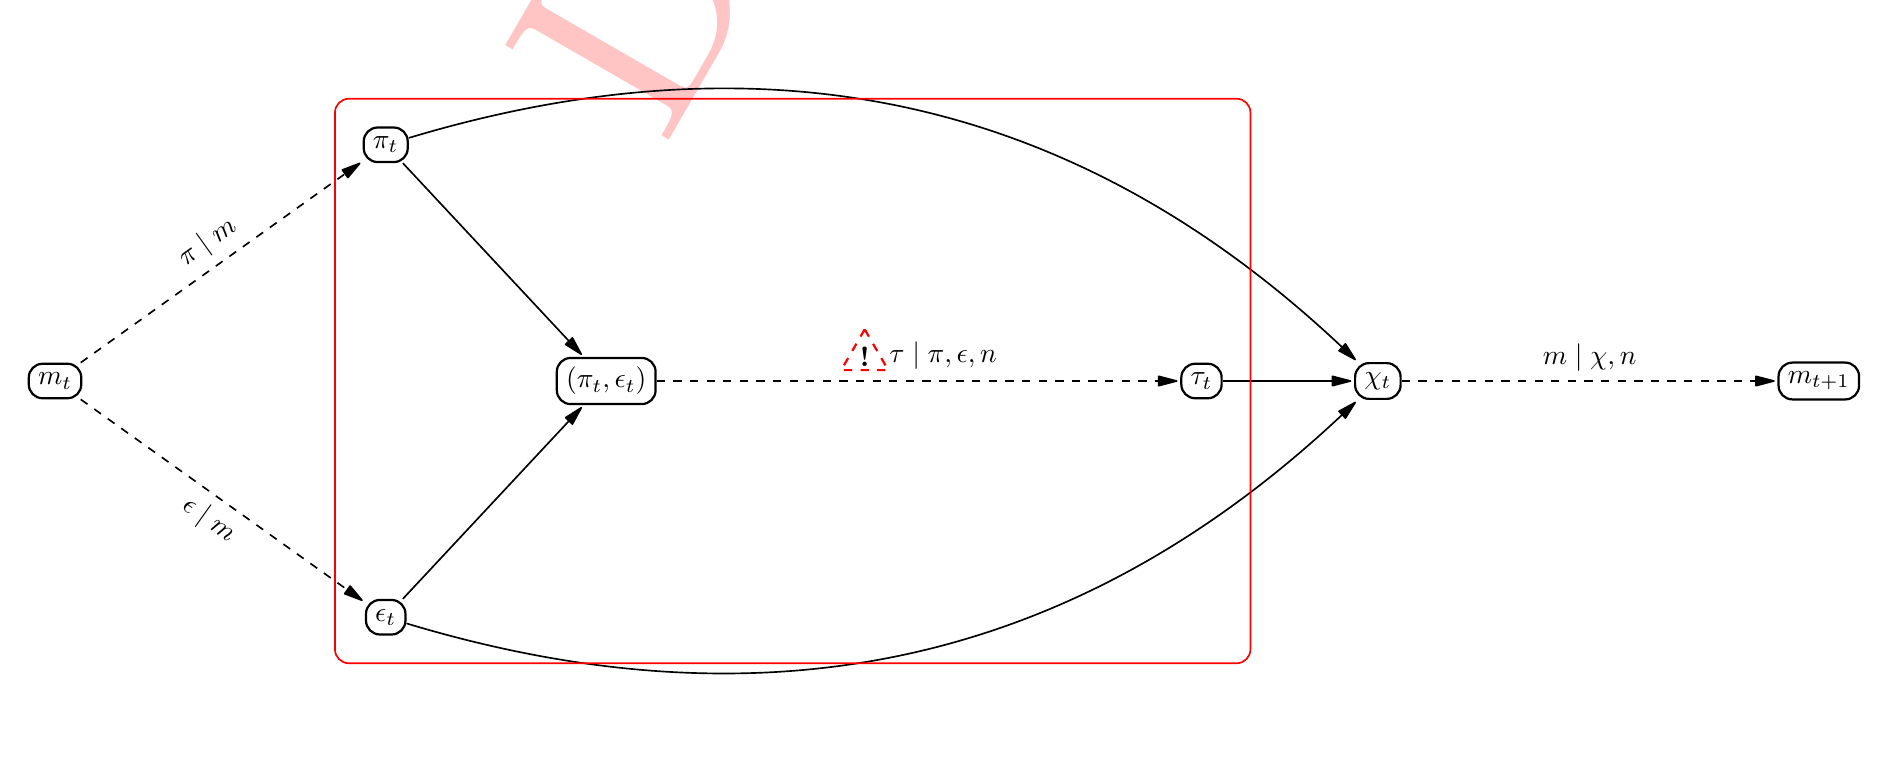
\begin{tikzpicture}[y=-3cm,x=2.8cm,
            > = {Stealth[inset=0pt,length=8pt,angle'=28,round]}, % arrow head style
            shorten > = 1pt, % don't touch arrow head to node
            auto,
%            node distance =1cm and 3cm, % distance between nodes
            semithick, % line style
            box/.style = {draw,red,inner sep=10pt,rounded corners=5pt}
        ]

        \tikzstyle{every state}=[
        rectangle,
        rounded corners=5pt,
            draw = black,
            thick,
            fill = white,
            minimum size = 4mm
        ]


        \node[state] at (0,1) (m) {$\countdetail_t$ };
        \node[state] at (1.5,0) (pi) {$\pi_t$ };
        \node[state] at (1.5,2) (epsilon) {$\epsilon_t$ };
        \node[state] at (2.5,1) (point) {$(\pi_t,\epsilon_t)$};
        \node[state] at (5.2,1) (tau) {$\tau_t$};
        \node[state] at (6,1) (chi) {$\chi_{t}$};
        \node[state] at (8,1) (mm) {$\countdetail_{t+1}$};
        
        \path[->,dashed] (m) edge node[above, sloped]  {$\pi\mid \countdetail$} (pi);
        \path[->,dashed] (m) edge node[below, sloped]  {$\epsilon\mid \countdetail$} (epsilon);
        \path[->] (pi) edge node {} (point);
        \path[->] (epsilon) edge node {} (point);
        \path[->,dashed] (point) edge node[above, sloped]  {\warningsign $\tau\mid \pi, \epsilon,n$} (tau);
        \path[->] (tau) edge node {} (chi);
        \path[->] (pi) edge [bend left] node {} (chi);
        \path[->] (epsilon) edge[bend right] node {} (chi);
        \path[->,dashed] (chi) edge node {$\countdetail\mid \chi,n$} (mm);
        \node[box,fit=(pi) (epsilon) (tau)]{};
    \end{tikzpicture}

\vspace{-1.5cm}}

}
%%%%%%%%%%%%%%%%%%%%%%%%%%%%%%%%%%%%%%%%%%%%%%%%%%%
\def\blockdiagnostic{
\block{Diagnostic}{
\begin{itemize}
\item When distributed according to the posterior law, the $\tau_{v,g,\indexvec{a}}$ are discrete and highly correlated over $g$.
\item Sampling them independently does not work.
\end{itemize}
\vspace{-1cm}

    $$n_{.,s=1,.}=\begin{blockarray}{ccccc}
    &a=A&a=C&a=G&a=T&\\
    \begin{block}{c(cccc)}
 {\scriptscriptstyle v=1}&600&400&0&0\\   
 {\scriptscriptstyle v=2}&400&600&1&0\\
    \end{block}
\end{blockarray} $$

\vspace{-1.6cm}
$$\begin{blockarray}{ccc}
    &&\\&\scriptscriptstyle g=1&\scriptscriptstyle g=2\\
    \begin{block}{c(cc)}
 {\scriptscriptstyle v=1}&A&C\\   
  {\scriptscriptstyle v=2}&A&C\\   
    \end{block}
\end{blockarray} {\overset{ t\to t+1}{\rightarrow}}\begin{blockarray}{ccc}
    &&\\&\scriptscriptstyle g=1&\scriptscriptstyle g=2\\
    \begin{block}{c(cc)}
 {\scriptscriptstyle v=1}&A&C\\   
  {\scriptscriptstyle v=2}&C&C\\   
    \end{block}
\end{blockarray}\overset{t\to t+1}{\rightarrow}\begin{blockarray}{ccc}
    &&\\&\scriptscriptstyle g=1&\scriptscriptstyle g=2\\
    \begin{block}{c(cc)}
 {\scriptscriptstyle v=1}&A&C\\   
  {\scriptscriptstyle v=2}&C&A\\   
    \end{block}
\end{blockarray}$$
}

	 \note[connection, radius=4cm, angle=-85,targetoffsety = -4cm,targetoffsetx = -3.5cm,rotate = 5, innersep=0.1cm, width=11.2cm]{\begin{minipage}{2cm}\sensinterdit\end{minipage}\begin{minipage}{9cm} \begin{Handwriting}



Sampler can't make that jump and stays stuck\end{Handwriting} \end{minipage}}
}
%%%%%%%%%%%%%%%%%%%%%%%%%%%%%%%%%%%%%%%%%%%%%%%%%%%
\def\blockrelax{\innerblock{Relaxation}{
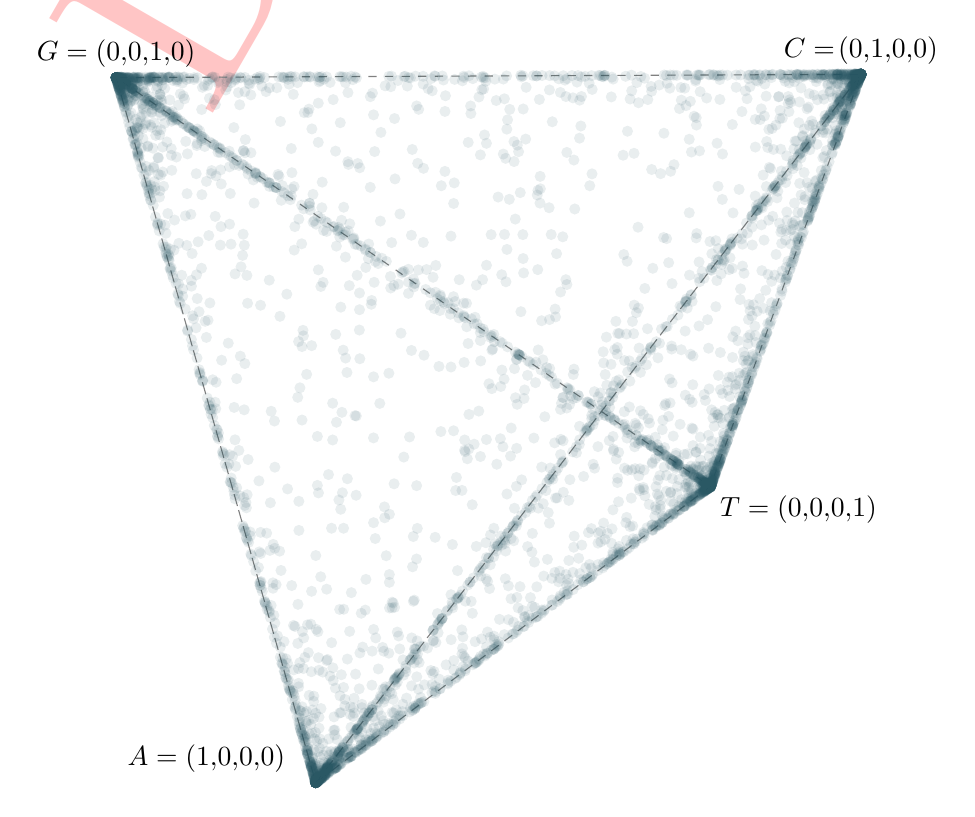
\begin{tikzpicture}[scale=10]


\begin{scope}[rotate around y=45,rotate around z=45]
 
% Draw the vertices of the tetrahedron

\coordinate (A) at (0, 0, 0);
\coordinate (C) at (1, 0, 0);
\coordinate (G) at (0.5, 0.866, 0);
\coordinate (T) at (0.5, 0.2887, 0.816);

%\foreach \p in {A,C,G,T}\fill[black] (\p) circle (0.02);

% Draw the edges of the cube
\draw[white!50!black, dashed]  (A) -- (C) -- (G) -- (A) -- (C) -- (T) -- (A) -- (T) -- (G) --  cycle;



    \pgfmathsetmacro{\alphaa}{0.1}       
       
\fill[color1,  opacity=\alphaa] (0.423,0.586,0.046) circle (.2pt);
         \fill[color1,  opacity=\alphaa] (0.984,0.027,0) circle (.2pt);
         \fill[color1,  opacity=\alphaa] (0.286,0.29,0.207) circle (.2pt);
         \fill[color1,  opacity=\alphaa] (0.842,0.106,0) circle (.2pt);
         \fill[color1,  opacity=\alphaa] (0.604,0.399,0.404) circle (.2pt);
         \fill[color1,  opacity=\alphaa] (0.093,0.02,0.057) circle (.2pt);
         \fill[color1,  opacity=\alphaa] (0,0,0) circle (.2pt);
         \fill[color1,  opacity=\alphaa] (0.231,0,0) circle (.2pt);
         \fill[color1,  opacity=\alphaa] (1,0,0) circle (.2pt);
         \fill[color1,  opacity=\alphaa] (0.36,0.556,0.003) circle (.2pt);
         \fill[color1,  opacity=\alphaa] (0.454,0.593,0.229) circle (.2pt);
         \fill[color1,  opacity=\alphaa] (0.506,0.85,0) circle (.2pt);
         \fill[color1,  opacity=\alphaa] (0.414,0.41,0.052) circle (.2pt);
         \fill[color1,  opacity=\alphaa] (0.533,0.269,0.762) circle (.2pt);
         \fill[color1,  opacity=\alphaa] (0.488,0.837,0) circle (.2pt);
         \fill[color1,  opacity=\alphaa] (0.001,0,0) circle (.2pt);
         \fill[color1,  opacity=\alphaa] (0.364,0.631,0) circle (.2pt);
         \fill[color1,  opacity=\alphaa] (0.495,0.836,0) circle (.2pt);
         \fill[color1,  opacity=\alphaa] (0.996,0.001,0) circle (.2pt);
         \fill[color1,  opacity=\alphaa] (0.999,0,0.001) circle (.2pt);
         \fill[color1,  opacity=\alphaa] (0.453,0.784,0) circle (.2pt);
         \fill[color1,  opacity=\alphaa] (0.405,0.235,0.66) circle (.2pt);
         \fill[color1,  opacity=\alphaa] (0.828,0.099,0.281) circle (.2pt);
         \fill[color1,  opacity=\alphaa] (0.648,0.186,0.526) circle (.2pt);
         \fill[color1,  opacity=\alphaa] (0.488,0.846,0) circle (.2pt);
         \fill[color1,  opacity=\alphaa] (0.47,0.438,0.499) circle (.2pt);
         \fill[color1,  opacity=\alphaa] (0.498,0.863,0) circle (.2pt);
         \fill[color1,  opacity=\alphaa] (0.006,0.01,0) circle (.2pt);
         \fill[color1,  opacity=\alphaa] (0.5,0.839,0.038) circle (.2pt);
         \fill[color1,  opacity=\alphaa] (0.605,0.051,0) circle (.2pt);
         \fill[color1,  opacity=\alphaa] (0.485,0.287,0.782) circle (.2pt);
         \fill[color1,  opacity=\alphaa] (0.516,0.502,0.418) circle (.2pt);
         \fill[color1,  opacity=\alphaa] (0.035,0.025,0.051) circle (.2pt);
         \fill[color1,  opacity=\alphaa] (0.5,0.289,0.816) circle (.2pt);
         \fill[color1,  opacity=\alphaa] (0.267,0.463,0) circle (.2pt);
         \fill[color1,  opacity=\alphaa] (0.5,0.289,0.816) circle (.2pt);
         \fill[color1,  opacity=\alphaa] (0.482,0.827,0) circle (.2pt);
         \fill[color1,  opacity=\alphaa] (0.5,0.298,0.804) circle (.2pt);
         \fill[color1,  opacity=\alphaa] (0.5,0.866,0) circle (.2pt);
         \fill[color1,  opacity=\alphaa] (0.5,0.289,0.816) circle (.2pt);
         \fill[color1,  opacity=\alphaa] (0.844,0.092,0.252) circle (.2pt);
         \fill[color1,  opacity=\alphaa] (0.476,0.583,0.341) circle (.2pt);
         \fill[color1,  opacity=\alphaa] (0.46,0.777,0.029) circle (.2pt);
         \fill[color1,  opacity=\alphaa] (0.996,0.007,0) circle (.2pt);
         \fill[color1,  opacity=\alphaa] (0.392,0.498,0.256) circle (.2pt);
         \fill[color1,  opacity=\alphaa] (0.977,0.013,0.038) circle (.2pt);
         \fill[color1,  opacity=\alphaa] (0.95,0.032,0.077) circle (.2pt);
         \fill[color1,  opacity=\alphaa] (0.436,0.611,0.002) circle (.2pt);
         \fill[color1,  opacity=\alphaa] (0.025,0.029,0.019) circle (.2pt);
         \fill[color1,  opacity=\alphaa] (0.952,0.028,0.079) circle (.2pt);
         \fill[color1,  opacity=\alphaa] (0.975,0.004,0.011) circle (.2pt);
         \fill[color1,  opacity=\alphaa] (0.006,0.002,0.006) circle (.2pt);
         \fill[color1,  opacity=\alphaa] (0.52,0.261,0.738) circle (.2pt);
         \fill[color1,  opacity=\alphaa] (0.319,0.184,0.521) circle (.2pt);
         \fill[color1,  opacity=\alphaa] (0.382,0.238,0.595) circle (.2pt);
         \fill[color1,  opacity=\alphaa] (0.207,0.357,0) circle (.2pt);
         \fill[color1,  opacity=\alphaa] (0.5,0.851,0.022) circle (.2pt);
         \fill[color1,  opacity=\alphaa] (0.575,0.22,0.616) circle (.2pt);
         \fill[color1,  opacity=\alphaa] (0.489,0.804,0.06) circle (.2pt);
         \fill[color1,  opacity=\alphaa] (0.968,0.006,0) circle (.2pt);
         \fill[color1,  opacity=\alphaa] (0.403,0,0) circle (.2pt);
         \fill[color1,  opacity=\alphaa] (0.008,0,0) circle (.2pt);
         \fill[color1,  opacity=\alphaa] (0.523,0.275,0.778) circle (.2pt);
         \fill[color1,  opacity=\alphaa] (0.5,0.474,0.554) circle (.2pt);
         \fill[color1,  opacity=\alphaa] (0.516,0.822,0.022) circle (.2pt);
         \fill[color1,  opacity=\alphaa] (0.021,0.001,0.003) circle (.2pt);
         \fill[color1,  opacity=\alphaa] (0.5,0.866,0) circle (.2pt);
         \fill[color1,  opacity=\alphaa] (0.339,0,0) circle (.2pt);
         \fill[color1,  opacity=\alphaa] (0.505,0.856,0.002) circle (.2pt);
         \fill[color1,  opacity=\alphaa] (0.002,0,0) circle (.2pt);
         \fill[color1,  opacity=\alphaa] (0.132,0.044,0.125) circle (.2pt);
         \fill[color1,  opacity=\alphaa] (0.508,0.851,0) circle (.2pt);
         \fill[color1,  opacity=\alphaa] (0,0,0) circle (.2pt);
         \fill[color1,  opacity=\alphaa] (0.831,0.29,0.003) circle (.2pt);
         \fill[color1,  opacity=\alphaa] (0,0,0) circle (.2pt);
         \fill[color1,  opacity=\alphaa] (0.502,0.301,0.793) circle (.2pt);
         \fill[color1,  opacity=\alphaa] (0.598,0.67,0.001) circle (.2pt);
         \fill[color1,  opacity=\alphaa] (0.5,0.846,0.028) circle (.2pt);
         \fill[color1,  opacity=\alphaa] (0.979,0.037,0) circle (.2pt);
         \fill[color1,  opacity=\alphaa] (0.548,0.78,0) circle (.2pt);
         \fill[color1,  opacity=\alphaa] (0.528,0.273,0.771) circle (.2pt);
         \fill[color1,  opacity=\alphaa] (0.445,0.769,0) circle (.2pt);
         \fill[color1,  opacity=\alphaa] (1,0,0) circle (.2pt);
         \fill[color1,  opacity=\alphaa] (0.461,0.264,0.748) circle (.2pt);
         \fill[color1,  opacity=\alphaa] (0.486,0.779,0.087) circle (.2pt);
         \fill[color1,  opacity=\alphaa] (0.074,0.018,0.034) circle (.2pt);
         \fill[color1,  opacity=\alphaa] (0.205,0.014,0.04) circle (.2pt);
         \fill[color1,  opacity=\alphaa] (0.501,0.288,0.815) circle (.2pt);
         \fill[color1,  opacity=\alphaa] (0.901,0.171,0) circle (.2pt);
         \fill[color1,  opacity=\alphaa] (0.5,0.305,0.793) circle (.2pt);
         \fill[color1,  opacity=\alphaa] (0.476,0.275,0.777) circle (.2pt);
         \fill[color1,  opacity=\alphaa] (0.563,0.749,0.011) circle (.2pt);
         \fill[color1,  opacity=\alphaa] (0.194,0.005,0.014) circle (.2pt);
         \fill[color1,  opacity=\alphaa] (0.5,0.289,0.816) circle (.2pt);
         \fill[color1,  opacity=\alphaa] (0.984,0,0) circle (.2pt);
         \fill[color1,  opacity=\alphaa] (0.97,0.016,0.013) circle (.2pt);
         \fill[color1,  opacity=\alphaa] (0.494,0.855,0) circle (.2pt);
         \fill[color1,  opacity=\alphaa] (0.497,0.287,0.811) circle (.2pt);
         \fill[color1,  opacity=\alphaa] (0.883,0.202,0) circle (.2pt);
         \fill[color1,  opacity=\alphaa] (0.305,0.055,0.001) circle (.2pt);
         \fill[color1,  opacity=\alphaa] (0.356,0.211,0.574) circle (.2pt);
         \fill[color1,  opacity=\alphaa] (0.02,0.035,0) circle (.2pt);
         \fill[color1,  opacity=\alphaa] (0.796,0.117,0.33) circle (.2pt);
         \fill[color1,  opacity=\alphaa] (0.391,0.161,0.43) circle (.2pt);
         \fill[color1,  opacity=\alphaa] (0.099,0.001,0) circle (.2pt);
         \fill[color1,  opacity=\alphaa] (0,0,0) circle (.2pt);
         \fill[color1,  opacity=\alphaa] (0.483,0.411,0.603) circle (.2pt);
         \fill[color1,  opacity=\alphaa] (0.5,0.289,0.816) circle (.2pt);
         \fill[color1,  opacity=\alphaa] (0.499,0.288,0.815) circle (.2pt);
         \fill[color1,  opacity=\alphaa] (0.499,0.864,0) circle (.2pt);
         \fill[color1,  opacity=\alphaa] (0.496,0.285,0.807) circle (.2pt);
         \fill[color1,  opacity=\alphaa] (0.493,0.852,0.002) circle (.2pt);
         \fill[color1,  opacity=\alphaa] (0.501,0.296,0.803) circle (.2pt);
         \fill[color1,  opacity=\alphaa] (0.155,0.26,0) circle (.2pt);
         \fill[color1,  opacity=\alphaa] (0.493,0.285,0.806) circle (.2pt);
         \fill[color1,  opacity=\alphaa] (0.581,0.14,0.377) circle (.2pt);
         \fill[color1,  opacity=\alphaa] (0.738,0,0) circle (.2pt);
         \fill[color1,  opacity=\alphaa] (0.655,0.199,0.563) circle (.2pt);
         \fill[color1,  opacity=\alphaa] (0.492,0.694,0.221) circle (.2pt);
         \fill[color1,  opacity=\alphaa] (0.502,0.86,0.004) circle (.2pt);
         \fill[color1,  opacity=\alphaa] (0.725,0.023,0.066) circle (.2pt);
         \fill[color1,  opacity=\alphaa] (0.029,0.049,0) circle (.2pt);
         \fill[color1,  opacity=\alphaa] (0.262,0,0) circle (.2pt);
         \fill[color1,  opacity=\alphaa] (0.382,0.368,0.414) circle (.2pt);
         \fill[color1,  opacity=\alphaa] (0.999,0.001,0.002) circle (.2pt);
         \fill[color1,  opacity=\alphaa] (0.5,0.313,0.783) circle (.2pt);
         \fill[color1,  opacity=\alphaa] (0.999,0,0) circle (.2pt);
         \fill[color1,  opacity=\alphaa] (0.496,0.858,0.001) circle (.2pt);
         \fill[color1,  opacity=\alphaa] (0.71,0.171,0.469) circle (.2pt);
         \fill[color1,  opacity=\alphaa] (0.025,0.014,0.041) circle (.2pt);
         \fill[color1,  opacity=\alphaa] (0.049,0,0) circle (.2pt);
         \fill[color1,  opacity=\alphaa] (0.439,0.15,0.424) circle (.2pt);
         \fill[color1,  opacity=\alphaa] (0.261,0.151,0.418) circle (.2pt);
         \fill[color1,  opacity=\alphaa] (0,0,0) circle (.2pt);
         \fill[color1,  opacity=\alphaa] (0.5,0.864,0.002) circle (.2pt);
         \fill[color1,  opacity=\alphaa] (0.347,0.427,0.242) circle (.2pt);
         \fill[color1,  opacity=\alphaa] (0.95,0.029,0.081) circle (.2pt);
         \fill[color1,  opacity=\alphaa] (1,0,0) circle (.2pt);
         \fill[color1,  opacity=\alphaa] (0.988,0.02,0) circle (.2pt);
         \fill[color1,  opacity=\alphaa] (0.784,0.124,0.35) circle (.2pt);
         \fill[color1,  opacity=\alphaa] (0.468,0.274,0.759) circle (.2pt);
         \fill[color1,  opacity=\alphaa] (0.286,0.093,0.263) circle (.2pt);
         \fill[color1,  opacity=\alphaa] (0.493,0.847,0.009) circle (.2pt);
         \fill[color1,  opacity=\alphaa] (0.927,0,0) circle (.2pt);
         \fill[color1,  opacity=\alphaa] (0.429,0,0) circle (.2pt);
         \fill[color1,  opacity=\alphaa] (0.916,0.047,0.133) circle (.2pt);
         \fill[color1,  opacity=\alphaa] (0.613,0,0.001) circle (.2pt);
         \fill[color1,  opacity=\alphaa] (0.5,0.327,0.763) circle (.2pt);
         \fill[color1,  opacity=\alphaa] (0.963,0.007,0) circle (.2pt);
         \fill[color1,  opacity=\alphaa] (0.534,0.268,0.759) circle (.2pt);
         \fill[color1,  opacity=\alphaa] (0.483,0.309,0.747) circle (.2pt);
         \fill[color1,  opacity=\alphaa] (0.499,0.865,0) circle (.2pt);
         \fill[color1,  opacity=\alphaa] (0.285,0.452,0.057) circle (.2pt);
         \fill[color1,  opacity=\alphaa] (0.848,0.088,0.247) circle (.2pt);
         \fill[color1,  opacity=\alphaa] (0.118,0.203,0.003) circle (.2pt);
         \fill[color1,  opacity=\alphaa] (1,0,0) circle (.2pt);
         \fill[color1,  opacity=\alphaa] (0.261,0.018,0.05) circle (.2pt);
         \fill[color1,  opacity=\alphaa] (0.5,0.866,0) circle (.2pt);
         \fill[color1,  opacity=\alphaa] (0.5,0.339,0.744) circle (.2pt);
         \fill[color1,  opacity=\alphaa] (0.066,0.113,0) circle (.2pt);
         \fill[color1,  opacity=\alphaa] (0.507,0.285,0.806) circle (.2pt);
         \fill[color1,  opacity=\alphaa] (0.023,0.004,0.01) circle (.2pt);
         \fill[color1,  opacity=\alphaa] (0.139,0.148,0) circle (.2pt);
         \fill[color1,  opacity=\alphaa] (0.507,0.332,0.74) circle (.2pt);
         \fill[color1,  opacity=\alphaa] (0.5,0.865,0.001) circle (.2pt);
         \fill[color1,  opacity=\alphaa] (0.5,0.301,0.799) circle (.2pt);
         \fill[color1,  opacity=\alphaa] (0.012,0.021,0) circle (.2pt);
         \fill[color1,  opacity=\alphaa] (0.459,0.767,0) circle (.2pt);
         \fill[color1,  opacity=\alphaa] (0.779,0.128,0.36) circle (.2pt);
         \fill[color1,  opacity=\alphaa] (0.5,0.699,0.236) circle (.2pt);
         \fill[color1,  opacity=\alphaa] (0.868,0.229,0) circle (.2pt);
         \fill[color1,  opacity=\alphaa] (0.004,0,0) circle (.2pt);
         \fill[color1,  opacity=\alphaa] (0.5,0.663,0.288) circle (.2pt);
         \fill[color1,  opacity=\alphaa] (0.496,0.507,0.498) circle (.2pt);
         \fill[color1,  opacity=\alphaa] (0.184,0.289,0.043) circle (.2pt);
         \fill[color1,  opacity=\alphaa] (0.5,0.863,0.004) circle (.2pt);
         \fill[color1,  opacity=\alphaa] (0.955,0.032,0.066) circle (.2pt);
         \fill[color1,  opacity=\alphaa] (0.484,0.838,0.002) circle (.2pt);
         \fill[color1,  opacity=\alphaa] (0.043,0.074,0) circle (.2pt);
         \fill[color1,  opacity=\alphaa] (0.501,0.31,0.784) circle (.2pt);
         \fill[color1,  opacity=\alphaa] (0.992,0.009,0) circle (.2pt);
         \fill[color1,  opacity=\alphaa] (0.491,0.851,0) circle (.2pt);
         \fill[color1,  opacity=\alphaa] (0.499,0.291,0.809) circle (.2pt);
         \fill[color1,  opacity=\alphaa] (0,0,0) circle (.2pt);
         \fill[color1,  opacity=\alphaa] (0.047,0.012,0.033) circle (.2pt);
         \fill[color1,  opacity=\alphaa] (0.961,0.067,0) circle (.2pt);
         \fill[color1,  opacity=\alphaa] (0.502,0.287,0.813) circle (.2pt);
         \fill[color1,  opacity=\alphaa] (0.499,0.288,0.814) circle (.2pt);
         \fill[color1,  opacity=\alphaa] (0.181,0.161,0) circle (.2pt);
         \fill[color1,  opacity=\alphaa] (0.455,0.783,0.001) circle (.2pt);
         \fill[color1,  opacity=\alphaa] (0.875,0,0) circle (.2pt);
         \fill[color1,  opacity=\alphaa] (0.505,0.304,0.782) circle (.2pt);
         \fill[color1,  opacity=\alphaa] (0.66,0.221,0.519) circle (.2pt);
         \fill[color1,  opacity=\alphaa] (0.564,0.252,0.712) circle (.2pt);
         \fill[color1,  opacity=\alphaa] (0.5,0.289,0.816) circle (.2pt);
         \fill[color1,  opacity=\alphaa] (0.5,0.289,0.816) circle (.2pt);
         \fill[color1,  opacity=\alphaa] (0.667,0.325,0.355) circle (.2pt);
         \fill[color1,  opacity=\alphaa] (1,0,0) circle (.2pt);
         \fill[color1,  opacity=\alphaa] (0.406,0.454,0.29) circle (.2pt);
         \fill[color1,  opacity=\alphaa] (0.55,0.776,0.004) circle (.2pt);
         \fill[color1,  opacity=\alphaa] (0.309,0.179,0.505) circle (.2pt);
         \fill[color1,  opacity=\alphaa] (0.5,0.861,0.007) circle (.2pt);
         \fill[color1,  opacity=\alphaa] (0.47,0.723,0.127) circle (.2pt);
         \fill[color1,  opacity=\alphaa] (0.061,0.03,0.083) circle (.2pt);
         \fill[color1,  opacity=\alphaa] (1,0,0) circle (.2pt);
         \fill[color1,  opacity=\alphaa] (0.5,0.288,0.816) circle (.2pt);
         \fill[color1,  opacity=\alphaa] (0.001,0,0) circle (.2pt);
         \fill[color1,  opacity=\alphaa] (0.5,0.865,0) circle (.2pt);
         \fill[color1,  opacity=\alphaa] (0.883,0.203,0) circle (.2pt);
         \fill[color1,  opacity=\alphaa] (0.224,0,0) circle (.2pt);
         \fill[color1,  opacity=\alphaa] (0.849,0.234,0) circle (.2pt);
         \fill[color1,  opacity=\alphaa] (0.484,0,0) circle (.2pt);
         \fill[color1,  opacity=\alphaa] (0.732,0.154,0.437) circle (.2pt);
         \fill[color1,  opacity=\alphaa] (0.998,0.001,0.004) circle (.2pt);
         \fill[color1,  opacity=\alphaa] (0.46,0.424,0.526) circle (.2pt);
         \fill[color1,  opacity=\alphaa] (0.524,0.825,0) circle (.2pt);
         \fill[color1,  opacity=\alphaa] (0.531,0.026,0.054) circle (.2pt);
         \fill[color1,  opacity=\alphaa] (0.022,0.001,0) circle (.2pt);
         \fill[color1,  opacity=\alphaa] (0.733,0.037,0.099) circle (.2pt);
         \fill[color1,  opacity=\alphaa] (0.5,0.339,0.745) circle (.2pt);
         \fill[color1,  opacity=\alphaa] (0.993,0.013,0) circle (.2pt);
         \fill[color1,  opacity=\alphaa] (0.5,0.857,0.013) circle (.2pt);
         \fill[color1,  opacity=\alphaa] (0.995,0.001,0.001) circle (.2pt);
         \fill[color1,  opacity=\alphaa] (0.075,0.103,0.039) circle (.2pt);
         \fill[color1,  opacity=\alphaa] (0.994,0.003,0.009) circle (.2pt);
         \fill[color1,  opacity=\alphaa] (0.855,0.021,0) circle (.2pt);
         \fill[color1,  opacity=\alphaa] (0.5,0.856,0.014) circle (.2pt);
         \fill[color1,  opacity=\alphaa] (0.995,0.003,0.008) circle (.2pt);
         \fill[color1,  opacity=\alphaa] (1,0,0) circle (.2pt);
         \fill[color1,  opacity=\alphaa] (0.002,0.001,0) circle (.2pt);
         \fill[color1,  opacity=\alphaa] (0.994,0,0.001) circle (.2pt);
         \fill[color1,  opacity=\alphaa] (0.493,0.281,0.794) circle (.2pt);
         \fill[color1,  opacity=\alphaa] (0.825,0.303,0) circle (.2pt);
         \fill[color1,  opacity=\alphaa] (0.501,0.859,0.008) circle (.2pt);
         \fill[color1,  opacity=\alphaa] (0.496,0.286,0.808) circle (.2pt);
         \fill[color1,  opacity=\alphaa] (0.497,0.283,0.799) circle (.2pt);
         \fill[color1,  opacity=\alphaa] (0.501,0.288,0.814) circle (.2pt);
         \fill[color1,  opacity=\alphaa] (0.502,0.298,0.798) circle (.2pt);
         \fill[color1,  opacity=\alphaa] (0.229,0.059,0.017) circle (.2pt);
         \fill[color1,  opacity=\alphaa] (0.5,0.858,0.011) circle (.2pt);
         \fill[color1,  opacity=\alphaa] (0.5,0.866,0) circle (.2pt);
         \fill[color1,  opacity=\alphaa] (0.17,0.06,0) circle (.2pt);
         \fill[color1,  opacity=\alphaa] (0.398,0.686,0.006) circle (.2pt);
         \fill[color1,  opacity=\alphaa] (0.949,0.071,0) circle (.2pt);
         \fill[color1,  opacity=\alphaa] (0.5,0.289,0.816) circle (.2pt);
         \fill[color1,  opacity=\alphaa] (0.976,0.03,0) circle (.2pt);
         \fill[color1,  opacity=\alphaa] (0.286,0.109,0.003) circle (.2pt);
         \fill[color1,  opacity=\alphaa] (0.002,0.001,0.002) circle (.2pt);
         \fill[color1,  opacity=\alphaa] (0.345,0.559,0) circle (.2pt);
         \fill[color1,  opacity=\alphaa] (0.456,0.633,0.219) circle (.2pt);
         \fill[color1,  opacity=\alphaa] (0.499,0.833,0.045) circle (.2pt);
         \fill[color1,  opacity=\alphaa] (0.01,0.005,0.002) circle (.2pt);
         \fill[color1,  opacity=\alphaa] (0.491,0.33,0.735) circle (.2pt);
         \fill[color1,  opacity=\alphaa] (0.554,0.752,0) circle (.2pt);
         \fill[color1,  opacity=\alphaa] (0.493,0.854,0) circle (.2pt);
         \fill[color1,  opacity=\alphaa] (0.999,0.001,0) circle (.2pt);
         \fill[color1,  opacity=\alphaa] (0.984,0.028,0) circle (.2pt);
         \fill[color1,  opacity=\alphaa] (0.999,0,0) circle (.2pt);
         \fill[color1,  opacity=\alphaa] (0.071,0.041,0.117) circle (.2pt);
         \fill[color1,  opacity=\alphaa] (0,0,0) circle (.2pt);
         \fill[color1,  opacity=\alphaa] (0.572,0.649,0.13) circle (.2pt);
         \fill[color1,  opacity=\alphaa] (0.406,0.235,0.662) circle (.2pt);
         \fill[color1,  opacity=\alphaa] (0.001,0.001,0.001) circle (.2pt);
         \fill[color1,  opacity=\alphaa] (0.998,0.001,0.003) circle (.2pt);
         \fill[color1,  opacity=\alphaa] (0.334,0,0) circle (.2pt);
         \fill[color1,  opacity=\alphaa] (0.989,0,0) circle (.2pt);
         \fill[color1,  opacity=\alphaa] (0.716,0.485,0.005) circle (.2pt);
         \fill[color1,  opacity=\alphaa] (0.002,0.004,0) circle (.2pt);
         \fill[color1,  opacity=\alphaa] (0.948,0.033,0.08) circle (.2pt);
         \fill[color1,  opacity=\alphaa] (0.996,0.002,0.007) circle (.2pt);
         \fill[color1,  opacity=\alphaa] (0.03,0.048,0) circle (.2pt);
         \fill[color1,  opacity=\alphaa] (0.503,0.335,0.744) circle (.2pt);
         \fill[color1,  opacity=\alphaa] (0.241,0.001,0) circle (.2pt);
         \fill[color1,  opacity=\alphaa] (0.063,0,0) circle (.2pt);
         \fill[color1,  opacity=\alphaa] (0.5,0.289,0.816) circle (.2pt);
         \fill[color1,  opacity=\alphaa] (0,0,0) circle (.2pt);
         \fill[color1,  opacity=\alphaa] (0.026,0,0) circle (.2pt);
         \fill[color1,  opacity=\alphaa] (0.021,0.037,0) circle (.2pt);
         \fill[color1,  opacity=\alphaa] (0.511,0.836,0.013) circle (.2pt);
         \fill[color1,  opacity=\alphaa] (0.953,0.027,0.076) circle (.2pt);
         \fill[color1,  opacity=\alphaa] (0.013,0,0) circle (.2pt);
         \fill[color1,  opacity=\alphaa] (0.452,0.288,0.7) circle (.2pt);
         \fill[color1,  opacity=\alphaa] (0.004,0.002,0.006) circle (.2pt);
         \fill[color1,  opacity=\alphaa] (0.455,0.055,0) circle (.2pt);
         \fill[color1,  opacity=\alphaa] (0.775,0.13,0.367) circle (.2pt);
         \fill[color1,  opacity=\alphaa] (0.5,0.289,0.816) circle (.2pt);
         \fill[color1,  opacity=\alphaa] (0.841,0,0) circle (.2pt);
         \fill[color1,  opacity=\alphaa] (0.732,0.004,0.009) circle (.2pt);
         \fill[color1,  opacity=\alphaa] (0.488,0.282,0.797) circle (.2pt);
         \fill[color1,  opacity=\alphaa] (0.003,0.005,0) circle (.2pt);
         \fill[color1,  opacity=\alphaa] (0.5,0.866,0.001) circle (.2pt);
         \fill[color1,  opacity=\alphaa] (0.513,0.281,0.796) circle (.2pt);
         \fill[color1,  opacity=\alphaa] (0.497,0.31,0.778) circle (.2pt);
         \fill[color1,  opacity=\alphaa] (0.83,0.289,0.007) circle (.2pt);
         \fill[color1,  opacity=\alphaa] (0.501,0.288,0.814) circle (.2pt);
         \fill[color1,  opacity=\alphaa] (0.5,0.29,0.815) circle (.2pt);
         \fill[color1,  opacity=\alphaa] (0.971,0.02,0.041) circle (.2pt);
         \fill[color1,  opacity=\alphaa] (0,0,0) circle (.2pt);
         \fill[color1,  opacity=\alphaa] (0.513,0.82,0.034) circle (.2pt);
         \fill[color1,  opacity=\alphaa] (0.518,0.67,0.234) circle (.2pt);
         \fill[color1,  opacity=\alphaa] (0.989,0.006,0.018) circle (.2pt);
         \fill[color1,  opacity=\alphaa] (1,0,0) circle (.2pt);
         \fill[color1,  opacity=\alphaa] (0.5,0.854,0.017) circle (.2pt);
         \fill[color1,  opacity=\alphaa] (0.501,0.797,0.059) circle (.2pt);
         \fill[color1,  opacity=\alphaa] (0.783,0.139,0.335) circle (.2pt);
         \fill[color1,  opacity=\alphaa] (0.194,0.135,0.01) circle (.2pt);
         \fill[color1,  opacity=\alphaa] (0.504,0.86,0) circle (.2pt);
         \fill[color1,  opacity=\alphaa] (0.915,0.049,0.139) circle (.2pt);
         \fill[color1,  opacity=\alphaa] (0.006,0.003,0.01) circle (.2pt);
         \fill[color1,  opacity=\alphaa] (0.5,0.393,0.669) circle (.2pt);
         \fill[color1,  opacity=\alphaa] (0.001,0,0.001) circle (.2pt);
         \fill[color1,  opacity=\alphaa] (0.916,0.089,0.065) circle (.2pt);
         \fill[color1,  opacity=\alphaa] (0.003,0,0) circle (.2pt);
         \fill[color1,  opacity=\alphaa] (0.552,0.216,0.612) circle (.2pt);
         \fill[color1,  opacity=\alphaa] (0.987,0.023,0) circle (.2pt);
         \fill[color1,  opacity=\alphaa] (0.883,0,0) circle (.2pt);
         \fill[color1,  opacity=\alphaa] (0.362,0,0) circle (.2pt);
         \fill[color1,  opacity=\alphaa] (0.952,0.003,0.003) circle (.2pt);
         \fill[color1,  opacity=\alphaa] (0.091,0.151,0.009) circle (.2pt);
         \fill[color1,  opacity=\alphaa] (0.426,0.733,0.007) circle (.2pt);
         \fill[color1,  opacity=\alphaa] (0.5,0.861,0.007) circle (.2pt);
         \fill[color1,  opacity=\alphaa] (0.5,0.289,0.816) circle (.2pt);
         \fill[color1,  opacity=\alphaa] (0.62,0.658,0) circle (.2pt);
         \fill[color1,  opacity=\alphaa] (0.785,0.341,0.044) circle (.2pt);
         \fill[color1,  opacity=\alphaa] (0.004,0.007,0) circle (.2pt);
         \fill[color1,  opacity=\alphaa] (0.702,0.185,0.416) circle (.2pt);
         \fill[color1,  opacity=\alphaa] (0.071,0.041,0.116) circle (.2pt);
         \fill[color1,  opacity=\alphaa] (0.498,0.311,0.781) circle (.2pt);
         \fill[color1,  opacity=\alphaa] (0.499,0.86,0.006) circle (.2pt);
         \fill[color1,  opacity=\alphaa] (0.508,0.85,0) circle (.2pt);
         \fill[color1,  opacity=\alphaa] (0.006,0,0) circle (.2pt);
         \fill[color1,  opacity=\alphaa] (0.523,0.826,0) circle (.2pt);
         \fill[color1,  opacity=\alphaa] (0.001,0,0) circle (.2pt);
         \fill[color1,  opacity=\alphaa] (0.49,0.087,0.243) circle (.2pt);
         \fill[color1,  opacity=\alphaa] (0.5,0.857,0.013) circle (.2pt);
         \fill[color1,  opacity=\alphaa] (0.5,0.771,0.134) circle (.2pt);
         \fill[color1,  opacity=\alphaa] (0.444,0.365,0.572) circle (.2pt);
         \fill[color1,  opacity=\alphaa] (0.313,0.175,0.494) circle (.2pt);
         \fill[color1,  opacity=\alphaa] (0.497,0.287,0.812) circle (.2pt);
         \fill[color1,  opacity=\alphaa] (0.167,0.096,0.273) circle (.2pt);
         \fill[color1,  opacity=\alphaa] (0.5,0.528,0.477) circle (.2pt);
         \fill[color1,  opacity=\alphaa] (0.473,0.791,0.039) circle (.2pt);
         \fill[color1,  opacity=\alphaa] (0.892,0.187,0) circle (.2pt);
         \fill[color1,  opacity=\alphaa] (0.187,0.003,0) circle (.2pt);
         \fill[color1,  opacity=\alphaa] (0.497,0.857,0) circle (.2pt);
         \fill[color1,  opacity=\alphaa] (1,0,0) circle (.2pt);
         \fill[color1,  opacity=\alphaa] (0.031,0.018,0.051) circle (.2pt);
         \fill[color1,  opacity=\alphaa] (0.495,0.857,0) circle (.2pt);
         \fill[color1,  opacity=\alphaa] (0.807,0.3,0) circle (.2pt);
         \fill[color1,  opacity=\alphaa] (0.226,0.131,0.37) circle (.2pt);
         \fill[color1,  opacity=\alphaa] (0.984,0,0) circle (.2pt);
         \fill[color1,  opacity=\alphaa] (0.498,0.288,0.813) circle (.2pt);
         \fill[color1,  opacity=\alphaa] (0.011,0.019,0) circle (.2pt);
         \fill[color1,  opacity=\alphaa] (0.5,0.289,0.816) circle (.2pt);
         \fill[color1,  opacity=\alphaa] (0.936,0.11,0) circle (.2pt);
         \fill[color1,  opacity=\alphaa] (0.491,0.283,0.801) circle (.2pt);
         \fill[color1,  opacity=\alphaa] (0.419,0.242,0.675) circle (.2pt);
         \fill[color1,  opacity=\alphaa] (0.538,0.267,0.754) circle (.2pt);
         \fill[color1,  opacity=\alphaa] (0.501,0.288,0.814) circle (.2pt);
         \fill[color1,  opacity=\alphaa] (0.5,0.355,0.722) circle (.2pt);
         \fill[color1,  opacity=\alphaa] (0,0.001,0) circle (.2pt);
         \fill[color1,  opacity=\alphaa] (0.286,0.165,0.467) circle (.2pt);
         \fill[color1,  opacity=\alphaa] (0.5,0.67,0.277) circle (.2pt);
         \fill[color1,  opacity=\alphaa] (0.03,0,0) circle (.2pt);
         \fill[color1,  opacity=\alphaa] (0.072,0.035,0.099) circle (.2pt);
         \fill[color1,  opacity=\alphaa] (0.491,0.283,0.8) circle (.2pt);
         \fill[color1,  opacity=\alphaa] (0.113,0.146,0) circle (.2pt);
         \fill[color1,  opacity=\alphaa] (0.5,0.445,0.594) circle (.2pt);
         \fill[color1,  opacity=\alphaa] (0.246,0.426,0) circle (.2pt);
         \fill[color1,  opacity=\alphaa] (0.528,0.219,0.618) circle (.2pt);
         \fill[color1,  opacity=\alphaa] (0.985,0.012,0.021) circle (.2pt);
         \fill[color1,  opacity=\alphaa] (0.503,0.291,0.803) circle (.2pt);
         \fill[color1,  opacity=\alphaa] (0.5,0.85,0.023) circle (.2pt);
         \fill[color1,  opacity=\alphaa] (0.201,0.339,0.012) circle (.2pt);
         \fill[color1,  opacity=\alphaa] (0.5,0.766,0.141) circle (.2pt);
         \fill[color1,  opacity=\alphaa] (0.069,0.075,0.063) circle (.2pt);
         \fill[color1,  opacity=\alphaa] (0.999,0,0.001) circle (.2pt);
         \fill[color1,  opacity=\alphaa] (0.722,0.161,0.454) circle (.2pt);
         \fill[color1,  opacity=\alphaa] (0.501,0.3,0.798) circle (.2pt);
         \fill[color1,  opacity=\alphaa] (0.264,0.153,0.432) circle (.2pt);
         \fill[color1,  opacity=\alphaa] (0.077,0,0) circle (.2pt);
         \fill[color1,  opacity=\alphaa] (0.812,0.088,0.239) circle (.2pt);
         \fill[color1,  opacity=\alphaa] (0.565,0.488,0.376) circle (.2pt);
         \fill[color1,  opacity=\alphaa] (0.968,0.055,0) circle (.2pt);
         \fill[color1,  opacity=\alphaa] (0,0,0.001) circle (.2pt);
         \fill[color1,  opacity=\alphaa] (0.526,0.822,0) circle (.2pt);
         \fill[color1,  opacity=\alphaa] (0.467,0.27,0.762) circle (.2pt);
         \fill[color1,  opacity=\alphaa] (0.025,0,0) circle (.2pt);
         \fill[color1,  opacity=\alphaa] (0.5,0.325,0.765) circle (.2pt);
         \fill[color1,  opacity=\alphaa] (0.257,0.301,0.143) circle (.2pt);
         \fill[color1,  opacity=\alphaa] (0.009,0,0.001) circle (.2pt);
         \fill[color1,  opacity=\alphaa] (0.686,0.53,0.019) circle (.2pt);
         \fill[color1,  opacity=\alphaa] (0.5,0.866,0) circle (.2pt);
         \fill[color1,  opacity=\alphaa] (0.735,0.191,0.38) circle (.2pt);
         \fill[color1,  opacity=\alphaa] (0.499,0.864,0) circle (.2pt);
         \fill[color1,  opacity=\alphaa] (0,0,0) circle (.2pt);
         \fill[color1,  opacity=\alphaa] (0.971,0.051,0) circle (.2pt);
         \fill[color1,  opacity=\alphaa] (0.934,0.047,0) circle (.2pt);
         \fill[color1,  opacity=\alphaa] (0.5,0.501,0.517) circle (.2pt);
         \fill[color1,  opacity=\alphaa] (0.125,0.189,0.037) circle (.2pt);
         \fill[color1,  opacity=\alphaa] (0.5,0.861,0.006) circle (.2pt);
         \fill[color1,  opacity=\alphaa] (0.5,0.788,0.109) circle (.2pt);
         \fill[color1,  opacity=\alphaa] (0.003,0.003,0.002) circle (.2pt);
         \fill[color1,  opacity=\alphaa] (0.501,0.865,0) circle (.2pt);
         \fill[color1,  opacity=\alphaa] (0.931,0.072,0.012) circle (.2pt);
         \fill[color1,  opacity=\alphaa] (0.5,0.865,0) circle (.2pt);
         \fill[color1,  opacity=\alphaa] (1,0.001,0) circle (.2pt);
         \fill[color1,  opacity=\alphaa] (0.004,0.007,0) circle (.2pt);
         \fill[color1,  opacity=\alphaa] (0.237,0.395,0) circle (.2pt);
         \fill[color1,  opacity=\alphaa] (0.499,0.294,0.807) circle (.2pt);
         \fill[color1,  opacity=\alphaa] (0.516,0.28,0.791) circle (.2pt);
         \fill[color1,  opacity=\alphaa] (0.461,0.172,0.486) circle (.2pt);
         \fill[color1,  opacity=\alphaa] (0.454,0.262,0.741) circle (.2pt);
         \fill[color1,  opacity=\alphaa] (0.013,0,0) circle (.2pt);
         \fill[color1,  opacity=\alphaa] (0.409,0.238,0.665) circle (.2pt);
         \fill[color1,  opacity=\alphaa] (0.5,0.866,0) circle (.2pt);
         \fill[color1,  opacity=\alphaa] (0.485,0.363,0.674) circle (.2pt);
         \fill[color1,  opacity=\alphaa] (0.489,0.417,0.608) circle (.2pt);
         \fill[color1,  opacity=\alphaa] (1,0,0) circle (.2pt);
         \fill[color1,  opacity=\alphaa] (0.001,0.001,0) circle (.2pt);
         \fill[color1,  opacity=\alphaa] (0.497,0.287,0.812) circle (.2pt);
         \fill[color1,  opacity=\alphaa] (0.037,0.005,0.014) circle (.2pt);
         \fill[color1,  opacity=\alphaa] (0.85,0.084,0.237) circle (.2pt);
         \fill[color1,  opacity=\alphaa] (0.46,0.537,0.286) circle (.2pt);
         \fill[color1,  opacity=\alphaa] (0.5,0.289,0.816) circle (.2pt);
         \fill[color1,  opacity=\alphaa] (0.5,0.289,0.816) circle (.2pt);
         \fill[color1,  opacity=\alphaa] (0.488,0.843,0.003) circle (.2pt);
         \fill[color1,  opacity=\alphaa] (0.482,0.278,0.783) circle (.2pt);
         \fill[color1,  opacity=\alphaa] (0.54,0.318,0.677) circle (.2pt);
         \fill[color1,  opacity=\alphaa] (0.5,0.289,0.816) circle (.2pt);
         \fill[color1,  opacity=\alphaa] (0.491,0.808,0) circle (.2pt);
         \fill[color1,  opacity=\alphaa] (0.727,0,0) circle (.2pt);
         \fill[color1,  opacity=\alphaa] (0,0,0) circle (.2pt);
         \fill[color1,  opacity=\alphaa] (0.699,0.174,0.491) circle (.2pt);
         \fill[color1,  opacity=\alphaa] (0,0,0) circle (.2pt);
         \fill[color1,  opacity=\alphaa] (0.5,0.865,0.001) circle (.2pt);
         \fill[color1,  opacity=\alphaa] (0.996,0.006,0.001) circle (.2pt);
         \fill[color1,  opacity=\alphaa] (0.901,0.172,0) circle (.2pt);
         \fill[color1,  opacity=\alphaa] (0.466,0.64,0.236) circle (.2pt);
         \fill[color1,  opacity=\alphaa] (0.062,0.034,0.094) circle (.2pt);
         \fill[color1,  opacity=\alphaa] (0.986,0.023,0) circle (.2pt);
         \fill[color1,  opacity=\alphaa] (0.997,0.002,0.005) circle (.2pt);
         \fill[color1,  opacity=\alphaa] (0.499,0.288,0.814) circle (.2pt);
         \fill[color1,  opacity=\alphaa] (0.963,0,0) circle (.2pt);
         \fill[color1,  opacity=\alphaa] (0,0,0) circle (.2pt);
         \fill[color1,  opacity=\alphaa] (0.354,0.339,0.387) circle (.2pt);
         \fill[color1,  opacity=\alphaa] (0.471,0.372,0.628) circle (.2pt);
         \fill[color1,  opacity=\alphaa] (0.971,0.017,0.046) circle (.2pt);
         \fill[color1,  opacity=\alphaa] (0.49,0.281,0.795) circle (.2pt);
         \fill[color1,  opacity=\alphaa] (0.583,0.722,0.001) circle (.2pt);
         \fill[color1,  opacity=\alphaa] (0.487,0.844,0) circle (.2pt);
         \fill[color1,  opacity=\alphaa] (0.129,0.217,0.01) circle (.2pt);
         \fill[color1,  opacity=\alphaa] (0.998,0,0) circle (.2pt);
         \fill[color1,  opacity=\alphaa] (0.504,0.86,0) circle (.2pt);
         \fill[color1,  opacity=\alphaa] (0,0,0) circle (.2pt);
         \fill[color1,  opacity=\alphaa] (0.5,0.289,0.816) circle (.2pt);
         \fill[color1,  opacity=\alphaa] (0.896,0.002,0.005) circle (.2pt);
         \fill[color1,  opacity=\alphaa] (0.961,0.066,0.002) circle (.2pt);
         \fill[color1,  opacity=\alphaa] (0.554,0.313,0.651) circle (.2pt);
         \fill[color1,  opacity=\alphaa] (0.502,0.861,0) circle (.2pt);
         \fill[color1,  opacity=\alphaa] (0.587,0.278,0.609) circle (.2pt);
         \fill[color1,  opacity=\alphaa] (0.487,0.819,0.033) circle (.2pt);
         \fill[color1,  opacity=\alphaa] (0.457,0.791,0) circle (.2pt);
         \fill[color1,  opacity=\alphaa] (0.5,0.425,0.623) circle (.2pt);
         \fill[color1,  opacity=\alphaa] (0.426,0.235,0.663) circle (.2pt);
         \fill[color1,  opacity=\alphaa] (0.511,0,0) circle (.2pt);
         \fill[color1,  opacity=\alphaa] (0.023,0,0) circle (.2pt);
         \fill[color1,  opacity=\alphaa] (0.518,0.829,0.009) circle (.2pt);
         \fill[color1,  opacity=\alphaa] (0.877,0.002,0) circle (.2pt);
         \fill[color1,  opacity=\alphaa] (0.604,0.228,0.646) circle (.2pt);
         \fill[color1,  opacity=\alphaa] (0.027,0.042,0) circle (.2pt);
         \fill[color1,  opacity=\alphaa] (0.976,0.039,0) circle (.2pt);
         \fill[color1,  opacity=\alphaa] (0.497,0.291,0.806) circle (.2pt);
         \fill[color1,  opacity=\alphaa] (0.496,0.571,0.406) circle (.2pt);
         \fill[color1,  opacity=\alphaa] (0.558,0.371,0.385) circle (.2pt);
         \fill[color1,  opacity=\alphaa] (0.5,0.35,0.729) circle (.2pt);
         \fill[color1,  opacity=\alphaa] (0.268,0.265,0) circle (.2pt);
         \fill[color1,  opacity=\alphaa] (0.015,0.025,0) circle (.2pt);
         \fill[color1,  opacity=\alphaa] (0.487,0.449,0.558) circle (.2pt);
         \fill[color1,  opacity=\alphaa] (1,0,0) circle (.2pt);
         \fill[color1,  opacity=\alphaa] (0.989,0.006,0.017) circle (.2pt);
         \fill[color1,  opacity=\alphaa] (0.442,0.489,0.391) circle (.2pt);
         \fill[color1,  opacity=\alphaa] (0.508,0.85,0.003) circle (.2pt);
         \fill[color1,  opacity=\alphaa] (0.124,0.024,0.067) circle (.2pt);
         \fill[color1,  opacity=\alphaa] (0.121,0,0) circle (.2pt);
         \fill[color1,  opacity=\alphaa] (0.501,0.289,0.815) circle (.2pt);
         \fill[color1,  opacity=\alphaa] (0.496,0.778,0.115) circle (.2pt);
         \fill[color1,  opacity=\alphaa] (0,0,0) circle (.2pt);
         \fill[color1,  opacity=\alphaa] (0.047,0.064,0) circle (.2pt);
         \fill[color1,  opacity=\alphaa] (0.919,0.14,0) circle (.2pt);
         \fill[color1,  opacity=\alphaa] (0.925,0.129,0) circle (.2pt);
         \fill[color1,  opacity=\alphaa] (0.536,0.805,0) circle (.2pt);
         \fill[color1,  opacity=\alphaa] (0.996,0,0) circle (.2pt);
         \fill[color1,  opacity=\alphaa] (0.517,0.391,0.63) circle (.2pt);
         \fill[color1,  opacity=\alphaa] (0.459,0.267,0.747) circle (.2pt);
         \fill[color1,  opacity=\alphaa] (0.673,0.124,0.352) circle (.2pt);
         \fill[color1,  opacity=\alphaa] (0.036,0.062,0) circle (.2pt);
         \fill[color1,  opacity=\alphaa] (0.5,0.289,0.816) circle (.2pt);
         \fill[color1,  opacity=\alphaa] (0.184,0.103,0.293) circle (.2pt);
         \fill[color1,  opacity=\alphaa] (0.508,0.298,0.785) circle (.2pt);
         \fill[color1,  opacity=\alphaa] (0.5,0.289,0.816) circle (.2pt);
         \fill[color1,  opacity=\alphaa] (0.5,0.866,0) circle (.2pt);
         \fill[color1,  opacity=\alphaa] (0.732,0.412,0.057) circle (.2pt);
         \fill[color1,  opacity=\alphaa] (0.953,0.018,0.05) circle (.2pt);
         \fill[color1,  opacity=\alphaa] (0.467,0.776,0.045) circle (.2pt);
         \fill[color1,  opacity=\alphaa] (0.281,0.306,0.255) circle (.2pt);
         \fill[color1,  opacity=\alphaa] (0.905,0.134,0) circle (.2pt);
         \fill[color1,  opacity=\alphaa] (0,0,0) circle (.2pt);
         \fill[color1,  opacity=\alphaa] (0.974,0.044,0.001) circle (.2pt);
         \fill[color1,  opacity=\alphaa] (0.5,0.427,0.621) circle (.2pt);
         \fill[color1,  opacity=\alphaa] (0.577,0.517,0) circle (.2pt);
         \fill[color1,  opacity=\alphaa] (0.491,0.587,0.371) circle (.2pt);
         \fill[color1,  opacity=\alphaa] (0.737,0.456,0) circle (.2pt);
         \fill[color1,  opacity=\alphaa] (0.5,0.289,0.816) circle (.2pt);
         \fill[color1,  opacity=\alphaa] (0.96,0.066,0) circle (.2pt);
         \fill[color1,  opacity=\alphaa] (0.901,0,0) circle (.2pt);
         \fill[color1,  opacity=\alphaa] (0.5,0.862,0.006) circle (.2pt);
         \fill[color1,  opacity=\alphaa] (0.023,0.039,0) circle (.2pt);
         \fill[color1,  opacity=\alphaa] (0.081,0.075,0.091) circle (.2pt);
         \fill[color1,  opacity=\alphaa] (0.719,0.162,0.458) circle (.2pt);
         \fill[color1,  opacity=\alphaa] (0.5,0.289,0.816) circle (.2pt);
         \fill[color1,  opacity=\alphaa] (0.034,0.059,0) circle (.2pt);
         \fill[color1,  opacity=\alphaa] (0.753,0.143,0.404) circle (.2pt);
         \fill[color1,  opacity=\alphaa] (0.483,0.837,0) circle (.2pt);
         \fill[color1,  opacity=\alphaa] (0.042,0.049,0) circle (.2pt);
         \fill[color1,  opacity=\alphaa] (0.968,0.054,0.001) circle (.2pt);
         \fill[color1,  opacity=\alphaa] (0.153,0.084,0.236) circle (.2pt);
         \fill[color1,  opacity=\alphaa] (1,0,0) circle (.2pt);
         \fill[color1,  opacity=\alphaa] (0.499,0.289,0.815) circle (.2pt);
         \fill[color1,  opacity=\alphaa] (0.002,0.002,0) circle (.2pt);
         \fill[color1,  opacity=\alphaa] (0.5,0.289,0.816) circle (.2pt);
         \fill[color1,  opacity=\alphaa] (0.5,0.619,0.349) circle (.2pt);
         \fill[color1,  opacity=\alphaa] (0.499,0.811,0.077) circle (.2pt);
         \fill[color1,  opacity=\alphaa] (1,0,0) circle (.2pt);
         \fill[color1,  opacity=\alphaa] (0.109,0.104,0.119) circle (.2pt);
         \fill[color1,  opacity=\alphaa] (0.484,0.838,0) circle (.2pt);
         \fill[color1,  opacity=\alphaa] (0.216,0.124,0) circle (.2pt);
         \fill[color1,  opacity=\alphaa] (0.017,0,0) circle (.2pt);
         \fill[color1,  opacity=\alphaa] (0.919,0.003,0) circle (.2pt);
         \fill[color1,  opacity=\alphaa] (0.637,0.625,0.005) circle (.2pt);
         \fill[color1,  opacity=\alphaa] (0.5,0.837,0.041) circle (.2pt);
         \fill[color1,  opacity=\alphaa] (0.524,0.819,0.009) circle (.2pt);
         \fill[color1,  opacity=\alphaa] (1,0,0) circle (.2pt);
         \fill[color1,  opacity=\alphaa] (0.96,0.031,0.053) circle (.2pt);
         \fill[color1,  opacity=\alphaa] (0.109,0.189,0.001) circle (.2pt);
         \fill[color1,  opacity=\alphaa] (0.818,0.209,0.151) circle (.2pt);
         \fill[color1,  opacity=\alphaa] (0.021,0.015,0.031) circle (.2pt);
         \fill[color1,  opacity=\alphaa] (0.5,0.796,0.099) circle (.2pt);
         \fill[color1,  opacity=\alphaa] (0.319,0.244,0.435) circle (.2pt);
         \fill[color1,  opacity=\alphaa] (0.843,0,0) circle (.2pt);
         \fill[color1,  opacity=\alphaa] (0.501,0.288,0.815) circle (.2pt);
         \fill[color1,  opacity=\alphaa] (0.973,0.016,0.045) circle (.2pt);
         \fill[color1,  opacity=\alphaa] (0.796,0.197,0.221) circle (.2pt);
         \fill[color1,  opacity=\alphaa] (0.502,0.862,0) circle (.2pt);
         \fill[color1,  opacity=\alphaa] (0.02,0.012,0.033) circle (.2pt);
         \fill[color1,  opacity=\alphaa] (0.175,0.018,0.052) circle (.2pt);
         \fill[color1,  opacity=\alphaa] (0.495,0.856,0) circle (.2pt);
         \fill[color1,  opacity=\alphaa] (0.992,0.004,0.012) circle (.2pt);
         \fill[color1,  opacity=\alphaa] (0.502,0.862,0) circle (.2pt);
         \fill[color1,  opacity=\alphaa] (0.261,0,0) circle (.2pt);
         \fill[color1,  opacity=\alphaa] (0.953,0.081,0) circle (.2pt);
         \fill[color1,  opacity=\alphaa] (0.929,0.123,0) circle (.2pt);
         \fill[color1,  opacity=\alphaa] (0.568,0.266,0.679) circle (.2pt);
         \fill[color1,  opacity=\alphaa] (0.976,0.014,0.039) circle (.2pt);
         \fill[color1,  opacity=\alphaa] (0.514,0.288,0.783) circle (.2pt);
         \fill[color1,  opacity=\alphaa] (0.5,0.289,0.816) circle (.2pt);
         \fill[color1,  opacity=\alphaa] (0.897,0.046,0.13) circle (.2pt);
         \fill[color1,  opacity=\alphaa] (0.508,0.284,0.803) circle (.2pt);
         \fill[color1,  opacity=\alphaa] (0.501,0.864,0) circle (.2pt);
         \fill[color1,  opacity=\alphaa] (0.5,0.866,0) circle (.2pt);
         \fill[color1,  opacity=\alphaa] (0.622,0.452,0.044) circle (.2pt);
         \fill[color1,  opacity=\alphaa] (0.501,0.73,0.189) circle (.2pt);
         \fill[color1,  opacity=\alphaa] (0.39,0.314,0.326) circle (.2pt);
         \fill[color1,  opacity=\alphaa] (0.512,0.841,0) circle (.2pt);
         \fill[color1,  opacity=\alphaa] (0.388,0.425,0.047) circle (.2pt);
         \fill[color1,  opacity=\alphaa] (0.637,0.21,0.593) circle (.2pt);
         \fill[color1,  opacity=\alphaa] (0.727,0.21,0.367) circle (.2pt);
         \fill[color1,  opacity=\alphaa] (0.51,0.845,0) circle (.2pt);
         \fill[color1,  opacity=\alphaa] (0.5,0.866,0) circle (.2pt);
         \fill[color1,  opacity=\alphaa] (0.86,0.081,0.229) circle (.2pt);
         \fill[color1,  opacity=\alphaa] (0.5,0.324,0.766) circle (.2pt);
         \fill[color1,  opacity=\alphaa] (0.31,0.536,0) circle (.2pt);
         \fill[color1,  opacity=\alphaa] (0.608,0.333,0.487) circle (.2pt);
         \fill[color1,  opacity=\alphaa] (0.228,0,0) circle (.2pt);
         \fill[color1,  opacity=\alphaa] (0.498,0.857,0.007) circle (.2pt);
         \fill[color1,  opacity=\alphaa] (0.515,0.568,0.384) circle (.2pt);
         \fill[color1,  opacity=\alphaa] (0.542,0.764,0.043) circle (.2pt);
         \fill[color1,  opacity=\alphaa] (0.504,0.83,0.034) circle (.2pt);
         \fill[color1,  opacity=\alphaa] (0.011,0.01,0.012) circle (.2pt);
         \fill[color1,  opacity=\alphaa] (0.002,0.001,0.003) circle (.2pt);
         \fill[color1,  opacity=\alphaa] (0.898,0,0) circle (.2pt);
         \fill[color1,  opacity=\alphaa] (0.114,0.109,0) circle (.2pt);
         \fill[color1,  opacity=\alphaa] (0.603,0.646,0.003) circle (.2pt);
         \fill[color1,  opacity=\alphaa] (0.498,0.681,0.256) circle (.2pt);
         \fill[color1,  opacity=\alphaa] (0.499,0.864,0) circle (.2pt);
         \fill[color1,  opacity=\alphaa] (0.172,0.297,0) circle (.2pt);
         \fill[color1,  opacity=\alphaa] (0.995,0,0) circle (.2pt);
         \fill[color1,  opacity=\alphaa] (0.4,0.032,0) circle (.2pt);
         \fill[color1,  opacity=\alphaa] (0.853,0.106,0.187) circle (.2pt);
         \fill[color1,  opacity=\alphaa] (0.5,0.289,0.816) circle (.2pt);
         \fill[color1,  opacity=\alphaa] (0.616,0.657,0.012) circle (.2pt);
         \fill[color1,  opacity=\alphaa] (0.997,0.002,0.002) circle (.2pt);
         \fill[color1,  opacity=\alphaa] (0.011,0.003,0) circle (.2pt);
         \fill[color1,  opacity=\alphaa] (0.728,0.461,0.003) circle (.2pt);
         \fill[color1,  opacity=\alphaa] (0.994,0.011,0) circle (.2pt);
         \fill[color1,  opacity=\alphaa] (0.543,0.265,0.745) circle (.2pt);
         \fill[color1,  opacity=\alphaa] (0.448,0.47,0.43) circle (.2pt);
         \fill[color1,  opacity=\alphaa] (0.996,0.002,0.007) circle (.2pt);
         \fill[color1,  opacity=\alphaa] (0.895,0.046,0.129) circle (.2pt);
         \fill[color1,  opacity=\alphaa] (0.475,0.274,0.776) circle (.2pt);
         \fill[color1,  opacity=\alphaa] (0.503,0.858,0) circle (.2pt);
         \fill[color1,  opacity=\alphaa] (0.5,0.289,0.816) circle (.2pt);
         \fill[color1,  opacity=\alphaa] (1,0,0) circle (.2pt);
         \fill[color1,  opacity=\alphaa] (0.5,0.865,0) circle (.2pt);
         \fill[color1,  opacity=\alphaa] (0.34,0.551,0.013) circle (.2pt);
         \fill[color1,  opacity=\alphaa] (0.104,0.053,0) circle (.2pt);
         \fill[color1,  opacity=\alphaa] (0.39,0.225,0.637) circle (.2pt);
         \fill[color1,  opacity=\alphaa] (0.413,0.185,0.36) circle (.2pt);
         \fill[color1,  opacity=\alphaa] (0.931,0.042,0.072) circle (.2pt);
         \fill[color1,  opacity=\alphaa] (0.5,0.289,0.816) circle (.2pt);
         \fill[color1,  opacity=\alphaa] (0.999,0,0.001) circle (.2pt);
         \fill[color1,  opacity=\alphaa] (0.001,0,0) circle (.2pt);
         \fill[color1,  opacity=\alphaa] (0.498,0.854,0.011) circle (.2pt);
         \fill[color1,  opacity=\alphaa] (0.797,0.119,0.329) circle (.2pt);
         \fill[color1,  opacity=\alphaa] (0.607,0.458,0.314) circle (.2pt);
         \fill[color1,  opacity=\alphaa] (0.512,0.394,0.637) circle (.2pt);
         \fill[color1,  opacity=\alphaa] (0.981,0.033,0) circle (.2pt);
         \fill[color1,  opacity=\alphaa] (0.5,0.624,0.343) circle (.2pt);
         \fill[color1,  opacity=\alphaa] (0.484,0.102,0) circle (.2pt);
         \fill[color1,  opacity=\alphaa] (0.498,0.863,0) circle (.2pt);
         \fill[color1,  opacity=\alphaa] (0.5,0.866,0) circle (.2pt);
         \fill[color1,  opacity=\alphaa] (0.492,0.284,0.802) circle (.2pt);
         \fill[color1,  opacity=\alphaa] (0.381,0.22,0.621) circle (.2pt);
         \fill[color1,  opacity=\alphaa] (0.408,0.317,0.424) circle (.2pt);
         \fill[color1,  opacity=\alphaa] (1,0.001,0) circle (.2pt);
         \fill[color1,  opacity=\alphaa] (0.226,0.004,0.007) circle (.2pt);
         \fill[color1,  opacity=\alphaa] (0.269,0.453,0.001) circle (.2pt);
         \fill[color1,  opacity=\alphaa] (0.499,0.288,0.816) circle (.2pt);
         \fill[color1,  opacity=\alphaa] (0.025,0.003,0.002) circle (.2pt);
         \fill[color1,  opacity=\alphaa] (1,0,0) circle (.2pt);
         \fill[color1,  opacity=\alphaa] (0.29,0.203,0.424) circle (.2pt);
         \fill[color1,  opacity=\alphaa] (0.525,0.27,0.001) circle (.2pt);
         \fill[color1,  opacity=\alphaa] (0.5,0.289,0.816) circle (.2pt);
         \fill[color1,  opacity=\alphaa] (0.009,0.006,0.014) circle (.2pt);
         \fill[color1,  opacity=\alphaa] (0.5,0.866,0) circle (.2pt);
         \fill[color1,  opacity=\alphaa] (0.153,0,0) circle (.2pt);
         \fill[color1,  opacity=\alphaa] (0.5,0.865,0) circle (.2pt);
         \fill[color1,  opacity=\alphaa] (0.029,0.013,0.038) circle (.2pt);
         \fill[color1,  opacity=\alphaa] (0.808,0,0) circle (.2pt);
         \fill[color1,  opacity=\alphaa] (0.214,0.123,0.349) circle (.2pt);
         \fill[color1,  opacity=\alphaa] (0.228,0.049,0) circle (.2pt);
         \fill[color1,  opacity=\alphaa] (0.979,0,0) circle (.2pt);
         \fill[color1,  opacity=\alphaa] (0.057,0.033,0.094) circle (.2pt);
         \fill[color1,  opacity=\alphaa] (0.376,0.217,0.613) circle (.2pt);
         \fill[color1,  opacity=\alphaa] (0.951,0.083,0) circle (.2pt);
         \fill[color1,  opacity=\alphaa] (0.182,0.196,0.167) circle (.2pt);
         \fill[color1,  opacity=\alphaa] (0.443,0.768,0) circle (.2pt);
         \fill[color1,  opacity=\alphaa] (0.452,0.784,0) circle (.2pt);
         \fill[color1,  opacity=\alphaa] (0.019,0,0) circle (.2pt);
         \fill[color1,  opacity=\alphaa] (0.668,0.464,0.156) circle (.2pt);
         \fill[color1,  opacity=\alphaa] (0.5,0.289,0.815) circle (.2pt);
         \fill[color1,  opacity=\alphaa] (0.029,0.028,0.004) circle (.2pt);
         \fill[color1,  opacity=\alphaa] (0.287,0.164,0.436) circle (.2pt);
         \fill[color1,  opacity=\alphaa] (0.525,0.818,0.007) circle (.2pt);
         \fill[color1,  opacity=\alphaa] (0.259,0,0) circle (.2pt);
         \fill[color1,  opacity=\alphaa] (0.033,0.021,0.052) circle (.2pt);
         \fill[color1,  opacity=\alphaa] (0.761,0.381,0.048) circle (.2pt);
         \fill[color1,  opacity=\alphaa] (0.5,0.474,0.554) circle (.2pt);
         \fill[color1,  opacity=\alphaa] (0.631,0.197,0.557) circle (.2pt);
         \fill[color1,  opacity=\alphaa] (0.58,0.247,0.678) circle (.2pt);
         \fill[color1,  opacity=\alphaa] (0.337,0.228,0.503) circle (.2pt);
         \fill[color1,  opacity=\alphaa] (0.999,0.001,0.001) circle (.2pt);
         \fill[color1,  opacity=\alphaa] (0.394,0.253,0.608) circle (.2pt);
         \fill[color1,  opacity=\alphaa] (0.93,0.04,0.114) circle (.2pt);
         \fill[color1,  opacity=\alphaa] (0.512,0.839,0) circle (.2pt);
         \fill[color1,  opacity=\alphaa] (0,0,0) circle (.2pt);
         \fill[color1,  opacity=\alphaa] (0.497,0.287,0.812) circle (.2pt);
         \fill[color1,  opacity=\alphaa] (0.99,0.006,0.017) circle (.2pt);
         \fill[color1,  opacity=\alphaa] (0.501,0.865,0) circle (.2pt);
         \fill[color1,  opacity=\alphaa] (1,0,0) circle (.2pt);
         \fill[color1,  opacity=\alphaa] (0.512,0.846,0) circle (.2pt);
         \fill[color1,  opacity=\alphaa] (0.216,0.125,0.352) circle (.2pt);
         \fill[color1,  opacity=\alphaa] (0.662,0.083,0.039) circle (.2pt);
         \fill[color1,  opacity=\alphaa] (0.799,0.112,0.315) circle (.2pt);
         \fill[color1,  opacity=\alphaa] (0.061,0.082,0.033) circle (.2pt);
         \fill[color1,  opacity=\alphaa] (0.506,0.287,0.803) circle (.2pt);
         \fill[color1,  opacity=\alphaa] (0.5,0.861,0.007) circle (.2pt);
         \fill[color1,  opacity=\alphaa] (0.635,0.632,0) circle (.2pt);
         \fill[color1,  opacity=\alphaa] (0.5,0.292,0.812) circle (.2pt);
         \fill[color1,  opacity=\alphaa] (0.5,0.289,0.816) circle (.2pt);
         \fill[color1,  opacity=\alphaa] (0.003,0.004,0.001) circle (.2pt);
         \fill[color1,  opacity=\alphaa] (0.373,0.201,0) circle (.2pt);
         \fill[color1,  opacity=\alphaa] (0.5,0.862,0.006) circle (.2pt);
         \fill[color1,  opacity=\alphaa] (0.038,0.012,0.032) circle (.2pt);
         \fill[color1,  opacity=\alphaa] (0.239,0.21,0) circle (.2pt);
         \fill[color1,  opacity=\alphaa] (0.501,0.857,0.005) circle (.2pt);
         \fill[color1,  opacity=\alphaa] (0.507,0.262,0.741) circle (.2pt);
         \fill[color1,  opacity=\alphaa] (0.006,0,0) circle (.2pt);
         \fill[color1,  opacity=\alphaa] (0.5,0.866,0) circle (.2pt);
         \fill[color1,  opacity=\alphaa] (0,0,0) circle (.2pt);
         \fill[color1,  opacity=\alphaa] (0.5,0.294,0.809) circle (.2pt);
         \fill[color1,  opacity=\alphaa] (0.714,0.495,0) circle (.2pt);
         \fill[color1,  opacity=\alphaa] (0.891,0.005,0.001) circle (.2pt);
         \fill[color1,  opacity=\alphaa] (1,0,0) circle (.2pt);
         \fill[color1,  opacity=\alphaa] (0.999,0,0.001) circle (.2pt);
         \fill[color1,  opacity=\alphaa] (1,0,0) circle (.2pt);
         \fill[color1,  opacity=\alphaa] (0.013,0.009,0.019) circle (.2pt);
         \fill[color1,  opacity=\alphaa] (0.611,0.673,0) circle (.2pt);
         \fill[color1,  opacity=\alphaa] (0.017,0.03,0) circle (.2pt);
         \fill[color1,  opacity=\alphaa] (0.492,0.109,0) circle (.2pt);
         \fill[color1,  opacity=\alphaa] (0.997,0.002,0.005) circle (.2pt);
         \fill[color1,  opacity=\alphaa] (0.487,0.281,0.794) circle (.2pt);
         \fill[color1,  opacity=\alphaa] (0.001,0.001,0) circle (.2pt);
         \fill[color1,  opacity=\alphaa] (0.38,0.658,0) circle (.2pt);
         \fill[color1,  opacity=\alphaa] (0.5,0.866,0) circle (.2pt);
         \fill[color1,  opacity=\alphaa] (0.5,0.289,0.816) circle (.2pt);
         \fill[color1,  opacity=\alphaa] (0.037,0.006,0.013) circle (.2pt);
         \fill[color1,  opacity=\alphaa] (0.464,0.178,0.503) circle (.2pt);
         \fill[color1,  opacity=\alphaa] (0.467,0.711,0.139) circle (.2pt);
         \fill[color1,  opacity=\alphaa] (0.335,0.001,0) circle (.2pt);
         \fill[color1,  opacity=\alphaa] (0.729,0.191,0.394) circle (.2pt);
         \fill[color1,  opacity=\alphaa] (0.258,0.088,0.012) circle (.2pt);
         \fill[color1,  opacity=\alphaa] (0.997,0.001,0.004) circle (.2pt);
         \fill[color1,  opacity=\alphaa] (0.538,0.793,0) circle (.2pt);
         \fill[color1,  opacity=\alphaa] (0.605,0.239,0.621) circle (.2pt);
         \fill[color1,  opacity=\alphaa] (0.884,0.008,0.022) circle (.2pt);
         \fill[color1,  opacity=\alphaa] (0.024,0.01,0.029) circle (.2pt);
         \fill[color1,  opacity=\alphaa] (0.996,0.008,0) circle (.2pt);
         \fill[color1,  opacity=\alphaa] (0.5,0.289,0.816) circle (.2pt);
         \fill[color1,  opacity=\alphaa] (0.975,0.043,0) circle (.2pt);
         \fill[color1,  opacity=\alphaa] (0.999,0.001,0) circle (.2pt);
         \fill[color1,  opacity=\alphaa] (0.499,0.288,0.815) circle (.2pt);
         \fill[color1,  opacity=\alphaa] (0.514,0.257,0.71) circle (.2pt);
         \fill[color1,  opacity=\alphaa] (0.139,0.075,0.204) circle (.2pt);
         \fill[color1,  opacity=\alphaa] (0.5,0.717,0.211) circle (.2pt);
         \fill[color1,  opacity=\alphaa] (0.999,0,0) circle (.2pt);
         \fill[color1,  opacity=\alphaa] (0.501,0.848,0) circle (.2pt);
         \fill[color1,  opacity=\alphaa] (0.5,0.297,0.805) circle (.2pt);
         \fill[color1,  opacity=\alphaa] (0.023,0.013,0.037) circle (.2pt);
         \fill[color1,  opacity=\alphaa] (0.831,0.019,0.054) circle (.2pt);
         \fill[color1,  opacity=\alphaa] (0.899,0.176,0) circle (.2pt);
         \fill[color1,  opacity=\alphaa] (0.925,0.043,0.122) circle (.2pt);
         \fill[color1,  opacity=\alphaa] (1,0,0) circle (.2pt);
         \fill[color1,  opacity=\alphaa] (1,0,0) circle (.2pt);
         \fill[color1,  opacity=\alphaa] (0.5,0.864,0.002) circle (.2pt);
         \fill[color1,  opacity=\alphaa] (0.473,0.696,0.175) circle (.2pt);
         \fill[color1,  opacity=\alphaa] (0.771,0.13,0.367) circle (.2pt);
         \fill[color1,  opacity=\alphaa] (0,0,0) circle (.2pt);
         \fill[color1,  opacity=\alphaa] (0.5,0.289,0.816) circle (.2pt);
         \fill[color1,  opacity=\alphaa] (0.5,0.858,0.01) circle (.2pt);
         \fill[color1,  opacity=\alphaa] (0.5,0.866,0) circle (.2pt);
         \fill[color1,  opacity=\alphaa] (0.5,0.866,0) circle (.2pt);
         \fill[color1,  opacity=\alphaa] (0.5,0.655,0.298) circle (.2pt);
         \fill[color1,  opacity=\alphaa] (0.694,0.53,0) circle (.2pt);
         \fill[color1,  opacity=\alphaa] (0.51,0.281,0.796) circle (.2pt);
         \fill[color1,  opacity=\alphaa] (0.929,0.067,0.011) circle (.2pt);
         \fill[color1,  opacity=\alphaa] (0.939,0,0) circle (.2pt);
         \fill[color1,  opacity=\alphaa] (0.001,0.001,0.001) circle (.2pt);
         \fill[color1,  opacity=\alphaa] (0.595,0.698,0) circle (.2pt);
         \fill[color1,  opacity=\alphaa] (0.244,0.422,0) circle (.2pt);
         \fill[color1,  opacity=\alphaa] (0.5,0.289,0.816) circle (.2pt);
         \fill[color1,  opacity=\alphaa] (0,0,0) circle (.2pt);
         \fill[color1,  opacity=\alphaa] (0.789,0.305,0) circle (.2pt);
         \fill[color1,  opacity=\alphaa] (0.997,0.001,0.004) circle (.2pt);
         \fill[color1,  opacity=\alphaa] (0.495,0.273,0.771) circle (.2pt);
         \fill[color1,  opacity=\alphaa] (0.506,0.856,0) circle (.2pt);
         \fill[color1,  opacity=\alphaa] (0.115,0.071,0.183) circle (.2pt);
         \fill[color1,  opacity=\alphaa] (0.756,0.141,0.398) circle (.2pt);
         \fill[color1,  opacity=\alphaa] (0.586,0.709,0) circle (.2pt);
         \fill[color1,  opacity=\alphaa] (0.998,0,0) circle (.2pt);
         \fill[color1,  opacity=\alphaa] (0.998,0.001,0.004) circle (.2pt);
         \fill[color1,  opacity=\alphaa] (0.062,0.087,0.03) circle (.2pt);
         \fill[color1,  opacity=\alphaa] (0.055,0.076,0) circle (.2pt);
         \fill[color1,  opacity=\alphaa] (0.5,0.86,0.008) circle (.2pt);
         \fill[color1,  opacity=\alphaa] (0.44,0.261,0.705) circle (.2pt);
         \fill[color1,  opacity=\alphaa] (0.041,0.051,0.027) circle (.2pt);
         \fill[color1,  opacity=\alphaa] (0.498,0.631,0.327) circle (.2pt);
         \fill[color1,  opacity=\alphaa] (0.516,0.279,0.79) circle (.2pt);
         \fill[color1,  opacity=\alphaa] (0.602,0.226,0.583) circle (.2pt);
         \fill[color1,  opacity=\alphaa] (0.5,0.739,0.179) circle (.2pt);
         \fill[color1,  opacity=\alphaa] (0.522,0.826,0) circle (.2pt);
         \fill[color1,  opacity=\alphaa] (0.479,0.804,0.035) circle (.2pt);
         \fill[color1,  opacity=\alphaa] (0.505,0.857,0) circle (.2pt);
         \fill[color1,  opacity=\alphaa] (0.953,0.027,0.075) circle (.2pt);
         \fill[color1,  opacity=\alphaa] (0.507,0.853,0.001) circle (.2pt);
         \fill[color1,  opacity=\alphaa] (0.8,0.339,0) circle (.2pt);
         \fill[color1,  opacity=\alphaa] (0.5,0.85,0.022) circle (.2pt);
         \fill[color1,  opacity=\alphaa] (0.434,0.713,0) circle (.2pt);
         \fill[color1,  opacity=\alphaa] (0.996,0,0) circle (.2pt);
         \fill[color1,  opacity=\alphaa] (0.89,0.191,0.001) circle (.2pt);
         \fill[color1,  opacity=\alphaa] (0.847,0.001,0.002) circle (.2pt);
         \fill[color1,  opacity=\alphaa] (0.49,0.284,0.797) circle (.2pt);
         \fill[color1,  opacity=\alphaa] (0.393,0.674,0.01) circle (.2pt);
         \fill[color1,  opacity=\alphaa] (0.205,0.333,0) circle (.2pt);
         \fill[color1,  opacity=\alphaa] (0.724,0.436,0.018) circle (.2pt);
         \fill[color1,  opacity=\alphaa] (1,0,0) circle (.2pt);
         \fill[color1,  opacity=\alphaa] (0.497,0.285,0.805) circle (.2pt);
         \fill[color1,  opacity=\alphaa] (0.5,0.289,0.816) circle (.2pt);
         \fill[color1,  opacity=\alphaa] (0.263,0.152,0.429) circle (.2pt);
         \fill[color1,  opacity=\alphaa] (0.204,0.353,0) circle (.2pt);
         \fill[color1,  opacity=\alphaa] (0.63,0.641,0) circle (.2pt);
         \fill[color1,  opacity=\alphaa] (0.684,0.427,0.17) circle (.2pt);
         \fill[color1,  opacity=\alphaa] (0.496,0.818,0.058) circle (.2pt);
         \fill[color1,  opacity=\alphaa] (0.001,0,0) circle (.2pt);
         \fill[color1,  opacity=\alphaa] (0.5,0.864,0.002) circle (.2pt);
         \fill[color1,  opacity=\alphaa] (0.998,0,0) circle (.2pt);
         \fill[color1,  opacity=\alphaa] (0.924,0.047,0.119) circle (.2pt);
         \fill[color1,  opacity=\alphaa] (0.552,0.775,0) circle (.2pt);
         \fill[color1,  opacity=\alphaa] (0.843,0.254,0) circle (.2pt);
         \fill[color1,  opacity=\alphaa] (0.136,0.234,0) circle (.2pt);
         \fill[color1,  opacity=\alphaa] (0.436,0.252,0.712) circle (.2pt);
         \fill[color1,  opacity=\alphaa] (0.5,0.866,0) circle (.2pt);
         \fill[color1,  opacity=\alphaa] (0.751,0.144,0.407) circle (.2pt);
         \fill[color1,  opacity=\alphaa] (0.236,0.107,0.304) circle (.2pt);
         \fill[color1,  opacity=\alphaa] (1,0,0) circle (.2pt);
         \fill[color1,  opacity=\alphaa] (0.047,0.006,0.017) circle (.2pt);
         \fill[color1,  opacity=\alphaa] (0.131,0.073,0.207) circle (.2pt);
         \fill[color1,  opacity=\alphaa] (0.495,0.418,0.622) circle (.2pt);
         \fill[color1,  opacity=\alphaa] (0.512,0.844,0.002) circle (.2pt);
         \fill[color1,  opacity=\alphaa] (0.497,0.861,0) circle (.2pt);
         \fill[color1,  opacity=\alphaa] (0.515,0.368,0.667) circle (.2pt);
         \fill[color1,  opacity=\alphaa] (0.448,0.056,0.158) circle (.2pt);
         \fill[color1,  opacity=\alphaa] (0.495,0.857,0) circle (.2pt);
         \fill[color1,  opacity=\alphaa] (1,0,0) circle (.2pt);
         \fill[color1,  opacity=\alphaa] (0.5,0.866,0) circle (.2pt);
         \fill[color1,  opacity=\alphaa] (0.584,0.507,0) circle (.2pt);
         \fill[color1,  opacity=\alphaa] (0.984,0.028,0) circle (.2pt);
         \fill[color1,  opacity=\alphaa] (0.6,0.208,0.283) circle (.2pt);
         \fill[color1,  opacity=\alphaa] (0.25,0,0) circle (.2pt);
         \fill[color1,  opacity=\alphaa] (0.5,0.334,0.753) circle (.2pt);
         \fill[color1,  opacity=\alphaa] (0.484,0.28,0.791) circle (.2pt);
         \fill[color1,  opacity=\alphaa] (0.572,0.261,0.68) circle (.2pt);
         \fill[color1,  opacity=\alphaa] (0.843,0.091,0.255) circle (.2pt);
         \fill[color1,  opacity=\alphaa] (0.533,0.271,0.761) circle (.2pt);
         \fill[color1,  opacity=\alphaa] (0.5,0.855,0.015) circle (.2pt);
         \fill[color1,  opacity=\alphaa] (0.5,0.865,0.001) circle (.2pt);
         \fill[color1,  opacity=\alphaa] (0.427,0.73,0.012) circle (.2pt);
         \fill[color1,  opacity=\alphaa] (0.003,0.005,0.001) circle (.2pt);
         \fill[color1,  opacity=\alphaa] (0.5,0.289,0.816) circle (.2pt);
         \fill[color1,  opacity=\alphaa] (1,0,0) circle (.2pt);
         \fill[color1,  opacity=\alphaa] (0.5,0.289,0.815) circle (.2pt);
         \fill[color1,  opacity=\alphaa] (0.015,0.001,0.004) circle (.2pt);
         \fill[color1,  opacity=\alphaa] (0.846,0.267,0) circle (.2pt);
         \fill[color1,  opacity=\alphaa] (0.232,0,0) circle (.2pt);
         \fill[color1,  opacity=\alphaa] (0.972,0.016,0.045) circle (.2pt);
         \fill[color1,  opacity=\alphaa] (0.541,0.265,0.75) circle (.2pt);
         \fill[color1,  opacity=\alphaa] (0.5,0.864,0.003) circle (.2pt);
         \fill[color1,  opacity=\alphaa] (0.938,0.001,0.002) circle (.2pt);
         \fill[color1,  opacity=\alphaa] (0.506,0.703,0.216) circle (.2pt);
         \fill[color1,  opacity=\alphaa] (0.028,0.039,0.012) circle (.2pt);
         \fill[color1,  opacity=\alphaa] (0.641,0.621,0) circle (.2pt);
         \fill[color1,  opacity=\alphaa] (0.063,0.036,0.103) circle (.2pt);
         \fill[color1,  opacity=\alphaa] (0.358,0.62,0.001) circle (.2pt);
         \fill[color1,  opacity=\alphaa] (0.048,0.016,0.046) circle (.2pt);
         \fill[color1,  opacity=\alphaa] (0.002,0.001,0.004) circle (.2pt);
         \fill[color1,  opacity=\alphaa] (0.492,0.661,0.27) circle (.2pt);
         \fill[color1,  opacity=\alphaa] (0.394,0.227,0.643) circle (.2pt);
         \fill[color1,  opacity=\alphaa] (0.491,0.85,0) circle (.2pt);
         \fill[color1,  opacity=\alphaa] (0.891,0.007,0.015) circle (.2pt);
         \fill[color1,  opacity=\alphaa] (0.084,0.144,0) circle (.2pt);
         \fill[color1,  opacity=\alphaa] (0.005,0,0) circle (.2pt);
         \fill[color1,  opacity=\alphaa] (0.497,0.861,0) circle (.2pt);
         \fill[color1,  opacity=\alphaa] (1,0,0) circle (.2pt);
         \fill[color1,  opacity=\alphaa] (0.994,0.008,0.004) circle (.2pt);
         \fill[color1,  opacity=\alphaa] (0.502,0.851,0.002) circle (.2pt);
         \fill[color1,  opacity=\alphaa] (0.732,0.445,0.028) circle (.2pt);
         \fill[color1,  opacity=\alphaa] (0.053,0.091,0) circle (.2pt);
         \fill[color1,  opacity=\alphaa] (0.488,0.582,0.21) circle (.2pt);
         \fill[color1,  opacity=\alphaa] (0.766,0.023,0.063) circle (.2pt);
         \fill[color1,  opacity=\alphaa] (0.213,0.369,0) circle (.2pt);
         \fill[color1,  opacity=\alphaa] (0.5,0.298,0.804) circle (.2pt);
         \fill[color1,  opacity=\alphaa] (0.049,0.003,0.008) circle (.2pt);
         \fill[color1,  opacity=\alphaa] (0.594,0.061,0) circle (.2pt);
         \fill[color1,  opacity=\alphaa] (0.011,0.019,0) circle (.2pt);
         \fill[color1,  opacity=\alphaa] (0.5,0.866,0) circle (.2pt);
         \fill[color1,  opacity=\alphaa] (0.916,0.047,0.132) circle (.2pt);
         \fill[color1,  opacity=\alphaa] (0.5,0.32,0.772) circle (.2pt);
         \fill[color1,  opacity=\alphaa] (0,0,0) circle (.2pt);
         \fill[color1,  opacity=\alphaa] (0.99,0.01,0) circle (.2pt);
         \fill[color1,  opacity=\alphaa] (0.332,0.201,0.528) circle (.2pt);
         \fill[color1,  opacity=\alphaa] (0.5,0.865,0) circle (.2pt);
         \fill[color1,  opacity=\alphaa] (0.588,0,0) circle (.2pt);
         \fill[color1,  opacity=\alphaa] (0.493,0.515,0.476) circle (.2pt);
         \fill[color1,  opacity=\alphaa] (0.646,0.553,0.082) circle (.2pt);
         \fill[color1,  opacity=\alphaa] (0.514,0.304,0.742) circle (.2pt);
         \fill[color1,  opacity=\alphaa] (0.519,0.827,0) circle (.2pt);
         \fill[color1,  opacity=\alphaa] (0.499,0.289,0.814) circle (.2pt);
         \fill[color1,  opacity=\alphaa] (0.506,0.854,0.001) circle (.2pt);
         \fill[color1,  opacity=\alphaa] (0.434,0.07,0.007) circle (.2pt);
         \fill[color1,  opacity=\alphaa] (0.5,0.289,0.816) circle (.2pt);
         \fill[color1,  opacity=\alphaa] (1,0,0) circle (.2pt);
         \fill[color1,  opacity=\alphaa] (0.507,0.32,0.754) circle (.2pt);
         \fill[color1,  opacity=\alphaa] (0.505,0.855,0) circle (.2pt);
         \fill[color1,  opacity=\alphaa] (0.5,0.289,0.816) circle (.2pt);
         \fill[color1,  opacity=\alphaa] (0.997,0,0) circle (.2pt);
         \fill[color1,  opacity=\alphaa] (0.837,0.142,0.2) circle (.2pt);
         \fill[color1,  opacity=\alphaa] (0.999,0,0) circle (.2pt);
         \fill[color1,  opacity=\alphaa] (0.997,0.001,0.004) circle (.2pt);
         \fill[color1,  opacity=\alphaa] (0,0,0) circle (.2pt);
         \fill[color1,  opacity=\alphaa] (0.808,0.002,0.005) circle (.2pt);
         \fill[color1,  opacity=\alphaa] (0.498,0.303,0.792) circle (.2pt);
         \fill[color1,  opacity=\alphaa] (0.923,0.093,0.058) circle (.2pt);
         \fill[color1,  opacity=\alphaa] (0.066,0.04,0.105) circle (.2pt);
         \fill[color1,  opacity=\alphaa] (1,0,0) circle (.2pt);
         \fill[color1,  opacity=\alphaa] (0.434,0.247,0.699) circle (.2pt);
         \fill[color1,  opacity=\alphaa] (0.585,0,0) circle (.2pt);
         \fill[color1,  opacity=\alphaa] (0.5,0.288,0.815) circle (.2pt);
         \fill[color1,  opacity=\alphaa] (0.076,0.044,0.125) circle (.2pt);
         \fill[color1,  opacity=\alphaa] (0.993,0.01,0.002) circle (.2pt);
         \fill[color1,  opacity=\alphaa] (0.5,0.289,0.816) circle (.2pt);
         \fill[color1,  opacity=\alphaa] (0.456,0.23,0) circle (.2pt);
         \fill[color1,  opacity=\alphaa] (0.79,0.104,0.295) circle (.2pt);
         \fill[color1,  opacity=\alphaa] (0.026,0.015,0.043) circle (.2pt);
         \fill[color1,  opacity=\alphaa] (0.839,0,0.001) circle (.2pt);
         \fill[color1,  opacity=\alphaa] (0.485,0.056,0.141) circle (.2pt);
         \fill[color1,  opacity=\alphaa] (0.037,0.032,0.037) circle (.2pt);
         \fill[color1,  opacity=\alphaa] (0.711,0.165,0.466) circle (.2pt);
         \fill[color1,  opacity=\alphaa] (0.258,0.249,0.28) circle (.2pt);
         \fill[color1,  opacity=\alphaa] (0,0,0) circle (.2pt);
         \fill[color1,  opacity=\alphaa] (0.924,0.124,0.012) circle (.2pt);
         \fill[color1,  opacity=\alphaa] (0.492,0.83,0.031) circle (.2pt);
         \fill[color1,  opacity=\alphaa] (0.5,0.866,0) circle (.2pt);
         \fill[color1,  opacity=\alphaa] (0.497,0.713,0.209) circle (.2pt);
         \fill[color1,  opacity=\alphaa] (0.086,0.05,0.141) circle (.2pt);
         \fill[color1,  opacity=\alphaa] (0.003,0.002,0.004) circle (.2pt);
         \fill[color1,  opacity=\alphaa] (0.059,0,0) circle (.2pt);
         \fill[color1,  opacity=\alphaa] (0.584,0.004,0) circle (.2pt);
         \fill[color1,  opacity=\alphaa] (0.5,0.327,0.762) circle (.2pt);
         \fill[color1,  opacity=\alphaa] (0.667,0.409,0.236) circle (.2pt);
         \fill[color1,  opacity=\alphaa] (0.5,0.847,0.026) circle (.2pt);
         \fill[color1,  opacity=\alphaa] (0.47,0.322,0.697) circle (.2pt);
         \fill[color1,  opacity=\alphaa] (0.716,0.025,0.071) circle (.2pt);
         \fill[color1,  opacity=\alphaa] (0.495,0.316,0.767) circle (.2pt);
         \fill[color1,  opacity=\alphaa] (0.581,0.649,0.097) circle (.2pt);
         \fill[color1,  opacity=\alphaa] (0.5,0.292,0.811) circle (.2pt);
         \fill[color1,  opacity=\alphaa] (0.941,0.009,0.025) circle (.2pt);
         \fill[color1,  opacity=\alphaa] (0.512,0.273,0.771) circle (.2pt);
         \fill[color1,  opacity=\alphaa] (0.366,0.211,0.596) circle (.2pt);
         \fill[color1,  opacity=\alphaa] (0.5,0.386,0.679) circle (.2pt);
         \fill[color1,  opacity=\alphaa] (0.497,0.287,0.812) circle (.2pt);
         \fill[color1,  opacity=\alphaa] (0.806,0.058,0.163) circle (.2pt);
         \fill[color1,  opacity=\alphaa] (0.888,0.064,0.181) circle (.2pt);
         \fill[color1,  opacity=\alphaa] (0,0,0) circle (.2pt);
         \fill[color1,  opacity=\alphaa] (0.126,0.067,0.128) circle (.2pt);
         \fill[color1,  opacity=\alphaa] (0.994,0.007,0) circle (.2pt);
         \fill[color1,  opacity=\alphaa] (0.684,0.438,0.156) circle (.2pt);
         \fill[color1,  opacity=\alphaa] (0,0,0) circle (.2pt);
         \fill[color1,  opacity=\alphaa] (0.492,0.359,0.697) circle (.2pt);
         \fill[color1,  opacity=\alphaa] (0.872,0.043,0) circle (.2pt);
         \fill[color1,  opacity=\alphaa] (0.992,0,0) circle (.2pt);
         \fill[color1,  opacity=\alphaa] (0.5,0.289,0.816) circle (.2pt);
         \fill[color1,  opacity=\alphaa] (0.348,0.592,0) circle (.2pt);
         \fill[color1,  opacity=\alphaa] (0.96,0,0) circle (.2pt);
         \fill[color1,  opacity=\alphaa] (0.257,0.147,0.415) circle (.2pt);
         \fill[color1,  opacity=\alphaa] (0.016,0.017,0) circle (.2pt);
         \fill[color1,  opacity=\alphaa] (0.508,0.284,0.803) circle (.2pt);
         \fill[color1,  opacity=\alphaa] (0.18,0.312,0) circle (.2pt);
         \fill[color1,  opacity=\alphaa] (0.375,0.62,0.042) circle (.2pt);
         \fill[color1,  opacity=\alphaa] (0.5,0.866,0) circle (.2pt);
         \fill[color1,  opacity=\alphaa] (0.93,0.112,0) circle (.2pt);
         \fill[color1,  opacity=\alphaa] (1,0,0) circle (.2pt);
         \fill[color1,  opacity=\alphaa] (0.044,0.026,0.073) circle (.2pt);
         \fill[color1,  opacity=\alphaa] (0.874,0.186,0.046) circle (.2pt);
         \fill[color1,  opacity=\alphaa] (0.709,0.499,0.002) circle (.2pt);
         \fill[color1,  opacity=\alphaa] (0.5,0.289,0.816) circle (.2pt);
         \fill[color1,  opacity=\alphaa] (0.943,0.033,0.094) circle (.2pt);
         \fill[color1,  opacity=\alphaa] (0.491,0.85,0) circle (.2pt);
         \fill[color1,  opacity=\alphaa] (0.928,0.124,0) circle (.2pt);
         \fill[color1,  opacity=\alphaa] (0.5,0.288,0.816) circle (.2pt);
         \fill[color1,  opacity=\alphaa] (0.468,0.811,0) circle (.2pt);
         \fill[color1,  opacity=\alphaa] (0.999,0,0) circle (.2pt);
         \fill[color1,  opacity=\alphaa] (0.5,0.865,0.001) circle (.2pt);
         \fill[color1,  opacity=\alphaa] (0.459,0.265,0.749) circle (.2pt);
         \fill[color1,  opacity=\alphaa] (0.496,0.287,0.81) circle (.2pt);
         \fill[color1,  opacity=\alphaa] (0.406,0,0) circle (.2pt);
         \fill[color1,  opacity=\alphaa] (0.5,0.865,0) circle (.2pt);
         \fill[color1,  opacity=\alphaa] (0.956,0.033,0.013) circle (.2pt);
         \fill[color1,  opacity=\alphaa] (0.397,0.299,0.549) circle (.2pt);
         \fill[color1,  opacity=\alphaa] (0.501,0.538,0.461) circle (.2pt);
         \fill[color1,  opacity=\alphaa] (0.213,0.367,0) circle (.2pt);
         \fill[color1,  opacity=\alphaa] (0.248,0.003,0.01) circle (.2pt);
         \fill[color1,  opacity=\alphaa] (0.77,0.137,0.371) circle (.2pt);
         \fill[color1,  opacity=\alphaa] (0.667,0.192,0.544) circle (.2pt);
         \fill[color1,  opacity=\alphaa] (0,0,0) circle (.2pt);
         \fill[color1,  opacity=\alphaa] (0.024,0.001,0) circle (.2pt);
         \fill[color1,  opacity=\alphaa] (0.504,0.86,0) circle (.2pt);
         \fill[color1,  opacity=\alphaa] (0.476,0.788,0.041) circle (.2pt);
         \fill[color1,  opacity=\alphaa] (0.849,0.124,0.17) circle (.2pt);
         \fill[color1,  opacity=\alphaa] (0.415,0.008,0.024) circle (.2pt);
         \fill[color1,  opacity=\alphaa] (0.496,0.86,0) circle (.2pt);
         \fill[color1,  opacity=\alphaa] (0.864,0.076,0.216) circle (.2pt);
         \fill[color1,  opacity=\alphaa] (0.497,0.287,0.811) circle (.2pt);
         \fill[color1,  opacity=\alphaa] (0.888,0,0) circle (.2pt);
         \fill[color1,  opacity=\alphaa] (0.508,0.852,0) circle (.2pt);
         \fill[color1,  opacity=\alphaa] (0.148,0.185,0.007) circle (.2pt);
         \fill[color1,  opacity=\alphaa] (0.358,0.125,0.056) circle (.2pt);
         \fill[color1,  opacity=\alphaa] (0.928,0.041,0.115) circle (.2pt);
         \fill[color1,  opacity=\alphaa] (0.603,0.229,0.648) circle (.2pt);
         \fill[color1,  opacity=\alphaa] (0.5,0.289,0.816) circle (.2pt);
         \fill[color1,  opacity=\alphaa] (0.969,0.018,0.051) circle (.2pt);
         \fill[color1,  opacity=\alphaa] (0.548,0.32,0.656) circle (.2pt);
         \fill[color1,  opacity=\alphaa] (0.183,0.112,0.29) circle (.2pt);
         \fill[color1,  opacity=\alphaa] (0.529,0.272,0.769) circle (.2pt);
         \fill[color1,  opacity=\alphaa] (0.5,0.301,0.8) circle (.2pt);
         \fill[color1,  opacity=\alphaa] (0.5,0.862,0.004) circle (.2pt);
         \fill[color1,  opacity=\alphaa] (0.477,0.275,0.778) circle (.2pt);
         \fill[color1,  opacity=\alphaa] (0.5,0.289,0.815) circle (.2pt);
         \fill[color1,  opacity=\alphaa] (0.283,0,0) circle (.2pt);
         \fill[color1,  opacity=\alphaa] (0.397,0.229,0.648) circle (.2pt);
         \fill[color1,  opacity=\alphaa] (0.045,0.026,0.074) circle (.2pt);
         \fill[color1,  opacity=\alphaa] (0.494,0.285,0.806) circle (.2pt);
         \fill[color1,  opacity=\alphaa] (0.982,0.016,0.021) circle (.2pt);
         \fill[color1,  opacity=\alphaa] (0.044,0.025,0.072) circle (.2pt);
         \fill[color1,  opacity=\alphaa] (0.827,0.142,0) circle (.2pt);
         \fill[color1,  opacity=\alphaa] (0.294,0.425,0.088) circle (.2pt);
         \fill[color1,  opacity=\alphaa] (0.001,0,0) circle (.2pt);
         \fill[color1,  opacity=\alphaa] (0.083,0.139,0) circle (.2pt);
         \fill[color1,  opacity=\alphaa] (0,0,0) circle (.2pt);
         \fill[color1,  opacity=\alphaa] (1,0,0) circle (.2pt);
         \fill[color1,  opacity=\alphaa] (0.017,0.029,0) circle (.2pt);
         \fill[color1,  opacity=\alphaa] (0,0,0) circle (.2pt);
         \fill[color1,  opacity=\alphaa] (0.5,0.866,0) circle (.2pt);
         \fill[color1,  opacity=\alphaa] (0.513,0.839,0.007) circle (.2pt);
         \fill[color1,  opacity=\alphaa] (0.042,0,0) circle (.2pt);
         \fill[color1,  opacity=\alphaa] (0.411,0.339,0.432) circle (.2pt);
         \fill[color1,  opacity=\alphaa] (0.5,0.313,0.783) circle (.2pt);
         \fill[color1,  opacity=\alphaa] (0.468,0.803,0.011) circle (.2pt);
         \fill[color1,  opacity=\alphaa] (0.5,0.307,0.791) circle (.2pt);
         \fill[color1,  opacity=\alphaa] (0.502,0.863,0) circle (.2pt);
         \fill[color1,  opacity=\alphaa] (0.059,0.084,0) circle (.2pt);
         \fill[color1,  opacity=\alphaa] (0.513,0.844,0) circle (.2pt);
         \fill[color1,  opacity=\alphaa] (0.501,0.528,0.475) circle (.2pt);
         \fill[color1,  opacity=\alphaa] (0.324,0.199,0.51) circle (.2pt);
         \fill[color1,  opacity=\alphaa] (0.153,0.089,0.249) circle (.2pt);
         \fill[color1,  opacity=\alphaa] (0.772,0.285,0.154) circle (.2pt);
         \fill[color1,  opacity=\alphaa] (0.122,0.205,0.01) circle (.2pt);
         \fill[color1,  opacity=\alphaa] (0,0,0.001) circle (.2pt);
         \fill[color1,  opacity=\alphaa] (0.79,0.115,0.297) circle (.2pt);
         \fill[color1,  opacity=\alphaa] (0.524,0.342,0.681) circle (.2pt);
         \fill[color1,  opacity=\alphaa] (0.5,0.866,0) circle (.2pt);
         \fill[color1,  opacity=\alphaa] (0.978,0.003,0.008) circle (.2pt);
         \fill[color1,  opacity=\alphaa] (0.5,0.289,0.816) circle (.2pt);
         \fill[color1,  opacity=\alphaa] (0.173,0,0) circle (.2pt);
         \fill[color1,  opacity=\alphaa] (0.514,0.293,0.777) circle (.2pt);
         \fill[color1,  opacity=\alphaa] (0.5,0.417,0.635) circle (.2pt);
         \fill[color1,  opacity=\alphaa] (0.318,0.184,0.52) circle (.2pt);
         \fill[color1,  opacity=\alphaa] (0.501,0.288,0.814) circle (.2pt);
         \fill[color1,  opacity=\alphaa] (0.5,0.289,0.816) circle (.2pt);
         \fill[color1,  opacity=\alphaa] (0.5,0.321,0.771) circle (.2pt);
         \fill[color1,  opacity=\alphaa] (0.66,0.586,0.001) circle (.2pt);
         \fill[color1,  opacity=\alphaa] (0,0,0) circle (.2pt);
         \fill[color1,  opacity=\alphaa] (0.077,0.12,0.018) circle (.2pt);
         \fill[color1,  opacity=\alphaa] (0.444,0.77,0) circle (.2pt);
         \fill[color1,  opacity=\alphaa] (0.501,0.288,0.815) circle (.2pt);
         \fill[color1,  opacity=\alphaa] (0.532,0,0) circle (.2pt);
         \fill[color1,  opacity=\alphaa] (0.543,0.264,0.746) circle (.2pt);
         \fill[color1,  opacity=\alphaa] (0.374,0.246,0.551) circle (.2pt);
         \fill[color1,  opacity=\alphaa] (0.5,0.865,0.001) circle (.2pt);
         \fill[color1,  opacity=\alphaa] (0.675,0.49,0) circle (.2pt);
         \fill[color1,  opacity=\alphaa] (0.573,0.244,0.69) circle (.2pt);
         \fill[color1,  opacity=\alphaa] (0.5,0.289,0.816) circle (.2pt);
         \fill[color1,  opacity=\alphaa] (0.441,0.734,0.007) circle (.2pt);
         \fill[color1,  opacity=\alphaa] (0.332,0.481,0.017) circle (.2pt);
         \fill[color1,  opacity=\alphaa] (0.319,0.252,0.417) circle (.2pt);
         \fill[color1,  opacity=\alphaa] (0.498,0.288,0.813) circle (.2pt);
         \fill[color1,  opacity=\alphaa] (0.428,0,0) circle (.2pt);
         \fill[color1,  opacity=\alphaa] (0.975,0.014,0.041) circle (.2pt);
         \fill[color1,  opacity=\alphaa] (0.438,0.036,0.102) circle (.2pt);
         \fill[color1,  opacity=\alphaa] (0.703,0.235,0.383) circle (.2pt);
         \fill[color1,  opacity=\alphaa] (0.952,0.003,0.009) circle (.2pt);
         \fill[color1,  opacity=\alphaa] (0.883,0.194,0.012) circle (.2pt);
         \fill[color1,  opacity=\alphaa] (0.501,0.288,0.815) circle (.2pt);
         \fill[color1,  opacity=\alphaa] (0.493,0.852,0) circle (.2pt);
         \fill[color1,  opacity=\alphaa] (0.5,0.866,0) circle (.2pt);
         \fill[color1,  opacity=\alphaa] (0.038,0.066,0) circle (.2pt);
         \fill[color1,  opacity=\alphaa] (0.503,0.287,0.81) circle (.2pt);
         \fill[color1,  opacity=\alphaa] (0.5,0.866,0) circle (.2pt);
         \fill[color1,  opacity=\alphaa] (0.824,0.305,0) circle (.2pt);
         \fill[color1,  opacity=\alphaa] (0.797,0.343,0.005) circle (.2pt);
         \fill[color1,  opacity=\alphaa] (0.452,0.255,0.722) circle (.2pt);
         \fill[color1,  opacity=\alphaa] (0.001,0.001,0.001) circle (.2pt);
         \fill[color1,  opacity=\alphaa] (0.5,0.866,0) circle (.2pt);
         \fill[color1,  opacity=\alphaa] (0.032,0.052,0) circle (.2pt);
         \fill[color1,  opacity=\alphaa] (0.511,0.282,0.799) circle (.2pt);
         \fill[color1,  opacity=\alphaa] (0.205,0.118,0.334) circle (.2pt);
         \fill[color1,  opacity=\alphaa] (0.489,0.845,0.003) circle (.2pt);
         \fill[color1,  opacity=\alphaa] (0.826,0.075,0.212) circle (.2pt);
         \fill[color1,  opacity=\alphaa] (0.172,0.136,0.229) circle (.2pt);
         \fill[color1,  opacity=\alphaa] (0.999,0,0) circle (.2pt);
         \fill[color1,  opacity=\alphaa] (0.499,0.864,0) circle (.2pt);
         \fill[color1,  opacity=\alphaa] (0.399,0.302,0.248) circle (.2pt);
         \fill[color1,  opacity=\alphaa] (0.489,0.348,0.707) circle (.2pt);
         \fill[color1,  opacity=\alphaa] (0.5,0.289,0.816) circle (.2pt);
         \fill[color1,  opacity=\alphaa] (0.855,0.176,0) circle (.2pt);
         \fill[color1,  opacity=\alphaa] (0.614,0,0) circle (.2pt);
         \fill[color1,  opacity=\alphaa] (0.346,0.042,0.036) circle (.2pt);
         \fill[color1,  opacity=\alphaa] (0.557,0,0) circle (.2pt);
         \fill[color1,  opacity=\alphaa] (0.533,0.268,0.759) circle (.2pt);
         \fill[color1,  opacity=\alphaa] (0.044,0.074,0.001) circle (.2pt);
         \fill[color1,  opacity=\alphaa] (0,0,0) circle (.2pt);
         \fill[color1,  opacity=\alphaa] (0.565,0.74,0.02) circle (.2pt);
         \fill[color1,  opacity=\alphaa] (0.5,0.319,0.773) circle (.2pt);
         \fill[color1,  opacity=\alphaa] (0.355,0.583,0.017) circle (.2pt);
         \fill[color1,  opacity=\alphaa] (1,0,0) circle (.2pt);
         \fill[color1,  opacity=\alphaa] (0.059,0,0) circle (.2pt);
         \fill[color1,  opacity=\alphaa] (0.114,0,0) circle (.2pt);
         \fill[color1,  opacity=\alphaa] (0.463,0.78,0) circle (.2pt);
         \fill[color1,  opacity=\alphaa] (0.992,0.002,0) circle (.2pt);
         \fill[color1,  opacity=\alphaa] (0.884,0.201,0) circle (.2pt);
         \fill[color1,  opacity=\alphaa] (0.126,0.171,0.011) circle (.2pt);
         \fill[color1,  opacity=\alphaa] (0.169,0.27,0) circle (.2pt);
         \fill[color1,  opacity=\alphaa] (0.54,0.797,0) circle (.2pt);
         \fill[color1,  opacity=\alphaa] (0,0,0) circle (.2pt);
         \fill[color1,  opacity=\alphaa] (0.495,0.853,0) circle (.2pt);
         \fill[color1,  opacity=\alphaa] (0.828,0.298,0) circle (.2pt);
         \fill[color1,  opacity=\alphaa] (0.03,0.016,0.047) circle (.2pt);
         \fill[color1,  opacity=\alphaa] (0.076,0.076,0.07) circle (.2pt);
         \fill[color1,  opacity=\alphaa] (0.983,0,0) circle (.2pt);
         \fill[color1,  opacity=\alphaa] (0.505,0.286,0.809) circle (.2pt);
         \fill[color1,  opacity=\alphaa] (0.5,0.85,0.022) circle (.2pt);
         \fill[color1,  opacity=\alphaa] (0.845,0.088,0.248) circle (.2pt);
         \fill[color1,  opacity=\alphaa] (0.958,0.073,0) circle (.2pt);
         \fill[color1,  opacity=\alphaa] (0.5,0.378,0.69) circle (.2pt);
         \fill[color1,  opacity=\alphaa] (0.938,0.107,0.001) circle (.2pt);
         \fill[color1,  opacity=\alphaa] (0.285,0.493,0) circle (.2pt);
         \fill[color1,  opacity=\alphaa] (0.411,0.322,0.551) circle (.2pt);
         \fill[color1,  opacity=\alphaa] (0.813,0.013,0.03) circle (.2pt);
         \fill[color1,  opacity=\alphaa] (0.998,0,0.001) circle (.2pt);
         \fill[color1,  opacity=\alphaa] (0.688,0.213,0) circle (.2pt);
         \fill[color1,  opacity=\alphaa] (0.392,0.66,0.027) circle (.2pt);
         \fill[color1,  opacity=\alphaa] (0.006,0.002,0) circle (.2pt);
         \fill[color1,  opacity=\alphaa] (0.924,0.042,0.12) circle (.2pt);
         \fill[color1,  opacity=\alphaa] (0.458,0.568,0.303) circle (.2pt);
         \fill[color1,  opacity=\alphaa] (0.317,0.183,0.517) circle (.2pt);
         \fill[color1,  opacity=\alphaa] (0.852,0.249,0) circle (.2pt);
         \fill[color1,  opacity=\alphaa] (0.948,0.003,0.01) circle (.2pt);
         \fill[color1,  opacity=\alphaa] (0.011,0.007,0.017) circle (.2pt);
         \fill[color1,  opacity=\alphaa] (0.997,0.002,0.005) circle (.2pt);
         \fill[color1,  opacity=\alphaa] (0.573,0.714,0.035) circle (.2pt);
         \fill[color1,  opacity=\alphaa] (0.074,0.129,0) circle (.2pt);
         \fill[color1,  opacity=\alphaa] (0.152,0.099,0.233) circle (.2pt);
         \fill[color1,  opacity=\alphaa] (0.673,0.296,0.384) circle (.2pt);
         \fill[color1,  opacity=\alphaa] (0.777,0.008,0.021) circle (.2pt);
         \fill[color1,  opacity=\alphaa] (0.203,0.117,0.331) circle (.2pt);
         \fill[color1,  opacity=\alphaa] (0.176,0.101,0.287) circle (.2pt);
         \fill[color1,  opacity=\alphaa] (0.575,0.608,0.181) circle (.2pt);
         \fill[color1,  opacity=\alphaa] (0.02,0.001,0.003) circle (.2pt);
         \fill[color1,  opacity=\alphaa] (0.586,0.239,0.675) circle (.2pt);
         \fill[color1,  opacity=\alphaa] (0.5,0.866,0) circle (.2pt);
         \fill[color1,  opacity=\alphaa] (0.573,0.246,0.697) circle (.2pt);
         \fill[color1,  opacity=\alphaa] (0.8,0,0) circle (.2pt);
         \fill[color1,  opacity=\alphaa] (0.852,0.002,0.007) circle (.2pt);
         \fill[color1,  opacity=\alphaa] (0.61,0.225,0.636) circle (.2pt);
         \fill[color1,  opacity=\alphaa] (0.988,0.007,0.02) circle (.2pt);
         \fill[color1,  opacity=\alphaa] (0.004,0,0) circle (.2pt);
         \fill[color1,  opacity=\alphaa] (0.688,0.375,0) circle (.2pt);
         \fill[color1,  opacity=\alphaa] (0.497,0.31,0.779) circle (.2pt);
         \fill[color1,  opacity=\alphaa] (0.358,0.206,0.582) circle (.2pt);
         \fill[color1,  opacity=\alphaa] (0.503,0.339,0.739) circle (.2pt);
         \fill[color1,  opacity=\alphaa] (0.5,0.815,0) circle (.2pt);
         \fill[color1,  opacity=\alphaa] (0.146,0,0) circle (.2pt);
         \fill[color1,  opacity=\alphaa] (0.493,0.826,0.001) circle (.2pt);
         \fill[color1,  opacity=\alphaa] (0.426,0.265,0.191) circle (.2pt);
         \fill[color1,  opacity=\alphaa] (0.548,0.22,0.323) circle (.2pt);
         \fill[color1,  opacity=\alphaa] (0.782,0.377,0) circle (.2pt);
         \fill[color1,  opacity=\alphaa] (0.594,0.022,0.055) circle (.2pt);
         \fill[color1,  opacity=\alphaa] (0.447,0.774,0) circle (.2pt);
         \fill[color1,  opacity=\alphaa] (0.5,0.866,0) circle (.2pt);
         \fill[color1,  opacity=\alphaa] (0.002,0.001,0.003) circle (.2pt);
         \fill[color1,  opacity=\alphaa] (0,0,0) circle (.2pt);
         \fill[color1,  opacity=\alphaa] (0.548,0.769,0.021) circle (.2pt);
         \fill[color1,  opacity=\alphaa] (0.511,0.846,0) circle (.2pt);
         \fill[color1,  opacity=\alphaa] (0.011,0.007,0.019) circle (.2pt);
         \fill[color1,  opacity=\alphaa] (0,0,0) circle (.2pt);
         \fill[color1,  opacity=\alphaa] (0.514,0.738,0.145) circle (.2pt);
         \fill[color1,  opacity=\alphaa] (0.978,0.024,0.018) circle (.2pt);
         \fill[color1,  opacity=\alphaa] (0.5,0.295,0.807) circle (.2pt);
         \fill[color1,  opacity=\alphaa] (0.09,0.138,0.026) circle (.2pt);
         \fill[color1,  opacity=\alphaa] (0.499,0.289,0.814) circle (.2pt);
         \fill[color1,  opacity=\alphaa] (0,0,0) circle (.2pt);
         \fill[color1,  opacity=\alphaa] (0.809,0.05,0.126) circle (.2pt);
         \fill[color1,  opacity=\alphaa] (0.5,0.814,0.073) circle (.2pt);
         \fill[color1,  opacity=\alphaa] (0.048,0.074,0.013) circle (.2pt);
         \fill[color1,  opacity=\alphaa] (0.007,0.004,0.005) circle (.2pt);
         \fill[color1,  opacity=\alphaa] (0.799,0.112,0.304) circle (.2pt);
         \fill[color1,  opacity=\alphaa] (0.5,0.293,0.81) circle (.2pt);
         \fill[color1,  opacity=\alphaa] (0.5,0.85,0.022) circle (.2pt);
         \fill[color1,  opacity=\alphaa] (0.5,0.354,0.724) circle (.2pt);
         \fill[color1,  opacity=\alphaa] (0.5,0.73,0.192) circle (.2pt);
         \fill[color1,  opacity=\alphaa] (0,0,0) circle (.2pt);
         \fill[color1,  opacity=\alphaa] (0.383,0.058,0.165) circle (.2pt);
         \fill[color1,  opacity=\alphaa] (0.5,0.291,0.814) circle (.2pt);
         \fill[color1,  opacity=\alphaa] (0.706,0.509,0) circle (.2pt);
         \fill[color1,  opacity=\alphaa] (0.426,0.414,0.457) circle (.2pt);
         \fill[color1,  opacity=\alphaa] (0.518,0.28,0.786) circle (.2pt);
         \fill[color1,  opacity=\alphaa] (0.5,0.844,0.031) circle (.2pt);
         \fill[color1,  opacity=\alphaa] (0.51,0.283,0.8) circle (.2pt);
         \fill[color1,  opacity=\alphaa] (0.988,0,0) circle (.2pt);
         \fill[color1,  opacity=\alphaa] (0.011,0.007,0.002) circle (.2pt);
         \fill[color1,  opacity=\alphaa] (0.01,0.006,0.016) circle (.2pt);
         \fill[color1,  opacity=\alphaa] (0.503,0.287,0.812) circle (.2pt);
         \fill[color1,  opacity=\alphaa] (0.002,0.003,0) circle (.2pt);
         \fill[color1,  opacity=\alphaa] (0.925,0.043,0.122) circle (.2pt);
         \fill[color1,  opacity=\alphaa] (0.868,0.081,0.21) circle (.2pt);
         \fill[color1,  opacity=\alphaa] (0.088,0.146,0.01) circle (.2pt);
         \fill[color1,  opacity=\alphaa] (0.37,0.133,0.376) circle (.2pt);
         \fill[color1,  opacity=\alphaa] (0.474,0.273,0.77) circle (.2pt);
         \fill[color1,  opacity=\alphaa] (0.444,0.602,0) circle (.2pt);
         \fill[color1,  opacity=\alphaa] (0.028,0.022,0.038) circle (.2pt);
         \fill[color1,  opacity=\alphaa] (0.5,0.448,0.59) circle (.2pt);
         \fill[color1,  opacity=\alphaa] (0.008,0.013,0.001) circle (.2pt);
         \fill[color1,  opacity=\alphaa] (0.44,0.587,0.249) circle (.2pt);
         \fill[color1,  opacity=\alphaa] (0.491,0.514,0.383) circle (.2pt);
         \fill[color1,  opacity=\alphaa] (0.322,0.182,0.513) circle (.2pt);
         \fill[color1,  opacity=\alphaa] (0.58,0.726,0) circle (.2pt);
         \fill[color1,  opacity=\alphaa] (0.499,0.288,0.814) circle (.2pt);
         \fill[color1,  opacity=\alphaa] (0.99,0.012,0.006) circle (.2pt);
         \fill[color1,  opacity=\alphaa] (0.825,0.101,0.285) circle (.2pt);
         \fill[color1,  opacity=\alphaa] (1,0,0) circle (.2pt);
         \fill[color1,  opacity=\alphaa] (0.515,0.279,0.79) circle (.2pt);
         \fill[color1,  opacity=\alphaa] (0.691,0.253,0.394) circle (.2pt);
         \fill[color1,  opacity=\alphaa] (0.489,0.417,0.607) circle (.2pt);
         \fill[color1,  opacity=\alphaa] (0.076,0.002,0.004) circle (.2pt);
         \fill[color1,  opacity=\alphaa] (0.038,0.022,0.061) circle (.2pt);
         \fill[color1,  opacity=\alphaa] (0.092,0,0) circle (.2pt);
         \fill[color1,  opacity=\alphaa] (0.494,0.666,0.27) circle (.2pt);
         \fill[color1,  opacity=\alphaa] (0.495,0.286,0.808) circle (.2pt);
         \fill[color1,  opacity=\alphaa] (0.576,0.244,0.691) circle (.2pt);
         \fill[color1,  opacity=\alphaa] (0.445,0.591,0.254) circle (.2pt);
         \fill[color1,  opacity=\alphaa] (0.019,0.002,0.007) circle (.2pt);
         \fill[color1,  opacity=\alphaa] (0.543,0.253,0.716) circle (.2pt);
         \fill[color1,  opacity=\alphaa] (0.499,0.288,0.815) circle (.2pt);
         \fill[color1,  opacity=\alphaa] (0.5,0.71,0.219) circle (.2pt);
         \fill[color1,  opacity=\alphaa] (0.392,0.514,0.157) circle (.2pt);
         \fill[color1,  opacity=\alphaa] (0.144,0.087,0.189) circle (.2pt);
         \fill[color1,  opacity=\alphaa] (0.96,0.008,0.023) circle (.2pt);
         \fill[color1,  opacity=\alphaa] (0.495,0.856,0) circle (.2pt);
         \fill[color1,  opacity=\alphaa] (0.862,0.227,0.015) circle (.2pt);
         \fill[color1,  opacity=\alphaa] (0.529,0.311,0.407) circle (.2pt);
         \fill[color1,  opacity=\alphaa] (0.5,0.79,0.107) circle (.2pt);
         \fill[color1,  opacity=\alphaa] (0.035,0.061,0) circle (.2pt);
         \fill[color1,  opacity=\alphaa] (0.002,0.003,0) circle (.2pt);
         \fill[color1,  opacity=\alphaa] (0.071,0.086,0.018) circle (.2pt);
         \fill[color1,  opacity=\alphaa] (0.426,0.246,0.696) circle (.2pt);
         \fill[color1,  opacity=\alphaa] (0.449,0.168,0.474) circle (.2pt);
         \fill[color1,  opacity=\alphaa] (0.291,0.503,0) circle (.2pt);
         \fill[color1,  opacity=\alphaa] (0.981,0.007,0.02) circle (.2pt);
         \fill[color1,  opacity=\alphaa] (0.772,0.131,0.372) circle (.2pt);
         \fill[color1,  opacity=\alphaa] (0.281,0.162,0.459) circle (.2pt);
         \fill[color1,  opacity=\alphaa] (0.495,0.857,0) circle (.2pt);
         \fill[color1,  opacity=\alphaa] (0.452,0.783,0.001) circle (.2pt);
         \fill[color1,  opacity=\alphaa] (0.403,0.551,0) circle (.2pt);
         \fill[color1,  opacity=\alphaa] (0.455,0.762,0.028) circle (.2pt);
         \fill[color1,  opacity=\alphaa] (0.499,0.288,0.816) circle (.2pt);
         \fill[color1,  opacity=\alphaa] (0.536,0.656,0.21) circle (.2pt);
         \fill[color1,  opacity=\alphaa] (0.664,0.194,0.549) circle (.2pt);
         \fill[color1,  opacity=\alphaa] (0.525,0.688,0.19) circle (.2pt);
         \fill[color1,  opacity=\alphaa] (0.496,0.286,0.81) circle (.2pt);
         \fill[color1,  opacity=\alphaa] (0.5,0.289,0.816) circle (.2pt);
         \fill[color1,  opacity=\alphaa] (0.018,0.03,0.001) circle (.2pt);
         \fill[color1,  opacity=\alphaa] (0.496,0.286,0.809) circle (.2pt);
         \fill[color1,  opacity=\alphaa] (0.327,0.223,0.473) circle (.2pt);
         \fill[color1,  opacity=\alphaa] (0.751,0.144,0.406) circle (.2pt);
         \fill[color1,  opacity=\alphaa] (0.003,0,0) circle (.2pt);
         \fill[color1,  opacity=\alphaa] (0.797,0.133,0.304) circle (.2pt);
         \fill[color1,  opacity=\alphaa] (0.005,0,0) circle (.2pt);
         \fill[color1,  opacity=\alphaa] (0.232,0.355,0.03) circle (.2pt);
         \fill[color1,  opacity=\alphaa] (0.731,0.225,0.001) circle (.2pt);
         \fill[color1,  opacity=\alphaa] (0.511,0.846,0) circle (.2pt);
         \fill[color1,  opacity=\alphaa] (0.432,0.244,0.691) circle (.2pt);
         \fill[color1,  opacity=\alphaa] (0,0,0) circle (.2pt);
         \fill[color1,  opacity=\alphaa] (0.006,0,0.001) circle (.2pt);
         \fill[color1,  opacity=\alphaa] (0.5,0.705,0.227) circle (.2pt);
         \fill[color1,  opacity=\alphaa] (0.933,0.039,0.109) circle (.2pt);
         \fill[color1,  opacity=\alphaa] (0.51,0.837,0) circle (.2pt);
         \fill[color1,  opacity=\alphaa] (0.656,0.197,0.557) circle (.2pt);
         \fill[color1,  opacity=\alphaa] (0.999,0.001,0) circle (.2pt);
         \fill[color1,  opacity=\alphaa] (0.729,0.297,0.066) circle (.2pt);
         \fill[color1,  opacity=\alphaa] (0,0,0) circle (.2pt);
         \fill[color1,  opacity=\alphaa] (0.497,0.843,0.014) circle (.2pt);
         \fill[color1,  opacity=\alphaa] (0.479,0.307,0.731) circle (.2pt);
         \fill[color1,  opacity=\alphaa] (0.085,0.027,0.077) circle (.2pt);
         \fill[color1,  opacity=\alphaa] (0.098,0.056,0.159) circle (.2pt);
         \fill[color1,  opacity=\alphaa] (0.259,0.011,0) circle (.2pt);
         \fill[color1,  opacity=\alphaa] (0.421,0.717,0.015) circle (.2pt);
         \fill[color1,  opacity=\alphaa] (0.501,0.565,0.423) circle (.2pt);
         \fill[color1,  opacity=\alphaa] (0.639,0.454,0.238) circle (.2pt);
         \fill[color1,  opacity=\alphaa] (0.013,0.008,0.021) circle (.2pt);
         \fill[color1,  opacity=\alphaa] (0.001,0.002,0) circle (.2pt);
         \fill[color1,  opacity=\alphaa] (0.183,0.004,0.012) circle (.2pt);
         \fill[color1,  opacity=\alphaa] (0.724,0,0) circle (.2pt);
         \fill[color1,  opacity=\alphaa] (0.063,0.105,0.004) circle (.2pt);
         \fill[color1,  opacity=\alphaa] (0.515,0.292,0.777) circle (.2pt);
         \fill[color1,  opacity=\alphaa] (0.518,0.83,0.007) circle (.2pt);
         \fill[color1,  opacity=\alphaa] (0,0,0) circle (.2pt);
         \fill[color1,  opacity=\alphaa] (0.431,0.384,0.496) circle (.2pt);
         \fill[color1,  opacity=\alphaa] (0.201,0.126,0.313) circle (.2pt);
         \fill[color1,  opacity=\alphaa] (0.625,0.326,0.454) circle (.2pt);
         \fill[color1,  opacity=\alphaa] (0.085,0.147,0) circle (.2pt);
         \fill[color1,  opacity=\alphaa] (0.251,0.433,0) circle (.2pt);
         \fill[color1,  opacity=\alphaa] (0.044,0.025,0.071) circle (.2pt);
         \fill[color1,  opacity=\alphaa] (0.363,0.209,0.593) circle (.2pt);
         \fill[color1,  opacity=\alphaa] (0.637,0.222,0.418) circle (.2pt);
         \fill[color1,  opacity=\alphaa] (0.5,0.289,0.816) circle (.2pt);
         \fill[color1,  opacity=\alphaa] (0.978,0.029,0) circle (.2pt);
         \fill[color1,  opacity=\alphaa] (0.617,0.222,0.623) circle (.2pt);
         \fill[color1,  opacity=\alphaa] (0.438,0.751,0.011) circle (.2pt);
         \fill[color1,  opacity=\alphaa] (0.613,0.285,0.545) circle (.2pt);
         \fill[color1,  opacity=\alphaa] (0.001,0.002,0) circle (.2pt);
         \fill[color1,  opacity=\alphaa] (0.227,0.144,0.352) circle (.2pt);
         \fill[color1,  opacity=\alphaa] (0.234,0.402,0) circle (.2pt);
         \fill[color1,  opacity=\alphaa] (0.477,0.273,0.771) circle (.2pt);
         \fill[color1,  opacity=\alphaa] (0.5,0.863,0.004) circle (.2pt);
         \fill[color1,  opacity=\alphaa] (0.501,0.864,0) circle (.2pt);
         \fill[color1,  opacity=\alphaa] (0.551,0.766,0.017) circle (.2pt);
         \fill[color1,  opacity=\alphaa] (0.5,0.866,0) circle (.2pt);
         \fill[color1,  opacity=\alphaa] (0.122,0.07,0.199) circle (.2pt);
         \fill[color1,  opacity=\alphaa] (0.506,0.285,0.806) circle (.2pt);
         \fill[color1,  opacity=\alphaa] (0.872,0.001,0.004) circle (.2pt);
         \fill[color1,  opacity=\alphaa] (0.004,0.002,0.006) circle (.2pt);
         \fill[color1,  opacity=\alphaa] (0.492,0.284,0.803) circle (.2pt);
         \fill[color1,  opacity=\alphaa] (0.856,0,0) circle (.2pt);
         \fill[color1,  opacity=\alphaa] (1,0,0) circle (.2pt);
         \fill[color1,  opacity=\alphaa] (0.994,0,0.001) circle (.2pt);
         \fill[color1,  opacity=\alphaa] (0.5,0.866,0) circle (.2pt);
         \fill[color1,  opacity=\alphaa] (1,0,0) circle (.2pt);
         \fill[color1,  opacity=\alphaa] (0.171,0.092,0.261) circle (.2pt);
         \fill[color1,  opacity=\alphaa] (0.671,0.061,0.173) circle (.2pt);
         \fill[color1,  opacity=\alphaa] (0.499,0.288,0.815) circle (.2pt);
         \fill[color1,  opacity=\alphaa] (0.078,0.03,0.085) circle (.2pt);
         \fill[color1,  opacity=\alphaa] (0.744,0.178,0.267) circle (.2pt);
         \fill[color1,  opacity=\alphaa] (0.123,0.211,0.004) circle (.2pt);
         \fill[color1,  opacity=\alphaa] (0.984,0.028,0) circle (.2pt);
         \fill[color1,  opacity=\alphaa] (0.5,0.835,0.043) circle (.2pt);
         \fill[color1,  opacity=\alphaa] (0.5,0.862,0.005) circle (.2pt);
         \fill[color1,  opacity=\alphaa] (0.516,0.838,0.001) circle (.2pt);
         \fill[color1,  opacity=\alphaa] (0.381,0.224,0.618) circle (.2pt);
         \fill[color1,  opacity=\alphaa] (0.5,0.293,0.81) circle (.2pt);
         \fill[color1,  opacity=\alphaa] (0.449,0.256,0.724) circle (.2pt);
         \fill[color1,  opacity=\alphaa] (0.5,0.289,0.816) circle (.2pt);
         \fill[color1,  opacity=\alphaa] (0.949,0.025,0.072) circle (.2pt);
         \fill[color1,  opacity=\alphaa] (0.771,0.013,0.036) circle (.2pt);
         \fill[color1,  opacity=\alphaa] (0.012,0,0) circle (.2pt);
         \fill[color1,  opacity=\alphaa] (0.355,0.613,0.003) circle (.2pt);
         \fill[color1,  opacity=\alphaa] (0.992,0.013,0) circle (.2pt);
         \fill[color1,  opacity=\alphaa] (0.5,0.866,0) circle (.2pt);
         \fill[color1,  opacity=\alphaa] (0.02,0.029,0.005) circle (.2pt);
         \fill[color1,  opacity=\alphaa] (0.011,0.019,0) circle (.2pt);
         \fill[color1,  opacity=\alphaa] (0.128,0.075,0.208) circle (.2pt);
         \fill[color1,  opacity=\alphaa] (0.499,0.286,0.807) circle (.2pt);
         \fill[color1,  opacity=\alphaa] (0.075,0,0) circle (.2pt);
         \fill[color1,  opacity=\alphaa] (0.526,0.638,0.26) circle (.2pt);
         \fill[color1,  opacity=\alphaa] (0.152,0,0) circle (.2pt);
         \fill[color1,  opacity=\alphaa] (0.141,0.146,0.137) circle (.2pt);
         \fill[color1,  opacity=\alphaa] (0.5,0.86,0.008) circle (.2pt);
         \fill[color1,  opacity=\alphaa] (0.999,0.001,0.002) circle (.2pt);
         \fill[color1,  opacity=\alphaa] (0.061,0.038,0.096) circle (.2pt);
         \fill[color1,  opacity=\alphaa] (0.999,0,0.001) circle (.2pt);
         \fill[color1,  opacity=\alphaa] (0.51,0.281,0.794) circle (.2pt);
         \fill[color1,  opacity=\alphaa] (0.029,0.017,0.047) circle (.2pt);
         \fill[color1,  opacity=\alphaa] (0.5,0.289,0.816) circle (.2pt);
         \fill[color1,  opacity=\alphaa] (0.523,0.361,0.658) circle (.2pt);
         \fill[color1,  opacity=\alphaa] (0.496,0,0) circle (.2pt);
         \fill[color1,  opacity=\alphaa] (0.11,0.038,0.108) circle (.2pt);
         \fill[color1,  opacity=\alphaa] (0.01,0,0) circle (.2pt);
         \fill[color1,  opacity=\alphaa] (0.5,0.289,0.816) circle (.2pt);
         \fill[color1,  opacity=\alphaa] (0.049,0.058,0) circle (.2pt);
         \fill[color1,  opacity=\alphaa] (0.028,0,0) circle (.2pt);
         \fill[color1,  opacity=\alphaa] (0.779,0.248,0.191) circle (.2pt);
         \fill[color1,  opacity=\alphaa] (0.5,0.866,0) circle (.2pt);
         \fill[color1,  opacity=\alphaa] (0.985,0.027,0) circle (.2pt);
         \fill[color1,  opacity=\alphaa] (0.964,0.061,0) circle (.2pt);
         \fill[color1,  opacity=\alphaa] (0.499,0.288,0.813) circle (.2pt);
         \fill[color1,  opacity=\alphaa] (0.714,0.165,0.467) circle (.2pt);
         \fill[color1,  opacity=\alphaa] (0.999,0,0) circle (.2pt);
         \fill[color1,  opacity=\alphaa] (0.529,0.816,0) circle (.2pt);
         \fill[color1,  opacity=\alphaa] (0.5,0.517,0.49) circle (.2pt);
         \fill[color1,  opacity=\alphaa] (1,0,0) circle (.2pt);
         \fill[color1,  opacity=\alphaa] (0.573,0.705,0.003) circle (.2pt);
         \fill[color1,  opacity=\alphaa] (0.478,0.797,0.029) circle (.2pt);
         \fill[color1,  opacity=\alphaa] (0.975,0.043,0.001) circle (.2pt);
         \fill[color1,  opacity=\alphaa] (1,0,0) circle (.2pt);
         \fill[color1,  opacity=\alphaa] (0.585,0.02,0.002) circle (.2pt);
         \fill[color1,  opacity=\alphaa] (0.999,0.001,0.002) circle (.2pt);
         \fill[color1,  opacity=\alphaa] (0.315,0.543,0) circle (.2pt);
         \fill[color1,  opacity=\alphaa] (0,0,0) circle (.2pt);
         \fill[color1,  opacity=\alphaa] (0.5,0.783,0.118) circle (.2pt);
         \fill[color1,  opacity=\alphaa] (0.988,0.007,0.02) circle (.2pt);
         \fill[color1,  opacity=\alphaa] (0.846,0.065,0.185) circle (.2pt);
         \fill[color1,  opacity=\alphaa] (0.501,0.806,0.083) circle (.2pt);
         \fill[color1,  opacity=\alphaa] (0.687,0.181,0.512) circle (.2pt);
         \fill[color1,  opacity=\alphaa] (0.5,0.289,0.816) circle (.2pt);
         \fill[color1,  opacity=\alphaa] (0.032,0.018,0.051) circle (.2pt);
         \fill[color1,  opacity=\alphaa] (0.017,0.015,0.021) circle (.2pt);
         \fill[color1,  opacity=\alphaa] (0.105,0.006,0.007) circle (.2pt);
         \fill[color1,  opacity=\alphaa] (0.524,0.318,0.716) circle (.2pt);
         \fill[color1,  opacity=\alphaa] (0.504,0.285,0.807) circle (.2pt);
         \fill[color1,  opacity=\alphaa] (0.417,0.664,0.081) circle (.2pt);
         \fill[color1,  opacity=\alphaa] (0.5,0.865,0) circle (.2pt);
         \fill[color1,  opacity=\alphaa] (0.5,0.866,0) circle (.2pt);
         \fill[color1,  opacity=\alphaa] (0.916,0.009,0.015) circle (.2pt);
         \fill[color1,  opacity=\alphaa] (0.279,0.161,0.455) circle (.2pt);
         \fill[color1,  opacity=\alphaa] (0.52,0.828,0) circle (.2pt);
         \fill[color1,  opacity=\alphaa] (0.496,0.305,0.778) circle (.2pt);
         \fill[color1,  opacity=\alphaa] (0.626,0.216,0.611) circle (.2pt);
         \fill[color1,  opacity=\alphaa] (0.612,0.518,0.217) circle (.2pt);
         \fill[color1,  opacity=\alphaa] (0.835,0.226,0) circle (.2pt);
         \fill[color1,  opacity=\alphaa] (0.497,0.844,0.02) circle (.2pt);
         \fill[color1,  opacity=\alphaa] (0.421,0.189,0.536) circle (.2pt);
         \fill[color1,  opacity=\alphaa] (0.47,0.27,0.765) circle (.2pt);
         \fill[color1,  opacity=\alphaa] (0.011,0.018,0) circle (.2pt);
         \fill[color1,  opacity=\alphaa] (0.559,0.376,0.548) circle (.2pt);
         \fill[color1,  opacity=\alphaa] (0.383,0.217,0.614) circle (.2pt);
         \fill[color1,  opacity=\alphaa] (0.981,0.013,0.029) circle (.2pt);
         \fill[color1,  opacity=\alphaa] (1,0,0) circle (.2pt);
         \fill[color1,  opacity=\alphaa] (0.5,0.756,0.155) circle (.2pt);
         \fill[color1,  opacity=\alphaa] (0.709,0.168,0.475) circle (.2pt);
         \fill[color1,  opacity=\alphaa] (0.001,0,0) circle (.2pt);
         \fill[color1,  opacity=\alphaa] (0.978,0.001,0.002) circle (.2pt);
         \fill[color1,  opacity=\alphaa] (0.998,0.002,0.001) circle (.2pt);
         \fill[color1,  opacity=\alphaa] (0.5,0.289,0.816) circle (.2pt);
         \fill[color1,  opacity=\alphaa] (0.5,0.288,0.815) circle (.2pt);
         \fill[color1,  opacity=\alphaa] (0.144,0.245,0.001) circle (.2pt);
         \fill[color1,  opacity=\alphaa] (0.506,0.391,0.65) circle (.2pt);
         \fill[color1,  opacity=\alphaa] (0.427,0.722,0.015) circle (.2pt);
         \fill[color1,  opacity=\alphaa] (0.499,0.862,0) circle (.2pt);
         \fill[color1,  opacity=\alphaa] (1,0,0) circle (.2pt);
         \fill[color1,  opacity=\alphaa] (0.023,0.019,0.029) circle (.2pt);
         \fill[color1,  opacity=\alphaa] (0.002,0.001,0.003) circle (.2pt);
         \fill[color1,  opacity=\alphaa] (0.23,0.387,0.016) circle (.2pt);
         \fill[color1,  opacity=\alphaa] (0.489,0.078,0.215) circle (.2pt);
         \fill[color1,  opacity=\alphaa] (0.067,0.039,0.109) circle (.2pt);
         \fill[color1,  opacity=\alphaa] (0.999,0,0) circle (.2pt);
         \fill[color1,  opacity=\alphaa] (0.008,0.003,0) circle (.2pt);
         \fill[color1,  opacity=\alphaa] (0.632,0.213,0.6) circle (.2pt);
         \fill[color1,  opacity=\alphaa] (0.512,0.273,0.773) circle (.2pt);
         \fill[color1,  opacity=\alphaa] (0.5,0.65,0.304) circle (.2pt);
         \fill[color1,  opacity=\alphaa] (0.337,0.005,0.015) circle (.2pt);
         \fill[color1,  opacity=\alphaa] (0.014,0.005,0.014) circle (.2pt);
         \fill[color1,  opacity=\alphaa] (0.997,0.004,0) circle (.2pt);
         \fill[color1,  opacity=\alphaa] (0.504,0.858,0) circle (.2pt);
         \fill[color1,  opacity=\alphaa] (0.763,0,0) circle (.2pt);
         \fill[color1,  opacity=\alphaa] (0,0,0) circle (.2pt);
         \fill[color1,  opacity=\alphaa] (0.5,0.289,0.816) circle (.2pt);
         \fill[color1,  opacity=\alphaa] (0.5,0.361,0.715) circle (.2pt);
         \fill[color1,  opacity=\alphaa] (0.478,0.807,0.028) circle (.2pt);
         \fill[color1,  opacity=\alphaa] (0.319,0.288,0) circle (.2pt);
         \fill[color1,  opacity=\alphaa] (0.841,0.274,0.002) circle (.2pt);
         \fill[color1,  opacity=\alphaa] (0.817,0.124,0.272) circle (.2pt);
         \fill[color1,  opacity=\alphaa] (0.501,0.288,0.815) circle (.2pt);
         \fill[color1,  opacity=\alphaa] (0.945,0.087,0) circle (.2pt);
         \fill[color1,  opacity=\alphaa] (0.99,0,0) circle (.2pt);
         \fill[color1,  opacity=\alphaa] (0,0,0) circle (.2pt);
         \fill[color1,  opacity=\alphaa] (0.418,0.723,0.001) circle (.2pt);
         \fill[color1,  opacity=\alphaa] (0.561,0.422,0.479) circle (.2pt);
         \fill[color1,  opacity=\alphaa] (0.033,0.019,0.053) circle (.2pt);
         \fill[color1,  opacity=\alphaa] (0.501,0.863,0.003) circle (.2pt);
         \fill[color1,  opacity=\alphaa] (0.554,0.339,0.52) circle (.2pt);
         \fill[color1,  opacity=\alphaa] (0.503,0.859,0) circle (.2pt);
         \fill[color1,  opacity=\alphaa] (0.814,0.32,0) circle (.2pt);
         \fill[color1,  opacity=\alphaa] (0.002,0,0) circle (.2pt);
         \fill[color1,  opacity=\alphaa] (0.123,0.071,0.201) circle (.2pt);
         \fill[color1,  opacity=\alphaa] (0.5,0.289,0.815) circle (.2pt);
         \fill[color1,  opacity=\alphaa] (0.992,0.014,0) circle (.2pt);
         \fill[color1,  opacity=\alphaa] (0.759,0.003,0.007) circle (.2pt);
         \fill[color1,  opacity=\alphaa] (0.491,0.851,0) circle (.2pt);
         \fill[color1,  opacity=\alphaa] (0.454,0.263,0.74) circle (.2pt);
         \fill[color1,  opacity=\alphaa] (0.999,0.001,0) circle (.2pt);
         \fill[color1,  opacity=\alphaa] (0.867,0.09,0.189) circle (.2pt);
         \fill[color1,  opacity=\alphaa] (0.518,0,0) circle (.2pt);
         \fill[color1,  opacity=\alphaa] (0,0,0) circle (.2pt);
         \fill[color1,  opacity=\alphaa] (1,0,0) circle (.2pt);
         \fill[color1,  opacity=\alphaa] (0.378,0.525,0.184) circle (.2pt);
         \fill[color1,  opacity=\alphaa] (0.5,0.816,0.07) circle (.2pt);
         \fill[color1,  opacity=\alphaa] (0.012,0.007,0.019) circle (.2pt);
         \fill[color1,  opacity=\alphaa] (0.299,0.173,0.488) circle (.2pt);
         \fill[color1,  opacity=\alphaa] (0.619,0.22,0.623) circle (.2pt);
         \fill[color1,  opacity=\alphaa] (0.088,0.052,0.143) circle (.2pt);
         \fill[color1,  opacity=\alphaa] (0.014,0.024,0) circle (.2pt);
         \fill[color1,  opacity=\alphaa] (0.018,0.015,0.023) circle (.2pt);
         \fill[color1,  opacity=\alphaa] (0.096,0.058,0.152) circle (.2pt);
         \fill[color1,  opacity=\alphaa] (0.002,0.001,0.003) circle (.2pt);
         \fill[color1,  opacity=\alphaa] (0.113,0.108,0.042) circle (.2pt);
         \fill[color1,  opacity=\alphaa] (0.5,0.866,0) circle (.2pt);
         \fill[color1,  opacity=\alphaa] (0.5,0.289,0.816) circle (.2pt);
         \fill[color1,  opacity=\alphaa] (0.002,0.001,0.003) circle (.2pt);
         \fill[color1,  opacity=\alphaa] (0.515,0.84,0) circle (.2pt);
         \fill[color1,  opacity=\alphaa] (0.5,0.866,0) circle (.2pt);
         \fill[color1,  opacity=\alphaa] (0.051,0.03,0.084) circle (.2pt);
         \fill[color1,  opacity=\alphaa] (0.498,0.824,0.043) circle (.2pt);
         \fill[color1,  opacity=\alphaa] (0.174,0.129,0.01) circle (.2pt);
         \fill[color1,  opacity=\alphaa] (0.44,0,0.001) circle (.2pt);
         \fill[color1,  opacity=\alphaa] (0.5,0.324,0.747) circle (.2pt);
         \fill[color1,  opacity=\alphaa] (0.128,0.141,0.113) circle (.2pt);
         \fill[color1,  opacity=\alphaa] (0.547,0.235,0.659) circle (.2pt);
         \fill[color1,  opacity=\alphaa] (0.148,0,0) circle (.2pt);
         \fill[color1,  opacity=\alphaa] (0.672,0.244,0) circle (.2pt);
         \fill[color1,  opacity=\alphaa] (0.464,0.8,0.006) circle (.2pt);
         \fill[color1,  opacity=\alphaa] (0.498,0.851,0) circle (.2pt);
         \fill[color1,  opacity=\alphaa] (0.373,0.196,0.495) circle (.2pt);
         \fill[color1,  opacity=\alphaa] (0.055,0.029,0.014) circle (.2pt);
         \fill[color1,  opacity=\alphaa] (0.99,0.004,0) circle (.2pt);
         \fill[color1,  opacity=\alphaa] (0.635,0.215,0.59) circle (.2pt);
         \fill[color1,  opacity=\alphaa] (0.469,0.29,0.739) circle (.2pt);
         \fill[color1,  opacity=\alphaa] (0.499,0.288,0.815) circle (.2pt);
         \fill[color1,  opacity=\alphaa] (0.499,0.806,0.082) circle (.2pt);
         \fill[color1,  opacity=\alphaa] (0.685,0.54,0.009) circle (.2pt);
         \fill[color1,  opacity=\alphaa] (0.443,0.753,0.02) circle (.2pt);
         \fill[color1,  opacity=\alphaa] (0.859,0.079,0.223) circle (.2pt);
         \fill[color1,  opacity=\alphaa] (1,0,0) circle (.2pt);
         \fill[color1,  opacity=\alphaa] (0.039,0.059,0.013) circle (.2pt);
         \fill[color1,  opacity=\alphaa] (1,0,0) circle (.2pt);
         \fill[color1,  opacity=\alphaa] (1,0,0) circle (.2pt);
         \fill[color1,  opacity=\alphaa] (0.501,0.293,0.807) circle (.2pt);
         \fill[color1,  opacity=\alphaa] (0.499,0.408,0.646) circle (.2pt);
         \fill[color1,  opacity=\alphaa] (0.29,0.503,0) circle (.2pt);
         \fill[color1,  opacity=\alphaa] (0.973,0.016,0.045) circle (.2pt);
         \fill[color1,  opacity=\alphaa] (0.718,0.333,0) circle (.2pt);
         \fill[color1,  opacity=\alphaa] (0.15,0.082,0.231) circle (.2pt);
         \fill[color1,  opacity=\alphaa] (0.99,0.006,0.016) circle (.2pt);
         \fill[color1,  opacity=\alphaa] (0.138,0.137,0) circle (.2pt);
         \fill[color1,  opacity=\alphaa] (0.501,0.321,0.767) circle (.2pt);
         \fill[color1,  opacity=\alphaa] (0.178,0.102,0.29) circle (.2pt);
         \fill[color1,  opacity=\alphaa] (0.641,0.207,0.526) circle (.2pt);
         \fill[color1,  opacity=\alphaa] (0.501,0.817,0.068) circle (.2pt);
         \fill[color1,  opacity=\alphaa] (0.499,0.288,0.815) circle (.2pt);
         \fill[color1,  opacity=\alphaa] (0.569,0.041,0) circle (.2pt);
         \fill[color1,  opacity=\alphaa] (0.285,0.188,0.433) circle (.2pt);
         \fill[color1,  opacity=\alphaa] (0.5,0.86,0.009) circle (.2pt);
         \fill[color1,  opacity=\alphaa] (0.769,0.133,0.377) circle (.2pt);
         \fill[color1,  opacity=\alphaa] (0.938,0,0) circle (.2pt);
         \fill[color1,  opacity=\alphaa] (0.933,0.032,0) circle (.2pt);
         \fill[color1,  opacity=\alphaa] (1,0,0) circle (.2pt);
         \fill[color1,  opacity=\alphaa] (0.5,0.833,0.047) circle (.2pt);
         \fill[color1,  opacity=\alphaa] (0.497,0.834,0.038) circle (.2pt);
         \fill[color1,  opacity=\alphaa] (0.452,0,0) circle (.2pt);
         \fill[color1,  opacity=\alphaa] (0.09,0,0) circle (.2pt);
         \fill[color1,  opacity=\alphaa] (0.86,0.075,0.185) circle (.2pt);
         \fill[color1,  opacity=\alphaa] (0.089,0.036,0.101) circle (.2pt);
         \fill[color1,  opacity=\alphaa] (0.191,0.108,0.305) circle (.2pt);
         \fill[color1,  opacity=\alphaa] (0.023,0.013,0.037) circle (.2pt);
         \fill[color1,  opacity=\alphaa] (0.584,0.24,0.68) circle (.2pt);
         \fill[color1,  opacity=\alphaa] (0.592,0.154,0.437) circle (.2pt);
         \fill[color1,  opacity=\alphaa] (0.5,0.644,0.314) circle (.2pt);
         \fill[color1,  opacity=\alphaa] (0.545,0.555,0.33) circle (.2pt);
         \fill[color1,  opacity=\alphaa] (0.064,0.037,0.104) circle (.2pt);
         \fill[color1,  opacity=\alphaa] (0.5,0.29,0.814) circle (.2pt);
         \fill[color1,  opacity=\alphaa] (0.995,0.003,0.007) circle (.2pt);
         \fill[color1,  opacity=\alphaa] (1,0,0) circle (.2pt);
         \fill[color1,  opacity=\alphaa] (0.996,0.006,0) circle (.2pt);
         \fill[color1,  opacity=\alphaa] (0.488,0.282,0.797) circle (.2pt);
         \fill[color1,  opacity=\alphaa] (0.516,0.282,0.787) circle (.2pt);
         \fill[color1,  opacity=\alphaa] (0.965,0.012,0.033) circle (.2pt);
         \fill[color1,  opacity=\alphaa] (0.498,0.289,0.812) circle (.2pt);
         \fill[color1,  opacity=\alphaa] (0.876,0.214,0) circle (.2pt);
         \fill[color1,  opacity=\alphaa] (0.477,0.273,0.634) circle (.2pt);
         \fill[color1,  opacity=\alphaa] (0.754,0,0) circle (.2pt);
         \fill[color1,  opacity=\alphaa] (0.497,0.743,0.168) circle (.2pt);
         \fill[color1,  opacity=\alphaa] (0.864,0.077,0.216) circle (.2pt);
         \fill[color1,  opacity=\alphaa] (1,0,0) circle (.2pt);
         \fill[color1,  opacity=\alphaa] (0.5,0.866,0) circle (.2pt);
         \fill[color1,  opacity=\alphaa] (0.004,0,0) circle (.2pt);
         \fill[color1,  opacity=\alphaa] (0.5,0.866,0) circle (.2pt);
         \fill[color1,  opacity=\alphaa] (0.824,0.102,0.288) circle (.2pt);
         \fill[color1,  opacity=\alphaa] (0.97,0,0) circle (.2pt);
         \fill[color1,  opacity=\alphaa] (0.253,0.003,0) circle (.2pt);
         \fill[color1,  opacity=\alphaa] (0.505,0.855,0.003) circle (.2pt);
         \fill[color1,  opacity=\alphaa] (0.5,0.742,0.175) circle (.2pt);
         \fill[color1,  opacity=\alphaa] (0.507,0.846,0.005) circle (.2pt);
         \fill[color1,  opacity=\alphaa] (1,0,0) circle (.2pt);
         \fill[color1,  opacity=\alphaa] (0.5,0.289,0.815) circle (.2pt);
         \fill[color1,  opacity=\alphaa] (0.492,0.846,0) circle (.2pt);
         \fill[color1,  opacity=\alphaa] (0.591,0.304,0.15) circle (.2pt);
         \fill[color1,  opacity=\alphaa] (0.5,0.338,0.747) circle (.2pt);
         \fill[color1,  opacity=\alphaa] (0.59,0.239,0.658) circle (.2pt);
         \fill[color1,  opacity=\alphaa] (0.949,0,0) circle (.2pt);
         \fill[color1,  opacity=\alphaa] (0.452,0.261,0.738) circle (.2pt);
         \fill[color1,  opacity=\alphaa] (0.5,0.289,0.816) circle (.2pt);
         \fill[color1,  opacity=\alphaa] (0.5,0.289,0.816) circle (.2pt);
         \fill[color1,  opacity=\alphaa] (0.173,0,0) circle (.2pt);
         \fill[color1,  opacity=\alphaa] (0.998,0.001,0.002) circle (.2pt);
         \fill[color1,  opacity=\alphaa] (0,0,0) circle (.2pt);
         \fill[color1,  opacity=\alphaa] (0.949,0,0) circle (.2pt);
         \fill[color1,  opacity=\alphaa] (0.679,0.001,0) circle (.2pt);
         \fill[color1,  opacity=\alphaa] (0.03,0.016,0) circle (.2pt);
         \fill[color1,  opacity=\alphaa] (0.841,0.098,0.245) circle (.2pt);
         \fill[color1,  opacity=\alphaa] (0.054,0.087,0.009) circle (.2pt);
         \fill[color1,  opacity=\alphaa] (0.201,0.349,0) circle (.2pt);
         \fill[color1,  opacity=\alphaa] (0.5,0.289,0.816) circle (.2pt);
         \fill[color1,  opacity=\alphaa] (0.502,0.861,0) circle (.2pt);
         \fill[color1,  opacity=\alphaa] (0.103,0,0) circle (.2pt);
         \fill[color1,  opacity=\alphaa] (0.654,0.598,0) circle (.2pt);
         \fill[color1,  opacity=\alphaa] (0.503,0.287,0.812) circle (.2pt);
         \fill[color1,  opacity=\alphaa] (0.5,0.308,0.789) circle (.2pt);
         \fill[color1,  opacity=\alphaa] (0.883,0.145,0.005) circle (.2pt);
         \fill[color1,  opacity=\alphaa] (0.926,0.025,0.059) circle (.2pt);
         \fill[color1,  opacity=\alphaa] (0.5,0.865,0.002) circle (.2pt);
         \fill[color1,  opacity=\alphaa] (0.496,0.842,0.025) circle (.2pt);
         \fill[color1,  opacity=\alphaa] (0.892,0.077,0) circle (.2pt);
         \fill[color1,  opacity=\alphaa] (0.5,0.289,0.816) circle (.2pt);
         \fill[color1,  opacity=\alphaa] (0.489,0.773,0.105) circle (.2pt);
         \fill[color1,  opacity=\alphaa] (0.013,0.023,0) circle (.2pt);
         \fill[color1,  opacity=\alphaa] (0.985,0,0) circle (.2pt);
         \fill[color1,  opacity=\alphaa] (0.96,0,0) circle (.2pt);
         \fill[color1,  opacity=\alphaa] (0.173,0.057,0.161) circle (.2pt);
         \fill[color1,  opacity=\alphaa] (0.45,0.309,0.055) circle (.2pt);
         \fill[color1,  opacity=\alphaa] (0.5,0.289,0.816) circle (.2pt);
         \fill[color1,  opacity=\alphaa] (0.5,0.289,0.816) circle (.2pt);
         \fill[color1,  opacity=\alphaa] (0.002,0,0) circle (.2pt);
         \fill[color1,  opacity=\alphaa] (0.51,0.358,0.694) circle (.2pt);
         \fill[color1,  opacity=\alphaa] (0.508,0.847,0.006) circle (.2pt);
         \fill[color1,  opacity=\alphaa] (0.265,0,0.001) circle (.2pt);
         \fill[color1,  opacity=\alphaa] (0.086,0.049,0.14) circle (.2pt);
         \fill[color1,  opacity=\alphaa] (0.997,0.003,0) circle (.2pt);
         \fill[color1,  opacity=\alphaa] (0.638,0.627,0) circle (.2pt);
         \fill[color1,  opacity=\alphaa] (1,0,0) circle (.2pt);
         \fill[color1,  opacity=\alphaa] (0.056,0.062,0.003) circle (.2pt);
         \fill[color1,  opacity=\alphaa] (0.5,0.866,0) circle (.2pt);
         \fill[color1,  opacity=\alphaa] (0.5,0.289,0.816) circle (.2pt);
         \fill[color1,  opacity=\alphaa] (0.5,0.865,0.001) circle (.2pt);
         \fill[color1,  opacity=\alphaa] (0.989,0.007,0.019) circle (.2pt);
         \fill[color1,  opacity=\alphaa] (0.5,0.865,0.001) circle (.2pt);
         \fill[color1,  opacity=\alphaa] (0.665,0.193,0.546) circle (.2pt);
         \fill[color1,  opacity=\alphaa] (0.495,0.468,0.544) circle (.2pt);
         \fill[color1,  opacity=\alphaa] (0.253,0.439,0) circle (.2pt);
         \fill[color1,  opacity=\alphaa] (0.981,0,0) circle (.2pt);
         \fill[color1,  opacity=\alphaa] (0.539,0.788,0.007) circle (.2pt);
         \fill[color1,  opacity=\alphaa] (0.006,0.003,0.007) circle (.2pt);
         \fill[color1,  opacity=\alphaa] (1,0,0) circle (.2pt);
         \fill[color1,  opacity=\alphaa] (0.015,0.026,0) circle (.2pt);
         \fill[color1,  opacity=\alphaa] (0.491,0.85,0) circle (.2pt);
         \fill[color1,  opacity=\alphaa] (0.567,0.687,0.088) circle (.2pt);
         \fill[color1,  opacity=\alphaa] (0.307,0,0) circle (.2pt);
         \fill[color1,  opacity=\alphaa] (0.742,0.122,0.344) circle (.2pt);
         \fill[color1,  opacity=\alphaa] (0.949,0.001,0.003) circle (.2pt);
         \fill[color1,  opacity=\alphaa] (1,0,0) circle (.2pt);
         \fill[color1,  opacity=\alphaa] (0.505,0.286,0.809) circle (.2pt);
         \fill[color1,  opacity=\alphaa] (0.5,0.866,0) circle (.2pt);
         \fill[color1,  opacity=\alphaa] (0.199,0.115,0.325) circle (.2pt);
         \fill[color1,  opacity=\alphaa] (0.702,0.33,0) circle (.2pt);
         \fill[color1,  opacity=\alphaa] (0.597,0.699,0) circle (.2pt);
         \fill[color1,  opacity=\alphaa] (0.485,0.839,0.001) circle (.2pt);
         \fill[color1,  opacity=\alphaa] (0.874,0,0.001) circle (.2pt);
         \fill[color1,  opacity=\alphaa] (0.25,0.143,0.404) circle (.2pt);
         \fill[color1,  opacity=\alphaa] (0.501,0.509,0.502) circle (.2pt);
         \fill[color1,  opacity=\alphaa] (0.3,0.173,0.489) circle (.2pt);
         \fill[color1,  opacity=\alphaa] (0.487,0.295,0.775) circle (.2pt);
         \fill[color1,  opacity=\alphaa] (0.5,0.289,0.816) circle (.2pt);
         \fill[color1,  opacity=\alphaa] (0.389,0.229,0.628) circle (.2pt);
         \fill[color1,  opacity=\alphaa] (0.996,0.001,0.002) circle (.2pt);
         \fill[color1,  opacity=\alphaa] (0.572,0.732,0.008) circle (.2pt);
         \fill[color1,  opacity=\alphaa] (0.216,0.001,0.002) circle (.2pt);
         \fill[color1,  opacity=\alphaa] (0,0,0) circle (.2pt);
         \fill[color1,  opacity=\alphaa] (0.203,0.117,0.332) circle (.2pt);
         \fill[color1,  opacity=\alphaa] (0.517,0.833,0.005) circle (.2pt);
         \fill[color1,  opacity=\alphaa] (0.215,0,0) circle (.2pt);
         \fill[color1,  opacity=\alphaa] (0.941,0,0) circle (.2pt);
         \fill[color1,  opacity=\alphaa] (1,0,0) circle (.2pt);
         \fill[color1,  opacity=\alphaa] (0.449,0.493,0.319) circle (.2pt);
         \fill[color1,  opacity=\alphaa] (0.014,0.009,0.006) circle (.2pt);
         \fill[color1,  opacity=\alphaa] (0.954,0.079,0.002) circle (.2pt);
         \fill[color1,  opacity=\alphaa] (0.5,0.289,0.816) circle (.2pt);
         \fill[color1,  opacity=\alphaa] (0.501,0.864,0) circle (.2pt);
         \fill[color1,  opacity=\alphaa] (0.455,0.297,0.693) circle (.2pt);
         \fill[color1,  opacity=\alphaa] (0.551,0.181,0.509) circle (.2pt);
         \fill[color1,  opacity=\alphaa] (0.572,0.738,0.005) circle (.2pt);
         \fill[color1,  opacity=\alphaa] (0.48,0.27,0.763) circle (.2pt);
         \fill[color1,  opacity=\alphaa] (0.943,0,0) circle (.2pt);
         \fill[color1,  opacity=\alphaa] (0.5,0.289,0.816) circle (.2pt);
         \fill[color1,  opacity=\alphaa] (0.211,0.123,0.341) circle (.2pt);
         \fill[color1,  opacity=\alphaa] (0.02,0.035,0) circle (.2pt);
         \fill[color1,  opacity=\alphaa] (0.644,0.207,0.58) circle (.2pt);
         \fill[color1,  opacity=\alphaa] (0,0,0) circle (.2pt);
         \fill[color1,  opacity=\alphaa] (0.317,0,0) circle (.2pt);
         \fill[color1,  opacity=\alphaa] (1,0,0) circle (.2pt);
         \fill[color1,  opacity=\alphaa] (0.5,0.289,0.816) circle (.2pt);
         \fill[color1,  opacity=\alphaa] (0.329,0.459,0) circle (.2pt);
         \fill[color1,  opacity=\alphaa] (0.5,0.289,0.816) circle (.2pt);
         \fill[color1,  opacity=\alphaa] (0.651,0.576,0.04) circle (.2pt);
         \fill[color1,  opacity=\alphaa] (0.71,0.143,0.404) circle (.2pt);
         \fill[color1,  opacity=\alphaa] (0,0,0) circle (.2pt);
         \fill[color1,  opacity=\alphaa] (0.5,0.289,0.816) circle (.2pt);
         \fill[color1,  opacity=\alphaa] (0.999,0.001,0.002) circle (.2pt);
         \fill[color1,  opacity=\alphaa] (0.5,0.764,0.142) circle (.2pt);
         \fill[color1,  opacity=\alphaa] (0.019,0.009,0.025) circle (.2pt);
         \fill[color1,  opacity=\alphaa] (0.019,0.022,0.015) circle (.2pt);
         \fill[color1,  opacity=\alphaa] (0.963,0.021,0.061) circle (.2pt);
         \fill[color1,  opacity=\alphaa] (0.877,0.069,0.195) circle (.2pt);
         \fill[color1,  opacity=\alphaa] (0.389,0.557,0.163) circle (.2pt);
         \fill[color1,  opacity=\alphaa] (0.391,0.251,0.602) circle (.2pt);
         \fill[color1,  opacity=\alphaa] (0.353,0.21,0.561) circle (.2pt);
         \fill[color1,  opacity=\alphaa] (0.962,0,0) circle (.2pt);
         \fill[color1,  opacity=\alphaa] (0.137,0.133,0) circle (.2pt);
         \fill[color1,  opacity=\alphaa] (0.502,0.29,0.81) circle (.2pt);
         \fill[color1,  opacity=\alphaa] (0.5,0.289,0.816) circle (.2pt);
         \fill[color1,  opacity=\alphaa] (0.273,0.472,0) circle (.2pt);
         \fill[color1,  opacity=\alphaa] (0.453,0.273,0.72) circle (.2pt);
         \fill[color1,  opacity=\alphaa] (0.5,0.289,0.816) circle (.2pt);
         \fill[color1,  opacity=\alphaa] (0.5,0.334,0.752) circle (.2pt);
         \fill[color1,  opacity=\alphaa] (0.24,0.097,0.274) circle (.2pt);
         \fill[color1,  opacity=\alphaa] (0.502,0.863,0) circle (.2pt);
         \fill[color1,  opacity=\alphaa] (0.524,0.379,0.63) circle (.2pt);
         \fill[color1,  opacity=\alphaa] (0.5,0.866,0) circle (.2pt);
         \fill[color1,  opacity=\alphaa] (0.5,0.294,0.81) circle (.2pt);
         \fill[color1,  opacity=\alphaa] (0,0,0) circle (.2pt);
         \fill[color1,  opacity=\alphaa] (0.962,0.002,0) circle (.2pt);
         \fill[color1,  opacity=\alphaa] (0.04,0.006,0.017) circle (.2pt);
         \fill[color1,  opacity=\alphaa] (0.497,0.399,0.653) circle (.2pt);
         \fill[color1,  opacity=\alphaa] (0.001,0.001,0) circle (.2pt);
         \fill[color1,  opacity=\alphaa] (1,0,0) circle (.2pt);
         \fill[color1,  opacity=\alphaa] (0.826,0.298,0) circle (.2pt);
         \fill[color1,  opacity=\alphaa] (0.999,0,0) circle (.2pt);
         \fill[color1,  opacity=\alphaa] (0.5,0.289,0.816) circle (.2pt);
         \fill[color1,  opacity=\alphaa] (0.967,0.017,0.049) circle (.2pt);
         \fill[color1,  opacity=\alphaa] (0.017,0.012,0) circle (.2pt);
         \fill[color1,  opacity=\alphaa] (0.478,0.276,0.781) circle (.2pt);
         \fill[color1,  opacity=\alphaa] (0.403,0.215,0.608) circle (.2pt);
         \fill[color1,  opacity=\alphaa] (0.005,0.003,0.009) circle (.2pt);
         \fill[color1,  opacity=\alphaa] (0.863,0,0) circle (.2pt);
         \fill[color1,  opacity=\alphaa] (0.502,0.649,0.304) circle (.2pt);
         \fill[color1,  opacity=\alphaa] (0.011,0.019,0) circle (.2pt);
         \fill[color1,  opacity=\alphaa] (0.036,0.063,0) circle (.2pt);
         \fill[color1,  opacity=\alphaa] (0.928,0.057,0) circle (.2pt);
         \fill[color1,  opacity=\alphaa] (0.962,0.066,0) circle (.2pt);
         \fill[color1,  opacity=\alphaa] (0.794,0.356,0) circle (.2pt);
         \fill[color1,  opacity=\alphaa] (0.5,0.863,0.004) circle (.2pt);
         \fill[color1,  opacity=\alphaa] (0.084,0.146,0) circle (.2pt);
         \fill[color1,  opacity=\alphaa] (0.973,0.016,0.044) circle (.2pt);
         \fill[color1,  opacity=\alphaa] (0.791,0.362,0) circle (.2pt);
         \fill[color1,  opacity=\alphaa] (0.785,0.071,0.137) circle (.2pt);
         \fill[color1,  opacity=\alphaa] (0,0,0) circle (.2pt);
         \fill[color1,  opacity=\alphaa] (0.618,0.662,0) circle (.2pt);
         \fill[color1,  opacity=\alphaa] (0.069,0.04,0.113) circle (.2pt);
         \fill[color1,  opacity=\alphaa] (0.021,0.036,0) circle (.2pt);
         \fill[color1,  opacity=\alphaa] (0.495,0.744,0.159) circle (.2pt);
         \fill[color1,  opacity=\alphaa] (0.99,0.006,0.016) circle (.2pt);
         \fill[color1,  opacity=\alphaa] (0.573,0.228,0.55) circle (.2pt);
         \fill[color1,  opacity=\alphaa] (0.008,0.005,0.013) circle (.2pt);
         \fill[color1,  opacity=\alphaa] (0.5,0.29,0.813) circle (.2pt);
         \fill[color1,  opacity=\alphaa] (0.495,0.857,0) circle (.2pt);
         \fill[color1,  opacity=\alphaa] (0.5,0.667,0.281) circle (.2pt);
         \fill[color1,  opacity=\alphaa] (0.498,0.5,0.514) circle (.2pt);
         \fill[color1,  opacity=\alphaa] (0.848,0.203,0.084) circle (.2pt);
         \fill[color1,  opacity=\alphaa] (1,0,0) circle (.2pt);
         \fill[color1,  opacity=\alphaa] (0.278,0.231,0.003) circle (.2pt);
         \fill[color1,  opacity=\alphaa] (0.503,0.286,0.806) circle (.2pt);
         \fill[color1,  opacity=\alphaa] (0.075,0,0) circle (.2pt);
         \fill[color1,  opacity=\alphaa] (0.522,0.058,0.163) circle (.2pt);
         \fill[color1,  opacity=\alphaa] (0.43,0.647,0.137) circle (.2pt);
         \fill[color1,  opacity=\alphaa] (0.489,0.828,0) circle (.2pt);
         \fill[color1,  opacity=\alphaa] (0.5,0.825,0.058) circle (.2pt);
         \fill[color1,  opacity=\alphaa] (0.354,0.485,0.182) circle (.2pt);
         \fill[color1,  opacity=\alphaa] (0.999,0,0) circle (.2pt);
         \fill[color1,  opacity=\alphaa] (0.401,0.695,0) circle (.2pt);
         \fill[color1,  opacity=\alphaa] (0.499,0.712,0.216) circle (.2pt);
         \fill[color1,  opacity=\alphaa] (0.499,0.865,0) circle (.2pt);
         \fill[color1,  opacity=\alphaa] (0.004,0.002,0.006) circle (.2pt);
         \fill[color1,  opacity=\alphaa] (0.002,0.003,0) circle (.2pt);
         \fill[color1,  opacity=\alphaa] (0.528,0.297,0.734) circle (.2pt);
         \fill[color1,  opacity=\alphaa] (0.107,0.061,0.172) circle (.2pt);
         \fill[color1,  opacity=\alphaa] (0.012,0.015,0.002) circle (.2pt);
         \fill[color1,  opacity=\alphaa] (0.009,0.015,0.001) circle (.2pt);
         \fill[color1,  opacity=\alphaa] (0.176,0.073,0.005) circle (.2pt);
         \fill[color1,  opacity=\alphaa] (0,0,0) circle (.2pt);
         \fill[color1,  opacity=\alphaa] (0.5,0.289,0.816) circle (.2pt);
         \fill[color1,  opacity=\alphaa] (0.119,0.069,0.194) circle (.2pt);
         \fill[color1,  opacity=\alphaa] (0.497,0.807,0.077) circle (.2pt);
         \fill[color1,  opacity=\alphaa] (0.306,0.176,0.499) circle (.2pt);
         \fill[color1,  opacity=\alphaa] (0.498,0.855,0) circle (.2pt);
         \fill[color1,  opacity=\alphaa] (0.48,0.831,0) circle (.2pt);
         \fill[color1,  opacity=\alphaa] (0.835,0.095,0.269) circle (.2pt);
         \fill[color1,  opacity=\alphaa] (0.003,0.003,0.003) circle (.2pt);
         \fill[color1,  opacity=\alphaa] (0.998,0.001,0.002) circle (.2pt);
         \fill[color1,  opacity=\alphaa] (0.501,0.864,0) circle (.2pt);
         \fill[color1,  opacity=\alphaa] (0.161,0.279,0) circle (.2pt);
         \fill[color1,  opacity=\alphaa] (0,0,0) circle (.2pt);
         \fill[color1,  opacity=\alphaa] (0.5,0.291,0.813) circle (.2pt);
         \fill[color1,  opacity=\alphaa] (0.451,0,0) circle (.2pt);
         \fill[color1,  opacity=\alphaa] (0.002,0,0) circle (.2pt);
         \fill[color1,  opacity=\alphaa] (0.499,0.289,0.813) circle (.2pt);
         \fill[color1,  opacity=\alphaa] (0.903,0.166,0.002) circle (.2pt);
         \fill[color1,  opacity=\alphaa] (0.003,0.002,0.004) circle (.2pt);
         \fill[color1,  opacity=\alphaa] (0.701,0.173,0.489) circle (.2pt);
         \fill[color1,  opacity=\alphaa] (0.517,0.73,0.15) circle (.2pt);
         \fill[color1,  opacity=\alphaa] (0.006,0.011,0) circle (.2pt);
         \fill[color1,  opacity=\alphaa] (0.167,0.237,0.01) circle (.2pt);
         \fill[color1,  opacity=\alphaa] (0.126,0.073,0.206) circle (.2pt);
         \fill[color1,  opacity=\alphaa] (0.456,0.745,0.001) circle (.2pt);
         \fill[color1,  opacity=\alphaa] (0.122,0.144,0) circle (.2pt);
         \fill[color1,  opacity=\alphaa] (0.384,0.222,0.628) circle (.2pt);
         \fill[color1,  opacity=\alphaa] (0.61,0.225,0.637) circle (.2pt);
         \fill[color1,  opacity=\alphaa] (0.496,0.287,0.81) circle (.2pt);
         \fill[color1,  opacity=\alphaa] (0.5,0.289,0.816) circle (.2pt);
         \fill[color1,  opacity=\alphaa] (0.499,0.863,0.002) circle (.2pt);
         \fill[color1,  opacity=\alphaa] (0.714,0.496,0) circle (.2pt);
         \fill[color1,  opacity=\alphaa] (0.499,0.288,0.815) circle (.2pt);
         \fill[color1,  opacity=\alphaa] (0.501,0.291,0.811) circle (.2pt);
         \fill[color1,  opacity=\alphaa] (0.5,0.472,0.558) circle (.2pt);
         \fill[color1,  opacity=\alphaa] (0.135,0.078,0.219) circle (.2pt);
         \fill[color1,  opacity=\alphaa] (0.998,0.001,0.002) circle (.2pt);
         \fill[color1,  opacity=\alphaa] (0.947,0.09,0) circle (.2pt);
         \fill[color1,  opacity=\alphaa] (0.101,0.026,0.072) circle (.2pt);
         \fill[color1,  opacity=\alphaa] (0.819,0.313,0) circle (.2pt);
         \fill[color1,  opacity=\alphaa] (0.5,0.407,0.649) circle (.2pt);
         \fill[color1,  opacity=\alphaa] (0.944,0.026,0.075) circle (.2pt);
         \fill[color1,  opacity=\alphaa] (0.496,0.289,0.801) circle (.2pt);
         \fill[color1,  opacity=\alphaa] (0.384,0.206,0.584) circle (.2pt);
         \fill[color1,  opacity=\alphaa] (0.46,0.285,0.723) circle (.2pt);
         \fill[color1,  opacity=\alphaa] (0.279,0.363,0.171) circle (.2pt);
         \fill[color1,  opacity=\alphaa] (0.079,0.046,0.129) circle (.2pt);
         \fill[color1,  opacity=\alphaa] (0.489,0.283,0.799) circle (.2pt);
         \fill[color1,  opacity=\alphaa] (0.001,0.002,0) circle (.2pt);
         \fill[color1,  opacity=\alphaa] (0.627,0.077,0.219) circle (.2pt);
         \fill[color1,  opacity=\alphaa] (0.018,0.01,0.027) circle (.2pt);
         \fill[color1,  opacity=\alphaa] (0.524,0.275,0.778) circle (.2pt);
         \fill[color1,  opacity=\alphaa] (0.822,0.003,0.007) circle (.2pt);
         \fill[color1,  opacity=\alphaa] (0.816,0.108,0.297) circle (.2pt);
         \fill[color1,  opacity=\alphaa] (0.039,0.004,0.009) circle (.2pt);
         \fill[color1,  opacity=\alphaa] (0.223,0.061,0.172) circle (.2pt);
         \fill[color1,  opacity=\alphaa] (0.004,0.005,0.002) circle (.2pt);
         \fill[color1,  opacity=\alphaa] (0.32,0.555,0) circle (.2pt);
         \fill[color1,  opacity=\alphaa] (0.497,0.86,0) circle (.2pt);
         \fill[color1,  opacity=\alphaa] (0.021,0.002,0.005) circle (.2pt);
         \fill[color1,  opacity=\alphaa] (0.493,0.77,0.117) circle (.2pt);
         \fill[color1,  opacity=\alphaa] (0.502,0.35,0.725) circle (.2pt);
         \fill[color1,  opacity=\alphaa] (0.626,0.088,0.245) circle (.2pt);
         \fill[color1,  opacity=\alphaa] (0.373,0.215,0.609) circle (.2pt);
         \fill[color1,  opacity=\alphaa] (0.5,0.661,0.29) circle (.2pt);
         \fill[color1,  opacity=\alphaa] (0.435,0.001,0.001) circle (.2pt);
         \fill[color1,  opacity=\alphaa] (0.014,0.001,0.003) circle (.2pt);
         \fill[color1,  opacity=\alphaa] (0.504,0.784,0.107) circle (.2pt);
         \fill[color1,  opacity=\alphaa] (0.223,0.134,0.357) circle (.2pt);
         \fill[color1,  opacity=\alphaa] (0.5,0.866,0) circle (.2pt);
         \fill[color1,  opacity=\alphaa] (0.46,0.473,0.454) circle (.2pt);
         \fill[color1,  opacity=\alphaa] (0.503,0.27,0.763) circle (.2pt);
         \fill[color1,  opacity=\alphaa] (0.268,0.464,0) circle (.2pt);
         \fill[color1,  opacity=\alphaa] (0.497,0.861,0) circle (.2pt);
         \fill[color1,  opacity=\alphaa] (0.5,0.332,0.755) circle (.2pt);
         \fill[color1,  opacity=\alphaa] (0.974,0.042,0.004) circle (.2pt);
         \fill[color1,  opacity=\alphaa] (0.598,0.471,0.31) circle (.2pt);
         \fill[color1,  opacity=\alphaa] (0.491,0.283,0.801) circle (.2pt);
         \fill[color1,  opacity=\alphaa] (0.136,0,0) circle (.2pt);
         \fill[color1,  opacity=\alphaa] (0.5,0.866,0) circle (.2pt);
         \fill[color1,  opacity=\alphaa] (1,0,0) circle (.2pt);
         \fill[color1,  opacity=\alphaa] (0.5,0.866,0) circle (.2pt);
         \fill[color1,  opacity=\alphaa] (0.554,0.26,0.724) circle (.2pt);
         \fill[color1,  opacity=\alphaa] (1,0,0) circle (.2pt);
         \fill[color1,  opacity=\alphaa] (0.349,0.201,0.57) circle (.2pt);
         \fill[color1,  opacity=\alphaa] (0.987,0.002,0.006) circle (.2pt);
         \fill[color1,  opacity=\alphaa] (0.992,0.011,0) circle (.2pt);
         \fill[color1,  opacity=\alphaa] (0.326,0.188,0.532) circle (.2pt);
         \fill[color1,  opacity=\alphaa] (0.143,0,0) circle (.2pt);
         \fill[color1,  opacity=\alphaa] (0.996,0.007,0) circle (.2pt);
         \fill[color1,  opacity=\alphaa] (0.999,0,0) circle (.2pt);
         \fill[color1,  opacity=\alphaa] (1,0,0) circle (.2pt);
         \fill[color1,  opacity=\alphaa] (0.497,0.761,0.142) circle (.2pt);
         \fill[color1,  opacity=\alphaa] (0.517,0.279,0.788) circle (.2pt);
         \fill[color1,  opacity=\alphaa] (0.997,0,0) circle (.2pt);
         \fill[color1,  opacity=\alphaa] (0.556,0.256,0.725) circle (.2pt);
         \fill[color1,  opacity=\alphaa] (0.476,0.764,0.084) circle (.2pt);
         \fill[color1,  opacity=\alphaa] (0.045,0.026,0.074) circle (.2pt);
         \fill[color1,  opacity=\alphaa] (0.5,0.289,0.816) circle (.2pt);
         \fill[color1,  opacity=\alphaa] (0.051,0.03,0.084) circle (.2pt);
         \fill[color1,  opacity=\alphaa] (0.318,0.186,0.515) circle (.2pt);
         \fill[color1,  opacity=\alphaa] (0.003,0.002,0.004) circle (.2pt);
         \fill[color1,  opacity=\alphaa] (0.5,0.787,0.111) circle (.2pt);
         \fill[color1,  opacity=\alphaa] (0.596,0.443,0.362) circle (.2pt);
         \fill[color1,  opacity=\alphaa] (0.5,0.854,0.017) circle (.2pt);
         \fill[color1,  opacity=\alphaa] (0.94,0.034,0.097) circle (.2pt);
         \fill[color1,  opacity=\alphaa] (0.5,0.864,0) circle (.2pt);
         \fill[color1,  opacity=\alphaa] (0.507,0.853,0) circle (.2pt);
         \fill[color1,  opacity=\alphaa] (0.5,0.752,0.16) circle (.2pt);
         \fill[color1,  opacity=\alphaa] (0.245,0.425,0) circle (.2pt);
         \fill[color1,  opacity=\alphaa] (0.016,0,0) circle (.2pt);
         \fill[color1,  opacity=\alphaa] (0.531,0.271,0.765) circle (.2pt);
         \fill[color1,  opacity=\alphaa] (0.84,0.092,0.26) circle (.2pt);
         \fill[color1,  opacity=\alphaa] (0.498,0.825,0.035) circle (.2pt);
         \fill[color1,  opacity=\alphaa] (0.994,0.004,0.01) circle (.2pt);
         \fill[color1,  opacity=\alphaa] (0.393,0.184,0.512) circle (.2pt);
         \fill[color1,  opacity=\alphaa] (0.922,0.017,0.048) circle (.2pt);
         \fill[color1,  opacity=\alphaa] (0.5,0.866,0) circle (.2pt);
         \fill[color1,  opacity=\alphaa] (0.024,0.014,0.039) circle (.2pt);
         \fill[color1,  opacity=\alphaa] (0.885,0.188,0) circle (.2pt);
         \fill[color1,  opacity=\alphaa] (0.475,0.004,0.011) circle (.2pt);
         \fill[color1,  opacity=\alphaa] (0.223,0.158,0.323) circle (.2pt);
         \fill[color1,  opacity=\alphaa] (0.043,0.025,0.07) circle (.2pt);
         \fill[color1,  opacity=\alphaa] (0.995,0.009,0) circle (.2pt);
         \fill[color1,  opacity=\alphaa] (0.5,0.29,0.814) circle (.2pt);
         \fill[color1,  opacity=\alphaa] (0.166,0.227,0.085) circle (.2pt);
         \fill[color1,  opacity=\alphaa] (1,0,0) circle (.2pt);
         \fill[color1,  opacity=\alphaa] (0.999,0.002,0) circle (.2pt);
         \fill[color1,  opacity=\alphaa] (0.274,0.14,0.396) circle (.2pt);
         \fill[color1,  opacity=\alphaa] (0.605,0.228,0.645) circle (.2pt);
         \fill[color1,  opacity=\alphaa] (0.603,0.509,0.253) circle (.2pt);
         \fill[color1,  opacity=\alphaa] (0.5,0.291,0.813) circle (.2pt);
         \fill[color1,  opacity=\alphaa] (0.525,0.571,0.295) circle (.2pt);
         \fill[color1,  opacity=\alphaa] (0.579,0.197,0.558) circle (.2pt);
         \fill[color1,  opacity=\alphaa] (0.5,0.289,0.816) circle (.2pt);
         \fill[color1,  opacity=\alphaa] (0.761,0.076,0) circle (.2pt);
         \fill[color1,  opacity=\alphaa] (0.001,0,0.001) circle (.2pt);
         \fill[color1,  opacity=\alphaa] (0.025,0.041,0) circle (.2pt);
         \fill[color1,  opacity=\alphaa] (0.185,0.081,0.215) circle (.2pt);
         \fill[color1,  opacity=\alphaa] (0.005,0.002,0.005) circle (.2pt);
         \fill[color1,  opacity=\alphaa] (0.147,0.054,0.152) circle (.2pt);
         \fill[color1,  opacity=\alphaa] (0.452,0.221,0.624) circle (.2pt);
         \fill[color1,  opacity=\alphaa] (0.508,0.725,0) circle (.2pt);
         \fill[color1,  opacity=\alphaa] (0.114,0.067,0) circle (.2pt);
         \fill[color1,  opacity=\alphaa] (0.54,0.758,0.054) circle (.2pt);
         \fill[color1,  opacity=\alphaa] (0.5,0.29,0.815) circle (.2pt);
         \fill[color1,  opacity=\alphaa] (0.503,0.519,0.48) circle (.2pt);
         \fill[color1,  opacity=\alphaa] (0.581,0.333,0) circle (.2pt);
         \fill[color1,  opacity=\alphaa] (0.86,0.205,0.051) circle (.2pt);
         \fill[color1,  opacity=\alphaa] (0.01,0,0) circle (.2pt);
         \fill[color1,  opacity=\alphaa] (0.999,0,0.001) circle (.2pt);
         \fill[color1,  opacity=\alphaa] (0.537,0.129,0) circle (.2pt);
         \fill[color1,  opacity=\alphaa] (0.5,0.289,0.816) circle (.2pt);
         \fill[color1,  opacity=\alphaa] (0.327,0.173,0.487) circle (.2pt);
         \fill[color1,  opacity=\alphaa] (0.613,0.247,0.593) circle (.2pt);
         \fill[color1,  opacity=\alphaa] (0.281,0.457,0.042) circle (.2pt);
         \fill[color1,  opacity=\alphaa] (0.34,0.189,0.534) circle (.2pt);
         \fill[color1,  opacity=\alphaa] (0.539,0.795,0.004) circle (.2pt);
         \fill[color1,  opacity=\alphaa] (0.999,0,0) circle (.2pt);
         \fill[color1,  opacity=\alphaa] (0.982,0.031,0) circle (.2pt);
         \fill[color1,  opacity=\alphaa] (0.459,0.354,0.421) circle (.2pt);
         \fill[color1,  opacity=\alphaa] (0.5,0.851,0.021) circle (.2pt);
         \fill[color1,  opacity=\alphaa] (0.499,0.288,0.816) circle (.2pt);
         \fill[color1,  opacity=\alphaa] (0.887,0.106,0.001) circle (.2pt);
         \fill[color1,  opacity=\alphaa] (0.997,0.006,0) circle (.2pt);
         \fill[color1,  opacity=\alphaa] (0.489,0.577,0.381) circle (.2pt);
         \fill[color1,  opacity=\alphaa] (0.762,0,0) circle (.2pt);
         \fill[color1,  opacity=\alphaa] (0.426,0.183,0.481) circle (.2pt);
         \fill[color1,  opacity=\alphaa] (0.35,0.302,0) circle (.2pt);
         \fill[color1,  opacity=\alphaa] (0.498,0.857,0.007) circle (.2pt);
         \fill[color1,  opacity=\alphaa] (0.5,0.289,0.816) circle (.2pt);
         \fill[color1,  opacity=\alphaa] (0.005,0.009,0) circle (.2pt);
         \fill[color1,  opacity=\alphaa] (0.367,0.611,0.025) circle (.2pt);
         \fill[color1,  opacity=\alphaa] (0.502,0.863,0) circle (.2pt);
         \fill[color1,  opacity=\alphaa] (0.976,0.02,0.003) circle (.2pt);
         \fill[color1,  opacity=\alphaa] (0.001,0.001,0.002) circle (.2pt);
         \fill[color1,  opacity=\alphaa] (0.091,0.094,0.09) circle (.2pt);
         \fill[color1,  opacity=\alphaa] (0.609,0.225,0.636) circle (.2pt);
         \fill[color1,  opacity=\alphaa] (0.998,0.002,0.003) circle (.2pt);
         \fill[color1,  opacity=\alphaa] (1,0,0) circle (.2pt);
         \fill[color1,  opacity=\alphaa] (0.006,0.003,0) circle (.2pt);
         \fill[color1,  opacity=\alphaa] (0,0,0) circle (.2pt);
         \fill[color1,  opacity=\alphaa] (0.5,0.866,0) circle (.2pt);
         \fill[color1,  opacity=\alphaa] (0.5,0.859,0.009) circle (.2pt);
         \fill[color1,  opacity=\alphaa] (0.51,0.252,0.685) circle (.2pt);
         \fill[color1,  opacity=\alphaa] (0.5,0.857,0.013) circle (.2pt);
         \fill[color1,  opacity=\alphaa] (0.458,0.265,0.748) circle (.2pt);
         \fill[color1,  opacity=\alphaa] (0.988,0.007,0.019) circle (.2pt);
         \fill[color1,  opacity=\alphaa] (0.542,0.794,0) circle (.2pt);
         \fill[color1,  opacity=\alphaa] (0.426,0.737,0) circle (.2pt);
         \fill[color1,  opacity=\alphaa] (0.807,0,0) circle (.2pt);
         \fill[color1,  opacity=\alphaa] (0.443,0.679,0) circle (.2pt);
         \fill[color1,  opacity=\alphaa] (0.5,0.296,0.807) circle (.2pt);
         \fill[color1,  opacity=\alphaa] (0.998,0,0) circle (.2pt);
         \fill[color1,  opacity=\alphaa] (0.994,0.008,0) circle (.2pt);
         \fill[color1,  opacity=\alphaa] (0.5,0.686,0.255) circle (.2pt);
         \fill[color1,  opacity=\alphaa] (0.491,0.846,0) circle (.2pt);
         \fill[color1,  opacity=\alphaa] (0.795,0.036,0.093) circle (.2pt);
         \fill[color1,  opacity=\alphaa] (0.5,0.291,0.812) circle (.2pt);
         \fill[color1,  opacity=\alphaa] (0.5,0.866,0) circle (.2pt);
         \fill[color1,  opacity=\alphaa] (0.201,0.116,0.328) circle (.2pt);
         \fill[color1,  opacity=\alphaa] (0.178,0.298,0) circle (.2pt);
         \fill[color1,  opacity=\alphaa] (0.5,0.847,0.025) circle (.2pt);
         \fill[color1,  opacity=\alphaa] (0.513,0.842,0) circle (.2pt);
         \fill[color1,  opacity=\alphaa] (0.5,0.289,0.816) circle (.2pt);
         \fill[color1,  opacity=\alphaa] (0.652,0.602,0) circle (.2pt);
         \fill[color1,  opacity=\alphaa] (0.983,0.01,0.027) circle (.2pt);
         \fill[color1,  opacity=\alphaa] (0.466,0.798,0.002) circle (.2pt);
         \fill[color1,  opacity=\alphaa] (0.65,0.606,0) circle (.2pt);
         \fill[color1,  opacity=\alphaa] (0.5,0.289,0.816) circle (.2pt);
         \fill[color1,  opacity=\alphaa] (0.389,0.006,0.017) circle (.2pt);
         \fill[color1,  opacity=\alphaa] (0.5,0.866,0) circle (.2pt);
         \fill[color1,  opacity=\alphaa] (0.488,0.283,0.795) circle (.2pt);
         \fill[color1,  opacity=\alphaa] (0.5,0.866,0) circle (.2pt);
         \fill[color1,  opacity=\alphaa] (0.901,0.001,0) circle (.2pt);
         \fill[color1,  opacity=\alphaa] (0.006,0.01,0) circle (.2pt);
         \fill[color1,  opacity=\alphaa] (0.998,0.003,0) circle (.2pt);
         \fill[color1,  opacity=\alphaa] (0.207,0.119,0.337) circle (.2pt);
         \fill[color1,  opacity=\alphaa] (0.527,0.273,0.772) circle (.2pt);
         \fill[color1,  opacity=\alphaa] (0.507,0.797,0) circle (.2pt);
         \fill[color1,  opacity=\alphaa] (0.72,0.111,0.046) circle (.2pt);
         \fill[color1,  opacity=\alphaa] (0.474,0.733,0.121) circle (.2pt);
         \fill[color1,  opacity=\alphaa] (0.961,0.001,0) circle (.2pt);
         \fill[color1,  opacity=\alphaa] (0.208,0.34,0) circle (.2pt);
         \fill[color1,  opacity=\alphaa] (0.499,0.865,0) circle (.2pt);
         \fill[color1,  opacity=\alphaa] (0.394,0.376,0.434) circle (.2pt);
         \fill[color1,  opacity=\alphaa] (0.303,0,0) circle (.2pt);
         \fill[color1,  opacity=\alphaa] (0.013,0.007,0.001) circle (.2pt);
         \fill[color1,  opacity=\alphaa] (0.993,0.011,0.001) circle (.2pt);
         \fill[color1,  opacity=\alphaa] (0.655,0.167,0.472) circle (.2pt);
         \fill[color1,  opacity=\alphaa] (0.636,0.629,0) circle (.2pt);
         \fill[color1,  opacity=\alphaa] (0.5,0.865,0) circle (.2pt);
         \fill[color1,  opacity=\alphaa] (0.523,0.825,0) circle (.2pt);
         \fill[color1,  opacity=\alphaa] (1,0,0) circle (.2pt);
         \fill[color1,  opacity=\alphaa] (0.99,0.007,0.008) circle (.2pt);
         \fill[color1,  opacity=\alphaa] (0.499,0.289,0.814) circle (.2pt);
         \fill[color1,  opacity=\alphaa] (0.5,0.866,0) circle (.2pt);
         \fill[color1,  opacity=\alphaa] (0.613,0.664,0) circle (.2pt);
         \fill[color1,  opacity=\alphaa] (0.228,0.391,0.006) circle (.2pt);
         \fill[color1,  opacity=\alphaa] (0.422,0.661,0) circle (.2pt);
         \fill[color1,  opacity=\alphaa] (0,0,0) circle (.2pt);
         \fill[color1,  opacity=\alphaa] (0.501,0.288,0.815) circle (.2pt);
         \fill[color1,  opacity=\alphaa] (0.534,0.298,0.474) circle (.2pt);
         \fill[color1,  opacity=\alphaa] (0.5,0.299,0.802) circle (.2pt);
         \fill[color1,  opacity=\alphaa] (0.986,0,0) circle (.2pt);
         \fill[color1,  opacity=\alphaa] (0.002,0.003,0) circle (.2pt);
         \fill[color1,  opacity=\alphaa] (0.609,0.666,0.013) circle (.2pt);
         \fill[color1,  opacity=\alphaa] (0.499,0.369,0.701) circle (.2pt);
         \fill[color1,  opacity=\alphaa] (0.996,0.005,0) circle (.2pt);
         \fill[color1,  opacity=\alphaa] (0.687,0.401,0.2) circle (.2pt);
         \fill[color1,  opacity=\alphaa] (0.573,0.619,0.167) circle (.2pt);
         \fill[color1,  opacity=\alphaa] (0.985,0.009,0.024) circle (.2pt);
         \fill[color1,  opacity=\alphaa] (0.989,0.015,0) circle (.2pt);
         \fill[color1,  opacity=\alphaa] (0.169,0.072,0.187) circle (.2pt);
         \fill[color1,  opacity=\alphaa] (0.5,0.292,0.812) circle (.2pt);
         \fill[color1,  opacity=\alphaa] (0.002,0.001,0.003) circle (.2pt);
         \fill[color1,  opacity=\alphaa] (0.944,0,0) circle (.2pt);
         \fill[color1,  opacity=\alphaa] (0.984,0.012,0.022) circle (.2pt);
         \fill[color1,  opacity=\alphaa] (0.78,0.381,0) circle (.2pt);
         \fill[color1,  opacity=\alphaa] (0.579,0.243,0.687) circle (.2pt);
         \fill[color1,  opacity=\alphaa] (0.009,0.002,0.004) circle (.2pt);
         \fill[color1,  opacity=\alphaa] (0.988,0.02,0.002) circle (.2pt);
         \fill[color1,  opacity=\alphaa] (0.576,0.733,0.001) circle (.2pt);
         \fill[color1,  opacity=\alphaa] (0.869,0.099,0.18) circle (.2pt);
         \fill[color1,  opacity=\alphaa] (0.358,0.214,0.57) circle (.2pt);
         \fill[color1,  opacity=\alphaa] (0.935,0.037,0.104) circle (.2pt);
         \fill[color1,  opacity=\alphaa] (0.398,0.499,0.241) circle (.2pt);
         \fill[color1,  opacity=\alphaa] (0.57,0.733,0) circle (.2pt);
         \fill[color1,  opacity=\alphaa] (0.009,0.004,0.011) circle (.2pt);
         \fill[color1,  opacity=\alphaa] (0.441,0.743,0.028) circle (.2pt);
         \fill[color1,  opacity=\alphaa] (0.432,0.094,0.001) circle (.2pt);
         \fill[color1,  opacity=\alphaa] (0.344,0.373,0) circle (.2pt);
         \fill[color1,  opacity=\alphaa] (0.507,0.285,0.806) circle (.2pt);
         \fill[color1,  opacity=\alphaa] (0.072,0,0) circle (.2pt);
         \fill[color1,  opacity=\alphaa] (0.998,0.003,0) circle (.2pt);
         \fill[color1,  opacity=\alphaa] (0.014,0.02,0.001) circle (.2pt);
         \fill[color1,  opacity=\alphaa] (0.5,0.83,0.05) circle (.2pt);
         \fill[color1,  opacity=\alphaa] (0.434,0.021,0.002) circle (.2pt);
         \fill[color1,  opacity=\alphaa] (0.453,0.262,0.74) circle (.2pt);
         \fill[color1,  opacity=\alphaa] (0,0,0) circle (.2pt);
         \fill[color1,  opacity=\alphaa] (0.977,0.02,0) circle (.2pt);
         \fill[color1,  opacity=\alphaa] (0.462,0.8,0) circle (.2pt);
         \fill[color1,  opacity=\alphaa] (0.625,0.217,0.612) circle (.2pt);
         \fill[color1,  opacity=\alphaa] (0.498,0.861,0) circle (.2pt);
         \fill[color1,  opacity=\alphaa] (0.615,0.232,0.616) circle (.2pt);
         \fill[color1,  opacity=\alphaa] (0.036,0.001,0) circle (.2pt);
         \fill[color1,  opacity=\alphaa] (0.527,0.796,0.033) circle (.2pt);
         \fill[color1,  opacity=\alphaa] (0.501,0.288,0.815) circle (.2pt);
         \fill[color1,  opacity=\alphaa] (0.094,0.043,0.12) circle (.2pt);
         \fill[color1,  opacity=\alphaa] (0.37,0.214,0.604) circle (.2pt);
         \fill[color1,  opacity=\alphaa] (0.503,0.861,0) circle (.2pt);
         \fill[color1,  opacity=\alphaa] (0.983,0.007,0.02) circle (.2pt);
         \fill[color1,  opacity=\alphaa] (0.526,0.821,0) circle (.2pt);
         \fill[color1,  opacity=\alphaa] (0.005,0,0) circle (.2pt);
         \fill[color1,  opacity=\alphaa] (0.002,0.003,0) circle (.2pt);
         \fill[color1,  opacity=\alphaa] (0.5,0.861,0.007) circle (.2pt);
         \fill[color1,  opacity=\alphaa] (0.493,0.285,0.805) circle (.2pt);
         \fill[color1,  opacity=\alphaa] (0.168,0.097,0.273) circle (.2pt);
         \fill[color1,  opacity=\alphaa] (0.535,0.13,0.367) circle (.2pt);
         \fill[color1,  opacity=\alphaa] (0.685,0.546,0) circle (.2pt);
         \fill[color1,  opacity=\alphaa] (0.403,0.232,0.657) circle (.2pt);
         \fill[color1,  opacity=\alphaa] (0.228,0.132,0.372) circle (.2pt);
         \fill[color1,  opacity=\alphaa] (0.834,0.059,0.164) circle (.2pt);
         \fill[color1,  opacity=\alphaa] (1,0,0) circle (.2pt);
         \fill[color1,  opacity=\alphaa] (0.077,0.079,0.077) circle (.2pt);
         \fill[color1,  opacity=\alphaa] (0.997,0.005,0) circle (.2pt);
         \fill[color1,  opacity=\alphaa] (0.493,0.285,0.806) circle (.2pt);
         \fill[color1,  opacity=\alphaa] (0.701,0.186,0.469) circle (.2pt);
         \fill[color1,  opacity=\alphaa] (0.001,0.001,0.002) circle (.2pt);
         \fill[color1,  opacity=\alphaa] (0.49,0.848,0) circle (.2pt);
         \fill[color1,  opacity=\alphaa] (0.561,0.266,0.694) circle (.2pt);
         \fill[color1,  opacity=\alphaa] (0.335,0.207,0.527) circle (.2pt);
         \fill[color1,  opacity=\alphaa] (0.465,0.765,0.056) circle (.2pt);
         \fill[color1,  opacity=\alphaa] (0.13,0.008,0.022) circle (.2pt);
         \fill[color1,  opacity=\alphaa] (0.034,0.055,0.004) circle (.2pt);
         \fill[color1,  opacity=\alphaa] (0.111,0,0) circle (.2pt);
         \fill[color1,  opacity=\alphaa] (0.561,0.01,0) circle (.2pt);
         \fill[color1,  opacity=\alphaa] (0.342,0.324,0.38) circle (.2pt);
         \fill[color1,  opacity=\alphaa] (0.555,0.009,0) circle (.2pt);
         \fill[color1,  opacity=\alphaa] (0.985,0,0) circle (.2pt);
         \fill[color1,  opacity=\alphaa] (0.495,0.286,0.808) circle (.2pt);
         \fill[color1,  opacity=\alphaa] (0.49,0.849,0) circle (.2pt);
         \fill[color1,  opacity=\alphaa] (0.008,0.001,0) circle (.2pt);
         \fill[color1,  opacity=\alphaa] (0.398,0.002,0.002) circle (.2pt);
         \fill[color1,  opacity=\alphaa] (0.816,0.083,0.233) circle (.2pt);
         \fill[color1,  opacity=\alphaa] (0.499,0.833,0.045) circle (.2pt);
         \fill[color1,  opacity=\alphaa] (0.178,0.262,0) circle (.2pt);
         \fill[color1,  opacity=\alphaa] (0.5,0.866,0) circle (.2pt);
         \fill[color1,  opacity=\alphaa] (0.077,0,0) circle (.2pt);
         \fill[color1,  opacity=\alphaa] (1,0,0) circle (.2pt);
         \fill[color1,  opacity=\alphaa] (0.014,0.01,0.021) circle (.2pt);
         \fill[color1,  opacity=\alphaa] (0.275,0.303,0.246) circle (.2pt);
         \fill[color1,  opacity=\alphaa] (0.5,0.29,0.815) circle (.2pt);
         \fill[color1,  opacity=\alphaa] (0.513,0.282,0.795) circle (.2pt);
         \fill[color1,  opacity=\alphaa] (0.012,0.02,0) circle (.2pt);
         \fill[color1,  opacity=\alphaa] (0.815,0.102,0.285) circle (.2pt);
         \fill[color1,  opacity=\alphaa] (0.629,0.213,0.603) circle (.2pt);
         \fill[color1,  opacity=\alphaa] (0.526,0.816,0) circle (.2pt);
         \fill[color1,  opacity=\alphaa] (0.498,0.694,0.238) circle (.2pt);
         \fill[color1,  opacity=\alphaa] (0.501,0.288,0.815) circle (.2pt);
         \fill[color1,  opacity=\alphaa] (0.479,0.005,0.015) circle (.2pt);
         \fill[color1,  opacity=\alphaa] (0.15,0.147,0.16) circle (.2pt);
         \fill[color1,  opacity=\alphaa] (0,0,0) circle (.2pt);
         \fill[color1,  opacity=\alphaa] (0.506,0.446,0.579) circle (.2pt);
         \fill[color1,  opacity=\alphaa] (0.253,0.418,0.027) circle (.2pt);
         \fill[color1,  opacity=\alphaa] (0.444,0.258,0.723) circle (.2pt);
         \fill[color1,  opacity=\alphaa] (0.684,0.183,0.516) circle (.2pt);
         \fill[color1,  opacity=\alphaa] (0.501,0.671,0.1) circle (.2pt);
         \fill[color1,  opacity=\alphaa] (0.224,0.387,0) circle (.2pt);
         \fill[color1,  opacity=\alphaa] (0.373,0.645,0) circle (.2pt);
         \fill[color1,  opacity=\alphaa] (0.528,0.005,0.006) circle (.2pt);
         \fill[color1,  opacity=\alphaa] (0.001,0.002,0) circle (.2pt);
         \fill[color1,  opacity=\alphaa] (0.256,0.331,0) circle (.2pt);
         \fill[color1,  opacity=\alphaa] (0.922,0.045,0.127) circle (.2pt);
         \fill[color1,  opacity=\alphaa] (0.997,0.004,0.003) circle (.2pt);
         \fill[color1,  opacity=\alphaa] (0.05,0.064,0.032) circle (.2pt);
         \fill[color1,  opacity=\alphaa] (0.5,0.866,0) circle (.2pt);
         \fill[color1,  opacity=\alphaa] (0.5,0.289,0.816) circle (.2pt);
         \fill[color1,  opacity=\alphaa] (0.5,0.866,0) circle (.2pt);
         \fill[color1,  opacity=\alphaa] (0.518,0.831,0) circle (.2pt);
         \fill[color1,  opacity=\alphaa] (0.498,0.829,0.048) circle (.2pt);
         \fill[color1,  opacity=\alphaa] (0.286,0.493,0) circle (.2pt);
         \fill[color1,  opacity=\alphaa] (0.097,0.085,0.116) circle (.2pt);
         \fill[color1,  opacity=\alphaa] (0.261,0.159,0.415) circle (.2pt);
         \fill[color1,  opacity=\alphaa] (0.598,0.249,0.632) circle (.2pt);
         \fill[color1,  opacity=\alphaa] (0.5,0.289,0.816) circle (.2pt);
         \fill[color1,  opacity=\alphaa] (0.5,0.321,0.77) circle (.2pt);
         \fill[color1,  opacity=\alphaa] (0.5,0.865,0) circle (.2pt);
         \fill[color1,  opacity=\alphaa] (0.5,0.823,0.06) circle (.2pt);
         \fill[color1,  opacity=\alphaa] (0.5,0.806,0.084) circle (.2pt);
         \fill[color1,  opacity=\alphaa] (0.943,0.029,0.08) circle (.2pt);
         \fill[color1,  opacity=\alphaa] (0.223,0.126,0.358) circle (.2pt);
         \fill[color1,  opacity=\alphaa] (0.003,0.001,0.002) circle (.2pt);
         \fill[color1,  opacity=\alphaa] (0.5,0.827,0.055) circle (.2pt);
         \fill[color1,  opacity=\alphaa] (0.623,0.038,0.108) circle (.2pt);
         \fill[color1,  opacity=\alphaa] (0.012,0.005,0.014) circle (.2pt);
         \fill[color1,  opacity=\alphaa] (0.418,0.236,0.668) circle (.2pt);
         \fill[color1,  opacity=\alphaa] (0.007,0.004,0.012) circle (.2pt);
         \fill[color1,  opacity=\alphaa] (0.49,0.743,0.151) circle (.2pt);
         \fill[color1,  opacity=\alphaa] (0.501,0.864,0.001) circle (.2pt);
         \fill[color1,  opacity=\alphaa] (0.557,0.256,0.723) circle (.2pt);
         \fill[color1,  opacity=\alphaa] (0.403,0.254,0.628) circle (.2pt);
         \fill[color1,  opacity=\alphaa] (0.522,0.827,0.001) circle (.2pt);
         \fill[color1,  opacity=\alphaa] (1,0,0) circle (.2pt);
         \fill[color1,  opacity=\alphaa] (0.5,0.291,0.813) circle (.2pt);
         \fill[color1,  opacity=\alphaa] (0.487,0.832,0) circle (.2pt);
         \fill[color1,  opacity=\alphaa] (0.007,0.012,0) circle (.2pt);
         \fill[color1,  opacity=\alphaa] (0.674,0.188,0.533) circle (.2pt);
         \fill[color1,  opacity=\alphaa] (0.508,0.851,0) circle (.2pt);
         \fill[color1,  opacity=\alphaa] (0.593,0.226,0.638) circle (.2pt);
         \fill[color1,  opacity=\alphaa] (0.502,0.842,0.017) circle (.2pt);
         \fill[color1,  opacity=\alphaa] (0.506,0.682,0) circle (.2pt);
         \fill[color1,  opacity=\alphaa] (0.398,0.138,0.391) circle (.2pt);
         \fill[color1,  opacity=\alphaa] (0.576,0.243,0.687) circle (.2pt);
         \fill[color1,  opacity=\alphaa] (0.815,0.003,0) circle (.2pt);
         \fill[color1,  opacity=\alphaa] (0.001,0,0.001) circle (.2pt);
         \fill[color1,  opacity=\alphaa] (0.051,0.07,0.01) circle (.2pt);
         \fill[color1,  opacity=\alphaa] (0.042,0.024,0.068) circle (.2pt);
         \fill[color1,  opacity=\alphaa] (0.94,0.104,0.001) circle (.2pt);
         \fill[color1,  opacity=\alphaa] (0.5,0.289,0.816) circle (.2pt);
         \fill[color1,  opacity=\alphaa] (0.498,0.287,0.813) circle (.2pt);
         \fill[color1,  opacity=\alphaa] (0.514,0.81,0.045) circle (.2pt);
         \fill[color1,  opacity=\alphaa] (0.862,0.08,0.224) circle (.2pt);
         \fill[color1,  opacity=\alphaa] (0.413,0.715,0) circle (.2pt);
         \fill[color1,  opacity=\alphaa] (0.687,0.345,0.01) circle (.2pt);
         \fill[color1,  opacity=\alphaa] (0.477,0.275,0.779) circle (.2pt);
         \fill[color1,  opacity=\alphaa] (0.989,0,0) circle (.2pt);
         \fill[color1,  opacity=\alphaa] (0.5,0.344,0.738) circle (.2pt);
         \fill[color1,  opacity=\alphaa] (0.496,0.286,0.81) circle (.2pt);
         \fill[color1,  opacity=\alphaa] (0.501,0.56,0.429) circle (.2pt);
         \fill[color1,  opacity=\alphaa] (0.671,0.177,0.499) circle (.2pt);
         \fill[color1,  opacity=\alphaa] (0.026,0.04,0) circle (.2pt);
         \fill[color1,  opacity=\alphaa] (0.789,0.287,0.111) circle (.2pt);
         \fill[color1,  opacity=\alphaa] (0.469,0.802,0.015) circle (.2pt);
         \fill[color1,  opacity=\alphaa] (0.489,0.319,0.747) circle (.2pt);
         \fill[color1,  opacity=\alphaa] (0.074,0,0) circle (.2pt);
         \fill[color1,  opacity=\alphaa] (0.021,0,0) circle (.2pt);
         \fill[color1,  opacity=\alphaa] (0.502,0.607,0.36) circle (.2pt);
         \fill[color1,  opacity=\alphaa] (0.097,0,0) circle (.2pt);
         \fill[color1,  opacity=\alphaa] (0.186,0.005,0) circle (.2pt);
         \fill[color1,  opacity=\alphaa] (0.003,0.005,0) circle (.2pt);
         \fill[color1,  opacity=\alphaa] (0.502,0.695,0.236) circle (.2pt);
         \fill[color1,  opacity=\alphaa] (0.5,0.291,0.813) circle (.2pt);
         \fill[color1,  opacity=\alphaa] (0.503,0.543,0.45) circle (.2pt);
         \fill[color1,  opacity=\alphaa] (0.497,0.276,0.78) circle (.2pt);
         \fill[color1,  opacity=\alphaa] (0.764,0.135,0.383) circle (.2pt);
         \fill[color1,  opacity=\alphaa] (0.999,0.001,0.001) circle (.2pt);
         \fill[color1,  opacity=\alphaa] (0.498,0.001,0.002) circle (.2pt);
         \fill[color1,  opacity=\alphaa] (0.2,0.269,0.11) circle (.2pt);
         \fill[color1,  opacity=\alphaa] (0.5,0.866,0) circle (.2pt);
         \fill[color1,  opacity=\alphaa] (0.538,0.259,0.731) circle (.2pt);
         \fill[color1,  opacity=\alphaa] (0.5,0.838,0.04) circle (.2pt);
         \fill[color1,  opacity=\alphaa] (0.102,0.053,0.15) circle (.2pt);
         \fill[color1,  opacity=\alphaa] (0.376,0.214,0.604) circle (.2pt);
         \fill[color1,  opacity=\alphaa] (0.593,0.234,0.663) circle (.2pt);
         \fill[color1,  opacity=\alphaa] (0.512,0.845,0) circle (.2pt);
         \fill[color1,  opacity=\alphaa] (0.502,0.291,0.808) circle (.2pt);
         \fill[color1,  opacity=\alphaa] (0.5,0.289,0.816) circle (.2pt);
         \fill[color1,  opacity=\alphaa] (0.54,0.307,0.693) circle (.2pt);
         \fill[color1,  opacity=\alphaa] (0.5,0.289,0.816) circle (.2pt);
         \fill[color1,  opacity=\alphaa] (0.194,0.077,0.217) circle (.2pt);
         \fill[color1,  opacity=\alphaa] (0.5,0.289,0.816) circle (.2pt);
         \fill[color1,  opacity=\alphaa] (0.744,0.162,0.394) circle (.2pt);
         \fill[color1,  opacity=\alphaa] (0.525,0.266,0.752) circle (.2pt);
         \fill[color1,  opacity=\alphaa] (0.999,0.001,0.001) circle (.2pt);
         \fill[color1,  opacity=\alphaa] (0.233,0.134,0.377) circle (.2pt);
         \fill[color1,  opacity=\alphaa] (0.98,0.011,0.032) circle (.2pt);
         \fill[color1,  opacity=\alphaa] (0.452,0.231,0.654) circle (.2pt);
         \fill[color1,  opacity=\alphaa] (0.995,0.003,0.008) circle (.2pt);
         \fill[color1,  opacity=\alphaa] (0.165,0,0) circle (.2pt);
         \fill[color1,  opacity=\alphaa] (0.48,0.294,0.76) circle (.2pt);
         \fill[color1,  opacity=\alphaa] (0.997,0.002,0.005) circle (.2pt);
         \fill[color1,  opacity=\alphaa] (0.999,0,0) circle (.2pt);
         \fill[color1,  opacity=\alphaa] (0.461,0.228,0.637) circle (.2pt);
         \fill[color1,  opacity=\alphaa] (0.158,0.09,0.254) circle (.2pt);
         \fill[color1,  opacity=\alphaa] (0.328,0.005,0.005) circle (.2pt);
         \fill[color1,  opacity=\alphaa] (0.5,0.289,0.816) circle (.2pt);
         \fill[color1,  opacity=\alphaa] (0.804,0.033,0.095) circle (.2pt);
         \fill[color1,  opacity=\alphaa] (0.5,0.289,0.816) circle (.2pt);
         \fill[color1,  opacity=\alphaa] (0.127,0.219,0) circle (.2pt);
         \fill[color1,  opacity=\alphaa] (0.593,0.235,0.663) circle (.2pt);
         \fill[color1,  opacity=\alphaa] (0.851,0,0) circle (.2pt);
         \fill[color1,  opacity=\alphaa] (0.029,0.05,0.001) circle (.2pt);
         \fill[color1,  opacity=\alphaa] (0.5,0.866,0) circle (.2pt);
         \fill[color1,  opacity=\alphaa] (0.302,0.107,0.286) circle (.2pt);
         \fill[color1,  opacity=\alphaa] (0.999,0.002,0) circle (.2pt);
         \fill[color1,  opacity=\alphaa] (0.497,0.287,0.811) circle (.2pt);
         \fill[color1,  opacity=\alphaa] (0.486,0.842,0) circle (.2pt);
         \fill[color1,  opacity=\alphaa] (0.675,0.131,0.233) circle (.2pt);
         \fill[color1,  opacity=\alphaa] (0.967,0,0) circle (.2pt);
         \fill[color1,  opacity=\alphaa] (0.5,0.847,0.026) circle (.2pt);
         \fill[color1,  opacity=\alphaa] (0.512,0.282,0.797) circle (.2pt);
         \fill[color1,  opacity=\alphaa] (0.5,0.85,0.022) circle (.2pt);
         \fill[color1,  opacity=\alphaa] (0.5,0.289,0.816) circle (.2pt);
         \fill[color1,  opacity=\alphaa] (0.753,0.3,0.049) circle (.2pt);
         \fill[color1,  opacity=\alphaa] (0.493,0.839,0.018) circle (.2pt);
         \fill[color1,  opacity=\alphaa] (0.317,0,0) circle (.2pt);
         \fill[color1,  opacity=\alphaa] (0.008,0.004,0.013) circle (.2pt);
         \fill[color1,  opacity=\alphaa] (0.422,0.728,0) circle (.2pt);
         \fill[color1,  opacity=\alphaa] (0.5,0.866,0) circle (.2pt);
         \fill[color1,  opacity=\alphaa] (0.982,0.024,0.008) circle (.2pt);
         \fill[color1,  opacity=\alphaa] (0.466,0.236,0.148) circle (.2pt);
         \fill[color1,  opacity=\alphaa] (0.957,0.074,0) circle (.2pt);
         \fill[color1,  opacity=\alphaa] (0.348,0.244,0.003) circle (.2pt);
         \fill[color1,  opacity=\alphaa] (0.5,0.818,0.068) circle (.2pt);
         \fill[color1,  opacity=\alphaa] (0.773,0.393,0) circle (.2pt);
         \fill[color1,  opacity=\alphaa] (0.5,0.849,0.023) circle (.2pt);
         \fill[color1,  opacity=\alphaa] (0.511,0.283,0.797) circle (.2pt);
         \fill[color1,  opacity=\alphaa] (0.912,0.053,0.141) circle (.2pt);
         \fill[color1,  opacity=\alphaa] (0.516,0.28,0.79) circle (.2pt);
         \fill[color1,  opacity=\alphaa] (1,0,0) circle (.2pt);
         \fill[color1,  opacity=\alphaa] (0.498,0.288,0.814) circle (.2pt);
         \fill[color1,  opacity=\alphaa] (0.095,0.132,0.046) circle (.2pt);
         \fill[color1,  opacity=\alphaa] (0.499,0.862,0) circle (.2pt);
         \fill[color1,  opacity=\alphaa] (0.265,0.458,0) circle (.2pt);
         \fill[color1,  opacity=\alphaa] (0.751,0.427,0.007) circle (.2pt);
         \fill[color1,  opacity=\alphaa] (0.997,0,0) circle (.2pt);
         \fill[color1,  opacity=\alphaa] (0.565,0.248,0.703) circle (.2pt);
         \fill[color1,  opacity=\alphaa] (0.971,0.005,0.014) circle (.2pt);
         \fill[color1,  opacity=\alphaa] (0.384,0.623,0.047) circle (.2pt);
         \fill[color1,  opacity=\alphaa] (0.5,0.29,0.814) circle (.2pt);
         \fill[color1,  opacity=\alphaa] (0.973,0.046,0) circle (.2pt);
         \fill[color1,  opacity=\alphaa] (0.615,0.037,0.008) circle (.2pt);
         \fill[color1,  opacity=\alphaa] (0.5,0.29,0.814) circle (.2pt);
         \fill[color1,  opacity=\alphaa] (0.412,0.689,0.009) circle (.2pt);
         \fill[color1,  opacity=\alphaa] (0.493,0.854,0.001) circle (.2pt);
         \fill[color1,  opacity=\alphaa] (0.5,0.861,0.008) circle (.2pt);
         \fill[color1,  opacity=\alphaa] (0.495,0.286,0.808) circle (.2pt);
         \fill[color1,  opacity=\alphaa] (0.967,0.049,0) circle (.2pt);
         \fill[color1,  opacity=\alphaa] (0.497,0.415,0.631) circle (.2pt);
         \fill[color1,  opacity=\alphaa] (0.06,0.101,0.005) circle (.2pt);
         \fill[color1,  opacity=\alphaa] (0.15,0,0) circle (.2pt);
         \fill[color1,  opacity=\alphaa] (0.99,0.004,0.011) circle (.2pt);
         \fill[color1,  opacity=\alphaa] (0.079,0.137,0) circle (.2pt);
         \fill[color1,  opacity=\alphaa] (0.963,0.063,0) circle (.2pt);
         \fill[color1,  opacity=\alphaa] (1,0,0) circle (.2pt);
         \fill[color1,  opacity=\alphaa] (0.355,0,0) circle (.2pt);
         \fill[color1,  opacity=\alphaa] (0.987,0.023,0) circle (.2pt);
         \fill[color1,  opacity=\alphaa] (0.556,0.73,0.055) circle (.2pt);
         \fill[color1,  opacity=\alphaa] (0.737,0.449,0) circle (.2pt);
         \fill[color1,  opacity=\alphaa] (0.539,0,0) circle (.2pt);
         \fill[color1,  opacity=\alphaa] (0.276,0.161,0.449) circle (.2pt);
         \fill[color1,  opacity=\alphaa] (0.375,0.644,0) circle (.2pt);
         \fill[color1,  opacity=\alphaa] (0.138,0.125,0.162) circle (.2pt);
         \fill[color1,  opacity=\alphaa] (0.192,0.101,0.285) circle (.2pt);
         \fill[color1,  opacity=\alphaa] (0.908,0.053,0.001) circle (.2pt);
         \fill[color1,  opacity=\alphaa] (0.855,0.073,0.168) circle (.2pt);
         \fill[color1,  opacity=\alphaa] (0.992,0,0.001) circle (.2pt);
         \fill[color1,  opacity=\alphaa] (0.501,0.322,0.768) circle (.2pt);
         \fill[color1,  opacity=\alphaa] (0.591,0.074,0.21) circle (.2pt);
         \fill[color1,  opacity=\alphaa] (0.485,0.283,0.788) circle (.2pt);
         \fill[color1,  opacity=\alphaa] (0.002,0.002,0.001) circle (.2pt);
         \fill[color1,  opacity=\alphaa] (0.023,0.039,0.002) circle (.2pt);
         \fill[color1,  opacity=\alphaa] (0.499,0.864,0) circle (.2pt);
         \fill[color1,  opacity=\alphaa] (0.392,0.114,0) circle (.2pt);
         \fill[color1,  opacity=\alphaa] (0.387,0.226,0.629) circle (.2pt);
         \fill[color1,  opacity=\alphaa] (0.509,0.353,0.694) circle (.2pt);
         \fill[color1,  opacity=\alphaa] (1,0,0) circle (.2pt);
         \fill[color1,  opacity=\alphaa] (0.589,0.699,0.018) circle (.2pt);
         \fill[color1,  opacity=\alphaa] (0.137,0.078,0.222) circle (.2pt);
         \fill[color1,  opacity=\alphaa] (0.054,0.031,0.087) circle (.2pt);
         \fill[color1,  opacity=\alphaa] (0.995,0.003,0.009) circle (.2pt);
         \fill[color1,  opacity=\alphaa] (0.521,0.277,0.783) circle (.2pt);
         \fill[color1,  opacity=\alphaa] (0.664,0.143,0.403) circle (.2pt);
         \fill[color1,  opacity=\alphaa] (0.58,0.271,0.646) circle (.2pt);
         \fill[color1,  opacity=\alphaa] (1,0.001,0) circle (.2pt);
         \fill[color1,  opacity=\alphaa] (0.939,0.005,0) circle (.2pt);
         \fill[color1,  opacity=\alphaa] (0.5,0.289,0.816) circle (.2pt);
         \fill[color1,  opacity=\alphaa] (0.008,0.005,0.004) circle (.2pt);
         \fill[color1,  opacity=\alphaa] (0.42,0.509,0.006) circle (.2pt);
         \fill[color1,  opacity=\alphaa] (0.946,0.001,0) circle (.2pt);
         \fill[color1,  opacity=\alphaa] (0,0,0) circle (.2pt);
         \fill[color1,  opacity=\alphaa] (0.851,0.015,0.041) circle (.2pt);
         \fill[color1,  opacity=\alphaa] (0.498,0.353,0.719) circle (.2pt);
         \fill[color1,  opacity=\alphaa] (0.5,0.855,0.016) circle (.2pt);
         \fill[color1,  opacity=\alphaa] (0.838,0.094,0.265) circle (.2pt);
         \fill[color1,  opacity=\alphaa] (0.007,0.011,0) circle (.2pt);
         \fill[color1,  opacity=\alphaa] (0.005,0.008,0) circle (.2pt);
         \fill[color1,  opacity=\alphaa] (0.493,0.284,0.805) circle (.2pt);
         \fill[color1,  opacity=\alphaa] (0.101,0.132,0.059) circle (.2pt);
         \fill[color1,  opacity=\alphaa] (0.098,0.056,0.159) circle (.2pt);
         \fill[color1,  opacity=\alphaa] (0.985,0.027,0) circle (.2pt);
         \fill[color1,  opacity=\alphaa] (0.915,0.029,0) circle (.2pt);
         \fill[color1,  opacity=\alphaa] (0.5,0.289,0.816) circle (.2pt);
         \fill[color1,  opacity=\alphaa] (0.809,0.119,0.297) circle (.2pt);
         \fill[color1,  opacity=\alphaa] (0.047,0.081,0) circle (.2pt);
         \fill[color1,  opacity=\alphaa] (0.009,0.005,0.015) circle (.2pt);
         \fill[color1,  opacity=\alphaa] (0.195,0.009,0) circle (.2pt);
         \fill[color1,  opacity=\alphaa] (0.671,0.003,0) circle (.2pt);
         \fill[color1,  opacity=\alphaa] (0.016,0.01,0.026) circle (.2pt);
         \fill[color1,  opacity=\alphaa] (0.959,0.008,0.021) circle (.2pt);
         \fill[color1,  opacity=\alphaa] (0.5,0.866,0) circle (.2pt);
         \fill[color1,  opacity=\alphaa] (0.002,0,0) circle (.2pt);
         \fill[color1,  opacity=\alphaa] (0.494,0.823,0.047) circle (.2pt);
         \fill[color1,  opacity=\alphaa] (0.95,0.036,0) circle (.2pt);
         \fill[color1,  opacity=\alphaa] (0.472,0.259,0.697) circle (.2pt);
         \fill[color1,  opacity=\alphaa] (0.293,0.507,0) circle (.2pt);
         \fill[color1,  opacity=\alphaa] (0.499,0.288,0.814) circle (.2pt);
         \fill[color1,  opacity=\alphaa] (0.5,0.291,0.813) circle (.2pt);
         \fill[color1,  opacity=\alphaa] (0.514,0.738,0.146) circle (.2pt);
         \fill[color1,  opacity=\alphaa] (0.32,0.209,0.489) circle (.2pt);
         \fill[color1,  opacity=\alphaa] (0.506,0.286,0.806) circle (.2pt);
         \fill[color1,  opacity=\alphaa] (0.123,0.212,0) circle (.2pt);
         \fill[color1,  opacity=\alphaa] (0.501,0,0) circle (.2pt);
         \fill[color1,  opacity=\alphaa] (0.504,0.755,0.147) circle (.2pt);
         \fill[color1,  opacity=\alphaa] (1,0,0) circle (.2pt);
         \fill[color1,  opacity=\alphaa] (0.507,0.285,0.806) circle (.2pt);
         \fill[color1,  opacity=\alphaa] (0.719,0.078,0.22) circle (.2pt);
         \fill[color1,  opacity=\alphaa] (0.97,0.003,0.005) circle (.2pt);
         \fill[color1,  opacity=\alphaa] (0,0,0) circle (.2pt);
         \fill[color1,  opacity=\alphaa] (0.05,0.03,0.081) circle (.2pt);
         \fill[color1,  opacity=\alphaa] (0.5,0.346,0.735) circle (.2pt);
         \fill[color1,  opacity=\alphaa] (0.777,0.129,0.365) circle (.2pt);
         \fill[color1,  opacity=\alphaa] (0.039,0.062,0) circle (.2pt);
         \fill[color1,  opacity=\alphaa] (0.347,0.2,0.567) circle (.2pt);
         \fill[color1,  opacity=\alphaa] (0.04,0.001,0.003) circle (.2pt);
         \fill[color1,  opacity=\alphaa] (0.5,0.769,0.105) circle (.2pt);
         \fill[color1,  opacity=\alphaa] (0.937,0.104,0.004) circle (.2pt);
         \fill[color1,  opacity=\alphaa] (0.5,0.289,0.816) circle (.2pt);
         \fill[color1,  opacity=\alphaa] (0.545,0.12,0.337) circle (.2pt);
         \fill[color1,  opacity=\alphaa] (0.526,0.274,0.775) circle (.2pt);
         \fill[color1,  opacity=\alphaa] (0.993,0.004,0.011) circle (.2pt);
         \fill[color1,  opacity=\alphaa] (0.848,0.181,0) circle (.2pt);
         \fill[color1,  opacity=\alphaa] (0.179,0.309,0.002) circle (.2pt);
         \fill[color1,  opacity=\alphaa] (1,0,0) circle (.2pt);
         \fill[color1,  opacity=\alphaa] (0.975,0.028,0.01) circle (.2pt);
         \fill[color1,  opacity=\alphaa] (0.806,0.336,0) circle (.2pt);
         \fill[color1,  opacity=\alphaa] (0.997,0.006,0) circle (.2pt);
         \fill[color1,  opacity=\alphaa] (0.585,0.146,0) circle (.2pt);
         \fill[color1,  opacity=\alphaa] (0.493,0.797,0.006) circle (.2pt);
         \fill[color1,  opacity=\alphaa] (0.519,0.293,0.764) circle (.2pt);
         \fill[color1,  opacity=\alphaa] (0.5,0.288,0.816) circle (.2pt);
         \fill[color1,  opacity=\alphaa] (0.496,0.286,0.809) circle (.2pt);
         \fill[color1,  opacity=\alphaa] (0.859,0.226,0.026) circle (.2pt);
         \fill[color1,  opacity=\alphaa] (0.5,0.85,0.022) circle (.2pt);
         \fill[color1,  opacity=\alphaa] (0.504,0.294,0.791) circle (.2pt);
         \fill[color1,  opacity=\alphaa] (0.524,0.296,0.748) circle (.2pt);
         \fill[color1,  opacity=\alphaa] (0.497,0.86,0) circle (.2pt);
         \fill[color1,  opacity=\alphaa] (0.104,0.099,0.034) circle (.2pt);
         \fill[color1,  opacity=\alphaa] (0.323,0.204,0.5) circle (.2pt);
         \fill[color1,  opacity=\alphaa] (0.72,0.149,0.422) circle (.2pt);
         \fill[color1,  opacity=\alphaa] (0.5,0.775,0.129) circle (.2pt);
         \fill[color1,  opacity=\alphaa] (0.186,0.004,0) circle (.2pt);
         \fill[color1,  opacity=\alphaa] (0.947,0.03,0.086) circle (.2pt);
         \fill[color1,  opacity=\alphaa] (1,0,0) circle (.2pt);
         \fill[color1,  opacity=\alphaa] (0.5,0.866,0) circle (.2pt);
         \fill[color1,  opacity=\alphaa] (0.562,0.253,0.715) circle (.2pt);
         \fill[color1,  opacity=\alphaa] (0.911,0.104,0.071) circle (.2pt);
         \fill[color1,  opacity=\alphaa] (0.495,0.286,0.809) circle (.2pt);
         \fill[color1,  opacity=\alphaa] (0.526,0.821,0) circle (.2pt);
         \fill[color1,  opacity=\alphaa] (0.109,0.064,0.156) circle (.2pt);
         \fill[color1,  opacity=\alphaa] (0.506,0.843,0.019) circle (.2pt);
         \fill[color1,  opacity=\alphaa] (0.919,0.047,0.133) circle (.2pt);
         \fill[color1,  opacity=\alphaa] (0,0,0) circle (.2pt);
         \fill[color1,  opacity=\alphaa] (0.869,0.105,0) circle (.2pt);
         \fill[color1,  opacity=\alphaa] (0.5,0.866,0) circle (.2pt);
         \fill[color1,  opacity=\alphaa] (0.503,0.287,0.812) circle (.2pt);
         \fill[color1,  opacity=\alphaa] (0.891,0.189,0) circle (.2pt);
         \fill[color1,  opacity=\alphaa] (0.001,0.001,0) circle (.2pt);
         \fill[color1,  opacity=\alphaa] (0.49,0.283,0.801) circle (.2pt);
         \fill[color1,  opacity=\alphaa] (0.472,0.274,0.77) circle (.2pt);
         \fill[color1,  opacity=\alphaa] (0.004,0,0) circle (.2pt);
         \fill[color1,  opacity=\alphaa] (0.503,0.288,0.81) circle (.2pt);
         \fill[color1,  opacity=\alphaa] (0.5,0.289,0.816) circle (.2pt);
         \fill[color1,  opacity=\alphaa] (0.117,0.097,0) circle (.2pt);
         \fill[color1,  opacity=\alphaa] (0.112,0.062,0.175) circle (.2pt);
         \fill[color1,  opacity=\alphaa] (0.996,0.008,0) circle (.2pt);
         \fill[color1,  opacity=\alphaa] (0.52,0.277,0.784) circle (.2pt);
         \fill[color1,  opacity=\alphaa] (0.225,0.13,0.368) circle (.2pt);
         \fill[color1,  opacity=\alphaa] (0.504,0.859,0.001) circle (.2pt);
         \fill[color1,  opacity=\alphaa] (1,0,0) circle (.2pt);
         \fill[color1,  opacity=\alphaa] (0.994,0.003,0.003) circle (.2pt);
         \fill[color1,  opacity=\alphaa] (0.526,0.273,0.77) circle (.2pt);
         \fill[color1,  opacity=\alphaa] (0.908,0.12,0) circle (.2pt);
         \fill[color1,  opacity=\alphaa] (0.319,0.029,0.007) circle (.2pt);
         \fill[color1,  opacity=\alphaa] (0.644,0.216,0.567) circle (.2pt);
         \fill[color1,  opacity=\alphaa] (0.5,0.299,0.802) circle (.2pt);
         \fill[color1,  opacity=\alphaa] (0.896,0.002,0.003) circle (.2pt);
         \fill[color1,  opacity=\alphaa] (0.149,0,0) circle (.2pt);
         \fill[color1,  opacity=\alphaa] (0.514,0.841,0) circle (.2pt);
         \fill[color1,  opacity=\alphaa] (0.499,0.507,0.504) circle (.2pt);
         \fill[color1,  opacity=\alphaa] (0.947,0.013,0.035) circle (.2pt);
         \fill[color1,  opacity=\alphaa] (0.372,0.643,0.002) circle (.2pt);
         \fill[color1,  opacity=\alphaa] (0.828,0.141,0.222) circle (.2pt);
         \fill[color1,  opacity=\alphaa] (0.623,0.01,0.028) circle (.2pt);
         \fill[color1,  opacity=\alphaa] (0.502,0.863,0) circle (.2pt);
         \fill[color1,  opacity=\alphaa] (0.5,0.718,0.209) circle (.2pt);
         \fill[color1,  opacity=\alphaa] (0.5,0.417,0.634) circle (.2pt);
         \fill[color1,  opacity=\alphaa] (0.578,0.333,0.562) circle (.2pt);
         \fill[color1,  opacity=\alphaa] (0.964,0.021,0.059) circle (.2pt);
         \fill[color1,  opacity=\alphaa] (0.377,0.218,0.616) circle (.2pt);
         \fill[color1,  opacity=\alphaa] (0.981,0.011,0.032) circle (.2pt);
         \fill[color1,  opacity=\alphaa] (0.172,0.057,0.153) circle (.2pt);
         \fill[color1,  opacity=\alphaa] (0.445,0.258,0.714) circle (.2pt);
         \fill[color1,  opacity=\alphaa] (0.006,0.005,0) circle (.2pt);
         \fill[color1,  opacity=\alphaa] (0.941,0.103,0) circle (.2pt);
         \fill[color1,  opacity=\alphaa] (0.219,0.338,0.057) circle (.2pt);
         \fill[color1,  opacity=\alphaa] (0.497,0.861,0) circle (.2pt);
         \fill[color1,  opacity=\alphaa] (0.989,0,0) circle (.2pt);
         \fill[color1,  opacity=\alphaa] (0.494,0.285,0.806) circle (.2pt);
         \fill[color1,  opacity=\alphaa] (0.498,0.435,0.605) circle (.2pt);
         \fill[color1,  opacity=\alphaa] (0.948,0.043,0) circle (.2pt);
         \fill[color1,  opacity=\alphaa] (0.498,0.859,0.006) circle (.2pt);
         \fill[color1,  opacity=\alphaa] (0.86,0.006,0) circle (.2pt);
         \fill[color1,  opacity=\alphaa] (0.99,0,0) circle (.2pt);
         \fill[color1,  opacity=\alphaa] (0.68,0.185,0.522) circle (.2pt);
         \fill[color1,  opacity=\alphaa] (0.869,0.007,0.021) circle (.2pt);
         \fill[color1,  opacity=\alphaa] (0.286,0.042,0.119) circle (.2pt);
         \fill[color1,  opacity=\alphaa] (0.501,0.289,0.814) circle (.2pt);
         \fill[color1,  opacity=\alphaa] (1,0,0) circle (.2pt);
         \fill[color1,  opacity=\alphaa] (0.607,0.22,0.622) circle (.2pt);
         \fill[color1,  opacity=\alphaa] (0.492,0.793,0) circle (.2pt);
         \fill[color1,  opacity=\alphaa] (0.089,0,0) circle (.2pt);
         \fill[color1,  opacity=\alphaa] (0,0,0) circle (.2pt);
         \fill[color1,  opacity=\alphaa] (0,0,0) circle (.2pt);
         \fill[color1,  opacity=\alphaa] (0.974,0.045,0) circle (.2pt);
         \fill[color1,  opacity=\alphaa] (0.53,0.29,0.74) circle (.2pt);
         \fill[color1,  opacity=\alphaa] (0.491,0.85,0) circle (.2pt);
         \fill[color1,  opacity=\alphaa] (0.009,0,0) circle (.2pt);
         \fill[color1,  opacity=\alphaa] (0.5,0.865,0) circle (.2pt);
         \fill[color1,  opacity=\alphaa] (0.521,0.557,0.381) circle (.2pt);
         \fill[color1,  opacity=\alphaa] (0.963,0.054,0.014) circle (.2pt);
         \fill[color1,  opacity=\alphaa] (0.985,0.006,0) circle (.2pt);
         \fill[color1,  opacity=\alphaa] (0.658,0.428,0.231) circle (.2pt);
         \fill[color1,  opacity=\alphaa] (0.984,0,0) circle (.2pt);
         \fill[color1,  opacity=\alphaa] (0.503,0.86,0) circle (.2pt);
         \fill[color1,  opacity=\alphaa] (0.679,0.291,0.031) circle (.2pt);
         \fill[color1,  opacity=\alphaa] (0.979,0.012,0.035) circle (.2pt);
         \fill[color1,  opacity=\alphaa] (0.5,0.318,0.77) circle (.2pt);
         \fill[color1,  opacity=\alphaa] (0,0,0) circle (.2pt);
         \fill[color1,  opacity=\alphaa] (0.625,0.593,0) circle (.2pt);
         \fill[color1,  opacity=\alphaa] (0.618,0.539,0.172) circle (.2pt);
         \fill[color1,  opacity=\alphaa] (0.998,0.001,0.001) circle (.2pt);
         \fill[color1,  opacity=\alphaa] (0.501,0.677,0.264) circle (.2pt);
         \fill[color1,  opacity=\alphaa] (0.5,0.866,0) circle (.2pt);
         \fill[color1,  opacity=\alphaa] (0.595,0,0) circle (.2pt);
         \fill[color1,  opacity=\alphaa] (0.396,0.686,0) circle (.2pt);
         \fill[color1,  opacity=\alphaa] (0.002,0.001,0.004) circle (.2pt);
         \fill[color1,  opacity=\alphaa] (0.499,0.864,0) circle (.2pt);
         \fill[color1,  opacity=\alphaa] (0.648,0.204,0.574) circle (.2pt);
         \fill[color1,  opacity=\alphaa] (0.011,0.017,0.003) circle (.2pt);
         \fill[color1,  opacity=\alphaa] (0.512,0.355,0.587) circle (.2pt);
         \fill[color1,  opacity=\alphaa] (0.997,0.005,0.001) circle (.2pt);
         \fill[color1,  opacity=\alphaa] (0.514,0.46,0.001) circle (.2pt);
         \fill[color1,  opacity=\alphaa] (0.479,0.359,0.666) circle (.2pt);
         \fill[color1,  opacity=\alphaa] (0.502,0.287,0.813) circle (.2pt);
         \fill[color1,  opacity=\alphaa] (0.51,0.795,0.003) circle (.2pt);
         \fill[color1,  opacity=\alphaa] (0.363,0.628,0) circle (.2pt);
         \fill[color1,  opacity=\alphaa] (0.5,0.289,0.816) circle (.2pt);
         \fill[color1,  opacity=\alphaa] (0.612,0.3,0.472) circle (.2pt);
         \fill[color1,  opacity=\alphaa] (0.809,0.11,0.311) circle (.2pt);
         \fill[color1,  opacity=\alphaa] (0.797,0.079,0.215) circle (.2pt);
         \fill[color1,  opacity=\alphaa] (0.5,0.288,0.816) circle (.2pt);
         \fill[color1,  opacity=\alphaa] (0.5,0.464,0.568) circle (.2pt);
         \fill[color1,  opacity=\alphaa] (0.215,0.012,0.034) circle (.2pt);
         \fill[color1,  opacity=\alphaa] (0.5,0.717,0.21) circle (.2pt);
         \fill[color1,  opacity=\alphaa] (0.763,0.14,0.382) circle (.2pt);
         \fill[color1,  opacity=\alphaa] (0.009,0.015,0) circle (.2pt);
         \fill[color1,  opacity=\alphaa] (0.739,0.017,0.007) circle (.2pt);
         \fill[color1,  opacity=\alphaa] (0.276,0.164,0.443) circle (.2pt);
         \fill[color1,  opacity=\alphaa] (0.5,0.289,0.816) circle (.2pt);
         \fill[color1,  opacity=\alphaa] (0.591,0.704,0.002) circle (.2pt);
         \fill[color1,  opacity=\alphaa] (0.094,0.052,0.004) circle (.2pt);
         \fill[color1,  opacity=\alphaa] (0.054,0.031,0.086) circle (.2pt);
         \fill[color1,  opacity=\alphaa] (0.952,0.032,0.07) circle (.2pt);
         \fill[color1,  opacity=\alphaa] (0.489,0.22,0.613) circle (.2pt);
         \fill[color1,  opacity=\alphaa] (0.3,0.447,0.104) circle (.2pt);
         \fill[color1,  opacity=\alphaa] (0.074,0.128,0) circle (.2pt);
         \fill[color1,  opacity=\alphaa] (0.696,0.523,0.001) circle (.2pt);
         \fill[color1,  opacity=\alphaa] (0.999,0,0.001) circle (.2pt);
         \fill[color1,  opacity=\alphaa] (0.578,0.205,0.581) circle (.2pt);
         \fill[color1,  opacity=\alphaa] (0.512,0.643,0.284) circle (.2pt);
         \fill[color1,  opacity=\alphaa] (0.552,0.259,0.732) circle (.2pt);
         \fill[color1,  opacity=\alphaa] (0.51,0.842,0.009) circle (.2pt);
         \fill[color1,  opacity=\alphaa] (1,0,0) circle (.2pt);
         \fill[color1,  opacity=\alphaa] (0.182,0.165,0.211) circle (.2pt);
         \fill[color1,  opacity=\alphaa] (1,0,0) circle (.2pt);
         \fill[color1,  opacity=\alphaa] (0.639,0.209,0.59) circle (.2pt);
         \fill[color1,  opacity=\alphaa] (0.909,0.001,0) circle (.2pt);
         \fill[color1,  opacity=\alphaa] (0.375,0.649,0) circle (.2pt);
         \fill[color1,  opacity=\alphaa] (0.469,0.804,0.012) circle (.2pt);
         \fill[color1,  opacity=\alphaa] (0.059,0.102,0) circle (.2pt);
         \fill[color1,  opacity=\alphaa] (0.5,0.369,0.703) circle (.2pt);
         \fill[color1,  opacity=\alphaa] (0.53,0.743,0.1) circle (.2pt);
         \fill[color1,  opacity=\alphaa] (0.752,0.003,0.002) circle (.2pt);
         \fill[color1,  opacity=\alphaa] (0.234,0.141,0.373) circle (.2pt);
         \fill[color1,  opacity=\alphaa] (0.506,0.002,0.007) circle (.2pt);
         \fill[color1,  opacity=\alphaa] (0.259,0.001,0) circle (.2pt);
         \fill[color1,  opacity=\alphaa] (0.002,0.003,0) circle (.2pt);
         \fill[color1,  opacity=\alphaa] (0.504,0.288,0.807) circle (.2pt);
         \fill[color1,  opacity=\alphaa] (0.5,0.83,0.051) circle (.2pt);
         \fill[color1,  opacity=\alphaa] (0.2,0.336,0.014) circle (.2pt);
         \fill[color1,  opacity=\alphaa] (0.483,0.271,0.766) circle (.2pt);
         \fill[color1,  opacity=\alphaa] (0.67,0.191,0.538) circle (.2pt);
         \fill[color1,  opacity=\alphaa] (0.001,0,0.001) circle (.2pt);
         \fill[color1,  opacity=\alphaa] (0.468,0.005,0.013) circle (.2pt);
         \fill[color1,  opacity=\alphaa] (0.5,0.861,0.007) circle (.2pt);
         \fill[color1,  opacity=\alphaa] (0.628,0.214,0.605) circle (.2pt);
         \fill[color1,  opacity=\alphaa] (0.476,0.808,0.017) circle (.2pt);
         \fill[color1,  opacity=\alphaa] (0.502,0.635,0.322) circle (.2pt);
         \fill[color1,  opacity=\alphaa] (0.034,0.009,0) circle (.2pt);
         \fill[color1,  opacity=\alphaa] (0.821,0.001,0.002) circle (.2pt);
         \fill[color1,  opacity=\alphaa] (0.5,0.866,0) circle (.2pt);
         \fill[color1,  opacity=\alphaa] (0.129,0.223,0) circle (.2pt);
         \fill[color1,  opacity=\alphaa] (0.984,0.006,0.016) circle (.2pt);
         \fill[color1,  opacity=\alphaa] (0.5,0.866,0) circle (.2pt);
         \fill[color1,  opacity=\alphaa] (0.006,0.003,0.009) circle (.2pt);
         \fill[color1,  opacity=\alphaa] (0.998,0.001,0.003) circle (.2pt);
         \fill[color1,  opacity=\alphaa] (0.159,0.237,0.054) circle (.2pt);
         \fill[color1,  opacity=\alphaa] (0.001,0.002,0) circle (.2pt);
         \fill[color1,  opacity=\alphaa] (0.503,0,0) circle (.2pt);
         \fill[color1,  opacity=\alphaa] (0.997,0.004,0) circle (.2pt);
         \fill[color1,  opacity=\alphaa] (0.477,0.661,0.232) circle (.2pt);
         \fill[color1,  opacity=\alphaa] (0.834,0.082,0.152) circle (.2pt);
         \fill[color1,  opacity=\alphaa] (0.5,0.783,0.117) circle (.2pt);
         \fill[color1,  opacity=\alphaa] (0.339,0.195,0.552) circle (.2pt);
         \fill[color1,  opacity=\alphaa] (1,0,0) circle (.2pt);
         \fill[color1,  opacity=\alphaa] (0.998,0,0) circle (.2pt);
         \fill[color1,  opacity=\alphaa] (0.566,0.473,0.395) circle (.2pt);
         \fill[color1,  opacity=\alphaa] (0.947,0.069,0.019) circle (.2pt);
         \fill[color1,  opacity=\alphaa] (0.002,0.001,0) circle (.2pt);
         \fill[color1,  opacity=\alphaa] (0.959,0.068,0.005) circle (.2pt);
         \fill[color1,  opacity=\alphaa] (0.001,0.001,0.002) circle (.2pt);
         \fill[color1,  opacity=\alphaa] (0.065,0.111,0.002) circle (.2pt);
         \fill[color1,  opacity=\alphaa] (0,0,0) circle (.2pt);
         \fill[color1,  opacity=\alphaa] (0.501,0.636,0.323) circle (.2pt);
         \fill[color1,  opacity=\alphaa] (0.546,0.205,0.58) circle (.2pt);
         \fill[color1,  opacity=\alphaa] (0.157,0.271,0) circle (.2pt);
         \fill[color1,  opacity=\alphaa] (0.134,0.188,0.062) circle (.2pt);
         \fill[color1,  opacity=\alphaa] (0.957,0.075,0) circle (.2pt);
         \fill[color1,  opacity=\alphaa] (0.006,0.006,0) circle (.2pt);
         \fill[color1,  opacity=\alphaa] (0.583,0.713,0.012) circle (.2pt);
         \fill[color1,  opacity=\alphaa] (0.999,0,0) circle (.2pt);
         \fill[color1,  opacity=\alphaa] (0.571,0.228,0.643) circle (.2pt);
         \fill[color1,  opacity=\alphaa] (0.434,0.557,0.269) circle (.2pt);
         \fill[color1,  opacity=\alphaa] (0.503,0.846,0.008) circle (.2pt);
         \fill[color1,  opacity=\alphaa] (0.039,0.001,0.003) circle (.2pt);
         \fill[color1,  opacity=\alphaa] (0.506,0.285,0.807) circle (.2pt);
         \fill[color1,  opacity=\alphaa] (0.501,0.292,0.81) circle (.2pt);
         \fill[color1,  opacity=\alphaa] (0.009,0.012,0) circle (.2pt);
         \fill[color1,  opacity=\alphaa] (0.969,0.018,0.05) circle (.2pt);
         \fill[color1,  opacity=\alphaa] (0.5,0.289,0.816) circle (.2pt);
         \fill[color1,  opacity=\alphaa] (0.499,0.861,0) circle (.2pt);
         \fill[color1,  opacity=\alphaa] (0.623,0.001,0.004) circle (.2pt);
         \fill[color1,  opacity=\alphaa] (0.03,0.053,0) circle (.2pt);
         \fill[color1,  opacity=\alphaa] (0.073,0.125,0) circle (.2pt);
         \fill[color1,  opacity=\alphaa] (0.5,0.866,0) circle (.2pt);
         \fill[color1,  opacity=\alphaa] (0.981,0.011,0.03) circle (.2pt);
         \fill[color1,  opacity=\alphaa] (0.801,0,0) circle (.2pt);
         \fill[color1,  opacity=\alphaa] (0.931,0.041,0.112) circle (.2pt);
         \fill[color1,  opacity=\alphaa] (0.617,0.23,0.613) circle (.2pt);
         \fill[color1,  opacity=\alphaa] (0.001,0,0.001) circle (.2pt);
         \fill[color1,  opacity=\alphaa] (0.977,0.013,0.037) circle (.2pt);
         \fill[color1,  opacity=\alphaa] (0.5,0.866,0) circle (.2pt);
         \fill[color1,  opacity=\alphaa] (0.5,0.289,0.816) circle (.2pt);
         \fill[color1,  opacity=\alphaa] (0.495,0.319,0.761) circle (.2pt);
         \fill[color1,  opacity=\alphaa] (0.999,0,0.001) circle (.2pt);
         \fill[color1,  opacity=\alphaa] (0.96,0.022,0.062) circle (.2pt);
         \fill[color1,  opacity=\alphaa] (0.531,0.27,0.764) circle (.2pt);
         \fill[color1,  opacity=\alphaa] (0.5,0.292,0.812) circle (.2pt);
         \fill[color1,  opacity=\alphaa] (0.896,0.079,0.043) circle (.2pt);
         \fill[color1,  opacity=\alphaa] (0.99,0.006,0.016) circle (.2pt);
         \fill[color1,  opacity=\alphaa] (1,0,0) circle (.2pt);
         \fill[color1,  opacity=\alphaa] (0.5,0.852,0.02) circle (.2pt);
         \fill[color1,  opacity=\alphaa] (0.465,0.806,0) circle (.2pt);
         \fill[color1,  opacity=\alphaa] (0.675,0.538,0.001) circle (.2pt);
         \fill[color1,  opacity=\alphaa] (0.5,0.866,0) circle (.2pt);
         \fill[color1,  opacity=\alphaa] (0.506,0.837,0.028) circle (.2pt);
         \fill[color1,  opacity=\alphaa] (0.438,0.682,0.095) circle (.2pt);
         \fill[color1,  opacity=\alphaa] (0.5,0.346,0.735) circle (.2pt);
         \fill[color1,  opacity=\alphaa] (0.95,0.029,0.082) circle (.2pt);
         \fill[color1,  opacity=\alphaa] (0.472,0.789,0) circle (.2pt);
         \fill[color1,  opacity=\alphaa] (0.912,0.053,0.141) circle (.2pt);
         \fill[color1,  opacity=\alphaa] (0.998,0.003,0) circle (.2pt);
         \fill[color1,  opacity=\alphaa] (0.5,0.289,0.816) circle (.2pt);
         \fill[color1,  opacity=\alphaa] (0.287,0.173,0.458) circle (.2pt);
         \fill[color1,  opacity=\alphaa] (0.503,0.587,0.388) circle (.2pt);
         \fill[color1,  opacity=\alphaa] (0.5,0.842,0.033) circle (.2pt);
         \fill[color1,  opacity=\alphaa] (0.335,0.559,0) circle (.2pt);
         \fill[color1,  opacity=\alphaa] (0.5,0.808,0.082) circle (.2pt);
         \fill[color1,  opacity=\alphaa] (0.496,0.333,0.744) circle (.2pt);
         \fill[color1,  opacity=\alphaa] (0.48,0.674,0.005) circle (.2pt);
         \fill[color1,  opacity=\alphaa] (0.502,0.287,0.813) circle (.2pt);
         \fill[color1,  opacity=\alphaa] (0.998,0.001,0.003) circle (.2pt);
         \fill[color1,  opacity=\alphaa] (0.53,0.813,0.001) circle (.2pt);
         \fill[color1,  opacity=\alphaa] (0.972,0.018,0.042) circle (.2pt);
         \fill[color1,  opacity=\alphaa] (0.465,0.72,0.057) circle (.2pt);
         \fill[color1,  opacity=\alphaa] (0.502,0.86,0.004) circle (.2pt);
         \fill[color1,  opacity=\alphaa] (0.539,0.266,0.753) circle (.2pt);
         \fill[color1,  opacity=\alphaa] (0.436,0.756,0) circle (.2pt);
         \fill[color1,  opacity=\alphaa] (0.959,0.03,0.031) circle (.2pt);
         \fill[color1,  opacity=\alphaa] (0.003,0.002,0.005) circle (.2pt);
         \fill[color1,  opacity=\alphaa] (0.5,0.289,0.816) circle (.2pt);
         \fill[color1,  opacity=\alphaa] (0.655,0.202,0) circle (.2pt);
         \fill[color1,  opacity=\alphaa] (0.539,0.505,0.415) circle (.2pt);
         \fill[color1,  opacity=\alphaa] (0.018,0.008,0.011) circle (.2pt);
         \fill[color1,  opacity=\alphaa] (0.5,0.289,0.816) circle (.2pt);
         \fill[color1,  opacity=\alphaa] (0.07,0.061,0.001) circle (.2pt);
         \fill[color1,  opacity=\alphaa] (0.5,0.864,0.002) circle (.2pt);
         \fill[color1,  opacity=\alphaa] (0.5,0.864,0.003) circle (.2pt);
         \fill[color1,  opacity=\alphaa] (0.5,0.866,0) circle (.2pt);
         \fill[color1,  opacity=\alphaa] (0.504,0.287,0.811) circle (.2pt);
         \fill[color1,  opacity=\alphaa] (1,0,0) circle (.2pt);
         \fill[color1,  opacity=\alphaa] (0.066,0.019,0.055) circle (.2pt);
         \fill[color1,  opacity=\alphaa] (0.501,0.288,0.815) circle (.2pt);
         \fill[color1,  opacity=\alphaa] (0.5,0.862,0.005) circle (.2pt);
         \fill[color1,  opacity=\alphaa] (0,0,0) circle (.2pt);
         \fill[color1,  opacity=\alphaa] (0.038,0.038,0.003) circle (.2pt);
         \fill[color1,  opacity=\alphaa] (0.496,0.858,0) circle (.2pt);
         \fill[color1,  opacity=\alphaa] (0.5,0.347,0.734) circle (.2pt);
         \fill[color1,  opacity=\alphaa] (0.499,0.865,0) circle (.2pt);
         \fill[color1,  opacity=\alphaa] (0.563,0.257,0) circle (.2pt);
         \fill[color1,  opacity=\alphaa] (0.496,0.845,0.021) circle (.2pt);
         \fill[color1,  opacity=\alphaa] (0.825,0.005,0.011) circle (.2pt);
         \fill[color1,  opacity=\alphaa] (0.016,0.022,0) circle (.2pt);
         \fill[color1,  opacity=\alphaa] (0.575,0.266,0.664) circle (.2pt);
         \fill[color1,  opacity=\alphaa] (0.431,0.746,0) circle (.2pt);
         \fill[color1,  opacity=\alphaa] (0.99,0.003,0.008) circle (.2pt);
         \fill[color1,  opacity=\alphaa] (0.617,0.664,0) circle (.2pt);
         \fill[color1,  opacity=\alphaa] (0.497,0,0) circle (.2pt);
         \fill[color1,  opacity=\alphaa] (0.003,0.002,0.006) circle (.2pt);
         \fill[color1,  opacity=\alphaa] (0.52,0.832,0) circle (.2pt);
         \fill[color1,  opacity=\alphaa] (0.502,0.287,0.812) circle (.2pt);
         \fill[color1,  opacity=\alphaa] (0.5,0.289,0.815) circle (.2pt);
         \fill[color1,  opacity=\alphaa] (0.058,0.033,0.095) circle (.2pt);
         \fill[color1,  opacity=\alphaa] (0.997,0.002,0.004) circle (.2pt);
         \fill[color1,  opacity=\alphaa] (0.703,0.472,0.011) circle (.2pt);
         \fill[color1,  opacity=\alphaa] (0.574,0.246,0.695) circle (.2pt);
         \fill[color1,  opacity=\alphaa] (0.5,0.863,0.004) circle (.2pt);
         \fill[color1,  opacity=\alphaa] (0.503,0.288,0.811) circle (.2pt);
         \fill[color1,  opacity=\alphaa] (0.026,0.001,0.003) circle (.2pt);
         \fill[color1,  opacity=\alphaa] (0.5,0.863,0.003) circle (.2pt);
         \fill[color1,  opacity=\alphaa] (0.986,0.021,0.003) circle (.2pt);
         \fill[color1,  opacity=\alphaa] (0.408,0.223,0.632) circle (.2pt);
         \fill[color1,  opacity=\alphaa] (0.841,0.205,0.099) circle (.2pt);
         \fill[color1,  opacity=\alphaa] (0.559,0.001,0.002) circle (.2pt);
         \fill[color1,  opacity=\alphaa] (0.503,0.861,0) circle (.2pt);
         \fill[color1,  opacity=\alphaa] (0.509,0.579,0.382) circle (.2pt);
         \fill[color1,  opacity=\alphaa] (0.78,0.016,0.044) circle (.2pt);
         \fill[color1,  opacity=\alphaa] (0.003,0,0) circle (.2pt);
         \fill[color1,  opacity=\alphaa] (0.811,0.325,0.002) circle (.2pt);
         \fill[color1,  opacity=\alphaa] (0.501,0.854,0.014) circle (.2pt);
         \fill[color1,  opacity=\alphaa] (0.065,0.112,0) circle (.2pt);
         \fill[color1,  opacity=\alphaa] (0.501,0.859,0.002) circle (.2pt);
         \fill[color1,  opacity=\alphaa] (0.996,0.007,0) circle (.2pt);
         \fill[color1,  opacity=\alphaa] (0.366,0.615,0.005) circle (.2pt);
         \fill[color1,  opacity=\alphaa] (0.409,0.037,0.009) circle (.2pt);
         \fill[color1,  opacity=\alphaa] (0.917,0.038,0.109) circle (.2pt);
         \fill[color1,  opacity=\alphaa] (0.5,0.866,0) circle (.2pt);
         \fill[color1,  opacity=\alphaa] (0.133,0.161,0.091) circle (.2pt);
         \fill[color1,  opacity=\alphaa] (0.467,0.268,0.189) circle (.2pt);
         \fill[color1,  opacity=\alphaa] (0.476,0.749,0) circle (.2pt);
         \fill[color1,  opacity=\alphaa] (0.5,0.304,0.794) circle (.2pt);
         \fill[color1,  opacity=\alphaa] (0.494,0.849,0) circle (.2pt);
         \fill[color1,  opacity=\alphaa] (0.333,0.255,0.454) circle (.2pt);
         \fill[color1,  opacity=\alphaa] (0.638,0.004,0) circle (.2pt);
         \fill[color1,  opacity=\alphaa] (0.786,0.121,0.343) circle (.2pt);
         \fill[color1,  opacity=\alphaa] (0.354,0.067,0) circle (.2pt);
         \fill[color1,  opacity=\alphaa] (0.501,0.864,0) circle (.2pt);
         \fill[color1,  opacity=\alphaa] (0.022,0.001,0) circle (.2pt);
         \fill[color1,  opacity=\alphaa] (0.772,0.093,0.263) circle (.2pt);
         \fill[color1,  opacity=\alphaa] (0.375,0.402,0.23) circle (.2pt);
         \fill[color1,  opacity=\alphaa] (0.583,0.72,0) circle (.2pt);
         \fill[color1,  opacity=\alphaa] (0.997,0.004,0) circle (.2pt);
         \fill[color1,  opacity=\alphaa] (0.515,0.28,0.792) circle (.2pt);
         \fill[color1,  opacity=\alphaa] (0.969,0.041,0.018) circle (.2pt);
         \fill[color1,  opacity=\alphaa] (0.5,0.289,0.816) circle (.2pt);
         \fill[color1,  opacity=\alphaa] (0.522,0.812,0.021) circle (.2pt);
         \fill[color1,  opacity=\alphaa] (0.421,0.207,0.585) circle (.2pt);
         \fill[color1,  opacity=\alphaa] (0.069,0.002,0.006) circle (.2pt);
         \fill[color1,  opacity=\alphaa] (0.513,0.525,0.451) circle (.2pt);
         \fill[color1,  opacity=\alphaa] (0.5,0.866,0) circle (.2pt);
         \fill[color1,  opacity=\alphaa] (0.213,0.071,0) circle (.2pt);
         \fill[color1,  opacity=\alphaa] (0.5,0.29,0.813) circle (.2pt);
         \fill[color1,  opacity=\alphaa] (0.499,0.28,0.793) circle (.2pt);
         \fill[color1,  opacity=\alphaa] (0.104,0.091,0) circle (.2pt);
         \fill[color1,  opacity=\alphaa] (0.981,0.033,0) circle (.2pt);
         \fill[color1,  opacity=\alphaa] (0.5,0.29,0.815) circle (.2pt);
         \fill[color1,  opacity=\alphaa] (0.501,0.382,0.683) circle (.2pt);
         \fill[color1,  opacity=\alphaa] (0.094,0.054,0.153) circle (.2pt);
         \fill[color1,  opacity=\alphaa] (0.768,0.27,0.188) circle (.2pt);
         \fill[color1,  opacity=\alphaa] (1,0,0) circle (.2pt);
         \fill[color1,  opacity=\alphaa] (0.504,0.318,0.764) circle (.2pt);
         \fill[color1,  opacity=\alphaa] (0.118,0.001,0.001) circle (.2pt);
         \fill[color1,  opacity=\alphaa] (0.689,0.452,0) circle (.2pt);
         \fill[color1,  opacity=\alphaa] (0.443,0.553,0.303) circle (.2pt);
         \fill[color1,  opacity=\alphaa] (0.5,0.289,0.816) circle (.2pt);
         \fill[color1,  opacity=\alphaa] (1,0,0) circle (.2pt);
         \fill[color1,  opacity=\alphaa] (0.654,0,0) circle (.2pt);
         \fill[color1,  opacity=\alphaa] (0.499,0.853,0.017) circle (.2pt);
         \fill[color1,  opacity=\alphaa] (0.744,0.441,0.001) circle (.2pt);
         \fill[color1,  opacity=\alphaa] (0.088,0.041,0.01) circle (.2pt);
         \fill[color1,  opacity=\alphaa] (0.535,0.805,0) circle (.2pt);
         \fill[color1,  opacity=\alphaa] (1,0,0) circle (.2pt);
         \fill[color1,  opacity=\alphaa] (0.341,0.209,0.541) circle (.2pt);
         \fill[color1,  opacity=\alphaa] (0.005,0,0) circle (.2pt);
         \fill[color1,  opacity=\alphaa] (0.502,0.863,0) circle (.2pt);
         \fill[color1,  opacity=\alphaa] (0.506,0.183,0) circle (.2pt);
         \fill[color1,  opacity=\alphaa] (0.367,0,0.001) circle (.2pt);
         \fill[color1,  opacity=\alphaa] (1,0,0) circle (.2pt);
         \fill[color1,  opacity=\alphaa] (0.482,0.836,0) circle (.2pt);
         \fill[color1,  opacity=\alphaa] (0.5,0.332,0.755) circle (.2pt);
         \fill[color1,  opacity=\alphaa] (0.509,0.044,0.001) circle (.2pt);
         \fill[color1,  opacity=\alphaa] (0.5,0.866,0) circle (.2pt);
         \fill[color1,  opacity=\alphaa] (0.003,0.002,0.004) circle (.2pt);
         \fill[color1,  opacity=\alphaa] (0.5,0.861,0.007) circle (.2pt);
         \fill[color1,  opacity=\alphaa] (0.623,0.403,0.353) circle (.2pt);
         \fill[color1,  opacity=\alphaa] (0.997,0,0) circle (.2pt);
         \fill[color1,  opacity=\alphaa] (0.506,0.82,0.05) circle (.2pt);
         \fill[color1,  opacity=\alphaa] (0.965,0.02,0.057) circle (.2pt);
         \fill[color1,  opacity=\alphaa] (0.095,0.006,0) circle (.2pt);
         \fill[color1,  opacity=\alphaa] (0.07,0.06,0.087) circle (.2pt);
         \fill[color1,  opacity=\alphaa] (0.855,0.237,0.019) circle (.2pt);
         \fill[color1,  opacity=\alphaa] (0.217,0.374,0.003) circle (.2pt);
         \fill[color1,  opacity=\alphaa] (0.147,0.001,0) circle (.2pt);
         \fill[color1,  opacity=\alphaa] (0.289,0.167,0.471) circle (.2pt);
         \fill[color1,  opacity=\alphaa] (0.913,0.051,0.14) circle (.2pt);
         \fill[color1,  opacity=\alphaa] (0.965,0.06,0) circle (.2pt);
         \fill[color1,  opacity=\alphaa] (0.531,0.812,0.001) circle (.2pt);
         \fill[color1,  opacity=\alphaa] (0.76,0,0) circle (.2pt);
         \fill[color1,  opacity=\alphaa] (0.499,0.865,0) circle (.2pt);
         \fill[color1,  opacity=\alphaa] (0.483,0.818,0.026) circle (.2pt);
         \fill[color1,  opacity=\alphaa] (0.143,0.245,0.001) circle (.2pt);
         \fill[color1,  opacity=\alphaa] (0.501,0.85,0.021) circle (.2pt);
         \fill[color1,  opacity=\alphaa] (0,0,0) circle (.2pt);
         \fill[color1,  opacity=\alphaa] (0.382,0.662,0) circle (.2pt);
         \fill[color1,  opacity=\alphaa] (0.504,0.286,0.81) circle (.2pt);
         \fill[color1,  opacity=\alphaa] (0.5,0.289,0.816) circle (.2pt);
         \fill[color1,  opacity=\alphaa] (0.77,0.003,0.009) circle (.2pt);
         \fill[color1,  opacity=\alphaa] (0.477,0.79,0) circle (.2pt);
         \fill[color1,  opacity=\alphaa] (0,0,0) circle (.2pt);
         \fill[color1,  opacity=\alphaa] (0.795,0.05,0.001) circle (.2pt);
         \fill[color1,  opacity=\alphaa] (0.5,0.865,0.002) circle (.2pt);
         \fill[color1,  opacity=\alphaa] (0.19,0.302,0.035) circle (.2pt);
         \fill[color1,  opacity=\alphaa] (0.5,0.845,0.03) circle (.2pt);
         \fill[color1,  opacity=\alphaa] (0.504,0.286,0.81) circle (.2pt);
         \fill[color1,  opacity=\alphaa] (0.28,0.118,0.333) circle (.2pt);
         \fill[color1,  opacity=\alphaa] (1,0.001,0) circle (.2pt);
         \fill[color1,  opacity=\alphaa] (0.261,0.453,0) circle (.2pt);
         \fill[color1,  opacity=\alphaa] (0.238,0.328,0.094) circle (.2pt);
         \fill[color1,  opacity=\alphaa] (0.923,0.102,0.044) circle (.2pt);
         \fill[color1,  opacity=\alphaa] (0.103,0,0) circle (.2pt);
         \fill[color1,  opacity=\alphaa] (0.145,0.001,0) circle (.2pt);
         \fill[color1,  opacity=\alphaa] (0.188,0.182,0.005) circle (.2pt);
         \fill[color1,  opacity=\alphaa] (0.5,0.295,0.805) circle (.2pt);
         \fill[color1,  opacity=\alphaa] (0.595,0.429,0.384) circle (.2pt);
         \fill[color1,  opacity=\alphaa] (0.83,0.099,0.278) circle (.2pt);
         \fill[color1,  opacity=\alphaa] (1,0,0) circle (.2pt);
         \fill[color1,  opacity=\alphaa] (0.488,0.845,0) circle (.2pt);
         \fill[color1,  opacity=\alphaa] (0.723,0.375,0.006) circle (.2pt);
         \fill[color1,  opacity=\alphaa] (0.986,0.021,0.006) circle (.2pt);
         \fill[color1,  opacity=\alphaa] (0.49,0.839,0.01) circle (.2pt);
         \fill[color1,  opacity=\alphaa] (0.5,0.372,0.699) circle (.2pt);
         \fill[color1,  opacity=\alphaa] (0.491,0.539,0.439) circle (.2pt);
         \fill[color1,  opacity=\alphaa] (0.945,0.032,0.091) circle (.2pt);
         \fill[color1,  opacity=\alphaa] (0.5,0.288,0.816) circle (.2pt);
         \fill[color1,  opacity=\alphaa] (0.612,0.004,0.011) circle (.2pt);
         \fill[color1,  opacity=\alphaa] (0.999,0,0) circle (.2pt);
         \fill[color1,  opacity=\alphaa] (0.8,0.11,0.275) circle (.2pt);
         \fill[color1,  opacity=\alphaa] (0.996,0,0) circle (.2pt);
         \fill[color1,  opacity=\alphaa] (0.867,0.077,0.217) circle (.2pt);
         \fill[color1,  opacity=\alphaa] (0.74,0.394,0) circle (.2pt);
         \fill[color1,  opacity=\alphaa] (0.502,0.288,0.812) circle (.2pt);
         \fill[color1,  opacity=\alphaa] (0.4,0.023,0.064) circle (.2pt);
         \fill[color1,  opacity=\alphaa] (0.001,0,0) circle (.2pt);
         \fill[color1,  opacity=\alphaa] (0.5,0.866,0) circle (.2pt);
         \fill[color1,  opacity=\alphaa] (0.524,0.28,0.769) circle (.2pt);
         \fill[color1,  opacity=\alphaa] (0.637,0.553,0.035) circle (.2pt);
         \fill[color1,  opacity=\alphaa] (0.515,0.383,0.646) circle (.2pt);
         \fill[color1,  opacity=\alphaa] (0.5,0.731,0.191) circle (.2pt);
         \fill[color1,  opacity=\alphaa] (0.505,0.339,0.733) circle (.2pt);
         \fill[color1,  opacity=\alphaa] (0.014,0.019,0.007) circle (.2pt);
         \fill[color1,  opacity=\alphaa] (0.002,0.001,0.004) circle (.2pt);
         \fill[color1,  opacity=\alphaa] (0.466,0.312,0.698) circle (.2pt);
         \fill[color1,  opacity=\alphaa] (0.499,0.288,0.816) circle (.2pt);
         \fill[color1,  opacity=\alphaa] (0.13,0.004,0) circle (.2pt);
         \fill[color1,  opacity=\alphaa] (0.5,0.305,0.793) circle (.2pt);
         \fill[color1,  opacity=\alphaa] (0.999,0,0) circle (.2pt);
         \fill[color1,  opacity=\alphaa] (0.5,0.866,0) circle (.2pt);
         \fill[color1,  opacity=\alphaa] (0.086,0.137,0.017) circle (.2pt);
         \fill[color1,  opacity=\alphaa] (0.016,0.001,0.002) circle (.2pt);
         \fill[color1,  opacity=\alphaa] (0.159,0.008,0.023) circle (.2pt);
         \fill[color1,  opacity=\alphaa] (0.851,0.256,0.002) circle (.2pt);
         \fill[color1,  opacity=\alphaa] (0.996,0,0) circle (.2pt);
         \fill[color1,  opacity=\alphaa] (0.496,0.291,0.804) circle (.2pt);
         \fill[color1,  opacity=\alphaa] (0.401,0.233,0.653) circle (.2pt);
         \fill[color1,  opacity=\alphaa] (0.963,0.021,0.061) circle (.2pt);
         \fill[color1,  opacity=\alphaa] (0,0,0) circle (.2pt);
         \fill[color1,  opacity=\alphaa] (0.516,0.279,0.783) circle (.2pt);
         \fill[color1,  opacity=\alphaa] (0.5,0.866,0) circle (.2pt);
         \fill[color1,  opacity=\alphaa] (0.393,0.214,0.601) circle (.2pt);
         \fill[color1,  opacity=\alphaa] (0.524,0.275,0.777) circle (.2pt);
         \fill[color1,  opacity=\alphaa] (0.598,0.65,0.063) circle (.2pt);
         \fill[color1,  opacity=\alphaa] (0.113,0.074,0.173) circle (.2pt);
         \fill[color1,  opacity=\alphaa] (0.499,0.852,0.011) circle (.2pt);
         \fill[color1,  opacity=\alphaa] (0.792,0.331,0.042) circle (.2pt);
         \fill[color1,  opacity=\alphaa] (0.678,0.186,0.526) circle (.2pt);
         \fill[color1,  opacity=\alphaa] (0.5,0.866,0) circle (.2pt);
         \fill[color1,  opacity=\alphaa] (0.343,0.003,0.007) circle (.2pt);
         \fill[color1,  opacity=\alphaa] (0.848,0.088,0.248) circle (.2pt);
         \fill[color1,  opacity=\alphaa] (0.583,0.252,0.666) circle (.2pt);
         \fill[color1,  opacity=\alphaa] (0.793,0.119,0.335) circle (.2pt);
         \fill[color1,  opacity=\alphaa] (0.5,0.289,0.816) circle (.2pt);
         \fill[color1,  opacity=\alphaa] (0.484,0.838,0) circle (.2pt);
         \fill[color1,  opacity=\alphaa] (0.034,0.056,0.003) circle (.2pt);
         \fill[color1,  opacity=\alphaa] (0.543,0.08,0.211) circle (.2pt);
         \fill[color1,  opacity=\alphaa] (0.334,0.149,0) circle (.2pt);
         \fill[color1,  opacity=\alphaa] (0.994,0.003,0.009) circle (.2pt);
         \fill[color1,  opacity=\alphaa] (0.001,0,0) circle (.2pt);
         \fill[color1,  opacity=\alphaa] (0.021,0,0) circle (.2pt);
         \fill[color1,  opacity=\alphaa] (0.364,0.006,0.016) circle (.2pt);
         \fill[color1,  opacity=\alphaa] (0.5,0.288,0.815) circle (.2pt);
         \fill[color1,  opacity=\alphaa] (0.534,0.806,0) circle (.2pt);
         \fill[color1,  opacity=\alphaa] (0.526,0.776,0.065) circle (.2pt);
         \fill[color1,  opacity=\alphaa] (0.321,0.006,0.018) circle (.2pt);
         \fill[color1,  opacity=\alphaa] (0.995,0.003,0.009) circle (.2pt);
         \fill[color1,  opacity=\alphaa] (0.106,0.18,0.006) circle (.2pt);
         \fill[color1,  opacity=\alphaa] (0.993,0.011,0) circle (.2pt);
         \fill[color1,  opacity=\alphaa] (0.056,0.092,0) circle (.2pt);
         \fill[color1,  opacity=\alphaa] (0.446,0.257,0.727) circle (.2pt);
         \fill[color1,  opacity=\alphaa] (0.978,0.037,0) circle (.2pt);
         \fill[color1,  opacity=\alphaa] (0.5,0.289,0.816) circle (.2pt);
         \fill[color1,  opacity=\alphaa] (0.947,0.03,0.086) circle (.2pt);
         \fill[color1,  opacity=\alphaa] (0.499,0.002,0) circle (.2pt);
         \fill[color1,  opacity=\alphaa] (0.921,0.011,0.031) circle (.2pt);
         \fill[color1,  opacity=\alphaa] (0,0,0) circle (.2pt);
         \fill[color1,  opacity=\alphaa] (0.515,0.84,0) circle (.2pt);
         \fill[color1,  opacity=\alphaa] (1,0,0) circle (.2pt);
         \fill[color1,  opacity=\alphaa] (0.971,0,0) circle (.2pt);
         \fill[color1,  opacity=\alphaa] (0.575,0.736,0) circle (.2pt);
         \fill[color1,  opacity=\alphaa] (0.517,0.837,0) circle (.2pt);
         \fill[color1,  opacity=\alphaa] (0.075,0,0) circle (.2pt);
         \fill[color1,  opacity=\alphaa] (0.476,0.242,0.682) circle (.2pt);
         \fill[color1,  opacity=\alphaa] (0.486,0.842,0) circle (.2pt);
         \fill[color1,  opacity=\alphaa] (0.006,0.009,0) circle (.2pt);
         \fill[color1,  opacity=\alphaa] (0,0,0) circle (.2pt);
         \fill[color1,  opacity=\alphaa] (0.958,0,0) circle (.2pt);
         \fill[color1,  opacity=\alphaa] (0.054,0.084,0.001) circle (.2pt);
         \fill[color1,  opacity=\alphaa] (0.348,0.053,0.149) circle (.2pt);
         \fill[color1,  opacity=\alphaa] (0.501,0.288,0.815) circle (.2pt);
         \fill[color1,  opacity=\alphaa] (0.008,0.013,0) circle (.2pt);
         \fill[color1,  opacity=\alphaa] (0.307,0.531,0) circle (.2pt);
         \fill[color1,  opacity=\alphaa] (0.387,0.573,0.135) circle (.2pt);
         \fill[color1,  opacity=\alphaa] (0.904,0.043,0.12) circle (.2pt);
         \fill[color1,  opacity=\alphaa] (0.5,0.861,0.007) circle (.2pt);
         \fill[color1,  opacity=\alphaa] (0.021,0.03,0.005) circle (.2pt);
         \fill[color1,  opacity=\alphaa] (0.5,0.851,0.021) circle (.2pt);
         \fill[color1,  opacity=\alphaa] (0.5,0.711,0.22) circle (.2pt);
         \fill[color1,  opacity=\alphaa] (1,0,0) circle (.2pt);
         \fill[color1,  opacity=\alphaa] (0.372,0.215,0.607) circle (.2pt);
         \fill[color1,  opacity=\alphaa] (0.194,0.018,0) circle (.2pt);
         \fill[color1,  opacity=\alphaa] (0.5,0.857,0.013) circle (.2pt);
         \fill[color1,  opacity=\alphaa] (0.376,0.651,0) circle (.2pt);
         \fill[color1,  opacity=\alphaa] (0.5,0.749,0.166) circle (.2pt);
         \fill[color1,  opacity=\alphaa] (0.998,0.001,0.003) circle (.2pt);
         \fill[color1,  opacity=\alphaa] (0.5,0.293,0.81) circle (.2pt);
         \fill[color1,  opacity=\alphaa] (0.679,0,0) circle (.2pt);
         \fill[color1,  opacity=\alphaa] (0.473,0.195,0.551) circle (.2pt);
         \fill[color1,  opacity=\alphaa] (0.719,0.487,0) circle (.2pt);
         \fill[color1,  opacity=\alphaa] (0.615,0,0) circle (.2pt);
         \fill[color1,  opacity=\alphaa] (0.231,0.134,0.378) circle (.2pt);
         \fill[color1,  opacity=\alphaa] (0.232,0,0) circle (.2pt);
         \fill[color1,  opacity=\alphaa] (1,0.001,0) circle (.2pt);
         \fill[color1,  opacity=\alphaa] (1,0,0) circle (.2pt);
         \fill[color1,  opacity=\alphaa] (0.038,0.005,0) circle (.2pt);
         \fill[color1,  opacity=\alphaa] (0.501,0.864,0) circle (.2pt);
         \fill[color1,  opacity=\alphaa] (0.344,0.199,0.561) circle (.2pt);
         \fill[color1,  opacity=\alphaa] (0.145,0.001,0.001) circle (.2pt);
         \fill[color1,  opacity=\alphaa] (0.592,0.039,0) circle (.2pt);
         \fill[color1,  opacity=\alphaa] (0.174,0.301,0) circle (.2pt);
         \fill[color1,  opacity=\alphaa] (0.931,0.118,0) circle (.2pt);
         \fill[color1,  opacity=\alphaa] (0.008,0.005,0.013) circle (.2pt);
         \fill[color1,  opacity=\alphaa] (0.054,0.092,0) circle (.2pt);
         \fill[color1,  opacity=\alphaa] (0.49,0.482,0.468) circle (.2pt);
         \fill[color1,  opacity=\alphaa] (0.514,0.84,0.003) circle (.2pt);
         \fill[color1,  opacity=\alphaa] (0.493,0.285,0.806) circle (.2pt);
         \fill[color1,  opacity=\alphaa] (0.999,0,0.001) circle (.2pt);
         \fill[color1,  opacity=\alphaa] (0.245,0.139,0.382) circle (.2pt);
         \fill[color1,  opacity=\alphaa] (0.116,0.191,0) circle (.2pt);
         \fill[color1,  opacity=\alphaa] (0.5,0.866,0) circle (.2pt);
         \fill[color1,  opacity=\alphaa] (0.5,0.382,0.683) circle (.2pt);
         \fill[color1,  opacity=\alphaa] (0.454,0,0) circle (.2pt);
         \fill[color1,  opacity=\alphaa] (0.906,0.013,0) circle (.2pt);
         \fill[color1,  opacity=\alphaa] (0.496,0.286,0.807) circle (.2pt);
         \fill[color1,  opacity=\alphaa] (0.923,0.011,0) circle (.2pt);
         \fill[color1,  opacity=\alphaa] (0.467,0.754,0.05) circle (.2pt);
         \fill[color1,  opacity=\alphaa] (0.166,0.044,0.001) circle (.2pt);
         \fill[color1,  opacity=\alphaa] (0.001,0,0.001) circle (.2pt);
         \fill[color1,  opacity=\alphaa] (0.501,0.292,0.785) circle (.2pt);
         \fill[color1,  opacity=\alphaa] (0.986,0.012,0) circle (.2pt);
         \fill[color1,  opacity=\alphaa] (0,0,0) circle (.2pt);
         \fill[color1,  opacity=\alphaa] (0.971,0,0) circle (.2pt);
         \fill[color1,  opacity=\alphaa] (0.645,0.205,0.58) circle (.2pt);
         \fill[color1,  opacity=\alphaa] (0.614,0.073,0.015) circle (.2pt);
         \fill[color1,  opacity=\alphaa] (0.023,0.014,0.036) circle (.2pt);
         \fill[color1,  opacity=\alphaa] (0.075,0.012,0.034) circle (.2pt);
         \fill[color1,  opacity=\alphaa] (0.5,0.331,0.757) circle (.2pt);
         \fill[color1,  opacity=\alphaa] (0.5,0.289,0.816) circle (.2pt);
         \fill[color1,  opacity=\alphaa] (0.991,0,0) circle (.2pt);
         \fill[color1,  opacity=\alphaa] (0.08,0,0) circle (.2pt);
         \fill[color1,  opacity=\alphaa] (0.022,0.037,0) circle (.2pt);
         \fill[color1,  opacity=\alphaa] (0.542,0.793,0.001) circle (.2pt);
         \fill[color1,  opacity=\alphaa] (0.461,0.265,0.751) circle (.2pt);
         \fill[color1,  opacity=\alphaa] (0.159,0.034,0.096) circle (.2pt);
         \fill[color1,  opacity=\alphaa] (0.733,0.402,0) circle (.2pt);
         \fill[color1,  opacity=\alphaa] (0.989,0.018,0) circle (.2pt);
         \fill[color1,  opacity=\alphaa] (1,0,0) circle (.2pt);
         \fill[color1,  opacity=\alphaa] (0.225,0.13,0.367) circle (.2pt);
         \fill[color1,  opacity=\alphaa] (0.412,0.035,0.1) circle (.2pt);
         \fill[color1,  opacity=\alphaa] (0.472,0.754,0.027) circle (.2pt);
         \fill[color1,  opacity=\alphaa] (0.636,0.21,0.595) circle (.2pt);
         \fill[color1,  opacity=\alphaa] (0.39,0.237,0.62) circle (.2pt);
         \fill[color1,  opacity=\alphaa] (0.606,0,0) circle (.2pt);
         \fill[color1,  opacity=\alphaa] (0.745,0,0) circle (.2pt);
         \fill[color1,  opacity=\alphaa] (0.548,0.263,0.735) circle (.2pt);
         \fill[color1,  opacity=\alphaa] (0.737,0.152,0.43) circle (.2pt);
         \fill[color1,  opacity=\alphaa] (0.06,0.035,0.098) circle (.2pt);
         \fill[color1,  opacity=\alphaa] (0.5,0.866,0) circle (.2pt);
         \fill[color1,  opacity=\alphaa] (0.504,0.286,0.81) circle (.2pt);
         \fill[color1,  opacity=\alphaa] (0.422,0.109,0) circle (.2pt);
         \fill[color1,  opacity=\alphaa] (0.229,0.094,0) circle (.2pt);
         \fill[color1,  opacity=\alphaa] (0.293,0.477,0.002) circle (.2pt);
         \fill[color1,  opacity=\alphaa] (0.49,0.848,0.001) circle (.2pt);
         \fill[color1,  opacity=\alphaa] (0.999,0,0) circle (.2pt);
         \fill[color1,  opacity=\alphaa] (0.5,0.293,0.81) circle (.2pt);
         \fill[color1,  opacity=\alphaa] (0.518,0.278,0.786) circle (.2pt);
         \fill[color1,  opacity=\alphaa] (0.5,0.344,0.738) circle (.2pt);
         \fill[color1,  opacity=\alphaa] (0.53,0.257,0.714) circle (.2pt);
         \fill[color1,  opacity=\alphaa] (0.5,0.554,0.441) circle (.2pt);
         \fill[color1,  opacity=\alphaa] (0.936,0.001,0) circle (.2pt);
         \fill[color1,  opacity=\alphaa] (0.874,0.218,0) circle (.2pt);
         \fill[color1,  opacity=\alphaa] (1,0,0.001) circle (.2pt);
         \fill[color1,  opacity=\alphaa] (0.263,0.331,0.176) circle (.2pt);
         \fill[color1,  opacity=\alphaa] (1,0,0) circle (.2pt);
         \fill[color1,  opacity=\alphaa] (0.676,0.156,0.44) circle (.2pt);
         \fill[color1,  opacity=\alphaa] (0.017,0.006,0.016) circle (.2pt);
         \fill[color1,  opacity=\alphaa] (1,0,0) circle (.2pt);
         \fill[color1,  opacity=\alphaa] (0.965,0.056,0.006) circle (.2pt);
         \fill[color1,  opacity=\alphaa] (0.483,0.724,0.106) circle (.2pt);
         \fill[color1,  opacity=\alphaa] (0.006,0.006,0.006) circle (.2pt);
         \fill[color1,  opacity=\alphaa] (0.5,0.865,0) circle (.2pt);
         \fill[color1,  opacity=\alphaa] (0.491,0.828,0.005) circle (.2pt);
         \fill[color1,  opacity=\alphaa] (0.5,0.576,0.411) circle (.2pt);
         \fill[color1,  opacity=\alphaa] (0.028,0.002,0.006) circle (.2pt);
         \fill[color1,  opacity=\alphaa] (0.003,0,0) circle (.2pt);
         \fill[color1,  opacity=\alphaa] (0.496,0.842,0.026) circle (.2pt);
         \fill[color1,  opacity=\alphaa] (0.15,0.243,0.023) circle (.2pt);
         \fill[color1,  opacity=\alphaa] (0.601,0.23,0.651) circle (.2pt);
         \fill[color1,  opacity=\alphaa] (0.202,0.095,0.266) circle (.2pt);
         \fill[color1,  opacity=\alphaa] (0.651,0.201,0.569) circle (.2pt);
         \fill[color1,  opacity=\alphaa] (0.52,0.588,0.001) circle (.2pt);
         \fill[color1,  opacity=\alphaa] (0.578,0.728,0.004) circle (.2pt);
         \fill[color1,  opacity=\alphaa] (0.475,0.274,0.776) circle (.2pt);
         \fill[color1,  opacity=\alphaa] (0.405,0.611,0.127) circle (.2pt);
         \fill[color1,  opacity=\alphaa] (0.23,0.133,0.375) circle (.2pt);
         \fill[color1,  opacity=\alphaa] (0.579,0.237,0.496) circle (.2pt);
         \fill[color1,  opacity=\alphaa] (0.498,0.288,0.813) circle (.2pt);
         \fill[color1,  opacity=\alphaa] (0.004,0.002,0.006) circle (.2pt);
         \fill[color1,  opacity=\alphaa] (0.897,0.012,0.034) circle (.2pt);
         \fill[color1,  opacity=\alphaa] (0.085,0,0) circle (.2pt);
         \fill[color1,  opacity=\alphaa] (0.529,0.816,0) circle (.2pt);
         \fill[color1,  opacity=\alphaa] (0.344,0.206,0.551) circle (.2pt);
         \fill[color1,  opacity=\alphaa] (0.514,0.281,0.793) circle (.2pt);
         \fill[color1,  opacity=\alphaa] (0.511,0.339,0.718) circle (.2pt);
         \fill[color1,  opacity=\alphaa] (0.927,0.104,0.001) circle (.2pt);
         \fill[color1,  opacity=\alphaa] (0.436,0.754,0) circle (.2pt);
         \fill[color1,  opacity=\alphaa] (0.5,0.791,0.105) circle (.2pt);
         \fill[color1,  opacity=\alphaa] (0.501,0.861,0.004) circle (.2pt);
         \fill[color1,  opacity=\alphaa] (0.494,0.856,0) circle (.2pt);
         \fill[color1,  opacity=\alphaa] (0.101,0.075,0.141) circle (.2pt);
         \fill[color1,  opacity=\alphaa] (0.098,0.001,0) circle (.2pt);
         \fill[color1,  opacity=\alphaa] (0.344,0.199,0.562) circle (.2pt);
         \fill[color1,  opacity=\alphaa] (0.389,0.225,0.635) circle (.2pt);
         \fill[color1,  opacity=\alphaa] (0.656,0.588,0) circle (.2pt);
         \fill[color1,  opacity=\alphaa] (0.499,0.575,0.409) circle (.2pt);
         \fill[color1,  opacity=\alphaa] (0.782,0.342,0.03) circle (.2pt);
         \fill[color1,  opacity=\alphaa] (0.975,0.043,0) circle (.2pt);
         \fill[color1,  opacity=\alphaa] (0.499,0.286,0.81) circle (.2pt);
         \fill[color1,  opacity=\alphaa] (0.825,0.302,0.003) circle (.2pt);
         \fill[color1,  opacity=\alphaa] (0.094,0,0.001) circle (.2pt);
         \fill[color1,  opacity=\alphaa] (0.498,0.862,0) circle (.2pt);
         \fill[color1,  opacity=\alphaa] (0.99,0.017,0) circle (.2pt);
         \fill[color1,  opacity=\alphaa] (0.5,0.847,0.026) circle (.2pt);
         \fill[color1,  opacity=\alphaa] (1,0,0.001) circle (.2pt);
         \fill[color1,  opacity=\alphaa] (0.967,0.056,0) circle (.2pt);
         \fill[color1,  opacity=\alphaa] (0.5,0.866,0) circle (.2pt);
         \fill[color1,  opacity=\alphaa] (0.499,0.389,0.672) circle (.2pt);
         \fill[color1,  opacity=\alphaa] (0.162,0.007,0.016) circle (.2pt);
         \fill[color1,  opacity=\alphaa] (0.538,0.252,0.696) circle (.2pt);
         \fill[color1,  opacity=\alphaa] (0.326,0.541,0.023) circle (.2pt);
         \fill[color1,  opacity=\alphaa] (0.5,0.294,0.809) circle (.2pt);
         \fill[color1,  opacity=\alphaa] (0.999,0,0) circle (.2pt);
         \fill[color1,  opacity=\alphaa] (0.746,0.435,0) circle (.2pt);
         \fill[color1,  opacity=\alphaa] (0.495,0.286,0.809) circle (.2pt);
         \fill[color1,  opacity=\alphaa] (0.416,0.721,0) circle (.2pt);
         \fill[color1,  opacity=\alphaa] (0.002,0.002,0) circle (.2pt);
         \fill[color1,  opacity=\alphaa] (0.494,0.533,0.455) circle (.2pt);
         \fill[color1,  opacity=\alphaa] (0.5,0.289,0.816) circle (.2pt);
         \fill[color1,  opacity=\alphaa] (0.385,0.396,0.383) circle (.2pt);
         \fill[color1,  opacity=\alphaa] (0.099,0,0.001) circle (.2pt);
         \fill[color1,  opacity=\alphaa] (0.874,0.111,0.143) circle (.2pt);
         \fill[color1,  opacity=\alphaa] (0,0,0) circle (.2pt);
         \fill[color1,  opacity=\alphaa] (0.018,0.01,0.025) circle (.2pt);
         \fill[color1,  opacity=\alphaa] (0.403,0.297,0) circle (.2pt);
         \fill[color1,  opacity=\alphaa] (0.5,0.866,0) circle (.2pt);
         \fill[color1,  opacity=\alphaa] (0.302,0.521,0.002) circle (.2pt);
         \fill[color1,  opacity=\alphaa] (0.5,0.289,0.816) circle (.2pt);
         \fill[color1,  opacity=\alphaa] (0.804,0.087,0.245) circle (.2pt);
         \fill[color1,  opacity=\alphaa] (0.896,0.029,0.023) circle (.2pt);
         \fill[color1,  opacity=\alphaa] (0.122,0.209,0.003) circle (.2pt);
         \fill[color1,  opacity=\alphaa] (0.029,0.004,0) circle (.2pt);
         \fill[color1,  opacity=\alphaa] (1,0,0) circle (.2pt);
         \fill[color1,  opacity=\alphaa] (0.379,0.655,0.001) circle (.2pt);
         \fill[color1,  opacity=\alphaa] (0.841,0.002,0.007) circle (.2pt);
         \fill[color1,  opacity=\alphaa] (0.053,0.016,0.004) circle (.2pt);
         \fill[color1,  opacity=\alphaa] (0.294,0.236,0) circle (.2pt);
         \fill[color1,  opacity=\alphaa] (0.943,0.084,0.003) circle (.2pt);
         \fill[color1,  opacity=\alphaa] (0.5,0.866,0) circle (.2pt);
         \fill[color1,  opacity=\alphaa] (0.413,0.716,0) circle (.2pt);
         \fill[color1,  opacity=\alphaa] (0.034,0.002,0) circle (.2pt);
         \fill[color1,  opacity=\alphaa] (0.427,0.656,0) circle (.2pt);
         \fill[color1,  opacity=\alphaa] (0.289,0.169,0.469) circle (.2pt);
         \fill[color1,  opacity=\alphaa] (0.37,0.312,0.466) circle (.2pt);
         \fill[color1,  opacity=\alphaa] (0.5,0.864,0.003) circle (.2pt);
         \fill[color1,  opacity=\alphaa] (0.432,0,0.001) circle (.2pt);
         \fill[color1,  opacity=\alphaa] (0.467,0.269,0.762) circle (.2pt);
         \fill[color1,  opacity=\alphaa] (0.5,0.857,0.01) circle (.2pt);
         \fill[color1,  opacity=\alphaa] (0.689,0,0) circle (.2pt);
         \fill[color1,  opacity=\alphaa] (0.5,0.299,0.802) circle (.2pt);
         \fill[color1,  opacity=\alphaa] (0.486,0.669,0.242) circle (.2pt);
         \fill[color1,  opacity=\alphaa] (0.499,0.718,0.206) circle (.2pt);
         \fill[color1,  opacity=\alphaa] (0.869,0.226,0) circle (.2pt);
         \fill[color1,  opacity=\alphaa] (0.489,0.822,0.027) circle (.2pt);
         \fill[color1,  opacity=\alphaa] (0.5,0.723,0.202) circle (.2pt);
         \fill[color1,  opacity=\alphaa] (0.554,0.771,0) circle (.2pt);
         \fill[color1,  opacity=\alphaa] (0.02,0,0) circle (.2pt);
         \fill[color1,  opacity=\alphaa] (0.496,0.291,0.803) circle (.2pt);
         \fill[color1,  opacity=\alphaa] (0.502,0.862,0) circle (.2pt);
         \fill[color1,  opacity=\alphaa] (0.499,0.863,0.002) circle (.2pt);
         \fill[color1,  opacity=\alphaa] (0.896,0.017,0) circle (.2pt);
         \fill[color1,  opacity=\alphaa] (0.688,0,0) circle (.2pt);
         \fill[color1,  opacity=\alphaa] (0.5,0.866,0) circle (.2pt);
         \fill[color1,  opacity=\alphaa] (0.5,0.866,0) circle (.2pt);
         \fill[color1,  opacity=\alphaa] (0.5,0.319,0.773) circle (.2pt);
         \fill[color1,  opacity=\alphaa] (0.815,0.043,0.007) circle (.2pt);
         \fill[color1,  opacity=\alphaa] (0.574,0.246,0.695) circle (.2pt);
         \fill[color1,  opacity=\alphaa] (0.153,0.067,0) circle (.2pt);
         \fill[color1,  opacity=\alphaa] (0.5,0.866,0) circle (.2pt);
         \fill[color1,  opacity=\alphaa] (0.5,0.291,0.814) circle (.2pt);
         \fill[color1,  opacity=\alphaa] (0.025,0.014,0.04) circle (.2pt);
         \fill[color1,  opacity=\alphaa] (0.5,0.491,0.53) circle (.2pt);
         \fill[color1,  opacity=\alphaa] (0.968,0.046,0) circle (.2pt);
         \fill[color1,  opacity=\alphaa] (0.589,0.237,0.67) circle (.2pt);
         \fill[color1,  opacity=\alphaa] (0.001,0.001,0.001) circle (.2pt);
         \fill[color1,  opacity=\alphaa] (0.736,0.235,0.315) circle (.2pt);
         \fill[color1,  opacity=\alphaa] (0.484,0.602,0.334) circle (.2pt);
         \fill[color1,  opacity=\alphaa] (0.337,0.563,0) circle (.2pt);
         \fill[color1,  opacity=\alphaa] (0.128,0.221,0) circle (.2pt);
         \fill[color1,  opacity=\alphaa] (0.389,0.172,0.487) circle (.2pt);
         \fill[color1,  opacity=\alphaa] (0.495,0.729,0.175) circle (.2pt);
         \fill[color1,  opacity=\alphaa] (0.015,0.01,0.022) circle (.2pt);
         \fill[color1,  opacity=\alphaa] (0.936,0,0) circle (.2pt);
         \fill[color1,  opacity=\alphaa] (0.5,0.289,0.816) circle (.2pt);
         \fill[color1,  opacity=\alphaa] (0.504,0.677,0.257) circle (.2pt);
         \fill[color1,  opacity=\alphaa] (0.171,0.294,0) circle (.2pt);
         \fill[color1,  opacity=\alphaa] (0.594,0.702,0.001) circle (.2pt);
         \fill[color1,  opacity=\alphaa] (0.499,0.864,0.001) circle (.2pt);
         \fill[color1,  opacity=\alphaa] (0.022,0,0) circle (.2pt);
         \fill[color1,  opacity=\alphaa] (0.503,0.86,0) circle (.2pt);
         \fill[color1,  opacity=\alphaa] (0.508,0.284,0.804) circle (.2pt);
         \fill[color1,  opacity=\alphaa] (0.605,0.228,0.645) circle (.2pt);
         \fill[color1,  opacity=\alphaa] (0.483,0.767,0) circle (.2pt);
         \fill[color1,  opacity=\alphaa] (0.5,0.823,0.06) circle (.2pt);
         \fill[color1,  opacity=\alphaa] (0.982,0,0) circle (.2pt);
         \fill[color1,  opacity=\alphaa] (0.5,0.79,0.107) circle (.2pt);
         \fill[color1,  opacity=\alphaa] (0.419,0.203,0.574) circle (.2pt);
         \fill[color1,  opacity=\alphaa] (0,0,0) circle (.2pt);
         \fill[color1,  opacity=\alphaa] (0.5,0.865,0) circle (.2pt);
         \fill[color1,  opacity=\alphaa] (0.493,0.723,0.184) circle (.2pt);
         \fill[color1,  opacity=\alphaa] (0.501,0.863,0) circle (.2pt);
         \fill[color1,  opacity=\alphaa] (0.51,0.3,0.776) circle (.2pt);
         \fill[color1,  opacity=\alphaa] (0.994,0.001,0.004) circle (.2pt);
         \fill[color1,  opacity=\alphaa] (0.504,0.55,0.437) circle (.2pt);
         \fill[color1,  opacity=\alphaa] (1,0,0) circle (.2pt);
         \fill[color1,  opacity=\alphaa] (0.5,0.811,0.078) circle (.2pt);
         \fill[color1,  opacity=\alphaa] (0.5,0.866,0) circle (.2pt);
         \fill[color1,  opacity=\alphaa] (0.295,0.232,0.394) circle (.2pt);
         \fill[color1,  opacity=\alphaa] (1,0,0) circle (.2pt);
         \fill[color1,  opacity=\alphaa] (0.46,0.794,0.003) circle (.2pt);
         \fill[color1,  opacity=\alphaa] (0.593,0.235,0.664) circle (.2pt);
         \fill[color1,  opacity=\alphaa] (0.5,0.309,0.788) circle (.2pt);
         \fill[color1,  opacity=\alphaa] (0.513,0.689,0.217) circle (.2pt);
         \fill[color1,  opacity=\alphaa] (0.499,0.292,0.809) circle (.2pt);
         \fill[color1,  opacity=\alphaa] (0.513,0.282,0.796) circle (.2pt);
         \fill[color1,  opacity=\alphaa] (0.82,0.014,0) circle (.2pt);
         \fill[color1,  opacity=\alphaa] (0.5,0.853,0.019) circle (.2pt);
         \fill[color1,  opacity=\alphaa] (0.5,0.289,0.816) circle (.2pt);
         \fill[color1,  opacity=\alphaa] (0.971,0,0) circle (.2pt);
         \fill[color1,  opacity=\alphaa] (0.467,0.32,0.689) circle (.2pt);
         \fill[color1,  opacity=\alphaa] (0.672,0.156,0.44) circle (.2pt);
         \fill[color1,  opacity=\alphaa] (0.37,0,0.001) circle (.2pt);
         \fill[color1,  opacity=\alphaa] (0.991,0.016,0) circle (.2pt);
         \fill[color1,  opacity=\alphaa] (0.462,0.793,0.009) circle (.2pt);
         \fill[color1,  opacity=\alphaa] (0.103,0.076,0.008) circle (.2pt);
         \fill[color1,  opacity=\alphaa] (0.5,0.768,0.139) circle (.2pt);
         \fill[color1,  opacity=\alphaa] (0.009,0.014,0) circle (.2pt);
         \fill[color1,  opacity=\alphaa] (0.615,0.666,0) circle (.2pt);
         \fill[color1,  opacity=\alphaa] (0.274,0.142,0.401) circle (.2pt);
         \fill[color1,  opacity=\alphaa] (0.492,0.288,0.797) circle (.2pt);
         \fill[color1,  opacity=\alphaa] (1,0,0) circle (.2pt);
         \fill[color1,  opacity=\alphaa] (1,0,0) circle (.2pt);
         \fill[color1,  opacity=\alphaa] (0.5,0.289,0.816) circle (.2pt);
         \fill[color1,  opacity=\alphaa] (0.261,0,0) circle (.2pt);
         \fill[color1,  opacity=\alphaa] (0.494,0.856,0) circle (.2pt);
         \fill[color1,  opacity=\alphaa] (0.5,0.866,0) circle (.2pt);
         \fill[color1,  opacity=\alphaa] (0.499,0.63,0.33) circle (.2pt);
         \fill[color1,  opacity=\alphaa] (0.826,0,0) circle (.2pt);
         \fill[color1,  opacity=\alphaa] (0.5,0.289,0.816) circle (.2pt);
         \fill[color1,  opacity=\alphaa] (0.5,0.81,0.079) circle (.2pt);
         \fill[color1,  opacity=\alphaa] (0.13,0,0) circle (.2pt);
         \fill[color1,  opacity=\alphaa] (1,0.001,0) circle (.2pt);
         \fill[color1,  opacity=\alphaa] (0.5,0.866,0) circle (.2pt);
         \fill[color1,  opacity=\alphaa] (0.786,0.371,0) circle (.2pt);
         \fill[color1,  opacity=\alphaa] (0.005,0.006,0.003) circle (.2pt);
         \fill[color1,  opacity=\alphaa] (0.5,0.382,0.685) circle (.2pt);
         \fill[color1,  opacity=\alphaa] (0.001,0.001,0.001) circle (.2pt);
         \fill[color1,  opacity=\alphaa] (0.439,0.009,0) circle (.2pt);
         \fill[color1,  opacity=\alphaa] (0.637,0.231,0.535) circle (.2pt);
         \fill[color1,  opacity=\alphaa] (0.498,0.363,0.707) circle (.2pt);
         \fill[color1,  opacity=\alphaa] (0.5,0.289,0.816) circle (.2pt);
         \fill[color1,  opacity=\alphaa] (0,0,0) circle (.2pt);
         \fill[color1,  opacity=\alphaa] (1,0,0) circle (.2pt);
         \fill[color1,  opacity=\alphaa] (0.992,0,0) circle (.2pt);
         \fill[color1,  opacity=\alphaa] (0.494,0.351,0.714) circle (.2pt);
         \fill[color1,  opacity=\alphaa] (0.531,0.547,0.376) circle (.2pt);
         \fill[color1,  opacity=\alphaa] (0.6,0.241,0.637) circle (.2pt);
         \fill[color1,  opacity=\alphaa] (0.5,0.866,0) circle (.2pt);
         \fill[color1,  opacity=\alphaa] (0.334,0.239,0.48) circle (.2pt);
         \fill[color1,  opacity=\alphaa] (0.57,0.248,0.702) circle (.2pt);
         \fill[color1,  opacity=\alphaa] (0.5,0.711,0.22) circle (.2pt);
         \fill[color1,  opacity=\alphaa] (0.497,0.287,0.811) circle (.2pt);
         \fill[color1,  opacity=\alphaa] (0.898,0.177,0) circle (.2pt);
         \fill[color1,  opacity=\alphaa] (0.599,0.693,0) circle (.2pt);
         \fill[color1,  opacity=\alphaa] (0.218,0.127,0.356) circle (.2pt);
         \fill[color1,  opacity=\alphaa] (0.013,0.005,0) circle (.2pt);
         \fill[color1,  opacity=\alphaa] (0.5,0.292,0.811) circle (.2pt);
         \fill[color1,  opacity=\alphaa] (0.5,0.851,0.022) circle (.2pt);
         \fill[color1,  opacity=\alphaa] (0.873,0.073,0.207) circle (.2pt);
         \fill[color1,  opacity=\alphaa] (0.5,0.534,0.47) circle (.2pt);
         \fill[color1,  opacity=\alphaa] (0.999,0,0.001) circle (.2pt);
         \fill[color1,  opacity=\alphaa] (0.497,0.578,0.4) circle (.2pt);
         \fill[color1,  opacity=\alphaa] (0.213,0.073,0) circle (.2pt);
         \fill[color1,  opacity=\alphaa] (0.001,0.001,0.002) circle (.2pt);
         \fill[color1,  opacity=\alphaa] (0.741,0.402,0.066) circle (.2pt);
         \fill[color1,  opacity=\alphaa] (0.503,0.287,0.811) circle (.2pt);
         \fill[color1,  opacity=\alphaa] (0.504,0.859,0) circle (.2pt);
         \fill[color1,  opacity=\alphaa] (0.949,0.03,0.082) circle (.2pt);
         \fill[color1,  opacity=\alphaa] (0.5,0.866,0) circle (.2pt);
         \fill[color1,  opacity=\alphaa] (0.007,0.003,0.009) circle (.2pt);
         \fill[color1,  opacity=\alphaa] (0.511,0.663,0.26) circle (.2pt);
         \fill[color1,  opacity=\alphaa] (0.914,0.132,0.023) circle (.2pt);
         \fill[color1,  opacity=\alphaa] (0.007,0.004,0.012) circle (.2pt);
         \fill[color1,  opacity=\alphaa] (0.033,0,0) circle (.2pt);
         \fill[color1,  opacity=\alphaa] (0.04,0.027,0) circle (.2pt);
         \fill[color1,  opacity=\alphaa] (0.738,0,0) circle (.2pt);
         \fill[color1,  opacity=\alphaa] (1,0,0) circle (.2pt);
         \fill[color1,  opacity=\alphaa] (0.5,0.289,0.816) circle (.2pt);
         \fill[color1,  opacity=\alphaa] (0.81,0.329,0) circle (.2pt);
         \fill[color1,  opacity=\alphaa] (0.015,0.026,0.001) circle (.2pt);
         \fill[color1,  opacity=\alphaa] (0.485,0.576,0.373) circle (.2pt);
         \fill[color1,  opacity=\alphaa] (0.5,0.476,0.552) circle (.2pt);
         \fill[color1,  opacity=\alphaa] (0.192,0,0) circle (.2pt);
         \fill[color1,  opacity=\alphaa] (0.415,0,0) circle (.2pt);
         \fill[color1,  opacity=\alphaa] (0.464,0.716,0.082) circle (.2pt);
         \fill[color1,  opacity=\alphaa] (0.511,0.448,0.563) circle (.2pt);
         \fill[color1,  opacity=\alphaa] (0.974,0,0) circle (.2pt);
         \fill[color1,  opacity=\alphaa] (0.76,0,0) circle (.2pt);
         \fill[color1,  opacity=\alphaa] (0.483,0.259,0.732) circle (.2pt);
         \fill[color1,  opacity=\alphaa] (0.5,0.295,0.808) circle (.2pt);
         \fill[color1,  opacity=\alphaa] (0.904,0.002,0.006) circle (.2pt);
         \fill[color1,  opacity=\alphaa] (0.499,0.826,0.055) circle (.2pt);
         \fill[color1,  opacity=\alphaa] (0.5,0.865,0.001) circle (.2pt);
         \fill[color1,  opacity=\alphaa] (0.987,0.023,0) circle (.2pt);
         \fill[color1,  opacity=\alphaa] (0.995,0,0) circle (.2pt);
         \fill[color1,  opacity=\alphaa] (0.382,0.006,0.014) circle (.2pt);
         \fill[color1,  opacity=\alphaa] (0.451,0.313,0.662) circle (.2pt);
         \fill[color1,  opacity=\alphaa] (0.015,0.018,0.011) circle (.2pt);
         \fill[color1,  opacity=\alphaa] (0.996,0.002,0.006) circle (.2pt);
         \fill[color1,  opacity=\alphaa] (0.105,0.063,0.168) circle (.2pt);
         \fill[color1,  opacity=\alphaa] (0.245,0.369,0) circle (.2pt);
         \fill[color1,  opacity=\alphaa] (0.942,0.044,0.079) circle (.2pt);
         \fill[color1,  opacity=\alphaa] (0.445,0.771,0) circle (.2pt);
         \fill[color1,  opacity=\alphaa] (0.369,0.211,0.598) circle (.2pt);
         \fill[color1,  opacity=\alphaa] (0.989,0.019,0) circle (.2pt);
         \fill[color1,  opacity=\alphaa] (0.562,0.727,0) circle (.2pt);
         \fill[color1,  opacity=\alphaa] (0.5,0.289,0.816) circle (.2pt);
         \fill[color1,  opacity=\alphaa] (0.493,0.831,0.033) circle (.2pt);
         \fill[color1,  opacity=\alphaa] (0.202,0.117,0.33) circle (.2pt);
         \fill[color1,  opacity=\alphaa] (0.254,0.147,0.415) circle (.2pt);
         \fill[color1,  opacity=\alphaa] (0.548,0.002,0) circle (.2pt);
         \fill[color1,  opacity=\alphaa] (0.461,0.797,0) circle (.2pt);
         \fill[color1,  opacity=\alphaa] (0.5,0.864,0.003) circle (.2pt);
         \fill[color1,  opacity=\alphaa] (0.698,0.502,0.028) circle (.2pt);
         \fill[color1,  opacity=\alphaa] (0.472,0.817,0) circle (.2pt);
         \fill[color1,  opacity=\alphaa] (0.081,0.072,0.095) circle (.2pt);
         \fill[color1,  opacity=\alphaa] (0.79,0.026,0.002) circle (.2pt);
         \fill[color1,  opacity=\alphaa] (0,0,0) circle (.2pt);
         \fill[color1,  opacity=\alphaa] (1,0,0) circle (.2pt);
         \fill[color1,  opacity=\alphaa] (0.536,0.269,0.744) circle (.2pt);
         \fill[color1,  opacity=\alphaa] (0.505,0.854,0.005) circle (.2pt);
         \fill[color1,  opacity=\alphaa] (0.311,0.181,0.507) circle (.2pt);
         \fill[color1,  opacity=\alphaa] (0.5,0.865,0.001) circle (.2pt);
         \fill[color1,  opacity=\alphaa] (0.524,0.038,0.073) circle (.2pt);
         \fill[color1,  opacity=\alphaa] (0.501,0.864,0) circle (.2pt);
         \fill[color1,  opacity=\alphaa] (0.975,0.013,0.036) circle (.2pt);
         \fill[color1,  opacity=\alphaa] (0.999,0,0.001) circle (.2pt);
         \fill[color1,  opacity=\alphaa] (0.5,0.866,0) circle (.2pt);
         \fill[color1,  opacity=\alphaa] (0.5,0.289,0.816) circle (.2pt);
         \fill[color1,  opacity=\alphaa] (0.513,0.737,0.15) circle (.2pt);
         \fill[color1,  opacity=\alphaa] (0.506,0.462,0) circle (.2pt);
         \fill[color1,  opacity=\alphaa] (0.001,0.002,0) circle (.2pt);
         \fill[color1,  opacity=\alphaa] (0.525,0.823,0) circle (.2pt);
         \fill[color1,  opacity=\alphaa] (0.658,0.593,0) circle (.2pt);
         \fill[color1,  opacity=\alphaa] (0.001,0.001,0.002) circle (.2pt);
         \fill[color1,  opacity=\alphaa] (0.471,0.035,0.028) circle (.2pt);
         \fill[color1,  opacity=\alphaa] (0.497,0.835,0) circle (.2pt);
         \fill[color1,  opacity=\alphaa] (0.53,0.271,0.768) circle (.2pt);
         \fill[color1,  opacity=\alphaa] (0.237,0.399,0.015) circle (.2pt);
         \fill[color1,  opacity=\alphaa] (0.039,0.068,0) circle (.2pt);
         \fill[color1,  opacity=\alphaa] (0.125,0.072,0.205) circle (.2pt);
         \fill[color1,  opacity=\alphaa] (0.993,0.004,0.011) circle (.2pt);
         \fill[color1,  opacity=\alphaa] (0.474,0.304,0.729) circle (.2pt);
         \fill[color1,  opacity=\alphaa] (0.5,0.527,0.479) circle (.2pt);
         \fill[color1,  opacity=\alphaa] (0.259,0.448,0) circle (.2pt);
         \fill[color1,  opacity=\alphaa] (0.502,0.859,0) circle (.2pt);
         \fill[color1,  opacity=\alphaa] (0.099,0.171,0) circle (.2pt);
         \fill[color1,  opacity=\alphaa] (0.5,0.86,0.008) circle (.2pt);
         \fill[color1,  opacity=\alphaa] (0.557,0.252,0.713) circle (.2pt);
         \fill[color1,  opacity=\alphaa] (0.501,0.855,0.008) circle (.2pt);
         \fill[color1,  opacity=\alphaa] (0.003,0.002,0.004) circle (.2pt);
         \fill[color1,  opacity=\alphaa] (0.604,0.155,0) circle (.2pt);
         \fill[color1,  opacity=\alphaa] (0.777,0.366,0.028) circle (.2pt);
         \fill[color1,  opacity=\alphaa] (0.556,0.256,0.725) circle (.2pt);
         \fill[color1,  opacity=\alphaa] (0.544,0,0.001) circle (.2pt);
         \fill[color1,  opacity=\alphaa] (0.48,0.809,0.012) circle (.2pt);
         \fill[color1,  opacity=\alphaa] (0.701,0.123,0.348) circle (.2pt);
         \fill[color1,  opacity=\alphaa] (0.262,0.134,0.359) circle (.2pt);
         \fill[color1,  opacity=\alphaa] (0.146,0.225,0.001) circle (.2pt);
         \fill[color1,  opacity=\alphaa] (0.951,0.077,0) circle (.2pt);
         \fill[color1,  opacity=\alphaa] (0.571,0.471,0) circle (.2pt);
         \fill[color1,  opacity=\alphaa] (0.569,0.358,0.537) circle (.2pt);
         \fill[color1,  opacity=\alphaa] (0.285,0.025,0) circle (.2pt);
         \fill[color1,  opacity=\alphaa] (0.492,0.851,0.002) circle (.2pt);
         \fill[color1,  opacity=\alphaa] (0.525,0.272,0.769) circle (.2pt);
         \fill[color1,  opacity=\alphaa] (0.994,0.008,0.001) circle (.2pt);
         \fill[color1,  opacity=\alphaa] (0.5,0.289,0.816) circle (.2pt);
         \fill[color1,  opacity=\alphaa] (1,0,0) circle (.2pt);
         \fill[color1,  opacity=\alphaa] (0.999,0,0) circle (.2pt);
         \fill[color1,  opacity=\alphaa] (0.997,0.002,0.004) circle (.2pt);
         \fill[color1,  opacity=\alphaa] (0.386,0.223,0.63) circle (.2pt);
         \fill[color1,  opacity=\alphaa] (0.649,0.186,0.526) circle (.2pt);
         \fill[color1,  opacity=\alphaa] (0.501,0.288,0.815) circle (.2pt);
         \fill[color1,  opacity=\alphaa] (0.5,0.856,0.013) circle (.2pt);
         \fill[color1,  opacity=\alphaa] (0.506,0.856,0) circle (.2pt);
         \fill[color1,  opacity=\alphaa] (0.994,0,0) circle (.2pt);
         \fill[color1,  opacity=\alphaa] (0.576,0.245,0.692) circle (.2pt);
         \fill[color1,  opacity=\alphaa] (0.499,0.299,0.801) circle (.2pt);
         \fill[color1,  opacity=\alphaa] (0.75,0,0) circle (.2pt);
         \fill[color1,  opacity=\alphaa] (0.011,0,0.001) circle (.2pt);
         \fill[color1,  opacity=\alphaa] (0.752,0,0) circle (.2pt);
         \fill[color1,  opacity=\alphaa] (0.393,0.047,0.128) circle (.2pt);
         \fill[color1,  opacity=\alphaa] (0.633,0.456,0) circle (.2pt);
         \fill[color1,  opacity=\alphaa] (0.466,0.269,0.761) circle (.2pt);
         \fill[color1,  opacity=\alphaa] (0.5,0.289,0.816) circle (.2pt);
         \fill[color1,  opacity=\alphaa] (0.508,0.508,0.364) circle (.2pt);
         \fill[color1,  opacity=\alphaa] (0.71,0.24,0.371) circle (.2pt);
         \fill[color1,  opacity=\alphaa] (0.638,0.618,0.01) circle (.2pt);
         \fill[color1,  opacity=\alphaa] (0.995,0,0.001) circle (.2pt);
         \fill[color1,  opacity=\alphaa] (0.507,0.77,0) circle (.2pt);
         \fill[color1,  opacity=\alphaa] (0.999,0.002,0) circle (.2pt);
         \fill[color1,  opacity=\alphaa] (0.098,0.163,0) circle (.2pt);
         \fill[color1,  opacity=\alphaa] (0.177,0.012,0.034) circle (.2pt);
         \fill[color1,  opacity=\alphaa] (0.04,0.024,0.063) circle (.2pt);
         \fill[color1,  opacity=\alphaa] (0,0,0) circle (.2pt);
         \fill[color1,  opacity=\alphaa] (0.5,0.866,0) circle (.2pt);
         \fill[color1,  opacity=\alphaa] (0.277,0.171,0.436) circle (.2pt);
         \fill[color1,  opacity=\alphaa] (0.739,0.151,0.425) circle (.2pt);
         \fill[color1,  opacity=\alphaa] (0.671,0,0) circle (.2pt);
         \fill[color1,  opacity=\alphaa] (0.515,0.84,0) circle (.2pt);
         \fill[color1,  opacity=\alphaa] (0.849,0.087,0.246) circle (.2pt);
         \fill[color1,  opacity=\alphaa] (0.817,0.128,0) circle (.2pt);
         \fill[color1,  opacity=\alphaa] (0.5,0.289,0.816) circle (.2pt);
         \fill[color1,  opacity=\alphaa] (0.003,0.001,0) circle (.2pt);
         \fill[color1,  opacity=\alphaa] (1,0,0) circle (.2pt);
         \fill[color1,  opacity=\alphaa] (0.5,0.289,0.816) circle (.2pt);
         \fill[color1,  opacity=\alphaa] (0.525,0.823,0) circle (.2pt);
         \fill[color1,  opacity=\alphaa] (0.494,0.469,0.546) circle (.2pt);
         \fill[color1,  opacity=\alphaa] (0,0,0) circle (.2pt);
         \fill[color1,  opacity=\alphaa] (0.987,0.019,0.004) circle (.2pt);
         \fill[color1,  opacity=\alphaa] (0.005,0,0) circle (.2pt);
         \fill[color1,  opacity=\alphaa] (0.999,0,0) circle (.2pt);
         \fill[color1,  opacity=\alphaa] (0.78,0.069,0.177) circle (.2pt);
         \fill[color1,  opacity=\alphaa] (0.984,0.027,0) circle (.2pt);
         \fill[color1,  opacity=\alphaa] (0.965,0,0) circle (.2pt);
         \fill[color1,  opacity=\alphaa] (0.964,0.021,0.059) circle (.2pt);
         \fill[color1,  opacity=\alphaa] (0.979,0.036,0) circle (.2pt);
         \fill[color1,  opacity=\alphaa] (0.507,0.854,0) circle (.2pt);
         \fill[color1,  opacity=\alphaa] (0.986,0.024,0) circle (.2pt);
         \fill[color1,  opacity=\alphaa] (0,0,0) circle (.2pt);
         \fill[color1,  opacity=\alphaa] (0.503,0.496,0.509) circle (.2pt);
         \fill[color1,  opacity=\alphaa] (0.501,0.387,0.675) circle (.2pt);
         \fill[color1,  opacity=\alphaa] (0.564,0.755,0.001) circle (.2pt);
         \fill[color1,  opacity=\alphaa] (0.5,0.86,0.008) circle (.2pt);
         \fill[color1,  opacity=\alphaa] (0.5,0.866,0) circle (.2pt);
         \fill[color1,  opacity=\alphaa] (0.5,0.865,0.001) circle (.2pt);
         \fill[color1,  opacity=\alphaa] (0.505,0.283,0.8) circle (.2pt);
         \fill[color1,  opacity=\alphaa] (0.492,0.651,0.285) circle (.2pt);
         \fill[color1,  opacity=\alphaa] (0.997,0,0) circle (.2pt);
         \fill[color1,  opacity=\alphaa] (0.012,0.02,0) circle (.2pt);
         \fill[color1,  opacity=\alphaa] (0.523,0.827,0) circle (.2pt);
         \fill[color1,  opacity=\alphaa] (1,0,0) circle (.2pt);
         \fill[color1,  opacity=\alphaa] (0.514,0.281,0.794) circle (.2pt);
         \fill[color1,  opacity=\alphaa] (0.528,0.273,0.771) circle (.2pt);
         \fill[color1,  opacity=\alphaa] (0.361,0,0) circle (.2pt);
         \fill[color1,  opacity=\alphaa] (0.479,0.83,0) circle (.2pt);
         \fill[color1,  opacity=\alphaa] (0.5,0.296,0.806) circle (.2pt);
         \fill[color1,  opacity=\alphaa] (0.5,0.294,0.808) circle (.2pt);
         \fill[color1,  opacity=\alphaa] (0.005,0.003,0.008) circle (.2pt);
         \fill[color1,  opacity=\alphaa] (0.944,0.082,0.01) circle (.2pt);
         \fill[color1,  opacity=\alphaa] (0.942,0.033,0.094) circle (.2pt);
         \fill[color1,  opacity=\alphaa] (0.913,0.017,0) circle (.2pt);
         \fill[color1,  opacity=\alphaa] (0.338,0.581,0.006) circle (.2pt);
         \fill[color1,  opacity=\alphaa] (0.501,0.288,0.814) circle (.2pt);
         \fill[color1,  opacity=\alphaa] (0.499,0.644,0.311) circle (.2pt);
         \fill[color1,  opacity=\alphaa] (0.463,0.277,0.741) circle (.2pt);
         \fill[color1,  opacity=\alphaa] (0.251,0.145,0.409) circle (.2pt);
         \fill[color1,  opacity=\alphaa] (0.657,0.553,0) circle (.2pt);
         \fill[color1,  opacity=\alphaa] (0.501,0.654,0.297) circle (.2pt);
         \fill[color1,  opacity=\alphaa] (0.013,0.001,0) circle (.2pt);
         \fill[color1,  opacity=\alphaa] (0.35,0.208,0.031) circle (.2pt);
         \fill[color1,  opacity=\alphaa] (0.08,0.05,0.126) circle (.2pt);
         \fill[color1,  opacity=\alphaa] (0.354,0.141,0.4) circle (.2pt);
         \fill[color1,  opacity=\alphaa] (0.502,0.851,0.014) circle (.2pt);
         \fill[color1,  opacity=\alphaa] (0.12,0.008,0.022) circle (.2pt);
         \fill[color1,  opacity=\alphaa] (0.5,0.866,0) circle (.2pt);
         \fill[color1,  opacity=\alphaa] (0.499,0.863,0) circle (.2pt);
         \fill[color1,  opacity=\alphaa] (0.54,0.266,0.751) circle (.2pt);
         \fill[color1,  opacity=\alphaa] (1,0,0) circle (.2pt);
         \fill[color1,  opacity=\alphaa] (0.514,0.206,0.031) circle (.2pt);
         \fill[color1,  opacity=\alphaa] (0.425,0.737,0) circle (.2pt);
         \fill[color1,  opacity=\alphaa] (0.023,0.023,0.025) circle (.2pt);
         \fill[color1,  opacity=\alphaa] (0.007,0.004,0.011) circle (.2pt);
         \fill[color1,  opacity=\alphaa] (0.298,0.001,0.003) circle (.2pt);
         \fill[color1,  opacity=\alphaa] (0.364,0.198,0.56) circle (.2pt);
         \fill[color1,  opacity=\alphaa] (0.499,0.284,0.803) circle (.2pt);
         \fill[color1,  opacity=\alphaa] (0.495,0.286,0.809) circle (.2pt);
         \fill[color1,  opacity=\alphaa] (0.4,0.495,0.28) circle (.2pt);
         \fill[color1,  opacity=\alphaa] (0.5,0.86,0.008) circle (.2pt);
         \fill[color1,  opacity=\alphaa] (0.683,0.549,0) circle (.2pt);
         \fill[color1,  opacity=\alphaa] (0.347,0,0) circle (.2pt);
         \fill[color1,  opacity=\alphaa] (0.074,0.086,0) circle (.2pt);
         \fill[color1,  opacity=\alphaa] (0.068,0.043,0.106) circle (.2pt);
         \fill[color1,  opacity=\alphaa] (0.509,0.279,0.788) circle (.2pt);
         \fill[color1,  opacity=\alphaa] (0.529,0.272,0.769) circle (.2pt);
         \fill[color1,  opacity=\alphaa] (1,0,0) circle (.2pt);
         \fill[color1,  opacity=\alphaa] (0.999,0,0) circle (.2pt);
         \fill[color1,  opacity=\alphaa] (0.813,0.271,0) circle (.2pt);
         \fill[color1,  opacity=\alphaa] (0.501,0.308,0.786) circle (.2pt);
         \fill[color1,  opacity=\alphaa] (0.661,0.408,0.252) circle (.2pt);
         \fill[color1,  opacity=\alphaa] (0.918,0.047,0.133) circle (.2pt);
         \fill[color1,  opacity=\alphaa] (0.5,0.34,0.744) circle (.2pt);
         \fill[color1,  opacity=\alphaa] (0.497,0.862,0) circle (.2pt);
         \fill[color1,  opacity=\alphaa] (0.98,0.011,0.032) circle (.2pt);
         \fill[color1,  opacity=\alphaa] (0.5,0.293,0.81) circle (.2pt);
         \fill[color1,  opacity=\alphaa] (0.5,0.293,0.811) circle (.2pt);
         \fill[color1,  opacity=\alphaa] (0.533,0.809,0) circle (.2pt);
         \fill[color1,  opacity=\alphaa] (0.644,0.002,0.004) circle (.2pt);
         \fill[color1,  opacity=\alphaa] (0.503,0.287,0.812) circle (.2pt);
         \fill[color1,  opacity=\alphaa] (0.293,0.482,0) circle (.2pt);
         \fill[color1,  opacity=\alphaa] (1,0,0) circle (.2pt);
         \fill[color1,  opacity=\alphaa] (0.173,0.3,0) circle (.2pt);
         \fill[color1,  opacity=\alphaa] (0.531,0.27,0.764) circle (.2pt);
         \fill[color1,  opacity=\alphaa] (0.491,0.284,0.802) circle (.2pt);
         \fill[color1,  opacity=\alphaa] (0.499,0.865,0) circle (.2pt);
         \fill[color1,  opacity=\alphaa] (0.999,0,0.001) circle (.2pt);
         \fill[color1,  opacity=\alphaa] (0.503,0.575,0.4) circle (.2pt);
         \fill[color1,  opacity=\alphaa] (0.5,0.801,0.091) circle (.2pt);
         \fill[color1,  opacity=\alphaa] (1,0,0) circle (.2pt);
         \fill[color1,  opacity=\alphaa] (0.974,0,0) circle (.2pt);
         \fill[color1,  opacity=\alphaa] (0.5,0.861,0.007) circle (.2pt);
         \fill[color1,  opacity=\alphaa] (0.516,0.785,0.028) circle (.2pt);
         \fill[color1,  opacity=\alphaa] (0.575,0.631,0.147) circle (.2pt);
         \fill[color1,  opacity=\alphaa] (0.5,0.289,0.816) circle (.2pt);
         \fill[color1,  opacity=\alphaa] (0.049,0.034,0.072) circle (.2pt);
         \fill[color1,  opacity=\alphaa] (0.997,0.005,0) circle (.2pt);
         \fill[color1,  opacity=\alphaa] (0.655,0.19,0.536) circle (.2pt);
         \fill[color1,  opacity=\alphaa] (0.105,0.172,0.014) circle (.2pt);
         \fill[color1,  opacity=\alphaa] (0.5,0.292,0.812) circle (.2pt);
         \fill[color1,  opacity=\alphaa] (0.985,0.024,0.003) circle (.2pt);
         \fill[color1,  opacity=\alphaa] (0.423,0.728,0.007) circle (.2pt);
         \fill[color1,  opacity=\alphaa] (0.999,0,0.001) circle (.2pt);
         \fill[color1,  opacity=\alphaa] (0.5,0.866,0) circle (.2pt);
         \fill[color1,  opacity=\alphaa] (0.416,0.24,0.679) circle (.2pt);
         \fill[color1,  opacity=\alphaa] (0.935,0.039,0.012) circle (.2pt);
         \fill[color1,  opacity=\alphaa] (0.032,0.054,0) circle (.2pt);
         \fill[color1,  opacity=\alphaa] (1,0,0) circle (.2pt);
         \fill[color1,  opacity=\alphaa] (0.496,0.283,0.8) circle (.2pt);
         \fill[color1,  opacity=\alphaa] (0.757,0.413,0) circle (.2pt);
         \fill[color1,  opacity=\alphaa] (0.342,0.198,0.559) circle (.2pt);
         \fill[color1,  opacity=\alphaa] (0.443,0.253,0.716) circle (.2pt);
         \fill[color1,  opacity=\alphaa] (0.794,0.137,0) circle (.2pt);
         \fill[color1,  opacity=\alphaa] (0.728,0.17,0.328) circle (.2pt);
         \fill[color1,  opacity=\alphaa] (0.511,0.359,0.691) circle (.2pt);
         \fill[color1,  opacity=\alphaa] (0.481,0.272,0.769) circle (.2pt);
         \fill[color1,  opacity=\alphaa] (0.347,0.6,0) circle (.2pt);
         \fill[color1,  opacity=\alphaa] (0.908,0,0) circle (.2pt);
         \fill[color1,  opacity=\alphaa] (1,0,0) circle (.2pt);
         \fill[color1,  opacity=\alphaa] (0.546,0.787,0) circle (.2pt);
         \fill[color1,  opacity=\alphaa] (0.001,0,0.001) circle (.2pt);
         \fill[color1,  opacity=\alphaa] (0.172,0.012,0.033) circle (.2pt);
         \fill[color1,  opacity=\alphaa] (0.55,0.325,0.559) circle (.2pt);
         \fill[color1,  opacity=\alphaa] (0.5,0.301,0.799) circle (.2pt);
         \fill[color1,  opacity=\alphaa] (0.916,0.049,0.137) circle (.2pt);
         \fill[color1,  opacity=\alphaa] (0.545,0.788,0) circle (.2pt);
         \fill[color1,  opacity=\alphaa] (0.587,0.685,0.011) circle (.2pt);
         \fill[color1,  opacity=\alphaa] (0.5,0.866,0) circle (.2pt);
         \fill[color1,  opacity=\alphaa] (0.491,0.85,0) circle (.2pt);
         \fill[color1,  opacity=\alphaa] (0.5,0.865,0.001) circle (.2pt);
         \fill[color1,  opacity=\alphaa] (0.488,0.845,0) circle (.2pt);
         \fill[color1,  opacity=\alphaa] (0.44,0.762,0) circle (.2pt);
         \fill[color1,  opacity=\alphaa] (0.968,0.029,0) circle (.2pt);
         \fill[color1,  opacity=\alphaa] (0.854,0.084,0.238) circle (.2pt);
         \fill[color1,  opacity=\alphaa] (0.5,0.288,0.816) circle (.2pt);
         \fill[color1,  opacity=\alphaa] (0.492,0.284,0.804) circle (.2pt);
         \fill[color1,  opacity=\alphaa] (0.666,0.264,0.443) circle (.2pt);
         \fill[color1,  opacity=\alphaa] (0.91,0.155,0) circle (.2pt);
         \fill[color1,  opacity=\alphaa] (0.395,0.685,0) circle (.2pt);
         \fill[color1,  opacity=\alphaa] (0.262,0.257,0) circle (.2pt);
         \fill[color1,  opacity=\alphaa] (0.5,0.293,0.81) circle (.2pt);
         \fill[color1,  opacity=\alphaa] (0.5,0.289,0.816) circle (.2pt);
         \fill[color1,  opacity=\alphaa] (0.588,0.013,0) circle (.2pt);
         \fill[color1,  opacity=\alphaa] (0.972,0.006,0.018) circle (.2pt);
         \fill[color1,  opacity=\alphaa] (0.014,0.024,0) circle (.2pt);
         \fill[color1,  opacity=\alphaa] (0,0,0) circle (.2pt);
         \fill[color1,  opacity=\alphaa] (0.5,0.798,0.097) circle (.2pt);
         \fill[color1,  opacity=\alphaa] (0.283,0,0) circle (.2pt);
         \fill[color1,  opacity=\alphaa] (0.212,0.357,0) circle (.2pt);
         \fill[color1,  opacity=\alphaa] (0.048,0.024,0) circle (.2pt);
         \fill[color1,  opacity=\alphaa] (0.074,0.126,0.003) circle (.2pt);
         \fill[color1,  opacity=\alphaa] (0.485,0.28,0.791) circle (.2pt);
         \fill[color1,  opacity=\alphaa] (0.5,0.289,0.816) circle (.2pt);
         \fill[color1,  opacity=\alphaa] (0.962,0,0) circle (.2pt);
         \fill[color1,  opacity=\alphaa] (0.014,0,0) circle (.2pt);
         \fill[color1,  opacity=\alphaa] (0.577,0.725,0) circle (.2pt);
         \fill[color1,  opacity=\alphaa] (0.02,0.034,0) circle (.2pt);
         \fill[color1,  opacity=\alphaa] (0.469,0.011,0.032) circle (.2pt);
         \fill[color1,  opacity=\alphaa] (0.999,0,0.001) circle (.2pt);
         \fill[color1,  opacity=\alphaa] (0.498,0.862,0) circle (.2pt);
         \fill[color1,  opacity=\alphaa] (0.5,0.347,0.734) circle (.2pt);
         \fill[color1,  opacity=\alphaa] (0.508,0.608,0.254) circle (.2pt);
         \fill[color1,  opacity=\alphaa] (0.699,0.502,0) circle (.2pt);
         \fill[color1,  opacity=\alphaa] (0.003,0.002,0.005) circle (.2pt);
         \fill[color1,  opacity=\alphaa] (0.002,0.003,0) circle (.2pt);
         \fill[color1,  opacity=\alphaa] (0.373,0.646,0) circle (.2pt);
         \fill[color1,  opacity=\alphaa] (0.648,0.601,0.012) circle (.2pt);
         \fill[color1,  opacity=\alphaa] (0.028,0,0) circle (.2pt);
         \fill[color1,  opacity=\alphaa] (0.499,0.864,0) circle (.2pt);
         \fill[color1,  opacity=\alphaa] (0.486,0.28,0.793) circle (.2pt);
         \fill[color1,  opacity=\alphaa] (0.042,0.023,0.064) circle (.2pt);
         \fill[color1,  opacity=\alphaa] (0.535,0.801,0.006) circle (.2pt);
         \fill[color1,  opacity=\alphaa] (0.162,0.281,0) circle (.2pt);
         \fill[color1,  opacity=\alphaa] (0.496,0.31,0.74) circle (.2pt);
         \fill[color1,  opacity=\alphaa] (0.574,0.261,0.674) circle (.2pt);
         \fill[color1,  opacity=\alphaa] (0.661,0.008,0.018) circle (.2pt);
         \fill[color1,  opacity=\alphaa] (0.005,0.003,0.007) circle (.2pt);
         \fill[color1,  opacity=\alphaa] (0.991,0.016,0) circle (.2pt);
         \fill[color1,  opacity=\alphaa] (0.528,0.099,0) circle (.2pt);
         \fill[color1,  opacity=\alphaa] (0.103,0.179,0) circle (.2pt);
         \fill[color1,  opacity=\alphaa] (0.501,0.373,0.693) circle (.2pt);
         \fill[color1,  opacity=\alphaa] (0.746,0.439,0) circle (.2pt);
         \fill[color1,  opacity=\alphaa] (0.444,0,0) circle (.2pt);
         \fill[color1,  opacity=\alphaa] (0.026,0.015,0.043) circle (.2pt);
         \fill[color1,  opacity=\alphaa] (0.385,0.51,0) circle (.2pt);
         \fill[color1,  opacity=\alphaa] (0.507,0.851,0) circle (.2pt);
         \fill[color1,  opacity=\alphaa] (0.577,0.005,0) circle (.2pt);
         \fill[color1,  opacity=\alphaa] (0.501,0.548,0.448) circle (.2pt);
         \fill[color1,  opacity=\alphaa] (0.03,0.002,0) circle (.2pt);
         \fill[color1,  opacity=\alphaa] (0.5,0.866,0) circle (.2pt);
         \fill[color1,  opacity=\alphaa] (0.499,0.865,0) circle (.2pt);
         \fill[color1,  opacity=\alphaa] (0.827,0.299,0) circle (.2pt);
         \fill[color1,  opacity=\alphaa] (0.502,0.287,0.813) circle (.2pt);
         \fill[color1,  opacity=\alphaa] (0.905,0.164,0) circle (.2pt);
         \fill[color1,  opacity=\alphaa] (0.482,0.834,0) circle (.2pt);
         \fill[color1,  opacity=\alphaa] (0.548,0.682,0.142) circle (.2pt);
         \fill[color1,  opacity=\alphaa] (0.852,0.086,0.241) circle (.2pt);
         \fill[color1,  opacity=\alphaa] (0.609,0.677,0) circle (.2pt);
         \fill[color1,  opacity=\alphaa] (0.5,0.288,0.814) circle (.2pt);
         \fill[color1,  opacity=\alphaa] (0.236,0.101,0) circle (.2pt);
         \fill[color1,  opacity=\alphaa] (0.501,0.288,0.814) circle (.2pt);
         \fill[color1,  opacity=\alphaa] (0.885,0,0) circle (.2pt);
         \fill[color1,  opacity=\alphaa] (0.36,0.623,0.001) circle (.2pt);
         \fill[color1,  opacity=\alphaa] (0.449,0.225,0.637) circle (.2pt);
         \fill[color1,  opacity=\alphaa] (0.482,0.833,0) circle (.2pt);
         \fill[color1,  opacity=\alphaa] (0.012,0.019,0) circle (.2pt);
         \fill[color1,  opacity=\alphaa] (0.5,0.836,0.042) circle (.2pt);
         \fill[color1,  opacity=\alphaa] (0.514,0.842,0) circle (.2pt);
         \fill[color1,  opacity=\alphaa] (0.5,0.862,0) circle (.2pt);
         \fill[color1,  opacity=\alphaa] (0.368,0.215,0.597) circle (.2pt);
         \fill[color1,  opacity=\alphaa] (0.004,0.002,0.006) circle (.2pt);
         \fill[color1,  opacity=\alphaa] (0.496,0.528,0.469) circle (.2pt);
         \fill[color1,  opacity=\alphaa] (0.354,0.605,0.011) circle (.2pt);
         \fill[color1,  opacity=\alphaa] (0.951,0.085,0) circle (.2pt);
         \fill[color1,  opacity=\alphaa] (0.749,0.026,0) circle (.2pt);
         \fill[color1,  opacity=\alphaa] (0.629,0.224,0.592) circle (.2pt);
         \fill[color1,  opacity=\alphaa] (0.001,0,0.001) circle (.2pt);
         \fill[color1,  opacity=\alphaa] (0.493,0.285,0.805) circle (.2pt);
         \fill[color1,  opacity=\alphaa] (0.5,0.866,0) circle (.2pt);
         \fill[color1,  opacity=\alphaa] (0.763,0.296,0.154) circle (.2pt);
         \fill[color1,  opacity=\alphaa] (0.5,0.289,0.816) circle (.2pt);
         \fill[color1,  opacity=\alphaa] (0.703,0.301,0.301) circle (.2pt);
         \fill[color1,  opacity=\alphaa] (0.452,0.748,0.051) circle (.2pt);
         \fill[color1,  opacity=\alphaa] (0.026,0.015,0.041) circle (.2pt);
         \fill[color1,  opacity=\alphaa] (0.676,0.195,0.517) circle (.2pt);
         \fill[color1,  opacity=\alphaa] (0.215,0.126,0.349) circle (.2pt);
         \fill[color1,  opacity=\alphaa] (0.424,0.726,0.012) circle (.2pt);
         \fill[color1,  opacity=\alphaa] (0.341,0.591,0) circle (.2pt);
         \fill[color1,  opacity=\alphaa] (0.049,0,0) circle (.2pt);
         \fill[color1,  opacity=\alphaa] (0.68,0,0) circle (.2pt);
         \fill[color1,  opacity=\alphaa] (0.521,0.275,0.777) circle (.2pt);
         \fill[color1,  opacity=\alphaa] (0.5,0.289,0.816) circle (.2pt);
         \fill[color1,  opacity=\alphaa] (0.992,0.001,0.001) circle (.2pt);
         \fill[color1,  opacity=\alphaa] (0.073,0.04,0.114) circle (.2pt);
         \fill[color1,  opacity=\alphaa] (0.5,0.289,0.816) circle (.2pt);
         \fill[color1,  opacity=\alphaa] (1,0,0) circle (.2pt);
         \fill[color1,  opacity=\alphaa] (0.174,0.057,0.059) circle (.2pt);
         \fill[color1,  opacity=\alphaa] (0.903,0.056,0.158) circle (.2pt);
         \fill[color1,  opacity=\alphaa] (0.696,0.176,0.492) circle (.2pt);
         \fill[color1,  opacity=\alphaa] (0.5,0.866,0) circle (.2pt);
         \fill[color1,  opacity=\alphaa] (0.025,0.011,0.012) circle (.2pt);
         \fill[color1,  opacity=\alphaa] (0.628,0.644,0) circle (.2pt);
         \fill[color1,  opacity=\alphaa] (0.95,0.028,0.078) circle (.2pt);
         \fill[color1,  opacity=\alphaa] (0.475,0.278,0.769) circle (.2pt);
         \fill[color1,  opacity=\alphaa] (0.439,0.66,0.14) circle (.2pt);
         \fill[color1,  opacity=\alphaa] (0.635,0.4,0.003) circle (.2pt);
         \fill[color1,  opacity=\alphaa] (0.994,0.004,0.01) circle (.2pt);
         \fill[color1,  opacity=\alphaa] (0.461,0.44,0.507) circle (.2pt);
         \fill[color1,  opacity=\alphaa] (0.998,0.004,0) circle (.2pt);
         \fill[color1,  opacity=\alphaa] (0.5,0.863,0) circle (.2pt);
         \fill[color1,  opacity=\alphaa] (0.987,0,0) circle (.2pt);
         \fill[color1,  opacity=\alphaa] (0.831,0.271,0.031) circle (.2pt);
         \fill[color1,  opacity=\alphaa] (0.848,0.205,0.081) circle (.2pt);
         \fill[color1,  opacity=\alphaa] (0.533,0.521,0.4) circle (.2pt);
         \fill[color1,  opacity=\alphaa] (0.843,0,0) circle (.2pt);
         \fill[color1,  opacity=\alphaa] (0.468,0.27,0.764) circle (.2pt);
         \fill[color1,  opacity=\alphaa] (0.746,0.017,0.049) circle (.2pt);
         \fill[color1,  opacity=\alphaa] (0.067,0.116,0) circle (.2pt);
         \fill[color1,  opacity=\alphaa] (0.02,0.035,0) circle (.2pt);
         \fill[color1,  opacity=\alphaa] (1,0,0) circle (.2pt);
         \fill[color1,  opacity=\alphaa] (0.79,0,0) circle (.2pt);
         \fill[color1,  opacity=\alphaa] (0.552,0.259,0.732) circle (.2pt);
         \fill[color1,  opacity=\alphaa] (0.495,0.857,0) circle (.2pt);
         \fill[color1,  opacity=\alphaa] (0.999,0,0) circle (.2pt);
         \fill[color1,  opacity=\alphaa] (0.474,0.348,0.669) circle (.2pt);
         \fill[color1,  opacity=\alphaa] (0.058,0.031,0.089) circle (.2pt);
         \fill[color1,  opacity=\alphaa] (0.495,0.243,0.687) circle (.2pt);
         \fill[color1,  opacity=\alphaa] (0.483,0.806,0.042) circle (.2pt);
         \fill[color1,  opacity=\alphaa] (0.006,0.001,0.002) circle (.2pt);
         \fill[color1,  opacity=\alphaa] (0.544,0.567,0.316) circle (.2pt);
         \fill[color1,  opacity=\alphaa] (0.418,0.244,0.681) circle (.2pt);
         \fill[color1,  opacity=\alphaa] (0.5,0.866,0) circle (.2pt);
         \fill[color1,  opacity=\alphaa] (0.493,0.853,0) circle (.2pt);
         \fill[color1,  opacity=\alphaa] (0.502,0.336,0.745) circle (.2pt);
         \fill[color1,  opacity=\alphaa] (0.007,0.013,0) circle (.2pt);
         \fill[color1,  opacity=\alphaa] (0.39,0.001,0.004) circle (.2pt);
         \fill[color1,  opacity=\alphaa] (0.069,0.119,0) circle (.2pt);
         \fill[color1,  opacity=\alphaa] (0.5,0.86,0.009) circle (.2pt);
         \fill[color1,  opacity=\alphaa] (0.964,0.021,0.06) circle (.2pt);
         \fill[color1,  opacity=\alphaa] (0.182,0.105,0.297) circle (.2pt);
         \fill[color1,  opacity=\alphaa] (0.5,0.866,0) circle (.2pt);
         \fill[color1,  opacity=\alphaa] (0.743,0.438,0.011) circle (.2pt);
         \fill[color1,  opacity=\alphaa] (0.606,0.049,0) circle (.2pt);
         \fill[color1,  opacity=\alphaa] (0.995,0.002,0.005) circle (.2pt);
         \fill[color1,  opacity=\alphaa] (0.471,0.288,0.745) circle (.2pt);
         \fill[color1,  opacity=\alphaa] (0.808,0,0) circle (.2pt);
         \fill[color1,  opacity=\alphaa] (0.5,0.474,0.553) circle (.2pt);
         \fill[color1,  opacity=\alphaa] (0.007,0.004,0.011) circle (.2pt);
         \fill[color1,  opacity=\alphaa] (0.291,0.166,0.469) circle (.2pt);
         \fill[color1,  opacity=\alphaa] (0.975,0.03,0.019) circle (.2pt);
         \fill[color1,  opacity=\alphaa] (0.483,0.832,0.007) circle (.2pt);
         \fill[color1,  opacity=\alphaa] (0.517,0.277,0.783) circle (.2pt);
         \fill[color1,  opacity=\alphaa] (0.289,0.501,0) circle (.2pt);
         \fill[color1,  opacity=\alphaa] (0.5,0.771,0.134) circle (.2pt);
         \fill[color1,  opacity=\alphaa] (0.74,0.006,0.018) circle (.2pt);
         \fill[color1,  opacity=\alphaa] (0.5,0.289,0.816) circle (.2pt);
         \fill[color1,  opacity=\alphaa] (0.025,0.015,0.041) circle (.2pt);
         \fill[color1,  opacity=\alphaa] (0.491,0.775,0.106) circle (.2pt);
         \fill[color1,  opacity=\alphaa] (0.5,0.866,0) circle (.2pt);
         \fill[color1,  opacity=\alphaa] (0.169,0.282,0.015) circle (.2pt);
         \fill[color1,  opacity=\alphaa] (0.598,0.232,0.657) circle (.2pt);
         \fill[color1,  opacity=\alphaa] (0.045,0,0) circle (.2pt);
         \fill[color1,  opacity=\alphaa] (0.126,0.073,0.206) circle (.2pt);
         \fill[color1,  opacity=\alphaa] (0.249,0.428,0.001) circle (.2pt);
         \fill[color1,  opacity=\alphaa] (0.5,0.795,0.099) circle (.2pt);
         \fill[color1,  opacity=\alphaa] (0.631,0.377,0) circle (.2pt);
         \fill[color1,  opacity=\alphaa] (0.495,0.858,0) circle (.2pt);
         \fill[color1,  opacity=\alphaa] (0.5,0.289,0.816) circle (.2pt);
         \fill[color1,  opacity=\alphaa] (0.565,0.251,0.71) circle (.2pt);
         \fill[color1,  opacity=\alphaa] (0.574,0.246,0.695) circle (.2pt);
         \fill[color1,  opacity=\alphaa] (0.581,0.242,0.685) circle (.2pt);
         \fill[color1,  opacity=\alphaa] (0,0,0) circle (.2pt);
         \fill[color1,  opacity=\alphaa] (0.372,0.215,0.606) circle (.2pt);
         \fill[color1,  opacity=\alphaa] (0.503,0.862,0) circle (.2pt);
         \fill[color1,  opacity=\alphaa] (0.68,0.184,0.522) circle (.2pt);
         \fill[color1,  opacity=\alphaa] (0.5,0.866,0) circle (.2pt);
         \fill[color1,  opacity=\alphaa] (1,0,0) circle (.2pt);
         \fill[color1,  opacity=\alphaa] (0.501,0.29,0.813) circle (.2pt);
         \fill[color1,  opacity=\alphaa] (0.763,0.339,0.099) circle (.2pt);
         \fill[color1,  opacity=\alphaa] (0.473,0.809,0.014) circle (.2pt);
         \fill[color1,  opacity=\alphaa] (0.629,0.442,0.285) circle (.2pt);
         \fill[color1,  opacity=\alphaa] (0.5,0.83,0.05) circle (.2pt);
         \fill[color1,  opacity=\alphaa] (0.494,0.252,0.709) circle (.2pt);
         \fill[color1,  opacity=\alphaa] (0.067,0,0) circle (.2pt);
         \fill[color1,  opacity=\alphaa] (0.5,0.292,0.812) circle (.2pt);
         \fill[color1,  opacity=\alphaa] (0.004,0.007,0) circle (.2pt);
         \fill[color1,  opacity=\alphaa] (0.077,0.133,0) circle (.2pt);
         \fill[color1,  opacity=\alphaa] (0.038,0.052,0.019) circle (.2pt);
         \fill[color1,  opacity=\alphaa] (0.14,0.242,0) circle (.2pt);
         \fill[color1,  opacity=\alphaa] (0.51,0.235,0.664) circle (.2pt);
         \fill[color1,  opacity=\alphaa] (0.382,0.651,0.004) circle (.2pt);
         \fill[color1,  opacity=\alphaa] (0.007,0.012,0) circle (.2pt);
         \fill[color1,  opacity=\alphaa] (0.561,0.758,0.004) circle (.2pt);
         \fill[color1,  opacity=\alphaa] (0.5,0.386,0.678) circle (.2pt);
         \fill[color1,  opacity=\alphaa] (0.5,0.865,0.001) circle (.2pt);
         \fill[color1,  opacity=\alphaa] (0,0.001,0) circle (.2pt);
         \fill[color1,  opacity=\alphaa] (0.686,0.181,0.513) circle (.2pt);
         \fill[color1,  opacity=\alphaa] (0.001,0.001,0.002) circle (.2pt);
         \fill[color1,  opacity=\alphaa] (0.346,0.598,0) circle (.2pt);
         \fill[color1,  opacity=\alphaa] (0.5,0.295,0.807) circle (.2pt);
         \fill[color1,  opacity=\alphaa] (0.386,0.224,0.628) circle (.2pt);
         \fill[color1,  opacity=\alphaa] (0.5,0.325,0.764) circle (.2pt);
         \fill[color1,  opacity=\alphaa] (0.933,0,0) circle (.2pt);
         \fill[color1,  opacity=\alphaa] (0.505,0.55,0.421) circle (.2pt);
         \fill[color1,  opacity=\alphaa] (0.213,0.37,0) circle (.2pt);
         \fill[color1,  opacity=\alphaa] (0.517,0.561,0) circle (.2pt);
         \fill[color1,  opacity=\alphaa] (0.5,0.866,0) circle (.2pt);
         \fill[color1,  opacity=\alphaa] (0.475,0.413,0.383) circle (.2pt);
         \fill[color1,  opacity=\alphaa] (0.002,0.002,0.002) circle (.2pt);
         \fill[color1,  opacity=\alphaa] (0.499,0.289,0.815) circle (.2pt);
         \fill[color1,  opacity=\alphaa] (0.069,0.042,0.111) circle (.2pt);
         \fill[color1,  opacity=\alphaa] (0.232,0.402,0) circle (.2pt);
         \fill[color1,  opacity=\alphaa] (0.427,0.247,0.697) circle (.2pt);
         \fill[color1,  opacity=\alphaa] (0.035,0.022,0.011) circle (.2pt);
         \fill[color1,  opacity=\alphaa] (0.447,0.774,0) circle (.2pt);
         \fill[color1,  opacity=\alphaa] (0.14,0.242,0) circle (.2pt);
         \fill[color1,  opacity=\alphaa] (0.024,0.018,0.034) circle (.2pt);
         \fill[color1,  opacity=\alphaa] (0.701,0.518,0) circle (.2pt);
         \fill[color1,  opacity=\alphaa] (0.634,0.198,0.56) circle (.2pt);
         \fill[color1,  opacity=\alphaa] (0.005,0.003,0.008) circle (.2pt);
         \fill[color1,  opacity=\alphaa] (0.424,0.734,0) circle (.2pt);
         \fill[color1,  opacity=\alphaa] (0,0,0) circle (.2pt);
         \fill[color1,  opacity=\alphaa] (0.955,0.069,0) circle (.2pt);
         \fill[color1,  opacity=\alphaa] (0.088,0,0) circle (.2pt);
         \fill[color1,  opacity=\alphaa] (0.489,0.844,0.004) circle (.2pt);
         \fill[color1,  opacity=\alphaa] (0.507,0.835,0.019) circle (.2pt);
         \fill[color1,  opacity=\alphaa] (0.5,0.289,0.816) circle (.2pt);
         \fill[color1,  opacity=\alphaa] (0.5,0.866,0) circle (.2pt);
         \fill[color1,  opacity=\alphaa] (0.5,0.864,0) circle (.2pt);
         \fill[color1,  opacity=\alphaa] (0.997,0.002,0.005) circle (.2pt);
         \fill[color1,  opacity=\alphaa] (0.5,0.289,0.816) circle (.2pt);
         \fill[color1,  opacity=\alphaa] (1,0,0) circle (.2pt);
         \fill[color1,  opacity=\alphaa] (0.519,0.815,0.009) circle (.2pt);
         \fill[color1,  opacity=\alphaa] (0.007,0,0) circle (.2pt);
         \fill[color1,  opacity=\alphaa] (0.5,0.856,0.013) circle (.2pt);
         \fill[color1,  opacity=\alphaa] (0.478,0.821,0.007) circle (.2pt);
         \fill[color1,  opacity=\alphaa] (0.475,0.823,0) circle (.2pt);
         \fill[color1,  opacity=\alphaa] (0.487,0.281,0.795) circle (.2pt);
         \fill[color1,  opacity=\alphaa] (0.891,0.188,0) circle (.2pt);
         \fill[color1,  opacity=\alphaa] (0.5,0.288,0.816) circle (.2pt);
         \fill[color1,  opacity=\alphaa] (0.5,0.866,0) circle (.2pt);
         \fill[color1,  opacity=\alphaa] (0.799,0,0) circle (.2pt);
         \fill[color1,  opacity=\alphaa] (0.33,0.422,0.207) circle (.2pt);
         \fill[color1,  opacity=\alphaa] (0.074,0.116,0.017) circle (.2pt);
         \fill[color1,  opacity=\alphaa] (0.362,0.605,0.024) circle (.2pt);
         \fill[color1,  opacity=\alphaa] (0.859,0.142,0.142) circle (.2pt);
         \fill[color1,  opacity=\alphaa] (0.806,0.089,0.251) circle (.2pt);
         \fill[color1,  opacity=\alphaa] (0.458,0.009,0) circle (.2pt);
         \fill[color1,  opacity=\alphaa] (0.975,0.011,0.031) circle (.2pt);
         \fill[color1,  opacity=\alphaa] (0.312,0.319,0.24) circle (.2pt);
         \fill[color1,  opacity=\alphaa] (1,0,0) circle (.2pt);
         \fill[color1,  opacity=\alphaa] (0.5,0.289,0.816) circle (.2pt);
         \fill[color1,  opacity=\alphaa] (0.259,0.101,0.285) circle (.2pt);
         \fill[color1,  opacity=\alphaa] (0.616,0.221,0.626) circle (.2pt);
         \fill[color1,  opacity=\alphaa] (0.121,0.004,0.003) circle (.2pt);
         \fill[color1,  opacity=\alphaa] (0.399,0.202,0.215) circle (.2pt);
         \fill[color1,  opacity=\alphaa] (0.605,0.228,0.645) circle (.2pt);
         \fill[color1,  opacity=\alphaa] (0.924,0.131,0.001) circle (.2pt);
         \fill[color1,  opacity=\alphaa] (0.845,0.089,0.253) circle (.2pt);
         \fill[color1,  opacity=\alphaa] (0.293,0.185,0.455) circle (.2pt);
         \fill[color1,  opacity=\alphaa] (0.836,0.09,0) circle (.2pt);
         \fill[color1,  opacity=\alphaa] (0.691,0.438,0.09) circle (.2pt);
         \fill[color1,  opacity=\alphaa] (0.485,0.28,0.792) circle (.2pt);
         \fill[color1,  opacity=\alphaa] (0.5,0.289,0.816) circle (.2pt);
         \fill[color1,  opacity=\alphaa] (0.522,0.269,0.756) circle (.2pt);
         \fill[color1,  opacity=\alphaa] (0.642,0.1,0.284) circle (.2pt);
         \fill[color1,  opacity=\alphaa] (0.499,0.863,0.003) circle (.2pt);
         \fill[color1,  opacity=\alphaa] (0.5,0.547,0.451) circle (.2pt);
         \fill[color1,  opacity=\alphaa] (0.466,0.269,0.761) circle (.2pt);
         \fill[color1,  opacity=\alphaa] (0.564,0.008,0) circle (.2pt);
         \fill[color1,  opacity=\alphaa] (0.001,0.002,0) circle (.2pt);
         \fill[color1,  opacity=\alphaa] (0.42,0.727,0) circle (.2pt);
         \fill[color1,  opacity=\alphaa] (0.984,0.014,0) circle (.2pt);
         \fill[color1,  opacity=\alphaa] (0.003,0.005,0) circle (.2pt);
         \fill[color1,  opacity=\alphaa] (0.988,0.02,0.001) circle (.2pt);
         \fill[color1,  opacity=\alphaa] (0.491,0.845,0.006) circle (.2pt);
         \fill[color1,  opacity=\alphaa] (0.996,0.007,0) circle (.2pt);
         \fill[color1,  opacity=\alphaa] (0.999,0,0) circle (.2pt);
         \fill[color1,  opacity=\alphaa] (0.999,0.002,0) circle (.2pt);
         \fill[color1,  opacity=\alphaa] (1,0,0) circle (.2pt);
         \fill[color1,  opacity=\alphaa] (0.612,0.671,0) circle (.2pt);
         \fill[color1,  opacity=\alphaa] (0.414,0.56,0.148) circle (.2pt);
         \fill[color1,  opacity=\alphaa] (0.289,0.109,0.211) circle (.2pt);
         \fill[color1,  opacity=\alphaa] (0.537,0.792,0.001) circle (.2pt);
         \fill[color1,  opacity=\alphaa] (1,0,0) circle (.2pt);
         \fill[color1,  opacity=\alphaa] (0.693,0.531,0) circle (.2pt);
         \fill[color1,  opacity=\alphaa] (0.134,0.078,0.218) circle (.2pt);
         \fill[color1,  opacity=\alphaa] (0.985,0.003,0.008) circle (.2pt);
         \fill[color1,  opacity=\alphaa] (0.996,0,0) circle (.2pt);
         \fill[color1,  opacity=\alphaa] (0.247,0.388,0) circle (.2pt);
         \fill[color1,  opacity=\alphaa] (0.386,0.384,0.088) circle (.2pt);
         \fill[color1,  opacity=\alphaa] (0.626,0.647,0) circle (.2pt);
         \fill[color1,  opacity=\alphaa] (0.14,0.009,0.024) circle (.2pt);
         \fill[color1,  opacity=\alphaa] (0.076,0.003,0.006) circle (.2pt);
         \fill[color1,  opacity=\alphaa] (0.079,0.057,0.114) circle (.2pt);
         \fill[color1,  opacity=\alphaa] (0.125,0.181,0.05) circle (.2pt);
         \fill[color1,  opacity=\alphaa] (0.529,0.809,0) circle (.2pt);
         \fill[color1,  opacity=\alphaa] (0.921,0.129,0.003) circle (.2pt);
         \fill[color1,  opacity=\alphaa] (0.093,0.069,0.129) circle (.2pt);
         \fill[color1,  opacity=\alphaa] (0.967,0.057,0) circle (.2pt);
         \fill[color1,  opacity=\alphaa] (0.762,0.173,0.337) circle (.2pt);
         \fill[color1,  opacity=\alphaa] (0.005,0.009,0) circle (.2pt);
         \fill[color1,  opacity=\alphaa] (0.509,0.85,0) circle (.2pt);
         \fill[color1,  opacity=\alphaa] (0.721,0.161,0.455) circle (.2pt);
         \fill[color1,  opacity=\alphaa] (0.494,0.414,0.624) circle (.2pt);
         \fill[color1,  opacity=\alphaa] (0.501,0.864,0) circle (.2pt);
         \fill[color1,  opacity=\alphaa] (0.126,0.215,0) circle (.2pt);
         \fill[color1,  opacity=\alphaa] (0.388,0,0) circle (.2pt);
         \fill[color1,  opacity=\alphaa] (0,0,0) circle (.2pt);
         \fill[color1,  opacity=\alphaa] (0.015,0.001,0.001) circle (.2pt);
         \fill[color1,  opacity=\alphaa] (0.052,0.089,0) circle (.2pt);
         \fill[color1,  opacity=\alphaa] (0.391,0.646,0.045) circle (.2pt);
         \fill[color1,  opacity=\alphaa] (0.5,0.289,0.816) circle (.2pt);
         \fill[color1,  opacity=\alphaa] (0.516,0.277,0.776) circle (.2pt);
         \fill[color1,  opacity=\alphaa] (0.053,0.001,0) circle (.2pt);
         \fill[color1,  opacity=\alphaa] (0.485,0.288,0.77) circle (.2pt);
         \fill[color1,  opacity=\alphaa] (0.894,0.06,0.171) circle (.2pt);
         \fill[color1,  opacity=\alphaa] (0,0,0) circle (.2pt);
         \fill[color1,  opacity=\alphaa] (0.089,0.051,0.145) circle (.2pt);
         \fill[color1,  opacity=\alphaa] (0.559,0.756,0) circle (.2pt);
         \fill[color1,  opacity=\alphaa] (0.498,0.351,0.716) circle (.2pt);
         \fill[color1,  opacity=\alphaa] (0.502,0.515,0.492) circle (.2pt);
         \fill[color1,  opacity=\alphaa] (0.495,0.858,0) circle (.2pt);
         \fill[color1,  opacity=\alphaa] (0.452,0.348,0.55) circle (.2pt);
         \fill[color1,  opacity=\alphaa] (0.472,0.255,0.722) circle (.2pt);
         \fill[color1,  opacity=\alphaa] (0.405,0.659,0.061) circle (.2pt);
         \fill[color1,  opacity=\alphaa] (0.996,0,0) circle (.2pt);
         \fill[color1,  opacity=\alphaa] (0.28,0.161,0.455) circle (.2pt);
         \fill[color1,  opacity=\alphaa] (0.5,0.289,0.816) circle (.2pt);
         \fill[color1,  opacity=\alphaa] (0.983,0.03,0) circle (.2pt);
         \fill[color1,  opacity=\alphaa] (1,0,0) circle (.2pt);
         \fill[color1,  opacity=\alphaa] (0.505,0.855,0.003) circle (.2pt);
         \fill[color1,  opacity=\alphaa] (0.5,0.781,0.12) circle (.2pt);
         \fill[color1,  opacity=\alphaa] (0.988,0.007,0.019) circle (.2pt);
         \fill[color1,  opacity=\alphaa] (1,0.001,0) circle (.2pt);
         \fill[color1,  opacity=\alphaa] (0.377,0,0) circle (.2pt);
         \fill[color1,  opacity=\alphaa] (0.508,0.852,0) circle (.2pt);
         \fill[color1,  opacity=\alphaa] (0.5,0.866,0) circle (.2pt);
         \fill[color1,  opacity=\alphaa] (0.621,0.219,0.619) circle (.2pt);
         \fill[color1,  opacity=\alphaa] (0.244,0.176,0.349) circle (.2pt);
         \fill[color1,  opacity=\alphaa] (0.033,0.033,0.011) circle (.2pt);
         \fill[color1,  opacity=\alphaa] (0.334,0.367,0) circle (.2pt);
         \fill[color1,  opacity=\alphaa] (0.621,0.233,0.599) circle (.2pt);
         \fill[color1,  opacity=\alphaa] (0.5,0.288,0.816) circle (.2pt);
         \fill[color1,  opacity=\alphaa] (0.997,0.005,0.001) circle (.2pt);
         \fill[color1,  opacity=\alphaa] (0.999,0,0) circle (.2pt);
         \fill[color1,  opacity=\alphaa] (0.6,0.4,0.415) circle (.2pt);
         \fill[color1,  opacity=\alphaa] (0.497,0.288,0.811) circle (.2pt);
         \fill[color1,  opacity=\alphaa] (0.499,0.426,0.621) circle (.2pt);
         \fill[color1,  opacity=\alphaa] (0.948,0.028,0) circle (.2pt);
         \fill[color1,  opacity=\alphaa] (0.496,0.286,0.81) circle (.2pt);
         \fill[color1,  opacity=\alphaa] (0.592,0.5,0.085) circle (.2pt);
         \fill[color1,  opacity=\alphaa] (0.5,0.866,0) circle (.2pt);
         \fill[color1,  opacity=\alphaa] (0.5,0.866,0) circle (.2pt);
         \fill[color1,  opacity=\alphaa] (0.001,0.002,0) circle (.2pt);
         \fill[color1,  opacity=\alphaa] (0.021,0,0.001) circle (.2pt);
         \fill[color1,  opacity=\alphaa] (0.381,0.657,0.003) circle (.2pt);
         \fill[color1,  opacity=\alphaa] (0.53,0.263,0.744) circle (.2pt);
         \fill[color1,  opacity=\alphaa] (0.041,0.023,0.064) circle (.2pt);
         \fill[color1,  opacity=\alphaa] (0.547,0.436,0.012) circle (.2pt);
         \fill[color1,  opacity=\alphaa] (0.439,0.254,0.717) circle (.2pt);
         \fill[color1,  opacity=\alphaa] (0,0,0) circle (.2pt);
         \fill[color1,  opacity=\alphaa] (1,0,0) circle (.2pt);
         \fill[color1,  opacity=\alphaa] (0.728,0.363,0.152) circle (.2pt);
         \fill[color1,  opacity=\alphaa] (0.936,0.111,0) circle (.2pt);
         \fill[color1,  opacity=\alphaa] (0.971,0.05,0) circle (.2pt);
         \fill[color1,  opacity=\alphaa] (0.809,0.003,0.008) circle (.2pt);
         \fill[color1,  opacity=\alphaa] (0.883,0.067,0.19) circle (.2pt);
         \fill[color1,  opacity=\alphaa] (0.5,0.486,0.538) circle (.2pt);
         \fill[color1,  opacity=\alphaa] (0.403,0.262,0.616) circle (.2pt);
         \fill[color1,  opacity=\alphaa] (0.514,0.008,0) circle (.2pt);
         \fill[color1,  opacity=\alphaa] (0.952,0.028,0.078) circle (.2pt);
         \fill[color1,  opacity=\alphaa] (0.013,0.021,0.001) circle (.2pt);
         \fill[color1,  opacity=\alphaa] (0.5,0.866,0) circle (.2pt);
         \fill[color1,  opacity=\alphaa] (0.519,0.259,0.671) circle (.2pt);
         \fill[color1,  opacity=\alphaa] (0.5,0.865,0.001) circle (.2pt);
         \fill[color1,  opacity=\alphaa] (0.544,0.293,0.702) circle (.2pt);
         \fill[color1,  opacity=\alphaa] (0.498,0.29,0.81) circle (.2pt);
         \fill[color1,  opacity=\alphaa] (0.483,0.275,0.765) circle (.2pt);
         \fill[color1,  opacity=\alphaa] (0.046,0.006,0.01) circle (.2pt);
         \fill[color1,  opacity=\alphaa] (1,0,0) circle (.2pt);
         \fill[color1,  opacity=\alphaa] (0.498,0.355,0.718) circle (.2pt);
         \fill[color1,  opacity=\alphaa] (0.927,0,0) circle (.2pt);
         \fill[color1,  opacity=\alphaa] (0.444,0.249,0.705) circle (.2pt);
         \fill[color1,  opacity=\alphaa] (0.823,0.102,0.289) circle (.2pt);
         \fill[color1,  opacity=\alphaa] (0.983,0.004,0.008) circle (.2pt);
         \fill[color1,  opacity=\alphaa] (0.466,0.291,0.623) circle (.2pt);
         \fill[color1,  opacity=\alphaa] (0.993,0.004,0.011) circle (.2pt);
         \fill[color1,  opacity=\alphaa] (0.499,0.864,0.001) circle (.2pt);
         \fill[color1,  opacity=\alphaa] (0.502,0.862,0) circle (.2pt);
         \fill[color1,  opacity=\alphaa] (0,0.001,0) circle (.2pt);
         \fill[color1,  opacity=\alphaa] (0.492,0.852,0) circle (.2pt);
         \fill[color1,  opacity=\alphaa] (0.826,0.1,0.282) circle (.2pt);
         \fill[color1,  opacity=\alphaa] (0.5,0.551,0.445) circle (.2pt);
         \fill[color1,  opacity=\alphaa] (0.999,0.001,0.002) circle (.2pt);
         \fill[color1,  opacity=\alphaa] (0.689,0.168,0.434) circle (.2pt);
         \fill[color1,  opacity=\alphaa] (0.475,0.273,0.772) circle (.2pt);
         \fill[color1,  opacity=\alphaa] (0.387,0.36,0.438) circle (.2pt);
         \fill[color1,  opacity=\alphaa] (0.151,0.087,0.247) circle (.2pt);
         \fill[color1,  opacity=\alphaa] (0.983,0.027,0) circle (.2pt);
         \fill[color1,  opacity=\alphaa] (0.873,0.071,0.2) circle (.2pt);
         \fill[color1,  opacity=\alphaa] (0.506,0.285,0.807) circle (.2pt);
         \fill[color1,  opacity=\alphaa] (0.593,0.678,0) circle (.2pt);
         \fill[color1,  opacity=\alphaa] (0.748,0.095,0.263) circle (.2pt);
         \fill[color1,  opacity=\alphaa] (0.205,0.088,0.029) circle (.2pt);
         \fill[color1,  opacity=\alphaa] (0.409,0.622,0.121) circle (.2pt);
         \fill[color1,  opacity=\alphaa] (0.502,0.693,0.115) circle (.2pt);
         \fill[color1,  opacity=\alphaa] (0.998,0.003,0) circle (.2pt);
         \fill[color1,  opacity=\alphaa] (0.887,0,0) circle (.2pt);
         \fill[color1,  opacity=\alphaa] (0.828,0.298,0) circle (.2pt);
         \fill[color1,  opacity=\alphaa] (0.001,0.001,0) circle (.2pt);
         \fill[color1,  opacity=\alphaa] (0.999,0.001,0) circle (.2pt);
         \fill[color1,  opacity=\alphaa] (0.33,0.21,0.507) circle (.2pt);
         \fill[color1,  opacity=\alphaa] (0.433,0.747,0.004) circle (.2pt);
         \fill[color1,  opacity=\alphaa] (0.735,0.011,0.032) circle (.2pt);
         \fill[color1,  opacity=\alphaa] (0.055,0.032,0.09) circle (.2pt);
         \fill[color1,  opacity=\alphaa] (0.495,0.284,0.787) circle (.2pt);
         \fill[color1,  opacity=\alphaa] (0.782,0.126,0.355) circle (.2pt);
         \fill[color1,  opacity=\alphaa] (0.672,0.474,0.13) circle (.2pt);
         \fill[color1,  opacity=\alphaa] (0.504,0.457,0.568) circle (.2pt);
         \fill[color1,  opacity=\alphaa] (0.977,0.012,0.031) circle (.2pt);
         \fill[color1,  opacity=\alphaa] (0.997,0,0) circle (.2pt);
         \fill[color1,  opacity=\alphaa] (0.963,0.023,0.004) circle (.2pt);
         \fill[color1,  opacity=\alphaa] (0.473,0.737,0.115) circle (.2pt);
         \fill[color1,  opacity=\alphaa] (0.75,0.117,0.332) circle (.2pt);
         \fill[color1,  opacity=\alphaa] (0,0,0) circle (.2pt);
         \fill[color1,  opacity=\alphaa] (0.435,0.251,0.711) circle (.2pt);
         \fill[color1,  opacity=\alphaa] (0.498,0.277,0.784) circle (.2pt);
         \fill[color1,  opacity=\alphaa] (0.996,0.002,0.006) circle (.2pt);
         \fill[color1,  opacity=\alphaa] (0.011,0.007,0.019) circle (.2pt);
         \fill[color1,  opacity=\alphaa] (0.005,0,0) circle (.2pt);
         \fill[color1,  opacity=\alphaa] (0.194,0.013,0.038) circle (.2pt);
         \fill[color1,  opacity=\alphaa] (0.984,0.027,0) circle (.2pt);
         \fill[color1,  opacity=\alphaa] (0.062,0.036,0.101) circle (.2pt);
         \fill[color1,  opacity=\alphaa] (0.5,0.863,0.005) circle (.2pt);
         \fill[color1,  opacity=\alphaa] (0.923,0.044,0.125) circle (.2pt);
         \fill[color1,  opacity=\alphaa] (0.602,0.23,0.65) circle (.2pt);
         \fill[color1,  opacity=\alphaa] (0.99,0,0) circle (.2pt);
         \fill[color1,  opacity=\alphaa] (0.504,0.286,0.808) circle (.2pt);
         \fill[color1,  opacity=\alphaa] (0.034,0.023,0.049) circle (.2pt);
         \fill[color1,  opacity=\alphaa] (0.525,0.792,0.042) circle (.2pt);
         \fill[color1,  opacity=\alphaa] (0.462,0.063,0.179) circle (.2pt);
         \fill[color1,  opacity=\alphaa] (0.445,0.747,0.034) circle (.2pt);
         \fill[color1,  opacity=\alphaa] (0.989,0.02,0) circle (.2pt);
         \fill[color1,  opacity=\alphaa] (0.05,0.001,0) circle (.2pt);
         \fill[color1,  opacity=\alphaa] (0.088,0.021,0.006) circle (.2pt);
         \fill[color1,  opacity=\alphaa] (0.66,0.588,0) circle (.2pt);
         \fill[color1,  opacity=\alphaa] (0.948,0.032,0.083) circle (.2pt);
         \fill[color1,  opacity=\alphaa] (0.493,0.285,0.805) circle (.2pt);
         \fill[color1,  opacity=\alphaa] (0.671,0.277,0.413) circle (.2pt);
         \fill[color1,  opacity=\alphaa] (0.507,0.608,0) circle (.2pt);
         \fill[color1,  opacity=\alphaa] (0.997,0.001,0.004) circle (.2pt);
         \fill[color1,  opacity=\alphaa] (0.469,0.803,0.012) circle (.2pt);
         \fill[color1,  opacity=\alphaa] (0.003,0.002,0.005) circle (.2pt);
         \fill[color1,  opacity=\alphaa] (0.5,0.866,0) circle (.2pt);
         \fill[color1,  opacity=\alphaa] (0.5,0.289,0.816) circle (.2pt);
         \fill[color1,  opacity=\alphaa] (0.311,0.431,0.151) circle (.2pt);
         \fill[color1,  opacity=\alphaa] (0.497,0.287,0.812) circle (.2pt);
         \fill[color1,  opacity=\alphaa] (0.548,0.439,0.486) circle (.2pt);
         \fill[color1,  opacity=\alphaa] (0.124,0.051,0) circle (.2pt);
         \fill[color1,  opacity=\alphaa] (0.5,0.289,0.816) circle (.2pt);
         \fill[color1,  opacity=\alphaa] (0.999,0.002,0) circle (.2pt);
         \fill[color1,  opacity=\alphaa] (0.905,0.055,0.155) circle (.2pt);
         \fill[color1,  opacity=\alphaa] (0.185,0.103,0.292) circle (.2pt);
         \fill[color1,  opacity=\alphaa] (0.5,0.405,0.652) circle (.2pt);
         \fill[color1,  opacity=\alphaa] (0.501,0.289,0.814) circle (.2pt);
         \fill[color1,  opacity=\alphaa] (0.965,0.016,0.046) circle (.2pt);
         \fill[color1,  opacity=\alphaa] (0.866,0.082,0.211) circle (.2pt);
         \fill[color1,  opacity=\alphaa] (0.504,0.62,0.296) circle (.2pt);
         \fill[color1,  opacity=\alphaa] (0.5,0.865,0.001) circle (.2pt);
         \fill[color1,  opacity=\alphaa] (0.068,0.019,0.05) circle (.2pt);
         \fill[color1,  opacity=\alphaa] (0.616,0.179,0.506) circle (.2pt);
         \fill[color1,  opacity=\alphaa] (0.043,0,0) circle (.2pt);
         \fill[color1,  opacity=\alphaa] (0.839,0,0) circle (.2pt);
         \fill[color1,  opacity=\alphaa] (0.08,0.042,0.118) circle (.2pt);
         \fill[color1,  opacity=\alphaa] (0.933,0.044,0.101) circle (.2pt);
         \fill[color1,  opacity=\alphaa] (0.568,0.711,0.002) circle (.2pt);
         \fill[color1,  opacity=\alphaa] (0.11,0.055,0.155) circle (.2pt);
         \fill[color1,  opacity=\alphaa] (0.496,0.76,0.135) circle (.2pt);
         \fill[color1,  opacity=\alphaa] (0.103,0,0) circle (.2pt);
         \fill[color1,  opacity=\alphaa] (0.5,0.328,0.761) circle (.2pt);
         \fill[color1,  opacity=\alphaa] (0.5,0.864,0) circle (.2pt);
         \fill[color1,  opacity=\alphaa] (0.638,0.404,0.315) circle (.2pt);
         \fill[color1,  opacity=\alphaa] (0.144,0.007,0.02) circle (.2pt);
         \fill[color1,  opacity=\alphaa] (0.007,0.002,0) circle (.2pt);
         \fill[color1,  opacity=\alphaa] (0.5,0.866,0) circle (.2pt);
         \fill[color1,  opacity=\alphaa] (0.052,0.034,0.079) circle (.2pt);
         \fill[color1,  opacity=\alphaa] (0.5,0.289,0.816) circle (.2pt);
         \fill[color1,  opacity=\alphaa] (0.651,0.604,0) circle (.2pt);
         \fill[color1,  opacity=\alphaa] (0.999,0.003,0) circle (.2pt);
         \fill[color1,  opacity=\alphaa] (0.993,0.01,0) circle (.2pt);
         \fill[color1,  opacity=\alphaa] (0.111,0.059,0.166) circle (.2pt);
         \fill[color1,  opacity=\alphaa] (0.498,0.291,0.801) circle (.2pt);
         \fill[color1,  opacity=\alphaa] (0.043,0,0) circle (.2pt);
         \fill[color1,  opacity=\alphaa] (0.207,0.346,0) circle (.2pt);
         \fill[color1,  opacity=\alphaa] (0.5,0.862,0.006) circle (.2pt);
         \fill[color1,  opacity=\alphaa] (0.507,0.285,0.806) circle (.2pt);
         \fill[color1,  opacity=\alphaa] (0.125,0.022,0) circle (.2pt);
         \fill[color1,  opacity=\alphaa] (0.361,0.157,0.443) circle (.2pt);
         \fill[color1,  opacity=\alphaa] (0.64,0.601,0.032) circle (.2pt);
         \fill[color1,  opacity=\alphaa] (0.999,0,0.001) circle (.2pt);
         \fill[color1,  opacity=\alphaa] (0.872,0.222,0) circle (.2pt);
         \fill[color1,  opacity=\alphaa] (1,0,0) circle (.2pt);
         \fill[color1,  opacity=\alphaa] (0.507,0.288,0.802) circle (.2pt);
         \fill[color1,  opacity=\alphaa] (0.996,0.003,0.007) circle (.2pt);
         \fill[color1,  opacity=\alphaa] (0.342,0.564,0.039) circle (.2pt);
         \fill[color1,  opacity=\alphaa] (0.363,0,0) circle (.2pt);
         \fill[color1,  opacity=\alphaa] (0.101,0.058,0.164) circle (.2pt);
         \fill[color1,  opacity=\alphaa] (0.993,0.005,0.009) circle (.2pt);
         \fill[color1,  opacity=\alphaa] (0.793,0.119,0.337) circle (.2pt);
         \fill[color1,  opacity=\alphaa] (0.999,0,0) circle (.2pt);
         \fill[color1,  opacity=\alphaa] (0.479,0.496,0.472) circle (.2pt);
         \fill[color1,  opacity=\alphaa] (0.047,0.077,0.001) circle (.2pt);
         \fill[color1,  opacity=\alphaa] (0.998,0.001,0.004) circle (.2pt);
         \fill[color1,  opacity=\alphaa] (0.522,0.279,0.775) circle (.2pt);
         \fill[color1,  opacity=\alphaa] (0.445,0.742,0) circle (.2pt);
         \fill[color1,  opacity=\alphaa] (0.706,0.002,0) circle (.2pt);
         \fill[color1,  opacity=\alphaa] (0.04,0.067,0.001) circle (.2pt);
         \fill[color1,  opacity=\alphaa] (0.8,0.346,0) circle (.2pt);
         \fill[color1,  opacity=\alphaa] (0.007,0,0) circle (.2pt);
         \fill[color1,  opacity=\alphaa] (0.5,0.865,0) circle (.2pt);
         \fill[color1,  opacity=\alphaa] (0.339,0.196,0.554) circle (.2pt);
         \fill[color1,  opacity=\alphaa] (0.5,0.866,0.001) circle (.2pt);
         \fill[color1,  opacity=\alphaa] (0.871,0.085,0.085) circle (.2pt);
         \fill[color1,  opacity=\alphaa] (0.766,0.004,0.002) circle (.2pt);
         \fill[color1,  opacity=\alphaa] (0.044,0,0) circle (.2pt);
         \fill[color1,  opacity=\alphaa] (0.175,0,0.001) circle (.2pt);
         \fill[color1,  opacity=\alphaa] (0.696,0.175,0.496) circle (.2pt);
         \fill[color1,  opacity=\alphaa] (0.419,0.594,0) circle (.2pt);
         \fill[color1,  opacity=\alphaa] (0.31,0.455,0) circle (.2pt);
         \fill[color1,  opacity=\alphaa] (0.63,0.64,0) circle (.2pt);
         \fill[color1,  opacity=\alphaa] (0.521,0.824,0) circle (.2pt);
         \fill[color1,  opacity=\alphaa] (0.471,0.27,0.764) circle (.2pt);
         \fill[color1,  opacity=\alphaa] (0.142,0.245,0) circle (.2pt);
         \fill[color1,  opacity=\alphaa] (0.001,0.002,0) circle (.2pt);
         \fill[color1,  opacity=\alphaa] (0.593,0.701,0.005) circle (.2pt);
         \fill[color1,  opacity=\alphaa] (0.104,0.144,0.032) circle (.2pt);
         \fill[color1,  opacity=\alphaa] (1,0,0) circle (.2pt);
         \fill[color1,  opacity=\alphaa] (0.004,0,0) circle (.2pt);
         \fill[color1,  opacity=\alphaa] (0.498,0.296,0.802) circle (.2pt);
         \fill[color1,  opacity=\alphaa] (0.983,0.028,0) circle (.2pt);
         \fill[color1,  opacity=\alphaa] (0.008,0.007,0.011) circle (.2pt);
         \fill[color1,  opacity=\alphaa] (0,0,0) circle (.2pt);
         \fill[color1,  opacity=\alphaa] (0.127,0.034,0.048) circle (.2pt);
         \fill[color1,  opacity=\alphaa] (0.999,0.002,0) circle (.2pt);
         \fill[color1,  opacity=\alphaa] (0.495,0.806,0.074) circle (.2pt);
         \fill[color1,  opacity=\alphaa] (0.34,0.589,0.001) circle (.2pt);
         \fill[color1,  opacity=\alphaa] (0.976,0.041,0) circle (.2pt);
         \fill[color1,  opacity=\alphaa] (1,0,0) circle (.2pt);
         \fill[color1,  opacity=\alphaa] (0.5,0.325,0.765) circle (.2pt);
         \fill[color1,  opacity=\alphaa] (0.487,0.565,0.395) circle (.2pt);
         \fill[color1,  opacity=\alphaa] (0.5,0.289,0.816) circle (.2pt);
         \fill[color1,  opacity=\alphaa] (0.283,0.202,0.353) circle (.2pt);
         \fill[color1,  opacity=\alphaa] (0.345,0.006,0.001) circle (.2pt);
         \fill[color1,  opacity=\alphaa] (1,0,0) circle (.2pt);
         \fill[color1,  opacity=\alphaa] (0.157,0.144,0.178) circle (.2pt);
         \fill[color1,  opacity=\alphaa] (0.505,0.274,0.775) circle (.2pt);
         \fill[color1,  opacity=\alphaa] (0.924,0.096,0.034) circle (.2pt);
         \fill[color1,  opacity=\alphaa] (0.024,0.014,0.04) circle (.2pt);
         \fill[color1,  opacity=\alphaa] (0.418,0.724,0) circle (.2pt);
         \fill[color1,  opacity=\alphaa] (1,0,0) circle (.2pt);
         \fill[color1,  opacity=\alphaa] (0.316,0.003,0) circle (.2pt);
         \fill[color1,  opacity=\alphaa] (0.5,0.866,0) circle (.2pt);
         \fill[color1,  opacity=\alphaa] (0.384,0.222,0.628) circle (.2pt);
         \fill[color1,  opacity=\alphaa] (0.006,0,0) circle (.2pt);
         \fill[color1,  opacity=\alphaa] (0.482,0.404,0.609) circle (.2pt);
         \fill[color1,  opacity=\alphaa] (0.994,0.004,0.01) circle (.2pt);
         \fill[color1,  opacity=\alphaa] (0.009,0.005,0.014) circle (.2pt);
         \fill[color1,  opacity=\alphaa] (0,0,0) circle (.2pt);
         \fill[color1,  opacity=\alphaa] (0.158,0.078,0.221) circle (.2pt);
         \fill[color1,  opacity=\alphaa] (0.392,0.382,0.419) circle (.2pt);
         \fill[color1,  opacity=\alphaa] (0.922,0.066,0.085) circle (.2pt);
         \fill[color1,  opacity=\alphaa] (0.499,0.539,0.457) circle (.2pt);
         \fill[color1,  opacity=\alphaa] (0.499,0.289,0.815) circle (.2pt);
         \fill[color1,  opacity=\alphaa] (0.499,0.319,0.771) circle (.2pt);
         \fill[color1,  opacity=\alphaa] (0.501,0.267,0.756) circle (.2pt);
         \fill[color1,  opacity=\alphaa] (0.811,0,0) circle (.2pt);
         \fill[color1,  opacity=\alphaa] (0.05,0,0) circle (.2pt);
         \fill[color1,  opacity=\alphaa] (0.5,0.29,0.814) circle (.2pt);
         \fill[color1,  opacity=\alphaa] (0.083,0.002,0.006) circle (.2pt);
         \fill[color1,  opacity=\alphaa] (0.551,0.309,0.637) circle (.2pt);
         \fill[color1,  opacity=\alphaa] (0.509,0.85,0) circle (.2pt);
         \fill[color1,  opacity=\alphaa] (0.399,0.204,0.541) circle (.2pt);
         \fill[color1,  opacity=\alphaa] (0.953,0.001,0.003) circle (.2pt);
         \fill[color1,  opacity=\alphaa] (1,0,0) circle (.2pt);
         \fill[color1,  opacity=\alphaa] (0.496,0.287,0.81) circle (.2pt);
         \fill[color1,  opacity=\alphaa] (0.925,0.044,0.122) circle (.2pt);
         \fill[color1,  opacity=\alphaa] (0.391,0.678,0) circle (.2pt);
         \fill[color1,  opacity=\alphaa] (0.858,0.072,0.198) circle (.2pt);
         \fill[color1,  opacity=\alphaa] (0,0,0) circle (.2pt);
         \fill[color1,  opacity=\alphaa] (0.5,0.791,0.106) circle (.2pt);
         \fill[color1,  opacity=\alphaa] (0,0,0) circle (.2pt);
         \fill[color1,  opacity=\alphaa] (0.138,0.238,0) circle (.2pt);
         \fill[color1,  opacity=\alphaa] (0.467,0.336,0.669) circle (.2pt);
         \fill[color1,  opacity=\alphaa] (0.3,0.081,0) circle (.2pt);
         \fill[color1,  opacity=\alphaa] (0.886,0.129,0.078) circle (.2pt);
         \fill[color1,  opacity=\alphaa] (0.5,0.773,0.131) circle (.2pt);
         \fill[color1,  opacity=\alphaa] (0.501,0.288,0.814) circle (.2pt);
         \fill[color1,  opacity=\alphaa] (0.817,0.099,0.176) circle (.2pt);
         \fill[color1,  opacity=\alphaa] (0,0,0) circle (.2pt);
         \fill[color1,  opacity=\alphaa] (0.032,0.055,0) circle (.2pt);
         \fill[color1,  opacity=\alphaa] (0.5,0.866,0) circle (.2pt);
         \fill[color1,  opacity=\alphaa] (0.477,0.444,0.491) circle (.2pt);
         \fill[color1,  opacity=\alphaa] (0.431,0.24,0.677) circle (.2pt);
         \fill[color1,  opacity=\alphaa] (0.5,0.866,0) circle (.2pt);
         \fill[color1,  opacity=\alphaa] (0.488,0.282,0.796) circle (.2pt);
         \fill[color1,  opacity=\alphaa] (0.502,0.309,0.78) circle (.2pt);
         \fill[color1,  opacity=\alphaa] (0.707,0.033,0.046) circle (.2pt);
         \fill[color1,  opacity=\alphaa] (0.724,0.219,0.366) circle (.2pt);
         \fill[color1,  opacity=\alphaa] (0.362,0.294,0.472) circle (.2pt);
         \fill[color1,  opacity=\alphaa] (0.03,0,0) circle (.2pt);
         \fill[color1,  opacity=\alphaa] (0.002,0,0) circle (.2pt);
         \fill[color1,  opacity=\alphaa] (1,0,0) circle (.2pt);
         \fill[color1,  opacity=\alphaa] (0.021,0,0.001) circle (.2pt);
         \fill[color1,  opacity=\alphaa] (0.251,0.433,0.002) circle (.2pt);
         \fill[color1,  opacity=\alphaa] (0.204,0.02,0.058) circle (.2pt);
         \fill[color1,  opacity=\alphaa] (0.447,0.258,0.73) circle (.2pt);
         \fill[color1,  opacity=\alphaa] (0.5,0.289,0.816) circle (.2pt);
         \fill[color1,  opacity=\alphaa] (0.13,0.049,0.075) circle (.2pt);
         \fill[color1,  opacity=\alphaa] (0.501,0.288,0.815) circle (.2pt);
         \fill[color1,  opacity=\alphaa] (0.853,0.083,0.235) circle (.2pt);
         \fill[color1,  opacity=\alphaa] (0.096,0.144,0.03) circle (.2pt);
         \fill[color1,  opacity=\alphaa] (0.884,0.067,0.189) circle (.2pt);
         \fill[color1,  opacity=\alphaa] (0.517,0.275,0.779) circle (.2pt);
         \fill[color1,  opacity=\alphaa] (0.5,0.866,0) circle (.2pt);
         \fill[color1,  opacity=\alphaa] (0.166,0.103,0.26) circle (.2pt);
         \fill[color1,  opacity=\alphaa] (0.996,0.002,0.006) circle (.2pt);
         \fill[color1,  opacity=\alphaa] (0.521,0.339,0.685) circle (.2pt);
         \fill[color1,  opacity=\alphaa] (0.877,0.172,0) circle (.2pt);
         \fill[color1,  opacity=\alphaa] (0.151,0.23,0.01) circle (.2pt);
         \fill[color1,  opacity=\alphaa] (0.999,0.001,0.002) circle (.2pt);
         \fill[color1,  opacity=\alphaa] (0.5,0.866,0) circle (.2pt);
         \fill[color1,  opacity=\alphaa] (0.733,0.462,0) circle (.2pt);
         \fill[color1,  opacity=\alphaa] (0.51,0.839,0) circle (.2pt);
         \fill[color1,  opacity=\alphaa] (0.008,0,0) circle (.2pt);
         \fill[color1,  opacity=\alphaa] (0.5,0.289,0.815) circle (.2pt);
         \fill[color1,  opacity=\alphaa] (0.045,0.002,0) circle (.2pt);
         \fill[color1,  opacity=\alphaa] (0.008,0,0) circle (.2pt);
         \fill[color1,  opacity=\alphaa] (0.507,0.675,0.249) circle (.2pt);
         \fill[color1,  opacity=\alphaa] (0.515,0.278,0.786) circle (.2pt);
         \fill[color1,  opacity=\alphaa] (0.504,0.859,0) circle (.2pt);
         \fill[color1,  opacity=\alphaa] (0.009,0.01,0.009) circle (.2pt);
         \fill[color1,  opacity=\alphaa] (1,0.001,0) circle (.2pt);
         \fill[color1,  opacity=\alphaa] (0.074,0.043,0.12) circle (.2pt);
         \fill[color1,  opacity=\alphaa] (0.496,0.287,0.81) circle (.2pt);
         \fill[color1,  opacity=\alphaa] (0.621,0.194,0.527) circle (.2pt);
         \fill[color1,  opacity=\alphaa] (0.734,0.194,0.251) circle (.2pt);
         \fill[color1,  opacity=\alphaa] (0.5,0.86,0) circle (.2pt);
         \fill[color1,  opacity=\alphaa] (0.989,0,0) circle (.2pt);
         \fill[color1,  opacity=\alphaa] (0.487,0.844,0) circle (.2pt);
         \fill[color1,  opacity=\alphaa] (0.002,0.002,0) circle (.2pt);
         \fill[color1,  opacity=\alphaa] (0.485,0.459,0.539) circle (.2pt);
         \fill[color1,  opacity=\alphaa] (0.448,0.776,0.002) circle (.2pt);
         \fill[color1,  opacity=\alphaa] (0.5,0.303,0.796) circle (.2pt);
         \fill[color1,  opacity=\alphaa] (0.832,0.097,0.271) circle (.2pt);
         \fill[color1,  opacity=\alphaa] (0.607,0.029,0.079) circle (.2pt);
         \fill[color1,  opacity=\alphaa] (0.676,0.389,0.199) circle (.2pt);
         \fill[color1,  opacity=\alphaa] (0.5,0.298,0.803) circle (.2pt);
         \fill[color1,  opacity=\alphaa] (0.545,0.263,0.743) circle (.2pt);
         \fill[color1,  opacity=\alphaa] (0.352,0.321,0) circle (.2pt);
         \fill[color1,  opacity=\alphaa] (0.672,0.188,0.533) circle (.2pt);
         \fill[color1,  opacity=\alphaa] (0.957,0.073,0) circle (.2pt);
         \fill[color1,  opacity=\alphaa] (0.994,0,0) circle (.2pt);
         \fill[color1,  opacity=\alphaa] (0.521,0.828,0.001) circle (.2pt);
         \fill[color1,  opacity=\alphaa] (0.507,0.676,0.251) circle (.2pt);
         \fill[color1,  opacity=\alphaa] (0.5,0.289,0.815) circle (.2pt);
         \fill[color1,  opacity=\alphaa] (0.5,0.289,0.816) circle (.2pt);
         \fill[color1,  opacity=\alphaa] (0.422,0.265,0.658) circle (.2pt);
         \fill[color1,  opacity=\alphaa] (0.533,0.269,0.761) circle (.2pt);
         \fill[color1,  opacity=\alphaa] (0.427,0.246,0.697) circle (.2pt);
         \fill[color1,  opacity=\alphaa] (0.5,0.321,0.771) circle (.2pt);
         \fill[color1,  opacity=\alphaa] (0.822,0.275,0.047) circle (.2pt);
         \fill[color1,  opacity=\alphaa] (0.561,0.241,0.681) circle (.2pt);
         \fill[color1,  opacity=\alphaa] (0.999,0,0) circle (.2pt);
         \fill[color1,  opacity=\alphaa] (0.261,0.072,0.153) circle (.2pt);
         \fill[color1,  opacity=\alphaa] (0.189,0.109,0.309) circle (.2pt);
         \fill[color1,  opacity=\alphaa] (0.5,0.287,0.811) circle (.2pt);
         \fill[color1,  opacity=\alphaa] (0.906,0.055,0) circle (.2pt);
         \fill[color1,  opacity=\alphaa] (0.5,0.295,0.807) circle (.2pt);
         \fill[color1,  opacity=\alphaa] (0.486,0.326,0.728) circle (.2pt);
         \fill[color1,  opacity=\alphaa] (0.892,0.055,0) circle (.2pt);
         \fill[color1,  opacity=\alphaa] (0.748,0.145,0.411) circle (.2pt);
         \fill[color1,  opacity=\alphaa] (0.824,0.266,0.054) circle (.2pt);
         \fill[color1,  opacity=\alphaa] (0.5,0.289,0.816) circle (.2pt);
         \fill[color1,  opacity=\alphaa] (0.594,0.615,0) circle (.2pt);
         \fill[color1,  opacity=\alphaa] (0.182,0.316,0) circle (.2pt);
         \fill[color1,  opacity=\alphaa] (0.366,0.631,0) circle (.2pt);
         \fill[color1,  opacity=\alphaa] (0.999,0.001,0) circle (.2pt);
         \fill[color1,  opacity=\alphaa] (0.497,0.288,0.81) circle (.2pt);
         \fill[color1,  opacity=\alphaa] (0.083,0.047,0.133) circle (.2pt);
         \fill[color1,  opacity=\alphaa] (0.244,0.312,0.026) circle (.2pt);
         \fill[color1,  opacity=\alphaa] (0.897,0.093,0.03) circle (.2pt);
         \fill[color1,  opacity=\alphaa] (0.016,0.009,0.026) circle (.2pt);
         \fill[color1,  opacity=\alphaa] (0.5,0.408,0.647) circle (.2pt);
         \fill[color1,  opacity=\alphaa] (0,0,0) circle (.2pt);
         \fill[color1,  opacity=\alphaa] (0.496,0.287,0.808) circle (.2pt);
         \fill[color1,  opacity=\alphaa] (0.352,0.353,0.12) circle (.2pt);
         \fill[color1,  opacity=\alphaa] (0.424,0,0) circle (.2pt);
         \fill[color1,  opacity=\alphaa] (0.001,0,0.001) circle (.2pt);
         \fill[color1,  opacity=\alphaa] (0.536,0.803,0) circle (.2pt);
         \fill[color1,  opacity=\alphaa] (0.07,0,0) circle (.2pt);
         \fill[color1,  opacity=\alphaa] (0.724,0.002,0.006) circle (.2pt);
         \fill[color1,  opacity=\alphaa] (0.845,0.229,0) circle (.2pt);
         \fill[color1,  opacity=\alphaa] (0.518,0.549,0.392) circle (.2pt);
         \fill[color1,  opacity=\alphaa] (0,0.001,0) circle (.2pt);
         \fill[color1,  opacity=\alphaa] (0.5,0.289,0.816) circle (.2pt);
         \fill[color1,  opacity=\alphaa] (0.57,0.246,0.694) circle (.2pt);
         \fill[color1,  opacity=\alphaa] (0.499,0.862,0.003) circle (.2pt);
         \fill[color1,  opacity=\alphaa] (0.946,0.094,0) circle (.2pt);
         \fill[color1,  opacity=\alphaa] (0.177,0.189,0.152) circle (.2pt);
         \fill[color1,  opacity=\alphaa] (0.979,0.019,0.025) circle (.2pt);
         \fill[color1,  opacity=\alphaa] (0.514,0.014,0.018) circle (.2pt);
         \fill[color1,  opacity=\alphaa] (1,0,0) circle (.2pt);
         \fill[color1,  opacity=\alphaa] (0.455,0.556,0.323) circle (.2pt);
         \fill[color1,  opacity=\alphaa] (0.5,0.294,0.808) circle (.2pt);
         \fill[color1,  opacity=\alphaa] (0.957,0.001,0.002) circle (.2pt);
         \fill[color1,  opacity=\alphaa] (0.5,0.475,0.552) circle (.2pt);
         \fill[color1,  opacity=\alphaa] (1,0,0) circle (.2pt);
         \fill[color1,  opacity=\alphaa] (0.992,0.004,0.012) circle (.2pt);
         \fill[color1,  opacity=\alphaa] (0.636,0.048,0) circle (.2pt);
         \fill[color1,  opacity=\alphaa] (0.002,0.001,0.003) circle (.2pt);
         \fill[color1,  opacity=\alphaa] (0.633,0.63,0.008) circle (.2pt);
         \fill[color1,  opacity=\alphaa] (0.423,0.733,0.001) circle (.2pt);
         \fill[color1,  opacity=\alphaa] (0.27,0.156,0.44) circle (.2pt);
         \fill[color1,  opacity=\alphaa] (0.515,0.28,0.793) circle (.2pt);
         \fill[color1,  opacity=\alphaa] (0.869,0.208,0.025) circle (.2pt);
         \fill[color1,  opacity=\alphaa] (0.014,0.023,0) circle (.2pt);
         \fill[color1,  opacity=\alphaa] (0.957,0.075,0) circle (.2pt);
         \fill[color1,  opacity=\alphaa] (0.453,0.783,0) circle (.2pt);
         \fill[color1,  opacity=\alphaa] (0.5,0.289,0.816) circle (.2pt);
         \fill[color1,  opacity=\alphaa] (1,0,0) circle (.2pt);
         \fill[color1,  opacity=\alphaa] (0.748,0.372,0.092) circle (.2pt);
         \fill[color1,  opacity=\alphaa] (0.34,0.01,0.027) circle (.2pt);
         \fill[color1,  opacity=\alphaa] (0.979,0.012,0.034) circle (.2pt);
         \fill[color1,  opacity=\alphaa] (0.5,0.866,0) circle (.2pt);
         \fill[color1,  opacity=\alphaa] (0.27,0.001,0) circle (.2pt);
         \fill[color1,  opacity=\alphaa] (0.517,0.28,0.789) circle (.2pt);
         \fill[color1,  opacity=\alphaa] (0.562,0,0) circle (.2pt);
         \fill[color1,  opacity=\alphaa] (0.311,0.011,0.032) circle (.2pt);
         \fill[color1,  opacity=\alphaa] (0.5,0.866,0) circle (.2pt);
         \fill[color1,  opacity=\alphaa] (0.5,0.866,0) circle (.2pt);
         \fill[color1,  opacity=\alphaa] (0.019,0.004,0.012) circle (.2pt);
         \fill[color1,  opacity=\alphaa] (0.504,0.859,0) circle (.2pt);
         \fill[color1,  opacity=\alphaa] (0.995,0.002,0) circle (.2pt);
         \fill[color1,  opacity=\alphaa] (0.5,0.866,0.001) circle (.2pt);
         \fill[color1,  opacity=\alphaa] (0.09,0.152,0.002) circle (.2pt);
         \fill[color1,  opacity=\alphaa] (0.352,0,0) circle (.2pt);
         \fill[color1,  opacity=\alphaa] (0.996,0.005,0) circle (.2pt);
         \fill[color1,  opacity=\alphaa] (0.051,0.031,0.082) circle (.2pt);
         \fill[color1,  opacity=\alphaa] (0.157,0.098,0.246) circle (.2pt);
         \fill[color1,  opacity=\alphaa] (0.471,0.274,0.765) circle (.2pt);
         \fill[color1,  opacity=\alphaa] (0.479,0.83,0) circle (.2pt);
         \fill[color1,  opacity=\alphaa] (0.183,0,0) circle (.2pt);
         \fill[color1,  opacity=\alphaa] (0.5,0.288,0.816) circle (.2pt);
         \fill[color1,  opacity=\alphaa] (0.383,0.37,0.414) circle (.2pt);
         \fill[color1,  opacity=\alphaa] (0.5,0.731,0.192) circle (.2pt);
         \fill[color1,  opacity=\alphaa] (0.524,0.824,0) circle (.2pt);
         \fill[color1,  opacity=\alphaa] (0.5,0.833,0.047) circle (.2pt);
         \fill[color1,  opacity=\alphaa] (0.575,0.217,0.522) circle (.2pt);
         \fill[color1,  opacity=\alphaa] (0.466,0.269,0.761) circle (.2pt);
         \fill[color1,  opacity=\alphaa] (0.5,0.289,0.816) circle (.2pt);
         \fill[color1,  opacity=\alphaa] (0.013,0.022,0) circle (.2pt);
         \fill[color1,  opacity=\alphaa] (0.266,0.458,0.004) circle (.2pt);
         \fill[color1,  opacity=\alphaa] (0.5,0.866,0) circle (.2pt);
         \fill[color1,  opacity=\alphaa] (0.312,0.309,0) circle (.2pt);
         \fill[color1,  opacity=\alphaa] (0.5,0.305,0.793) circle (.2pt);
         \fill[color1,  opacity=\alphaa] (0.985,0.009,0.025) circle (.2pt);
         \fill[color1,  opacity=\alphaa] (0.644,0.186,0.527) circle (.2pt);
         \fill[color1,  opacity=\alphaa] (0.566,0.751,0) circle (.2pt);
         \fill[color1,  opacity=\alphaa] (0.432,0.25,0.704) circle (.2pt);
         \fill[color1,  opacity=\alphaa] (0.023,0.04,0) circle (.2pt);
         \fill[color1,  opacity=\alphaa] (0.177,0,0) circle (.2pt);
         \fill[color1,  opacity=\alphaa] (0.982,0.001,0) circle (.2pt);
         \fill[color1,  opacity=\alphaa] (0.289,0,0) circle (.2pt);
         \fill[color1,  opacity=\alphaa] (0.041,0.071,0) circle (.2pt);
         \fill[color1,  opacity=\alphaa] (0.501,0.865,0) circle (.2pt);
         \fill[color1,  opacity=\alphaa] (0.678,0.23,0.455) circle (.2pt);
         \fill[color1,  opacity=\alphaa] (0.124,0.008,0.021) circle (.2pt);
         \fill[color1,  opacity=\alphaa] (0.997,0.002,0.005) circle (.2pt);
         \fill[color1,  opacity=\alphaa] (0.499,0.384,0.661) circle (.2pt);
         \fill[color1,  opacity=\alphaa] (0.5,0.866,0) circle (.2pt);
         \fill[color1,  opacity=\alphaa] (0.559,0.247,0.696) circle (.2pt);
         \fill[color1,  opacity=\alphaa] (0.5,0.865,0) circle (.2pt);
         \fill[color1,  opacity=\alphaa] (0.771,0.395,0.002) circle (.2pt);
         \fill[color1,  opacity=\alphaa] (0.356,0.612,0.007) circle (.2pt);
         \fill[color1,  opacity=\alphaa] (0.843,0.103,0.239) circle (.2pt);
         \fill[color1,  opacity=\alphaa] (0.497,0.287,0.812) circle (.2pt);
         \fill[color1,  opacity=\alphaa] (0.158,0.104,0.013) circle (.2pt);
         \fill[color1,  opacity=\alphaa] (1,0,0) circle (.2pt);
         \fill[color1,  opacity=\alphaa] (0.333,0.193,0.542) circle (.2pt);
         \fill[color1,  opacity=\alphaa] (0.224,0.088,0.249) circle (.2pt);
         \fill[color1,  opacity=\alphaa] (0.498,0.29,0.809) circle (.2pt);
         \fill[color1,  opacity=\alphaa] (0.583,0.704,0) circle (.2pt);
         \fill[color1,  opacity=\alphaa] (0.092,0.031,0.013) circle (.2pt);
         \fill[color1,  opacity=\alphaa] (0.456,0.791,0) circle (.2pt);
         \fill[color1,  opacity=\alphaa] (0.328,0.557,0.015) circle (.2pt);
         \fill[color1,  opacity=\alphaa] (0.872,0.126,0.129) circle (.2pt);
         \fill[color1,  opacity=\alphaa] (0.51,0.283,0.8) circle (.2pt);
         \fill[color1,  opacity=\alphaa] (0.003,0.001,0.002) circle (.2pt);
         \fill[color1,  opacity=\alphaa] (0.05,0.017,0.043) circle (.2pt);
         \fill[color1,  opacity=\alphaa] (0.967,0.011,0) circle (.2pt);
         \fill[color1,  opacity=\alphaa] (0.022,0,0) circle (.2pt);
         \fill[color1,  opacity=\alphaa] (0.393,0.02,0.056) circle (.2pt);
         \fill[color1,  opacity=\alphaa] (0.915,0.049,0.139) circle (.2pt);
         \fill[color1,  opacity=\alphaa] (0.311,0.121,0.343) circle (.2pt);
         \fill[color1,  opacity=\alphaa] (0.511,0.843,0) circle (.2pt);
         \fill[color1,  opacity=\alphaa] (0.019,0,0) circle (.2pt);
         \fill[color1,  opacity=\alphaa] (0.112,0.085,0.155) circle (.2pt);
         \fill[color1,  opacity=\alphaa] (0.005,0,0) circle (.2pt);
         \fill[color1,  opacity=\alphaa] (0.296,0.111,0.002) circle (.2pt);
         \fill[color1,  opacity=\alphaa] (0.002,0.001,0) circle (.2pt);
         \fill[color1,  opacity=\alphaa] (0.517,0.417,0.593) circle (.2pt);
         \fill[color1,  opacity=\alphaa] (0.496,0.779,0) circle (.2pt);
         \fill[color1,  opacity=\alphaa] (0.498,0.862,0) circle (.2pt);
         \fill[color1,  opacity=\alphaa] (0.204,0.014,0.04) circle (.2pt);
         \fill[color1,  opacity=\alphaa] (0.495,0.604,0.356) circle (.2pt);
         \fill[color1,  opacity=\alphaa] (0.007,0,0) circle (.2pt);
         \fill[color1,  opacity=\alphaa] (0.5,0.289,0.816) circle (.2pt);
         \fill[color1,  opacity=\alphaa] (1,0,0) circle (.2pt);
         \fill[color1,  opacity=\alphaa] (0.514,0.635,0.292) circle (.2pt);
         \fill[color1,  opacity=\alphaa] (0.265,0.458,0) circle (.2pt);
         \fill[color1,  opacity=\alphaa] (0.458,0.176,0.361) circle (.2pt);
         \fill[color1,  opacity=\alphaa] (0.474,0.274,0.775) circle (.2pt);
         \fill[color1,  opacity=\alphaa] (0.5,0.866,0) circle (.2pt);
         \fill[color1,  opacity=\alphaa] (0.5,0.289,0.816) circle (.2pt);
         \fill[color1,  opacity=\alphaa] (0.5,0.289,0.816) circle (.2pt);
         \fill[color1,  opacity=\alphaa] (0.466,0.207,0.585) circle (.2pt);
         \fill[color1,  opacity=\alphaa] (0.057,0.083,0.014) circle (.2pt);
         \fill[color1,  opacity=\alphaa] (0.5,0.866,0) circle (.2pt);
         \fill[color1,  opacity=\alphaa] (0.1,0.053,0.037) circle (.2pt);
         \fill[color1,  opacity=\alphaa] (0.794,0.352,0.006) circle (.2pt);
         \fill[color1,  opacity=\alphaa] (0.365,0.632,0) circle (.2pt);
         \fill[color1,  opacity=\alphaa] (0.11,0.155,0.05) circle (.2pt);
         \fill[color1,  opacity=\alphaa] (0.709,0.121,0.342) circle (.2pt);
         \fill[color1,  opacity=\alphaa] (0.086,0.011,0.018) circle (.2pt);
         \fill[color1,  opacity=\alphaa] (0.491,0.283,0.802) circle (.2pt);
         \fill[color1,  opacity=\alphaa] (0.547,0.261,0.739) circle (.2pt);
         \fill[color1,  opacity=\alphaa] (0.004,0.002,0.006) circle (.2pt);
         \fill[color1,  opacity=\alphaa] (0.386,0.531,0.195) circle (.2pt);
         \fill[color1,  opacity=\alphaa] (0.537,0.026,0) circle (.2pt);
         \fill[color1,  opacity=\alphaa] (0.49,0.546,0.424) circle (.2pt);
         \fill[color1,  opacity=\alphaa] (0.077,0.045,0.126) circle (.2pt);
         \fill[color1,  opacity=\alphaa] (0.672,0.546,0.002) circle (.2pt);
         \fill[color1,  opacity=\alphaa] (0.486,0.84,0.003) circle (.2pt);
         \fill[color1,  opacity=\alphaa] (0.5,0.289,0.815) circle (.2pt);
         \fill[color1,  opacity=\alphaa] (0.512,0.846,0) circle (.2pt);
         \fill[color1,  opacity=\alphaa] (0.5,0.289,0.816) circle (.2pt);
         \fill[color1,  opacity=\alphaa] (0.243,0.001,0) circle (.2pt);
         \fill[color1,  opacity=\alphaa] (0.502,0.603,0.367) circle (.2pt);
         \fill[color1,  opacity=\alphaa] (0.906,0.018,0.05) circle (.2pt);
         \fill[color1,  opacity=\alphaa] (0.902,0.111,0) circle (.2pt);
         \fill[color1,  opacity=\alphaa] (0.671,0.523,0.065) circle (.2pt);
         \fill[color1,  opacity=\alphaa] (0.627,0.515,0.012) circle (.2pt);
         \fill[color1,  opacity=\alphaa] (0.517,0.195,0.54) circle (.2pt);
         \fill[color1,  opacity=\alphaa] (0.447,0.277,0.703) circle (.2pt);
         \fill[color1,  opacity=\alphaa] (0,0,0) circle (.2pt);
         \fill[color1,  opacity=\alphaa] (0.431,0.248,0.701) circle (.2pt);
         \fill[color1,  opacity=\alphaa] (0.735,0.427,0) circle (.2pt);
         \fill[color1,  opacity=\alphaa] (0.942,0,0) circle (.2pt);
         \fill[color1,  opacity=\alphaa] (0.165,0.031,0) circle (.2pt);
         \fill[color1,  opacity=\alphaa] (0.044,0.059,0.023) circle (.2pt);
         \fill[color1,  opacity=\alphaa] (0.501,0.288,0.814) circle (.2pt);
         \fill[color1,  opacity=\alphaa] (0.715,0.179,0.443) circle (.2pt);
         \fill[color1,  opacity=\alphaa] (0.5,0.287,0.811) circle (.2pt);
         \fill[color1,  opacity=\alphaa] (0.497,0.296,0.798) circle (.2pt);
         \fill[color1,  opacity=\alphaa] (0.609,0.564,0) circle (.2pt);
         \fill[color1,  opacity=\alphaa] (0.5,0.289,0.816) circle (.2pt);
         \fill[color1,  opacity=\alphaa] (0.916,0.145,0) circle (.2pt);
         \fill[color1,  opacity=\alphaa] (1,0,0) circle (.2pt);
         \fill[color1,  opacity=\alphaa] (0.496,0.285,0.805) circle (.2pt);
         \fill[color1,  opacity=\alphaa] (0.995,0.001,0) circle (.2pt);
         \fill[color1,  opacity=\alphaa] (0.462,0.8,0) circle (.2pt);
         \fill[color1,  opacity=\alphaa] (0.497,0.366,0.701) circle (.2pt);
         \fill[color1,  opacity=\alphaa] (0.951,0.003,0) circle (.2pt);
         \fill[color1,  opacity=\alphaa] (0.945,0.032,0.09) circle (.2pt);
         \fill[color1,  opacity=\alphaa] (0.042,0.001,0.002) circle (.2pt);
         \fill[color1,  opacity=\alphaa] (0.562,0.47,0.409) circle (.2pt);
         \fill[color1,  opacity=\alphaa] (0.5,0.866,0.001) circle (.2pt);
         \fill[color1,  opacity=\alphaa] (0.5,0.289,0.816) circle (.2pt);
         \fill[color1,  opacity=\alphaa] (0.059,0.026,0) circle (.2pt);
         \fill[color1,  opacity=\alphaa] (0.592,0.225,0.636) circle (.2pt);
         \fill[color1,  opacity=\alphaa] (0.011,0.001,0) circle (.2pt);
         \fill[color1,  opacity=\alphaa] (0,0,0) circle (.2pt);
         \fill[color1,  opacity=\alphaa] (0.5,0.866,0) circle (.2pt);
         \fill[color1,  opacity=\alphaa] (0.5,0.835,0.043) circle (.2pt);
         \fill[color1,  opacity=\alphaa] (0.973,0.046,0) circle (.2pt);
         \fill[color1,  opacity=\alphaa] (0.235,0.406,0) circle (.2pt);
         \fill[color1,  opacity=\alphaa] (0.395,0.656,0.039) circle (.2pt);
         \fill[color1,  opacity=\alphaa] (0.086,0,0.001) circle (.2pt);
         \fill[color1,  opacity=\alphaa] (0.33,0.172,0.487) circle (.2pt);
         \fill[color1,  opacity=\alphaa] (0.611,0.233,0.623) circle (.2pt);
         \fill[color1,  opacity=\alphaa] (0.95,0.001,0.002) circle (.2pt);
         \fill[color1,  opacity=\alphaa] (0.507,0.285,0.805) circle (.2pt);
         \fill[color1,  opacity=\alphaa] (0.5,0.865,0.001) circle (.2pt);
         \fill[color1,  opacity=\alphaa] (0.5,0.866,0) circle (.2pt);
         \fill[color1,  opacity=\alphaa] (0.5,0.86,0.004) circle (.2pt);
         \fill[color1,  opacity=\alphaa] (0.021,0,0) circle (.2pt);
         \fill[color1,  opacity=\alphaa] (0,0,0) circle (.2pt);
         \fill[color1,  opacity=\alphaa] (0.5,0.461,0.573) circle (.2pt);
         \fill[color1,  opacity=\alphaa] (1,0,0) circle (.2pt);
         \fill[color1,  opacity=\alphaa] (0.416,0.063,0.177) circle (.2pt);
         \fill[color1,  opacity=\alphaa] (0.986,0.006,0.003) circle (.2pt);
         \fill[color1,  opacity=\alphaa] (0.328,0.005,0.013) circle (.2pt);
         \fill[color1,  opacity=\alphaa] (0.724,0.473,0.006) circle (.2pt);
         \fill[color1,  opacity=\alphaa] (0.504,0.832,0.018) circle (.2pt);
         \fill[color1,  opacity=\alphaa] (1,0,0) circle (.2pt);
         \fill[color1,  opacity=\alphaa] (0.551,0.262,0.73) circle (.2pt);
         \fill[color1,  opacity=\alphaa] (0.971,0.026,0.001) circle (.2pt);
         \fill[color1,  opacity=\alphaa] (0.493,0.353,0.709) circle (.2pt);
         \fill[color1,  opacity=\alphaa] (0.507,0.515,0.478) circle (.2pt);
         \fill[color1,  opacity=\alphaa] (0.438,0.253,0.715) circle (.2pt);
         \fill[color1,  opacity=\alphaa] (0.212,0.3,0.091) circle (.2pt);
         \fill[color1,  opacity=\alphaa] (1,0,0) circle (.2pt);
         \fill[color1,  opacity=\alphaa] (0.529,0.813,0.005) circle (.2pt);
         \fill[color1,  opacity=\alphaa] (0.501,0.288,0.815) circle (.2pt);
         \fill[color1,  opacity=\alphaa] (1,0,0) circle (.2pt);
         \fill[color1,  opacity=\alphaa] (0.5,0.453,0.583) circle (.2pt);
         \fill[color1,  opacity=\alphaa] (0.486,0.281,0.793) circle (.2pt);
         \fill[color1,  opacity=\alphaa] (0,0.001,0) circle (.2pt);
         \fill[color1,  opacity=\alphaa] (0.997,0,0) circle (.2pt);
         \fill[color1,  opacity=\alphaa] (0.15,0.26,0) circle (.2pt);
         \fill[color1,  opacity=\alphaa] (0.5,0.29,0.814) circle (.2pt);
         \fill[color1,  opacity=\alphaa] (0.741,0.01,0.029) circle (.2pt);
         \fill[color1,  opacity=\alphaa] (0.44,0.756,0.008) circle (.2pt);
         \fill[color1,  opacity=\alphaa] (0.512,0.843,0.002) circle (.2pt);
         \fill[color1,  opacity=\alphaa] (0.764,0.392,0.022) circle (.2pt);
         \fill[color1,  opacity=\alphaa] (0.017,0.006,0) circle (.2pt);
         \fill[color1,  opacity=\alphaa] (0.492,0.842,0) circle (.2pt);
         \fill[color1,  opacity=\alphaa] (0.504,0.585,0.387) circle (.2pt);
         \fill[color1,  opacity=\alphaa] (1,0.001,0) circle (.2pt);
         \fill[color1,  opacity=\alphaa] (0.867,0.213,0.025) circle (.2pt);
         \fill[color1,  opacity=\alphaa] (0.502,0.287,0.811) circle (.2pt);
         \fill[color1,  opacity=\alphaa] (0.004,0,0) circle (.2pt);
         \fill[color1,  opacity=\alphaa] (0.807,0.111,0.313) circle (.2pt);
         \fill[color1,  opacity=\alphaa] (0.187,0.305,0.027) circle (.2pt);
         \fill[color1,  opacity=\alphaa] (0.034,0.058,0) circle (.2pt);
         \fill[color1,  opacity=\alphaa] (0.2,0.108,0.298) circle (.2pt);
         \fill[color1,  opacity=\alphaa] (0.996,0.006,0) circle (.2pt);
         \fill[color1,  opacity=\alphaa] (0.494,0.601,0.324) circle (.2pt);
         \fill[color1,  opacity=\alphaa] (0.704,0.427,0.012) circle (.2pt);
         \fill[color1,  opacity=\alphaa] (0.689,0.276,0.373) circle (.2pt);
         \fill[color1,  opacity=\alphaa] (0.352,0,0) circle (.2pt);
         \fill[color1,  opacity=\alphaa] (0.496,0.434,0.6) circle (.2pt);
         \fill[color1,  opacity=\alphaa] (0,0,0) circle (.2pt);
         \fill[color1,  opacity=\alphaa] (0.476,0.342,0.557) circle (.2pt);
         \fill[color1,  opacity=\alphaa] (0.271,0.151,0.426) circle (.2pt);
         \fill[color1,  opacity=\alphaa] (0.493,0.855,0) circle (.2pt);
         \fill[color1,  opacity=\alphaa] (0.012,0.006,0.018) circle (.2pt);
         \fill[color1,  opacity=\alphaa] (0.118,0.104,0.012) circle (.2pt);
         \fill[color1,  opacity=\alphaa] (0.025,0.044,0) circle (.2pt);
         \fill[color1,  opacity=\alphaa] (0.897,0,0) circle (.2pt);
         \fill[color1,  opacity=\alphaa] (0.472,0.592,0.312) circle (.2pt);
         \fill[color1,  opacity=\alphaa] (0.899,0,0) circle (.2pt);
         \fill[color1,  opacity=\alphaa] (0.329,0.017,0) circle (.2pt);
         \fill[color1,  opacity=\alphaa] (0.5,0.289,0.816) circle (.2pt);
         \fill[color1,  opacity=\alphaa] (0.5,0.866,0) circle (.2pt);
         \fill[color1,  opacity=\alphaa] (0.182,0.279,0.049) circle (.2pt);
         \fill[color1,  opacity=\alphaa] (0.525,0.347,0.673) circle (.2pt);
         \fill[color1,  opacity=\alphaa] (0.99,0.007,0.014) circle (.2pt);
         \fill[color1,  opacity=\alphaa] (0.803,0.332,0.013) circle (.2pt);
         \fill[color1,  opacity=\alphaa] (0.5,0.289,0.816) circle (.2pt);
         \fill[color1,  opacity=\alphaa] (0,0,0.001) circle (.2pt);
         \fill[color1,  opacity=\alphaa] (0.5,0.859,0.01) circle (.2pt);
         \fill[color1,  opacity=\alphaa] (0.181,0.307,0.009) circle (.2pt);
         \fill[color1,  opacity=\alphaa] (0,0,0) circle (.2pt);
         \fill[color1,  opacity=\alphaa] (0.594,0.46,0.345) circle (.2pt);
         \fill[color1,  opacity=\alphaa] (0.499,0.288,0.815) circle (.2pt);
         \fill[color1,  opacity=\alphaa] (0.473,0.318,0.7) circle (.2pt);
         \fill[color1,  opacity=\alphaa] (0.565,0.747,0.007) circle (.2pt);
         \fill[color1,  opacity=\alphaa] (0.427,0.583,0.001) circle (.2pt);
         \fill[color1,  opacity=\alphaa] (0.446,0.772,0) circle (.2pt);
         \fill[color1,  opacity=\alphaa] (0.5,0.31,0.786) circle (.2pt);
         \fill[color1,  opacity=\alphaa] (0.522,0.277,0.78) circle (.2pt);
         \fill[color1,  opacity=\alphaa] (0.45,0.694,0.056) circle (.2pt);
         \fill[color1,  opacity=\alphaa] (0.233,0.011,0.002) circle (.2pt);
         \fill[color1,  opacity=\alphaa] (0.042,0.034,0.056) circle (.2pt);
         \fill[color1,  opacity=\alphaa] (0.481,0.574,0.367) circle (.2pt);
         \fill[color1,  opacity=\alphaa] (0.565,0.754,0) circle (.2pt);
         \fill[color1,  opacity=\alphaa] (0.491,0.652,0.279) circle (.2pt);
         \fill[color1,  opacity=\alphaa] (0.5,0.703,0.231) circle (.2pt);
         \fill[color1,  opacity=\alphaa] (0.006,0,0) circle (.2pt);
         \fill[color1,  opacity=\alphaa] (1,0,0.001) circle (.2pt);
         \fill[color1,  opacity=\alphaa] (0.989,0.005,0) circle (.2pt);
         \fill[color1,  opacity=\alphaa] (0.5,0.866,0) circle (.2pt);
         \fill[color1,  opacity=\alphaa] (1,0,0) circle (.2pt);
         \fill[color1,  opacity=\alphaa] (0.5,0.866,0) circle (.2pt);
         \fill[color1,  opacity=\alphaa] (0.102,0.082,0.134) circle (.2pt);
         \fill[color1,  opacity=\alphaa] (0.01,0.018,0.001) circle (.2pt);
         \fill[color1,  opacity=\alphaa] (0.5,0.289,0.816) circle (.2pt);
         \fill[color1,  opacity=\alphaa] (0.989,0.01,0.013) circle (.2pt);
         \fill[color1,  opacity=\alphaa] (0.462,0.799,0) circle (.2pt);
         \fill[color1,  opacity=\alphaa] (0.21,0.362,0.001) circle (.2pt);
         \fill[color1,  opacity=\alphaa] (0.5,0.831,0.05) circle (.2pt);
         \fill[color1,  opacity=\alphaa] (0.973,0.001,0.002) circle (.2pt);
         \fill[color1,  opacity=\alphaa] (0.285,0.211,0) circle (.2pt);
         \fill[color1,  opacity=\alphaa] (0.5,0.866,0) circle (.2pt);
         \fill[color1,  opacity=\alphaa] (0.527,0.273,0.772) circle (.2pt);
         \fill[color1,  opacity=\alphaa] (0.501,0.29,0.813) circle (.2pt);
         \fill[color1,  opacity=\alphaa] (0.994,0.006,0) circle (.2pt);
         \fill[color1,  opacity=\alphaa] (0.5,0.814,0.074) circle (.2pt);
         \fill[color1,  opacity=\alphaa] (0.012,0.007,0.018) circle (.2pt);
         \fill[color1,  opacity=\alphaa] (0,0,0) circle (.2pt);
         \fill[color1,  opacity=\alphaa] (0.756,0.141,0.399) circle (.2pt);
         \fill[color1,  opacity=\alphaa] (0.5,0.289,0.816) circle (.2pt);
         \fill[color1,  opacity=\alphaa] (0.577,0.124,0.227) circle (.2pt);
         \fill[color1,  opacity=\alphaa] (0.5,0.512,0.5) circle (.2pt);
         \fill[color1,  opacity=\alphaa] (0.995,0.003,0.007) circle (.2pt);
         \fill[color1,  opacity=\alphaa] (0.643,0.001,0) circle (.2pt);
         \fill[color1,  opacity=\alphaa] (0,0,0) circle (.2pt);
         \fill[color1,  opacity=\alphaa] (0.5,0.866,0) circle (.2pt);
         \fill[color1,  opacity=\alphaa] (0.976,0.008,0.001) circle (.2pt);
         \fill[color1,  opacity=\alphaa] (0.431,0.252,0.698) circle (.2pt);
         \fill[color1,  opacity=\alphaa] (0.501,0.588,0.39) circle (.2pt);
         \fill[color1,  opacity=\alphaa] (0.999,0.001,0.001) circle (.2pt);
         \fill[color1,  opacity=\alphaa] (0.002,0.001,0.003) circle (.2pt);
         \fill[color1,  opacity=\alphaa] (0.619,0.437,0.315) circle (.2pt);
         \fill[color1,  opacity=\alphaa] (0,0,0) circle (.2pt);
         \fill[color1,  opacity=\alphaa] (0.525,0.823,0.001) circle (.2pt);
         \fill[color1,  opacity=\alphaa] (0.3,0,0) circle (.2pt);
         \fill[color1,  opacity=\alphaa] (0.5,0.308,0.788) circle (.2pt);
         \fill[color1,  opacity=\alphaa] (0.279,0,0) circle (.2pt);
         \fill[color1,  opacity=\alphaa] (0,0,0) circle (.2pt);
         \fill[color1,  opacity=\alphaa] (0.997,0.002,0.004) circle (.2pt);
         \fill[color1,  opacity=\alphaa] (0.795,0.052,0.092) circle (.2pt);
         \fill[color1,  opacity=\alphaa] (0.002,0.001,0.003) circle (.2pt);
         \fill[color1,  opacity=\alphaa] (0.574,0.246,0.695) circle (.2pt);
         \fill[color1,  opacity=\alphaa] (0.212,0.351,0.021) circle (.2pt);
         \fill[color1,  opacity=\alphaa] (0.5,0.326,0.764) circle (.2pt);
         \fill[color1,  opacity=\alphaa] (0.827,0.1,0.283) circle (.2pt);
         \fill[color1,  opacity=\alphaa] (0.5,0.289,0.816) circle (.2pt);
         \fill[color1,  opacity=\alphaa] (0.522,0.828,0) circle (.2pt);
         \fill[color1,  opacity=\alphaa] (0.999,0.001,0.001) circle (.2pt);
         \fill[color1,  opacity=\alphaa] (0.452,0.262,0.735) circle (.2pt);
         \fill[color1,  opacity=\alphaa] (0.77,0.26,0.195) circle (.2pt);
         \fill[color1,  opacity=\alphaa] (0.505,0.857,0) circle (.2pt);
         \fill[color1,  opacity=\alphaa] (0.889,0.058,0) circle (.2pt);
         \fill[color1,  opacity=\alphaa] (0.828,0.084,0.236) circle (.2pt);
         \fill[color1,  opacity=\alphaa] (0.757,0.139,0.378) circle (.2pt);
         \fill[color1,  opacity=\alphaa] (0,0,0) circle (.2pt);
         \fill[color1,  opacity=\alphaa] (0.464,0.26,0.736) circle (.2pt);
         \fill[color1,  opacity=\alphaa] (0.328,0.257,0.44) circle (.2pt);
         \fill[color1,  opacity=\alphaa] (0.542,0.267,0.744) circle (.2pt);
         \fill[color1,  opacity=\alphaa] (0.004,0,0) circle (.2pt);
         \fill[color1,  opacity=\alphaa] (0.328,0.204,0.516) circle (.2pt);
         \fill[color1,  opacity=\alphaa] (0.512,0.797,0) circle (.2pt);
         \fill[color1,  opacity=\alphaa] (0.5,0.466,0.566) circle (.2pt);
         \fill[color1,  opacity=\alphaa] (0.727,0,0) circle (.2pt);
         \fill[color1,  opacity=\alphaa] (0.028,0.002,0.005) circle (.2pt);
         \fill[color1,  opacity=\alphaa] (0.001,0,0) circle (.2pt);
         \fill[color1,  opacity=\alphaa] (0.351,0.203,0.573) circle (.2pt);
         \fill[color1,  opacity=\alphaa] (0.928,0.125,0) circle (.2pt);
         \fill[color1,  opacity=\alphaa] (0.557,0.574,0.273) circle (.2pt);
         \fill[color1,  opacity=\alphaa] (0.5,0.865,0) circle (.2pt);
         \fill[color1,  opacity=\alphaa] (0.499,0.863,0) circle (.2pt);
         \fill[color1,  opacity=\alphaa] (0.802,0.114,0.323) circle (.2pt);
         \fill[color1,  opacity=\alphaa] (0.998,0.001,0.002) circle (.2pt);
         \fill[color1,  opacity=\alphaa] (0.497,0.287,0.81) circle (.2pt);
         \fill[color1,  opacity=\alphaa] (0.011,0.02,0) circle (.2pt);
         \fill[color1,  opacity=\alphaa] (0.836,0.092,0.261) circle (.2pt);
         \fill[color1,  opacity=\alphaa] (0.501,0.818,0.067) circle (.2pt);
         \fill[color1,  opacity=\alphaa] (0.359,0.125,0.26) circle (.2pt);
         \fill[color1,  opacity=\alphaa] (0.25,0.134,0.021) circle (.2pt);
         \fill[color1,  opacity=\alphaa] (0.997,0,0) circle (.2pt);
         \fill[color1,  opacity=\alphaa] (0.226,0.392,0) circle (.2pt);
         \fill[color1,  opacity=\alphaa] (0.5,0.866,0) circle (.2pt);
         \fill[color1,  opacity=\alphaa] (0.698,0.495,0.005) circle (.2pt);
         \fill[color1,  opacity=\alphaa] (0.625,0.322,0.46) circle (.2pt);
         \fill[color1,  opacity=\alphaa] (0.499,0.863,0.001) circle (.2pt);
         \fill[color1,  opacity=\alphaa] (0.519,0.828,0.005) circle (.2pt);
         \fill[color1,  opacity=\alphaa] (0.746,0.045,0.059) circle (.2pt);
         \fill[color1,  opacity=\alphaa] (0.251,0.28,0.22) circle (.2pt);
         \fill[color1,  opacity=\alphaa] (0.772,0.396,0) circle (.2pt);
         \fill[color1,  opacity=\alphaa] (0.07,0.04,0.114) circle (.2pt);
         \fill[color1,  opacity=\alphaa] (0.397,0.687,0) circle (.2pt);
         \fill[color1,  opacity=\alphaa] (0.499,0.302,0.794) circle (.2pt);
         \fill[color1,  opacity=\alphaa] (0.477,0.403,0.597) circle (.2pt);
         \fill[color1,  opacity=\alphaa] (0.324,0.266,0.418) circle (.2pt);
         \fill[color1,  opacity=\alphaa] (0.482,0.276,0.781) circle (.2pt);
         \fill[color1,  opacity=\alphaa] (0.822,0.103,0.291) circle (.2pt);
         \fill[color1,  opacity=\alphaa] (0.594,0.257,0.612) circle (.2pt);
         \fill[color1,  opacity=\alphaa] (0.403,0.231,0.654) circle (.2pt);
         \fill[color1,  opacity=\alphaa] (0.5,0.29,0.815) circle (.2pt);
         \fill[color1,  opacity=\alphaa] (0.5,0.749,0.165) circle (.2pt);
         \fill[color1,  opacity=\alphaa] (0.005,0.002,0) circle (.2pt);
         \fill[color1,  opacity=\alphaa] (0.499,0.864,0) circle (.2pt);
         \fill[color1,  opacity=\alphaa] (0.214,0.048,0.131) circle (.2pt);
         \fill[color1,  opacity=\alphaa] (0.5,0.76,0.15) circle (.2pt);
         \fill[color1,  opacity=\alphaa] (0.986,0.004,0.012) circle (.2pt);
         \fill[color1,  opacity=\alphaa] (0.73,0.122,0.346) circle (.2pt);
         \fill[color1,  opacity=\alphaa] (0.678,0,0) circle (.2pt);
         \fill[color1,  opacity=\alphaa] (0.496,0.859,0) circle (.2pt);
         \fill[color1,  opacity=\alphaa] (0.215,0,0) circle (.2pt);
         \fill[color1,  opacity=\alphaa] (0.745,0.439,0.003) circle (.2pt);
         \fill[color1,  opacity=\alphaa] (0.5,0.865,0.001) circle (.2pt);
         \fill[color1,  opacity=\alphaa] (0.693,0.193,0.478) circle (.2pt);
         \fill[color1,  opacity=\alphaa] (0.211,0.075,0.212) circle (.2pt);
         \fill[color1,  opacity=\alphaa] (0.551,0.25,0.702) circle (.2pt);
         \fill[color1,  opacity=\alphaa] (0.502,0.862,0) circle (.2pt);
         \fill[color1,  opacity=\alphaa] (0.37,0,0) circle (.2pt);
         \fill[color1,  opacity=\alphaa] (0.079,0.136,0) circle (.2pt);
         \fill[color1,  opacity=\alphaa] (0.61,0.638,0.052) circle (.2pt);
         \fill[color1,  opacity=\alphaa] (1,0,0) circle (.2pt);
         \fill[color1,  opacity=\alphaa] (0.495,0.856,0) circle (.2pt);
         \fill[color1,  opacity=\alphaa] (0.321,0.556,0) circle (.2pt);
         \fill[color1,  opacity=\alphaa] (0.497,0.28,0.791) circle (.2pt);
         \fill[color1,  opacity=\alphaa] (0.21,0.066,0.001) circle (.2pt);
         \fill[color1,  opacity=\alphaa] (0.526,0.733,0.124) circle (.2pt);
         \fill[color1,  opacity=\alphaa] (0.5,0.493,0.527) circle (.2pt);
         \fill[color1,  opacity=\alphaa] (0.098,0,0) circle (.2pt);
         \fill[color1,  opacity=\alphaa] (0.505,0.289,0.783) circle (.2pt);
         \fill[color1,  opacity=\alphaa] (0.5,0.726,0.197) circle (.2pt);
         \fill[color1,  opacity=\alphaa] (0.992,0.004,0.01) circle (.2pt);
         \fill[color1,  opacity=\alphaa] (0.235,0.138,0.38) circle (.2pt);
         \fill[color1,  opacity=\alphaa] (0.223,0,0.001) circle (.2pt);
         \fill[color1,  opacity=\alphaa] (0.591,0.235,0.664) circle (.2pt);
         \fill[color1,  opacity=\alphaa] (0.586,0.716,0) circle (.2pt);
         \fill[color1,  opacity=\alphaa] (0.81,0.318,0.015) circle (.2pt);
         \fill[color1,  opacity=\alphaa] (0.335,0.231,0.405) circle (.2pt);
         \fill[color1,  opacity=\alphaa] (0.536,0.804,0) circle (.2pt);
         \fill[color1,  opacity=\alphaa] (0.487,0.843,0) circle (.2pt);
         \fill[color1,  opacity=\alphaa] (0.538,0.267,0.753) circle (.2pt);
         \fill[color1,  opacity=\alphaa] (0.007,0.003,0.01) circle (.2pt);
         \fill[color1,  opacity=\alphaa] (0.067,0.112,0.005) circle (.2pt);
         \fill[color1,  opacity=\alphaa] (0.124,0.065,0.183) circle (.2pt);
         \fill[color1,  opacity=\alphaa] (0.813,0.098,0.166) circle (.2pt);
         \fill[color1,  opacity=\alphaa] (0.492,0.853,0) circle (.2pt);
         \fill[color1,  opacity=\alphaa] (1,0,0) circle (.2pt);
         \fill[color1,  opacity=\alphaa] (0,0,0) circle (.2pt);
         \fill[color1,  opacity=\alphaa] (0.687,0.181,0.511) circle (.2pt);
         \fill[color1,  opacity=\alphaa] (0.5,0.865,0.002) circle (.2pt);
         \fill[color1,  opacity=\alphaa] (0.991,0.005,0.015) circle (.2pt);
         \fill[color1,  opacity=\alphaa] (0.983,0,0) circle (.2pt);
         \fill[color1,  opacity=\alphaa] (0.181,0.313,0) circle (.2pt);
         \fill[color1,  opacity=\alphaa] (0.502,0.862,0.001) circle (.2pt);
         \fill[color1,  opacity=\alphaa] (0.493,0.853,0) circle (.2pt);
         \fill[color1,  opacity=\alphaa] (0.9,0.125,0.067) circle (.2pt);
         \fill[color1,  opacity=\alphaa] (0.501,0.289,0.815) circle (.2pt);
         \fill[color1,  opacity=\alphaa] (0.231,0,0) circle (.2pt);
         \fill[color1,  opacity=\alphaa] (0.503,0.292,0.806) circle (.2pt);
         \fill[color1,  opacity=\alphaa] (0.997,0.004,0) circle (.2pt);
         \fill[color1,  opacity=\alphaa] (0.089,0.06,0.055) circle (.2pt);
         \fill[color1,  opacity=\alphaa] (1,0,0) circle (.2pt);
         \fill[color1,  opacity=\alphaa] (0.477,0.277,0.771) circle (.2pt);
         \fill[color1,  opacity=\alphaa] (0.999,0.001,0.002) circle (.2pt);
         \fill[color1,  opacity=\alphaa] (1,0,0) circle (.2pt);
         \fill[color1,  opacity=\alphaa] (0.513,0.817,0.029) circle (.2pt);
         \fill[color1,  opacity=\alphaa] (0.41,0.708,0) circle (.2pt);
         \fill[color1,  opacity=\alphaa] (0,0,0) circle (.2pt);
         \fill[color1,  opacity=\alphaa] (0.507,0.619,0.333) circle (.2pt);
         \fill[color1,  opacity=\alphaa] (0.478,0.797,0.045) circle (.2pt);
         \fill[color1,  opacity=\alphaa] (0.5,0.323,0.769) circle (.2pt);
         \fill[color1,  opacity=\alphaa] (0.527,0.793,0.037) circle (.2pt);
         \fill[color1,  opacity=\alphaa] (1,0,0) circle (.2pt);
         \fill[color1,  opacity=\alphaa] (0.491,0.287,0.789) circle (.2pt);
         \fill[color1,  opacity=\alphaa] (0.502,0.284,0.804) circle (.2pt);
         \fill[color1,  opacity=\alphaa] (0.315,0.514,0.042) circle (.2pt);
         \fill[color1,  opacity=\alphaa] (0.648,0.203,0.574) circle (.2pt);
         \fill[color1,  opacity=\alphaa] (0.998,0,0) circle (.2pt);
         \fill[color1,  opacity=\alphaa] (0.089,0.154,0) circle (.2pt);
         \fill[color1,  opacity=\alphaa] (0.499,0.864,0) circle (.2pt);
         \fill[color1,  opacity=\alphaa] (0.5,0.754,0.158) circle (.2pt);
         \fill[color1,  opacity=\alphaa] (0.795,0.12,0.332) circle (.2pt);
         \fill[color1,  opacity=\alphaa] (0.5,0.288,0.815) circle (.2pt);
         \fill[color1,  opacity=\alphaa] (0.763,0.137,0.388) circle (.2pt);
         \fill[color1,  opacity=\alphaa] (0.231,0.135,0.374) circle (.2pt);
         \fill[color1,  opacity=\alphaa] (0.998,0.001,0.004) circle (.2pt);
         \fill[color1,  opacity=\alphaa] (0.466,0.173,0.49) circle (.2pt);
         \fill[color1,  opacity=\alphaa] (0.762,0.412,0) circle (.2pt);
         \fill[color1,  opacity=\alphaa] (0.5,0.405,0.652) circle (.2pt);
         \fill[color1,  opacity=\alphaa] (0.035,0.058,0.005) circle (.2pt);
         \fill[color1,  opacity=\alphaa] (0.5,0.865,0) circle (.2pt);
         \fill[color1,  opacity=\alphaa] (0.026,0.015,0.043) circle (.2pt);
         \fill[color1,  opacity=\alphaa] (0.167,0.201,0.124) circle (.2pt);
         \fill[color1,  opacity=\alphaa] (0,0,0) circle (.2pt);
         \fill[color1,  opacity=\alphaa] (0.5,0.396,0.665) circle (.2pt);
         \fill[color1,  opacity=\alphaa] (0.299,0.136,0.294) circle (.2pt);
         \fill[color1,  opacity=\alphaa] (1,0,0.001) circle (.2pt);
         \fill[color1,  opacity=\alphaa] (0.386,0.223,0.63) circle (.2pt);
         \fill[color1,  opacity=\alphaa] (0.285,0.493,0.001) circle (.2pt);
         \fill[color1,  opacity=\alphaa] (0.049,0.081,0.002) circle (.2pt);
         \fill[color1,  opacity=\alphaa] (0.495,0.286,0.809) circle (.2pt);
         \fill[color1,  opacity=\alphaa] (0.535,0.806,0.001) circle (.2pt);
         \fill[color1,  opacity=\alphaa] (0.036,0.025,0.052) circle (.2pt);
         \fill[color1,  opacity=\alphaa] (0.981,0.033,0.001) circle (.2pt);
         \fill[color1,  opacity=\alphaa] (0.123,0.06,0.154) circle (.2pt);
         \fill[color1,  opacity=\alphaa] (0.5,0.475,0.553) circle (.2pt);
         \fill[color1,  opacity=\alphaa] (0.535,0.805,0) circle (.2pt);
         \fill[color1,  opacity=\alphaa] (0.814,0.003,0.009) circle (.2pt);
         \fill[color1,  opacity=\alphaa] (0.996,0.007,0) circle (.2pt);
         \fill[color1,  opacity=\alphaa] (0.802,0.113,0.318) circle (.2pt);
         \fill[color1,  opacity=\alphaa] (0.484,0.292,0.773) circle (.2pt);
         \fill[color1,  opacity=\alphaa] (0.995,0.008,0) circle (.2pt);
         \fill[color1,  opacity=\alphaa] (0.012,0.007,0.02) circle (.2pt);
         \fill[color1,  opacity=\alphaa] (0.983,0.027,0.002) circle (.2pt);
         \fill[color1,  opacity=\alphaa] (0.486,0.429,0.551) circle (.2pt);
         \fill[color1,  opacity=\alphaa] (0.514,0.705,0.194) circle (.2pt);
         \fill[color1,  opacity=\alphaa] (0.499,0.865,0) circle (.2pt);
         \fill[color1,  opacity=\alphaa] (0.244,0.141,0.398) circle (.2pt);
         \fill[color1,  opacity=\alphaa] (0.002,0.001,0.002) circle (.2pt);
         \fill[color1,  opacity=\alphaa] (0.712,0,0) circle (.2pt);
         \fill[color1,  opacity=\alphaa] (0.06,0.025,0) circle (.2pt);
         \fill[color1,  opacity=\alphaa] (0.097,0.034,0.096) circle (.2pt);
         \fill[color1,  opacity=\alphaa] (0.961,0,0) circle (.2pt);
         \fill[color1,  opacity=\alphaa] (0.872,0.074,0.209) circle (.2pt);
         \fill[color1,  opacity=\alphaa] (0.702,0.419,0.138) circle (.2pt);
         \fill[color1,  opacity=\alphaa] (0.497,0.315,0.764) circle (.2pt);
         \fill[color1,  opacity=\alphaa] (0.002,0.001,0.003) circle (.2pt);
         \fill[color1,  opacity=\alphaa] (0.663,0.206,0.534) circle (.2pt);
         \fill[color1,  opacity=\alphaa] (0.487,0.828,0) circle (.2pt);
         \fill[color1,  opacity=\alphaa] (0.751,0,0) circle (.2pt);
         \fill[color1,  opacity=\alphaa] (0.453,0.21,0.494) circle (.2pt);
         \fill[color1,  opacity=\alphaa] (0.812,0.113,0.3) circle (.2pt);
         \fill[color1,  opacity=\alphaa] (0.016,0.006,0.013) circle (.2pt);
         \fill[color1,  opacity=\alphaa] (0.007,0,0) circle (.2pt);
         \fill[color1,  opacity=\alphaa] (0.615,0.222,0.628) circle (.2pt);
         \fill[color1,  opacity=\alphaa] (0.952,0.026,0.073) circle (.2pt);
         \fill[color1,  opacity=\alphaa] (0.015,0.009,0.024) circle (.2pt);
         \fill[color1,  opacity=\alphaa] (0.495,0.608,0.354) circle (.2pt);
         \fill[color1,  opacity=\alphaa] (0.5,0.821,0.063) circle (.2pt);
         \fill[color1,  opacity=\alphaa] (0.996,0.002,0.006) circle (.2pt);
         \fill[color1,  opacity=\alphaa] (0.53,0.272,0.765) circle (.2pt);
         \fill[color1,  opacity=\alphaa] (0.553,0.258,0.73) circle (.2pt);
         \fill[color1,  opacity=\alphaa] (1,0,0) circle (.2pt);
         \fill[color1,  opacity=\alphaa] (0.499,0.864,0) circle (.2pt);
         \fill[color1,  opacity=\alphaa] (0.507,0.854,0) circle (.2pt);
         \fill[color1,  opacity=\alphaa] (0.5,0.321,0.771) circle (.2pt);
         \fill[color1,  opacity=\alphaa] (0.676,0.105,0) circle (.2pt);
         \fill[color1,  opacity=\alphaa] (0.498,0.78,0.116) circle (.2pt);
         \fill[color1,  opacity=\alphaa] (0,0,0) circle (.2pt);
         \fill[color1,  opacity=\alphaa] (0.783,0.335,0.001) circle (.2pt);
         \fill[color1,  opacity=\alphaa] (0.995,0.008,0) circle (.2pt);
         \fill[color1,  opacity=\alphaa] (0.057,0,0) circle (.2pt);
         \fill[color1,  opacity=\alphaa] (0.464,0.321,0.683) circle (.2pt);
         \fill[color1,  opacity=\alphaa] (0.065,0.106,0) circle (.2pt);
         \fill[color1,  opacity=\alphaa] (0.511,0.005,0) circle (.2pt);
         \fill[color1,  opacity=\alphaa] (0.461,0.397,0.567) circle (.2pt);
         \fill[color1,  opacity=\alphaa] (0.988,0.007,0.018) circle (.2pt);
         \fill[color1,  opacity=\alphaa] (0.856,0.091,0.223) circle (.2pt);
         \fill[color1,  opacity=\alphaa] (0.5,0.289,0.816) circle (.2pt);
         \fill[color1,  opacity=\alphaa] (0.812,0.004,0) circle (.2pt);
         \fill[color1,  opacity=\alphaa] (0.5,0.289,0.816) circle (.2pt);
         \fill[color1,  opacity=\alphaa] (0.594,0.653,0.071) circle (.2pt);
         \fill[color1,  opacity=\alphaa] (0.984,0.005,0) circle (.2pt);
         \fill[color1,  opacity=\alphaa] (0.985,0.014,0) circle (.2pt);
         \fill[color1,  opacity=\alphaa] (0.881,0.06,0.169) circle (.2pt);
         \fill[color1,  opacity=\alphaa] (0.653,0.298,0) circle (.2pt);
         \fill[color1,  opacity=\alphaa] (0.782,0.377,0) circle (.2pt);
         \fill[color1,  opacity=\alphaa] (0.499,0.289,0.815) circle (.2pt);
         \fill[color1,  opacity=\alphaa] (0.959,0.071,0) circle (.2pt);
         \fill[color1,  opacity=\alphaa] (0.749,0.149,0.402) circle (.2pt);
         \fill[color1,  opacity=\alphaa] (0.097,0.052,0.147) circle (.2pt);
         \fill[color1,  opacity=\alphaa] (0.841,0.092,0.26) circle (.2pt);
         \fill[color1,  opacity=\alphaa] (0.879,0.069,0.196) circle (.2pt);
         \fill[color1,  opacity=\alphaa] (0.203,0.112,0.282) circle (.2pt);
         \fill[color1,  opacity=\alphaa] (0.904,0.03,0.03) circle (.2pt);
         \fill[color1,  opacity=\alphaa] (0.921,0.059,0.11) circle (.2pt);
         \fill[color1,  opacity=\alphaa] (0.631,0.632,0.011) circle (.2pt);
         \fill[color1,  opacity=\alphaa] (0.004,0,0) circle (.2pt);
         \fill[color1,  opacity=\alphaa] (0.001,0.001,0.002) circle (.2pt);
         \fill[color1,  opacity=\alphaa] (0.533,0.27,0.763) circle (.2pt);
         \fill[color1,  opacity=\alphaa] (0.061,0.055,0) circle (.2pt);
         \fill[color1,  opacity=\alphaa] (0.132,0.078,0.214) circle (.2pt);
         \fill[color1,  opacity=\alphaa] (0.695,0.525,0) circle (.2pt);
         \fill[color1,  opacity=\alphaa] (0.622,0.226,0.606) circle (.2pt);
         \fill[color1,  opacity=\alphaa] (0.5,0.866,0) circle (.2pt);
         \fill[color1,  opacity=\alphaa] (0.01,0.001,0) circle (.2pt);
         \fill[color1,  opacity=\alphaa] (0.334,0.534,0.063) circle (.2pt);
         \fill[color1,  opacity=\alphaa] (0.493,0.286,0.803) circle (.2pt);
         \fill[color1,  opacity=\alphaa] (0.439,0.253,0.716) circle (.2pt);
         \fill[color1,  opacity=\alphaa] (0.041,0.024,0.067) circle (.2pt);
         \fill[color1,  opacity=\alphaa] (0.008,0.013,0) circle (.2pt);
         \fill[color1,  opacity=\alphaa] (0.5,0.801,0.093) circle (.2pt);
         \fill[color1,  opacity=\alphaa] (0.707,0.114,0.321) circle (.2pt);
         \fill[color1,  opacity=\alphaa] (0.479,0.276,0.782) circle (.2pt);
         \fill[color1,  opacity=\alphaa] (0.334,0.212,0.518) circle (.2pt);
         \fill[color1,  opacity=\alphaa] (0.154,0.013,0.032) circle (.2pt);
         \fill[color1,  opacity=\alphaa] (1,0,0) circle (.2pt);
         \fill[color1,  opacity=\alphaa] (0.015,0.026,0) circle (.2pt);
         \fill[color1,  opacity=\alphaa] (0.929,0.056,0.095) circle (.2pt);
         \fill[color1,  opacity=\alphaa] (0.903,0.167,0) circle (.2pt);
         \fill[color1,  opacity=\alphaa] (0.002,0,0) circle (.2pt);
         \fill[color1,  opacity=\alphaa] (0.5,0.795,0.1) circle (.2pt);
         \fill[color1,  opacity=\alphaa] (0.977,0.033,0.009) circle (.2pt);
         \fill[color1,  opacity=\alphaa] (0.998,0.003,0) circle (.2pt);
         \fill[color1,  opacity=\alphaa] (0.5,0.289,0.816) circle (.2pt);
         \fill[color1,  opacity=\alphaa] (0.809,0.126,0.289) circle (.2pt);
         \fill[color1,  opacity=\alphaa] (0.924,0.044,0.124) circle (.2pt);
         \fill[color1,  opacity=\alphaa] (0.5,0.866,0) circle (.2pt);
         \fill[color1,  opacity=\alphaa] (0.5,0.339,0.746) circle (.2pt);
         \fill[color1,  opacity=\alphaa] (0.606,0.498,0) circle (.2pt);
         \fill[color1,  opacity=\alphaa] (0.453,0.778,0.008) circle (.2pt);
         \fill[color1,  opacity=\alphaa] (0.492,0.664,0.266) circle (.2pt);
         \fill[color1,  opacity=\alphaa] (0.5,0.827,0.055) circle (.2pt);
         \fill[color1,  opacity=\alphaa] (0.274,0.466,0.012) circle (.2pt);
         \fill[color1,  opacity=\alphaa] (0.626,0.035,0.098) circle (.2pt);
         \fill[color1,  opacity=\alphaa] (0.133,0.076,0.214) circle (.2pt);
         \fill[color1,  opacity=\alphaa] (0.413,0.238,0.674) circle (.2pt);
         \fill[color1,  opacity=\alphaa] (0.957,0,0.001) circle (.2pt);
         \fill[color1,  opacity=\alphaa] (0.5,0.351,0.728) circle (.2pt);
         \fill[color1,  opacity=\alphaa] (0.4,0.677,0.001) circle (.2pt);
         \fill[color1,  opacity=\alphaa] (0.5,0.289,0.816) circle (.2pt);
         \fill[color1,  opacity=\alphaa] (0.425,0.529,0.293) circle (.2pt);
         \fill[color1,  opacity=\alphaa] (0.018,0.014,0.026) circle (.2pt);
         \fill[color1,  opacity=\alphaa] (0.657,0.187,0.528) circle (.2pt);
         \fill[color1,  opacity=\alphaa] (0.5,0.289,0.816) circle (.2pt);
         \fill[color1,  opacity=\alphaa] (0,0,0) circle (.2pt);
         \fill[color1,  opacity=\alphaa] (0.476,0.824,0) circle (.2pt);
         \fill[color1,  opacity=\alphaa] (0.464,0.249,0.703) circle (.2pt);
         \fill[color1,  opacity=\alphaa] (0.432,0.728,0) circle (.2pt);
         \fill[color1,  opacity=\alphaa] (0.182,0.276,0.03) circle (.2pt);
         \fill[color1,  opacity=\alphaa] (0.671,0.191,0.537) circle (.2pt);
         \fill[color1,  opacity=\alphaa] (0.855,0.216,0.05) circle (.2pt);
         \fill[color1,  opacity=\alphaa] (0.5,0.866,0) circle (.2pt);
         \fill[color1,  opacity=\alphaa] (0.853,0.087,0.238) circle (.2pt);
         \fill[color1,  opacity=\alphaa] (0.435,0.25,0.708) circle (.2pt);
         \fill[color1,  opacity=\alphaa] (0.5,0.293,0.81) circle (.2pt);
         \fill[color1,  opacity=\alphaa] (0.489,0.253,0.714) circle (.2pt);
         \fill[color1,  opacity=\alphaa] (0.5,0.866,0) circle (.2pt);
         \fill[color1,  opacity=\alphaa] (1,0,0) circle (.2pt);
         \fill[color1,  opacity=\alphaa] (0.907,0.161,0) circle (.2pt);
         \fill[color1,  opacity=\alphaa] (0.512,0.29,0.786) circle (.2pt);
         \fill[color1,  opacity=\alphaa] (0.237,0.145,0.374) circle (.2pt);
         \fill[color1,  opacity=\alphaa] (0.5,0.443,0.598) circle (.2pt);
         \fill[color1,  opacity=\alphaa] (0.5,0.289,0.816) circle (.2pt);
         \fill[color1,  opacity=\alphaa] (0.5,0.289,0.816) circle (.2pt);
         \fill[color1,  opacity=\alphaa] (0.411,0.67,0) circle (.2pt);
         \fill[color1,  opacity=\alphaa] (0.946,0.093,0.001) circle (.2pt);
         \fill[color1,  opacity=\alphaa] (0.487,0.302,0.766) circle (.2pt);
         \fill[color1,  opacity=\alphaa] (0.158,0.09,0.255) circle (.2pt);
         \fill[color1,  opacity=\alphaa] (0.272,0.166,0) circle (.2pt);
         \fill[color1,  opacity=\alphaa] (0.932,0.118,0.001) circle (.2pt);
         \fill[color1,  opacity=\alphaa] (0.009,0.002,0.006) circle (.2pt);
         \fill[color1,  opacity=\alphaa] (0.984,0.009,0.025) circle (.2pt);
         \fill[color1,  opacity=\alphaa] (0.543,0.46,0.467) circle (.2pt);
         \fill[color1,  opacity=\alphaa] (0.5,0.361,0.714) circle (.2pt);
         \fill[color1,  opacity=\alphaa] (0.5,0.628,0.336) circle (.2pt);
         \fill[color1,  opacity=\alphaa] (0.649,0.24,0.468) circle (.2pt);
         \fill[color1,  opacity=\alphaa] (0.527,0.262,0.741) circle (.2pt);
         \fill[color1,  opacity=\alphaa] (0.041,0.005,0) circle (.2pt);
         \fill[color1,  opacity=\alphaa] (0.883,0.096,0.143) circle (.2pt);
         \fill[color1,  opacity=\alphaa] (0.846,0.089,0.251) circle (.2pt);
         \fill[color1,  opacity=\alphaa] (0.732,0.462,0.003) circle (.2pt);
         \fill[color1,  opacity=\alphaa] (0.518,0.445,0.286) circle (.2pt);
         \fill[color1,  opacity=\alphaa] (0.626,0.648,0) circle (.2pt);
         \fill[color1,  opacity=\alphaa] (0.475,0.816,0) circle (.2pt);
         \fill[color1,  opacity=\alphaa] (0.498,0.863,0) circle (.2pt);
         \fill[color1,  opacity=\alphaa] (0.586,0.242,0.672) circle (.2pt);
         \fill[color1,  opacity=\alphaa] (0.5,0.866,0) circle (.2pt);
         \fill[color1,  opacity=\alphaa] (0.986,0,0) circle (.2pt);
         \fill[color1,  opacity=\alphaa] (0.862,0.08,0.225) circle (.2pt);
         \fill[color1,  opacity=\alphaa] (0.917,0.091,0) circle (.2pt);
         \fill[color1,  opacity=\alphaa] (0.498,0.862,0) circle (.2pt);
         \fill[color1,  opacity=\alphaa] (0.837,0,0) circle (.2pt);
         \fill[color1,  opacity=\alphaa] (0.017,0.01,0.027) circle (.2pt);
         \fill[color1,  opacity=\alphaa] (0.485,0.84,0) circle (.2pt);
         \fill[color1,  opacity=\alphaa] (1,0,0) circle (.2pt);
         \fill[color1,  opacity=\alphaa] (0.004,0.005,0.003) circle (.2pt);
         \fill[color1,  opacity=\alphaa] (0.711,0.346,0.219) circle (.2pt);
         \fill[color1,  opacity=\alphaa] (0.218,0.126,0.355) circle (.2pt);
         \fill[color1,  opacity=\alphaa] (0.5,0.289,0.816) circle (.2pt);
         \fill[color1,  opacity=\alphaa] (0.018,0,0) circle (.2pt);
         \fill[color1,  opacity=\alphaa] (0.958,0.024,0.068) circle (.2pt);
         \fill[color1,  opacity=\alphaa] (0,0,0) circle (.2pt);
         \fill[color1,  opacity=\alphaa] (0.49,0.297,0.78) circle (.2pt);
         \fill[color1,  opacity=\alphaa] (0.523,0.815,0.016) circle (.2pt);
         \fill[color1,  opacity=\alphaa] (0.5,0.288,0.816) circle (.2pt);
         \fill[color1,  opacity=\alphaa] (0.5,0.289,0.816) circle (.2pt);
         \fill[color1,  opacity=\alphaa] (0.333,0.001,0) circle (.2pt);
         \fill[color1,  opacity=\alphaa] (0.128,0.221,0) circle (.2pt);
         \fill[color1,  opacity=\alphaa] (0.502,0.813,0.071) circle (.2pt);
         \fill[color1,  opacity=\alphaa] (0.5,0.744,0.173) circle (.2pt);
         \fill[color1,  opacity=\alphaa] (0.546,0.262,0.742) circle (.2pt);
         \fill[color1,  opacity=\alphaa] (0.81,0,0) circle (.2pt);
         \fill[color1,  opacity=\alphaa] (0.503,0.861,0) circle (.2pt);
         \fill[color1,  opacity=\alphaa] (0.651,0.183,0.508) circle (.2pt);
         \fill[color1,  opacity=\alphaa] (0.612,0.67,0) circle (.2pt);
         \fill[color1,  opacity=\alphaa] (0.524,0.275,0.778) circle (.2pt);
         \fill[color1,  opacity=\alphaa] (0.5,0.295,0.808) circle (.2pt);
         \fill[color1,  opacity=\alphaa] (0.5,0.841,0) circle (.2pt);
         \fill[color1,  opacity=\alphaa] (0.347,0.2,0.567) circle (.2pt);
         \fill[color1,  opacity=\alphaa] (0.901,0.16,0) circle (.2pt);
         \fill[color1,  opacity=\alphaa] (0.496,0.286,0.81) circle (.2pt);
         \fill[color1,  opacity=\alphaa] (0.842,0,0) circle (.2pt);
         \fill[color1,  opacity=\alphaa] (0.502,0.807,0.078) circle (.2pt);
         \fill[color1,  opacity=\alphaa] (0.5,0.613,0.356) circle (.2pt);
         \fill[color1,  opacity=\alphaa] (0.147,0.116,0.195) circle (.2pt);
         \fill[color1,  opacity=\alphaa] (0.907,0,0) circle (.2pt);
         \fill[color1,  opacity=\alphaa] (0.161,0.131,0.207) circle (.2pt);
         \fill[color1,  opacity=\alphaa] (0.271,0.465,0) circle (.2pt);
         \fill[color1,  opacity=\alphaa] (0.023,0.039,0) circle (.2pt);
         \fill[color1,  opacity=\alphaa] (0.786,0.124,0.349) circle (.2pt);
         \fill[color1,  opacity=\alphaa] (0.503,0.649,0.299) circle (.2pt);
         \fill[color1,  opacity=\alphaa] (0.507,0.3,0.783) circle (.2pt);
         \fill[color1,  opacity=\alphaa] (0.475,0.813,0.012) circle (.2pt);
         \fill[color1,  opacity=\alphaa] (0,0,0) circle (.2pt);
         \fill[color1,  opacity=\alphaa] (0.838,0.094,0.265) circle (.2pt);
         \fill[color1,  opacity=\alphaa] (0.017,0.001,0.003) circle (.2pt);
         \fill[color1,  opacity=\alphaa] (0.531,0.812,0) circle (.2pt);
         \fill[color1,  opacity=\alphaa] (0.673,0.01,0.029) circle (.2pt);
         \fill[color1,  opacity=\alphaa] (0.5,0.289,0.816) circle (.2pt);
         \fill[color1,  opacity=\alphaa] (0.066,0.114,0) circle (.2pt);
         \fill[color1,  opacity=\alphaa] (0.5,0.866,0) circle (.2pt);
         \fill[color1,  opacity=\alphaa] (0.625,0.216,0.611) circle (.2pt);
         \fill[color1,  opacity=\alphaa] (0.6,0.231,0.654) circle (.2pt);
         \fill[color1,  opacity=\alphaa] (0.015,0.01,0.024) circle (.2pt);
         \fill[color1,  opacity=\alphaa] (0.5,0.289,0.816) circle (.2pt);
         \fill[color1,  opacity=\alphaa] (0.973,0.045,0.002) circle (.2pt);
         \fill[color1,  opacity=\alphaa] (0.498,0.288,0.814) circle (.2pt);
         \fill[color1,  opacity=\alphaa] (0.171,0.099,0.279) circle (.2pt);
         \fill[color1,  opacity=\alphaa] (0.5,0.289,0.816) circle (.2pt);
         \fill[color1,  opacity=\alphaa] (0.247,0.196,0) circle (.2pt);
         \fill[color1,  opacity=\alphaa] (0.008,0.005,0.013) circle (.2pt);
         \fill[color1,  opacity=\alphaa] (0.5,0.289,0.816) circle (.2pt);
         \fill[color1,  opacity=\alphaa] (0.094,0.081,0.114) circle (.2pt);
         \fill[color1,  opacity=\alphaa] (0.508,0.284,0.803) circle (.2pt);
         \fill[color1,  opacity=\alphaa] (0.004,0.002,0.006) circle (.2pt);
         \fill[color1,  opacity=\alphaa] (0.5,0.502,0.514) circle (.2pt);
         \fill[color1,  opacity=\alphaa] (0.002,0.003,0) circle (.2pt);
         \fill[color1,  opacity=\alphaa] (0.636,0.629,0) circle (.2pt);
         \fill[color1,  opacity=\alphaa] (0.376,0.646,0) circle (.2pt);
         \fill[color1,  opacity=\alphaa] (0.5,0.289,0.816) circle (.2pt);
         \fill[color1,  opacity=\alphaa] (0.979,0.012,0.034) circle (.2pt);
         \fill[color1,  opacity=\alphaa] (0.5,0.619,0.349) circle (.2pt);
         \fill[color1,  opacity=\alphaa] (0.5,0.866,0) circle (.2pt);
         \fill[color1,  opacity=\alphaa] (0.985,0.024,0) circle (.2pt);
         \fill[color1,  opacity=\alphaa] (0.873,0.081,0.114) circle (.2pt);
         \fill[color1,  opacity=\alphaa] (0.5,0.289,0.816) circle (.2pt);
         \fill[color1,  opacity=\alphaa] (0.475,0.275,0.776) circle (.2pt);
         \fill[color1,  opacity=\alphaa] (0.038,0.066,0) circle (.2pt);
         \fill[color1,  opacity=\alphaa] (0.964,0.003,0) circle (.2pt);
         \fill[color1,  opacity=\alphaa] (0.292,0.037,0.096) circle (.2pt);
         \fill[color1,  opacity=\alphaa] (0.498,0.318,0.77) circle (.2pt);
         \fill[color1,  opacity=\alphaa] (0.58,0.229,0.648) circle (.2pt);
         \fill[color1,  opacity=\alphaa] (0.507,0.284,0.804) circle (.2pt);
         \fill[color1,  opacity=\alphaa] (0.485,0.322,0.723) circle (.2pt);
         \fill[color1,  opacity=\alphaa] (0.002,0.001,0.003) circle (.2pt);
         \fill[color1,  opacity=\alphaa] (0.903,0.005,0) circle (.2pt);
         \fill[color1,  opacity=\alphaa] (0.812,0.235,0.098) circle (.2pt);
         \fill[color1,  opacity=\alphaa] (0.545,0.783,0.001) circle (.2pt);
         \fill[color1,  opacity=\alphaa] (0,0,0) circle (.2pt);
         \fill[color1,  opacity=\alphaa] (0.946,0.094,0) circle (.2pt);
         \fill[color1,  opacity=\alphaa] (0.5,0.289,0.816) circle (.2pt);
         \fill[color1,  opacity=\alphaa] (0.208,0.119,0.335) circle (.2pt);
         \fill[color1,  opacity=\alphaa] (0.485,0.548,0.187) circle (.2pt);
         \fill[color1,  opacity=\alphaa] (0.127,0.067,0.19) circle (.2pt);
         \fill[color1,  opacity=\alphaa] (0.459,0.78,0.021) circle (.2pt);
         \fill[color1,  opacity=\alphaa] (0.493,0.855,0) circle (.2pt);
         \fill[color1,  opacity=\alphaa] (0.498,0.862,0) circle (.2pt);
         \fill[color1,  opacity=\alphaa] (0,0,0) circle (.2pt);
         \fill[color1,  opacity=\alphaa] (0.606,0.013,0) circle (.2pt);
         \fill[color1,  opacity=\alphaa] (0.5,0.824,0.06) circle (.2pt);
         \fill[color1,  opacity=\alphaa] (0.706,0.377,0.055) circle (.2pt);
         \fill[color1,  opacity=\alphaa] (0.711,0.271,0.324) circle (.2pt);
         \fill[color1,  opacity=\alphaa] (0.549,0.261,0.735) circle (.2pt);
         \fill[color1,  opacity=\alphaa] (0.929,0.042,0.108) circle (.2pt);
         \fill[color1,  opacity=\alphaa] (0.897,0,0) circle (.2pt);
         \fill[color1,  opacity=\alphaa] (0.383,0.653,0.016) circle (.2pt);
         \fill[color1,  opacity=\alphaa] (0.006,0,0) circle (.2pt);
         \fill[color1,  opacity=\alphaa] (0.685,0.193,0.499) circle (.2pt);
         \fill[color1,  opacity=\alphaa] (0,0,0) circle (.2pt);
         \fill[color1,  opacity=\alphaa] (0.501,0.803,0.087) circle (.2pt);
         \fill[color1,  opacity=\alphaa] (0,0,0) circle (.2pt);
         \fill[color1,  opacity=\alphaa] (0.986,0.023,0.002) circle (.2pt);
         \fill[color1,  opacity=\alphaa] (0.5,0.29,0.815) circle (.2pt);
         \fill[color1,  opacity=\alphaa] (0.9,0,0) circle (.2pt);
         \fill[color1,  opacity=\alphaa] (0.208,0.068,0) circle (.2pt);
         \fill[color1,  opacity=\alphaa] (0.5,0.289,0.816) circle (.2pt);
         \fill[color1,  opacity=\alphaa] (0.926,0.045,0.116) circle (.2pt);
         \fill[color1,  opacity=\alphaa] (0.953,0.021,0) circle (.2pt);
         \fill[color1,  opacity=\alphaa] (0.5,0.794,0.102) circle (.2pt);
         \fill[color1,  opacity=\alphaa] (0.304,0.179,0.491) circle (.2pt);
         \fill[color1,  opacity=\alphaa] (0,0,0) circle (.2pt);
         \fill[color1,  opacity=\alphaa] (0.975,0.014,0.039) circle (.2pt);
         \fill[color1,  opacity=\alphaa] (0.498,0.288,0.813) circle (.2pt);
         \fill[color1,  opacity=\alphaa] (0.098,0.062,0) circle (.2pt);
         \fill[color1,  opacity=\alphaa] (0.377,0.497,0.151) circle (.2pt);
         \fill[color1,  opacity=\alphaa] (0.499,0.65,0.304) circle (.2pt);
         \fill[color1,  opacity=\alphaa] (0.008,0.002,0) circle (.2pt);
         \fill[color1,  opacity=\alphaa] (0.187,0.035,0) circle (.2pt);
         \fill[color1,  opacity=\alphaa] (0.5,0.289,0.815) circle (.2pt);
         \fill[color1,  opacity=\alphaa] (0.371,0.64,0) circle (.2pt);
         \fill[color1,  opacity=\alphaa] (0.234,0.405,0.001) circle (.2pt);
         \fill[color1,  opacity=\alphaa] (0.968,0.003,0.007) circle (.2pt);
         \fill[color1,  opacity=\alphaa] (0.489,0.486,0.512) circle (.2pt);
         \fill[color1,  opacity=\alphaa] (0.514,0.281,0.793) circle (.2pt);
         \fill[color1,  opacity=\alphaa] (0.5,0.866,0) circle (.2pt);
         \fill[color1,  opacity=\alphaa] (0.916,0.073,0.099) circle (.2pt);
         \fill[color1,  opacity=\alphaa] (0.925,0.114,0) circle (.2pt);
         \fill[color1,  opacity=\alphaa] (0.504,0.854,0.007) circle (.2pt);
         \fill[color1,  opacity=\alphaa] (0.505,0.844,0) circle (.2pt);
         \fill[color1,  opacity=\alphaa] (0.093,0.137,0.034) circle (.2pt);
         \fill[color1,  opacity=\alphaa] (0.55,0.26,0.735) circle (.2pt);
         \fill[color1,  opacity=\alphaa] (0.5,0.866,0) circle (.2pt);
         \fill[color1,  opacity=\alphaa] (0.094,0,0) circle (.2pt);
         \fill[color1,  opacity=\alphaa] (0.001,0.001,0.002) circle (.2pt);
         \fill[color1,  opacity=\alphaa] (0.963,0.04,0.033) circle (.2pt);
         \fill[color1,  opacity=\alphaa] (0.178,0.308,0) circle (.2pt);
         \fill[color1,  opacity=\alphaa] (0.458,0.583,0.297) circle (.2pt);
         \fill[color1,  opacity=\alphaa] (0.998,0.001,0.002) circle (.2pt);
         \fill[color1,  opacity=\alphaa] (0.004,0.002,0.006) circle (.2pt);
         \fill[color1,  opacity=\alphaa] (0.5,0.428,0.619) circle (.2pt);
         \fill[color1,  opacity=\alphaa] (0.54,0.797,0) circle (.2pt);
         \fill[color1,  opacity=\alphaa] (0.5,0.288,0.815) circle (.2pt);
         \fill[color1,  opacity=\alphaa] (0.711,0.427,0) circle (.2pt);
         \fill[color1,  opacity=\alphaa] (0.504,0.348,0.724) circle (.2pt);
         \fill[color1,  opacity=\alphaa] (0.529,0.311,0.516) circle (.2pt);
         \fill[color1,  opacity=\alphaa] (0.5,0.289,0.816) circle (.2pt);
         \fill[color1,  opacity=\alphaa] (0.482,0.279,0.788) circle (.2pt);
         \fill[color1,  opacity=\alphaa] (0.499,0.623,0.342) circle (.2pt);
         \fill[color1,  opacity=\alphaa] (0.711,0.419,0.093) circle (.2pt);
         \fill[color1,  opacity=\alphaa] (0.544,0.757,0.043) circle (.2pt);
         \fill[color1,  opacity=\alphaa] (1,0,0) circle (.2pt);
         \fill[color1,  opacity=\alphaa] (0.944,0.033,0.091) circle (.2pt);
         \fill[color1,  opacity=\alphaa] (0.982,0.01,0.028) circle (.2pt);
         \fill[color1,  opacity=\alphaa] (0.499,0.737,0.179) circle (.2pt);
         \fill[color1,  opacity=\alphaa] (0.889,0,0) circle (.2pt);
         \fill[color1,  opacity=\alphaa] (0.5,0.478,0.548) circle (.2pt);
         \fill[color1,  opacity=\alphaa] (0.566,0.361,0.554) circle (.2pt);
         \fill[color1,  opacity=\alphaa] (0.503,0.287,0.812) circle (.2pt);
         
         
% Label the vertices of the cube
\node[above left] at (A) { $A=(1,\!0,\!0,\!0)$\phantom{A}};
\node[above ] at (C) { $C=\!(0,\!1,\!0,\!0)$};
\node[above] at (G) { $G=(0,\!0,\!1,\!0)$};
\node[below right] at (T) { $T=(0,\!0,\!0,\!1)$};
         
         \end{scope}
         
\end{tikzpicture}}}
%%%%%%%%%%%%%%%%%%%%%%%%%%%%%%%%%%%%%%%%%%%%%%%%%%%
\def\blockconstrainepsilon{\innerblock{Constrain $\epsilon$}{
Set  $\epsilon=\bar\epsilon_1/3(J_4-I_4)+\bar\epsilon_2I_4$, $\bar\epsilon\sim\mathrm{Dirichlet}(\alpha_{\bar\epsilon})$ (AM1,2,4)}}
%%%%%%%%%%%%%%%%%%%%%%%%%%%%%%%%%%%%%%%%%%%%%%%%%%%
\def\blockfixedtau{\innerblock{Fix $\tau$}{
Fixing $\tau$ (AM2) allow to approximate the posterior of $\pi$ only}}
%%%%%%%%%%%%%%%%%%%%%%%%%%%%%%%%%%%%%%%%%%%%%%%%%%%
\def\blockblock{ \innerblock{Block sampling}{
Components of $\tau$ are sampled jointly position by position (AM1) when $G$ is small.
$\forall v$, $\tau_{v,\indexvec{g},\indexvec{b}}\mid \pi,\epsilon,(\tau_{v',\indexvec{g},\indexvec{b}})_{(v',g')\neq(v,g)}\sim\mathrm{Multinomial}\left(1,(p_t)_{t\in\{A,C,G,T\}^G}\right)$, with 
$p_t\propto $ $$\prod_{s,a}\left(\sum_{g,b}\pi_{g,s}\epsilon_{b,a}t_{g,b}\right)^{n_{v,s,a}}$$}}
%%%%%%%%%%%%%%%%%%%%%%%%%%%%%%%%%%%%%%%%%%%%%%%%%%%\
\def\blocktempering{ 
\innerblock{Tempering}{
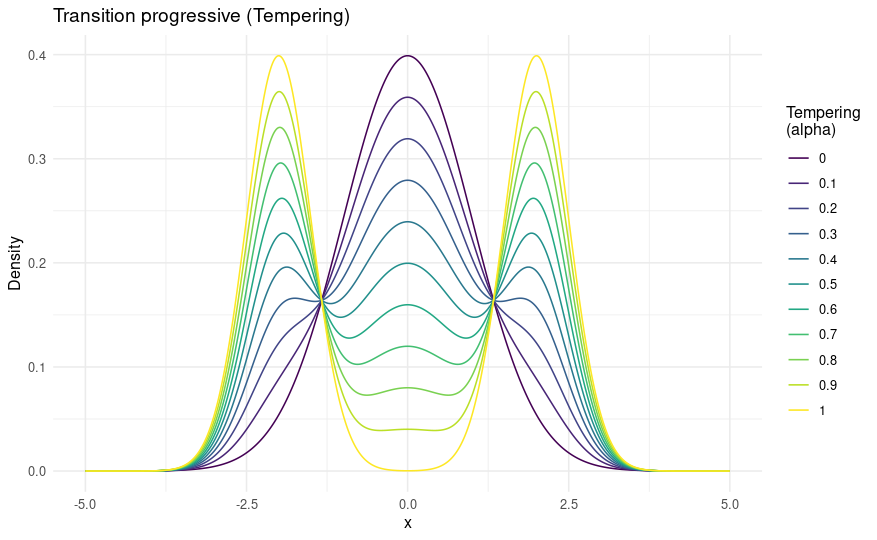
\includegraphics[scale=.716]{tempering.png}
Tempering strategies
\begin{itemize}
\item Data tempering :$n^{(\lambda)}_{v,s,a}\underset{\lambda\to 1}{\rightarrow} n\uparrow$.
\begin{itemize}
	\item minimum entropy of $n^{(\lambda)}_{v,s,\indexvec{a}}$
	\item at random
	\item by increasing observed positions ($v$ index).
\end{itemize}
\item $\bar\epsilon\to 1e^{-3}$
\item $\alpha_\tau\to 0$
\end{itemize}}
}
%%%%%%%%%%%%%%%%%%%%%%%%%%%%%%%%%%%%%%%%%%%%%%%%%%%
\def\blocksmc{
 \innerblock{Sequential Monte Carlo}{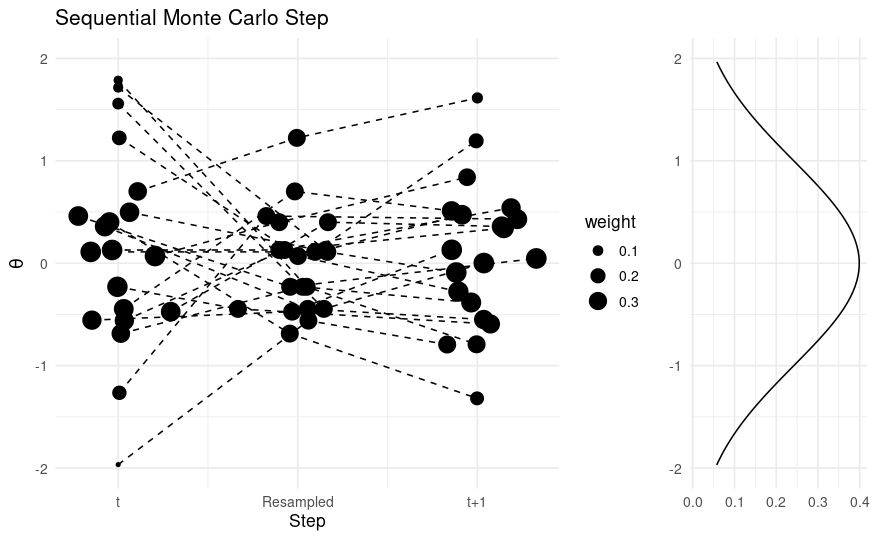
\includegraphics[scale=.724]{smc.png}}}
%%%%%%%%%%%%%%%%%%%%%%%%%%%%%%%%%%%%%%%%%%%%%%%%%%%
\def\blockmodels{
\innerblock{Alternative models}{
 
 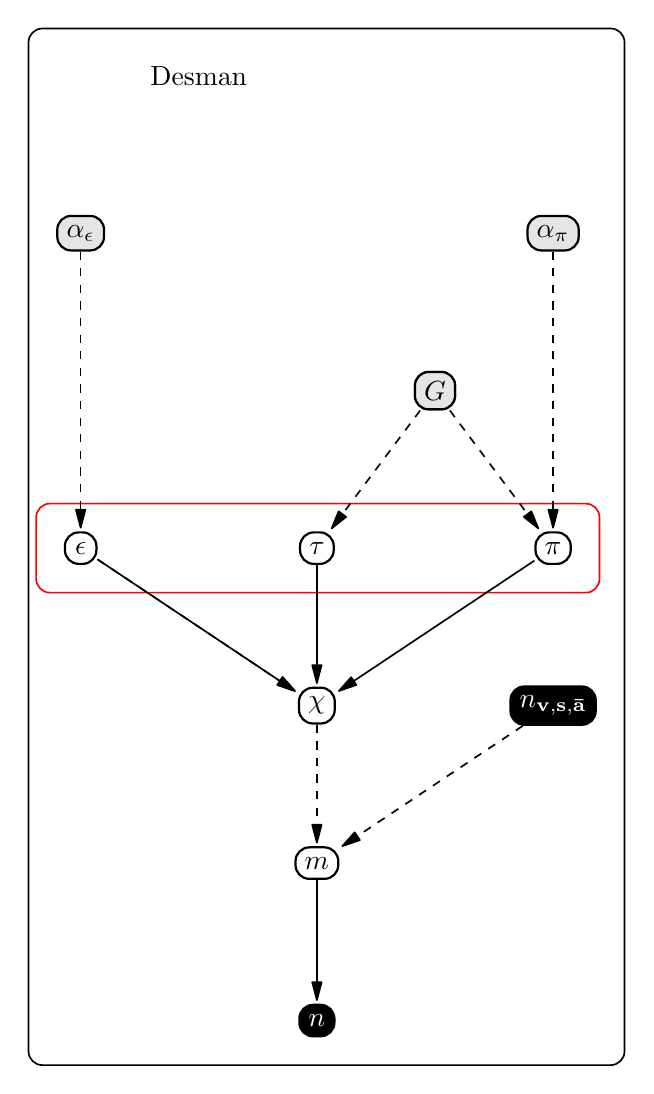
\begin{tikzpicture}[y=-2cm,x=3cm,
            > = {Stealth[inset=0pt,length=8pt,angle'=28,round]}, % arrow head style
            shorten > = 1pt, % don't touch arrow head to node
            auto,
%            node distance =1cm and 3cm, % distance between nodes
            semithick, % line style
            box/.style = {draw,red,inner sep=10pt,rounded corners=5pt}
        ]

        \tikzstyle{every state}=[
        rectangle,
        rounded corners=5pt,
            draw = black,
            thick,
            fill = white,
            minimum size = 4mm
        ]

 		\node at (1.5,1) (tt) {Desman};
        \node at (1.5,1) (blank) {};
        \node[state,fill=black!10] at (2.5,3) (G) {$G$};
        \node[state,fill=black!10] at (3,2) (alphapi) {$\alpha_\pi$};
        \node[state,fill=black!10] at (1,2) (alphaepsilon) {$\alpha_{\epsilon}$};
        \node[state] (tau) at (2,4) {$\tau$};
        \node[state] (epsilon) at (1,4) {$\epsilon$};
        \node[state] (pi) at (3,4) {$\pi$};
        \node[state] (chi) at (2,5) {$\chi$};
        %%\node (theta) at (0.5,4) {$\Theta$};
        \node[state,text=white,fill=black] (n) at (2,7) {$n$};
        \node[state,text=white,fill=black] (nvs) at (3,5)  {$n_{\indexvec{v},\indexvec{s},\indexsum{a}}$};
        \node[state] (m) at (2,6) {$\countdetail$};

         \node[box,fit=(tau) (pi) (epsilon)] {};
         
        \path[->,dashed] (alphapi) edge node {} (pi);
        \path[->,dashed] (alphaepsilon) edge node {} (epsilon);
        \path[->] (epsilon) edge node {} (chi);
        \path[->] (tau) edge node {} (chi);
        \path[->] (pi) edge node {} (chi);
        \path[->,dashed] (chi) edge node {} (m);
        \path[->,dashed] (epsilon) edge node {} (chi);
        \path[->,dashed] (nvs) edge node {} (m);
        \path[->,dashed] (G) edge node {} (tau);
        \path[->,dashed] (G) edge node {} (pi);
        \node[state,fill=black!10] at (2.5,3) (G) {$G$};
        \path[->] (m) edge node {} (n);
       
       
         \node[box,color=black,fit= (tt) (tau) (pi) (epsilon) (alphaepsilon) (m) (nvs) (n) (chi) (alphapi)] {};
        
    \end{tikzpicture}%
 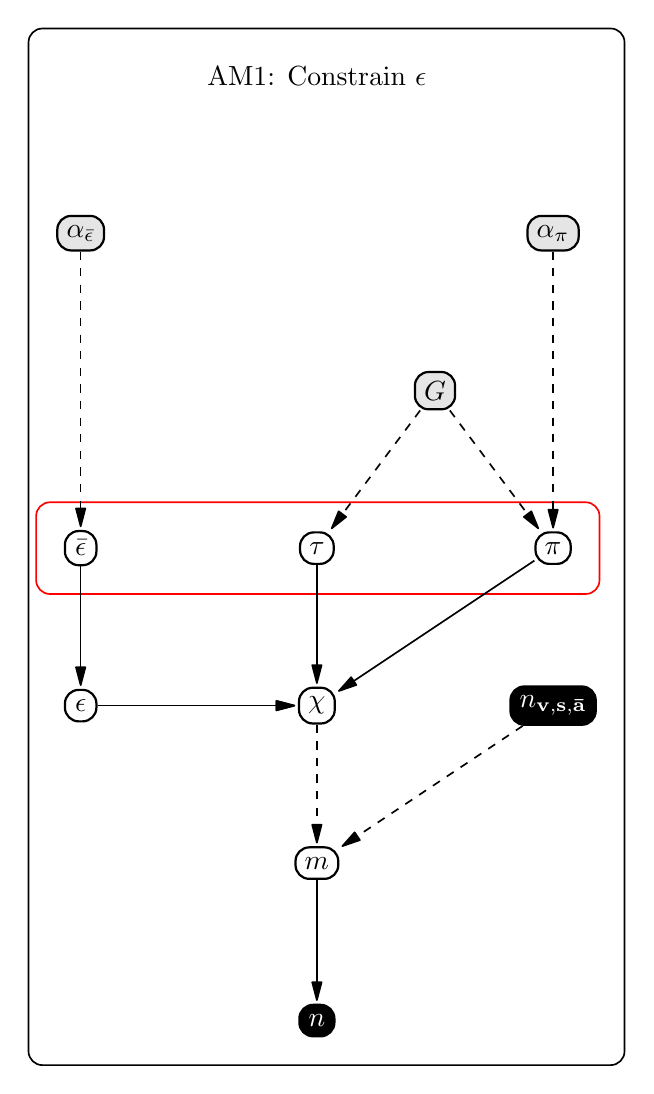
\begin{tikzpicture}[y=-2cm,x=3cm,
            > = {Stealth[inset=0pt,length=8pt,angle'=28,round]}, % arrow head style
            shorten > = 1pt, % don't touch arrow head to node
            auto,
%            node distance =1cm and 3cm, % distance between nodes
            semithick, % line style
            box/.style = {draw,red,inner sep=10pt,rounded corners=5pt}
        ]

        \tikzstyle{every state}=[
        rectangle,
        rounded corners=5pt,
            draw = black,
            thick,
            fill = white,
            minimum size = 4mm
        ]

        \node at (2,1) (tt) {AM1: Constrain $\epsilon$};
        \node at (1.5,1) (blank) {};

        \node[state,fill=black!10] at (2.5,3) (G) {$G$};
        \node[state,fill=black!10] at (3,2) (alphapi) {$\alpha_\pi$};
        \node[state,fill=black!10] at (1,2) (alphaepsilon) {$\alpha_{\bar\epsilon}$};
        \node[state] at (1,4) (barepsilon) {${\bar\epsilon}$};
        \node[state] (tau) at (2,4) {$\tau$};
        \node[state] (epsilon) at (1,5) {$\epsilon$};
        \node[state] (pi) at (3,4) {$\pi$};
        \node[state] (chi) at (2,5) {$\chi$};
        %%\node (theta) at (0.5,4) {$\Theta$};
        \node[state,text=white,fill=black] (n) at (2,7) {$n$};
        \node[state,text=white,fill=black] (nvs) at (3,5)  {$n_{\indexvec{v},\indexvec{s},\indexsum{a}}$};
        \node[state] (m) at (2,6) {$\countdetail$};

         \node[box,fit= (tau) (pi) (barepsilon)] {};
         
        \path[->,dashed] (alphapi) edge node {} (pi);
        \path[->,dashed] (alphaepsilon) edge node {} (barepsilon);
        \path[->] (barepsilon) edge node {} (epsilon);
        \path[->] (epsilon) edge node {} (chi);
        \path[->] (tau) edge node {} (chi);
        \path[->] (pi) edge node {} (chi);
        \path[->,dashed] (chi) edge node {} (m);
        \path[->] (epsilon) edge node {} (chi);
        \path[->,dashed] (nvs) edge node {} (m);
        \path[->] (m) edge node {} (n);
        \path[->,dashed] (G) edge node {} (tau);
        \path[->,dashed] (G) edge node {} (pi);
       
       
         \node[box,color=black,fit= (tt) (tau) (pi) (barepsilon) (alphaepsilon) (m) (nvs) (n) (chi) (alphapi)] {};
        
    \end{tikzpicture}%
 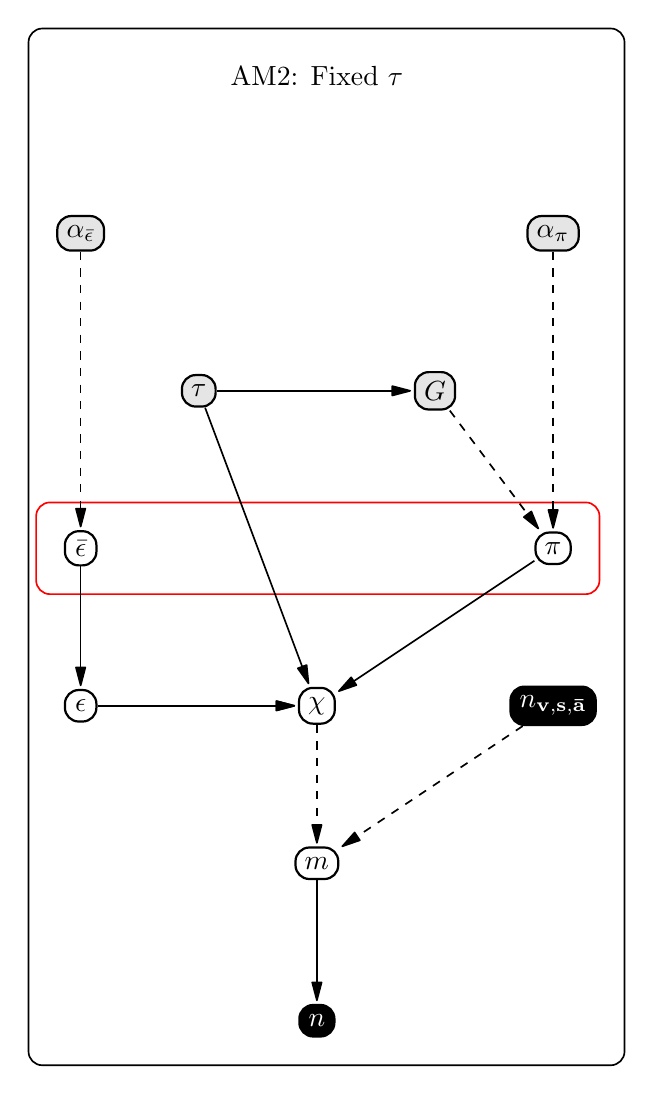
\begin{tikzpicture}[y=-2cm,x=3cm,
            > = {Stealth[inset=0pt,length=8pt,angle'=28,round]}, % arrow head style
            shorten > = 1pt, % don't touch arrow head to node
            auto,
%            node distance =1cm and 3cm, % distance between nodes
            semithick, % line style
            box/.style = {draw,red,inner sep=10pt,rounded corners=5pt}
        ]

        \tikzstyle{every state}=[
        rectangle,
        rounded corners=5pt,
            draw = black,
            thick,
            fill = white,
            minimum size = 4mm
        ]

        \node at (2,1) (tt) {AM2: Fixed $\tau$ };

        \node[state,fill=black!10] at (2.5,3) (G) {$G$};
        \node[state,fill=black!10] at (3,2) (alphapi) {$\alpha_\pi$};
        \node[state,fill=black!10] at (1,2) (alphaepsilon) {$\alpha_{\bar\epsilon}$};
        \node[state] at (1,4) (barepsilon) {${\bar\epsilon}$};
        \node[state,fill=black!10] (tau) at (1.5,3) {$\tau$};
        \node[state] (epsilon) at (1,5) {$\epsilon$};
        \node[state] (pi) at (3,4) {$\pi$};
        \node[state] (chi) at (2,5) {$\chi$};
        %\node (theta) at (0.5,4) {$\Theta$};
        \node[state,text=white,fill=black] (n) at (2,7) {$n$};
        \node[state,text=white,fill=black] (nvs) at (3,5)  {$n_{\indexvec{v},\indexvec{s},\indexsum{a}}$};
        \node[state] (m) at (2,6) {$\countdetail$};

         \node[box,fit=  (pi) (barepsilon)] {};
        \path[->,dashed] (alphapi) edge node {} (pi);
        \path[->,dashed] (alphaepsilon) edge node {} (barepsilon);
        \path[->] (barepsilon) edge node {} (epsilon);
        \path[->] (epsilon) edge node {} (chi);
        \path[->] (tau) edge node {} (chi);
        \path[->] (pi) edge node {} (chi);
        \path[->,dashed] (chi) edge node {} (m);
        \path[->] (epsilon) edge node {} (chi);
        \path[->,dashed] (nvs) edge node {} (m);
        \path[->] (m) edge node {} (n);
        \path[->] (tau) edge node {} (G);
        \path[->,dashed] (G) edge node {} (pi);
       
        
       
         \node[box,color=black,fit= (tt) (tau) (pi) (alphaepsilon) (alphapi) (m) (nvs) (n) (chi)] {};
    \end{tikzpicture}%
  \begin{tikzpicture}[y=-2cm,x=3cm,
            > = {Stealth[inset=0pt,length=8pt,angle'=28,round]}, % arrow head style
            shorten > = 1pt, % don't touch arrow head to node
            auto,
%            node distance =1cm and 3cm, % distance between nodes
            semithick, % line style
            box/.style = {draw,red,inner sep=10pt,rounded corners=5pt}
        ]

        \tikzstyle{every state}=[
        rectangle,
        rounded corners=5pt,
            draw = black,
            thick,
            fill = white,
            minimum size = 4mm
        ]


        \node at (2,0) (tt) {AM3: Relax $\rho$ };
        \node[state,fill=black!10] at (2.5,1.5) (G) {$G$};
        \node[state,fill=black!10] at (3,1) (alphapi) {$\alpha_\pi$};
        \node[state,fill=black!10] at (1.5,1) (alpharho) {$\alpha_\rho$};
        \node[state] (pi) at (3,3) {$\pi$};
        \node[state] (chi) at (1.75,4) {$\chi_{\indexvec{v},\indexvec{s},\indexvec{a},\indexsum{b},\indexvec{g}}$};
        \node[state] (rho) at (1.5,3) {$\tilde\rho$};
        \node[state] (tau) at (.5,4) {$\tau$};
        \node[state,text=white,fill=black] (n) at (2,6) {$n$};
        \node[state] (m) at (2,5) {$\countdetail_{\indexvec{v},\indexvec{s},\indexvec{a},\indexsum{b},\indexvec{g}}$};

        \node[state,text=white,fill=black] (nvs) at (3,4) {$n_{\indexvec{v},\indexvec{s},\indexsum{a}}$};
        
        \node[box,fit=(pi) (rho) ] {};
        \path[->,dashed] (alpharho) edge node {} (rho);
        \path[->,dashed] (alphapi) edge node {} (pi);
        \path[->] (pi) edge node {} (chi);
        \path[->] (rho) edge node {} (chi);
        \path[->,dashed] (chi) edge node {} (m);
        \path[->] (rho) edge node {} (tau);
        \path[->,dashed] (nvs) edge node {} (m);
        \path[->] (m) edge node {} (n);
        \path[->,dashed] (G) edge node {} (pi);
        \path[->,dashed] (G) edge node {} (rho);
        
        \node[box,color=black,fit= (tt) (tau) (pi) (alpharho) (alphaepsilon) (m) (nvs) (n) (chi)] {};
    \end{tikzpicture}%
 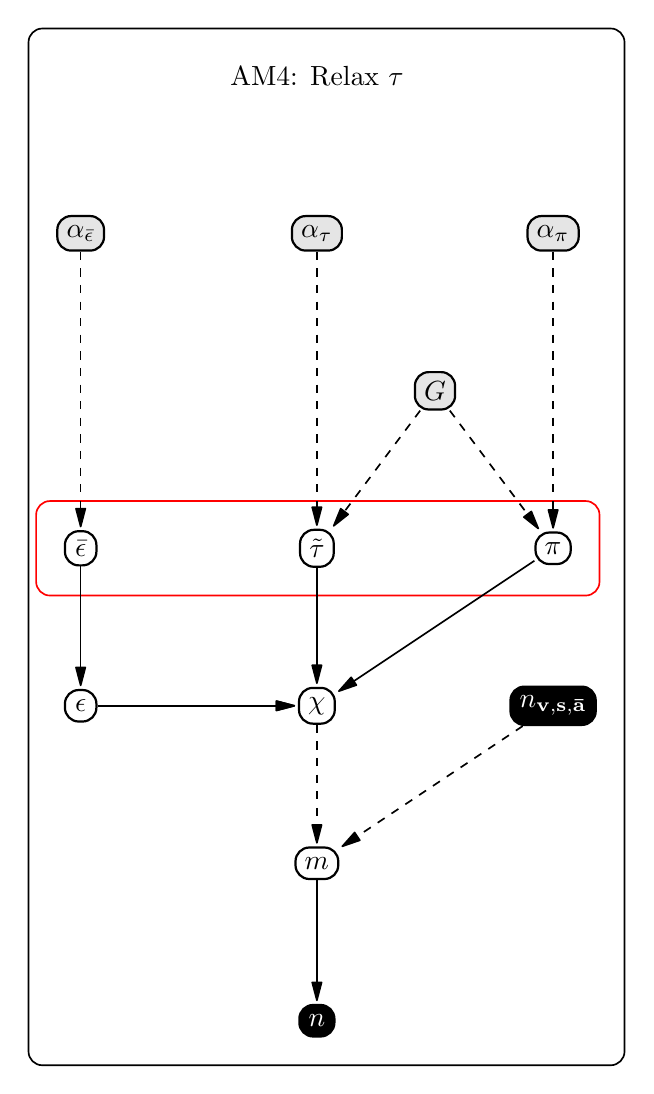
\begin{tikzpicture}[y=-2cm,x=3cm,
            > = {Stealth[inset=0pt,length=8pt,angle'=28,round]}, % arrow head style
            shorten > = 1pt, % don't touch arrow head to node
            auto,
%            node distance =1cm and 3cm, % distance between nodes
            semithick, % line style
            box/.style = {draw,red,inner sep=10pt,rounded corners=5pt}
        ]

        \tikzstyle{every state}=[
        rectangle,
        rounded corners=5pt,
            draw = black,
            thick,
            fill = white,
            minimum size = 4mm
        ]

        \node at (2,1) (tt) {AM4: Relax $\tau$ };
        \node at (1.5,1) (blank) {};

        \node[state,fill=black!10] at (2.5,3) (G) {$G$};
        \node[state,fill=black!10] at (2,2) (alphatau) {$\alpha_\tau$};
        \node[state,fill=black!10] at (3,2) (alphapi) {$\alpha_\pi$};
        \node[state,fill=black!10] at (1,2) (alphaepsilon) {$\alpha_{\bar\epsilon}$};
        \node[state] at (1,4) (barepsilon) {${\bar\epsilon}$};
        \node[state] (tau) at (2,4) {$\tilde\tau$};
        \node[state] (epsilon) at (1,5) {$\epsilon$};
        \node[state] (pi) at (3,4) {$\pi$};
        \node[state] (chi) at (2,5) {$\chi$};
        %\node (theta) at (0.5,4) {$\Theta$};
        \node[state,text=white,fill=black] (n) at (2,7) {$n$};
        \node[state,text=white,fill=black] (nvs) at (3,5)  {$n_{\indexvec{v},\indexvec{s},\indexsum{a}}$};
        \node[state] (m) at (2,6) {$\countdetail$};

         \node[box,fit= (tau) (pi) (barepsilon)] {};
        \path[->,dashed] (alphatau) edge node {} (tau);
        \path[->,dashed] (alphapi) edge node {} (pi);
        \path[->,dashed] (alphaepsilon) edge node {} (barepsilon);
        \path[->] (barepsilon) edge node {} (epsilon);
        \path[->] (epsilon) edge node {} (chi);
        \path[->] (tau) edge node {} (chi);
        \path[->] (pi) edge node {} (chi);
        \path[->,dashed] (chi) edge node {} (m);
        \path[->] (epsilon) edge node {} (chi);
        \path[->,dashed] (nvs) edge node {} (m);
        \path[->] (m) edge node {} (n);
        \path[->,dashed] (G) edge node {} (tau);
        \path[->,dashed] (G) edge node {} (pi);
       
         \node[box,color=black,fit= (tt) (tau) (pi) (barepsilon) (alphaepsilon) (m) (nvs) (n) (chi)] {};
        
    \end{tikzpicture}%
 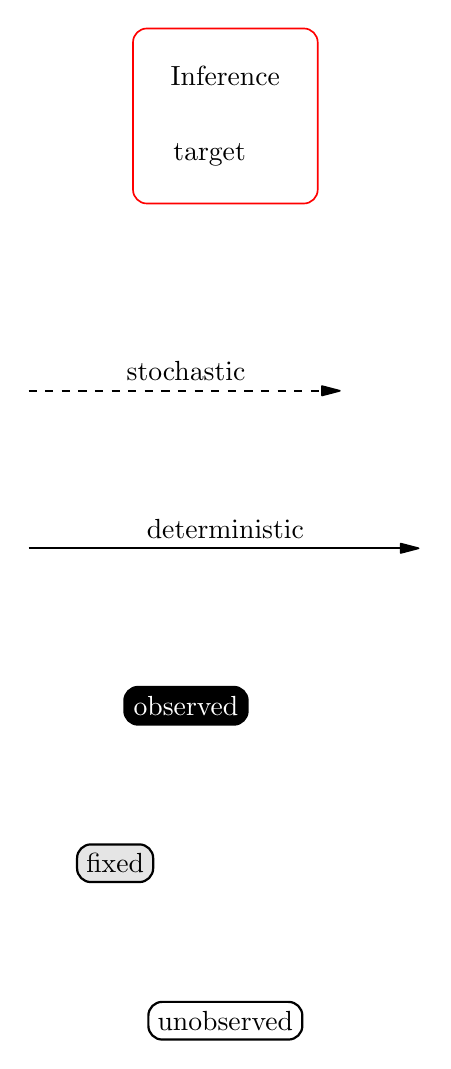
\begin{tikzpicture}[y=2cm,
            > = {Stealth[inset=0pt,length=8pt,angle'=28,round]}, % arrow head style
            shorten > = 1pt, % don't touch arrow head to node
            auto,
%            node distance =1cm and 3cm, % distance between nodes
            semithick, % line style
            box/.style = {draw,red,inner sep=10pt,rounded corners=5pt}
        ]

        \tikzstyle{every state}=[
        rectangle,
        rounded corners=5pt,
            draw = black,
            thick,
            fill = white,
            minimum size = 4mm
        ]

        \node[state,fill=black!10] at (1.1,1) (fixed) {fixed};
        \node[state] at (2.5,0)  (unobserved)  {unobserved};
        \node[state,text=white,fill=black ] at (2,2) (observed)  {observed};
        \path[->] (0,3) edge node {deterministic} (5,3);
        \path[->,dashed] (0,4) edge node {stochastic} (4,4);

        \node at (2.3,5.5) (theta1) {target};
        \node at (2.5,6) (theta2) {Inference};
        \node[box,fit=(theta1) (theta2)] {};
         \end{tikzpicture}
}}
%%%%%%%%%%%%%%%%%%%%%%%%%%%%%%%%%%%%%%%%%%%%%%%%%%%
\def\blockd{
\block{Alternative models and sampling strategies}{
\blockmodels
\innerblock{Relaxation}{
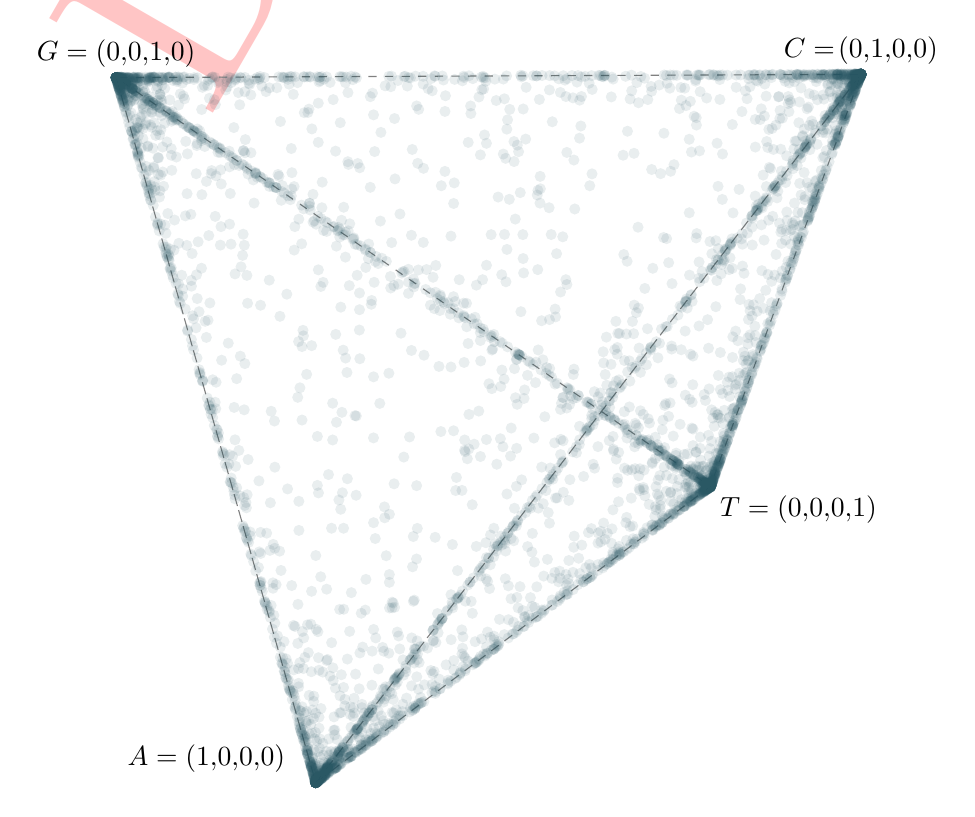
\begin{tikzpicture}[scale=10]


\begin{scope}[rotate around y=45,rotate around z=45]
 
% Draw the vertices of the tetrahedron

\coordinate (A) at (0, 0, 0);
\coordinate (C) at (1, 0, 0);
\coordinate (G) at (0.5, 0.866, 0);
\coordinate (T) at (0.5, 0.2887, 0.816);

%\foreach \p in {A,C,G,T}\fill[black] (\p) circle (0.02);

% Draw the edges of the cube
\draw[white!50!black, dashed]  (A) -- (C) -- (G) -- (A) -- (C) -- (T) -- (A) -- (T) -- (G) --  cycle;



    \pgfmathsetmacro{\alphaa}{0.1}       
       
\fill[color1,  opacity=\alphaa] (0.423,0.586,0.046) circle (.2pt);
         \fill[color1,  opacity=\alphaa] (0.984,0.027,0) circle (.2pt);
         \fill[color1,  opacity=\alphaa] (0.286,0.29,0.207) circle (.2pt);
         \fill[color1,  opacity=\alphaa] (0.842,0.106,0) circle (.2pt);
         \fill[color1,  opacity=\alphaa] (0.604,0.399,0.404) circle (.2pt);
         \fill[color1,  opacity=\alphaa] (0.093,0.02,0.057) circle (.2pt);
         \fill[color1,  opacity=\alphaa] (0,0,0) circle (.2pt);
         \fill[color1,  opacity=\alphaa] (0.231,0,0) circle (.2pt);
         \fill[color1,  opacity=\alphaa] (1,0,0) circle (.2pt);
         \fill[color1,  opacity=\alphaa] (0.36,0.556,0.003) circle (.2pt);
         \fill[color1,  opacity=\alphaa] (0.454,0.593,0.229) circle (.2pt);
         \fill[color1,  opacity=\alphaa] (0.506,0.85,0) circle (.2pt);
         \fill[color1,  opacity=\alphaa] (0.414,0.41,0.052) circle (.2pt);
         \fill[color1,  opacity=\alphaa] (0.533,0.269,0.762) circle (.2pt);
         \fill[color1,  opacity=\alphaa] (0.488,0.837,0) circle (.2pt);
         \fill[color1,  opacity=\alphaa] (0.001,0,0) circle (.2pt);
         \fill[color1,  opacity=\alphaa] (0.364,0.631,0) circle (.2pt);
         \fill[color1,  opacity=\alphaa] (0.495,0.836,0) circle (.2pt);
         \fill[color1,  opacity=\alphaa] (0.996,0.001,0) circle (.2pt);
         \fill[color1,  opacity=\alphaa] (0.999,0,0.001) circle (.2pt);
         \fill[color1,  opacity=\alphaa] (0.453,0.784,0) circle (.2pt);
         \fill[color1,  opacity=\alphaa] (0.405,0.235,0.66) circle (.2pt);
         \fill[color1,  opacity=\alphaa] (0.828,0.099,0.281) circle (.2pt);
         \fill[color1,  opacity=\alphaa] (0.648,0.186,0.526) circle (.2pt);
         \fill[color1,  opacity=\alphaa] (0.488,0.846,0) circle (.2pt);
         \fill[color1,  opacity=\alphaa] (0.47,0.438,0.499) circle (.2pt);
         \fill[color1,  opacity=\alphaa] (0.498,0.863,0) circle (.2pt);
         \fill[color1,  opacity=\alphaa] (0.006,0.01,0) circle (.2pt);
         \fill[color1,  opacity=\alphaa] (0.5,0.839,0.038) circle (.2pt);
         \fill[color1,  opacity=\alphaa] (0.605,0.051,0) circle (.2pt);
         \fill[color1,  opacity=\alphaa] (0.485,0.287,0.782) circle (.2pt);
         \fill[color1,  opacity=\alphaa] (0.516,0.502,0.418) circle (.2pt);
         \fill[color1,  opacity=\alphaa] (0.035,0.025,0.051) circle (.2pt);
         \fill[color1,  opacity=\alphaa] (0.5,0.289,0.816) circle (.2pt);
         \fill[color1,  opacity=\alphaa] (0.267,0.463,0) circle (.2pt);
         \fill[color1,  opacity=\alphaa] (0.5,0.289,0.816) circle (.2pt);
         \fill[color1,  opacity=\alphaa] (0.482,0.827,0) circle (.2pt);
         \fill[color1,  opacity=\alphaa] (0.5,0.298,0.804) circle (.2pt);
         \fill[color1,  opacity=\alphaa] (0.5,0.866,0) circle (.2pt);
         \fill[color1,  opacity=\alphaa] (0.5,0.289,0.816) circle (.2pt);
         \fill[color1,  opacity=\alphaa] (0.844,0.092,0.252) circle (.2pt);
         \fill[color1,  opacity=\alphaa] (0.476,0.583,0.341) circle (.2pt);
         \fill[color1,  opacity=\alphaa] (0.46,0.777,0.029) circle (.2pt);
         \fill[color1,  opacity=\alphaa] (0.996,0.007,0) circle (.2pt);
         \fill[color1,  opacity=\alphaa] (0.392,0.498,0.256) circle (.2pt);
         \fill[color1,  opacity=\alphaa] (0.977,0.013,0.038) circle (.2pt);
         \fill[color1,  opacity=\alphaa] (0.95,0.032,0.077) circle (.2pt);
         \fill[color1,  opacity=\alphaa] (0.436,0.611,0.002) circle (.2pt);
         \fill[color1,  opacity=\alphaa] (0.025,0.029,0.019) circle (.2pt);
         \fill[color1,  opacity=\alphaa] (0.952,0.028,0.079) circle (.2pt);
         \fill[color1,  opacity=\alphaa] (0.975,0.004,0.011) circle (.2pt);
         \fill[color1,  opacity=\alphaa] (0.006,0.002,0.006) circle (.2pt);
         \fill[color1,  opacity=\alphaa] (0.52,0.261,0.738) circle (.2pt);
         \fill[color1,  opacity=\alphaa] (0.319,0.184,0.521) circle (.2pt);
         \fill[color1,  opacity=\alphaa] (0.382,0.238,0.595) circle (.2pt);
         \fill[color1,  opacity=\alphaa] (0.207,0.357,0) circle (.2pt);
         \fill[color1,  opacity=\alphaa] (0.5,0.851,0.022) circle (.2pt);
         \fill[color1,  opacity=\alphaa] (0.575,0.22,0.616) circle (.2pt);
         \fill[color1,  opacity=\alphaa] (0.489,0.804,0.06) circle (.2pt);
         \fill[color1,  opacity=\alphaa] (0.968,0.006,0) circle (.2pt);
         \fill[color1,  opacity=\alphaa] (0.403,0,0) circle (.2pt);
         \fill[color1,  opacity=\alphaa] (0.008,0,0) circle (.2pt);
         \fill[color1,  opacity=\alphaa] (0.523,0.275,0.778) circle (.2pt);
         \fill[color1,  opacity=\alphaa] (0.5,0.474,0.554) circle (.2pt);
         \fill[color1,  opacity=\alphaa] (0.516,0.822,0.022) circle (.2pt);
         \fill[color1,  opacity=\alphaa] (0.021,0.001,0.003) circle (.2pt);
         \fill[color1,  opacity=\alphaa] (0.5,0.866,0) circle (.2pt);
         \fill[color1,  opacity=\alphaa] (0.339,0,0) circle (.2pt);
         \fill[color1,  opacity=\alphaa] (0.505,0.856,0.002) circle (.2pt);
         \fill[color1,  opacity=\alphaa] (0.002,0,0) circle (.2pt);
         \fill[color1,  opacity=\alphaa] (0.132,0.044,0.125) circle (.2pt);
         \fill[color1,  opacity=\alphaa] (0.508,0.851,0) circle (.2pt);
         \fill[color1,  opacity=\alphaa] (0,0,0) circle (.2pt);
         \fill[color1,  opacity=\alphaa] (0.831,0.29,0.003) circle (.2pt);
         \fill[color1,  opacity=\alphaa] (0,0,0) circle (.2pt);
         \fill[color1,  opacity=\alphaa] (0.502,0.301,0.793) circle (.2pt);
         \fill[color1,  opacity=\alphaa] (0.598,0.67,0.001) circle (.2pt);
         \fill[color1,  opacity=\alphaa] (0.5,0.846,0.028) circle (.2pt);
         \fill[color1,  opacity=\alphaa] (0.979,0.037,0) circle (.2pt);
         \fill[color1,  opacity=\alphaa] (0.548,0.78,0) circle (.2pt);
         \fill[color1,  opacity=\alphaa] (0.528,0.273,0.771) circle (.2pt);
         \fill[color1,  opacity=\alphaa] (0.445,0.769,0) circle (.2pt);
         \fill[color1,  opacity=\alphaa] (1,0,0) circle (.2pt);
         \fill[color1,  opacity=\alphaa] (0.461,0.264,0.748) circle (.2pt);
         \fill[color1,  opacity=\alphaa] (0.486,0.779,0.087) circle (.2pt);
         \fill[color1,  opacity=\alphaa] (0.074,0.018,0.034) circle (.2pt);
         \fill[color1,  opacity=\alphaa] (0.205,0.014,0.04) circle (.2pt);
         \fill[color1,  opacity=\alphaa] (0.501,0.288,0.815) circle (.2pt);
         \fill[color1,  opacity=\alphaa] (0.901,0.171,0) circle (.2pt);
         \fill[color1,  opacity=\alphaa] (0.5,0.305,0.793) circle (.2pt);
         \fill[color1,  opacity=\alphaa] (0.476,0.275,0.777) circle (.2pt);
         \fill[color1,  opacity=\alphaa] (0.563,0.749,0.011) circle (.2pt);
         \fill[color1,  opacity=\alphaa] (0.194,0.005,0.014) circle (.2pt);
         \fill[color1,  opacity=\alphaa] (0.5,0.289,0.816) circle (.2pt);
         \fill[color1,  opacity=\alphaa] (0.984,0,0) circle (.2pt);
         \fill[color1,  opacity=\alphaa] (0.97,0.016,0.013) circle (.2pt);
         \fill[color1,  opacity=\alphaa] (0.494,0.855,0) circle (.2pt);
         \fill[color1,  opacity=\alphaa] (0.497,0.287,0.811) circle (.2pt);
         \fill[color1,  opacity=\alphaa] (0.883,0.202,0) circle (.2pt);
         \fill[color1,  opacity=\alphaa] (0.305,0.055,0.001) circle (.2pt);
         \fill[color1,  opacity=\alphaa] (0.356,0.211,0.574) circle (.2pt);
         \fill[color1,  opacity=\alphaa] (0.02,0.035,0) circle (.2pt);
         \fill[color1,  opacity=\alphaa] (0.796,0.117,0.33) circle (.2pt);
         \fill[color1,  opacity=\alphaa] (0.391,0.161,0.43) circle (.2pt);
         \fill[color1,  opacity=\alphaa] (0.099,0.001,0) circle (.2pt);
         \fill[color1,  opacity=\alphaa] (0,0,0) circle (.2pt);
         \fill[color1,  opacity=\alphaa] (0.483,0.411,0.603) circle (.2pt);
         \fill[color1,  opacity=\alphaa] (0.5,0.289,0.816) circle (.2pt);
         \fill[color1,  opacity=\alphaa] (0.499,0.288,0.815) circle (.2pt);
         \fill[color1,  opacity=\alphaa] (0.499,0.864,0) circle (.2pt);
         \fill[color1,  opacity=\alphaa] (0.496,0.285,0.807) circle (.2pt);
         \fill[color1,  opacity=\alphaa] (0.493,0.852,0.002) circle (.2pt);
         \fill[color1,  opacity=\alphaa] (0.501,0.296,0.803) circle (.2pt);
         \fill[color1,  opacity=\alphaa] (0.155,0.26,0) circle (.2pt);
         \fill[color1,  opacity=\alphaa] (0.493,0.285,0.806) circle (.2pt);
         \fill[color1,  opacity=\alphaa] (0.581,0.14,0.377) circle (.2pt);
         \fill[color1,  opacity=\alphaa] (0.738,0,0) circle (.2pt);
         \fill[color1,  opacity=\alphaa] (0.655,0.199,0.563) circle (.2pt);
         \fill[color1,  opacity=\alphaa] (0.492,0.694,0.221) circle (.2pt);
         \fill[color1,  opacity=\alphaa] (0.502,0.86,0.004) circle (.2pt);
         \fill[color1,  opacity=\alphaa] (0.725,0.023,0.066) circle (.2pt);
         \fill[color1,  opacity=\alphaa] (0.029,0.049,0) circle (.2pt);
         \fill[color1,  opacity=\alphaa] (0.262,0,0) circle (.2pt);
         \fill[color1,  opacity=\alphaa] (0.382,0.368,0.414) circle (.2pt);
         \fill[color1,  opacity=\alphaa] (0.999,0.001,0.002) circle (.2pt);
         \fill[color1,  opacity=\alphaa] (0.5,0.313,0.783) circle (.2pt);
         \fill[color1,  opacity=\alphaa] (0.999,0,0) circle (.2pt);
         \fill[color1,  opacity=\alphaa] (0.496,0.858,0.001) circle (.2pt);
         \fill[color1,  opacity=\alphaa] (0.71,0.171,0.469) circle (.2pt);
         \fill[color1,  opacity=\alphaa] (0.025,0.014,0.041) circle (.2pt);
         \fill[color1,  opacity=\alphaa] (0.049,0,0) circle (.2pt);
         \fill[color1,  opacity=\alphaa] (0.439,0.15,0.424) circle (.2pt);
         \fill[color1,  opacity=\alphaa] (0.261,0.151,0.418) circle (.2pt);
         \fill[color1,  opacity=\alphaa] (0,0,0) circle (.2pt);
         \fill[color1,  opacity=\alphaa] (0.5,0.864,0.002) circle (.2pt);
         \fill[color1,  opacity=\alphaa] (0.347,0.427,0.242) circle (.2pt);
         \fill[color1,  opacity=\alphaa] (0.95,0.029,0.081) circle (.2pt);
         \fill[color1,  opacity=\alphaa] (1,0,0) circle (.2pt);
         \fill[color1,  opacity=\alphaa] (0.988,0.02,0) circle (.2pt);
         \fill[color1,  opacity=\alphaa] (0.784,0.124,0.35) circle (.2pt);
         \fill[color1,  opacity=\alphaa] (0.468,0.274,0.759) circle (.2pt);
         \fill[color1,  opacity=\alphaa] (0.286,0.093,0.263) circle (.2pt);
         \fill[color1,  opacity=\alphaa] (0.493,0.847,0.009) circle (.2pt);
         \fill[color1,  opacity=\alphaa] (0.927,0,0) circle (.2pt);
         \fill[color1,  opacity=\alphaa] (0.429,0,0) circle (.2pt);
         \fill[color1,  opacity=\alphaa] (0.916,0.047,0.133) circle (.2pt);
         \fill[color1,  opacity=\alphaa] (0.613,0,0.001) circle (.2pt);
         \fill[color1,  opacity=\alphaa] (0.5,0.327,0.763) circle (.2pt);
         \fill[color1,  opacity=\alphaa] (0.963,0.007,0) circle (.2pt);
         \fill[color1,  opacity=\alphaa] (0.534,0.268,0.759) circle (.2pt);
         \fill[color1,  opacity=\alphaa] (0.483,0.309,0.747) circle (.2pt);
         \fill[color1,  opacity=\alphaa] (0.499,0.865,0) circle (.2pt);
         \fill[color1,  opacity=\alphaa] (0.285,0.452,0.057) circle (.2pt);
         \fill[color1,  opacity=\alphaa] (0.848,0.088,0.247) circle (.2pt);
         \fill[color1,  opacity=\alphaa] (0.118,0.203,0.003) circle (.2pt);
         \fill[color1,  opacity=\alphaa] (1,0,0) circle (.2pt);
         \fill[color1,  opacity=\alphaa] (0.261,0.018,0.05) circle (.2pt);
         \fill[color1,  opacity=\alphaa] (0.5,0.866,0) circle (.2pt);
         \fill[color1,  opacity=\alphaa] (0.5,0.339,0.744) circle (.2pt);
         \fill[color1,  opacity=\alphaa] (0.066,0.113,0) circle (.2pt);
         \fill[color1,  opacity=\alphaa] (0.507,0.285,0.806) circle (.2pt);
         \fill[color1,  opacity=\alphaa] (0.023,0.004,0.01) circle (.2pt);
         \fill[color1,  opacity=\alphaa] (0.139,0.148,0) circle (.2pt);
         \fill[color1,  opacity=\alphaa] (0.507,0.332,0.74) circle (.2pt);
         \fill[color1,  opacity=\alphaa] (0.5,0.865,0.001) circle (.2pt);
         \fill[color1,  opacity=\alphaa] (0.5,0.301,0.799) circle (.2pt);
         \fill[color1,  opacity=\alphaa] (0.012,0.021,0) circle (.2pt);
         \fill[color1,  opacity=\alphaa] (0.459,0.767,0) circle (.2pt);
         \fill[color1,  opacity=\alphaa] (0.779,0.128,0.36) circle (.2pt);
         \fill[color1,  opacity=\alphaa] (0.5,0.699,0.236) circle (.2pt);
         \fill[color1,  opacity=\alphaa] (0.868,0.229,0) circle (.2pt);
         \fill[color1,  opacity=\alphaa] (0.004,0,0) circle (.2pt);
         \fill[color1,  opacity=\alphaa] (0.5,0.663,0.288) circle (.2pt);
         \fill[color1,  opacity=\alphaa] (0.496,0.507,0.498) circle (.2pt);
         \fill[color1,  opacity=\alphaa] (0.184,0.289,0.043) circle (.2pt);
         \fill[color1,  opacity=\alphaa] (0.5,0.863,0.004) circle (.2pt);
         \fill[color1,  opacity=\alphaa] (0.955,0.032,0.066) circle (.2pt);
         \fill[color1,  opacity=\alphaa] (0.484,0.838,0.002) circle (.2pt);
         \fill[color1,  opacity=\alphaa] (0.043,0.074,0) circle (.2pt);
         \fill[color1,  opacity=\alphaa] (0.501,0.31,0.784) circle (.2pt);
         \fill[color1,  opacity=\alphaa] (0.992,0.009,0) circle (.2pt);
         \fill[color1,  opacity=\alphaa] (0.491,0.851,0) circle (.2pt);
         \fill[color1,  opacity=\alphaa] (0.499,0.291,0.809) circle (.2pt);
         \fill[color1,  opacity=\alphaa] (0,0,0) circle (.2pt);
         \fill[color1,  opacity=\alphaa] (0.047,0.012,0.033) circle (.2pt);
         \fill[color1,  opacity=\alphaa] (0.961,0.067,0) circle (.2pt);
         \fill[color1,  opacity=\alphaa] (0.502,0.287,0.813) circle (.2pt);
         \fill[color1,  opacity=\alphaa] (0.499,0.288,0.814) circle (.2pt);
         \fill[color1,  opacity=\alphaa] (0.181,0.161,0) circle (.2pt);
         \fill[color1,  opacity=\alphaa] (0.455,0.783,0.001) circle (.2pt);
         \fill[color1,  opacity=\alphaa] (0.875,0,0) circle (.2pt);
         \fill[color1,  opacity=\alphaa] (0.505,0.304,0.782) circle (.2pt);
         \fill[color1,  opacity=\alphaa] (0.66,0.221,0.519) circle (.2pt);
         \fill[color1,  opacity=\alphaa] (0.564,0.252,0.712) circle (.2pt);
         \fill[color1,  opacity=\alphaa] (0.5,0.289,0.816) circle (.2pt);
         \fill[color1,  opacity=\alphaa] (0.5,0.289,0.816) circle (.2pt);
         \fill[color1,  opacity=\alphaa] (0.667,0.325,0.355) circle (.2pt);
         \fill[color1,  opacity=\alphaa] (1,0,0) circle (.2pt);
         \fill[color1,  opacity=\alphaa] (0.406,0.454,0.29) circle (.2pt);
         \fill[color1,  opacity=\alphaa] (0.55,0.776,0.004) circle (.2pt);
         \fill[color1,  opacity=\alphaa] (0.309,0.179,0.505) circle (.2pt);
         \fill[color1,  opacity=\alphaa] (0.5,0.861,0.007) circle (.2pt);
         \fill[color1,  opacity=\alphaa] (0.47,0.723,0.127) circle (.2pt);
         \fill[color1,  opacity=\alphaa] (0.061,0.03,0.083) circle (.2pt);
         \fill[color1,  opacity=\alphaa] (1,0,0) circle (.2pt);
         \fill[color1,  opacity=\alphaa] (0.5,0.288,0.816) circle (.2pt);
         \fill[color1,  opacity=\alphaa] (0.001,0,0) circle (.2pt);
         \fill[color1,  opacity=\alphaa] (0.5,0.865,0) circle (.2pt);
         \fill[color1,  opacity=\alphaa] (0.883,0.203,0) circle (.2pt);
         \fill[color1,  opacity=\alphaa] (0.224,0,0) circle (.2pt);
         \fill[color1,  opacity=\alphaa] (0.849,0.234,0) circle (.2pt);
         \fill[color1,  opacity=\alphaa] (0.484,0,0) circle (.2pt);
         \fill[color1,  opacity=\alphaa] (0.732,0.154,0.437) circle (.2pt);
         \fill[color1,  opacity=\alphaa] (0.998,0.001,0.004) circle (.2pt);
         \fill[color1,  opacity=\alphaa] (0.46,0.424,0.526) circle (.2pt);
         \fill[color1,  opacity=\alphaa] (0.524,0.825,0) circle (.2pt);
         \fill[color1,  opacity=\alphaa] (0.531,0.026,0.054) circle (.2pt);
         \fill[color1,  opacity=\alphaa] (0.022,0.001,0) circle (.2pt);
         \fill[color1,  opacity=\alphaa] (0.733,0.037,0.099) circle (.2pt);
         \fill[color1,  opacity=\alphaa] (0.5,0.339,0.745) circle (.2pt);
         \fill[color1,  opacity=\alphaa] (0.993,0.013,0) circle (.2pt);
         \fill[color1,  opacity=\alphaa] (0.5,0.857,0.013) circle (.2pt);
         \fill[color1,  opacity=\alphaa] (0.995,0.001,0.001) circle (.2pt);
         \fill[color1,  opacity=\alphaa] (0.075,0.103,0.039) circle (.2pt);
         \fill[color1,  opacity=\alphaa] (0.994,0.003,0.009) circle (.2pt);
         \fill[color1,  opacity=\alphaa] (0.855,0.021,0) circle (.2pt);
         \fill[color1,  opacity=\alphaa] (0.5,0.856,0.014) circle (.2pt);
         \fill[color1,  opacity=\alphaa] (0.995,0.003,0.008) circle (.2pt);
         \fill[color1,  opacity=\alphaa] (1,0,0) circle (.2pt);
         \fill[color1,  opacity=\alphaa] (0.002,0.001,0) circle (.2pt);
         \fill[color1,  opacity=\alphaa] (0.994,0,0.001) circle (.2pt);
         \fill[color1,  opacity=\alphaa] (0.493,0.281,0.794) circle (.2pt);
         \fill[color1,  opacity=\alphaa] (0.825,0.303,0) circle (.2pt);
         \fill[color1,  opacity=\alphaa] (0.501,0.859,0.008) circle (.2pt);
         \fill[color1,  opacity=\alphaa] (0.496,0.286,0.808) circle (.2pt);
         \fill[color1,  opacity=\alphaa] (0.497,0.283,0.799) circle (.2pt);
         \fill[color1,  opacity=\alphaa] (0.501,0.288,0.814) circle (.2pt);
         \fill[color1,  opacity=\alphaa] (0.502,0.298,0.798) circle (.2pt);
         \fill[color1,  opacity=\alphaa] (0.229,0.059,0.017) circle (.2pt);
         \fill[color1,  opacity=\alphaa] (0.5,0.858,0.011) circle (.2pt);
         \fill[color1,  opacity=\alphaa] (0.5,0.866,0) circle (.2pt);
         \fill[color1,  opacity=\alphaa] (0.17,0.06,0) circle (.2pt);
         \fill[color1,  opacity=\alphaa] (0.398,0.686,0.006) circle (.2pt);
         \fill[color1,  opacity=\alphaa] (0.949,0.071,0) circle (.2pt);
         \fill[color1,  opacity=\alphaa] (0.5,0.289,0.816) circle (.2pt);
         \fill[color1,  opacity=\alphaa] (0.976,0.03,0) circle (.2pt);
         \fill[color1,  opacity=\alphaa] (0.286,0.109,0.003) circle (.2pt);
         \fill[color1,  opacity=\alphaa] (0.002,0.001,0.002) circle (.2pt);
         \fill[color1,  opacity=\alphaa] (0.345,0.559,0) circle (.2pt);
         \fill[color1,  opacity=\alphaa] (0.456,0.633,0.219) circle (.2pt);
         \fill[color1,  opacity=\alphaa] (0.499,0.833,0.045) circle (.2pt);
         \fill[color1,  opacity=\alphaa] (0.01,0.005,0.002) circle (.2pt);
         \fill[color1,  opacity=\alphaa] (0.491,0.33,0.735) circle (.2pt);
         \fill[color1,  opacity=\alphaa] (0.554,0.752,0) circle (.2pt);
         \fill[color1,  opacity=\alphaa] (0.493,0.854,0) circle (.2pt);
         \fill[color1,  opacity=\alphaa] (0.999,0.001,0) circle (.2pt);
         \fill[color1,  opacity=\alphaa] (0.984,0.028,0) circle (.2pt);
         \fill[color1,  opacity=\alphaa] (0.999,0,0) circle (.2pt);
         \fill[color1,  opacity=\alphaa] (0.071,0.041,0.117) circle (.2pt);
         \fill[color1,  opacity=\alphaa] (0,0,0) circle (.2pt);
         \fill[color1,  opacity=\alphaa] (0.572,0.649,0.13) circle (.2pt);
         \fill[color1,  opacity=\alphaa] (0.406,0.235,0.662) circle (.2pt);
         \fill[color1,  opacity=\alphaa] (0.001,0.001,0.001) circle (.2pt);
         \fill[color1,  opacity=\alphaa] (0.998,0.001,0.003) circle (.2pt);
         \fill[color1,  opacity=\alphaa] (0.334,0,0) circle (.2pt);
         \fill[color1,  opacity=\alphaa] (0.989,0,0) circle (.2pt);
         \fill[color1,  opacity=\alphaa] (0.716,0.485,0.005) circle (.2pt);
         \fill[color1,  opacity=\alphaa] (0.002,0.004,0) circle (.2pt);
         \fill[color1,  opacity=\alphaa] (0.948,0.033,0.08) circle (.2pt);
         \fill[color1,  opacity=\alphaa] (0.996,0.002,0.007) circle (.2pt);
         \fill[color1,  opacity=\alphaa] (0.03,0.048,0) circle (.2pt);
         \fill[color1,  opacity=\alphaa] (0.503,0.335,0.744) circle (.2pt);
         \fill[color1,  opacity=\alphaa] (0.241,0.001,0) circle (.2pt);
         \fill[color1,  opacity=\alphaa] (0.063,0,0) circle (.2pt);
         \fill[color1,  opacity=\alphaa] (0.5,0.289,0.816) circle (.2pt);
         \fill[color1,  opacity=\alphaa] (0,0,0) circle (.2pt);
         \fill[color1,  opacity=\alphaa] (0.026,0,0) circle (.2pt);
         \fill[color1,  opacity=\alphaa] (0.021,0.037,0) circle (.2pt);
         \fill[color1,  opacity=\alphaa] (0.511,0.836,0.013) circle (.2pt);
         \fill[color1,  opacity=\alphaa] (0.953,0.027,0.076) circle (.2pt);
         \fill[color1,  opacity=\alphaa] (0.013,0,0) circle (.2pt);
         \fill[color1,  opacity=\alphaa] (0.452,0.288,0.7) circle (.2pt);
         \fill[color1,  opacity=\alphaa] (0.004,0.002,0.006) circle (.2pt);
         \fill[color1,  opacity=\alphaa] (0.455,0.055,0) circle (.2pt);
         \fill[color1,  opacity=\alphaa] (0.775,0.13,0.367) circle (.2pt);
         \fill[color1,  opacity=\alphaa] (0.5,0.289,0.816) circle (.2pt);
         \fill[color1,  opacity=\alphaa] (0.841,0,0) circle (.2pt);
         \fill[color1,  opacity=\alphaa] (0.732,0.004,0.009) circle (.2pt);
         \fill[color1,  opacity=\alphaa] (0.488,0.282,0.797) circle (.2pt);
         \fill[color1,  opacity=\alphaa] (0.003,0.005,0) circle (.2pt);
         \fill[color1,  opacity=\alphaa] (0.5,0.866,0.001) circle (.2pt);
         \fill[color1,  opacity=\alphaa] (0.513,0.281,0.796) circle (.2pt);
         \fill[color1,  opacity=\alphaa] (0.497,0.31,0.778) circle (.2pt);
         \fill[color1,  opacity=\alphaa] (0.83,0.289,0.007) circle (.2pt);
         \fill[color1,  opacity=\alphaa] (0.501,0.288,0.814) circle (.2pt);
         \fill[color1,  opacity=\alphaa] (0.5,0.29,0.815) circle (.2pt);
         \fill[color1,  opacity=\alphaa] (0.971,0.02,0.041) circle (.2pt);
         \fill[color1,  opacity=\alphaa] (0,0,0) circle (.2pt);
         \fill[color1,  opacity=\alphaa] (0.513,0.82,0.034) circle (.2pt);
         \fill[color1,  opacity=\alphaa] (0.518,0.67,0.234) circle (.2pt);
         \fill[color1,  opacity=\alphaa] (0.989,0.006,0.018) circle (.2pt);
         \fill[color1,  opacity=\alphaa] (1,0,0) circle (.2pt);
         \fill[color1,  opacity=\alphaa] (0.5,0.854,0.017) circle (.2pt);
         \fill[color1,  opacity=\alphaa] (0.501,0.797,0.059) circle (.2pt);
         \fill[color1,  opacity=\alphaa] (0.783,0.139,0.335) circle (.2pt);
         \fill[color1,  opacity=\alphaa] (0.194,0.135,0.01) circle (.2pt);
         \fill[color1,  opacity=\alphaa] (0.504,0.86,0) circle (.2pt);
         \fill[color1,  opacity=\alphaa] (0.915,0.049,0.139) circle (.2pt);
         \fill[color1,  opacity=\alphaa] (0.006,0.003,0.01) circle (.2pt);
         \fill[color1,  opacity=\alphaa] (0.5,0.393,0.669) circle (.2pt);
         \fill[color1,  opacity=\alphaa] (0.001,0,0.001) circle (.2pt);
         \fill[color1,  opacity=\alphaa] (0.916,0.089,0.065) circle (.2pt);
         \fill[color1,  opacity=\alphaa] (0.003,0,0) circle (.2pt);
         \fill[color1,  opacity=\alphaa] (0.552,0.216,0.612) circle (.2pt);
         \fill[color1,  opacity=\alphaa] (0.987,0.023,0) circle (.2pt);
         \fill[color1,  opacity=\alphaa] (0.883,0,0) circle (.2pt);
         \fill[color1,  opacity=\alphaa] (0.362,0,0) circle (.2pt);
         \fill[color1,  opacity=\alphaa] (0.952,0.003,0.003) circle (.2pt);
         \fill[color1,  opacity=\alphaa] (0.091,0.151,0.009) circle (.2pt);
         \fill[color1,  opacity=\alphaa] (0.426,0.733,0.007) circle (.2pt);
         \fill[color1,  opacity=\alphaa] (0.5,0.861,0.007) circle (.2pt);
         \fill[color1,  opacity=\alphaa] (0.5,0.289,0.816) circle (.2pt);
         \fill[color1,  opacity=\alphaa] (0.62,0.658,0) circle (.2pt);
         \fill[color1,  opacity=\alphaa] (0.785,0.341,0.044) circle (.2pt);
         \fill[color1,  opacity=\alphaa] (0.004,0.007,0) circle (.2pt);
         \fill[color1,  opacity=\alphaa] (0.702,0.185,0.416) circle (.2pt);
         \fill[color1,  opacity=\alphaa] (0.071,0.041,0.116) circle (.2pt);
         \fill[color1,  opacity=\alphaa] (0.498,0.311,0.781) circle (.2pt);
         \fill[color1,  opacity=\alphaa] (0.499,0.86,0.006) circle (.2pt);
         \fill[color1,  opacity=\alphaa] (0.508,0.85,0) circle (.2pt);
         \fill[color1,  opacity=\alphaa] (0.006,0,0) circle (.2pt);
         \fill[color1,  opacity=\alphaa] (0.523,0.826,0) circle (.2pt);
         \fill[color1,  opacity=\alphaa] (0.001,0,0) circle (.2pt);
         \fill[color1,  opacity=\alphaa] (0.49,0.087,0.243) circle (.2pt);
         \fill[color1,  opacity=\alphaa] (0.5,0.857,0.013) circle (.2pt);
         \fill[color1,  opacity=\alphaa] (0.5,0.771,0.134) circle (.2pt);
         \fill[color1,  opacity=\alphaa] (0.444,0.365,0.572) circle (.2pt);
         \fill[color1,  opacity=\alphaa] (0.313,0.175,0.494) circle (.2pt);
         \fill[color1,  opacity=\alphaa] (0.497,0.287,0.812) circle (.2pt);
         \fill[color1,  opacity=\alphaa] (0.167,0.096,0.273) circle (.2pt);
         \fill[color1,  opacity=\alphaa] (0.5,0.528,0.477) circle (.2pt);
         \fill[color1,  opacity=\alphaa] (0.473,0.791,0.039) circle (.2pt);
         \fill[color1,  opacity=\alphaa] (0.892,0.187,0) circle (.2pt);
         \fill[color1,  opacity=\alphaa] (0.187,0.003,0) circle (.2pt);
         \fill[color1,  opacity=\alphaa] (0.497,0.857,0) circle (.2pt);
         \fill[color1,  opacity=\alphaa] (1,0,0) circle (.2pt);
         \fill[color1,  opacity=\alphaa] (0.031,0.018,0.051) circle (.2pt);
         \fill[color1,  opacity=\alphaa] (0.495,0.857,0) circle (.2pt);
         \fill[color1,  opacity=\alphaa] (0.807,0.3,0) circle (.2pt);
         \fill[color1,  opacity=\alphaa] (0.226,0.131,0.37) circle (.2pt);
         \fill[color1,  opacity=\alphaa] (0.984,0,0) circle (.2pt);
         \fill[color1,  opacity=\alphaa] (0.498,0.288,0.813) circle (.2pt);
         \fill[color1,  opacity=\alphaa] (0.011,0.019,0) circle (.2pt);
         \fill[color1,  opacity=\alphaa] (0.5,0.289,0.816) circle (.2pt);
         \fill[color1,  opacity=\alphaa] (0.936,0.11,0) circle (.2pt);
         \fill[color1,  opacity=\alphaa] (0.491,0.283,0.801) circle (.2pt);
         \fill[color1,  opacity=\alphaa] (0.419,0.242,0.675) circle (.2pt);
         \fill[color1,  opacity=\alphaa] (0.538,0.267,0.754) circle (.2pt);
         \fill[color1,  opacity=\alphaa] (0.501,0.288,0.814) circle (.2pt);
         \fill[color1,  opacity=\alphaa] (0.5,0.355,0.722) circle (.2pt);
         \fill[color1,  opacity=\alphaa] (0,0.001,0) circle (.2pt);
         \fill[color1,  opacity=\alphaa] (0.286,0.165,0.467) circle (.2pt);
         \fill[color1,  opacity=\alphaa] (0.5,0.67,0.277) circle (.2pt);
         \fill[color1,  opacity=\alphaa] (0.03,0,0) circle (.2pt);
         \fill[color1,  opacity=\alphaa] (0.072,0.035,0.099) circle (.2pt);
         \fill[color1,  opacity=\alphaa] (0.491,0.283,0.8) circle (.2pt);
         \fill[color1,  opacity=\alphaa] (0.113,0.146,0) circle (.2pt);
         \fill[color1,  opacity=\alphaa] (0.5,0.445,0.594) circle (.2pt);
         \fill[color1,  opacity=\alphaa] (0.246,0.426,0) circle (.2pt);
         \fill[color1,  opacity=\alphaa] (0.528,0.219,0.618) circle (.2pt);
         \fill[color1,  opacity=\alphaa] (0.985,0.012,0.021) circle (.2pt);
         \fill[color1,  opacity=\alphaa] (0.503,0.291,0.803) circle (.2pt);
         \fill[color1,  opacity=\alphaa] (0.5,0.85,0.023) circle (.2pt);
         \fill[color1,  opacity=\alphaa] (0.201,0.339,0.012) circle (.2pt);
         \fill[color1,  opacity=\alphaa] (0.5,0.766,0.141) circle (.2pt);
         \fill[color1,  opacity=\alphaa] (0.069,0.075,0.063) circle (.2pt);
         \fill[color1,  opacity=\alphaa] (0.999,0,0.001) circle (.2pt);
         \fill[color1,  opacity=\alphaa] (0.722,0.161,0.454) circle (.2pt);
         \fill[color1,  opacity=\alphaa] (0.501,0.3,0.798) circle (.2pt);
         \fill[color1,  opacity=\alphaa] (0.264,0.153,0.432) circle (.2pt);
         \fill[color1,  opacity=\alphaa] (0.077,0,0) circle (.2pt);
         \fill[color1,  opacity=\alphaa] (0.812,0.088,0.239) circle (.2pt);
         \fill[color1,  opacity=\alphaa] (0.565,0.488,0.376) circle (.2pt);
         \fill[color1,  opacity=\alphaa] (0.968,0.055,0) circle (.2pt);
         \fill[color1,  opacity=\alphaa] (0,0,0.001) circle (.2pt);
         \fill[color1,  opacity=\alphaa] (0.526,0.822,0) circle (.2pt);
         \fill[color1,  opacity=\alphaa] (0.467,0.27,0.762) circle (.2pt);
         \fill[color1,  opacity=\alphaa] (0.025,0,0) circle (.2pt);
         \fill[color1,  opacity=\alphaa] (0.5,0.325,0.765) circle (.2pt);
         \fill[color1,  opacity=\alphaa] (0.257,0.301,0.143) circle (.2pt);
         \fill[color1,  opacity=\alphaa] (0.009,0,0.001) circle (.2pt);
         \fill[color1,  opacity=\alphaa] (0.686,0.53,0.019) circle (.2pt);
         \fill[color1,  opacity=\alphaa] (0.5,0.866,0) circle (.2pt);
         \fill[color1,  opacity=\alphaa] (0.735,0.191,0.38) circle (.2pt);
         \fill[color1,  opacity=\alphaa] (0.499,0.864,0) circle (.2pt);
         \fill[color1,  opacity=\alphaa] (0,0,0) circle (.2pt);
         \fill[color1,  opacity=\alphaa] (0.971,0.051,0) circle (.2pt);
         \fill[color1,  opacity=\alphaa] (0.934,0.047,0) circle (.2pt);
         \fill[color1,  opacity=\alphaa] (0.5,0.501,0.517) circle (.2pt);
         \fill[color1,  opacity=\alphaa] (0.125,0.189,0.037) circle (.2pt);
         \fill[color1,  opacity=\alphaa] (0.5,0.861,0.006) circle (.2pt);
         \fill[color1,  opacity=\alphaa] (0.5,0.788,0.109) circle (.2pt);
         \fill[color1,  opacity=\alphaa] (0.003,0.003,0.002) circle (.2pt);
         \fill[color1,  opacity=\alphaa] (0.501,0.865,0) circle (.2pt);
         \fill[color1,  opacity=\alphaa] (0.931,0.072,0.012) circle (.2pt);
         \fill[color1,  opacity=\alphaa] (0.5,0.865,0) circle (.2pt);
         \fill[color1,  opacity=\alphaa] (1,0.001,0) circle (.2pt);
         \fill[color1,  opacity=\alphaa] (0.004,0.007,0) circle (.2pt);
         \fill[color1,  opacity=\alphaa] (0.237,0.395,0) circle (.2pt);
         \fill[color1,  opacity=\alphaa] (0.499,0.294,0.807) circle (.2pt);
         \fill[color1,  opacity=\alphaa] (0.516,0.28,0.791) circle (.2pt);
         \fill[color1,  opacity=\alphaa] (0.461,0.172,0.486) circle (.2pt);
         \fill[color1,  opacity=\alphaa] (0.454,0.262,0.741) circle (.2pt);
         \fill[color1,  opacity=\alphaa] (0.013,0,0) circle (.2pt);
         \fill[color1,  opacity=\alphaa] (0.409,0.238,0.665) circle (.2pt);
         \fill[color1,  opacity=\alphaa] (0.5,0.866,0) circle (.2pt);
         \fill[color1,  opacity=\alphaa] (0.485,0.363,0.674) circle (.2pt);
         \fill[color1,  opacity=\alphaa] (0.489,0.417,0.608) circle (.2pt);
         \fill[color1,  opacity=\alphaa] (1,0,0) circle (.2pt);
         \fill[color1,  opacity=\alphaa] (0.001,0.001,0) circle (.2pt);
         \fill[color1,  opacity=\alphaa] (0.497,0.287,0.812) circle (.2pt);
         \fill[color1,  opacity=\alphaa] (0.037,0.005,0.014) circle (.2pt);
         \fill[color1,  opacity=\alphaa] (0.85,0.084,0.237) circle (.2pt);
         \fill[color1,  opacity=\alphaa] (0.46,0.537,0.286) circle (.2pt);
         \fill[color1,  opacity=\alphaa] (0.5,0.289,0.816) circle (.2pt);
         \fill[color1,  opacity=\alphaa] (0.5,0.289,0.816) circle (.2pt);
         \fill[color1,  opacity=\alphaa] (0.488,0.843,0.003) circle (.2pt);
         \fill[color1,  opacity=\alphaa] (0.482,0.278,0.783) circle (.2pt);
         \fill[color1,  opacity=\alphaa] (0.54,0.318,0.677) circle (.2pt);
         \fill[color1,  opacity=\alphaa] (0.5,0.289,0.816) circle (.2pt);
         \fill[color1,  opacity=\alphaa] (0.491,0.808,0) circle (.2pt);
         \fill[color1,  opacity=\alphaa] (0.727,0,0) circle (.2pt);
         \fill[color1,  opacity=\alphaa] (0,0,0) circle (.2pt);
         \fill[color1,  opacity=\alphaa] (0.699,0.174,0.491) circle (.2pt);
         \fill[color1,  opacity=\alphaa] (0,0,0) circle (.2pt);
         \fill[color1,  opacity=\alphaa] (0.5,0.865,0.001) circle (.2pt);
         \fill[color1,  opacity=\alphaa] (0.996,0.006,0.001) circle (.2pt);
         \fill[color1,  opacity=\alphaa] (0.901,0.172,0) circle (.2pt);
         \fill[color1,  opacity=\alphaa] (0.466,0.64,0.236) circle (.2pt);
         \fill[color1,  opacity=\alphaa] (0.062,0.034,0.094) circle (.2pt);
         \fill[color1,  opacity=\alphaa] (0.986,0.023,0) circle (.2pt);
         \fill[color1,  opacity=\alphaa] (0.997,0.002,0.005) circle (.2pt);
         \fill[color1,  opacity=\alphaa] (0.499,0.288,0.814) circle (.2pt);
         \fill[color1,  opacity=\alphaa] (0.963,0,0) circle (.2pt);
         \fill[color1,  opacity=\alphaa] (0,0,0) circle (.2pt);
         \fill[color1,  opacity=\alphaa] (0.354,0.339,0.387) circle (.2pt);
         \fill[color1,  opacity=\alphaa] (0.471,0.372,0.628) circle (.2pt);
         \fill[color1,  opacity=\alphaa] (0.971,0.017,0.046) circle (.2pt);
         \fill[color1,  opacity=\alphaa] (0.49,0.281,0.795) circle (.2pt);
         \fill[color1,  opacity=\alphaa] (0.583,0.722,0.001) circle (.2pt);
         \fill[color1,  opacity=\alphaa] (0.487,0.844,0) circle (.2pt);
         \fill[color1,  opacity=\alphaa] (0.129,0.217,0.01) circle (.2pt);
         \fill[color1,  opacity=\alphaa] (0.998,0,0) circle (.2pt);
         \fill[color1,  opacity=\alphaa] (0.504,0.86,0) circle (.2pt);
         \fill[color1,  opacity=\alphaa] (0,0,0) circle (.2pt);
         \fill[color1,  opacity=\alphaa] (0.5,0.289,0.816) circle (.2pt);
         \fill[color1,  opacity=\alphaa] (0.896,0.002,0.005) circle (.2pt);
         \fill[color1,  opacity=\alphaa] (0.961,0.066,0.002) circle (.2pt);
         \fill[color1,  opacity=\alphaa] (0.554,0.313,0.651) circle (.2pt);
         \fill[color1,  opacity=\alphaa] (0.502,0.861,0) circle (.2pt);
         \fill[color1,  opacity=\alphaa] (0.587,0.278,0.609) circle (.2pt);
         \fill[color1,  opacity=\alphaa] (0.487,0.819,0.033) circle (.2pt);
         \fill[color1,  opacity=\alphaa] (0.457,0.791,0) circle (.2pt);
         \fill[color1,  opacity=\alphaa] (0.5,0.425,0.623) circle (.2pt);
         \fill[color1,  opacity=\alphaa] (0.426,0.235,0.663) circle (.2pt);
         \fill[color1,  opacity=\alphaa] (0.511,0,0) circle (.2pt);
         \fill[color1,  opacity=\alphaa] (0.023,0,0) circle (.2pt);
         \fill[color1,  opacity=\alphaa] (0.518,0.829,0.009) circle (.2pt);
         \fill[color1,  opacity=\alphaa] (0.877,0.002,0) circle (.2pt);
         \fill[color1,  opacity=\alphaa] (0.604,0.228,0.646) circle (.2pt);
         \fill[color1,  opacity=\alphaa] (0.027,0.042,0) circle (.2pt);
         \fill[color1,  opacity=\alphaa] (0.976,0.039,0) circle (.2pt);
         \fill[color1,  opacity=\alphaa] (0.497,0.291,0.806) circle (.2pt);
         \fill[color1,  opacity=\alphaa] (0.496,0.571,0.406) circle (.2pt);
         \fill[color1,  opacity=\alphaa] (0.558,0.371,0.385) circle (.2pt);
         \fill[color1,  opacity=\alphaa] (0.5,0.35,0.729) circle (.2pt);
         \fill[color1,  opacity=\alphaa] (0.268,0.265,0) circle (.2pt);
         \fill[color1,  opacity=\alphaa] (0.015,0.025,0) circle (.2pt);
         \fill[color1,  opacity=\alphaa] (0.487,0.449,0.558) circle (.2pt);
         \fill[color1,  opacity=\alphaa] (1,0,0) circle (.2pt);
         \fill[color1,  opacity=\alphaa] (0.989,0.006,0.017) circle (.2pt);
         \fill[color1,  opacity=\alphaa] (0.442,0.489,0.391) circle (.2pt);
         \fill[color1,  opacity=\alphaa] (0.508,0.85,0.003) circle (.2pt);
         \fill[color1,  opacity=\alphaa] (0.124,0.024,0.067) circle (.2pt);
         \fill[color1,  opacity=\alphaa] (0.121,0,0) circle (.2pt);
         \fill[color1,  opacity=\alphaa] (0.501,0.289,0.815) circle (.2pt);
         \fill[color1,  opacity=\alphaa] (0.496,0.778,0.115) circle (.2pt);
         \fill[color1,  opacity=\alphaa] (0,0,0) circle (.2pt);
         \fill[color1,  opacity=\alphaa] (0.047,0.064,0) circle (.2pt);
         \fill[color1,  opacity=\alphaa] (0.919,0.14,0) circle (.2pt);
         \fill[color1,  opacity=\alphaa] (0.925,0.129,0) circle (.2pt);
         \fill[color1,  opacity=\alphaa] (0.536,0.805,0) circle (.2pt);
         \fill[color1,  opacity=\alphaa] (0.996,0,0) circle (.2pt);
         \fill[color1,  opacity=\alphaa] (0.517,0.391,0.63) circle (.2pt);
         \fill[color1,  opacity=\alphaa] (0.459,0.267,0.747) circle (.2pt);
         \fill[color1,  opacity=\alphaa] (0.673,0.124,0.352) circle (.2pt);
         \fill[color1,  opacity=\alphaa] (0.036,0.062,0) circle (.2pt);
         \fill[color1,  opacity=\alphaa] (0.5,0.289,0.816) circle (.2pt);
         \fill[color1,  opacity=\alphaa] (0.184,0.103,0.293) circle (.2pt);
         \fill[color1,  opacity=\alphaa] (0.508,0.298,0.785) circle (.2pt);
         \fill[color1,  opacity=\alphaa] (0.5,0.289,0.816) circle (.2pt);
         \fill[color1,  opacity=\alphaa] (0.5,0.866,0) circle (.2pt);
         \fill[color1,  opacity=\alphaa] (0.732,0.412,0.057) circle (.2pt);
         \fill[color1,  opacity=\alphaa] (0.953,0.018,0.05) circle (.2pt);
         \fill[color1,  opacity=\alphaa] (0.467,0.776,0.045) circle (.2pt);
         \fill[color1,  opacity=\alphaa] (0.281,0.306,0.255) circle (.2pt);
         \fill[color1,  opacity=\alphaa] (0.905,0.134,0) circle (.2pt);
         \fill[color1,  opacity=\alphaa] (0,0,0) circle (.2pt);
         \fill[color1,  opacity=\alphaa] (0.974,0.044,0.001) circle (.2pt);
         \fill[color1,  opacity=\alphaa] (0.5,0.427,0.621) circle (.2pt);
         \fill[color1,  opacity=\alphaa] (0.577,0.517,0) circle (.2pt);
         \fill[color1,  opacity=\alphaa] (0.491,0.587,0.371) circle (.2pt);
         \fill[color1,  opacity=\alphaa] (0.737,0.456,0) circle (.2pt);
         \fill[color1,  opacity=\alphaa] (0.5,0.289,0.816) circle (.2pt);
         \fill[color1,  opacity=\alphaa] (0.96,0.066,0) circle (.2pt);
         \fill[color1,  opacity=\alphaa] (0.901,0,0) circle (.2pt);
         \fill[color1,  opacity=\alphaa] (0.5,0.862,0.006) circle (.2pt);
         \fill[color1,  opacity=\alphaa] (0.023,0.039,0) circle (.2pt);
         \fill[color1,  opacity=\alphaa] (0.081,0.075,0.091) circle (.2pt);
         \fill[color1,  opacity=\alphaa] (0.719,0.162,0.458) circle (.2pt);
         \fill[color1,  opacity=\alphaa] (0.5,0.289,0.816) circle (.2pt);
         \fill[color1,  opacity=\alphaa] (0.034,0.059,0) circle (.2pt);
         \fill[color1,  opacity=\alphaa] (0.753,0.143,0.404) circle (.2pt);
         \fill[color1,  opacity=\alphaa] (0.483,0.837,0) circle (.2pt);
         \fill[color1,  opacity=\alphaa] (0.042,0.049,0) circle (.2pt);
         \fill[color1,  opacity=\alphaa] (0.968,0.054,0.001) circle (.2pt);
         \fill[color1,  opacity=\alphaa] (0.153,0.084,0.236) circle (.2pt);
         \fill[color1,  opacity=\alphaa] (1,0,0) circle (.2pt);
         \fill[color1,  opacity=\alphaa] (0.499,0.289,0.815) circle (.2pt);
         \fill[color1,  opacity=\alphaa] (0.002,0.002,0) circle (.2pt);
         \fill[color1,  opacity=\alphaa] (0.5,0.289,0.816) circle (.2pt);
         \fill[color1,  opacity=\alphaa] (0.5,0.619,0.349) circle (.2pt);
         \fill[color1,  opacity=\alphaa] (0.499,0.811,0.077) circle (.2pt);
         \fill[color1,  opacity=\alphaa] (1,0,0) circle (.2pt);
         \fill[color1,  opacity=\alphaa] (0.109,0.104,0.119) circle (.2pt);
         \fill[color1,  opacity=\alphaa] (0.484,0.838,0) circle (.2pt);
         \fill[color1,  opacity=\alphaa] (0.216,0.124,0) circle (.2pt);
         \fill[color1,  opacity=\alphaa] (0.017,0,0) circle (.2pt);
         \fill[color1,  opacity=\alphaa] (0.919,0.003,0) circle (.2pt);
         \fill[color1,  opacity=\alphaa] (0.637,0.625,0.005) circle (.2pt);
         \fill[color1,  opacity=\alphaa] (0.5,0.837,0.041) circle (.2pt);
         \fill[color1,  opacity=\alphaa] (0.524,0.819,0.009) circle (.2pt);
         \fill[color1,  opacity=\alphaa] (1,0,0) circle (.2pt);
         \fill[color1,  opacity=\alphaa] (0.96,0.031,0.053) circle (.2pt);
         \fill[color1,  opacity=\alphaa] (0.109,0.189,0.001) circle (.2pt);
         \fill[color1,  opacity=\alphaa] (0.818,0.209,0.151) circle (.2pt);
         \fill[color1,  opacity=\alphaa] (0.021,0.015,0.031) circle (.2pt);
         \fill[color1,  opacity=\alphaa] (0.5,0.796,0.099) circle (.2pt);
         \fill[color1,  opacity=\alphaa] (0.319,0.244,0.435) circle (.2pt);
         \fill[color1,  opacity=\alphaa] (0.843,0,0) circle (.2pt);
         \fill[color1,  opacity=\alphaa] (0.501,0.288,0.815) circle (.2pt);
         \fill[color1,  opacity=\alphaa] (0.973,0.016,0.045) circle (.2pt);
         \fill[color1,  opacity=\alphaa] (0.796,0.197,0.221) circle (.2pt);
         \fill[color1,  opacity=\alphaa] (0.502,0.862,0) circle (.2pt);
         \fill[color1,  opacity=\alphaa] (0.02,0.012,0.033) circle (.2pt);
         \fill[color1,  opacity=\alphaa] (0.175,0.018,0.052) circle (.2pt);
         \fill[color1,  opacity=\alphaa] (0.495,0.856,0) circle (.2pt);
         \fill[color1,  opacity=\alphaa] (0.992,0.004,0.012) circle (.2pt);
         \fill[color1,  opacity=\alphaa] (0.502,0.862,0) circle (.2pt);
         \fill[color1,  opacity=\alphaa] (0.261,0,0) circle (.2pt);
         \fill[color1,  opacity=\alphaa] (0.953,0.081,0) circle (.2pt);
         \fill[color1,  opacity=\alphaa] (0.929,0.123,0) circle (.2pt);
         \fill[color1,  opacity=\alphaa] (0.568,0.266,0.679) circle (.2pt);
         \fill[color1,  opacity=\alphaa] (0.976,0.014,0.039) circle (.2pt);
         \fill[color1,  opacity=\alphaa] (0.514,0.288,0.783) circle (.2pt);
         \fill[color1,  opacity=\alphaa] (0.5,0.289,0.816) circle (.2pt);
         \fill[color1,  opacity=\alphaa] (0.897,0.046,0.13) circle (.2pt);
         \fill[color1,  opacity=\alphaa] (0.508,0.284,0.803) circle (.2pt);
         \fill[color1,  opacity=\alphaa] (0.501,0.864,0) circle (.2pt);
         \fill[color1,  opacity=\alphaa] (0.5,0.866,0) circle (.2pt);
         \fill[color1,  opacity=\alphaa] (0.622,0.452,0.044) circle (.2pt);
         \fill[color1,  opacity=\alphaa] (0.501,0.73,0.189) circle (.2pt);
         \fill[color1,  opacity=\alphaa] (0.39,0.314,0.326) circle (.2pt);
         \fill[color1,  opacity=\alphaa] (0.512,0.841,0) circle (.2pt);
         \fill[color1,  opacity=\alphaa] (0.388,0.425,0.047) circle (.2pt);
         \fill[color1,  opacity=\alphaa] (0.637,0.21,0.593) circle (.2pt);
         \fill[color1,  opacity=\alphaa] (0.727,0.21,0.367) circle (.2pt);
         \fill[color1,  opacity=\alphaa] (0.51,0.845,0) circle (.2pt);
         \fill[color1,  opacity=\alphaa] (0.5,0.866,0) circle (.2pt);
         \fill[color1,  opacity=\alphaa] (0.86,0.081,0.229) circle (.2pt);
         \fill[color1,  opacity=\alphaa] (0.5,0.324,0.766) circle (.2pt);
         \fill[color1,  opacity=\alphaa] (0.31,0.536,0) circle (.2pt);
         \fill[color1,  opacity=\alphaa] (0.608,0.333,0.487) circle (.2pt);
         \fill[color1,  opacity=\alphaa] (0.228,0,0) circle (.2pt);
         \fill[color1,  opacity=\alphaa] (0.498,0.857,0.007) circle (.2pt);
         \fill[color1,  opacity=\alphaa] (0.515,0.568,0.384) circle (.2pt);
         \fill[color1,  opacity=\alphaa] (0.542,0.764,0.043) circle (.2pt);
         \fill[color1,  opacity=\alphaa] (0.504,0.83,0.034) circle (.2pt);
         \fill[color1,  opacity=\alphaa] (0.011,0.01,0.012) circle (.2pt);
         \fill[color1,  opacity=\alphaa] (0.002,0.001,0.003) circle (.2pt);
         \fill[color1,  opacity=\alphaa] (0.898,0,0) circle (.2pt);
         \fill[color1,  opacity=\alphaa] (0.114,0.109,0) circle (.2pt);
         \fill[color1,  opacity=\alphaa] (0.603,0.646,0.003) circle (.2pt);
         \fill[color1,  opacity=\alphaa] (0.498,0.681,0.256) circle (.2pt);
         \fill[color1,  opacity=\alphaa] (0.499,0.864,0) circle (.2pt);
         \fill[color1,  opacity=\alphaa] (0.172,0.297,0) circle (.2pt);
         \fill[color1,  opacity=\alphaa] (0.995,0,0) circle (.2pt);
         \fill[color1,  opacity=\alphaa] (0.4,0.032,0) circle (.2pt);
         \fill[color1,  opacity=\alphaa] (0.853,0.106,0.187) circle (.2pt);
         \fill[color1,  opacity=\alphaa] (0.5,0.289,0.816) circle (.2pt);
         \fill[color1,  opacity=\alphaa] (0.616,0.657,0.012) circle (.2pt);
         \fill[color1,  opacity=\alphaa] (0.997,0.002,0.002) circle (.2pt);
         \fill[color1,  opacity=\alphaa] (0.011,0.003,0) circle (.2pt);
         \fill[color1,  opacity=\alphaa] (0.728,0.461,0.003) circle (.2pt);
         \fill[color1,  opacity=\alphaa] (0.994,0.011,0) circle (.2pt);
         \fill[color1,  opacity=\alphaa] (0.543,0.265,0.745) circle (.2pt);
         \fill[color1,  opacity=\alphaa] (0.448,0.47,0.43) circle (.2pt);
         \fill[color1,  opacity=\alphaa] (0.996,0.002,0.007) circle (.2pt);
         \fill[color1,  opacity=\alphaa] (0.895,0.046,0.129) circle (.2pt);
         \fill[color1,  opacity=\alphaa] (0.475,0.274,0.776) circle (.2pt);
         \fill[color1,  opacity=\alphaa] (0.503,0.858,0) circle (.2pt);
         \fill[color1,  opacity=\alphaa] (0.5,0.289,0.816) circle (.2pt);
         \fill[color1,  opacity=\alphaa] (1,0,0) circle (.2pt);
         \fill[color1,  opacity=\alphaa] (0.5,0.865,0) circle (.2pt);
         \fill[color1,  opacity=\alphaa] (0.34,0.551,0.013) circle (.2pt);
         \fill[color1,  opacity=\alphaa] (0.104,0.053,0) circle (.2pt);
         \fill[color1,  opacity=\alphaa] (0.39,0.225,0.637) circle (.2pt);
         \fill[color1,  opacity=\alphaa] (0.413,0.185,0.36) circle (.2pt);
         \fill[color1,  opacity=\alphaa] (0.931,0.042,0.072) circle (.2pt);
         \fill[color1,  opacity=\alphaa] (0.5,0.289,0.816) circle (.2pt);
         \fill[color1,  opacity=\alphaa] (0.999,0,0.001) circle (.2pt);
         \fill[color1,  opacity=\alphaa] (0.001,0,0) circle (.2pt);
         \fill[color1,  opacity=\alphaa] (0.498,0.854,0.011) circle (.2pt);
         \fill[color1,  opacity=\alphaa] (0.797,0.119,0.329) circle (.2pt);
         \fill[color1,  opacity=\alphaa] (0.607,0.458,0.314) circle (.2pt);
         \fill[color1,  opacity=\alphaa] (0.512,0.394,0.637) circle (.2pt);
         \fill[color1,  opacity=\alphaa] (0.981,0.033,0) circle (.2pt);
         \fill[color1,  opacity=\alphaa] (0.5,0.624,0.343) circle (.2pt);
         \fill[color1,  opacity=\alphaa] (0.484,0.102,0) circle (.2pt);
         \fill[color1,  opacity=\alphaa] (0.498,0.863,0) circle (.2pt);
         \fill[color1,  opacity=\alphaa] (0.5,0.866,0) circle (.2pt);
         \fill[color1,  opacity=\alphaa] (0.492,0.284,0.802) circle (.2pt);
         \fill[color1,  opacity=\alphaa] (0.381,0.22,0.621) circle (.2pt);
         \fill[color1,  opacity=\alphaa] (0.408,0.317,0.424) circle (.2pt);
         \fill[color1,  opacity=\alphaa] (1,0.001,0) circle (.2pt);
         \fill[color1,  opacity=\alphaa] (0.226,0.004,0.007) circle (.2pt);
         \fill[color1,  opacity=\alphaa] (0.269,0.453,0.001) circle (.2pt);
         \fill[color1,  opacity=\alphaa] (0.499,0.288,0.816) circle (.2pt);
         \fill[color1,  opacity=\alphaa] (0.025,0.003,0.002) circle (.2pt);
         \fill[color1,  opacity=\alphaa] (1,0,0) circle (.2pt);
         \fill[color1,  opacity=\alphaa] (0.29,0.203,0.424) circle (.2pt);
         \fill[color1,  opacity=\alphaa] (0.525,0.27,0.001) circle (.2pt);
         \fill[color1,  opacity=\alphaa] (0.5,0.289,0.816) circle (.2pt);
         \fill[color1,  opacity=\alphaa] (0.009,0.006,0.014) circle (.2pt);
         \fill[color1,  opacity=\alphaa] (0.5,0.866,0) circle (.2pt);
         \fill[color1,  opacity=\alphaa] (0.153,0,0) circle (.2pt);
         \fill[color1,  opacity=\alphaa] (0.5,0.865,0) circle (.2pt);
         \fill[color1,  opacity=\alphaa] (0.029,0.013,0.038) circle (.2pt);
         \fill[color1,  opacity=\alphaa] (0.808,0,0) circle (.2pt);
         \fill[color1,  opacity=\alphaa] (0.214,0.123,0.349) circle (.2pt);
         \fill[color1,  opacity=\alphaa] (0.228,0.049,0) circle (.2pt);
         \fill[color1,  opacity=\alphaa] (0.979,0,0) circle (.2pt);
         \fill[color1,  opacity=\alphaa] (0.057,0.033,0.094) circle (.2pt);
         \fill[color1,  opacity=\alphaa] (0.376,0.217,0.613) circle (.2pt);
         \fill[color1,  opacity=\alphaa] (0.951,0.083,0) circle (.2pt);
         \fill[color1,  opacity=\alphaa] (0.182,0.196,0.167) circle (.2pt);
         \fill[color1,  opacity=\alphaa] (0.443,0.768,0) circle (.2pt);
         \fill[color1,  opacity=\alphaa] (0.452,0.784,0) circle (.2pt);
         \fill[color1,  opacity=\alphaa] (0.019,0,0) circle (.2pt);
         \fill[color1,  opacity=\alphaa] (0.668,0.464,0.156) circle (.2pt);
         \fill[color1,  opacity=\alphaa] (0.5,0.289,0.815) circle (.2pt);
         \fill[color1,  opacity=\alphaa] (0.029,0.028,0.004) circle (.2pt);
         \fill[color1,  opacity=\alphaa] (0.287,0.164,0.436) circle (.2pt);
         \fill[color1,  opacity=\alphaa] (0.525,0.818,0.007) circle (.2pt);
         \fill[color1,  opacity=\alphaa] (0.259,0,0) circle (.2pt);
         \fill[color1,  opacity=\alphaa] (0.033,0.021,0.052) circle (.2pt);
         \fill[color1,  opacity=\alphaa] (0.761,0.381,0.048) circle (.2pt);
         \fill[color1,  opacity=\alphaa] (0.5,0.474,0.554) circle (.2pt);
         \fill[color1,  opacity=\alphaa] (0.631,0.197,0.557) circle (.2pt);
         \fill[color1,  opacity=\alphaa] (0.58,0.247,0.678) circle (.2pt);
         \fill[color1,  opacity=\alphaa] (0.337,0.228,0.503) circle (.2pt);
         \fill[color1,  opacity=\alphaa] (0.999,0.001,0.001) circle (.2pt);
         \fill[color1,  opacity=\alphaa] (0.394,0.253,0.608) circle (.2pt);
         \fill[color1,  opacity=\alphaa] (0.93,0.04,0.114) circle (.2pt);
         \fill[color1,  opacity=\alphaa] (0.512,0.839,0) circle (.2pt);
         \fill[color1,  opacity=\alphaa] (0,0,0) circle (.2pt);
         \fill[color1,  opacity=\alphaa] (0.497,0.287,0.812) circle (.2pt);
         \fill[color1,  opacity=\alphaa] (0.99,0.006,0.017) circle (.2pt);
         \fill[color1,  opacity=\alphaa] (0.501,0.865,0) circle (.2pt);
         \fill[color1,  opacity=\alphaa] (1,0,0) circle (.2pt);
         \fill[color1,  opacity=\alphaa] (0.512,0.846,0) circle (.2pt);
         \fill[color1,  opacity=\alphaa] (0.216,0.125,0.352) circle (.2pt);
         \fill[color1,  opacity=\alphaa] (0.662,0.083,0.039) circle (.2pt);
         \fill[color1,  opacity=\alphaa] (0.799,0.112,0.315) circle (.2pt);
         \fill[color1,  opacity=\alphaa] (0.061,0.082,0.033) circle (.2pt);
         \fill[color1,  opacity=\alphaa] (0.506,0.287,0.803) circle (.2pt);
         \fill[color1,  opacity=\alphaa] (0.5,0.861,0.007) circle (.2pt);
         \fill[color1,  opacity=\alphaa] (0.635,0.632,0) circle (.2pt);
         \fill[color1,  opacity=\alphaa] (0.5,0.292,0.812) circle (.2pt);
         \fill[color1,  opacity=\alphaa] (0.5,0.289,0.816) circle (.2pt);
         \fill[color1,  opacity=\alphaa] (0.003,0.004,0.001) circle (.2pt);
         \fill[color1,  opacity=\alphaa] (0.373,0.201,0) circle (.2pt);
         \fill[color1,  opacity=\alphaa] (0.5,0.862,0.006) circle (.2pt);
         \fill[color1,  opacity=\alphaa] (0.038,0.012,0.032) circle (.2pt);
         \fill[color1,  opacity=\alphaa] (0.239,0.21,0) circle (.2pt);
         \fill[color1,  opacity=\alphaa] (0.501,0.857,0.005) circle (.2pt);
         \fill[color1,  opacity=\alphaa] (0.507,0.262,0.741) circle (.2pt);
         \fill[color1,  opacity=\alphaa] (0.006,0,0) circle (.2pt);
         \fill[color1,  opacity=\alphaa] (0.5,0.866,0) circle (.2pt);
         \fill[color1,  opacity=\alphaa] (0,0,0) circle (.2pt);
         \fill[color1,  opacity=\alphaa] (0.5,0.294,0.809) circle (.2pt);
         \fill[color1,  opacity=\alphaa] (0.714,0.495,0) circle (.2pt);
         \fill[color1,  opacity=\alphaa] (0.891,0.005,0.001) circle (.2pt);
         \fill[color1,  opacity=\alphaa] (1,0,0) circle (.2pt);
         \fill[color1,  opacity=\alphaa] (0.999,0,0.001) circle (.2pt);
         \fill[color1,  opacity=\alphaa] (1,0,0) circle (.2pt);
         \fill[color1,  opacity=\alphaa] (0.013,0.009,0.019) circle (.2pt);
         \fill[color1,  opacity=\alphaa] (0.611,0.673,0) circle (.2pt);
         \fill[color1,  opacity=\alphaa] (0.017,0.03,0) circle (.2pt);
         \fill[color1,  opacity=\alphaa] (0.492,0.109,0) circle (.2pt);
         \fill[color1,  opacity=\alphaa] (0.997,0.002,0.005) circle (.2pt);
         \fill[color1,  opacity=\alphaa] (0.487,0.281,0.794) circle (.2pt);
         \fill[color1,  opacity=\alphaa] (0.001,0.001,0) circle (.2pt);
         \fill[color1,  opacity=\alphaa] (0.38,0.658,0) circle (.2pt);
         \fill[color1,  opacity=\alphaa] (0.5,0.866,0) circle (.2pt);
         \fill[color1,  opacity=\alphaa] (0.5,0.289,0.816) circle (.2pt);
         \fill[color1,  opacity=\alphaa] (0.037,0.006,0.013) circle (.2pt);
         \fill[color1,  opacity=\alphaa] (0.464,0.178,0.503) circle (.2pt);
         \fill[color1,  opacity=\alphaa] (0.467,0.711,0.139) circle (.2pt);
         \fill[color1,  opacity=\alphaa] (0.335,0.001,0) circle (.2pt);
         \fill[color1,  opacity=\alphaa] (0.729,0.191,0.394) circle (.2pt);
         \fill[color1,  opacity=\alphaa] (0.258,0.088,0.012) circle (.2pt);
         \fill[color1,  opacity=\alphaa] (0.997,0.001,0.004) circle (.2pt);
         \fill[color1,  opacity=\alphaa] (0.538,0.793,0) circle (.2pt);
         \fill[color1,  opacity=\alphaa] (0.605,0.239,0.621) circle (.2pt);
         \fill[color1,  opacity=\alphaa] (0.884,0.008,0.022) circle (.2pt);
         \fill[color1,  opacity=\alphaa] (0.024,0.01,0.029) circle (.2pt);
         \fill[color1,  opacity=\alphaa] (0.996,0.008,0) circle (.2pt);
         \fill[color1,  opacity=\alphaa] (0.5,0.289,0.816) circle (.2pt);
         \fill[color1,  opacity=\alphaa] (0.975,0.043,0) circle (.2pt);
         \fill[color1,  opacity=\alphaa] (0.999,0.001,0) circle (.2pt);
         \fill[color1,  opacity=\alphaa] (0.499,0.288,0.815) circle (.2pt);
         \fill[color1,  opacity=\alphaa] (0.514,0.257,0.71) circle (.2pt);
         \fill[color1,  opacity=\alphaa] (0.139,0.075,0.204) circle (.2pt);
         \fill[color1,  opacity=\alphaa] (0.5,0.717,0.211) circle (.2pt);
         \fill[color1,  opacity=\alphaa] (0.999,0,0) circle (.2pt);
         \fill[color1,  opacity=\alphaa] (0.501,0.848,0) circle (.2pt);
         \fill[color1,  opacity=\alphaa] (0.5,0.297,0.805) circle (.2pt);
         \fill[color1,  opacity=\alphaa] (0.023,0.013,0.037) circle (.2pt);
         \fill[color1,  opacity=\alphaa] (0.831,0.019,0.054) circle (.2pt);
         \fill[color1,  opacity=\alphaa] (0.899,0.176,0) circle (.2pt);
         \fill[color1,  opacity=\alphaa] (0.925,0.043,0.122) circle (.2pt);
         \fill[color1,  opacity=\alphaa] (1,0,0) circle (.2pt);
         \fill[color1,  opacity=\alphaa] (1,0,0) circle (.2pt);
         \fill[color1,  opacity=\alphaa] (0.5,0.864,0.002) circle (.2pt);
         \fill[color1,  opacity=\alphaa] (0.473,0.696,0.175) circle (.2pt);
         \fill[color1,  opacity=\alphaa] (0.771,0.13,0.367) circle (.2pt);
         \fill[color1,  opacity=\alphaa] (0,0,0) circle (.2pt);
         \fill[color1,  opacity=\alphaa] (0.5,0.289,0.816) circle (.2pt);
         \fill[color1,  opacity=\alphaa] (0.5,0.858,0.01) circle (.2pt);
         \fill[color1,  opacity=\alphaa] (0.5,0.866,0) circle (.2pt);
         \fill[color1,  opacity=\alphaa] (0.5,0.866,0) circle (.2pt);
         \fill[color1,  opacity=\alphaa] (0.5,0.655,0.298) circle (.2pt);
         \fill[color1,  opacity=\alphaa] (0.694,0.53,0) circle (.2pt);
         \fill[color1,  opacity=\alphaa] (0.51,0.281,0.796) circle (.2pt);
         \fill[color1,  opacity=\alphaa] (0.929,0.067,0.011) circle (.2pt);
         \fill[color1,  opacity=\alphaa] (0.939,0,0) circle (.2pt);
         \fill[color1,  opacity=\alphaa] (0.001,0.001,0.001) circle (.2pt);
         \fill[color1,  opacity=\alphaa] (0.595,0.698,0) circle (.2pt);
         \fill[color1,  opacity=\alphaa] (0.244,0.422,0) circle (.2pt);
         \fill[color1,  opacity=\alphaa] (0.5,0.289,0.816) circle (.2pt);
         \fill[color1,  opacity=\alphaa] (0,0,0) circle (.2pt);
         \fill[color1,  opacity=\alphaa] (0.789,0.305,0) circle (.2pt);
         \fill[color1,  opacity=\alphaa] (0.997,0.001,0.004) circle (.2pt);
         \fill[color1,  opacity=\alphaa] (0.495,0.273,0.771) circle (.2pt);
         \fill[color1,  opacity=\alphaa] (0.506,0.856,0) circle (.2pt);
         \fill[color1,  opacity=\alphaa] (0.115,0.071,0.183) circle (.2pt);
         \fill[color1,  opacity=\alphaa] (0.756,0.141,0.398) circle (.2pt);
         \fill[color1,  opacity=\alphaa] (0.586,0.709,0) circle (.2pt);
         \fill[color1,  opacity=\alphaa] (0.998,0,0) circle (.2pt);
         \fill[color1,  opacity=\alphaa] (0.998,0.001,0.004) circle (.2pt);
         \fill[color1,  opacity=\alphaa] (0.062,0.087,0.03) circle (.2pt);
         \fill[color1,  opacity=\alphaa] (0.055,0.076,0) circle (.2pt);
         \fill[color1,  opacity=\alphaa] (0.5,0.86,0.008) circle (.2pt);
         \fill[color1,  opacity=\alphaa] (0.44,0.261,0.705) circle (.2pt);
         \fill[color1,  opacity=\alphaa] (0.041,0.051,0.027) circle (.2pt);
         \fill[color1,  opacity=\alphaa] (0.498,0.631,0.327) circle (.2pt);
         \fill[color1,  opacity=\alphaa] (0.516,0.279,0.79) circle (.2pt);
         \fill[color1,  opacity=\alphaa] (0.602,0.226,0.583) circle (.2pt);
         \fill[color1,  opacity=\alphaa] (0.5,0.739,0.179) circle (.2pt);
         \fill[color1,  opacity=\alphaa] (0.522,0.826,0) circle (.2pt);
         \fill[color1,  opacity=\alphaa] (0.479,0.804,0.035) circle (.2pt);
         \fill[color1,  opacity=\alphaa] (0.505,0.857,0) circle (.2pt);
         \fill[color1,  opacity=\alphaa] (0.953,0.027,0.075) circle (.2pt);
         \fill[color1,  opacity=\alphaa] (0.507,0.853,0.001) circle (.2pt);
         \fill[color1,  opacity=\alphaa] (0.8,0.339,0) circle (.2pt);
         \fill[color1,  opacity=\alphaa] (0.5,0.85,0.022) circle (.2pt);
         \fill[color1,  opacity=\alphaa] (0.434,0.713,0) circle (.2pt);
         \fill[color1,  opacity=\alphaa] (0.996,0,0) circle (.2pt);
         \fill[color1,  opacity=\alphaa] (0.89,0.191,0.001) circle (.2pt);
         \fill[color1,  opacity=\alphaa] (0.847,0.001,0.002) circle (.2pt);
         \fill[color1,  opacity=\alphaa] (0.49,0.284,0.797) circle (.2pt);
         \fill[color1,  opacity=\alphaa] (0.393,0.674,0.01) circle (.2pt);
         \fill[color1,  opacity=\alphaa] (0.205,0.333,0) circle (.2pt);
         \fill[color1,  opacity=\alphaa] (0.724,0.436,0.018) circle (.2pt);
         \fill[color1,  opacity=\alphaa] (1,0,0) circle (.2pt);
         \fill[color1,  opacity=\alphaa] (0.497,0.285,0.805) circle (.2pt);
         \fill[color1,  opacity=\alphaa] (0.5,0.289,0.816) circle (.2pt);
         \fill[color1,  opacity=\alphaa] (0.263,0.152,0.429) circle (.2pt);
         \fill[color1,  opacity=\alphaa] (0.204,0.353,0) circle (.2pt);
         \fill[color1,  opacity=\alphaa] (0.63,0.641,0) circle (.2pt);
         \fill[color1,  opacity=\alphaa] (0.684,0.427,0.17) circle (.2pt);
         \fill[color1,  opacity=\alphaa] (0.496,0.818,0.058) circle (.2pt);
         \fill[color1,  opacity=\alphaa] (0.001,0,0) circle (.2pt);
         \fill[color1,  opacity=\alphaa] (0.5,0.864,0.002) circle (.2pt);
         \fill[color1,  opacity=\alphaa] (0.998,0,0) circle (.2pt);
         \fill[color1,  opacity=\alphaa] (0.924,0.047,0.119) circle (.2pt);
         \fill[color1,  opacity=\alphaa] (0.552,0.775,0) circle (.2pt);
         \fill[color1,  opacity=\alphaa] (0.843,0.254,0) circle (.2pt);
         \fill[color1,  opacity=\alphaa] (0.136,0.234,0) circle (.2pt);
         \fill[color1,  opacity=\alphaa] (0.436,0.252,0.712) circle (.2pt);
         \fill[color1,  opacity=\alphaa] (0.5,0.866,0) circle (.2pt);
         \fill[color1,  opacity=\alphaa] (0.751,0.144,0.407) circle (.2pt);
         \fill[color1,  opacity=\alphaa] (0.236,0.107,0.304) circle (.2pt);
         \fill[color1,  opacity=\alphaa] (1,0,0) circle (.2pt);
         \fill[color1,  opacity=\alphaa] (0.047,0.006,0.017) circle (.2pt);
         \fill[color1,  opacity=\alphaa] (0.131,0.073,0.207) circle (.2pt);
         \fill[color1,  opacity=\alphaa] (0.495,0.418,0.622) circle (.2pt);
         \fill[color1,  opacity=\alphaa] (0.512,0.844,0.002) circle (.2pt);
         \fill[color1,  opacity=\alphaa] (0.497,0.861,0) circle (.2pt);
         \fill[color1,  opacity=\alphaa] (0.515,0.368,0.667) circle (.2pt);
         \fill[color1,  opacity=\alphaa] (0.448,0.056,0.158) circle (.2pt);
         \fill[color1,  opacity=\alphaa] (0.495,0.857,0) circle (.2pt);
         \fill[color1,  opacity=\alphaa] (1,0,0) circle (.2pt);
         \fill[color1,  opacity=\alphaa] (0.5,0.866,0) circle (.2pt);
         \fill[color1,  opacity=\alphaa] (0.584,0.507,0) circle (.2pt);
         \fill[color1,  opacity=\alphaa] (0.984,0.028,0) circle (.2pt);
         \fill[color1,  opacity=\alphaa] (0.6,0.208,0.283) circle (.2pt);
         \fill[color1,  opacity=\alphaa] (0.25,0,0) circle (.2pt);
         \fill[color1,  opacity=\alphaa] (0.5,0.334,0.753) circle (.2pt);
         \fill[color1,  opacity=\alphaa] (0.484,0.28,0.791) circle (.2pt);
         \fill[color1,  opacity=\alphaa] (0.572,0.261,0.68) circle (.2pt);
         \fill[color1,  opacity=\alphaa] (0.843,0.091,0.255) circle (.2pt);
         \fill[color1,  opacity=\alphaa] (0.533,0.271,0.761) circle (.2pt);
         \fill[color1,  opacity=\alphaa] (0.5,0.855,0.015) circle (.2pt);
         \fill[color1,  opacity=\alphaa] (0.5,0.865,0.001) circle (.2pt);
         \fill[color1,  opacity=\alphaa] (0.427,0.73,0.012) circle (.2pt);
         \fill[color1,  opacity=\alphaa] (0.003,0.005,0.001) circle (.2pt);
         \fill[color1,  opacity=\alphaa] (0.5,0.289,0.816) circle (.2pt);
         \fill[color1,  opacity=\alphaa] (1,0,0) circle (.2pt);
         \fill[color1,  opacity=\alphaa] (0.5,0.289,0.815) circle (.2pt);
         \fill[color1,  opacity=\alphaa] (0.015,0.001,0.004) circle (.2pt);
         \fill[color1,  opacity=\alphaa] (0.846,0.267,0) circle (.2pt);
         \fill[color1,  opacity=\alphaa] (0.232,0,0) circle (.2pt);
         \fill[color1,  opacity=\alphaa] (0.972,0.016,0.045) circle (.2pt);
         \fill[color1,  opacity=\alphaa] (0.541,0.265,0.75) circle (.2pt);
         \fill[color1,  opacity=\alphaa] (0.5,0.864,0.003) circle (.2pt);
         \fill[color1,  opacity=\alphaa] (0.938,0.001,0.002) circle (.2pt);
         \fill[color1,  opacity=\alphaa] (0.506,0.703,0.216) circle (.2pt);
         \fill[color1,  opacity=\alphaa] (0.028,0.039,0.012) circle (.2pt);
         \fill[color1,  opacity=\alphaa] (0.641,0.621,0) circle (.2pt);
         \fill[color1,  opacity=\alphaa] (0.063,0.036,0.103) circle (.2pt);
         \fill[color1,  opacity=\alphaa] (0.358,0.62,0.001) circle (.2pt);
         \fill[color1,  opacity=\alphaa] (0.048,0.016,0.046) circle (.2pt);
         \fill[color1,  opacity=\alphaa] (0.002,0.001,0.004) circle (.2pt);
         \fill[color1,  opacity=\alphaa] (0.492,0.661,0.27) circle (.2pt);
         \fill[color1,  opacity=\alphaa] (0.394,0.227,0.643) circle (.2pt);
         \fill[color1,  opacity=\alphaa] (0.491,0.85,0) circle (.2pt);
         \fill[color1,  opacity=\alphaa] (0.891,0.007,0.015) circle (.2pt);
         \fill[color1,  opacity=\alphaa] (0.084,0.144,0) circle (.2pt);
         \fill[color1,  opacity=\alphaa] (0.005,0,0) circle (.2pt);
         \fill[color1,  opacity=\alphaa] (0.497,0.861,0) circle (.2pt);
         \fill[color1,  opacity=\alphaa] (1,0,0) circle (.2pt);
         \fill[color1,  opacity=\alphaa] (0.994,0.008,0.004) circle (.2pt);
         \fill[color1,  opacity=\alphaa] (0.502,0.851,0.002) circle (.2pt);
         \fill[color1,  opacity=\alphaa] (0.732,0.445,0.028) circle (.2pt);
         \fill[color1,  opacity=\alphaa] (0.053,0.091,0) circle (.2pt);
         \fill[color1,  opacity=\alphaa] (0.488,0.582,0.21) circle (.2pt);
         \fill[color1,  opacity=\alphaa] (0.766,0.023,0.063) circle (.2pt);
         \fill[color1,  opacity=\alphaa] (0.213,0.369,0) circle (.2pt);
         \fill[color1,  opacity=\alphaa] (0.5,0.298,0.804) circle (.2pt);
         \fill[color1,  opacity=\alphaa] (0.049,0.003,0.008) circle (.2pt);
         \fill[color1,  opacity=\alphaa] (0.594,0.061,0) circle (.2pt);
         \fill[color1,  opacity=\alphaa] (0.011,0.019,0) circle (.2pt);
         \fill[color1,  opacity=\alphaa] (0.5,0.866,0) circle (.2pt);
         \fill[color1,  opacity=\alphaa] (0.916,0.047,0.132) circle (.2pt);
         \fill[color1,  opacity=\alphaa] (0.5,0.32,0.772) circle (.2pt);
         \fill[color1,  opacity=\alphaa] (0,0,0) circle (.2pt);
         \fill[color1,  opacity=\alphaa] (0.99,0.01,0) circle (.2pt);
         \fill[color1,  opacity=\alphaa] (0.332,0.201,0.528) circle (.2pt);
         \fill[color1,  opacity=\alphaa] (0.5,0.865,0) circle (.2pt);
         \fill[color1,  opacity=\alphaa] (0.588,0,0) circle (.2pt);
         \fill[color1,  opacity=\alphaa] (0.493,0.515,0.476) circle (.2pt);
         \fill[color1,  opacity=\alphaa] (0.646,0.553,0.082) circle (.2pt);
         \fill[color1,  opacity=\alphaa] (0.514,0.304,0.742) circle (.2pt);
         \fill[color1,  opacity=\alphaa] (0.519,0.827,0) circle (.2pt);
         \fill[color1,  opacity=\alphaa] (0.499,0.289,0.814) circle (.2pt);
         \fill[color1,  opacity=\alphaa] (0.506,0.854,0.001) circle (.2pt);
         \fill[color1,  opacity=\alphaa] (0.434,0.07,0.007) circle (.2pt);
         \fill[color1,  opacity=\alphaa] (0.5,0.289,0.816) circle (.2pt);
         \fill[color1,  opacity=\alphaa] (1,0,0) circle (.2pt);
         \fill[color1,  opacity=\alphaa] (0.507,0.32,0.754) circle (.2pt);
         \fill[color1,  opacity=\alphaa] (0.505,0.855,0) circle (.2pt);
         \fill[color1,  opacity=\alphaa] (0.5,0.289,0.816) circle (.2pt);
         \fill[color1,  opacity=\alphaa] (0.997,0,0) circle (.2pt);
         \fill[color1,  opacity=\alphaa] (0.837,0.142,0.2) circle (.2pt);
         \fill[color1,  opacity=\alphaa] (0.999,0,0) circle (.2pt);
         \fill[color1,  opacity=\alphaa] (0.997,0.001,0.004) circle (.2pt);
         \fill[color1,  opacity=\alphaa] (0,0,0) circle (.2pt);
         \fill[color1,  opacity=\alphaa] (0.808,0.002,0.005) circle (.2pt);
         \fill[color1,  opacity=\alphaa] (0.498,0.303,0.792) circle (.2pt);
         \fill[color1,  opacity=\alphaa] (0.923,0.093,0.058) circle (.2pt);
         \fill[color1,  opacity=\alphaa] (0.066,0.04,0.105) circle (.2pt);
         \fill[color1,  opacity=\alphaa] (1,0,0) circle (.2pt);
         \fill[color1,  opacity=\alphaa] (0.434,0.247,0.699) circle (.2pt);
         \fill[color1,  opacity=\alphaa] (0.585,0,0) circle (.2pt);
         \fill[color1,  opacity=\alphaa] (0.5,0.288,0.815) circle (.2pt);
         \fill[color1,  opacity=\alphaa] (0.076,0.044,0.125) circle (.2pt);
         \fill[color1,  opacity=\alphaa] (0.993,0.01,0.002) circle (.2pt);
         \fill[color1,  opacity=\alphaa] (0.5,0.289,0.816) circle (.2pt);
         \fill[color1,  opacity=\alphaa] (0.456,0.23,0) circle (.2pt);
         \fill[color1,  opacity=\alphaa] (0.79,0.104,0.295) circle (.2pt);
         \fill[color1,  opacity=\alphaa] (0.026,0.015,0.043) circle (.2pt);
         \fill[color1,  opacity=\alphaa] (0.839,0,0.001) circle (.2pt);
         \fill[color1,  opacity=\alphaa] (0.485,0.056,0.141) circle (.2pt);
         \fill[color1,  opacity=\alphaa] (0.037,0.032,0.037) circle (.2pt);
         \fill[color1,  opacity=\alphaa] (0.711,0.165,0.466) circle (.2pt);
         \fill[color1,  opacity=\alphaa] (0.258,0.249,0.28) circle (.2pt);
         \fill[color1,  opacity=\alphaa] (0,0,0) circle (.2pt);
         \fill[color1,  opacity=\alphaa] (0.924,0.124,0.012) circle (.2pt);
         \fill[color1,  opacity=\alphaa] (0.492,0.83,0.031) circle (.2pt);
         \fill[color1,  opacity=\alphaa] (0.5,0.866,0) circle (.2pt);
         \fill[color1,  opacity=\alphaa] (0.497,0.713,0.209) circle (.2pt);
         \fill[color1,  opacity=\alphaa] (0.086,0.05,0.141) circle (.2pt);
         \fill[color1,  opacity=\alphaa] (0.003,0.002,0.004) circle (.2pt);
         \fill[color1,  opacity=\alphaa] (0.059,0,0) circle (.2pt);
         \fill[color1,  opacity=\alphaa] (0.584,0.004,0) circle (.2pt);
         \fill[color1,  opacity=\alphaa] (0.5,0.327,0.762) circle (.2pt);
         \fill[color1,  opacity=\alphaa] (0.667,0.409,0.236) circle (.2pt);
         \fill[color1,  opacity=\alphaa] (0.5,0.847,0.026) circle (.2pt);
         \fill[color1,  opacity=\alphaa] (0.47,0.322,0.697) circle (.2pt);
         \fill[color1,  opacity=\alphaa] (0.716,0.025,0.071) circle (.2pt);
         \fill[color1,  opacity=\alphaa] (0.495,0.316,0.767) circle (.2pt);
         \fill[color1,  opacity=\alphaa] (0.581,0.649,0.097) circle (.2pt);
         \fill[color1,  opacity=\alphaa] (0.5,0.292,0.811) circle (.2pt);
         \fill[color1,  opacity=\alphaa] (0.941,0.009,0.025) circle (.2pt);
         \fill[color1,  opacity=\alphaa] (0.512,0.273,0.771) circle (.2pt);
         \fill[color1,  opacity=\alphaa] (0.366,0.211,0.596) circle (.2pt);
         \fill[color1,  opacity=\alphaa] (0.5,0.386,0.679) circle (.2pt);
         \fill[color1,  opacity=\alphaa] (0.497,0.287,0.812) circle (.2pt);
         \fill[color1,  opacity=\alphaa] (0.806,0.058,0.163) circle (.2pt);
         \fill[color1,  opacity=\alphaa] (0.888,0.064,0.181) circle (.2pt);
         \fill[color1,  opacity=\alphaa] (0,0,0) circle (.2pt);
         \fill[color1,  opacity=\alphaa] (0.126,0.067,0.128) circle (.2pt);
         \fill[color1,  opacity=\alphaa] (0.994,0.007,0) circle (.2pt);
         \fill[color1,  opacity=\alphaa] (0.684,0.438,0.156) circle (.2pt);
         \fill[color1,  opacity=\alphaa] (0,0,0) circle (.2pt);
         \fill[color1,  opacity=\alphaa] (0.492,0.359,0.697) circle (.2pt);
         \fill[color1,  opacity=\alphaa] (0.872,0.043,0) circle (.2pt);
         \fill[color1,  opacity=\alphaa] (0.992,0,0) circle (.2pt);
         \fill[color1,  opacity=\alphaa] (0.5,0.289,0.816) circle (.2pt);
         \fill[color1,  opacity=\alphaa] (0.348,0.592,0) circle (.2pt);
         \fill[color1,  opacity=\alphaa] (0.96,0,0) circle (.2pt);
         \fill[color1,  opacity=\alphaa] (0.257,0.147,0.415) circle (.2pt);
         \fill[color1,  opacity=\alphaa] (0.016,0.017,0) circle (.2pt);
         \fill[color1,  opacity=\alphaa] (0.508,0.284,0.803) circle (.2pt);
         \fill[color1,  opacity=\alphaa] (0.18,0.312,0) circle (.2pt);
         \fill[color1,  opacity=\alphaa] (0.375,0.62,0.042) circle (.2pt);
         \fill[color1,  opacity=\alphaa] (0.5,0.866,0) circle (.2pt);
         \fill[color1,  opacity=\alphaa] (0.93,0.112,0) circle (.2pt);
         \fill[color1,  opacity=\alphaa] (1,0,0) circle (.2pt);
         \fill[color1,  opacity=\alphaa] (0.044,0.026,0.073) circle (.2pt);
         \fill[color1,  opacity=\alphaa] (0.874,0.186,0.046) circle (.2pt);
         \fill[color1,  opacity=\alphaa] (0.709,0.499,0.002) circle (.2pt);
         \fill[color1,  opacity=\alphaa] (0.5,0.289,0.816) circle (.2pt);
         \fill[color1,  opacity=\alphaa] (0.943,0.033,0.094) circle (.2pt);
         \fill[color1,  opacity=\alphaa] (0.491,0.85,0) circle (.2pt);
         \fill[color1,  opacity=\alphaa] (0.928,0.124,0) circle (.2pt);
         \fill[color1,  opacity=\alphaa] (0.5,0.288,0.816) circle (.2pt);
         \fill[color1,  opacity=\alphaa] (0.468,0.811,0) circle (.2pt);
         \fill[color1,  opacity=\alphaa] (0.999,0,0) circle (.2pt);
         \fill[color1,  opacity=\alphaa] (0.5,0.865,0.001) circle (.2pt);
         \fill[color1,  opacity=\alphaa] (0.459,0.265,0.749) circle (.2pt);
         \fill[color1,  opacity=\alphaa] (0.496,0.287,0.81) circle (.2pt);
         \fill[color1,  opacity=\alphaa] (0.406,0,0) circle (.2pt);
         \fill[color1,  opacity=\alphaa] (0.5,0.865,0) circle (.2pt);
         \fill[color1,  opacity=\alphaa] (0.956,0.033,0.013) circle (.2pt);
         \fill[color1,  opacity=\alphaa] (0.397,0.299,0.549) circle (.2pt);
         \fill[color1,  opacity=\alphaa] (0.501,0.538,0.461) circle (.2pt);
         \fill[color1,  opacity=\alphaa] (0.213,0.367,0) circle (.2pt);
         \fill[color1,  opacity=\alphaa] (0.248,0.003,0.01) circle (.2pt);
         \fill[color1,  opacity=\alphaa] (0.77,0.137,0.371) circle (.2pt);
         \fill[color1,  opacity=\alphaa] (0.667,0.192,0.544) circle (.2pt);
         \fill[color1,  opacity=\alphaa] (0,0,0) circle (.2pt);
         \fill[color1,  opacity=\alphaa] (0.024,0.001,0) circle (.2pt);
         \fill[color1,  opacity=\alphaa] (0.504,0.86,0) circle (.2pt);
         \fill[color1,  opacity=\alphaa] (0.476,0.788,0.041) circle (.2pt);
         \fill[color1,  opacity=\alphaa] (0.849,0.124,0.17) circle (.2pt);
         \fill[color1,  opacity=\alphaa] (0.415,0.008,0.024) circle (.2pt);
         \fill[color1,  opacity=\alphaa] (0.496,0.86,0) circle (.2pt);
         \fill[color1,  opacity=\alphaa] (0.864,0.076,0.216) circle (.2pt);
         \fill[color1,  opacity=\alphaa] (0.497,0.287,0.811) circle (.2pt);
         \fill[color1,  opacity=\alphaa] (0.888,0,0) circle (.2pt);
         \fill[color1,  opacity=\alphaa] (0.508,0.852,0) circle (.2pt);
         \fill[color1,  opacity=\alphaa] (0.148,0.185,0.007) circle (.2pt);
         \fill[color1,  opacity=\alphaa] (0.358,0.125,0.056) circle (.2pt);
         \fill[color1,  opacity=\alphaa] (0.928,0.041,0.115) circle (.2pt);
         \fill[color1,  opacity=\alphaa] (0.603,0.229,0.648) circle (.2pt);
         \fill[color1,  opacity=\alphaa] (0.5,0.289,0.816) circle (.2pt);
         \fill[color1,  opacity=\alphaa] (0.969,0.018,0.051) circle (.2pt);
         \fill[color1,  opacity=\alphaa] (0.548,0.32,0.656) circle (.2pt);
         \fill[color1,  opacity=\alphaa] (0.183,0.112,0.29) circle (.2pt);
         \fill[color1,  opacity=\alphaa] (0.529,0.272,0.769) circle (.2pt);
         \fill[color1,  opacity=\alphaa] (0.5,0.301,0.8) circle (.2pt);
         \fill[color1,  opacity=\alphaa] (0.5,0.862,0.004) circle (.2pt);
         \fill[color1,  opacity=\alphaa] (0.477,0.275,0.778) circle (.2pt);
         \fill[color1,  opacity=\alphaa] (0.5,0.289,0.815) circle (.2pt);
         \fill[color1,  opacity=\alphaa] (0.283,0,0) circle (.2pt);
         \fill[color1,  opacity=\alphaa] (0.397,0.229,0.648) circle (.2pt);
         \fill[color1,  opacity=\alphaa] (0.045,0.026,0.074) circle (.2pt);
         \fill[color1,  opacity=\alphaa] (0.494,0.285,0.806) circle (.2pt);
         \fill[color1,  opacity=\alphaa] (0.982,0.016,0.021) circle (.2pt);
         \fill[color1,  opacity=\alphaa] (0.044,0.025,0.072) circle (.2pt);
         \fill[color1,  opacity=\alphaa] (0.827,0.142,0) circle (.2pt);
         \fill[color1,  opacity=\alphaa] (0.294,0.425,0.088) circle (.2pt);
         \fill[color1,  opacity=\alphaa] (0.001,0,0) circle (.2pt);
         \fill[color1,  opacity=\alphaa] (0.083,0.139,0) circle (.2pt);
         \fill[color1,  opacity=\alphaa] (0,0,0) circle (.2pt);
         \fill[color1,  opacity=\alphaa] (1,0,0) circle (.2pt);
         \fill[color1,  opacity=\alphaa] (0.017,0.029,0) circle (.2pt);
         \fill[color1,  opacity=\alphaa] (0,0,0) circle (.2pt);
         \fill[color1,  opacity=\alphaa] (0.5,0.866,0) circle (.2pt);
         \fill[color1,  opacity=\alphaa] (0.513,0.839,0.007) circle (.2pt);
         \fill[color1,  opacity=\alphaa] (0.042,0,0) circle (.2pt);
         \fill[color1,  opacity=\alphaa] (0.411,0.339,0.432) circle (.2pt);
         \fill[color1,  opacity=\alphaa] (0.5,0.313,0.783) circle (.2pt);
         \fill[color1,  opacity=\alphaa] (0.468,0.803,0.011) circle (.2pt);
         \fill[color1,  opacity=\alphaa] (0.5,0.307,0.791) circle (.2pt);
         \fill[color1,  opacity=\alphaa] (0.502,0.863,0) circle (.2pt);
         \fill[color1,  opacity=\alphaa] (0.059,0.084,0) circle (.2pt);
         \fill[color1,  opacity=\alphaa] (0.513,0.844,0) circle (.2pt);
         \fill[color1,  opacity=\alphaa] (0.501,0.528,0.475) circle (.2pt);
         \fill[color1,  opacity=\alphaa] (0.324,0.199,0.51) circle (.2pt);
         \fill[color1,  opacity=\alphaa] (0.153,0.089,0.249) circle (.2pt);
         \fill[color1,  opacity=\alphaa] (0.772,0.285,0.154) circle (.2pt);
         \fill[color1,  opacity=\alphaa] (0.122,0.205,0.01) circle (.2pt);
         \fill[color1,  opacity=\alphaa] (0,0,0.001) circle (.2pt);
         \fill[color1,  opacity=\alphaa] (0.79,0.115,0.297) circle (.2pt);
         \fill[color1,  opacity=\alphaa] (0.524,0.342,0.681) circle (.2pt);
         \fill[color1,  opacity=\alphaa] (0.5,0.866,0) circle (.2pt);
         \fill[color1,  opacity=\alphaa] (0.978,0.003,0.008) circle (.2pt);
         \fill[color1,  opacity=\alphaa] (0.5,0.289,0.816) circle (.2pt);
         \fill[color1,  opacity=\alphaa] (0.173,0,0) circle (.2pt);
         \fill[color1,  opacity=\alphaa] (0.514,0.293,0.777) circle (.2pt);
         \fill[color1,  opacity=\alphaa] (0.5,0.417,0.635) circle (.2pt);
         \fill[color1,  opacity=\alphaa] (0.318,0.184,0.52) circle (.2pt);
         \fill[color1,  opacity=\alphaa] (0.501,0.288,0.814) circle (.2pt);
         \fill[color1,  opacity=\alphaa] (0.5,0.289,0.816) circle (.2pt);
         \fill[color1,  opacity=\alphaa] (0.5,0.321,0.771) circle (.2pt);
         \fill[color1,  opacity=\alphaa] (0.66,0.586,0.001) circle (.2pt);
         \fill[color1,  opacity=\alphaa] (0,0,0) circle (.2pt);
         \fill[color1,  opacity=\alphaa] (0.077,0.12,0.018) circle (.2pt);
         \fill[color1,  opacity=\alphaa] (0.444,0.77,0) circle (.2pt);
         \fill[color1,  opacity=\alphaa] (0.501,0.288,0.815) circle (.2pt);
         \fill[color1,  opacity=\alphaa] (0.532,0,0) circle (.2pt);
         \fill[color1,  opacity=\alphaa] (0.543,0.264,0.746) circle (.2pt);
         \fill[color1,  opacity=\alphaa] (0.374,0.246,0.551) circle (.2pt);
         \fill[color1,  opacity=\alphaa] (0.5,0.865,0.001) circle (.2pt);
         \fill[color1,  opacity=\alphaa] (0.675,0.49,0) circle (.2pt);
         \fill[color1,  opacity=\alphaa] (0.573,0.244,0.69) circle (.2pt);
         \fill[color1,  opacity=\alphaa] (0.5,0.289,0.816) circle (.2pt);
         \fill[color1,  opacity=\alphaa] (0.441,0.734,0.007) circle (.2pt);
         \fill[color1,  opacity=\alphaa] (0.332,0.481,0.017) circle (.2pt);
         \fill[color1,  opacity=\alphaa] (0.319,0.252,0.417) circle (.2pt);
         \fill[color1,  opacity=\alphaa] (0.498,0.288,0.813) circle (.2pt);
         \fill[color1,  opacity=\alphaa] (0.428,0,0) circle (.2pt);
         \fill[color1,  opacity=\alphaa] (0.975,0.014,0.041) circle (.2pt);
         \fill[color1,  opacity=\alphaa] (0.438,0.036,0.102) circle (.2pt);
         \fill[color1,  opacity=\alphaa] (0.703,0.235,0.383) circle (.2pt);
         \fill[color1,  opacity=\alphaa] (0.952,0.003,0.009) circle (.2pt);
         \fill[color1,  opacity=\alphaa] (0.883,0.194,0.012) circle (.2pt);
         \fill[color1,  opacity=\alphaa] (0.501,0.288,0.815) circle (.2pt);
         \fill[color1,  opacity=\alphaa] (0.493,0.852,0) circle (.2pt);
         \fill[color1,  opacity=\alphaa] (0.5,0.866,0) circle (.2pt);
         \fill[color1,  opacity=\alphaa] (0.038,0.066,0) circle (.2pt);
         \fill[color1,  opacity=\alphaa] (0.503,0.287,0.81) circle (.2pt);
         \fill[color1,  opacity=\alphaa] (0.5,0.866,0) circle (.2pt);
         \fill[color1,  opacity=\alphaa] (0.824,0.305,0) circle (.2pt);
         \fill[color1,  opacity=\alphaa] (0.797,0.343,0.005) circle (.2pt);
         \fill[color1,  opacity=\alphaa] (0.452,0.255,0.722) circle (.2pt);
         \fill[color1,  opacity=\alphaa] (0.001,0.001,0.001) circle (.2pt);
         \fill[color1,  opacity=\alphaa] (0.5,0.866,0) circle (.2pt);
         \fill[color1,  opacity=\alphaa] (0.032,0.052,0) circle (.2pt);
         \fill[color1,  opacity=\alphaa] (0.511,0.282,0.799) circle (.2pt);
         \fill[color1,  opacity=\alphaa] (0.205,0.118,0.334) circle (.2pt);
         \fill[color1,  opacity=\alphaa] (0.489,0.845,0.003) circle (.2pt);
         \fill[color1,  opacity=\alphaa] (0.826,0.075,0.212) circle (.2pt);
         \fill[color1,  opacity=\alphaa] (0.172,0.136,0.229) circle (.2pt);
         \fill[color1,  opacity=\alphaa] (0.999,0,0) circle (.2pt);
         \fill[color1,  opacity=\alphaa] (0.499,0.864,0) circle (.2pt);
         \fill[color1,  opacity=\alphaa] (0.399,0.302,0.248) circle (.2pt);
         \fill[color1,  opacity=\alphaa] (0.489,0.348,0.707) circle (.2pt);
         \fill[color1,  opacity=\alphaa] (0.5,0.289,0.816) circle (.2pt);
         \fill[color1,  opacity=\alphaa] (0.855,0.176,0) circle (.2pt);
         \fill[color1,  opacity=\alphaa] (0.614,0,0) circle (.2pt);
         \fill[color1,  opacity=\alphaa] (0.346,0.042,0.036) circle (.2pt);
         \fill[color1,  opacity=\alphaa] (0.557,0,0) circle (.2pt);
         \fill[color1,  opacity=\alphaa] (0.533,0.268,0.759) circle (.2pt);
         \fill[color1,  opacity=\alphaa] (0.044,0.074,0.001) circle (.2pt);
         \fill[color1,  opacity=\alphaa] (0,0,0) circle (.2pt);
         \fill[color1,  opacity=\alphaa] (0.565,0.74,0.02) circle (.2pt);
         \fill[color1,  opacity=\alphaa] (0.5,0.319,0.773) circle (.2pt);
         \fill[color1,  opacity=\alphaa] (0.355,0.583,0.017) circle (.2pt);
         \fill[color1,  opacity=\alphaa] (1,0,0) circle (.2pt);
         \fill[color1,  opacity=\alphaa] (0.059,0,0) circle (.2pt);
         \fill[color1,  opacity=\alphaa] (0.114,0,0) circle (.2pt);
         \fill[color1,  opacity=\alphaa] (0.463,0.78,0) circle (.2pt);
         \fill[color1,  opacity=\alphaa] (0.992,0.002,0) circle (.2pt);
         \fill[color1,  opacity=\alphaa] (0.884,0.201,0) circle (.2pt);
         \fill[color1,  opacity=\alphaa] (0.126,0.171,0.011) circle (.2pt);
         \fill[color1,  opacity=\alphaa] (0.169,0.27,0) circle (.2pt);
         \fill[color1,  opacity=\alphaa] (0.54,0.797,0) circle (.2pt);
         \fill[color1,  opacity=\alphaa] (0,0,0) circle (.2pt);
         \fill[color1,  opacity=\alphaa] (0.495,0.853,0) circle (.2pt);
         \fill[color1,  opacity=\alphaa] (0.828,0.298,0) circle (.2pt);
         \fill[color1,  opacity=\alphaa] (0.03,0.016,0.047) circle (.2pt);
         \fill[color1,  opacity=\alphaa] (0.076,0.076,0.07) circle (.2pt);
         \fill[color1,  opacity=\alphaa] (0.983,0,0) circle (.2pt);
         \fill[color1,  opacity=\alphaa] (0.505,0.286,0.809) circle (.2pt);
         \fill[color1,  opacity=\alphaa] (0.5,0.85,0.022) circle (.2pt);
         \fill[color1,  opacity=\alphaa] (0.845,0.088,0.248) circle (.2pt);
         \fill[color1,  opacity=\alphaa] (0.958,0.073,0) circle (.2pt);
         \fill[color1,  opacity=\alphaa] (0.5,0.378,0.69) circle (.2pt);
         \fill[color1,  opacity=\alphaa] (0.938,0.107,0.001) circle (.2pt);
         \fill[color1,  opacity=\alphaa] (0.285,0.493,0) circle (.2pt);
         \fill[color1,  opacity=\alphaa] (0.411,0.322,0.551) circle (.2pt);
         \fill[color1,  opacity=\alphaa] (0.813,0.013,0.03) circle (.2pt);
         \fill[color1,  opacity=\alphaa] (0.998,0,0.001) circle (.2pt);
         \fill[color1,  opacity=\alphaa] (0.688,0.213,0) circle (.2pt);
         \fill[color1,  opacity=\alphaa] (0.392,0.66,0.027) circle (.2pt);
         \fill[color1,  opacity=\alphaa] (0.006,0.002,0) circle (.2pt);
         \fill[color1,  opacity=\alphaa] (0.924,0.042,0.12) circle (.2pt);
         \fill[color1,  opacity=\alphaa] (0.458,0.568,0.303) circle (.2pt);
         \fill[color1,  opacity=\alphaa] (0.317,0.183,0.517) circle (.2pt);
         \fill[color1,  opacity=\alphaa] (0.852,0.249,0) circle (.2pt);
         \fill[color1,  opacity=\alphaa] (0.948,0.003,0.01) circle (.2pt);
         \fill[color1,  opacity=\alphaa] (0.011,0.007,0.017) circle (.2pt);
         \fill[color1,  opacity=\alphaa] (0.997,0.002,0.005) circle (.2pt);
         \fill[color1,  opacity=\alphaa] (0.573,0.714,0.035) circle (.2pt);
         \fill[color1,  opacity=\alphaa] (0.074,0.129,0) circle (.2pt);
         \fill[color1,  opacity=\alphaa] (0.152,0.099,0.233) circle (.2pt);
         \fill[color1,  opacity=\alphaa] (0.673,0.296,0.384) circle (.2pt);
         \fill[color1,  opacity=\alphaa] (0.777,0.008,0.021) circle (.2pt);
         \fill[color1,  opacity=\alphaa] (0.203,0.117,0.331) circle (.2pt);
         \fill[color1,  opacity=\alphaa] (0.176,0.101,0.287) circle (.2pt);
         \fill[color1,  opacity=\alphaa] (0.575,0.608,0.181) circle (.2pt);
         \fill[color1,  opacity=\alphaa] (0.02,0.001,0.003) circle (.2pt);
         \fill[color1,  opacity=\alphaa] (0.586,0.239,0.675) circle (.2pt);
         \fill[color1,  opacity=\alphaa] (0.5,0.866,0) circle (.2pt);
         \fill[color1,  opacity=\alphaa] (0.573,0.246,0.697) circle (.2pt);
         \fill[color1,  opacity=\alphaa] (0.8,0,0) circle (.2pt);
         \fill[color1,  opacity=\alphaa] (0.852,0.002,0.007) circle (.2pt);
         \fill[color1,  opacity=\alphaa] (0.61,0.225,0.636) circle (.2pt);
         \fill[color1,  opacity=\alphaa] (0.988,0.007,0.02) circle (.2pt);
         \fill[color1,  opacity=\alphaa] (0.004,0,0) circle (.2pt);
         \fill[color1,  opacity=\alphaa] (0.688,0.375,0) circle (.2pt);
         \fill[color1,  opacity=\alphaa] (0.497,0.31,0.779) circle (.2pt);
         \fill[color1,  opacity=\alphaa] (0.358,0.206,0.582) circle (.2pt);
         \fill[color1,  opacity=\alphaa] (0.503,0.339,0.739) circle (.2pt);
         \fill[color1,  opacity=\alphaa] (0.5,0.815,0) circle (.2pt);
         \fill[color1,  opacity=\alphaa] (0.146,0,0) circle (.2pt);
         \fill[color1,  opacity=\alphaa] (0.493,0.826,0.001) circle (.2pt);
         \fill[color1,  opacity=\alphaa] (0.426,0.265,0.191) circle (.2pt);
         \fill[color1,  opacity=\alphaa] (0.548,0.22,0.323) circle (.2pt);
         \fill[color1,  opacity=\alphaa] (0.782,0.377,0) circle (.2pt);
         \fill[color1,  opacity=\alphaa] (0.594,0.022,0.055) circle (.2pt);
         \fill[color1,  opacity=\alphaa] (0.447,0.774,0) circle (.2pt);
         \fill[color1,  opacity=\alphaa] (0.5,0.866,0) circle (.2pt);
         \fill[color1,  opacity=\alphaa] (0.002,0.001,0.003) circle (.2pt);
         \fill[color1,  opacity=\alphaa] (0,0,0) circle (.2pt);
         \fill[color1,  opacity=\alphaa] (0.548,0.769,0.021) circle (.2pt);
         \fill[color1,  opacity=\alphaa] (0.511,0.846,0) circle (.2pt);
         \fill[color1,  opacity=\alphaa] (0.011,0.007,0.019) circle (.2pt);
         \fill[color1,  opacity=\alphaa] (0,0,0) circle (.2pt);
         \fill[color1,  opacity=\alphaa] (0.514,0.738,0.145) circle (.2pt);
         \fill[color1,  opacity=\alphaa] (0.978,0.024,0.018) circle (.2pt);
         \fill[color1,  opacity=\alphaa] (0.5,0.295,0.807) circle (.2pt);
         \fill[color1,  opacity=\alphaa] (0.09,0.138,0.026) circle (.2pt);
         \fill[color1,  opacity=\alphaa] (0.499,0.289,0.814) circle (.2pt);
         \fill[color1,  opacity=\alphaa] (0,0,0) circle (.2pt);
         \fill[color1,  opacity=\alphaa] (0.809,0.05,0.126) circle (.2pt);
         \fill[color1,  opacity=\alphaa] (0.5,0.814,0.073) circle (.2pt);
         \fill[color1,  opacity=\alphaa] (0.048,0.074,0.013) circle (.2pt);
         \fill[color1,  opacity=\alphaa] (0.007,0.004,0.005) circle (.2pt);
         \fill[color1,  opacity=\alphaa] (0.799,0.112,0.304) circle (.2pt);
         \fill[color1,  opacity=\alphaa] (0.5,0.293,0.81) circle (.2pt);
         \fill[color1,  opacity=\alphaa] (0.5,0.85,0.022) circle (.2pt);
         \fill[color1,  opacity=\alphaa] (0.5,0.354,0.724) circle (.2pt);
         \fill[color1,  opacity=\alphaa] (0.5,0.73,0.192) circle (.2pt);
         \fill[color1,  opacity=\alphaa] (0,0,0) circle (.2pt);
         \fill[color1,  opacity=\alphaa] (0.383,0.058,0.165) circle (.2pt);
         \fill[color1,  opacity=\alphaa] (0.5,0.291,0.814) circle (.2pt);
         \fill[color1,  opacity=\alphaa] (0.706,0.509,0) circle (.2pt);
         \fill[color1,  opacity=\alphaa] (0.426,0.414,0.457) circle (.2pt);
         \fill[color1,  opacity=\alphaa] (0.518,0.28,0.786) circle (.2pt);
         \fill[color1,  opacity=\alphaa] (0.5,0.844,0.031) circle (.2pt);
         \fill[color1,  opacity=\alphaa] (0.51,0.283,0.8) circle (.2pt);
         \fill[color1,  opacity=\alphaa] (0.988,0,0) circle (.2pt);
         \fill[color1,  opacity=\alphaa] (0.011,0.007,0.002) circle (.2pt);
         \fill[color1,  opacity=\alphaa] (0.01,0.006,0.016) circle (.2pt);
         \fill[color1,  opacity=\alphaa] (0.503,0.287,0.812) circle (.2pt);
         \fill[color1,  opacity=\alphaa] (0.002,0.003,0) circle (.2pt);
         \fill[color1,  opacity=\alphaa] (0.925,0.043,0.122) circle (.2pt);
         \fill[color1,  opacity=\alphaa] (0.868,0.081,0.21) circle (.2pt);
         \fill[color1,  opacity=\alphaa] (0.088,0.146,0.01) circle (.2pt);
         \fill[color1,  opacity=\alphaa] (0.37,0.133,0.376) circle (.2pt);
         \fill[color1,  opacity=\alphaa] (0.474,0.273,0.77) circle (.2pt);
         \fill[color1,  opacity=\alphaa] (0.444,0.602,0) circle (.2pt);
         \fill[color1,  opacity=\alphaa] (0.028,0.022,0.038) circle (.2pt);
         \fill[color1,  opacity=\alphaa] (0.5,0.448,0.59) circle (.2pt);
         \fill[color1,  opacity=\alphaa] (0.008,0.013,0.001) circle (.2pt);
         \fill[color1,  opacity=\alphaa] (0.44,0.587,0.249) circle (.2pt);
         \fill[color1,  opacity=\alphaa] (0.491,0.514,0.383) circle (.2pt);
         \fill[color1,  opacity=\alphaa] (0.322,0.182,0.513) circle (.2pt);
         \fill[color1,  opacity=\alphaa] (0.58,0.726,0) circle (.2pt);
         \fill[color1,  opacity=\alphaa] (0.499,0.288,0.814) circle (.2pt);
         \fill[color1,  opacity=\alphaa] (0.99,0.012,0.006) circle (.2pt);
         \fill[color1,  opacity=\alphaa] (0.825,0.101,0.285) circle (.2pt);
         \fill[color1,  opacity=\alphaa] (1,0,0) circle (.2pt);
         \fill[color1,  opacity=\alphaa] (0.515,0.279,0.79) circle (.2pt);
         \fill[color1,  opacity=\alphaa] (0.691,0.253,0.394) circle (.2pt);
         \fill[color1,  opacity=\alphaa] (0.489,0.417,0.607) circle (.2pt);
         \fill[color1,  opacity=\alphaa] (0.076,0.002,0.004) circle (.2pt);
         \fill[color1,  opacity=\alphaa] (0.038,0.022,0.061) circle (.2pt);
         \fill[color1,  opacity=\alphaa] (0.092,0,0) circle (.2pt);
         \fill[color1,  opacity=\alphaa] (0.494,0.666,0.27) circle (.2pt);
         \fill[color1,  opacity=\alphaa] (0.495,0.286,0.808) circle (.2pt);
         \fill[color1,  opacity=\alphaa] (0.576,0.244,0.691) circle (.2pt);
         \fill[color1,  opacity=\alphaa] (0.445,0.591,0.254) circle (.2pt);
         \fill[color1,  opacity=\alphaa] (0.019,0.002,0.007) circle (.2pt);
         \fill[color1,  opacity=\alphaa] (0.543,0.253,0.716) circle (.2pt);
         \fill[color1,  opacity=\alphaa] (0.499,0.288,0.815) circle (.2pt);
         \fill[color1,  opacity=\alphaa] (0.5,0.71,0.219) circle (.2pt);
         \fill[color1,  opacity=\alphaa] (0.392,0.514,0.157) circle (.2pt);
         \fill[color1,  opacity=\alphaa] (0.144,0.087,0.189) circle (.2pt);
         \fill[color1,  opacity=\alphaa] (0.96,0.008,0.023) circle (.2pt);
         \fill[color1,  opacity=\alphaa] (0.495,0.856,0) circle (.2pt);
         \fill[color1,  opacity=\alphaa] (0.862,0.227,0.015) circle (.2pt);
         \fill[color1,  opacity=\alphaa] (0.529,0.311,0.407) circle (.2pt);
         \fill[color1,  opacity=\alphaa] (0.5,0.79,0.107) circle (.2pt);
         \fill[color1,  opacity=\alphaa] (0.035,0.061,0) circle (.2pt);
         \fill[color1,  opacity=\alphaa] (0.002,0.003,0) circle (.2pt);
         \fill[color1,  opacity=\alphaa] (0.071,0.086,0.018) circle (.2pt);
         \fill[color1,  opacity=\alphaa] (0.426,0.246,0.696) circle (.2pt);
         \fill[color1,  opacity=\alphaa] (0.449,0.168,0.474) circle (.2pt);
         \fill[color1,  opacity=\alphaa] (0.291,0.503,0) circle (.2pt);
         \fill[color1,  opacity=\alphaa] (0.981,0.007,0.02) circle (.2pt);
         \fill[color1,  opacity=\alphaa] (0.772,0.131,0.372) circle (.2pt);
         \fill[color1,  opacity=\alphaa] (0.281,0.162,0.459) circle (.2pt);
         \fill[color1,  opacity=\alphaa] (0.495,0.857,0) circle (.2pt);
         \fill[color1,  opacity=\alphaa] (0.452,0.783,0.001) circle (.2pt);
         \fill[color1,  opacity=\alphaa] (0.403,0.551,0) circle (.2pt);
         \fill[color1,  opacity=\alphaa] (0.455,0.762,0.028) circle (.2pt);
         \fill[color1,  opacity=\alphaa] (0.499,0.288,0.816) circle (.2pt);
         \fill[color1,  opacity=\alphaa] (0.536,0.656,0.21) circle (.2pt);
         \fill[color1,  opacity=\alphaa] (0.664,0.194,0.549) circle (.2pt);
         \fill[color1,  opacity=\alphaa] (0.525,0.688,0.19) circle (.2pt);
         \fill[color1,  opacity=\alphaa] (0.496,0.286,0.81) circle (.2pt);
         \fill[color1,  opacity=\alphaa] (0.5,0.289,0.816) circle (.2pt);
         \fill[color1,  opacity=\alphaa] (0.018,0.03,0.001) circle (.2pt);
         \fill[color1,  opacity=\alphaa] (0.496,0.286,0.809) circle (.2pt);
         \fill[color1,  opacity=\alphaa] (0.327,0.223,0.473) circle (.2pt);
         \fill[color1,  opacity=\alphaa] (0.751,0.144,0.406) circle (.2pt);
         \fill[color1,  opacity=\alphaa] (0.003,0,0) circle (.2pt);
         \fill[color1,  opacity=\alphaa] (0.797,0.133,0.304) circle (.2pt);
         \fill[color1,  opacity=\alphaa] (0.005,0,0) circle (.2pt);
         \fill[color1,  opacity=\alphaa] (0.232,0.355,0.03) circle (.2pt);
         \fill[color1,  opacity=\alphaa] (0.731,0.225,0.001) circle (.2pt);
         \fill[color1,  opacity=\alphaa] (0.511,0.846,0) circle (.2pt);
         \fill[color1,  opacity=\alphaa] (0.432,0.244,0.691) circle (.2pt);
         \fill[color1,  opacity=\alphaa] (0,0,0) circle (.2pt);
         \fill[color1,  opacity=\alphaa] (0.006,0,0.001) circle (.2pt);
         \fill[color1,  opacity=\alphaa] (0.5,0.705,0.227) circle (.2pt);
         \fill[color1,  opacity=\alphaa] (0.933,0.039,0.109) circle (.2pt);
         \fill[color1,  opacity=\alphaa] (0.51,0.837,0) circle (.2pt);
         \fill[color1,  opacity=\alphaa] (0.656,0.197,0.557) circle (.2pt);
         \fill[color1,  opacity=\alphaa] (0.999,0.001,0) circle (.2pt);
         \fill[color1,  opacity=\alphaa] (0.729,0.297,0.066) circle (.2pt);
         \fill[color1,  opacity=\alphaa] (0,0,0) circle (.2pt);
         \fill[color1,  opacity=\alphaa] (0.497,0.843,0.014) circle (.2pt);
         \fill[color1,  opacity=\alphaa] (0.479,0.307,0.731) circle (.2pt);
         \fill[color1,  opacity=\alphaa] (0.085,0.027,0.077) circle (.2pt);
         \fill[color1,  opacity=\alphaa] (0.098,0.056,0.159) circle (.2pt);
         \fill[color1,  opacity=\alphaa] (0.259,0.011,0) circle (.2pt);
         \fill[color1,  opacity=\alphaa] (0.421,0.717,0.015) circle (.2pt);
         \fill[color1,  opacity=\alphaa] (0.501,0.565,0.423) circle (.2pt);
         \fill[color1,  opacity=\alphaa] (0.639,0.454,0.238) circle (.2pt);
         \fill[color1,  opacity=\alphaa] (0.013,0.008,0.021) circle (.2pt);
         \fill[color1,  opacity=\alphaa] (0.001,0.002,0) circle (.2pt);
         \fill[color1,  opacity=\alphaa] (0.183,0.004,0.012) circle (.2pt);
         \fill[color1,  opacity=\alphaa] (0.724,0,0) circle (.2pt);
         \fill[color1,  opacity=\alphaa] (0.063,0.105,0.004) circle (.2pt);
         \fill[color1,  opacity=\alphaa] (0.515,0.292,0.777) circle (.2pt);
         \fill[color1,  opacity=\alphaa] (0.518,0.83,0.007) circle (.2pt);
         \fill[color1,  opacity=\alphaa] (0,0,0) circle (.2pt);
         \fill[color1,  opacity=\alphaa] (0.431,0.384,0.496) circle (.2pt);
         \fill[color1,  opacity=\alphaa] (0.201,0.126,0.313) circle (.2pt);
         \fill[color1,  opacity=\alphaa] (0.625,0.326,0.454) circle (.2pt);
         \fill[color1,  opacity=\alphaa] (0.085,0.147,0) circle (.2pt);
         \fill[color1,  opacity=\alphaa] (0.251,0.433,0) circle (.2pt);
         \fill[color1,  opacity=\alphaa] (0.044,0.025,0.071) circle (.2pt);
         \fill[color1,  opacity=\alphaa] (0.363,0.209,0.593) circle (.2pt);
         \fill[color1,  opacity=\alphaa] (0.637,0.222,0.418) circle (.2pt);
         \fill[color1,  opacity=\alphaa] (0.5,0.289,0.816) circle (.2pt);
         \fill[color1,  opacity=\alphaa] (0.978,0.029,0) circle (.2pt);
         \fill[color1,  opacity=\alphaa] (0.617,0.222,0.623) circle (.2pt);
         \fill[color1,  opacity=\alphaa] (0.438,0.751,0.011) circle (.2pt);
         \fill[color1,  opacity=\alphaa] (0.613,0.285,0.545) circle (.2pt);
         \fill[color1,  opacity=\alphaa] (0.001,0.002,0) circle (.2pt);
         \fill[color1,  opacity=\alphaa] (0.227,0.144,0.352) circle (.2pt);
         \fill[color1,  opacity=\alphaa] (0.234,0.402,0) circle (.2pt);
         \fill[color1,  opacity=\alphaa] (0.477,0.273,0.771) circle (.2pt);
         \fill[color1,  opacity=\alphaa] (0.5,0.863,0.004) circle (.2pt);
         \fill[color1,  opacity=\alphaa] (0.501,0.864,0) circle (.2pt);
         \fill[color1,  opacity=\alphaa] (0.551,0.766,0.017) circle (.2pt);
         \fill[color1,  opacity=\alphaa] (0.5,0.866,0) circle (.2pt);
         \fill[color1,  opacity=\alphaa] (0.122,0.07,0.199) circle (.2pt);
         \fill[color1,  opacity=\alphaa] (0.506,0.285,0.806) circle (.2pt);
         \fill[color1,  opacity=\alphaa] (0.872,0.001,0.004) circle (.2pt);
         \fill[color1,  opacity=\alphaa] (0.004,0.002,0.006) circle (.2pt);
         \fill[color1,  opacity=\alphaa] (0.492,0.284,0.803) circle (.2pt);
         \fill[color1,  opacity=\alphaa] (0.856,0,0) circle (.2pt);
         \fill[color1,  opacity=\alphaa] (1,0,0) circle (.2pt);
         \fill[color1,  opacity=\alphaa] (0.994,0,0.001) circle (.2pt);
         \fill[color1,  opacity=\alphaa] (0.5,0.866,0) circle (.2pt);
         \fill[color1,  opacity=\alphaa] (1,0,0) circle (.2pt);
         \fill[color1,  opacity=\alphaa] (0.171,0.092,0.261) circle (.2pt);
         \fill[color1,  opacity=\alphaa] (0.671,0.061,0.173) circle (.2pt);
         \fill[color1,  opacity=\alphaa] (0.499,0.288,0.815) circle (.2pt);
         \fill[color1,  opacity=\alphaa] (0.078,0.03,0.085) circle (.2pt);
         \fill[color1,  opacity=\alphaa] (0.744,0.178,0.267) circle (.2pt);
         \fill[color1,  opacity=\alphaa] (0.123,0.211,0.004) circle (.2pt);
         \fill[color1,  opacity=\alphaa] (0.984,0.028,0) circle (.2pt);
         \fill[color1,  opacity=\alphaa] (0.5,0.835,0.043) circle (.2pt);
         \fill[color1,  opacity=\alphaa] (0.5,0.862,0.005) circle (.2pt);
         \fill[color1,  opacity=\alphaa] (0.516,0.838,0.001) circle (.2pt);
         \fill[color1,  opacity=\alphaa] (0.381,0.224,0.618) circle (.2pt);
         \fill[color1,  opacity=\alphaa] (0.5,0.293,0.81) circle (.2pt);
         \fill[color1,  opacity=\alphaa] (0.449,0.256,0.724) circle (.2pt);
         \fill[color1,  opacity=\alphaa] (0.5,0.289,0.816) circle (.2pt);
         \fill[color1,  opacity=\alphaa] (0.949,0.025,0.072) circle (.2pt);
         \fill[color1,  opacity=\alphaa] (0.771,0.013,0.036) circle (.2pt);
         \fill[color1,  opacity=\alphaa] (0.012,0,0) circle (.2pt);
         \fill[color1,  opacity=\alphaa] (0.355,0.613,0.003) circle (.2pt);
         \fill[color1,  opacity=\alphaa] (0.992,0.013,0) circle (.2pt);
         \fill[color1,  opacity=\alphaa] (0.5,0.866,0) circle (.2pt);
         \fill[color1,  opacity=\alphaa] (0.02,0.029,0.005) circle (.2pt);
         \fill[color1,  opacity=\alphaa] (0.011,0.019,0) circle (.2pt);
         \fill[color1,  opacity=\alphaa] (0.128,0.075,0.208) circle (.2pt);
         \fill[color1,  opacity=\alphaa] (0.499,0.286,0.807) circle (.2pt);
         \fill[color1,  opacity=\alphaa] (0.075,0,0) circle (.2pt);
         \fill[color1,  opacity=\alphaa] (0.526,0.638,0.26) circle (.2pt);
         \fill[color1,  opacity=\alphaa] (0.152,0,0) circle (.2pt);
         \fill[color1,  opacity=\alphaa] (0.141,0.146,0.137) circle (.2pt);
         \fill[color1,  opacity=\alphaa] (0.5,0.86,0.008) circle (.2pt);
         \fill[color1,  opacity=\alphaa] (0.999,0.001,0.002) circle (.2pt);
         \fill[color1,  opacity=\alphaa] (0.061,0.038,0.096) circle (.2pt);
         \fill[color1,  opacity=\alphaa] (0.999,0,0.001) circle (.2pt);
         \fill[color1,  opacity=\alphaa] (0.51,0.281,0.794) circle (.2pt);
         \fill[color1,  opacity=\alphaa] (0.029,0.017,0.047) circle (.2pt);
         \fill[color1,  opacity=\alphaa] (0.5,0.289,0.816) circle (.2pt);
         \fill[color1,  opacity=\alphaa] (0.523,0.361,0.658) circle (.2pt);
         \fill[color1,  opacity=\alphaa] (0.496,0,0) circle (.2pt);
         \fill[color1,  opacity=\alphaa] (0.11,0.038,0.108) circle (.2pt);
         \fill[color1,  opacity=\alphaa] (0.01,0,0) circle (.2pt);
         \fill[color1,  opacity=\alphaa] (0.5,0.289,0.816) circle (.2pt);
         \fill[color1,  opacity=\alphaa] (0.049,0.058,0) circle (.2pt);
         \fill[color1,  opacity=\alphaa] (0.028,0,0) circle (.2pt);
         \fill[color1,  opacity=\alphaa] (0.779,0.248,0.191) circle (.2pt);
         \fill[color1,  opacity=\alphaa] (0.5,0.866,0) circle (.2pt);
         \fill[color1,  opacity=\alphaa] (0.985,0.027,0) circle (.2pt);
         \fill[color1,  opacity=\alphaa] (0.964,0.061,0) circle (.2pt);
         \fill[color1,  opacity=\alphaa] (0.499,0.288,0.813) circle (.2pt);
         \fill[color1,  opacity=\alphaa] (0.714,0.165,0.467) circle (.2pt);
         \fill[color1,  opacity=\alphaa] (0.999,0,0) circle (.2pt);
         \fill[color1,  opacity=\alphaa] (0.529,0.816,0) circle (.2pt);
         \fill[color1,  opacity=\alphaa] (0.5,0.517,0.49) circle (.2pt);
         \fill[color1,  opacity=\alphaa] (1,0,0) circle (.2pt);
         \fill[color1,  opacity=\alphaa] (0.573,0.705,0.003) circle (.2pt);
         \fill[color1,  opacity=\alphaa] (0.478,0.797,0.029) circle (.2pt);
         \fill[color1,  opacity=\alphaa] (0.975,0.043,0.001) circle (.2pt);
         \fill[color1,  opacity=\alphaa] (1,0,0) circle (.2pt);
         \fill[color1,  opacity=\alphaa] (0.585,0.02,0.002) circle (.2pt);
         \fill[color1,  opacity=\alphaa] (0.999,0.001,0.002) circle (.2pt);
         \fill[color1,  opacity=\alphaa] (0.315,0.543,0) circle (.2pt);
         \fill[color1,  opacity=\alphaa] (0,0,0) circle (.2pt);
         \fill[color1,  opacity=\alphaa] (0.5,0.783,0.118) circle (.2pt);
         \fill[color1,  opacity=\alphaa] (0.988,0.007,0.02) circle (.2pt);
         \fill[color1,  opacity=\alphaa] (0.846,0.065,0.185) circle (.2pt);
         \fill[color1,  opacity=\alphaa] (0.501,0.806,0.083) circle (.2pt);
         \fill[color1,  opacity=\alphaa] (0.687,0.181,0.512) circle (.2pt);
         \fill[color1,  opacity=\alphaa] (0.5,0.289,0.816) circle (.2pt);
         \fill[color1,  opacity=\alphaa] (0.032,0.018,0.051) circle (.2pt);
         \fill[color1,  opacity=\alphaa] (0.017,0.015,0.021) circle (.2pt);
         \fill[color1,  opacity=\alphaa] (0.105,0.006,0.007) circle (.2pt);
         \fill[color1,  opacity=\alphaa] (0.524,0.318,0.716) circle (.2pt);
         \fill[color1,  opacity=\alphaa] (0.504,0.285,0.807) circle (.2pt);
         \fill[color1,  opacity=\alphaa] (0.417,0.664,0.081) circle (.2pt);
         \fill[color1,  opacity=\alphaa] (0.5,0.865,0) circle (.2pt);
         \fill[color1,  opacity=\alphaa] (0.5,0.866,0) circle (.2pt);
         \fill[color1,  opacity=\alphaa] (0.916,0.009,0.015) circle (.2pt);
         \fill[color1,  opacity=\alphaa] (0.279,0.161,0.455) circle (.2pt);
         \fill[color1,  opacity=\alphaa] (0.52,0.828,0) circle (.2pt);
         \fill[color1,  opacity=\alphaa] (0.496,0.305,0.778) circle (.2pt);
         \fill[color1,  opacity=\alphaa] (0.626,0.216,0.611) circle (.2pt);
         \fill[color1,  opacity=\alphaa] (0.612,0.518,0.217) circle (.2pt);
         \fill[color1,  opacity=\alphaa] (0.835,0.226,0) circle (.2pt);
         \fill[color1,  opacity=\alphaa] (0.497,0.844,0.02) circle (.2pt);
         \fill[color1,  opacity=\alphaa] (0.421,0.189,0.536) circle (.2pt);
         \fill[color1,  opacity=\alphaa] (0.47,0.27,0.765) circle (.2pt);
         \fill[color1,  opacity=\alphaa] (0.011,0.018,0) circle (.2pt);
         \fill[color1,  opacity=\alphaa] (0.559,0.376,0.548) circle (.2pt);
         \fill[color1,  opacity=\alphaa] (0.383,0.217,0.614) circle (.2pt);
         \fill[color1,  opacity=\alphaa] (0.981,0.013,0.029) circle (.2pt);
         \fill[color1,  opacity=\alphaa] (1,0,0) circle (.2pt);
         \fill[color1,  opacity=\alphaa] (0.5,0.756,0.155) circle (.2pt);
         \fill[color1,  opacity=\alphaa] (0.709,0.168,0.475) circle (.2pt);
         \fill[color1,  opacity=\alphaa] (0.001,0,0) circle (.2pt);
         \fill[color1,  opacity=\alphaa] (0.978,0.001,0.002) circle (.2pt);
         \fill[color1,  opacity=\alphaa] (0.998,0.002,0.001) circle (.2pt);
         \fill[color1,  opacity=\alphaa] (0.5,0.289,0.816) circle (.2pt);
         \fill[color1,  opacity=\alphaa] (0.5,0.288,0.815) circle (.2pt);
         \fill[color1,  opacity=\alphaa] (0.144,0.245,0.001) circle (.2pt);
         \fill[color1,  opacity=\alphaa] (0.506,0.391,0.65) circle (.2pt);
         \fill[color1,  opacity=\alphaa] (0.427,0.722,0.015) circle (.2pt);
         \fill[color1,  opacity=\alphaa] (0.499,0.862,0) circle (.2pt);
         \fill[color1,  opacity=\alphaa] (1,0,0) circle (.2pt);
         \fill[color1,  opacity=\alphaa] (0.023,0.019,0.029) circle (.2pt);
         \fill[color1,  opacity=\alphaa] (0.002,0.001,0.003) circle (.2pt);
         \fill[color1,  opacity=\alphaa] (0.23,0.387,0.016) circle (.2pt);
         \fill[color1,  opacity=\alphaa] (0.489,0.078,0.215) circle (.2pt);
         \fill[color1,  opacity=\alphaa] (0.067,0.039,0.109) circle (.2pt);
         \fill[color1,  opacity=\alphaa] (0.999,0,0) circle (.2pt);
         \fill[color1,  opacity=\alphaa] (0.008,0.003,0) circle (.2pt);
         \fill[color1,  opacity=\alphaa] (0.632,0.213,0.6) circle (.2pt);
         \fill[color1,  opacity=\alphaa] (0.512,0.273,0.773) circle (.2pt);
         \fill[color1,  opacity=\alphaa] (0.5,0.65,0.304) circle (.2pt);
         \fill[color1,  opacity=\alphaa] (0.337,0.005,0.015) circle (.2pt);
         \fill[color1,  opacity=\alphaa] (0.014,0.005,0.014) circle (.2pt);
         \fill[color1,  opacity=\alphaa] (0.997,0.004,0) circle (.2pt);
         \fill[color1,  opacity=\alphaa] (0.504,0.858,0) circle (.2pt);
         \fill[color1,  opacity=\alphaa] (0.763,0,0) circle (.2pt);
         \fill[color1,  opacity=\alphaa] (0,0,0) circle (.2pt);
         \fill[color1,  opacity=\alphaa] (0.5,0.289,0.816) circle (.2pt);
         \fill[color1,  opacity=\alphaa] (0.5,0.361,0.715) circle (.2pt);
         \fill[color1,  opacity=\alphaa] (0.478,0.807,0.028) circle (.2pt);
         \fill[color1,  opacity=\alphaa] (0.319,0.288,0) circle (.2pt);
         \fill[color1,  opacity=\alphaa] (0.841,0.274,0.002) circle (.2pt);
         \fill[color1,  opacity=\alphaa] (0.817,0.124,0.272) circle (.2pt);
         \fill[color1,  opacity=\alphaa] (0.501,0.288,0.815) circle (.2pt);
         \fill[color1,  opacity=\alphaa] (0.945,0.087,0) circle (.2pt);
         \fill[color1,  opacity=\alphaa] (0.99,0,0) circle (.2pt);
         \fill[color1,  opacity=\alphaa] (0,0,0) circle (.2pt);
         \fill[color1,  opacity=\alphaa] (0.418,0.723,0.001) circle (.2pt);
         \fill[color1,  opacity=\alphaa] (0.561,0.422,0.479) circle (.2pt);
         \fill[color1,  opacity=\alphaa] (0.033,0.019,0.053) circle (.2pt);
         \fill[color1,  opacity=\alphaa] (0.501,0.863,0.003) circle (.2pt);
         \fill[color1,  opacity=\alphaa] (0.554,0.339,0.52) circle (.2pt);
         \fill[color1,  opacity=\alphaa] (0.503,0.859,0) circle (.2pt);
         \fill[color1,  opacity=\alphaa] (0.814,0.32,0) circle (.2pt);
         \fill[color1,  opacity=\alphaa] (0.002,0,0) circle (.2pt);
         \fill[color1,  opacity=\alphaa] (0.123,0.071,0.201) circle (.2pt);
         \fill[color1,  opacity=\alphaa] (0.5,0.289,0.815) circle (.2pt);
         \fill[color1,  opacity=\alphaa] (0.992,0.014,0) circle (.2pt);
         \fill[color1,  opacity=\alphaa] (0.759,0.003,0.007) circle (.2pt);
         \fill[color1,  opacity=\alphaa] (0.491,0.851,0) circle (.2pt);
         \fill[color1,  opacity=\alphaa] (0.454,0.263,0.74) circle (.2pt);
         \fill[color1,  opacity=\alphaa] (0.999,0.001,0) circle (.2pt);
         \fill[color1,  opacity=\alphaa] (0.867,0.09,0.189) circle (.2pt);
         \fill[color1,  opacity=\alphaa] (0.518,0,0) circle (.2pt);
         \fill[color1,  opacity=\alphaa] (0,0,0) circle (.2pt);
         \fill[color1,  opacity=\alphaa] (1,0,0) circle (.2pt);
         \fill[color1,  opacity=\alphaa] (0.378,0.525,0.184) circle (.2pt);
         \fill[color1,  opacity=\alphaa] (0.5,0.816,0.07) circle (.2pt);
         \fill[color1,  opacity=\alphaa] (0.012,0.007,0.019) circle (.2pt);
         \fill[color1,  opacity=\alphaa] (0.299,0.173,0.488) circle (.2pt);
         \fill[color1,  opacity=\alphaa] (0.619,0.22,0.623) circle (.2pt);
         \fill[color1,  opacity=\alphaa] (0.088,0.052,0.143) circle (.2pt);
         \fill[color1,  opacity=\alphaa] (0.014,0.024,0) circle (.2pt);
         \fill[color1,  opacity=\alphaa] (0.018,0.015,0.023) circle (.2pt);
         \fill[color1,  opacity=\alphaa] (0.096,0.058,0.152) circle (.2pt);
         \fill[color1,  opacity=\alphaa] (0.002,0.001,0.003) circle (.2pt);
         \fill[color1,  opacity=\alphaa] (0.113,0.108,0.042) circle (.2pt);
         \fill[color1,  opacity=\alphaa] (0.5,0.866,0) circle (.2pt);
         \fill[color1,  opacity=\alphaa] (0.5,0.289,0.816) circle (.2pt);
         \fill[color1,  opacity=\alphaa] (0.002,0.001,0.003) circle (.2pt);
         \fill[color1,  opacity=\alphaa] (0.515,0.84,0) circle (.2pt);
         \fill[color1,  opacity=\alphaa] (0.5,0.866,0) circle (.2pt);
         \fill[color1,  opacity=\alphaa] (0.051,0.03,0.084) circle (.2pt);
         \fill[color1,  opacity=\alphaa] (0.498,0.824,0.043) circle (.2pt);
         \fill[color1,  opacity=\alphaa] (0.174,0.129,0.01) circle (.2pt);
         \fill[color1,  opacity=\alphaa] (0.44,0,0.001) circle (.2pt);
         \fill[color1,  opacity=\alphaa] (0.5,0.324,0.747) circle (.2pt);
         \fill[color1,  opacity=\alphaa] (0.128,0.141,0.113) circle (.2pt);
         \fill[color1,  opacity=\alphaa] (0.547,0.235,0.659) circle (.2pt);
         \fill[color1,  opacity=\alphaa] (0.148,0,0) circle (.2pt);
         \fill[color1,  opacity=\alphaa] (0.672,0.244,0) circle (.2pt);
         \fill[color1,  opacity=\alphaa] (0.464,0.8,0.006) circle (.2pt);
         \fill[color1,  opacity=\alphaa] (0.498,0.851,0) circle (.2pt);
         \fill[color1,  opacity=\alphaa] (0.373,0.196,0.495) circle (.2pt);
         \fill[color1,  opacity=\alphaa] (0.055,0.029,0.014) circle (.2pt);
         \fill[color1,  opacity=\alphaa] (0.99,0.004,0) circle (.2pt);
         \fill[color1,  opacity=\alphaa] (0.635,0.215,0.59) circle (.2pt);
         \fill[color1,  opacity=\alphaa] (0.469,0.29,0.739) circle (.2pt);
         \fill[color1,  opacity=\alphaa] (0.499,0.288,0.815) circle (.2pt);
         \fill[color1,  opacity=\alphaa] (0.499,0.806,0.082) circle (.2pt);
         \fill[color1,  opacity=\alphaa] (0.685,0.54,0.009) circle (.2pt);
         \fill[color1,  opacity=\alphaa] (0.443,0.753,0.02) circle (.2pt);
         \fill[color1,  opacity=\alphaa] (0.859,0.079,0.223) circle (.2pt);
         \fill[color1,  opacity=\alphaa] (1,0,0) circle (.2pt);
         \fill[color1,  opacity=\alphaa] (0.039,0.059,0.013) circle (.2pt);
         \fill[color1,  opacity=\alphaa] (1,0,0) circle (.2pt);
         \fill[color1,  opacity=\alphaa] (1,0,0) circle (.2pt);
         \fill[color1,  opacity=\alphaa] (0.501,0.293,0.807) circle (.2pt);
         \fill[color1,  opacity=\alphaa] (0.499,0.408,0.646) circle (.2pt);
         \fill[color1,  opacity=\alphaa] (0.29,0.503,0) circle (.2pt);
         \fill[color1,  opacity=\alphaa] (0.973,0.016,0.045) circle (.2pt);
         \fill[color1,  opacity=\alphaa] (0.718,0.333,0) circle (.2pt);
         \fill[color1,  opacity=\alphaa] (0.15,0.082,0.231) circle (.2pt);
         \fill[color1,  opacity=\alphaa] (0.99,0.006,0.016) circle (.2pt);
         \fill[color1,  opacity=\alphaa] (0.138,0.137,0) circle (.2pt);
         \fill[color1,  opacity=\alphaa] (0.501,0.321,0.767) circle (.2pt);
         \fill[color1,  opacity=\alphaa] (0.178,0.102,0.29) circle (.2pt);
         \fill[color1,  opacity=\alphaa] (0.641,0.207,0.526) circle (.2pt);
         \fill[color1,  opacity=\alphaa] (0.501,0.817,0.068) circle (.2pt);
         \fill[color1,  opacity=\alphaa] (0.499,0.288,0.815) circle (.2pt);
         \fill[color1,  opacity=\alphaa] (0.569,0.041,0) circle (.2pt);
         \fill[color1,  opacity=\alphaa] (0.285,0.188,0.433) circle (.2pt);
         \fill[color1,  opacity=\alphaa] (0.5,0.86,0.009) circle (.2pt);
         \fill[color1,  opacity=\alphaa] (0.769,0.133,0.377) circle (.2pt);
         \fill[color1,  opacity=\alphaa] (0.938,0,0) circle (.2pt);
         \fill[color1,  opacity=\alphaa] (0.933,0.032,0) circle (.2pt);
         \fill[color1,  opacity=\alphaa] (1,0,0) circle (.2pt);
         \fill[color1,  opacity=\alphaa] (0.5,0.833,0.047) circle (.2pt);
         \fill[color1,  opacity=\alphaa] (0.497,0.834,0.038) circle (.2pt);
         \fill[color1,  opacity=\alphaa] (0.452,0,0) circle (.2pt);
         \fill[color1,  opacity=\alphaa] (0.09,0,0) circle (.2pt);
         \fill[color1,  opacity=\alphaa] (0.86,0.075,0.185) circle (.2pt);
         \fill[color1,  opacity=\alphaa] (0.089,0.036,0.101) circle (.2pt);
         \fill[color1,  opacity=\alphaa] (0.191,0.108,0.305) circle (.2pt);
         \fill[color1,  opacity=\alphaa] (0.023,0.013,0.037) circle (.2pt);
         \fill[color1,  opacity=\alphaa] (0.584,0.24,0.68) circle (.2pt);
         \fill[color1,  opacity=\alphaa] (0.592,0.154,0.437) circle (.2pt);
         \fill[color1,  opacity=\alphaa] (0.5,0.644,0.314) circle (.2pt);
         \fill[color1,  opacity=\alphaa] (0.545,0.555,0.33) circle (.2pt);
         \fill[color1,  opacity=\alphaa] (0.064,0.037,0.104) circle (.2pt);
         \fill[color1,  opacity=\alphaa] (0.5,0.29,0.814) circle (.2pt);
         \fill[color1,  opacity=\alphaa] (0.995,0.003,0.007) circle (.2pt);
         \fill[color1,  opacity=\alphaa] (1,0,0) circle (.2pt);
         \fill[color1,  opacity=\alphaa] (0.996,0.006,0) circle (.2pt);
         \fill[color1,  opacity=\alphaa] (0.488,0.282,0.797) circle (.2pt);
         \fill[color1,  opacity=\alphaa] (0.516,0.282,0.787) circle (.2pt);
         \fill[color1,  opacity=\alphaa] (0.965,0.012,0.033) circle (.2pt);
         \fill[color1,  opacity=\alphaa] (0.498,0.289,0.812) circle (.2pt);
         \fill[color1,  opacity=\alphaa] (0.876,0.214,0) circle (.2pt);
         \fill[color1,  opacity=\alphaa] (0.477,0.273,0.634) circle (.2pt);
         \fill[color1,  opacity=\alphaa] (0.754,0,0) circle (.2pt);
         \fill[color1,  opacity=\alphaa] (0.497,0.743,0.168) circle (.2pt);
         \fill[color1,  opacity=\alphaa] (0.864,0.077,0.216) circle (.2pt);
         \fill[color1,  opacity=\alphaa] (1,0,0) circle (.2pt);
         \fill[color1,  opacity=\alphaa] (0.5,0.866,0) circle (.2pt);
         \fill[color1,  opacity=\alphaa] (0.004,0,0) circle (.2pt);
         \fill[color1,  opacity=\alphaa] (0.5,0.866,0) circle (.2pt);
         \fill[color1,  opacity=\alphaa] (0.824,0.102,0.288) circle (.2pt);
         \fill[color1,  opacity=\alphaa] (0.97,0,0) circle (.2pt);
         \fill[color1,  opacity=\alphaa] (0.253,0.003,0) circle (.2pt);
         \fill[color1,  opacity=\alphaa] (0.505,0.855,0.003) circle (.2pt);
         \fill[color1,  opacity=\alphaa] (0.5,0.742,0.175) circle (.2pt);
         \fill[color1,  opacity=\alphaa] (0.507,0.846,0.005) circle (.2pt);
         \fill[color1,  opacity=\alphaa] (1,0,0) circle (.2pt);
         \fill[color1,  opacity=\alphaa] (0.5,0.289,0.815) circle (.2pt);
         \fill[color1,  opacity=\alphaa] (0.492,0.846,0) circle (.2pt);
         \fill[color1,  opacity=\alphaa] (0.591,0.304,0.15) circle (.2pt);
         \fill[color1,  opacity=\alphaa] (0.5,0.338,0.747) circle (.2pt);
         \fill[color1,  opacity=\alphaa] (0.59,0.239,0.658) circle (.2pt);
         \fill[color1,  opacity=\alphaa] (0.949,0,0) circle (.2pt);
         \fill[color1,  opacity=\alphaa] (0.452,0.261,0.738) circle (.2pt);
         \fill[color1,  opacity=\alphaa] (0.5,0.289,0.816) circle (.2pt);
         \fill[color1,  opacity=\alphaa] (0.5,0.289,0.816) circle (.2pt);
         \fill[color1,  opacity=\alphaa] (0.173,0,0) circle (.2pt);
         \fill[color1,  opacity=\alphaa] (0.998,0.001,0.002) circle (.2pt);
         \fill[color1,  opacity=\alphaa] (0,0,0) circle (.2pt);
         \fill[color1,  opacity=\alphaa] (0.949,0,0) circle (.2pt);
         \fill[color1,  opacity=\alphaa] (0.679,0.001,0) circle (.2pt);
         \fill[color1,  opacity=\alphaa] (0.03,0.016,0) circle (.2pt);
         \fill[color1,  opacity=\alphaa] (0.841,0.098,0.245) circle (.2pt);
         \fill[color1,  opacity=\alphaa] (0.054,0.087,0.009) circle (.2pt);
         \fill[color1,  opacity=\alphaa] (0.201,0.349,0) circle (.2pt);
         \fill[color1,  opacity=\alphaa] (0.5,0.289,0.816) circle (.2pt);
         \fill[color1,  opacity=\alphaa] (0.502,0.861,0) circle (.2pt);
         \fill[color1,  opacity=\alphaa] (0.103,0,0) circle (.2pt);
         \fill[color1,  opacity=\alphaa] (0.654,0.598,0) circle (.2pt);
         \fill[color1,  opacity=\alphaa] (0.503,0.287,0.812) circle (.2pt);
         \fill[color1,  opacity=\alphaa] (0.5,0.308,0.789) circle (.2pt);
         \fill[color1,  opacity=\alphaa] (0.883,0.145,0.005) circle (.2pt);
         \fill[color1,  opacity=\alphaa] (0.926,0.025,0.059) circle (.2pt);
         \fill[color1,  opacity=\alphaa] (0.5,0.865,0.002) circle (.2pt);
         \fill[color1,  opacity=\alphaa] (0.496,0.842,0.025) circle (.2pt);
         \fill[color1,  opacity=\alphaa] (0.892,0.077,0) circle (.2pt);
         \fill[color1,  opacity=\alphaa] (0.5,0.289,0.816) circle (.2pt);
         \fill[color1,  opacity=\alphaa] (0.489,0.773,0.105) circle (.2pt);
         \fill[color1,  opacity=\alphaa] (0.013,0.023,0) circle (.2pt);
         \fill[color1,  opacity=\alphaa] (0.985,0,0) circle (.2pt);
         \fill[color1,  opacity=\alphaa] (0.96,0,0) circle (.2pt);
         \fill[color1,  opacity=\alphaa] (0.173,0.057,0.161) circle (.2pt);
         \fill[color1,  opacity=\alphaa] (0.45,0.309,0.055) circle (.2pt);
         \fill[color1,  opacity=\alphaa] (0.5,0.289,0.816) circle (.2pt);
         \fill[color1,  opacity=\alphaa] (0.5,0.289,0.816) circle (.2pt);
         \fill[color1,  opacity=\alphaa] (0.002,0,0) circle (.2pt);
         \fill[color1,  opacity=\alphaa] (0.51,0.358,0.694) circle (.2pt);
         \fill[color1,  opacity=\alphaa] (0.508,0.847,0.006) circle (.2pt);
         \fill[color1,  opacity=\alphaa] (0.265,0,0.001) circle (.2pt);
         \fill[color1,  opacity=\alphaa] (0.086,0.049,0.14) circle (.2pt);
         \fill[color1,  opacity=\alphaa] (0.997,0.003,0) circle (.2pt);
         \fill[color1,  opacity=\alphaa] (0.638,0.627,0) circle (.2pt);
         \fill[color1,  opacity=\alphaa] (1,0,0) circle (.2pt);
         \fill[color1,  opacity=\alphaa] (0.056,0.062,0.003) circle (.2pt);
         \fill[color1,  opacity=\alphaa] (0.5,0.866,0) circle (.2pt);
         \fill[color1,  opacity=\alphaa] (0.5,0.289,0.816) circle (.2pt);
         \fill[color1,  opacity=\alphaa] (0.5,0.865,0.001) circle (.2pt);
         \fill[color1,  opacity=\alphaa] (0.989,0.007,0.019) circle (.2pt);
         \fill[color1,  opacity=\alphaa] (0.5,0.865,0.001) circle (.2pt);
         \fill[color1,  opacity=\alphaa] (0.665,0.193,0.546) circle (.2pt);
         \fill[color1,  opacity=\alphaa] (0.495,0.468,0.544) circle (.2pt);
         \fill[color1,  opacity=\alphaa] (0.253,0.439,0) circle (.2pt);
         \fill[color1,  opacity=\alphaa] (0.981,0,0) circle (.2pt);
         \fill[color1,  opacity=\alphaa] (0.539,0.788,0.007) circle (.2pt);
         \fill[color1,  opacity=\alphaa] (0.006,0.003,0.007) circle (.2pt);
         \fill[color1,  opacity=\alphaa] (1,0,0) circle (.2pt);
         \fill[color1,  opacity=\alphaa] (0.015,0.026,0) circle (.2pt);
         \fill[color1,  opacity=\alphaa] (0.491,0.85,0) circle (.2pt);
         \fill[color1,  opacity=\alphaa] (0.567,0.687,0.088) circle (.2pt);
         \fill[color1,  opacity=\alphaa] (0.307,0,0) circle (.2pt);
         \fill[color1,  opacity=\alphaa] (0.742,0.122,0.344) circle (.2pt);
         \fill[color1,  opacity=\alphaa] (0.949,0.001,0.003) circle (.2pt);
         \fill[color1,  opacity=\alphaa] (1,0,0) circle (.2pt);
         \fill[color1,  opacity=\alphaa] (0.505,0.286,0.809) circle (.2pt);
         \fill[color1,  opacity=\alphaa] (0.5,0.866,0) circle (.2pt);
         \fill[color1,  opacity=\alphaa] (0.199,0.115,0.325) circle (.2pt);
         \fill[color1,  opacity=\alphaa] (0.702,0.33,0) circle (.2pt);
         \fill[color1,  opacity=\alphaa] (0.597,0.699,0) circle (.2pt);
         \fill[color1,  opacity=\alphaa] (0.485,0.839,0.001) circle (.2pt);
         \fill[color1,  opacity=\alphaa] (0.874,0,0.001) circle (.2pt);
         \fill[color1,  opacity=\alphaa] (0.25,0.143,0.404) circle (.2pt);
         \fill[color1,  opacity=\alphaa] (0.501,0.509,0.502) circle (.2pt);
         \fill[color1,  opacity=\alphaa] (0.3,0.173,0.489) circle (.2pt);
         \fill[color1,  opacity=\alphaa] (0.487,0.295,0.775) circle (.2pt);
         \fill[color1,  opacity=\alphaa] (0.5,0.289,0.816) circle (.2pt);
         \fill[color1,  opacity=\alphaa] (0.389,0.229,0.628) circle (.2pt);
         \fill[color1,  opacity=\alphaa] (0.996,0.001,0.002) circle (.2pt);
         \fill[color1,  opacity=\alphaa] (0.572,0.732,0.008) circle (.2pt);
         \fill[color1,  opacity=\alphaa] (0.216,0.001,0.002) circle (.2pt);
         \fill[color1,  opacity=\alphaa] (0,0,0) circle (.2pt);
         \fill[color1,  opacity=\alphaa] (0.203,0.117,0.332) circle (.2pt);
         \fill[color1,  opacity=\alphaa] (0.517,0.833,0.005) circle (.2pt);
         \fill[color1,  opacity=\alphaa] (0.215,0,0) circle (.2pt);
         \fill[color1,  opacity=\alphaa] (0.941,0,0) circle (.2pt);
         \fill[color1,  opacity=\alphaa] (1,0,0) circle (.2pt);
         \fill[color1,  opacity=\alphaa] (0.449,0.493,0.319) circle (.2pt);
         \fill[color1,  opacity=\alphaa] (0.014,0.009,0.006) circle (.2pt);
         \fill[color1,  opacity=\alphaa] (0.954,0.079,0.002) circle (.2pt);
         \fill[color1,  opacity=\alphaa] (0.5,0.289,0.816) circle (.2pt);
         \fill[color1,  opacity=\alphaa] (0.501,0.864,0) circle (.2pt);
         \fill[color1,  opacity=\alphaa] (0.455,0.297,0.693) circle (.2pt);
         \fill[color1,  opacity=\alphaa] (0.551,0.181,0.509) circle (.2pt);
         \fill[color1,  opacity=\alphaa] (0.572,0.738,0.005) circle (.2pt);
         \fill[color1,  opacity=\alphaa] (0.48,0.27,0.763) circle (.2pt);
         \fill[color1,  opacity=\alphaa] (0.943,0,0) circle (.2pt);
         \fill[color1,  opacity=\alphaa] (0.5,0.289,0.816) circle (.2pt);
         \fill[color1,  opacity=\alphaa] (0.211,0.123,0.341) circle (.2pt);
         \fill[color1,  opacity=\alphaa] (0.02,0.035,0) circle (.2pt);
         \fill[color1,  opacity=\alphaa] (0.644,0.207,0.58) circle (.2pt);
         \fill[color1,  opacity=\alphaa] (0,0,0) circle (.2pt);
         \fill[color1,  opacity=\alphaa] (0.317,0,0) circle (.2pt);
         \fill[color1,  opacity=\alphaa] (1,0,0) circle (.2pt);
         \fill[color1,  opacity=\alphaa] (0.5,0.289,0.816) circle (.2pt);
         \fill[color1,  opacity=\alphaa] (0.329,0.459,0) circle (.2pt);
         \fill[color1,  opacity=\alphaa] (0.5,0.289,0.816) circle (.2pt);
         \fill[color1,  opacity=\alphaa] (0.651,0.576,0.04) circle (.2pt);
         \fill[color1,  opacity=\alphaa] (0.71,0.143,0.404) circle (.2pt);
         \fill[color1,  opacity=\alphaa] (0,0,0) circle (.2pt);
         \fill[color1,  opacity=\alphaa] (0.5,0.289,0.816) circle (.2pt);
         \fill[color1,  opacity=\alphaa] (0.999,0.001,0.002) circle (.2pt);
         \fill[color1,  opacity=\alphaa] (0.5,0.764,0.142) circle (.2pt);
         \fill[color1,  opacity=\alphaa] (0.019,0.009,0.025) circle (.2pt);
         \fill[color1,  opacity=\alphaa] (0.019,0.022,0.015) circle (.2pt);
         \fill[color1,  opacity=\alphaa] (0.963,0.021,0.061) circle (.2pt);
         \fill[color1,  opacity=\alphaa] (0.877,0.069,0.195) circle (.2pt);
         \fill[color1,  opacity=\alphaa] (0.389,0.557,0.163) circle (.2pt);
         \fill[color1,  opacity=\alphaa] (0.391,0.251,0.602) circle (.2pt);
         \fill[color1,  opacity=\alphaa] (0.353,0.21,0.561) circle (.2pt);
         \fill[color1,  opacity=\alphaa] (0.962,0,0) circle (.2pt);
         \fill[color1,  opacity=\alphaa] (0.137,0.133,0) circle (.2pt);
         \fill[color1,  opacity=\alphaa] (0.502,0.29,0.81) circle (.2pt);
         \fill[color1,  opacity=\alphaa] (0.5,0.289,0.816) circle (.2pt);
         \fill[color1,  opacity=\alphaa] (0.273,0.472,0) circle (.2pt);
         \fill[color1,  opacity=\alphaa] (0.453,0.273,0.72) circle (.2pt);
         \fill[color1,  opacity=\alphaa] (0.5,0.289,0.816) circle (.2pt);
         \fill[color1,  opacity=\alphaa] (0.5,0.334,0.752) circle (.2pt);
         \fill[color1,  opacity=\alphaa] (0.24,0.097,0.274) circle (.2pt);
         \fill[color1,  opacity=\alphaa] (0.502,0.863,0) circle (.2pt);
         \fill[color1,  opacity=\alphaa] (0.524,0.379,0.63) circle (.2pt);
         \fill[color1,  opacity=\alphaa] (0.5,0.866,0) circle (.2pt);
         \fill[color1,  opacity=\alphaa] (0.5,0.294,0.81) circle (.2pt);
         \fill[color1,  opacity=\alphaa] (0,0,0) circle (.2pt);
         \fill[color1,  opacity=\alphaa] (0.962,0.002,0) circle (.2pt);
         \fill[color1,  opacity=\alphaa] (0.04,0.006,0.017) circle (.2pt);
         \fill[color1,  opacity=\alphaa] (0.497,0.399,0.653) circle (.2pt);
         \fill[color1,  opacity=\alphaa] (0.001,0.001,0) circle (.2pt);
         \fill[color1,  opacity=\alphaa] (1,0,0) circle (.2pt);
         \fill[color1,  opacity=\alphaa] (0.826,0.298,0) circle (.2pt);
         \fill[color1,  opacity=\alphaa] (0.999,0,0) circle (.2pt);
         \fill[color1,  opacity=\alphaa] (0.5,0.289,0.816) circle (.2pt);
         \fill[color1,  opacity=\alphaa] (0.967,0.017,0.049) circle (.2pt);
         \fill[color1,  opacity=\alphaa] (0.017,0.012,0) circle (.2pt);
         \fill[color1,  opacity=\alphaa] (0.478,0.276,0.781) circle (.2pt);
         \fill[color1,  opacity=\alphaa] (0.403,0.215,0.608) circle (.2pt);
         \fill[color1,  opacity=\alphaa] (0.005,0.003,0.009) circle (.2pt);
         \fill[color1,  opacity=\alphaa] (0.863,0,0) circle (.2pt);
         \fill[color1,  opacity=\alphaa] (0.502,0.649,0.304) circle (.2pt);
         \fill[color1,  opacity=\alphaa] (0.011,0.019,0) circle (.2pt);
         \fill[color1,  opacity=\alphaa] (0.036,0.063,0) circle (.2pt);
         \fill[color1,  opacity=\alphaa] (0.928,0.057,0) circle (.2pt);
         \fill[color1,  opacity=\alphaa] (0.962,0.066,0) circle (.2pt);
         \fill[color1,  opacity=\alphaa] (0.794,0.356,0) circle (.2pt);
         \fill[color1,  opacity=\alphaa] (0.5,0.863,0.004) circle (.2pt);
         \fill[color1,  opacity=\alphaa] (0.084,0.146,0) circle (.2pt);
         \fill[color1,  opacity=\alphaa] (0.973,0.016,0.044) circle (.2pt);
         \fill[color1,  opacity=\alphaa] (0.791,0.362,0) circle (.2pt);
         \fill[color1,  opacity=\alphaa] (0.785,0.071,0.137) circle (.2pt);
         \fill[color1,  opacity=\alphaa] (0,0,0) circle (.2pt);
         \fill[color1,  opacity=\alphaa] (0.618,0.662,0) circle (.2pt);
         \fill[color1,  opacity=\alphaa] (0.069,0.04,0.113) circle (.2pt);
         \fill[color1,  opacity=\alphaa] (0.021,0.036,0) circle (.2pt);
         \fill[color1,  opacity=\alphaa] (0.495,0.744,0.159) circle (.2pt);
         \fill[color1,  opacity=\alphaa] (0.99,0.006,0.016) circle (.2pt);
         \fill[color1,  opacity=\alphaa] (0.573,0.228,0.55) circle (.2pt);
         \fill[color1,  opacity=\alphaa] (0.008,0.005,0.013) circle (.2pt);
         \fill[color1,  opacity=\alphaa] (0.5,0.29,0.813) circle (.2pt);
         \fill[color1,  opacity=\alphaa] (0.495,0.857,0) circle (.2pt);
         \fill[color1,  opacity=\alphaa] (0.5,0.667,0.281) circle (.2pt);
         \fill[color1,  opacity=\alphaa] (0.498,0.5,0.514) circle (.2pt);
         \fill[color1,  opacity=\alphaa] (0.848,0.203,0.084) circle (.2pt);
         \fill[color1,  opacity=\alphaa] (1,0,0) circle (.2pt);
         \fill[color1,  opacity=\alphaa] (0.278,0.231,0.003) circle (.2pt);
         \fill[color1,  opacity=\alphaa] (0.503,0.286,0.806) circle (.2pt);
         \fill[color1,  opacity=\alphaa] (0.075,0,0) circle (.2pt);
         \fill[color1,  opacity=\alphaa] (0.522,0.058,0.163) circle (.2pt);
         \fill[color1,  opacity=\alphaa] (0.43,0.647,0.137) circle (.2pt);
         \fill[color1,  opacity=\alphaa] (0.489,0.828,0) circle (.2pt);
         \fill[color1,  opacity=\alphaa] (0.5,0.825,0.058) circle (.2pt);
         \fill[color1,  opacity=\alphaa] (0.354,0.485,0.182) circle (.2pt);
         \fill[color1,  opacity=\alphaa] (0.999,0,0) circle (.2pt);
         \fill[color1,  opacity=\alphaa] (0.401,0.695,0) circle (.2pt);
         \fill[color1,  opacity=\alphaa] (0.499,0.712,0.216) circle (.2pt);
         \fill[color1,  opacity=\alphaa] (0.499,0.865,0) circle (.2pt);
         \fill[color1,  opacity=\alphaa] (0.004,0.002,0.006) circle (.2pt);
         \fill[color1,  opacity=\alphaa] (0.002,0.003,0) circle (.2pt);
         \fill[color1,  opacity=\alphaa] (0.528,0.297,0.734) circle (.2pt);
         \fill[color1,  opacity=\alphaa] (0.107,0.061,0.172) circle (.2pt);
         \fill[color1,  opacity=\alphaa] (0.012,0.015,0.002) circle (.2pt);
         \fill[color1,  opacity=\alphaa] (0.009,0.015,0.001) circle (.2pt);
         \fill[color1,  opacity=\alphaa] (0.176,0.073,0.005) circle (.2pt);
         \fill[color1,  opacity=\alphaa] (0,0,0) circle (.2pt);
         \fill[color1,  opacity=\alphaa] (0.5,0.289,0.816) circle (.2pt);
         \fill[color1,  opacity=\alphaa] (0.119,0.069,0.194) circle (.2pt);
         \fill[color1,  opacity=\alphaa] (0.497,0.807,0.077) circle (.2pt);
         \fill[color1,  opacity=\alphaa] (0.306,0.176,0.499) circle (.2pt);
         \fill[color1,  opacity=\alphaa] (0.498,0.855,0) circle (.2pt);
         \fill[color1,  opacity=\alphaa] (0.48,0.831,0) circle (.2pt);
         \fill[color1,  opacity=\alphaa] (0.835,0.095,0.269) circle (.2pt);
         \fill[color1,  opacity=\alphaa] (0.003,0.003,0.003) circle (.2pt);
         \fill[color1,  opacity=\alphaa] (0.998,0.001,0.002) circle (.2pt);
         \fill[color1,  opacity=\alphaa] (0.501,0.864,0) circle (.2pt);
         \fill[color1,  opacity=\alphaa] (0.161,0.279,0) circle (.2pt);
         \fill[color1,  opacity=\alphaa] (0,0,0) circle (.2pt);
         \fill[color1,  opacity=\alphaa] (0.5,0.291,0.813) circle (.2pt);
         \fill[color1,  opacity=\alphaa] (0.451,0,0) circle (.2pt);
         \fill[color1,  opacity=\alphaa] (0.002,0,0) circle (.2pt);
         \fill[color1,  opacity=\alphaa] (0.499,0.289,0.813) circle (.2pt);
         \fill[color1,  opacity=\alphaa] (0.903,0.166,0.002) circle (.2pt);
         \fill[color1,  opacity=\alphaa] (0.003,0.002,0.004) circle (.2pt);
         \fill[color1,  opacity=\alphaa] (0.701,0.173,0.489) circle (.2pt);
         \fill[color1,  opacity=\alphaa] (0.517,0.73,0.15) circle (.2pt);
         \fill[color1,  opacity=\alphaa] (0.006,0.011,0) circle (.2pt);
         \fill[color1,  opacity=\alphaa] (0.167,0.237,0.01) circle (.2pt);
         \fill[color1,  opacity=\alphaa] (0.126,0.073,0.206) circle (.2pt);
         \fill[color1,  opacity=\alphaa] (0.456,0.745,0.001) circle (.2pt);
         \fill[color1,  opacity=\alphaa] (0.122,0.144,0) circle (.2pt);
         \fill[color1,  opacity=\alphaa] (0.384,0.222,0.628) circle (.2pt);
         \fill[color1,  opacity=\alphaa] (0.61,0.225,0.637) circle (.2pt);
         \fill[color1,  opacity=\alphaa] (0.496,0.287,0.81) circle (.2pt);
         \fill[color1,  opacity=\alphaa] (0.5,0.289,0.816) circle (.2pt);
         \fill[color1,  opacity=\alphaa] (0.499,0.863,0.002) circle (.2pt);
         \fill[color1,  opacity=\alphaa] (0.714,0.496,0) circle (.2pt);
         \fill[color1,  opacity=\alphaa] (0.499,0.288,0.815) circle (.2pt);
         \fill[color1,  opacity=\alphaa] (0.501,0.291,0.811) circle (.2pt);
         \fill[color1,  opacity=\alphaa] (0.5,0.472,0.558) circle (.2pt);
         \fill[color1,  opacity=\alphaa] (0.135,0.078,0.219) circle (.2pt);
         \fill[color1,  opacity=\alphaa] (0.998,0.001,0.002) circle (.2pt);
         \fill[color1,  opacity=\alphaa] (0.947,0.09,0) circle (.2pt);
         \fill[color1,  opacity=\alphaa] (0.101,0.026,0.072) circle (.2pt);
         \fill[color1,  opacity=\alphaa] (0.819,0.313,0) circle (.2pt);
         \fill[color1,  opacity=\alphaa] (0.5,0.407,0.649) circle (.2pt);
         \fill[color1,  opacity=\alphaa] (0.944,0.026,0.075) circle (.2pt);
         \fill[color1,  opacity=\alphaa] (0.496,0.289,0.801) circle (.2pt);
         \fill[color1,  opacity=\alphaa] (0.384,0.206,0.584) circle (.2pt);
         \fill[color1,  opacity=\alphaa] (0.46,0.285,0.723) circle (.2pt);
         \fill[color1,  opacity=\alphaa] (0.279,0.363,0.171) circle (.2pt);
         \fill[color1,  opacity=\alphaa] (0.079,0.046,0.129) circle (.2pt);
         \fill[color1,  opacity=\alphaa] (0.489,0.283,0.799) circle (.2pt);
         \fill[color1,  opacity=\alphaa] (0.001,0.002,0) circle (.2pt);
         \fill[color1,  opacity=\alphaa] (0.627,0.077,0.219) circle (.2pt);
         \fill[color1,  opacity=\alphaa] (0.018,0.01,0.027) circle (.2pt);
         \fill[color1,  opacity=\alphaa] (0.524,0.275,0.778) circle (.2pt);
         \fill[color1,  opacity=\alphaa] (0.822,0.003,0.007) circle (.2pt);
         \fill[color1,  opacity=\alphaa] (0.816,0.108,0.297) circle (.2pt);
         \fill[color1,  opacity=\alphaa] (0.039,0.004,0.009) circle (.2pt);
         \fill[color1,  opacity=\alphaa] (0.223,0.061,0.172) circle (.2pt);
         \fill[color1,  opacity=\alphaa] (0.004,0.005,0.002) circle (.2pt);
         \fill[color1,  opacity=\alphaa] (0.32,0.555,0) circle (.2pt);
         \fill[color1,  opacity=\alphaa] (0.497,0.86,0) circle (.2pt);
         \fill[color1,  opacity=\alphaa] (0.021,0.002,0.005) circle (.2pt);
         \fill[color1,  opacity=\alphaa] (0.493,0.77,0.117) circle (.2pt);
         \fill[color1,  opacity=\alphaa] (0.502,0.35,0.725) circle (.2pt);
         \fill[color1,  opacity=\alphaa] (0.626,0.088,0.245) circle (.2pt);
         \fill[color1,  opacity=\alphaa] (0.373,0.215,0.609) circle (.2pt);
         \fill[color1,  opacity=\alphaa] (0.5,0.661,0.29) circle (.2pt);
         \fill[color1,  opacity=\alphaa] (0.435,0.001,0.001) circle (.2pt);
         \fill[color1,  opacity=\alphaa] (0.014,0.001,0.003) circle (.2pt);
         \fill[color1,  opacity=\alphaa] (0.504,0.784,0.107) circle (.2pt);
         \fill[color1,  opacity=\alphaa] (0.223,0.134,0.357) circle (.2pt);
         \fill[color1,  opacity=\alphaa] (0.5,0.866,0) circle (.2pt);
         \fill[color1,  opacity=\alphaa] (0.46,0.473,0.454) circle (.2pt);
         \fill[color1,  opacity=\alphaa] (0.503,0.27,0.763) circle (.2pt);
         \fill[color1,  opacity=\alphaa] (0.268,0.464,0) circle (.2pt);
         \fill[color1,  opacity=\alphaa] (0.497,0.861,0) circle (.2pt);
         \fill[color1,  opacity=\alphaa] (0.5,0.332,0.755) circle (.2pt);
         \fill[color1,  opacity=\alphaa] (0.974,0.042,0.004) circle (.2pt);
         \fill[color1,  opacity=\alphaa] (0.598,0.471,0.31) circle (.2pt);
         \fill[color1,  opacity=\alphaa] (0.491,0.283,0.801) circle (.2pt);
         \fill[color1,  opacity=\alphaa] (0.136,0,0) circle (.2pt);
         \fill[color1,  opacity=\alphaa] (0.5,0.866,0) circle (.2pt);
         \fill[color1,  opacity=\alphaa] (1,0,0) circle (.2pt);
         \fill[color1,  opacity=\alphaa] (0.5,0.866,0) circle (.2pt);
         \fill[color1,  opacity=\alphaa] (0.554,0.26,0.724) circle (.2pt);
         \fill[color1,  opacity=\alphaa] (1,0,0) circle (.2pt);
         \fill[color1,  opacity=\alphaa] (0.349,0.201,0.57) circle (.2pt);
         \fill[color1,  opacity=\alphaa] (0.987,0.002,0.006) circle (.2pt);
         \fill[color1,  opacity=\alphaa] (0.992,0.011,0) circle (.2pt);
         \fill[color1,  opacity=\alphaa] (0.326,0.188,0.532) circle (.2pt);
         \fill[color1,  opacity=\alphaa] (0.143,0,0) circle (.2pt);
         \fill[color1,  opacity=\alphaa] (0.996,0.007,0) circle (.2pt);
         \fill[color1,  opacity=\alphaa] (0.999,0,0) circle (.2pt);
         \fill[color1,  opacity=\alphaa] (1,0,0) circle (.2pt);
         \fill[color1,  opacity=\alphaa] (0.497,0.761,0.142) circle (.2pt);
         \fill[color1,  opacity=\alphaa] (0.517,0.279,0.788) circle (.2pt);
         \fill[color1,  opacity=\alphaa] (0.997,0,0) circle (.2pt);
         \fill[color1,  opacity=\alphaa] (0.556,0.256,0.725) circle (.2pt);
         \fill[color1,  opacity=\alphaa] (0.476,0.764,0.084) circle (.2pt);
         \fill[color1,  opacity=\alphaa] (0.045,0.026,0.074) circle (.2pt);
         \fill[color1,  opacity=\alphaa] (0.5,0.289,0.816) circle (.2pt);
         \fill[color1,  opacity=\alphaa] (0.051,0.03,0.084) circle (.2pt);
         \fill[color1,  opacity=\alphaa] (0.318,0.186,0.515) circle (.2pt);
         \fill[color1,  opacity=\alphaa] (0.003,0.002,0.004) circle (.2pt);
         \fill[color1,  opacity=\alphaa] (0.5,0.787,0.111) circle (.2pt);
         \fill[color1,  opacity=\alphaa] (0.596,0.443,0.362) circle (.2pt);
         \fill[color1,  opacity=\alphaa] (0.5,0.854,0.017) circle (.2pt);
         \fill[color1,  opacity=\alphaa] (0.94,0.034,0.097) circle (.2pt);
         \fill[color1,  opacity=\alphaa] (0.5,0.864,0) circle (.2pt);
         \fill[color1,  opacity=\alphaa] (0.507,0.853,0) circle (.2pt);
         \fill[color1,  opacity=\alphaa] (0.5,0.752,0.16) circle (.2pt);
         \fill[color1,  opacity=\alphaa] (0.245,0.425,0) circle (.2pt);
         \fill[color1,  opacity=\alphaa] (0.016,0,0) circle (.2pt);
         \fill[color1,  opacity=\alphaa] (0.531,0.271,0.765) circle (.2pt);
         \fill[color1,  opacity=\alphaa] (0.84,0.092,0.26) circle (.2pt);
         \fill[color1,  opacity=\alphaa] (0.498,0.825,0.035) circle (.2pt);
         \fill[color1,  opacity=\alphaa] (0.994,0.004,0.01) circle (.2pt);
         \fill[color1,  opacity=\alphaa] (0.393,0.184,0.512) circle (.2pt);
         \fill[color1,  opacity=\alphaa] (0.922,0.017,0.048) circle (.2pt);
         \fill[color1,  opacity=\alphaa] (0.5,0.866,0) circle (.2pt);
         \fill[color1,  opacity=\alphaa] (0.024,0.014,0.039) circle (.2pt);
         \fill[color1,  opacity=\alphaa] (0.885,0.188,0) circle (.2pt);
         \fill[color1,  opacity=\alphaa] (0.475,0.004,0.011) circle (.2pt);
         \fill[color1,  opacity=\alphaa] (0.223,0.158,0.323) circle (.2pt);
         \fill[color1,  opacity=\alphaa] (0.043,0.025,0.07) circle (.2pt);
         \fill[color1,  opacity=\alphaa] (0.995,0.009,0) circle (.2pt);
         \fill[color1,  opacity=\alphaa] (0.5,0.29,0.814) circle (.2pt);
         \fill[color1,  opacity=\alphaa] (0.166,0.227,0.085) circle (.2pt);
         \fill[color1,  opacity=\alphaa] (1,0,0) circle (.2pt);
         \fill[color1,  opacity=\alphaa] (0.999,0.002,0) circle (.2pt);
         \fill[color1,  opacity=\alphaa] (0.274,0.14,0.396) circle (.2pt);
         \fill[color1,  opacity=\alphaa] (0.605,0.228,0.645) circle (.2pt);
         \fill[color1,  opacity=\alphaa] (0.603,0.509,0.253) circle (.2pt);
         \fill[color1,  opacity=\alphaa] (0.5,0.291,0.813) circle (.2pt);
         \fill[color1,  opacity=\alphaa] (0.525,0.571,0.295) circle (.2pt);
         \fill[color1,  opacity=\alphaa] (0.579,0.197,0.558) circle (.2pt);
         \fill[color1,  opacity=\alphaa] (0.5,0.289,0.816) circle (.2pt);
         \fill[color1,  opacity=\alphaa] (0.761,0.076,0) circle (.2pt);
         \fill[color1,  opacity=\alphaa] (0.001,0,0.001) circle (.2pt);
         \fill[color1,  opacity=\alphaa] (0.025,0.041,0) circle (.2pt);
         \fill[color1,  opacity=\alphaa] (0.185,0.081,0.215) circle (.2pt);
         \fill[color1,  opacity=\alphaa] (0.005,0.002,0.005) circle (.2pt);
         \fill[color1,  opacity=\alphaa] (0.147,0.054,0.152) circle (.2pt);
         \fill[color1,  opacity=\alphaa] (0.452,0.221,0.624) circle (.2pt);
         \fill[color1,  opacity=\alphaa] (0.508,0.725,0) circle (.2pt);
         \fill[color1,  opacity=\alphaa] (0.114,0.067,0) circle (.2pt);
         \fill[color1,  opacity=\alphaa] (0.54,0.758,0.054) circle (.2pt);
         \fill[color1,  opacity=\alphaa] (0.5,0.29,0.815) circle (.2pt);
         \fill[color1,  opacity=\alphaa] (0.503,0.519,0.48) circle (.2pt);
         \fill[color1,  opacity=\alphaa] (0.581,0.333,0) circle (.2pt);
         \fill[color1,  opacity=\alphaa] (0.86,0.205,0.051) circle (.2pt);
         \fill[color1,  opacity=\alphaa] (0.01,0,0) circle (.2pt);
         \fill[color1,  opacity=\alphaa] (0.999,0,0.001) circle (.2pt);
         \fill[color1,  opacity=\alphaa] (0.537,0.129,0) circle (.2pt);
         \fill[color1,  opacity=\alphaa] (0.5,0.289,0.816) circle (.2pt);
         \fill[color1,  opacity=\alphaa] (0.327,0.173,0.487) circle (.2pt);
         \fill[color1,  opacity=\alphaa] (0.613,0.247,0.593) circle (.2pt);
         \fill[color1,  opacity=\alphaa] (0.281,0.457,0.042) circle (.2pt);
         \fill[color1,  opacity=\alphaa] (0.34,0.189,0.534) circle (.2pt);
         \fill[color1,  opacity=\alphaa] (0.539,0.795,0.004) circle (.2pt);
         \fill[color1,  opacity=\alphaa] (0.999,0,0) circle (.2pt);
         \fill[color1,  opacity=\alphaa] (0.982,0.031,0) circle (.2pt);
         \fill[color1,  opacity=\alphaa] (0.459,0.354,0.421) circle (.2pt);
         \fill[color1,  opacity=\alphaa] (0.5,0.851,0.021) circle (.2pt);
         \fill[color1,  opacity=\alphaa] (0.499,0.288,0.816) circle (.2pt);
         \fill[color1,  opacity=\alphaa] (0.887,0.106,0.001) circle (.2pt);
         \fill[color1,  opacity=\alphaa] (0.997,0.006,0) circle (.2pt);
         \fill[color1,  opacity=\alphaa] (0.489,0.577,0.381) circle (.2pt);
         \fill[color1,  opacity=\alphaa] (0.762,0,0) circle (.2pt);
         \fill[color1,  opacity=\alphaa] (0.426,0.183,0.481) circle (.2pt);
         \fill[color1,  opacity=\alphaa] (0.35,0.302,0) circle (.2pt);
         \fill[color1,  opacity=\alphaa] (0.498,0.857,0.007) circle (.2pt);
         \fill[color1,  opacity=\alphaa] (0.5,0.289,0.816) circle (.2pt);
         \fill[color1,  opacity=\alphaa] (0.005,0.009,0) circle (.2pt);
         \fill[color1,  opacity=\alphaa] (0.367,0.611,0.025) circle (.2pt);
         \fill[color1,  opacity=\alphaa] (0.502,0.863,0) circle (.2pt);
         \fill[color1,  opacity=\alphaa] (0.976,0.02,0.003) circle (.2pt);
         \fill[color1,  opacity=\alphaa] (0.001,0.001,0.002) circle (.2pt);
         \fill[color1,  opacity=\alphaa] (0.091,0.094,0.09) circle (.2pt);
         \fill[color1,  opacity=\alphaa] (0.609,0.225,0.636) circle (.2pt);
         \fill[color1,  opacity=\alphaa] (0.998,0.002,0.003) circle (.2pt);
         \fill[color1,  opacity=\alphaa] (1,0,0) circle (.2pt);
         \fill[color1,  opacity=\alphaa] (0.006,0.003,0) circle (.2pt);
         \fill[color1,  opacity=\alphaa] (0,0,0) circle (.2pt);
         \fill[color1,  opacity=\alphaa] (0.5,0.866,0) circle (.2pt);
         \fill[color1,  opacity=\alphaa] (0.5,0.859,0.009) circle (.2pt);
         \fill[color1,  opacity=\alphaa] (0.51,0.252,0.685) circle (.2pt);
         \fill[color1,  opacity=\alphaa] (0.5,0.857,0.013) circle (.2pt);
         \fill[color1,  opacity=\alphaa] (0.458,0.265,0.748) circle (.2pt);
         \fill[color1,  opacity=\alphaa] (0.988,0.007,0.019) circle (.2pt);
         \fill[color1,  opacity=\alphaa] (0.542,0.794,0) circle (.2pt);
         \fill[color1,  opacity=\alphaa] (0.426,0.737,0) circle (.2pt);
         \fill[color1,  opacity=\alphaa] (0.807,0,0) circle (.2pt);
         \fill[color1,  opacity=\alphaa] (0.443,0.679,0) circle (.2pt);
         \fill[color1,  opacity=\alphaa] (0.5,0.296,0.807) circle (.2pt);
         \fill[color1,  opacity=\alphaa] (0.998,0,0) circle (.2pt);
         \fill[color1,  opacity=\alphaa] (0.994,0.008,0) circle (.2pt);
         \fill[color1,  opacity=\alphaa] (0.5,0.686,0.255) circle (.2pt);
         \fill[color1,  opacity=\alphaa] (0.491,0.846,0) circle (.2pt);
         \fill[color1,  opacity=\alphaa] (0.795,0.036,0.093) circle (.2pt);
         \fill[color1,  opacity=\alphaa] (0.5,0.291,0.812) circle (.2pt);
         \fill[color1,  opacity=\alphaa] (0.5,0.866,0) circle (.2pt);
         \fill[color1,  opacity=\alphaa] (0.201,0.116,0.328) circle (.2pt);
         \fill[color1,  opacity=\alphaa] (0.178,0.298,0) circle (.2pt);
         \fill[color1,  opacity=\alphaa] (0.5,0.847,0.025) circle (.2pt);
         \fill[color1,  opacity=\alphaa] (0.513,0.842,0) circle (.2pt);
         \fill[color1,  opacity=\alphaa] (0.5,0.289,0.816) circle (.2pt);
         \fill[color1,  opacity=\alphaa] (0.652,0.602,0) circle (.2pt);
         \fill[color1,  opacity=\alphaa] (0.983,0.01,0.027) circle (.2pt);
         \fill[color1,  opacity=\alphaa] (0.466,0.798,0.002) circle (.2pt);
         \fill[color1,  opacity=\alphaa] (0.65,0.606,0) circle (.2pt);
         \fill[color1,  opacity=\alphaa] (0.5,0.289,0.816) circle (.2pt);
         \fill[color1,  opacity=\alphaa] (0.389,0.006,0.017) circle (.2pt);
         \fill[color1,  opacity=\alphaa] (0.5,0.866,0) circle (.2pt);
         \fill[color1,  opacity=\alphaa] (0.488,0.283,0.795) circle (.2pt);
         \fill[color1,  opacity=\alphaa] (0.5,0.866,0) circle (.2pt);
         \fill[color1,  opacity=\alphaa] (0.901,0.001,0) circle (.2pt);
         \fill[color1,  opacity=\alphaa] (0.006,0.01,0) circle (.2pt);
         \fill[color1,  opacity=\alphaa] (0.998,0.003,0) circle (.2pt);
         \fill[color1,  opacity=\alphaa] (0.207,0.119,0.337) circle (.2pt);
         \fill[color1,  opacity=\alphaa] (0.527,0.273,0.772) circle (.2pt);
         \fill[color1,  opacity=\alphaa] (0.507,0.797,0) circle (.2pt);
         \fill[color1,  opacity=\alphaa] (0.72,0.111,0.046) circle (.2pt);
         \fill[color1,  opacity=\alphaa] (0.474,0.733,0.121) circle (.2pt);
         \fill[color1,  opacity=\alphaa] (0.961,0.001,0) circle (.2pt);
         \fill[color1,  opacity=\alphaa] (0.208,0.34,0) circle (.2pt);
         \fill[color1,  opacity=\alphaa] (0.499,0.865,0) circle (.2pt);
         \fill[color1,  opacity=\alphaa] (0.394,0.376,0.434) circle (.2pt);
         \fill[color1,  opacity=\alphaa] (0.303,0,0) circle (.2pt);
         \fill[color1,  opacity=\alphaa] (0.013,0.007,0.001) circle (.2pt);
         \fill[color1,  opacity=\alphaa] (0.993,0.011,0.001) circle (.2pt);
         \fill[color1,  opacity=\alphaa] (0.655,0.167,0.472) circle (.2pt);
         \fill[color1,  opacity=\alphaa] (0.636,0.629,0) circle (.2pt);
         \fill[color1,  opacity=\alphaa] (0.5,0.865,0) circle (.2pt);
         \fill[color1,  opacity=\alphaa] (0.523,0.825,0) circle (.2pt);
         \fill[color1,  opacity=\alphaa] (1,0,0) circle (.2pt);
         \fill[color1,  opacity=\alphaa] (0.99,0.007,0.008) circle (.2pt);
         \fill[color1,  opacity=\alphaa] (0.499,0.289,0.814) circle (.2pt);
         \fill[color1,  opacity=\alphaa] (0.5,0.866,0) circle (.2pt);
         \fill[color1,  opacity=\alphaa] (0.613,0.664,0) circle (.2pt);
         \fill[color1,  opacity=\alphaa] (0.228,0.391,0.006) circle (.2pt);
         \fill[color1,  opacity=\alphaa] (0.422,0.661,0) circle (.2pt);
         \fill[color1,  opacity=\alphaa] (0,0,0) circle (.2pt);
         \fill[color1,  opacity=\alphaa] (0.501,0.288,0.815) circle (.2pt);
         \fill[color1,  opacity=\alphaa] (0.534,0.298,0.474) circle (.2pt);
         \fill[color1,  opacity=\alphaa] (0.5,0.299,0.802) circle (.2pt);
         \fill[color1,  opacity=\alphaa] (0.986,0,0) circle (.2pt);
         \fill[color1,  opacity=\alphaa] (0.002,0.003,0) circle (.2pt);
         \fill[color1,  opacity=\alphaa] (0.609,0.666,0.013) circle (.2pt);
         \fill[color1,  opacity=\alphaa] (0.499,0.369,0.701) circle (.2pt);
         \fill[color1,  opacity=\alphaa] (0.996,0.005,0) circle (.2pt);
         \fill[color1,  opacity=\alphaa] (0.687,0.401,0.2) circle (.2pt);
         \fill[color1,  opacity=\alphaa] (0.573,0.619,0.167) circle (.2pt);
         \fill[color1,  opacity=\alphaa] (0.985,0.009,0.024) circle (.2pt);
         \fill[color1,  opacity=\alphaa] (0.989,0.015,0) circle (.2pt);
         \fill[color1,  opacity=\alphaa] (0.169,0.072,0.187) circle (.2pt);
         \fill[color1,  opacity=\alphaa] (0.5,0.292,0.812) circle (.2pt);
         \fill[color1,  opacity=\alphaa] (0.002,0.001,0.003) circle (.2pt);
         \fill[color1,  opacity=\alphaa] (0.944,0,0) circle (.2pt);
         \fill[color1,  opacity=\alphaa] (0.984,0.012,0.022) circle (.2pt);
         \fill[color1,  opacity=\alphaa] (0.78,0.381,0) circle (.2pt);
         \fill[color1,  opacity=\alphaa] (0.579,0.243,0.687) circle (.2pt);
         \fill[color1,  opacity=\alphaa] (0.009,0.002,0.004) circle (.2pt);
         \fill[color1,  opacity=\alphaa] (0.988,0.02,0.002) circle (.2pt);
         \fill[color1,  opacity=\alphaa] (0.576,0.733,0.001) circle (.2pt);
         \fill[color1,  opacity=\alphaa] (0.869,0.099,0.18) circle (.2pt);
         \fill[color1,  opacity=\alphaa] (0.358,0.214,0.57) circle (.2pt);
         \fill[color1,  opacity=\alphaa] (0.935,0.037,0.104) circle (.2pt);
         \fill[color1,  opacity=\alphaa] (0.398,0.499,0.241) circle (.2pt);
         \fill[color1,  opacity=\alphaa] (0.57,0.733,0) circle (.2pt);
         \fill[color1,  opacity=\alphaa] (0.009,0.004,0.011) circle (.2pt);
         \fill[color1,  opacity=\alphaa] (0.441,0.743,0.028) circle (.2pt);
         \fill[color1,  opacity=\alphaa] (0.432,0.094,0.001) circle (.2pt);
         \fill[color1,  opacity=\alphaa] (0.344,0.373,0) circle (.2pt);
         \fill[color1,  opacity=\alphaa] (0.507,0.285,0.806) circle (.2pt);
         \fill[color1,  opacity=\alphaa] (0.072,0,0) circle (.2pt);
         \fill[color1,  opacity=\alphaa] (0.998,0.003,0) circle (.2pt);
         \fill[color1,  opacity=\alphaa] (0.014,0.02,0.001) circle (.2pt);
         \fill[color1,  opacity=\alphaa] (0.5,0.83,0.05) circle (.2pt);
         \fill[color1,  opacity=\alphaa] (0.434,0.021,0.002) circle (.2pt);
         \fill[color1,  opacity=\alphaa] (0.453,0.262,0.74) circle (.2pt);
         \fill[color1,  opacity=\alphaa] (0,0,0) circle (.2pt);
         \fill[color1,  opacity=\alphaa] (0.977,0.02,0) circle (.2pt);
         \fill[color1,  opacity=\alphaa] (0.462,0.8,0) circle (.2pt);
         \fill[color1,  opacity=\alphaa] (0.625,0.217,0.612) circle (.2pt);
         \fill[color1,  opacity=\alphaa] (0.498,0.861,0) circle (.2pt);
         \fill[color1,  opacity=\alphaa] (0.615,0.232,0.616) circle (.2pt);
         \fill[color1,  opacity=\alphaa] (0.036,0.001,0) circle (.2pt);
         \fill[color1,  opacity=\alphaa] (0.527,0.796,0.033) circle (.2pt);
         \fill[color1,  opacity=\alphaa] (0.501,0.288,0.815) circle (.2pt);
         \fill[color1,  opacity=\alphaa] (0.094,0.043,0.12) circle (.2pt);
         \fill[color1,  opacity=\alphaa] (0.37,0.214,0.604) circle (.2pt);
         \fill[color1,  opacity=\alphaa] (0.503,0.861,0) circle (.2pt);
         \fill[color1,  opacity=\alphaa] (0.983,0.007,0.02) circle (.2pt);
         \fill[color1,  opacity=\alphaa] (0.526,0.821,0) circle (.2pt);
         \fill[color1,  opacity=\alphaa] (0.005,0,0) circle (.2pt);
         \fill[color1,  opacity=\alphaa] (0.002,0.003,0) circle (.2pt);
         \fill[color1,  opacity=\alphaa] (0.5,0.861,0.007) circle (.2pt);
         \fill[color1,  opacity=\alphaa] (0.493,0.285,0.805) circle (.2pt);
         \fill[color1,  opacity=\alphaa] (0.168,0.097,0.273) circle (.2pt);
         \fill[color1,  opacity=\alphaa] (0.535,0.13,0.367) circle (.2pt);
         \fill[color1,  opacity=\alphaa] (0.685,0.546,0) circle (.2pt);
         \fill[color1,  opacity=\alphaa] (0.403,0.232,0.657) circle (.2pt);
         \fill[color1,  opacity=\alphaa] (0.228,0.132,0.372) circle (.2pt);
         \fill[color1,  opacity=\alphaa] (0.834,0.059,0.164) circle (.2pt);
         \fill[color1,  opacity=\alphaa] (1,0,0) circle (.2pt);
         \fill[color1,  opacity=\alphaa] (0.077,0.079,0.077) circle (.2pt);
         \fill[color1,  opacity=\alphaa] (0.997,0.005,0) circle (.2pt);
         \fill[color1,  opacity=\alphaa] (0.493,0.285,0.806) circle (.2pt);
         \fill[color1,  opacity=\alphaa] (0.701,0.186,0.469) circle (.2pt);
         \fill[color1,  opacity=\alphaa] (0.001,0.001,0.002) circle (.2pt);
         \fill[color1,  opacity=\alphaa] (0.49,0.848,0) circle (.2pt);
         \fill[color1,  opacity=\alphaa] (0.561,0.266,0.694) circle (.2pt);
         \fill[color1,  opacity=\alphaa] (0.335,0.207,0.527) circle (.2pt);
         \fill[color1,  opacity=\alphaa] (0.465,0.765,0.056) circle (.2pt);
         \fill[color1,  opacity=\alphaa] (0.13,0.008,0.022) circle (.2pt);
         \fill[color1,  opacity=\alphaa] (0.034,0.055,0.004) circle (.2pt);
         \fill[color1,  opacity=\alphaa] (0.111,0,0) circle (.2pt);
         \fill[color1,  opacity=\alphaa] (0.561,0.01,0) circle (.2pt);
         \fill[color1,  opacity=\alphaa] (0.342,0.324,0.38) circle (.2pt);
         \fill[color1,  opacity=\alphaa] (0.555,0.009,0) circle (.2pt);
         \fill[color1,  opacity=\alphaa] (0.985,0,0) circle (.2pt);
         \fill[color1,  opacity=\alphaa] (0.495,0.286,0.808) circle (.2pt);
         \fill[color1,  opacity=\alphaa] (0.49,0.849,0) circle (.2pt);
         \fill[color1,  opacity=\alphaa] (0.008,0.001,0) circle (.2pt);
         \fill[color1,  opacity=\alphaa] (0.398,0.002,0.002) circle (.2pt);
         \fill[color1,  opacity=\alphaa] (0.816,0.083,0.233) circle (.2pt);
         \fill[color1,  opacity=\alphaa] (0.499,0.833,0.045) circle (.2pt);
         \fill[color1,  opacity=\alphaa] (0.178,0.262,0) circle (.2pt);
         \fill[color1,  opacity=\alphaa] (0.5,0.866,0) circle (.2pt);
         \fill[color1,  opacity=\alphaa] (0.077,0,0) circle (.2pt);
         \fill[color1,  opacity=\alphaa] (1,0,0) circle (.2pt);
         \fill[color1,  opacity=\alphaa] (0.014,0.01,0.021) circle (.2pt);
         \fill[color1,  opacity=\alphaa] (0.275,0.303,0.246) circle (.2pt);
         \fill[color1,  opacity=\alphaa] (0.5,0.29,0.815) circle (.2pt);
         \fill[color1,  opacity=\alphaa] (0.513,0.282,0.795) circle (.2pt);
         \fill[color1,  opacity=\alphaa] (0.012,0.02,0) circle (.2pt);
         \fill[color1,  opacity=\alphaa] (0.815,0.102,0.285) circle (.2pt);
         \fill[color1,  opacity=\alphaa] (0.629,0.213,0.603) circle (.2pt);
         \fill[color1,  opacity=\alphaa] (0.526,0.816,0) circle (.2pt);
         \fill[color1,  opacity=\alphaa] (0.498,0.694,0.238) circle (.2pt);
         \fill[color1,  opacity=\alphaa] (0.501,0.288,0.815) circle (.2pt);
         \fill[color1,  opacity=\alphaa] (0.479,0.005,0.015) circle (.2pt);
         \fill[color1,  opacity=\alphaa] (0.15,0.147,0.16) circle (.2pt);
         \fill[color1,  opacity=\alphaa] (0,0,0) circle (.2pt);
         \fill[color1,  opacity=\alphaa] (0.506,0.446,0.579) circle (.2pt);
         \fill[color1,  opacity=\alphaa] (0.253,0.418,0.027) circle (.2pt);
         \fill[color1,  opacity=\alphaa] (0.444,0.258,0.723) circle (.2pt);
         \fill[color1,  opacity=\alphaa] (0.684,0.183,0.516) circle (.2pt);
         \fill[color1,  opacity=\alphaa] (0.501,0.671,0.1) circle (.2pt);
         \fill[color1,  opacity=\alphaa] (0.224,0.387,0) circle (.2pt);
         \fill[color1,  opacity=\alphaa] (0.373,0.645,0) circle (.2pt);
         \fill[color1,  opacity=\alphaa] (0.528,0.005,0.006) circle (.2pt);
         \fill[color1,  opacity=\alphaa] (0.001,0.002,0) circle (.2pt);
         \fill[color1,  opacity=\alphaa] (0.256,0.331,0) circle (.2pt);
         \fill[color1,  opacity=\alphaa] (0.922,0.045,0.127) circle (.2pt);
         \fill[color1,  opacity=\alphaa] (0.997,0.004,0.003) circle (.2pt);
         \fill[color1,  opacity=\alphaa] (0.05,0.064,0.032) circle (.2pt);
         \fill[color1,  opacity=\alphaa] (0.5,0.866,0) circle (.2pt);
         \fill[color1,  opacity=\alphaa] (0.5,0.289,0.816) circle (.2pt);
         \fill[color1,  opacity=\alphaa] (0.5,0.866,0) circle (.2pt);
         \fill[color1,  opacity=\alphaa] (0.518,0.831,0) circle (.2pt);
         \fill[color1,  opacity=\alphaa] (0.498,0.829,0.048) circle (.2pt);
         \fill[color1,  opacity=\alphaa] (0.286,0.493,0) circle (.2pt);
         \fill[color1,  opacity=\alphaa] (0.097,0.085,0.116) circle (.2pt);
         \fill[color1,  opacity=\alphaa] (0.261,0.159,0.415) circle (.2pt);
         \fill[color1,  opacity=\alphaa] (0.598,0.249,0.632) circle (.2pt);
         \fill[color1,  opacity=\alphaa] (0.5,0.289,0.816) circle (.2pt);
         \fill[color1,  opacity=\alphaa] (0.5,0.321,0.77) circle (.2pt);
         \fill[color1,  opacity=\alphaa] (0.5,0.865,0) circle (.2pt);
         \fill[color1,  opacity=\alphaa] (0.5,0.823,0.06) circle (.2pt);
         \fill[color1,  opacity=\alphaa] (0.5,0.806,0.084) circle (.2pt);
         \fill[color1,  opacity=\alphaa] (0.943,0.029,0.08) circle (.2pt);
         \fill[color1,  opacity=\alphaa] (0.223,0.126,0.358) circle (.2pt);
         \fill[color1,  opacity=\alphaa] (0.003,0.001,0.002) circle (.2pt);
         \fill[color1,  opacity=\alphaa] (0.5,0.827,0.055) circle (.2pt);
         \fill[color1,  opacity=\alphaa] (0.623,0.038,0.108) circle (.2pt);
         \fill[color1,  opacity=\alphaa] (0.012,0.005,0.014) circle (.2pt);
         \fill[color1,  opacity=\alphaa] (0.418,0.236,0.668) circle (.2pt);
         \fill[color1,  opacity=\alphaa] (0.007,0.004,0.012) circle (.2pt);
         \fill[color1,  opacity=\alphaa] (0.49,0.743,0.151) circle (.2pt);
         \fill[color1,  opacity=\alphaa] (0.501,0.864,0.001) circle (.2pt);
         \fill[color1,  opacity=\alphaa] (0.557,0.256,0.723) circle (.2pt);
         \fill[color1,  opacity=\alphaa] (0.403,0.254,0.628) circle (.2pt);
         \fill[color1,  opacity=\alphaa] (0.522,0.827,0.001) circle (.2pt);
         \fill[color1,  opacity=\alphaa] (1,0,0) circle (.2pt);
         \fill[color1,  opacity=\alphaa] (0.5,0.291,0.813) circle (.2pt);
         \fill[color1,  opacity=\alphaa] (0.487,0.832,0) circle (.2pt);
         \fill[color1,  opacity=\alphaa] (0.007,0.012,0) circle (.2pt);
         \fill[color1,  opacity=\alphaa] (0.674,0.188,0.533) circle (.2pt);
         \fill[color1,  opacity=\alphaa] (0.508,0.851,0) circle (.2pt);
         \fill[color1,  opacity=\alphaa] (0.593,0.226,0.638) circle (.2pt);
         \fill[color1,  opacity=\alphaa] (0.502,0.842,0.017) circle (.2pt);
         \fill[color1,  opacity=\alphaa] (0.506,0.682,0) circle (.2pt);
         \fill[color1,  opacity=\alphaa] (0.398,0.138,0.391) circle (.2pt);
         \fill[color1,  opacity=\alphaa] (0.576,0.243,0.687) circle (.2pt);
         \fill[color1,  opacity=\alphaa] (0.815,0.003,0) circle (.2pt);
         \fill[color1,  opacity=\alphaa] (0.001,0,0.001) circle (.2pt);
         \fill[color1,  opacity=\alphaa] (0.051,0.07,0.01) circle (.2pt);
         \fill[color1,  opacity=\alphaa] (0.042,0.024,0.068) circle (.2pt);
         \fill[color1,  opacity=\alphaa] (0.94,0.104,0.001) circle (.2pt);
         \fill[color1,  opacity=\alphaa] (0.5,0.289,0.816) circle (.2pt);
         \fill[color1,  opacity=\alphaa] (0.498,0.287,0.813) circle (.2pt);
         \fill[color1,  opacity=\alphaa] (0.514,0.81,0.045) circle (.2pt);
         \fill[color1,  opacity=\alphaa] (0.862,0.08,0.224) circle (.2pt);
         \fill[color1,  opacity=\alphaa] (0.413,0.715,0) circle (.2pt);
         \fill[color1,  opacity=\alphaa] (0.687,0.345,0.01) circle (.2pt);
         \fill[color1,  opacity=\alphaa] (0.477,0.275,0.779) circle (.2pt);
         \fill[color1,  opacity=\alphaa] (0.989,0,0) circle (.2pt);
         \fill[color1,  opacity=\alphaa] (0.5,0.344,0.738) circle (.2pt);
         \fill[color1,  opacity=\alphaa] (0.496,0.286,0.81) circle (.2pt);
         \fill[color1,  opacity=\alphaa] (0.501,0.56,0.429) circle (.2pt);
         \fill[color1,  opacity=\alphaa] (0.671,0.177,0.499) circle (.2pt);
         \fill[color1,  opacity=\alphaa] (0.026,0.04,0) circle (.2pt);
         \fill[color1,  opacity=\alphaa] (0.789,0.287,0.111) circle (.2pt);
         \fill[color1,  opacity=\alphaa] (0.469,0.802,0.015) circle (.2pt);
         \fill[color1,  opacity=\alphaa] (0.489,0.319,0.747) circle (.2pt);
         \fill[color1,  opacity=\alphaa] (0.074,0,0) circle (.2pt);
         \fill[color1,  opacity=\alphaa] (0.021,0,0) circle (.2pt);
         \fill[color1,  opacity=\alphaa] (0.502,0.607,0.36) circle (.2pt);
         \fill[color1,  opacity=\alphaa] (0.097,0,0) circle (.2pt);
         \fill[color1,  opacity=\alphaa] (0.186,0.005,0) circle (.2pt);
         \fill[color1,  opacity=\alphaa] (0.003,0.005,0) circle (.2pt);
         \fill[color1,  opacity=\alphaa] (0.502,0.695,0.236) circle (.2pt);
         \fill[color1,  opacity=\alphaa] (0.5,0.291,0.813) circle (.2pt);
         \fill[color1,  opacity=\alphaa] (0.503,0.543,0.45) circle (.2pt);
         \fill[color1,  opacity=\alphaa] (0.497,0.276,0.78) circle (.2pt);
         \fill[color1,  opacity=\alphaa] (0.764,0.135,0.383) circle (.2pt);
         \fill[color1,  opacity=\alphaa] (0.999,0.001,0.001) circle (.2pt);
         \fill[color1,  opacity=\alphaa] (0.498,0.001,0.002) circle (.2pt);
         \fill[color1,  opacity=\alphaa] (0.2,0.269,0.11) circle (.2pt);
         \fill[color1,  opacity=\alphaa] (0.5,0.866,0) circle (.2pt);
         \fill[color1,  opacity=\alphaa] (0.538,0.259,0.731) circle (.2pt);
         \fill[color1,  opacity=\alphaa] (0.5,0.838,0.04) circle (.2pt);
         \fill[color1,  opacity=\alphaa] (0.102,0.053,0.15) circle (.2pt);
         \fill[color1,  opacity=\alphaa] (0.376,0.214,0.604) circle (.2pt);
         \fill[color1,  opacity=\alphaa] (0.593,0.234,0.663) circle (.2pt);
         \fill[color1,  opacity=\alphaa] (0.512,0.845,0) circle (.2pt);
         \fill[color1,  opacity=\alphaa] (0.502,0.291,0.808) circle (.2pt);
         \fill[color1,  opacity=\alphaa] (0.5,0.289,0.816) circle (.2pt);
         \fill[color1,  opacity=\alphaa] (0.54,0.307,0.693) circle (.2pt);
         \fill[color1,  opacity=\alphaa] (0.5,0.289,0.816) circle (.2pt);
         \fill[color1,  opacity=\alphaa] (0.194,0.077,0.217) circle (.2pt);
         \fill[color1,  opacity=\alphaa] (0.5,0.289,0.816) circle (.2pt);
         \fill[color1,  opacity=\alphaa] (0.744,0.162,0.394) circle (.2pt);
         \fill[color1,  opacity=\alphaa] (0.525,0.266,0.752) circle (.2pt);
         \fill[color1,  opacity=\alphaa] (0.999,0.001,0.001) circle (.2pt);
         \fill[color1,  opacity=\alphaa] (0.233,0.134,0.377) circle (.2pt);
         \fill[color1,  opacity=\alphaa] (0.98,0.011,0.032) circle (.2pt);
         \fill[color1,  opacity=\alphaa] (0.452,0.231,0.654) circle (.2pt);
         \fill[color1,  opacity=\alphaa] (0.995,0.003,0.008) circle (.2pt);
         \fill[color1,  opacity=\alphaa] (0.165,0,0) circle (.2pt);
         \fill[color1,  opacity=\alphaa] (0.48,0.294,0.76) circle (.2pt);
         \fill[color1,  opacity=\alphaa] (0.997,0.002,0.005) circle (.2pt);
         \fill[color1,  opacity=\alphaa] (0.999,0,0) circle (.2pt);
         \fill[color1,  opacity=\alphaa] (0.461,0.228,0.637) circle (.2pt);
         \fill[color1,  opacity=\alphaa] (0.158,0.09,0.254) circle (.2pt);
         \fill[color1,  opacity=\alphaa] (0.328,0.005,0.005) circle (.2pt);
         \fill[color1,  opacity=\alphaa] (0.5,0.289,0.816) circle (.2pt);
         \fill[color1,  opacity=\alphaa] (0.804,0.033,0.095) circle (.2pt);
         \fill[color1,  opacity=\alphaa] (0.5,0.289,0.816) circle (.2pt);
         \fill[color1,  opacity=\alphaa] (0.127,0.219,0) circle (.2pt);
         \fill[color1,  opacity=\alphaa] (0.593,0.235,0.663) circle (.2pt);
         \fill[color1,  opacity=\alphaa] (0.851,0,0) circle (.2pt);
         \fill[color1,  opacity=\alphaa] (0.029,0.05,0.001) circle (.2pt);
         \fill[color1,  opacity=\alphaa] (0.5,0.866,0) circle (.2pt);
         \fill[color1,  opacity=\alphaa] (0.302,0.107,0.286) circle (.2pt);
         \fill[color1,  opacity=\alphaa] (0.999,0.002,0) circle (.2pt);
         \fill[color1,  opacity=\alphaa] (0.497,0.287,0.811) circle (.2pt);
         \fill[color1,  opacity=\alphaa] (0.486,0.842,0) circle (.2pt);
         \fill[color1,  opacity=\alphaa] (0.675,0.131,0.233) circle (.2pt);
         \fill[color1,  opacity=\alphaa] (0.967,0,0) circle (.2pt);
         \fill[color1,  opacity=\alphaa] (0.5,0.847,0.026) circle (.2pt);
         \fill[color1,  opacity=\alphaa] (0.512,0.282,0.797) circle (.2pt);
         \fill[color1,  opacity=\alphaa] (0.5,0.85,0.022) circle (.2pt);
         \fill[color1,  opacity=\alphaa] (0.5,0.289,0.816) circle (.2pt);
         \fill[color1,  opacity=\alphaa] (0.753,0.3,0.049) circle (.2pt);
         \fill[color1,  opacity=\alphaa] (0.493,0.839,0.018) circle (.2pt);
         \fill[color1,  opacity=\alphaa] (0.317,0,0) circle (.2pt);
         \fill[color1,  opacity=\alphaa] (0.008,0.004,0.013) circle (.2pt);
         \fill[color1,  opacity=\alphaa] (0.422,0.728,0) circle (.2pt);
         \fill[color1,  opacity=\alphaa] (0.5,0.866,0) circle (.2pt);
         \fill[color1,  opacity=\alphaa] (0.982,0.024,0.008) circle (.2pt);
         \fill[color1,  opacity=\alphaa] (0.466,0.236,0.148) circle (.2pt);
         \fill[color1,  opacity=\alphaa] (0.957,0.074,0) circle (.2pt);
         \fill[color1,  opacity=\alphaa] (0.348,0.244,0.003) circle (.2pt);
         \fill[color1,  opacity=\alphaa] (0.5,0.818,0.068) circle (.2pt);
         \fill[color1,  opacity=\alphaa] (0.773,0.393,0) circle (.2pt);
         \fill[color1,  opacity=\alphaa] (0.5,0.849,0.023) circle (.2pt);
         \fill[color1,  opacity=\alphaa] (0.511,0.283,0.797) circle (.2pt);
         \fill[color1,  opacity=\alphaa] (0.912,0.053,0.141) circle (.2pt);
         \fill[color1,  opacity=\alphaa] (0.516,0.28,0.79) circle (.2pt);
         \fill[color1,  opacity=\alphaa] (1,0,0) circle (.2pt);
         \fill[color1,  opacity=\alphaa] (0.498,0.288,0.814) circle (.2pt);
         \fill[color1,  opacity=\alphaa] (0.095,0.132,0.046) circle (.2pt);
         \fill[color1,  opacity=\alphaa] (0.499,0.862,0) circle (.2pt);
         \fill[color1,  opacity=\alphaa] (0.265,0.458,0) circle (.2pt);
         \fill[color1,  opacity=\alphaa] (0.751,0.427,0.007) circle (.2pt);
         \fill[color1,  opacity=\alphaa] (0.997,0,0) circle (.2pt);
         \fill[color1,  opacity=\alphaa] (0.565,0.248,0.703) circle (.2pt);
         \fill[color1,  opacity=\alphaa] (0.971,0.005,0.014) circle (.2pt);
         \fill[color1,  opacity=\alphaa] (0.384,0.623,0.047) circle (.2pt);
         \fill[color1,  opacity=\alphaa] (0.5,0.29,0.814) circle (.2pt);
         \fill[color1,  opacity=\alphaa] (0.973,0.046,0) circle (.2pt);
         \fill[color1,  opacity=\alphaa] (0.615,0.037,0.008) circle (.2pt);
         \fill[color1,  opacity=\alphaa] (0.5,0.29,0.814) circle (.2pt);
         \fill[color1,  opacity=\alphaa] (0.412,0.689,0.009) circle (.2pt);
         \fill[color1,  opacity=\alphaa] (0.493,0.854,0.001) circle (.2pt);
         \fill[color1,  opacity=\alphaa] (0.5,0.861,0.008) circle (.2pt);
         \fill[color1,  opacity=\alphaa] (0.495,0.286,0.808) circle (.2pt);
         \fill[color1,  opacity=\alphaa] (0.967,0.049,0) circle (.2pt);
         \fill[color1,  opacity=\alphaa] (0.497,0.415,0.631) circle (.2pt);
         \fill[color1,  opacity=\alphaa] (0.06,0.101,0.005) circle (.2pt);
         \fill[color1,  opacity=\alphaa] (0.15,0,0) circle (.2pt);
         \fill[color1,  opacity=\alphaa] (0.99,0.004,0.011) circle (.2pt);
         \fill[color1,  opacity=\alphaa] (0.079,0.137,0) circle (.2pt);
         \fill[color1,  opacity=\alphaa] (0.963,0.063,0) circle (.2pt);
         \fill[color1,  opacity=\alphaa] (1,0,0) circle (.2pt);
         \fill[color1,  opacity=\alphaa] (0.355,0,0) circle (.2pt);
         \fill[color1,  opacity=\alphaa] (0.987,0.023,0) circle (.2pt);
         \fill[color1,  opacity=\alphaa] (0.556,0.73,0.055) circle (.2pt);
         \fill[color1,  opacity=\alphaa] (0.737,0.449,0) circle (.2pt);
         \fill[color1,  opacity=\alphaa] (0.539,0,0) circle (.2pt);
         \fill[color1,  opacity=\alphaa] (0.276,0.161,0.449) circle (.2pt);
         \fill[color1,  opacity=\alphaa] (0.375,0.644,0) circle (.2pt);
         \fill[color1,  opacity=\alphaa] (0.138,0.125,0.162) circle (.2pt);
         \fill[color1,  opacity=\alphaa] (0.192,0.101,0.285) circle (.2pt);
         \fill[color1,  opacity=\alphaa] (0.908,0.053,0.001) circle (.2pt);
         \fill[color1,  opacity=\alphaa] (0.855,0.073,0.168) circle (.2pt);
         \fill[color1,  opacity=\alphaa] (0.992,0,0.001) circle (.2pt);
         \fill[color1,  opacity=\alphaa] (0.501,0.322,0.768) circle (.2pt);
         \fill[color1,  opacity=\alphaa] (0.591,0.074,0.21) circle (.2pt);
         \fill[color1,  opacity=\alphaa] (0.485,0.283,0.788) circle (.2pt);
         \fill[color1,  opacity=\alphaa] (0.002,0.002,0.001) circle (.2pt);
         \fill[color1,  opacity=\alphaa] (0.023,0.039,0.002) circle (.2pt);
         \fill[color1,  opacity=\alphaa] (0.499,0.864,0) circle (.2pt);
         \fill[color1,  opacity=\alphaa] (0.392,0.114,0) circle (.2pt);
         \fill[color1,  opacity=\alphaa] (0.387,0.226,0.629) circle (.2pt);
         \fill[color1,  opacity=\alphaa] (0.509,0.353,0.694) circle (.2pt);
         \fill[color1,  opacity=\alphaa] (1,0,0) circle (.2pt);
         \fill[color1,  opacity=\alphaa] (0.589,0.699,0.018) circle (.2pt);
         \fill[color1,  opacity=\alphaa] (0.137,0.078,0.222) circle (.2pt);
         \fill[color1,  opacity=\alphaa] (0.054,0.031,0.087) circle (.2pt);
         \fill[color1,  opacity=\alphaa] (0.995,0.003,0.009) circle (.2pt);
         \fill[color1,  opacity=\alphaa] (0.521,0.277,0.783) circle (.2pt);
         \fill[color1,  opacity=\alphaa] (0.664,0.143,0.403) circle (.2pt);
         \fill[color1,  opacity=\alphaa] (0.58,0.271,0.646) circle (.2pt);
         \fill[color1,  opacity=\alphaa] (1,0.001,0) circle (.2pt);
         \fill[color1,  opacity=\alphaa] (0.939,0.005,0) circle (.2pt);
         \fill[color1,  opacity=\alphaa] (0.5,0.289,0.816) circle (.2pt);
         \fill[color1,  opacity=\alphaa] (0.008,0.005,0.004) circle (.2pt);
         \fill[color1,  opacity=\alphaa] (0.42,0.509,0.006) circle (.2pt);
         \fill[color1,  opacity=\alphaa] (0.946,0.001,0) circle (.2pt);
         \fill[color1,  opacity=\alphaa] (0,0,0) circle (.2pt);
         \fill[color1,  opacity=\alphaa] (0.851,0.015,0.041) circle (.2pt);
         \fill[color1,  opacity=\alphaa] (0.498,0.353,0.719) circle (.2pt);
         \fill[color1,  opacity=\alphaa] (0.5,0.855,0.016) circle (.2pt);
         \fill[color1,  opacity=\alphaa] (0.838,0.094,0.265) circle (.2pt);
         \fill[color1,  opacity=\alphaa] (0.007,0.011,0) circle (.2pt);
         \fill[color1,  opacity=\alphaa] (0.005,0.008,0) circle (.2pt);
         \fill[color1,  opacity=\alphaa] (0.493,0.284,0.805) circle (.2pt);
         \fill[color1,  opacity=\alphaa] (0.101,0.132,0.059) circle (.2pt);
         \fill[color1,  opacity=\alphaa] (0.098,0.056,0.159) circle (.2pt);
         \fill[color1,  opacity=\alphaa] (0.985,0.027,0) circle (.2pt);
         \fill[color1,  opacity=\alphaa] (0.915,0.029,0) circle (.2pt);
         \fill[color1,  opacity=\alphaa] (0.5,0.289,0.816) circle (.2pt);
         \fill[color1,  opacity=\alphaa] (0.809,0.119,0.297) circle (.2pt);
         \fill[color1,  opacity=\alphaa] (0.047,0.081,0) circle (.2pt);
         \fill[color1,  opacity=\alphaa] (0.009,0.005,0.015) circle (.2pt);
         \fill[color1,  opacity=\alphaa] (0.195,0.009,0) circle (.2pt);
         \fill[color1,  opacity=\alphaa] (0.671,0.003,0) circle (.2pt);
         \fill[color1,  opacity=\alphaa] (0.016,0.01,0.026) circle (.2pt);
         \fill[color1,  opacity=\alphaa] (0.959,0.008,0.021) circle (.2pt);
         \fill[color1,  opacity=\alphaa] (0.5,0.866,0) circle (.2pt);
         \fill[color1,  opacity=\alphaa] (0.002,0,0) circle (.2pt);
         \fill[color1,  opacity=\alphaa] (0.494,0.823,0.047) circle (.2pt);
         \fill[color1,  opacity=\alphaa] (0.95,0.036,0) circle (.2pt);
         \fill[color1,  opacity=\alphaa] (0.472,0.259,0.697) circle (.2pt);
         \fill[color1,  opacity=\alphaa] (0.293,0.507,0) circle (.2pt);
         \fill[color1,  opacity=\alphaa] (0.499,0.288,0.814) circle (.2pt);
         \fill[color1,  opacity=\alphaa] (0.5,0.291,0.813) circle (.2pt);
         \fill[color1,  opacity=\alphaa] (0.514,0.738,0.146) circle (.2pt);
         \fill[color1,  opacity=\alphaa] (0.32,0.209,0.489) circle (.2pt);
         \fill[color1,  opacity=\alphaa] (0.506,0.286,0.806) circle (.2pt);
         \fill[color1,  opacity=\alphaa] (0.123,0.212,0) circle (.2pt);
         \fill[color1,  opacity=\alphaa] (0.501,0,0) circle (.2pt);
         \fill[color1,  opacity=\alphaa] (0.504,0.755,0.147) circle (.2pt);
         \fill[color1,  opacity=\alphaa] (1,0,0) circle (.2pt);
         \fill[color1,  opacity=\alphaa] (0.507,0.285,0.806) circle (.2pt);
         \fill[color1,  opacity=\alphaa] (0.719,0.078,0.22) circle (.2pt);
         \fill[color1,  opacity=\alphaa] (0.97,0.003,0.005) circle (.2pt);
         \fill[color1,  opacity=\alphaa] (0,0,0) circle (.2pt);
         \fill[color1,  opacity=\alphaa] (0.05,0.03,0.081) circle (.2pt);
         \fill[color1,  opacity=\alphaa] (0.5,0.346,0.735) circle (.2pt);
         \fill[color1,  opacity=\alphaa] (0.777,0.129,0.365) circle (.2pt);
         \fill[color1,  opacity=\alphaa] (0.039,0.062,0) circle (.2pt);
         \fill[color1,  opacity=\alphaa] (0.347,0.2,0.567) circle (.2pt);
         \fill[color1,  opacity=\alphaa] (0.04,0.001,0.003) circle (.2pt);
         \fill[color1,  opacity=\alphaa] (0.5,0.769,0.105) circle (.2pt);
         \fill[color1,  opacity=\alphaa] (0.937,0.104,0.004) circle (.2pt);
         \fill[color1,  opacity=\alphaa] (0.5,0.289,0.816) circle (.2pt);
         \fill[color1,  opacity=\alphaa] (0.545,0.12,0.337) circle (.2pt);
         \fill[color1,  opacity=\alphaa] (0.526,0.274,0.775) circle (.2pt);
         \fill[color1,  opacity=\alphaa] (0.993,0.004,0.011) circle (.2pt);
         \fill[color1,  opacity=\alphaa] (0.848,0.181,0) circle (.2pt);
         \fill[color1,  opacity=\alphaa] (0.179,0.309,0.002) circle (.2pt);
         \fill[color1,  opacity=\alphaa] (1,0,0) circle (.2pt);
         \fill[color1,  opacity=\alphaa] (0.975,0.028,0.01) circle (.2pt);
         \fill[color1,  opacity=\alphaa] (0.806,0.336,0) circle (.2pt);
         \fill[color1,  opacity=\alphaa] (0.997,0.006,0) circle (.2pt);
         \fill[color1,  opacity=\alphaa] (0.585,0.146,0) circle (.2pt);
         \fill[color1,  opacity=\alphaa] (0.493,0.797,0.006) circle (.2pt);
         \fill[color1,  opacity=\alphaa] (0.519,0.293,0.764) circle (.2pt);
         \fill[color1,  opacity=\alphaa] (0.5,0.288,0.816) circle (.2pt);
         \fill[color1,  opacity=\alphaa] (0.496,0.286,0.809) circle (.2pt);
         \fill[color1,  opacity=\alphaa] (0.859,0.226,0.026) circle (.2pt);
         \fill[color1,  opacity=\alphaa] (0.5,0.85,0.022) circle (.2pt);
         \fill[color1,  opacity=\alphaa] (0.504,0.294,0.791) circle (.2pt);
         \fill[color1,  opacity=\alphaa] (0.524,0.296,0.748) circle (.2pt);
         \fill[color1,  opacity=\alphaa] (0.497,0.86,0) circle (.2pt);
         \fill[color1,  opacity=\alphaa] (0.104,0.099,0.034) circle (.2pt);
         \fill[color1,  opacity=\alphaa] (0.323,0.204,0.5) circle (.2pt);
         \fill[color1,  opacity=\alphaa] (0.72,0.149,0.422) circle (.2pt);
         \fill[color1,  opacity=\alphaa] (0.5,0.775,0.129) circle (.2pt);
         \fill[color1,  opacity=\alphaa] (0.186,0.004,0) circle (.2pt);
         \fill[color1,  opacity=\alphaa] (0.947,0.03,0.086) circle (.2pt);
         \fill[color1,  opacity=\alphaa] (1,0,0) circle (.2pt);
         \fill[color1,  opacity=\alphaa] (0.5,0.866,0) circle (.2pt);
         \fill[color1,  opacity=\alphaa] (0.562,0.253,0.715) circle (.2pt);
         \fill[color1,  opacity=\alphaa] (0.911,0.104,0.071) circle (.2pt);
         \fill[color1,  opacity=\alphaa] (0.495,0.286,0.809) circle (.2pt);
         \fill[color1,  opacity=\alphaa] (0.526,0.821,0) circle (.2pt);
         \fill[color1,  opacity=\alphaa] (0.109,0.064,0.156) circle (.2pt);
         \fill[color1,  opacity=\alphaa] (0.506,0.843,0.019) circle (.2pt);
         \fill[color1,  opacity=\alphaa] (0.919,0.047,0.133) circle (.2pt);
         \fill[color1,  opacity=\alphaa] (0,0,0) circle (.2pt);
         \fill[color1,  opacity=\alphaa] (0.869,0.105,0) circle (.2pt);
         \fill[color1,  opacity=\alphaa] (0.5,0.866,0) circle (.2pt);
         \fill[color1,  opacity=\alphaa] (0.503,0.287,0.812) circle (.2pt);
         \fill[color1,  opacity=\alphaa] (0.891,0.189,0) circle (.2pt);
         \fill[color1,  opacity=\alphaa] (0.001,0.001,0) circle (.2pt);
         \fill[color1,  opacity=\alphaa] (0.49,0.283,0.801) circle (.2pt);
         \fill[color1,  opacity=\alphaa] (0.472,0.274,0.77) circle (.2pt);
         \fill[color1,  opacity=\alphaa] (0.004,0,0) circle (.2pt);
         \fill[color1,  opacity=\alphaa] (0.503,0.288,0.81) circle (.2pt);
         \fill[color1,  opacity=\alphaa] (0.5,0.289,0.816) circle (.2pt);
         \fill[color1,  opacity=\alphaa] (0.117,0.097,0) circle (.2pt);
         \fill[color1,  opacity=\alphaa] (0.112,0.062,0.175) circle (.2pt);
         \fill[color1,  opacity=\alphaa] (0.996,0.008,0) circle (.2pt);
         \fill[color1,  opacity=\alphaa] (0.52,0.277,0.784) circle (.2pt);
         \fill[color1,  opacity=\alphaa] (0.225,0.13,0.368) circle (.2pt);
         \fill[color1,  opacity=\alphaa] (0.504,0.859,0.001) circle (.2pt);
         \fill[color1,  opacity=\alphaa] (1,0,0) circle (.2pt);
         \fill[color1,  opacity=\alphaa] (0.994,0.003,0.003) circle (.2pt);
         \fill[color1,  opacity=\alphaa] (0.526,0.273,0.77) circle (.2pt);
         \fill[color1,  opacity=\alphaa] (0.908,0.12,0) circle (.2pt);
         \fill[color1,  opacity=\alphaa] (0.319,0.029,0.007) circle (.2pt);
         \fill[color1,  opacity=\alphaa] (0.644,0.216,0.567) circle (.2pt);
         \fill[color1,  opacity=\alphaa] (0.5,0.299,0.802) circle (.2pt);
         \fill[color1,  opacity=\alphaa] (0.896,0.002,0.003) circle (.2pt);
         \fill[color1,  opacity=\alphaa] (0.149,0,0) circle (.2pt);
         \fill[color1,  opacity=\alphaa] (0.514,0.841,0) circle (.2pt);
         \fill[color1,  opacity=\alphaa] (0.499,0.507,0.504) circle (.2pt);
         \fill[color1,  opacity=\alphaa] (0.947,0.013,0.035) circle (.2pt);
         \fill[color1,  opacity=\alphaa] (0.372,0.643,0.002) circle (.2pt);
         \fill[color1,  opacity=\alphaa] (0.828,0.141,0.222) circle (.2pt);
         \fill[color1,  opacity=\alphaa] (0.623,0.01,0.028) circle (.2pt);
         \fill[color1,  opacity=\alphaa] (0.502,0.863,0) circle (.2pt);
         \fill[color1,  opacity=\alphaa] (0.5,0.718,0.209) circle (.2pt);
         \fill[color1,  opacity=\alphaa] (0.5,0.417,0.634) circle (.2pt);
         \fill[color1,  opacity=\alphaa] (0.578,0.333,0.562) circle (.2pt);
         \fill[color1,  opacity=\alphaa] (0.964,0.021,0.059) circle (.2pt);
         \fill[color1,  opacity=\alphaa] (0.377,0.218,0.616) circle (.2pt);
         \fill[color1,  opacity=\alphaa] (0.981,0.011,0.032) circle (.2pt);
         \fill[color1,  opacity=\alphaa] (0.172,0.057,0.153) circle (.2pt);
         \fill[color1,  opacity=\alphaa] (0.445,0.258,0.714) circle (.2pt);
         \fill[color1,  opacity=\alphaa] (0.006,0.005,0) circle (.2pt);
         \fill[color1,  opacity=\alphaa] (0.941,0.103,0) circle (.2pt);
         \fill[color1,  opacity=\alphaa] (0.219,0.338,0.057) circle (.2pt);
         \fill[color1,  opacity=\alphaa] (0.497,0.861,0) circle (.2pt);
         \fill[color1,  opacity=\alphaa] (0.989,0,0) circle (.2pt);
         \fill[color1,  opacity=\alphaa] (0.494,0.285,0.806) circle (.2pt);
         \fill[color1,  opacity=\alphaa] (0.498,0.435,0.605) circle (.2pt);
         \fill[color1,  opacity=\alphaa] (0.948,0.043,0) circle (.2pt);
         \fill[color1,  opacity=\alphaa] (0.498,0.859,0.006) circle (.2pt);
         \fill[color1,  opacity=\alphaa] (0.86,0.006,0) circle (.2pt);
         \fill[color1,  opacity=\alphaa] (0.99,0,0) circle (.2pt);
         \fill[color1,  opacity=\alphaa] (0.68,0.185,0.522) circle (.2pt);
         \fill[color1,  opacity=\alphaa] (0.869,0.007,0.021) circle (.2pt);
         \fill[color1,  opacity=\alphaa] (0.286,0.042,0.119) circle (.2pt);
         \fill[color1,  opacity=\alphaa] (0.501,0.289,0.814) circle (.2pt);
         \fill[color1,  opacity=\alphaa] (1,0,0) circle (.2pt);
         \fill[color1,  opacity=\alphaa] (0.607,0.22,0.622) circle (.2pt);
         \fill[color1,  opacity=\alphaa] (0.492,0.793,0) circle (.2pt);
         \fill[color1,  opacity=\alphaa] (0.089,0,0) circle (.2pt);
         \fill[color1,  opacity=\alphaa] (0,0,0) circle (.2pt);
         \fill[color1,  opacity=\alphaa] (0,0,0) circle (.2pt);
         \fill[color1,  opacity=\alphaa] (0.974,0.045,0) circle (.2pt);
         \fill[color1,  opacity=\alphaa] (0.53,0.29,0.74) circle (.2pt);
         \fill[color1,  opacity=\alphaa] (0.491,0.85,0) circle (.2pt);
         \fill[color1,  opacity=\alphaa] (0.009,0,0) circle (.2pt);
         \fill[color1,  opacity=\alphaa] (0.5,0.865,0) circle (.2pt);
         \fill[color1,  opacity=\alphaa] (0.521,0.557,0.381) circle (.2pt);
         \fill[color1,  opacity=\alphaa] (0.963,0.054,0.014) circle (.2pt);
         \fill[color1,  opacity=\alphaa] (0.985,0.006,0) circle (.2pt);
         \fill[color1,  opacity=\alphaa] (0.658,0.428,0.231) circle (.2pt);
         \fill[color1,  opacity=\alphaa] (0.984,0,0) circle (.2pt);
         \fill[color1,  opacity=\alphaa] (0.503,0.86,0) circle (.2pt);
         \fill[color1,  opacity=\alphaa] (0.679,0.291,0.031) circle (.2pt);
         \fill[color1,  opacity=\alphaa] (0.979,0.012,0.035) circle (.2pt);
         \fill[color1,  opacity=\alphaa] (0.5,0.318,0.77) circle (.2pt);
         \fill[color1,  opacity=\alphaa] (0,0,0) circle (.2pt);
         \fill[color1,  opacity=\alphaa] (0.625,0.593,0) circle (.2pt);
         \fill[color1,  opacity=\alphaa] (0.618,0.539,0.172) circle (.2pt);
         \fill[color1,  opacity=\alphaa] (0.998,0.001,0.001) circle (.2pt);
         \fill[color1,  opacity=\alphaa] (0.501,0.677,0.264) circle (.2pt);
         \fill[color1,  opacity=\alphaa] (0.5,0.866,0) circle (.2pt);
         \fill[color1,  opacity=\alphaa] (0.595,0,0) circle (.2pt);
         \fill[color1,  opacity=\alphaa] (0.396,0.686,0) circle (.2pt);
         \fill[color1,  opacity=\alphaa] (0.002,0.001,0.004) circle (.2pt);
         \fill[color1,  opacity=\alphaa] (0.499,0.864,0) circle (.2pt);
         \fill[color1,  opacity=\alphaa] (0.648,0.204,0.574) circle (.2pt);
         \fill[color1,  opacity=\alphaa] (0.011,0.017,0.003) circle (.2pt);
         \fill[color1,  opacity=\alphaa] (0.512,0.355,0.587) circle (.2pt);
         \fill[color1,  opacity=\alphaa] (0.997,0.005,0.001) circle (.2pt);
         \fill[color1,  opacity=\alphaa] (0.514,0.46,0.001) circle (.2pt);
         \fill[color1,  opacity=\alphaa] (0.479,0.359,0.666) circle (.2pt);
         \fill[color1,  opacity=\alphaa] (0.502,0.287,0.813) circle (.2pt);
         \fill[color1,  opacity=\alphaa] (0.51,0.795,0.003) circle (.2pt);
         \fill[color1,  opacity=\alphaa] (0.363,0.628,0) circle (.2pt);
         \fill[color1,  opacity=\alphaa] (0.5,0.289,0.816) circle (.2pt);
         \fill[color1,  opacity=\alphaa] (0.612,0.3,0.472) circle (.2pt);
         \fill[color1,  opacity=\alphaa] (0.809,0.11,0.311) circle (.2pt);
         \fill[color1,  opacity=\alphaa] (0.797,0.079,0.215) circle (.2pt);
         \fill[color1,  opacity=\alphaa] (0.5,0.288,0.816) circle (.2pt);
         \fill[color1,  opacity=\alphaa] (0.5,0.464,0.568) circle (.2pt);
         \fill[color1,  opacity=\alphaa] (0.215,0.012,0.034) circle (.2pt);
         \fill[color1,  opacity=\alphaa] (0.5,0.717,0.21) circle (.2pt);
         \fill[color1,  opacity=\alphaa] (0.763,0.14,0.382) circle (.2pt);
         \fill[color1,  opacity=\alphaa] (0.009,0.015,0) circle (.2pt);
         \fill[color1,  opacity=\alphaa] (0.739,0.017,0.007) circle (.2pt);
         \fill[color1,  opacity=\alphaa] (0.276,0.164,0.443) circle (.2pt);
         \fill[color1,  opacity=\alphaa] (0.5,0.289,0.816) circle (.2pt);
         \fill[color1,  opacity=\alphaa] (0.591,0.704,0.002) circle (.2pt);
         \fill[color1,  opacity=\alphaa] (0.094,0.052,0.004) circle (.2pt);
         \fill[color1,  opacity=\alphaa] (0.054,0.031,0.086) circle (.2pt);
         \fill[color1,  opacity=\alphaa] (0.952,0.032,0.07) circle (.2pt);
         \fill[color1,  opacity=\alphaa] (0.489,0.22,0.613) circle (.2pt);
         \fill[color1,  opacity=\alphaa] (0.3,0.447,0.104) circle (.2pt);
         \fill[color1,  opacity=\alphaa] (0.074,0.128,0) circle (.2pt);
         \fill[color1,  opacity=\alphaa] (0.696,0.523,0.001) circle (.2pt);
         \fill[color1,  opacity=\alphaa] (0.999,0,0.001) circle (.2pt);
         \fill[color1,  opacity=\alphaa] (0.578,0.205,0.581) circle (.2pt);
         \fill[color1,  opacity=\alphaa] (0.512,0.643,0.284) circle (.2pt);
         \fill[color1,  opacity=\alphaa] (0.552,0.259,0.732) circle (.2pt);
         \fill[color1,  opacity=\alphaa] (0.51,0.842,0.009) circle (.2pt);
         \fill[color1,  opacity=\alphaa] (1,0,0) circle (.2pt);
         \fill[color1,  opacity=\alphaa] (0.182,0.165,0.211) circle (.2pt);
         \fill[color1,  opacity=\alphaa] (1,0,0) circle (.2pt);
         \fill[color1,  opacity=\alphaa] (0.639,0.209,0.59) circle (.2pt);
         \fill[color1,  opacity=\alphaa] (0.909,0.001,0) circle (.2pt);
         \fill[color1,  opacity=\alphaa] (0.375,0.649,0) circle (.2pt);
         \fill[color1,  opacity=\alphaa] (0.469,0.804,0.012) circle (.2pt);
         \fill[color1,  opacity=\alphaa] (0.059,0.102,0) circle (.2pt);
         \fill[color1,  opacity=\alphaa] (0.5,0.369,0.703) circle (.2pt);
         \fill[color1,  opacity=\alphaa] (0.53,0.743,0.1) circle (.2pt);
         \fill[color1,  opacity=\alphaa] (0.752,0.003,0.002) circle (.2pt);
         \fill[color1,  opacity=\alphaa] (0.234,0.141,0.373) circle (.2pt);
         \fill[color1,  opacity=\alphaa] (0.506,0.002,0.007) circle (.2pt);
         \fill[color1,  opacity=\alphaa] (0.259,0.001,0) circle (.2pt);
         \fill[color1,  opacity=\alphaa] (0.002,0.003,0) circle (.2pt);
         \fill[color1,  opacity=\alphaa] (0.504,0.288,0.807) circle (.2pt);
         \fill[color1,  opacity=\alphaa] (0.5,0.83,0.051) circle (.2pt);
         \fill[color1,  opacity=\alphaa] (0.2,0.336,0.014) circle (.2pt);
         \fill[color1,  opacity=\alphaa] (0.483,0.271,0.766) circle (.2pt);
         \fill[color1,  opacity=\alphaa] (0.67,0.191,0.538) circle (.2pt);
         \fill[color1,  opacity=\alphaa] (0.001,0,0.001) circle (.2pt);
         \fill[color1,  opacity=\alphaa] (0.468,0.005,0.013) circle (.2pt);
         \fill[color1,  opacity=\alphaa] (0.5,0.861,0.007) circle (.2pt);
         \fill[color1,  opacity=\alphaa] (0.628,0.214,0.605) circle (.2pt);
         \fill[color1,  opacity=\alphaa] (0.476,0.808,0.017) circle (.2pt);
         \fill[color1,  opacity=\alphaa] (0.502,0.635,0.322) circle (.2pt);
         \fill[color1,  opacity=\alphaa] (0.034,0.009,0) circle (.2pt);
         \fill[color1,  opacity=\alphaa] (0.821,0.001,0.002) circle (.2pt);
         \fill[color1,  opacity=\alphaa] (0.5,0.866,0) circle (.2pt);
         \fill[color1,  opacity=\alphaa] (0.129,0.223,0) circle (.2pt);
         \fill[color1,  opacity=\alphaa] (0.984,0.006,0.016) circle (.2pt);
         \fill[color1,  opacity=\alphaa] (0.5,0.866,0) circle (.2pt);
         \fill[color1,  opacity=\alphaa] (0.006,0.003,0.009) circle (.2pt);
         \fill[color1,  opacity=\alphaa] (0.998,0.001,0.003) circle (.2pt);
         \fill[color1,  opacity=\alphaa] (0.159,0.237,0.054) circle (.2pt);
         \fill[color1,  opacity=\alphaa] (0.001,0.002,0) circle (.2pt);
         \fill[color1,  opacity=\alphaa] (0.503,0,0) circle (.2pt);
         \fill[color1,  opacity=\alphaa] (0.997,0.004,0) circle (.2pt);
         \fill[color1,  opacity=\alphaa] (0.477,0.661,0.232) circle (.2pt);
         \fill[color1,  opacity=\alphaa] (0.834,0.082,0.152) circle (.2pt);
         \fill[color1,  opacity=\alphaa] (0.5,0.783,0.117) circle (.2pt);
         \fill[color1,  opacity=\alphaa] (0.339,0.195,0.552) circle (.2pt);
         \fill[color1,  opacity=\alphaa] (1,0,0) circle (.2pt);
         \fill[color1,  opacity=\alphaa] (0.998,0,0) circle (.2pt);
         \fill[color1,  opacity=\alphaa] (0.566,0.473,0.395) circle (.2pt);
         \fill[color1,  opacity=\alphaa] (0.947,0.069,0.019) circle (.2pt);
         \fill[color1,  opacity=\alphaa] (0.002,0.001,0) circle (.2pt);
         \fill[color1,  opacity=\alphaa] (0.959,0.068,0.005) circle (.2pt);
         \fill[color1,  opacity=\alphaa] (0.001,0.001,0.002) circle (.2pt);
         \fill[color1,  opacity=\alphaa] (0.065,0.111,0.002) circle (.2pt);
         \fill[color1,  opacity=\alphaa] (0,0,0) circle (.2pt);
         \fill[color1,  opacity=\alphaa] (0.501,0.636,0.323) circle (.2pt);
         \fill[color1,  opacity=\alphaa] (0.546,0.205,0.58) circle (.2pt);
         \fill[color1,  opacity=\alphaa] (0.157,0.271,0) circle (.2pt);
         \fill[color1,  opacity=\alphaa] (0.134,0.188,0.062) circle (.2pt);
         \fill[color1,  opacity=\alphaa] (0.957,0.075,0) circle (.2pt);
         \fill[color1,  opacity=\alphaa] (0.006,0.006,0) circle (.2pt);
         \fill[color1,  opacity=\alphaa] (0.583,0.713,0.012) circle (.2pt);
         \fill[color1,  opacity=\alphaa] (0.999,0,0) circle (.2pt);
         \fill[color1,  opacity=\alphaa] (0.571,0.228,0.643) circle (.2pt);
         \fill[color1,  opacity=\alphaa] (0.434,0.557,0.269) circle (.2pt);
         \fill[color1,  opacity=\alphaa] (0.503,0.846,0.008) circle (.2pt);
         \fill[color1,  opacity=\alphaa] (0.039,0.001,0.003) circle (.2pt);
         \fill[color1,  opacity=\alphaa] (0.506,0.285,0.807) circle (.2pt);
         \fill[color1,  opacity=\alphaa] (0.501,0.292,0.81) circle (.2pt);
         \fill[color1,  opacity=\alphaa] (0.009,0.012,0) circle (.2pt);
         \fill[color1,  opacity=\alphaa] (0.969,0.018,0.05) circle (.2pt);
         \fill[color1,  opacity=\alphaa] (0.5,0.289,0.816) circle (.2pt);
         \fill[color1,  opacity=\alphaa] (0.499,0.861,0) circle (.2pt);
         \fill[color1,  opacity=\alphaa] (0.623,0.001,0.004) circle (.2pt);
         \fill[color1,  opacity=\alphaa] (0.03,0.053,0) circle (.2pt);
         \fill[color1,  opacity=\alphaa] (0.073,0.125,0) circle (.2pt);
         \fill[color1,  opacity=\alphaa] (0.5,0.866,0) circle (.2pt);
         \fill[color1,  opacity=\alphaa] (0.981,0.011,0.03) circle (.2pt);
         \fill[color1,  opacity=\alphaa] (0.801,0,0) circle (.2pt);
         \fill[color1,  opacity=\alphaa] (0.931,0.041,0.112) circle (.2pt);
         \fill[color1,  opacity=\alphaa] (0.617,0.23,0.613) circle (.2pt);
         \fill[color1,  opacity=\alphaa] (0.001,0,0.001) circle (.2pt);
         \fill[color1,  opacity=\alphaa] (0.977,0.013,0.037) circle (.2pt);
         \fill[color1,  opacity=\alphaa] (0.5,0.866,0) circle (.2pt);
         \fill[color1,  opacity=\alphaa] (0.5,0.289,0.816) circle (.2pt);
         \fill[color1,  opacity=\alphaa] (0.495,0.319,0.761) circle (.2pt);
         \fill[color1,  opacity=\alphaa] (0.999,0,0.001) circle (.2pt);
         \fill[color1,  opacity=\alphaa] (0.96,0.022,0.062) circle (.2pt);
         \fill[color1,  opacity=\alphaa] (0.531,0.27,0.764) circle (.2pt);
         \fill[color1,  opacity=\alphaa] (0.5,0.292,0.812) circle (.2pt);
         \fill[color1,  opacity=\alphaa] (0.896,0.079,0.043) circle (.2pt);
         \fill[color1,  opacity=\alphaa] (0.99,0.006,0.016) circle (.2pt);
         \fill[color1,  opacity=\alphaa] (1,0,0) circle (.2pt);
         \fill[color1,  opacity=\alphaa] (0.5,0.852,0.02) circle (.2pt);
         \fill[color1,  opacity=\alphaa] (0.465,0.806,0) circle (.2pt);
         \fill[color1,  opacity=\alphaa] (0.675,0.538,0.001) circle (.2pt);
         \fill[color1,  opacity=\alphaa] (0.5,0.866,0) circle (.2pt);
         \fill[color1,  opacity=\alphaa] (0.506,0.837,0.028) circle (.2pt);
         \fill[color1,  opacity=\alphaa] (0.438,0.682,0.095) circle (.2pt);
         \fill[color1,  opacity=\alphaa] (0.5,0.346,0.735) circle (.2pt);
         \fill[color1,  opacity=\alphaa] (0.95,0.029,0.082) circle (.2pt);
         \fill[color1,  opacity=\alphaa] (0.472,0.789,0) circle (.2pt);
         \fill[color1,  opacity=\alphaa] (0.912,0.053,0.141) circle (.2pt);
         \fill[color1,  opacity=\alphaa] (0.998,0.003,0) circle (.2pt);
         \fill[color1,  opacity=\alphaa] (0.5,0.289,0.816) circle (.2pt);
         \fill[color1,  opacity=\alphaa] (0.287,0.173,0.458) circle (.2pt);
         \fill[color1,  opacity=\alphaa] (0.503,0.587,0.388) circle (.2pt);
         \fill[color1,  opacity=\alphaa] (0.5,0.842,0.033) circle (.2pt);
         \fill[color1,  opacity=\alphaa] (0.335,0.559,0) circle (.2pt);
         \fill[color1,  opacity=\alphaa] (0.5,0.808,0.082) circle (.2pt);
         \fill[color1,  opacity=\alphaa] (0.496,0.333,0.744) circle (.2pt);
         \fill[color1,  opacity=\alphaa] (0.48,0.674,0.005) circle (.2pt);
         \fill[color1,  opacity=\alphaa] (0.502,0.287,0.813) circle (.2pt);
         \fill[color1,  opacity=\alphaa] (0.998,0.001,0.003) circle (.2pt);
         \fill[color1,  opacity=\alphaa] (0.53,0.813,0.001) circle (.2pt);
         \fill[color1,  opacity=\alphaa] (0.972,0.018,0.042) circle (.2pt);
         \fill[color1,  opacity=\alphaa] (0.465,0.72,0.057) circle (.2pt);
         \fill[color1,  opacity=\alphaa] (0.502,0.86,0.004) circle (.2pt);
         \fill[color1,  opacity=\alphaa] (0.539,0.266,0.753) circle (.2pt);
         \fill[color1,  opacity=\alphaa] (0.436,0.756,0) circle (.2pt);
         \fill[color1,  opacity=\alphaa] (0.959,0.03,0.031) circle (.2pt);
         \fill[color1,  opacity=\alphaa] (0.003,0.002,0.005) circle (.2pt);
         \fill[color1,  opacity=\alphaa] (0.5,0.289,0.816) circle (.2pt);
         \fill[color1,  opacity=\alphaa] (0.655,0.202,0) circle (.2pt);
         \fill[color1,  opacity=\alphaa] (0.539,0.505,0.415) circle (.2pt);
         \fill[color1,  opacity=\alphaa] (0.018,0.008,0.011) circle (.2pt);
         \fill[color1,  opacity=\alphaa] (0.5,0.289,0.816) circle (.2pt);
         \fill[color1,  opacity=\alphaa] (0.07,0.061,0.001) circle (.2pt);
         \fill[color1,  opacity=\alphaa] (0.5,0.864,0.002) circle (.2pt);
         \fill[color1,  opacity=\alphaa] (0.5,0.864,0.003) circle (.2pt);
         \fill[color1,  opacity=\alphaa] (0.5,0.866,0) circle (.2pt);
         \fill[color1,  opacity=\alphaa] (0.504,0.287,0.811) circle (.2pt);
         \fill[color1,  opacity=\alphaa] (1,0,0) circle (.2pt);
         \fill[color1,  opacity=\alphaa] (0.066,0.019,0.055) circle (.2pt);
         \fill[color1,  opacity=\alphaa] (0.501,0.288,0.815) circle (.2pt);
         \fill[color1,  opacity=\alphaa] (0.5,0.862,0.005) circle (.2pt);
         \fill[color1,  opacity=\alphaa] (0,0,0) circle (.2pt);
         \fill[color1,  opacity=\alphaa] (0.038,0.038,0.003) circle (.2pt);
         \fill[color1,  opacity=\alphaa] (0.496,0.858,0) circle (.2pt);
         \fill[color1,  opacity=\alphaa] (0.5,0.347,0.734) circle (.2pt);
         \fill[color1,  opacity=\alphaa] (0.499,0.865,0) circle (.2pt);
         \fill[color1,  opacity=\alphaa] (0.563,0.257,0) circle (.2pt);
         \fill[color1,  opacity=\alphaa] (0.496,0.845,0.021) circle (.2pt);
         \fill[color1,  opacity=\alphaa] (0.825,0.005,0.011) circle (.2pt);
         \fill[color1,  opacity=\alphaa] (0.016,0.022,0) circle (.2pt);
         \fill[color1,  opacity=\alphaa] (0.575,0.266,0.664) circle (.2pt);
         \fill[color1,  opacity=\alphaa] (0.431,0.746,0) circle (.2pt);
         \fill[color1,  opacity=\alphaa] (0.99,0.003,0.008) circle (.2pt);
         \fill[color1,  opacity=\alphaa] (0.617,0.664,0) circle (.2pt);
         \fill[color1,  opacity=\alphaa] (0.497,0,0) circle (.2pt);
         \fill[color1,  opacity=\alphaa] (0.003,0.002,0.006) circle (.2pt);
         \fill[color1,  opacity=\alphaa] (0.52,0.832,0) circle (.2pt);
         \fill[color1,  opacity=\alphaa] (0.502,0.287,0.812) circle (.2pt);
         \fill[color1,  opacity=\alphaa] (0.5,0.289,0.815) circle (.2pt);
         \fill[color1,  opacity=\alphaa] (0.058,0.033,0.095) circle (.2pt);
         \fill[color1,  opacity=\alphaa] (0.997,0.002,0.004) circle (.2pt);
         \fill[color1,  opacity=\alphaa] (0.703,0.472,0.011) circle (.2pt);
         \fill[color1,  opacity=\alphaa] (0.574,0.246,0.695) circle (.2pt);
         \fill[color1,  opacity=\alphaa] (0.5,0.863,0.004) circle (.2pt);
         \fill[color1,  opacity=\alphaa] (0.503,0.288,0.811) circle (.2pt);
         \fill[color1,  opacity=\alphaa] (0.026,0.001,0.003) circle (.2pt);
         \fill[color1,  opacity=\alphaa] (0.5,0.863,0.003) circle (.2pt);
         \fill[color1,  opacity=\alphaa] (0.986,0.021,0.003) circle (.2pt);
         \fill[color1,  opacity=\alphaa] (0.408,0.223,0.632) circle (.2pt);
         \fill[color1,  opacity=\alphaa] (0.841,0.205,0.099) circle (.2pt);
         \fill[color1,  opacity=\alphaa] (0.559,0.001,0.002) circle (.2pt);
         \fill[color1,  opacity=\alphaa] (0.503,0.861,0) circle (.2pt);
         \fill[color1,  opacity=\alphaa] (0.509,0.579,0.382) circle (.2pt);
         \fill[color1,  opacity=\alphaa] (0.78,0.016,0.044) circle (.2pt);
         \fill[color1,  opacity=\alphaa] (0.003,0,0) circle (.2pt);
         \fill[color1,  opacity=\alphaa] (0.811,0.325,0.002) circle (.2pt);
         \fill[color1,  opacity=\alphaa] (0.501,0.854,0.014) circle (.2pt);
         \fill[color1,  opacity=\alphaa] (0.065,0.112,0) circle (.2pt);
         \fill[color1,  opacity=\alphaa] (0.501,0.859,0.002) circle (.2pt);
         \fill[color1,  opacity=\alphaa] (0.996,0.007,0) circle (.2pt);
         \fill[color1,  opacity=\alphaa] (0.366,0.615,0.005) circle (.2pt);
         \fill[color1,  opacity=\alphaa] (0.409,0.037,0.009) circle (.2pt);
         \fill[color1,  opacity=\alphaa] (0.917,0.038,0.109) circle (.2pt);
         \fill[color1,  opacity=\alphaa] (0.5,0.866,0) circle (.2pt);
         \fill[color1,  opacity=\alphaa] (0.133,0.161,0.091) circle (.2pt);
         \fill[color1,  opacity=\alphaa] (0.467,0.268,0.189) circle (.2pt);
         \fill[color1,  opacity=\alphaa] (0.476,0.749,0) circle (.2pt);
         \fill[color1,  opacity=\alphaa] (0.5,0.304,0.794) circle (.2pt);
         \fill[color1,  opacity=\alphaa] (0.494,0.849,0) circle (.2pt);
         \fill[color1,  opacity=\alphaa] (0.333,0.255,0.454) circle (.2pt);
         \fill[color1,  opacity=\alphaa] (0.638,0.004,0) circle (.2pt);
         \fill[color1,  opacity=\alphaa] (0.786,0.121,0.343) circle (.2pt);
         \fill[color1,  opacity=\alphaa] (0.354,0.067,0) circle (.2pt);
         \fill[color1,  opacity=\alphaa] (0.501,0.864,0) circle (.2pt);
         \fill[color1,  opacity=\alphaa] (0.022,0.001,0) circle (.2pt);
         \fill[color1,  opacity=\alphaa] (0.772,0.093,0.263) circle (.2pt);
         \fill[color1,  opacity=\alphaa] (0.375,0.402,0.23) circle (.2pt);
         \fill[color1,  opacity=\alphaa] (0.583,0.72,0) circle (.2pt);
         \fill[color1,  opacity=\alphaa] (0.997,0.004,0) circle (.2pt);
         \fill[color1,  opacity=\alphaa] (0.515,0.28,0.792) circle (.2pt);
         \fill[color1,  opacity=\alphaa] (0.969,0.041,0.018) circle (.2pt);
         \fill[color1,  opacity=\alphaa] (0.5,0.289,0.816) circle (.2pt);
         \fill[color1,  opacity=\alphaa] (0.522,0.812,0.021) circle (.2pt);
         \fill[color1,  opacity=\alphaa] (0.421,0.207,0.585) circle (.2pt);
         \fill[color1,  opacity=\alphaa] (0.069,0.002,0.006) circle (.2pt);
         \fill[color1,  opacity=\alphaa] (0.513,0.525,0.451) circle (.2pt);
         \fill[color1,  opacity=\alphaa] (0.5,0.866,0) circle (.2pt);
         \fill[color1,  opacity=\alphaa] (0.213,0.071,0) circle (.2pt);
         \fill[color1,  opacity=\alphaa] (0.5,0.29,0.813) circle (.2pt);
         \fill[color1,  opacity=\alphaa] (0.499,0.28,0.793) circle (.2pt);
         \fill[color1,  opacity=\alphaa] (0.104,0.091,0) circle (.2pt);
         \fill[color1,  opacity=\alphaa] (0.981,0.033,0) circle (.2pt);
         \fill[color1,  opacity=\alphaa] (0.5,0.29,0.815) circle (.2pt);
         \fill[color1,  opacity=\alphaa] (0.501,0.382,0.683) circle (.2pt);
         \fill[color1,  opacity=\alphaa] (0.094,0.054,0.153) circle (.2pt);
         \fill[color1,  opacity=\alphaa] (0.768,0.27,0.188) circle (.2pt);
         \fill[color1,  opacity=\alphaa] (1,0,0) circle (.2pt);
         \fill[color1,  opacity=\alphaa] (0.504,0.318,0.764) circle (.2pt);
         \fill[color1,  opacity=\alphaa] (0.118,0.001,0.001) circle (.2pt);
         \fill[color1,  opacity=\alphaa] (0.689,0.452,0) circle (.2pt);
         \fill[color1,  opacity=\alphaa] (0.443,0.553,0.303) circle (.2pt);
         \fill[color1,  opacity=\alphaa] (0.5,0.289,0.816) circle (.2pt);
         \fill[color1,  opacity=\alphaa] (1,0,0) circle (.2pt);
         \fill[color1,  opacity=\alphaa] (0.654,0,0) circle (.2pt);
         \fill[color1,  opacity=\alphaa] (0.499,0.853,0.017) circle (.2pt);
         \fill[color1,  opacity=\alphaa] (0.744,0.441,0.001) circle (.2pt);
         \fill[color1,  opacity=\alphaa] (0.088,0.041,0.01) circle (.2pt);
         \fill[color1,  opacity=\alphaa] (0.535,0.805,0) circle (.2pt);
         \fill[color1,  opacity=\alphaa] (1,0,0) circle (.2pt);
         \fill[color1,  opacity=\alphaa] (0.341,0.209,0.541) circle (.2pt);
         \fill[color1,  opacity=\alphaa] (0.005,0,0) circle (.2pt);
         \fill[color1,  opacity=\alphaa] (0.502,0.863,0) circle (.2pt);
         \fill[color1,  opacity=\alphaa] (0.506,0.183,0) circle (.2pt);
         \fill[color1,  opacity=\alphaa] (0.367,0,0.001) circle (.2pt);
         \fill[color1,  opacity=\alphaa] (1,0,0) circle (.2pt);
         \fill[color1,  opacity=\alphaa] (0.482,0.836,0) circle (.2pt);
         \fill[color1,  opacity=\alphaa] (0.5,0.332,0.755) circle (.2pt);
         \fill[color1,  opacity=\alphaa] (0.509,0.044,0.001) circle (.2pt);
         \fill[color1,  opacity=\alphaa] (0.5,0.866,0) circle (.2pt);
         \fill[color1,  opacity=\alphaa] (0.003,0.002,0.004) circle (.2pt);
         \fill[color1,  opacity=\alphaa] (0.5,0.861,0.007) circle (.2pt);
         \fill[color1,  opacity=\alphaa] (0.623,0.403,0.353) circle (.2pt);
         \fill[color1,  opacity=\alphaa] (0.997,0,0) circle (.2pt);
         \fill[color1,  opacity=\alphaa] (0.506,0.82,0.05) circle (.2pt);
         \fill[color1,  opacity=\alphaa] (0.965,0.02,0.057) circle (.2pt);
         \fill[color1,  opacity=\alphaa] (0.095,0.006,0) circle (.2pt);
         \fill[color1,  opacity=\alphaa] (0.07,0.06,0.087) circle (.2pt);
         \fill[color1,  opacity=\alphaa] (0.855,0.237,0.019) circle (.2pt);
         \fill[color1,  opacity=\alphaa] (0.217,0.374,0.003) circle (.2pt);
         \fill[color1,  opacity=\alphaa] (0.147,0.001,0) circle (.2pt);
         \fill[color1,  opacity=\alphaa] (0.289,0.167,0.471) circle (.2pt);
         \fill[color1,  opacity=\alphaa] (0.913,0.051,0.14) circle (.2pt);
         \fill[color1,  opacity=\alphaa] (0.965,0.06,0) circle (.2pt);
         \fill[color1,  opacity=\alphaa] (0.531,0.812,0.001) circle (.2pt);
         \fill[color1,  opacity=\alphaa] (0.76,0,0) circle (.2pt);
         \fill[color1,  opacity=\alphaa] (0.499,0.865,0) circle (.2pt);
         \fill[color1,  opacity=\alphaa] (0.483,0.818,0.026) circle (.2pt);
         \fill[color1,  opacity=\alphaa] (0.143,0.245,0.001) circle (.2pt);
         \fill[color1,  opacity=\alphaa] (0.501,0.85,0.021) circle (.2pt);
         \fill[color1,  opacity=\alphaa] (0,0,0) circle (.2pt);
         \fill[color1,  opacity=\alphaa] (0.382,0.662,0) circle (.2pt);
         \fill[color1,  opacity=\alphaa] (0.504,0.286,0.81) circle (.2pt);
         \fill[color1,  opacity=\alphaa] (0.5,0.289,0.816) circle (.2pt);
         \fill[color1,  opacity=\alphaa] (0.77,0.003,0.009) circle (.2pt);
         \fill[color1,  opacity=\alphaa] (0.477,0.79,0) circle (.2pt);
         \fill[color1,  opacity=\alphaa] (0,0,0) circle (.2pt);
         \fill[color1,  opacity=\alphaa] (0.795,0.05,0.001) circle (.2pt);
         \fill[color1,  opacity=\alphaa] (0.5,0.865,0.002) circle (.2pt);
         \fill[color1,  opacity=\alphaa] (0.19,0.302,0.035) circle (.2pt);
         \fill[color1,  opacity=\alphaa] (0.5,0.845,0.03) circle (.2pt);
         \fill[color1,  opacity=\alphaa] (0.504,0.286,0.81) circle (.2pt);
         \fill[color1,  opacity=\alphaa] (0.28,0.118,0.333) circle (.2pt);
         \fill[color1,  opacity=\alphaa] (1,0.001,0) circle (.2pt);
         \fill[color1,  opacity=\alphaa] (0.261,0.453,0) circle (.2pt);
         \fill[color1,  opacity=\alphaa] (0.238,0.328,0.094) circle (.2pt);
         \fill[color1,  opacity=\alphaa] (0.923,0.102,0.044) circle (.2pt);
         \fill[color1,  opacity=\alphaa] (0.103,0,0) circle (.2pt);
         \fill[color1,  opacity=\alphaa] (0.145,0.001,0) circle (.2pt);
         \fill[color1,  opacity=\alphaa] (0.188,0.182,0.005) circle (.2pt);
         \fill[color1,  opacity=\alphaa] (0.5,0.295,0.805) circle (.2pt);
         \fill[color1,  opacity=\alphaa] (0.595,0.429,0.384) circle (.2pt);
         \fill[color1,  opacity=\alphaa] (0.83,0.099,0.278) circle (.2pt);
         \fill[color1,  opacity=\alphaa] (1,0,0) circle (.2pt);
         \fill[color1,  opacity=\alphaa] (0.488,0.845,0) circle (.2pt);
         \fill[color1,  opacity=\alphaa] (0.723,0.375,0.006) circle (.2pt);
         \fill[color1,  opacity=\alphaa] (0.986,0.021,0.006) circle (.2pt);
         \fill[color1,  opacity=\alphaa] (0.49,0.839,0.01) circle (.2pt);
         \fill[color1,  opacity=\alphaa] (0.5,0.372,0.699) circle (.2pt);
         \fill[color1,  opacity=\alphaa] (0.491,0.539,0.439) circle (.2pt);
         \fill[color1,  opacity=\alphaa] (0.945,0.032,0.091) circle (.2pt);
         \fill[color1,  opacity=\alphaa] (0.5,0.288,0.816) circle (.2pt);
         \fill[color1,  opacity=\alphaa] (0.612,0.004,0.011) circle (.2pt);
         \fill[color1,  opacity=\alphaa] (0.999,0,0) circle (.2pt);
         \fill[color1,  opacity=\alphaa] (0.8,0.11,0.275) circle (.2pt);
         \fill[color1,  opacity=\alphaa] (0.996,0,0) circle (.2pt);
         \fill[color1,  opacity=\alphaa] (0.867,0.077,0.217) circle (.2pt);
         \fill[color1,  opacity=\alphaa] (0.74,0.394,0) circle (.2pt);
         \fill[color1,  opacity=\alphaa] (0.502,0.288,0.812) circle (.2pt);
         \fill[color1,  opacity=\alphaa] (0.4,0.023,0.064) circle (.2pt);
         \fill[color1,  opacity=\alphaa] (0.001,0,0) circle (.2pt);
         \fill[color1,  opacity=\alphaa] (0.5,0.866,0) circle (.2pt);
         \fill[color1,  opacity=\alphaa] (0.524,0.28,0.769) circle (.2pt);
         \fill[color1,  opacity=\alphaa] (0.637,0.553,0.035) circle (.2pt);
         \fill[color1,  opacity=\alphaa] (0.515,0.383,0.646) circle (.2pt);
         \fill[color1,  opacity=\alphaa] (0.5,0.731,0.191) circle (.2pt);
         \fill[color1,  opacity=\alphaa] (0.505,0.339,0.733) circle (.2pt);
         \fill[color1,  opacity=\alphaa] (0.014,0.019,0.007) circle (.2pt);
         \fill[color1,  opacity=\alphaa] (0.002,0.001,0.004) circle (.2pt);
         \fill[color1,  opacity=\alphaa] (0.466,0.312,0.698) circle (.2pt);
         \fill[color1,  opacity=\alphaa] (0.499,0.288,0.816) circle (.2pt);
         \fill[color1,  opacity=\alphaa] (0.13,0.004,0) circle (.2pt);
         \fill[color1,  opacity=\alphaa] (0.5,0.305,0.793) circle (.2pt);
         \fill[color1,  opacity=\alphaa] (0.999,0,0) circle (.2pt);
         \fill[color1,  opacity=\alphaa] (0.5,0.866,0) circle (.2pt);
         \fill[color1,  opacity=\alphaa] (0.086,0.137,0.017) circle (.2pt);
         \fill[color1,  opacity=\alphaa] (0.016,0.001,0.002) circle (.2pt);
         \fill[color1,  opacity=\alphaa] (0.159,0.008,0.023) circle (.2pt);
         \fill[color1,  opacity=\alphaa] (0.851,0.256,0.002) circle (.2pt);
         \fill[color1,  opacity=\alphaa] (0.996,0,0) circle (.2pt);
         \fill[color1,  opacity=\alphaa] (0.496,0.291,0.804) circle (.2pt);
         \fill[color1,  opacity=\alphaa] (0.401,0.233,0.653) circle (.2pt);
         \fill[color1,  opacity=\alphaa] (0.963,0.021,0.061) circle (.2pt);
         \fill[color1,  opacity=\alphaa] (0,0,0) circle (.2pt);
         \fill[color1,  opacity=\alphaa] (0.516,0.279,0.783) circle (.2pt);
         \fill[color1,  opacity=\alphaa] (0.5,0.866,0) circle (.2pt);
         \fill[color1,  opacity=\alphaa] (0.393,0.214,0.601) circle (.2pt);
         \fill[color1,  opacity=\alphaa] (0.524,0.275,0.777) circle (.2pt);
         \fill[color1,  opacity=\alphaa] (0.598,0.65,0.063) circle (.2pt);
         \fill[color1,  opacity=\alphaa] (0.113,0.074,0.173) circle (.2pt);
         \fill[color1,  opacity=\alphaa] (0.499,0.852,0.011) circle (.2pt);
         \fill[color1,  opacity=\alphaa] (0.792,0.331,0.042) circle (.2pt);
         \fill[color1,  opacity=\alphaa] (0.678,0.186,0.526) circle (.2pt);
         \fill[color1,  opacity=\alphaa] (0.5,0.866,0) circle (.2pt);
         \fill[color1,  opacity=\alphaa] (0.343,0.003,0.007) circle (.2pt);
         \fill[color1,  opacity=\alphaa] (0.848,0.088,0.248) circle (.2pt);
         \fill[color1,  opacity=\alphaa] (0.583,0.252,0.666) circle (.2pt);
         \fill[color1,  opacity=\alphaa] (0.793,0.119,0.335) circle (.2pt);
         \fill[color1,  opacity=\alphaa] (0.5,0.289,0.816) circle (.2pt);
         \fill[color1,  opacity=\alphaa] (0.484,0.838,0) circle (.2pt);
         \fill[color1,  opacity=\alphaa] (0.034,0.056,0.003) circle (.2pt);
         \fill[color1,  opacity=\alphaa] (0.543,0.08,0.211) circle (.2pt);
         \fill[color1,  opacity=\alphaa] (0.334,0.149,0) circle (.2pt);
         \fill[color1,  opacity=\alphaa] (0.994,0.003,0.009) circle (.2pt);
         \fill[color1,  opacity=\alphaa] (0.001,0,0) circle (.2pt);
         \fill[color1,  opacity=\alphaa] (0.021,0,0) circle (.2pt);
         \fill[color1,  opacity=\alphaa] (0.364,0.006,0.016) circle (.2pt);
         \fill[color1,  opacity=\alphaa] (0.5,0.288,0.815) circle (.2pt);
         \fill[color1,  opacity=\alphaa] (0.534,0.806,0) circle (.2pt);
         \fill[color1,  opacity=\alphaa] (0.526,0.776,0.065) circle (.2pt);
         \fill[color1,  opacity=\alphaa] (0.321,0.006,0.018) circle (.2pt);
         \fill[color1,  opacity=\alphaa] (0.995,0.003,0.009) circle (.2pt);
         \fill[color1,  opacity=\alphaa] (0.106,0.18,0.006) circle (.2pt);
         \fill[color1,  opacity=\alphaa] (0.993,0.011,0) circle (.2pt);
         \fill[color1,  opacity=\alphaa] (0.056,0.092,0) circle (.2pt);
         \fill[color1,  opacity=\alphaa] (0.446,0.257,0.727) circle (.2pt);
         \fill[color1,  opacity=\alphaa] (0.978,0.037,0) circle (.2pt);
         \fill[color1,  opacity=\alphaa] (0.5,0.289,0.816) circle (.2pt);
         \fill[color1,  opacity=\alphaa] (0.947,0.03,0.086) circle (.2pt);
         \fill[color1,  opacity=\alphaa] (0.499,0.002,0) circle (.2pt);
         \fill[color1,  opacity=\alphaa] (0.921,0.011,0.031) circle (.2pt);
         \fill[color1,  opacity=\alphaa] (0,0,0) circle (.2pt);
         \fill[color1,  opacity=\alphaa] (0.515,0.84,0) circle (.2pt);
         \fill[color1,  opacity=\alphaa] (1,0,0) circle (.2pt);
         \fill[color1,  opacity=\alphaa] (0.971,0,0) circle (.2pt);
         \fill[color1,  opacity=\alphaa] (0.575,0.736,0) circle (.2pt);
         \fill[color1,  opacity=\alphaa] (0.517,0.837,0) circle (.2pt);
         \fill[color1,  opacity=\alphaa] (0.075,0,0) circle (.2pt);
         \fill[color1,  opacity=\alphaa] (0.476,0.242,0.682) circle (.2pt);
         \fill[color1,  opacity=\alphaa] (0.486,0.842,0) circle (.2pt);
         \fill[color1,  opacity=\alphaa] (0.006,0.009,0) circle (.2pt);
         \fill[color1,  opacity=\alphaa] (0,0,0) circle (.2pt);
         \fill[color1,  opacity=\alphaa] (0.958,0,0) circle (.2pt);
         \fill[color1,  opacity=\alphaa] (0.054,0.084,0.001) circle (.2pt);
         \fill[color1,  opacity=\alphaa] (0.348,0.053,0.149) circle (.2pt);
         \fill[color1,  opacity=\alphaa] (0.501,0.288,0.815) circle (.2pt);
         \fill[color1,  opacity=\alphaa] (0.008,0.013,0) circle (.2pt);
         \fill[color1,  opacity=\alphaa] (0.307,0.531,0) circle (.2pt);
         \fill[color1,  opacity=\alphaa] (0.387,0.573,0.135) circle (.2pt);
         \fill[color1,  opacity=\alphaa] (0.904,0.043,0.12) circle (.2pt);
         \fill[color1,  opacity=\alphaa] (0.5,0.861,0.007) circle (.2pt);
         \fill[color1,  opacity=\alphaa] (0.021,0.03,0.005) circle (.2pt);
         \fill[color1,  opacity=\alphaa] (0.5,0.851,0.021) circle (.2pt);
         \fill[color1,  opacity=\alphaa] (0.5,0.711,0.22) circle (.2pt);
         \fill[color1,  opacity=\alphaa] (1,0,0) circle (.2pt);
         \fill[color1,  opacity=\alphaa] (0.372,0.215,0.607) circle (.2pt);
         \fill[color1,  opacity=\alphaa] (0.194,0.018,0) circle (.2pt);
         \fill[color1,  opacity=\alphaa] (0.5,0.857,0.013) circle (.2pt);
         \fill[color1,  opacity=\alphaa] (0.376,0.651,0) circle (.2pt);
         \fill[color1,  opacity=\alphaa] (0.5,0.749,0.166) circle (.2pt);
         \fill[color1,  opacity=\alphaa] (0.998,0.001,0.003) circle (.2pt);
         \fill[color1,  opacity=\alphaa] (0.5,0.293,0.81) circle (.2pt);
         \fill[color1,  opacity=\alphaa] (0.679,0,0) circle (.2pt);
         \fill[color1,  opacity=\alphaa] (0.473,0.195,0.551) circle (.2pt);
         \fill[color1,  opacity=\alphaa] (0.719,0.487,0) circle (.2pt);
         \fill[color1,  opacity=\alphaa] (0.615,0,0) circle (.2pt);
         \fill[color1,  opacity=\alphaa] (0.231,0.134,0.378) circle (.2pt);
         \fill[color1,  opacity=\alphaa] (0.232,0,0) circle (.2pt);
         \fill[color1,  opacity=\alphaa] (1,0.001,0) circle (.2pt);
         \fill[color1,  opacity=\alphaa] (1,0,0) circle (.2pt);
         \fill[color1,  opacity=\alphaa] (0.038,0.005,0) circle (.2pt);
         \fill[color1,  opacity=\alphaa] (0.501,0.864,0) circle (.2pt);
         \fill[color1,  opacity=\alphaa] (0.344,0.199,0.561) circle (.2pt);
         \fill[color1,  opacity=\alphaa] (0.145,0.001,0.001) circle (.2pt);
         \fill[color1,  opacity=\alphaa] (0.592,0.039,0) circle (.2pt);
         \fill[color1,  opacity=\alphaa] (0.174,0.301,0) circle (.2pt);
         \fill[color1,  opacity=\alphaa] (0.931,0.118,0) circle (.2pt);
         \fill[color1,  opacity=\alphaa] (0.008,0.005,0.013) circle (.2pt);
         \fill[color1,  opacity=\alphaa] (0.054,0.092,0) circle (.2pt);
         \fill[color1,  opacity=\alphaa] (0.49,0.482,0.468) circle (.2pt);
         \fill[color1,  opacity=\alphaa] (0.514,0.84,0.003) circle (.2pt);
         \fill[color1,  opacity=\alphaa] (0.493,0.285,0.806) circle (.2pt);
         \fill[color1,  opacity=\alphaa] (0.999,0,0.001) circle (.2pt);
         \fill[color1,  opacity=\alphaa] (0.245,0.139,0.382) circle (.2pt);
         \fill[color1,  opacity=\alphaa] (0.116,0.191,0) circle (.2pt);
         \fill[color1,  opacity=\alphaa] (0.5,0.866,0) circle (.2pt);
         \fill[color1,  opacity=\alphaa] (0.5,0.382,0.683) circle (.2pt);
         \fill[color1,  opacity=\alphaa] (0.454,0,0) circle (.2pt);
         \fill[color1,  opacity=\alphaa] (0.906,0.013,0) circle (.2pt);
         \fill[color1,  opacity=\alphaa] (0.496,0.286,0.807) circle (.2pt);
         \fill[color1,  opacity=\alphaa] (0.923,0.011,0) circle (.2pt);
         \fill[color1,  opacity=\alphaa] (0.467,0.754,0.05) circle (.2pt);
         \fill[color1,  opacity=\alphaa] (0.166,0.044,0.001) circle (.2pt);
         \fill[color1,  opacity=\alphaa] (0.001,0,0.001) circle (.2pt);
         \fill[color1,  opacity=\alphaa] (0.501,0.292,0.785) circle (.2pt);
         \fill[color1,  opacity=\alphaa] (0.986,0.012,0) circle (.2pt);
         \fill[color1,  opacity=\alphaa] (0,0,0) circle (.2pt);
         \fill[color1,  opacity=\alphaa] (0.971,0,0) circle (.2pt);
         \fill[color1,  opacity=\alphaa] (0.645,0.205,0.58) circle (.2pt);
         \fill[color1,  opacity=\alphaa] (0.614,0.073,0.015) circle (.2pt);
         \fill[color1,  opacity=\alphaa] (0.023,0.014,0.036) circle (.2pt);
         \fill[color1,  opacity=\alphaa] (0.075,0.012,0.034) circle (.2pt);
         \fill[color1,  opacity=\alphaa] (0.5,0.331,0.757) circle (.2pt);
         \fill[color1,  opacity=\alphaa] (0.5,0.289,0.816) circle (.2pt);
         \fill[color1,  opacity=\alphaa] (0.991,0,0) circle (.2pt);
         \fill[color1,  opacity=\alphaa] (0.08,0,0) circle (.2pt);
         \fill[color1,  opacity=\alphaa] (0.022,0.037,0) circle (.2pt);
         \fill[color1,  opacity=\alphaa] (0.542,0.793,0.001) circle (.2pt);
         \fill[color1,  opacity=\alphaa] (0.461,0.265,0.751) circle (.2pt);
         \fill[color1,  opacity=\alphaa] (0.159,0.034,0.096) circle (.2pt);
         \fill[color1,  opacity=\alphaa] (0.733,0.402,0) circle (.2pt);
         \fill[color1,  opacity=\alphaa] (0.989,0.018,0) circle (.2pt);
         \fill[color1,  opacity=\alphaa] (1,0,0) circle (.2pt);
         \fill[color1,  opacity=\alphaa] (0.225,0.13,0.367) circle (.2pt);
         \fill[color1,  opacity=\alphaa] (0.412,0.035,0.1) circle (.2pt);
         \fill[color1,  opacity=\alphaa] (0.472,0.754,0.027) circle (.2pt);
         \fill[color1,  opacity=\alphaa] (0.636,0.21,0.595) circle (.2pt);
         \fill[color1,  opacity=\alphaa] (0.39,0.237,0.62) circle (.2pt);
         \fill[color1,  opacity=\alphaa] (0.606,0,0) circle (.2pt);
         \fill[color1,  opacity=\alphaa] (0.745,0,0) circle (.2pt);
         \fill[color1,  opacity=\alphaa] (0.548,0.263,0.735) circle (.2pt);
         \fill[color1,  opacity=\alphaa] (0.737,0.152,0.43) circle (.2pt);
         \fill[color1,  opacity=\alphaa] (0.06,0.035,0.098) circle (.2pt);
         \fill[color1,  opacity=\alphaa] (0.5,0.866,0) circle (.2pt);
         \fill[color1,  opacity=\alphaa] (0.504,0.286,0.81) circle (.2pt);
         \fill[color1,  opacity=\alphaa] (0.422,0.109,0) circle (.2pt);
         \fill[color1,  opacity=\alphaa] (0.229,0.094,0) circle (.2pt);
         \fill[color1,  opacity=\alphaa] (0.293,0.477,0.002) circle (.2pt);
         \fill[color1,  opacity=\alphaa] (0.49,0.848,0.001) circle (.2pt);
         \fill[color1,  opacity=\alphaa] (0.999,0,0) circle (.2pt);
         \fill[color1,  opacity=\alphaa] (0.5,0.293,0.81) circle (.2pt);
         \fill[color1,  opacity=\alphaa] (0.518,0.278,0.786) circle (.2pt);
         \fill[color1,  opacity=\alphaa] (0.5,0.344,0.738) circle (.2pt);
         \fill[color1,  opacity=\alphaa] (0.53,0.257,0.714) circle (.2pt);
         \fill[color1,  opacity=\alphaa] (0.5,0.554,0.441) circle (.2pt);
         \fill[color1,  opacity=\alphaa] (0.936,0.001,0) circle (.2pt);
         \fill[color1,  opacity=\alphaa] (0.874,0.218,0) circle (.2pt);
         \fill[color1,  opacity=\alphaa] (1,0,0.001) circle (.2pt);
         \fill[color1,  opacity=\alphaa] (0.263,0.331,0.176) circle (.2pt);
         \fill[color1,  opacity=\alphaa] (1,0,0) circle (.2pt);
         \fill[color1,  opacity=\alphaa] (0.676,0.156,0.44) circle (.2pt);
         \fill[color1,  opacity=\alphaa] (0.017,0.006,0.016) circle (.2pt);
         \fill[color1,  opacity=\alphaa] (1,0,0) circle (.2pt);
         \fill[color1,  opacity=\alphaa] (0.965,0.056,0.006) circle (.2pt);
         \fill[color1,  opacity=\alphaa] (0.483,0.724,0.106) circle (.2pt);
         \fill[color1,  opacity=\alphaa] (0.006,0.006,0.006) circle (.2pt);
         \fill[color1,  opacity=\alphaa] (0.5,0.865,0) circle (.2pt);
         \fill[color1,  opacity=\alphaa] (0.491,0.828,0.005) circle (.2pt);
         \fill[color1,  opacity=\alphaa] (0.5,0.576,0.411) circle (.2pt);
         \fill[color1,  opacity=\alphaa] (0.028,0.002,0.006) circle (.2pt);
         \fill[color1,  opacity=\alphaa] (0.003,0,0) circle (.2pt);
         \fill[color1,  opacity=\alphaa] (0.496,0.842,0.026) circle (.2pt);
         \fill[color1,  opacity=\alphaa] (0.15,0.243,0.023) circle (.2pt);
         \fill[color1,  opacity=\alphaa] (0.601,0.23,0.651) circle (.2pt);
         \fill[color1,  opacity=\alphaa] (0.202,0.095,0.266) circle (.2pt);
         \fill[color1,  opacity=\alphaa] (0.651,0.201,0.569) circle (.2pt);
         \fill[color1,  opacity=\alphaa] (0.52,0.588,0.001) circle (.2pt);
         \fill[color1,  opacity=\alphaa] (0.578,0.728,0.004) circle (.2pt);
         \fill[color1,  opacity=\alphaa] (0.475,0.274,0.776) circle (.2pt);
         \fill[color1,  opacity=\alphaa] (0.405,0.611,0.127) circle (.2pt);
         \fill[color1,  opacity=\alphaa] (0.23,0.133,0.375) circle (.2pt);
         \fill[color1,  opacity=\alphaa] (0.579,0.237,0.496) circle (.2pt);
         \fill[color1,  opacity=\alphaa] (0.498,0.288,0.813) circle (.2pt);
         \fill[color1,  opacity=\alphaa] (0.004,0.002,0.006) circle (.2pt);
         \fill[color1,  opacity=\alphaa] (0.897,0.012,0.034) circle (.2pt);
         \fill[color1,  opacity=\alphaa] (0.085,0,0) circle (.2pt);
         \fill[color1,  opacity=\alphaa] (0.529,0.816,0) circle (.2pt);
         \fill[color1,  opacity=\alphaa] (0.344,0.206,0.551) circle (.2pt);
         \fill[color1,  opacity=\alphaa] (0.514,0.281,0.793) circle (.2pt);
         \fill[color1,  opacity=\alphaa] (0.511,0.339,0.718) circle (.2pt);
         \fill[color1,  opacity=\alphaa] (0.927,0.104,0.001) circle (.2pt);
         \fill[color1,  opacity=\alphaa] (0.436,0.754,0) circle (.2pt);
         \fill[color1,  opacity=\alphaa] (0.5,0.791,0.105) circle (.2pt);
         \fill[color1,  opacity=\alphaa] (0.501,0.861,0.004) circle (.2pt);
         \fill[color1,  opacity=\alphaa] (0.494,0.856,0) circle (.2pt);
         \fill[color1,  opacity=\alphaa] (0.101,0.075,0.141) circle (.2pt);
         \fill[color1,  opacity=\alphaa] (0.098,0.001,0) circle (.2pt);
         \fill[color1,  opacity=\alphaa] (0.344,0.199,0.562) circle (.2pt);
         \fill[color1,  opacity=\alphaa] (0.389,0.225,0.635) circle (.2pt);
         \fill[color1,  opacity=\alphaa] (0.656,0.588,0) circle (.2pt);
         \fill[color1,  opacity=\alphaa] (0.499,0.575,0.409) circle (.2pt);
         \fill[color1,  opacity=\alphaa] (0.782,0.342,0.03) circle (.2pt);
         \fill[color1,  opacity=\alphaa] (0.975,0.043,0) circle (.2pt);
         \fill[color1,  opacity=\alphaa] (0.499,0.286,0.81) circle (.2pt);
         \fill[color1,  opacity=\alphaa] (0.825,0.302,0.003) circle (.2pt);
         \fill[color1,  opacity=\alphaa] (0.094,0,0.001) circle (.2pt);
         \fill[color1,  opacity=\alphaa] (0.498,0.862,0) circle (.2pt);
         \fill[color1,  opacity=\alphaa] (0.99,0.017,0) circle (.2pt);
         \fill[color1,  opacity=\alphaa] (0.5,0.847,0.026) circle (.2pt);
         \fill[color1,  opacity=\alphaa] (1,0,0.001) circle (.2pt);
         \fill[color1,  opacity=\alphaa] (0.967,0.056,0) circle (.2pt);
         \fill[color1,  opacity=\alphaa] (0.5,0.866,0) circle (.2pt);
         \fill[color1,  opacity=\alphaa] (0.499,0.389,0.672) circle (.2pt);
         \fill[color1,  opacity=\alphaa] (0.162,0.007,0.016) circle (.2pt);
         \fill[color1,  opacity=\alphaa] (0.538,0.252,0.696) circle (.2pt);
         \fill[color1,  opacity=\alphaa] (0.326,0.541,0.023) circle (.2pt);
         \fill[color1,  opacity=\alphaa] (0.5,0.294,0.809) circle (.2pt);
         \fill[color1,  opacity=\alphaa] (0.999,0,0) circle (.2pt);
         \fill[color1,  opacity=\alphaa] (0.746,0.435,0) circle (.2pt);
         \fill[color1,  opacity=\alphaa] (0.495,0.286,0.809) circle (.2pt);
         \fill[color1,  opacity=\alphaa] (0.416,0.721,0) circle (.2pt);
         \fill[color1,  opacity=\alphaa] (0.002,0.002,0) circle (.2pt);
         \fill[color1,  opacity=\alphaa] (0.494,0.533,0.455) circle (.2pt);
         \fill[color1,  opacity=\alphaa] (0.5,0.289,0.816) circle (.2pt);
         \fill[color1,  opacity=\alphaa] (0.385,0.396,0.383) circle (.2pt);
         \fill[color1,  opacity=\alphaa] (0.099,0,0.001) circle (.2pt);
         \fill[color1,  opacity=\alphaa] (0.874,0.111,0.143) circle (.2pt);
         \fill[color1,  opacity=\alphaa] (0,0,0) circle (.2pt);
         \fill[color1,  opacity=\alphaa] (0.018,0.01,0.025) circle (.2pt);
         \fill[color1,  opacity=\alphaa] (0.403,0.297,0) circle (.2pt);
         \fill[color1,  opacity=\alphaa] (0.5,0.866,0) circle (.2pt);
         \fill[color1,  opacity=\alphaa] (0.302,0.521,0.002) circle (.2pt);
         \fill[color1,  opacity=\alphaa] (0.5,0.289,0.816) circle (.2pt);
         \fill[color1,  opacity=\alphaa] (0.804,0.087,0.245) circle (.2pt);
         \fill[color1,  opacity=\alphaa] (0.896,0.029,0.023) circle (.2pt);
         \fill[color1,  opacity=\alphaa] (0.122,0.209,0.003) circle (.2pt);
         \fill[color1,  opacity=\alphaa] (0.029,0.004,0) circle (.2pt);
         \fill[color1,  opacity=\alphaa] (1,0,0) circle (.2pt);
         \fill[color1,  opacity=\alphaa] (0.379,0.655,0.001) circle (.2pt);
         \fill[color1,  opacity=\alphaa] (0.841,0.002,0.007) circle (.2pt);
         \fill[color1,  opacity=\alphaa] (0.053,0.016,0.004) circle (.2pt);
         \fill[color1,  opacity=\alphaa] (0.294,0.236,0) circle (.2pt);
         \fill[color1,  opacity=\alphaa] (0.943,0.084,0.003) circle (.2pt);
         \fill[color1,  opacity=\alphaa] (0.5,0.866,0) circle (.2pt);
         \fill[color1,  opacity=\alphaa] (0.413,0.716,0) circle (.2pt);
         \fill[color1,  opacity=\alphaa] (0.034,0.002,0) circle (.2pt);
         \fill[color1,  opacity=\alphaa] (0.427,0.656,0) circle (.2pt);
         \fill[color1,  opacity=\alphaa] (0.289,0.169,0.469) circle (.2pt);
         \fill[color1,  opacity=\alphaa] (0.37,0.312,0.466) circle (.2pt);
         \fill[color1,  opacity=\alphaa] (0.5,0.864,0.003) circle (.2pt);
         \fill[color1,  opacity=\alphaa] (0.432,0,0.001) circle (.2pt);
         \fill[color1,  opacity=\alphaa] (0.467,0.269,0.762) circle (.2pt);
         \fill[color1,  opacity=\alphaa] (0.5,0.857,0.01) circle (.2pt);
         \fill[color1,  opacity=\alphaa] (0.689,0,0) circle (.2pt);
         \fill[color1,  opacity=\alphaa] (0.5,0.299,0.802) circle (.2pt);
         \fill[color1,  opacity=\alphaa] (0.486,0.669,0.242) circle (.2pt);
         \fill[color1,  opacity=\alphaa] (0.499,0.718,0.206) circle (.2pt);
         \fill[color1,  opacity=\alphaa] (0.869,0.226,0) circle (.2pt);
         \fill[color1,  opacity=\alphaa] (0.489,0.822,0.027) circle (.2pt);
         \fill[color1,  opacity=\alphaa] (0.5,0.723,0.202) circle (.2pt);
         \fill[color1,  opacity=\alphaa] (0.554,0.771,0) circle (.2pt);
         \fill[color1,  opacity=\alphaa] (0.02,0,0) circle (.2pt);
         \fill[color1,  opacity=\alphaa] (0.496,0.291,0.803) circle (.2pt);
         \fill[color1,  opacity=\alphaa] (0.502,0.862,0) circle (.2pt);
         \fill[color1,  opacity=\alphaa] (0.499,0.863,0.002) circle (.2pt);
         \fill[color1,  opacity=\alphaa] (0.896,0.017,0) circle (.2pt);
         \fill[color1,  opacity=\alphaa] (0.688,0,0) circle (.2pt);
         \fill[color1,  opacity=\alphaa] (0.5,0.866,0) circle (.2pt);
         \fill[color1,  opacity=\alphaa] (0.5,0.866,0) circle (.2pt);
         \fill[color1,  opacity=\alphaa] (0.5,0.319,0.773) circle (.2pt);
         \fill[color1,  opacity=\alphaa] (0.815,0.043,0.007) circle (.2pt);
         \fill[color1,  opacity=\alphaa] (0.574,0.246,0.695) circle (.2pt);
         \fill[color1,  opacity=\alphaa] (0.153,0.067,0) circle (.2pt);
         \fill[color1,  opacity=\alphaa] (0.5,0.866,0) circle (.2pt);
         \fill[color1,  opacity=\alphaa] (0.5,0.291,0.814) circle (.2pt);
         \fill[color1,  opacity=\alphaa] (0.025,0.014,0.04) circle (.2pt);
         \fill[color1,  opacity=\alphaa] (0.5,0.491,0.53) circle (.2pt);
         \fill[color1,  opacity=\alphaa] (0.968,0.046,0) circle (.2pt);
         \fill[color1,  opacity=\alphaa] (0.589,0.237,0.67) circle (.2pt);
         \fill[color1,  opacity=\alphaa] (0.001,0.001,0.001) circle (.2pt);
         \fill[color1,  opacity=\alphaa] (0.736,0.235,0.315) circle (.2pt);
         \fill[color1,  opacity=\alphaa] (0.484,0.602,0.334) circle (.2pt);
         \fill[color1,  opacity=\alphaa] (0.337,0.563,0) circle (.2pt);
         \fill[color1,  opacity=\alphaa] (0.128,0.221,0) circle (.2pt);
         \fill[color1,  opacity=\alphaa] (0.389,0.172,0.487) circle (.2pt);
         \fill[color1,  opacity=\alphaa] (0.495,0.729,0.175) circle (.2pt);
         \fill[color1,  opacity=\alphaa] (0.015,0.01,0.022) circle (.2pt);
         \fill[color1,  opacity=\alphaa] (0.936,0,0) circle (.2pt);
         \fill[color1,  opacity=\alphaa] (0.5,0.289,0.816) circle (.2pt);
         \fill[color1,  opacity=\alphaa] (0.504,0.677,0.257) circle (.2pt);
         \fill[color1,  opacity=\alphaa] (0.171,0.294,0) circle (.2pt);
         \fill[color1,  opacity=\alphaa] (0.594,0.702,0.001) circle (.2pt);
         \fill[color1,  opacity=\alphaa] (0.499,0.864,0.001) circle (.2pt);
         \fill[color1,  opacity=\alphaa] (0.022,0,0) circle (.2pt);
         \fill[color1,  opacity=\alphaa] (0.503,0.86,0) circle (.2pt);
         \fill[color1,  opacity=\alphaa] (0.508,0.284,0.804) circle (.2pt);
         \fill[color1,  opacity=\alphaa] (0.605,0.228,0.645) circle (.2pt);
         \fill[color1,  opacity=\alphaa] (0.483,0.767,0) circle (.2pt);
         \fill[color1,  opacity=\alphaa] (0.5,0.823,0.06) circle (.2pt);
         \fill[color1,  opacity=\alphaa] (0.982,0,0) circle (.2pt);
         \fill[color1,  opacity=\alphaa] (0.5,0.79,0.107) circle (.2pt);
         \fill[color1,  opacity=\alphaa] (0.419,0.203,0.574) circle (.2pt);
         \fill[color1,  opacity=\alphaa] (0,0,0) circle (.2pt);
         \fill[color1,  opacity=\alphaa] (0.5,0.865,0) circle (.2pt);
         \fill[color1,  opacity=\alphaa] (0.493,0.723,0.184) circle (.2pt);
         \fill[color1,  opacity=\alphaa] (0.501,0.863,0) circle (.2pt);
         \fill[color1,  opacity=\alphaa] (0.51,0.3,0.776) circle (.2pt);
         \fill[color1,  opacity=\alphaa] (0.994,0.001,0.004) circle (.2pt);
         \fill[color1,  opacity=\alphaa] (0.504,0.55,0.437) circle (.2pt);
         \fill[color1,  opacity=\alphaa] (1,0,0) circle (.2pt);
         \fill[color1,  opacity=\alphaa] (0.5,0.811,0.078) circle (.2pt);
         \fill[color1,  opacity=\alphaa] (0.5,0.866,0) circle (.2pt);
         \fill[color1,  opacity=\alphaa] (0.295,0.232,0.394) circle (.2pt);
         \fill[color1,  opacity=\alphaa] (1,0,0) circle (.2pt);
         \fill[color1,  opacity=\alphaa] (0.46,0.794,0.003) circle (.2pt);
         \fill[color1,  opacity=\alphaa] (0.593,0.235,0.664) circle (.2pt);
         \fill[color1,  opacity=\alphaa] (0.5,0.309,0.788) circle (.2pt);
         \fill[color1,  opacity=\alphaa] (0.513,0.689,0.217) circle (.2pt);
         \fill[color1,  opacity=\alphaa] (0.499,0.292,0.809) circle (.2pt);
         \fill[color1,  opacity=\alphaa] (0.513,0.282,0.796) circle (.2pt);
         \fill[color1,  opacity=\alphaa] (0.82,0.014,0) circle (.2pt);
         \fill[color1,  opacity=\alphaa] (0.5,0.853,0.019) circle (.2pt);
         \fill[color1,  opacity=\alphaa] (0.5,0.289,0.816) circle (.2pt);
         \fill[color1,  opacity=\alphaa] (0.971,0,0) circle (.2pt);
         \fill[color1,  opacity=\alphaa] (0.467,0.32,0.689) circle (.2pt);
         \fill[color1,  opacity=\alphaa] (0.672,0.156,0.44) circle (.2pt);
         \fill[color1,  opacity=\alphaa] (0.37,0,0.001) circle (.2pt);
         \fill[color1,  opacity=\alphaa] (0.991,0.016,0) circle (.2pt);
         \fill[color1,  opacity=\alphaa] (0.462,0.793,0.009) circle (.2pt);
         \fill[color1,  opacity=\alphaa] (0.103,0.076,0.008) circle (.2pt);
         \fill[color1,  opacity=\alphaa] (0.5,0.768,0.139) circle (.2pt);
         \fill[color1,  opacity=\alphaa] (0.009,0.014,0) circle (.2pt);
         \fill[color1,  opacity=\alphaa] (0.615,0.666,0) circle (.2pt);
         \fill[color1,  opacity=\alphaa] (0.274,0.142,0.401) circle (.2pt);
         \fill[color1,  opacity=\alphaa] (0.492,0.288,0.797) circle (.2pt);
         \fill[color1,  opacity=\alphaa] (1,0,0) circle (.2pt);
         \fill[color1,  opacity=\alphaa] (1,0,0) circle (.2pt);
         \fill[color1,  opacity=\alphaa] (0.5,0.289,0.816) circle (.2pt);
         \fill[color1,  opacity=\alphaa] (0.261,0,0) circle (.2pt);
         \fill[color1,  opacity=\alphaa] (0.494,0.856,0) circle (.2pt);
         \fill[color1,  opacity=\alphaa] (0.5,0.866,0) circle (.2pt);
         \fill[color1,  opacity=\alphaa] (0.499,0.63,0.33) circle (.2pt);
         \fill[color1,  opacity=\alphaa] (0.826,0,0) circle (.2pt);
         \fill[color1,  opacity=\alphaa] (0.5,0.289,0.816) circle (.2pt);
         \fill[color1,  opacity=\alphaa] (0.5,0.81,0.079) circle (.2pt);
         \fill[color1,  opacity=\alphaa] (0.13,0,0) circle (.2pt);
         \fill[color1,  opacity=\alphaa] (1,0.001,0) circle (.2pt);
         \fill[color1,  opacity=\alphaa] (0.5,0.866,0) circle (.2pt);
         \fill[color1,  opacity=\alphaa] (0.786,0.371,0) circle (.2pt);
         \fill[color1,  opacity=\alphaa] (0.005,0.006,0.003) circle (.2pt);
         \fill[color1,  opacity=\alphaa] (0.5,0.382,0.685) circle (.2pt);
         \fill[color1,  opacity=\alphaa] (0.001,0.001,0.001) circle (.2pt);
         \fill[color1,  opacity=\alphaa] (0.439,0.009,0) circle (.2pt);
         \fill[color1,  opacity=\alphaa] (0.637,0.231,0.535) circle (.2pt);
         \fill[color1,  opacity=\alphaa] (0.498,0.363,0.707) circle (.2pt);
         \fill[color1,  opacity=\alphaa] (0.5,0.289,0.816) circle (.2pt);
         \fill[color1,  opacity=\alphaa] (0,0,0) circle (.2pt);
         \fill[color1,  opacity=\alphaa] (1,0,0) circle (.2pt);
         \fill[color1,  opacity=\alphaa] (0.992,0,0) circle (.2pt);
         \fill[color1,  opacity=\alphaa] (0.494,0.351,0.714) circle (.2pt);
         \fill[color1,  opacity=\alphaa] (0.531,0.547,0.376) circle (.2pt);
         \fill[color1,  opacity=\alphaa] (0.6,0.241,0.637) circle (.2pt);
         \fill[color1,  opacity=\alphaa] (0.5,0.866,0) circle (.2pt);
         \fill[color1,  opacity=\alphaa] (0.334,0.239,0.48) circle (.2pt);
         \fill[color1,  opacity=\alphaa] (0.57,0.248,0.702) circle (.2pt);
         \fill[color1,  opacity=\alphaa] (0.5,0.711,0.22) circle (.2pt);
         \fill[color1,  opacity=\alphaa] (0.497,0.287,0.811) circle (.2pt);
         \fill[color1,  opacity=\alphaa] (0.898,0.177,0) circle (.2pt);
         \fill[color1,  opacity=\alphaa] (0.599,0.693,0) circle (.2pt);
         \fill[color1,  opacity=\alphaa] (0.218,0.127,0.356) circle (.2pt);
         \fill[color1,  opacity=\alphaa] (0.013,0.005,0) circle (.2pt);
         \fill[color1,  opacity=\alphaa] (0.5,0.292,0.811) circle (.2pt);
         \fill[color1,  opacity=\alphaa] (0.5,0.851,0.022) circle (.2pt);
         \fill[color1,  opacity=\alphaa] (0.873,0.073,0.207) circle (.2pt);
         \fill[color1,  opacity=\alphaa] (0.5,0.534,0.47) circle (.2pt);
         \fill[color1,  opacity=\alphaa] (0.999,0,0.001) circle (.2pt);
         \fill[color1,  opacity=\alphaa] (0.497,0.578,0.4) circle (.2pt);
         \fill[color1,  opacity=\alphaa] (0.213,0.073,0) circle (.2pt);
         \fill[color1,  opacity=\alphaa] (0.001,0.001,0.002) circle (.2pt);
         \fill[color1,  opacity=\alphaa] (0.741,0.402,0.066) circle (.2pt);
         \fill[color1,  opacity=\alphaa] (0.503,0.287,0.811) circle (.2pt);
         \fill[color1,  opacity=\alphaa] (0.504,0.859,0) circle (.2pt);
         \fill[color1,  opacity=\alphaa] (0.949,0.03,0.082) circle (.2pt);
         \fill[color1,  opacity=\alphaa] (0.5,0.866,0) circle (.2pt);
         \fill[color1,  opacity=\alphaa] (0.007,0.003,0.009) circle (.2pt);
         \fill[color1,  opacity=\alphaa] (0.511,0.663,0.26) circle (.2pt);
         \fill[color1,  opacity=\alphaa] (0.914,0.132,0.023) circle (.2pt);
         \fill[color1,  opacity=\alphaa] (0.007,0.004,0.012) circle (.2pt);
         \fill[color1,  opacity=\alphaa] (0.033,0,0) circle (.2pt);
         \fill[color1,  opacity=\alphaa] (0.04,0.027,0) circle (.2pt);
         \fill[color1,  opacity=\alphaa] (0.738,0,0) circle (.2pt);
         \fill[color1,  opacity=\alphaa] (1,0,0) circle (.2pt);
         \fill[color1,  opacity=\alphaa] (0.5,0.289,0.816) circle (.2pt);
         \fill[color1,  opacity=\alphaa] (0.81,0.329,0) circle (.2pt);
         \fill[color1,  opacity=\alphaa] (0.015,0.026,0.001) circle (.2pt);
         \fill[color1,  opacity=\alphaa] (0.485,0.576,0.373) circle (.2pt);
         \fill[color1,  opacity=\alphaa] (0.5,0.476,0.552) circle (.2pt);
         \fill[color1,  opacity=\alphaa] (0.192,0,0) circle (.2pt);
         \fill[color1,  opacity=\alphaa] (0.415,0,0) circle (.2pt);
         \fill[color1,  opacity=\alphaa] (0.464,0.716,0.082) circle (.2pt);
         \fill[color1,  opacity=\alphaa] (0.511,0.448,0.563) circle (.2pt);
         \fill[color1,  opacity=\alphaa] (0.974,0,0) circle (.2pt);
         \fill[color1,  opacity=\alphaa] (0.76,0,0) circle (.2pt);
         \fill[color1,  opacity=\alphaa] (0.483,0.259,0.732) circle (.2pt);
         \fill[color1,  opacity=\alphaa] (0.5,0.295,0.808) circle (.2pt);
         \fill[color1,  opacity=\alphaa] (0.904,0.002,0.006) circle (.2pt);
         \fill[color1,  opacity=\alphaa] (0.499,0.826,0.055) circle (.2pt);
         \fill[color1,  opacity=\alphaa] (0.5,0.865,0.001) circle (.2pt);
         \fill[color1,  opacity=\alphaa] (0.987,0.023,0) circle (.2pt);
         \fill[color1,  opacity=\alphaa] (0.995,0,0) circle (.2pt);
         \fill[color1,  opacity=\alphaa] (0.382,0.006,0.014) circle (.2pt);
         \fill[color1,  opacity=\alphaa] (0.451,0.313,0.662) circle (.2pt);
         \fill[color1,  opacity=\alphaa] (0.015,0.018,0.011) circle (.2pt);
         \fill[color1,  opacity=\alphaa] (0.996,0.002,0.006) circle (.2pt);
         \fill[color1,  opacity=\alphaa] (0.105,0.063,0.168) circle (.2pt);
         \fill[color1,  opacity=\alphaa] (0.245,0.369,0) circle (.2pt);
         \fill[color1,  opacity=\alphaa] (0.942,0.044,0.079) circle (.2pt);
         \fill[color1,  opacity=\alphaa] (0.445,0.771,0) circle (.2pt);
         \fill[color1,  opacity=\alphaa] (0.369,0.211,0.598) circle (.2pt);
         \fill[color1,  opacity=\alphaa] (0.989,0.019,0) circle (.2pt);
         \fill[color1,  opacity=\alphaa] (0.562,0.727,0) circle (.2pt);
         \fill[color1,  opacity=\alphaa] (0.5,0.289,0.816) circle (.2pt);
         \fill[color1,  opacity=\alphaa] (0.493,0.831,0.033) circle (.2pt);
         \fill[color1,  opacity=\alphaa] (0.202,0.117,0.33) circle (.2pt);
         \fill[color1,  opacity=\alphaa] (0.254,0.147,0.415) circle (.2pt);
         \fill[color1,  opacity=\alphaa] (0.548,0.002,0) circle (.2pt);
         \fill[color1,  opacity=\alphaa] (0.461,0.797,0) circle (.2pt);
         \fill[color1,  opacity=\alphaa] (0.5,0.864,0.003) circle (.2pt);
         \fill[color1,  opacity=\alphaa] (0.698,0.502,0.028) circle (.2pt);
         \fill[color1,  opacity=\alphaa] (0.472,0.817,0) circle (.2pt);
         \fill[color1,  opacity=\alphaa] (0.081,0.072,0.095) circle (.2pt);
         \fill[color1,  opacity=\alphaa] (0.79,0.026,0.002) circle (.2pt);
         \fill[color1,  opacity=\alphaa] (0,0,0) circle (.2pt);
         \fill[color1,  opacity=\alphaa] (1,0,0) circle (.2pt);
         \fill[color1,  opacity=\alphaa] (0.536,0.269,0.744) circle (.2pt);
         \fill[color1,  opacity=\alphaa] (0.505,0.854,0.005) circle (.2pt);
         \fill[color1,  opacity=\alphaa] (0.311,0.181,0.507) circle (.2pt);
         \fill[color1,  opacity=\alphaa] (0.5,0.865,0.001) circle (.2pt);
         \fill[color1,  opacity=\alphaa] (0.524,0.038,0.073) circle (.2pt);
         \fill[color1,  opacity=\alphaa] (0.501,0.864,0) circle (.2pt);
         \fill[color1,  opacity=\alphaa] (0.975,0.013,0.036) circle (.2pt);
         \fill[color1,  opacity=\alphaa] (0.999,0,0.001) circle (.2pt);
         \fill[color1,  opacity=\alphaa] (0.5,0.866,0) circle (.2pt);
         \fill[color1,  opacity=\alphaa] (0.5,0.289,0.816) circle (.2pt);
         \fill[color1,  opacity=\alphaa] (0.513,0.737,0.15) circle (.2pt);
         \fill[color1,  opacity=\alphaa] (0.506,0.462,0) circle (.2pt);
         \fill[color1,  opacity=\alphaa] (0.001,0.002,0) circle (.2pt);
         \fill[color1,  opacity=\alphaa] (0.525,0.823,0) circle (.2pt);
         \fill[color1,  opacity=\alphaa] (0.658,0.593,0) circle (.2pt);
         \fill[color1,  opacity=\alphaa] (0.001,0.001,0.002) circle (.2pt);
         \fill[color1,  opacity=\alphaa] (0.471,0.035,0.028) circle (.2pt);
         \fill[color1,  opacity=\alphaa] (0.497,0.835,0) circle (.2pt);
         \fill[color1,  opacity=\alphaa] (0.53,0.271,0.768) circle (.2pt);
         \fill[color1,  opacity=\alphaa] (0.237,0.399,0.015) circle (.2pt);
         \fill[color1,  opacity=\alphaa] (0.039,0.068,0) circle (.2pt);
         \fill[color1,  opacity=\alphaa] (0.125,0.072,0.205) circle (.2pt);
         \fill[color1,  opacity=\alphaa] (0.993,0.004,0.011) circle (.2pt);
         \fill[color1,  opacity=\alphaa] (0.474,0.304,0.729) circle (.2pt);
         \fill[color1,  opacity=\alphaa] (0.5,0.527,0.479) circle (.2pt);
         \fill[color1,  opacity=\alphaa] (0.259,0.448,0) circle (.2pt);
         \fill[color1,  opacity=\alphaa] (0.502,0.859,0) circle (.2pt);
         \fill[color1,  opacity=\alphaa] (0.099,0.171,0) circle (.2pt);
         \fill[color1,  opacity=\alphaa] (0.5,0.86,0.008) circle (.2pt);
         \fill[color1,  opacity=\alphaa] (0.557,0.252,0.713) circle (.2pt);
         \fill[color1,  opacity=\alphaa] (0.501,0.855,0.008) circle (.2pt);
         \fill[color1,  opacity=\alphaa] (0.003,0.002,0.004) circle (.2pt);
         \fill[color1,  opacity=\alphaa] (0.604,0.155,0) circle (.2pt);
         \fill[color1,  opacity=\alphaa] (0.777,0.366,0.028) circle (.2pt);
         \fill[color1,  opacity=\alphaa] (0.556,0.256,0.725) circle (.2pt);
         \fill[color1,  opacity=\alphaa] (0.544,0,0.001) circle (.2pt);
         \fill[color1,  opacity=\alphaa] (0.48,0.809,0.012) circle (.2pt);
         \fill[color1,  opacity=\alphaa] (0.701,0.123,0.348) circle (.2pt);
         \fill[color1,  opacity=\alphaa] (0.262,0.134,0.359) circle (.2pt);
         \fill[color1,  opacity=\alphaa] (0.146,0.225,0.001) circle (.2pt);
         \fill[color1,  opacity=\alphaa] (0.951,0.077,0) circle (.2pt);
         \fill[color1,  opacity=\alphaa] (0.571,0.471,0) circle (.2pt);
         \fill[color1,  opacity=\alphaa] (0.569,0.358,0.537) circle (.2pt);
         \fill[color1,  opacity=\alphaa] (0.285,0.025,0) circle (.2pt);
         \fill[color1,  opacity=\alphaa] (0.492,0.851,0.002) circle (.2pt);
         \fill[color1,  opacity=\alphaa] (0.525,0.272,0.769) circle (.2pt);
         \fill[color1,  opacity=\alphaa] (0.994,0.008,0.001) circle (.2pt);
         \fill[color1,  opacity=\alphaa] (0.5,0.289,0.816) circle (.2pt);
         \fill[color1,  opacity=\alphaa] (1,0,0) circle (.2pt);
         \fill[color1,  opacity=\alphaa] (0.999,0,0) circle (.2pt);
         \fill[color1,  opacity=\alphaa] (0.997,0.002,0.004) circle (.2pt);
         \fill[color1,  opacity=\alphaa] (0.386,0.223,0.63) circle (.2pt);
         \fill[color1,  opacity=\alphaa] (0.649,0.186,0.526) circle (.2pt);
         \fill[color1,  opacity=\alphaa] (0.501,0.288,0.815) circle (.2pt);
         \fill[color1,  opacity=\alphaa] (0.5,0.856,0.013) circle (.2pt);
         \fill[color1,  opacity=\alphaa] (0.506,0.856,0) circle (.2pt);
         \fill[color1,  opacity=\alphaa] (0.994,0,0) circle (.2pt);
         \fill[color1,  opacity=\alphaa] (0.576,0.245,0.692) circle (.2pt);
         \fill[color1,  opacity=\alphaa] (0.499,0.299,0.801) circle (.2pt);
         \fill[color1,  opacity=\alphaa] (0.75,0,0) circle (.2pt);
         \fill[color1,  opacity=\alphaa] (0.011,0,0.001) circle (.2pt);
         \fill[color1,  opacity=\alphaa] (0.752,0,0) circle (.2pt);
         \fill[color1,  opacity=\alphaa] (0.393,0.047,0.128) circle (.2pt);
         \fill[color1,  opacity=\alphaa] (0.633,0.456,0) circle (.2pt);
         \fill[color1,  opacity=\alphaa] (0.466,0.269,0.761) circle (.2pt);
         \fill[color1,  opacity=\alphaa] (0.5,0.289,0.816) circle (.2pt);
         \fill[color1,  opacity=\alphaa] (0.508,0.508,0.364) circle (.2pt);
         \fill[color1,  opacity=\alphaa] (0.71,0.24,0.371) circle (.2pt);
         \fill[color1,  opacity=\alphaa] (0.638,0.618,0.01) circle (.2pt);
         \fill[color1,  opacity=\alphaa] (0.995,0,0.001) circle (.2pt);
         \fill[color1,  opacity=\alphaa] (0.507,0.77,0) circle (.2pt);
         \fill[color1,  opacity=\alphaa] (0.999,0.002,0) circle (.2pt);
         \fill[color1,  opacity=\alphaa] (0.098,0.163,0) circle (.2pt);
         \fill[color1,  opacity=\alphaa] (0.177,0.012,0.034) circle (.2pt);
         \fill[color1,  opacity=\alphaa] (0.04,0.024,0.063) circle (.2pt);
         \fill[color1,  opacity=\alphaa] (0,0,0) circle (.2pt);
         \fill[color1,  opacity=\alphaa] (0.5,0.866,0) circle (.2pt);
         \fill[color1,  opacity=\alphaa] (0.277,0.171,0.436) circle (.2pt);
         \fill[color1,  opacity=\alphaa] (0.739,0.151,0.425) circle (.2pt);
         \fill[color1,  opacity=\alphaa] (0.671,0,0) circle (.2pt);
         \fill[color1,  opacity=\alphaa] (0.515,0.84,0) circle (.2pt);
         \fill[color1,  opacity=\alphaa] (0.849,0.087,0.246) circle (.2pt);
         \fill[color1,  opacity=\alphaa] (0.817,0.128,0) circle (.2pt);
         \fill[color1,  opacity=\alphaa] (0.5,0.289,0.816) circle (.2pt);
         \fill[color1,  opacity=\alphaa] (0.003,0.001,0) circle (.2pt);
         \fill[color1,  opacity=\alphaa] (1,0,0) circle (.2pt);
         \fill[color1,  opacity=\alphaa] (0.5,0.289,0.816) circle (.2pt);
         \fill[color1,  opacity=\alphaa] (0.525,0.823,0) circle (.2pt);
         \fill[color1,  opacity=\alphaa] (0.494,0.469,0.546) circle (.2pt);
         \fill[color1,  opacity=\alphaa] (0,0,0) circle (.2pt);
         \fill[color1,  opacity=\alphaa] (0.987,0.019,0.004) circle (.2pt);
         \fill[color1,  opacity=\alphaa] (0.005,0,0) circle (.2pt);
         \fill[color1,  opacity=\alphaa] (0.999,0,0) circle (.2pt);
         \fill[color1,  opacity=\alphaa] (0.78,0.069,0.177) circle (.2pt);
         \fill[color1,  opacity=\alphaa] (0.984,0.027,0) circle (.2pt);
         \fill[color1,  opacity=\alphaa] (0.965,0,0) circle (.2pt);
         \fill[color1,  opacity=\alphaa] (0.964,0.021,0.059) circle (.2pt);
         \fill[color1,  opacity=\alphaa] (0.979,0.036,0) circle (.2pt);
         \fill[color1,  opacity=\alphaa] (0.507,0.854,0) circle (.2pt);
         \fill[color1,  opacity=\alphaa] (0.986,0.024,0) circle (.2pt);
         \fill[color1,  opacity=\alphaa] (0,0,0) circle (.2pt);
         \fill[color1,  opacity=\alphaa] (0.503,0.496,0.509) circle (.2pt);
         \fill[color1,  opacity=\alphaa] (0.501,0.387,0.675) circle (.2pt);
         \fill[color1,  opacity=\alphaa] (0.564,0.755,0.001) circle (.2pt);
         \fill[color1,  opacity=\alphaa] (0.5,0.86,0.008) circle (.2pt);
         \fill[color1,  opacity=\alphaa] (0.5,0.866,0) circle (.2pt);
         \fill[color1,  opacity=\alphaa] (0.5,0.865,0.001) circle (.2pt);
         \fill[color1,  opacity=\alphaa] (0.505,0.283,0.8) circle (.2pt);
         \fill[color1,  opacity=\alphaa] (0.492,0.651,0.285) circle (.2pt);
         \fill[color1,  opacity=\alphaa] (0.997,0,0) circle (.2pt);
         \fill[color1,  opacity=\alphaa] (0.012,0.02,0) circle (.2pt);
         \fill[color1,  opacity=\alphaa] (0.523,0.827,0) circle (.2pt);
         \fill[color1,  opacity=\alphaa] (1,0,0) circle (.2pt);
         \fill[color1,  opacity=\alphaa] (0.514,0.281,0.794) circle (.2pt);
         \fill[color1,  opacity=\alphaa] (0.528,0.273,0.771) circle (.2pt);
         \fill[color1,  opacity=\alphaa] (0.361,0,0) circle (.2pt);
         \fill[color1,  opacity=\alphaa] (0.479,0.83,0) circle (.2pt);
         \fill[color1,  opacity=\alphaa] (0.5,0.296,0.806) circle (.2pt);
         \fill[color1,  opacity=\alphaa] (0.5,0.294,0.808) circle (.2pt);
         \fill[color1,  opacity=\alphaa] (0.005,0.003,0.008) circle (.2pt);
         \fill[color1,  opacity=\alphaa] (0.944,0.082,0.01) circle (.2pt);
         \fill[color1,  opacity=\alphaa] (0.942,0.033,0.094) circle (.2pt);
         \fill[color1,  opacity=\alphaa] (0.913,0.017,0) circle (.2pt);
         \fill[color1,  opacity=\alphaa] (0.338,0.581,0.006) circle (.2pt);
         \fill[color1,  opacity=\alphaa] (0.501,0.288,0.814) circle (.2pt);
         \fill[color1,  opacity=\alphaa] (0.499,0.644,0.311) circle (.2pt);
         \fill[color1,  opacity=\alphaa] (0.463,0.277,0.741) circle (.2pt);
         \fill[color1,  opacity=\alphaa] (0.251,0.145,0.409) circle (.2pt);
         \fill[color1,  opacity=\alphaa] (0.657,0.553,0) circle (.2pt);
         \fill[color1,  opacity=\alphaa] (0.501,0.654,0.297) circle (.2pt);
         \fill[color1,  opacity=\alphaa] (0.013,0.001,0) circle (.2pt);
         \fill[color1,  opacity=\alphaa] (0.35,0.208,0.031) circle (.2pt);
         \fill[color1,  opacity=\alphaa] (0.08,0.05,0.126) circle (.2pt);
         \fill[color1,  opacity=\alphaa] (0.354,0.141,0.4) circle (.2pt);
         \fill[color1,  opacity=\alphaa] (0.502,0.851,0.014) circle (.2pt);
         \fill[color1,  opacity=\alphaa] (0.12,0.008,0.022) circle (.2pt);
         \fill[color1,  opacity=\alphaa] (0.5,0.866,0) circle (.2pt);
         \fill[color1,  opacity=\alphaa] (0.499,0.863,0) circle (.2pt);
         \fill[color1,  opacity=\alphaa] (0.54,0.266,0.751) circle (.2pt);
         \fill[color1,  opacity=\alphaa] (1,0,0) circle (.2pt);
         \fill[color1,  opacity=\alphaa] (0.514,0.206,0.031) circle (.2pt);
         \fill[color1,  opacity=\alphaa] (0.425,0.737,0) circle (.2pt);
         \fill[color1,  opacity=\alphaa] (0.023,0.023,0.025) circle (.2pt);
         \fill[color1,  opacity=\alphaa] (0.007,0.004,0.011) circle (.2pt);
         \fill[color1,  opacity=\alphaa] (0.298,0.001,0.003) circle (.2pt);
         \fill[color1,  opacity=\alphaa] (0.364,0.198,0.56) circle (.2pt);
         \fill[color1,  opacity=\alphaa] (0.499,0.284,0.803) circle (.2pt);
         \fill[color1,  opacity=\alphaa] (0.495,0.286,0.809) circle (.2pt);
         \fill[color1,  opacity=\alphaa] (0.4,0.495,0.28) circle (.2pt);
         \fill[color1,  opacity=\alphaa] (0.5,0.86,0.008) circle (.2pt);
         \fill[color1,  opacity=\alphaa] (0.683,0.549,0) circle (.2pt);
         \fill[color1,  opacity=\alphaa] (0.347,0,0) circle (.2pt);
         \fill[color1,  opacity=\alphaa] (0.074,0.086,0) circle (.2pt);
         \fill[color1,  opacity=\alphaa] (0.068,0.043,0.106) circle (.2pt);
         \fill[color1,  opacity=\alphaa] (0.509,0.279,0.788) circle (.2pt);
         \fill[color1,  opacity=\alphaa] (0.529,0.272,0.769) circle (.2pt);
         \fill[color1,  opacity=\alphaa] (1,0,0) circle (.2pt);
         \fill[color1,  opacity=\alphaa] (0.999,0,0) circle (.2pt);
         \fill[color1,  opacity=\alphaa] (0.813,0.271,0) circle (.2pt);
         \fill[color1,  opacity=\alphaa] (0.501,0.308,0.786) circle (.2pt);
         \fill[color1,  opacity=\alphaa] (0.661,0.408,0.252) circle (.2pt);
         \fill[color1,  opacity=\alphaa] (0.918,0.047,0.133) circle (.2pt);
         \fill[color1,  opacity=\alphaa] (0.5,0.34,0.744) circle (.2pt);
         \fill[color1,  opacity=\alphaa] (0.497,0.862,0) circle (.2pt);
         \fill[color1,  opacity=\alphaa] (0.98,0.011,0.032) circle (.2pt);
         \fill[color1,  opacity=\alphaa] (0.5,0.293,0.81) circle (.2pt);
         \fill[color1,  opacity=\alphaa] (0.5,0.293,0.811) circle (.2pt);
         \fill[color1,  opacity=\alphaa] (0.533,0.809,0) circle (.2pt);
         \fill[color1,  opacity=\alphaa] (0.644,0.002,0.004) circle (.2pt);
         \fill[color1,  opacity=\alphaa] (0.503,0.287,0.812) circle (.2pt);
         \fill[color1,  opacity=\alphaa] (0.293,0.482,0) circle (.2pt);
         \fill[color1,  opacity=\alphaa] (1,0,0) circle (.2pt);
         \fill[color1,  opacity=\alphaa] (0.173,0.3,0) circle (.2pt);
         \fill[color1,  opacity=\alphaa] (0.531,0.27,0.764) circle (.2pt);
         \fill[color1,  opacity=\alphaa] (0.491,0.284,0.802) circle (.2pt);
         \fill[color1,  opacity=\alphaa] (0.499,0.865,0) circle (.2pt);
         \fill[color1,  opacity=\alphaa] (0.999,0,0.001) circle (.2pt);
         \fill[color1,  opacity=\alphaa] (0.503,0.575,0.4) circle (.2pt);
         \fill[color1,  opacity=\alphaa] (0.5,0.801,0.091) circle (.2pt);
         \fill[color1,  opacity=\alphaa] (1,0,0) circle (.2pt);
         \fill[color1,  opacity=\alphaa] (0.974,0,0) circle (.2pt);
         \fill[color1,  opacity=\alphaa] (0.5,0.861,0.007) circle (.2pt);
         \fill[color1,  opacity=\alphaa] (0.516,0.785,0.028) circle (.2pt);
         \fill[color1,  opacity=\alphaa] (0.575,0.631,0.147) circle (.2pt);
         \fill[color1,  opacity=\alphaa] (0.5,0.289,0.816) circle (.2pt);
         \fill[color1,  opacity=\alphaa] (0.049,0.034,0.072) circle (.2pt);
         \fill[color1,  opacity=\alphaa] (0.997,0.005,0) circle (.2pt);
         \fill[color1,  opacity=\alphaa] (0.655,0.19,0.536) circle (.2pt);
         \fill[color1,  opacity=\alphaa] (0.105,0.172,0.014) circle (.2pt);
         \fill[color1,  opacity=\alphaa] (0.5,0.292,0.812) circle (.2pt);
         \fill[color1,  opacity=\alphaa] (0.985,0.024,0.003) circle (.2pt);
         \fill[color1,  opacity=\alphaa] (0.423,0.728,0.007) circle (.2pt);
         \fill[color1,  opacity=\alphaa] (0.999,0,0.001) circle (.2pt);
         \fill[color1,  opacity=\alphaa] (0.5,0.866,0) circle (.2pt);
         \fill[color1,  opacity=\alphaa] (0.416,0.24,0.679) circle (.2pt);
         \fill[color1,  opacity=\alphaa] (0.935,0.039,0.012) circle (.2pt);
         \fill[color1,  opacity=\alphaa] (0.032,0.054,0) circle (.2pt);
         \fill[color1,  opacity=\alphaa] (1,0,0) circle (.2pt);
         \fill[color1,  opacity=\alphaa] (0.496,0.283,0.8) circle (.2pt);
         \fill[color1,  opacity=\alphaa] (0.757,0.413,0) circle (.2pt);
         \fill[color1,  opacity=\alphaa] (0.342,0.198,0.559) circle (.2pt);
         \fill[color1,  opacity=\alphaa] (0.443,0.253,0.716) circle (.2pt);
         \fill[color1,  opacity=\alphaa] (0.794,0.137,0) circle (.2pt);
         \fill[color1,  opacity=\alphaa] (0.728,0.17,0.328) circle (.2pt);
         \fill[color1,  opacity=\alphaa] (0.511,0.359,0.691) circle (.2pt);
         \fill[color1,  opacity=\alphaa] (0.481,0.272,0.769) circle (.2pt);
         \fill[color1,  opacity=\alphaa] (0.347,0.6,0) circle (.2pt);
         \fill[color1,  opacity=\alphaa] (0.908,0,0) circle (.2pt);
         \fill[color1,  opacity=\alphaa] (1,0,0) circle (.2pt);
         \fill[color1,  opacity=\alphaa] (0.546,0.787,0) circle (.2pt);
         \fill[color1,  opacity=\alphaa] (0.001,0,0.001) circle (.2pt);
         \fill[color1,  opacity=\alphaa] (0.172,0.012,0.033) circle (.2pt);
         \fill[color1,  opacity=\alphaa] (0.55,0.325,0.559) circle (.2pt);
         \fill[color1,  opacity=\alphaa] (0.5,0.301,0.799) circle (.2pt);
         \fill[color1,  opacity=\alphaa] (0.916,0.049,0.137) circle (.2pt);
         \fill[color1,  opacity=\alphaa] (0.545,0.788,0) circle (.2pt);
         \fill[color1,  opacity=\alphaa] (0.587,0.685,0.011) circle (.2pt);
         \fill[color1,  opacity=\alphaa] (0.5,0.866,0) circle (.2pt);
         \fill[color1,  opacity=\alphaa] (0.491,0.85,0) circle (.2pt);
         \fill[color1,  opacity=\alphaa] (0.5,0.865,0.001) circle (.2pt);
         \fill[color1,  opacity=\alphaa] (0.488,0.845,0) circle (.2pt);
         \fill[color1,  opacity=\alphaa] (0.44,0.762,0) circle (.2pt);
         \fill[color1,  opacity=\alphaa] (0.968,0.029,0) circle (.2pt);
         \fill[color1,  opacity=\alphaa] (0.854,0.084,0.238) circle (.2pt);
         \fill[color1,  opacity=\alphaa] (0.5,0.288,0.816) circle (.2pt);
         \fill[color1,  opacity=\alphaa] (0.492,0.284,0.804) circle (.2pt);
         \fill[color1,  opacity=\alphaa] (0.666,0.264,0.443) circle (.2pt);
         \fill[color1,  opacity=\alphaa] (0.91,0.155,0) circle (.2pt);
         \fill[color1,  opacity=\alphaa] (0.395,0.685,0) circle (.2pt);
         \fill[color1,  opacity=\alphaa] (0.262,0.257,0) circle (.2pt);
         \fill[color1,  opacity=\alphaa] (0.5,0.293,0.81) circle (.2pt);
         \fill[color1,  opacity=\alphaa] (0.5,0.289,0.816) circle (.2pt);
         \fill[color1,  opacity=\alphaa] (0.588,0.013,0) circle (.2pt);
         \fill[color1,  opacity=\alphaa] (0.972,0.006,0.018) circle (.2pt);
         \fill[color1,  opacity=\alphaa] (0.014,0.024,0) circle (.2pt);
         \fill[color1,  opacity=\alphaa] (0,0,0) circle (.2pt);
         \fill[color1,  opacity=\alphaa] (0.5,0.798,0.097) circle (.2pt);
         \fill[color1,  opacity=\alphaa] (0.283,0,0) circle (.2pt);
         \fill[color1,  opacity=\alphaa] (0.212,0.357,0) circle (.2pt);
         \fill[color1,  opacity=\alphaa] (0.048,0.024,0) circle (.2pt);
         \fill[color1,  opacity=\alphaa] (0.074,0.126,0.003) circle (.2pt);
         \fill[color1,  opacity=\alphaa] (0.485,0.28,0.791) circle (.2pt);
         \fill[color1,  opacity=\alphaa] (0.5,0.289,0.816) circle (.2pt);
         \fill[color1,  opacity=\alphaa] (0.962,0,0) circle (.2pt);
         \fill[color1,  opacity=\alphaa] (0.014,0,0) circle (.2pt);
         \fill[color1,  opacity=\alphaa] (0.577,0.725,0) circle (.2pt);
         \fill[color1,  opacity=\alphaa] (0.02,0.034,0) circle (.2pt);
         \fill[color1,  opacity=\alphaa] (0.469,0.011,0.032) circle (.2pt);
         \fill[color1,  opacity=\alphaa] (0.999,0,0.001) circle (.2pt);
         \fill[color1,  opacity=\alphaa] (0.498,0.862,0) circle (.2pt);
         \fill[color1,  opacity=\alphaa] (0.5,0.347,0.734) circle (.2pt);
         \fill[color1,  opacity=\alphaa] (0.508,0.608,0.254) circle (.2pt);
         \fill[color1,  opacity=\alphaa] (0.699,0.502,0) circle (.2pt);
         \fill[color1,  opacity=\alphaa] (0.003,0.002,0.005) circle (.2pt);
         \fill[color1,  opacity=\alphaa] (0.002,0.003,0) circle (.2pt);
         \fill[color1,  opacity=\alphaa] (0.373,0.646,0) circle (.2pt);
         \fill[color1,  opacity=\alphaa] (0.648,0.601,0.012) circle (.2pt);
         \fill[color1,  opacity=\alphaa] (0.028,0,0) circle (.2pt);
         \fill[color1,  opacity=\alphaa] (0.499,0.864,0) circle (.2pt);
         \fill[color1,  opacity=\alphaa] (0.486,0.28,0.793) circle (.2pt);
         \fill[color1,  opacity=\alphaa] (0.042,0.023,0.064) circle (.2pt);
         \fill[color1,  opacity=\alphaa] (0.535,0.801,0.006) circle (.2pt);
         \fill[color1,  opacity=\alphaa] (0.162,0.281,0) circle (.2pt);
         \fill[color1,  opacity=\alphaa] (0.496,0.31,0.74) circle (.2pt);
         \fill[color1,  opacity=\alphaa] (0.574,0.261,0.674) circle (.2pt);
         \fill[color1,  opacity=\alphaa] (0.661,0.008,0.018) circle (.2pt);
         \fill[color1,  opacity=\alphaa] (0.005,0.003,0.007) circle (.2pt);
         \fill[color1,  opacity=\alphaa] (0.991,0.016,0) circle (.2pt);
         \fill[color1,  opacity=\alphaa] (0.528,0.099,0) circle (.2pt);
         \fill[color1,  opacity=\alphaa] (0.103,0.179,0) circle (.2pt);
         \fill[color1,  opacity=\alphaa] (0.501,0.373,0.693) circle (.2pt);
         \fill[color1,  opacity=\alphaa] (0.746,0.439,0) circle (.2pt);
         \fill[color1,  opacity=\alphaa] (0.444,0,0) circle (.2pt);
         \fill[color1,  opacity=\alphaa] (0.026,0.015,0.043) circle (.2pt);
         \fill[color1,  opacity=\alphaa] (0.385,0.51,0) circle (.2pt);
         \fill[color1,  opacity=\alphaa] (0.507,0.851,0) circle (.2pt);
         \fill[color1,  opacity=\alphaa] (0.577,0.005,0) circle (.2pt);
         \fill[color1,  opacity=\alphaa] (0.501,0.548,0.448) circle (.2pt);
         \fill[color1,  opacity=\alphaa] (0.03,0.002,0) circle (.2pt);
         \fill[color1,  opacity=\alphaa] (0.5,0.866,0) circle (.2pt);
         \fill[color1,  opacity=\alphaa] (0.499,0.865,0) circle (.2pt);
         \fill[color1,  opacity=\alphaa] (0.827,0.299,0) circle (.2pt);
         \fill[color1,  opacity=\alphaa] (0.502,0.287,0.813) circle (.2pt);
         \fill[color1,  opacity=\alphaa] (0.905,0.164,0) circle (.2pt);
         \fill[color1,  opacity=\alphaa] (0.482,0.834,0) circle (.2pt);
         \fill[color1,  opacity=\alphaa] (0.548,0.682,0.142) circle (.2pt);
         \fill[color1,  opacity=\alphaa] (0.852,0.086,0.241) circle (.2pt);
         \fill[color1,  opacity=\alphaa] (0.609,0.677,0) circle (.2pt);
         \fill[color1,  opacity=\alphaa] (0.5,0.288,0.814) circle (.2pt);
         \fill[color1,  opacity=\alphaa] (0.236,0.101,0) circle (.2pt);
         \fill[color1,  opacity=\alphaa] (0.501,0.288,0.814) circle (.2pt);
         \fill[color1,  opacity=\alphaa] (0.885,0,0) circle (.2pt);
         \fill[color1,  opacity=\alphaa] (0.36,0.623,0.001) circle (.2pt);
         \fill[color1,  opacity=\alphaa] (0.449,0.225,0.637) circle (.2pt);
         \fill[color1,  opacity=\alphaa] (0.482,0.833,0) circle (.2pt);
         \fill[color1,  opacity=\alphaa] (0.012,0.019,0) circle (.2pt);
         \fill[color1,  opacity=\alphaa] (0.5,0.836,0.042) circle (.2pt);
         \fill[color1,  opacity=\alphaa] (0.514,0.842,0) circle (.2pt);
         \fill[color1,  opacity=\alphaa] (0.5,0.862,0) circle (.2pt);
         \fill[color1,  opacity=\alphaa] (0.368,0.215,0.597) circle (.2pt);
         \fill[color1,  opacity=\alphaa] (0.004,0.002,0.006) circle (.2pt);
         \fill[color1,  opacity=\alphaa] (0.496,0.528,0.469) circle (.2pt);
         \fill[color1,  opacity=\alphaa] (0.354,0.605,0.011) circle (.2pt);
         \fill[color1,  opacity=\alphaa] (0.951,0.085,0) circle (.2pt);
         \fill[color1,  opacity=\alphaa] (0.749,0.026,0) circle (.2pt);
         \fill[color1,  opacity=\alphaa] (0.629,0.224,0.592) circle (.2pt);
         \fill[color1,  opacity=\alphaa] (0.001,0,0.001) circle (.2pt);
         \fill[color1,  opacity=\alphaa] (0.493,0.285,0.805) circle (.2pt);
         \fill[color1,  opacity=\alphaa] (0.5,0.866,0) circle (.2pt);
         \fill[color1,  opacity=\alphaa] (0.763,0.296,0.154) circle (.2pt);
         \fill[color1,  opacity=\alphaa] (0.5,0.289,0.816) circle (.2pt);
         \fill[color1,  opacity=\alphaa] (0.703,0.301,0.301) circle (.2pt);
         \fill[color1,  opacity=\alphaa] (0.452,0.748,0.051) circle (.2pt);
         \fill[color1,  opacity=\alphaa] (0.026,0.015,0.041) circle (.2pt);
         \fill[color1,  opacity=\alphaa] (0.676,0.195,0.517) circle (.2pt);
         \fill[color1,  opacity=\alphaa] (0.215,0.126,0.349) circle (.2pt);
         \fill[color1,  opacity=\alphaa] (0.424,0.726,0.012) circle (.2pt);
         \fill[color1,  opacity=\alphaa] (0.341,0.591,0) circle (.2pt);
         \fill[color1,  opacity=\alphaa] (0.049,0,0) circle (.2pt);
         \fill[color1,  opacity=\alphaa] (0.68,0,0) circle (.2pt);
         \fill[color1,  opacity=\alphaa] (0.521,0.275,0.777) circle (.2pt);
         \fill[color1,  opacity=\alphaa] (0.5,0.289,0.816) circle (.2pt);
         \fill[color1,  opacity=\alphaa] (0.992,0.001,0.001) circle (.2pt);
         \fill[color1,  opacity=\alphaa] (0.073,0.04,0.114) circle (.2pt);
         \fill[color1,  opacity=\alphaa] (0.5,0.289,0.816) circle (.2pt);
         \fill[color1,  opacity=\alphaa] (1,0,0) circle (.2pt);
         \fill[color1,  opacity=\alphaa] (0.174,0.057,0.059) circle (.2pt);
         \fill[color1,  opacity=\alphaa] (0.903,0.056,0.158) circle (.2pt);
         \fill[color1,  opacity=\alphaa] (0.696,0.176,0.492) circle (.2pt);
         \fill[color1,  opacity=\alphaa] (0.5,0.866,0) circle (.2pt);
         \fill[color1,  opacity=\alphaa] (0.025,0.011,0.012) circle (.2pt);
         \fill[color1,  opacity=\alphaa] (0.628,0.644,0) circle (.2pt);
         \fill[color1,  opacity=\alphaa] (0.95,0.028,0.078) circle (.2pt);
         \fill[color1,  opacity=\alphaa] (0.475,0.278,0.769) circle (.2pt);
         \fill[color1,  opacity=\alphaa] (0.439,0.66,0.14) circle (.2pt);
         \fill[color1,  opacity=\alphaa] (0.635,0.4,0.003) circle (.2pt);
         \fill[color1,  opacity=\alphaa] (0.994,0.004,0.01) circle (.2pt);
         \fill[color1,  opacity=\alphaa] (0.461,0.44,0.507) circle (.2pt);
         \fill[color1,  opacity=\alphaa] (0.998,0.004,0) circle (.2pt);
         \fill[color1,  opacity=\alphaa] (0.5,0.863,0) circle (.2pt);
         \fill[color1,  opacity=\alphaa] (0.987,0,0) circle (.2pt);
         \fill[color1,  opacity=\alphaa] (0.831,0.271,0.031) circle (.2pt);
         \fill[color1,  opacity=\alphaa] (0.848,0.205,0.081) circle (.2pt);
         \fill[color1,  opacity=\alphaa] (0.533,0.521,0.4) circle (.2pt);
         \fill[color1,  opacity=\alphaa] (0.843,0,0) circle (.2pt);
         \fill[color1,  opacity=\alphaa] (0.468,0.27,0.764) circle (.2pt);
         \fill[color1,  opacity=\alphaa] (0.746,0.017,0.049) circle (.2pt);
         \fill[color1,  opacity=\alphaa] (0.067,0.116,0) circle (.2pt);
         \fill[color1,  opacity=\alphaa] (0.02,0.035,0) circle (.2pt);
         \fill[color1,  opacity=\alphaa] (1,0,0) circle (.2pt);
         \fill[color1,  opacity=\alphaa] (0.79,0,0) circle (.2pt);
         \fill[color1,  opacity=\alphaa] (0.552,0.259,0.732) circle (.2pt);
         \fill[color1,  opacity=\alphaa] (0.495,0.857,0) circle (.2pt);
         \fill[color1,  opacity=\alphaa] (0.999,0,0) circle (.2pt);
         \fill[color1,  opacity=\alphaa] (0.474,0.348,0.669) circle (.2pt);
         \fill[color1,  opacity=\alphaa] (0.058,0.031,0.089) circle (.2pt);
         \fill[color1,  opacity=\alphaa] (0.495,0.243,0.687) circle (.2pt);
         \fill[color1,  opacity=\alphaa] (0.483,0.806,0.042) circle (.2pt);
         \fill[color1,  opacity=\alphaa] (0.006,0.001,0.002) circle (.2pt);
         \fill[color1,  opacity=\alphaa] (0.544,0.567,0.316) circle (.2pt);
         \fill[color1,  opacity=\alphaa] (0.418,0.244,0.681) circle (.2pt);
         \fill[color1,  opacity=\alphaa] (0.5,0.866,0) circle (.2pt);
         \fill[color1,  opacity=\alphaa] (0.493,0.853,0) circle (.2pt);
         \fill[color1,  opacity=\alphaa] (0.502,0.336,0.745) circle (.2pt);
         \fill[color1,  opacity=\alphaa] (0.007,0.013,0) circle (.2pt);
         \fill[color1,  opacity=\alphaa] (0.39,0.001,0.004) circle (.2pt);
         \fill[color1,  opacity=\alphaa] (0.069,0.119,0) circle (.2pt);
         \fill[color1,  opacity=\alphaa] (0.5,0.86,0.009) circle (.2pt);
         \fill[color1,  opacity=\alphaa] (0.964,0.021,0.06) circle (.2pt);
         \fill[color1,  opacity=\alphaa] (0.182,0.105,0.297) circle (.2pt);
         \fill[color1,  opacity=\alphaa] (0.5,0.866,0) circle (.2pt);
         \fill[color1,  opacity=\alphaa] (0.743,0.438,0.011) circle (.2pt);
         \fill[color1,  opacity=\alphaa] (0.606,0.049,0) circle (.2pt);
         \fill[color1,  opacity=\alphaa] (0.995,0.002,0.005) circle (.2pt);
         \fill[color1,  opacity=\alphaa] (0.471,0.288,0.745) circle (.2pt);
         \fill[color1,  opacity=\alphaa] (0.808,0,0) circle (.2pt);
         \fill[color1,  opacity=\alphaa] (0.5,0.474,0.553) circle (.2pt);
         \fill[color1,  opacity=\alphaa] (0.007,0.004,0.011) circle (.2pt);
         \fill[color1,  opacity=\alphaa] (0.291,0.166,0.469) circle (.2pt);
         \fill[color1,  opacity=\alphaa] (0.975,0.03,0.019) circle (.2pt);
         \fill[color1,  opacity=\alphaa] (0.483,0.832,0.007) circle (.2pt);
         \fill[color1,  opacity=\alphaa] (0.517,0.277,0.783) circle (.2pt);
         \fill[color1,  opacity=\alphaa] (0.289,0.501,0) circle (.2pt);
         \fill[color1,  opacity=\alphaa] (0.5,0.771,0.134) circle (.2pt);
         \fill[color1,  opacity=\alphaa] (0.74,0.006,0.018) circle (.2pt);
         \fill[color1,  opacity=\alphaa] (0.5,0.289,0.816) circle (.2pt);
         \fill[color1,  opacity=\alphaa] (0.025,0.015,0.041) circle (.2pt);
         \fill[color1,  opacity=\alphaa] (0.491,0.775,0.106) circle (.2pt);
         \fill[color1,  opacity=\alphaa] (0.5,0.866,0) circle (.2pt);
         \fill[color1,  opacity=\alphaa] (0.169,0.282,0.015) circle (.2pt);
         \fill[color1,  opacity=\alphaa] (0.598,0.232,0.657) circle (.2pt);
         \fill[color1,  opacity=\alphaa] (0.045,0,0) circle (.2pt);
         \fill[color1,  opacity=\alphaa] (0.126,0.073,0.206) circle (.2pt);
         \fill[color1,  opacity=\alphaa] (0.249,0.428,0.001) circle (.2pt);
         \fill[color1,  opacity=\alphaa] (0.5,0.795,0.099) circle (.2pt);
         \fill[color1,  opacity=\alphaa] (0.631,0.377,0) circle (.2pt);
         \fill[color1,  opacity=\alphaa] (0.495,0.858,0) circle (.2pt);
         \fill[color1,  opacity=\alphaa] (0.5,0.289,0.816) circle (.2pt);
         \fill[color1,  opacity=\alphaa] (0.565,0.251,0.71) circle (.2pt);
         \fill[color1,  opacity=\alphaa] (0.574,0.246,0.695) circle (.2pt);
         \fill[color1,  opacity=\alphaa] (0.581,0.242,0.685) circle (.2pt);
         \fill[color1,  opacity=\alphaa] (0,0,0) circle (.2pt);
         \fill[color1,  opacity=\alphaa] (0.372,0.215,0.606) circle (.2pt);
         \fill[color1,  opacity=\alphaa] (0.503,0.862,0) circle (.2pt);
         \fill[color1,  opacity=\alphaa] (0.68,0.184,0.522) circle (.2pt);
         \fill[color1,  opacity=\alphaa] (0.5,0.866,0) circle (.2pt);
         \fill[color1,  opacity=\alphaa] (1,0,0) circle (.2pt);
         \fill[color1,  opacity=\alphaa] (0.501,0.29,0.813) circle (.2pt);
         \fill[color1,  opacity=\alphaa] (0.763,0.339,0.099) circle (.2pt);
         \fill[color1,  opacity=\alphaa] (0.473,0.809,0.014) circle (.2pt);
         \fill[color1,  opacity=\alphaa] (0.629,0.442,0.285) circle (.2pt);
         \fill[color1,  opacity=\alphaa] (0.5,0.83,0.05) circle (.2pt);
         \fill[color1,  opacity=\alphaa] (0.494,0.252,0.709) circle (.2pt);
         \fill[color1,  opacity=\alphaa] (0.067,0,0) circle (.2pt);
         \fill[color1,  opacity=\alphaa] (0.5,0.292,0.812) circle (.2pt);
         \fill[color1,  opacity=\alphaa] (0.004,0.007,0) circle (.2pt);
         \fill[color1,  opacity=\alphaa] (0.077,0.133,0) circle (.2pt);
         \fill[color1,  opacity=\alphaa] (0.038,0.052,0.019) circle (.2pt);
         \fill[color1,  opacity=\alphaa] (0.14,0.242,0) circle (.2pt);
         \fill[color1,  opacity=\alphaa] (0.51,0.235,0.664) circle (.2pt);
         \fill[color1,  opacity=\alphaa] (0.382,0.651,0.004) circle (.2pt);
         \fill[color1,  opacity=\alphaa] (0.007,0.012,0) circle (.2pt);
         \fill[color1,  opacity=\alphaa] (0.561,0.758,0.004) circle (.2pt);
         \fill[color1,  opacity=\alphaa] (0.5,0.386,0.678) circle (.2pt);
         \fill[color1,  opacity=\alphaa] (0.5,0.865,0.001) circle (.2pt);
         \fill[color1,  opacity=\alphaa] (0,0.001,0) circle (.2pt);
         \fill[color1,  opacity=\alphaa] (0.686,0.181,0.513) circle (.2pt);
         \fill[color1,  opacity=\alphaa] (0.001,0.001,0.002) circle (.2pt);
         \fill[color1,  opacity=\alphaa] (0.346,0.598,0) circle (.2pt);
         \fill[color1,  opacity=\alphaa] (0.5,0.295,0.807) circle (.2pt);
         \fill[color1,  opacity=\alphaa] (0.386,0.224,0.628) circle (.2pt);
         \fill[color1,  opacity=\alphaa] (0.5,0.325,0.764) circle (.2pt);
         \fill[color1,  opacity=\alphaa] (0.933,0,0) circle (.2pt);
         \fill[color1,  opacity=\alphaa] (0.505,0.55,0.421) circle (.2pt);
         \fill[color1,  opacity=\alphaa] (0.213,0.37,0) circle (.2pt);
         \fill[color1,  opacity=\alphaa] (0.517,0.561,0) circle (.2pt);
         \fill[color1,  opacity=\alphaa] (0.5,0.866,0) circle (.2pt);
         \fill[color1,  opacity=\alphaa] (0.475,0.413,0.383) circle (.2pt);
         \fill[color1,  opacity=\alphaa] (0.002,0.002,0.002) circle (.2pt);
         \fill[color1,  opacity=\alphaa] (0.499,0.289,0.815) circle (.2pt);
         \fill[color1,  opacity=\alphaa] (0.069,0.042,0.111) circle (.2pt);
         \fill[color1,  opacity=\alphaa] (0.232,0.402,0) circle (.2pt);
         \fill[color1,  opacity=\alphaa] (0.427,0.247,0.697) circle (.2pt);
         \fill[color1,  opacity=\alphaa] (0.035,0.022,0.011) circle (.2pt);
         \fill[color1,  opacity=\alphaa] (0.447,0.774,0) circle (.2pt);
         \fill[color1,  opacity=\alphaa] (0.14,0.242,0) circle (.2pt);
         \fill[color1,  opacity=\alphaa] (0.024,0.018,0.034) circle (.2pt);
         \fill[color1,  opacity=\alphaa] (0.701,0.518,0) circle (.2pt);
         \fill[color1,  opacity=\alphaa] (0.634,0.198,0.56) circle (.2pt);
         \fill[color1,  opacity=\alphaa] (0.005,0.003,0.008) circle (.2pt);
         \fill[color1,  opacity=\alphaa] (0.424,0.734,0) circle (.2pt);
         \fill[color1,  opacity=\alphaa] (0,0,0) circle (.2pt);
         \fill[color1,  opacity=\alphaa] (0.955,0.069,0) circle (.2pt);
         \fill[color1,  opacity=\alphaa] (0.088,0,0) circle (.2pt);
         \fill[color1,  opacity=\alphaa] (0.489,0.844,0.004) circle (.2pt);
         \fill[color1,  opacity=\alphaa] (0.507,0.835,0.019) circle (.2pt);
         \fill[color1,  opacity=\alphaa] (0.5,0.289,0.816) circle (.2pt);
         \fill[color1,  opacity=\alphaa] (0.5,0.866,0) circle (.2pt);
         \fill[color1,  opacity=\alphaa] (0.5,0.864,0) circle (.2pt);
         \fill[color1,  opacity=\alphaa] (0.997,0.002,0.005) circle (.2pt);
         \fill[color1,  opacity=\alphaa] (0.5,0.289,0.816) circle (.2pt);
         \fill[color1,  opacity=\alphaa] (1,0,0) circle (.2pt);
         \fill[color1,  opacity=\alphaa] (0.519,0.815,0.009) circle (.2pt);
         \fill[color1,  opacity=\alphaa] (0.007,0,0) circle (.2pt);
         \fill[color1,  opacity=\alphaa] (0.5,0.856,0.013) circle (.2pt);
         \fill[color1,  opacity=\alphaa] (0.478,0.821,0.007) circle (.2pt);
         \fill[color1,  opacity=\alphaa] (0.475,0.823,0) circle (.2pt);
         \fill[color1,  opacity=\alphaa] (0.487,0.281,0.795) circle (.2pt);
         \fill[color1,  opacity=\alphaa] (0.891,0.188,0) circle (.2pt);
         \fill[color1,  opacity=\alphaa] (0.5,0.288,0.816) circle (.2pt);
         \fill[color1,  opacity=\alphaa] (0.5,0.866,0) circle (.2pt);
         \fill[color1,  opacity=\alphaa] (0.799,0,0) circle (.2pt);
         \fill[color1,  opacity=\alphaa] (0.33,0.422,0.207) circle (.2pt);
         \fill[color1,  opacity=\alphaa] (0.074,0.116,0.017) circle (.2pt);
         \fill[color1,  opacity=\alphaa] (0.362,0.605,0.024) circle (.2pt);
         \fill[color1,  opacity=\alphaa] (0.859,0.142,0.142) circle (.2pt);
         \fill[color1,  opacity=\alphaa] (0.806,0.089,0.251) circle (.2pt);
         \fill[color1,  opacity=\alphaa] (0.458,0.009,0) circle (.2pt);
         \fill[color1,  opacity=\alphaa] (0.975,0.011,0.031) circle (.2pt);
         \fill[color1,  opacity=\alphaa] (0.312,0.319,0.24) circle (.2pt);
         \fill[color1,  opacity=\alphaa] (1,0,0) circle (.2pt);
         \fill[color1,  opacity=\alphaa] (0.5,0.289,0.816) circle (.2pt);
         \fill[color1,  opacity=\alphaa] (0.259,0.101,0.285) circle (.2pt);
         \fill[color1,  opacity=\alphaa] (0.616,0.221,0.626) circle (.2pt);
         \fill[color1,  opacity=\alphaa] (0.121,0.004,0.003) circle (.2pt);
         \fill[color1,  opacity=\alphaa] (0.399,0.202,0.215) circle (.2pt);
         \fill[color1,  opacity=\alphaa] (0.605,0.228,0.645) circle (.2pt);
         \fill[color1,  opacity=\alphaa] (0.924,0.131,0.001) circle (.2pt);
         \fill[color1,  opacity=\alphaa] (0.845,0.089,0.253) circle (.2pt);
         \fill[color1,  opacity=\alphaa] (0.293,0.185,0.455) circle (.2pt);
         \fill[color1,  opacity=\alphaa] (0.836,0.09,0) circle (.2pt);
         \fill[color1,  opacity=\alphaa] (0.691,0.438,0.09) circle (.2pt);
         \fill[color1,  opacity=\alphaa] (0.485,0.28,0.792) circle (.2pt);
         \fill[color1,  opacity=\alphaa] (0.5,0.289,0.816) circle (.2pt);
         \fill[color1,  opacity=\alphaa] (0.522,0.269,0.756) circle (.2pt);
         \fill[color1,  opacity=\alphaa] (0.642,0.1,0.284) circle (.2pt);
         \fill[color1,  opacity=\alphaa] (0.499,0.863,0.003) circle (.2pt);
         \fill[color1,  opacity=\alphaa] (0.5,0.547,0.451) circle (.2pt);
         \fill[color1,  opacity=\alphaa] (0.466,0.269,0.761) circle (.2pt);
         \fill[color1,  opacity=\alphaa] (0.564,0.008,0) circle (.2pt);
         \fill[color1,  opacity=\alphaa] (0.001,0.002,0) circle (.2pt);
         \fill[color1,  opacity=\alphaa] (0.42,0.727,0) circle (.2pt);
         \fill[color1,  opacity=\alphaa] (0.984,0.014,0) circle (.2pt);
         \fill[color1,  opacity=\alphaa] (0.003,0.005,0) circle (.2pt);
         \fill[color1,  opacity=\alphaa] (0.988,0.02,0.001) circle (.2pt);
         \fill[color1,  opacity=\alphaa] (0.491,0.845,0.006) circle (.2pt);
         \fill[color1,  opacity=\alphaa] (0.996,0.007,0) circle (.2pt);
         \fill[color1,  opacity=\alphaa] (0.999,0,0) circle (.2pt);
         \fill[color1,  opacity=\alphaa] (0.999,0.002,0) circle (.2pt);
         \fill[color1,  opacity=\alphaa] (1,0,0) circle (.2pt);
         \fill[color1,  opacity=\alphaa] (0.612,0.671,0) circle (.2pt);
         \fill[color1,  opacity=\alphaa] (0.414,0.56,0.148) circle (.2pt);
         \fill[color1,  opacity=\alphaa] (0.289,0.109,0.211) circle (.2pt);
         \fill[color1,  opacity=\alphaa] (0.537,0.792,0.001) circle (.2pt);
         \fill[color1,  opacity=\alphaa] (1,0,0) circle (.2pt);
         \fill[color1,  opacity=\alphaa] (0.693,0.531,0) circle (.2pt);
         \fill[color1,  opacity=\alphaa] (0.134,0.078,0.218) circle (.2pt);
         \fill[color1,  opacity=\alphaa] (0.985,0.003,0.008) circle (.2pt);
         \fill[color1,  opacity=\alphaa] (0.996,0,0) circle (.2pt);
         \fill[color1,  opacity=\alphaa] (0.247,0.388,0) circle (.2pt);
         \fill[color1,  opacity=\alphaa] (0.386,0.384,0.088) circle (.2pt);
         \fill[color1,  opacity=\alphaa] (0.626,0.647,0) circle (.2pt);
         \fill[color1,  opacity=\alphaa] (0.14,0.009,0.024) circle (.2pt);
         \fill[color1,  opacity=\alphaa] (0.076,0.003,0.006) circle (.2pt);
         \fill[color1,  opacity=\alphaa] (0.079,0.057,0.114) circle (.2pt);
         \fill[color1,  opacity=\alphaa] (0.125,0.181,0.05) circle (.2pt);
         \fill[color1,  opacity=\alphaa] (0.529,0.809,0) circle (.2pt);
         \fill[color1,  opacity=\alphaa] (0.921,0.129,0.003) circle (.2pt);
         \fill[color1,  opacity=\alphaa] (0.093,0.069,0.129) circle (.2pt);
         \fill[color1,  opacity=\alphaa] (0.967,0.057,0) circle (.2pt);
         \fill[color1,  opacity=\alphaa] (0.762,0.173,0.337) circle (.2pt);
         \fill[color1,  opacity=\alphaa] (0.005,0.009,0) circle (.2pt);
         \fill[color1,  opacity=\alphaa] (0.509,0.85,0) circle (.2pt);
         \fill[color1,  opacity=\alphaa] (0.721,0.161,0.455) circle (.2pt);
         \fill[color1,  opacity=\alphaa] (0.494,0.414,0.624) circle (.2pt);
         \fill[color1,  opacity=\alphaa] (0.501,0.864,0) circle (.2pt);
         \fill[color1,  opacity=\alphaa] (0.126,0.215,0) circle (.2pt);
         \fill[color1,  opacity=\alphaa] (0.388,0,0) circle (.2pt);
         \fill[color1,  opacity=\alphaa] (0,0,0) circle (.2pt);
         \fill[color1,  opacity=\alphaa] (0.015,0.001,0.001) circle (.2pt);
         \fill[color1,  opacity=\alphaa] (0.052,0.089,0) circle (.2pt);
         \fill[color1,  opacity=\alphaa] (0.391,0.646,0.045) circle (.2pt);
         \fill[color1,  opacity=\alphaa] (0.5,0.289,0.816) circle (.2pt);
         \fill[color1,  opacity=\alphaa] (0.516,0.277,0.776) circle (.2pt);
         \fill[color1,  opacity=\alphaa] (0.053,0.001,0) circle (.2pt);
         \fill[color1,  opacity=\alphaa] (0.485,0.288,0.77) circle (.2pt);
         \fill[color1,  opacity=\alphaa] (0.894,0.06,0.171) circle (.2pt);
         \fill[color1,  opacity=\alphaa] (0,0,0) circle (.2pt);
         \fill[color1,  opacity=\alphaa] (0.089,0.051,0.145) circle (.2pt);
         \fill[color1,  opacity=\alphaa] (0.559,0.756,0) circle (.2pt);
         \fill[color1,  opacity=\alphaa] (0.498,0.351,0.716) circle (.2pt);
         \fill[color1,  opacity=\alphaa] (0.502,0.515,0.492) circle (.2pt);
         \fill[color1,  opacity=\alphaa] (0.495,0.858,0) circle (.2pt);
         \fill[color1,  opacity=\alphaa] (0.452,0.348,0.55) circle (.2pt);
         \fill[color1,  opacity=\alphaa] (0.472,0.255,0.722) circle (.2pt);
         \fill[color1,  opacity=\alphaa] (0.405,0.659,0.061) circle (.2pt);
         \fill[color1,  opacity=\alphaa] (0.996,0,0) circle (.2pt);
         \fill[color1,  opacity=\alphaa] (0.28,0.161,0.455) circle (.2pt);
         \fill[color1,  opacity=\alphaa] (0.5,0.289,0.816) circle (.2pt);
         \fill[color1,  opacity=\alphaa] (0.983,0.03,0) circle (.2pt);
         \fill[color1,  opacity=\alphaa] (1,0,0) circle (.2pt);
         \fill[color1,  opacity=\alphaa] (0.505,0.855,0.003) circle (.2pt);
         \fill[color1,  opacity=\alphaa] (0.5,0.781,0.12) circle (.2pt);
         \fill[color1,  opacity=\alphaa] (0.988,0.007,0.019) circle (.2pt);
         \fill[color1,  opacity=\alphaa] (1,0.001,0) circle (.2pt);
         \fill[color1,  opacity=\alphaa] (0.377,0,0) circle (.2pt);
         \fill[color1,  opacity=\alphaa] (0.508,0.852,0) circle (.2pt);
         \fill[color1,  opacity=\alphaa] (0.5,0.866,0) circle (.2pt);
         \fill[color1,  opacity=\alphaa] (0.621,0.219,0.619) circle (.2pt);
         \fill[color1,  opacity=\alphaa] (0.244,0.176,0.349) circle (.2pt);
         \fill[color1,  opacity=\alphaa] (0.033,0.033,0.011) circle (.2pt);
         \fill[color1,  opacity=\alphaa] (0.334,0.367,0) circle (.2pt);
         \fill[color1,  opacity=\alphaa] (0.621,0.233,0.599) circle (.2pt);
         \fill[color1,  opacity=\alphaa] (0.5,0.288,0.816) circle (.2pt);
         \fill[color1,  opacity=\alphaa] (0.997,0.005,0.001) circle (.2pt);
         \fill[color1,  opacity=\alphaa] (0.999,0,0) circle (.2pt);
         \fill[color1,  opacity=\alphaa] (0.6,0.4,0.415) circle (.2pt);
         \fill[color1,  opacity=\alphaa] (0.497,0.288,0.811) circle (.2pt);
         \fill[color1,  opacity=\alphaa] (0.499,0.426,0.621) circle (.2pt);
         \fill[color1,  opacity=\alphaa] (0.948,0.028,0) circle (.2pt);
         \fill[color1,  opacity=\alphaa] (0.496,0.286,0.81) circle (.2pt);
         \fill[color1,  opacity=\alphaa] (0.592,0.5,0.085) circle (.2pt);
         \fill[color1,  opacity=\alphaa] (0.5,0.866,0) circle (.2pt);
         \fill[color1,  opacity=\alphaa] (0.5,0.866,0) circle (.2pt);
         \fill[color1,  opacity=\alphaa] (0.001,0.002,0) circle (.2pt);
         \fill[color1,  opacity=\alphaa] (0.021,0,0.001) circle (.2pt);
         \fill[color1,  opacity=\alphaa] (0.381,0.657,0.003) circle (.2pt);
         \fill[color1,  opacity=\alphaa] (0.53,0.263,0.744) circle (.2pt);
         \fill[color1,  opacity=\alphaa] (0.041,0.023,0.064) circle (.2pt);
         \fill[color1,  opacity=\alphaa] (0.547,0.436,0.012) circle (.2pt);
         \fill[color1,  opacity=\alphaa] (0.439,0.254,0.717) circle (.2pt);
         \fill[color1,  opacity=\alphaa] (0,0,0) circle (.2pt);
         \fill[color1,  opacity=\alphaa] (1,0,0) circle (.2pt);
         \fill[color1,  opacity=\alphaa] (0.728,0.363,0.152) circle (.2pt);
         \fill[color1,  opacity=\alphaa] (0.936,0.111,0) circle (.2pt);
         \fill[color1,  opacity=\alphaa] (0.971,0.05,0) circle (.2pt);
         \fill[color1,  opacity=\alphaa] (0.809,0.003,0.008) circle (.2pt);
         \fill[color1,  opacity=\alphaa] (0.883,0.067,0.19) circle (.2pt);
         \fill[color1,  opacity=\alphaa] (0.5,0.486,0.538) circle (.2pt);
         \fill[color1,  opacity=\alphaa] (0.403,0.262,0.616) circle (.2pt);
         \fill[color1,  opacity=\alphaa] (0.514,0.008,0) circle (.2pt);
         \fill[color1,  opacity=\alphaa] (0.952,0.028,0.078) circle (.2pt);
         \fill[color1,  opacity=\alphaa] (0.013,0.021,0.001) circle (.2pt);
         \fill[color1,  opacity=\alphaa] (0.5,0.866,0) circle (.2pt);
         \fill[color1,  opacity=\alphaa] (0.519,0.259,0.671) circle (.2pt);
         \fill[color1,  opacity=\alphaa] (0.5,0.865,0.001) circle (.2pt);
         \fill[color1,  opacity=\alphaa] (0.544,0.293,0.702) circle (.2pt);
         \fill[color1,  opacity=\alphaa] (0.498,0.29,0.81) circle (.2pt);
         \fill[color1,  opacity=\alphaa] (0.483,0.275,0.765) circle (.2pt);
         \fill[color1,  opacity=\alphaa] (0.046,0.006,0.01) circle (.2pt);
         \fill[color1,  opacity=\alphaa] (1,0,0) circle (.2pt);
         \fill[color1,  opacity=\alphaa] (0.498,0.355,0.718) circle (.2pt);
         \fill[color1,  opacity=\alphaa] (0.927,0,0) circle (.2pt);
         \fill[color1,  opacity=\alphaa] (0.444,0.249,0.705) circle (.2pt);
         \fill[color1,  opacity=\alphaa] (0.823,0.102,0.289) circle (.2pt);
         \fill[color1,  opacity=\alphaa] (0.983,0.004,0.008) circle (.2pt);
         \fill[color1,  opacity=\alphaa] (0.466,0.291,0.623) circle (.2pt);
         \fill[color1,  opacity=\alphaa] (0.993,0.004,0.011) circle (.2pt);
         \fill[color1,  opacity=\alphaa] (0.499,0.864,0.001) circle (.2pt);
         \fill[color1,  opacity=\alphaa] (0.502,0.862,0) circle (.2pt);
         \fill[color1,  opacity=\alphaa] (0,0.001,0) circle (.2pt);
         \fill[color1,  opacity=\alphaa] (0.492,0.852,0) circle (.2pt);
         \fill[color1,  opacity=\alphaa] (0.826,0.1,0.282) circle (.2pt);
         \fill[color1,  opacity=\alphaa] (0.5,0.551,0.445) circle (.2pt);
         \fill[color1,  opacity=\alphaa] (0.999,0.001,0.002) circle (.2pt);
         \fill[color1,  opacity=\alphaa] (0.689,0.168,0.434) circle (.2pt);
         \fill[color1,  opacity=\alphaa] (0.475,0.273,0.772) circle (.2pt);
         \fill[color1,  opacity=\alphaa] (0.387,0.36,0.438) circle (.2pt);
         \fill[color1,  opacity=\alphaa] (0.151,0.087,0.247) circle (.2pt);
         \fill[color1,  opacity=\alphaa] (0.983,0.027,0) circle (.2pt);
         \fill[color1,  opacity=\alphaa] (0.873,0.071,0.2) circle (.2pt);
         \fill[color1,  opacity=\alphaa] (0.506,0.285,0.807) circle (.2pt);
         \fill[color1,  opacity=\alphaa] (0.593,0.678,0) circle (.2pt);
         \fill[color1,  opacity=\alphaa] (0.748,0.095,0.263) circle (.2pt);
         \fill[color1,  opacity=\alphaa] (0.205,0.088,0.029) circle (.2pt);
         \fill[color1,  opacity=\alphaa] (0.409,0.622,0.121) circle (.2pt);
         \fill[color1,  opacity=\alphaa] (0.502,0.693,0.115) circle (.2pt);
         \fill[color1,  opacity=\alphaa] (0.998,0.003,0) circle (.2pt);
         \fill[color1,  opacity=\alphaa] (0.887,0,0) circle (.2pt);
         \fill[color1,  opacity=\alphaa] (0.828,0.298,0) circle (.2pt);
         \fill[color1,  opacity=\alphaa] (0.001,0.001,0) circle (.2pt);
         \fill[color1,  opacity=\alphaa] (0.999,0.001,0) circle (.2pt);
         \fill[color1,  opacity=\alphaa] (0.33,0.21,0.507) circle (.2pt);
         \fill[color1,  opacity=\alphaa] (0.433,0.747,0.004) circle (.2pt);
         \fill[color1,  opacity=\alphaa] (0.735,0.011,0.032) circle (.2pt);
         \fill[color1,  opacity=\alphaa] (0.055,0.032,0.09) circle (.2pt);
         \fill[color1,  opacity=\alphaa] (0.495,0.284,0.787) circle (.2pt);
         \fill[color1,  opacity=\alphaa] (0.782,0.126,0.355) circle (.2pt);
         \fill[color1,  opacity=\alphaa] (0.672,0.474,0.13) circle (.2pt);
         \fill[color1,  opacity=\alphaa] (0.504,0.457,0.568) circle (.2pt);
         \fill[color1,  opacity=\alphaa] (0.977,0.012,0.031) circle (.2pt);
         \fill[color1,  opacity=\alphaa] (0.997,0,0) circle (.2pt);
         \fill[color1,  opacity=\alphaa] (0.963,0.023,0.004) circle (.2pt);
         \fill[color1,  opacity=\alphaa] (0.473,0.737,0.115) circle (.2pt);
         \fill[color1,  opacity=\alphaa] (0.75,0.117,0.332) circle (.2pt);
         \fill[color1,  opacity=\alphaa] (0,0,0) circle (.2pt);
         \fill[color1,  opacity=\alphaa] (0.435,0.251,0.711) circle (.2pt);
         \fill[color1,  opacity=\alphaa] (0.498,0.277,0.784) circle (.2pt);
         \fill[color1,  opacity=\alphaa] (0.996,0.002,0.006) circle (.2pt);
         \fill[color1,  opacity=\alphaa] (0.011,0.007,0.019) circle (.2pt);
         \fill[color1,  opacity=\alphaa] (0.005,0,0) circle (.2pt);
         \fill[color1,  opacity=\alphaa] (0.194,0.013,0.038) circle (.2pt);
         \fill[color1,  opacity=\alphaa] (0.984,0.027,0) circle (.2pt);
         \fill[color1,  opacity=\alphaa] (0.062,0.036,0.101) circle (.2pt);
         \fill[color1,  opacity=\alphaa] (0.5,0.863,0.005) circle (.2pt);
         \fill[color1,  opacity=\alphaa] (0.923,0.044,0.125) circle (.2pt);
         \fill[color1,  opacity=\alphaa] (0.602,0.23,0.65) circle (.2pt);
         \fill[color1,  opacity=\alphaa] (0.99,0,0) circle (.2pt);
         \fill[color1,  opacity=\alphaa] (0.504,0.286,0.808) circle (.2pt);
         \fill[color1,  opacity=\alphaa] (0.034,0.023,0.049) circle (.2pt);
         \fill[color1,  opacity=\alphaa] (0.525,0.792,0.042) circle (.2pt);
         \fill[color1,  opacity=\alphaa] (0.462,0.063,0.179) circle (.2pt);
         \fill[color1,  opacity=\alphaa] (0.445,0.747,0.034) circle (.2pt);
         \fill[color1,  opacity=\alphaa] (0.989,0.02,0) circle (.2pt);
         \fill[color1,  opacity=\alphaa] (0.05,0.001,0) circle (.2pt);
         \fill[color1,  opacity=\alphaa] (0.088,0.021,0.006) circle (.2pt);
         \fill[color1,  opacity=\alphaa] (0.66,0.588,0) circle (.2pt);
         \fill[color1,  opacity=\alphaa] (0.948,0.032,0.083) circle (.2pt);
         \fill[color1,  opacity=\alphaa] (0.493,0.285,0.805) circle (.2pt);
         \fill[color1,  opacity=\alphaa] (0.671,0.277,0.413) circle (.2pt);
         \fill[color1,  opacity=\alphaa] (0.507,0.608,0) circle (.2pt);
         \fill[color1,  opacity=\alphaa] (0.997,0.001,0.004) circle (.2pt);
         \fill[color1,  opacity=\alphaa] (0.469,0.803,0.012) circle (.2pt);
         \fill[color1,  opacity=\alphaa] (0.003,0.002,0.005) circle (.2pt);
         \fill[color1,  opacity=\alphaa] (0.5,0.866,0) circle (.2pt);
         \fill[color1,  opacity=\alphaa] (0.5,0.289,0.816) circle (.2pt);
         \fill[color1,  opacity=\alphaa] (0.311,0.431,0.151) circle (.2pt);
         \fill[color1,  opacity=\alphaa] (0.497,0.287,0.812) circle (.2pt);
         \fill[color1,  opacity=\alphaa] (0.548,0.439,0.486) circle (.2pt);
         \fill[color1,  opacity=\alphaa] (0.124,0.051,0) circle (.2pt);
         \fill[color1,  opacity=\alphaa] (0.5,0.289,0.816) circle (.2pt);
         \fill[color1,  opacity=\alphaa] (0.999,0.002,0) circle (.2pt);
         \fill[color1,  opacity=\alphaa] (0.905,0.055,0.155) circle (.2pt);
         \fill[color1,  opacity=\alphaa] (0.185,0.103,0.292) circle (.2pt);
         \fill[color1,  opacity=\alphaa] (0.5,0.405,0.652) circle (.2pt);
         \fill[color1,  opacity=\alphaa] (0.501,0.289,0.814) circle (.2pt);
         \fill[color1,  opacity=\alphaa] (0.965,0.016,0.046) circle (.2pt);
         \fill[color1,  opacity=\alphaa] (0.866,0.082,0.211) circle (.2pt);
         \fill[color1,  opacity=\alphaa] (0.504,0.62,0.296) circle (.2pt);
         \fill[color1,  opacity=\alphaa] (0.5,0.865,0.001) circle (.2pt);
         \fill[color1,  opacity=\alphaa] (0.068,0.019,0.05) circle (.2pt);
         \fill[color1,  opacity=\alphaa] (0.616,0.179,0.506) circle (.2pt);
         \fill[color1,  opacity=\alphaa] (0.043,0,0) circle (.2pt);
         \fill[color1,  opacity=\alphaa] (0.839,0,0) circle (.2pt);
         \fill[color1,  opacity=\alphaa] (0.08,0.042,0.118) circle (.2pt);
         \fill[color1,  opacity=\alphaa] (0.933,0.044,0.101) circle (.2pt);
         \fill[color1,  opacity=\alphaa] (0.568,0.711,0.002) circle (.2pt);
         \fill[color1,  opacity=\alphaa] (0.11,0.055,0.155) circle (.2pt);
         \fill[color1,  opacity=\alphaa] (0.496,0.76,0.135) circle (.2pt);
         \fill[color1,  opacity=\alphaa] (0.103,0,0) circle (.2pt);
         \fill[color1,  opacity=\alphaa] (0.5,0.328,0.761) circle (.2pt);
         \fill[color1,  opacity=\alphaa] (0.5,0.864,0) circle (.2pt);
         \fill[color1,  opacity=\alphaa] (0.638,0.404,0.315) circle (.2pt);
         \fill[color1,  opacity=\alphaa] (0.144,0.007,0.02) circle (.2pt);
         \fill[color1,  opacity=\alphaa] (0.007,0.002,0) circle (.2pt);
         \fill[color1,  opacity=\alphaa] (0.5,0.866,0) circle (.2pt);
         \fill[color1,  opacity=\alphaa] (0.052,0.034,0.079) circle (.2pt);
         \fill[color1,  opacity=\alphaa] (0.5,0.289,0.816) circle (.2pt);
         \fill[color1,  opacity=\alphaa] (0.651,0.604,0) circle (.2pt);
         \fill[color1,  opacity=\alphaa] (0.999,0.003,0) circle (.2pt);
         \fill[color1,  opacity=\alphaa] (0.993,0.01,0) circle (.2pt);
         \fill[color1,  opacity=\alphaa] (0.111,0.059,0.166) circle (.2pt);
         \fill[color1,  opacity=\alphaa] (0.498,0.291,0.801) circle (.2pt);
         \fill[color1,  opacity=\alphaa] (0.043,0,0) circle (.2pt);
         \fill[color1,  opacity=\alphaa] (0.207,0.346,0) circle (.2pt);
         \fill[color1,  opacity=\alphaa] (0.5,0.862,0.006) circle (.2pt);
         \fill[color1,  opacity=\alphaa] (0.507,0.285,0.806) circle (.2pt);
         \fill[color1,  opacity=\alphaa] (0.125,0.022,0) circle (.2pt);
         \fill[color1,  opacity=\alphaa] (0.361,0.157,0.443) circle (.2pt);
         \fill[color1,  opacity=\alphaa] (0.64,0.601,0.032) circle (.2pt);
         \fill[color1,  opacity=\alphaa] (0.999,0,0.001) circle (.2pt);
         \fill[color1,  opacity=\alphaa] (0.872,0.222,0) circle (.2pt);
         \fill[color1,  opacity=\alphaa] (1,0,0) circle (.2pt);
         \fill[color1,  opacity=\alphaa] (0.507,0.288,0.802) circle (.2pt);
         \fill[color1,  opacity=\alphaa] (0.996,0.003,0.007) circle (.2pt);
         \fill[color1,  opacity=\alphaa] (0.342,0.564,0.039) circle (.2pt);
         \fill[color1,  opacity=\alphaa] (0.363,0,0) circle (.2pt);
         \fill[color1,  opacity=\alphaa] (0.101,0.058,0.164) circle (.2pt);
         \fill[color1,  opacity=\alphaa] (0.993,0.005,0.009) circle (.2pt);
         \fill[color1,  opacity=\alphaa] (0.793,0.119,0.337) circle (.2pt);
         \fill[color1,  opacity=\alphaa] (0.999,0,0) circle (.2pt);
         \fill[color1,  opacity=\alphaa] (0.479,0.496,0.472) circle (.2pt);
         \fill[color1,  opacity=\alphaa] (0.047,0.077,0.001) circle (.2pt);
         \fill[color1,  opacity=\alphaa] (0.998,0.001,0.004) circle (.2pt);
         \fill[color1,  opacity=\alphaa] (0.522,0.279,0.775) circle (.2pt);
         \fill[color1,  opacity=\alphaa] (0.445,0.742,0) circle (.2pt);
         \fill[color1,  opacity=\alphaa] (0.706,0.002,0) circle (.2pt);
         \fill[color1,  opacity=\alphaa] (0.04,0.067,0.001) circle (.2pt);
         \fill[color1,  opacity=\alphaa] (0.8,0.346,0) circle (.2pt);
         \fill[color1,  opacity=\alphaa] (0.007,0,0) circle (.2pt);
         \fill[color1,  opacity=\alphaa] (0.5,0.865,0) circle (.2pt);
         \fill[color1,  opacity=\alphaa] (0.339,0.196,0.554) circle (.2pt);
         \fill[color1,  opacity=\alphaa] (0.5,0.866,0.001) circle (.2pt);
         \fill[color1,  opacity=\alphaa] (0.871,0.085,0.085) circle (.2pt);
         \fill[color1,  opacity=\alphaa] (0.766,0.004,0.002) circle (.2pt);
         \fill[color1,  opacity=\alphaa] (0.044,0,0) circle (.2pt);
         \fill[color1,  opacity=\alphaa] (0.175,0,0.001) circle (.2pt);
         \fill[color1,  opacity=\alphaa] (0.696,0.175,0.496) circle (.2pt);
         \fill[color1,  opacity=\alphaa] (0.419,0.594,0) circle (.2pt);
         \fill[color1,  opacity=\alphaa] (0.31,0.455,0) circle (.2pt);
         \fill[color1,  opacity=\alphaa] (0.63,0.64,0) circle (.2pt);
         \fill[color1,  opacity=\alphaa] (0.521,0.824,0) circle (.2pt);
         \fill[color1,  opacity=\alphaa] (0.471,0.27,0.764) circle (.2pt);
         \fill[color1,  opacity=\alphaa] (0.142,0.245,0) circle (.2pt);
         \fill[color1,  opacity=\alphaa] (0.001,0.002,0) circle (.2pt);
         \fill[color1,  opacity=\alphaa] (0.593,0.701,0.005) circle (.2pt);
         \fill[color1,  opacity=\alphaa] (0.104,0.144,0.032) circle (.2pt);
         \fill[color1,  opacity=\alphaa] (1,0,0) circle (.2pt);
         \fill[color1,  opacity=\alphaa] (0.004,0,0) circle (.2pt);
         \fill[color1,  opacity=\alphaa] (0.498,0.296,0.802) circle (.2pt);
         \fill[color1,  opacity=\alphaa] (0.983,0.028,0) circle (.2pt);
         \fill[color1,  opacity=\alphaa] (0.008,0.007,0.011) circle (.2pt);
         \fill[color1,  opacity=\alphaa] (0,0,0) circle (.2pt);
         \fill[color1,  opacity=\alphaa] (0.127,0.034,0.048) circle (.2pt);
         \fill[color1,  opacity=\alphaa] (0.999,0.002,0) circle (.2pt);
         \fill[color1,  opacity=\alphaa] (0.495,0.806,0.074) circle (.2pt);
         \fill[color1,  opacity=\alphaa] (0.34,0.589,0.001) circle (.2pt);
         \fill[color1,  opacity=\alphaa] (0.976,0.041,0) circle (.2pt);
         \fill[color1,  opacity=\alphaa] (1,0,0) circle (.2pt);
         \fill[color1,  opacity=\alphaa] (0.5,0.325,0.765) circle (.2pt);
         \fill[color1,  opacity=\alphaa] (0.487,0.565,0.395) circle (.2pt);
         \fill[color1,  opacity=\alphaa] (0.5,0.289,0.816) circle (.2pt);
         \fill[color1,  opacity=\alphaa] (0.283,0.202,0.353) circle (.2pt);
         \fill[color1,  opacity=\alphaa] (0.345,0.006,0.001) circle (.2pt);
         \fill[color1,  opacity=\alphaa] (1,0,0) circle (.2pt);
         \fill[color1,  opacity=\alphaa] (0.157,0.144,0.178) circle (.2pt);
         \fill[color1,  opacity=\alphaa] (0.505,0.274,0.775) circle (.2pt);
         \fill[color1,  opacity=\alphaa] (0.924,0.096,0.034) circle (.2pt);
         \fill[color1,  opacity=\alphaa] (0.024,0.014,0.04) circle (.2pt);
         \fill[color1,  opacity=\alphaa] (0.418,0.724,0) circle (.2pt);
         \fill[color1,  opacity=\alphaa] (1,0,0) circle (.2pt);
         \fill[color1,  opacity=\alphaa] (0.316,0.003,0) circle (.2pt);
         \fill[color1,  opacity=\alphaa] (0.5,0.866,0) circle (.2pt);
         \fill[color1,  opacity=\alphaa] (0.384,0.222,0.628) circle (.2pt);
         \fill[color1,  opacity=\alphaa] (0.006,0,0) circle (.2pt);
         \fill[color1,  opacity=\alphaa] (0.482,0.404,0.609) circle (.2pt);
         \fill[color1,  opacity=\alphaa] (0.994,0.004,0.01) circle (.2pt);
         \fill[color1,  opacity=\alphaa] (0.009,0.005,0.014) circle (.2pt);
         \fill[color1,  opacity=\alphaa] (0,0,0) circle (.2pt);
         \fill[color1,  opacity=\alphaa] (0.158,0.078,0.221) circle (.2pt);
         \fill[color1,  opacity=\alphaa] (0.392,0.382,0.419) circle (.2pt);
         \fill[color1,  opacity=\alphaa] (0.922,0.066,0.085) circle (.2pt);
         \fill[color1,  opacity=\alphaa] (0.499,0.539,0.457) circle (.2pt);
         \fill[color1,  opacity=\alphaa] (0.499,0.289,0.815) circle (.2pt);
         \fill[color1,  opacity=\alphaa] (0.499,0.319,0.771) circle (.2pt);
         \fill[color1,  opacity=\alphaa] (0.501,0.267,0.756) circle (.2pt);
         \fill[color1,  opacity=\alphaa] (0.811,0,0) circle (.2pt);
         \fill[color1,  opacity=\alphaa] (0.05,0,0) circle (.2pt);
         \fill[color1,  opacity=\alphaa] (0.5,0.29,0.814) circle (.2pt);
         \fill[color1,  opacity=\alphaa] (0.083,0.002,0.006) circle (.2pt);
         \fill[color1,  opacity=\alphaa] (0.551,0.309,0.637) circle (.2pt);
         \fill[color1,  opacity=\alphaa] (0.509,0.85,0) circle (.2pt);
         \fill[color1,  opacity=\alphaa] (0.399,0.204,0.541) circle (.2pt);
         \fill[color1,  opacity=\alphaa] (0.953,0.001,0.003) circle (.2pt);
         \fill[color1,  opacity=\alphaa] (1,0,0) circle (.2pt);
         \fill[color1,  opacity=\alphaa] (0.496,0.287,0.81) circle (.2pt);
         \fill[color1,  opacity=\alphaa] (0.925,0.044,0.122) circle (.2pt);
         \fill[color1,  opacity=\alphaa] (0.391,0.678,0) circle (.2pt);
         \fill[color1,  opacity=\alphaa] (0.858,0.072,0.198) circle (.2pt);
         \fill[color1,  opacity=\alphaa] (0,0,0) circle (.2pt);
         \fill[color1,  opacity=\alphaa] (0.5,0.791,0.106) circle (.2pt);
         \fill[color1,  opacity=\alphaa] (0,0,0) circle (.2pt);
         \fill[color1,  opacity=\alphaa] (0.138,0.238,0) circle (.2pt);
         \fill[color1,  opacity=\alphaa] (0.467,0.336,0.669) circle (.2pt);
         \fill[color1,  opacity=\alphaa] (0.3,0.081,0) circle (.2pt);
         \fill[color1,  opacity=\alphaa] (0.886,0.129,0.078) circle (.2pt);
         \fill[color1,  opacity=\alphaa] (0.5,0.773,0.131) circle (.2pt);
         \fill[color1,  opacity=\alphaa] (0.501,0.288,0.814) circle (.2pt);
         \fill[color1,  opacity=\alphaa] (0.817,0.099,0.176) circle (.2pt);
         \fill[color1,  opacity=\alphaa] (0,0,0) circle (.2pt);
         \fill[color1,  opacity=\alphaa] (0.032,0.055,0) circle (.2pt);
         \fill[color1,  opacity=\alphaa] (0.5,0.866,0) circle (.2pt);
         \fill[color1,  opacity=\alphaa] (0.477,0.444,0.491) circle (.2pt);
         \fill[color1,  opacity=\alphaa] (0.431,0.24,0.677) circle (.2pt);
         \fill[color1,  opacity=\alphaa] (0.5,0.866,0) circle (.2pt);
         \fill[color1,  opacity=\alphaa] (0.488,0.282,0.796) circle (.2pt);
         \fill[color1,  opacity=\alphaa] (0.502,0.309,0.78) circle (.2pt);
         \fill[color1,  opacity=\alphaa] (0.707,0.033,0.046) circle (.2pt);
         \fill[color1,  opacity=\alphaa] (0.724,0.219,0.366) circle (.2pt);
         \fill[color1,  opacity=\alphaa] (0.362,0.294,0.472) circle (.2pt);
         \fill[color1,  opacity=\alphaa] (0.03,0,0) circle (.2pt);
         \fill[color1,  opacity=\alphaa] (0.002,0,0) circle (.2pt);
         \fill[color1,  opacity=\alphaa] (1,0,0) circle (.2pt);
         \fill[color1,  opacity=\alphaa] (0.021,0,0.001) circle (.2pt);
         \fill[color1,  opacity=\alphaa] (0.251,0.433,0.002) circle (.2pt);
         \fill[color1,  opacity=\alphaa] (0.204,0.02,0.058) circle (.2pt);
         \fill[color1,  opacity=\alphaa] (0.447,0.258,0.73) circle (.2pt);
         \fill[color1,  opacity=\alphaa] (0.5,0.289,0.816) circle (.2pt);
         \fill[color1,  opacity=\alphaa] (0.13,0.049,0.075) circle (.2pt);
         \fill[color1,  opacity=\alphaa] (0.501,0.288,0.815) circle (.2pt);
         \fill[color1,  opacity=\alphaa] (0.853,0.083,0.235) circle (.2pt);
         \fill[color1,  opacity=\alphaa] (0.096,0.144,0.03) circle (.2pt);
         \fill[color1,  opacity=\alphaa] (0.884,0.067,0.189) circle (.2pt);
         \fill[color1,  opacity=\alphaa] (0.517,0.275,0.779) circle (.2pt);
         \fill[color1,  opacity=\alphaa] (0.5,0.866,0) circle (.2pt);
         \fill[color1,  opacity=\alphaa] (0.166,0.103,0.26) circle (.2pt);
         \fill[color1,  opacity=\alphaa] (0.996,0.002,0.006) circle (.2pt);
         \fill[color1,  opacity=\alphaa] (0.521,0.339,0.685) circle (.2pt);
         \fill[color1,  opacity=\alphaa] (0.877,0.172,0) circle (.2pt);
         \fill[color1,  opacity=\alphaa] (0.151,0.23,0.01) circle (.2pt);
         \fill[color1,  opacity=\alphaa] (0.999,0.001,0.002) circle (.2pt);
         \fill[color1,  opacity=\alphaa] (0.5,0.866,0) circle (.2pt);
         \fill[color1,  opacity=\alphaa] (0.733,0.462,0) circle (.2pt);
         \fill[color1,  opacity=\alphaa] (0.51,0.839,0) circle (.2pt);
         \fill[color1,  opacity=\alphaa] (0.008,0,0) circle (.2pt);
         \fill[color1,  opacity=\alphaa] (0.5,0.289,0.815) circle (.2pt);
         \fill[color1,  opacity=\alphaa] (0.045,0.002,0) circle (.2pt);
         \fill[color1,  opacity=\alphaa] (0.008,0,0) circle (.2pt);
         \fill[color1,  opacity=\alphaa] (0.507,0.675,0.249) circle (.2pt);
         \fill[color1,  opacity=\alphaa] (0.515,0.278,0.786) circle (.2pt);
         \fill[color1,  opacity=\alphaa] (0.504,0.859,0) circle (.2pt);
         \fill[color1,  opacity=\alphaa] (0.009,0.01,0.009) circle (.2pt);
         \fill[color1,  opacity=\alphaa] (1,0.001,0) circle (.2pt);
         \fill[color1,  opacity=\alphaa] (0.074,0.043,0.12) circle (.2pt);
         \fill[color1,  opacity=\alphaa] (0.496,0.287,0.81) circle (.2pt);
         \fill[color1,  opacity=\alphaa] (0.621,0.194,0.527) circle (.2pt);
         \fill[color1,  opacity=\alphaa] (0.734,0.194,0.251) circle (.2pt);
         \fill[color1,  opacity=\alphaa] (0.5,0.86,0) circle (.2pt);
         \fill[color1,  opacity=\alphaa] (0.989,0,0) circle (.2pt);
         \fill[color1,  opacity=\alphaa] (0.487,0.844,0) circle (.2pt);
         \fill[color1,  opacity=\alphaa] (0.002,0.002,0) circle (.2pt);
         \fill[color1,  opacity=\alphaa] (0.485,0.459,0.539) circle (.2pt);
         \fill[color1,  opacity=\alphaa] (0.448,0.776,0.002) circle (.2pt);
         \fill[color1,  opacity=\alphaa] (0.5,0.303,0.796) circle (.2pt);
         \fill[color1,  opacity=\alphaa] (0.832,0.097,0.271) circle (.2pt);
         \fill[color1,  opacity=\alphaa] (0.607,0.029,0.079) circle (.2pt);
         \fill[color1,  opacity=\alphaa] (0.676,0.389,0.199) circle (.2pt);
         \fill[color1,  opacity=\alphaa] (0.5,0.298,0.803) circle (.2pt);
         \fill[color1,  opacity=\alphaa] (0.545,0.263,0.743) circle (.2pt);
         \fill[color1,  opacity=\alphaa] (0.352,0.321,0) circle (.2pt);
         \fill[color1,  opacity=\alphaa] (0.672,0.188,0.533) circle (.2pt);
         \fill[color1,  opacity=\alphaa] (0.957,0.073,0) circle (.2pt);
         \fill[color1,  opacity=\alphaa] (0.994,0,0) circle (.2pt);
         \fill[color1,  opacity=\alphaa] (0.521,0.828,0.001) circle (.2pt);
         \fill[color1,  opacity=\alphaa] (0.507,0.676,0.251) circle (.2pt);
         \fill[color1,  opacity=\alphaa] (0.5,0.289,0.815) circle (.2pt);
         \fill[color1,  opacity=\alphaa] (0.5,0.289,0.816) circle (.2pt);
         \fill[color1,  opacity=\alphaa] (0.422,0.265,0.658) circle (.2pt);
         \fill[color1,  opacity=\alphaa] (0.533,0.269,0.761) circle (.2pt);
         \fill[color1,  opacity=\alphaa] (0.427,0.246,0.697) circle (.2pt);
         \fill[color1,  opacity=\alphaa] (0.5,0.321,0.771) circle (.2pt);
         \fill[color1,  opacity=\alphaa] (0.822,0.275,0.047) circle (.2pt);
         \fill[color1,  opacity=\alphaa] (0.561,0.241,0.681) circle (.2pt);
         \fill[color1,  opacity=\alphaa] (0.999,0,0) circle (.2pt);
         \fill[color1,  opacity=\alphaa] (0.261,0.072,0.153) circle (.2pt);
         \fill[color1,  opacity=\alphaa] (0.189,0.109,0.309) circle (.2pt);
         \fill[color1,  opacity=\alphaa] (0.5,0.287,0.811) circle (.2pt);
         \fill[color1,  opacity=\alphaa] (0.906,0.055,0) circle (.2pt);
         \fill[color1,  opacity=\alphaa] (0.5,0.295,0.807) circle (.2pt);
         \fill[color1,  opacity=\alphaa] (0.486,0.326,0.728) circle (.2pt);
         \fill[color1,  opacity=\alphaa] (0.892,0.055,0) circle (.2pt);
         \fill[color1,  opacity=\alphaa] (0.748,0.145,0.411) circle (.2pt);
         \fill[color1,  opacity=\alphaa] (0.824,0.266,0.054) circle (.2pt);
         \fill[color1,  opacity=\alphaa] (0.5,0.289,0.816) circle (.2pt);
         \fill[color1,  opacity=\alphaa] (0.594,0.615,0) circle (.2pt);
         \fill[color1,  opacity=\alphaa] (0.182,0.316,0) circle (.2pt);
         \fill[color1,  opacity=\alphaa] (0.366,0.631,0) circle (.2pt);
         \fill[color1,  opacity=\alphaa] (0.999,0.001,0) circle (.2pt);
         \fill[color1,  opacity=\alphaa] (0.497,0.288,0.81) circle (.2pt);
         \fill[color1,  opacity=\alphaa] (0.083,0.047,0.133) circle (.2pt);
         \fill[color1,  opacity=\alphaa] (0.244,0.312,0.026) circle (.2pt);
         \fill[color1,  opacity=\alphaa] (0.897,0.093,0.03) circle (.2pt);
         \fill[color1,  opacity=\alphaa] (0.016,0.009,0.026) circle (.2pt);
         \fill[color1,  opacity=\alphaa] (0.5,0.408,0.647) circle (.2pt);
         \fill[color1,  opacity=\alphaa] (0,0,0) circle (.2pt);
         \fill[color1,  opacity=\alphaa] (0.496,0.287,0.808) circle (.2pt);
         \fill[color1,  opacity=\alphaa] (0.352,0.353,0.12) circle (.2pt);
         \fill[color1,  opacity=\alphaa] (0.424,0,0) circle (.2pt);
         \fill[color1,  opacity=\alphaa] (0.001,0,0.001) circle (.2pt);
         \fill[color1,  opacity=\alphaa] (0.536,0.803,0) circle (.2pt);
         \fill[color1,  opacity=\alphaa] (0.07,0,0) circle (.2pt);
         \fill[color1,  opacity=\alphaa] (0.724,0.002,0.006) circle (.2pt);
         \fill[color1,  opacity=\alphaa] (0.845,0.229,0) circle (.2pt);
         \fill[color1,  opacity=\alphaa] (0.518,0.549,0.392) circle (.2pt);
         \fill[color1,  opacity=\alphaa] (0,0.001,0) circle (.2pt);
         \fill[color1,  opacity=\alphaa] (0.5,0.289,0.816) circle (.2pt);
         \fill[color1,  opacity=\alphaa] (0.57,0.246,0.694) circle (.2pt);
         \fill[color1,  opacity=\alphaa] (0.499,0.862,0.003) circle (.2pt);
         \fill[color1,  opacity=\alphaa] (0.946,0.094,0) circle (.2pt);
         \fill[color1,  opacity=\alphaa] (0.177,0.189,0.152) circle (.2pt);
         \fill[color1,  opacity=\alphaa] (0.979,0.019,0.025) circle (.2pt);
         \fill[color1,  opacity=\alphaa] (0.514,0.014,0.018) circle (.2pt);
         \fill[color1,  opacity=\alphaa] (1,0,0) circle (.2pt);
         \fill[color1,  opacity=\alphaa] (0.455,0.556,0.323) circle (.2pt);
         \fill[color1,  opacity=\alphaa] (0.5,0.294,0.808) circle (.2pt);
         \fill[color1,  opacity=\alphaa] (0.957,0.001,0.002) circle (.2pt);
         \fill[color1,  opacity=\alphaa] (0.5,0.475,0.552) circle (.2pt);
         \fill[color1,  opacity=\alphaa] (1,0,0) circle (.2pt);
         \fill[color1,  opacity=\alphaa] (0.992,0.004,0.012) circle (.2pt);
         \fill[color1,  opacity=\alphaa] (0.636,0.048,0) circle (.2pt);
         \fill[color1,  opacity=\alphaa] (0.002,0.001,0.003) circle (.2pt);
         \fill[color1,  opacity=\alphaa] (0.633,0.63,0.008) circle (.2pt);
         \fill[color1,  opacity=\alphaa] (0.423,0.733,0.001) circle (.2pt);
         \fill[color1,  opacity=\alphaa] (0.27,0.156,0.44) circle (.2pt);
         \fill[color1,  opacity=\alphaa] (0.515,0.28,0.793) circle (.2pt);
         \fill[color1,  opacity=\alphaa] (0.869,0.208,0.025) circle (.2pt);
         \fill[color1,  opacity=\alphaa] (0.014,0.023,0) circle (.2pt);
         \fill[color1,  opacity=\alphaa] (0.957,0.075,0) circle (.2pt);
         \fill[color1,  opacity=\alphaa] (0.453,0.783,0) circle (.2pt);
         \fill[color1,  opacity=\alphaa] (0.5,0.289,0.816) circle (.2pt);
         \fill[color1,  opacity=\alphaa] (1,0,0) circle (.2pt);
         \fill[color1,  opacity=\alphaa] (0.748,0.372,0.092) circle (.2pt);
         \fill[color1,  opacity=\alphaa] (0.34,0.01,0.027) circle (.2pt);
         \fill[color1,  opacity=\alphaa] (0.979,0.012,0.034) circle (.2pt);
         \fill[color1,  opacity=\alphaa] (0.5,0.866,0) circle (.2pt);
         \fill[color1,  opacity=\alphaa] (0.27,0.001,0) circle (.2pt);
         \fill[color1,  opacity=\alphaa] (0.517,0.28,0.789) circle (.2pt);
         \fill[color1,  opacity=\alphaa] (0.562,0,0) circle (.2pt);
         \fill[color1,  opacity=\alphaa] (0.311,0.011,0.032) circle (.2pt);
         \fill[color1,  opacity=\alphaa] (0.5,0.866,0) circle (.2pt);
         \fill[color1,  opacity=\alphaa] (0.5,0.866,0) circle (.2pt);
         \fill[color1,  opacity=\alphaa] (0.019,0.004,0.012) circle (.2pt);
         \fill[color1,  opacity=\alphaa] (0.504,0.859,0) circle (.2pt);
         \fill[color1,  opacity=\alphaa] (0.995,0.002,0) circle (.2pt);
         \fill[color1,  opacity=\alphaa] (0.5,0.866,0.001) circle (.2pt);
         \fill[color1,  opacity=\alphaa] (0.09,0.152,0.002) circle (.2pt);
         \fill[color1,  opacity=\alphaa] (0.352,0,0) circle (.2pt);
         \fill[color1,  opacity=\alphaa] (0.996,0.005,0) circle (.2pt);
         \fill[color1,  opacity=\alphaa] (0.051,0.031,0.082) circle (.2pt);
         \fill[color1,  opacity=\alphaa] (0.157,0.098,0.246) circle (.2pt);
         \fill[color1,  opacity=\alphaa] (0.471,0.274,0.765) circle (.2pt);
         \fill[color1,  opacity=\alphaa] (0.479,0.83,0) circle (.2pt);
         \fill[color1,  opacity=\alphaa] (0.183,0,0) circle (.2pt);
         \fill[color1,  opacity=\alphaa] (0.5,0.288,0.816) circle (.2pt);
         \fill[color1,  opacity=\alphaa] (0.383,0.37,0.414) circle (.2pt);
         \fill[color1,  opacity=\alphaa] (0.5,0.731,0.192) circle (.2pt);
         \fill[color1,  opacity=\alphaa] (0.524,0.824,0) circle (.2pt);
         \fill[color1,  opacity=\alphaa] (0.5,0.833,0.047) circle (.2pt);
         \fill[color1,  opacity=\alphaa] (0.575,0.217,0.522) circle (.2pt);
         \fill[color1,  opacity=\alphaa] (0.466,0.269,0.761) circle (.2pt);
         \fill[color1,  opacity=\alphaa] (0.5,0.289,0.816) circle (.2pt);
         \fill[color1,  opacity=\alphaa] (0.013,0.022,0) circle (.2pt);
         \fill[color1,  opacity=\alphaa] (0.266,0.458,0.004) circle (.2pt);
         \fill[color1,  opacity=\alphaa] (0.5,0.866,0) circle (.2pt);
         \fill[color1,  opacity=\alphaa] (0.312,0.309,0) circle (.2pt);
         \fill[color1,  opacity=\alphaa] (0.5,0.305,0.793) circle (.2pt);
         \fill[color1,  opacity=\alphaa] (0.985,0.009,0.025) circle (.2pt);
         \fill[color1,  opacity=\alphaa] (0.644,0.186,0.527) circle (.2pt);
         \fill[color1,  opacity=\alphaa] (0.566,0.751,0) circle (.2pt);
         \fill[color1,  opacity=\alphaa] (0.432,0.25,0.704) circle (.2pt);
         \fill[color1,  opacity=\alphaa] (0.023,0.04,0) circle (.2pt);
         \fill[color1,  opacity=\alphaa] (0.177,0,0) circle (.2pt);
         \fill[color1,  opacity=\alphaa] (0.982,0.001,0) circle (.2pt);
         \fill[color1,  opacity=\alphaa] (0.289,0,0) circle (.2pt);
         \fill[color1,  opacity=\alphaa] (0.041,0.071,0) circle (.2pt);
         \fill[color1,  opacity=\alphaa] (0.501,0.865,0) circle (.2pt);
         \fill[color1,  opacity=\alphaa] (0.678,0.23,0.455) circle (.2pt);
         \fill[color1,  opacity=\alphaa] (0.124,0.008,0.021) circle (.2pt);
         \fill[color1,  opacity=\alphaa] (0.997,0.002,0.005) circle (.2pt);
         \fill[color1,  opacity=\alphaa] (0.499,0.384,0.661) circle (.2pt);
         \fill[color1,  opacity=\alphaa] (0.5,0.866,0) circle (.2pt);
         \fill[color1,  opacity=\alphaa] (0.559,0.247,0.696) circle (.2pt);
         \fill[color1,  opacity=\alphaa] (0.5,0.865,0) circle (.2pt);
         \fill[color1,  opacity=\alphaa] (0.771,0.395,0.002) circle (.2pt);
         \fill[color1,  opacity=\alphaa] (0.356,0.612,0.007) circle (.2pt);
         \fill[color1,  opacity=\alphaa] (0.843,0.103,0.239) circle (.2pt);
         \fill[color1,  opacity=\alphaa] (0.497,0.287,0.812) circle (.2pt);
         \fill[color1,  opacity=\alphaa] (0.158,0.104,0.013) circle (.2pt);
         \fill[color1,  opacity=\alphaa] (1,0,0) circle (.2pt);
         \fill[color1,  opacity=\alphaa] (0.333,0.193,0.542) circle (.2pt);
         \fill[color1,  opacity=\alphaa] (0.224,0.088,0.249) circle (.2pt);
         \fill[color1,  opacity=\alphaa] (0.498,0.29,0.809) circle (.2pt);
         \fill[color1,  opacity=\alphaa] (0.583,0.704,0) circle (.2pt);
         \fill[color1,  opacity=\alphaa] (0.092,0.031,0.013) circle (.2pt);
         \fill[color1,  opacity=\alphaa] (0.456,0.791,0) circle (.2pt);
         \fill[color1,  opacity=\alphaa] (0.328,0.557,0.015) circle (.2pt);
         \fill[color1,  opacity=\alphaa] (0.872,0.126,0.129) circle (.2pt);
         \fill[color1,  opacity=\alphaa] (0.51,0.283,0.8) circle (.2pt);
         \fill[color1,  opacity=\alphaa] (0.003,0.001,0.002) circle (.2pt);
         \fill[color1,  opacity=\alphaa] (0.05,0.017,0.043) circle (.2pt);
         \fill[color1,  opacity=\alphaa] (0.967,0.011,0) circle (.2pt);
         \fill[color1,  opacity=\alphaa] (0.022,0,0) circle (.2pt);
         \fill[color1,  opacity=\alphaa] (0.393,0.02,0.056) circle (.2pt);
         \fill[color1,  opacity=\alphaa] (0.915,0.049,0.139) circle (.2pt);
         \fill[color1,  opacity=\alphaa] (0.311,0.121,0.343) circle (.2pt);
         \fill[color1,  opacity=\alphaa] (0.511,0.843,0) circle (.2pt);
         \fill[color1,  opacity=\alphaa] (0.019,0,0) circle (.2pt);
         \fill[color1,  opacity=\alphaa] (0.112,0.085,0.155) circle (.2pt);
         \fill[color1,  opacity=\alphaa] (0.005,0,0) circle (.2pt);
         \fill[color1,  opacity=\alphaa] (0.296,0.111,0.002) circle (.2pt);
         \fill[color1,  opacity=\alphaa] (0.002,0.001,0) circle (.2pt);
         \fill[color1,  opacity=\alphaa] (0.517,0.417,0.593) circle (.2pt);
         \fill[color1,  opacity=\alphaa] (0.496,0.779,0) circle (.2pt);
         \fill[color1,  opacity=\alphaa] (0.498,0.862,0) circle (.2pt);
         \fill[color1,  opacity=\alphaa] (0.204,0.014,0.04) circle (.2pt);
         \fill[color1,  opacity=\alphaa] (0.495,0.604,0.356) circle (.2pt);
         \fill[color1,  opacity=\alphaa] (0.007,0,0) circle (.2pt);
         \fill[color1,  opacity=\alphaa] (0.5,0.289,0.816) circle (.2pt);
         \fill[color1,  opacity=\alphaa] (1,0,0) circle (.2pt);
         \fill[color1,  opacity=\alphaa] (0.514,0.635,0.292) circle (.2pt);
         \fill[color1,  opacity=\alphaa] (0.265,0.458,0) circle (.2pt);
         \fill[color1,  opacity=\alphaa] (0.458,0.176,0.361) circle (.2pt);
         \fill[color1,  opacity=\alphaa] (0.474,0.274,0.775) circle (.2pt);
         \fill[color1,  opacity=\alphaa] (0.5,0.866,0) circle (.2pt);
         \fill[color1,  opacity=\alphaa] (0.5,0.289,0.816) circle (.2pt);
         \fill[color1,  opacity=\alphaa] (0.5,0.289,0.816) circle (.2pt);
         \fill[color1,  opacity=\alphaa] (0.466,0.207,0.585) circle (.2pt);
         \fill[color1,  opacity=\alphaa] (0.057,0.083,0.014) circle (.2pt);
         \fill[color1,  opacity=\alphaa] (0.5,0.866,0) circle (.2pt);
         \fill[color1,  opacity=\alphaa] (0.1,0.053,0.037) circle (.2pt);
         \fill[color1,  opacity=\alphaa] (0.794,0.352,0.006) circle (.2pt);
         \fill[color1,  opacity=\alphaa] (0.365,0.632,0) circle (.2pt);
         \fill[color1,  opacity=\alphaa] (0.11,0.155,0.05) circle (.2pt);
         \fill[color1,  opacity=\alphaa] (0.709,0.121,0.342) circle (.2pt);
         \fill[color1,  opacity=\alphaa] (0.086,0.011,0.018) circle (.2pt);
         \fill[color1,  opacity=\alphaa] (0.491,0.283,0.802) circle (.2pt);
         \fill[color1,  opacity=\alphaa] (0.547,0.261,0.739) circle (.2pt);
         \fill[color1,  opacity=\alphaa] (0.004,0.002,0.006) circle (.2pt);
         \fill[color1,  opacity=\alphaa] (0.386,0.531,0.195) circle (.2pt);
         \fill[color1,  opacity=\alphaa] (0.537,0.026,0) circle (.2pt);
         \fill[color1,  opacity=\alphaa] (0.49,0.546,0.424) circle (.2pt);
         \fill[color1,  opacity=\alphaa] (0.077,0.045,0.126) circle (.2pt);
         \fill[color1,  opacity=\alphaa] (0.672,0.546,0.002) circle (.2pt);
         \fill[color1,  opacity=\alphaa] (0.486,0.84,0.003) circle (.2pt);
         \fill[color1,  opacity=\alphaa] (0.5,0.289,0.815) circle (.2pt);
         \fill[color1,  opacity=\alphaa] (0.512,0.846,0) circle (.2pt);
         \fill[color1,  opacity=\alphaa] (0.5,0.289,0.816) circle (.2pt);
         \fill[color1,  opacity=\alphaa] (0.243,0.001,0) circle (.2pt);
         \fill[color1,  opacity=\alphaa] (0.502,0.603,0.367) circle (.2pt);
         \fill[color1,  opacity=\alphaa] (0.906,0.018,0.05) circle (.2pt);
         \fill[color1,  opacity=\alphaa] (0.902,0.111,0) circle (.2pt);
         \fill[color1,  opacity=\alphaa] (0.671,0.523,0.065) circle (.2pt);
         \fill[color1,  opacity=\alphaa] (0.627,0.515,0.012) circle (.2pt);
         \fill[color1,  opacity=\alphaa] (0.517,0.195,0.54) circle (.2pt);
         \fill[color1,  opacity=\alphaa] (0.447,0.277,0.703) circle (.2pt);
         \fill[color1,  opacity=\alphaa] (0,0,0) circle (.2pt);
         \fill[color1,  opacity=\alphaa] (0.431,0.248,0.701) circle (.2pt);
         \fill[color1,  opacity=\alphaa] (0.735,0.427,0) circle (.2pt);
         \fill[color1,  opacity=\alphaa] (0.942,0,0) circle (.2pt);
         \fill[color1,  opacity=\alphaa] (0.165,0.031,0) circle (.2pt);
         \fill[color1,  opacity=\alphaa] (0.044,0.059,0.023) circle (.2pt);
         \fill[color1,  opacity=\alphaa] (0.501,0.288,0.814) circle (.2pt);
         \fill[color1,  opacity=\alphaa] (0.715,0.179,0.443) circle (.2pt);
         \fill[color1,  opacity=\alphaa] (0.5,0.287,0.811) circle (.2pt);
         \fill[color1,  opacity=\alphaa] (0.497,0.296,0.798) circle (.2pt);
         \fill[color1,  opacity=\alphaa] (0.609,0.564,0) circle (.2pt);
         \fill[color1,  opacity=\alphaa] (0.5,0.289,0.816) circle (.2pt);
         \fill[color1,  opacity=\alphaa] (0.916,0.145,0) circle (.2pt);
         \fill[color1,  opacity=\alphaa] (1,0,0) circle (.2pt);
         \fill[color1,  opacity=\alphaa] (0.496,0.285,0.805) circle (.2pt);
         \fill[color1,  opacity=\alphaa] (0.995,0.001,0) circle (.2pt);
         \fill[color1,  opacity=\alphaa] (0.462,0.8,0) circle (.2pt);
         \fill[color1,  opacity=\alphaa] (0.497,0.366,0.701) circle (.2pt);
         \fill[color1,  opacity=\alphaa] (0.951,0.003,0) circle (.2pt);
         \fill[color1,  opacity=\alphaa] (0.945,0.032,0.09) circle (.2pt);
         \fill[color1,  opacity=\alphaa] (0.042,0.001,0.002) circle (.2pt);
         \fill[color1,  opacity=\alphaa] (0.562,0.47,0.409) circle (.2pt);
         \fill[color1,  opacity=\alphaa] (0.5,0.866,0.001) circle (.2pt);
         \fill[color1,  opacity=\alphaa] (0.5,0.289,0.816) circle (.2pt);
         \fill[color1,  opacity=\alphaa] (0.059,0.026,0) circle (.2pt);
         \fill[color1,  opacity=\alphaa] (0.592,0.225,0.636) circle (.2pt);
         \fill[color1,  opacity=\alphaa] (0.011,0.001,0) circle (.2pt);
         \fill[color1,  opacity=\alphaa] (0,0,0) circle (.2pt);
         \fill[color1,  opacity=\alphaa] (0.5,0.866,0) circle (.2pt);
         \fill[color1,  opacity=\alphaa] (0.5,0.835,0.043) circle (.2pt);
         \fill[color1,  opacity=\alphaa] (0.973,0.046,0) circle (.2pt);
         \fill[color1,  opacity=\alphaa] (0.235,0.406,0) circle (.2pt);
         \fill[color1,  opacity=\alphaa] (0.395,0.656,0.039) circle (.2pt);
         \fill[color1,  opacity=\alphaa] (0.086,0,0.001) circle (.2pt);
         \fill[color1,  opacity=\alphaa] (0.33,0.172,0.487) circle (.2pt);
         \fill[color1,  opacity=\alphaa] (0.611,0.233,0.623) circle (.2pt);
         \fill[color1,  opacity=\alphaa] (0.95,0.001,0.002) circle (.2pt);
         \fill[color1,  opacity=\alphaa] (0.507,0.285,0.805) circle (.2pt);
         \fill[color1,  opacity=\alphaa] (0.5,0.865,0.001) circle (.2pt);
         \fill[color1,  opacity=\alphaa] (0.5,0.866,0) circle (.2pt);
         \fill[color1,  opacity=\alphaa] (0.5,0.86,0.004) circle (.2pt);
         \fill[color1,  opacity=\alphaa] (0.021,0,0) circle (.2pt);
         \fill[color1,  opacity=\alphaa] (0,0,0) circle (.2pt);
         \fill[color1,  opacity=\alphaa] (0.5,0.461,0.573) circle (.2pt);
         \fill[color1,  opacity=\alphaa] (1,0,0) circle (.2pt);
         \fill[color1,  opacity=\alphaa] (0.416,0.063,0.177) circle (.2pt);
         \fill[color1,  opacity=\alphaa] (0.986,0.006,0.003) circle (.2pt);
         \fill[color1,  opacity=\alphaa] (0.328,0.005,0.013) circle (.2pt);
         \fill[color1,  opacity=\alphaa] (0.724,0.473,0.006) circle (.2pt);
         \fill[color1,  opacity=\alphaa] (0.504,0.832,0.018) circle (.2pt);
         \fill[color1,  opacity=\alphaa] (1,0,0) circle (.2pt);
         \fill[color1,  opacity=\alphaa] (0.551,0.262,0.73) circle (.2pt);
         \fill[color1,  opacity=\alphaa] (0.971,0.026,0.001) circle (.2pt);
         \fill[color1,  opacity=\alphaa] (0.493,0.353,0.709) circle (.2pt);
         \fill[color1,  opacity=\alphaa] (0.507,0.515,0.478) circle (.2pt);
         \fill[color1,  opacity=\alphaa] (0.438,0.253,0.715) circle (.2pt);
         \fill[color1,  opacity=\alphaa] (0.212,0.3,0.091) circle (.2pt);
         \fill[color1,  opacity=\alphaa] (1,0,0) circle (.2pt);
         \fill[color1,  opacity=\alphaa] (0.529,0.813,0.005) circle (.2pt);
         \fill[color1,  opacity=\alphaa] (0.501,0.288,0.815) circle (.2pt);
         \fill[color1,  opacity=\alphaa] (1,0,0) circle (.2pt);
         \fill[color1,  opacity=\alphaa] (0.5,0.453,0.583) circle (.2pt);
         \fill[color1,  opacity=\alphaa] (0.486,0.281,0.793) circle (.2pt);
         \fill[color1,  opacity=\alphaa] (0,0.001,0) circle (.2pt);
         \fill[color1,  opacity=\alphaa] (0.997,0,0) circle (.2pt);
         \fill[color1,  opacity=\alphaa] (0.15,0.26,0) circle (.2pt);
         \fill[color1,  opacity=\alphaa] (0.5,0.29,0.814) circle (.2pt);
         \fill[color1,  opacity=\alphaa] (0.741,0.01,0.029) circle (.2pt);
         \fill[color1,  opacity=\alphaa] (0.44,0.756,0.008) circle (.2pt);
         \fill[color1,  opacity=\alphaa] (0.512,0.843,0.002) circle (.2pt);
         \fill[color1,  opacity=\alphaa] (0.764,0.392,0.022) circle (.2pt);
         \fill[color1,  opacity=\alphaa] (0.017,0.006,0) circle (.2pt);
         \fill[color1,  opacity=\alphaa] (0.492,0.842,0) circle (.2pt);
         \fill[color1,  opacity=\alphaa] (0.504,0.585,0.387) circle (.2pt);
         \fill[color1,  opacity=\alphaa] (1,0.001,0) circle (.2pt);
         \fill[color1,  opacity=\alphaa] (0.867,0.213,0.025) circle (.2pt);
         \fill[color1,  opacity=\alphaa] (0.502,0.287,0.811) circle (.2pt);
         \fill[color1,  opacity=\alphaa] (0.004,0,0) circle (.2pt);
         \fill[color1,  opacity=\alphaa] (0.807,0.111,0.313) circle (.2pt);
         \fill[color1,  opacity=\alphaa] (0.187,0.305,0.027) circle (.2pt);
         \fill[color1,  opacity=\alphaa] (0.034,0.058,0) circle (.2pt);
         \fill[color1,  opacity=\alphaa] (0.2,0.108,0.298) circle (.2pt);
         \fill[color1,  opacity=\alphaa] (0.996,0.006,0) circle (.2pt);
         \fill[color1,  opacity=\alphaa] (0.494,0.601,0.324) circle (.2pt);
         \fill[color1,  opacity=\alphaa] (0.704,0.427,0.012) circle (.2pt);
         \fill[color1,  opacity=\alphaa] (0.689,0.276,0.373) circle (.2pt);
         \fill[color1,  opacity=\alphaa] (0.352,0,0) circle (.2pt);
         \fill[color1,  opacity=\alphaa] (0.496,0.434,0.6) circle (.2pt);
         \fill[color1,  opacity=\alphaa] (0,0,0) circle (.2pt);
         \fill[color1,  opacity=\alphaa] (0.476,0.342,0.557) circle (.2pt);
         \fill[color1,  opacity=\alphaa] (0.271,0.151,0.426) circle (.2pt);
         \fill[color1,  opacity=\alphaa] (0.493,0.855,0) circle (.2pt);
         \fill[color1,  opacity=\alphaa] (0.012,0.006,0.018) circle (.2pt);
         \fill[color1,  opacity=\alphaa] (0.118,0.104,0.012) circle (.2pt);
         \fill[color1,  opacity=\alphaa] (0.025,0.044,0) circle (.2pt);
         \fill[color1,  opacity=\alphaa] (0.897,0,0) circle (.2pt);
         \fill[color1,  opacity=\alphaa] (0.472,0.592,0.312) circle (.2pt);
         \fill[color1,  opacity=\alphaa] (0.899,0,0) circle (.2pt);
         \fill[color1,  opacity=\alphaa] (0.329,0.017,0) circle (.2pt);
         \fill[color1,  opacity=\alphaa] (0.5,0.289,0.816) circle (.2pt);
         \fill[color1,  opacity=\alphaa] (0.5,0.866,0) circle (.2pt);
         \fill[color1,  opacity=\alphaa] (0.182,0.279,0.049) circle (.2pt);
         \fill[color1,  opacity=\alphaa] (0.525,0.347,0.673) circle (.2pt);
         \fill[color1,  opacity=\alphaa] (0.99,0.007,0.014) circle (.2pt);
         \fill[color1,  opacity=\alphaa] (0.803,0.332,0.013) circle (.2pt);
         \fill[color1,  opacity=\alphaa] (0.5,0.289,0.816) circle (.2pt);
         \fill[color1,  opacity=\alphaa] (0,0,0.001) circle (.2pt);
         \fill[color1,  opacity=\alphaa] (0.5,0.859,0.01) circle (.2pt);
         \fill[color1,  opacity=\alphaa] (0.181,0.307,0.009) circle (.2pt);
         \fill[color1,  opacity=\alphaa] (0,0,0) circle (.2pt);
         \fill[color1,  opacity=\alphaa] (0.594,0.46,0.345) circle (.2pt);
         \fill[color1,  opacity=\alphaa] (0.499,0.288,0.815) circle (.2pt);
         \fill[color1,  opacity=\alphaa] (0.473,0.318,0.7) circle (.2pt);
         \fill[color1,  opacity=\alphaa] (0.565,0.747,0.007) circle (.2pt);
         \fill[color1,  opacity=\alphaa] (0.427,0.583,0.001) circle (.2pt);
         \fill[color1,  opacity=\alphaa] (0.446,0.772,0) circle (.2pt);
         \fill[color1,  opacity=\alphaa] (0.5,0.31,0.786) circle (.2pt);
         \fill[color1,  opacity=\alphaa] (0.522,0.277,0.78) circle (.2pt);
         \fill[color1,  opacity=\alphaa] (0.45,0.694,0.056) circle (.2pt);
         \fill[color1,  opacity=\alphaa] (0.233,0.011,0.002) circle (.2pt);
         \fill[color1,  opacity=\alphaa] (0.042,0.034,0.056) circle (.2pt);
         \fill[color1,  opacity=\alphaa] (0.481,0.574,0.367) circle (.2pt);
         \fill[color1,  opacity=\alphaa] (0.565,0.754,0) circle (.2pt);
         \fill[color1,  opacity=\alphaa] (0.491,0.652,0.279) circle (.2pt);
         \fill[color1,  opacity=\alphaa] (0.5,0.703,0.231) circle (.2pt);
         \fill[color1,  opacity=\alphaa] (0.006,0,0) circle (.2pt);
         \fill[color1,  opacity=\alphaa] (1,0,0.001) circle (.2pt);
         \fill[color1,  opacity=\alphaa] (0.989,0.005,0) circle (.2pt);
         \fill[color1,  opacity=\alphaa] (0.5,0.866,0) circle (.2pt);
         \fill[color1,  opacity=\alphaa] (1,0,0) circle (.2pt);
         \fill[color1,  opacity=\alphaa] (0.5,0.866,0) circle (.2pt);
         \fill[color1,  opacity=\alphaa] (0.102,0.082,0.134) circle (.2pt);
         \fill[color1,  opacity=\alphaa] (0.01,0.018,0.001) circle (.2pt);
         \fill[color1,  opacity=\alphaa] (0.5,0.289,0.816) circle (.2pt);
         \fill[color1,  opacity=\alphaa] (0.989,0.01,0.013) circle (.2pt);
         \fill[color1,  opacity=\alphaa] (0.462,0.799,0) circle (.2pt);
         \fill[color1,  opacity=\alphaa] (0.21,0.362,0.001) circle (.2pt);
         \fill[color1,  opacity=\alphaa] (0.5,0.831,0.05) circle (.2pt);
         \fill[color1,  opacity=\alphaa] (0.973,0.001,0.002) circle (.2pt);
         \fill[color1,  opacity=\alphaa] (0.285,0.211,0) circle (.2pt);
         \fill[color1,  opacity=\alphaa] (0.5,0.866,0) circle (.2pt);
         \fill[color1,  opacity=\alphaa] (0.527,0.273,0.772) circle (.2pt);
         \fill[color1,  opacity=\alphaa] (0.501,0.29,0.813) circle (.2pt);
         \fill[color1,  opacity=\alphaa] (0.994,0.006,0) circle (.2pt);
         \fill[color1,  opacity=\alphaa] (0.5,0.814,0.074) circle (.2pt);
         \fill[color1,  opacity=\alphaa] (0.012,0.007,0.018) circle (.2pt);
         \fill[color1,  opacity=\alphaa] (0,0,0) circle (.2pt);
         \fill[color1,  opacity=\alphaa] (0.756,0.141,0.399) circle (.2pt);
         \fill[color1,  opacity=\alphaa] (0.5,0.289,0.816) circle (.2pt);
         \fill[color1,  opacity=\alphaa] (0.577,0.124,0.227) circle (.2pt);
         \fill[color1,  opacity=\alphaa] (0.5,0.512,0.5) circle (.2pt);
         \fill[color1,  opacity=\alphaa] (0.995,0.003,0.007) circle (.2pt);
         \fill[color1,  opacity=\alphaa] (0.643,0.001,0) circle (.2pt);
         \fill[color1,  opacity=\alphaa] (0,0,0) circle (.2pt);
         \fill[color1,  opacity=\alphaa] (0.5,0.866,0) circle (.2pt);
         \fill[color1,  opacity=\alphaa] (0.976,0.008,0.001) circle (.2pt);
         \fill[color1,  opacity=\alphaa] (0.431,0.252,0.698) circle (.2pt);
         \fill[color1,  opacity=\alphaa] (0.501,0.588,0.39) circle (.2pt);
         \fill[color1,  opacity=\alphaa] (0.999,0.001,0.001) circle (.2pt);
         \fill[color1,  opacity=\alphaa] (0.002,0.001,0.003) circle (.2pt);
         \fill[color1,  opacity=\alphaa] (0.619,0.437,0.315) circle (.2pt);
         \fill[color1,  opacity=\alphaa] (0,0,0) circle (.2pt);
         \fill[color1,  opacity=\alphaa] (0.525,0.823,0.001) circle (.2pt);
         \fill[color1,  opacity=\alphaa] (0.3,0,0) circle (.2pt);
         \fill[color1,  opacity=\alphaa] (0.5,0.308,0.788) circle (.2pt);
         \fill[color1,  opacity=\alphaa] (0.279,0,0) circle (.2pt);
         \fill[color1,  opacity=\alphaa] (0,0,0) circle (.2pt);
         \fill[color1,  opacity=\alphaa] (0.997,0.002,0.004) circle (.2pt);
         \fill[color1,  opacity=\alphaa] (0.795,0.052,0.092) circle (.2pt);
         \fill[color1,  opacity=\alphaa] (0.002,0.001,0.003) circle (.2pt);
         \fill[color1,  opacity=\alphaa] (0.574,0.246,0.695) circle (.2pt);
         \fill[color1,  opacity=\alphaa] (0.212,0.351,0.021) circle (.2pt);
         \fill[color1,  opacity=\alphaa] (0.5,0.326,0.764) circle (.2pt);
         \fill[color1,  opacity=\alphaa] (0.827,0.1,0.283) circle (.2pt);
         \fill[color1,  opacity=\alphaa] (0.5,0.289,0.816) circle (.2pt);
         \fill[color1,  opacity=\alphaa] (0.522,0.828,0) circle (.2pt);
         \fill[color1,  opacity=\alphaa] (0.999,0.001,0.001) circle (.2pt);
         \fill[color1,  opacity=\alphaa] (0.452,0.262,0.735) circle (.2pt);
         \fill[color1,  opacity=\alphaa] (0.77,0.26,0.195) circle (.2pt);
         \fill[color1,  opacity=\alphaa] (0.505,0.857,0) circle (.2pt);
         \fill[color1,  opacity=\alphaa] (0.889,0.058,0) circle (.2pt);
         \fill[color1,  opacity=\alphaa] (0.828,0.084,0.236) circle (.2pt);
         \fill[color1,  opacity=\alphaa] (0.757,0.139,0.378) circle (.2pt);
         \fill[color1,  opacity=\alphaa] (0,0,0) circle (.2pt);
         \fill[color1,  opacity=\alphaa] (0.464,0.26,0.736) circle (.2pt);
         \fill[color1,  opacity=\alphaa] (0.328,0.257,0.44) circle (.2pt);
         \fill[color1,  opacity=\alphaa] (0.542,0.267,0.744) circle (.2pt);
         \fill[color1,  opacity=\alphaa] (0.004,0,0) circle (.2pt);
         \fill[color1,  opacity=\alphaa] (0.328,0.204,0.516) circle (.2pt);
         \fill[color1,  opacity=\alphaa] (0.512,0.797,0) circle (.2pt);
         \fill[color1,  opacity=\alphaa] (0.5,0.466,0.566) circle (.2pt);
         \fill[color1,  opacity=\alphaa] (0.727,0,0) circle (.2pt);
         \fill[color1,  opacity=\alphaa] (0.028,0.002,0.005) circle (.2pt);
         \fill[color1,  opacity=\alphaa] (0.001,0,0) circle (.2pt);
         \fill[color1,  opacity=\alphaa] (0.351,0.203,0.573) circle (.2pt);
         \fill[color1,  opacity=\alphaa] (0.928,0.125,0) circle (.2pt);
         \fill[color1,  opacity=\alphaa] (0.557,0.574,0.273) circle (.2pt);
         \fill[color1,  opacity=\alphaa] (0.5,0.865,0) circle (.2pt);
         \fill[color1,  opacity=\alphaa] (0.499,0.863,0) circle (.2pt);
         \fill[color1,  opacity=\alphaa] (0.802,0.114,0.323) circle (.2pt);
         \fill[color1,  opacity=\alphaa] (0.998,0.001,0.002) circle (.2pt);
         \fill[color1,  opacity=\alphaa] (0.497,0.287,0.81) circle (.2pt);
         \fill[color1,  opacity=\alphaa] (0.011,0.02,0) circle (.2pt);
         \fill[color1,  opacity=\alphaa] (0.836,0.092,0.261) circle (.2pt);
         \fill[color1,  opacity=\alphaa] (0.501,0.818,0.067) circle (.2pt);
         \fill[color1,  opacity=\alphaa] (0.359,0.125,0.26) circle (.2pt);
         \fill[color1,  opacity=\alphaa] (0.25,0.134,0.021) circle (.2pt);
         \fill[color1,  opacity=\alphaa] (0.997,0,0) circle (.2pt);
         \fill[color1,  opacity=\alphaa] (0.226,0.392,0) circle (.2pt);
         \fill[color1,  opacity=\alphaa] (0.5,0.866,0) circle (.2pt);
         \fill[color1,  opacity=\alphaa] (0.698,0.495,0.005) circle (.2pt);
         \fill[color1,  opacity=\alphaa] (0.625,0.322,0.46) circle (.2pt);
         \fill[color1,  opacity=\alphaa] (0.499,0.863,0.001) circle (.2pt);
         \fill[color1,  opacity=\alphaa] (0.519,0.828,0.005) circle (.2pt);
         \fill[color1,  opacity=\alphaa] (0.746,0.045,0.059) circle (.2pt);
         \fill[color1,  opacity=\alphaa] (0.251,0.28,0.22) circle (.2pt);
         \fill[color1,  opacity=\alphaa] (0.772,0.396,0) circle (.2pt);
         \fill[color1,  opacity=\alphaa] (0.07,0.04,0.114) circle (.2pt);
         \fill[color1,  opacity=\alphaa] (0.397,0.687,0) circle (.2pt);
         \fill[color1,  opacity=\alphaa] (0.499,0.302,0.794) circle (.2pt);
         \fill[color1,  opacity=\alphaa] (0.477,0.403,0.597) circle (.2pt);
         \fill[color1,  opacity=\alphaa] (0.324,0.266,0.418) circle (.2pt);
         \fill[color1,  opacity=\alphaa] (0.482,0.276,0.781) circle (.2pt);
         \fill[color1,  opacity=\alphaa] (0.822,0.103,0.291) circle (.2pt);
         \fill[color1,  opacity=\alphaa] (0.594,0.257,0.612) circle (.2pt);
         \fill[color1,  opacity=\alphaa] (0.403,0.231,0.654) circle (.2pt);
         \fill[color1,  opacity=\alphaa] (0.5,0.29,0.815) circle (.2pt);
         \fill[color1,  opacity=\alphaa] (0.5,0.749,0.165) circle (.2pt);
         \fill[color1,  opacity=\alphaa] (0.005,0.002,0) circle (.2pt);
         \fill[color1,  opacity=\alphaa] (0.499,0.864,0) circle (.2pt);
         \fill[color1,  opacity=\alphaa] (0.214,0.048,0.131) circle (.2pt);
         \fill[color1,  opacity=\alphaa] (0.5,0.76,0.15) circle (.2pt);
         \fill[color1,  opacity=\alphaa] (0.986,0.004,0.012) circle (.2pt);
         \fill[color1,  opacity=\alphaa] (0.73,0.122,0.346) circle (.2pt);
         \fill[color1,  opacity=\alphaa] (0.678,0,0) circle (.2pt);
         \fill[color1,  opacity=\alphaa] (0.496,0.859,0) circle (.2pt);
         \fill[color1,  opacity=\alphaa] (0.215,0,0) circle (.2pt);
         \fill[color1,  opacity=\alphaa] (0.745,0.439,0.003) circle (.2pt);
         \fill[color1,  opacity=\alphaa] (0.5,0.865,0.001) circle (.2pt);
         \fill[color1,  opacity=\alphaa] (0.693,0.193,0.478) circle (.2pt);
         \fill[color1,  opacity=\alphaa] (0.211,0.075,0.212) circle (.2pt);
         \fill[color1,  opacity=\alphaa] (0.551,0.25,0.702) circle (.2pt);
         \fill[color1,  opacity=\alphaa] (0.502,0.862,0) circle (.2pt);
         \fill[color1,  opacity=\alphaa] (0.37,0,0) circle (.2pt);
         \fill[color1,  opacity=\alphaa] (0.079,0.136,0) circle (.2pt);
         \fill[color1,  opacity=\alphaa] (0.61,0.638,0.052) circle (.2pt);
         \fill[color1,  opacity=\alphaa] (1,0,0) circle (.2pt);
         \fill[color1,  opacity=\alphaa] (0.495,0.856,0) circle (.2pt);
         \fill[color1,  opacity=\alphaa] (0.321,0.556,0) circle (.2pt);
         \fill[color1,  opacity=\alphaa] (0.497,0.28,0.791) circle (.2pt);
         \fill[color1,  opacity=\alphaa] (0.21,0.066,0.001) circle (.2pt);
         \fill[color1,  opacity=\alphaa] (0.526,0.733,0.124) circle (.2pt);
         \fill[color1,  opacity=\alphaa] (0.5,0.493,0.527) circle (.2pt);
         \fill[color1,  opacity=\alphaa] (0.098,0,0) circle (.2pt);
         \fill[color1,  opacity=\alphaa] (0.505,0.289,0.783) circle (.2pt);
         \fill[color1,  opacity=\alphaa] (0.5,0.726,0.197) circle (.2pt);
         \fill[color1,  opacity=\alphaa] (0.992,0.004,0.01) circle (.2pt);
         \fill[color1,  opacity=\alphaa] (0.235,0.138,0.38) circle (.2pt);
         \fill[color1,  opacity=\alphaa] (0.223,0,0.001) circle (.2pt);
         \fill[color1,  opacity=\alphaa] (0.591,0.235,0.664) circle (.2pt);
         \fill[color1,  opacity=\alphaa] (0.586,0.716,0) circle (.2pt);
         \fill[color1,  opacity=\alphaa] (0.81,0.318,0.015) circle (.2pt);
         \fill[color1,  opacity=\alphaa] (0.335,0.231,0.405) circle (.2pt);
         \fill[color1,  opacity=\alphaa] (0.536,0.804,0) circle (.2pt);
         \fill[color1,  opacity=\alphaa] (0.487,0.843,0) circle (.2pt);
         \fill[color1,  opacity=\alphaa] (0.538,0.267,0.753) circle (.2pt);
         \fill[color1,  opacity=\alphaa] (0.007,0.003,0.01) circle (.2pt);
         \fill[color1,  opacity=\alphaa] (0.067,0.112,0.005) circle (.2pt);
         \fill[color1,  opacity=\alphaa] (0.124,0.065,0.183) circle (.2pt);
         \fill[color1,  opacity=\alphaa] (0.813,0.098,0.166) circle (.2pt);
         \fill[color1,  opacity=\alphaa] (0.492,0.853,0) circle (.2pt);
         \fill[color1,  opacity=\alphaa] (1,0,0) circle (.2pt);
         \fill[color1,  opacity=\alphaa] (0,0,0) circle (.2pt);
         \fill[color1,  opacity=\alphaa] (0.687,0.181,0.511) circle (.2pt);
         \fill[color1,  opacity=\alphaa] (0.5,0.865,0.002) circle (.2pt);
         \fill[color1,  opacity=\alphaa] (0.991,0.005,0.015) circle (.2pt);
         \fill[color1,  opacity=\alphaa] (0.983,0,0) circle (.2pt);
         \fill[color1,  opacity=\alphaa] (0.181,0.313,0) circle (.2pt);
         \fill[color1,  opacity=\alphaa] (0.502,0.862,0.001) circle (.2pt);
         \fill[color1,  opacity=\alphaa] (0.493,0.853,0) circle (.2pt);
         \fill[color1,  opacity=\alphaa] (0.9,0.125,0.067) circle (.2pt);
         \fill[color1,  opacity=\alphaa] (0.501,0.289,0.815) circle (.2pt);
         \fill[color1,  opacity=\alphaa] (0.231,0,0) circle (.2pt);
         \fill[color1,  opacity=\alphaa] (0.503,0.292,0.806) circle (.2pt);
         \fill[color1,  opacity=\alphaa] (0.997,0.004,0) circle (.2pt);
         \fill[color1,  opacity=\alphaa] (0.089,0.06,0.055) circle (.2pt);
         \fill[color1,  opacity=\alphaa] (1,0,0) circle (.2pt);
         \fill[color1,  opacity=\alphaa] (0.477,0.277,0.771) circle (.2pt);
         \fill[color1,  opacity=\alphaa] (0.999,0.001,0.002) circle (.2pt);
         \fill[color1,  opacity=\alphaa] (1,0,0) circle (.2pt);
         \fill[color1,  opacity=\alphaa] (0.513,0.817,0.029) circle (.2pt);
         \fill[color1,  opacity=\alphaa] (0.41,0.708,0) circle (.2pt);
         \fill[color1,  opacity=\alphaa] (0,0,0) circle (.2pt);
         \fill[color1,  opacity=\alphaa] (0.507,0.619,0.333) circle (.2pt);
         \fill[color1,  opacity=\alphaa] (0.478,0.797,0.045) circle (.2pt);
         \fill[color1,  opacity=\alphaa] (0.5,0.323,0.769) circle (.2pt);
         \fill[color1,  opacity=\alphaa] (0.527,0.793,0.037) circle (.2pt);
         \fill[color1,  opacity=\alphaa] (1,0,0) circle (.2pt);
         \fill[color1,  opacity=\alphaa] (0.491,0.287,0.789) circle (.2pt);
         \fill[color1,  opacity=\alphaa] (0.502,0.284,0.804) circle (.2pt);
         \fill[color1,  opacity=\alphaa] (0.315,0.514,0.042) circle (.2pt);
         \fill[color1,  opacity=\alphaa] (0.648,0.203,0.574) circle (.2pt);
         \fill[color1,  opacity=\alphaa] (0.998,0,0) circle (.2pt);
         \fill[color1,  opacity=\alphaa] (0.089,0.154,0) circle (.2pt);
         \fill[color1,  opacity=\alphaa] (0.499,0.864,0) circle (.2pt);
         \fill[color1,  opacity=\alphaa] (0.5,0.754,0.158) circle (.2pt);
         \fill[color1,  opacity=\alphaa] (0.795,0.12,0.332) circle (.2pt);
         \fill[color1,  opacity=\alphaa] (0.5,0.288,0.815) circle (.2pt);
         \fill[color1,  opacity=\alphaa] (0.763,0.137,0.388) circle (.2pt);
         \fill[color1,  opacity=\alphaa] (0.231,0.135,0.374) circle (.2pt);
         \fill[color1,  opacity=\alphaa] (0.998,0.001,0.004) circle (.2pt);
         \fill[color1,  opacity=\alphaa] (0.466,0.173,0.49) circle (.2pt);
         \fill[color1,  opacity=\alphaa] (0.762,0.412,0) circle (.2pt);
         \fill[color1,  opacity=\alphaa] (0.5,0.405,0.652) circle (.2pt);
         \fill[color1,  opacity=\alphaa] (0.035,0.058,0.005) circle (.2pt);
         \fill[color1,  opacity=\alphaa] (0.5,0.865,0) circle (.2pt);
         \fill[color1,  opacity=\alphaa] (0.026,0.015,0.043) circle (.2pt);
         \fill[color1,  opacity=\alphaa] (0.167,0.201,0.124) circle (.2pt);
         \fill[color1,  opacity=\alphaa] (0,0,0) circle (.2pt);
         \fill[color1,  opacity=\alphaa] (0.5,0.396,0.665) circle (.2pt);
         \fill[color1,  opacity=\alphaa] (0.299,0.136,0.294) circle (.2pt);
         \fill[color1,  opacity=\alphaa] (1,0,0.001) circle (.2pt);
         \fill[color1,  opacity=\alphaa] (0.386,0.223,0.63) circle (.2pt);
         \fill[color1,  opacity=\alphaa] (0.285,0.493,0.001) circle (.2pt);
         \fill[color1,  opacity=\alphaa] (0.049,0.081,0.002) circle (.2pt);
         \fill[color1,  opacity=\alphaa] (0.495,0.286,0.809) circle (.2pt);
         \fill[color1,  opacity=\alphaa] (0.535,0.806,0.001) circle (.2pt);
         \fill[color1,  opacity=\alphaa] (0.036,0.025,0.052) circle (.2pt);
         \fill[color1,  opacity=\alphaa] (0.981,0.033,0.001) circle (.2pt);
         \fill[color1,  opacity=\alphaa] (0.123,0.06,0.154) circle (.2pt);
         \fill[color1,  opacity=\alphaa] (0.5,0.475,0.553) circle (.2pt);
         \fill[color1,  opacity=\alphaa] (0.535,0.805,0) circle (.2pt);
         \fill[color1,  opacity=\alphaa] (0.814,0.003,0.009) circle (.2pt);
         \fill[color1,  opacity=\alphaa] (0.996,0.007,0) circle (.2pt);
         \fill[color1,  opacity=\alphaa] (0.802,0.113,0.318) circle (.2pt);
         \fill[color1,  opacity=\alphaa] (0.484,0.292,0.773) circle (.2pt);
         \fill[color1,  opacity=\alphaa] (0.995,0.008,0) circle (.2pt);
         \fill[color1,  opacity=\alphaa] (0.012,0.007,0.02) circle (.2pt);
         \fill[color1,  opacity=\alphaa] (0.983,0.027,0.002) circle (.2pt);
         \fill[color1,  opacity=\alphaa] (0.486,0.429,0.551) circle (.2pt);
         \fill[color1,  opacity=\alphaa] (0.514,0.705,0.194) circle (.2pt);
         \fill[color1,  opacity=\alphaa] (0.499,0.865,0) circle (.2pt);
         \fill[color1,  opacity=\alphaa] (0.244,0.141,0.398) circle (.2pt);
         \fill[color1,  opacity=\alphaa] (0.002,0.001,0.002) circle (.2pt);
         \fill[color1,  opacity=\alphaa] (0.712,0,0) circle (.2pt);
         \fill[color1,  opacity=\alphaa] (0.06,0.025,0) circle (.2pt);
         \fill[color1,  opacity=\alphaa] (0.097,0.034,0.096) circle (.2pt);
         \fill[color1,  opacity=\alphaa] (0.961,0,0) circle (.2pt);
         \fill[color1,  opacity=\alphaa] (0.872,0.074,0.209) circle (.2pt);
         \fill[color1,  opacity=\alphaa] (0.702,0.419,0.138) circle (.2pt);
         \fill[color1,  opacity=\alphaa] (0.497,0.315,0.764) circle (.2pt);
         \fill[color1,  opacity=\alphaa] (0.002,0.001,0.003) circle (.2pt);
         \fill[color1,  opacity=\alphaa] (0.663,0.206,0.534) circle (.2pt);
         \fill[color1,  opacity=\alphaa] (0.487,0.828,0) circle (.2pt);
         \fill[color1,  opacity=\alphaa] (0.751,0,0) circle (.2pt);
         \fill[color1,  opacity=\alphaa] (0.453,0.21,0.494) circle (.2pt);
         \fill[color1,  opacity=\alphaa] (0.812,0.113,0.3) circle (.2pt);
         \fill[color1,  opacity=\alphaa] (0.016,0.006,0.013) circle (.2pt);
         \fill[color1,  opacity=\alphaa] (0.007,0,0) circle (.2pt);
         \fill[color1,  opacity=\alphaa] (0.615,0.222,0.628) circle (.2pt);
         \fill[color1,  opacity=\alphaa] (0.952,0.026,0.073) circle (.2pt);
         \fill[color1,  opacity=\alphaa] (0.015,0.009,0.024) circle (.2pt);
         \fill[color1,  opacity=\alphaa] (0.495,0.608,0.354) circle (.2pt);
         \fill[color1,  opacity=\alphaa] (0.5,0.821,0.063) circle (.2pt);
         \fill[color1,  opacity=\alphaa] (0.996,0.002,0.006) circle (.2pt);
         \fill[color1,  opacity=\alphaa] (0.53,0.272,0.765) circle (.2pt);
         \fill[color1,  opacity=\alphaa] (0.553,0.258,0.73) circle (.2pt);
         \fill[color1,  opacity=\alphaa] (1,0,0) circle (.2pt);
         \fill[color1,  opacity=\alphaa] (0.499,0.864,0) circle (.2pt);
         \fill[color1,  opacity=\alphaa] (0.507,0.854,0) circle (.2pt);
         \fill[color1,  opacity=\alphaa] (0.5,0.321,0.771) circle (.2pt);
         \fill[color1,  opacity=\alphaa] (0.676,0.105,0) circle (.2pt);
         \fill[color1,  opacity=\alphaa] (0.498,0.78,0.116) circle (.2pt);
         \fill[color1,  opacity=\alphaa] (0,0,0) circle (.2pt);
         \fill[color1,  opacity=\alphaa] (0.783,0.335,0.001) circle (.2pt);
         \fill[color1,  opacity=\alphaa] (0.995,0.008,0) circle (.2pt);
         \fill[color1,  opacity=\alphaa] (0.057,0,0) circle (.2pt);
         \fill[color1,  opacity=\alphaa] (0.464,0.321,0.683) circle (.2pt);
         \fill[color1,  opacity=\alphaa] (0.065,0.106,0) circle (.2pt);
         \fill[color1,  opacity=\alphaa] (0.511,0.005,0) circle (.2pt);
         \fill[color1,  opacity=\alphaa] (0.461,0.397,0.567) circle (.2pt);
         \fill[color1,  opacity=\alphaa] (0.988,0.007,0.018) circle (.2pt);
         \fill[color1,  opacity=\alphaa] (0.856,0.091,0.223) circle (.2pt);
         \fill[color1,  opacity=\alphaa] (0.5,0.289,0.816) circle (.2pt);
         \fill[color1,  opacity=\alphaa] (0.812,0.004,0) circle (.2pt);
         \fill[color1,  opacity=\alphaa] (0.5,0.289,0.816) circle (.2pt);
         \fill[color1,  opacity=\alphaa] (0.594,0.653,0.071) circle (.2pt);
         \fill[color1,  opacity=\alphaa] (0.984,0.005,0) circle (.2pt);
         \fill[color1,  opacity=\alphaa] (0.985,0.014,0) circle (.2pt);
         \fill[color1,  opacity=\alphaa] (0.881,0.06,0.169) circle (.2pt);
         \fill[color1,  opacity=\alphaa] (0.653,0.298,0) circle (.2pt);
         \fill[color1,  opacity=\alphaa] (0.782,0.377,0) circle (.2pt);
         \fill[color1,  opacity=\alphaa] (0.499,0.289,0.815) circle (.2pt);
         \fill[color1,  opacity=\alphaa] (0.959,0.071,0) circle (.2pt);
         \fill[color1,  opacity=\alphaa] (0.749,0.149,0.402) circle (.2pt);
         \fill[color1,  opacity=\alphaa] (0.097,0.052,0.147) circle (.2pt);
         \fill[color1,  opacity=\alphaa] (0.841,0.092,0.26) circle (.2pt);
         \fill[color1,  opacity=\alphaa] (0.879,0.069,0.196) circle (.2pt);
         \fill[color1,  opacity=\alphaa] (0.203,0.112,0.282) circle (.2pt);
         \fill[color1,  opacity=\alphaa] (0.904,0.03,0.03) circle (.2pt);
         \fill[color1,  opacity=\alphaa] (0.921,0.059,0.11) circle (.2pt);
         \fill[color1,  opacity=\alphaa] (0.631,0.632,0.011) circle (.2pt);
         \fill[color1,  opacity=\alphaa] (0.004,0,0) circle (.2pt);
         \fill[color1,  opacity=\alphaa] (0.001,0.001,0.002) circle (.2pt);
         \fill[color1,  opacity=\alphaa] (0.533,0.27,0.763) circle (.2pt);
         \fill[color1,  opacity=\alphaa] (0.061,0.055,0) circle (.2pt);
         \fill[color1,  opacity=\alphaa] (0.132,0.078,0.214) circle (.2pt);
         \fill[color1,  opacity=\alphaa] (0.695,0.525,0) circle (.2pt);
         \fill[color1,  opacity=\alphaa] (0.622,0.226,0.606) circle (.2pt);
         \fill[color1,  opacity=\alphaa] (0.5,0.866,0) circle (.2pt);
         \fill[color1,  opacity=\alphaa] (0.01,0.001,0) circle (.2pt);
         \fill[color1,  opacity=\alphaa] (0.334,0.534,0.063) circle (.2pt);
         \fill[color1,  opacity=\alphaa] (0.493,0.286,0.803) circle (.2pt);
         \fill[color1,  opacity=\alphaa] (0.439,0.253,0.716) circle (.2pt);
         \fill[color1,  opacity=\alphaa] (0.041,0.024,0.067) circle (.2pt);
         \fill[color1,  opacity=\alphaa] (0.008,0.013,0) circle (.2pt);
         \fill[color1,  opacity=\alphaa] (0.5,0.801,0.093) circle (.2pt);
         \fill[color1,  opacity=\alphaa] (0.707,0.114,0.321) circle (.2pt);
         \fill[color1,  opacity=\alphaa] (0.479,0.276,0.782) circle (.2pt);
         \fill[color1,  opacity=\alphaa] (0.334,0.212,0.518) circle (.2pt);
         \fill[color1,  opacity=\alphaa] (0.154,0.013,0.032) circle (.2pt);
         \fill[color1,  opacity=\alphaa] (1,0,0) circle (.2pt);
         \fill[color1,  opacity=\alphaa] (0.015,0.026,0) circle (.2pt);
         \fill[color1,  opacity=\alphaa] (0.929,0.056,0.095) circle (.2pt);
         \fill[color1,  opacity=\alphaa] (0.903,0.167,0) circle (.2pt);
         \fill[color1,  opacity=\alphaa] (0.002,0,0) circle (.2pt);
         \fill[color1,  opacity=\alphaa] (0.5,0.795,0.1) circle (.2pt);
         \fill[color1,  opacity=\alphaa] (0.977,0.033,0.009) circle (.2pt);
         \fill[color1,  opacity=\alphaa] (0.998,0.003,0) circle (.2pt);
         \fill[color1,  opacity=\alphaa] (0.5,0.289,0.816) circle (.2pt);
         \fill[color1,  opacity=\alphaa] (0.809,0.126,0.289) circle (.2pt);
         \fill[color1,  opacity=\alphaa] (0.924,0.044,0.124) circle (.2pt);
         \fill[color1,  opacity=\alphaa] (0.5,0.866,0) circle (.2pt);
         \fill[color1,  opacity=\alphaa] (0.5,0.339,0.746) circle (.2pt);
         \fill[color1,  opacity=\alphaa] (0.606,0.498,0) circle (.2pt);
         \fill[color1,  opacity=\alphaa] (0.453,0.778,0.008) circle (.2pt);
         \fill[color1,  opacity=\alphaa] (0.492,0.664,0.266) circle (.2pt);
         \fill[color1,  opacity=\alphaa] (0.5,0.827,0.055) circle (.2pt);
         \fill[color1,  opacity=\alphaa] (0.274,0.466,0.012) circle (.2pt);
         \fill[color1,  opacity=\alphaa] (0.626,0.035,0.098) circle (.2pt);
         \fill[color1,  opacity=\alphaa] (0.133,0.076,0.214) circle (.2pt);
         \fill[color1,  opacity=\alphaa] (0.413,0.238,0.674) circle (.2pt);
         \fill[color1,  opacity=\alphaa] (0.957,0,0.001) circle (.2pt);
         \fill[color1,  opacity=\alphaa] (0.5,0.351,0.728) circle (.2pt);
         \fill[color1,  opacity=\alphaa] (0.4,0.677,0.001) circle (.2pt);
         \fill[color1,  opacity=\alphaa] (0.5,0.289,0.816) circle (.2pt);
         \fill[color1,  opacity=\alphaa] (0.425,0.529,0.293) circle (.2pt);
         \fill[color1,  opacity=\alphaa] (0.018,0.014,0.026) circle (.2pt);
         \fill[color1,  opacity=\alphaa] (0.657,0.187,0.528) circle (.2pt);
         \fill[color1,  opacity=\alphaa] (0.5,0.289,0.816) circle (.2pt);
         \fill[color1,  opacity=\alphaa] (0,0,0) circle (.2pt);
         \fill[color1,  opacity=\alphaa] (0.476,0.824,0) circle (.2pt);
         \fill[color1,  opacity=\alphaa] (0.464,0.249,0.703) circle (.2pt);
         \fill[color1,  opacity=\alphaa] (0.432,0.728,0) circle (.2pt);
         \fill[color1,  opacity=\alphaa] (0.182,0.276,0.03) circle (.2pt);
         \fill[color1,  opacity=\alphaa] (0.671,0.191,0.537) circle (.2pt);
         \fill[color1,  opacity=\alphaa] (0.855,0.216,0.05) circle (.2pt);
         \fill[color1,  opacity=\alphaa] (0.5,0.866,0) circle (.2pt);
         \fill[color1,  opacity=\alphaa] (0.853,0.087,0.238) circle (.2pt);
         \fill[color1,  opacity=\alphaa] (0.435,0.25,0.708) circle (.2pt);
         \fill[color1,  opacity=\alphaa] (0.5,0.293,0.81) circle (.2pt);
         \fill[color1,  opacity=\alphaa] (0.489,0.253,0.714) circle (.2pt);
         \fill[color1,  opacity=\alphaa] (0.5,0.866,0) circle (.2pt);
         \fill[color1,  opacity=\alphaa] (1,0,0) circle (.2pt);
         \fill[color1,  opacity=\alphaa] (0.907,0.161,0) circle (.2pt);
         \fill[color1,  opacity=\alphaa] (0.512,0.29,0.786) circle (.2pt);
         \fill[color1,  opacity=\alphaa] (0.237,0.145,0.374) circle (.2pt);
         \fill[color1,  opacity=\alphaa] (0.5,0.443,0.598) circle (.2pt);
         \fill[color1,  opacity=\alphaa] (0.5,0.289,0.816) circle (.2pt);
         \fill[color1,  opacity=\alphaa] (0.5,0.289,0.816) circle (.2pt);
         \fill[color1,  opacity=\alphaa] (0.411,0.67,0) circle (.2pt);
         \fill[color1,  opacity=\alphaa] (0.946,0.093,0.001) circle (.2pt);
         \fill[color1,  opacity=\alphaa] (0.487,0.302,0.766) circle (.2pt);
         \fill[color1,  opacity=\alphaa] (0.158,0.09,0.255) circle (.2pt);
         \fill[color1,  opacity=\alphaa] (0.272,0.166,0) circle (.2pt);
         \fill[color1,  opacity=\alphaa] (0.932,0.118,0.001) circle (.2pt);
         \fill[color1,  opacity=\alphaa] (0.009,0.002,0.006) circle (.2pt);
         \fill[color1,  opacity=\alphaa] (0.984,0.009,0.025) circle (.2pt);
         \fill[color1,  opacity=\alphaa] (0.543,0.46,0.467) circle (.2pt);
         \fill[color1,  opacity=\alphaa] (0.5,0.361,0.714) circle (.2pt);
         \fill[color1,  opacity=\alphaa] (0.5,0.628,0.336) circle (.2pt);
         \fill[color1,  opacity=\alphaa] (0.649,0.24,0.468) circle (.2pt);
         \fill[color1,  opacity=\alphaa] (0.527,0.262,0.741) circle (.2pt);
         \fill[color1,  opacity=\alphaa] (0.041,0.005,0) circle (.2pt);
         \fill[color1,  opacity=\alphaa] (0.883,0.096,0.143) circle (.2pt);
         \fill[color1,  opacity=\alphaa] (0.846,0.089,0.251) circle (.2pt);
         \fill[color1,  opacity=\alphaa] (0.732,0.462,0.003) circle (.2pt);
         \fill[color1,  opacity=\alphaa] (0.518,0.445,0.286) circle (.2pt);
         \fill[color1,  opacity=\alphaa] (0.626,0.648,0) circle (.2pt);
         \fill[color1,  opacity=\alphaa] (0.475,0.816,0) circle (.2pt);
         \fill[color1,  opacity=\alphaa] (0.498,0.863,0) circle (.2pt);
         \fill[color1,  opacity=\alphaa] (0.586,0.242,0.672) circle (.2pt);
         \fill[color1,  opacity=\alphaa] (0.5,0.866,0) circle (.2pt);
         \fill[color1,  opacity=\alphaa] (0.986,0,0) circle (.2pt);
         \fill[color1,  opacity=\alphaa] (0.862,0.08,0.225) circle (.2pt);
         \fill[color1,  opacity=\alphaa] (0.917,0.091,0) circle (.2pt);
         \fill[color1,  opacity=\alphaa] (0.498,0.862,0) circle (.2pt);
         \fill[color1,  opacity=\alphaa] (0.837,0,0) circle (.2pt);
         \fill[color1,  opacity=\alphaa] (0.017,0.01,0.027) circle (.2pt);
         \fill[color1,  opacity=\alphaa] (0.485,0.84,0) circle (.2pt);
         \fill[color1,  opacity=\alphaa] (1,0,0) circle (.2pt);
         \fill[color1,  opacity=\alphaa] (0.004,0.005,0.003) circle (.2pt);
         \fill[color1,  opacity=\alphaa] (0.711,0.346,0.219) circle (.2pt);
         \fill[color1,  opacity=\alphaa] (0.218,0.126,0.355) circle (.2pt);
         \fill[color1,  opacity=\alphaa] (0.5,0.289,0.816) circle (.2pt);
         \fill[color1,  opacity=\alphaa] (0.018,0,0) circle (.2pt);
         \fill[color1,  opacity=\alphaa] (0.958,0.024,0.068) circle (.2pt);
         \fill[color1,  opacity=\alphaa] (0,0,0) circle (.2pt);
         \fill[color1,  opacity=\alphaa] (0.49,0.297,0.78) circle (.2pt);
         \fill[color1,  opacity=\alphaa] (0.523,0.815,0.016) circle (.2pt);
         \fill[color1,  opacity=\alphaa] (0.5,0.288,0.816) circle (.2pt);
         \fill[color1,  opacity=\alphaa] (0.5,0.289,0.816) circle (.2pt);
         \fill[color1,  opacity=\alphaa] (0.333,0.001,0) circle (.2pt);
         \fill[color1,  opacity=\alphaa] (0.128,0.221,0) circle (.2pt);
         \fill[color1,  opacity=\alphaa] (0.502,0.813,0.071) circle (.2pt);
         \fill[color1,  opacity=\alphaa] (0.5,0.744,0.173) circle (.2pt);
         \fill[color1,  opacity=\alphaa] (0.546,0.262,0.742) circle (.2pt);
         \fill[color1,  opacity=\alphaa] (0.81,0,0) circle (.2pt);
         \fill[color1,  opacity=\alphaa] (0.503,0.861,0) circle (.2pt);
         \fill[color1,  opacity=\alphaa] (0.651,0.183,0.508) circle (.2pt);
         \fill[color1,  opacity=\alphaa] (0.612,0.67,0) circle (.2pt);
         \fill[color1,  opacity=\alphaa] (0.524,0.275,0.778) circle (.2pt);
         \fill[color1,  opacity=\alphaa] (0.5,0.295,0.808) circle (.2pt);
         \fill[color1,  opacity=\alphaa] (0.5,0.841,0) circle (.2pt);
         \fill[color1,  opacity=\alphaa] (0.347,0.2,0.567) circle (.2pt);
         \fill[color1,  opacity=\alphaa] (0.901,0.16,0) circle (.2pt);
         \fill[color1,  opacity=\alphaa] (0.496,0.286,0.81) circle (.2pt);
         \fill[color1,  opacity=\alphaa] (0.842,0,0) circle (.2pt);
         \fill[color1,  opacity=\alphaa] (0.502,0.807,0.078) circle (.2pt);
         \fill[color1,  opacity=\alphaa] (0.5,0.613,0.356) circle (.2pt);
         \fill[color1,  opacity=\alphaa] (0.147,0.116,0.195) circle (.2pt);
         \fill[color1,  opacity=\alphaa] (0.907,0,0) circle (.2pt);
         \fill[color1,  opacity=\alphaa] (0.161,0.131,0.207) circle (.2pt);
         \fill[color1,  opacity=\alphaa] (0.271,0.465,0) circle (.2pt);
         \fill[color1,  opacity=\alphaa] (0.023,0.039,0) circle (.2pt);
         \fill[color1,  opacity=\alphaa] (0.786,0.124,0.349) circle (.2pt);
         \fill[color1,  opacity=\alphaa] (0.503,0.649,0.299) circle (.2pt);
         \fill[color1,  opacity=\alphaa] (0.507,0.3,0.783) circle (.2pt);
         \fill[color1,  opacity=\alphaa] (0.475,0.813,0.012) circle (.2pt);
         \fill[color1,  opacity=\alphaa] (0,0,0) circle (.2pt);
         \fill[color1,  opacity=\alphaa] (0.838,0.094,0.265) circle (.2pt);
         \fill[color1,  opacity=\alphaa] (0.017,0.001,0.003) circle (.2pt);
         \fill[color1,  opacity=\alphaa] (0.531,0.812,0) circle (.2pt);
         \fill[color1,  opacity=\alphaa] (0.673,0.01,0.029) circle (.2pt);
         \fill[color1,  opacity=\alphaa] (0.5,0.289,0.816) circle (.2pt);
         \fill[color1,  opacity=\alphaa] (0.066,0.114,0) circle (.2pt);
         \fill[color1,  opacity=\alphaa] (0.5,0.866,0) circle (.2pt);
         \fill[color1,  opacity=\alphaa] (0.625,0.216,0.611) circle (.2pt);
         \fill[color1,  opacity=\alphaa] (0.6,0.231,0.654) circle (.2pt);
         \fill[color1,  opacity=\alphaa] (0.015,0.01,0.024) circle (.2pt);
         \fill[color1,  opacity=\alphaa] (0.5,0.289,0.816) circle (.2pt);
         \fill[color1,  opacity=\alphaa] (0.973,0.045,0.002) circle (.2pt);
         \fill[color1,  opacity=\alphaa] (0.498,0.288,0.814) circle (.2pt);
         \fill[color1,  opacity=\alphaa] (0.171,0.099,0.279) circle (.2pt);
         \fill[color1,  opacity=\alphaa] (0.5,0.289,0.816) circle (.2pt);
         \fill[color1,  opacity=\alphaa] (0.247,0.196,0) circle (.2pt);
         \fill[color1,  opacity=\alphaa] (0.008,0.005,0.013) circle (.2pt);
         \fill[color1,  opacity=\alphaa] (0.5,0.289,0.816) circle (.2pt);
         \fill[color1,  opacity=\alphaa] (0.094,0.081,0.114) circle (.2pt);
         \fill[color1,  opacity=\alphaa] (0.508,0.284,0.803) circle (.2pt);
         \fill[color1,  opacity=\alphaa] (0.004,0.002,0.006) circle (.2pt);
         \fill[color1,  opacity=\alphaa] (0.5,0.502,0.514) circle (.2pt);
         \fill[color1,  opacity=\alphaa] (0.002,0.003,0) circle (.2pt);
         \fill[color1,  opacity=\alphaa] (0.636,0.629,0) circle (.2pt);
         \fill[color1,  opacity=\alphaa] (0.376,0.646,0) circle (.2pt);
         \fill[color1,  opacity=\alphaa] (0.5,0.289,0.816) circle (.2pt);
         \fill[color1,  opacity=\alphaa] (0.979,0.012,0.034) circle (.2pt);
         \fill[color1,  opacity=\alphaa] (0.5,0.619,0.349) circle (.2pt);
         \fill[color1,  opacity=\alphaa] (0.5,0.866,0) circle (.2pt);
         \fill[color1,  opacity=\alphaa] (0.985,0.024,0) circle (.2pt);
         \fill[color1,  opacity=\alphaa] (0.873,0.081,0.114) circle (.2pt);
         \fill[color1,  opacity=\alphaa] (0.5,0.289,0.816) circle (.2pt);
         \fill[color1,  opacity=\alphaa] (0.475,0.275,0.776) circle (.2pt);
         \fill[color1,  opacity=\alphaa] (0.038,0.066,0) circle (.2pt);
         \fill[color1,  opacity=\alphaa] (0.964,0.003,0) circle (.2pt);
         \fill[color1,  opacity=\alphaa] (0.292,0.037,0.096) circle (.2pt);
         \fill[color1,  opacity=\alphaa] (0.498,0.318,0.77) circle (.2pt);
         \fill[color1,  opacity=\alphaa] (0.58,0.229,0.648) circle (.2pt);
         \fill[color1,  opacity=\alphaa] (0.507,0.284,0.804) circle (.2pt);
         \fill[color1,  opacity=\alphaa] (0.485,0.322,0.723) circle (.2pt);
         \fill[color1,  opacity=\alphaa] (0.002,0.001,0.003) circle (.2pt);
         \fill[color1,  opacity=\alphaa] (0.903,0.005,0) circle (.2pt);
         \fill[color1,  opacity=\alphaa] (0.812,0.235,0.098) circle (.2pt);
         \fill[color1,  opacity=\alphaa] (0.545,0.783,0.001) circle (.2pt);
         \fill[color1,  opacity=\alphaa] (0,0,0) circle (.2pt);
         \fill[color1,  opacity=\alphaa] (0.946,0.094,0) circle (.2pt);
         \fill[color1,  opacity=\alphaa] (0.5,0.289,0.816) circle (.2pt);
         \fill[color1,  opacity=\alphaa] (0.208,0.119,0.335) circle (.2pt);
         \fill[color1,  opacity=\alphaa] (0.485,0.548,0.187) circle (.2pt);
         \fill[color1,  opacity=\alphaa] (0.127,0.067,0.19) circle (.2pt);
         \fill[color1,  opacity=\alphaa] (0.459,0.78,0.021) circle (.2pt);
         \fill[color1,  opacity=\alphaa] (0.493,0.855,0) circle (.2pt);
         \fill[color1,  opacity=\alphaa] (0.498,0.862,0) circle (.2pt);
         \fill[color1,  opacity=\alphaa] (0,0,0) circle (.2pt);
         \fill[color1,  opacity=\alphaa] (0.606,0.013,0) circle (.2pt);
         \fill[color1,  opacity=\alphaa] (0.5,0.824,0.06) circle (.2pt);
         \fill[color1,  opacity=\alphaa] (0.706,0.377,0.055) circle (.2pt);
         \fill[color1,  opacity=\alphaa] (0.711,0.271,0.324) circle (.2pt);
         \fill[color1,  opacity=\alphaa] (0.549,0.261,0.735) circle (.2pt);
         \fill[color1,  opacity=\alphaa] (0.929,0.042,0.108) circle (.2pt);
         \fill[color1,  opacity=\alphaa] (0.897,0,0) circle (.2pt);
         \fill[color1,  opacity=\alphaa] (0.383,0.653,0.016) circle (.2pt);
         \fill[color1,  opacity=\alphaa] (0.006,0,0) circle (.2pt);
         \fill[color1,  opacity=\alphaa] (0.685,0.193,0.499) circle (.2pt);
         \fill[color1,  opacity=\alphaa] (0,0,0) circle (.2pt);
         \fill[color1,  opacity=\alphaa] (0.501,0.803,0.087) circle (.2pt);
         \fill[color1,  opacity=\alphaa] (0,0,0) circle (.2pt);
         \fill[color1,  opacity=\alphaa] (0.986,0.023,0.002) circle (.2pt);
         \fill[color1,  opacity=\alphaa] (0.5,0.29,0.815) circle (.2pt);
         \fill[color1,  opacity=\alphaa] (0.9,0,0) circle (.2pt);
         \fill[color1,  opacity=\alphaa] (0.208,0.068,0) circle (.2pt);
         \fill[color1,  opacity=\alphaa] (0.5,0.289,0.816) circle (.2pt);
         \fill[color1,  opacity=\alphaa] (0.926,0.045,0.116) circle (.2pt);
         \fill[color1,  opacity=\alphaa] (0.953,0.021,0) circle (.2pt);
         \fill[color1,  opacity=\alphaa] (0.5,0.794,0.102) circle (.2pt);
         \fill[color1,  opacity=\alphaa] (0.304,0.179,0.491) circle (.2pt);
         \fill[color1,  opacity=\alphaa] (0,0,0) circle (.2pt);
         \fill[color1,  opacity=\alphaa] (0.975,0.014,0.039) circle (.2pt);
         \fill[color1,  opacity=\alphaa] (0.498,0.288,0.813) circle (.2pt);
         \fill[color1,  opacity=\alphaa] (0.098,0.062,0) circle (.2pt);
         \fill[color1,  opacity=\alphaa] (0.377,0.497,0.151) circle (.2pt);
         \fill[color1,  opacity=\alphaa] (0.499,0.65,0.304) circle (.2pt);
         \fill[color1,  opacity=\alphaa] (0.008,0.002,0) circle (.2pt);
         \fill[color1,  opacity=\alphaa] (0.187,0.035,0) circle (.2pt);
         \fill[color1,  opacity=\alphaa] (0.5,0.289,0.815) circle (.2pt);
         \fill[color1,  opacity=\alphaa] (0.371,0.64,0) circle (.2pt);
         \fill[color1,  opacity=\alphaa] (0.234,0.405,0.001) circle (.2pt);
         \fill[color1,  opacity=\alphaa] (0.968,0.003,0.007) circle (.2pt);
         \fill[color1,  opacity=\alphaa] (0.489,0.486,0.512) circle (.2pt);
         \fill[color1,  opacity=\alphaa] (0.514,0.281,0.793) circle (.2pt);
         \fill[color1,  opacity=\alphaa] (0.5,0.866,0) circle (.2pt);
         \fill[color1,  opacity=\alphaa] (0.916,0.073,0.099) circle (.2pt);
         \fill[color1,  opacity=\alphaa] (0.925,0.114,0) circle (.2pt);
         \fill[color1,  opacity=\alphaa] (0.504,0.854,0.007) circle (.2pt);
         \fill[color1,  opacity=\alphaa] (0.505,0.844,0) circle (.2pt);
         \fill[color1,  opacity=\alphaa] (0.093,0.137,0.034) circle (.2pt);
         \fill[color1,  opacity=\alphaa] (0.55,0.26,0.735) circle (.2pt);
         \fill[color1,  opacity=\alphaa] (0.5,0.866,0) circle (.2pt);
         \fill[color1,  opacity=\alphaa] (0.094,0,0) circle (.2pt);
         \fill[color1,  opacity=\alphaa] (0.001,0.001,0.002) circle (.2pt);
         \fill[color1,  opacity=\alphaa] (0.963,0.04,0.033) circle (.2pt);
         \fill[color1,  opacity=\alphaa] (0.178,0.308,0) circle (.2pt);
         \fill[color1,  opacity=\alphaa] (0.458,0.583,0.297) circle (.2pt);
         \fill[color1,  opacity=\alphaa] (0.998,0.001,0.002) circle (.2pt);
         \fill[color1,  opacity=\alphaa] (0.004,0.002,0.006) circle (.2pt);
         \fill[color1,  opacity=\alphaa] (0.5,0.428,0.619) circle (.2pt);
         \fill[color1,  opacity=\alphaa] (0.54,0.797,0) circle (.2pt);
         \fill[color1,  opacity=\alphaa] (0.5,0.288,0.815) circle (.2pt);
         \fill[color1,  opacity=\alphaa] (0.711,0.427,0) circle (.2pt);
         \fill[color1,  opacity=\alphaa] (0.504,0.348,0.724) circle (.2pt);
         \fill[color1,  opacity=\alphaa] (0.529,0.311,0.516) circle (.2pt);
         \fill[color1,  opacity=\alphaa] (0.5,0.289,0.816) circle (.2pt);
         \fill[color1,  opacity=\alphaa] (0.482,0.279,0.788) circle (.2pt);
         \fill[color1,  opacity=\alphaa] (0.499,0.623,0.342) circle (.2pt);
         \fill[color1,  opacity=\alphaa] (0.711,0.419,0.093) circle (.2pt);
         \fill[color1,  opacity=\alphaa] (0.544,0.757,0.043) circle (.2pt);
         \fill[color1,  opacity=\alphaa] (1,0,0) circle (.2pt);
         \fill[color1,  opacity=\alphaa] (0.944,0.033,0.091) circle (.2pt);
         \fill[color1,  opacity=\alphaa] (0.982,0.01,0.028) circle (.2pt);
         \fill[color1,  opacity=\alphaa] (0.499,0.737,0.179) circle (.2pt);
         \fill[color1,  opacity=\alphaa] (0.889,0,0) circle (.2pt);
         \fill[color1,  opacity=\alphaa] (0.5,0.478,0.548) circle (.2pt);
         \fill[color1,  opacity=\alphaa] (0.566,0.361,0.554) circle (.2pt);
         \fill[color1,  opacity=\alphaa] (0.503,0.287,0.812) circle (.2pt);
         
         
% Label the vertices of the cube
\node[above left] at (A) { $A=(1,\!0,\!0,\!0)$\phantom{A}};
\node[above ] at (C) { $C=\!(0,\!1,\!0,\!0)$};
\node[above] at (G) { $G=(0,\!0,\!1,\!0)$};
\node[below right] at (T) { $T=(0,\!0,\!0,\!1)$};
         
         \end{scope}
         
\end{tikzpicture}}}}
\def\blocki{
\block{Sampling strategies}{}}
%%%%%%%%%%%%%%%%%%%%%%%%%%%%%%%%%%%%%%%%%%%%%%%%%%%
\def\blockj{

    \block{Comparative results}{
\begin{minipage}{.20\textwidth}
	\innerblock{Case study}{
	    $$n_{.,s=1,.}=\begin{blockarray}{ccccc}
    &a=A&a=C&a=G&a=T&\\
    \begin{block}{c(cccc)}
 {\scriptscriptstyle v=1}&500&500&0&0\\   
 {\scriptscriptstyle v=2}&500&500&1&0\\
    \end{block}
\end{blockarray}$$
	
	}
	
	
    \innerblock{Block sampling}{\includegraphics[scale=1]{plotblock.pdf}}
\end{minipage}\hspace{.74cm}%
\begin{minipage}{.20\textwidth}
    \innerblock{"True" posterior}{\includegraphics[scale=1]{posteriortrue.pdf}}
    \innerblock{$\bar\epsilon$ tempering}{\includegraphics[scale=1]{plotepsilontemp.pdf}}

\end{minipage}\hspace{.74cm}%
\begin{minipage}{.20\textwidth}
    \innerblock{Desman}{\includegraphics[scale=1]{plotdesman.pdf}}
    \innerblock{$\alpha_\tau$ tempering}{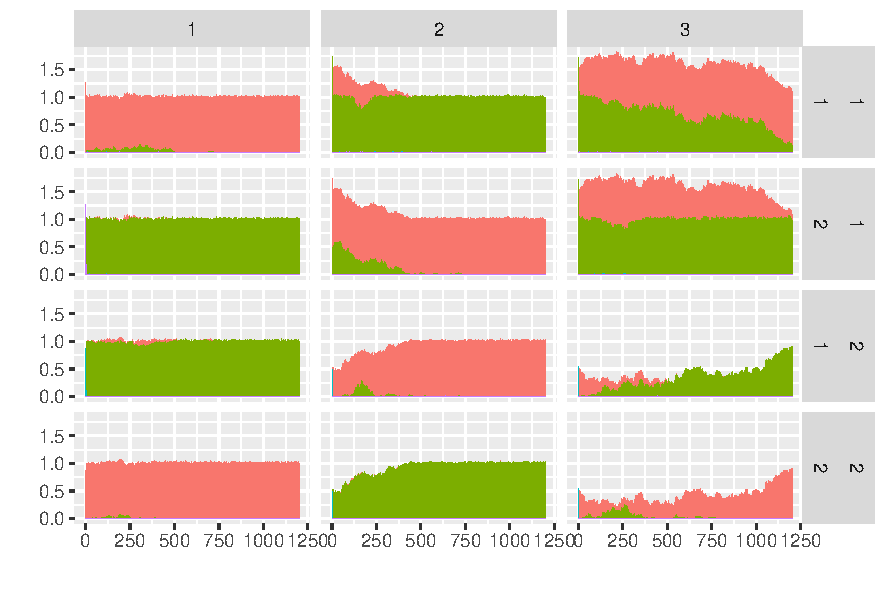
\includegraphics[scale=1]{plotalpha.pdf}}


\end{minipage}\hspace{.74cm}%
    }
    
    
    
    
    }
%%%%%%%%%%%%%%%%%%%%%%%%%%%%%%%%%%%%%%%%%%%%%%%%%%%
\def\blockref{

    \block{References}{
\small{
Dau, H. D., \& Chopin, N. (2022). Waste-free sequential monte carlo. Journal of the Royal Statistical Society Series B: Statistical Methodology, 84(1), 114-148.

Quince, C., Delmont, T. O., Raguideau, S., Alneberg, J., Darling, A. E., Collins, G., \& Eren, A. M. (2017). DESMAN: a new tool for de novo extraction of strains from metagenomes. Genome biology, 18, 1-22.
}}}
%%%%%%%%%%%%%%%%%%%%%%%%%%%%%%%%%%%%%%%%%%%%%%%%%%%



\begin{document}

%\maketitle[titletotopverticalspace=12cm]
\makeatletter
    \setlength{\TP@blocktop}{.48\textheight}
\makeatother

%\begin{columns}
%    \column{0.2}
%\useblockstyle{instituteblock} 
%\block{}{\color{color1}\normalsize\underline{Équipe de recherche}\\
%¹ Université Paris-Saclay, INRAE, MaIAGE, Jouy-en-Josas, France\\
%² Ensae, Palaiseau, France\\
%³ Crest,
%⁴ Ensae}
%    \column{0.8}
\begin{columns}
\useblockstyle{titleblock} 
\column{0.15}
\block{}{\vspace*{-4cm}






\definecolor{c000091}{RGB}{0,0,145}
\definecolor{ce1000f}{RGB}{225,0,15}
\definecolor{grey}{RGB}{128,128,128}


\def \globalscale {1.000000}
\begin{tikzpicture}[y=.05cm, x=.05cm, yscale=\globalscale,xscale=\globalscale, every node/.append style={scale=\globalscale}, inner sep=0pt, outer sep=0pt]
  \path[fill=white] (0.0, 0.0) -- (224.8958, 0.0) -- (224.8958, -202.9354) -- (0.0, -202.9354) -- cycle;



  \path[fill=c000091] (56.7531, -49.8475).. controls (57.0442, -49.5565) and (57.3352, -49.2654) .. (57.5998, -48.9479).. controls (58.129, -48.3394) and (58.6581, -47.7838) .. (59.2667, -47.2546).. controls (59.4519, -47.0958) and (59.6371, -46.9371) .. (59.8223, -46.8313).. controls (59.8752, -46.7783) and (59.8752, -46.6725) .. (59.9281, -46.6196).. controls (59.69, -46.7254) and (59.5313, -46.9106) .. (59.2667, -47.0165).. controls (59.2138, -47.0165) and (59.1608, -46.9635) .. (59.2138, -46.9106).. controls (59.399, -46.7783) and (59.5842, -46.646) .. (59.7429, -46.5138) -- (59.7165, -46.5138).. controls (59.6635, -46.5138) and (59.6635, -46.4608) .. (59.6635, -46.4079).. controls (59.0021, -46.3021) and (58.5258, -46.7519) .. (58.076, -47.1488).. controls (57.9702, -47.2017) and (57.8644, -47.0958) .. (57.8379, -47.0958).. controls (57.0971, -47.334) and (56.5415, -47.9954) .. (55.8006, -48.2865) -- (55.8006, -48.1806).. controls (55.5096, -48.2865) and (55.2185, -48.4717) .. (54.901, -48.5246).. controls (54.4513, -48.6304) and (54.0544, -48.5775) .. (53.6575, -48.5775).. controls (53.049, -48.6304) and (52.4404, -48.7627) .. (51.8319, -48.895).. controls (51.8054, -48.895) and (51.8054, -48.895) .. (51.779, -48.9215).. controls (51.4615, -49.0008) and (51.144, -49.1331) .. (50.8529, -49.2919) -- (50.7471, -49.3977).. controls (50.6413, -49.5035) and (50.5354, -49.6358) .. (50.4031, -49.6888).. controls (50.0856, -49.8475) and (49.8475, -50.1121) .. (49.5829, -50.3502).. controls (49.5565, -50.3767) and (49.53, -50.3767) .. (49.5035, -50.3767).. controls (49.239, -50.6413) and (48.9744, -50.9058) .. (48.7098, -51.144).. controls (48.6833, -51.1704) and (48.604, -51.1704) .. (48.551, -51.1704).. controls (48.551, -51.144) and (48.5775, -51.144) .. (48.5775, -51.1175).. controls (48.6304, -51.0381) and (48.6569, -50.9852) .. (48.7098, -50.9058) -- (48.8685, -50.6677).. controls (48.9479, -50.5619) and (49.0008, -50.456) .. (49.0802, -50.3767).. controls (49.1067, -50.3502) and (49.1067, -50.3238) .. (49.0802, -50.3238).. controls (49.0538, -50.2973) and (49.0273, -50.2973) .. (49.0008, -50.2973).. controls (49.239, -50.0592) and (49.5565, -49.8475) .. (49.8475, -49.6623).. controls (49.821, -49.6623) and (49.7681, -49.6358) .. (49.7946, -49.6094).. controls (49.821, -49.5565) and (49.8475, -49.53) .. (49.874, -49.4771).. controls (49.874, -49.4506) and (49.874, -49.4506) .. (49.9004, -49.4242).. controls (49.9004, -49.3977) and (49.874, -49.3977) .. (49.874, -49.3713) -- (49.6358, -49.53).. controls (49.5035, -49.6358) and (49.4242, -49.8475) .. (49.239, -49.8475) -- (49.1596, -49.8475).. controls (49.1331, -49.8475) and (49.1067, -49.8475) .. (49.1067, -49.821) -- (49.1067, -49.7946).. controls (49.1067, -49.7681) and (49.1331, -49.7681) .. (49.1331, -49.7417).. controls (49.1596, -49.6888) and (49.1596, -49.6623) .. (49.186, -49.6623).. controls (49.186, -49.6358) and (49.2125, -49.6094) .. (49.2125, -49.6094).. controls (49.2125, -49.5829) and (49.239, -49.5829) .. (49.239, -49.5565).. controls (49.2654, -49.53) and (49.2919, -49.4771) .. (49.2919, -49.4506).. controls (49.2919, -49.4242) and (49.3183, -49.4242) .. (49.3183, -49.3977).. controls (49.3448, -49.3713) and (49.3448, -49.3448) .. (49.3713, -49.3183).. controls (49.3977, -49.2654) and (49.3713, -49.239) .. (49.3448, -49.239).. controls (49.4242, -49.1067) and (49.5565, -49.0273) .. (49.6888, -48.9479) -- (49.6623, -48.9479).. controls (49.8475, -48.8421) and (50.0592, -48.7363) .. (50.2444, -48.6304) -- (50.3238, -48.551).. controls (50.0327, -48.6569) and (49.7946, -48.7892) .. (49.53, -48.9479).. controls (49.53, -48.9479) and (49.4771, -48.9744) .. (49.4506, -49.0008).. controls (49.4506, -49.0008) and (49.3977, -49.0273) .. (49.3183, -48.9479) -- (49.3183, -48.9215).. controls (49.3713, -48.8156) and (49.53, -48.7627) .. (49.6094, -48.6833).. controls (49.6623, -48.6833) and (49.7152, -48.6833) .. (49.7152, -48.7363).. controls (51.3292, -47.4927) and (53.5252, -47.7838) .. (55.3773, -47.1488).. controls (55.536, -47.0429) and (55.6683, -46.9371) .. (55.8271, -46.8577).. controls (56.0652, -46.7519) and (56.2769, -46.5138) .. (56.5679, -46.355).. controls (56.9648, -46.064) and (57.2558, -45.6935) .. (57.4146, -45.2173).. controls (57.4146, -45.1644) and (57.3617, -45.1115) .. (57.3617, -45.1115).. controls (56.7002, -45.7994) and (55.9594, -46.355) .. (55.1656, -46.7519).. controls (54.1073, -47.3075) and (52.9696, -47.2017) .. (51.8583, -47.3604).. controls (51.9113, -47.2546) and (52.0171, -47.2546) .. (52.0965, -47.2546).. controls (52.0965, -47.0958) and (52.2023, -47.0429) .. (52.3081, -46.9635) -- (52.4669, -46.9635).. controls (52.5198, -46.9635) and (52.5198, -46.8577) .. (52.5727, -46.8577).. controls (52.6785, -46.8577) and (52.8373, -46.8048) .. (52.7844, -46.8048).. controls (52.6256, -46.5931) and (52.3346, -46.9635) .. (52.0965, -46.8048).. controls (52.2023, -46.699) and (52.1494, -46.5667) .. (52.2552, -46.5138) -- (52.4669, -46.5138).. controls (52.4669, -46.4079) and (52.5727, -46.3021) .. (52.5727, -46.3021).. controls (53.3135, -45.8523) and (54.0279, -45.5083) .. (54.7158, -45.1115).. controls (54.5571, -45.1115) and (54.4777, -45.2702) .. (54.319, -45.1644).. controls (54.4248, -45.1644) and (54.319, -45.0056) .. (54.4248, -45.0056).. controls (54.9804, -44.8469) and (55.4302, -44.5558) .. (55.9858, -44.3442).. controls (55.7742, -44.3442) and (55.6419, -44.5029) .. (55.4302, -44.3442).. controls (55.536, -44.2913) and (55.589, -44.1854) .. (55.7213, -44.1854) -- (55.7213, -44.0267).. controls (55.7213, -43.9738) and (55.7742, -43.9738) .. (55.8271, -43.9738).. controls (55.7742, -43.9738) and (55.7213, -43.9208) .. (55.7213, -43.9208).. controls (55.7742, -43.815) and (55.9329, -43.8679) .. (56.0123, -43.7621).. controls (55.9594, -43.7621) and (55.8535, -43.7621) .. (55.8535, -43.7092).. controls (56.0123, -43.4975) and (56.2504, -43.471) .. (56.515, -43.4181).. controls (56.4621, -43.3123) and (56.3033, -43.4181) .. (56.3033, -43.3123).. controls (56.3033, -43.2594) and (56.3563, -43.2594) .. (56.4092, -43.2594) -- (56.3033, -43.2594).. controls (56.1975, -43.2065) and (56.2504, -43.1006) .. (56.2504, -43.0477).. controls (56.5415, -42.7038) and (56.5415, -42.254) .. (56.7002, -41.8571).. controls (56.6473, -41.8571) and (56.5944, -41.8571) .. (56.5944, -41.8042).. controls (56.0917, -42.3598) and (55.2979, -42.545) .. (54.5571, -42.7567) -- (54.2131, -42.7567).. controls (53.975, -42.8625) and (53.6046, -42.8625) .. (53.3665, -42.7038).. controls (53.1548, -42.5979) and (53.0754, -42.4656) .. (52.8638, -42.3069).. controls (52.4669, -42.0688) and (52.07, -41.8571) .. (51.6202, -41.6983).. controls (50.3767, -41.3015) and (49.0802, -41.0898) .. (47.7838, -41.1427).. controls (48.3394, -40.8517) and (48.9479, -40.8252) .. (49.53, -40.64).. controls (50.3767, -40.4019) and (51.1704, -40.0844) .. (52.07, -40.1373).. controls (51.9113, -40.0844) and (51.726, -40.1373) .. (51.5673, -40.1373).. controls (50.8794, -40.0844) and (50.165, -40.296) .. (49.4242, -40.4283).. controls (48.9215, -40.5342) and (48.4717, -40.7194) .. (47.969, -40.8252).. controls (47.6779, -40.931) and (47.5192, -41.2221) .. (47.1752, -41.1692) -- (47.1752, -41.0104).. controls (47.6779, -40.4019) and (48.2865, -39.8198) .. (49.0802, -39.7669).. controls (49.9798, -39.6081) and (50.8265, -39.7669) .. (51.726, -39.8727).. controls (52.3875, -39.9256) and (52.9696, -40.0844) .. (53.631, -40.2167).. controls (53.8692, -40.2167) and (53.9221, -40.6135) .. (54.1338, -40.6665).. controls (54.4248, -40.7723) and (54.7423, -40.6665) .. (55.0333, -40.8781).. controls (55.0333, -40.7723) and (54.9804, -40.6665) .. (55.0333, -40.5871).. controls (55.245, -40.3754) and (55.4831, -40.64) .. (55.6948, -40.5342).. controls (56.0917, -40.296) and (55.3508, -39.8463) .. (55.1392, -39.4758).. controls (55.1392, -39.4229) and (55.1921, -39.37) .. (55.1921, -39.37).. controls (55.589, -39.714) and (55.88, -40.1108) .. (56.3827, -40.3754).. controls (56.6208, -40.4813) and (57.2294, -40.6135) .. (57.1235, -40.3225).. controls (56.8854, -39.7669) and (56.3827, -39.3171) .. (55.9594, -38.8144) -- (55.9594, -38.6027).. controls (55.8535, -38.6027) and (55.8535, -38.5498) .. (55.8006, -38.4969) -- (55.8006, -38.2852).. controls (55.589, -38.1794) and (55.6419, -37.9942) .. (55.5625, -37.8354).. controls (55.4038, -37.5973) and (55.5096, -37.2269) .. (55.4038, -36.9358).. controls (55.2979, -36.6448) and (55.245, -36.3802) .. (55.1921, -36.0892).. controls (55.0333, -35.2425) and (54.8481, -34.5017) .. (54.7423, -33.6815).. controls (54.6365, -32.729) and (55.2979, -31.9881) .. (55.7477, -31.1415).. controls (56.0917, -30.5329) and (56.4885, -29.9508) .. (57.15, -29.554).. controls (57.3088, -28.9454) and (57.7056, -28.4427) .. (58.1025, -27.9665).. controls (58.4994, -27.4902) and (59.1608, -27.1727) .. (59.6371, -26.961).. controls (60.325, -26.6435) and (60.96, -26.4583) .. (60.96, -26.4583) -- (26.4583, -26.4583) -- (26.4583, -52.9167) -- (50.9852, -52.9167).. controls (51.9377, -52.2288) and (52.8902, -51.9113) .. (54.2131, -51.2498).. controls (54.8481, -50.9852) and (56.2769, -50.3238) .. (56.7531, -49.8475)(49.0802, -46.2492).. controls (48.9744, -46.2492) and (48.7892, -46.3021) .. (48.8421, -46.1963).. controls (48.895, -45.9581) and (49.239, -45.9581) .. (49.4506, -45.8523).. controls (49.5565, -45.7994) and (49.6888, -45.6935) .. (49.7946, -45.7465).. controls (49.9004, -45.9052) and (50.0327, -45.8523) .. (50.1385, -45.9581).. controls (49.821, -46.2492) and (49.4242, -46.1169) .. (49.0802, -46.2492)(41.4073, -45.1644).. controls (42.0158, -44.2119) and (42.4921, -43.4181) .. (42.9683, -42.5185).. controls (43.6298, -42.1746) and (44.159, -41.6719) .. (44.6617, -41.1163).. controls (45.5083, -40.2167) and (46.4079, -39.4229) .. (47.4663, -38.9202).. controls (47.8631, -38.7615) and (48.3658, -38.8144) .. (48.7627, -38.9731).. controls (48.604, -39.1848) and (48.3658, -39.1319) .. (48.1542, -39.2642).. controls (48.1013, -39.2642) and (48.0483, -39.2642) .. (47.9954, -39.2113).. controls (48.0483, -39.1583) and (48.0483, -39.1054) .. (48.0483, -39.0525).. controls (47.5456, -39.6081) and (46.8577, -39.8463) .. (46.4608, -40.5077).. controls (46.1698, -41.0104) and (45.9581, -41.6454) .. (45.3231, -41.8042).. controls (45.1115, -41.8571) and (45.376, -41.6454) .. (45.2702, -41.6983).. controls (43.7092, -42.6508) and (42.6244, -43.815) .. (41.4073, -45.1644)(45.5613, -41.8571).. controls (45.5083, -41.9629) and (45.4554, -41.9629) .. (45.4025, -42.0688).. controls (45.3496, -42.1746) and (45.2967, -42.2275) .. (45.1908, -42.2804).. controls (45.1379, -42.2804) and (45.085, -42.2804) .. (45.085, -42.2275).. controls (45.1379, -42.0158) and (45.2967, -41.8306) .. (45.4819, -41.7777).. controls (45.5613, -41.7513) and (45.5613, -41.8042) .. (45.5613, -41.8571)(47.8896, -49.3448).. controls (47.8631, -49.3977) and (47.8102, -49.4506) .. (47.7573, -49.5035).. controls (47.8102, -49.5035) and (47.8631, -49.5565) .. (47.8102, -49.5829).. controls (47.7044, -49.6888) and (47.5721, -49.7946) .. (47.4398, -49.8475) -- (47.3604, -49.8475).. controls (47.3075, -49.9004) and (47.2281, -49.9533) .. (47.1752, -50.0327).. controls (47.1223, -50.0856) and (46.8313, -50.0592) .. (46.9106, -49.9798).. controls (47.0429, -49.874) and (47.1488, -49.7417) .. (47.281, -49.6358).. controls (47.3604, -49.5829) and (47.4398, -49.5035) .. (47.4927, -49.4242).. controls (47.5192, -49.3713) and (47.5456, -49.3448) .. (47.5985, -49.3183).. controls (47.6779, -49.2654) and (47.9425, -49.239) .. (47.8896, -49.3448)(46.99, -48.9479).. controls (46.7783, -49.0802) and (46.5931, -49.2125) .. (46.4079, -49.3448).. controls (46.1963, -49.4771) and (45.9581, -49.5565) .. (45.7465, -49.6623).. controls (45.72, -49.6358) and (45.6935, -49.6358) .. (45.6671, -49.6358).. controls (45.4819, -49.7417) and (45.3231, -49.874) .. (45.1644, -50.0327) -- (45.085, -50.1121) -- (45.0056, -50.1915) -- (44.8998, -50.2973).. controls (44.8733, -50.3238) and (44.8733, -50.3502) .. (44.8204, -50.3767).. controls (44.794, -50.4031) and (44.7146, -50.4031) .. (44.7146, -50.3502).. controls (44.6881, -50.3767) and (44.6617, -50.3767) .. (44.6352, -50.4031).. controls (44.6088, -50.4296) and (44.5823, -50.4296) .. (44.5558, -50.456) -- (44.5029, -50.456).. controls (44.45, -50.509) and (44.3706, -50.5619) .. (44.3177, -50.6148).. controls (44.2119, -50.7206) and (44.106, -50.8) .. (44.0267, -50.9323) -- (44.0267, -50.9588) -- (44.0002, -50.9852).. controls (43.9738, -51.0381) and (43.9473, -51.0381) .. (43.9473, -51.0646).. controls (43.9473, -51.0646) and (43.9208, -51.091) .. (43.8944, -51.091) -- (43.8679, -51.0646).. controls (43.815, -51.0117) and (43.815, -50.9852) .. (43.7885, -50.9588) -- (43.7885, -50.9323).. controls (43.8415, -50.8794) and (43.8944, -50.8265) .. (43.9473, -50.7471).. controls (43.9738, -50.7206) and (43.9738, -50.6942) .. (44.0002, -50.6942).. controls (44.0267, -50.6677) and (44.0531, -50.6148) .. (44.0796, -50.5883).. controls (44.0796, -50.5619) and (44.106, -50.5619) .. (44.106, -50.5354).. controls (44.159, -50.456) and (44.2119, -50.4031) .. (44.2648, -50.3238) -- (44.2913, -50.2973).. controls (44.3177, -50.2708) and (44.3442, -50.2179) .. (44.3706, -50.1915) -- (44.4235, -50.0592).. controls (44.45, -50.0063) and (44.45, -49.9798) .. (44.4765, -49.9533) -- (44.4765, -49.9269).. controls (44.4765, -49.9004) and (44.4765, -49.9004) .. (44.5029, -49.874).. controls (44.5029, -49.8475) and (44.5029, -49.821) .. (44.5294, -49.7946) -- (44.5294, -49.7681).. controls (44.5823, -49.6623) and (44.6617, -49.5829) .. (44.741, -49.5035) -- (44.7146, -49.5035).. controls (44.6352, -49.5565) and (44.5823, -49.6094) .. (44.5294, -49.6623).. controls (44.4765, -49.7152) and (44.3706, -49.6358) .. (44.45, -49.5829).. controls (44.5029, -49.5565) and (44.5294, -49.5035) .. (44.5558, -49.4771).. controls (44.6352, -49.3977) and (44.7146, -49.2919) .. (44.8204, -49.2125).. controls (44.8733, -49.1596) and (44.9263, -49.1331) .. (44.9792, -49.1067) -- (45.0056, -49.0802).. controls (45.0321, -49.0273) and (45.085, -49.0008) .. (45.1115, -48.9479).. controls (45.5877, -48.4981) and (46.4079, -48.4981) .. (47.0165, -48.2071).. controls (47.2546, -48.1013) and (47.5721, -48.26) .. (47.8102, -48.2071).. controls (47.969, -48.2071) and (48.1013, -48.2071) .. (48.26, -48.3129).. controls (47.8102, -48.3923) and (47.4133, -48.6833) .. (46.99, -48.9479)(48.0219, -45.4554).. controls (47.969, -45.4025) and (48.1806, -45.4554) .. (48.2335, -45.3496) -- (47.8367, -45.3496).. controls (47.7838, -45.3496) and (47.7838, -45.2967) .. (47.7838, -45.2438).. controls (47.5456, -45.2967) and (47.2281, -45.4025) .. (46.99, -45.4554).. controls (46.646, -45.5613) and (46.3285, -45.7994) .. (45.9317, -45.9052).. controls (45.376, -46.1169) and (44.9263, -46.5667) .. (44.3442, -46.7519).. controls (44.2913, -46.7519) and (44.2913, -46.699) .. (44.2913, -46.646).. controls (44.3442, -46.4873) and (44.5294, -46.4344) .. (44.6352, -46.3021).. controls (44.6352, -46.2492) and (44.6352, -46.1963) .. (44.5823, -46.1963).. controls (44.9792, -45.6406) and (45.5348, -45.3496) .. (46.0375, -44.8998) -- (46.0375, -44.741).. controls (46.1963, -44.5294) and (46.4344, -44.45) .. (46.5402, -44.1854).. controls (46.5931, -44.0267) and (46.8048, -43.8415) .. (47.0429, -43.7356).. controls (46.99, -43.6827) and (46.8842, -43.6827) .. (46.8842, -43.5769).. controls (46.6725, -43.5769) and (46.4873, -43.6827) .. (46.2756, -43.524).. controls (46.3815, -43.4446) and (46.4873, -43.3917) .. (46.5931, -43.3388).. controls (46.5402, -43.3388) and (46.5138, -43.3123) .. (46.4873, -43.2594).. controls (46.4344, -43.1535) and (46.5931, -43.0477) .. (46.7254, -43.0213).. controls (46.9371, -42.9683) and (47.1752, -42.9683) .. (47.334, -42.8096).. controls (46.99, -42.7567) and (46.5931, -42.9154) .. (46.2227, -42.7038).. controls (46.4608, -42.0423) and (46.8842, -41.5131) .. (47.4663, -41.1956).. controls (47.5192, -41.1956) and (47.625, -41.1956) .. (47.625, -41.2485).. controls (47.625, -41.4867) and (47.4663, -41.6983) .. (47.2281, -41.7513).. controls (47.625, -41.8571) and (48.0219, -41.8571) .. (48.4188, -42.0423).. controls (48.3658, -42.1481) and (48.26, -42.0952) .. (48.2071, -42.0952).. controls (48.4452, -42.254) and (48.7627, -42.1481) .. (49.0008, -42.3333).. controls (48.8421, -42.4921) and (48.7098, -42.3333) .. (48.551, -42.3333).. controls (50.1121, -42.7831) and (51.7525, -43.1271) .. (53.049, -44.1325).. controls (51.9377, -44.6881) and (50.8, -44.9263) .. (49.6094, -45.1908).. controls (49.4506, -45.1908) and (49.3713, -45.1908) .. (49.2125, -45.1379).. controls (49.2125, -45.1908) and (49.2125, -45.2967) .. (49.1596, -45.2967).. controls (48.9479, -45.2967) and (48.8156, -45.2967) .. (48.6569, -45.4025).. controls (48.4717, -45.5613) and (48.1806, -45.6142) .. (48.0219, -45.4554);



  \path[fill=ce1000f] (99.351, -26.4583) -- (70.9348, -26.4583).. controls (71.4375, -26.7229) and (71.7285, -26.8817) .. (71.9138, -26.961).. controls (72.2842, -27.1463) and (72.6281, -27.3844) .. (72.8663, -27.7548).. controls (72.9721, -27.9135) and (73.1044, -28.2046) .. (73.025, -28.4163).. controls (72.9192, -28.6544) and (72.8663, -29.0777) .. (72.6281, -29.1571).. controls (72.3371, -29.3158) and (71.9402, -29.3158) .. (71.5698, -29.2629).. controls (71.3581, -29.2629) and (71.1729, -29.21) .. (70.9613, -29.1571).. controls (71.7021, -29.4481) and (72.4165, -29.8185) .. (72.9192, -30.5065).. controls (72.9721, -30.6123) and (73.1573, -30.6652) .. (73.369, -30.6652).. controls (73.4219, -30.6652) and (73.4219, -30.771) .. (73.4219, -30.824).. controls (73.316, -30.9298) and (73.2102, -30.9827) .. (73.2631, -31.115) -- (73.4219, -31.115).. controls (73.66, -31.0092) and (73.6335, -30.5065) .. (73.9775, -30.6652).. controls (74.2156, -30.824) and (74.3215, -31.1679) .. (74.1892, -31.406).. controls (73.9775, -31.6177) and (73.7923, -31.75) .. (73.5806, -31.9088).. controls (73.5277, -32.0146) and (73.5277, -32.1469) .. (73.5806, -32.2527).. controls (73.7394, -32.4644) and (73.7923, -32.6496) .. (73.8188, -32.8613).. controls (73.9775, -33.2052) and (74.0304, -33.6021) .. (74.1627, -33.9725).. controls (74.3744, -34.7133) and (74.5596, -35.4806) .. (74.5067, -36.2215).. controls (74.5067, -36.6183) and (74.295, -36.9623) .. (74.4537, -37.3592).. controls (74.5596, -37.756) and (74.7977, -38.0471) .. (75.0094, -38.4175).. controls (75.221, -38.7085) and (75.4062, -38.9202) .. (75.565, -39.2113).. controls (75.856, -39.714) and (76.4117, -40.2167) .. (76.1735, -40.7988).. controls (76.0148, -41.1427) and (75.4856, -41.0898) .. (75.1152, -41.3015).. controls (74.8242, -41.5396) and (75.0623, -41.9629) .. (75.221, -42.201).. controls (75.4592, -42.6508) and (74.93, -42.9419) .. (74.5596, -43.0742).. controls (74.6654, -43.2329) and (74.8506, -43.18) .. (74.9035, -43.2858).. controls (74.9565, -43.524) and (75.1946, -43.6827) .. (75.0623, -43.9473).. controls (74.8506, -44.2383) and (74.2685, -44.3971) .. (74.5596, -44.8469).. controls (74.7713, -45.1908) and (74.639, -45.5877) .. (74.5067, -45.9581).. controls (74.3479, -46.355) and (74.004, -46.6196) .. (73.6071, -46.699).. controls (73.316, -46.8048) and (72.9456, -46.8048) .. (72.6546, -46.7519).. controls (72.5488, -46.699) and (72.4429, -46.646) .. (72.3635, -46.646).. controls (71.5169, -46.5402) and (70.6702, -46.3021) .. (69.8235, -46.3021).. controls (69.5854, -46.355) and (69.3208, -46.4079) .. (69.1356, -46.4873).. controls (68.924, -46.646) and (68.7123, -46.8313) .. (68.5271, -47.0165).. controls (68.5006, -47.0694) and (68.4477, -47.0958) .. (68.4213, -47.1488).. controls (68.3948, -47.1752) and (68.3683, -47.2017) .. (68.3683, -47.2281) -- (68.3154, -47.281).. controls (68.1567, -47.4663) and (68.0508, -47.6515) .. (67.9185, -47.8631).. controls (67.9185, -47.8896) and (67.8921, -47.8896) .. (67.8921, -47.8896).. controls (67.8921, -47.916) and (67.8656, -47.9425) .. (67.8392, -47.969).. controls (67.6804, -48.26) and (67.5481, -48.5775) .. (67.4688, -48.895).. controls (67.1248, -50.0327) and (67.2835, -51.0117) .. (67.5217, -51.2498).. controls (67.5746, -51.3027) and (69.1621, -51.8054) .. (70.2733, -52.3081).. controls (70.8025, -52.5463) and (71.1465, -52.705) .. (71.464, -52.9167) -- (99.3775, -52.9167) -- (99.3775, -26.4583) -- cycle;



  \path[fill=grey] (72.6281, -36.1421).. controls (72.8398, -36.195) and (73.1308, -36.195) .. (73.1308, -36.3008).. controls (73.025, -36.6977) and (72.4429, -36.8035) .. (72.1254, -37.2004) -- (71.9667, -37.2004).. controls (71.8079, -37.3063) and (71.8608, -37.5444) .. (71.7285, -37.5444).. controls (71.5698, -37.4915) and (71.4375, -37.5444) .. (71.2788, -37.5973).. controls (71.4904, -37.809) and (71.7285, -37.9413) .. (72.0196, -37.8883).. controls (72.0725, -37.8883) and (72.1783, -37.9942) .. (72.1783, -38.1).. controls (72.1783, -38.1) and (72.2313, -38.1) .. (72.2842, -38.0471).. controls (72.3371, -38.0471) and (72.39, -38.0471) .. (72.39, -38.1) -- (72.39, -38.3117).. controls (72.2313, -38.5233) and (71.9931, -38.4175) .. (71.7815, -38.4704).. controls (72.1783, -38.5763) and (72.5752, -38.5763) .. (72.9456, -38.4704).. controls (73.2367, -38.3646) and (72.9456, -37.8619) .. (73.1573, -37.6238).. controls (73.0515, -37.6238) and (73.1573, -37.465) .. (73.0515, -37.465).. controls (73.1573, -37.3592) and (73.2631, -37.2269) .. (73.3425, -37.174).. controls (73.4483, -37.174) and (73.5806, -37.121) .. (73.6335, -37.0152).. controls (73.6335, -36.9094) and (73.4219, -36.8565) .. (73.4748, -36.7771).. controls (73.7658, -36.5654) and (74.0304, -36.2744) .. (73.9246, -35.9833).. controls (73.8717, -35.8246) and (73.4748, -35.8246) .. (73.2367, -35.7188).. controls (72.1519, -35.7717) and (71.8873, -35.9304) .. (71.6492, -35.9833).. controls (71.3052, -36.0892) and (70.9877, -36.2744) .. (70.6967, -36.486).. controls (71.0406, -36.3273) and (71.3846, -36.2744) .. (71.7815, -36.195).. controls (72.0725, -36.1421) and (72.3106, -36.0892) .. (72.6281, -36.1421);



  \path[fill] (26.4583, -85.9896) -- (26.4583, -66.1458) -- (32.4908, -66.1458) .. controls (34.6781, -66.1458) and (36.389, -66.675) .. (37.6238, -67.7333) .. controls (38.8761, -68.7917) and (39.5111, -70.2381) .. (39.5288, -72.0725) .. controls (39.5288, -73.2543) and (39.2553, -74.2774) .. (38.7085, -75.1417) .. controls (38.1617, -76.0236) and (37.3856, -76.7115) .. (36.3802, -77.2054) -- (42.5715, -85.9896) -- (37.7825, -85.9896) -- (32.5173, -77.9727) -- (30.48, -77.9727) -- (30.48, -85.9896) -- cycle(30.48, -74.5596) -- (32.729, -74.5596) .. controls (33.5756, -74.5596) and (34.2283, -74.3391) .. (34.6869, -73.8981) .. controls (35.1631, -73.4572) and (35.4013, -72.831) .. (35.4013, -72.0196) .. controls (35.4013, -71.2611) and (35.1631, -70.6614) .. (34.6869, -70.2204) .. controls (34.2106, -69.7794) and (33.558, -69.5678) .. (32.729, -69.5854) -- (30.48, -69.5854) -- cycle(45.376, -85.9896) -- (45.376, -66.1458) -- (56.8854, -66.1458) -- (56.8854, -69.5854) -- (49.3713, -69.5854) -- (49.3713, -74.1627) -- (55.7477, -74.1627) -- (55.7477, -77.6023) -- (49.3713, -77.6023) -- (49.3713, -82.55) -- (56.8854, -82.55) -- (56.8854, -85.9896) -- cycle(49.2654, -64.4525) -- (52.4404, -60.616) -- (56.5679, -60.616) -- (52.9167, -64.4525) -- cycle(61.7802, -85.9896) -- (61.7802, -66.1458) -- (68.3154, -66.1458) .. controls (70.485, -66.1458) and (72.1872, -66.675) .. (73.4219, -67.7333) .. controls (74.6742, -68.7917) and (75.3004, -70.2381) .. (75.3004, -72.0725) .. controls (75.3004, -73.9069) and (74.6742, -75.3445) .. (73.4219, -76.3852) .. controls (72.1695, -77.4435) and (70.4674, -77.9727) .. (68.3154, -77.9727) -- (65.8019, -77.9727) -- (65.8019, -85.9896) -- cycle(65.8019, -74.5596) -- (68.4742, -74.5596) .. controls (69.3385, -74.5596) and (70.0088, -74.3303) .. (70.485, -73.8717) .. controls (70.9613, -73.4307) and (71.1994, -72.8133) .. (71.1994, -72.0196) .. controls (71.1994, -71.2611) and (70.9524, -70.6614) .. (70.4585, -70.2204) .. controls (69.9823, -69.7794) and (69.3208, -69.5678) .. (68.4742, -69.5854) -- (65.8019, -69.5854) -- cycle(78.5283, -78.2373) -- (78.5283, -66.1458) -- (82.55, -66.1458) -- (82.55, -78.5548) .. controls (82.55, -79.8777) and (82.9028, -80.9184) .. (83.6083, -81.6769) .. controls (84.3139, -82.4177) and (85.2928, -82.7881) .. (86.5452, -82.7881) .. controls (87.7799, -82.7881) and (88.7501, -82.4177) .. (89.4556, -81.6769) .. controls (90.1612, -80.936) and (90.514, -79.8953) .. (90.514, -78.5548) -- (90.514, -66.1458) -- (94.5356, -66.1458) -- (94.5356, -78.2373) .. controls (94.5356, -80.8478) and (93.8213, -82.8851) .. (92.3925, -84.3492) .. controls (84.0493, -86.5452) and (82.1002, -85.8132) .. (80.6715, -84.3492) .. controls (79.2427, -82.8675) and (78.5283, -80.8302) .. (78.5283, -78.2373) -- cycle(99.7744, -85.9896) -- (99.7744, -66.1458) -- (105.3835, -66.1458) .. controls (107.4473, -66.1458) and (109.0613, -66.6221) .. (110.2254, -67.5746) .. controls (111.4072, -68.5271) and (111.9981, -69.85) .. (111.9981, -71.5433) .. controls (111.9981, -73.1838) and (111.3014, -74.489) .. (109.9079, -75.4592) .. controls (110.9486, -75.9354) and (111.7512, -76.5704) .. (112.3156, -77.3642) .. controls (112.8801, -78.1756) and (113.1623, -79.1016) .. (113.1623, -80.1423) .. controls (113.1623, -81.9591) and (112.5008, -83.3878) .. (111.1779, -84.4285) .. controls (109.8726, -85.4692) and (108.0823, -85.9896) .. (105.8069, -85.9896) -- cycle(103.7696, -82.55) -- (106.045, -82.55) .. controls (106.9799, -82.55) and (107.7119, -82.3207) .. (108.241, -81.8621) .. controls (108.7702, -81.3858) and (109.0348, -80.742) .. (109.0348, -79.9306) .. controls (109.0348, -79.1192) and (108.7702, -78.4842) .. (108.241, -78.0256) .. controls (107.7119, -77.5847) and (106.9799, -77.3642) .. (106.045, -77.3642) -- (103.7696, -77.3642) -- cycle(103.7696, -73.9246) -- (105.4629, -73.9246) .. controls (106.2214, -73.9246) and (106.8123, -73.7306) .. (107.2356, -73.3425) .. controls (107.659, -72.9721) and (107.8706, -72.4341) .. (107.8706, -71.7285) .. controls (107.8706, -71.0583) and (107.659, -70.5379) .. (107.2356, -70.1675) .. controls (106.8299, -69.7794) and (106.239, -69.5854) .. (105.4629, -69.5854) -- (103.7696, -69.5854) -- cycle(117.5279, -85.9896) -- (117.5279, -66.1458) -- (121.5231, -66.1458) -- (121.5231, -82.3383) -- (129.0373, -82.3383) -- (129.0373, -85.9896) -- cycle(132.8473, -85.9896) -- (132.8473, -66.1458) -- (136.8425, -66.1458) -- (136.8425, -85.9896) -- cycle(141.7373, -80.1158) .. controls (141.2258, -78.8282) and (140.97, -77.4788) .. (140.97, -76.0677) .. controls (142.2488, -70.7584) and (142.9544, -69.6383) .. (143.854, -68.6858) .. controls (144.7712, -67.7333) and (145.8824, -66.9749) .. (147.1877, -66.4104) .. controls (148.5106, -65.846) and (149.9306, -65.5637) .. (151.4475, -65.5637) .. controls (152.9644, -65.5637) and (154.3844, -65.846) .. (155.7073, -66.4104) .. controls (157.0302, -66.9749) and (158.1415, -67.7333) .. (159.041, -68.6858) .. controls (159.9406, -69.6383) and (160.6462, -70.7584) .. (161.1577, -72.046) .. controls (161.6692, -73.316) and (161.925, -74.6566) .. (161.925, -76.0677) .. controls (161.925, -77.7258) and (161.581, -79.278) .. (160.8931, -80.7244) -- (159.2263, -85.4869) .. controls (160.6197, -86.7569) and (161.9956, -87.3831) .. (163.3538, -87.3654) .. controls (163.9182, -87.3654) and (164.3944, -87.2949) .. (164.7825, -87.1538) -- (164.7825, -90.5669) .. controls (164.1651, -90.8138) and (163.4684, -90.9285) .. (162.6923, -90.9108) .. controls (160.558, -90.9108) and (158.5031, -90.0465) .. (156.5275, -88.3179) -- (154.1727, -86.2013) .. controls (153.3084, -86.4306) and (152.4, -86.5452) .. (151.4475, -86.5452) .. controls (149.9306, -86.5452) and (148.5106, -86.263) .. (147.1877, -85.6985) .. controls (145.8824, -85.1341) and (144.7712, -84.3844) .. (143.854, -83.4496) .. controls (142.9544, -82.4971) and (142.2488, -81.3858) .. (141.7373, -80.1158) -- cycle(146.8967, -71.2788) .. controls (145.6972, -72.5664) and (145.0887, -74.1627) .. (145.071, -76.0677) .. controls (145.071, -77.9727) and (145.6796, -79.569) .. (146.8967, -80.8567) .. controls (148.0961, -82.1443) and (149.6219, -82.7881) .. (151.474, -82.7881) .. controls (152.691, -82.7881) and (153.7758, -82.4971) .. (154.7283, -81.915) .. controls (155.6985, -81.3329) and (156.4569, -80.5215) .. (157.0038, -79.4808) .. controls (157.5506, -78.4578) and (157.824, -77.3201) .. (157.824, -76.0677) .. controls (157.824, -74.1627) and (157.2154, -72.5664) .. (155.9983, -71.2788) .. controls (154.7989, -69.9911) and (153.2819, -69.3473) .. (151.4475, -69.3473) .. controls (149.5954, -69.3473) and (148.0697, -69.9911) .. (146.8702, -71.2788) -- cycle(165.6821, -78.2373) -- (165.6821, -66.1458) -- (169.7038, -66.1458) -- (169.7038, -78.5548) .. controls (169.7038, -79.8777) and (170.0565, -80.9184) .. (170.7621, -81.6769) .. controls (171.4676, -82.4177) and (172.4466, -82.7881) .. (173.699, -82.7881) .. controls (174.9337, -82.7881) and (175.9038, -82.4177) .. (176.6094, -81.6769) .. controls (177.3149, -80.936) and (177.6677, -79.8953) .. (177.6677, -78.5548) -- (177.6677, -66.1458) -- (181.6894, -66.1458) -- (181.6894, -78.2373) .. controls (181.6894, -80.8478) and (180.975, -82.8851) .. (179.5463, -84.3492) .. controls (178.1175, -85.8308) and (176.1596, -86.5628) .. (173.6725, -86.5452) .. controls (171.2031, -86.5452) and (169.254, -85.8132) .. (167.8252, -84.3492) .. controls (166.3965, -82.8675) and (165.6821, -80.8302) .. (165.6821, -78.2373) -- cycle(186.9281, -85.9896) -- (186.9281, -66.1458) -- (198.4375, -66.1458) -- (198.4375, -69.5854) -- (190.9233, -69.5854) -- (190.9233, -74.1627) -- (197.2998, -74.1627) -- (197.2998, -77.6023) -- (190.9233, -77.6023) -- (190.9233, -82.55) -- (198.4375, -82.55) -- (198.4375, -85.9896) -- cycle(26.4583, -114.6969) -- (26.4583, -94.8531) -- (37.9677, -94.8531) -- (37.9677, -98.2927) -- (30.48, -98.2927) -- (30.48, -102.87) -- (36.8565, -102.87) -- (36.8565, -106.3096) -- (30.48, -106.3096) -- (30.48, -114.6969) -- cycle(41.7777, -114.6969) -- (41.7777, -94.8531) -- (47.8102, -94.8531) .. controls (49.9798, -94.8531) and (51.6996, -95.3823) .. (52.9696, -96.4406) .. controls (54.2219, -97.499) and (54.8481, -98.9453) .. (54.8481, -100.7798) .. controls (54.8481, -101.9616) and (54.5747, -102.9935) .. (54.0279, -103.8754) .. controls (53.4811, -104.7574) and (52.705, -105.4365) .. (51.6996, -105.9127) -- (57.8908, -114.6969) -- (53.1019, -114.6969) -- (47.8367, -106.68) -- (45.7994, -106.68) -- (45.7994, -114.6969) -- cycle(45.7994, -103.2669) -- (48.0483, -103.2669) .. controls (48.895, -103.2669) and (49.5565, -103.0464) .. (50.0327, -102.6054) .. controls (50.509, -102.1644) and (50.7383, -101.5383) .. (50.7206, -100.7269) .. controls (50.7206, -99.9684) and (50.4913, -99.3687) .. (50.0327, -98.9277) .. controls (49.5741, -98.4867) and (48.9126, -98.2751) .. (48.0483, -98.2927) -- (45.7994, -98.2927) -- cycle(59.0285, -114.6969) -- (66.5162, -94.8531) -- (71.755, -94.8531) -- (79.2427, -114.6969) -- (74.9829, -114.6969) -- (73.0779, -109.5375) -- (65.1669, -109.5375) -- (63.2883, -114.6969) -- cycle(66.4104, -106.0979) -- (71.8608, -106.0979) -- (69.1356, -98.6631) -- cycle(82.5765, -114.6969) -- (82.5765, -94.8531) -- (87.7094, -94.8531) -- (96.5465, -109.0613) -- (96.5465, -94.8531) -- (100.5417, -94.8531) -- (100.5417, -114.6969) -- (95.4088, -114.6969) -- (86.5717, -100.4358) -- (86.5717, -114.6969) -- cycle(104.6956, -104.775) .. controls (104.6956, -103.3639) and (104.9514, -102.0233) .. (105.4629, -100.7533) .. controls (105.9744, -99.4657) and (106.68, -98.3456) .. (107.5796, -97.3931) .. controls (108.4968, -96.4406) and (109.6081, -95.691) .. (110.9133, -95.1442) .. controls (112.2363, -94.5797) and (113.665, -94.2975) .. (115.1996, -94.2975) .. controls (116.9458, -94.2975) and (118.5333, -94.6503) .. (119.9621, -95.3558) .. controls (121.4085, -96.079) and (122.5903, -97.0668) .. (123.5075, -98.3192) -- (120.359, -100.7798) .. controls (119.7769, -99.9508) and (119.0449, -99.2893) .. (118.1629, -98.7954) .. controls (117.281, -98.3015) and (116.2932, -98.0546) .. (115.1996, -98.0546) .. controls (113.3475, -98.0546) and (111.8217, -98.6984) .. (110.6223, -99.986) .. controls (109.4228, -101.2737) and (108.8143, -102.87) .. (108.7967, -104.775) .. controls (108.7967, -106.68) and (109.4052, -108.2851) .. (110.6223, -109.5904) .. controls (111.8217, -110.8781) and (113.3475, -111.5131) .. (115.1996, -111.4954) .. controls (116.2932, -111.4954) and (117.281, -111.2573) .. (118.1629, -110.781) .. controls (119.0449, -110.2872) and (119.7769, -109.6169) .. (120.359, -108.7702) -- (123.5075, -111.2044) .. controls (122.7314, -112.2803) and (121.7613, -113.1623) .. (120.5971, -113.8502) .. controls (119.4329, -114.5381) and (118.1453, -114.9703) .. (116.7342, -115.1467) -- (114.2735, -119.2742) -- (110.7281, -119.2742) -- (113.2152, -115.0938) .. controls (111.5395, -114.7939) and (110.049, -114.1501) .. (108.7438, -113.1623) .. controls (107.4385, -112.1745) and (106.4331, -110.9486) .. (105.7275, -109.4846) .. controls (105.0219, -108.0206) and (104.678, -106.4507) .. (104.6956, -104.775) -- cycle(124.6717, -114.6969) -- (132.1594, -94.8531) -- (137.3981, -94.8531) -- (144.8858, -114.6969) -- (140.626, -114.6969) -- (138.7475, -109.5375) -- (130.8365, -109.5375) -- (128.9315, -114.6969) -- cycle(132.08, -106.0979) -- (137.504, -106.0979) -- (134.7788, -98.6631) -- cycle(148.2196, -114.6969) -- (148.2196, -94.8531) -- (152.2413, -94.8531) -- (152.2413, -114.6969) -- cycle(156.2629, -111.9452) -- (159.1733, -109.2729) .. controls (159.7731, -110.049) and (160.4433, -110.6488) .. (161.1842, -111.0721) .. controls (161.9426, -111.4954) and (162.7276, -111.7071) .. (163.539, -111.7071) .. controls (164.3327, -111.7071) and (164.9501, -111.5042) .. (165.391, -111.0985) .. controls (165.8497, -110.6928) and (166.079, -110.1284) .. (166.079, -109.4052) .. controls (166.079, -108.9819) and (165.9555, -108.5938) .. (165.7085, -108.241) .. controls (165.444, -107.8883) and (165.1, -107.5972) .. (164.6767, -107.3679) .. controls (164.2533, -107.121) and (163.7683, -106.874) .. (163.2215, -106.6271) .. controls (162.6747, -106.3625) and (162.119, -106.1067) .. (161.5546, -105.8598) .. controls (160.9901, -105.6128) and (160.4433, -105.313) .. (159.9142, -104.9602) .. controls (159.3674, -104.6074) and (158.8823, -104.2194) .. (158.459, -103.796) .. controls (158.0356, -103.3727) and (157.6917, -102.8347) .. (157.4271, -102.1821) .. controls (157.1625, -101.5294) and (157.0302, -100.8151) .. (157.0302, -100.039) .. controls (157.0302, -98.4338) and (157.6299, -97.0756) .. (158.8294, -95.9644) .. controls (160.0288, -94.8531) and (161.5458, -94.2975) .. (163.3802, -94.2975) .. controls (166.1319, -94.2975) and (168.4338, -95.4088) .. (170.2858, -97.6313) -- (167.349, -100.2771) .. controls (166.079, -98.619) and (164.7649, -97.79) .. (163.4067, -97.79) .. controls (162.7364, -97.79) and (162.1808, -97.9928) .. (161.7398, -98.3985) .. controls (161.1048, -100.2506) and (161.2106, -100.5946) .. (161.4223, -100.9121) .. controls (161.634, -101.2119) and (161.9074, -101.4853) .. (162.2425, -101.7323) .. controls (162.5953, -101.9616) and (163.001, -102.1909) .. (163.4596, -102.4202) -- (164.8619, -103.0817) .. controls (165.3734, -103.311) and (165.8761, -103.5403) .. (166.37, -103.7696) .. controls (166.8815, -104.0165) and (167.3578, -104.3164) .. (167.7988, -104.6692) .. controls (168.2574, -105.0043) and (168.6631, -105.3924) .. (169.0158, -105.8333) .. controls (169.3686, -106.2567) and (169.642, -106.7594) .. (169.836, -107.3415) .. controls (170.0477, -107.9412) and (170.1535, -108.6026) .. (170.1535, -109.3258) .. controls (170.1183, -111.125) and (169.4744, -112.5626) .. (168.2221, -113.6385) .. controls (166.9874, -114.7145) and (165.444, -115.2525) .. (163.5919, -115.2525) .. controls (161.9691, -115.2525) and (160.5668, -114.9791) .. (159.385, -114.4323) .. controls (158.2032, -113.8678) and (157.1625, -113.0388) .. (156.2629, -111.9452) -- cycle(174.625, -114.6969) -- (174.625, -94.8531) -- (186.1344, -94.8531) -- (186.1344, -98.2927) -- (178.6467, -98.2927) -- (178.6467, -102.87) -- (185.0231, -102.87) -- (185.0231, -106.3096) -- (178.6467, -106.3096) -- (178.6467, -111.2573) -- (186.1344, -111.2573) -- (186.1344, -114.6969) -- cycle;



  \path[fill] (92.1808, -169.0952).. controls (92.7629, -169.0952) and (93.2656, -169.545) .. (93.001, -170.5769) -- (90.3288, -171.2913).. controls (90.7521, -170.0213) and (91.5458, -169.0952) .. (92.1808, -169.0952)(93.6625, -173.4344) -- (93.1333, -173.4344).. controls (92.4719, -174.2281) and (91.731, -174.8631) .. (91.0167, -174.8631).. controls (90.2758, -174.8631) and (89.9054, -174.4133) .. (89.9054, -173.4344).. controls (89.9054, -173.0375) and (89.9583, -172.6142) .. (90.0377, -172.2438) -- (94.3769, -170.815).. controls (95.2235, -168.8042) and (94.1917, -167.931) .. (93.001, -167.931).. controls (90.9373, -167.931) and (88.609, -171.5294) .. (88.609, -174.3604).. controls (88.609, -175.7098) and (89.244, -176.4506) .. (90.2494, -176.4506).. controls (91.44, -176.4506) and (92.6571, -175.3129) .. (93.6625, -173.4344)(92.9746, -166.9785) -- (95.4352, -164.7296) -- (95.4352, -164.4121) -- (93.7948, -164.4121) -- (92.3396, -167.005) -- (92.9746, -167.005) -- cycle(83.7406, -169.1481) -- (85.1694, -169.1481) -- (82.894, -175.3923).. controls (82.6823, -175.9215) and (82.9733, -176.4506) .. (83.529, -176.4506).. controls (85.1429, -176.4506) and (87.0744, -175.0748) .. (87.8152, -173.1169) -- (87.4183, -173.1169).. controls (86.8363, -173.9371) and (85.5663, -174.8367) .. (84.6138, -175.0219) -- (86.704, -169.1481) -- (88.8471, -169.1481) -- (89.1117, -168.2485) -- (87.0215, -168.2485) -- (87.8152, -165.9996) -- (86.995, -165.9996) -- (85.5133, -168.2485) -- (83.7406, -168.4867) -- cycle(82.259, -168.8306).. controls (82.4442, -168.2485) and (82.0473, -167.931) .. (81.7563, -167.931).. controls (80.5127, -167.931) and (79.0046, -169.0688) .. (78.4225, -170.6298) -- (78.8194, -170.6298).. controls (79.2163, -170.0477) and (79.9042, -169.4127) .. (80.5656, -169.3069) -- (78.1579, -175.551).. controls (77.9463, -176.1331) and (78.3696, -176.4506) .. (78.6871, -176.4506).. controls (79.8777, -176.4506) and (81.28, -175.3129) .. (81.8621, -173.7519) -- (81.4652, -173.7519).. controls (81.0683, -174.334) and (80.3804, -174.969) .. (79.719, -175.0748) -- cycle(82.4971, -166.3435).. controls (83.0263, -166.3435) and (83.476, -165.8938) .. (83.476, -165.3646).. controls (82.2325, -164.3856) and (81.9944, -164.4915) .. (81.8092, -164.6767).. controls (81.624, -164.8619) and (81.5181, -165.1) .. (81.5181, -165.3646).. controls (81.5181, -165.9202) and (81.9415, -166.3435) .. (82.4971, -166.3435)(70.8819, -169.6773).. controls (71.2523, -169.6773) and (71.464, -170.2594) .. (70.8819, -171.5558) -- (69.1885, -175.3129).. controls (68.871, -176.0273) and (69.215, -176.4771) .. (69.9029, -176.4771).. controls (70.3263, -176.4771) and (70.5115, -176.3713) .. (70.6967, -175.9215) -- (72.3635, -171.5294).. controls (73.1308, -170.5769) and (74.5596, -169.5715) .. (75.1946, -169.5715).. controls (75.6444, -169.5715) and (75.5915, -169.9419) .. (75.3004, -170.524) -- (72.734, -175.4188).. controls (72.4958, -175.895) and (72.8133, -176.4771) .. (73.369, -176.4771).. controls (74.6125, -176.4771) and (76.1206, -175.3394) .. (76.7027, -173.7783) -- (76.2529, -173.7783).. controls (75.856, -174.3604) and (75.1681, -174.9954) .. (74.5067, -175.1013) -- (76.7027, -170.6563).. controls (76.9938, -170.1006) and (77.126, -169.5715) .. (77.126, -169.1481).. controls (77.126, -168.4338) and (76.7292, -167.9575) .. (75.9619, -167.9575).. controls (74.8771, -167.9575) and (73.951, -169.1746) .. (72.6281, -170.6827) -- (72.6281, -169.5185).. controls (72.6281, -168.6983) and (72.3635, -167.9575) .. (71.6227, -167.9575).. controls (70.7496, -167.9575) and (69.9558, -169.3333) .. (69.3208, -170.6563) -- (69.7177, -170.6563).. controls (70.1675, -170.0213) and (70.5644, -169.6773) .. (70.8819, -169.6773)(69.1621, -169.836).. controls (69.4531, -168.8042) and (69.2944, -167.931) .. (68.5271, -167.931).. controls (67.5481, -167.931) and (67.2306, -168.5925) .. (66.2781, -170.6563) -- (66.2781, -169.4921).. controls (66.2781, -168.6719) and (66.0135, -167.931) .. (65.2727, -167.931).. controls (64.3996, -167.931) and (63.6058, -169.3069) .. (62.9708, -170.6298) -- (63.3677, -170.6298).. controls (63.791, -170.0213) and (64.1879, -169.6508) .. (64.5054, -169.6508).. controls (64.8758, -169.6508) and (65.0875, -170.2329) .. (64.5054, -171.5294) -- (62.8121, -175.2865).. controls (62.4946, -176.0008) and (62.8385, -176.4506) .. (63.5265, -176.4506).. controls (63.9498, -176.4506) and (64.135, -176.3448) .. (64.3202, -175.895) -- (65.9342, -171.5029).. controls (66.4104, -170.9208) and (66.8338, -170.4181) .. (67.3629, -169.8625) -- (69.1621, -169.8625) -- cycle(59.9281, -169.0952).. controls (60.5102, -169.0952) and (61.0129, -169.545) .. (60.7483, -170.5769) -- (58.076, -171.2913).. controls (58.5258, -170.0213) and (59.2931, -169.0952) .. (59.9281, -169.0952)(61.4098, -173.4344) -- (60.8806, -173.4344).. controls (60.2192, -174.2281) and (59.4783, -174.8631) .. (58.764, -174.8631).. controls (58.0231, -174.8631) and (57.6527, -174.4133) .. (57.6527, -173.4344).. controls (57.6527, -173.0375) and (57.7056, -172.6142) .. (57.785, -172.2438) -- (62.1242, -170.815).. controls (62.9708, -168.8042) and (61.9654, -167.931) .. (60.7483, -167.931).. controls (58.6846, -167.931) and (56.3563, -171.5294) .. (56.3563, -174.3604).. controls (56.3563, -175.7098) and (56.9913, -176.4506) .. (57.9967, -176.4506).. controls (59.1873, -176.4506) and (60.4044, -175.3129) .. (61.4098, -173.4344)(51.4879, -169.1481) -- (52.9167, -169.1481) -- (50.6413, -175.3923).. controls (50.4296, -175.9215) and (50.7206, -176.4506) .. (51.2763, -176.4506).. controls (52.8902, -176.4506) and (54.8481, -175.0748) .. (55.5625, -173.1169) -- (55.1656, -173.1169).. controls (54.5835, -173.9371) and (53.3135, -174.8367) .. (52.361, -175.0219) -- (54.4513, -169.1481) -- (56.5944, -169.1481) -- (56.859, -168.2485) -- (54.7688, -168.2485) -- (55.5625, -165.9996) -- (54.7423, -165.9996) -- (53.2606, -168.2485) -- (51.4879, -168.4867) -- cycle(43.8944, -174.0165).. controls (43.8944, -172.085) and (46.0375, -169.4656) .. (47.2546, -169.4656).. controls (47.5192, -169.4656) and (47.7838, -169.4921) .. (47.9954, -169.5715) -- (46.7519, -172.9052).. controls (46.0375, -173.7783) and (44.9263, -174.8367) .. (44.3971, -174.8367).. controls (44.0796, -174.8367) and (43.8944, -174.5985) .. (43.8944, -174.0165)(50.4825, -167.5606) -- (49.821, -167.5077) -- (49.0802, -168.2485) -- (48.9479, -168.2485).. controls (45.7994, -168.2485) and (42.4127, -172.1644) .. (42.4127, -175.26).. controls (42.4127, -175.9744) and (42.8096, -176.4506) .. (43.5769, -176.4506).. controls (44.5029, -176.4506) and (45.4025, -175.1277) .. (46.4344, -173.7254) -- (46.3815, -174.2281).. controls (46.2492, -175.6569) and (46.699, -176.4506) .. (47.4398, -176.4506).. controls (48.3129, -176.4506) and (49.1067, -175.0748) .. (49.7152, -173.7519) -- (49.3183, -173.7519).. controls (48.895, -174.3604) and (48.4981, -174.7308) .. (48.1806, -174.7308) -- cycle(43.7356, -169.836).. controls (44.0267, -168.8042) and (43.8679, -167.931) .. (43.1006, -167.931).. controls (42.1217, -167.931) and (41.8042, -168.5925) .. (40.8517, -170.6563) -- (40.8517, -169.4921).. controls (40.8517, -168.6719) and (40.5871, -167.931) .. (39.8198, -167.931).. controls (38.9467, -167.931) and (38.1529, -169.3069) .. (37.5444, -170.6298) -- (37.9413, -170.6298).. controls (38.3646, -170.0213) and (38.7615, -169.6508) .. (39.079, -169.6508).. controls (39.4494, -169.6508) and (39.661, -170.2329) .. (39.079, -171.5294) -- (37.3592, -175.3129).. controls (37.0417, -176.0273) and (37.3856, -176.4771) .. (38.0735, -176.4771).. controls (38.4969, -176.4771) and (38.6821, -176.3713) .. (38.8673, -175.9215) -- (40.5342, -171.5029).. controls (41.0104, -170.9208) and (41.4338, -170.4181) .. (41.9629, -169.8625) -- (43.7356, -169.8625) -- cycle(32.6496, -176.1596) -- (32.8083, -175.6833).. controls (30.7181, -175.2865) and (30.4535, -175.2865) .. (31.3002, -173.011) -- (32.094, -170.8679) -- (33.7608, -170.8679).. controls (34.7927, -170.8679) and (34.8192, -171.3177) .. (34.6604, -172.4554) -- (35.269, -172.4554) -- (36.6448, -168.6719) -- (36.0363, -168.6719).. controls (35.5071, -169.5715) and (35.1102, -170.2594) .. (33.9725, -170.2594) -- (32.3056, -170.2594) -- (33.4433, -167.1638).. controls (33.8402, -166.0525) and (34.0254, -165.8408) .. (35.4542, -165.8408) -- (35.8246, -165.8408).. controls (37.2798, -165.8408) and (37.465, -166.2377) .. (37.465, -167.7723) -- (38.0471, -167.7723) -- (38.5233, -165.2058) -- (30.4535, -165.2058) -- (30.2948, -165.6821).. controls (31.9617, -166.026) and (32.1204, -166.1848) .. (31.3531, -168.3544) -- (29.6333, -173.0375).. controls (28.8396, -175.1806) and (28.5221, -175.3658) .. (26.5906, -175.7098) -- (26.4583, -176.186) -- (32.6496, -176.186) -- cycle(72.681, -150.8654).. controls (73.2631, -150.8654) and (73.7658, -151.3152) .. (73.5013, -152.3471) -- (70.829, -153.0615).. controls (71.2523, -151.7915) and (72.046, -150.8654) .. (72.681, -150.8654)(74.1627, -155.2046) -- (73.6335, -155.2046).. controls (72.9721, -155.9983) and (72.2313, -156.6333) .. (71.5169, -156.6333).. controls (70.776, -156.6333) and (70.4056, -156.1835) .. (70.4056, -155.2046).. controls (70.4056, -154.8077) and (70.4585, -154.3844) .. (70.5379, -154.014) -- (74.8771, -152.5852).. controls (75.7238, -150.5744) and (74.6919, -149.7013) .. (73.5013, -149.7013).. controls (71.4375, -149.7013) and (69.1092, -153.2996) .. (69.1092, -156.1306).. controls (69.1092, -157.48) and (69.7442, -158.2208) .. (70.7496, -158.2208).. controls (71.9402, -158.2473) and (73.1573, -157.0831) .. (74.1627, -155.2046)(73.4748, -148.7488) -- (75.9354, -146.4998) -- (75.9354, -146.1823) -- (74.295, -146.1823) -- (72.8398, -148.7752) -- (73.4748, -148.7752) -- cycle(64.2408, -150.9183) -- (65.6696, -150.9183) -- (63.3942, -157.1625).. controls (63.1825, -157.6917) and (63.4735, -158.2208) .. (64.0292, -158.2208).. controls (65.6431, -158.2208) and (67.5746, -156.845) .. (68.3154, -154.8871) -- (67.9185, -154.8871).. controls (67.3365, -155.7073) and (66.0665, -156.6069) .. (65.114, -156.7921) -- (67.2042, -150.9183) -- (69.3473, -150.9183) -- (69.6119, -150.0188) -- (67.5217, -150.0188) -- (68.3154, -147.7698) -- (67.4952, -147.7698) -- (66.0135, -150.0188) -- (64.2408, -150.2833) -- cycle(62.7592, -150.6273).. controls (62.9444, -150.0452) and (62.5475, -149.7277) .. (62.23, -149.7277).. controls (60.9865, -149.7277) and (59.4783, -150.8654) .. (58.8963, -152.4265) -- (59.2931, -152.4265).. controls (59.69, -151.8444) and (60.3779, -151.2094) .. (61.0394, -151.1035) -- (58.6317, -157.3477).. controls (58.42, -157.9298) and (58.8433, -158.2473) .. (59.1608, -158.2473).. controls (60.3515, -158.2473) and (61.7538, -157.1096) .. (62.3358, -155.5485) -- (61.939, -155.5485).. controls (61.5421, -156.1306) and (60.8542, -156.7656) .. (60.1927, -156.8715) -- cycle(62.9973, -148.1402).. controls (63.5265, -148.1402) and (63.9763, -147.6904) .. (63.9763, -147.1613).. controls (62.6533, -146.1823) and (62.3358, -146.3675) .. (62.1506, -146.6585).. controls (61.9654, -146.9496) and (61.9654, -147.3465) .. (62.1506, -147.664).. controls (62.3358, -147.955) and (62.6533, -148.1667) .. (62.9973, -148.1402)(55.3244, -156.8715) -- (59.2931, -146.341) -- (59.1608, -146.1558) -- (56.4092, -146.4733) -- (56.4092, -146.7908) -- (56.9383, -147.1877).. controls (57.4146, -147.5581) and (57.2558, -147.9021) .. (56.8325, -149.0927) -- (53.8163, -157.136).. controls (53.5517, -157.6123) and (53.8956, -158.1944) .. (54.4513, -158.1944).. controls (55.6948, -158.1944) and (57.0442, -157.0567) .. (57.6263, -155.4956) -- (57.2294, -155.4956).. controls (56.806, -156.1042) and (55.9594, -156.7392) .. (55.3244, -156.8715)(47.2281, -155.7867).. controls (47.2281, -153.8552) and (49.3713, -151.2358) .. (50.5883, -151.2358).. controls (50.8529, -151.2358) and (51.091, -151.2623) .. (51.3292, -151.3417) -- (50.0592, -154.6754).. controls (49.3448, -155.5485) and (48.2335, -156.6069) .. (47.7044, -156.6069).. controls (47.4133, -156.6333) and (47.2281, -156.3688) .. (47.2281, -155.7867)(53.8163, -149.3573) -- (53.1548, -149.3044) -- (52.414, -150.0452) -- (52.2817, -150.0452).. controls (49.1331, -150.0452) and (45.7465, -153.961) .. (45.7465, -157.0567).. controls (45.7465, -157.771) and (46.1433, -158.2473) .. (46.9106, -158.2473).. controls (47.8367, -158.2473) and (48.7363, -156.9244) .. (49.7681, -155.5221) -- (49.7152, -156.0248).. controls (49.5829, -157.4535) and (50.0327, -158.2473) .. (50.7735, -158.2473).. controls (51.6467, -158.2473) and (52.4404, -156.8715) .. (53.049, -155.5485) -- (52.6521, -155.5485).. controls (52.2288, -156.1571) and (51.8319, -156.5275) .. (51.5144, -156.5275) -- cycle(38.4969, -159.7554).. controls (38.4969, -158.9352) and (39.2906, -158.406) .. (40.4283, -157.9563).. controls (40.7988, -158.1415) and (41.3808, -158.3531) .. (42.1217, -158.5913).. controls (43.3123, -158.9881) and (43.7621, -159.1469) .. (43.7621, -159.4908).. controls (43.7621, -160.2581) and (42.6773, -160.8402) .. (40.6929, -160.8402).. controls (39.2113, -160.8667) and (38.4969, -160.5492) .. (38.4969, -159.7554)(41.7513, -154.7019).. controls (41.2221, -154.7019) and (41.0369, -154.2521) .. (41.0369, -153.7494).. controls (41.0369, -152.1883) and (41.7777, -150.3098) .. (42.9683, -150.3098).. controls (43.4975, -150.3098) and (43.6827, -150.7596) .. (43.6827, -151.2623).. controls (43.6827, -152.7969) and (42.9154, -154.7019) .. (41.7513, -154.7019)(45.1379, -158.9881).. controls (45.1379, -157.9827) and (44.2383, -157.6123) .. (42.7831, -157.189).. controls (41.5396, -156.8185) and (40.9575, -156.7127) .. (40.9575, -156.2894).. controls (40.9575, -155.9719) and (41.2221, -155.575) .. (41.7513, -155.284).. controls (43.815, -155.1781) and (45.1115, -153.326) .. (45.1115, -151.6856).. controls (45.1115, -151.3946) and (45.0585, -151.13) .. (44.9792, -150.8919) -- (46.3815, -150.8919) -- (46.646, -149.9923) -- (44.2648, -149.9923).. controls (43.9473, -149.7806) and (43.5504, -149.6748) .. (43.1006, -149.6748).. controls (40.931, -149.6748) and (39.5288, -151.5798) .. (39.5288, -153.2731).. controls (39.5288, -154.3579) and (40.1638, -155.0988) .. (41.1692, -155.231).. controls (40.1638, -155.7073) and (39.5817, -156.21) .. (39.5817, -156.845).. controls (39.5817, -157.2154) and (39.714, -157.48) .. (40.0315, -157.7181).. controls (37.7031, -158.406) and (36.7506, -159.2792) .. (36.7506, -160.2846).. controls (36.7506, -161.3694) and (38.1794, -161.8192) .. (39.8727, -161.8192).. controls (42.7302, -161.8456) and (45.1379, -160.2846) .. (45.1379, -158.9881)(34.3429, -152.6381).. controls (35.3748, -152.6381) and (35.4013, -153.0879) .. (35.2425, -154.2256) -- (35.851, -154.2256) -- (37.2269, -150.4421) -- (36.6183, -150.4421).. controls (36.0892, -151.3417) and (35.6923, -152.0296) .. (34.5546, -152.0296) -- (32.2527, -152.0296) -- (33.3904, -148.934).. controls (33.7873, -147.8227) and (33.999, -147.611) .. (35.4013, -147.611) -- (36.4067, -147.611).. controls (37.8619, -147.611) and (38.0471, -148.0079) .. (38.0471, -149.5425) -- (38.6292, -149.5425) -- (39.1054, -146.976) -- (30.4535, -146.976) -- (30.2948, -147.4523).. controls (31.9617, -147.7963) and (32.1204, -147.955) .. (31.3531, -150.1246) -- (29.6333, -154.8077).. controls (28.8396, -156.9508) and (28.5221, -157.136) .. (26.5906, -157.48) -- (26.4583, -157.9563) -- (36.0892, -157.9563) -- (37.809, -155.231) -- (37.1475, -155.231).. controls (36.0363, -156.3423) and (34.8985, -157.3213) .. (32.7554, -157.3213).. controls (30.189, -157.3213) and (30.4271, -157.189) .. (31.2738, -154.8077) -- (32.0675, -152.6646) -- (34.3429, -152.6646) -- cycle(35.5865, -146.1823) -- (38.0471, -144.3831) -- (38.0471, -144.0656) -- (36.4067, -144.0656) -- (34.9515, -146.1823) -- cycle(72.3635, -132.6621).. controls (72.9456, -132.6621) and (73.4483, -133.1119) .. (73.1838, -134.1438) -- (70.5115, -134.8581).. controls (70.9348, -133.5617) and (71.7285, -132.6621) .. (72.3635, -132.6621)(73.8452, -137.0012) -- (73.316, -137.0012).. controls (72.6546, -137.795) and (71.9138, -138.43) .. (71.1994, -138.43).. controls (70.4585, -138.43) and (70.0881, -137.9802) .. (70.0881, -137.0012).. controls (70.0881, -136.6044) and (70.141, -136.181) .. (70.2204, -135.8106) -- (74.5596, -134.3819).. controls (75.4062, -132.371) and (74.3744, -131.4979) .. (73.1838, -131.4979).. controls (71.12, -131.4979) and (68.7917, -135.0962) .. (68.7917, -137.9273).. controls (68.7917, -139.2767) and (69.4267, -140.0175) .. (70.4321, -140.0175).. controls (71.6227, -140.0175) and (72.8398, -138.8798) .. (73.8452, -137.0012)(73.1573, -130.5454) -- (75.6179, -128.2965) -- (75.6179, -127.979) -- (73.9775, -127.979) -- (72.5223, -130.5719) -- (73.1573, -130.5719) -- cycle(63.9233, -132.6885) -- (65.3785, -132.6885) -- (63.1031, -138.9327).. controls (62.8915, -139.4619) and (63.1825, -139.991) .. (63.7381, -139.991).. controls (65.3521, -139.991) and (67.31, -138.6152) .. (68.0244, -136.6573) -- (67.6275, -136.6573).. controls (67.0454, -137.4775) and (65.7754, -138.3771) .. (64.8229, -138.5623) -- (66.9131, -132.6885) -- (69.0563, -132.6885) -- (69.3208, -131.789) -- (67.2306, -131.789) -- (68.0244, -129.54) -- (67.2042, -129.54) -- (65.7225, -131.789) -- (63.9498, -132.0271) -- (63.9498, -132.6885) -- cycle(63.1825, -133.4029).. controls (63.4735, -132.371) and (63.3148, -131.4979) .. (62.5475, -131.4979).. controls (61.5685, -131.4979) and (61.251, -132.1594) .. (60.2985, -134.2231) -- (60.2985, -133.059).. controls (60.2985, -132.2388) and (60.034, -131.4979) .. (59.2931, -131.4979).. controls (58.42, -131.4979) and (57.6263, -132.8738) .. (56.9913, -134.1967) -- (57.3881, -134.1967).. controls (57.8115, -133.5881) and (58.2083, -133.2177) .. (58.5258, -133.2177).. controls (58.8963, -133.2177) and (59.1079, -133.7998) .. (58.5258, -135.0962) -- (56.8325, -138.8533).. controls (56.515, -139.5677) and (56.859, -140.0175) .. (57.5469, -140.0175).. controls (57.9702, -140.0175) and (58.1554, -139.9117) .. (58.3406, -139.4619) -- (60.0075, -135.0698).. controls (60.4838, -134.4877) and (60.9071, -133.985) .. (61.4363, -133.4294) -- (63.1825, -133.4294) -- cycle(53.9485, -132.6621).. controls (54.5306, -132.6621) and (55.0333, -133.1119) .. (54.7688, -134.1438) -- (52.0965, -134.8581).. controls (52.5198, -133.5617) and (53.3135, -132.6621) .. (53.9485, -132.6621)(55.4302, -137.0012) -- (54.901, -137.0012).. controls (54.2396, -137.795) and (53.4988, -138.43) .. (52.7844, -138.43).. controls (52.0435, -138.43) and (51.6731, -137.9802) .. (51.6731, -137.0012).. controls (51.6731, -136.6044) and (51.726, -136.181) .. (51.8054, -135.8106) -- (56.1446, -134.3819).. controls (56.9913, -132.371) and (55.9858, -131.4979) .. (54.7688, -131.4979).. controls (52.705, -131.4979) and (50.3767, -135.0962) .. (50.3767, -137.9273).. controls (50.3767, -139.2767) and (51.0117, -140.0175) .. (52.0171, -140.0175).. controls (53.2077, -140.0175) and (54.4248, -138.8798) .. (55.4302, -137.0012)(45.3231, -138.7475).. controls (44.8998, -138.7475) and (44.2913, -138.3506) .. (44.2913, -138.0067).. controls (44.2913, -137.9008) and (44.4765, -137.3981) .. (44.7146, -136.7896) -- (45.4025, -134.9375).. controls (46.1433, -134.0379) and (47.3075, -133.059) .. (47.969, -133.059).. controls (48.3658, -133.059) and (48.6569, -133.3235) .. (48.6569, -133.8792).. controls (48.6304, -135.6254) and (47.0429, -138.7475) .. (45.3231, -138.7475)(50.1385, -133.2177).. controls (50.1385, -131.9477) and (49.821, -131.4715) .. (48.9215, -131.4715).. controls (47.8102, -131.4715) and (46.7783, -132.6621) .. (45.72, -134.0908) -- (47.9425, -128.1113) -- (47.8102, -127.926) -- (45.0585, -128.2435) -- (45.0585, -128.561) -- (45.5877, -128.9579).. controls (46.064, -129.3283) and (45.9052, -129.6988) .. (45.4819, -130.8629) -- (43.0742, -137.1865).. controls (42.8625, -137.7156) and (42.6244, -138.3506) .. (42.6244, -138.5094).. controls (42.6244, -139.2502) and (43.6298, -139.9646) .. (44.5558, -139.9646).. controls (46.646, -140.0175) and (50.1385, -136.181) .. (50.1385, -133.2177)(42.0158, -132.3975).. controls (42.1746, -131.8154) and (41.8042, -131.4979) .. (41.4867, -131.4979).. controls (40.2431, -131.4979) and (38.735, -132.6356) .. (38.1529, -134.1967) -- (38.5498, -134.1967).. controls (38.9467, -133.6146) and (39.6346, -132.9796) .. (40.296, -132.8738) -- (37.8883, -139.1179).. controls (37.6767, -139.7) and (38.1, -140.0175) .. (38.4175, -140.0175).. controls (39.6081, -140.0175) and (41.0104, -138.8798) .. (41.5925, -137.3188) -- (41.1956, -137.3188).. controls (40.7988, -137.9008) and (40.1108, -138.5358) .. (39.4494, -138.6417) -- cycle(42.2804, -129.9104).. controls (42.8096, -129.9104) and (43.2594, -129.4606) .. (43.2594, -128.9315).. controls (41.9365, -127.9525) and (41.619, -128.1377) .. (41.4338, -128.4288).. controls (41.2485, -128.7198) and (41.2485, -129.1167) .. (41.4338, -129.4342).. controls (41.619, -129.7252) and (41.9365, -129.9369) .. (42.2804, -129.9104)(36.1685, -128.7198) -- (30.4535, -128.7198) -- (30.2948, -129.196).. controls (31.9617, -129.54) and (32.1204, -129.6988) .. (31.3531, -131.8683) -- (29.6333, -136.5515).. controls (28.8396, -138.6946) and (28.5221, -138.8798) .. (26.5906, -139.2238) -- (26.4583, -139.7) -- (35.1367, -139.7) -- (37.0152, -136.3398) -- (36.3538, -136.3398).. controls (35.269, -137.5304) and (34.0254, -139.0385) .. (32.094, -139.0385).. controls (30.6388, -139.0385) and (30.4271, -138.774) .. (31.2473, -136.525) -- (32.9671, -131.8419).. controls (33.7608, -129.6988) and (34.0783, -129.5135) .. (36.0098, -129.1696) -- cycle;




\end{tikzpicture}

}
\column{0.65}
\block{}
{\color{color1}
\vspace*{-3cm}
    {\Huge \bf A tempered Sequential Monte Carlo Method for \mbox{estimating} the number of
variants in metagenomic \mbox{samples}}\\

\Large 
Anne-Laure Abraham$^{1}$, {\bf Daniel Bonnéry$^{1,4}$}, Nicolas Chopin$^{3}$, Guillaume Kon Kam King$^{1}$, Sebastien Leclercq$^{2}$, Ouleye Sidibe$^{2}$ \small(alphabetical order). \hspace*{1cm}\normalsize $^1$ Inrae, MaIAGE, $^2$  Inrae, ISP UMR 1282 $^3$ Ensae-Crest,$^4$ Ensae, Inrae
}
\column{0.2}
\block{}{\vspace*{-3cm}
\definecolor{c00a3a6}{RGB}{0,163,166}


\def \globalscale {1.000000}
\begin{tikzpicture}[y=3cm, x=3cm, yscale=\globalscale,xscale=\globalscale, every node/.append style={scale=\globalscale}, inner sep=0pt, outer sep=0pt]
  \path[fill=c00a3a6] (0.1296, 0.7255) -- (0.0093, 0.7255).. controls (0.0045, 0.7255) and (0.0005, 0.7215) .. (0.0005, 0.7168) -- (0.0005, 0.0201).. controls (0.0005, 0.0153) and (0.0045, 0.0114) .. (0.0093, 0.0114) -- (0.1296, 0.0114).. controls (0.1344, 0.0114) and (0.1384, 0.0153) .. (0.1384, 0.0201) -- (0.1384, 0.7168).. controls (0.1384, 0.7215) and (0.1344, 0.7255) .. (0.1296, 0.7255) -- cycle;



  \path[fill=c00a3a6] (0.8083, 0.7255) -- (0.6884, 0.7255).. controls (0.6837, 0.7255) and (0.6797, 0.7215) .. (0.6797, 0.7168) -- (0.6797, 0.2508) -- (0.3844, 0.7213).. controls (0.3829, 0.7239) and (0.3799, 0.7252) .. (0.377, 0.7252) -- (0.2564, 0.7252).. controls (0.2516, 0.7252) and (0.2477, 0.7213) .. (0.2477, 0.7165) -- (0.2477, 0.0198).. controls (0.2477, 0.0151) and (0.2516, 0.0111) .. (0.2564, 0.0111) -- (0.3773, 0.0111).. controls (0.3821, 0.0111) and (0.386, 0.0151) .. (0.386, 0.0198) -- (0.386, 0.4839) -- (0.68, 0.0153).. controls (0.6816, 0.0127) and (0.6845, 0.0114) .. (0.6874, 0.0114) -- (0.8083, 0.0114).. controls (0.8131, 0.0114) and (0.817, 0.0153) .. (0.817, 0.0201) -- (0.817, 0.7168).. controls (0.817, 0.7215) and (0.8131, 0.7255) .. (0.8083, 0.7255);



  \path[fill=c00a3a6] (1.3145, 0.3122).. controls (1.3518, 0.3294) and (1.3817, 0.3535) .. (1.4034, 0.3839).. controls (1.4269, 0.4167) and (1.4385, 0.4577) .. (1.4385, 0.5061).. controls (1.4385, 0.5768) and (1.4155, 0.6318) .. (1.37, 0.6694).. controls (1.325, 0.7067) and (1.2605, 0.7255) .. (1.1785, 0.7255) -- (0.9337, 0.7255).. controls (0.929, 0.7255) and (0.925, 0.7215) .. (0.925, 0.7168) -- (0.925, 0.0201).. controls (0.925, 0.0153) and (0.929, 0.0114) .. (0.9337, 0.0114) -- (1.0546, 0.0114).. controls (1.0594, 0.0114) and (1.0634, 0.0153) .. (1.0634, 0.0201) -- (1.0634, 0.2794) -- (1.1843, 0.2794) -- (1.3213, 0.0161).. controls (1.3229, 0.0132) and (1.3258, 0.0114) .. (1.329, 0.0114) -- (1.4584, 0.0114).. controls (1.4631, 0.0114) and (1.4671, 0.0153) .. (1.4671, 0.0201) -- (1.4671, 0.0262).. controls (1.4671, 0.0278) and (1.4668, 0.0291) .. (1.4661, 0.0304) -- (1.3145, 0.3122) -- (1.3145, 0.3122) -- cycle(1.2687, 0.4228).. controls (1.2475, 0.4038) and (1.2173, 0.3942) .. (1.179, 0.3942) -- (1.0634, 0.3942) -- (1.0634, 0.6104) -- (1.1822, 0.6104).. controls (1.2218, 0.6099) and (1.2517, 0.6001) .. (1.2711, 0.5813).. controls (1.2904, 0.5628) and (1.3002, 0.5355) .. (1.3002, 0.5009).. controls (1.3002, 0.4675) and (1.2898, 0.4419) .. (1.2687, 0.4228);



  \path[fill=c00a3a6] (1.8997, 0.2543) -- (1.9008, 0.2516) -- (1.6978, 0.2516) -- (1.714, 0.2977) -- (1.7992, 0.5424) -- (1.8997, 0.2543) -- cycle(2.4365, 0.6104).. controls (2.467, 0.6104) and (2.4966, 0.6048) .. (2.5249, 0.5937).. controls (2.454, 0.4628) and (2.3402, 0.3598) .. (2.2032, 0.3024).. controls (2.1971, 0.3238) and (2.1942, 0.3455) .. (2.1942, 0.3678).. controls (2.1942, 0.5014) and (2.3029, 0.6101) .. (2.4365, 0.6104) -- (2.4365, 0.6104) -- cycle(2.8017, 0.3678).. controls (2.8017, 0.4167) and (2.7914, 0.4649) .. (2.7723, 0.5099).. controls (2.7689, 0.5149) and (2.7654, 0.512) .. (2.7641, 0.5106) -- (2.6916, 0.3969).. controls (2.685, 0.3855) and (2.6805, 0.3776) .. (2.6792, 0.3492).. controls (2.6792, 0.3474) and (2.6789, 0.3458) .. (2.6786, 0.3442).. controls (2.6667, 0.2215) and (2.563, 0.1251) .. (2.4371, 0.1251).. controls (2.4135, 0.1251) and (2.39, 0.1286) .. (2.3675, 0.1355).. controls (2.3291, 0.1471) and (2.2937, 0.1683) .. (2.2654, 0.1966).. controls (2.2643, 0.1976) and (2.2632, 0.1987) .. (2.2625, 0.1998).. controls (2.4172, 0.268) and (2.5466, 0.3871) .. (2.6281, 0.5358).. controls (2.6458, 0.5683) and (2.6614, 0.6025) .. (2.6744, 0.6374).. controls (2.6757, 0.6408) and (2.6747, 0.6448) .. (2.6718, 0.6472).. controls (2.6448, 0.6699) and (2.6146, 0.6887) .. (2.5823, 0.7027).. controls (2.5363, 0.7228) and (2.4876, 0.7329) .. (2.4371, 0.7329) -- (2.4368, 0.7329).. controls (2.4368, 0.7329) and (2.4368, 0.7329) .. (2.4365, 0.7329).. controls (2.3117, 0.7329) and (2.2016, 0.6697) .. (2.1357, 0.5736).. controls (2.0955, 0.5151) and (2.072, 0.4442) .. (2.072, 0.368).. controls (2.072, 0.3336) and (2.0767, 0.2992) .. (2.0865, 0.2664).. controls (2.0698, 0.263) and (2.0532, 0.2601) .. (2.0365, 0.258) -- (1.8619, 0.7202).. controls (1.8605, 0.7236) and (1.8574, 0.7258) .. (1.8537, 0.7258) -- (1.7452, 0.7258).. controls (1.7415, 0.7258) and (1.7383, 0.7236) .. (1.737, 0.7202) -- (1.4743, 0.0235).. controls (1.4732, 0.0209) and (1.4737, 0.018) .. (1.4753, 0.0156).. controls (1.4769, 0.0132) and (1.4796, 0.0119) .. (1.4825, 0.0119) -- (1.6081, 0.0119).. controls (1.6118, 0.0119) and (1.615, 0.0143) .. (1.6163, 0.0177) -- (1.6584, 0.1389) -- (1.9402, 0.1389) -- (1.9415, 0.1352) -- (1.9825, 0.0177).. controls (1.9838, 0.0143) and (1.987, 0.0119) .. (1.9907, 0.0119) -- (2.1169, 0.0119).. controls (2.1198, 0.0119) and (2.1225, 0.0132) .. (2.1241, 0.0156).. controls (2.1257, 0.018) and (2.1262, 0.0209) .. (2.1251, 0.0235) -- (2.0791, 0.1453).. controls (2.0987, 0.1484) and (2.1183, 0.1527) .. (2.1376, 0.1574).. controls (2.1381, 0.1577) and (2.1386, 0.1577) .. (2.1392, 0.1577).. controls (2.1397, 0.1569) and (2.1402, 0.1561) .. (2.1407, 0.1553).. controls (2.1646, 0.122) and (2.1937, 0.0934) .. (2.2273, 0.0696).. controls (2.2889, 0.0262) and (2.3611, 0.0032) .. (2.4365, 0.0032).. controls (2.4368, 0.0032) and (2.4368, 0.0032) .. (2.4371, 0.0032).. controls (2.6379, 0.0029) and (2.8017, 0.1664) .. (2.8017, 0.3678);




\end{tikzpicture}



\input{ups-logo.tikz}
}
\end{columns}
%\end{columns}
\vspace*{.5cm}



\useblockstyle{normalblock} 
\begin{columns}
    \column{0.33333}
   		\blocka
   		\blockb
    	\blockdiagnostic
    \column{0.6666}
		\block{Alternative models and sampling strategies}{
			\blockmodels
\begin{minipage}{.20\textwidth}
\blockconstrainepsilon
\blockfixedtau
\innerblock{Relax $\tau$ or $\rho$}{
Replace the distribution of $\tau$ (AM4) (resp. $\rho$ (AM5)) by $\mathrm{Dirichlet}(\alpha_\tau\mathds{1}_4)$ (resp. $\mathrm{Dirichlet}(\alpha_\rho\mathds{1}_4)$).

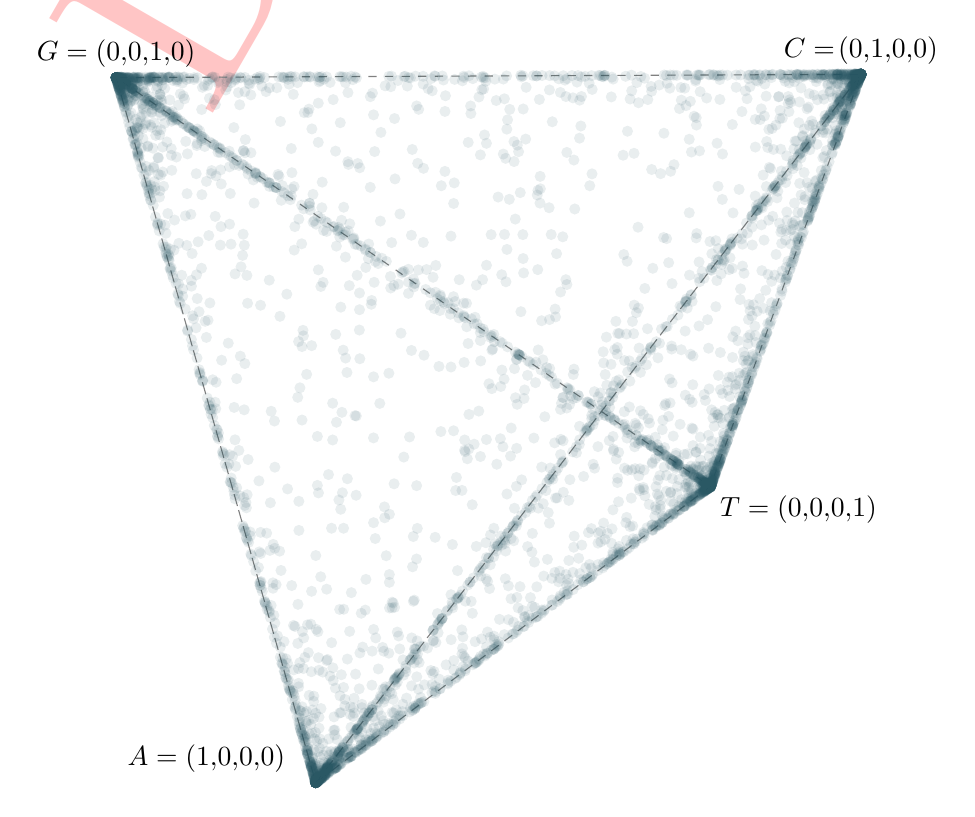
\begin{tikzpicture}[scale=10]


\begin{scope}[rotate around y=45,rotate around z=45]
 
% Draw the vertices of the tetrahedron

\coordinate (A) at (0, 0, 0);
\coordinate (C) at (1, 0, 0);
\coordinate (G) at (0.5, 0.866, 0);
\coordinate (T) at (0.5, 0.2887, 0.816);

%\foreach \p in {A,C,G,T}\fill[black] (\p) circle (0.02);

% Draw the edges of the cube
\draw[white!50!black, dashed]  (A) -- (C) -- (G) -- (A) -- (C) -- (T) -- (A) -- (T) -- (G) --  cycle;



    \pgfmathsetmacro{\alphaa}{0.1}       
       
\fill[color1,  opacity=\alphaa] (0.423,0.586,0.046) circle (.2pt);
         \fill[color1,  opacity=\alphaa] (0.984,0.027,0) circle (.2pt);
         \fill[color1,  opacity=\alphaa] (0.286,0.29,0.207) circle (.2pt);
         \fill[color1,  opacity=\alphaa] (0.842,0.106,0) circle (.2pt);
         \fill[color1,  opacity=\alphaa] (0.604,0.399,0.404) circle (.2pt);
         \fill[color1,  opacity=\alphaa] (0.093,0.02,0.057) circle (.2pt);
         \fill[color1,  opacity=\alphaa] (0,0,0) circle (.2pt);
         \fill[color1,  opacity=\alphaa] (0.231,0,0) circle (.2pt);
         \fill[color1,  opacity=\alphaa] (1,0,0) circle (.2pt);
         \fill[color1,  opacity=\alphaa] (0.36,0.556,0.003) circle (.2pt);
         \fill[color1,  opacity=\alphaa] (0.454,0.593,0.229) circle (.2pt);
         \fill[color1,  opacity=\alphaa] (0.506,0.85,0) circle (.2pt);
         \fill[color1,  opacity=\alphaa] (0.414,0.41,0.052) circle (.2pt);
         \fill[color1,  opacity=\alphaa] (0.533,0.269,0.762) circle (.2pt);
         \fill[color1,  opacity=\alphaa] (0.488,0.837,0) circle (.2pt);
         \fill[color1,  opacity=\alphaa] (0.001,0,0) circle (.2pt);
         \fill[color1,  opacity=\alphaa] (0.364,0.631,0) circle (.2pt);
         \fill[color1,  opacity=\alphaa] (0.495,0.836,0) circle (.2pt);
         \fill[color1,  opacity=\alphaa] (0.996,0.001,0) circle (.2pt);
         \fill[color1,  opacity=\alphaa] (0.999,0,0.001) circle (.2pt);
         \fill[color1,  opacity=\alphaa] (0.453,0.784,0) circle (.2pt);
         \fill[color1,  opacity=\alphaa] (0.405,0.235,0.66) circle (.2pt);
         \fill[color1,  opacity=\alphaa] (0.828,0.099,0.281) circle (.2pt);
         \fill[color1,  opacity=\alphaa] (0.648,0.186,0.526) circle (.2pt);
         \fill[color1,  opacity=\alphaa] (0.488,0.846,0) circle (.2pt);
         \fill[color1,  opacity=\alphaa] (0.47,0.438,0.499) circle (.2pt);
         \fill[color1,  opacity=\alphaa] (0.498,0.863,0) circle (.2pt);
         \fill[color1,  opacity=\alphaa] (0.006,0.01,0) circle (.2pt);
         \fill[color1,  opacity=\alphaa] (0.5,0.839,0.038) circle (.2pt);
         \fill[color1,  opacity=\alphaa] (0.605,0.051,0) circle (.2pt);
         \fill[color1,  opacity=\alphaa] (0.485,0.287,0.782) circle (.2pt);
         \fill[color1,  opacity=\alphaa] (0.516,0.502,0.418) circle (.2pt);
         \fill[color1,  opacity=\alphaa] (0.035,0.025,0.051) circle (.2pt);
         \fill[color1,  opacity=\alphaa] (0.5,0.289,0.816) circle (.2pt);
         \fill[color1,  opacity=\alphaa] (0.267,0.463,0) circle (.2pt);
         \fill[color1,  opacity=\alphaa] (0.5,0.289,0.816) circle (.2pt);
         \fill[color1,  opacity=\alphaa] (0.482,0.827,0) circle (.2pt);
         \fill[color1,  opacity=\alphaa] (0.5,0.298,0.804) circle (.2pt);
         \fill[color1,  opacity=\alphaa] (0.5,0.866,0) circle (.2pt);
         \fill[color1,  opacity=\alphaa] (0.5,0.289,0.816) circle (.2pt);
         \fill[color1,  opacity=\alphaa] (0.844,0.092,0.252) circle (.2pt);
         \fill[color1,  opacity=\alphaa] (0.476,0.583,0.341) circle (.2pt);
         \fill[color1,  opacity=\alphaa] (0.46,0.777,0.029) circle (.2pt);
         \fill[color1,  opacity=\alphaa] (0.996,0.007,0) circle (.2pt);
         \fill[color1,  opacity=\alphaa] (0.392,0.498,0.256) circle (.2pt);
         \fill[color1,  opacity=\alphaa] (0.977,0.013,0.038) circle (.2pt);
         \fill[color1,  opacity=\alphaa] (0.95,0.032,0.077) circle (.2pt);
         \fill[color1,  opacity=\alphaa] (0.436,0.611,0.002) circle (.2pt);
         \fill[color1,  opacity=\alphaa] (0.025,0.029,0.019) circle (.2pt);
         \fill[color1,  opacity=\alphaa] (0.952,0.028,0.079) circle (.2pt);
         \fill[color1,  opacity=\alphaa] (0.975,0.004,0.011) circle (.2pt);
         \fill[color1,  opacity=\alphaa] (0.006,0.002,0.006) circle (.2pt);
         \fill[color1,  opacity=\alphaa] (0.52,0.261,0.738) circle (.2pt);
         \fill[color1,  opacity=\alphaa] (0.319,0.184,0.521) circle (.2pt);
         \fill[color1,  opacity=\alphaa] (0.382,0.238,0.595) circle (.2pt);
         \fill[color1,  opacity=\alphaa] (0.207,0.357,0) circle (.2pt);
         \fill[color1,  opacity=\alphaa] (0.5,0.851,0.022) circle (.2pt);
         \fill[color1,  opacity=\alphaa] (0.575,0.22,0.616) circle (.2pt);
         \fill[color1,  opacity=\alphaa] (0.489,0.804,0.06) circle (.2pt);
         \fill[color1,  opacity=\alphaa] (0.968,0.006,0) circle (.2pt);
         \fill[color1,  opacity=\alphaa] (0.403,0,0) circle (.2pt);
         \fill[color1,  opacity=\alphaa] (0.008,0,0) circle (.2pt);
         \fill[color1,  opacity=\alphaa] (0.523,0.275,0.778) circle (.2pt);
         \fill[color1,  opacity=\alphaa] (0.5,0.474,0.554) circle (.2pt);
         \fill[color1,  opacity=\alphaa] (0.516,0.822,0.022) circle (.2pt);
         \fill[color1,  opacity=\alphaa] (0.021,0.001,0.003) circle (.2pt);
         \fill[color1,  opacity=\alphaa] (0.5,0.866,0) circle (.2pt);
         \fill[color1,  opacity=\alphaa] (0.339,0,0) circle (.2pt);
         \fill[color1,  opacity=\alphaa] (0.505,0.856,0.002) circle (.2pt);
         \fill[color1,  opacity=\alphaa] (0.002,0,0) circle (.2pt);
         \fill[color1,  opacity=\alphaa] (0.132,0.044,0.125) circle (.2pt);
         \fill[color1,  opacity=\alphaa] (0.508,0.851,0) circle (.2pt);
         \fill[color1,  opacity=\alphaa] (0,0,0) circle (.2pt);
         \fill[color1,  opacity=\alphaa] (0.831,0.29,0.003) circle (.2pt);
         \fill[color1,  opacity=\alphaa] (0,0,0) circle (.2pt);
         \fill[color1,  opacity=\alphaa] (0.502,0.301,0.793) circle (.2pt);
         \fill[color1,  opacity=\alphaa] (0.598,0.67,0.001) circle (.2pt);
         \fill[color1,  opacity=\alphaa] (0.5,0.846,0.028) circle (.2pt);
         \fill[color1,  opacity=\alphaa] (0.979,0.037,0) circle (.2pt);
         \fill[color1,  opacity=\alphaa] (0.548,0.78,0) circle (.2pt);
         \fill[color1,  opacity=\alphaa] (0.528,0.273,0.771) circle (.2pt);
         \fill[color1,  opacity=\alphaa] (0.445,0.769,0) circle (.2pt);
         \fill[color1,  opacity=\alphaa] (1,0,0) circle (.2pt);
         \fill[color1,  opacity=\alphaa] (0.461,0.264,0.748) circle (.2pt);
         \fill[color1,  opacity=\alphaa] (0.486,0.779,0.087) circle (.2pt);
         \fill[color1,  opacity=\alphaa] (0.074,0.018,0.034) circle (.2pt);
         \fill[color1,  opacity=\alphaa] (0.205,0.014,0.04) circle (.2pt);
         \fill[color1,  opacity=\alphaa] (0.501,0.288,0.815) circle (.2pt);
         \fill[color1,  opacity=\alphaa] (0.901,0.171,0) circle (.2pt);
         \fill[color1,  opacity=\alphaa] (0.5,0.305,0.793) circle (.2pt);
         \fill[color1,  opacity=\alphaa] (0.476,0.275,0.777) circle (.2pt);
         \fill[color1,  opacity=\alphaa] (0.563,0.749,0.011) circle (.2pt);
         \fill[color1,  opacity=\alphaa] (0.194,0.005,0.014) circle (.2pt);
         \fill[color1,  opacity=\alphaa] (0.5,0.289,0.816) circle (.2pt);
         \fill[color1,  opacity=\alphaa] (0.984,0,0) circle (.2pt);
         \fill[color1,  opacity=\alphaa] (0.97,0.016,0.013) circle (.2pt);
         \fill[color1,  opacity=\alphaa] (0.494,0.855,0) circle (.2pt);
         \fill[color1,  opacity=\alphaa] (0.497,0.287,0.811) circle (.2pt);
         \fill[color1,  opacity=\alphaa] (0.883,0.202,0) circle (.2pt);
         \fill[color1,  opacity=\alphaa] (0.305,0.055,0.001) circle (.2pt);
         \fill[color1,  opacity=\alphaa] (0.356,0.211,0.574) circle (.2pt);
         \fill[color1,  opacity=\alphaa] (0.02,0.035,0) circle (.2pt);
         \fill[color1,  opacity=\alphaa] (0.796,0.117,0.33) circle (.2pt);
         \fill[color1,  opacity=\alphaa] (0.391,0.161,0.43) circle (.2pt);
         \fill[color1,  opacity=\alphaa] (0.099,0.001,0) circle (.2pt);
         \fill[color1,  opacity=\alphaa] (0,0,0) circle (.2pt);
         \fill[color1,  opacity=\alphaa] (0.483,0.411,0.603) circle (.2pt);
         \fill[color1,  opacity=\alphaa] (0.5,0.289,0.816) circle (.2pt);
         \fill[color1,  opacity=\alphaa] (0.499,0.288,0.815) circle (.2pt);
         \fill[color1,  opacity=\alphaa] (0.499,0.864,0) circle (.2pt);
         \fill[color1,  opacity=\alphaa] (0.496,0.285,0.807) circle (.2pt);
         \fill[color1,  opacity=\alphaa] (0.493,0.852,0.002) circle (.2pt);
         \fill[color1,  opacity=\alphaa] (0.501,0.296,0.803) circle (.2pt);
         \fill[color1,  opacity=\alphaa] (0.155,0.26,0) circle (.2pt);
         \fill[color1,  opacity=\alphaa] (0.493,0.285,0.806) circle (.2pt);
         \fill[color1,  opacity=\alphaa] (0.581,0.14,0.377) circle (.2pt);
         \fill[color1,  opacity=\alphaa] (0.738,0,0) circle (.2pt);
         \fill[color1,  opacity=\alphaa] (0.655,0.199,0.563) circle (.2pt);
         \fill[color1,  opacity=\alphaa] (0.492,0.694,0.221) circle (.2pt);
         \fill[color1,  opacity=\alphaa] (0.502,0.86,0.004) circle (.2pt);
         \fill[color1,  opacity=\alphaa] (0.725,0.023,0.066) circle (.2pt);
         \fill[color1,  opacity=\alphaa] (0.029,0.049,0) circle (.2pt);
         \fill[color1,  opacity=\alphaa] (0.262,0,0) circle (.2pt);
         \fill[color1,  opacity=\alphaa] (0.382,0.368,0.414) circle (.2pt);
         \fill[color1,  opacity=\alphaa] (0.999,0.001,0.002) circle (.2pt);
         \fill[color1,  opacity=\alphaa] (0.5,0.313,0.783) circle (.2pt);
         \fill[color1,  opacity=\alphaa] (0.999,0,0) circle (.2pt);
         \fill[color1,  opacity=\alphaa] (0.496,0.858,0.001) circle (.2pt);
         \fill[color1,  opacity=\alphaa] (0.71,0.171,0.469) circle (.2pt);
         \fill[color1,  opacity=\alphaa] (0.025,0.014,0.041) circle (.2pt);
         \fill[color1,  opacity=\alphaa] (0.049,0,0) circle (.2pt);
         \fill[color1,  opacity=\alphaa] (0.439,0.15,0.424) circle (.2pt);
         \fill[color1,  opacity=\alphaa] (0.261,0.151,0.418) circle (.2pt);
         \fill[color1,  opacity=\alphaa] (0,0,0) circle (.2pt);
         \fill[color1,  opacity=\alphaa] (0.5,0.864,0.002) circle (.2pt);
         \fill[color1,  opacity=\alphaa] (0.347,0.427,0.242) circle (.2pt);
         \fill[color1,  opacity=\alphaa] (0.95,0.029,0.081) circle (.2pt);
         \fill[color1,  opacity=\alphaa] (1,0,0) circle (.2pt);
         \fill[color1,  opacity=\alphaa] (0.988,0.02,0) circle (.2pt);
         \fill[color1,  opacity=\alphaa] (0.784,0.124,0.35) circle (.2pt);
         \fill[color1,  opacity=\alphaa] (0.468,0.274,0.759) circle (.2pt);
         \fill[color1,  opacity=\alphaa] (0.286,0.093,0.263) circle (.2pt);
         \fill[color1,  opacity=\alphaa] (0.493,0.847,0.009) circle (.2pt);
         \fill[color1,  opacity=\alphaa] (0.927,0,0) circle (.2pt);
         \fill[color1,  opacity=\alphaa] (0.429,0,0) circle (.2pt);
         \fill[color1,  opacity=\alphaa] (0.916,0.047,0.133) circle (.2pt);
         \fill[color1,  opacity=\alphaa] (0.613,0,0.001) circle (.2pt);
         \fill[color1,  opacity=\alphaa] (0.5,0.327,0.763) circle (.2pt);
         \fill[color1,  opacity=\alphaa] (0.963,0.007,0) circle (.2pt);
         \fill[color1,  opacity=\alphaa] (0.534,0.268,0.759) circle (.2pt);
         \fill[color1,  opacity=\alphaa] (0.483,0.309,0.747) circle (.2pt);
         \fill[color1,  opacity=\alphaa] (0.499,0.865,0) circle (.2pt);
         \fill[color1,  opacity=\alphaa] (0.285,0.452,0.057) circle (.2pt);
         \fill[color1,  opacity=\alphaa] (0.848,0.088,0.247) circle (.2pt);
         \fill[color1,  opacity=\alphaa] (0.118,0.203,0.003) circle (.2pt);
         \fill[color1,  opacity=\alphaa] (1,0,0) circle (.2pt);
         \fill[color1,  opacity=\alphaa] (0.261,0.018,0.05) circle (.2pt);
         \fill[color1,  opacity=\alphaa] (0.5,0.866,0) circle (.2pt);
         \fill[color1,  opacity=\alphaa] (0.5,0.339,0.744) circle (.2pt);
         \fill[color1,  opacity=\alphaa] (0.066,0.113,0) circle (.2pt);
         \fill[color1,  opacity=\alphaa] (0.507,0.285,0.806) circle (.2pt);
         \fill[color1,  opacity=\alphaa] (0.023,0.004,0.01) circle (.2pt);
         \fill[color1,  opacity=\alphaa] (0.139,0.148,0) circle (.2pt);
         \fill[color1,  opacity=\alphaa] (0.507,0.332,0.74) circle (.2pt);
         \fill[color1,  opacity=\alphaa] (0.5,0.865,0.001) circle (.2pt);
         \fill[color1,  opacity=\alphaa] (0.5,0.301,0.799) circle (.2pt);
         \fill[color1,  opacity=\alphaa] (0.012,0.021,0) circle (.2pt);
         \fill[color1,  opacity=\alphaa] (0.459,0.767,0) circle (.2pt);
         \fill[color1,  opacity=\alphaa] (0.779,0.128,0.36) circle (.2pt);
         \fill[color1,  opacity=\alphaa] (0.5,0.699,0.236) circle (.2pt);
         \fill[color1,  opacity=\alphaa] (0.868,0.229,0) circle (.2pt);
         \fill[color1,  opacity=\alphaa] (0.004,0,0) circle (.2pt);
         \fill[color1,  opacity=\alphaa] (0.5,0.663,0.288) circle (.2pt);
         \fill[color1,  opacity=\alphaa] (0.496,0.507,0.498) circle (.2pt);
         \fill[color1,  opacity=\alphaa] (0.184,0.289,0.043) circle (.2pt);
         \fill[color1,  opacity=\alphaa] (0.5,0.863,0.004) circle (.2pt);
         \fill[color1,  opacity=\alphaa] (0.955,0.032,0.066) circle (.2pt);
         \fill[color1,  opacity=\alphaa] (0.484,0.838,0.002) circle (.2pt);
         \fill[color1,  opacity=\alphaa] (0.043,0.074,0) circle (.2pt);
         \fill[color1,  opacity=\alphaa] (0.501,0.31,0.784) circle (.2pt);
         \fill[color1,  opacity=\alphaa] (0.992,0.009,0) circle (.2pt);
         \fill[color1,  opacity=\alphaa] (0.491,0.851,0) circle (.2pt);
         \fill[color1,  opacity=\alphaa] (0.499,0.291,0.809) circle (.2pt);
         \fill[color1,  opacity=\alphaa] (0,0,0) circle (.2pt);
         \fill[color1,  opacity=\alphaa] (0.047,0.012,0.033) circle (.2pt);
         \fill[color1,  opacity=\alphaa] (0.961,0.067,0) circle (.2pt);
         \fill[color1,  opacity=\alphaa] (0.502,0.287,0.813) circle (.2pt);
         \fill[color1,  opacity=\alphaa] (0.499,0.288,0.814) circle (.2pt);
         \fill[color1,  opacity=\alphaa] (0.181,0.161,0) circle (.2pt);
         \fill[color1,  opacity=\alphaa] (0.455,0.783,0.001) circle (.2pt);
         \fill[color1,  opacity=\alphaa] (0.875,0,0) circle (.2pt);
         \fill[color1,  opacity=\alphaa] (0.505,0.304,0.782) circle (.2pt);
         \fill[color1,  opacity=\alphaa] (0.66,0.221,0.519) circle (.2pt);
         \fill[color1,  opacity=\alphaa] (0.564,0.252,0.712) circle (.2pt);
         \fill[color1,  opacity=\alphaa] (0.5,0.289,0.816) circle (.2pt);
         \fill[color1,  opacity=\alphaa] (0.5,0.289,0.816) circle (.2pt);
         \fill[color1,  opacity=\alphaa] (0.667,0.325,0.355) circle (.2pt);
         \fill[color1,  opacity=\alphaa] (1,0,0) circle (.2pt);
         \fill[color1,  opacity=\alphaa] (0.406,0.454,0.29) circle (.2pt);
         \fill[color1,  opacity=\alphaa] (0.55,0.776,0.004) circle (.2pt);
         \fill[color1,  opacity=\alphaa] (0.309,0.179,0.505) circle (.2pt);
         \fill[color1,  opacity=\alphaa] (0.5,0.861,0.007) circle (.2pt);
         \fill[color1,  opacity=\alphaa] (0.47,0.723,0.127) circle (.2pt);
         \fill[color1,  opacity=\alphaa] (0.061,0.03,0.083) circle (.2pt);
         \fill[color1,  opacity=\alphaa] (1,0,0) circle (.2pt);
         \fill[color1,  opacity=\alphaa] (0.5,0.288,0.816) circle (.2pt);
         \fill[color1,  opacity=\alphaa] (0.001,0,0) circle (.2pt);
         \fill[color1,  opacity=\alphaa] (0.5,0.865,0) circle (.2pt);
         \fill[color1,  opacity=\alphaa] (0.883,0.203,0) circle (.2pt);
         \fill[color1,  opacity=\alphaa] (0.224,0,0) circle (.2pt);
         \fill[color1,  opacity=\alphaa] (0.849,0.234,0) circle (.2pt);
         \fill[color1,  opacity=\alphaa] (0.484,0,0) circle (.2pt);
         \fill[color1,  opacity=\alphaa] (0.732,0.154,0.437) circle (.2pt);
         \fill[color1,  opacity=\alphaa] (0.998,0.001,0.004) circle (.2pt);
         \fill[color1,  opacity=\alphaa] (0.46,0.424,0.526) circle (.2pt);
         \fill[color1,  opacity=\alphaa] (0.524,0.825,0) circle (.2pt);
         \fill[color1,  opacity=\alphaa] (0.531,0.026,0.054) circle (.2pt);
         \fill[color1,  opacity=\alphaa] (0.022,0.001,0) circle (.2pt);
         \fill[color1,  opacity=\alphaa] (0.733,0.037,0.099) circle (.2pt);
         \fill[color1,  opacity=\alphaa] (0.5,0.339,0.745) circle (.2pt);
         \fill[color1,  opacity=\alphaa] (0.993,0.013,0) circle (.2pt);
         \fill[color1,  opacity=\alphaa] (0.5,0.857,0.013) circle (.2pt);
         \fill[color1,  opacity=\alphaa] (0.995,0.001,0.001) circle (.2pt);
         \fill[color1,  opacity=\alphaa] (0.075,0.103,0.039) circle (.2pt);
         \fill[color1,  opacity=\alphaa] (0.994,0.003,0.009) circle (.2pt);
         \fill[color1,  opacity=\alphaa] (0.855,0.021,0) circle (.2pt);
         \fill[color1,  opacity=\alphaa] (0.5,0.856,0.014) circle (.2pt);
         \fill[color1,  opacity=\alphaa] (0.995,0.003,0.008) circle (.2pt);
         \fill[color1,  opacity=\alphaa] (1,0,0) circle (.2pt);
         \fill[color1,  opacity=\alphaa] (0.002,0.001,0) circle (.2pt);
         \fill[color1,  opacity=\alphaa] (0.994,0,0.001) circle (.2pt);
         \fill[color1,  opacity=\alphaa] (0.493,0.281,0.794) circle (.2pt);
         \fill[color1,  opacity=\alphaa] (0.825,0.303,0) circle (.2pt);
         \fill[color1,  opacity=\alphaa] (0.501,0.859,0.008) circle (.2pt);
         \fill[color1,  opacity=\alphaa] (0.496,0.286,0.808) circle (.2pt);
         \fill[color1,  opacity=\alphaa] (0.497,0.283,0.799) circle (.2pt);
         \fill[color1,  opacity=\alphaa] (0.501,0.288,0.814) circle (.2pt);
         \fill[color1,  opacity=\alphaa] (0.502,0.298,0.798) circle (.2pt);
         \fill[color1,  opacity=\alphaa] (0.229,0.059,0.017) circle (.2pt);
         \fill[color1,  opacity=\alphaa] (0.5,0.858,0.011) circle (.2pt);
         \fill[color1,  opacity=\alphaa] (0.5,0.866,0) circle (.2pt);
         \fill[color1,  opacity=\alphaa] (0.17,0.06,0) circle (.2pt);
         \fill[color1,  opacity=\alphaa] (0.398,0.686,0.006) circle (.2pt);
         \fill[color1,  opacity=\alphaa] (0.949,0.071,0) circle (.2pt);
         \fill[color1,  opacity=\alphaa] (0.5,0.289,0.816) circle (.2pt);
         \fill[color1,  opacity=\alphaa] (0.976,0.03,0) circle (.2pt);
         \fill[color1,  opacity=\alphaa] (0.286,0.109,0.003) circle (.2pt);
         \fill[color1,  opacity=\alphaa] (0.002,0.001,0.002) circle (.2pt);
         \fill[color1,  opacity=\alphaa] (0.345,0.559,0) circle (.2pt);
         \fill[color1,  opacity=\alphaa] (0.456,0.633,0.219) circle (.2pt);
         \fill[color1,  opacity=\alphaa] (0.499,0.833,0.045) circle (.2pt);
         \fill[color1,  opacity=\alphaa] (0.01,0.005,0.002) circle (.2pt);
         \fill[color1,  opacity=\alphaa] (0.491,0.33,0.735) circle (.2pt);
         \fill[color1,  opacity=\alphaa] (0.554,0.752,0) circle (.2pt);
         \fill[color1,  opacity=\alphaa] (0.493,0.854,0) circle (.2pt);
         \fill[color1,  opacity=\alphaa] (0.999,0.001,0) circle (.2pt);
         \fill[color1,  opacity=\alphaa] (0.984,0.028,0) circle (.2pt);
         \fill[color1,  opacity=\alphaa] (0.999,0,0) circle (.2pt);
         \fill[color1,  opacity=\alphaa] (0.071,0.041,0.117) circle (.2pt);
         \fill[color1,  opacity=\alphaa] (0,0,0) circle (.2pt);
         \fill[color1,  opacity=\alphaa] (0.572,0.649,0.13) circle (.2pt);
         \fill[color1,  opacity=\alphaa] (0.406,0.235,0.662) circle (.2pt);
         \fill[color1,  opacity=\alphaa] (0.001,0.001,0.001) circle (.2pt);
         \fill[color1,  opacity=\alphaa] (0.998,0.001,0.003) circle (.2pt);
         \fill[color1,  opacity=\alphaa] (0.334,0,0) circle (.2pt);
         \fill[color1,  opacity=\alphaa] (0.989,0,0) circle (.2pt);
         \fill[color1,  opacity=\alphaa] (0.716,0.485,0.005) circle (.2pt);
         \fill[color1,  opacity=\alphaa] (0.002,0.004,0) circle (.2pt);
         \fill[color1,  opacity=\alphaa] (0.948,0.033,0.08) circle (.2pt);
         \fill[color1,  opacity=\alphaa] (0.996,0.002,0.007) circle (.2pt);
         \fill[color1,  opacity=\alphaa] (0.03,0.048,0) circle (.2pt);
         \fill[color1,  opacity=\alphaa] (0.503,0.335,0.744) circle (.2pt);
         \fill[color1,  opacity=\alphaa] (0.241,0.001,0) circle (.2pt);
         \fill[color1,  opacity=\alphaa] (0.063,0,0) circle (.2pt);
         \fill[color1,  opacity=\alphaa] (0.5,0.289,0.816) circle (.2pt);
         \fill[color1,  opacity=\alphaa] (0,0,0) circle (.2pt);
         \fill[color1,  opacity=\alphaa] (0.026,0,0) circle (.2pt);
         \fill[color1,  opacity=\alphaa] (0.021,0.037,0) circle (.2pt);
         \fill[color1,  opacity=\alphaa] (0.511,0.836,0.013) circle (.2pt);
         \fill[color1,  opacity=\alphaa] (0.953,0.027,0.076) circle (.2pt);
         \fill[color1,  opacity=\alphaa] (0.013,0,0) circle (.2pt);
         \fill[color1,  opacity=\alphaa] (0.452,0.288,0.7) circle (.2pt);
         \fill[color1,  opacity=\alphaa] (0.004,0.002,0.006) circle (.2pt);
         \fill[color1,  opacity=\alphaa] (0.455,0.055,0) circle (.2pt);
         \fill[color1,  opacity=\alphaa] (0.775,0.13,0.367) circle (.2pt);
         \fill[color1,  opacity=\alphaa] (0.5,0.289,0.816) circle (.2pt);
         \fill[color1,  opacity=\alphaa] (0.841,0,0) circle (.2pt);
         \fill[color1,  opacity=\alphaa] (0.732,0.004,0.009) circle (.2pt);
         \fill[color1,  opacity=\alphaa] (0.488,0.282,0.797) circle (.2pt);
         \fill[color1,  opacity=\alphaa] (0.003,0.005,0) circle (.2pt);
         \fill[color1,  opacity=\alphaa] (0.5,0.866,0.001) circle (.2pt);
         \fill[color1,  opacity=\alphaa] (0.513,0.281,0.796) circle (.2pt);
         \fill[color1,  opacity=\alphaa] (0.497,0.31,0.778) circle (.2pt);
         \fill[color1,  opacity=\alphaa] (0.83,0.289,0.007) circle (.2pt);
         \fill[color1,  opacity=\alphaa] (0.501,0.288,0.814) circle (.2pt);
         \fill[color1,  opacity=\alphaa] (0.5,0.29,0.815) circle (.2pt);
         \fill[color1,  opacity=\alphaa] (0.971,0.02,0.041) circle (.2pt);
         \fill[color1,  opacity=\alphaa] (0,0,0) circle (.2pt);
         \fill[color1,  opacity=\alphaa] (0.513,0.82,0.034) circle (.2pt);
         \fill[color1,  opacity=\alphaa] (0.518,0.67,0.234) circle (.2pt);
         \fill[color1,  opacity=\alphaa] (0.989,0.006,0.018) circle (.2pt);
         \fill[color1,  opacity=\alphaa] (1,0,0) circle (.2pt);
         \fill[color1,  opacity=\alphaa] (0.5,0.854,0.017) circle (.2pt);
         \fill[color1,  opacity=\alphaa] (0.501,0.797,0.059) circle (.2pt);
         \fill[color1,  opacity=\alphaa] (0.783,0.139,0.335) circle (.2pt);
         \fill[color1,  opacity=\alphaa] (0.194,0.135,0.01) circle (.2pt);
         \fill[color1,  opacity=\alphaa] (0.504,0.86,0) circle (.2pt);
         \fill[color1,  opacity=\alphaa] (0.915,0.049,0.139) circle (.2pt);
         \fill[color1,  opacity=\alphaa] (0.006,0.003,0.01) circle (.2pt);
         \fill[color1,  opacity=\alphaa] (0.5,0.393,0.669) circle (.2pt);
         \fill[color1,  opacity=\alphaa] (0.001,0,0.001) circle (.2pt);
         \fill[color1,  opacity=\alphaa] (0.916,0.089,0.065) circle (.2pt);
         \fill[color1,  opacity=\alphaa] (0.003,0,0) circle (.2pt);
         \fill[color1,  opacity=\alphaa] (0.552,0.216,0.612) circle (.2pt);
         \fill[color1,  opacity=\alphaa] (0.987,0.023,0) circle (.2pt);
         \fill[color1,  opacity=\alphaa] (0.883,0,0) circle (.2pt);
         \fill[color1,  opacity=\alphaa] (0.362,0,0) circle (.2pt);
         \fill[color1,  opacity=\alphaa] (0.952,0.003,0.003) circle (.2pt);
         \fill[color1,  opacity=\alphaa] (0.091,0.151,0.009) circle (.2pt);
         \fill[color1,  opacity=\alphaa] (0.426,0.733,0.007) circle (.2pt);
         \fill[color1,  opacity=\alphaa] (0.5,0.861,0.007) circle (.2pt);
         \fill[color1,  opacity=\alphaa] (0.5,0.289,0.816) circle (.2pt);
         \fill[color1,  opacity=\alphaa] (0.62,0.658,0) circle (.2pt);
         \fill[color1,  opacity=\alphaa] (0.785,0.341,0.044) circle (.2pt);
         \fill[color1,  opacity=\alphaa] (0.004,0.007,0) circle (.2pt);
         \fill[color1,  opacity=\alphaa] (0.702,0.185,0.416) circle (.2pt);
         \fill[color1,  opacity=\alphaa] (0.071,0.041,0.116) circle (.2pt);
         \fill[color1,  opacity=\alphaa] (0.498,0.311,0.781) circle (.2pt);
         \fill[color1,  opacity=\alphaa] (0.499,0.86,0.006) circle (.2pt);
         \fill[color1,  opacity=\alphaa] (0.508,0.85,0) circle (.2pt);
         \fill[color1,  opacity=\alphaa] (0.006,0,0) circle (.2pt);
         \fill[color1,  opacity=\alphaa] (0.523,0.826,0) circle (.2pt);
         \fill[color1,  opacity=\alphaa] (0.001,0,0) circle (.2pt);
         \fill[color1,  opacity=\alphaa] (0.49,0.087,0.243) circle (.2pt);
         \fill[color1,  opacity=\alphaa] (0.5,0.857,0.013) circle (.2pt);
         \fill[color1,  opacity=\alphaa] (0.5,0.771,0.134) circle (.2pt);
         \fill[color1,  opacity=\alphaa] (0.444,0.365,0.572) circle (.2pt);
         \fill[color1,  opacity=\alphaa] (0.313,0.175,0.494) circle (.2pt);
         \fill[color1,  opacity=\alphaa] (0.497,0.287,0.812) circle (.2pt);
         \fill[color1,  opacity=\alphaa] (0.167,0.096,0.273) circle (.2pt);
         \fill[color1,  opacity=\alphaa] (0.5,0.528,0.477) circle (.2pt);
         \fill[color1,  opacity=\alphaa] (0.473,0.791,0.039) circle (.2pt);
         \fill[color1,  opacity=\alphaa] (0.892,0.187,0) circle (.2pt);
         \fill[color1,  opacity=\alphaa] (0.187,0.003,0) circle (.2pt);
         \fill[color1,  opacity=\alphaa] (0.497,0.857,0) circle (.2pt);
         \fill[color1,  opacity=\alphaa] (1,0,0) circle (.2pt);
         \fill[color1,  opacity=\alphaa] (0.031,0.018,0.051) circle (.2pt);
         \fill[color1,  opacity=\alphaa] (0.495,0.857,0) circle (.2pt);
         \fill[color1,  opacity=\alphaa] (0.807,0.3,0) circle (.2pt);
         \fill[color1,  opacity=\alphaa] (0.226,0.131,0.37) circle (.2pt);
         \fill[color1,  opacity=\alphaa] (0.984,0,0) circle (.2pt);
         \fill[color1,  opacity=\alphaa] (0.498,0.288,0.813) circle (.2pt);
         \fill[color1,  opacity=\alphaa] (0.011,0.019,0) circle (.2pt);
         \fill[color1,  opacity=\alphaa] (0.5,0.289,0.816) circle (.2pt);
         \fill[color1,  opacity=\alphaa] (0.936,0.11,0) circle (.2pt);
         \fill[color1,  opacity=\alphaa] (0.491,0.283,0.801) circle (.2pt);
         \fill[color1,  opacity=\alphaa] (0.419,0.242,0.675) circle (.2pt);
         \fill[color1,  opacity=\alphaa] (0.538,0.267,0.754) circle (.2pt);
         \fill[color1,  opacity=\alphaa] (0.501,0.288,0.814) circle (.2pt);
         \fill[color1,  opacity=\alphaa] (0.5,0.355,0.722) circle (.2pt);
         \fill[color1,  opacity=\alphaa] (0,0.001,0) circle (.2pt);
         \fill[color1,  opacity=\alphaa] (0.286,0.165,0.467) circle (.2pt);
         \fill[color1,  opacity=\alphaa] (0.5,0.67,0.277) circle (.2pt);
         \fill[color1,  opacity=\alphaa] (0.03,0,0) circle (.2pt);
         \fill[color1,  opacity=\alphaa] (0.072,0.035,0.099) circle (.2pt);
         \fill[color1,  opacity=\alphaa] (0.491,0.283,0.8) circle (.2pt);
         \fill[color1,  opacity=\alphaa] (0.113,0.146,0) circle (.2pt);
         \fill[color1,  opacity=\alphaa] (0.5,0.445,0.594) circle (.2pt);
         \fill[color1,  opacity=\alphaa] (0.246,0.426,0) circle (.2pt);
         \fill[color1,  opacity=\alphaa] (0.528,0.219,0.618) circle (.2pt);
         \fill[color1,  opacity=\alphaa] (0.985,0.012,0.021) circle (.2pt);
         \fill[color1,  opacity=\alphaa] (0.503,0.291,0.803) circle (.2pt);
         \fill[color1,  opacity=\alphaa] (0.5,0.85,0.023) circle (.2pt);
         \fill[color1,  opacity=\alphaa] (0.201,0.339,0.012) circle (.2pt);
         \fill[color1,  opacity=\alphaa] (0.5,0.766,0.141) circle (.2pt);
         \fill[color1,  opacity=\alphaa] (0.069,0.075,0.063) circle (.2pt);
         \fill[color1,  opacity=\alphaa] (0.999,0,0.001) circle (.2pt);
         \fill[color1,  opacity=\alphaa] (0.722,0.161,0.454) circle (.2pt);
         \fill[color1,  opacity=\alphaa] (0.501,0.3,0.798) circle (.2pt);
         \fill[color1,  opacity=\alphaa] (0.264,0.153,0.432) circle (.2pt);
         \fill[color1,  opacity=\alphaa] (0.077,0,0) circle (.2pt);
         \fill[color1,  opacity=\alphaa] (0.812,0.088,0.239) circle (.2pt);
         \fill[color1,  opacity=\alphaa] (0.565,0.488,0.376) circle (.2pt);
         \fill[color1,  opacity=\alphaa] (0.968,0.055,0) circle (.2pt);
         \fill[color1,  opacity=\alphaa] (0,0,0.001) circle (.2pt);
         \fill[color1,  opacity=\alphaa] (0.526,0.822,0) circle (.2pt);
         \fill[color1,  opacity=\alphaa] (0.467,0.27,0.762) circle (.2pt);
         \fill[color1,  opacity=\alphaa] (0.025,0,0) circle (.2pt);
         \fill[color1,  opacity=\alphaa] (0.5,0.325,0.765) circle (.2pt);
         \fill[color1,  opacity=\alphaa] (0.257,0.301,0.143) circle (.2pt);
         \fill[color1,  opacity=\alphaa] (0.009,0,0.001) circle (.2pt);
         \fill[color1,  opacity=\alphaa] (0.686,0.53,0.019) circle (.2pt);
         \fill[color1,  opacity=\alphaa] (0.5,0.866,0) circle (.2pt);
         \fill[color1,  opacity=\alphaa] (0.735,0.191,0.38) circle (.2pt);
         \fill[color1,  opacity=\alphaa] (0.499,0.864,0) circle (.2pt);
         \fill[color1,  opacity=\alphaa] (0,0,0) circle (.2pt);
         \fill[color1,  opacity=\alphaa] (0.971,0.051,0) circle (.2pt);
         \fill[color1,  opacity=\alphaa] (0.934,0.047,0) circle (.2pt);
         \fill[color1,  opacity=\alphaa] (0.5,0.501,0.517) circle (.2pt);
         \fill[color1,  opacity=\alphaa] (0.125,0.189,0.037) circle (.2pt);
         \fill[color1,  opacity=\alphaa] (0.5,0.861,0.006) circle (.2pt);
         \fill[color1,  opacity=\alphaa] (0.5,0.788,0.109) circle (.2pt);
         \fill[color1,  opacity=\alphaa] (0.003,0.003,0.002) circle (.2pt);
         \fill[color1,  opacity=\alphaa] (0.501,0.865,0) circle (.2pt);
         \fill[color1,  opacity=\alphaa] (0.931,0.072,0.012) circle (.2pt);
         \fill[color1,  opacity=\alphaa] (0.5,0.865,0) circle (.2pt);
         \fill[color1,  opacity=\alphaa] (1,0.001,0) circle (.2pt);
         \fill[color1,  opacity=\alphaa] (0.004,0.007,0) circle (.2pt);
         \fill[color1,  opacity=\alphaa] (0.237,0.395,0) circle (.2pt);
         \fill[color1,  opacity=\alphaa] (0.499,0.294,0.807) circle (.2pt);
         \fill[color1,  opacity=\alphaa] (0.516,0.28,0.791) circle (.2pt);
         \fill[color1,  opacity=\alphaa] (0.461,0.172,0.486) circle (.2pt);
         \fill[color1,  opacity=\alphaa] (0.454,0.262,0.741) circle (.2pt);
         \fill[color1,  opacity=\alphaa] (0.013,0,0) circle (.2pt);
         \fill[color1,  opacity=\alphaa] (0.409,0.238,0.665) circle (.2pt);
         \fill[color1,  opacity=\alphaa] (0.5,0.866,0) circle (.2pt);
         \fill[color1,  opacity=\alphaa] (0.485,0.363,0.674) circle (.2pt);
         \fill[color1,  opacity=\alphaa] (0.489,0.417,0.608) circle (.2pt);
         \fill[color1,  opacity=\alphaa] (1,0,0) circle (.2pt);
         \fill[color1,  opacity=\alphaa] (0.001,0.001,0) circle (.2pt);
         \fill[color1,  opacity=\alphaa] (0.497,0.287,0.812) circle (.2pt);
         \fill[color1,  opacity=\alphaa] (0.037,0.005,0.014) circle (.2pt);
         \fill[color1,  opacity=\alphaa] (0.85,0.084,0.237) circle (.2pt);
         \fill[color1,  opacity=\alphaa] (0.46,0.537,0.286) circle (.2pt);
         \fill[color1,  opacity=\alphaa] (0.5,0.289,0.816) circle (.2pt);
         \fill[color1,  opacity=\alphaa] (0.5,0.289,0.816) circle (.2pt);
         \fill[color1,  opacity=\alphaa] (0.488,0.843,0.003) circle (.2pt);
         \fill[color1,  opacity=\alphaa] (0.482,0.278,0.783) circle (.2pt);
         \fill[color1,  opacity=\alphaa] (0.54,0.318,0.677) circle (.2pt);
         \fill[color1,  opacity=\alphaa] (0.5,0.289,0.816) circle (.2pt);
         \fill[color1,  opacity=\alphaa] (0.491,0.808,0) circle (.2pt);
         \fill[color1,  opacity=\alphaa] (0.727,0,0) circle (.2pt);
         \fill[color1,  opacity=\alphaa] (0,0,0) circle (.2pt);
         \fill[color1,  opacity=\alphaa] (0.699,0.174,0.491) circle (.2pt);
         \fill[color1,  opacity=\alphaa] (0,0,0) circle (.2pt);
         \fill[color1,  opacity=\alphaa] (0.5,0.865,0.001) circle (.2pt);
         \fill[color1,  opacity=\alphaa] (0.996,0.006,0.001) circle (.2pt);
         \fill[color1,  opacity=\alphaa] (0.901,0.172,0) circle (.2pt);
         \fill[color1,  opacity=\alphaa] (0.466,0.64,0.236) circle (.2pt);
         \fill[color1,  opacity=\alphaa] (0.062,0.034,0.094) circle (.2pt);
         \fill[color1,  opacity=\alphaa] (0.986,0.023,0) circle (.2pt);
         \fill[color1,  opacity=\alphaa] (0.997,0.002,0.005) circle (.2pt);
         \fill[color1,  opacity=\alphaa] (0.499,0.288,0.814) circle (.2pt);
         \fill[color1,  opacity=\alphaa] (0.963,0,0) circle (.2pt);
         \fill[color1,  opacity=\alphaa] (0,0,0) circle (.2pt);
         \fill[color1,  opacity=\alphaa] (0.354,0.339,0.387) circle (.2pt);
         \fill[color1,  opacity=\alphaa] (0.471,0.372,0.628) circle (.2pt);
         \fill[color1,  opacity=\alphaa] (0.971,0.017,0.046) circle (.2pt);
         \fill[color1,  opacity=\alphaa] (0.49,0.281,0.795) circle (.2pt);
         \fill[color1,  opacity=\alphaa] (0.583,0.722,0.001) circle (.2pt);
         \fill[color1,  opacity=\alphaa] (0.487,0.844,0) circle (.2pt);
         \fill[color1,  opacity=\alphaa] (0.129,0.217,0.01) circle (.2pt);
         \fill[color1,  opacity=\alphaa] (0.998,0,0) circle (.2pt);
         \fill[color1,  opacity=\alphaa] (0.504,0.86,0) circle (.2pt);
         \fill[color1,  opacity=\alphaa] (0,0,0) circle (.2pt);
         \fill[color1,  opacity=\alphaa] (0.5,0.289,0.816) circle (.2pt);
         \fill[color1,  opacity=\alphaa] (0.896,0.002,0.005) circle (.2pt);
         \fill[color1,  opacity=\alphaa] (0.961,0.066,0.002) circle (.2pt);
         \fill[color1,  opacity=\alphaa] (0.554,0.313,0.651) circle (.2pt);
         \fill[color1,  opacity=\alphaa] (0.502,0.861,0) circle (.2pt);
         \fill[color1,  opacity=\alphaa] (0.587,0.278,0.609) circle (.2pt);
         \fill[color1,  opacity=\alphaa] (0.487,0.819,0.033) circle (.2pt);
         \fill[color1,  opacity=\alphaa] (0.457,0.791,0) circle (.2pt);
         \fill[color1,  opacity=\alphaa] (0.5,0.425,0.623) circle (.2pt);
         \fill[color1,  opacity=\alphaa] (0.426,0.235,0.663) circle (.2pt);
         \fill[color1,  opacity=\alphaa] (0.511,0,0) circle (.2pt);
         \fill[color1,  opacity=\alphaa] (0.023,0,0) circle (.2pt);
         \fill[color1,  opacity=\alphaa] (0.518,0.829,0.009) circle (.2pt);
         \fill[color1,  opacity=\alphaa] (0.877,0.002,0) circle (.2pt);
         \fill[color1,  opacity=\alphaa] (0.604,0.228,0.646) circle (.2pt);
         \fill[color1,  opacity=\alphaa] (0.027,0.042,0) circle (.2pt);
         \fill[color1,  opacity=\alphaa] (0.976,0.039,0) circle (.2pt);
         \fill[color1,  opacity=\alphaa] (0.497,0.291,0.806) circle (.2pt);
         \fill[color1,  opacity=\alphaa] (0.496,0.571,0.406) circle (.2pt);
         \fill[color1,  opacity=\alphaa] (0.558,0.371,0.385) circle (.2pt);
         \fill[color1,  opacity=\alphaa] (0.5,0.35,0.729) circle (.2pt);
         \fill[color1,  opacity=\alphaa] (0.268,0.265,0) circle (.2pt);
         \fill[color1,  opacity=\alphaa] (0.015,0.025,0) circle (.2pt);
         \fill[color1,  opacity=\alphaa] (0.487,0.449,0.558) circle (.2pt);
         \fill[color1,  opacity=\alphaa] (1,0,0) circle (.2pt);
         \fill[color1,  opacity=\alphaa] (0.989,0.006,0.017) circle (.2pt);
         \fill[color1,  opacity=\alphaa] (0.442,0.489,0.391) circle (.2pt);
         \fill[color1,  opacity=\alphaa] (0.508,0.85,0.003) circle (.2pt);
         \fill[color1,  opacity=\alphaa] (0.124,0.024,0.067) circle (.2pt);
         \fill[color1,  opacity=\alphaa] (0.121,0,0) circle (.2pt);
         \fill[color1,  opacity=\alphaa] (0.501,0.289,0.815) circle (.2pt);
         \fill[color1,  opacity=\alphaa] (0.496,0.778,0.115) circle (.2pt);
         \fill[color1,  opacity=\alphaa] (0,0,0) circle (.2pt);
         \fill[color1,  opacity=\alphaa] (0.047,0.064,0) circle (.2pt);
         \fill[color1,  opacity=\alphaa] (0.919,0.14,0) circle (.2pt);
         \fill[color1,  opacity=\alphaa] (0.925,0.129,0) circle (.2pt);
         \fill[color1,  opacity=\alphaa] (0.536,0.805,0) circle (.2pt);
         \fill[color1,  opacity=\alphaa] (0.996,0,0) circle (.2pt);
         \fill[color1,  opacity=\alphaa] (0.517,0.391,0.63) circle (.2pt);
         \fill[color1,  opacity=\alphaa] (0.459,0.267,0.747) circle (.2pt);
         \fill[color1,  opacity=\alphaa] (0.673,0.124,0.352) circle (.2pt);
         \fill[color1,  opacity=\alphaa] (0.036,0.062,0) circle (.2pt);
         \fill[color1,  opacity=\alphaa] (0.5,0.289,0.816) circle (.2pt);
         \fill[color1,  opacity=\alphaa] (0.184,0.103,0.293) circle (.2pt);
         \fill[color1,  opacity=\alphaa] (0.508,0.298,0.785) circle (.2pt);
         \fill[color1,  opacity=\alphaa] (0.5,0.289,0.816) circle (.2pt);
         \fill[color1,  opacity=\alphaa] (0.5,0.866,0) circle (.2pt);
         \fill[color1,  opacity=\alphaa] (0.732,0.412,0.057) circle (.2pt);
         \fill[color1,  opacity=\alphaa] (0.953,0.018,0.05) circle (.2pt);
         \fill[color1,  opacity=\alphaa] (0.467,0.776,0.045) circle (.2pt);
         \fill[color1,  opacity=\alphaa] (0.281,0.306,0.255) circle (.2pt);
         \fill[color1,  opacity=\alphaa] (0.905,0.134,0) circle (.2pt);
         \fill[color1,  opacity=\alphaa] (0,0,0) circle (.2pt);
         \fill[color1,  opacity=\alphaa] (0.974,0.044,0.001) circle (.2pt);
         \fill[color1,  opacity=\alphaa] (0.5,0.427,0.621) circle (.2pt);
         \fill[color1,  opacity=\alphaa] (0.577,0.517,0) circle (.2pt);
         \fill[color1,  opacity=\alphaa] (0.491,0.587,0.371) circle (.2pt);
         \fill[color1,  opacity=\alphaa] (0.737,0.456,0) circle (.2pt);
         \fill[color1,  opacity=\alphaa] (0.5,0.289,0.816) circle (.2pt);
         \fill[color1,  opacity=\alphaa] (0.96,0.066,0) circle (.2pt);
         \fill[color1,  opacity=\alphaa] (0.901,0,0) circle (.2pt);
         \fill[color1,  opacity=\alphaa] (0.5,0.862,0.006) circle (.2pt);
         \fill[color1,  opacity=\alphaa] (0.023,0.039,0) circle (.2pt);
         \fill[color1,  opacity=\alphaa] (0.081,0.075,0.091) circle (.2pt);
         \fill[color1,  opacity=\alphaa] (0.719,0.162,0.458) circle (.2pt);
         \fill[color1,  opacity=\alphaa] (0.5,0.289,0.816) circle (.2pt);
         \fill[color1,  opacity=\alphaa] (0.034,0.059,0) circle (.2pt);
         \fill[color1,  opacity=\alphaa] (0.753,0.143,0.404) circle (.2pt);
         \fill[color1,  opacity=\alphaa] (0.483,0.837,0) circle (.2pt);
         \fill[color1,  opacity=\alphaa] (0.042,0.049,0) circle (.2pt);
         \fill[color1,  opacity=\alphaa] (0.968,0.054,0.001) circle (.2pt);
         \fill[color1,  opacity=\alphaa] (0.153,0.084,0.236) circle (.2pt);
         \fill[color1,  opacity=\alphaa] (1,0,0) circle (.2pt);
         \fill[color1,  opacity=\alphaa] (0.499,0.289,0.815) circle (.2pt);
         \fill[color1,  opacity=\alphaa] (0.002,0.002,0) circle (.2pt);
         \fill[color1,  opacity=\alphaa] (0.5,0.289,0.816) circle (.2pt);
         \fill[color1,  opacity=\alphaa] (0.5,0.619,0.349) circle (.2pt);
         \fill[color1,  opacity=\alphaa] (0.499,0.811,0.077) circle (.2pt);
         \fill[color1,  opacity=\alphaa] (1,0,0) circle (.2pt);
         \fill[color1,  opacity=\alphaa] (0.109,0.104,0.119) circle (.2pt);
         \fill[color1,  opacity=\alphaa] (0.484,0.838,0) circle (.2pt);
         \fill[color1,  opacity=\alphaa] (0.216,0.124,0) circle (.2pt);
         \fill[color1,  opacity=\alphaa] (0.017,0,0) circle (.2pt);
         \fill[color1,  opacity=\alphaa] (0.919,0.003,0) circle (.2pt);
         \fill[color1,  opacity=\alphaa] (0.637,0.625,0.005) circle (.2pt);
         \fill[color1,  opacity=\alphaa] (0.5,0.837,0.041) circle (.2pt);
         \fill[color1,  opacity=\alphaa] (0.524,0.819,0.009) circle (.2pt);
         \fill[color1,  opacity=\alphaa] (1,0,0) circle (.2pt);
         \fill[color1,  opacity=\alphaa] (0.96,0.031,0.053) circle (.2pt);
         \fill[color1,  opacity=\alphaa] (0.109,0.189,0.001) circle (.2pt);
         \fill[color1,  opacity=\alphaa] (0.818,0.209,0.151) circle (.2pt);
         \fill[color1,  opacity=\alphaa] (0.021,0.015,0.031) circle (.2pt);
         \fill[color1,  opacity=\alphaa] (0.5,0.796,0.099) circle (.2pt);
         \fill[color1,  opacity=\alphaa] (0.319,0.244,0.435) circle (.2pt);
         \fill[color1,  opacity=\alphaa] (0.843,0,0) circle (.2pt);
         \fill[color1,  opacity=\alphaa] (0.501,0.288,0.815) circle (.2pt);
         \fill[color1,  opacity=\alphaa] (0.973,0.016,0.045) circle (.2pt);
         \fill[color1,  opacity=\alphaa] (0.796,0.197,0.221) circle (.2pt);
         \fill[color1,  opacity=\alphaa] (0.502,0.862,0) circle (.2pt);
         \fill[color1,  opacity=\alphaa] (0.02,0.012,0.033) circle (.2pt);
         \fill[color1,  opacity=\alphaa] (0.175,0.018,0.052) circle (.2pt);
         \fill[color1,  opacity=\alphaa] (0.495,0.856,0) circle (.2pt);
         \fill[color1,  opacity=\alphaa] (0.992,0.004,0.012) circle (.2pt);
         \fill[color1,  opacity=\alphaa] (0.502,0.862,0) circle (.2pt);
         \fill[color1,  opacity=\alphaa] (0.261,0,0) circle (.2pt);
         \fill[color1,  opacity=\alphaa] (0.953,0.081,0) circle (.2pt);
         \fill[color1,  opacity=\alphaa] (0.929,0.123,0) circle (.2pt);
         \fill[color1,  opacity=\alphaa] (0.568,0.266,0.679) circle (.2pt);
         \fill[color1,  opacity=\alphaa] (0.976,0.014,0.039) circle (.2pt);
         \fill[color1,  opacity=\alphaa] (0.514,0.288,0.783) circle (.2pt);
         \fill[color1,  opacity=\alphaa] (0.5,0.289,0.816) circle (.2pt);
         \fill[color1,  opacity=\alphaa] (0.897,0.046,0.13) circle (.2pt);
         \fill[color1,  opacity=\alphaa] (0.508,0.284,0.803) circle (.2pt);
         \fill[color1,  opacity=\alphaa] (0.501,0.864,0) circle (.2pt);
         \fill[color1,  opacity=\alphaa] (0.5,0.866,0) circle (.2pt);
         \fill[color1,  opacity=\alphaa] (0.622,0.452,0.044) circle (.2pt);
         \fill[color1,  opacity=\alphaa] (0.501,0.73,0.189) circle (.2pt);
         \fill[color1,  opacity=\alphaa] (0.39,0.314,0.326) circle (.2pt);
         \fill[color1,  opacity=\alphaa] (0.512,0.841,0) circle (.2pt);
         \fill[color1,  opacity=\alphaa] (0.388,0.425,0.047) circle (.2pt);
         \fill[color1,  opacity=\alphaa] (0.637,0.21,0.593) circle (.2pt);
         \fill[color1,  opacity=\alphaa] (0.727,0.21,0.367) circle (.2pt);
         \fill[color1,  opacity=\alphaa] (0.51,0.845,0) circle (.2pt);
         \fill[color1,  opacity=\alphaa] (0.5,0.866,0) circle (.2pt);
         \fill[color1,  opacity=\alphaa] (0.86,0.081,0.229) circle (.2pt);
         \fill[color1,  opacity=\alphaa] (0.5,0.324,0.766) circle (.2pt);
         \fill[color1,  opacity=\alphaa] (0.31,0.536,0) circle (.2pt);
         \fill[color1,  opacity=\alphaa] (0.608,0.333,0.487) circle (.2pt);
         \fill[color1,  opacity=\alphaa] (0.228,0,0) circle (.2pt);
         \fill[color1,  opacity=\alphaa] (0.498,0.857,0.007) circle (.2pt);
         \fill[color1,  opacity=\alphaa] (0.515,0.568,0.384) circle (.2pt);
         \fill[color1,  opacity=\alphaa] (0.542,0.764,0.043) circle (.2pt);
         \fill[color1,  opacity=\alphaa] (0.504,0.83,0.034) circle (.2pt);
         \fill[color1,  opacity=\alphaa] (0.011,0.01,0.012) circle (.2pt);
         \fill[color1,  opacity=\alphaa] (0.002,0.001,0.003) circle (.2pt);
         \fill[color1,  opacity=\alphaa] (0.898,0,0) circle (.2pt);
         \fill[color1,  opacity=\alphaa] (0.114,0.109,0) circle (.2pt);
         \fill[color1,  opacity=\alphaa] (0.603,0.646,0.003) circle (.2pt);
         \fill[color1,  opacity=\alphaa] (0.498,0.681,0.256) circle (.2pt);
         \fill[color1,  opacity=\alphaa] (0.499,0.864,0) circle (.2pt);
         \fill[color1,  opacity=\alphaa] (0.172,0.297,0) circle (.2pt);
         \fill[color1,  opacity=\alphaa] (0.995,0,0) circle (.2pt);
         \fill[color1,  opacity=\alphaa] (0.4,0.032,0) circle (.2pt);
         \fill[color1,  opacity=\alphaa] (0.853,0.106,0.187) circle (.2pt);
         \fill[color1,  opacity=\alphaa] (0.5,0.289,0.816) circle (.2pt);
         \fill[color1,  opacity=\alphaa] (0.616,0.657,0.012) circle (.2pt);
         \fill[color1,  opacity=\alphaa] (0.997,0.002,0.002) circle (.2pt);
         \fill[color1,  opacity=\alphaa] (0.011,0.003,0) circle (.2pt);
         \fill[color1,  opacity=\alphaa] (0.728,0.461,0.003) circle (.2pt);
         \fill[color1,  opacity=\alphaa] (0.994,0.011,0) circle (.2pt);
         \fill[color1,  opacity=\alphaa] (0.543,0.265,0.745) circle (.2pt);
         \fill[color1,  opacity=\alphaa] (0.448,0.47,0.43) circle (.2pt);
         \fill[color1,  opacity=\alphaa] (0.996,0.002,0.007) circle (.2pt);
         \fill[color1,  opacity=\alphaa] (0.895,0.046,0.129) circle (.2pt);
         \fill[color1,  opacity=\alphaa] (0.475,0.274,0.776) circle (.2pt);
         \fill[color1,  opacity=\alphaa] (0.503,0.858,0) circle (.2pt);
         \fill[color1,  opacity=\alphaa] (0.5,0.289,0.816) circle (.2pt);
         \fill[color1,  opacity=\alphaa] (1,0,0) circle (.2pt);
         \fill[color1,  opacity=\alphaa] (0.5,0.865,0) circle (.2pt);
         \fill[color1,  opacity=\alphaa] (0.34,0.551,0.013) circle (.2pt);
         \fill[color1,  opacity=\alphaa] (0.104,0.053,0) circle (.2pt);
         \fill[color1,  opacity=\alphaa] (0.39,0.225,0.637) circle (.2pt);
         \fill[color1,  opacity=\alphaa] (0.413,0.185,0.36) circle (.2pt);
         \fill[color1,  opacity=\alphaa] (0.931,0.042,0.072) circle (.2pt);
         \fill[color1,  opacity=\alphaa] (0.5,0.289,0.816) circle (.2pt);
         \fill[color1,  opacity=\alphaa] (0.999,0,0.001) circle (.2pt);
         \fill[color1,  opacity=\alphaa] (0.001,0,0) circle (.2pt);
         \fill[color1,  opacity=\alphaa] (0.498,0.854,0.011) circle (.2pt);
         \fill[color1,  opacity=\alphaa] (0.797,0.119,0.329) circle (.2pt);
         \fill[color1,  opacity=\alphaa] (0.607,0.458,0.314) circle (.2pt);
         \fill[color1,  opacity=\alphaa] (0.512,0.394,0.637) circle (.2pt);
         \fill[color1,  opacity=\alphaa] (0.981,0.033,0) circle (.2pt);
         \fill[color1,  opacity=\alphaa] (0.5,0.624,0.343) circle (.2pt);
         \fill[color1,  opacity=\alphaa] (0.484,0.102,0) circle (.2pt);
         \fill[color1,  opacity=\alphaa] (0.498,0.863,0) circle (.2pt);
         \fill[color1,  opacity=\alphaa] (0.5,0.866,0) circle (.2pt);
         \fill[color1,  opacity=\alphaa] (0.492,0.284,0.802) circle (.2pt);
         \fill[color1,  opacity=\alphaa] (0.381,0.22,0.621) circle (.2pt);
         \fill[color1,  opacity=\alphaa] (0.408,0.317,0.424) circle (.2pt);
         \fill[color1,  opacity=\alphaa] (1,0.001,0) circle (.2pt);
         \fill[color1,  opacity=\alphaa] (0.226,0.004,0.007) circle (.2pt);
         \fill[color1,  opacity=\alphaa] (0.269,0.453,0.001) circle (.2pt);
         \fill[color1,  opacity=\alphaa] (0.499,0.288,0.816) circle (.2pt);
         \fill[color1,  opacity=\alphaa] (0.025,0.003,0.002) circle (.2pt);
         \fill[color1,  opacity=\alphaa] (1,0,0) circle (.2pt);
         \fill[color1,  opacity=\alphaa] (0.29,0.203,0.424) circle (.2pt);
         \fill[color1,  opacity=\alphaa] (0.525,0.27,0.001) circle (.2pt);
         \fill[color1,  opacity=\alphaa] (0.5,0.289,0.816) circle (.2pt);
         \fill[color1,  opacity=\alphaa] (0.009,0.006,0.014) circle (.2pt);
         \fill[color1,  opacity=\alphaa] (0.5,0.866,0) circle (.2pt);
         \fill[color1,  opacity=\alphaa] (0.153,0,0) circle (.2pt);
         \fill[color1,  opacity=\alphaa] (0.5,0.865,0) circle (.2pt);
         \fill[color1,  opacity=\alphaa] (0.029,0.013,0.038) circle (.2pt);
         \fill[color1,  opacity=\alphaa] (0.808,0,0) circle (.2pt);
         \fill[color1,  opacity=\alphaa] (0.214,0.123,0.349) circle (.2pt);
         \fill[color1,  opacity=\alphaa] (0.228,0.049,0) circle (.2pt);
         \fill[color1,  opacity=\alphaa] (0.979,0,0) circle (.2pt);
         \fill[color1,  opacity=\alphaa] (0.057,0.033,0.094) circle (.2pt);
         \fill[color1,  opacity=\alphaa] (0.376,0.217,0.613) circle (.2pt);
         \fill[color1,  opacity=\alphaa] (0.951,0.083,0) circle (.2pt);
         \fill[color1,  opacity=\alphaa] (0.182,0.196,0.167) circle (.2pt);
         \fill[color1,  opacity=\alphaa] (0.443,0.768,0) circle (.2pt);
         \fill[color1,  opacity=\alphaa] (0.452,0.784,0) circle (.2pt);
         \fill[color1,  opacity=\alphaa] (0.019,0,0) circle (.2pt);
         \fill[color1,  opacity=\alphaa] (0.668,0.464,0.156) circle (.2pt);
         \fill[color1,  opacity=\alphaa] (0.5,0.289,0.815) circle (.2pt);
         \fill[color1,  opacity=\alphaa] (0.029,0.028,0.004) circle (.2pt);
         \fill[color1,  opacity=\alphaa] (0.287,0.164,0.436) circle (.2pt);
         \fill[color1,  opacity=\alphaa] (0.525,0.818,0.007) circle (.2pt);
         \fill[color1,  opacity=\alphaa] (0.259,0,0) circle (.2pt);
         \fill[color1,  opacity=\alphaa] (0.033,0.021,0.052) circle (.2pt);
         \fill[color1,  opacity=\alphaa] (0.761,0.381,0.048) circle (.2pt);
         \fill[color1,  opacity=\alphaa] (0.5,0.474,0.554) circle (.2pt);
         \fill[color1,  opacity=\alphaa] (0.631,0.197,0.557) circle (.2pt);
         \fill[color1,  opacity=\alphaa] (0.58,0.247,0.678) circle (.2pt);
         \fill[color1,  opacity=\alphaa] (0.337,0.228,0.503) circle (.2pt);
         \fill[color1,  opacity=\alphaa] (0.999,0.001,0.001) circle (.2pt);
         \fill[color1,  opacity=\alphaa] (0.394,0.253,0.608) circle (.2pt);
         \fill[color1,  opacity=\alphaa] (0.93,0.04,0.114) circle (.2pt);
         \fill[color1,  opacity=\alphaa] (0.512,0.839,0) circle (.2pt);
         \fill[color1,  opacity=\alphaa] (0,0,0) circle (.2pt);
         \fill[color1,  opacity=\alphaa] (0.497,0.287,0.812) circle (.2pt);
         \fill[color1,  opacity=\alphaa] (0.99,0.006,0.017) circle (.2pt);
         \fill[color1,  opacity=\alphaa] (0.501,0.865,0) circle (.2pt);
         \fill[color1,  opacity=\alphaa] (1,0,0) circle (.2pt);
         \fill[color1,  opacity=\alphaa] (0.512,0.846,0) circle (.2pt);
         \fill[color1,  opacity=\alphaa] (0.216,0.125,0.352) circle (.2pt);
         \fill[color1,  opacity=\alphaa] (0.662,0.083,0.039) circle (.2pt);
         \fill[color1,  opacity=\alphaa] (0.799,0.112,0.315) circle (.2pt);
         \fill[color1,  opacity=\alphaa] (0.061,0.082,0.033) circle (.2pt);
         \fill[color1,  opacity=\alphaa] (0.506,0.287,0.803) circle (.2pt);
         \fill[color1,  opacity=\alphaa] (0.5,0.861,0.007) circle (.2pt);
         \fill[color1,  opacity=\alphaa] (0.635,0.632,0) circle (.2pt);
         \fill[color1,  opacity=\alphaa] (0.5,0.292,0.812) circle (.2pt);
         \fill[color1,  opacity=\alphaa] (0.5,0.289,0.816) circle (.2pt);
         \fill[color1,  opacity=\alphaa] (0.003,0.004,0.001) circle (.2pt);
         \fill[color1,  opacity=\alphaa] (0.373,0.201,0) circle (.2pt);
         \fill[color1,  opacity=\alphaa] (0.5,0.862,0.006) circle (.2pt);
         \fill[color1,  opacity=\alphaa] (0.038,0.012,0.032) circle (.2pt);
         \fill[color1,  opacity=\alphaa] (0.239,0.21,0) circle (.2pt);
         \fill[color1,  opacity=\alphaa] (0.501,0.857,0.005) circle (.2pt);
         \fill[color1,  opacity=\alphaa] (0.507,0.262,0.741) circle (.2pt);
         \fill[color1,  opacity=\alphaa] (0.006,0,0) circle (.2pt);
         \fill[color1,  opacity=\alphaa] (0.5,0.866,0) circle (.2pt);
         \fill[color1,  opacity=\alphaa] (0,0,0) circle (.2pt);
         \fill[color1,  opacity=\alphaa] (0.5,0.294,0.809) circle (.2pt);
         \fill[color1,  opacity=\alphaa] (0.714,0.495,0) circle (.2pt);
         \fill[color1,  opacity=\alphaa] (0.891,0.005,0.001) circle (.2pt);
         \fill[color1,  opacity=\alphaa] (1,0,0) circle (.2pt);
         \fill[color1,  opacity=\alphaa] (0.999,0,0.001) circle (.2pt);
         \fill[color1,  opacity=\alphaa] (1,0,0) circle (.2pt);
         \fill[color1,  opacity=\alphaa] (0.013,0.009,0.019) circle (.2pt);
         \fill[color1,  opacity=\alphaa] (0.611,0.673,0) circle (.2pt);
         \fill[color1,  opacity=\alphaa] (0.017,0.03,0) circle (.2pt);
         \fill[color1,  opacity=\alphaa] (0.492,0.109,0) circle (.2pt);
         \fill[color1,  opacity=\alphaa] (0.997,0.002,0.005) circle (.2pt);
         \fill[color1,  opacity=\alphaa] (0.487,0.281,0.794) circle (.2pt);
         \fill[color1,  opacity=\alphaa] (0.001,0.001,0) circle (.2pt);
         \fill[color1,  opacity=\alphaa] (0.38,0.658,0) circle (.2pt);
         \fill[color1,  opacity=\alphaa] (0.5,0.866,0) circle (.2pt);
         \fill[color1,  opacity=\alphaa] (0.5,0.289,0.816) circle (.2pt);
         \fill[color1,  opacity=\alphaa] (0.037,0.006,0.013) circle (.2pt);
         \fill[color1,  opacity=\alphaa] (0.464,0.178,0.503) circle (.2pt);
         \fill[color1,  opacity=\alphaa] (0.467,0.711,0.139) circle (.2pt);
         \fill[color1,  opacity=\alphaa] (0.335,0.001,0) circle (.2pt);
         \fill[color1,  opacity=\alphaa] (0.729,0.191,0.394) circle (.2pt);
         \fill[color1,  opacity=\alphaa] (0.258,0.088,0.012) circle (.2pt);
         \fill[color1,  opacity=\alphaa] (0.997,0.001,0.004) circle (.2pt);
         \fill[color1,  opacity=\alphaa] (0.538,0.793,0) circle (.2pt);
         \fill[color1,  opacity=\alphaa] (0.605,0.239,0.621) circle (.2pt);
         \fill[color1,  opacity=\alphaa] (0.884,0.008,0.022) circle (.2pt);
         \fill[color1,  opacity=\alphaa] (0.024,0.01,0.029) circle (.2pt);
         \fill[color1,  opacity=\alphaa] (0.996,0.008,0) circle (.2pt);
         \fill[color1,  opacity=\alphaa] (0.5,0.289,0.816) circle (.2pt);
         \fill[color1,  opacity=\alphaa] (0.975,0.043,0) circle (.2pt);
         \fill[color1,  opacity=\alphaa] (0.999,0.001,0) circle (.2pt);
         \fill[color1,  opacity=\alphaa] (0.499,0.288,0.815) circle (.2pt);
         \fill[color1,  opacity=\alphaa] (0.514,0.257,0.71) circle (.2pt);
         \fill[color1,  opacity=\alphaa] (0.139,0.075,0.204) circle (.2pt);
         \fill[color1,  opacity=\alphaa] (0.5,0.717,0.211) circle (.2pt);
         \fill[color1,  opacity=\alphaa] (0.999,0,0) circle (.2pt);
         \fill[color1,  opacity=\alphaa] (0.501,0.848,0) circle (.2pt);
         \fill[color1,  opacity=\alphaa] (0.5,0.297,0.805) circle (.2pt);
         \fill[color1,  opacity=\alphaa] (0.023,0.013,0.037) circle (.2pt);
         \fill[color1,  opacity=\alphaa] (0.831,0.019,0.054) circle (.2pt);
         \fill[color1,  opacity=\alphaa] (0.899,0.176,0) circle (.2pt);
         \fill[color1,  opacity=\alphaa] (0.925,0.043,0.122) circle (.2pt);
         \fill[color1,  opacity=\alphaa] (1,0,0) circle (.2pt);
         \fill[color1,  opacity=\alphaa] (1,0,0) circle (.2pt);
         \fill[color1,  opacity=\alphaa] (0.5,0.864,0.002) circle (.2pt);
         \fill[color1,  opacity=\alphaa] (0.473,0.696,0.175) circle (.2pt);
         \fill[color1,  opacity=\alphaa] (0.771,0.13,0.367) circle (.2pt);
         \fill[color1,  opacity=\alphaa] (0,0,0) circle (.2pt);
         \fill[color1,  opacity=\alphaa] (0.5,0.289,0.816) circle (.2pt);
         \fill[color1,  opacity=\alphaa] (0.5,0.858,0.01) circle (.2pt);
         \fill[color1,  opacity=\alphaa] (0.5,0.866,0) circle (.2pt);
         \fill[color1,  opacity=\alphaa] (0.5,0.866,0) circle (.2pt);
         \fill[color1,  opacity=\alphaa] (0.5,0.655,0.298) circle (.2pt);
         \fill[color1,  opacity=\alphaa] (0.694,0.53,0) circle (.2pt);
         \fill[color1,  opacity=\alphaa] (0.51,0.281,0.796) circle (.2pt);
         \fill[color1,  opacity=\alphaa] (0.929,0.067,0.011) circle (.2pt);
         \fill[color1,  opacity=\alphaa] (0.939,0,0) circle (.2pt);
         \fill[color1,  opacity=\alphaa] (0.001,0.001,0.001) circle (.2pt);
         \fill[color1,  opacity=\alphaa] (0.595,0.698,0) circle (.2pt);
         \fill[color1,  opacity=\alphaa] (0.244,0.422,0) circle (.2pt);
         \fill[color1,  opacity=\alphaa] (0.5,0.289,0.816) circle (.2pt);
         \fill[color1,  opacity=\alphaa] (0,0,0) circle (.2pt);
         \fill[color1,  opacity=\alphaa] (0.789,0.305,0) circle (.2pt);
         \fill[color1,  opacity=\alphaa] (0.997,0.001,0.004) circle (.2pt);
         \fill[color1,  opacity=\alphaa] (0.495,0.273,0.771) circle (.2pt);
         \fill[color1,  opacity=\alphaa] (0.506,0.856,0) circle (.2pt);
         \fill[color1,  opacity=\alphaa] (0.115,0.071,0.183) circle (.2pt);
         \fill[color1,  opacity=\alphaa] (0.756,0.141,0.398) circle (.2pt);
         \fill[color1,  opacity=\alphaa] (0.586,0.709,0) circle (.2pt);
         \fill[color1,  opacity=\alphaa] (0.998,0,0) circle (.2pt);
         \fill[color1,  opacity=\alphaa] (0.998,0.001,0.004) circle (.2pt);
         \fill[color1,  opacity=\alphaa] (0.062,0.087,0.03) circle (.2pt);
         \fill[color1,  opacity=\alphaa] (0.055,0.076,0) circle (.2pt);
         \fill[color1,  opacity=\alphaa] (0.5,0.86,0.008) circle (.2pt);
         \fill[color1,  opacity=\alphaa] (0.44,0.261,0.705) circle (.2pt);
         \fill[color1,  opacity=\alphaa] (0.041,0.051,0.027) circle (.2pt);
         \fill[color1,  opacity=\alphaa] (0.498,0.631,0.327) circle (.2pt);
         \fill[color1,  opacity=\alphaa] (0.516,0.279,0.79) circle (.2pt);
         \fill[color1,  opacity=\alphaa] (0.602,0.226,0.583) circle (.2pt);
         \fill[color1,  opacity=\alphaa] (0.5,0.739,0.179) circle (.2pt);
         \fill[color1,  opacity=\alphaa] (0.522,0.826,0) circle (.2pt);
         \fill[color1,  opacity=\alphaa] (0.479,0.804,0.035) circle (.2pt);
         \fill[color1,  opacity=\alphaa] (0.505,0.857,0) circle (.2pt);
         \fill[color1,  opacity=\alphaa] (0.953,0.027,0.075) circle (.2pt);
         \fill[color1,  opacity=\alphaa] (0.507,0.853,0.001) circle (.2pt);
         \fill[color1,  opacity=\alphaa] (0.8,0.339,0) circle (.2pt);
         \fill[color1,  opacity=\alphaa] (0.5,0.85,0.022) circle (.2pt);
         \fill[color1,  opacity=\alphaa] (0.434,0.713,0) circle (.2pt);
         \fill[color1,  opacity=\alphaa] (0.996,0,0) circle (.2pt);
         \fill[color1,  opacity=\alphaa] (0.89,0.191,0.001) circle (.2pt);
         \fill[color1,  opacity=\alphaa] (0.847,0.001,0.002) circle (.2pt);
         \fill[color1,  opacity=\alphaa] (0.49,0.284,0.797) circle (.2pt);
         \fill[color1,  opacity=\alphaa] (0.393,0.674,0.01) circle (.2pt);
         \fill[color1,  opacity=\alphaa] (0.205,0.333,0) circle (.2pt);
         \fill[color1,  opacity=\alphaa] (0.724,0.436,0.018) circle (.2pt);
         \fill[color1,  opacity=\alphaa] (1,0,0) circle (.2pt);
         \fill[color1,  opacity=\alphaa] (0.497,0.285,0.805) circle (.2pt);
         \fill[color1,  opacity=\alphaa] (0.5,0.289,0.816) circle (.2pt);
         \fill[color1,  opacity=\alphaa] (0.263,0.152,0.429) circle (.2pt);
         \fill[color1,  opacity=\alphaa] (0.204,0.353,0) circle (.2pt);
         \fill[color1,  opacity=\alphaa] (0.63,0.641,0) circle (.2pt);
         \fill[color1,  opacity=\alphaa] (0.684,0.427,0.17) circle (.2pt);
         \fill[color1,  opacity=\alphaa] (0.496,0.818,0.058) circle (.2pt);
         \fill[color1,  opacity=\alphaa] (0.001,0,0) circle (.2pt);
         \fill[color1,  opacity=\alphaa] (0.5,0.864,0.002) circle (.2pt);
         \fill[color1,  opacity=\alphaa] (0.998,0,0) circle (.2pt);
         \fill[color1,  opacity=\alphaa] (0.924,0.047,0.119) circle (.2pt);
         \fill[color1,  opacity=\alphaa] (0.552,0.775,0) circle (.2pt);
         \fill[color1,  opacity=\alphaa] (0.843,0.254,0) circle (.2pt);
         \fill[color1,  opacity=\alphaa] (0.136,0.234,0) circle (.2pt);
         \fill[color1,  opacity=\alphaa] (0.436,0.252,0.712) circle (.2pt);
         \fill[color1,  opacity=\alphaa] (0.5,0.866,0) circle (.2pt);
         \fill[color1,  opacity=\alphaa] (0.751,0.144,0.407) circle (.2pt);
         \fill[color1,  opacity=\alphaa] (0.236,0.107,0.304) circle (.2pt);
         \fill[color1,  opacity=\alphaa] (1,0,0) circle (.2pt);
         \fill[color1,  opacity=\alphaa] (0.047,0.006,0.017) circle (.2pt);
         \fill[color1,  opacity=\alphaa] (0.131,0.073,0.207) circle (.2pt);
         \fill[color1,  opacity=\alphaa] (0.495,0.418,0.622) circle (.2pt);
         \fill[color1,  opacity=\alphaa] (0.512,0.844,0.002) circle (.2pt);
         \fill[color1,  opacity=\alphaa] (0.497,0.861,0) circle (.2pt);
         \fill[color1,  opacity=\alphaa] (0.515,0.368,0.667) circle (.2pt);
         \fill[color1,  opacity=\alphaa] (0.448,0.056,0.158) circle (.2pt);
         \fill[color1,  opacity=\alphaa] (0.495,0.857,0) circle (.2pt);
         \fill[color1,  opacity=\alphaa] (1,0,0) circle (.2pt);
         \fill[color1,  opacity=\alphaa] (0.5,0.866,0) circle (.2pt);
         \fill[color1,  opacity=\alphaa] (0.584,0.507,0) circle (.2pt);
         \fill[color1,  opacity=\alphaa] (0.984,0.028,0) circle (.2pt);
         \fill[color1,  opacity=\alphaa] (0.6,0.208,0.283) circle (.2pt);
         \fill[color1,  opacity=\alphaa] (0.25,0,0) circle (.2pt);
         \fill[color1,  opacity=\alphaa] (0.5,0.334,0.753) circle (.2pt);
         \fill[color1,  opacity=\alphaa] (0.484,0.28,0.791) circle (.2pt);
         \fill[color1,  opacity=\alphaa] (0.572,0.261,0.68) circle (.2pt);
         \fill[color1,  opacity=\alphaa] (0.843,0.091,0.255) circle (.2pt);
         \fill[color1,  opacity=\alphaa] (0.533,0.271,0.761) circle (.2pt);
         \fill[color1,  opacity=\alphaa] (0.5,0.855,0.015) circle (.2pt);
         \fill[color1,  opacity=\alphaa] (0.5,0.865,0.001) circle (.2pt);
         \fill[color1,  opacity=\alphaa] (0.427,0.73,0.012) circle (.2pt);
         \fill[color1,  opacity=\alphaa] (0.003,0.005,0.001) circle (.2pt);
         \fill[color1,  opacity=\alphaa] (0.5,0.289,0.816) circle (.2pt);
         \fill[color1,  opacity=\alphaa] (1,0,0) circle (.2pt);
         \fill[color1,  opacity=\alphaa] (0.5,0.289,0.815) circle (.2pt);
         \fill[color1,  opacity=\alphaa] (0.015,0.001,0.004) circle (.2pt);
         \fill[color1,  opacity=\alphaa] (0.846,0.267,0) circle (.2pt);
         \fill[color1,  opacity=\alphaa] (0.232,0,0) circle (.2pt);
         \fill[color1,  opacity=\alphaa] (0.972,0.016,0.045) circle (.2pt);
         \fill[color1,  opacity=\alphaa] (0.541,0.265,0.75) circle (.2pt);
         \fill[color1,  opacity=\alphaa] (0.5,0.864,0.003) circle (.2pt);
         \fill[color1,  opacity=\alphaa] (0.938,0.001,0.002) circle (.2pt);
         \fill[color1,  opacity=\alphaa] (0.506,0.703,0.216) circle (.2pt);
         \fill[color1,  opacity=\alphaa] (0.028,0.039,0.012) circle (.2pt);
         \fill[color1,  opacity=\alphaa] (0.641,0.621,0) circle (.2pt);
         \fill[color1,  opacity=\alphaa] (0.063,0.036,0.103) circle (.2pt);
         \fill[color1,  opacity=\alphaa] (0.358,0.62,0.001) circle (.2pt);
         \fill[color1,  opacity=\alphaa] (0.048,0.016,0.046) circle (.2pt);
         \fill[color1,  opacity=\alphaa] (0.002,0.001,0.004) circle (.2pt);
         \fill[color1,  opacity=\alphaa] (0.492,0.661,0.27) circle (.2pt);
         \fill[color1,  opacity=\alphaa] (0.394,0.227,0.643) circle (.2pt);
         \fill[color1,  opacity=\alphaa] (0.491,0.85,0) circle (.2pt);
         \fill[color1,  opacity=\alphaa] (0.891,0.007,0.015) circle (.2pt);
         \fill[color1,  opacity=\alphaa] (0.084,0.144,0) circle (.2pt);
         \fill[color1,  opacity=\alphaa] (0.005,0,0) circle (.2pt);
         \fill[color1,  opacity=\alphaa] (0.497,0.861,0) circle (.2pt);
         \fill[color1,  opacity=\alphaa] (1,0,0) circle (.2pt);
         \fill[color1,  opacity=\alphaa] (0.994,0.008,0.004) circle (.2pt);
         \fill[color1,  opacity=\alphaa] (0.502,0.851,0.002) circle (.2pt);
         \fill[color1,  opacity=\alphaa] (0.732,0.445,0.028) circle (.2pt);
         \fill[color1,  opacity=\alphaa] (0.053,0.091,0) circle (.2pt);
         \fill[color1,  opacity=\alphaa] (0.488,0.582,0.21) circle (.2pt);
         \fill[color1,  opacity=\alphaa] (0.766,0.023,0.063) circle (.2pt);
         \fill[color1,  opacity=\alphaa] (0.213,0.369,0) circle (.2pt);
         \fill[color1,  opacity=\alphaa] (0.5,0.298,0.804) circle (.2pt);
         \fill[color1,  opacity=\alphaa] (0.049,0.003,0.008) circle (.2pt);
         \fill[color1,  opacity=\alphaa] (0.594,0.061,0) circle (.2pt);
         \fill[color1,  opacity=\alphaa] (0.011,0.019,0) circle (.2pt);
         \fill[color1,  opacity=\alphaa] (0.5,0.866,0) circle (.2pt);
         \fill[color1,  opacity=\alphaa] (0.916,0.047,0.132) circle (.2pt);
         \fill[color1,  opacity=\alphaa] (0.5,0.32,0.772) circle (.2pt);
         \fill[color1,  opacity=\alphaa] (0,0,0) circle (.2pt);
         \fill[color1,  opacity=\alphaa] (0.99,0.01,0) circle (.2pt);
         \fill[color1,  opacity=\alphaa] (0.332,0.201,0.528) circle (.2pt);
         \fill[color1,  opacity=\alphaa] (0.5,0.865,0) circle (.2pt);
         \fill[color1,  opacity=\alphaa] (0.588,0,0) circle (.2pt);
         \fill[color1,  opacity=\alphaa] (0.493,0.515,0.476) circle (.2pt);
         \fill[color1,  opacity=\alphaa] (0.646,0.553,0.082) circle (.2pt);
         \fill[color1,  opacity=\alphaa] (0.514,0.304,0.742) circle (.2pt);
         \fill[color1,  opacity=\alphaa] (0.519,0.827,0) circle (.2pt);
         \fill[color1,  opacity=\alphaa] (0.499,0.289,0.814) circle (.2pt);
         \fill[color1,  opacity=\alphaa] (0.506,0.854,0.001) circle (.2pt);
         \fill[color1,  opacity=\alphaa] (0.434,0.07,0.007) circle (.2pt);
         \fill[color1,  opacity=\alphaa] (0.5,0.289,0.816) circle (.2pt);
         \fill[color1,  opacity=\alphaa] (1,0,0) circle (.2pt);
         \fill[color1,  opacity=\alphaa] (0.507,0.32,0.754) circle (.2pt);
         \fill[color1,  opacity=\alphaa] (0.505,0.855,0) circle (.2pt);
         \fill[color1,  opacity=\alphaa] (0.5,0.289,0.816) circle (.2pt);
         \fill[color1,  opacity=\alphaa] (0.997,0,0) circle (.2pt);
         \fill[color1,  opacity=\alphaa] (0.837,0.142,0.2) circle (.2pt);
         \fill[color1,  opacity=\alphaa] (0.999,0,0) circle (.2pt);
         \fill[color1,  opacity=\alphaa] (0.997,0.001,0.004) circle (.2pt);
         \fill[color1,  opacity=\alphaa] (0,0,0) circle (.2pt);
         \fill[color1,  opacity=\alphaa] (0.808,0.002,0.005) circle (.2pt);
         \fill[color1,  opacity=\alphaa] (0.498,0.303,0.792) circle (.2pt);
         \fill[color1,  opacity=\alphaa] (0.923,0.093,0.058) circle (.2pt);
         \fill[color1,  opacity=\alphaa] (0.066,0.04,0.105) circle (.2pt);
         \fill[color1,  opacity=\alphaa] (1,0,0) circle (.2pt);
         \fill[color1,  opacity=\alphaa] (0.434,0.247,0.699) circle (.2pt);
         \fill[color1,  opacity=\alphaa] (0.585,0,0) circle (.2pt);
         \fill[color1,  opacity=\alphaa] (0.5,0.288,0.815) circle (.2pt);
         \fill[color1,  opacity=\alphaa] (0.076,0.044,0.125) circle (.2pt);
         \fill[color1,  opacity=\alphaa] (0.993,0.01,0.002) circle (.2pt);
         \fill[color1,  opacity=\alphaa] (0.5,0.289,0.816) circle (.2pt);
         \fill[color1,  opacity=\alphaa] (0.456,0.23,0) circle (.2pt);
         \fill[color1,  opacity=\alphaa] (0.79,0.104,0.295) circle (.2pt);
         \fill[color1,  opacity=\alphaa] (0.026,0.015,0.043) circle (.2pt);
         \fill[color1,  opacity=\alphaa] (0.839,0,0.001) circle (.2pt);
         \fill[color1,  opacity=\alphaa] (0.485,0.056,0.141) circle (.2pt);
         \fill[color1,  opacity=\alphaa] (0.037,0.032,0.037) circle (.2pt);
         \fill[color1,  opacity=\alphaa] (0.711,0.165,0.466) circle (.2pt);
         \fill[color1,  opacity=\alphaa] (0.258,0.249,0.28) circle (.2pt);
         \fill[color1,  opacity=\alphaa] (0,0,0) circle (.2pt);
         \fill[color1,  opacity=\alphaa] (0.924,0.124,0.012) circle (.2pt);
         \fill[color1,  opacity=\alphaa] (0.492,0.83,0.031) circle (.2pt);
         \fill[color1,  opacity=\alphaa] (0.5,0.866,0) circle (.2pt);
         \fill[color1,  opacity=\alphaa] (0.497,0.713,0.209) circle (.2pt);
         \fill[color1,  opacity=\alphaa] (0.086,0.05,0.141) circle (.2pt);
         \fill[color1,  opacity=\alphaa] (0.003,0.002,0.004) circle (.2pt);
         \fill[color1,  opacity=\alphaa] (0.059,0,0) circle (.2pt);
         \fill[color1,  opacity=\alphaa] (0.584,0.004,0) circle (.2pt);
         \fill[color1,  opacity=\alphaa] (0.5,0.327,0.762) circle (.2pt);
         \fill[color1,  opacity=\alphaa] (0.667,0.409,0.236) circle (.2pt);
         \fill[color1,  opacity=\alphaa] (0.5,0.847,0.026) circle (.2pt);
         \fill[color1,  opacity=\alphaa] (0.47,0.322,0.697) circle (.2pt);
         \fill[color1,  opacity=\alphaa] (0.716,0.025,0.071) circle (.2pt);
         \fill[color1,  opacity=\alphaa] (0.495,0.316,0.767) circle (.2pt);
         \fill[color1,  opacity=\alphaa] (0.581,0.649,0.097) circle (.2pt);
         \fill[color1,  opacity=\alphaa] (0.5,0.292,0.811) circle (.2pt);
         \fill[color1,  opacity=\alphaa] (0.941,0.009,0.025) circle (.2pt);
         \fill[color1,  opacity=\alphaa] (0.512,0.273,0.771) circle (.2pt);
         \fill[color1,  opacity=\alphaa] (0.366,0.211,0.596) circle (.2pt);
         \fill[color1,  opacity=\alphaa] (0.5,0.386,0.679) circle (.2pt);
         \fill[color1,  opacity=\alphaa] (0.497,0.287,0.812) circle (.2pt);
         \fill[color1,  opacity=\alphaa] (0.806,0.058,0.163) circle (.2pt);
         \fill[color1,  opacity=\alphaa] (0.888,0.064,0.181) circle (.2pt);
         \fill[color1,  opacity=\alphaa] (0,0,0) circle (.2pt);
         \fill[color1,  opacity=\alphaa] (0.126,0.067,0.128) circle (.2pt);
         \fill[color1,  opacity=\alphaa] (0.994,0.007,0) circle (.2pt);
         \fill[color1,  opacity=\alphaa] (0.684,0.438,0.156) circle (.2pt);
         \fill[color1,  opacity=\alphaa] (0,0,0) circle (.2pt);
         \fill[color1,  opacity=\alphaa] (0.492,0.359,0.697) circle (.2pt);
         \fill[color1,  opacity=\alphaa] (0.872,0.043,0) circle (.2pt);
         \fill[color1,  opacity=\alphaa] (0.992,0,0) circle (.2pt);
         \fill[color1,  opacity=\alphaa] (0.5,0.289,0.816) circle (.2pt);
         \fill[color1,  opacity=\alphaa] (0.348,0.592,0) circle (.2pt);
         \fill[color1,  opacity=\alphaa] (0.96,0,0) circle (.2pt);
         \fill[color1,  opacity=\alphaa] (0.257,0.147,0.415) circle (.2pt);
         \fill[color1,  opacity=\alphaa] (0.016,0.017,0) circle (.2pt);
         \fill[color1,  opacity=\alphaa] (0.508,0.284,0.803) circle (.2pt);
         \fill[color1,  opacity=\alphaa] (0.18,0.312,0) circle (.2pt);
         \fill[color1,  opacity=\alphaa] (0.375,0.62,0.042) circle (.2pt);
         \fill[color1,  opacity=\alphaa] (0.5,0.866,0) circle (.2pt);
         \fill[color1,  opacity=\alphaa] (0.93,0.112,0) circle (.2pt);
         \fill[color1,  opacity=\alphaa] (1,0,0) circle (.2pt);
         \fill[color1,  opacity=\alphaa] (0.044,0.026,0.073) circle (.2pt);
         \fill[color1,  opacity=\alphaa] (0.874,0.186,0.046) circle (.2pt);
         \fill[color1,  opacity=\alphaa] (0.709,0.499,0.002) circle (.2pt);
         \fill[color1,  opacity=\alphaa] (0.5,0.289,0.816) circle (.2pt);
         \fill[color1,  opacity=\alphaa] (0.943,0.033,0.094) circle (.2pt);
         \fill[color1,  opacity=\alphaa] (0.491,0.85,0) circle (.2pt);
         \fill[color1,  opacity=\alphaa] (0.928,0.124,0) circle (.2pt);
         \fill[color1,  opacity=\alphaa] (0.5,0.288,0.816) circle (.2pt);
         \fill[color1,  opacity=\alphaa] (0.468,0.811,0) circle (.2pt);
         \fill[color1,  opacity=\alphaa] (0.999,0,0) circle (.2pt);
         \fill[color1,  opacity=\alphaa] (0.5,0.865,0.001) circle (.2pt);
         \fill[color1,  opacity=\alphaa] (0.459,0.265,0.749) circle (.2pt);
         \fill[color1,  opacity=\alphaa] (0.496,0.287,0.81) circle (.2pt);
         \fill[color1,  opacity=\alphaa] (0.406,0,0) circle (.2pt);
         \fill[color1,  opacity=\alphaa] (0.5,0.865,0) circle (.2pt);
         \fill[color1,  opacity=\alphaa] (0.956,0.033,0.013) circle (.2pt);
         \fill[color1,  opacity=\alphaa] (0.397,0.299,0.549) circle (.2pt);
         \fill[color1,  opacity=\alphaa] (0.501,0.538,0.461) circle (.2pt);
         \fill[color1,  opacity=\alphaa] (0.213,0.367,0) circle (.2pt);
         \fill[color1,  opacity=\alphaa] (0.248,0.003,0.01) circle (.2pt);
         \fill[color1,  opacity=\alphaa] (0.77,0.137,0.371) circle (.2pt);
         \fill[color1,  opacity=\alphaa] (0.667,0.192,0.544) circle (.2pt);
         \fill[color1,  opacity=\alphaa] (0,0,0) circle (.2pt);
         \fill[color1,  opacity=\alphaa] (0.024,0.001,0) circle (.2pt);
         \fill[color1,  opacity=\alphaa] (0.504,0.86,0) circle (.2pt);
         \fill[color1,  opacity=\alphaa] (0.476,0.788,0.041) circle (.2pt);
         \fill[color1,  opacity=\alphaa] (0.849,0.124,0.17) circle (.2pt);
         \fill[color1,  opacity=\alphaa] (0.415,0.008,0.024) circle (.2pt);
         \fill[color1,  opacity=\alphaa] (0.496,0.86,0) circle (.2pt);
         \fill[color1,  opacity=\alphaa] (0.864,0.076,0.216) circle (.2pt);
         \fill[color1,  opacity=\alphaa] (0.497,0.287,0.811) circle (.2pt);
         \fill[color1,  opacity=\alphaa] (0.888,0,0) circle (.2pt);
         \fill[color1,  opacity=\alphaa] (0.508,0.852,0) circle (.2pt);
         \fill[color1,  opacity=\alphaa] (0.148,0.185,0.007) circle (.2pt);
         \fill[color1,  opacity=\alphaa] (0.358,0.125,0.056) circle (.2pt);
         \fill[color1,  opacity=\alphaa] (0.928,0.041,0.115) circle (.2pt);
         \fill[color1,  opacity=\alphaa] (0.603,0.229,0.648) circle (.2pt);
         \fill[color1,  opacity=\alphaa] (0.5,0.289,0.816) circle (.2pt);
         \fill[color1,  opacity=\alphaa] (0.969,0.018,0.051) circle (.2pt);
         \fill[color1,  opacity=\alphaa] (0.548,0.32,0.656) circle (.2pt);
         \fill[color1,  opacity=\alphaa] (0.183,0.112,0.29) circle (.2pt);
         \fill[color1,  opacity=\alphaa] (0.529,0.272,0.769) circle (.2pt);
         \fill[color1,  opacity=\alphaa] (0.5,0.301,0.8) circle (.2pt);
         \fill[color1,  opacity=\alphaa] (0.5,0.862,0.004) circle (.2pt);
         \fill[color1,  opacity=\alphaa] (0.477,0.275,0.778) circle (.2pt);
         \fill[color1,  opacity=\alphaa] (0.5,0.289,0.815) circle (.2pt);
         \fill[color1,  opacity=\alphaa] (0.283,0,0) circle (.2pt);
         \fill[color1,  opacity=\alphaa] (0.397,0.229,0.648) circle (.2pt);
         \fill[color1,  opacity=\alphaa] (0.045,0.026,0.074) circle (.2pt);
         \fill[color1,  opacity=\alphaa] (0.494,0.285,0.806) circle (.2pt);
         \fill[color1,  opacity=\alphaa] (0.982,0.016,0.021) circle (.2pt);
         \fill[color1,  opacity=\alphaa] (0.044,0.025,0.072) circle (.2pt);
         \fill[color1,  opacity=\alphaa] (0.827,0.142,0) circle (.2pt);
         \fill[color1,  opacity=\alphaa] (0.294,0.425,0.088) circle (.2pt);
         \fill[color1,  opacity=\alphaa] (0.001,0,0) circle (.2pt);
         \fill[color1,  opacity=\alphaa] (0.083,0.139,0) circle (.2pt);
         \fill[color1,  opacity=\alphaa] (0,0,0) circle (.2pt);
         \fill[color1,  opacity=\alphaa] (1,0,0) circle (.2pt);
         \fill[color1,  opacity=\alphaa] (0.017,0.029,0) circle (.2pt);
         \fill[color1,  opacity=\alphaa] (0,0,0) circle (.2pt);
         \fill[color1,  opacity=\alphaa] (0.5,0.866,0) circle (.2pt);
         \fill[color1,  opacity=\alphaa] (0.513,0.839,0.007) circle (.2pt);
         \fill[color1,  opacity=\alphaa] (0.042,0,0) circle (.2pt);
         \fill[color1,  opacity=\alphaa] (0.411,0.339,0.432) circle (.2pt);
         \fill[color1,  opacity=\alphaa] (0.5,0.313,0.783) circle (.2pt);
         \fill[color1,  opacity=\alphaa] (0.468,0.803,0.011) circle (.2pt);
         \fill[color1,  opacity=\alphaa] (0.5,0.307,0.791) circle (.2pt);
         \fill[color1,  opacity=\alphaa] (0.502,0.863,0) circle (.2pt);
         \fill[color1,  opacity=\alphaa] (0.059,0.084,0) circle (.2pt);
         \fill[color1,  opacity=\alphaa] (0.513,0.844,0) circle (.2pt);
         \fill[color1,  opacity=\alphaa] (0.501,0.528,0.475) circle (.2pt);
         \fill[color1,  opacity=\alphaa] (0.324,0.199,0.51) circle (.2pt);
         \fill[color1,  opacity=\alphaa] (0.153,0.089,0.249) circle (.2pt);
         \fill[color1,  opacity=\alphaa] (0.772,0.285,0.154) circle (.2pt);
         \fill[color1,  opacity=\alphaa] (0.122,0.205,0.01) circle (.2pt);
         \fill[color1,  opacity=\alphaa] (0,0,0.001) circle (.2pt);
         \fill[color1,  opacity=\alphaa] (0.79,0.115,0.297) circle (.2pt);
         \fill[color1,  opacity=\alphaa] (0.524,0.342,0.681) circle (.2pt);
         \fill[color1,  opacity=\alphaa] (0.5,0.866,0) circle (.2pt);
         \fill[color1,  opacity=\alphaa] (0.978,0.003,0.008) circle (.2pt);
         \fill[color1,  opacity=\alphaa] (0.5,0.289,0.816) circle (.2pt);
         \fill[color1,  opacity=\alphaa] (0.173,0,0) circle (.2pt);
         \fill[color1,  opacity=\alphaa] (0.514,0.293,0.777) circle (.2pt);
         \fill[color1,  opacity=\alphaa] (0.5,0.417,0.635) circle (.2pt);
         \fill[color1,  opacity=\alphaa] (0.318,0.184,0.52) circle (.2pt);
         \fill[color1,  opacity=\alphaa] (0.501,0.288,0.814) circle (.2pt);
         \fill[color1,  opacity=\alphaa] (0.5,0.289,0.816) circle (.2pt);
         \fill[color1,  opacity=\alphaa] (0.5,0.321,0.771) circle (.2pt);
         \fill[color1,  opacity=\alphaa] (0.66,0.586,0.001) circle (.2pt);
         \fill[color1,  opacity=\alphaa] (0,0,0) circle (.2pt);
         \fill[color1,  opacity=\alphaa] (0.077,0.12,0.018) circle (.2pt);
         \fill[color1,  opacity=\alphaa] (0.444,0.77,0) circle (.2pt);
         \fill[color1,  opacity=\alphaa] (0.501,0.288,0.815) circle (.2pt);
         \fill[color1,  opacity=\alphaa] (0.532,0,0) circle (.2pt);
         \fill[color1,  opacity=\alphaa] (0.543,0.264,0.746) circle (.2pt);
         \fill[color1,  opacity=\alphaa] (0.374,0.246,0.551) circle (.2pt);
         \fill[color1,  opacity=\alphaa] (0.5,0.865,0.001) circle (.2pt);
         \fill[color1,  opacity=\alphaa] (0.675,0.49,0) circle (.2pt);
         \fill[color1,  opacity=\alphaa] (0.573,0.244,0.69) circle (.2pt);
         \fill[color1,  opacity=\alphaa] (0.5,0.289,0.816) circle (.2pt);
         \fill[color1,  opacity=\alphaa] (0.441,0.734,0.007) circle (.2pt);
         \fill[color1,  opacity=\alphaa] (0.332,0.481,0.017) circle (.2pt);
         \fill[color1,  opacity=\alphaa] (0.319,0.252,0.417) circle (.2pt);
         \fill[color1,  opacity=\alphaa] (0.498,0.288,0.813) circle (.2pt);
         \fill[color1,  opacity=\alphaa] (0.428,0,0) circle (.2pt);
         \fill[color1,  opacity=\alphaa] (0.975,0.014,0.041) circle (.2pt);
         \fill[color1,  opacity=\alphaa] (0.438,0.036,0.102) circle (.2pt);
         \fill[color1,  opacity=\alphaa] (0.703,0.235,0.383) circle (.2pt);
         \fill[color1,  opacity=\alphaa] (0.952,0.003,0.009) circle (.2pt);
         \fill[color1,  opacity=\alphaa] (0.883,0.194,0.012) circle (.2pt);
         \fill[color1,  opacity=\alphaa] (0.501,0.288,0.815) circle (.2pt);
         \fill[color1,  opacity=\alphaa] (0.493,0.852,0) circle (.2pt);
         \fill[color1,  opacity=\alphaa] (0.5,0.866,0) circle (.2pt);
         \fill[color1,  opacity=\alphaa] (0.038,0.066,0) circle (.2pt);
         \fill[color1,  opacity=\alphaa] (0.503,0.287,0.81) circle (.2pt);
         \fill[color1,  opacity=\alphaa] (0.5,0.866,0) circle (.2pt);
         \fill[color1,  opacity=\alphaa] (0.824,0.305,0) circle (.2pt);
         \fill[color1,  opacity=\alphaa] (0.797,0.343,0.005) circle (.2pt);
         \fill[color1,  opacity=\alphaa] (0.452,0.255,0.722) circle (.2pt);
         \fill[color1,  opacity=\alphaa] (0.001,0.001,0.001) circle (.2pt);
         \fill[color1,  opacity=\alphaa] (0.5,0.866,0) circle (.2pt);
         \fill[color1,  opacity=\alphaa] (0.032,0.052,0) circle (.2pt);
         \fill[color1,  opacity=\alphaa] (0.511,0.282,0.799) circle (.2pt);
         \fill[color1,  opacity=\alphaa] (0.205,0.118,0.334) circle (.2pt);
         \fill[color1,  opacity=\alphaa] (0.489,0.845,0.003) circle (.2pt);
         \fill[color1,  opacity=\alphaa] (0.826,0.075,0.212) circle (.2pt);
         \fill[color1,  opacity=\alphaa] (0.172,0.136,0.229) circle (.2pt);
         \fill[color1,  opacity=\alphaa] (0.999,0,0) circle (.2pt);
         \fill[color1,  opacity=\alphaa] (0.499,0.864,0) circle (.2pt);
         \fill[color1,  opacity=\alphaa] (0.399,0.302,0.248) circle (.2pt);
         \fill[color1,  opacity=\alphaa] (0.489,0.348,0.707) circle (.2pt);
         \fill[color1,  opacity=\alphaa] (0.5,0.289,0.816) circle (.2pt);
         \fill[color1,  opacity=\alphaa] (0.855,0.176,0) circle (.2pt);
         \fill[color1,  opacity=\alphaa] (0.614,0,0) circle (.2pt);
         \fill[color1,  opacity=\alphaa] (0.346,0.042,0.036) circle (.2pt);
         \fill[color1,  opacity=\alphaa] (0.557,0,0) circle (.2pt);
         \fill[color1,  opacity=\alphaa] (0.533,0.268,0.759) circle (.2pt);
         \fill[color1,  opacity=\alphaa] (0.044,0.074,0.001) circle (.2pt);
         \fill[color1,  opacity=\alphaa] (0,0,0) circle (.2pt);
         \fill[color1,  opacity=\alphaa] (0.565,0.74,0.02) circle (.2pt);
         \fill[color1,  opacity=\alphaa] (0.5,0.319,0.773) circle (.2pt);
         \fill[color1,  opacity=\alphaa] (0.355,0.583,0.017) circle (.2pt);
         \fill[color1,  opacity=\alphaa] (1,0,0) circle (.2pt);
         \fill[color1,  opacity=\alphaa] (0.059,0,0) circle (.2pt);
         \fill[color1,  opacity=\alphaa] (0.114,0,0) circle (.2pt);
         \fill[color1,  opacity=\alphaa] (0.463,0.78,0) circle (.2pt);
         \fill[color1,  opacity=\alphaa] (0.992,0.002,0) circle (.2pt);
         \fill[color1,  opacity=\alphaa] (0.884,0.201,0) circle (.2pt);
         \fill[color1,  opacity=\alphaa] (0.126,0.171,0.011) circle (.2pt);
         \fill[color1,  opacity=\alphaa] (0.169,0.27,0) circle (.2pt);
         \fill[color1,  opacity=\alphaa] (0.54,0.797,0) circle (.2pt);
         \fill[color1,  opacity=\alphaa] (0,0,0) circle (.2pt);
         \fill[color1,  opacity=\alphaa] (0.495,0.853,0) circle (.2pt);
         \fill[color1,  opacity=\alphaa] (0.828,0.298,0) circle (.2pt);
         \fill[color1,  opacity=\alphaa] (0.03,0.016,0.047) circle (.2pt);
         \fill[color1,  opacity=\alphaa] (0.076,0.076,0.07) circle (.2pt);
         \fill[color1,  opacity=\alphaa] (0.983,0,0) circle (.2pt);
         \fill[color1,  opacity=\alphaa] (0.505,0.286,0.809) circle (.2pt);
         \fill[color1,  opacity=\alphaa] (0.5,0.85,0.022) circle (.2pt);
         \fill[color1,  opacity=\alphaa] (0.845,0.088,0.248) circle (.2pt);
         \fill[color1,  opacity=\alphaa] (0.958,0.073,0) circle (.2pt);
         \fill[color1,  opacity=\alphaa] (0.5,0.378,0.69) circle (.2pt);
         \fill[color1,  opacity=\alphaa] (0.938,0.107,0.001) circle (.2pt);
         \fill[color1,  opacity=\alphaa] (0.285,0.493,0) circle (.2pt);
         \fill[color1,  opacity=\alphaa] (0.411,0.322,0.551) circle (.2pt);
         \fill[color1,  opacity=\alphaa] (0.813,0.013,0.03) circle (.2pt);
         \fill[color1,  opacity=\alphaa] (0.998,0,0.001) circle (.2pt);
         \fill[color1,  opacity=\alphaa] (0.688,0.213,0) circle (.2pt);
         \fill[color1,  opacity=\alphaa] (0.392,0.66,0.027) circle (.2pt);
         \fill[color1,  opacity=\alphaa] (0.006,0.002,0) circle (.2pt);
         \fill[color1,  opacity=\alphaa] (0.924,0.042,0.12) circle (.2pt);
         \fill[color1,  opacity=\alphaa] (0.458,0.568,0.303) circle (.2pt);
         \fill[color1,  opacity=\alphaa] (0.317,0.183,0.517) circle (.2pt);
         \fill[color1,  opacity=\alphaa] (0.852,0.249,0) circle (.2pt);
         \fill[color1,  opacity=\alphaa] (0.948,0.003,0.01) circle (.2pt);
         \fill[color1,  opacity=\alphaa] (0.011,0.007,0.017) circle (.2pt);
         \fill[color1,  opacity=\alphaa] (0.997,0.002,0.005) circle (.2pt);
         \fill[color1,  opacity=\alphaa] (0.573,0.714,0.035) circle (.2pt);
         \fill[color1,  opacity=\alphaa] (0.074,0.129,0) circle (.2pt);
         \fill[color1,  opacity=\alphaa] (0.152,0.099,0.233) circle (.2pt);
         \fill[color1,  opacity=\alphaa] (0.673,0.296,0.384) circle (.2pt);
         \fill[color1,  opacity=\alphaa] (0.777,0.008,0.021) circle (.2pt);
         \fill[color1,  opacity=\alphaa] (0.203,0.117,0.331) circle (.2pt);
         \fill[color1,  opacity=\alphaa] (0.176,0.101,0.287) circle (.2pt);
         \fill[color1,  opacity=\alphaa] (0.575,0.608,0.181) circle (.2pt);
         \fill[color1,  opacity=\alphaa] (0.02,0.001,0.003) circle (.2pt);
         \fill[color1,  opacity=\alphaa] (0.586,0.239,0.675) circle (.2pt);
         \fill[color1,  opacity=\alphaa] (0.5,0.866,0) circle (.2pt);
         \fill[color1,  opacity=\alphaa] (0.573,0.246,0.697) circle (.2pt);
         \fill[color1,  opacity=\alphaa] (0.8,0,0) circle (.2pt);
         \fill[color1,  opacity=\alphaa] (0.852,0.002,0.007) circle (.2pt);
         \fill[color1,  opacity=\alphaa] (0.61,0.225,0.636) circle (.2pt);
         \fill[color1,  opacity=\alphaa] (0.988,0.007,0.02) circle (.2pt);
         \fill[color1,  opacity=\alphaa] (0.004,0,0) circle (.2pt);
         \fill[color1,  opacity=\alphaa] (0.688,0.375,0) circle (.2pt);
         \fill[color1,  opacity=\alphaa] (0.497,0.31,0.779) circle (.2pt);
         \fill[color1,  opacity=\alphaa] (0.358,0.206,0.582) circle (.2pt);
         \fill[color1,  opacity=\alphaa] (0.503,0.339,0.739) circle (.2pt);
         \fill[color1,  opacity=\alphaa] (0.5,0.815,0) circle (.2pt);
         \fill[color1,  opacity=\alphaa] (0.146,0,0) circle (.2pt);
         \fill[color1,  opacity=\alphaa] (0.493,0.826,0.001) circle (.2pt);
         \fill[color1,  opacity=\alphaa] (0.426,0.265,0.191) circle (.2pt);
         \fill[color1,  opacity=\alphaa] (0.548,0.22,0.323) circle (.2pt);
         \fill[color1,  opacity=\alphaa] (0.782,0.377,0) circle (.2pt);
         \fill[color1,  opacity=\alphaa] (0.594,0.022,0.055) circle (.2pt);
         \fill[color1,  opacity=\alphaa] (0.447,0.774,0) circle (.2pt);
         \fill[color1,  opacity=\alphaa] (0.5,0.866,0) circle (.2pt);
         \fill[color1,  opacity=\alphaa] (0.002,0.001,0.003) circle (.2pt);
         \fill[color1,  opacity=\alphaa] (0,0,0) circle (.2pt);
         \fill[color1,  opacity=\alphaa] (0.548,0.769,0.021) circle (.2pt);
         \fill[color1,  opacity=\alphaa] (0.511,0.846,0) circle (.2pt);
         \fill[color1,  opacity=\alphaa] (0.011,0.007,0.019) circle (.2pt);
         \fill[color1,  opacity=\alphaa] (0,0,0) circle (.2pt);
         \fill[color1,  opacity=\alphaa] (0.514,0.738,0.145) circle (.2pt);
         \fill[color1,  opacity=\alphaa] (0.978,0.024,0.018) circle (.2pt);
         \fill[color1,  opacity=\alphaa] (0.5,0.295,0.807) circle (.2pt);
         \fill[color1,  opacity=\alphaa] (0.09,0.138,0.026) circle (.2pt);
         \fill[color1,  opacity=\alphaa] (0.499,0.289,0.814) circle (.2pt);
         \fill[color1,  opacity=\alphaa] (0,0,0) circle (.2pt);
         \fill[color1,  opacity=\alphaa] (0.809,0.05,0.126) circle (.2pt);
         \fill[color1,  opacity=\alphaa] (0.5,0.814,0.073) circle (.2pt);
         \fill[color1,  opacity=\alphaa] (0.048,0.074,0.013) circle (.2pt);
         \fill[color1,  opacity=\alphaa] (0.007,0.004,0.005) circle (.2pt);
         \fill[color1,  opacity=\alphaa] (0.799,0.112,0.304) circle (.2pt);
         \fill[color1,  opacity=\alphaa] (0.5,0.293,0.81) circle (.2pt);
         \fill[color1,  opacity=\alphaa] (0.5,0.85,0.022) circle (.2pt);
         \fill[color1,  opacity=\alphaa] (0.5,0.354,0.724) circle (.2pt);
         \fill[color1,  opacity=\alphaa] (0.5,0.73,0.192) circle (.2pt);
         \fill[color1,  opacity=\alphaa] (0,0,0) circle (.2pt);
         \fill[color1,  opacity=\alphaa] (0.383,0.058,0.165) circle (.2pt);
         \fill[color1,  opacity=\alphaa] (0.5,0.291,0.814) circle (.2pt);
         \fill[color1,  opacity=\alphaa] (0.706,0.509,0) circle (.2pt);
         \fill[color1,  opacity=\alphaa] (0.426,0.414,0.457) circle (.2pt);
         \fill[color1,  opacity=\alphaa] (0.518,0.28,0.786) circle (.2pt);
         \fill[color1,  opacity=\alphaa] (0.5,0.844,0.031) circle (.2pt);
         \fill[color1,  opacity=\alphaa] (0.51,0.283,0.8) circle (.2pt);
         \fill[color1,  opacity=\alphaa] (0.988,0,0) circle (.2pt);
         \fill[color1,  opacity=\alphaa] (0.011,0.007,0.002) circle (.2pt);
         \fill[color1,  opacity=\alphaa] (0.01,0.006,0.016) circle (.2pt);
         \fill[color1,  opacity=\alphaa] (0.503,0.287,0.812) circle (.2pt);
         \fill[color1,  opacity=\alphaa] (0.002,0.003,0) circle (.2pt);
         \fill[color1,  opacity=\alphaa] (0.925,0.043,0.122) circle (.2pt);
         \fill[color1,  opacity=\alphaa] (0.868,0.081,0.21) circle (.2pt);
         \fill[color1,  opacity=\alphaa] (0.088,0.146,0.01) circle (.2pt);
         \fill[color1,  opacity=\alphaa] (0.37,0.133,0.376) circle (.2pt);
         \fill[color1,  opacity=\alphaa] (0.474,0.273,0.77) circle (.2pt);
         \fill[color1,  opacity=\alphaa] (0.444,0.602,0) circle (.2pt);
         \fill[color1,  opacity=\alphaa] (0.028,0.022,0.038) circle (.2pt);
         \fill[color1,  opacity=\alphaa] (0.5,0.448,0.59) circle (.2pt);
         \fill[color1,  opacity=\alphaa] (0.008,0.013,0.001) circle (.2pt);
         \fill[color1,  opacity=\alphaa] (0.44,0.587,0.249) circle (.2pt);
         \fill[color1,  opacity=\alphaa] (0.491,0.514,0.383) circle (.2pt);
         \fill[color1,  opacity=\alphaa] (0.322,0.182,0.513) circle (.2pt);
         \fill[color1,  opacity=\alphaa] (0.58,0.726,0) circle (.2pt);
         \fill[color1,  opacity=\alphaa] (0.499,0.288,0.814) circle (.2pt);
         \fill[color1,  opacity=\alphaa] (0.99,0.012,0.006) circle (.2pt);
         \fill[color1,  opacity=\alphaa] (0.825,0.101,0.285) circle (.2pt);
         \fill[color1,  opacity=\alphaa] (1,0,0) circle (.2pt);
         \fill[color1,  opacity=\alphaa] (0.515,0.279,0.79) circle (.2pt);
         \fill[color1,  opacity=\alphaa] (0.691,0.253,0.394) circle (.2pt);
         \fill[color1,  opacity=\alphaa] (0.489,0.417,0.607) circle (.2pt);
         \fill[color1,  opacity=\alphaa] (0.076,0.002,0.004) circle (.2pt);
         \fill[color1,  opacity=\alphaa] (0.038,0.022,0.061) circle (.2pt);
         \fill[color1,  opacity=\alphaa] (0.092,0,0) circle (.2pt);
         \fill[color1,  opacity=\alphaa] (0.494,0.666,0.27) circle (.2pt);
         \fill[color1,  opacity=\alphaa] (0.495,0.286,0.808) circle (.2pt);
         \fill[color1,  opacity=\alphaa] (0.576,0.244,0.691) circle (.2pt);
         \fill[color1,  opacity=\alphaa] (0.445,0.591,0.254) circle (.2pt);
         \fill[color1,  opacity=\alphaa] (0.019,0.002,0.007) circle (.2pt);
         \fill[color1,  opacity=\alphaa] (0.543,0.253,0.716) circle (.2pt);
         \fill[color1,  opacity=\alphaa] (0.499,0.288,0.815) circle (.2pt);
         \fill[color1,  opacity=\alphaa] (0.5,0.71,0.219) circle (.2pt);
         \fill[color1,  opacity=\alphaa] (0.392,0.514,0.157) circle (.2pt);
         \fill[color1,  opacity=\alphaa] (0.144,0.087,0.189) circle (.2pt);
         \fill[color1,  opacity=\alphaa] (0.96,0.008,0.023) circle (.2pt);
         \fill[color1,  opacity=\alphaa] (0.495,0.856,0) circle (.2pt);
         \fill[color1,  opacity=\alphaa] (0.862,0.227,0.015) circle (.2pt);
         \fill[color1,  opacity=\alphaa] (0.529,0.311,0.407) circle (.2pt);
         \fill[color1,  opacity=\alphaa] (0.5,0.79,0.107) circle (.2pt);
         \fill[color1,  opacity=\alphaa] (0.035,0.061,0) circle (.2pt);
         \fill[color1,  opacity=\alphaa] (0.002,0.003,0) circle (.2pt);
         \fill[color1,  opacity=\alphaa] (0.071,0.086,0.018) circle (.2pt);
         \fill[color1,  opacity=\alphaa] (0.426,0.246,0.696) circle (.2pt);
         \fill[color1,  opacity=\alphaa] (0.449,0.168,0.474) circle (.2pt);
         \fill[color1,  opacity=\alphaa] (0.291,0.503,0) circle (.2pt);
         \fill[color1,  opacity=\alphaa] (0.981,0.007,0.02) circle (.2pt);
         \fill[color1,  opacity=\alphaa] (0.772,0.131,0.372) circle (.2pt);
         \fill[color1,  opacity=\alphaa] (0.281,0.162,0.459) circle (.2pt);
         \fill[color1,  opacity=\alphaa] (0.495,0.857,0) circle (.2pt);
         \fill[color1,  opacity=\alphaa] (0.452,0.783,0.001) circle (.2pt);
         \fill[color1,  opacity=\alphaa] (0.403,0.551,0) circle (.2pt);
         \fill[color1,  opacity=\alphaa] (0.455,0.762,0.028) circle (.2pt);
         \fill[color1,  opacity=\alphaa] (0.499,0.288,0.816) circle (.2pt);
         \fill[color1,  opacity=\alphaa] (0.536,0.656,0.21) circle (.2pt);
         \fill[color1,  opacity=\alphaa] (0.664,0.194,0.549) circle (.2pt);
         \fill[color1,  opacity=\alphaa] (0.525,0.688,0.19) circle (.2pt);
         \fill[color1,  opacity=\alphaa] (0.496,0.286,0.81) circle (.2pt);
         \fill[color1,  opacity=\alphaa] (0.5,0.289,0.816) circle (.2pt);
         \fill[color1,  opacity=\alphaa] (0.018,0.03,0.001) circle (.2pt);
         \fill[color1,  opacity=\alphaa] (0.496,0.286,0.809) circle (.2pt);
         \fill[color1,  opacity=\alphaa] (0.327,0.223,0.473) circle (.2pt);
         \fill[color1,  opacity=\alphaa] (0.751,0.144,0.406) circle (.2pt);
         \fill[color1,  opacity=\alphaa] (0.003,0,0) circle (.2pt);
         \fill[color1,  opacity=\alphaa] (0.797,0.133,0.304) circle (.2pt);
         \fill[color1,  opacity=\alphaa] (0.005,0,0) circle (.2pt);
         \fill[color1,  opacity=\alphaa] (0.232,0.355,0.03) circle (.2pt);
         \fill[color1,  opacity=\alphaa] (0.731,0.225,0.001) circle (.2pt);
         \fill[color1,  opacity=\alphaa] (0.511,0.846,0) circle (.2pt);
         \fill[color1,  opacity=\alphaa] (0.432,0.244,0.691) circle (.2pt);
         \fill[color1,  opacity=\alphaa] (0,0,0) circle (.2pt);
         \fill[color1,  opacity=\alphaa] (0.006,0,0.001) circle (.2pt);
         \fill[color1,  opacity=\alphaa] (0.5,0.705,0.227) circle (.2pt);
         \fill[color1,  opacity=\alphaa] (0.933,0.039,0.109) circle (.2pt);
         \fill[color1,  opacity=\alphaa] (0.51,0.837,0) circle (.2pt);
         \fill[color1,  opacity=\alphaa] (0.656,0.197,0.557) circle (.2pt);
         \fill[color1,  opacity=\alphaa] (0.999,0.001,0) circle (.2pt);
         \fill[color1,  opacity=\alphaa] (0.729,0.297,0.066) circle (.2pt);
         \fill[color1,  opacity=\alphaa] (0,0,0) circle (.2pt);
         \fill[color1,  opacity=\alphaa] (0.497,0.843,0.014) circle (.2pt);
         \fill[color1,  opacity=\alphaa] (0.479,0.307,0.731) circle (.2pt);
         \fill[color1,  opacity=\alphaa] (0.085,0.027,0.077) circle (.2pt);
         \fill[color1,  opacity=\alphaa] (0.098,0.056,0.159) circle (.2pt);
         \fill[color1,  opacity=\alphaa] (0.259,0.011,0) circle (.2pt);
         \fill[color1,  opacity=\alphaa] (0.421,0.717,0.015) circle (.2pt);
         \fill[color1,  opacity=\alphaa] (0.501,0.565,0.423) circle (.2pt);
         \fill[color1,  opacity=\alphaa] (0.639,0.454,0.238) circle (.2pt);
         \fill[color1,  opacity=\alphaa] (0.013,0.008,0.021) circle (.2pt);
         \fill[color1,  opacity=\alphaa] (0.001,0.002,0) circle (.2pt);
         \fill[color1,  opacity=\alphaa] (0.183,0.004,0.012) circle (.2pt);
         \fill[color1,  opacity=\alphaa] (0.724,0,0) circle (.2pt);
         \fill[color1,  opacity=\alphaa] (0.063,0.105,0.004) circle (.2pt);
         \fill[color1,  opacity=\alphaa] (0.515,0.292,0.777) circle (.2pt);
         \fill[color1,  opacity=\alphaa] (0.518,0.83,0.007) circle (.2pt);
         \fill[color1,  opacity=\alphaa] (0,0,0) circle (.2pt);
         \fill[color1,  opacity=\alphaa] (0.431,0.384,0.496) circle (.2pt);
         \fill[color1,  opacity=\alphaa] (0.201,0.126,0.313) circle (.2pt);
         \fill[color1,  opacity=\alphaa] (0.625,0.326,0.454) circle (.2pt);
         \fill[color1,  opacity=\alphaa] (0.085,0.147,0) circle (.2pt);
         \fill[color1,  opacity=\alphaa] (0.251,0.433,0) circle (.2pt);
         \fill[color1,  opacity=\alphaa] (0.044,0.025,0.071) circle (.2pt);
         \fill[color1,  opacity=\alphaa] (0.363,0.209,0.593) circle (.2pt);
         \fill[color1,  opacity=\alphaa] (0.637,0.222,0.418) circle (.2pt);
         \fill[color1,  opacity=\alphaa] (0.5,0.289,0.816) circle (.2pt);
         \fill[color1,  opacity=\alphaa] (0.978,0.029,0) circle (.2pt);
         \fill[color1,  opacity=\alphaa] (0.617,0.222,0.623) circle (.2pt);
         \fill[color1,  opacity=\alphaa] (0.438,0.751,0.011) circle (.2pt);
         \fill[color1,  opacity=\alphaa] (0.613,0.285,0.545) circle (.2pt);
         \fill[color1,  opacity=\alphaa] (0.001,0.002,0) circle (.2pt);
         \fill[color1,  opacity=\alphaa] (0.227,0.144,0.352) circle (.2pt);
         \fill[color1,  opacity=\alphaa] (0.234,0.402,0) circle (.2pt);
         \fill[color1,  opacity=\alphaa] (0.477,0.273,0.771) circle (.2pt);
         \fill[color1,  opacity=\alphaa] (0.5,0.863,0.004) circle (.2pt);
         \fill[color1,  opacity=\alphaa] (0.501,0.864,0) circle (.2pt);
         \fill[color1,  opacity=\alphaa] (0.551,0.766,0.017) circle (.2pt);
         \fill[color1,  opacity=\alphaa] (0.5,0.866,0) circle (.2pt);
         \fill[color1,  opacity=\alphaa] (0.122,0.07,0.199) circle (.2pt);
         \fill[color1,  opacity=\alphaa] (0.506,0.285,0.806) circle (.2pt);
         \fill[color1,  opacity=\alphaa] (0.872,0.001,0.004) circle (.2pt);
         \fill[color1,  opacity=\alphaa] (0.004,0.002,0.006) circle (.2pt);
         \fill[color1,  opacity=\alphaa] (0.492,0.284,0.803) circle (.2pt);
         \fill[color1,  opacity=\alphaa] (0.856,0,0) circle (.2pt);
         \fill[color1,  opacity=\alphaa] (1,0,0) circle (.2pt);
         \fill[color1,  opacity=\alphaa] (0.994,0,0.001) circle (.2pt);
         \fill[color1,  opacity=\alphaa] (0.5,0.866,0) circle (.2pt);
         \fill[color1,  opacity=\alphaa] (1,0,0) circle (.2pt);
         \fill[color1,  opacity=\alphaa] (0.171,0.092,0.261) circle (.2pt);
         \fill[color1,  opacity=\alphaa] (0.671,0.061,0.173) circle (.2pt);
         \fill[color1,  opacity=\alphaa] (0.499,0.288,0.815) circle (.2pt);
         \fill[color1,  opacity=\alphaa] (0.078,0.03,0.085) circle (.2pt);
         \fill[color1,  opacity=\alphaa] (0.744,0.178,0.267) circle (.2pt);
         \fill[color1,  opacity=\alphaa] (0.123,0.211,0.004) circle (.2pt);
         \fill[color1,  opacity=\alphaa] (0.984,0.028,0) circle (.2pt);
         \fill[color1,  opacity=\alphaa] (0.5,0.835,0.043) circle (.2pt);
         \fill[color1,  opacity=\alphaa] (0.5,0.862,0.005) circle (.2pt);
         \fill[color1,  opacity=\alphaa] (0.516,0.838,0.001) circle (.2pt);
         \fill[color1,  opacity=\alphaa] (0.381,0.224,0.618) circle (.2pt);
         \fill[color1,  opacity=\alphaa] (0.5,0.293,0.81) circle (.2pt);
         \fill[color1,  opacity=\alphaa] (0.449,0.256,0.724) circle (.2pt);
         \fill[color1,  opacity=\alphaa] (0.5,0.289,0.816) circle (.2pt);
         \fill[color1,  opacity=\alphaa] (0.949,0.025,0.072) circle (.2pt);
         \fill[color1,  opacity=\alphaa] (0.771,0.013,0.036) circle (.2pt);
         \fill[color1,  opacity=\alphaa] (0.012,0,0) circle (.2pt);
         \fill[color1,  opacity=\alphaa] (0.355,0.613,0.003) circle (.2pt);
         \fill[color1,  opacity=\alphaa] (0.992,0.013,0) circle (.2pt);
         \fill[color1,  opacity=\alphaa] (0.5,0.866,0) circle (.2pt);
         \fill[color1,  opacity=\alphaa] (0.02,0.029,0.005) circle (.2pt);
         \fill[color1,  opacity=\alphaa] (0.011,0.019,0) circle (.2pt);
         \fill[color1,  opacity=\alphaa] (0.128,0.075,0.208) circle (.2pt);
         \fill[color1,  opacity=\alphaa] (0.499,0.286,0.807) circle (.2pt);
         \fill[color1,  opacity=\alphaa] (0.075,0,0) circle (.2pt);
         \fill[color1,  opacity=\alphaa] (0.526,0.638,0.26) circle (.2pt);
         \fill[color1,  opacity=\alphaa] (0.152,0,0) circle (.2pt);
         \fill[color1,  opacity=\alphaa] (0.141,0.146,0.137) circle (.2pt);
         \fill[color1,  opacity=\alphaa] (0.5,0.86,0.008) circle (.2pt);
         \fill[color1,  opacity=\alphaa] (0.999,0.001,0.002) circle (.2pt);
         \fill[color1,  opacity=\alphaa] (0.061,0.038,0.096) circle (.2pt);
         \fill[color1,  opacity=\alphaa] (0.999,0,0.001) circle (.2pt);
         \fill[color1,  opacity=\alphaa] (0.51,0.281,0.794) circle (.2pt);
         \fill[color1,  opacity=\alphaa] (0.029,0.017,0.047) circle (.2pt);
         \fill[color1,  opacity=\alphaa] (0.5,0.289,0.816) circle (.2pt);
         \fill[color1,  opacity=\alphaa] (0.523,0.361,0.658) circle (.2pt);
         \fill[color1,  opacity=\alphaa] (0.496,0,0) circle (.2pt);
         \fill[color1,  opacity=\alphaa] (0.11,0.038,0.108) circle (.2pt);
         \fill[color1,  opacity=\alphaa] (0.01,0,0) circle (.2pt);
         \fill[color1,  opacity=\alphaa] (0.5,0.289,0.816) circle (.2pt);
         \fill[color1,  opacity=\alphaa] (0.049,0.058,0) circle (.2pt);
         \fill[color1,  opacity=\alphaa] (0.028,0,0) circle (.2pt);
         \fill[color1,  opacity=\alphaa] (0.779,0.248,0.191) circle (.2pt);
         \fill[color1,  opacity=\alphaa] (0.5,0.866,0) circle (.2pt);
         \fill[color1,  opacity=\alphaa] (0.985,0.027,0) circle (.2pt);
         \fill[color1,  opacity=\alphaa] (0.964,0.061,0) circle (.2pt);
         \fill[color1,  opacity=\alphaa] (0.499,0.288,0.813) circle (.2pt);
         \fill[color1,  opacity=\alphaa] (0.714,0.165,0.467) circle (.2pt);
         \fill[color1,  opacity=\alphaa] (0.999,0,0) circle (.2pt);
         \fill[color1,  opacity=\alphaa] (0.529,0.816,0) circle (.2pt);
         \fill[color1,  opacity=\alphaa] (0.5,0.517,0.49) circle (.2pt);
         \fill[color1,  opacity=\alphaa] (1,0,0) circle (.2pt);
         \fill[color1,  opacity=\alphaa] (0.573,0.705,0.003) circle (.2pt);
         \fill[color1,  opacity=\alphaa] (0.478,0.797,0.029) circle (.2pt);
         \fill[color1,  opacity=\alphaa] (0.975,0.043,0.001) circle (.2pt);
         \fill[color1,  opacity=\alphaa] (1,0,0) circle (.2pt);
         \fill[color1,  opacity=\alphaa] (0.585,0.02,0.002) circle (.2pt);
         \fill[color1,  opacity=\alphaa] (0.999,0.001,0.002) circle (.2pt);
         \fill[color1,  opacity=\alphaa] (0.315,0.543,0) circle (.2pt);
         \fill[color1,  opacity=\alphaa] (0,0,0) circle (.2pt);
         \fill[color1,  opacity=\alphaa] (0.5,0.783,0.118) circle (.2pt);
         \fill[color1,  opacity=\alphaa] (0.988,0.007,0.02) circle (.2pt);
         \fill[color1,  opacity=\alphaa] (0.846,0.065,0.185) circle (.2pt);
         \fill[color1,  opacity=\alphaa] (0.501,0.806,0.083) circle (.2pt);
         \fill[color1,  opacity=\alphaa] (0.687,0.181,0.512) circle (.2pt);
         \fill[color1,  opacity=\alphaa] (0.5,0.289,0.816) circle (.2pt);
         \fill[color1,  opacity=\alphaa] (0.032,0.018,0.051) circle (.2pt);
         \fill[color1,  opacity=\alphaa] (0.017,0.015,0.021) circle (.2pt);
         \fill[color1,  opacity=\alphaa] (0.105,0.006,0.007) circle (.2pt);
         \fill[color1,  opacity=\alphaa] (0.524,0.318,0.716) circle (.2pt);
         \fill[color1,  opacity=\alphaa] (0.504,0.285,0.807) circle (.2pt);
         \fill[color1,  opacity=\alphaa] (0.417,0.664,0.081) circle (.2pt);
         \fill[color1,  opacity=\alphaa] (0.5,0.865,0) circle (.2pt);
         \fill[color1,  opacity=\alphaa] (0.5,0.866,0) circle (.2pt);
         \fill[color1,  opacity=\alphaa] (0.916,0.009,0.015) circle (.2pt);
         \fill[color1,  opacity=\alphaa] (0.279,0.161,0.455) circle (.2pt);
         \fill[color1,  opacity=\alphaa] (0.52,0.828,0) circle (.2pt);
         \fill[color1,  opacity=\alphaa] (0.496,0.305,0.778) circle (.2pt);
         \fill[color1,  opacity=\alphaa] (0.626,0.216,0.611) circle (.2pt);
         \fill[color1,  opacity=\alphaa] (0.612,0.518,0.217) circle (.2pt);
         \fill[color1,  opacity=\alphaa] (0.835,0.226,0) circle (.2pt);
         \fill[color1,  opacity=\alphaa] (0.497,0.844,0.02) circle (.2pt);
         \fill[color1,  opacity=\alphaa] (0.421,0.189,0.536) circle (.2pt);
         \fill[color1,  opacity=\alphaa] (0.47,0.27,0.765) circle (.2pt);
         \fill[color1,  opacity=\alphaa] (0.011,0.018,0) circle (.2pt);
         \fill[color1,  opacity=\alphaa] (0.559,0.376,0.548) circle (.2pt);
         \fill[color1,  opacity=\alphaa] (0.383,0.217,0.614) circle (.2pt);
         \fill[color1,  opacity=\alphaa] (0.981,0.013,0.029) circle (.2pt);
         \fill[color1,  opacity=\alphaa] (1,0,0) circle (.2pt);
         \fill[color1,  opacity=\alphaa] (0.5,0.756,0.155) circle (.2pt);
         \fill[color1,  opacity=\alphaa] (0.709,0.168,0.475) circle (.2pt);
         \fill[color1,  opacity=\alphaa] (0.001,0,0) circle (.2pt);
         \fill[color1,  opacity=\alphaa] (0.978,0.001,0.002) circle (.2pt);
         \fill[color1,  opacity=\alphaa] (0.998,0.002,0.001) circle (.2pt);
         \fill[color1,  opacity=\alphaa] (0.5,0.289,0.816) circle (.2pt);
         \fill[color1,  opacity=\alphaa] (0.5,0.288,0.815) circle (.2pt);
         \fill[color1,  opacity=\alphaa] (0.144,0.245,0.001) circle (.2pt);
         \fill[color1,  opacity=\alphaa] (0.506,0.391,0.65) circle (.2pt);
         \fill[color1,  opacity=\alphaa] (0.427,0.722,0.015) circle (.2pt);
         \fill[color1,  opacity=\alphaa] (0.499,0.862,0) circle (.2pt);
         \fill[color1,  opacity=\alphaa] (1,0,0) circle (.2pt);
         \fill[color1,  opacity=\alphaa] (0.023,0.019,0.029) circle (.2pt);
         \fill[color1,  opacity=\alphaa] (0.002,0.001,0.003) circle (.2pt);
         \fill[color1,  opacity=\alphaa] (0.23,0.387,0.016) circle (.2pt);
         \fill[color1,  opacity=\alphaa] (0.489,0.078,0.215) circle (.2pt);
         \fill[color1,  opacity=\alphaa] (0.067,0.039,0.109) circle (.2pt);
         \fill[color1,  opacity=\alphaa] (0.999,0,0) circle (.2pt);
         \fill[color1,  opacity=\alphaa] (0.008,0.003,0) circle (.2pt);
         \fill[color1,  opacity=\alphaa] (0.632,0.213,0.6) circle (.2pt);
         \fill[color1,  opacity=\alphaa] (0.512,0.273,0.773) circle (.2pt);
         \fill[color1,  opacity=\alphaa] (0.5,0.65,0.304) circle (.2pt);
         \fill[color1,  opacity=\alphaa] (0.337,0.005,0.015) circle (.2pt);
         \fill[color1,  opacity=\alphaa] (0.014,0.005,0.014) circle (.2pt);
         \fill[color1,  opacity=\alphaa] (0.997,0.004,0) circle (.2pt);
         \fill[color1,  opacity=\alphaa] (0.504,0.858,0) circle (.2pt);
         \fill[color1,  opacity=\alphaa] (0.763,0,0) circle (.2pt);
         \fill[color1,  opacity=\alphaa] (0,0,0) circle (.2pt);
         \fill[color1,  opacity=\alphaa] (0.5,0.289,0.816) circle (.2pt);
         \fill[color1,  opacity=\alphaa] (0.5,0.361,0.715) circle (.2pt);
         \fill[color1,  opacity=\alphaa] (0.478,0.807,0.028) circle (.2pt);
         \fill[color1,  opacity=\alphaa] (0.319,0.288,0) circle (.2pt);
         \fill[color1,  opacity=\alphaa] (0.841,0.274,0.002) circle (.2pt);
         \fill[color1,  opacity=\alphaa] (0.817,0.124,0.272) circle (.2pt);
         \fill[color1,  opacity=\alphaa] (0.501,0.288,0.815) circle (.2pt);
         \fill[color1,  opacity=\alphaa] (0.945,0.087,0) circle (.2pt);
         \fill[color1,  opacity=\alphaa] (0.99,0,0) circle (.2pt);
         \fill[color1,  opacity=\alphaa] (0,0,0) circle (.2pt);
         \fill[color1,  opacity=\alphaa] (0.418,0.723,0.001) circle (.2pt);
         \fill[color1,  opacity=\alphaa] (0.561,0.422,0.479) circle (.2pt);
         \fill[color1,  opacity=\alphaa] (0.033,0.019,0.053) circle (.2pt);
         \fill[color1,  opacity=\alphaa] (0.501,0.863,0.003) circle (.2pt);
         \fill[color1,  opacity=\alphaa] (0.554,0.339,0.52) circle (.2pt);
         \fill[color1,  opacity=\alphaa] (0.503,0.859,0) circle (.2pt);
         \fill[color1,  opacity=\alphaa] (0.814,0.32,0) circle (.2pt);
         \fill[color1,  opacity=\alphaa] (0.002,0,0) circle (.2pt);
         \fill[color1,  opacity=\alphaa] (0.123,0.071,0.201) circle (.2pt);
         \fill[color1,  opacity=\alphaa] (0.5,0.289,0.815) circle (.2pt);
         \fill[color1,  opacity=\alphaa] (0.992,0.014,0) circle (.2pt);
         \fill[color1,  opacity=\alphaa] (0.759,0.003,0.007) circle (.2pt);
         \fill[color1,  opacity=\alphaa] (0.491,0.851,0) circle (.2pt);
         \fill[color1,  opacity=\alphaa] (0.454,0.263,0.74) circle (.2pt);
         \fill[color1,  opacity=\alphaa] (0.999,0.001,0) circle (.2pt);
         \fill[color1,  opacity=\alphaa] (0.867,0.09,0.189) circle (.2pt);
         \fill[color1,  opacity=\alphaa] (0.518,0,0) circle (.2pt);
         \fill[color1,  opacity=\alphaa] (0,0,0) circle (.2pt);
         \fill[color1,  opacity=\alphaa] (1,0,0) circle (.2pt);
         \fill[color1,  opacity=\alphaa] (0.378,0.525,0.184) circle (.2pt);
         \fill[color1,  opacity=\alphaa] (0.5,0.816,0.07) circle (.2pt);
         \fill[color1,  opacity=\alphaa] (0.012,0.007,0.019) circle (.2pt);
         \fill[color1,  opacity=\alphaa] (0.299,0.173,0.488) circle (.2pt);
         \fill[color1,  opacity=\alphaa] (0.619,0.22,0.623) circle (.2pt);
         \fill[color1,  opacity=\alphaa] (0.088,0.052,0.143) circle (.2pt);
         \fill[color1,  opacity=\alphaa] (0.014,0.024,0) circle (.2pt);
         \fill[color1,  opacity=\alphaa] (0.018,0.015,0.023) circle (.2pt);
         \fill[color1,  opacity=\alphaa] (0.096,0.058,0.152) circle (.2pt);
         \fill[color1,  opacity=\alphaa] (0.002,0.001,0.003) circle (.2pt);
         \fill[color1,  opacity=\alphaa] (0.113,0.108,0.042) circle (.2pt);
         \fill[color1,  opacity=\alphaa] (0.5,0.866,0) circle (.2pt);
         \fill[color1,  opacity=\alphaa] (0.5,0.289,0.816) circle (.2pt);
         \fill[color1,  opacity=\alphaa] (0.002,0.001,0.003) circle (.2pt);
         \fill[color1,  opacity=\alphaa] (0.515,0.84,0) circle (.2pt);
         \fill[color1,  opacity=\alphaa] (0.5,0.866,0) circle (.2pt);
         \fill[color1,  opacity=\alphaa] (0.051,0.03,0.084) circle (.2pt);
         \fill[color1,  opacity=\alphaa] (0.498,0.824,0.043) circle (.2pt);
         \fill[color1,  opacity=\alphaa] (0.174,0.129,0.01) circle (.2pt);
         \fill[color1,  opacity=\alphaa] (0.44,0,0.001) circle (.2pt);
         \fill[color1,  opacity=\alphaa] (0.5,0.324,0.747) circle (.2pt);
         \fill[color1,  opacity=\alphaa] (0.128,0.141,0.113) circle (.2pt);
         \fill[color1,  opacity=\alphaa] (0.547,0.235,0.659) circle (.2pt);
         \fill[color1,  opacity=\alphaa] (0.148,0,0) circle (.2pt);
         \fill[color1,  opacity=\alphaa] (0.672,0.244,0) circle (.2pt);
         \fill[color1,  opacity=\alphaa] (0.464,0.8,0.006) circle (.2pt);
         \fill[color1,  opacity=\alphaa] (0.498,0.851,0) circle (.2pt);
         \fill[color1,  opacity=\alphaa] (0.373,0.196,0.495) circle (.2pt);
         \fill[color1,  opacity=\alphaa] (0.055,0.029,0.014) circle (.2pt);
         \fill[color1,  opacity=\alphaa] (0.99,0.004,0) circle (.2pt);
         \fill[color1,  opacity=\alphaa] (0.635,0.215,0.59) circle (.2pt);
         \fill[color1,  opacity=\alphaa] (0.469,0.29,0.739) circle (.2pt);
         \fill[color1,  opacity=\alphaa] (0.499,0.288,0.815) circle (.2pt);
         \fill[color1,  opacity=\alphaa] (0.499,0.806,0.082) circle (.2pt);
         \fill[color1,  opacity=\alphaa] (0.685,0.54,0.009) circle (.2pt);
         \fill[color1,  opacity=\alphaa] (0.443,0.753,0.02) circle (.2pt);
         \fill[color1,  opacity=\alphaa] (0.859,0.079,0.223) circle (.2pt);
         \fill[color1,  opacity=\alphaa] (1,0,0) circle (.2pt);
         \fill[color1,  opacity=\alphaa] (0.039,0.059,0.013) circle (.2pt);
         \fill[color1,  opacity=\alphaa] (1,0,0) circle (.2pt);
         \fill[color1,  opacity=\alphaa] (1,0,0) circle (.2pt);
         \fill[color1,  opacity=\alphaa] (0.501,0.293,0.807) circle (.2pt);
         \fill[color1,  opacity=\alphaa] (0.499,0.408,0.646) circle (.2pt);
         \fill[color1,  opacity=\alphaa] (0.29,0.503,0) circle (.2pt);
         \fill[color1,  opacity=\alphaa] (0.973,0.016,0.045) circle (.2pt);
         \fill[color1,  opacity=\alphaa] (0.718,0.333,0) circle (.2pt);
         \fill[color1,  opacity=\alphaa] (0.15,0.082,0.231) circle (.2pt);
         \fill[color1,  opacity=\alphaa] (0.99,0.006,0.016) circle (.2pt);
         \fill[color1,  opacity=\alphaa] (0.138,0.137,0) circle (.2pt);
         \fill[color1,  opacity=\alphaa] (0.501,0.321,0.767) circle (.2pt);
         \fill[color1,  opacity=\alphaa] (0.178,0.102,0.29) circle (.2pt);
         \fill[color1,  opacity=\alphaa] (0.641,0.207,0.526) circle (.2pt);
         \fill[color1,  opacity=\alphaa] (0.501,0.817,0.068) circle (.2pt);
         \fill[color1,  opacity=\alphaa] (0.499,0.288,0.815) circle (.2pt);
         \fill[color1,  opacity=\alphaa] (0.569,0.041,0) circle (.2pt);
         \fill[color1,  opacity=\alphaa] (0.285,0.188,0.433) circle (.2pt);
         \fill[color1,  opacity=\alphaa] (0.5,0.86,0.009) circle (.2pt);
         \fill[color1,  opacity=\alphaa] (0.769,0.133,0.377) circle (.2pt);
         \fill[color1,  opacity=\alphaa] (0.938,0,0) circle (.2pt);
         \fill[color1,  opacity=\alphaa] (0.933,0.032,0) circle (.2pt);
         \fill[color1,  opacity=\alphaa] (1,0,0) circle (.2pt);
         \fill[color1,  opacity=\alphaa] (0.5,0.833,0.047) circle (.2pt);
         \fill[color1,  opacity=\alphaa] (0.497,0.834,0.038) circle (.2pt);
         \fill[color1,  opacity=\alphaa] (0.452,0,0) circle (.2pt);
         \fill[color1,  opacity=\alphaa] (0.09,0,0) circle (.2pt);
         \fill[color1,  opacity=\alphaa] (0.86,0.075,0.185) circle (.2pt);
         \fill[color1,  opacity=\alphaa] (0.089,0.036,0.101) circle (.2pt);
         \fill[color1,  opacity=\alphaa] (0.191,0.108,0.305) circle (.2pt);
         \fill[color1,  opacity=\alphaa] (0.023,0.013,0.037) circle (.2pt);
         \fill[color1,  opacity=\alphaa] (0.584,0.24,0.68) circle (.2pt);
         \fill[color1,  opacity=\alphaa] (0.592,0.154,0.437) circle (.2pt);
         \fill[color1,  opacity=\alphaa] (0.5,0.644,0.314) circle (.2pt);
         \fill[color1,  opacity=\alphaa] (0.545,0.555,0.33) circle (.2pt);
         \fill[color1,  opacity=\alphaa] (0.064,0.037,0.104) circle (.2pt);
         \fill[color1,  opacity=\alphaa] (0.5,0.29,0.814) circle (.2pt);
         \fill[color1,  opacity=\alphaa] (0.995,0.003,0.007) circle (.2pt);
         \fill[color1,  opacity=\alphaa] (1,0,0) circle (.2pt);
         \fill[color1,  opacity=\alphaa] (0.996,0.006,0) circle (.2pt);
         \fill[color1,  opacity=\alphaa] (0.488,0.282,0.797) circle (.2pt);
         \fill[color1,  opacity=\alphaa] (0.516,0.282,0.787) circle (.2pt);
         \fill[color1,  opacity=\alphaa] (0.965,0.012,0.033) circle (.2pt);
         \fill[color1,  opacity=\alphaa] (0.498,0.289,0.812) circle (.2pt);
         \fill[color1,  opacity=\alphaa] (0.876,0.214,0) circle (.2pt);
         \fill[color1,  opacity=\alphaa] (0.477,0.273,0.634) circle (.2pt);
         \fill[color1,  opacity=\alphaa] (0.754,0,0) circle (.2pt);
         \fill[color1,  opacity=\alphaa] (0.497,0.743,0.168) circle (.2pt);
         \fill[color1,  opacity=\alphaa] (0.864,0.077,0.216) circle (.2pt);
         \fill[color1,  opacity=\alphaa] (1,0,0) circle (.2pt);
         \fill[color1,  opacity=\alphaa] (0.5,0.866,0) circle (.2pt);
         \fill[color1,  opacity=\alphaa] (0.004,0,0) circle (.2pt);
         \fill[color1,  opacity=\alphaa] (0.5,0.866,0) circle (.2pt);
         \fill[color1,  opacity=\alphaa] (0.824,0.102,0.288) circle (.2pt);
         \fill[color1,  opacity=\alphaa] (0.97,0,0) circle (.2pt);
         \fill[color1,  opacity=\alphaa] (0.253,0.003,0) circle (.2pt);
         \fill[color1,  opacity=\alphaa] (0.505,0.855,0.003) circle (.2pt);
         \fill[color1,  opacity=\alphaa] (0.5,0.742,0.175) circle (.2pt);
         \fill[color1,  opacity=\alphaa] (0.507,0.846,0.005) circle (.2pt);
         \fill[color1,  opacity=\alphaa] (1,0,0) circle (.2pt);
         \fill[color1,  opacity=\alphaa] (0.5,0.289,0.815) circle (.2pt);
         \fill[color1,  opacity=\alphaa] (0.492,0.846,0) circle (.2pt);
         \fill[color1,  opacity=\alphaa] (0.591,0.304,0.15) circle (.2pt);
         \fill[color1,  opacity=\alphaa] (0.5,0.338,0.747) circle (.2pt);
         \fill[color1,  opacity=\alphaa] (0.59,0.239,0.658) circle (.2pt);
         \fill[color1,  opacity=\alphaa] (0.949,0,0) circle (.2pt);
         \fill[color1,  opacity=\alphaa] (0.452,0.261,0.738) circle (.2pt);
         \fill[color1,  opacity=\alphaa] (0.5,0.289,0.816) circle (.2pt);
         \fill[color1,  opacity=\alphaa] (0.5,0.289,0.816) circle (.2pt);
         \fill[color1,  opacity=\alphaa] (0.173,0,0) circle (.2pt);
         \fill[color1,  opacity=\alphaa] (0.998,0.001,0.002) circle (.2pt);
         \fill[color1,  opacity=\alphaa] (0,0,0) circle (.2pt);
         \fill[color1,  opacity=\alphaa] (0.949,0,0) circle (.2pt);
         \fill[color1,  opacity=\alphaa] (0.679,0.001,0) circle (.2pt);
         \fill[color1,  opacity=\alphaa] (0.03,0.016,0) circle (.2pt);
         \fill[color1,  opacity=\alphaa] (0.841,0.098,0.245) circle (.2pt);
         \fill[color1,  opacity=\alphaa] (0.054,0.087,0.009) circle (.2pt);
         \fill[color1,  opacity=\alphaa] (0.201,0.349,0) circle (.2pt);
         \fill[color1,  opacity=\alphaa] (0.5,0.289,0.816) circle (.2pt);
         \fill[color1,  opacity=\alphaa] (0.502,0.861,0) circle (.2pt);
         \fill[color1,  opacity=\alphaa] (0.103,0,0) circle (.2pt);
         \fill[color1,  opacity=\alphaa] (0.654,0.598,0) circle (.2pt);
         \fill[color1,  opacity=\alphaa] (0.503,0.287,0.812) circle (.2pt);
         \fill[color1,  opacity=\alphaa] (0.5,0.308,0.789) circle (.2pt);
         \fill[color1,  opacity=\alphaa] (0.883,0.145,0.005) circle (.2pt);
         \fill[color1,  opacity=\alphaa] (0.926,0.025,0.059) circle (.2pt);
         \fill[color1,  opacity=\alphaa] (0.5,0.865,0.002) circle (.2pt);
         \fill[color1,  opacity=\alphaa] (0.496,0.842,0.025) circle (.2pt);
         \fill[color1,  opacity=\alphaa] (0.892,0.077,0) circle (.2pt);
         \fill[color1,  opacity=\alphaa] (0.5,0.289,0.816) circle (.2pt);
         \fill[color1,  opacity=\alphaa] (0.489,0.773,0.105) circle (.2pt);
         \fill[color1,  opacity=\alphaa] (0.013,0.023,0) circle (.2pt);
         \fill[color1,  opacity=\alphaa] (0.985,0,0) circle (.2pt);
         \fill[color1,  opacity=\alphaa] (0.96,0,0) circle (.2pt);
         \fill[color1,  opacity=\alphaa] (0.173,0.057,0.161) circle (.2pt);
         \fill[color1,  opacity=\alphaa] (0.45,0.309,0.055) circle (.2pt);
         \fill[color1,  opacity=\alphaa] (0.5,0.289,0.816) circle (.2pt);
         \fill[color1,  opacity=\alphaa] (0.5,0.289,0.816) circle (.2pt);
         \fill[color1,  opacity=\alphaa] (0.002,0,0) circle (.2pt);
         \fill[color1,  opacity=\alphaa] (0.51,0.358,0.694) circle (.2pt);
         \fill[color1,  opacity=\alphaa] (0.508,0.847,0.006) circle (.2pt);
         \fill[color1,  opacity=\alphaa] (0.265,0,0.001) circle (.2pt);
         \fill[color1,  opacity=\alphaa] (0.086,0.049,0.14) circle (.2pt);
         \fill[color1,  opacity=\alphaa] (0.997,0.003,0) circle (.2pt);
         \fill[color1,  opacity=\alphaa] (0.638,0.627,0) circle (.2pt);
         \fill[color1,  opacity=\alphaa] (1,0,0) circle (.2pt);
         \fill[color1,  opacity=\alphaa] (0.056,0.062,0.003) circle (.2pt);
         \fill[color1,  opacity=\alphaa] (0.5,0.866,0) circle (.2pt);
         \fill[color1,  opacity=\alphaa] (0.5,0.289,0.816) circle (.2pt);
         \fill[color1,  opacity=\alphaa] (0.5,0.865,0.001) circle (.2pt);
         \fill[color1,  opacity=\alphaa] (0.989,0.007,0.019) circle (.2pt);
         \fill[color1,  opacity=\alphaa] (0.5,0.865,0.001) circle (.2pt);
         \fill[color1,  opacity=\alphaa] (0.665,0.193,0.546) circle (.2pt);
         \fill[color1,  opacity=\alphaa] (0.495,0.468,0.544) circle (.2pt);
         \fill[color1,  opacity=\alphaa] (0.253,0.439,0) circle (.2pt);
         \fill[color1,  opacity=\alphaa] (0.981,0,0) circle (.2pt);
         \fill[color1,  opacity=\alphaa] (0.539,0.788,0.007) circle (.2pt);
         \fill[color1,  opacity=\alphaa] (0.006,0.003,0.007) circle (.2pt);
         \fill[color1,  opacity=\alphaa] (1,0,0) circle (.2pt);
         \fill[color1,  opacity=\alphaa] (0.015,0.026,0) circle (.2pt);
         \fill[color1,  opacity=\alphaa] (0.491,0.85,0) circle (.2pt);
         \fill[color1,  opacity=\alphaa] (0.567,0.687,0.088) circle (.2pt);
         \fill[color1,  opacity=\alphaa] (0.307,0,0) circle (.2pt);
         \fill[color1,  opacity=\alphaa] (0.742,0.122,0.344) circle (.2pt);
         \fill[color1,  opacity=\alphaa] (0.949,0.001,0.003) circle (.2pt);
         \fill[color1,  opacity=\alphaa] (1,0,0) circle (.2pt);
         \fill[color1,  opacity=\alphaa] (0.505,0.286,0.809) circle (.2pt);
         \fill[color1,  opacity=\alphaa] (0.5,0.866,0) circle (.2pt);
         \fill[color1,  opacity=\alphaa] (0.199,0.115,0.325) circle (.2pt);
         \fill[color1,  opacity=\alphaa] (0.702,0.33,0) circle (.2pt);
         \fill[color1,  opacity=\alphaa] (0.597,0.699,0) circle (.2pt);
         \fill[color1,  opacity=\alphaa] (0.485,0.839,0.001) circle (.2pt);
         \fill[color1,  opacity=\alphaa] (0.874,0,0.001) circle (.2pt);
         \fill[color1,  opacity=\alphaa] (0.25,0.143,0.404) circle (.2pt);
         \fill[color1,  opacity=\alphaa] (0.501,0.509,0.502) circle (.2pt);
         \fill[color1,  opacity=\alphaa] (0.3,0.173,0.489) circle (.2pt);
         \fill[color1,  opacity=\alphaa] (0.487,0.295,0.775) circle (.2pt);
         \fill[color1,  opacity=\alphaa] (0.5,0.289,0.816) circle (.2pt);
         \fill[color1,  opacity=\alphaa] (0.389,0.229,0.628) circle (.2pt);
         \fill[color1,  opacity=\alphaa] (0.996,0.001,0.002) circle (.2pt);
         \fill[color1,  opacity=\alphaa] (0.572,0.732,0.008) circle (.2pt);
         \fill[color1,  opacity=\alphaa] (0.216,0.001,0.002) circle (.2pt);
         \fill[color1,  opacity=\alphaa] (0,0,0) circle (.2pt);
         \fill[color1,  opacity=\alphaa] (0.203,0.117,0.332) circle (.2pt);
         \fill[color1,  opacity=\alphaa] (0.517,0.833,0.005) circle (.2pt);
         \fill[color1,  opacity=\alphaa] (0.215,0,0) circle (.2pt);
         \fill[color1,  opacity=\alphaa] (0.941,0,0) circle (.2pt);
         \fill[color1,  opacity=\alphaa] (1,0,0) circle (.2pt);
         \fill[color1,  opacity=\alphaa] (0.449,0.493,0.319) circle (.2pt);
         \fill[color1,  opacity=\alphaa] (0.014,0.009,0.006) circle (.2pt);
         \fill[color1,  opacity=\alphaa] (0.954,0.079,0.002) circle (.2pt);
         \fill[color1,  opacity=\alphaa] (0.5,0.289,0.816) circle (.2pt);
         \fill[color1,  opacity=\alphaa] (0.501,0.864,0) circle (.2pt);
         \fill[color1,  opacity=\alphaa] (0.455,0.297,0.693) circle (.2pt);
         \fill[color1,  opacity=\alphaa] (0.551,0.181,0.509) circle (.2pt);
         \fill[color1,  opacity=\alphaa] (0.572,0.738,0.005) circle (.2pt);
         \fill[color1,  opacity=\alphaa] (0.48,0.27,0.763) circle (.2pt);
         \fill[color1,  opacity=\alphaa] (0.943,0,0) circle (.2pt);
         \fill[color1,  opacity=\alphaa] (0.5,0.289,0.816) circle (.2pt);
         \fill[color1,  opacity=\alphaa] (0.211,0.123,0.341) circle (.2pt);
         \fill[color1,  opacity=\alphaa] (0.02,0.035,0) circle (.2pt);
         \fill[color1,  opacity=\alphaa] (0.644,0.207,0.58) circle (.2pt);
         \fill[color1,  opacity=\alphaa] (0,0,0) circle (.2pt);
         \fill[color1,  opacity=\alphaa] (0.317,0,0) circle (.2pt);
         \fill[color1,  opacity=\alphaa] (1,0,0) circle (.2pt);
         \fill[color1,  opacity=\alphaa] (0.5,0.289,0.816) circle (.2pt);
         \fill[color1,  opacity=\alphaa] (0.329,0.459,0) circle (.2pt);
         \fill[color1,  opacity=\alphaa] (0.5,0.289,0.816) circle (.2pt);
         \fill[color1,  opacity=\alphaa] (0.651,0.576,0.04) circle (.2pt);
         \fill[color1,  opacity=\alphaa] (0.71,0.143,0.404) circle (.2pt);
         \fill[color1,  opacity=\alphaa] (0,0,0) circle (.2pt);
         \fill[color1,  opacity=\alphaa] (0.5,0.289,0.816) circle (.2pt);
         \fill[color1,  opacity=\alphaa] (0.999,0.001,0.002) circle (.2pt);
         \fill[color1,  opacity=\alphaa] (0.5,0.764,0.142) circle (.2pt);
         \fill[color1,  opacity=\alphaa] (0.019,0.009,0.025) circle (.2pt);
         \fill[color1,  opacity=\alphaa] (0.019,0.022,0.015) circle (.2pt);
         \fill[color1,  opacity=\alphaa] (0.963,0.021,0.061) circle (.2pt);
         \fill[color1,  opacity=\alphaa] (0.877,0.069,0.195) circle (.2pt);
         \fill[color1,  opacity=\alphaa] (0.389,0.557,0.163) circle (.2pt);
         \fill[color1,  opacity=\alphaa] (0.391,0.251,0.602) circle (.2pt);
         \fill[color1,  opacity=\alphaa] (0.353,0.21,0.561) circle (.2pt);
         \fill[color1,  opacity=\alphaa] (0.962,0,0) circle (.2pt);
         \fill[color1,  opacity=\alphaa] (0.137,0.133,0) circle (.2pt);
         \fill[color1,  opacity=\alphaa] (0.502,0.29,0.81) circle (.2pt);
         \fill[color1,  opacity=\alphaa] (0.5,0.289,0.816) circle (.2pt);
         \fill[color1,  opacity=\alphaa] (0.273,0.472,0) circle (.2pt);
         \fill[color1,  opacity=\alphaa] (0.453,0.273,0.72) circle (.2pt);
         \fill[color1,  opacity=\alphaa] (0.5,0.289,0.816) circle (.2pt);
         \fill[color1,  opacity=\alphaa] (0.5,0.334,0.752) circle (.2pt);
         \fill[color1,  opacity=\alphaa] (0.24,0.097,0.274) circle (.2pt);
         \fill[color1,  opacity=\alphaa] (0.502,0.863,0) circle (.2pt);
         \fill[color1,  opacity=\alphaa] (0.524,0.379,0.63) circle (.2pt);
         \fill[color1,  opacity=\alphaa] (0.5,0.866,0) circle (.2pt);
         \fill[color1,  opacity=\alphaa] (0.5,0.294,0.81) circle (.2pt);
         \fill[color1,  opacity=\alphaa] (0,0,0) circle (.2pt);
         \fill[color1,  opacity=\alphaa] (0.962,0.002,0) circle (.2pt);
         \fill[color1,  opacity=\alphaa] (0.04,0.006,0.017) circle (.2pt);
         \fill[color1,  opacity=\alphaa] (0.497,0.399,0.653) circle (.2pt);
         \fill[color1,  opacity=\alphaa] (0.001,0.001,0) circle (.2pt);
         \fill[color1,  opacity=\alphaa] (1,0,0) circle (.2pt);
         \fill[color1,  opacity=\alphaa] (0.826,0.298,0) circle (.2pt);
         \fill[color1,  opacity=\alphaa] (0.999,0,0) circle (.2pt);
         \fill[color1,  opacity=\alphaa] (0.5,0.289,0.816) circle (.2pt);
         \fill[color1,  opacity=\alphaa] (0.967,0.017,0.049) circle (.2pt);
         \fill[color1,  opacity=\alphaa] (0.017,0.012,0) circle (.2pt);
         \fill[color1,  opacity=\alphaa] (0.478,0.276,0.781) circle (.2pt);
         \fill[color1,  opacity=\alphaa] (0.403,0.215,0.608) circle (.2pt);
         \fill[color1,  opacity=\alphaa] (0.005,0.003,0.009) circle (.2pt);
         \fill[color1,  opacity=\alphaa] (0.863,0,0) circle (.2pt);
         \fill[color1,  opacity=\alphaa] (0.502,0.649,0.304) circle (.2pt);
         \fill[color1,  opacity=\alphaa] (0.011,0.019,0) circle (.2pt);
         \fill[color1,  opacity=\alphaa] (0.036,0.063,0) circle (.2pt);
         \fill[color1,  opacity=\alphaa] (0.928,0.057,0) circle (.2pt);
         \fill[color1,  opacity=\alphaa] (0.962,0.066,0) circle (.2pt);
         \fill[color1,  opacity=\alphaa] (0.794,0.356,0) circle (.2pt);
         \fill[color1,  opacity=\alphaa] (0.5,0.863,0.004) circle (.2pt);
         \fill[color1,  opacity=\alphaa] (0.084,0.146,0) circle (.2pt);
         \fill[color1,  opacity=\alphaa] (0.973,0.016,0.044) circle (.2pt);
         \fill[color1,  opacity=\alphaa] (0.791,0.362,0) circle (.2pt);
         \fill[color1,  opacity=\alphaa] (0.785,0.071,0.137) circle (.2pt);
         \fill[color1,  opacity=\alphaa] (0,0,0) circle (.2pt);
         \fill[color1,  opacity=\alphaa] (0.618,0.662,0) circle (.2pt);
         \fill[color1,  opacity=\alphaa] (0.069,0.04,0.113) circle (.2pt);
         \fill[color1,  opacity=\alphaa] (0.021,0.036,0) circle (.2pt);
         \fill[color1,  opacity=\alphaa] (0.495,0.744,0.159) circle (.2pt);
         \fill[color1,  opacity=\alphaa] (0.99,0.006,0.016) circle (.2pt);
         \fill[color1,  opacity=\alphaa] (0.573,0.228,0.55) circle (.2pt);
         \fill[color1,  opacity=\alphaa] (0.008,0.005,0.013) circle (.2pt);
         \fill[color1,  opacity=\alphaa] (0.5,0.29,0.813) circle (.2pt);
         \fill[color1,  opacity=\alphaa] (0.495,0.857,0) circle (.2pt);
         \fill[color1,  opacity=\alphaa] (0.5,0.667,0.281) circle (.2pt);
         \fill[color1,  opacity=\alphaa] (0.498,0.5,0.514) circle (.2pt);
         \fill[color1,  opacity=\alphaa] (0.848,0.203,0.084) circle (.2pt);
         \fill[color1,  opacity=\alphaa] (1,0,0) circle (.2pt);
         \fill[color1,  opacity=\alphaa] (0.278,0.231,0.003) circle (.2pt);
         \fill[color1,  opacity=\alphaa] (0.503,0.286,0.806) circle (.2pt);
         \fill[color1,  opacity=\alphaa] (0.075,0,0) circle (.2pt);
         \fill[color1,  opacity=\alphaa] (0.522,0.058,0.163) circle (.2pt);
         \fill[color1,  opacity=\alphaa] (0.43,0.647,0.137) circle (.2pt);
         \fill[color1,  opacity=\alphaa] (0.489,0.828,0) circle (.2pt);
         \fill[color1,  opacity=\alphaa] (0.5,0.825,0.058) circle (.2pt);
         \fill[color1,  opacity=\alphaa] (0.354,0.485,0.182) circle (.2pt);
         \fill[color1,  opacity=\alphaa] (0.999,0,0) circle (.2pt);
         \fill[color1,  opacity=\alphaa] (0.401,0.695,0) circle (.2pt);
         \fill[color1,  opacity=\alphaa] (0.499,0.712,0.216) circle (.2pt);
         \fill[color1,  opacity=\alphaa] (0.499,0.865,0) circle (.2pt);
         \fill[color1,  opacity=\alphaa] (0.004,0.002,0.006) circle (.2pt);
         \fill[color1,  opacity=\alphaa] (0.002,0.003,0) circle (.2pt);
         \fill[color1,  opacity=\alphaa] (0.528,0.297,0.734) circle (.2pt);
         \fill[color1,  opacity=\alphaa] (0.107,0.061,0.172) circle (.2pt);
         \fill[color1,  opacity=\alphaa] (0.012,0.015,0.002) circle (.2pt);
         \fill[color1,  opacity=\alphaa] (0.009,0.015,0.001) circle (.2pt);
         \fill[color1,  opacity=\alphaa] (0.176,0.073,0.005) circle (.2pt);
         \fill[color1,  opacity=\alphaa] (0,0,0) circle (.2pt);
         \fill[color1,  opacity=\alphaa] (0.5,0.289,0.816) circle (.2pt);
         \fill[color1,  opacity=\alphaa] (0.119,0.069,0.194) circle (.2pt);
         \fill[color1,  opacity=\alphaa] (0.497,0.807,0.077) circle (.2pt);
         \fill[color1,  opacity=\alphaa] (0.306,0.176,0.499) circle (.2pt);
         \fill[color1,  opacity=\alphaa] (0.498,0.855,0) circle (.2pt);
         \fill[color1,  opacity=\alphaa] (0.48,0.831,0) circle (.2pt);
         \fill[color1,  opacity=\alphaa] (0.835,0.095,0.269) circle (.2pt);
         \fill[color1,  opacity=\alphaa] (0.003,0.003,0.003) circle (.2pt);
         \fill[color1,  opacity=\alphaa] (0.998,0.001,0.002) circle (.2pt);
         \fill[color1,  opacity=\alphaa] (0.501,0.864,0) circle (.2pt);
         \fill[color1,  opacity=\alphaa] (0.161,0.279,0) circle (.2pt);
         \fill[color1,  opacity=\alphaa] (0,0,0) circle (.2pt);
         \fill[color1,  opacity=\alphaa] (0.5,0.291,0.813) circle (.2pt);
         \fill[color1,  opacity=\alphaa] (0.451,0,0) circle (.2pt);
         \fill[color1,  opacity=\alphaa] (0.002,0,0) circle (.2pt);
         \fill[color1,  opacity=\alphaa] (0.499,0.289,0.813) circle (.2pt);
         \fill[color1,  opacity=\alphaa] (0.903,0.166,0.002) circle (.2pt);
         \fill[color1,  opacity=\alphaa] (0.003,0.002,0.004) circle (.2pt);
         \fill[color1,  opacity=\alphaa] (0.701,0.173,0.489) circle (.2pt);
         \fill[color1,  opacity=\alphaa] (0.517,0.73,0.15) circle (.2pt);
         \fill[color1,  opacity=\alphaa] (0.006,0.011,0) circle (.2pt);
         \fill[color1,  opacity=\alphaa] (0.167,0.237,0.01) circle (.2pt);
         \fill[color1,  opacity=\alphaa] (0.126,0.073,0.206) circle (.2pt);
         \fill[color1,  opacity=\alphaa] (0.456,0.745,0.001) circle (.2pt);
         \fill[color1,  opacity=\alphaa] (0.122,0.144,0) circle (.2pt);
         \fill[color1,  opacity=\alphaa] (0.384,0.222,0.628) circle (.2pt);
         \fill[color1,  opacity=\alphaa] (0.61,0.225,0.637) circle (.2pt);
         \fill[color1,  opacity=\alphaa] (0.496,0.287,0.81) circle (.2pt);
         \fill[color1,  opacity=\alphaa] (0.5,0.289,0.816) circle (.2pt);
         \fill[color1,  opacity=\alphaa] (0.499,0.863,0.002) circle (.2pt);
         \fill[color1,  opacity=\alphaa] (0.714,0.496,0) circle (.2pt);
         \fill[color1,  opacity=\alphaa] (0.499,0.288,0.815) circle (.2pt);
         \fill[color1,  opacity=\alphaa] (0.501,0.291,0.811) circle (.2pt);
         \fill[color1,  opacity=\alphaa] (0.5,0.472,0.558) circle (.2pt);
         \fill[color1,  opacity=\alphaa] (0.135,0.078,0.219) circle (.2pt);
         \fill[color1,  opacity=\alphaa] (0.998,0.001,0.002) circle (.2pt);
         \fill[color1,  opacity=\alphaa] (0.947,0.09,0) circle (.2pt);
         \fill[color1,  opacity=\alphaa] (0.101,0.026,0.072) circle (.2pt);
         \fill[color1,  opacity=\alphaa] (0.819,0.313,0) circle (.2pt);
         \fill[color1,  opacity=\alphaa] (0.5,0.407,0.649) circle (.2pt);
         \fill[color1,  opacity=\alphaa] (0.944,0.026,0.075) circle (.2pt);
         \fill[color1,  opacity=\alphaa] (0.496,0.289,0.801) circle (.2pt);
         \fill[color1,  opacity=\alphaa] (0.384,0.206,0.584) circle (.2pt);
         \fill[color1,  opacity=\alphaa] (0.46,0.285,0.723) circle (.2pt);
         \fill[color1,  opacity=\alphaa] (0.279,0.363,0.171) circle (.2pt);
         \fill[color1,  opacity=\alphaa] (0.079,0.046,0.129) circle (.2pt);
         \fill[color1,  opacity=\alphaa] (0.489,0.283,0.799) circle (.2pt);
         \fill[color1,  opacity=\alphaa] (0.001,0.002,0) circle (.2pt);
         \fill[color1,  opacity=\alphaa] (0.627,0.077,0.219) circle (.2pt);
         \fill[color1,  opacity=\alphaa] (0.018,0.01,0.027) circle (.2pt);
         \fill[color1,  opacity=\alphaa] (0.524,0.275,0.778) circle (.2pt);
         \fill[color1,  opacity=\alphaa] (0.822,0.003,0.007) circle (.2pt);
         \fill[color1,  opacity=\alphaa] (0.816,0.108,0.297) circle (.2pt);
         \fill[color1,  opacity=\alphaa] (0.039,0.004,0.009) circle (.2pt);
         \fill[color1,  opacity=\alphaa] (0.223,0.061,0.172) circle (.2pt);
         \fill[color1,  opacity=\alphaa] (0.004,0.005,0.002) circle (.2pt);
         \fill[color1,  opacity=\alphaa] (0.32,0.555,0) circle (.2pt);
         \fill[color1,  opacity=\alphaa] (0.497,0.86,0) circle (.2pt);
         \fill[color1,  opacity=\alphaa] (0.021,0.002,0.005) circle (.2pt);
         \fill[color1,  opacity=\alphaa] (0.493,0.77,0.117) circle (.2pt);
         \fill[color1,  opacity=\alphaa] (0.502,0.35,0.725) circle (.2pt);
         \fill[color1,  opacity=\alphaa] (0.626,0.088,0.245) circle (.2pt);
         \fill[color1,  opacity=\alphaa] (0.373,0.215,0.609) circle (.2pt);
         \fill[color1,  opacity=\alphaa] (0.5,0.661,0.29) circle (.2pt);
         \fill[color1,  opacity=\alphaa] (0.435,0.001,0.001) circle (.2pt);
         \fill[color1,  opacity=\alphaa] (0.014,0.001,0.003) circle (.2pt);
         \fill[color1,  opacity=\alphaa] (0.504,0.784,0.107) circle (.2pt);
         \fill[color1,  opacity=\alphaa] (0.223,0.134,0.357) circle (.2pt);
         \fill[color1,  opacity=\alphaa] (0.5,0.866,0) circle (.2pt);
         \fill[color1,  opacity=\alphaa] (0.46,0.473,0.454) circle (.2pt);
         \fill[color1,  opacity=\alphaa] (0.503,0.27,0.763) circle (.2pt);
         \fill[color1,  opacity=\alphaa] (0.268,0.464,0) circle (.2pt);
         \fill[color1,  opacity=\alphaa] (0.497,0.861,0) circle (.2pt);
         \fill[color1,  opacity=\alphaa] (0.5,0.332,0.755) circle (.2pt);
         \fill[color1,  opacity=\alphaa] (0.974,0.042,0.004) circle (.2pt);
         \fill[color1,  opacity=\alphaa] (0.598,0.471,0.31) circle (.2pt);
         \fill[color1,  opacity=\alphaa] (0.491,0.283,0.801) circle (.2pt);
         \fill[color1,  opacity=\alphaa] (0.136,0,0) circle (.2pt);
         \fill[color1,  opacity=\alphaa] (0.5,0.866,0) circle (.2pt);
         \fill[color1,  opacity=\alphaa] (1,0,0) circle (.2pt);
         \fill[color1,  opacity=\alphaa] (0.5,0.866,0) circle (.2pt);
         \fill[color1,  opacity=\alphaa] (0.554,0.26,0.724) circle (.2pt);
         \fill[color1,  opacity=\alphaa] (1,0,0) circle (.2pt);
         \fill[color1,  opacity=\alphaa] (0.349,0.201,0.57) circle (.2pt);
         \fill[color1,  opacity=\alphaa] (0.987,0.002,0.006) circle (.2pt);
         \fill[color1,  opacity=\alphaa] (0.992,0.011,0) circle (.2pt);
         \fill[color1,  opacity=\alphaa] (0.326,0.188,0.532) circle (.2pt);
         \fill[color1,  opacity=\alphaa] (0.143,0,0) circle (.2pt);
         \fill[color1,  opacity=\alphaa] (0.996,0.007,0) circle (.2pt);
         \fill[color1,  opacity=\alphaa] (0.999,0,0) circle (.2pt);
         \fill[color1,  opacity=\alphaa] (1,0,0) circle (.2pt);
         \fill[color1,  opacity=\alphaa] (0.497,0.761,0.142) circle (.2pt);
         \fill[color1,  opacity=\alphaa] (0.517,0.279,0.788) circle (.2pt);
         \fill[color1,  opacity=\alphaa] (0.997,0,0) circle (.2pt);
         \fill[color1,  opacity=\alphaa] (0.556,0.256,0.725) circle (.2pt);
         \fill[color1,  opacity=\alphaa] (0.476,0.764,0.084) circle (.2pt);
         \fill[color1,  opacity=\alphaa] (0.045,0.026,0.074) circle (.2pt);
         \fill[color1,  opacity=\alphaa] (0.5,0.289,0.816) circle (.2pt);
         \fill[color1,  opacity=\alphaa] (0.051,0.03,0.084) circle (.2pt);
         \fill[color1,  opacity=\alphaa] (0.318,0.186,0.515) circle (.2pt);
         \fill[color1,  opacity=\alphaa] (0.003,0.002,0.004) circle (.2pt);
         \fill[color1,  opacity=\alphaa] (0.5,0.787,0.111) circle (.2pt);
         \fill[color1,  opacity=\alphaa] (0.596,0.443,0.362) circle (.2pt);
         \fill[color1,  opacity=\alphaa] (0.5,0.854,0.017) circle (.2pt);
         \fill[color1,  opacity=\alphaa] (0.94,0.034,0.097) circle (.2pt);
         \fill[color1,  opacity=\alphaa] (0.5,0.864,0) circle (.2pt);
         \fill[color1,  opacity=\alphaa] (0.507,0.853,0) circle (.2pt);
         \fill[color1,  opacity=\alphaa] (0.5,0.752,0.16) circle (.2pt);
         \fill[color1,  opacity=\alphaa] (0.245,0.425,0) circle (.2pt);
         \fill[color1,  opacity=\alphaa] (0.016,0,0) circle (.2pt);
         \fill[color1,  opacity=\alphaa] (0.531,0.271,0.765) circle (.2pt);
         \fill[color1,  opacity=\alphaa] (0.84,0.092,0.26) circle (.2pt);
         \fill[color1,  opacity=\alphaa] (0.498,0.825,0.035) circle (.2pt);
         \fill[color1,  opacity=\alphaa] (0.994,0.004,0.01) circle (.2pt);
         \fill[color1,  opacity=\alphaa] (0.393,0.184,0.512) circle (.2pt);
         \fill[color1,  opacity=\alphaa] (0.922,0.017,0.048) circle (.2pt);
         \fill[color1,  opacity=\alphaa] (0.5,0.866,0) circle (.2pt);
         \fill[color1,  opacity=\alphaa] (0.024,0.014,0.039) circle (.2pt);
         \fill[color1,  opacity=\alphaa] (0.885,0.188,0) circle (.2pt);
         \fill[color1,  opacity=\alphaa] (0.475,0.004,0.011) circle (.2pt);
         \fill[color1,  opacity=\alphaa] (0.223,0.158,0.323) circle (.2pt);
         \fill[color1,  opacity=\alphaa] (0.043,0.025,0.07) circle (.2pt);
         \fill[color1,  opacity=\alphaa] (0.995,0.009,0) circle (.2pt);
         \fill[color1,  opacity=\alphaa] (0.5,0.29,0.814) circle (.2pt);
         \fill[color1,  opacity=\alphaa] (0.166,0.227,0.085) circle (.2pt);
         \fill[color1,  opacity=\alphaa] (1,0,0) circle (.2pt);
         \fill[color1,  opacity=\alphaa] (0.999,0.002,0) circle (.2pt);
         \fill[color1,  opacity=\alphaa] (0.274,0.14,0.396) circle (.2pt);
         \fill[color1,  opacity=\alphaa] (0.605,0.228,0.645) circle (.2pt);
         \fill[color1,  opacity=\alphaa] (0.603,0.509,0.253) circle (.2pt);
         \fill[color1,  opacity=\alphaa] (0.5,0.291,0.813) circle (.2pt);
         \fill[color1,  opacity=\alphaa] (0.525,0.571,0.295) circle (.2pt);
         \fill[color1,  opacity=\alphaa] (0.579,0.197,0.558) circle (.2pt);
         \fill[color1,  opacity=\alphaa] (0.5,0.289,0.816) circle (.2pt);
         \fill[color1,  opacity=\alphaa] (0.761,0.076,0) circle (.2pt);
         \fill[color1,  opacity=\alphaa] (0.001,0,0.001) circle (.2pt);
         \fill[color1,  opacity=\alphaa] (0.025,0.041,0) circle (.2pt);
         \fill[color1,  opacity=\alphaa] (0.185,0.081,0.215) circle (.2pt);
         \fill[color1,  opacity=\alphaa] (0.005,0.002,0.005) circle (.2pt);
         \fill[color1,  opacity=\alphaa] (0.147,0.054,0.152) circle (.2pt);
         \fill[color1,  opacity=\alphaa] (0.452,0.221,0.624) circle (.2pt);
         \fill[color1,  opacity=\alphaa] (0.508,0.725,0) circle (.2pt);
         \fill[color1,  opacity=\alphaa] (0.114,0.067,0) circle (.2pt);
         \fill[color1,  opacity=\alphaa] (0.54,0.758,0.054) circle (.2pt);
         \fill[color1,  opacity=\alphaa] (0.5,0.29,0.815) circle (.2pt);
         \fill[color1,  opacity=\alphaa] (0.503,0.519,0.48) circle (.2pt);
         \fill[color1,  opacity=\alphaa] (0.581,0.333,0) circle (.2pt);
         \fill[color1,  opacity=\alphaa] (0.86,0.205,0.051) circle (.2pt);
         \fill[color1,  opacity=\alphaa] (0.01,0,0) circle (.2pt);
         \fill[color1,  opacity=\alphaa] (0.999,0,0.001) circle (.2pt);
         \fill[color1,  opacity=\alphaa] (0.537,0.129,0) circle (.2pt);
         \fill[color1,  opacity=\alphaa] (0.5,0.289,0.816) circle (.2pt);
         \fill[color1,  opacity=\alphaa] (0.327,0.173,0.487) circle (.2pt);
         \fill[color1,  opacity=\alphaa] (0.613,0.247,0.593) circle (.2pt);
         \fill[color1,  opacity=\alphaa] (0.281,0.457,0.042) circle (.2pt);
         \fill[color1,  opacity=\alphaa] (0.34,0.189,0.534) circle (.2pt);
         \fill[color1,  opacity=\alphaa] (0.539,0.795,0.004) circle (.2pt);
         \fill[color1,  opacity=\alphaa] (0.999,0,0) circle (.2pt);
         \fill[color1,  opacity=\alphaa] (0.982,0.031,0) circle (.2pt);
         \fill[color1,  opacity=\alphaa] (0.459,0.354,0.421) circle (.2pt);
         \fill[color1,  opacity=\alphaa] (0.5,0.851,0.021) circle (.2pt);
         \fill[color1,  opacity=\alphaa] (0.499,0.288,0.816) circle (.2pt);
         \fill[color1,  opacity=\alphaa] (0.887,0.106,0.001) circle (.2pt);
         \fill[color1,  opacity=\alphaa] (0.997,0.006,0) circle (.2pt);
         \fill[color1,  opacity=\alphaa] (0.489,0.577,0.381) circle (.2pt);
         \fill[color1,  opacity=\alphaa] (0.762,0,0) circle (.2pt);
         \fill[color1,  opacity=\alphaa] (0.426,0.183,0.481) circle (.2pt);
         \fill[color1,  opacity=\alphaa] (0.35,0.302,0) circle (.2pt);
         \fill[color1,  opacity=\alphaa] (0.498,0.857,0.007) circle (.2pt);
         \fill[color1,  opacity=\alphaa] (0.5,0.289,0.816) circle (.2pt);
         \fill[color1,  opacity=\alphaa] (0.005,0.009,0) circle (.2pt);
         \fill[color1,  opacity=\alphaa] (0.367,0.611,0.025) circle (.2pt);
         \fill[color1,  opacity=\alphaa] (0.502,0.863,0) circle (.2pt);
         \fill[color1,  opacity=\alphaa] (0.976,0.02,0.003) circle (.2pt);
         \fill[color1,  opacity=\alphaa] (0.001,0.001,0.002) circle (.2pt);
         \fill[color1,  opacity=\alphaa] (0.091,0.094,0.09) circle (.2pt);
         \fill[color1,  opacity=\alphaa] (0.609,0.225,0.636) circle (.2pt);
         \fill[color1,  opacity=\alphaa] (0.998,0.002,0.003) circle (.2pt);
         \fill[color1,  opacity=\alphaa] (1,0,0) circle (.2pt);
         \fill[color1,  opacity=\alphaa] (0.006,0.003,0) circle (.2pt);
         \fill[color1,  opacity=\alphaa] (0,0,0) circle (.2pt);
         \fill[color1,  opacity=\alphaa] (0.5,0.866,0) circle (.2pt);
         \fill[color1,  opacity=\alphaa] (0.5,0.859,0.009) circle (.2pt);
         \fill[color1,  opacity=\alphaa] (0.51,0.252,0.685) circle (.2pt);
         \fill[color1,  opacity=\alphaa] (0.5,0.857,0.013) circle (.2pt);
         \fill[color1,  opacity=\alphaa] (0.458,0.265,0.748) circle (.2pt);
         \fill[color1,  opacity=\alphaa] (0.988,0.007,0.019) circle (.2pt);
         \fill[color1,  opacity=\alphaa] (0.542,0.794,0) circle (.2pt);
         \fill[color1,  opacity=\alphaa] (0.426,0.737,0) circle (.2pt);
         \fill[color1,  opacity=\alphaa] (0.807,0,0) circle (.2pt);
         \fill[color1,  opacity=\alphaa] (0.443,0.679,0) circle (.2pt);
         \fill[color1,  opacity=\alphaa] (0.5,0.296,0.807) circle (.2pt);
         \fill[color1,  opacity=\alphaa] (0.998,0,0) circle (.2pt);
         \fill[color1,  opacity=\alphaa] (0.994,0.008,0) circle (.2pt);
         \fill[color1,  opacity=\alphaa] (0.5,0.686,0.255) circle (.2pt);
         \fill[color1,  opacity=\alphaa] (0.491,0.846,0) circle (.2pt);
         \fill[color1,  opacity=\alphaa] (0.795,0.036,0.093) circle (.2pt);
         \fill[color1,  opacity=\alphaa] (0.5,0.291,0.812) circle (.2pt);
         \fill[color1,  opacity=\alphaa] (0.5,0.866,0) circle (.2pt);
         \fill[color1,  opacity=\alphaa] (0.201,0.116,0.328) circle (.2pt);
         \fill[color1,  opacity=\alphaa] (0.178,0.298,0) circle (.2pt);
         \fill[color1,  opacity=\alphaa] (0.5,0.847,0.025) circle (.2pt);
         \fill[color1,  opacity=\alphaa] (0.513,0.842,0) circle (.2pt);
         \fill[color1,  opacity=\alphaa] (0.5,0.289,0.816) circle (.2pt);
         \fill[color1,  opacity=\alphaa] (0.652,0.602,0) circle (.2pt);
         \fill[color1,  opacity=\alphaa] (0.983,0.01,0.027) circle (.2pt);
         \fill[color1,  opacity=\alphaa] (0.466,0.798,0.002) circle (.2pt);
         \fill[color1,  opacity=\alphaa] (0.65,0.606,0) circle (.2pt);
         \fill[color1,  opacity=\alphaa] (0.5,0.289,0.816) circle (.2pt);
         \fill[color1,  opacity=\alphaa] (0.389,0.006,0.017) circle (.2pt);
         \fill[color1,  opacity=\alphaa] (0.5,0.866,0) circle (.2pt);
         \fill[color1,  opacity=\alphaa] (0.488,0.283,0.795) circle (.2pt);
         \fill[color1,  opacity=\alphaa] (0.5,0.866,0) circle (.2pt);
         \fill[color1,  opacity=\alphaa] (0.901,0.001,0) circle (.2pt);
         \fill[color1,  opacity=\alphaa] (0.006,0.01,0) circle (.2pt);
         \fill[color1,  opacity=\alphaa] (0.998,0.003,0) circle (.2pt);
         \fill[color1,  opacity=\alphaa] (0.207,0.119,0.337) circle (.2pt);
         \fill[color1,  opacity=\alphaa] (0.527,0.273,0.772) circle (.2pt);
         \fill[color1,  opacity=\alphaa] (0.507,0.797,0) circle (.2pt);
         \fill[color1,  opacity=\alphaa] (0.72,0.111,0.046) circle (.2pt);
         \fill[color1,  opacity=\alphaa] (0.474,0.733,0.121) circle (.2pt);
         \fill[color1,  opacity=\alphaa] (0.961,0.001,0) circle (.2pt);
         \fill[color1,  opacity=\alphaa] (0.208,0.34,0) circle (.2pt);
         \fill[color1,  opacity=\alphaa] (0.499,0.865,0) circle (.2pt);
         \fill[color1,  opacity=\alphaa] (0.394,0.376,0.434) circle (.2pt);
         \fill[color1,  opacity=\alphaa] (0.303,0,0) circle (.2pt);
         \fill[color1,  opacity=\alphaa] (0.013,0.007,0.001) circle (.2pt);
         \fill[color1,  opacity=\alphaa] (0.993,0.011,0.001) circle (.2pt);
         \fill[color1,  opacity=\alphaa] (0.655,0.167,0.472) circle (.2pt);
         \fill[color1,  opacity=\alphaa] (0.636,0.629,0) circle (.2pt);
         \fill[color1,  opacity=\alphaa] (0.5,0.865,0) circle (.2pt);
         \fill[color1,  opacity=\alphaa] (0.523,0.825,0) circle (.2pt);
         \fill[color1,  opacity=\alphaa] (1,0,0) circle (.2pt);
         \fill[color1,  opacity=\alphaa] (0.99,0.007,0.008) circle (.2pt);
         \fill[color1,  opacity=\alphaa] (0.499,0.289,0.814) circle (.2pt);
         \fill[color1,  opacity=\alphaa] (0.5,0.866,0) circle (.2pt);
         \fill[color1,  opacity=\alphaa] (0.613,0.664,0) circle (.2pt);
         \fill[color1,  opacity=\alphaa] (0.228,0.391,0.006) circle (.2pt);
         \fill[color1,  opacity=\alphaa] (0.422,0.661,0) circle (.2pt);
         \fill[color1,  opacity=\alphaa] (0,0,0) circle (.2pt);
         \fill[color1,  opacity=\alphaa] (0.501,0.288,0.815) circle (.2pt);
         \fill[color1,  opacity=\alphaa] (0.534,0.298,0.474) circle (.2pt);
         \fill[color1,  opacity=\alphaa] (0.5,0.299,0.802) circle (.2pt);
         \fill[color1,  opacity=\alphaa] (0.986,0,0) circle (.2pt);
         \fill[color1,  opacity=\alphaa] (0.002,0.003,0) circle (.2pt);
         \fill[color1,  opacity=\alphaa] (0.609,0.666,0.013) circle (.2pt);
         \fill[color1,  opacity=\alphaa] (0.499,0.369,0.701) circle (.2pt);
         \fill[color1,  opacity=\alphaa] (0.996,0.005,0) circle (.2pt);
         \fill[color1,  opacity=\alphaa] (0.687,0.401,0.2) circle (.2pt);
         \fill[color1,  opacity=\alphaa] (0.573,0.619,0.167) circle (.2pt);
         \fill[color1,  opacity=\alphaa] (0.985,0.009,0.024) circle (.2pt);
         \fill[color1,  opacity=\alphaa] (0.989,0.015,0) circle (.2pt);
         \fill[color1,  opacity=\alphaa] (0.169,0.072,0.187) circle (.2pt);
         \fill[color1,  opacity=\alphaa] (0.5,0.292,0.812) circle (.2pt);
         \fill[color1,  opacity=\alphaa] (0.002,0.001,0.003) circle (.2pt);
         \fill[color1,  opacity=\alphaa] (0.944,0,0) circle (.2pt);
         \fill[color1,  opacity=\alphaa] (0.984,0.012,0.022) circle (.2pt);
         \fill[color1,  opacity=\alphaa] (0.78,0.381,0) circle (.2pt);
         \fill[color1,  opacity=\alphaa] (0.579,0.243,0.687) circle (.2pt);
         \fill[color1,  opacity=\alphaa] (0.009,0.002,0.004) circle (.2pt);
         \fill[color1,  opacity=\alphaa] (0.988,0.02,0.002) circle (.2pt);
         \fill[color1,  opacity=\alphaa] (0.576,0.733,0.001) circle (.2pt);
         \fill[color1,  opacity=\alphaa] (0.869,0.099,0.18) circle (.2pt);
         \fill[color1,  opacity=\alphaa] (0.358,0.214,0.57) circle (.2pt);
         \fill[color1,  opacity=\alphaa] (0.935,0.037,0.104) circle (.2pt);
         \fill[color1,  opacity=\alphaa] (0.398,0.499,0.241) circle (.2pt);
         \fill[color1,  opacity=\alphaa] (0.57,0.733,0) circle (.2pt);
         \fill[color1,  opacity=\alphaa] (0.009,0.004,0.011) circle (.2pt);
         \fill[color1,  opacity=\alphaa] (0.441,0.743,0.028) circle (.2pt);
         \fill[color1,  opacity=\alphaa] (0.432,0.094,0.001) circle (.2pt);
         \fill[color1,  opacity=\alphaa] (0.344,0.373,0) circle (.2pt);
         \fill[color1,  opacity=\alphaa] (0.507,0.285,0.806) circle (.2pt);
         \fill[color1,  opacity=\alphaa] (0.072,0,0) circle (.2pt);
         \fill[color1,  opacity=\alphaa] (0.998,0.003,0) circle (.2pt);
         \fill[color1,  opacity=\alphaa] (0.014,0.02,0.001) circle (.2pt);
         \fill[color1,  opacity=\alphaa] (0.5,0.83,0.05) circle (.2pt);
         \fill[color1,  opacity=\alphaa] (0.434,0.021,0.002) circle (.2pt);
         \fill[color1,  opacity=\alphaa] (0.453,0.262,0.74) circle (.2pt);
         \fill[color1,  opacity=\alphaa] (0,0,0) circle (.2pt);
         \fill[color1,  opacity=\alphaa] (0.977,0.02,0) circle (.2pt);
         \fill[color1,  opacity=\alphaa] (0.462,0.8,0) circle (.2pt);
         \fill[color1,  opacity=\alphaa] (0.625,0.217,0.612) circle (.2pt);
         \fill[color1,  opacity=\alphaa] (0.498,0.861,0) circle (.2pt);
         \fill[color1,  opacity=\alphaa] (0.615,0.232,0.616) circle (.2pt);
         \fill[color1,  opacity=\alphaa] (0.036,0.001,0) circle (.2pt);
         \fill[color1,  opacity=\alphaa] (0.527,0.796,0.033) circle (.2pt);
         \fill[color1,  opacity=\alphaa] (0.501,0.288,0.815) circle (.2pt);
         \fill[color1,  opacity=\alphaa] (0.094,0.043,0.12) circle (.2pt);
         \fill[color1,  opacity=\alphaa] (0.37,0.214,0.604) circle (.2pt);
         \fill[color1,  opacity=\alphaa] (0.503,0.861,0) circle (.2pt);
         \fill[color1,  opacity=\alphaa] (0.983,0.007,0.02) circle (.2pt);
         \fill[color1,  opacity=\alphaa] (0.526,0.821,0) circle (.2pt);
         \fill[color1,  opacity=\alphaa] (0.005,0,0) circle (.2pt);
         \fill[color1,  opacity=\alphaa] (0.002,0.003,0) circle (.2pt);
         \fill[color1,  opacity=\alphaa] (0.5,0.861,0.007) circle (.2pt);
         \fill[color1,  opacity=\alphaa] (0.493,0.285,0.805) circle (.2pt);
         \fill[color1,  opacity=\alphaa] (0.168,0.097,0.273) circle (.2pt);
         \fill[color1,  opacity=\alphaa] (0.535,0.13,0.367) circle (.2pt);
         \fill[color1,  opacity=\alphaa] (0.685,0.546,0) circle (.2pt);
         \fill[color1,  opacity=\alphaa] (0.403,0.232,0.657) circle (.2pt);
         \fill[color1,  opacity=\alphaa] (0.228,0.132,0.372) circle (.2pt);
         \fill[color1,  opacity=\alphaa] (0.834,0.059,0.164) circle (.2pt);
         \fill[color1,  opacity=\alphaa] (1,0,0) circle (.2pt);
         \fill[color1,  opacity=\alphaa] (0.077,0.079,0.077) circle (.2pt);
         \fill[color1,  opacity=\alphaa] (0.997,0.005,0) circle (.2pt);
         \fill[color1,  opacity=\alphaa] (0.493,0.285,0.806) circle (.2pt);
         \fill[color1,  opacity=\alphaa] (0.701,0.186,0.469) circle (.2pt);
         \fill[color1,  opacity=\alphaa] (0.001,0.001,0.002) circle (.2pt);
         \fill[color1,  opacity=\alphaa] (0.49,0.848,0) circle (.2pt);
         \fill[color1,  opacity=\alphaa] (0.561,0.266,0.694) circle (.2pt);
         \fill[color1,  opacity=\alphaa] (0.335,0.207,0.527) circle (.2pt);
         \fill[color1,  opacity=\alphaa] (0.465,0.765,0.056) circle (.2pt);
         \fill[color1,  opacity=\alphaa] (0.13,0.008,0.022) circle (.2pt);
         \fill[color1,  opacity=\alphaa] (0.034,0.055,0.004) circle (.2pt);
         \fill[color1,  opacity=\alphaa] (0.111,0,0) circle (.2pt);
         \fill[color1,  opacity=\alphaa] (0.561,0.01,0) circle (.2pt);
         \fill[color1,  opacity=\alphaa] (0.342,0.324,0.38) circle (.2pt);
         \fill[color1,  opacity=\alphaa] (0.555,0.009,0) circle (.2pt);
         \fill[color1,  opacity=\alphaa] (0.985,0,0) circle (.2pt);
         \fill[color1,  opacity=\alphaa] (0.495,0.286,0.808) circle (.2pt);
         \fill[color1,  opacity=\alphaa] (0.49,0.849,0) circle (.2pt);
         \fill[color1,  opacity=\alphaa] (0.008,0.001,0) circle (.2pt);
         \fill[color1,  opacity=\alphaa] (0.398,0.002,0.002) circle (.2pt);
         \fill[color1,  opacity=\alphaa] (0.816,0.083,0.233) circle (.2pt);
         \fill[color1,  opacity=\alphaa] (0.499,0.833,0.045) circle (.2pt);
         \fill[color1,  opacity=\alphaa] (0.178,0.262,0) circle (.2pt);
         \fill[color1,  opacity=\alphaa] (0.5,0.866,0) circle (.2pt);
         \fill[color1,  opacity=\alphaa] (0.077,0,0) circle (.2pt);
         \fill[color1,  opacity=\alphaa] (1,0,0) circle (.2pt);
         \fill[color1,  opacity=\alphaa] (0.014,0.01,0.021) circle (.2pt);
         \fill[color1,  opacity=\alphaa] (0.275,0.303,0.246) circle (.2pt);
         \fill[color1,  opacity=\alphaa] (0.5,0.29,0.815) circle (.2pt);
         \fill[color1,  opacity=\alphaa] (0.513,0.282,0.795) circle (.2pt);
         \fill[color1,  opacity=\alphaa] (0.012,0.02,0) circle (.2pt);
         \fill[color1,  opacity=\alphaa] (0.815,0.102,0.285) circle (.2pt);
         \fill[color1,  opacity=\alphaa] (0.629,0.213,0.603) circle (.2pt);
         \fill[color1,  opacity=\alphaa] (0.526,0.816,0) circle (.2pt);
         \fill[color1,  opacity=\alphaa] (0.498,0.694,0.238) circle (.2pt);
         \fill[color1,  opacity=\alphaa] (0.501,0.288,0.815) circle (.2pt);
         \fill[color1,  opacity=\alphaa] (0.479,0.005,0.015) circle (.2pt);
         \fill[color1,  opacity=\alphaa] (0.15,0.147,0.16) circle (.2pt);
         \fill[color1,  opacity=\alphaa] (0,0,0) circle (.2pt);
         \fill[color1,  opacity=\alphaa] (0.506,0.446,0.579) circle (.2pt);
         \fill[color1,  opacity=\alphaa] (0.253,0.418,0.027) circle (.2pt);
         \fill[color1,  opacity=\alphaa] (0.444,0.258,0.723) circle (.2pt);
         \fill[color1,  opacity=\alphaa] (0.684,0.183,0.516) circle (.2pt);
         \fill[color1,  opacity=\alphaa] (0.501,0.671,0.1) circle (.2pt);
         \fill[color1,  opacity=\alphaa] (0.224,0.387,0) circle (.2pt);
         \fill[color1,  opacity=\alphaa] (0.373,0.645,0) circle (.2pt);
         \fill[color1,  opacity=\alphaa] (0.528,0.005,0.006) circle (.2pt);
         \fill[color1,  opacity=\alphaa] (0.001,0.002,0) circle (.2pt);
         \fill[color1,  opacity=\alphaa] (0.256,0.331,0) circle (.2pt);
         \fill[color1,  opacity=\alphaa] (0.922,0.045,0.127) circle (.2pt);
         \fill[color1,  opacity=\alphaa] (0.997,0.004,0.003) circle (.2pt);
         \fill[color1,  opacity=\alphaa] (0.05,0.064,0.032) circle (.2pt);
         \fill[color1,  opacity=\alphaa] (0.5,0.866,0) circle (.2pt);
         \fill[color1,  opacity=\alphaa] (0.5,0.289,0.816) circle (.2pt);
         \fill[color1,  opacity=\alphaa] (0.5,0.866,0) circle (.2pt);
         \fill[color1,  opacity=\alphaa] (0.518,0.831,0) circle (.2pt);
         \fill[color1,  opacity=\alphaa] (0.498,0.829,0.048) circle (.2pt);
         \fill[color1,  opacity=\alphaa] (0.286,0.493,0) circle (.2pt);
         \fill[color1,  opacity=\alphaa] (0.097,0.085,0.116) circle (.2pt);
         \fill[color1,  opacity=\alphaa] (0.261,0.159,0.415) circle (.2pt);
         \fill[color1,  opacity=\alphaa] (0.598,0.249,0.632) circle (.2pt);
         \fill[color1,  opacity=\alphaa] (0.5,0.289,0.816) circle (.2pt);
         \fill[color1,  opacity=\alphaa] (0.5,0.321,0.77) circle (.2pt);
         \fill[color1,  opacity=\alphaa] (0.5,0.865,0) circle (.2pt);
         \fill[color1,  opacity=\alphaa] (0.5,0.823,0.06) circle (.2pt);
         \fill[color1,  opacity=\alphaa] (0.5,0.806,0.084) circle (.2pt);
         \fill[color1,  opacity=\alphaa] (0.943,0.029,0.08) circle (.2pt);
         \fill[color1,  opacity=\alphaa] (0.223,0.126,0.358) circle (.2pt);
         \fill[color1,  opacity=\alphaa] (0.003,0.001,0.002) circle (.2pt);
         \fill[color1,  opacity=\alphaa] (0.5,0.827,0.055) circle (.2pt);
         \fill[color1,  opacity=\alphaa] (0.623,0.038,0.108) circle (.2pt);
         \fill[color1,  opacity=\alphaa] (0.012,0.005,0.014) circle (.2pt);
         \fill[color1,  opacity=\alphaa] (0.418,0.236,0.668) circle (.2pt);
         \fill[color1,  opacity=\alphaa] (0.007,0.004,0.012) circle (.2pt);
         \fill[color1,  opacity=\alphaa] (0.49,0.743,0.151) circle (.2pt);
         \fill[color1,  opacity=\alphaa] (0.501,0.864,0.001) circle (.2pt);
         \fill[color1,  opacity=\alphaa] (0.557,0.256,0.723) circle (.2pt);
         \fill[color1,  opacity=\alphaa] (0.403,0.254,0.628) circle (.2pt);
         \fill[color1,  opacity=\alphaa] (0.522,0.827,0.001) circle (.2pt);
         \fill[color1,  opacity=\alphaa] (1,0,0) circle (.2pt);
         \fill[color1,  opacity=\alphaa] (0.5,0.291,0.813) circle (.2pt);
         \fill[color1,  opacity=\alphaa] (0.487,0.832,0) circle (.2pt);
         \fill[color1,  opacity=\alphaa] (0.007,0.012,0) circle (.2pt);
         \fill[color1,  opacity=\alphaa] (0.674,0.188,0.533) circle (.2pt);
         \fill[color1,  opacity=\alphaa] (0.508,0.851,0) circle (.2pt);
         \fill[color1,  opacity=\alphaa] (0.593,0.226,0.638) circle (.2pt);
         \fill[color1,  opacity=\alphaa] (0.502,0.842,0.017) circle (.2pt);
         \fill[color1,  opacity=\alphaa] (0.506,0.682,0) circle (.2pt);
         \fill[color1,  opacity=\alphaa] (0.398,0.138,0.391) circle (.2pt);
         \fill[color1,  opacity=\alphaa] (0.576,0.243,0.687) circle (.2pt);
         \fill[color1,  opacity=\alphaa] (0.815,0.003,0) circle (.2pt);
         \fill[color1,  opacity=\alphaa] (0.001,0,0.001) circle (.2pt);
         \fill[color1,  opacity=\alphaa] (0.051,0.07,0.01) circle (.2pt);
         \fill[color1,  opacity=\alphaa] (0.042,0.024,0.068) circle (.2pt);
         \fill[color1,  opacity=\alphaa] (0.94,0.104,0.001) circle (.2pt);
         \fill[color1,  opacity=\alphaa] (0.5,0.289,0.816) circle (.2pt);
         \fill[color1,  opacity=\alphaa] (0.498,0.287,0.813) circle (.2pt);
         \fill[color1,  opacity=\alphaa] (0.514,0.81,0.045) circle (.2pt);
         \fill[color1,  opacity=\alphaa] (0.862,0.08,0.224) circle (.2pt);
         \fill[color1,  opacity=\alphaa] (0.413,0.715,0) circle (.2pt);
         \fill[color1,  opacity=\alphaa] (0.687,0.345,0.01) circle (.2pt);
         \fill[color1,  opacity=\alphaa] (0.477,0.275,0.779) circle (.2pt);
         \fill[color1,  opacity=\alphaa] (0.989,0,0) circle (.2pt);
         \fill[color1,  opacity=\alphaa] (0.5,0.344,0.738) circle (.2pt);
         \fill[color1,  opacity=\alphaa] (0.496,0.286,0.81) circle (.2pt);
         \fill[color1,  opacity=\alphaa] (0.501,0.56,0.429) circle (.2pt);
         \fill[color1,  opacity=\alphaa] (0.671,0.177,0.499) circle (.2pt);
         \fill[color1,  opacity=\alphaa] (0.026,0.04,0) circle (.2pt);
         \fill[color1,  opacity=\alphaa] (0.789,0.287,0.111) circle (.2pt);
         \fill[color1,  opacity=\alphaa] (0.469,0.802,0.015) circle (.2pt);
         \fill[color1,  opacity=\alphaa] (0.489,0.319,0.747) circle (.2pt);
         \fill[color1,  opacity=\alphaa] (0.074,0,0) circle (.2pt);
         \fill[color1,  opacity=\alphaa] (0.021,0,0) circle (.2pt);
         \fill[color1,  opacity=\alphaa] (0.502,0.607,0.36) circle (.2pt);
         \fill[color1,  opacity=\alphaa] (0.097,0,0) circle (.2pt);
         \fill[color1,  opacity=\alphaa] (0.186,0.005,0) circle (.2pt);
         \fill[color1,  opacity=\alphaa] (0.003,0.005,0) circle (.2pt);
         \fill[color1,  opacity=\alphaa] (0.502,0.695,0.236) circle (.2pt);
         \fill[color1,  opacity=\alphaa] (0.5,0.291,0.813) circle (.2pt);
         \fill[color1,  opacity=\alphaa] (0.503,0.543,0.45) circle (.2pt);
         \fill[color1,  opacity=\alphaa] (0.497,0.276,0.78) circle (.2pt);
         \fill[color1,  opacity=\alphaa] (0.764,0.135,0.383) circle (.2pt);
         \fill[color1,  opacity=\alphaa] (0.999,0.001,0.001) circle (.2pt);
         \fill[color1,  opacity=\alphaa] (0.498,0.001,0.002) circle (.2pt);
         \fill[color1,  opacity=\alphaa] (0.2,0.269,0.11) circle (.2pt);
         \fill[color1,  opacity=\alphaa] (0.5,0.866,0) circle (.2pt);
         \fill[color1,  opacity=\alphaa] (0.538,0.259,0.731) circle (.2pt);
         \fill[color1,  opacity=\alphaa] (0.5,0.838,0.04) circle (.2pt);
         \fill[color1,  opacity=\alphaa] (0.102,0.053,0.15) circle (.2pt);
         \fill[color1,  opacity=\alphaa] (0.376,0.214,0.604) circle (.2pt);
         \fill[color1,  opacity=\alphaa] (0.593,0.234,0.663) circle (.2pt);
         \fill[color1,  opacity=\alphaa] (0.512,0.845,0) circle (.2pt);
         \fill[color1,  opacity=\alphaa] (0.502,0.291,0.808) circle (.2pt);
         \fill[color1,  opacity=\alphaa] (0.5,0.289,0.816) circle (.2pt);
         \fill[color1,  opacity=\alphaa] (0.54,0.307,0.693) circle (.2pt);
         \fill[color1,  opacity=\alphaa] (0.5,0.289,0.816) circle (.2pt);
         \fill[color1,  opacity=\alphaa] (0.194,0.077,0.217) circle (.2pt);
         \fill[color1,  opacity=\alphaa] (0.5,0.289,0.816) circle (.2pt);
         \fill[color1,  opacity=\alphaa] (0.744,0.162,0.394) circle (.2pt);
         \fill[color1,  opacity=\alphaa] (0.525,0.266,0.752) circle (.2pt);
         \fill[color1,  opacity=\alphaa] (0.999,0.001,0.001) circle (.2pt);
         \fill[color1,  opacity=\alphaa] (0.233,0.134,0.377) circle (.2pt);
         \fill[color1,  opacity=\alphaa] (0.98,0.011,0.032) circle (.2pt);
         \fill[color1,  opacity=\alphaa] (0.452,0.231,0.654) circle (.2pt);
         \fill[color1,  opacity=\alphaa] (0.995,0.003,0.008) circle (.2pt);
         \fill[color1,  opacity=\alphaa] (0.165,0,0) circle (.2pt);
         \fill[color1,  opacity=\alphaa] (0.48,0.294,0.76) circle (.2pt);
         \fill[color1,  opacity=\alphaa] (0.997,0.002,0.005) circle (.2pt);
         \fill[color1,  opacity=\alphaa] (0.999,0,0) circle (.2pt);
         \fill[color1,  opacity=\alphaa] (0.461,0.228,0.637) circle (.2pt);
         \fill[color1,  opacity=\alphaa] (0.158,0.09,0.254) circle (.2pt);
         \fill[color1,  opacity=\alphaa] (0.328,0.005,0.005) circle (.2pt);
         \fill[color1,  opacity=\alphaa] (0.5,0.289,0.816) circle (.2pt);
         \fill[color1,  opacity=\alphaa] (0.804,0.033,0.095) circle (.2pt);
         \fill[color1,  opacity=\alphaa] (0.5,0.289,0.816) circle (.2pt);
         \fill[color1,  opacity=\alphaa] (0.127,0.219,0) circle (.2pt);
         \fill[color1,  opacity=\alphaa] (0.593,0.235,0.663) circle (.2pt);
         \fill[color1,  opacity=\alphaa] (0.851,0,0) circle (.2pt);
         \fill[color1,  opacity=\alphaa] (0.029,0.05,0.001) circle (.2pt);
         \fill[color1,  opacity=\alphaa] (0.5,0.866,0) circle (.2pt);
         \fill[color1,  opacity=\alphaa] (0.302,0.107,0.286) circle (.2pt);
         \fill[color1,  opacity=\alphaa] (0.999,0.002,0) circle (.2pt);
         \fill[color1,  opacity=\alphaa] (0.497,0.287,0.811) circle (.2pt);
         \fill[color1,  opacity=\alphaa] (0.486,0.842,0) circle (.2pt);
         \fill[color1,  opacity=\alphaa] (0.675,0.131,0.233) circle (.2pt);
         \fill[color1,  opacity=\alphaa] (0.967,0,0) circle (.2pt);
         \fill[color1,  opacity=\alphaa] (0.5,0.847,0.026) circle (.2pt);
         \fill[color1,  opacity=\alphaa] (0.512,0.282,0.797) circle (.2pt);
         \fill[color1,  opacity=\alphaa] (0.5,0.85,0.022) circle (.2pt);
         \fill[color1,  opacity=\alphaa] (0.5,0.289,0.816) circle (.2pt);
         \fill[color1,  opacity=\alphaa] (0.753,0.3,0.049) circle (.2pt);
         \fill[color1,  opacity=\alphaa] (0.493,0.839,0.018) circle (.2pt);
         \fill[color1,  opacity=\alphaa] (0.317,0,0) circle (.2pt);
         \fill[color1,  opacity=\alphaa] (0.008,0.004,0.013) circle (.2pt);
         \fill[color1,  opacity=\alphaa] (0.422,0.728,0) circle (.2pt);
         \fill[color1,  opacity=\alphaa] (0.5,0.866,0) circle (.2pt);
         \fill[color1,  opacity=\alphaa] (0.982,0.024,0.008) circle (.2pt);
         \fill[color1,  opacity=\alphaa] (0.466,0.236,0.148) circle (.2pt);
         \fill[color1,  opacity=\alphaa] (0.957,0.074,0) circle (.2pt);
         \fill[color1,  opacity=\alphaa] (0.348,0.244,0.003) circle (.2pt);
         \fill[color1,  opacity=\alphaa] (0.5,0.818,0.068) circle (.2pt);
         \fill[color1,  opacity=\alphaa] (0.773,0.393,0) circle (.2pt);
         \fill[color1,  opacity=\alphaa] (0.5,0.849,0.023) circle (.2pt);
         \fill[color1,  opacity=\alphaa] (0.511,0.283,0.797) circle (.2pt);
         \fill[color1,  opacity=\alphaa] (0.912,0.053,0.141) circle (.2pt);
         \fill[color1,  opacity=\alphaa] (0.516,0.28,0.79) circle (.2pt);
         \fill[color1,  opacity=\alphaa] (1,0,0) circle (.2pt);
         \fill[color1,  opacity=\alphaa] (0.498,0.288,0.814) circle (.2pt);
         \fill[color1,  opacity=\alphaa] (0.095,0.132,0.046) circle (.2pt);
         \fill[color1,  opacity=\alphaa] (0.499,0.862,0) circle (.2pt);
         \fill[color1,  opacity=\alphaa] (0.265,0.458,0) circle (.2pt);
         \fill[color1,  opacity=\alphaa] (0.751,0.427,0.007) circle (.2pt);
         \fill[color1,  opacity=\alphaa] (0.997,0,0) circle (.2pt);
         \fill[color1,  opacity=\alphaa] (0.565,0.248,0.703) circle (.2pt);
         \fill[color1,  opacity=\alphaa] (0.971,0.005,0.014) circle (.2pt);
         \fill[color1,  opacity=\alphaa] (0.384,0.623,0.047) circle (.2pt);
         \fill[color1,  opacity=\alphaa] (0.5,0.29,0.814) circle (.2pt);
         \fill[color1,  opacity=\alphaa] (0.973,0.046,0) circle (.2pt);
         \fill[color1,  opacity=\alphaa] (0.615,0.037,0.008) circle (.2pt);
         \fill[color1,  opacity=\alphaa] (0.5,0.29,0.814) circle (.2pt);
         \fill[color1,  opacity=\alphaa] (0.412,0.689,0.009) circle (.2pt);
         \fill[color1,  opacity=\alphaa] (0.493,0.854,0.001) circle (.2pt);
         \fill[color1,  opacity=\alphaa] (0.5,0.861,0.008) circle (.2pt);
         \fill[color1,  opacity=\alphaa] (0.495,0.286,0.808) circle (.2pt);
         \fill[color1,  opacity=\alphaa] (0.967,0.049,0) circle (.2pt);
         \fill[color1,  opacity=\alphaa] (0.497,0.415,0.631) circle (.2pt);
         \fill[color1,  opacity=\alphaa] (0.06,0.101,0.005) circle (.2pt);
         \fill[color1,  opacity=\alphaa] (0.15,0,0) circle (.2pt);
         \fill[color1,  opacity=\alphaa] (0.99,0.004,0.011) circle (.2pt);
         \fill[color1,  opacity=\alphaa] (0.079,0.137,0) circle (.2pt);
         \fill[color1,  opacity=\alphaa] (0.963,0.063,0) circle (.2pt);
         \fill[color1,  opacity=\alphaa] (1,0,0) circle (.2pt);
         \fill[color1,  opacity=\alphaa] (0.355,0,0) circle (.2pt);
         \fill[color1,  opacity=\alphaa] (0.987,0.023,0) circle (.2pt);
         \fill[color1,  opacity=\alphaa] (0.556,0.73,0.055) circle (.2pt);
         \fill[color1,  opacity=\alphaa] (0.737,0.449,0) circle (.2pt);
         \fill[color1,  opacity=\alphaa] (0.539,0,0) circle (.2pt);
         \fill[color1,  opacity=\alphaa] (0.276,0.161,0.449) circle (.2pt);
         \fill[color1,  opacity=\alphaa] (0.375,0.644,0) circle (.2pt);
         \fill[color1,  opacity=\alphaa] (0.138,0.125,0.162) circle (.2pt);
         \fill[color1,  opacity=\alphaa] (0.192,0.101,0.285) circle (.2pt);
         \fill[color1,  opacity=\alphaa] (0.908,0.053,0.001) circle (.2pt);
         \fill[color1,  opacity=\alphaa] (0.855,0.073,0.168) circle (.2pt);
         \fill[color1,  opacity=\alphaa] (0.992,0,0.001) circle (.2pt);
         \fill[color1,  opacity=\alphaa] (0.501,0.322,0.768) circle (.2pt);
         \fill[color1,  opacity=\alphaa] (0.591,0.074,0.21) circle (.2pt);
         \fill[color1,  opacity=\alphaa] (0.485,0.283,0.788) circle (.2pt);
         \fill[color1,  opacity=\alphaa] (0.002,0.002,0.001) circle (.2pt);
         \fill[color1,  opacity=\alphaa] (0.023,0.039,0.002) circle (.2pt);
         \fill[color1,  opacity=\alphaa] (0.499,0.864,0) circle (.2pt);
         \fill[color1,  opacity=\alphaa] (0.392,0.114,0) circle (.2pt);
         \fill[color1,  opacity=\alphaa] (0.387,0.226,0.629) circle (.2pt);
         \fill[color1,  opacity=\alphaa] (0.509,0.353,0.694) circle (.2pt);
         \fill[color1,  opacity=\alphaa] (1,0,0) circle (.2pt);
         \fill[color1,  opacity=\alphaa] (0.589,0.699,0.018) circle (.2pt);
         \fill[color1,  opacity=\alphaa] (0.137,0.078,0.222) circle (.2pt);
         \fill[color1,  opacity=\alphaa] (0.054,0.031,0.087) circle (.2pt);
         \fill[color1,  opacity=\alphaa] (0.995,0.003,0.009) circle (.2pt);
         \fill[color1,  opacity=\alphaa] (0.521,0.277,0.783) circle (.2pt);
         \fill[color1,  opacity=\alphaa] (0.664,0.143,0.403) circle (.2pt);
         \fill[color1,  opacity=\alphaa] (0.58,0.271,0.646) circle (.2pt);
         \fill[color1,  opacity=\alphaa] (1,0.001,0) circle (.2pt);
         \fill[color1,  opacity=\alphaa] (0.939,0.005,0) circle (.2pt);
         \fill[color1,  opacity=\alphaa] (0.5,0.289,0.816) circle (.2pt);
         \fill[color1,  opacity=\alphaa] (0.008,0.005,0.004) circle (.2pt);
         \fill[color1,  opacity=\alphaa] (0.42,0.509,0.006) circle (.2pt);
         \fill[color1,  opacity=\alphaa] (0.946,0.001,0) circle (.2pt);
         \fill[color1,  opacity=\alphaa] (0,0,0) circle (.2pt);
         \fill[color1,  opacity=\alphaa] (0.851,0.015,0.041) circle (.2pt);
         \fill[color1,  opacity=\alphaa] (0.498,0.353,0.719) circle (.2pt);
         \fill[color1,  opacity=\alphaa] (0.5,0.855,0.016) circle (.2pt);
         \fill[color1,  opacity=\alphaa] (0.838,0.094,0.265) circle (.2pt);
         \fill[color1,  opacity=\alphaa] (0.007,0.011,0) circle (.2pt);
         \fill[color1,  opacity=\alphaa] (0.005,0.008,0) circle (.2pt);
         \fill[color1,  opacity=\alphaa] (0.493,0.284,0.805) circle (.2pt);
         \fill[color1,  opacity=\alphaa] (0.101,0.132,0.059) circle (.2pt);
         \fill[color1,  opacity=\alphaa] (0.098,0.056,0.159) circle (.2pt);
         \fill[color1,  opacity=\alphaa] (0.985,0.027,0) circle (.2pt);
         \fill[color1,  opacity=\alphaa] (0.915,0.029,0) circle (.2pt);
         \fill[color1,  opacity=\alphaa] (0.5,0.289,0.816) circle (.2pt);
         \fill[color1,  opacity=\alphaa] (0.809,0.119,0.297) circle (.2pt);
         \fill[color1,  opacity=\alphaa] (0.047,0.081,0) circle (.2pt);
         \fill[color1,  opacity=\alphaa] (0.009,0.005,0.015) circle (.2pt);
         \fill[color1,  opacity=\alphaa] (0.195,0.009,0) circle (.2pt);
         \fill[color1,  opacity=\alphaa] (0.671,0.003,0) circle (.2pt);
         \fill[color1,  opacity=\alphaa] (0.016,0.01,0.026) circle (.2pt);
         \fill[color1,  opacity=\alphaa] (0.959,0.008,0.021) circle (.2pt);
         \fill[color1,  opacity=\alphaa] (0.5,0.866,0) circle (.2pt);
         \fill[color1,  opacity=\alphaa] (0.002,0,0) circle (.2pt);
         \fill[color1,  opacity=\alphaa] (0.494,0.823,0.047) circle (.2pt);
         \fill[color1,  opacity=\alphaa] (0.95,0.036,0) circle (.2pt);
         \fill[color1,  opacity=\alphaa] (0.472,0.259,0.697) circle (.2pt);
         \fill[color1,  opacity=\alphaa] (0.293,0.507,0) circle (.2pt);
         \fill[color1,  opacity=\alphaa] (0.499,0.288,0.814) circle (.2pt);
         \fill[color1,  opacity=\alphaa] (0.5,0.291,0.813) circle (.2pt);
         \fill[color1,  opacity=\alphaa] (0.514,0.738,0.146) circle (.2pt);
         \fill[color1,  opacity=\alphaa] (0.32,0.209,0.489) circle (.2pt);
         \fill[color1,  opacity=\alphaa] (0.506,0.286,0.806) circle (.2pt);
         \fill[color1,  opacity=\alphaa] (0.123,0.212,0) circle (.2pt);
         \fill[color1,  opacity=\alphaa] (0.501,0,0) circle (.2pt);
         \fill[color1,  opacity=\alphaa] (0.504,0.755,0.147) circle (.2pt);
         \fill[color1,  opacity=\alphaa] (1,0,0) circle (.2pt);
         \fill[color1,  opacity=\alphaa] (0.507,0.285,0.806) circle (.2pt);
         \fill[color1,  opacity=\alphaa] (0.719,0.078,0.22) circle (.2pt);
         \fill[color1,  opacity=\alphaa] (0.97,0.003,0.005) circle (.2pt);
         \fill[color1,  opacity=\alphaa] (0,0,0) circle (.2pt);
         \fill[color1,  opacity=\alphaa] (0.05,0.03,0.081) circle (.2pt);
         \fill[color1,  opacity=\alphaa] (0.5,0.346,0.735) circle (.2pt);
         \fill[color1,  opacity=\alphaa] (0.777,0.129,0.365) circle (.2pt);
         \fill[color1,  opacity=\alphaa] (0.039,0.062,0) circle (.2pt);
         \fill[color1,  opacity=\alphaa] (0.347,0.2,0.567) circle (.2pt);
         \fill[color1,  opacity=\alphaa] (0.04,0.001,0.003) circle (.2pt);
         \fill[color1,  opacity=\alphaa] (0.5,0.769,0.105) circle (.2pt);
         \fill[color1,  opacity=\alphaa] (0.937,0.104,0.004) circle (.2pt);
         \fill[color1,  opacity=\alphaa] (0.5,0.289,0.816) circle (.2pt);
         \fill[color1,  opacity=\alphaa] (0.545,0.12,0.337) circle (.2pt);
         \fill[color1,  opacity=\alphaa] (0.526,0.274,0.775) circle (.2pt);
         \fill[color1,  opacity=\alphaa] (0.993,0.004,0.011) circle (.2pt);
         \fill[color1,  opacity=\alphaa] (0.848,0.181,0) circle (.2pt);
         \fill[color1,  opacity=\alphaa] (0.179,0.309,0.002) circle (.2pt);
         \fill[color1,  opacity=\alphaa] (1,0,0) circle (.2pt);
         \fill[color1,  opacity=\alphaa] (0.975,0.028,0.01) circle (.2pt);
         \fill[color1,  opacity=\alphaa] (0.806,0.336,0) circle (.2pt);
         \fill[color1,  opacity=\alphaa] (0.997,0.006,0) circle (.2pt);
         \fill[color1,  opacity=\alphaa] (0.585,0.146,0) circle (.2pt);
         \fill[color1,  opacity=\alphaa] (0.493,0.797,0.006) circle (.2pt);
         \fill[color1,  opacity=\alphaa] (0.519,0.293,0.764) circle (.2pt);
         \fill[color1,  opacity=\alphaa] (0.5,0.288,0.816) circle (.2pt);
         \fill[color1,  opacity=\alphaa] (0.496,0.286,0.809) circle (.2pt);
         \fill[color1,  opacity=\alphaa] (0.859,0.226,0.026) circle (.2pt);
         \fill[color1,  opacity=\alphaa] (0.5,0.85,0.022) circle (.2pt);
         \fill[color1,  opacity=\alphaa] (0.504,0.294,0.791) circle (.2pt);
         \fill[color1,  opacity=\alphaa] (0.524,0.296,0.748) circle (.2pt);
         \fill[color1,  opacity=\alphaa] (0.497,0.86,0) circle (.2pt);
         \fill[color1,  opacity=\alphaa] (0.104,0.099,0.034) circle (.2pt);
         \fill[color1,  opacity=\alphaa] (0.323,0.204,0.5) circle (.2pt);
         \fill[color1,  opacity=\alphaa] (0.72,0.149,0.422) circle (.2pt);
         \fill[color1,  opacity=\alphaa] (0.5,0.775,0.129) circle (.2pt);
         \fill[color1,  opacity=\alphaa] (0.186,0.004,0) circle (.2pt);
         \fill[color1,  opacity=\alphaa] (0.947,0.03,0.086) circle (.2pt);
         \fill[color1,  opacity=\alphaa] (1,0,0) circle (.2pt);
         \fill[color1,  opacity=\alphaa] (0.5,0.866,0) circle (.2pt);
         \fill[color1,  opacity=\alphaa] (0.562,0.253,0.715) circle (.2pt);
         \fill[color1,  opacity=\alphaa] (0.911,0.104,0.071) circle (.2pt);
         \fill[color1,  opacity=\alphaa] (0.495,0.286,0.809) circle (.2pt);
         \fill[color1,  opacity=\alphaa] (0.526,0.821,0) circle (.2pt);
         \fill[color1,  opacity=\alphaa] (0.109,0.064,0.156) circle (.2pt);
         \fill[color1,  opacity=\alphaa] (0.506,0.843,0.019) circle (.2pt);
         \fill[color1,  opacity=\alphaa] (0.919,0.047,0.133) circle (.2pt);
         \fill[color1,  opacity=\alphaa] (0,0,0) circle (.2pt);
         \fill[color1,  opacity=\alphaa] (0.869,0.105,0) circle (.2pt);
         \fill[color1,  opacity=\alphaa] (0.5,0.866,0) circle (.2pt);
         \fill[color1,  opacity=\alphaa] (0.503,0.287,0.812) circle (.2pt);
         \fill[color1,  opacity=\alphaa] (0.891,0.189,0) circle (.2pt);
         \fill[color1,  opacity=\alphaa] (0.001,0.001,0) circle (.2pt);
         \fill[color1,  opacity=\alphaa] (0.49,0.283,0.801) circle (.2pt);
         \fill[color1,  opacity=\alphaa] (0.472,0.274,0.77) circle (.2pt);
         \fill[color1,  opacity=\alphaa] (0.004,0,0) circle (.2pt);
         \fill[color1,  opacity=\alphaa] (0.503,0.288,0.81) circle (.2pt);
         \fill[color1,  opacity=\alphaa] (0.5,0.289,0.816) circle (.2pt);
         \fill[color1,  opacity=\alphaa] (0.117,0.097,0) circle (.2pt);
         \fill[color1,  opacity=\alphaa] (0.112,0.062,0.175) circle (.2pt);
         \fill[color1,  opacity=\alphaa] (0.996,0.008,0) circle (.2pt);
         \fill[color1,  opacity=\alphaa] (0.52,0.277,0.784) circle (.2pt);
         \fill[color1,  opacity=\alphaa] (0.225,0.13,0.368) circle (.2pt);
         \fill[color1,  opacity=\alphaa] (0.504,0.859,0.001) circle (.2pt);
         \fill[color1,  opacity=\alphaa] (1,0,0) circle (.2pt);
         \fill[color1,  opacity=\alphaa] (0.994,0.003,0.003) circle (.2pt);
         \fill[color1,  opacity=\alphaa] (0.526,0.273,0.77) circle (.2pt);
         \fill[color1,  opacity=\alphaa] (0.908,0.12,0) circle (.2pt);
         \fill[color1,  opacity=\alphaa] (0.319,0.029,0.007) circle (.2pt);
         \fill[color1,  opacity=\alphaa] (0.644,0.216,0.567) circle (.2pt);
         \fill[color1,  opacity=\alphaa] (0.5,0.299,0.802) circle (.2pt);
         \fill[color1,  opacity=\alphaa] (0.896,0.002,0.003) circle (.2pt);
         \fill[color1,  opacity=\alphaa] (0.149,0,0) circle (.2pt);
         \fill[color1,  opacity=\alphaa] (0.514,0.841,0) circle (.2pt);
         \fill[color1,  opacity=\alphaa] (0.499,0.507,0.504) circle (.2pt);
         \fill[color1,  opacity=\alphaa] (0.947,0.013,0.035) circle (.2pt);
         \fill[color1,  opacity=\alphaa] (0.372,0.643,0.002) circle (.2pt);
         \fill[color1,  opacity=\alphaa] (0.828,0.141,0.222) circle (.2pt);
         \fill[color1,  opacity=\alphaa] (0.623,0.01,0.028) circle (.2pt);
         \fill[color1,  opacity=\alphaa] (0.502,0.863,0) circle (.2pt);
         \fill[color1,  opacity=\alphaa] (0.5,0.718,0.209) circle (.2pt);
         \fill[color1,  opacity=\alphaa] (0.5,0.417,0.634) circle (.2pt);
         \fill[color1,  opacity=\alphaa] (0.578,0.333,0.562) circle (.2pt);
         \fill[color1,  opacity=\alphaa] (0.964,0.021,0.059) circle (.2pt);
         \fill[color1,  opacity=\alphaa] (0.377,0.218,0.616) circle (.2pt);
         \fill[color1,  opacity=\alphaa] (0.981,0.011,0.032) circle (.2pt);
         \fill[color1,  opacity=\alphaa] (0.172,0.057,0.153) circle (.2pt);
         \fill[color1,  opacity=\alphaa] (0.445,0.258,0.714) circle (.2pt);
         \fill[color1,  opacity=\alphaa] (0.006,0.005,0) circle (.2pt);
         \fill[color1,  opacity=\alphaa] (0.941,0.103,0) circle (.2pt);
         \fill[color1,  opacity=\alphaa] (0.219,0.338,0.057) circle (.2pt);
         \fill[color1,  opacity=\alphaa] (0.497,0.861,0) circle (.2pt);
         \fill[color1,  opacity=\alphaa] (0.989,0,0) circle (.2pt);
         \fill[color1,  opacity=\alphaa] (0.494,0.285,0.806) circle (.2pt);
         \fill[color1,  opacity=\alphaa] (0.498,0.435,0.605) circle (.2pt);
         \fill[color1,  opacity=\alphaa] (0.948,0.043,0) circle (.2pt);
         \fill[color1,  opacity=\alphaa] (0.498,0.859,0.006) circle (.2pt);
         \fill[color1,  opacity=\alphaa] (0.86,0.006,0) circle (.2pt);
         \fill[color1,  opacity=\alphaa] (0.99,0,0) circle (.2pt);
         \fill[color1,  opacity=\alphaa] (0.68,0.185,0.522) circle (.2pt);
         \fill[color1,  opacity=\alphaa] (0.869,0.007,0.021) circle (.2pt);
         \fill[color1,  opacity=\alphaa] (0.286,0.042,0.119) circle (.2pt);
         \fill[color1,  opacity=\alphaa] (0.501,0.289,0.814) circle (.2pt);
         \fill[color1,  opacity=\alphaa] (1,0,0) circle (.2pt);
         \fill[color1,  opacity=\alphaa] (0.607,0.22,0.622) circle (.2pt);
         \fill[color1,  opacity=\alphaa] (0.492,0.793,0) circle (.2pt);
         \fill[color1,  opacity=\alphaa] (0.089,0,0) circle (.2pt);
         \fill[color1,  opacity=\alphaa] (0,0,0) circle (.2pt);
         \fill[color1,  opacity=\alphaa] (0,0,0) circle (.2pt);
         \fill[color1,  opacity=\alphaa] (0.974,0.045,0) circle (.2pt);
         \fill[color1,  opacity=\alphaa] (0.53,0.29,0.74) circle (.2pt);
         \fill[color1,  opacity=\alphaa] (0.491,0.85,0) circle (.2pt);
         \fill[color1,  opacity=\alphaa] (0.009,0,0) circle (.2pt);
         \fill[color1,  opacity=\alphaa] (0.5,0.865,0) circle (.2pt);
         \fill[color1,  opacity=\alphaa] (0.521,0.557,0.381) circle (.2pt);
         \fill[color1,  opacity=\alphaa] (0.963,0.054,0.014) circle (.2pt);
         \fill[color1,  opacity=\alphaa] (0.985,0.006,0) circle (.2pt);
         \fill[color1,  opacity=\alphaa] (0.658,0.428,0.231) circle (.2pt);
         \fill[color1,  opacity=\alphaa] (0.984,0,0) circle (.2pt);
         \fill[color1,  opacity=\alphaa] (0.503,0.86,0) circle (.2pt);
         \fill[color1,  opacity=\alphaa] (0.679,0.291,0.031) circle (.2pt);
         \fill[color1,  opacity=\alphaa] (0.979,0.012,0.035) circle (.2pt);
         \fill[color1,  opacity=\alphaa] (0.5,0.318,0.77) circle (.2pt);
         \fill[color1,  opacity=\alphaa] (0,0,0) circle (.2pt);
         \fill[color1,  opacity=\alphaa] (0.625,0.593,0) circle (.2pt);
         \fill[color1,  opacity=\alphaa] (0.618,0.539,0.172) circle (.2pt);
         \fill[color1,  opacity=\alphaa] (0.998,0.001,0.001) circle (.2pt);
         \fill[color1,  opacity=\alphaa] (0.501,0.677,0.264) circle (.2pt);
         \fill[color1,  opacity=\alphaa] (0.5,0.866,0) circle (.2pt);
         \fill[color1,  opacity=\alphaa] (0.595,0,0) circle (.2pt);
         \fill[color1,  opacity=\alphaa] (0.396,0.686,0) circle (.2pt);
         \fill[color1,  opacity=\alphaa] (0.002,0.001,0.004) circle (.2pt);
         \fill[color1,  opacity=\alphaa] (0.499,0.864,0) circle (.2pt);
         \fill[color1,  opacity=\alphaa] (0.648,0.204,0.574) circle (.2pt);
         \fill[color1,  opacity=\alphaa] (0.011,0.017,0.003) circle (.2pt);
         \fill[color1,  opacity=\alphaa] (0.512,0.355,0.587) circle (.2pt);
         \fill[color1,  opacity=\alphaa] (0.997,0.005,0.001) circle (.2pt);
         \fill[color1,  opacity=\alphaa] (0.514,0.46,0.001) circle (.2pt);
         \fill[color1,  opacity=\alphaa] (0.479,0.359,0.666) circle (.2pt);
         \fill[color1,  opacity=\alphaa] (0.502,0.287,0.813) circle (.2pt);
         \fill[color1,  opacity=\alphaa] (0.51,0.795,0.003) circle (.2pt);
         \fill[color1,  opacity=\alphaa] (0.363,0.628,0) circle (.2pt);
         \fill[color1,  opacity=\alphaa] (0.5,0.289,0.816) circle (.2pt);
         \fill[color1,  opacity=\alphaa] (0.612,0.3,0.472) circle (.2pt);
         \fill[color1,  opacity=\alphaa] (0.809,0.11,0.311) circle (.2pt);
         \fill[color1,  opacity=\alphaa] (0.797,0.079,0.215) circle (.2pt);
         \fill[color1,  opacity=\alphaa] (0.5,0.288,0.816) circle (.2pt);
         \fill[color1,  opacity=\alphaa] (0.5,0.464,0.568) circle (.2pt);
         \fill[color1,  opacity=\alphaa] (0.215,0.012,0.034) circle (.2pt);
         \fill[color1,  opacity=\alphaa] (0.5,0.717,0.21) circle (.2pt);
         \fill[color1,  opacity=\alphaa] (0.763,0.14,0.382) circle (.2pt);
         \fill[color1,  opacity=\alphaa] (0.009,0.015,0) circle (.2pt);
         \fill[color1,  opacity=\alphaa] (0.739,0.017,0.007) circle (.2pt);
         \fill[color1,  opacity=\alphaa] (0.276,0.164,0.443) circle (.2pt);
         \fill[color1,  opacity=\alphaa] (0.5,0.289,0.816) circle (.2pt);
         \fill[color1,  opacity=\alphaa] (0.591,0.704,0.002) circle (.2pt);
         \fill[color1,  opacity=\alphaa] (0.094,0.052,0.004) circle (.2pt);
         \fill[color1,  opacity=\alphaa] (0.054,0.031,0.086) circle (.2pt);
         \fill[color1,  opacity=\alphaa] (0.952,0.032,0.07) circle (.2pt);
         \fill[color1,  opacity=\alphaa] (0.489,0.22,0.613) circle (.2pt);
         \fill[color1,  opacity=\alphaa] (0.3,0.447,0.104) circle (.2pt);
         \fill[color1,  opacity=\alphaa] (0.074,0.128,0) circle (.2pt);
         \fill[color1,  opacity=\alphaa] (0.696,0.523,0.001) circle (.2pt);
         \fill[color1,  opacity=\alphaa] (0.999,0,0.001) circle (.2pt);
         \fill[color1,  opacity=\alphaa] (0.578,0.205,0.581) circle (.2pt);
         \fill[color1,  opacity=\alphaa] (0.512,0.643,0.284) circle (.2pt);
         \fill[color1,  opacity=\alphaa] (0.552,0.259,0.732) circle (.2pt);
         \fill[color1,  opacity=\alphaa] (0.51,0.842,0.009) circle (.2pt);
         \fill[color1,  opacity=\alphaa] (1,0,0) circle (.2pt);
         \fill[color1,  opacity=\alphaa] (0.182,0.165,0.211) circle (.2pt);
         \fill[color1,  opacity=\alphaa] (1,0,0) circle (.2pt);
         \fill[color1,  opacity=\alphaa] (0.639,0.209,0.59) circle (.2pt);
         \fill[color1,  opacity=\alphaa] (0.909,0.001,0) circle (.2pt);
         \fill[color1,  opacity=\alphaa] (0.375,0.649,0) circle (.2pt);
         \fill[color1,  opacity=\alphaa] (0.469,0.804,0.012) circle (.2pt);
         \fill[color1,  opacity=\alphaa] (0.059,0.102,0) circle (.2pt);
         \fill[color1,  opacity=\alphaa] (0.5,0.369,0.703) circle (.2pt);
         \fill[color1,  opacity=\alphaa] (0.53,0.743,0.1) circle (.2pt);
         \fill[color1,  opacity=\alphaa] (0.752,0.003,0.002) circle (.2pt);
         \fill[color1,  opacity=\alphaa] (0.234,0.141,0.373) circle (.2pt);
         \fill[color1,  opacity=\alphaa] (0.506,0.002,0.007) circle (.2pt);
         \fill[color1,  opacity=\alphaa] (0.259,0.001,0) circle (.2pt);
         \fill[color1,  opacity=\alphaa] (0.002,0.003,0) circle (.2pt);
         \fill[color1,  opacity=\alphaa] (0.504,0.288,0.807) circle (.2pt);
         \fill[color1,  opacity=\alphaa] (0.5,0.83,0.051) circle (.2pt);
         \fill[color1,  opacity=\alphaa] (0.2,0.336,0.014) circle (.2pt);
         \fill[color1,  opacity=\alphaa] (0.483,0.271,0.766) circle (.2pt);
         \fill[color1,  opacity=\alphaa] (0.67,0.191,0.538) circle (.2pt);
         \fill[color1,  opacity=\alphaa] (0.001,0,0.001) circle (.2pt);
         \fill[color1,  opacity=\alphaa] (0.468,0.005,0.013) circle (.2pt);
         \fill[color1,  opacity=\alphaa] (0.5,0.861,0.007) circle (.2pt);
         \fill[color1,  opacity=\alphaa] (0.628,0.214,0.605) circle (.2pt);
         \fill[color1,  opacity=\alphaa] (0.476,0.808,0.017) circle (.2pt);
         \fill[color1,  opacity=\alphaa] (0.502,0.635,0.322) circle (.2pt);
         \fill[color1,  opacity=\alphaa] (0.034,0.009,0) circle (.2pt);
         \fill[color1,  opacity=\alphaa] (0.821,0.001,0.002) circle (.2pt);
         \fill[color1,  opacity=\alphaa] (0.5,0.866,0) circle (.2pt);
         \fill[color1,  opacity=\alphaa] (0.129,0.223,0) circle (.2pt);
         \fill[color1,  opacity=\alphaa] (0.984,0.006,0.016) circle (.2pt);
         \fill[color1,  opacity=\alphaa] (0.5,0.866,0) circle (.2pt);
         \fill[color1,  opacity=\alphaa] (0.006,0.003,0.009) circle (.2pt);
         \fill[color1,  opacity=\alphaa] (0.998,0.001,0.003) circle (.2pt);
         \fill[color1,  opacity=\alphaa] (0.159,0.237,0.054) circle (.2pt);
         \fill[color1,  opacity=\alphaa] (0.001,0.002,0) circle (.2pt);
         \fill[color1,  opacity=\alphaa] (0.503,0,0) circle (.2pt);
         \fill[color1,  opacity=\alphaa] (0.997,0.004,0) circle (.2pt);
         \fill[color1,  opacity=\alphaa] (0.477,0.661,0.232) circle (.2pt);
         \fill[color1,  opacity=\alphaa] (0.834,0.082,0.152) circle (.2pt);
         \fill[color1,  opacity=\alphaa] (0.5,0.783,0.117) circle (.2pt);
         \fill[color1,  opacity=\alphaa] (0.339,0.195,0.552) circle (.2pt);
         \fill[color1,  opacity=\alphaa] (1,0,0) circle (.2pt);
         \fill[color1,  opacity=\alphaa] (0.998,0,0) circle (.2pt);
         \fill[color1,  opacity=\alphaa] (0.566,0.473,0.395) circle (.2pt);
         \fill[color1,  opacity=\alphaa] (0.947,0.069,0.019) circle (.2pt);
         \fill[color1,  opacity=\alphaa] (0.002,0.001,0) circle (.2pt);
         \fill[color1,  opacity=\alphaa] (0.959,0.068,0.005) circle (.2pt);
         \fill[color1,  opacity=\alphaa] (0.001,0.001,0.002) circle (.2pt);
         \fill[color1,  opacity=\alphaa] (0.065,0.111,0.002) circle (.2pt);
         \fill[color1,  opacity=\alphaa] (0,0,0) circle (.2pt);
         \fill[color1,  opacity=\alphaa] (0.501,0.636,0.323) circle (.2pt);
         \fill[color1,  opacity=\alphaa] (0.546,0.205,0.58) circle (.2pt);
         \fill[color1,  opacity=\alphaa] (0.157,0.271,0) circle (.2pt);
         \fill[color1,  opacity=\alphaa] (0.134,0.188,0.062) circle (.2pt);
         \fill[color1,  opacity=\alphaa] (0.957,0.075,0) circle (.2pt);
         \fill[color1,  opacity=\alphaa] (0.006,0.006,0) circle (.2pt);
         \fill[color1,  opacity=\alphaa] (0.583,0.713,0.012) circle (.2pt);
         \fill[color1,  opacity=\alphaa] (0.999,0,0) circle (.2pt);
         \fill[color1,  opacity=\alphaa] (0.571,0.228,0.643) circle (.2pt);
         \fill[color1,  opacity=\alphaa] (0.434,0.557,0.269) circle (.2pt);
         \fill[color1,  opacity=\alphaa] (0.503,0.846,0.008) circle (.2pt);
         \fill[color1,  opacity=\alphaa] (0.039,0.001,0.003) circle (.2pt);
         \fill[color1,  opacity=\alphaa] (0.506,0.285,0.807) circle (.2pt);
         \fill[color1,  opacity=\alphaa] (0.501,0.292,0.81) circle (.2pt);
         \fill[color1,  opacity=\alphaa] (0.009,0.012,0) circle (.2pt);
         \fill[color1,  opacity=\alphaa] (0.969,0.018,0.05) circle (.2pt);
         \fill[color1,  opacity=\alphaa] (0.5,0.289,0.816) circle (.2pt);
         \fill[color1,  opacity=\alphaa] (0.499,0.861,0) circle (.2pt);
         \fill[color1,  opacity=\alphaa] (0.623,0.001,0.004) circle (.2pt);
         \fill[color1,  opacity=\alphaa] (0.03,0.053,0) circle (.2pt);
         \fill[color1,  opacity=\alphaa] (0.073,0.125,0) circle (.2pt);
         \fill[color1,  opacity=\alphaa] (0.5,0.866,0) circle (.2pt);
         \fill[color1,  opacity=\alphaa] (0.981,0.011,0.03) circle (.2pt);
         \fill[color1,  opacity=\alphaa] (0.801,0,0) circle (.2pt);
         \fill[color1,  opacity=\alphaa] (0.931,0.041,0.112) circle (.2pt);
         \fill[color1,  opacity=\alphaa] (0.617,0.23,0.613) circle (.2pt);
         \fill[color1,  opacity=\alphaa] (0.001,0,0.001) circle (.2pt);
         \fill[color1,  opacity=\alphaa] (0.977,0.013,0.037) circle (.2pt);
         \fill[color1,  opacity=\alphaa] (0.5,0.866,0) circle (.2pt);
         \fill[color1,  opacity=\alphaa] (0.5,0.289,0.816) circle (.2pt);
         \fill[color1,  opacity=\alphaa] (0.495,0.319,0.761) circle (.2pt);
         \fill[color1,  opacity=\alphaa] (0.999,0,0.001) circle (.2pt);
         \fill[color1,  opacity=\alphaa] (0.96,0.022,0.062) circle (.2pt);
         \fill[color1,  opacity=\alphaa] (0.531,0.27,0.764) circle (.2pt);
         \fill[color1,  opacity=\alphaa] (0.5,0.292,0.812) circle (.2pt);
         \fill[color1,  opacity=\alphaa] (0.896,0.079,0.043) circle (.2pt);
         \fill[color1,  opacity=\alphaa] (0.99,0.006,0.016) circle (.2pt);
         \fill[color1,  opacity=\alphaa] (1,0,0) circle (.2pt);
         \fill[color1,  opacity=\alphaa] (0.5,0.852,0.02) circle (.2pt);
         \fill[color1,  opacity=\alphaa] (0.465,0.806,0) circle (.2pt);
         \fill[color1,  opacity=\alphaa] (0.675,0.538,0.001) circle (.2pt);
         \fill[color1,  opacity=\alphaa] (0.5,0.866,0) circle (.2pt);
         \fill[color1,  opacity=\alphaa] (0.506,0.837,0.028) circle (.2pt);
         \fill[color1,  opacity=\alphaa] (0.438,0.682,0.095) circle (.2pt);
         \fill[color1,  opacity=\alphaa] (0.5,0.346,0.735) circle (.2pt);
         \fill[color1,  opacity=\alphaa] (0.95,0.029,0.082) circle (.2pt);
         \fill[color1,  opacity=\alphaa] (0.472,0.789,0) circle (.2pt);
         \fill[color1,  opacity=\alphaa] (0.912,0.053,0.141) circle (.2pt);
         \fill[color1,  opacity=\alphaa] (0.998,0.003,0) circle (.2pt);
         \fill[color1,  opacity=\alphaa] (0.5,0.289,0.816) circle (.2pt);
         \fill[color1,  opacity=\alphaa] (0.287,0.173,0.458) circle (.2pt);
         \fill[color1,  opacity=\alphaa] (0.503,0.587,0.388) circle (.2pt);
         \fill[color1,  opacity=\alphaa] (0.5,0.842,0.033) circle (.2pt);
         \fill[color1,  opacity=\alphaa] (0.335,0.559,0) circle (.2pt);
         \fill[color1,  opacity=\alphaa] (0.5,0.808,0.082) circle (.2pt);
         \fill[color1,  opacity=\alphaa] (0.496,0.333,0.744) circle (.2pt);
         \fill[color1,  opacity=\alphaa] (0.48,0.674,0.005) circle (.2pt);
         \fill[color1,  opacity=\alphaa] (0.502,0.287,0.813) circle (.2pt);
         \fill[color1,  opacity=\alphaa] (0.998,0.001,0.003) circle (.2pt);
         \fill[color1,  opacity=\alphaa] (0.53,0.813,0.001) circle (.2pt);
         \fill[color1,  opacity=\alphaa] (0.972,0.018,0.042) circle (.2pt);
         \fill[color1,  opacity=\alphaa] (0.465,0.72,0.057) circle (.2pt);
         \fill[color1,  opacity=\alphaa] (0.502,0.86,0.004) circle (.2pt);
         \fill[color1,  opacity=\alphaa] (0.539,0.266,0.753) circle (.2pt);
         \fill[color1,  opacity=\alphaa] (0.436,0.756,0) circle (.2pt);
         \fill[color1,  opacity=\alphaa] (0.959,0.03,0.031) circle (.2pt);
         \fill[color1,  opacity=\alphaa] (0.003,0.002,0.005) circle (.2pt);
         \fill[color1,  opacity=\alphaa] (0.5,0.289,0.816) circle (.2pt);
         \fill[color1,  opacity=\alphaa] (0.655,0.202,0) circle (.2pt);
         \fill[color1,  opacity=\alphaa] (0.539,0.505,0.415) circle (.2pt);
         \fill[color1,  opacity=\alphaa] (0.018,0.008,0.011) circle (.2pt);
         \fill[color1,  opacity=\alphaa] (0.5,0.289,0.816) circle (.2pt);
         \fill[color1,  opacity=\alphaa] (0.07,0.061,0.001) circle (.2pt);
         \fill[color1,  opacity=\alphaa] (0.5,0.864,0.002) circle (.2pt);
         \fill[color1,  opacity=\alphaa] (0.5,0.864,0.003) circle (.2pt);
         \fill[color1,  opacity=\alphaa] (0.5,0.866,0) circle (.2pt);
         \fill[color1,  opacity=\alphaa] (0.504,0.287,0.811) circle (.2pt);
         \fill[color1,  opacity=\alphaa] (1,0,0) circle (.2pt);
         \fill[color1,  opacity=\alphaa] (0.066,0.019,0.055) circle (.2pt);
         \fill[color1,  opacity=\alphaa] (0.501,0.288,0.815) circle (.2pt);
         \fill[color1,  opacity=\alphaa] (0.5,0.862,0.005) circle (.2pt);
         \fill[color1,  opacity=\alphaa] (0,0,0) circle (.2pt);
         \fill[color1,  opacity=\alphaa] (0.038,0.038,0.003) circle (.2pt);
         \fill[color1,  opacity=\alphaa] (0.496,0.858,0) circle (.2pt);
         \fill[color1,  opacity=\alphaa] (0.5,0.347,0.734) circle (.2pt);
         \fill[color1,  opacity=\alphaa] (0.499,0.865,0) circle (.2pt);
         \fill[color1,  opacity=\alphaa] (0.563,0.257,0) circle (.2pt);
         \fill[color1,  opacity=\alphaa] (0.496,0.845,0.021) circle (.2pt);
         \fill[color1,  opacity=\alphaa] (0.825,0.005,0.011) circle (.2pt);
         \fill[color1,  opacity=\alphaa] (0.016,0.022,0) circle (.2pt);
         \fill[color1,  opacity=\alphaa] (0.575,0.266,0.664) circle (.2pt);
         \fill[color1,  opacity=\alphaa] (0.431,0.746,0) circle (.2pt);
         \fill[color1,  opacity=\alphaa] (0.99,0.003,0.008) circle (.2pt);
         \fill[color1,  opacity=\alphaa] (0.617,0.664,0) circle (.2pt);
         \fill[color1,  opacity=\alphaa] (0.497,0,0) circle (.2pt);
         \fill[color1,  opacity=\alphaa] (0.003,0.002,0.006) circle (.2pt);
         \fill[color1,  opacity=\alphaa] (0.52,0.832,0) circle (.2pt);
         \fill[color1,  opacity=\alphaa] (0.502,0.287,0.812) circle (.2pt);
         \fill[color1,  opacity=\alphaa] (0.5,0.289,0.815) circle (.2pt);
         \fill[color1,  opacity=\alphaa] (0.058,0.033,0.095) circle (.2pt);
         \fill[color1,  opacity=\alphaa] (0.997,0.002,0.004) circle (.2pt);
         \fill[color1,  opacity=\alphaa] (0.703,0.472,0.011) circle (.2pt);
         \fill[color1,  opacity=\alphaa] (0.574,0.246,0.695) circle (.2pt);
         \fill[color1,  opacity=\alphaa] (0.5,0.863,0.004) circle (.2pt);
         \fill[color1,  opacity=\alphaa] (0.503,0.288,0.811) circle (.2pt);
         \fill[color1,  opacity=\alphaa] (0.026,0.001,0.003) circle (.2pt);
         \fill[color1,  opacity=\alphaa] (0.5,0.863,0.003) circle (.2pt);
         \fill[color1,  opacity=\alphaa] (0.986,0.021,0.003) circle (.2pt);
         \fill[color1,  opacity=\alphaa] (0.408,0.223,0.632) circle (.2pt);
         \fill[color1,  opacity=\alphaa] (0.841,0.205,0.099) circle (.2pt);
         \fill[color1,  opacity=\alphaa] (0.559,0.001,0.002) circle (.2pt);
         \fill[color1,  opacity=\alphaa] (0.503,0.861,0) circle (.2pt);
         \fill[color1,  opacity=\alphaa] (0.509,0.579,0.382) circle (.2pt);
         \fill[color1,  opacity=\alphaa] (0.78,0.016,0.044) circle (.2pt);
         \fill[color1,  opacity=\alphaa] (0.003,0,0) circle (.2pt);
         \fill[color1,  opacity=\alphaa] (0.811,0.325,0.002) circle (.2pt);
         \fill[color1,  opacity=\alphaa] (0.501,0.854,0.014) circle (.2pt);
         \fill[color1,  opacity=\alphaa] (0.065,0.112,0) circle (.2pt);
         \fill[color1,  opacity=\alphaa] (0.501,0.859,0.002) circle (.2pt);
         \fill[color1,  opacity=\alphaa] (0.996,0.007,0) circle (.2pt);
         \fill[color1,  opacity=\alphaa] (0.366,0.615,0.005) circle (.2pt);
         \fill[color1,  opacity=\alphaa] (0.409,0.037,0.009) circle (.2pt);
         \fill[color1,  opacity=\alphaa] (0.917,0.038,0.109) circle (.2pt);
         \fill[color1,  opacity=\alphaa] (0.5,0.866,0) circle (.2pt);
         \fill[color1,  opacity=\alphaa] (0.133,0.161,0.091) circle (.2pt);
         \fill[color1,  opacity=\alphaa] (0.467,0.268,0.189) circle (.2pt);
         \fill[color1,  opacity=\alphaa] (0.476,0.749,0) circle (.2pt);
         \fill[color1,  opacity=\alphaa] (0.5,0.304,0.794) circle (.2pt);
         \fill[color1,  opacity=\alphaa] (0.494,0.849,0) circle (.2pt);
         \fill[color1,  opacity=\alphaa] (0.333,0.255,0.454) circle (.2pt);
         \fill[color1,  opacity=\alphaa] (0.638,0.004,0) circle (.2pt);
         \fill[color1,  opacity=\alphaa] (0.786,0.121,0.343) circle (.2pt);
         \fill[color1,  opacity=\alphaa] (0.354,0.067,0) circle (.2pt);
         \fill[color1,  opacity=\alphaa] (0.501,0.864,0) circle (.2pt);
         \fill[color1,  opacity=\alphaa] (0.022,0.001,0) circle (.2pt);
         \fill[color1,  opacity=\alphaa] (0.772,0.093,0.263) circle (.2pt);
         \fill[color1,  opacity=\alphaa] (0.375,0.402,0.23) circle (.2pt);
         \fill[color1,  opacity=\alphaa] (0.583,0.72,0) circle (.2pt);
         \fill[color1,  opacity=\alphaa] (0.997,0.004,0) circle (.2pt);
         \fill[color1,  opacity=\alphaa] (0.515,0.28,0.792) circle (.2pt);
         \fill[color1,  opacity=\alphaa] (0.969,0.041,0.018) circle (.2pt);
         \fill[color1,  opacity=\alphaa] (0.5,0.289,0.816) circle (.2pt);
         \fill[color1,  opacity=\alphaa] (0.522,0.812,0.021) circle (.2pt);
         \fill[color1,  opacity=\alphaa] (0.421,0.207,0.585) circle (.2pt);
         \fill[color1,  opacity=\alphaa] (0.069,0.002,0.006) circle (.2pt);
         \fill[color1,  opacity=\alphaa] (0.513,0.525,0.451) circle (.2pt);
         \fill[color1,  opacity=\alphaa] (0.5,0.866,0) circle (.2pt);
         \fill[color1,  opacity=\alphaa] (0.213,0.071,0) circle (.2pt);
         \fill[color1,  opacity=\alphaa] (0.5,0.29,0.813) circle (.2pt);
         \fill[color1,  opacity=\alphaa] (0.499,0.28,0.793) circle (.2pt);
         \fill[color1,  opacity=\alphaa] (0.104,0.091,0) circle (.2pt);
         \fill[color1,  opacity=\alphaa] (0.981,0.033,0) circle (.2pt);
         \fill[color1,  opacity=\alphaa] (0.5,0.29,0.815) circle (.2pt);
         \fill[color1,  opacity=\alphaa] (0.501,0.382,0.683) circle (.2pt);
         \fill[color1,  opacity=\alphaa] (0.094,0.054,0.153) circle (.2pt);
         \fill[color1,  opacity=\alphaa] (0.768,0.27,0.188) circle (.2pt);
         \fill[color1,  opacity=\alphaa] (1,0,0) circle (.2pt);
         \fill[color1,  opacity=\alphaa] (0.504,0.318,0.764) circle (.2pt);
         \fill[color1,  opacity=\alphaa] (0.118,0.001,0.001) circle (.2pt);
         \fill[color1,  opacity=\alphaa] (0.689,0.452,0) circle (.2pt);
         \fill[color1,  opacity=\alphaa] (0.443,0.553,0.303) circle (.2pt);
         \fill[color1,  opacity=\alphaa] (0.5,0.289,0.816) circle (.2pt);
         \fill[color1,  opacity=\alphaa] (1,0,0) circle (.2pt);
         \fill[color1,  opacity=\alphaa] (0.654,0,0) circle (.2pt);
         \fill[color1,  opacity=\alphaa] (0.499,0.853,0.017) circle (.2pt);
         \fill[color1,  opacity=\alphaa] (0.744,0.441,0.001) circle (.2pt);
         \fill[color1,  opacity=\alphaa] (0.088,0.041,0.01) circle (.2pt);
         \fill[color1,  opacity=\alphaa] (0.535,0.805,0) circle (.2pt);
         \fill[color1,  opacity=\alphaa] (1,0,0) circle (.2pt);
         \fill[color1,  opacity=\alphaa] (0.341,0.209,0.541) circle (.2pt);
         \fill[color1,  opacity=\alphaa] (0.005,0,0) circle (.2pt);
         \fill[color1,  opacity=\alphaa] (0.502,0.863,0) circle (.2pt);
         \fill[color1,  opacity=\alphaa] (0.506,0.183,0) circle (.2pt);
         \fill[color1,  opacity=\alphaa] (0.367,0,0.001) circle (.2pt);
         \fill[color1,  opacity=\alphaa] (1,0,0) circle (.2pt);
         \fill[color1,  opacity=\alphaa] (0.482,0.836,0) circle (.2pt);
         \fill[color1,  opacity=\alphaa] (0.5,0.332,0.755) circle (.2pt);
         \fill[color1,  opacity=\alphaa] (0.509,0.044,0.001) circle (.2pt);
         \fill[color1,  opacity=\alphaa] (0.5,0.866,0) circle (.2pt);
         \fill[color1,  opacity=\alphaa] (0.003,0.002,0.004) circle (.2pt);
         \fill[color1,  opacity=\alphaa] (0.5,0.861,0.007) circle (.2pt);
         \fill[color1,  opacity=\alphaa] (0.623,0.403,0.353) circle (.2pt);
         \fill[color1,  opacity=\alphaa] (0.997,0,0) circle (.2pt);
         \fill[color1,  opacity=\alphaa] (0.506,0.82,0.05) circle (.2pt);
         \fill[color1,  opacity=\alphaa] (0.965,0.02,0.057) circle (.2pt);
         \fill[color1,  opacity=\alphaa] (0.095,0.006,0) circle (.2pt);
         \fill[color1,  opacity=\alphaa] (0.07,0.06,0.087) circle (.2pt);
         \fill[color1,  opacity=\alphaa] (0.855,0.237,0.019) circle (.2pt);
         \fill[color1,  opacity=\alphaa] (0.217,0.374,0.003) circle (.2pt);
         \fill[color1,  opacity=\alphaa] (0.147,0.001,0) circle (.2pt);
         \fill[color1,  opacity=\alphaa] (0.289,0.167,0.471) circle (.2pt);
         \fill[color1,  opacity=\alphaa] (0.913,0.051,0.14) circle (.2pt);
         \fill[color1,  opacity=\alphaa] (0.965,0.06,0) circle (.2pt);
         \fill[color1,  opacity=\alphaa] (0.531,0.812,0.001) circle (.2pt);
         \fill[color1,  opacity=\alphaa] (0.76,0,0) circle (.2pt);
         \fill[color1,  opacity=\alphaa] (0.499,0.865,0) circle (.2pt);
         \fill[color1,  opacity=\alphaa] (0.483,0.818,0.026) circle (.2pt);
         \fill[color1,  opacity=\alphaa] (0.143,0.245,0.001) circle (.2pt);
         \fill[color1,  opacity=\alphaa] (0.501,0.85,0.021) circle (.2pt);
         \fill[color1,  opacity=\alphaa] (0,0,0) circle (.2pt);
         \fill[color1,  opacity=\alphaa] (0.382,0.662,0) circle (.2pt);
         \fill[color1,  opacity=\alphaa] (0.504,0.286,0.81) circle (.2pt);
         \fill[color1,  opacity=\alphaa] (0.5,0.289,0.816) circle (.2pt);
         \fill[color1,  opacity=\alphaa] (0.77,0.003,0.009) circle (.2pt);
         \fill[color1,  opacity=\alphaa] (0.477,0.79,0) circle (.2pt);
         \fill[color1,  opacity=\alphaa] (0,0,0) circle (.2pt);
         \fill[color1,  opacity=\alphaa] (0.795,0.05,0.001) circle (.2pt);
         \fill[color1,  opacity=\alphaa] (0.5,0.865,0.002) circle (.2pt);
         \fill[color1,  opacity=\alphaa] (0.19,0.302,0.035) circle (.2pt);
         \fill[color1,  opacity=\alphaa] (0.5,0.845,0.03) circle (.2pt);
         \fill[color1,  opacity=\alphaa] (0.504,0.286,0.81) circle (.2pt);
         \fill[color1,  opacity=\alphaa] (0.28,0.118,0.333) circle (.2pt);
         \fill[color1,  opacity=\alphaa] (1,0.001,0) circle (.2pt);
         \fill[color1,  opacity=\alphaa] (0.261,0.453,0) circle (.2pt);
         \fill[color1,  opacity=\alphaa] (0.238,0.328,0.094) circle (.2pt);
         \fill[color1,  opacity=\alphaa] (0.923,0.102,0.044) circle (.2pt);
         \fill[color1,  opacity=\alphaa] (0.103,0,0) circle (.2pt);
         \fill[color1,  opacity=\alphaa] (0.145,0.001,0) circle (.2pt);
         \fill[color1,  opacity=\alphaa] (0.188,0.182,0.005) circle (.2pt);
         \fill[color1,  opacity=\alphaa] (0.5,0.295,0.805) circle (.2pt);
         \fill[color1,  opacity=\alphaa] (0.595,0.429,0.384) circle (.2pt);
         \fill[color1,  opacity=\alphaa] (0.83,0.099,0.278) circle (.2pt);
         \fill[color1,  opacity=\alphaa] (1,0,0) circle (.2pt);
         \fill[color1,  opacity=\alphaa] (0.488,0.845,0) circle (.2pt);
         \fill[color1,  opacity=\alphaa] (0.723,0.375,0.006) circle (.2pt);
         \fill[color1,  opacity=\alphaa] (0.986,0.021,0.006) circle (.2pt);
         \fill[color1,  opacity=\alphaa] (0.49,0.839,0.01) circle (.2pt);
         \fill[color1,  opacity=\alphaa] (0.5,0.372,0.699) circle (.2pt);
         \fill[color1,  opacity=\alphaa] (0.491,0.539,0.439) circle (.2pt);
         \fill[color1,  opacity=\alphaa] (0.945,0.032,0.091) circle (.2pt);
         \fill[color1,  opacity=\alphaa] (0.5,0.288,0.816) circle (.2pt);
         \fill[color1,  opacity=\alphaa] (0.612,0.004,0.011) circle (.2pt);
         \fill[color1,  opacity=\alphaa] (0.999,0,0) circle (.2pt);
         \fill[color1,  opacity=\alphaa] (0.8,0.11,0.275) circle (.2pt);
         \fill[color1,  opacity=\alphaa] (0.996,0,0) circle (.2pt);
         \fill[color1,  opacity=\alphaa] (0.867,0.077,0.217) circle (.2pt);
         \fill[color1,  opacity=\alphaa] (0.74,0.394,0) circle (.2pt);
         \fill[color1,  opacity=\alphaa] (0.502,0.288,0.812) circle (.2pt);
         \fill[color1,  opacity=\alphaa] (0.4,0.023,0.064) circle (.2pt);
         \fill[color1,  opacity=\alphaa] (0.001,0,0) circle (.2pt);
         \fill[color1,  opacity=\alphaa] (0.5,0.866,0) circle (.2pt);
         \fill[color1,  opacity=\alphaa] (0.524,0.28,0.769) circle (.2pt);
         \fill[color1,  opacity=\alphaa] (0.637,0.553,0.035) circle (.2pt);
         \fill[color1,  opacity=\alphaa] (0.515,0.383,0.646) circle (.2pt);
         \fill[color1,  opacity=\alphaa] (0.5,0.731,0.191) circle (.2pt);
         \fill[color1,  opacity=\alphaa] (0.505,0.339,0.733) circle (.2pt);
         \fill[color1,  opacity=\alphaa] (0.014,0.019,0.007) circle (.2pt);
         \fill[color1,  opacity=\alphaa] (0.002,0.001,0.004) circle (.2pt);
         \fill[color1,  opacity=\alphaa] (0.466,0.312,0.698) circle (.2pt);
         \fill[color1,  opacity=\alphaa] (0.499,0.288,0.816) circle (.2pt);
         \fill[color1,  opacity=\alphaa] (0.13,0.004,0) circle (.2pt);
         \fill[color1,  opacity=\alphaa] (0.5,0.305,0.793) circle (.2pt);
         \fill[color1,  opacity=\alphaa] (0.999,0,0) circle (.2pt);
         \fill[color1,  opacity=\alphaa] (0.5,0.866,0) circle (.2pt);
         \fill[color1,  opacity=\alphaa] (0.086,0.137,0.017) circle (.2pt);
         \fill[color1,  opacity=\alphaa] (0.016,0.001,0.002) circle (.2pt);
         \fill[color1,  opacity=\alphaa] (0.159,0.008,0.023) circle (.2pt);
         \fill[color1,  opacity=\alphaa] (0.851,0.256,0.002) circle (.2pt);
         \fill[color1,  opacity=\alphaa] (0.996,0,0) circle (.2pt);
         \fill[color1,  opacity=\alphaa] (0.496,0.291,0.804) circle (.2pt);
         \fill[color1,  opacity=\alphaa] (0.401,0.233,0.653) circle (.2pt);
         \fill[color1,  opacity=\alphaa] (0.963,0.021,0.061) circle (.2pt);
         \fill[color1,  opacity=\alphaa] (0,0,0) circle (.2pt);
         \fill[color1,  opacity=\alphaa] (0.516,0.279,0.783) circle (.2pt);
         \fill[color1,  opacity=\alphaa] (0.5,0.866,0) circle (.2pt);
         \fill[color1,  opacity=\alphaa] (0.393,0.214,0.601) circle (.2pt);
         \fill[color1,  opacity=\alphaa] (0.524,0.275,0.777) circle (.2pt);
         \fill[color1,  opacity=\alphaa] (0.598,0.65,0.063) circle (.2pt);
         \fill[color1,  opacity=\alphaa] (0.113,0.074,0.173) circle (.2pt);
         \fill[color1,  opacity=\alphaa] (0.499,0.852,0.011) circle (.2pt);
         \fill[color1,  opacity=\alphaa] (0.792,0.331,0.042) circle (.2pt);
         \fill[color1,  opacity=\alphaa] (0.678,0.186,0.526) circle (.2pt);
         \fill[color1,  opacity=\alphaa] (0.5,0.866,0) circle (.2pt);
         \fill[color1,  opacity=\alphaa] (0.343,0.003,0.007) circle (.2pt);
         \fill[color1,  opacity=\alphaa] (0.848,0.088,0.248) circle (.2pt);
         \fill[color1,  opacity=\alphaa] (0.583,0.252,0.666) circle (.2pt);
         \fill[color1,  opacity=\alphaa] (0.793,0.119,0.335) circle (.2pt);
         \fill[color1,  opacity=\alphaa] (0.5,0.289,0.816) circle (.2pt);
         \fill[color1,  opacity=\alphaa] (0.484,0.838,0) circle (.2pt);
         \fill[color1,  opacity=\alphaa] (0.034,0.056,0.003) circle (.2pt);
         \fill[color1,  opacity=\alphaa] (0.543,0.08,0.211) circle (.2pt);
         \fill[color1,  opacity=\alphaa] (0.334,0.149,0) circle (.2pt);
         \fill[color1,  opacity=\alphaa] (0.994,0.003,0.009) circle (.2pt);
         \fill[color1,  opacity=\alphaa] (0.001,0,0) circle (.2pt);
         \fill[color1,  opacity=\alphaa] (0.021,0,0) circle (.2pt);
         \fill[color1,  opacity=\alphaa] (0.364,0.006,0.016) circle (.2pt);
         \fill[color1,  opacity=\alphaa] (0.5,0.288,0.815) circle (.2pt);
         \fill[color1,  opacity=\alphaa] (0.534,0.806,0) circle (.2pt);
         \fill[color1,  opacity=\alphaa] (0.526,0.776,0.065) circle (.2pt);
         \fill[color1,  opacity=\alphaa] (0.321,0.006,0.018) circle (.2pt);
         \fill[color1,  opacity=\alphaa] (0.995,0.003,0.009) circle (.2pt);
         \fill[color1,  opacity=\alphaa] (0.106,0.18,0.006) circle (.2pt);
         \fill[color1,  opacity=\alphaa] (0.993,0.011,0) circle (.2pt);
         \fill[color1,  opacity=\alphaa] (0.056,0.092,0) circle (.2pt);
         \fill[color1,  opacity=\alphaa] (0.446,0.257,0.727) circle (.2pt);
         \fill[color1,  opacity=\alphaa] (0.978,0.037,0) circle (.2pt);
         \fill[color1,  opacity=\alphaa] (0.5,0.289,0.816) circle (.2pt);
         \fill[color1,  opacity=\alphaa] (0.947,0.03,0.086) circle (.2pt);
         \fill[color1,  opacity=\alphaa] (0.499,0.002,0) circle (.2pt);
         \fill[color1,  opacity=\alphaa] (0.921,0.011,0.031) circle (.2pt);
         \fill[color1,  opacity=\alphaa] (0,0,0) circle (.2pt);
         \fill[color1,  opacity=\alphaa] (0.515,0.84,0) circle (.2pt);
         \fill[color1,  opacity=\alphaa] (1,0,0) circle (.2pt);
         \fill[color1,  opacity=\alphaa] (0.971,0,0) circle (.2pt);
         \fill[color1,  opacity=\alphaa] (0.575,0.736,0) circle (.2pt);
         \fill[color1,  opacity=\alphaa] (0.517,0.837,0) circle (.2pt);
         \fill[color1,  opacity=\alphaa] (0.075,0,0) circle (.2pt);
         \fill[color1,  opacity=\alphaa] (0.476,0.242,0.682) circle (.2pt);
         \fill[color1,  opacity=\alphaa] (0.486,0.842,0) circle (.2pt);
         \fill[color1,  opacity=\alphaa] (0.006,0.009,0) circle (.2pt);
         \fill[color1,  opacity=\alphaa] (0,0,0) circle (.2pt);
         \fill[color1,  opacity=\alphaa] (0.958,0,0) circle (.2pt);
         \fill[color1,  opacity=\alphaa] (0.054,0.084,0.001) circle (.2pt);
         \fill[color1,  opacity=\alphaa] (0.348,0.053,0.149) circle (.2pt);
         \fill[color1,  opacity=\alphaa] (0.501,0.288,0.815) circle (.2pt);
         \fill[color1,  opacity=\alphaa] (0.008,0.013,0) circle (.2pt);
         \fill[color1,  opacity=\alphaa] (0.307,0.531,0) circle (.2pt);
         \fill[color1,  opacity=\alphaa] (0.387,0.573,0.135) circle (.2pt);
         \fill[color1,  opacity=\alphaa] (0.904,0.043,0.12) circle (.2pt);
         \fill[color1,  opacity=\alphaa] (0.5,0.861,0.007) circle (.2pt);
         \fill[color1,  opacity=\alphaa] (0.021,0.03,0.005) circle (.2pt);
         \fill[color1,  opacity=\alphaa] (0.5,0.851,0.021) circle (.2pt);
         \fill[color1,  opacity=\alphaa] (0.5,0.711,0.22) circle (.2pt);
         \fill[color1,  opacity=\alphaa] (1,0,0) circle (.2pt);
         \fill[color1,  opacity=\alphaa] (0.372,0.215,0.607) circle (.2pt);
         \fill[color1,  opacity=\alphaa] (0.194,0.018,0) circle (.2pt);
         \fill[color1,  opacity=\alphaa] (0.5,0.857,0.013) circle (.2pt);
         \fill[color1,  opacity=\alphaa] (0.376,0.651,0) circle (.2pt);
         \fill[color1,  opacity=\alphaa] (0.5,0.749,0.166) circle (.2pt);
         \fill[color1,  opacity=\alphaa] (0.998,0.001,0.003) circle (.2pt);
         \fill[color1,  opacity=\alphaa] (0.5,0.293,0.81) circle (.2pt);
         \fill[color1,  opacity=\alphaa] (0.679,0,0) circle (.2pt);
         \fill[color1,  opacity=\alphaa] (0.473,0.195,0.551) circle (.2pt);
         \fill[color1,  opacity=\alphaa] (0.719,0.487,0) circle (.2pt);
         \fill[color1,  opacity=\alphaa] (0.615,0,0) circle (.2pt);
         \fill[color1,  opacity=\alphaa] (0.231,0.134,0.378) circle (.2pt);
         \fill[color1,  opacity=\alphaa] (0.232,0,0) circle (.2pt);
         \fill[color1,  opacity=\alphaa] (1,0.001,0) circle (.2pt);
         \fill[color1,  opacity=\alphaa] (1,0,0) circle (.2pt);
         \fill[color1,  opacity=\alphaa] (0.038,0.005,0) circle (.2pt);
         \fill[color1,  opacity=\alphaa] (0.501,0.864,0) circle (.2pt);
         \fill[color1,  opacity=\alphaa] (0.344,0.199,0.561) circle (.2pt);
         \fill[color1,  opacity=\alphaa] (0.145,0.001,0.001) circle (.2pt);
         \fill[color1,  opacity=\alphaa] (0.592,0.039,0) circle (.2pt);
         \fill[color1,  opacity=\alphaa] (0.174,0.301,0) circle (.2pt);
         \fill[color1,  opacity=\alphaa] (0.931,0.118,0) circle (.2pt);
         \fill[color1,  opacity=\alphaa] (0.008,0.005,0.013) circle (.2pt);
         \fill[color1,  opacity=\alphaa] (0.054,0.092,0) circle (.2pt);
         \fill[color1,  opacity=\alphaa] (0.49,0.482,0.468) circle (.2pt);
         \fill[color1,  opacity=\alphaa] (0.514,0.84,0.003) circle (.2pt);
         \fill[color1,  opacity=\alphaa] (0.493,0.285,0.806) circle (.2pt);
         \fill[color1,  opacity=\alphaa] (0.999,0,0.001) circle (.2pt);
         \fill[color1,  opacity=\alphaa] (0.245,0.139,0.382) circle (.2pt);
         \fill[color1,  opacity=\alphaa] (0.116,0.191,0) circle (.2pt);
         \fill[color1,  opacity=\alphaa] (0.5,0.866,0) circle (.2pt);
         \fill[color1,  opacity=\alphaa] (0.5,0.382,0.683) circle (.2pt);
         \fill[color1,  opacity=\alphaa] (0.454,0,0) circle (.2pt);
         \fill[color1,  opacity=\alphaa] (0.906,0.013,0) circle (.2pt);
         \fill[color1,  opacity=\alphaa] (0.496,0.286,0.807) circle (.2pt);
         \fill[color1,  opacity=\alphaa] (0.923,0.011,0) circle (.2pt);
         \fill[color1,  opacity=\alphaa] (0.467,0.754,0.05) circle (.2pt);
         \fill[color1,  opacity=\alphaa] (0.166,0.044,0.001) circle (.2pt);
         \fill[color1,  opacity=\alphaa] (0.001,0,0.001) circle (.2pt);
         \fill[color1,  opacity=\alphaa] (0.501,0.292,0.785) circle (.2pt);
         \fill[color1,  opacity=\alphaa] (0.986,0.012,0) circle (.2pt);
         \fill[color1,  opacity=\alphaa] (0,0,0) circle (.2pt);
         \fill[color1,  opacity=\alphaa] (0.971,0,0) circle (.2pt);
         \fill[color1,  opacity=\alphaa] (0.645,0.205,0.58) circle (.2pt);
         \fill[color1,  opacity=\alphaa] (0.614,0.073,0.015) circle (.2pt);
         \fill[color1,  opacity=\alphaa] (0.023,0.014,0.036) circle (.2pt);
         \fill[color1,  opacity=\alphaa] (0.075,0.012,0.034) circle (.2pt);
         \fill[color1,  opacity=\alphaa] (0.5,0.331,0.757) circle (.2pt);
         \fill[color1,  opacity=\alphaa] (0.5,0.289,0.816) circle (.2pt);
         \fill[color1,  opacity=\alphaa] (0.991,0,0) circle (.2pt);
         \fill[color1,  opacity=\alphaa] (0.08,0,0) circle (.2pt);
         \fill[color1,  opacity=\alphaa] (0.022,0.037,0) circle (.2pt);
         \fill[color1,  opacity=\alphaa] (0.542,0.793,0.001) circle (.2pt);
         \fill[color1,  opacity=\alphaa] (0.461,0.265,0.751) circle (.2pt);
         \fill[color1,  opacity=\alphaa] (0.159,0.034,0.096) circle (.2pt);
         \fill[color1,  opacity=\alphaa] (0.733,0.402,0) circle (.2pt);
         \fill[color1,  opacity=\alphaa] (0.989,0.018,0) circle (.2pt);
         \fill[color1,  opacity=\alphaa] (1,0,0) circle (.2pt);
         \fill[color1,  opacity=\alphaa] (0.225,0.13,0.367) circle (.2pt);
         \fill[color1,  opacity=\alphaa] (0.412,0.035,0.1) circle (.2pt);
         \fill[color1,  opacity=\alphaa] (0.472,0.754,0.027) circle (.2pt);
         \fill[color1,  opacity=\alphaa] (0.636,0.21,0.595) circle (.2pt);
         \fill[color1,  opacity=\alphaa] (0.39,0.237,0.62) circle (.2pt);
         \fill[color1,  opacity=\alphaa] (0.606,0,0) circle (.2pt);
         \fill[color1,  opacity=\alphaa] (0.745,0,0) circle (.2pt);
         \fill[color1,  opacity=\alphaa] (0.548,0.263,0.735) circle (.2pt);
         \fill[color1,  opacity=\alphaa] (0.737,0.152,0.43) circle (.2pt);
         \fill[color1,  opacity=\alphaa] (0.06,0.035,0.098) circle (.2pt);
         \fill[color1,  opacity=\alphaa] (0.5,0.866,0) circle (.2pt);
         \fill[color1,  opacity=\alphaa] (0.504,0.286,0.81) circle (.2pt);
         \fill[color1,  opacity=\alphaa] (0.422,0.109,0) circle (.2pt);
         \fill[color1,  opacity=\alphaa] (0.229,0.094,0) circle (.2pt);
         \fill[color1,  opacity=\alphaa] (0.293,0.477,0.002) circle (.2pt);
         \fill[color1,  opacity=\alphaa] (0.49,0.848,0.001) circle (.2pt);
         \fill[color1,  opacity=\alphaa] (0.999,0,0) circle (.2pt);
         \fill[color1,  opacity=\alphaa] (0.5,0.293,0.81) circle (.2pt);
         \fill[color1,  opacity=\alphaa] (0.518,0.278,0.786) circle (.2pt);
         \fill[color1,  opacity=\alphaa] (0.5,0.344,0.738) circle (.2pt);
         \fill[color1,  opacity=\alphaa] (0.53,0.257,0.714) circle (.2pt);
         \fill[color1,  opacity=\alphaa] (0.5,0.554,0.441) circle (.2pt);
         \fill[color1,  opacity=\alphaa] (0.936,0.001,0) circle (.2pt);
         \fill[color1,  opacity=\alphaa] (0.874,0.218,0) circle (.2pt);
         \fill[color1,  opacity=\alphaa] (1,0,0.001) circle (.2pt);
         \fill[color1,  opacity=\alphaa] (0.263,0.331,0.176) circle (.2pt);
         \fill[color1,  opacity=\alphaa] (1,0,0) circle (.2pt);
         \fill[color1,  opacity=\alphaa] (0.676,0.156,0.44) circle (.2pt);
         \fill[color1,  opacity=\alphaa] (0.017,0.006,0.016) circle (.2pt);
         \fill[color1,  opacity=\alphaa] (1,0,0) circle (.2pt);
         \fill[color1,  opacity=\alphaa] (0.965,0.056,0.006) circle (.2pt);
         \fill[color1,  opacity=\alphaa] (0.483,0.724,0.106) circle (.2pt);
         \fill[color1,  opacity=\alphaa] (0.006,0.006,0.006) circle (.2pt);
         \fill[color1,  opacity=\alphaa] (0.5,0.865,0) circle (.2pt);
         \fill[color1,  opacity=\alphaa] (0.491,0.828,0.005) circle (.2pt);
         \fill[color1,  opacity=\alphaa] (0.5,0.576,0.411) circle (.2pt);
         \fill[color1,  opacity=\alphaa] (0.028,0.002,0.006) circle (.2pt);
         \fill[color1,  opacity=\alphaa] (0.003,0,0) circle (.2pt);
         \fill[color1,  opacity=\alphaa] (0.496,0.842,0.026) circle (.2pt);
         \fill[color1,  opacity=\alphaa] (0.15,0.243,0.023) circle (.2pt);
         \fill[color1,  opacity=\alphaa] (0.601,0.23,0.651) circle (.2pt);
         \fill[color1,  opacity=\alphaa] (0.202,0.095,0.266) circle (.2pt);
         \fill[color1,  opacity=\alphaa] (0.651,0.201,0.569) circle (.2pt);
         \fill[color1,  opacity=\alphaa] (0.52,0.588,0.001) circle (.2pt);
         \fill[color1,  opacity=\alphaa] (0.578,0.728,0.004) circle (.2pt);
         \fill[color1,  opacity=\alphaa] (0.475,0.274,0.776) circle (.2pt);
         \fill[color1,  opacity=\alphaa] (0.405,0.611,0.127) circle (.2pt);
         \fill[color1,  opacity=\alphaa] (0.23,0.133,0.375) circle (.2pt);
         \fill[color1,  opacity=\alphaa] (0.579,0.237,0.496) circle (.2pt);
         \fill[color1,  opacity=\alphaa] (0.498,0.288,0.813) circle (.2pt);
         \fill[color1,  opacity=\alphaa] (0.004,0.002,0.006) circle (.2pt);
         \fill[color1,  opacity=\alphaa] (0.897,0.012,0.034) circle (.2pt);
         \fill[color1,  opacity=\alphaa] (0.085,0,0) circle (.2pt);
         \fill[color1,  opacity=\alphaa] (0.529,0.816,0) circle (.2pt);
         \fill[color1,  opacity=\alphaa] (0.344,0.206,0.551) circle (.2pt);
         \fill[color1,  opacity=\alphaa] (0.514,0.281,0.793) circle (.2pt);
         \fill[color1,  opacity=\alphaa] (0.511,0.339,0.718) circle (.2pt);
         \fill[color1,  opacity=\alphaa] (0.927,0.104,0.001) circle (.2pt);
         \fill[color1,  opacity=\alphaa] (0.436,0.754,0) circle (.2pt);
         \fill[color1,  opacity=\alphaa] (0.5,0.791,0.105) circle (.2pt);
         \fill[color1,  opacity=\alphaa] (0.501,0.861,0.004) circle (.2pt);
         \fill[color1,  opacity=\alphaa] (0.494,0.856,0) circle (.2pt);
         \fill[color1,  opacity=\alphaa] (0.101,0.075,0.141) circle (.2pt);
         \fill[color1,  opacity=\alphaa] (0.098,0.001,0) circle (.2pt);
         \fill[color1,  opacity=\alphaa] (0.344,0.199,0.562) circle (.2pt);
         \fill[color1,  opacity=\alphaa] (0.389,0.225,0.635) circle (.2pt);
         \fill[color1,  opacity=\alphaa] (0.656,0.588,0) circle (.2pt);
         \fill[color1,  opacity=\alphaa] (0.499,0.575,0.409) circle (.2pt);
         \fill[color1,  opacity=\alphaa] (0.782,0.342,0.03) circle (.2pt);
         \fill[color1,  opacity=\alphaa] (0.975,0.043,0) circle (.2pt);
         \fill[color1,  opacity=\alphaa] (0.499,0.286,0.81) circle (.2pt);
         \fill[color1,  opacity=\alphaa] (0.825,0.302,0.003) circle (.2pt);
         \fill[color1,  opacity=\alphaa] (0.094,0,0.001) circle (.2pt);
         \fill[color1,  opacity=\alphaa] (0.498,0.862,0) circle (.2pt);
         \fill[color1,  opacity=\alphaa] (0.99,0.017,0) circle (.2pt);
         \fill[color1,  opacity=\alphaa] (0.5,0.847,0.026) circle (.2pt);
         \fill[color1,  opacity=\alphaa] (1,0,0.001) circle (.2pt);
         \fill[color1,  opacity=\alphaa] (0.967,0.056,0) circle (.2pt);
         \fill[color1,  opacity=\alphaa] (0.5,0.866,0) circle (.2pt);
         \fill[color1,  opacity=\alphaa] (0.499,0.389,0.672) circle (.2pt);
         \fill[color1,  opacity=\alphaa] (0.162,0.007,0.016) circle (.2pt);
         \fill[color1,  opacity=\alphaa] (0.538,0.252,0.696) circle (.2pt);
         \fill[color1,  opacity=\alphaa] (0.326,0.541,0.023) circle (.2pt);
         \fill[color1,  opacity=\alphaa] (0.5,0.294,0.809) circle (.2pt);
         \fill[color1,  opacity=\alphaa] (0.999,0,0) circle (.2pt);
         \fill[color1,  opacity=\alphaa] (0.746,0.435,0) circle (.2pt);
         \fill[color1,  opacity=\alphaa] (0.495,0.286,0.809) circle (.2pt);
         \fill[color1,  opacity=\alphaa] (0.416,0.721,0) circle (.2pt);
         \fill[color1,  opacity=\alphaa] (0.002,0.002,0) circle (.2pt);
         \fill[color1,  opacity=\alphaa] (0.494,0.533,0.455) circle (.2pt);
         \fill[color1,  opacity=\alphaa] (0.5,0.289,0.816) circle (.2pt);
         \fill[color1,  opacity=\alphaa] (0.385,0.396,0.383) circle (.2pt);
         \fill[color1,  opacity=\alphaa] (0.099,0,0.001) circle (.2pt);
         \fill[color1,  opacity=\alphaa] (0.874,0.111,0.143) circle (.2pt);
         \fill[color1,  opacity=\alphaa] (0,0,0) circle (.2pt);
         \fill[color1,  opacity=\alphaa] (0.018,0.01,0.025) circle (.2pt);
         \fill[color1,  opacity=\alphaa] (0.403,0.297,0) circle (.2pt);
         \fill[color1,  opacity=\alphaa] (0.5,0.866,0) circle (.2pt);
         \fill[color1,  opacity=\alphaa] (0.302,0.521,0.002) circle (.2pt);
         \fill[color1,  opacity=\alphaa] (0.5,0.289,0.816) circle (.2pt);
         \fill[color1,  opacity=\alphaa] (0.804,0.087,0.245) circle (.2pt);
         \fill[color1,  opacity=\alphaa] (0.896,0.029,0.023) circle (.2pt);
         \fill[color1,  opacity=\alphaa] (0.122,0.209,0.003) circle (.2pt);
         \fill[color1,  opacity=\alphaa] (0.029,0.004,0) circle (.2pt);
         \fill[color1,  opacity=\alphaa] (1,0,0) circle (.2pt);
         \fill[color1,  opacity=\alphaa] (0.379,0.655,0.001) circle (.2pt);
         \fill[color1,  opacity=\alphaa] (0.841,0.002,0.007) circle (.2pt);
         \fill[color1,  opacity=\alphaa] (0.053,0.016,0.004) circle (.2pt);
         \fill[color1,  opacity=\alphaa] (0.294,0.236,0) circle (.2pt);
         \fill[color1,  opacity=\alphaa] (0.943,0.084,0.003) circle (.2pt);
         \fill[color1,  opacity=\alphaa] (0.5,0.866,0) circle (.2pt);
         \fill[color1,  opacity=\alphaa] (0.413,0.716,0) circle (.2pt);
         \fill[color1,  opacity=\alphaa] (0.034,0.002,0) circle (.2pt);
         \fill[color1,  opacity=\alphaa] (0.427,0.656,0) circle (.2pt);
         \fill[color1,  opacity=\alphaa] (0.289,0.169,0.469) circle (.2pt);
         \fill[color1,  opacity=\alphaa] (0.37,0.312,0.466) circle (.2pt);
         \fill[color1,  opacity=\alphaa] (0.5,0.864,0.003) circle (.2pt);
         \fill[color1,  opacity=\alphaa] (0.432,0,0.001) circle (.2pt);
         \fill[color1,  opacity=\alphaa] (0.467,0.269,0.762) circle (.2pt);
         \fill[color1,  opacity=\alphaa] (0.5,0.857,0.01) circle (.2pt);
         \fill[color1,  opacity=\alphaa] (0.689,0,0) circle (.2pt);
         \fill[color1,  opacity=\alphaa] (0.5,0.299,0.802) circle (.2pt);
         \fill[color1,  opacity=\alphaa] (0.486,0.669,0.242) circle (.2pt);
         \fill[color1,  opacity=\alphaa] (0.499,0.718,0.206) circle (.2pt);
         \fill[color1,  opacity=\alphaa] (0.869,0.226,0) circle (.2pt);
         \fill[color1,  opacity=\alphaa] (0.489,0.822,0.027) circle (.2pt);
         \fill[color1,  opacity=\alphaa] (0.5,0.723,0.202) circle (.2pt);
         \fill[color1,  opacity=\alphaa] (0.554,0.771,0) circle (.2pt);
         \fill[color1,  opacity=\alphaa] (0.02,0,0) circle (.2pt);
         \fill[color1,  opacity=\alphaa] (0.496,0.291,0.803) circle (.2pt);
         \fill[color1,  opacity=\alphaa] (0.502,0.862,0) circle (.2pt);
         \fill[color1,  opacity=\alphaa] (0.499,0.863,0.002) circle (.2pt);
         \fill[color1,  opacity=\alphaa] (0.896,0.017,0) circle (.2pt);
         \fill[color1,  opacity=\alphaa] (0.688,0,0) circle (.2pt);
         \fill[color1,  opacity=\alphaa] (0.5,0.866,0) circle (.2pt);
         \fill[color1,  opacity=\alphaa] (0.5,0.866,0) circle (.2pt);
         \fill[color1,  opacity=\alphaa] (0.5,0.319,0.773) circle (.2pt);
         \fill[color1,  opacity=\alphaa] (0.815,0.043,0.007) circle (.2pt);
         \fill[color1,  opacity=\alphaa] (0.574,0.246,0.695) circle (.2pt);
         \fill[color1,  opacity=\alphaa] (0.153,0.067,0) circle (.2pt);
         \fill[color1,  opacity=\alphaa] (0.5,0.866,0) circle (.2pt);
         \fill[color1,  opacity=\alphaa] (0.5,0.291,0.814) circle (.2pt);
         \fill[color1,  opacity=\alphaa] (0.025,0.014,0.04) circle (.2pt);
         \fill[color1,  opacity=\alphaa] (0.5,0.491,0.53) circle (.2pt);
         \fill[color1,  opacity=\alphaa] (0.968,0.046,0) circle (.2pt);
         \fill[color1,  opacity=\alphaa] (0.589,0.237,0.67) circle (.2pt);
         \fill[color1,  opacity=\alphaa] (0.001,0.001,0.001) circle (.2pt);
         \fill[color1,  opacity=\alphaa] (0.736,0.235,0.315) circle (.2pt);
         \fill[color1,  opacity=\alphaa] (0.484,0.602,0.334) circle (.2pt);
         \fill[color1,  opacity=\alphaa] (0.337,0.563,0) circle (.2pt);
         \fill[color1,  opacity=\alphaa] (0.128,0.221,0) circle (.2pt);
         \fill[color1,  opacity=\alphaa] (0.389,0.172,0.487) circle (.2pt);
         \fill[color1,  opacity=\alphaa] (0.495,0.729,0.175) circle (.2pt);
         \fill[color1,  opacity=\alphaa] (0.015,0.01,0.022) circle (.2pt);
         \fill[color1,  opacity=\alphaa] (0.936,0,0) circle (.2pt);
         \fill[color1,  opacity=\alphaa] (0.5,0.289,0.816) circle (.2pt);
         \fill[color1,  opacity=\alphaa] (0.504,0.677,0.257) circle (.2pt);
         \fill[color1,  opacity=\alphaa] (0.171,0.294,0) circle (.2pt);
         \fill[color1,  opacity=\alphaa] (0.594,0.702,0.001) circle (.2pt);
         \fill[color1,  opacity=\alphaa] (0.499,0.864,0.001) circle (.2pt);
         \fill[color1,  opacity=\alphaa] (0.022,0,0) circle (.2pt);
         \fill[color1,  opacity=\alphaa] (0.503,0.86,0) circle (.2pt);
         \fill[color1,  opacity=\alphaa] (0.508,0.284,0.804) circle (.2pt);
         \fill[color1,  opacity=\alphaa] (0.605,0.228,0.645) circle (.2pt);
         \fill[color1,  opacity=\alphaa] (0.483,0.767,0) circle (.2pt);
         \fill[color1,  opacity=\alphaa] (0.5,0.823,0.06) circle (.2pt);
         \fill[color1,  opacity=\alphaa] (0.982,0,0) circle (.2pt);
         \fill[color1,  opacity=\alphaa] (0.5,0.79,0.107) circle (.2pt);
         \fill[color1,  opacity=\alphaa] (0.419,0.203,0.574) circle (.2pt);
         \fill[color1,  opacity=\alphaa] (0,0,0) circle (.2pt);
         \fill[color1,  opacity=\alphaa] (0.5,0.865,0) circle (.2pt);
         \fill[color1,  opacity=\alphaa] (0.493,0.723,0.184) circle (.2pt);
         \fill[color1,  opacity=\alphaa] (0.501,0.863,0) circle (.2pt);
         \fill[color1,  opacity=\alphaa] (0.51,0.3,0.776) circle (.2pt);
         \fill[color1,  opacity=\alphaa] (0.994,0.001,0.004) circle (.2pt);
         \fill[color1,  opacity=\alphaa] (0.504,0.55,0.437) circle (.2pt);
         \fill[color1,  opacity=\alphaa] (1,0,0) circle (.2pt);
         \fill[color1,  opacity=\alphaa] (0.5,0.811,0.078) circle (.2pt);
         \fill[color1,  opacity=\alphaa] (0.5,0.866,0) circle (.2pt);
         \fill[color1,  opacity=\alphaa] (0.295,0.232,0.394) circle (.2pt);
         \fill[color1,  opacity=\alphaa] (1,0,0) circle (.2pt);
         \fill[color1,  opacity=\alphaa] (0.46,0.794,0.003) circle (.2pt);
         \fill[color1,  opacity=\alphaa] (0.593,0.235,0.664) circle (.2pt);
         \fill[color1,  opacity=\alphaa] (0.5,0.309,0.788) circle (.2pt);
         \fill[color1,  opacity=\alphaa] (0.513,0.689,0.217) circle (.2pt);
         \fill[color1,  opacity=\alphaa] (0.499,0.292,0.809) circle (.2pt);
         \fill[color1,  opacity=\alphaa] (0.513,0.282,0.796) circle (.2pt);
         \fill[color1,  opacity=\alphaa] (0.82,0.014,0) circle (.2pt);
         \fill[color1,  opacity=\alphaa] (0.5,0.853,0.019) circle (.2pt);
         \fill[color1,  opacity=\alphaa] (0.5,0.289,0.816) circle (.2pt);
         \fill[color1,  opacity=\alphaa] (0.971,0,0) circle (.2pt);
         \fill[color1,  opacity=\alphaa] (0.467,0.32,0.689) circle (.2pt);
         \fill[color1,  opacity=\alphaa] (0.672,0.156,0.44) circle (.2pt);
         \fill[color1,  opacity=\alphaa] (0.37,0,0.001) circle (.2pt);
         \fill[color1,  opacity=\alphaa] (0.991,0.016,0) circle (.2pt);
         \fill[color1,  opacity=\alphaa] (0.462,0.793,0.009) circle (.2pt);
         \fill[color1,  opacity=\alphaa] (0.103,0.076,0.008) circle (.2pt);
         \fill[color1,  opacity=\alphaa] (0.5,0.768,0.139) circle (.2pt);
         \fill[color1,  opacity=\alphaa] (0.009,0.014,0) circle (.2pt);
         \fill[color1,  opacity=\alphaa] (0.615,0.666,0) circle (.2pt);
         \fill[color1,  opacity=\alphaa] (0.274,0.142,0.401) circle (.2pt);
         \fill[color1,  opacity=\alphaa] (0.492,0.288,0.797) circle (.2pt);
         \fill[color1,  opacity=\alphaa] (1,0,0) circle (.2pt);
         \fill[color1,  opacity=\alphaa] (1,0,0) circle (.2pt);
         \fill[color1,  opacity=\alphaa] (0.5,0.289,0.816) circle (.2pt);
         \fill[color1,  opacity=\alphaa] (0.261,0,0) circle (.2pt);
         \fill[color1,  opacity=\alphaa] (0.494,0.856,0) circle (.2pt);
         \fill[color1,  opacity=\alphaa] (0.5,0.866,0) circle (.2pt);
         \fill[color1,  opacity=\alphaa] (0.499,0.63,0.33) circle (.2pt);
         \fill[color1,  opacity=\alphaa] (0.826,0,0) circle (.2pt);
         \fill[color1,  opacity=\alphaa] (0.5,0.289,0.816) circle (.2pt);
         \fill[color1,  opacity=\alphaa] (0.5,0.81,0.079) circle (.2pt);
         \fill[color1,  opacity=\alphaa] (0.13,0,0) circle (.2pt);
         \fill[color1,  opacity=\alphaa] (1,0.001,0) circle (.2pt);
         \fill[color1,  opacity=\alphaa] (0.5,0.866,0) circle (.2pt);
         \fill[color1,  opacity=\alphaa] (0.786,0.371,0) circle (.2pt);
         \fill[color1,  opacity=\alphaa] (0.005,0.006,0.003) circle (.2pt);
         \fill[color1,  opacity=\alphaa] (0.5,0.382,0.685) circle (.2pt);
         \fill[color1,  opacity=\alphaa] (0.001,0.001,0.001) circle (.2pt);
         \fill[color1,  opacity=\alphaa] (0.439,0.009,0) circle (.2pt);
         \fill[color1,  opacity=\alphaa] (0.637,0.231,0.535) circle (.2pt);
         \fill[color1,  opacity=\alphaa] (0.498,0.363,0.707) circle (.2pt);
         \fill[color1,  opacity=\alphaa] (0.5,0.289,0.816) circle (.2pt);
         \fill[color1,  opacity=\alphaa] (0,0,0) circle (.2pt);
         \fill[color1,  opacity=\alphaa] (1,0,0) circle (.2pt);
         \fill[color1,  opacity=\alphaa] (0.992,0,0) circle (.2pt);
         \fill[color1,  opacity=\alphaa] (0.494,0.351,0.714) circle (.2pt);
         \fill[color1,  opacity=\alphaa] (0.531,0.547,0.376) circle (.2pt);
         \fill[color1,  opacity=\alphaa] (0.6,0.241,0.637) circle (.2pt);
         \fill[color1,  opacity=\alphaa] (0.5,0.866,0) circle (.2pt);
         \fill[color1,  opacity=\alphaa] (0.334,0.239,0.48) circle (.2pt);
         \fill[color1,  opacity=\alphaa] (0.57,0.248,0.702) circle (.2pt);
         \fill[color1,  opacity=\alphaa] (0.5,0.711,0.22) circle (.2pt);
         \fill[color1,  opacity=\alphaa] (0.497,0.287,0.811) circle (.2pt);
         \fill[color1,  opacity=\alphaa] (0.898,0.177,0) circle (.2pt);
         \fill[color1,  opacity=\alphaa] (0.599,0.693,0) circle (.2pt);
         \fill[color1,  opacity=\alphaa] (0.218,0.127,0.356) circle (.2pt);
         \fill[color1,  opacity=\alphaa] (0.013,0.005,0) circle (.2pt);
         \fill[color1,  opacity=\alphaa] (0.5,0.292,0.811) circle (.2pt);
         \fill[color1,  opacity=\alphaa] (0.5,0.851,0.022) circle (.2pt);
         \fill[color1,  opacity=\alphaa] (0.873,0.073,0.207) circle (.2pt);
         \fill[color1,  opacity=\alphaa] (0.5,0.534,0.47) circle (.2pt);
         \fill[color1,  opacity=\alphaa] (0.999,0,0.001) circle (.2pt);
         \fill[color1,  opacity=\alphaa] (0.497,0.578,0.4) circle (.2pt);
         \fill[color1,  opacity=\alphaa] (0.213,0.073,0) circle (.2pt);
         \fill[color1,  opacity=\alphaa] (0.001,0.001,0.002) circle (.2pt);
         \fill[color1,  opacity=\alphaa] (0.741,0.402,0.066) circle (.2pt);
         \fill[color1,  opacity=\alphaa] (0.503,0.287,0.811) circle (.2pt);
         \fill[color1,  opacity=\alphaa] (0.504,0.859,0) circle (.2pt);
         \fill[color1,  opacity=\alphaa] (0.949,0.03,0.082) circle (.2pt);
         \fill[color1,  opacity=\alphaa] (0.5,0.866,0) circle (.2pt);
         \fill[color1,  opacity=\alphaa] (0.007,0.003,0.009) circle (.2pt);
         \fill[color1,  opacity=\alphaa] (0.511,0.663,0.26) circle (.2pt);
         \fill[color1,  opacity=\alphaa] (0.914,0.132,0.023) circle (.2pt);
         \fill[color1,  opacity=\alphaa] (0.007,0.004,0.012) circle (.2pt);
         \fill[color1,  opacity=\alphaa] (0.033,0,0) circle (.2pt);
         \fill[color1,  opacity=\alphaa] (0.04,0.027,0) circle (.2pt);
         \fill[color1,  opacity=\alphaa] (0.738,0,0) circle (.2pt);
         \fill[color1,  opacity=\alphaa] (1,0,0) circle (.2pt);
         \fill[color1,  opacity=\alphaa] (0.5,0.289,0.816) circle (.2pt);
         \fill[color1,  opacity=\alphaa] (0.81,0.329,0) circle (.2pt);
         \fill[color1,  opacity=\alphaa] (0.015,0.026,0.001) circle (.2pt);
         \fill[color1,  opacity=\alphaa] (0.485,0.576,0.373) circle (.2pt);
         \fill[color1,  opacity=\alphaa] (0.5,0.476,0.552) circle (.2pt);
         \fill[color1,  opacity=\alphaa] (0.192,0,0) circle (.2pt);
         \fill[color1,  opacity=\alphaa] (0.415,0,0) circle (.2pt);
         \fill[color1,  opacity=\alphaa] (0.464,0.716,0.082) circle (.2pt);
         \fill[color1,  opacity=\alphaa] (0.511,0.448,0.563) circle (.2pt);
         \fill[color1,  opacity=\alphaa] (0.974,0,0) circle (.2pt);
         \fill[color1,  opacity=\alphaa] (0.76,0,0) circle (.2pt);
         \fill[color1,  opacity=\alphaa] (0.483,0.259,0.732) circle (.2pt);
         \fill[color1,  opacity=\alphaa] (0.5,0.295,0.808) circle (.2pt);
         \fill[color1,  opacity=\alphaa] (0.904,0.002,0.006) circle (.2pt);
         \fill[color1,  opacity=\alphaa] (0.499,0.826,0.055) circle (.2pt);
         \fill[color1,  opacity=\alphaa] (0.5,0.865,0.001) circle (.2pt);
         \fill[color1,  opacity=\alphaa] (0.987,0.023,0) circle (.2pt);
         \fill[color1,  opacity=\alphaa] (0.995,0,0) circle (.2pt);
         \fill[color1,  opacity=\alphaa] (0.382,0.006,0.014) circle (.2pt);
         \fill[color1,  opacity=\alphaa] (0.451,0.313,0.662) circle (.2pt);
         \fill[color1,  opacity=\alphaa] (0.015,0.018,0.011) circle (.2pt);
         \fill[color1,  opacity=\alphaa] (0.996,0.002,0.006) circle (.2pt);
         \fill[color1,  opacity=\alphaa] (0.105,0.063,0.168) circle (.2pt);
         \fill[color1,  opacity=\alphaa] (0.245,0.369,0) circle (.2pt);
         \fill[color1,  opacity=\alphaa] (0.942,0.044,0.079) circle (.2pt);
         \fill[color1,  opacity=\alphaa] (0.445,0.771,0) circle (.2pt);
         \fill[color1,  opacity=\alphaa] (0.369,0.211,0.598) circle (.2pt);
         \fill[color1,  opacity=\alphaa] (0.989,0.019,0) circle (.2pt);
         \fill[color1,  opacity=\alphaa] (0.562,0.727,0) circle (.2pt);
         \fill[color1,  opacity=\alphaa] (0.5,0.289,0.816) circle (.2pt);
         \fill[color1,  opacity=\alphaa] (0.493,0.831,0.033) circle (.2pt);
         \fill[color1,  opacity=\alphaa] (0.202,0.117,0.33) circle (.2pt);
         \fill[color1,  opacity=\alphaa] (0.254,0.147,0.415) circle (.2pt);
         \fill[color1,  opacity=\alphaa] (0.548,0.002,0) circle (.2pt);
         \fill[color1,  opacity=\alphaa] (0.461,0.797,0) circle (.2pt);
         \fill[color1,  opacity=\alphaa] (0.5,0.864,0.003) circle (.2pt);
         \fill[color1,  opacity=\alphaa] (0.698,0.502,0.028) circle (.2pt);
         \fill[color1,  opacity=\alphaa] (0.472,0.817,0) circle (.2pt);
         \fill[color1,  opacity=\alphaa] (0.081,0.072,0.095) circle (.2pt);
         \fill[color1,  opacity=\alphaa] (0.79,0.026,0.002) circle (.2pt);
         \fill[color1,  opacity=\alphaa] (0,0,0) circle (.2pt);
         \fill[color1,  opacity=\alphaa] (1,0,0) circle (.2pt);
         \fill[color1,  opacity=\alphaa] (0.536,0.269,0.744) circle (.2pt);
         \fill[color1,  opacity=\alphaa] (0.505,0.854,0.005) circle (.2pt);
         \fill[color1,  opacity=\alphaa] (0.311,0.181,0.507) circle (.2pt);
         \fill[color1,  opacity=\alphaa] (0.5,0.865,0.001) circle (.2pt);
         \fill[color1,  opacity=\alphaa] (0.524,0.038,0.073) circle (.2pt);
         \fill[color1,  opacity=\alphaa] (0.501,0.864,0) circle (.2pt);
         \fill[color1,  opacity=\alphaa] (0.975,0.013,0.036) circle (.2pt);
         \fill[color1,  opacity=\alphaa] (0.999,0,0.001) circle (.2pt);
         \fill[color1,  opacity=\alphaa] (0.5,0.866,0) circle (.2pt);
         \fill[color1,  opacity=\alphaa] (0.5,0.289,0.816) circle (.2pt);
         \fill[color1,  opacity=\alphaa] (0.513,0.737,0.15) circle (.2pt);
         \fill[color1,  opacity=\alphaa] (0.506,0.462,0) circle (.2pt);
         \fill[color1,  opacity=\alphaa] (0.001,0.002,0) circle (.2pt);
         \fill[color1,  opacity=\alphaa] (0.525,0.823,0) circle (.2pt);
         \fill[color1,  opacity=\alphaa] (0.658,0.593,0) circle (.2pt);
         \fill[color1,  opacity=\alphaa] (0.001,0.001,0.002) circle (.2pt);
         \fill[color1,  opacity=\alphaa] (0.471,0.035,0.028) circle (.2pt);
         \fill[color1,  opacity=\alphaa] (0.497,0.835,0) circle (.2pt);
         \fill[color1,  opacity=\alphaa] (0.53,0.271,0.768) circle (.2pt);
         \fill[color1,  opacity=\alphaa] (0.237,0.399,0.015) circle (.2pt);
         \fill[color1,  opacity=\alphaa] (0.039,0.068,0) circle (.2pt);
         \fill[color1,  opacity=\alphaa] (0.125,0.072,0.205) circle (.2pt);
         \fill[color1,  opacity=\alphaa] (0.993,0.004,0.011) circle (.2pt);
         \fill[color1,  opacity=\alphaa] (0.474,0.304,0.729) circle (.2pt);
         \fill[color1,  opacity=\alphaa] (0.5,0.527,0.479) circle (.2pt);
         \fill[color1,  opacity=\alphaa] (0.259,0.448,0) circle (.2pt);
         \fill[color1,  opacity=\alphaa] (0.502,0.859,0) circle (.2pt);
         \fill[color1,  opacity=\alphaa] (0.099,0.171,0) circle (.2pt);
         \fill[color1,  opacity=\alphaa] (0.5,0.86,0.008) circle (.2pt);
         \fill[color1,  opacity=\alphaa] (0.557,0.252,0.713) circle (.2pt);
         \fill[color1,  opacity=\alphaa] (0.501,0.855,0.008) circle (.2pt);
         \fill[color1,  opacity=\alphaa] (0.003,0.002,0.004) circle (.2pt);
         \fill[color1,  opacity=\alphaa] (0.604,0.155,0) circle (.2pt);
         \fill[color1,  opacity=\alphaa] (0.777,0.366,0.028) circle (.2pt);
         \fill[color1,  opacity=\alphaa] (0.556,0.256,0.725) circle (.2pt);
         \fill[color1,  opacity=\alphaa] (0.544,0,0.001) circle (.2pt);
         \fill[color1,  opacity=\alphaa] (0.48,0.809,0.012) circle (.2pt);
         \fill[color1,  opacity=\alphaa] (0.701,0.123,0.348) circle (.2pt);
         \fill[color1,  opacity=\alphaa] (0.262,0.134,0.359) circle (.2pt);
         \fill[color1,  opacity=\alphaa] (0.146,0.225,0.001) circle (.2pt);
         \fill[color1,  opacity=\alphaa] (0.951,0.077,0) circle (.2pt);
         \fill[color1,  opacity=\alphaa] (0.571,0.471,0) circle (.2pt);
         \fill[color1,  opacity=\alphaa] (0.569,0.358,0.537) circle (.2pt);
         \fill[color1,  opacity=\alphaa] (0.285,0.025,0) circle (.2pt);
         \fill[color1,  opacity=\alphaa] (0.492,0.851,0.002) circle (.2pt);
         \fill[color1,  opacity=\alphaa] (0.525,0.272,0.769) circle (.2pt);
         \fill[color1,  opacity=\alphaa] (0.994,0.008,0.001) circle (.2pt);
         \fill[color1,  opacity=\alphaa] (0.5,0.289,0.816) circle (.2pt);
         \fill[color1,  opacity=\alphaa] (1,0,0) circle (.2pt);
         \fill[color1,  opacity=\alphaa] (0.999,0,0) circle (.2pt);
         \fill[color1,  opacity=\alphaa] (0.997,0.002,0.004) circle (.2pt);
         \fill[color1,  opacity=\alphaa] (0.386,0.223,0.63) circle (.2pt);
         \fill[color1,  opacity=\alphaa] (0.649,0.186,0.526) circle (.2pt);
         \fill[color1,  opacity=\alphaa] (0.501,0.288,0.815) circle (.2pt);
         \fill[color1,  opacity=\alphaa] (0.5,0.856,0.013) circle (.2pt);
         \fill[color1,  opacity=\alphaa] (0.506,0.856,0) circle (.2pt);
         \fill[color1,  opacity=\alphaa] (0.994,0,0) circle (.2pt);
         \fill[color1,  opacity=\alphaa] (0.576,0.245,0.692) circle (.2pt);
         \fill[color1,  opacity=\alphaa] (0.499,0.299,0.801) circle (.2pt);
         \fill[color1,  opacity=\alphaa] (0.75,0,0) circle (.2pt);
         \fill[color1,  opacity=\alphaa] (0.011,0,0.001) circle (.2pt);
         \fill[color1,  opacity=\alphaa] (0.752,0,0) circle (.2pt);
         \fill[color1,  opacity=\alphaa] (0.393,0.047,0.128) circle (.2pt);
         \fill[color1,  opacity=\alphaa] (0.633,0.456,0) circle (.2pt);
         \fill[color1,  opacity=\alphaa] (0.466,0.269,0.761) circle (.2pt);
         \fill[color1,  opacity=\alphaa] (0.5,0.289,0.816) circle (.2pt);
         \fill[color1,  opacity=\alphaa] (0.508,0.508,0.364) circle (.2pt);
         \fill[color1,  opacity=\alphaa] (0.71,0.24,0.371) circle (.2pt);
         \fill[color1,  opacity=\alphaa] (0.638,0.618,0.01) circle (.2pt);
         \fill[color1,  opacity=\alphaa] (0.995,0,0.001) circle (.2pt);
         \fill[color1,  opacity=\alphaa] (0.507,0.77,0) circle (.2pt);
         \fill[color1,  opacity=\alphaa] (0.999,0.002,0) circle (.2pt);
         \fill[color1,  opacity=\alphaa] (0.098,0.163,0) circle (.2pt);
         \fill[color1,  opacity=\alphaa] (0.177,0.012,0.034) circle (.2pt);
         \fill[color1,  opacity=\alphaa] (0.04,0.024,0.063) circle (.2pt);
         \fill[color1,  opacity=\alphaa] (0,0,0) circle (.2pt);
         \fill[color1,  opacity=\alphaa] (0.5,0.866,0) circle (.2pt);
         \fill[color1,  opacity=\alphaa] (0.277,0.171,0.436) circle (.2pt);
         \fill[color1,  opacity=\alphaa] (0.739,0.151,0.425) circle (.2pt);
         \fill[color1,  opacity=\alphaa] (0.671,0,0) circle (.2pt);
         \fill[color1,  opacity=\alphaa] (0.515,0.84,0) circle (.2pt);
         \fill[color1,  opacity=\alphaa] (0.849,0.087,0.246) circle (.2pt);
         \fill[color1,  opacity=\alphaa] (0.817,0.128,0) circle (.2pt);
         \fill[color1,  opacity=\alphaa] (0.5,0.289,0.816) circle (.2pt);
         \fill[color1,  opacity=\alphaa] (0.003,0.001,0) circle (.2pt);
         \fill[color1,  opacity=\alphaa] (1,0,0) circle (.2pt);
         \fill[color1,  opacity=\alphaa] (0.5,0.289,0.816) circle (.2pt);
         \fill[color1,  opacity=\alphaa] (0.525,0.823,0) circle (.2pt);
         \fill[color1,  opacity=\alphaa] (0.494,0.469,0.546) circle (.2pt);
         \fill[color1,  opacity=\alphaa] (0,0,0) circle (.2pt);
         \fill[color1,  opacity=\alphaa] (0.987,0.019,0.004) circle (.2pt);
         \fill[color1,  opacity=\alphaa] (0.005,0,0) circle (.2pt);
         \fill[color1,  opacity=\alphaa] (0.999,0,0) circle (.2pt);
         \fill[color1,  opacity=\alphaa] (0.78,0.069,0.177) circle (.2pt);
         \fill[color1,  opacity=\alphaa] (0.984,0.027,0) circle (.2pt);
         \fill[color1,  opacity=\alphaa] (0.965,0,0) circle (.2pt);
         \fill[color1,  opacity=\alphaa] (0.964,0.021,0.059) circle (.2pt);
         \fill[color1,  opacity=\alphaa] (0.979,0.036,0) circle (.2pt);
         \fill[color1,  opacity=\alphaa] (0.507,0.854,0) circle (.2pt);
         \fill[color1,  opacity=\alphaa] (0.986,0.024,0) circle (.2pt);
         \fill[color1,  opacity=\alphaa] (0,0,0) circle (.2pt);
         \fill[color1,  opacity=\alphaa] (0.503,0.496,0.509) circle (.2pt);
         \fill[color1,  opacity=\alphaa] (0.501,0.387,0.675) circle (.2pt);
         \fill[color1,  opacity=\alphaa] (0.564,0.755,0.001) circle (.2pt);
         \fill[color1,  opacity=\alphaa] (0.5,0.86,0.008) circle (.2pt);
         \fill[color1,  opacity=\alphaa] (0.5,0.866,0) circle (.2pt);
         \fill[color1,  opacity=\alphaa] (0.5,0.865,0.001) circle (.2pt);
         \fill[color1,  opacity=\alphaa] (0.505,0.283,0.8) circle (.2pt);
         \fill[color1,  opacity=\alphaa] (0.492,0.651,0.285) circle (.2pt);
         \fill[color1,  opacity=\alphaa] (0.997,0,0) circle (.2pt);
         \fill[color1,  opacity=\alphaa] (0.012,0.02,0) circle (.2pt);
         \fill[color1,  opacity=\alphaa] (0.523,0.827,0) circle (.2pt);
         \fill[color1,  opacity=\alphaa] (1,0,0) circle (.2pt);
         \fill[color1,  opacity=\alphaa] (0.514,0.281,0.794) circle (.2pt);
         \fill[color1,  opacity=\alphaa] (0.528,0.273,0.771) circle (.2pt);
         \fill[color1,  opacity=\alphaa] (0.361,0,0) circle (.2pt);
         \fill[color1,  opacity=\alphaa] (0.479,0.83,0) circle (.2pt);
         \fill[color1,  opacity=\alphaa] (0.5,0.296,0.806) circle (.2pt);
         \fill[color1,  opacity=\alphaa] (0.5,0.294,0.808) circle (.2pt);
         \fill[color1,  opacity=\alphaa] (0.005,0.003,0.008) circle (.2pt);
         \fill[color1,  opacity=\alphaa] (0.944,0.082,0.01) circle (.2pt);
         \fill[color1,  opacity=\alphaa] (0.942,0.033,0.094) circle (.2pt);
         \fill[color1,  opacity=\alphaa] (0.913,0.017,0) circle (.2pt);
         \fill[color1,  opacity=\alphaa] (0.338,0.581,0.006) circle (.2pt);
         \fill[color1,  opacity=\alphaa] (0.501,0.288,0.814) circle (.2pt);
         \fill[color1,  opacity=\alphaa] (0.499,0.644,0.311) circle (.2pt);
         \fill[color1,  opacity=\alphaa] (0.463,0.277,0.741) circle (.2pt);
         \fill[color1,  opacity=\alphaa] (0.251,0.145,0.409) circle (.2pt);
         \fill[color1,  opacity=\alphaa] (0.657,0.553,0) circle (.2pt);
         \fill[color1,  opacity=\alphaa] (0.501,0.654,0.297) circle (.2pt);
         \fill[color1,  opacity=\alphaa] (0.013,0.001,0) circle (.2pt);
         \fill[color1,  opacity=\alphaa] (0.35,0.208,0.031) circle (.2pt);
         \fill[color1,  opacity=\alphaa] (0.08,0.05,0.126) circle (.2pt);
         \fill[color1,  opacity=\alphaa] (0.354,0.141,0.4) circle (.2pt);
         \fill[color1,  opacity=\alphaa] (0.502,0.851,0.014) circle (.2pt);
         \fill[color1,  opacity=\alphaa] (0.12,0.008,0.022) circle (.2pt);
         \fill[color1,  opacity=\alphaa] (0.5,0.866,0) circle (.2pt);
         \fill[color1,  opacity=\alphaa] (0.499,0.863,0) circle (.2pt);
         \fill[color1,  opacity=\alphaa] (0.54,0.266,0.751) circle (.2pt);
         \fill[color1,  opacity=\alphaa] (1,0,0) circle (.2pt);
         \fill[color1,  opacity=\alphaa] (0.514,0.206,0.031) circle (.2pt);
         \fill[color1,  opacity=\alphaa] (0.425,0.737,0) circle (.2pt);
         \fill[color1,  opacity=\alphaa] (0.023,0.023,0.025) circle (.2pt);
         \fill[color1,  opacity=\alphaa] (0.007,0.004,0.011) circle (.2pt);
         \fill[color1,  opacity=\alphaa] (0.298,0.001,0.003) circle (.2pt);
         \fill[color1,  opacity=\alphaa] (0.364,0.198,0.56) circle (.2pt);
         \fill[color1,  opacity=\alphaa] (0.499,0.284,0.803) circle (.2pt);
         \fill[color1,  opacity=\alphaa] (0.495,0.286,0.809) circle (.2pt);
         \fill[color1,  opacity=\alphaa] (0.4,0.495,0.28) circle (.2pt);
         \fill[color1,  opacity=\alphaa] (0.5,0.86,0.008) circle (.2pt);
         \fill[color1,  opacity=\alphaa] (0.683,0.549,0) circle (.2pt);
         \fill[color1,  opacity=\alphaa] (0.347,0,0) circle (.2pt);
         \fill[color1,  opacity=\alphaa] (0.074,0.086,0) circle (.2pt);
         \fill[color1,  opacity=\alphaa] (0.068,0.043,0.106) circle (.2pt);
         \fill[color1,  opacity=\alphaa] (0.509,0.279,0.788) circle (.2pt);
         \fill[color1,  opacity=\alphaa] (0.529,0.272,0.769) circle (.2pt);
         \fill[color1,  opacity=\alphaa] (1,0,0) circle (.2pt);
         \fill[color1,  opacity=\alphaa] (0.999,0,0) circle (.2pt);
         \fill[color1,  opacity=\alphaa] (0.813,0.271,0) circle (.2pt);
         \fill[color1,  opacity=\alphaa] (0.501,0.308,0.786) circle (.2pt);
         \fill[color1,  opacity=\alphaa] (0.661,0.408,0.252) circle (.2pt);
         \fill[color1,  opacity=\alphaa] (0.918,0.047,0.133) circle (.2pt);
         \fill[color1,  opacity=\alphaa] (0.5,0.34,0.744) circle (.2pt);
         \fill[color1,  opacity=\alphaa] (0.497,0.862,0) circle (.2pt);
         \fill[color1,  opacity=\alphaa] (0.98,0.011,0.032) circle (.2pt);
         \fill[color1,  opacity=\alphaa] (0.5,0.293,0.81) circle (.2pt);
         \fill[color1,  opacity=\alphaa] (0.5,0.293,0.811) circle (.2pt);
         \fill[color1,  opacity=\alphaa] (0.533,0.809,0) circle (.2pt);
         \fill[color1,  opacity=\alphaa] (0.644,0.002,0.004) circle (.2pt);
         \fill[color1,  opacity=\alphaa] (0.503,0.287,0.812) circle (.2pt);
         \fill[color1,  opacity=\alphaa] (0.293,0.482,0) circle (.2pt);
         \fill[color1,  opacity=\alphaa] (1,0,0) circle (.2pt);
         \fill[color1,  opacity=\alphaa] (0.173,0.3,0) circle (.2pt);
         \fill[color1,  opacity=\alphaa] (0.531,0.27,0.764) circle (.2pt);
         \fill[color1,  opacity=\alphaa] (0.491,0.284,0.802) circle (.2pt);
         \fill[color1,  opacity=\alphaa] (0.499,0.865,0) circle (.2pt);
         \fill[color1,  opacity=\alphaa] (0.999,0,0.001) circle (.2pt);
         \fill[color1,  opacity=\alphaa] (0.503,0.575,0.4) circle (.2pt);
         \fill[color1,  opacity=\alphaa] (0.5,0.801,0.091) circle (.2pt);
         \fill[color1,  opacity=\alphaa] (1,0,0) circle (.2pt);
         \fill[color1,  opacity=\alphaa] (0.974,0,0) circle (.2pt);
         \fill[color1,  opacity=\alphaa] (0.5,0.861,0.007) circle (.2pt);
         \fill[color1,  opacity=\alphaa] (0.516,0.785,0.028) circle (.2pt);
         \fill[color1,  opacity=\alphaa] (0.575,0.631,0.147) circle (.2pt);
         \fill[color1,  opacity=\alphaa] (0.5,0.289,0.816) circle (.2pt);
         \fill[color1,  opacity=\alphaa] (0.049,0.034,0.072) circle (.2pt);
         \fill[color1,  opacity=\alphaa] (0.997,0.005,0) circle (.2pt);
         \fill[color1,  opacity=\alphaa] (0.655,0.19,0.536) circle (.2pt);
         \fill[color1,  opacity=\alphaa] (0.105,0.172,0.014) circle (.2pt);
         \fill[color1,  opacity=\alphaa] (0.5,0.292,0.812) circle (.2pt);
         \fill[color1,  opacity=\alphaa] (0.985,0.024,0.003) circle (.2pt);
         \fill[color1,  opacity=\alphaa] (0.423,0.728,0.007) circle (.2pt);
         \fill[color1,  opacity=\alphaa] (0.999,0,0.001) circle (.2pt);
         \fill[color1,  opacity=\alphaa] (0.5,0.866,0) circle (.2pt);
         \fill[color1,  opacity=\alphaa] (0.416,0.24,0.679) circle (.2pt);
         \fill[color1,  opacity=\alphaa] (0.935,0.039,0.012) circle (.2pt);
         \fill[color1,  opacity=\alphaa] (0.032,0.054,0) circle (.2pt);
         \fill[color1,  opacity=\alphaa] (1,0,0) circle (.2pt);
         \fill[color1,  opacity=\alphaa] (0.496,0.283,0.8) circle (.2pt);
         \fill[color1,  opacity=\alphaa] (0.757,0.413,0) circle (.2pt);
         \fill[color1,  opacity=\alphaa] (0.342,0.198,0.559) circle (.2pt);
         \fill[color1,  opacity=\alphaa] (0.443,0.253,0.716) circle (.2pt);
         \fill[color1,  opacity=\alphaa] (0.794,0.137,0) circle (.2pt);
         \fill[color1,  opacity=\alphaa] (0.728,0.17,0.328) circle (.2pt);
         \fill[color1,  opacity=\alphaa] (0.511,0.359,0.691) circle (.2pt);
         \fill[color1,  opacity=\alphaa] (0.481,0.272,0.769) circle (.2pt);
         \fill[color1,  opacity=\alphaa] (0.347,0.6,0) circle (.2pt);
         \fill[color1,  opacity=\alphaa] (0.908,0,0) circle (.2pt);
         \fill[color1,  opacity=\alphaa] (1,0,0) circle (.2pt);
         \fill[color1,  opacity=\alphaa] (0.546,0.787,0) circle (.2pt);
         \fill[color1,  opacity=\alphaa] (0.001,0,0.001) circle (.2pt);
         \fill[color1,  opacity=\alphaa] (0.172,0.012,0.033) circle (.2pt);
         \fill[color1,  opacity=\alphaa] (0.55,0.325,0.559) circle (.2pt);
         \fill[color1,  opacity=\alphaa] (0.5,0.301,0.799) circle (.2pt);
         \fill[color1,  opacity=\alphaa] (0.916,0.049,0.137) circle (.2pt);
         \fill[color1,  opacity=\alphaa] (0.545,0.788,0) circle (.2pt);
         \fill[color1,  opacity=\alphaa] (0.587,0.685,0.011) circle (.2pt);
         \fill[color1,  opacity=\alphaa] (0.5,0.866,0) circle (.2pt);
         \fill[color1,  opacity=\alphaa] (0.491,0.85,0) circle (.2pt);
         \fill[color1,  opacity=\alphaa] (0.5,0.865,0.001) circle (.2pt);
         \fill[color1,  opacity=\alphaa] (0.488,0.845,0) circle (.2pt);
         \fill[color1,  opacity=\alphaa] (0.44,0.762,0) circle (.2pt);
         \fill[color1,  opacity=\alphaa] (0.968,0.029,0) circle (.2pt);
         \fill[color1,  opacity=\alphaa] (0.854,0.084,0.238) circle (.2pt);
         \fill[color1,  opacity=\alphaa] (0.5,0.288,0.816) circle (.2pt);
         \fill[color1,  opacity=\alphaa] (0.492,0.284,0.804) circle (.2pt);
         \fill[color1,  opacity=\alphaa] (0.666,0.264,0.443) circle (.2pt);
         \fill[color1,  opacity=\alphaa] (0.91,0.155,0) circle (.2pt);
         \fill[color1,  opacity=\alphaa] (0.395,0.685,0) circle (.2pt);
         \fill[color1,  opacity=\alphaa] (0.262,0.257,0) circle (.2pt);
         \fill[color1,  opacity=\alphaa] (0.5,0.293,0.81) circle (.2pt);
         \fill[color1,  opacity=\alphaa] (0.5,0.289,0.816) circle (.2pt);
         \fill[color1,  opacity=\alphaa] (0.588,0.013,0) circle (.2pt);
         \fill[color1,  opacity=\alphaa] (0.972,0.006,0.018) circle (.2pt);
         \fill[color1,  opacity=\alphaa] (0.014,0.024,0) circle (.2pt);
         \fill[color1,  opacity=\alphaa] (0,0,0) circle (.2pt);
         \fill[color1,  opacity=\alphaa] (0.5,0.798,0.097) circle (.2pt);
         \fill[color1,  opacity=\alphaa] (0.283,0,0) circle (.2pt);
         \fill[color1,  opacity=\alphaa] (0.212,0.357,0) circle (.2pt);
         \fill[color1,  opacity=\alphaa] (0.048,0.024,0) circle (.2pt);
         \fill[color1,  opacity=\alphaa] (0.074,0.126,0.003) circle (.2pt);
         \fill[color1,  opacity=\alphaa] (0.485,0.28,0.791) circle (.2pt);
         \fill[color1,  opacity=\alphaa] (0.5,0.289,0.816) circle (.2pt);
         \fill[color1,  opacity=\alphaa] (0.962,0,0) circle (.2pt);
         \fill[color1,  opacity=\alphaa] (0.014,0,0) circle (.2pt);
         \fill[color1,  opacity=\alphaa] (0.577,0.725,0) circle (.2pt);
         \fill[color1,  opacity=\alphaa] (0.02,0.034,0) circle (.2pt);
         \fill[color1,  opacity=\alphaa] (0.469,0.011,0.032) circle (.2pt);
         \fill[color1,  opacity=\alphaa] (0.999,0,0.001) circle (.2pt);
         \fill[color1,  opacity=\alphaa] (0.498,0.862,0) circle (.2pt);
         \fill[color1,  opacity=\alphaa] (0.5,0.347,0.734) circle (.2pt);
         \fill[color1,  opacity=\alphaa] (0.508,0.608,0.254) circle (.2pt);
         \fill[color1,  opacity=\alphaa] (0.699,0.502,0) circle (.2pt);
         \fill[color1,  opacity=\alphaa] (0.003,0.002,0.005) circle (.2pt);
         \fill[color1,  opacity=\alphaa] (0.002,0.003,0) circle (.2pt);
         \fill[color1,  opacity=\alphaa] (0.373,0.646,0) circle (.2pt);
         \fill[color1,  opacity=\alphaa] (0.648,0.601,0.012) circle (.2pt);
         \fill[color1,  opacity=\alphaa] (0.028,0,0) circle (.2pt);
         \fill[color1,  opacity=\alphaa] (0.499,0.864,0) circle (.2pt);
         \fill[color1,  opacity=\alphaa] (0.486,0.28,0.793) circle (.2pt);
         \fill[color1,  opacity=\alphaa] (0.042,0.023,0.064) circle (.2pt);
         \fill[color1,  opacity=\alphaa] (0.535,0.801,0.006) circle (.2pt);
         \fill[color1,  opacity=\alphaa] (0.162,0.281,0) circle (.2pt);
         \fill[color1,  opacity=\alphaa] (0.496,0.31,0.74) circle (.2pt);
         \fill[color1,  opacity=\alphaa] (0.574,0.261,0.674) circle (.2pt);
         \fill[color1,  opacity=\alphaa] (0.661,0.008,0.018) circle (.2pt);
         \fill[color1,  opacity=\alphaa] (0.005,0.003,0.007) circle (.2pt);
         \fill[color1,  opacity=\alphaa] (0.991,0.016,0) circle (.2pt);
         \fill[color1,  opacity=\alphaa] (0.528,0.099,0) circle (.2pt);
         \fill[color1,  opacity=\alphaa] (0.103,0.179,0) circle (.2pt);
         \fill[color1,  opacity=\alphaa] (0.501,0.373,0.693) circle (.2pt);
         \fill[color1,  opacity=\alphaa] (0.746,0.439,0) circle (.2pt);
         \fill[color1,  opacity=\alphaa] (0.444,0,0) circle (.2pt);
         \fill[color1,  opacity=\alphaa] (0.026,0.015,0.043) circle (.2pt);
         \fill[color1,  opacity=\alphaa] (0.385,0.51,0) circle (.2pt);
         \fill[color1,  opacity=\alphaa] (0.507,0.851,0) circle (.2pt);
         \fill[color1,  opacity=\alphaa] (0.577,0.005,0) circle (.2pt);
         \fill[color1,  opacity=\alphaa] (0.501,0.548,0.448) circle (.2pt);
         \fill[color1,  opacity=\alphaa] (0.03,0.002,0) circle (.2pt);
         \fill[color1,  opacity=\alphaa] (0.5,0.866,0) circle (.2pt);
         \fill[color1,  opacity=\alphaa] (0.499,0.865,0) circle (.2pt);
         \fill[color1,  opacity=\alphaa] (0.827,0.299,0) circle (.2pt);
         \fill[color1,  opacity=\alphaa] (0.502,0.287,0.813) circle (.2pt);
         \fill[color1,  opacity=\alphaa] (0.905,0.164,0) circle (.2pt);
         \fill[color1,  opacity=\alphaa] (0.482,0.834,0) circle (.2pt);
         \fill[color1,  opacity=\alphaa] (0.548,0.682,0.142) circle (.2pt);
         \fill[color1,  opacity=\alphaa] (0.852,0.086,0.241) circle (.2pt);
         \fill[color1,  opacity=\alphaa] (0.609,0.677,0) circle (.2pt);
         \fill[color1,  opacity=\alphaa] (0.5,0.288,0.814) circle (.2pt);
         \fill[color1,  opacity=\alphaa] (0.236,0.101,0) circle (.2pt);
         \fill[color1,  opacity=\alphaa] (0.501,0.288,0.814) circle (.2pt);
         \fill[color1,  opacity=\alphaa] (0.885,0,0) circle (.2pt);
         \fill[color1,  opacity=\alphaa] (0.36,0.623,0.001) circle (.2pt);
         \fill[color1,  opacity=\alphaa] (0.449,0.225,0.637) circle (.2pt);
         \fill[color1,  opacity=\alphaa] (0.482,0.833,0) circle (.2pt);
         \fill[color1,  opacity=\alphaa] (0.012,0.019,0) circle (.2pt);
         \fill[color1,  opacity=\alphaa] (0.5,0.836,0.042) circle (.2pt);
         \fill[color1,  opacity=\alphaa] (0.514,0.842,0) circle (.2pt);
         \fill[color1,  opacity=\alphaa] (0.5,0.862,0) circle (.2pt);
         \fill[color1,  opacity=\alphaa] (0.368,0.215,0.597) circle (.2pt);
         \fill[color1,  opacity=\alphaa] (0.004,0.002,0.006) circle (.2pt);
         \fill[color1,  opacity=\alphaa] (0.496,0.528,0.469) circle (.2pt);
         \fill[color1,  opacity=\alphaa] (0.354,0.605,0.011) circle (.2pt);
         \fill[color1,  opacity=\alphaa] (0.951,0.085,0) circle (.2pt);
         \fill[color1,  opacity=\alphaa] (0.749,0.026,0) circle (.2pt);
         \fill[color1,  opacity=\alphaa] (0.629,0.224,0.592) circle (.2pt);
         \fill[color1,  opacity=\alphaa] (0.001,0,0.001) circle (.2pt);
         \fill[color1,  opacity=\alphaa] (0.493,0.285,0.805) circle (.2pt);
         \fill[color1,  opacity=\alphaa] (0.5,0.866,0) circle (.2pt);
         \fill[color1,  opacity=\alphaa] (0.763,0.296,0.154) circle (.2pt);
         \fill[color1,  opacity=\alphaa] (0.5,0.289,0.816) circle (.2pt);
         \fill[color1,  opacity=\alphaa] (0.703,0.301,0.301) circle (.2pt);
         \fill[color1,  opacity=\alphaa] (0.452,0.748,0.051) circle (.2pt);
         \fill[color1,  opacity=\alphaa] (0.026,0.015,0.041) circle (.2pt);
         \fill[color1,  opacity=\alphaa] (0.676,0.195,0.517) circle (.2pt);
         \fill[color1,  opacity=\alphaa] (0.215,0.126,0.349) circle (.2pt);
         \fill[color1,  opacity=\alphaa] (0.424,0.726,0.012) circle (.2pt);
         \fill[color1,  opacity=\alphaa] (0.341,0.591,0) circle (.2pt);
         \fill[color1,  opacity=\alphaa] (0.049,0,0) circle (.2pt);
         \fill[color1,  opacity=\alphaa] (0.68,0,0) circle (.2pt);
         \fill[color1,  opacity=\alphaa] (0.521,0.275,0.777) circle (.2pt);
         \fill[color1,  opacity=\alphaa] (0.5,0.289,0.816) circle (.2pt);
         \fill[color1,  opacity=\alphaa] (0.992,0.001,0.001) circle (.2pt);
         \fill[color1,  opacity=\alphaa] (0.073,0.04,0.114) circle (.2pt);
         \fill[color1,  opacity=\alphaa] (0.5,0.289,0.816) circle (.2pt);
         \fill[color1,  opacity=\alphaa] (1,0,0) circle (.2pt);
         \fill[color1,  opacity=\alphaa] (0.174,0.057,0.059) circle (.2pt);
         \fill[color1,  opacity=\alphaa] (0.903,0.056,0.158) circle (.2pt);
         \fill[color1,  opacity=\alphaa] (0.696,0.176,0.492) circle (.2pt);
         \fill[color1,  opacity=\alphaa] (0.5,0.866,0) circle (.2pt);
         \fill[color1,  opacity=\alphaa] (0.025,0.011,0.012) circle (.2pt);
         \fill[color1,  opacity=\alphaa] (0.628,0.644,0) circle (.2pt);
         \fill[color1,  opacity=\alphaa] (0.95,0.028,0.078) circle (.2pt);
         \fill[color1,  opacity=\alphaa] (0.475,0.278,0.769) circle (.2pt);
         \fill[color1,  opacity=\alphaa] (0.439,0.66,0.14) circle (.2pt);
         \fill[color1,  opacity=\alphaa] (0.635,0.4,0.003) circle (.2pt);
         \fill[color1,  opacity=\alphaa] (0.994,0.004,0.01) circle (.2pt);
         \fill[color1,  opacity=\alphaa] (0.461,0.44,0.507) circle (.2pt);
         \fill[color1,  opacity=\alphaa] (0.998,0.004,0) circle (.2pt);
         \fill[color1,  opacity=\alphaa] (0.5,0.863,0) circle (.2pt);
         \fill[color1,  opacity=\alphaa] (0.987,0,0) circle (.2pt);
         \fill[color1,  opacity=\alphaa] (0.831,0.271,0.031) circle (.2pt);
         \fill[color1,  opacity=\alphaa] (0.848,0.205,0.081) circle (.2pt);
         \fill[color1,  opacity=\alphaa] (0.533,0.521,0.4) circle (.2pt);
         \fill[color1,  opacity=\alphaa] (0.843,0,0) circle (.2pt);
         \fill[color1,  opacity=\alphaa] (0.468,0.27,0.764) circle (.2pt);
         \fill[color1,  opacity=\alphaa] (0.746,0.017,0.049) circle (.2pt);
         \fill[color1,  opacity=\alphaa] (0.067,0.116,0) circle (.2pt);
         \fill[color1,  opacity=\alphaa] (0.02,0.035,0) circle (.2pt);
         \fill[color1,  opacity=\alphaa] (1,0,0) circle (.2pt);
         \fill[color1,  opacity=\alphaa] (0.79,0,0) circle (.2pt);
         \fill[color1,  opacity=\alphaa] (0.552,0.259,0.732) circle (.2pt);
         \fill[color1,  opacity=\alphaa] (0.495,0.857,0) circle (.2pt);
         \fill[color1,  opacity=\alphaa] (0.999,0,0) circle (.2pt);
         \fill[color1,  opacity=\alphaa] (0.474,0.348,0.669) circle (.2pt);
         \fill[color1,  opacity=\alphaa] (0.058,0.031,0.089) circle (.2pt);
         \fill[color1,  opacity=\alphaa] (0.495,0.243,0.687) circle (.2pt);
         \fill[color1,  opacity=\alphaa] (0.483,0.806,0.042) circle (.2pt);
         \fill[color1,  opacity=\alphaa] (0.006,0.001,0.002) circle (.2pt);
         \fill[color1,  opacity=\alphaa] (0.544,0.567,0.316) circle (.2pt);
         \fill[color1,  opacity=\alphaa] (0.418,0.244,0.681) circle (.2pt);
         \fill[color1,  opacity=\alphaa] (0.5,0.866,0) circle (.2pt);
         \fill[color1,  opacity=\alphaa] (0.493,0.853,0) circle (.2pt);
         \fill[color1,  opacity=\alphaa] (0.502,0.336,0.745) circle (.2pt);
         \fill[color1,  opacity=\alphaa] (0.007,0.013,0) circle (.2pt);
         \fill[color1,  opacity=\alphaa] (0.39,0.001,0.004) circle (.2pt);
         \fill[color1,  opacity=\alphaa] (0.069,0.119,0) circle (.2pt);
         \fill[color1,  opacity=\alphaa] (0.5,0.86,0.009) circle (.2pt);
         \fill[color1,  opacity=\alphaa] (0.964,0.021,0.06) circle (.2pt);
         \fill[color1,  opacity=\alphaa] (0.182,0.105,0.297) circle (.2pt);
         \fill[color1,  opacity=\alphaa] (0.5,0.866,0) circle (.2pt);
         \fill[color1,  opacity=\alphaa] (0.743,0.438,0.011) circle (.2pt);
         \fill[color1,  opacity=\alphaa] (0.606,0.049,0) circle (.2pt);
         \fill[color1,  opacity=\alphaa] (0.995,0.002,0.005) circle (.2pt);
         \fill[color1,  opacity=\alphaa] (0.471,0.288,0.745) circle (.2pt);
         \fill[color1,  opacity=\alphaa] (0.808,0,0) circle (.2pt);
         \fill[color1,  opacity=\alphaa] (0.5,0.474,0.553) circle (.2pt);
         \fill[color1,  opacity=\alphaa] (0.007,0.004,0.011) circle (.2pt);
         \fill[color1,  opacity=\alphaa] (0.291,0.166,0.469) circle (.2pt);
         \fill[color1,  opacity=\alphaa] (0.975,0.03,0.019) circle (.2pt);
         \fill[color1,  opacity=\alphaa] (0.483,0.832,0.007) circle (.2pt);
         \fill[color1,  opacity=\alphaa] (0.517,0.277,0.783) circle (.2pt);
         \fill[color1,  opacity=\alphaa] (0.289,0.501,0) circle (.2pt);
         \fill[color1,  opacity=\alphaa] (0.5,0.771,0.134) circle (.2pt);
         \fill[color1,  opacity=\alphaa] (0.74,0.006,0.018) circle (.2pt);
         \fill[color1,  opacity=\alphaa] (0.5,0.289,0.816) circle (.2pt);
         \fill[color1,  opacity=\alphaa] (0.025,0.015,0.041) circle (.2pt);
         \fill[color1,  opacity=\alphaa] (0.491,0.775,0.106) circle (.2pt);
         \fill[color1,  opacity=\alphaa] (0.5,0.866,0) circle (.2pt);
         \fill[color1,  opacity=\alphaa] (0.169,0.282,0.015) circle (.2pt);
         \fill[color1,  opacity=\alphaa] (0.598,0.232,0.657) circle (.2pt);
         \fill[color1,  opacity=\alphaa] (0.045,0,0) circle (.2pt);
         \fill[color1,  opacity=\alphaa] (0.126,0.073,0.206) circle (.2pt);
         \fill[color1,  opacity=\alphaa] (0.249,0.428,0.001) circle (.2pt);
         \fill[color1,  opacity=\alphaa] (0.5,0.795,0.099) circle (.2pt);
         \fill[color1,  opacity=\alphaa] (0.631,0.377,0) circle (.2pt);
         \fill[color1,  opacity=\alphaa] (0.495,0.858,0) circle (.2pt);
         \fill[color1,  opacity=\alphaa] (0.5,0.289,0.816) circle (.2pt);
         \fill[color1,  opacity=\alphaa] (0.565,0.251,0.71) circle (.2pt);
         \fill[color1,  opacity=\alphaa] (0.574,0.246,0.695) circle (.2pt);
         \fill[color1,  opacity=\alphaa] (0.581,0.242,0.685) circle (.2pt);
         \fill[color1,  opacity=\alphaa] (0,0,0) circle (.2pt);
         \fill[color1,  opacity=\alphaa] (0.372,0.215,0.606) circle (.2pt);
         \fill[color1,  opacity=\alphaa] (0.503,0.862,0) circle (.2pt);
         \fill[color1,  opacity=\alphaa] (0.68,0.184,0.522) circle (.2pt);
         \fill[color1,  opacity=\alphaa] (0.5,0.866,0) circle (.2pt);
         \fill[color1,  opacity=\alphaa] (1,0,0) circle (.2pt);
         \fill[color1,  opacity=\alphaa] (0.501,0.29,0.813) circle (.2pt);
         \fill[color1,  opacity=\alphaa] (0.763,0.339,0.099) circle (.2pt);
         \fill[color1,  opacity=\alphaa] (0.473,0.809,0.014) circle (.2pt);
         \fill[color1,  opacity=\alphaa] (0.629,0.442,0.285) circle (.2pt);
         \fill[color1,  opacity=\alphaa] (0.5,0.83,0.05) circle (.2pt);
         \fill[color1,  opacity=\alphaa] (0.494,0.252,0.709) circle (.2pt);
         \fill[color1,  opacity=\alphaa] (0.067,0,0) circle (.2pt);
         \fill[color1,  opacity=\alphaa] (0.5,0.292,0.812) circle (.2pt);
         \fill[color1,  opacity=\alphaa] (0.004,0.007,0) circle (.2pt);
         \fill[color1,  opacity=\alphaa] (0.077,0.133,0) circle (.2pt);
         \fill[color1,  opacity=\alphaa] (0.038,0.052,0.019) circle (.2pt);
         \fill[color1,  opacity=\alphaa] (0.14,0.242,0) circle (.2pt);
         \fill[color1,  opacity=\alphaa] (0.51,0.235,0.664) circle (.2pt);
         \fill[color1,  opacity=\alphaa] (0.382,0.651,0.004) circle (.2pt);
         \fill[color1,  opacity=\alphaa] (0.007,0.012,0) circle (.2pt);
         \fill[color1,  opacity=\alphaa] (0.561,0.758,0.004) circle (.2pt);
         \fill[color1,  opacity=\alphaa] (0.5,0.386,0.678) circle (.2pt);
         \fill[color1,  opacity=\alphaa] (0.5,0.865,0.001) circle (.2pt);
         \fill[color1,  opacity=\alphaa] (0,0.001,0) circle (.2pt);
         \fill[color1,  opacity=\alphaa] (0.686,0.181,0.513) circle (.2pt);
         \fill[color1,  opacity=\alphaa] (0.001,0.001,0.002) circle (.2pt);
         \fill[color1,  opacity=\alphaa] (0.346,0.598,0) circle (.2pt);
         \fill[color1,  opacity=\alphaa] (0.5,0.295,0.807) circle (.2pt);
         \fill[color1,  opacity=\alphaa] (0.386,0.224,0.628) circle (.2pt);
         \fill[color1,  opacity=\alphaa] (0.5,0.325,0.764) circle (.2pt);
         \fill[color1,  opacity=\alphaa] (0.933,0,0) circle (.2pt);
         \fill[color1,  opacity=\alphaa] (0.505,0.55,0.421) circle (.2pt);
         \fill[color1,  opacity=\alphaa] (0.213,0.37,0) circle (.2pt);
         \fill[color1,  opacity=\alphaa] (0.517,0.561,0) circle (.2pt);
         \fill[color1,  opacity=\alphaa] (0.5,0.866,0) circle (.2pt);
         \fill[color1,  opacity=\alphaa] (0.475,0.413,0.383) circle (.2pt);
         \fill[color1,  opacity=\alphaa] (0.002,0.002,0.002) circle (.2pt);
         \fill[color1,  opacity=\alphaa] (0.499,0.289,0.815) circle (.2pt);
         \fill[color1,  opacity=\alphaa] (0.069,0.042,0.111) circle (.2pt);
         \fill[color1,  opacity=\alphaa] (0.232,0.402,0) circle (.2pt);
         \fill[color1,  opacity=\alphaa] (0.427,0.247,0.697) circle (.2pt);
         \fill[color1,  opacity=\alphaa] (0.035,0.022,0.011) circle (.2pt);
         \fill[color1,  opacity=\alphaa] (0.447,0.774,0) circle (.2pt);
         \fill[color1,  opacity=\alphaa] (0.14,0.242,0) circle (.2pt);
         \fill[color1,  opacity=\alphaa] (0.024,0.018,0.034) circle (.2pt);
         \fill[color1,  opacity=\alphaa] (0.701,0.518,0) circle (.2pt);
         \fill[color1,  opacity=\alphaa] (0.634,0.198,0.56) circle (.2pt);
         \fill[color1,  opacity=\alphaa] (0.005,0.003,0.008) circle (.2pt);
         \fill[color1,  opacity=\alphaa] (0.424,0.734,0) circle (.2pt);
         \fill[color1,  opacity=\alphaa] (0,0,0) circle (.2pt);
         \fill[color1,  opacity=\alphaa] (0.955,0.069,0) circle (.2pt);
         \fill[color1,  opacity=\alphaa] (0.088,0,0) circle (.2pt);
         \fill[color1,  opacity=\alphaa] (0.489,0.844,0.004) circle (.2pt);
         \fill[color1,  opacity=\alphaa] (0.507,0.835,0.019) circle (.2pt);
         \fill[color1,  opacity=\alphaa] (0.5,0.289,0.816) circle (.2pt);
         \fill[color1,  opacity=\alphaa] (0.5,0.866,0) circle (.2pt);
         \fill[color1,  opacity=\alphaa] (0.5,0.864,0) circle (.2pt);
         \fill[color1,  opacity=\alphaa] (0.997,0.002,0.005) circle (.2pt);
         \fill[color1,  opacity=\alphaa] (0.5,0.289,0.816) circle (.2pt);
         \fill[color1,  opacity=\alphaa] (1,0,0) circle (.2pt);
         \fill[color1,  opacity=\alphaa] (0.519,0.815,0.009) circle (.2pt);
         \fill[color1,  opacity=\alphaa] (0.007,0,0) circle (.2pt);
         \fill[color1,  opacity=\alphaa] (0.5,0.856,0.013) circle (.2pt);
         \fill[color1,  opacity=\alphaa] (0.478,0.821,0.007) circle (.2pt);
         \fill[color1,  opacity=\alphaa] (0.475,0.823,0) circle (.2pt);
         \fill[color1,  opacity=\alphaa] (0.487,0.281,0.795) circle (.2pt);
         \fill[color1,  opacity=\alphaa] (0.891,0.188,0) circle (.2pt);
         \fill[color1,  opacity=\alphaa] (0.5,0.288,0.816) circle (.2pt);
         \fill[color1,  opacity=\alphaa] (0.5,0.866,0) circle (.2pt);
         \fill[color1,  opacity=\alphaa] (0.799,0,0) circle (.2pt);
         \fill[color1,  opacity=\alphaa] (0.33,0.422,0.207) circle (.2pt);
         \fill[color1,  opacity=\alphaa] (0.074,0.116,0.017) circle (.2pt);
         \fill[color1,  opacity=\alphaa] (0.362,0.605,0.024) circle (.2pt);
         \fill[color1,  opacity=\alphaa] (0.859,0.142,0.142) circle (.2pt);
         \fill[color1,  opacity=\alphaa] (0.806,0.089,0.251) circle (.2pt);
         \fill[color1,  opacity=\alphaa] (0.458,0.009,0) circle (.2pt);
         \fill[color1,  opacity=\alphaa] (0.975,0.011,0.031) circle (.2pt);
         \fill[color1,  opacity=\alphaa] (0.312,0.319,0.24) circle (.2pt);
         \fill[color1,  opacity=\alphaa] (1,0,0) circle (.2pt);
         \fill[color1,  opacity=\alphaa] (0.5,0.289,0.816) circle (.2pt);
         \fill[color1,  opacity=\alphaa] (0.259,0.101,0.285) circle (.2pt);
         \fill[color1,  opacity=\alphaa] (0.616,0.221,0.626) circle (.2pt);
         \fill[color1,  opacity=\alphaa] (0.121,0.004,0.003) circle (.2pt);
         \fill[color1,  opacity=\alphaa] (0.399,0.202,0.215) circle (.2pt);
         \fill[color1,  opacity=\alphaa] (0.605,0.228,0.645) circle (.2pt);
         \fill[color1,  opacity=\alphaa] (0.924,0.131,0.001) circle (.2pt);
         \fill[color1,  opacity=\alphaa] (0.845,0.089,0.253) circle (.2pt);
         \fill[color1,  opacity=\alphaa] (0.293,0.185,0.455) circle (.2pt);
         \fill[color1,  opacity=\alphaa] (0.836,0.09,0) circle (.2pt);
         \fill[color1,  opacity=\alphaa] (0.691,0.438,0.09) circle (.2pt);
         \fill[color1,  opacity=\alphaa] (0.485,0.28,0.792) circle (.2pt);
         \fill[color1,  opacity=\alphaa] (0.5,0.289,0.816) circle (.2pt);
         \fill[color1,  opacity=\alphaa] (0.522,0.269,0.756) circle (.2pt);
         \fill[color1,  opacity=\alphaa] (0.642,0.1,0.284) circle (.2pt);
         \fill[color1,  opacity=\alphaa] (0.499,0.863,0.003) circle (.2pt);
         \fill[color1,  opacity=\alphaa] (0.5,0.547,0.451) circle (.2pt);
         \fill[color1,  opacity=\alphaa] (0.466,0.269,0.761) circle (.2pt);
         \fill[color1,  opacity=\alphaa] (0.564,0.008,0) circle (.2pt);
         \fill[color1,  opacity=\alphaa] (0.001,0.002,0) circle (.2pt);
         \fill[color1,  opacity=\alphaa] (0.42,0.727,0) circle (.2pt);
         \fill[color1,  opacity=\alphaa] (0.984,0.014,0) circle (.2pt);
         \fill[color1,  opacity=\alphaa] (0.003,0.005,0) circle (.2pt);
         \fill[color1,  opacity=\alphaa] (0.988,0.02,0.001) circle (.2pt);
         \fill[color1,  opacity=\alphaa] (0.491,0.845,0.006) circle (.2pt);
         \fill[color1,  opacity=\alphaa] (0.996,0.007,0) circle (.2pt);
         \fill[color1,  opacity=\alphaa] (0.999,0,0) circle (.2pt);
         \fill[color1,  opacity=\alphaa] (0.999,0.002,0) circle (.2pt);
         \fill[color1,  opacity=\alphaa] (1,0,0) circle (.2pt);
         \fill[color1,  opacity=\alphaa] (0.612,0.671,0) circle (.2pt);
         \fill[color1,  opacity=\alphaa] (0.414,0.56,0.148) circle (.2pt);
         \fill[color1,  opacity=\alphaa] (0.289,0.109,0.211) circle (.2pt);
         \fill[color1,  opacity=\alphaa] (0.537,0.792,0.001) circle (.2pt);
         \fill[color1,  opacity=\alphaa] (1,0,0) circle (.2pt);
         \fill[color1,  opacity=\alphaa] (0.693,0.531,0) circle (.2pt);
         \fill[color1,  opacity=\alphaa] (0.134,0.078,0.218) circle (.2pt);
         \fill[color1,  opacity=\alphaa] (0.985,0.003,0.008) circle (.2pt);
         \fill[color1,  opacity=\alphaa] (0.996,0,0) circle (.2pt);
         \fill[color1,  opacity=\alphaa] (0.247,0.388,0) circle (.2pt);
         \fill[color1,  opacity=\alphaa] (0.386,0.384,0.088) circle (.2pt);
         \fill[color1,  opacity=\alphaa] (0.626,0.647,0) circle (.2pt);
         \fill[color1,  opacity=\alphaa] (0.14,0.009,0.024) circle (.2pt);
         \fill[color1,  opacity=\alphaa] (0.076,0.003,0.006) circle (.2pt);
         \fill[color1,  opacity=\alphaa] (0.079,0.057,0.114) circle (.2pt);
         \fill[color1,  opacity=\alphaa] (0.125,0.181,0.05) circle (.2pt);
         \fill[color1,  opacity=\alphaa] (0.529,0.809,0) circle (.2pt);
         \fill[color1,  opacity=\alphaa] (0.921,0.129,0.003) circle (.2pt);
         \fill[color1,  opacity=\alphaa] (0.093,0.069,0.129) circle (.2pt);
         \fill[color1,  opacity=\alphaa] (0.967,0.057,0) circle (.2pt);
         \fill[color1,  opacity=\alphaa] (0.762,0.173,0.337) circle (.2pt);
         \fill[color1,  opacity=\alphaa] (0.005,0.009,0) circle (.2pt);
         \fill[color1,  opacity=\alphaa] (0.509,0.85,0) circle (.2pt);
         \fill[color1,  opacity=\alphaa] (0.721,0.161,0.455) circle (.2pt);
         \fill[color1,  opacity=\alphaa] (0.494,0.414,0.624) circle (.2pt);
         \fill[color1,  opacity=\alphaa] (0.501,0.864,0) circle (.2pt);
         \fill[color1,  opacity=\alphaa] (0.126,0.215,0) circle (.2pt);
         \fill[color1,  opacity=\alphaa] (0.388,0,0) circle (.2pt);
         \fill[color1,  opacity=\alphaa] (0,0,0) circle (.2pt);
         \fill[color1,  opacity=\alphaa] (0.015,0.001,0.001) circle (.2pt);
         \fill[color1,  opacity=\alphaa] (0.052,0.089,0) circle (.2pt);
         \fill[color1,  opacity=\alphaa] (0.391,0.646,0.045) circle (.2pt);
         \fill[color1,  opacity=\alphaa] (0.5,0.289,0.816) circle (.2pt);
         \fill[color1,  opacity=\alphaa] (0.516,0.277,0.776) circle (.2pt);
         \fill[color1,  opacity=\alphaa] (0.053,0.001,0) circle (.2pt);
         \fill[color1,  opacity=\alphaa] (0.485,0.288,0.77) circle (.2pt);
         \fill[color1,  opacity=\alphaa] (0.894,0.06,0.171) circle (.2pt);
         \fill[color1,  opacity=\alphaa] (0,0,0) circle (.2pt);
         \fill[color1,  opacity=\alphaa] (0.089,0.051,0.145) circle (.2pt);
         \fill[color1,  opacity=\alphaa] (0.559,0.756,0) circle (.2pt);
         \fill[color1,  opacity=\alphaa] (0.498,0.351,0.716) circle (.2pt);
         \fill[color1,  opacity=\alphaa] (0.502,0.515,0.492) circle (.2pt);
         \fill[color1,  opacity=\alphaa] (0.495,0.858,0) circle (.2pt);
         \fill[color1,  opacity=\alphaa] (0.452,0.348,0.55) circle (.2pt);
         \fill[color1,  opacity=\alphaa] (0.472,0.255,0.722) circle (.2pt);
         \fill[color1,  opacity=\alphaa] (0.405,0.659,0.061) circle (.2pt);
         \fill[color1,  opacity=\alphaa] (0.996,0,0) circle (.2pt);
         \fill[color1,  opacity=\alphaa] (0.28,0.161,0.455) circle (.2pt);
         \fill[color1,  opacity=\alphaa] (0.5,0.289,0.816) circle (.2pt);
         \fill[color1,  opacity=\alphaa] (0.983,0.03,0) circle (.2pt);
         \fill[color1,  opacity=\alphaa] (1,0,0) circle (.2pt);
         \fill[color1,  opacity=\alphaa] (0.505,0.855,0.003) circle (.2pt);
         \fill[color1,  opacity=\alphaa] (0.5,0.781,0.12) circle (.2pt);
         \fill[color1,  opacity=\alphaa] (0.988,0.007,0.019) circle (.2pt);
         \fill[color1,  opacity=\alphaa] (1,0.001,0) circle (.2pt);
         \fill[color1,  opacity=\alphaa] (0.377,0,0) circle (.2pt);
         \fill[color1,  opacity=\alphaa] (0.508,0.852,0) circle (.2pt);
         \fill[color1,  opacity=\alphaa] (0.5,0.866,0) circle (.2pt);
         \fill[color1,  opacity=\alphaa] (0.621,0.219,0.619) circle (.2pt);
         \fill[color1,  opacity=\alphaa] (0.244,0.176,0.349) circle (.2pt);
         \fill[color1,  opacity=\alphaa] (0.033,0.033,0.011) circle (.2pt);
         \fill[color1,  opacity=\alphaa] (0.334,0.367,0) circle (.2pt);
         \fill[color1,  opacity=\alphaa] (0.621,0.233,0.599) circle (.2pt);
         \fill[color1,  opacity=\alphaa] (0.5,0.288,0.816) circle (.2pt);
         \fill[color1,  opacity=\alphaa] (0.997,0.005,0.001) circle (.2pt);
         \fill[color1,  opacity=\alphaa] (0.999,0,0) circle (.2pt);
         \fill[color1,  opacity=\alphaa] (0.6,0.4,0.415) circle (.2pt);
         \fill[color1,  opacity=\alphaa] (0.497,0.288,0.811) circle (.2pt);
         \fill[color1,  opacity=\alphaa] (0.499,0.426,0.621) circle (.2pt);
         \fill[color1,  opacity=\alphaa] (0.948,0.028,0) circle (.2pt);
         \fill[color1,  opacity=\alphaa] (0.496,0.286,0.81) circle (.2pt);
         \fill[color1,  opacity=\alphaa] (0.592,0.5,0.085) circle (.2pt);
         \fill[color1,  opacity=\alphaa] (0.5,0.866,0) circle (.2pt);
         \fill[color1,  opacity=\alphaa] (0.5,0.866,0) circle (.2pt);
         \fill[color1,  opacity=\alphaa] (0.001,0.002,0) circle (.2pt);
         \fill[color1,  opacity=\alphaa] (0.021,0,0.001) circle (.2pt);
         \fill[color1,  opacity=\alphaa] (0.381,0.657,0.003) circle (.2pt);
         \fill[color1,  opacity=\alphaa] (0.53,0.263,0.744) circle (.2pt);
         \fill[color1,  opacity=\alphaa] (0.041,0.023,0.064) circle (.2pt);
         \fill[color1,  opacity=\alphaa] (0.547,0.436,0.012) circle (.2pt);
         \fill[color1,  opacity=\alphaa] (0.439,0.254,0.717) circle (.2pt);
         \fill[color1,  opacity=\alphaa] (0,0,0) circle (.2pt);
         \fill[color1,  opacity=\alphaa] (1,0,0) circle (.2pt);
         \fill[color1,  opacity=\alphaa] (0.728,0.363,0.152) circle (.2pt);
         \fill[color1,  opacity=\alphaa] (0.936,0.111,0) circle (.2pt);
         \fill[color1,  opacity=\alphaa] (0.971,0.05,0) circle (.2pt);
         \fill[color1,  opacity=\alphaa] (0.809,0.003,0.008) circle (.2pt);
         \fill[color1,  opacity=\alphaa] (0.883,0.067,0.19) circle (.2pt);
         \fill[color1,  opacity=\alphaa] (0.5,0.486,0.538) circle (.2pt);
         \fill[color1,  opacity=\alphaa] (0.403,0.262,0.616) circle (.2pt);
         \fill[color1,  opacity=\alphaa] (0.514,0.008,0) circle (.2pt);
         \fill[color1,  opacity=\alphaa] (0.952,0.028,0.078) circle (.2pt);
         \fill[color1,  opacity=\alphaa] (0.013,0.021,0.001) circle (.2pt);
         \fill[color1,  opacity=\alphaa] (0.5,0.866,0) circle (.2pt);
         \fill[color1,  opacity=\alphaa] (0.519,0.259,0.671) circle (.2pt);
         \fill[color1,  opacity=\alphaa] (0.5,0.865,0.001) circle (.2pt);
         \fill[color1,  opacity=\alphaa] (0.544,0.293,0.702) circle (.2pt);
         \fill[color1,  opacity=\alphaa] (0.498,0.29,0.81) circle (.2pt);
         \fill[color1,  opacity=\alphaa] (0.483,0.275,0.765) circle (.2pt);
         \fill[color1,  opacity=\alphaa] (0.046,0.006,0.01) circle (.2pt);
         \fill[color1,  opacity=\alphaa] (1,0,0) circle (.2pt);
         \fill[color1,  opacity=\alphaa] (0.498,0.355,0.718) circle (.2pt);
         \fill[color1,  opacity=\alphaa] (0.927,0,0) circle (.2pt);
         \fill[color1,  opacity=\alphaa] (0.444,0.249,0.705) circle (.2pt);
         \fill[color1,  opacity=\alphaa] (0.823,0.102,0.289) circle (.2pt);
         \fill[color1,  opacity=\alphaa] (0.983,0.004,0.008) circle (.2pt);
         \fill[color1,  opacity=\alphaa] (0.466,0.291,0.623) circle (.2pt);
         \fill[color1,  opacity=\alphaa] (0.993,0.004,0.011) circle (.2pt);
         \fill[color1,  opacity=\alphaa] (0.499,0.864,0.001) circle (.2pt);
         \fill[color1,  opacity=\alphaa] (0.502,0.862,0) circle (.2pt);
         \fill[color1,  opacity=\alphaa] (0,0.001,0) circle (.2pt);
         \fill[color1,  opacity=\alphaa] (0.492,0.852,0) circle (.2pt);
         \fill[color1,  opacity=\alphaa] (0.826,0.1,0.282) circle (.2pt);
         \fill[color1,  opacity=\alphaa] (0.5,0.551,0.445) circle (.2pt);
         \fill[color1,  opacity=\alphaa] (0.999,0.001,0.002) circle (.2pt);
         \fill[color1,  opacity=\alphaa] (0.689,0.168,0.434) circle (.2pt);
         \fill[color1,  opacity=\alphaa] (0.475,0.273,0.772) circle (.2pt);
         \fill[color1,  opacity=\alphaa] (0.387,0.36,0.438) circle (.2pt);
         \fill[color1,  opacity=\alphaa] (0.151,0.087,0.247) circle (.2pt);
         \fill[color1,  opacity=\alphaa] (0.983,0.027,0) circle (.2pt);
         \fill[color1,  opacity=\alphaa] (0.873,0.071,0.2) circle (.2pt);
         \fill[color1,  opacity=\alphaa] (0.506,0.285,0.807) circle (.2pt);
         \fill[color1,  opacity=\alphaa] (0.593,0.678,0) circle (.2pt);
         \fill[color1,  opacity=\alphaa] (0.748,0.095,0.263) circle (.2pt);
         \fill[color1,  opacity=\alphaa] (0.205,0.088,0.029) circle (.2pt);
         \fill[color1,  opacity=\alphaa] (0.409,0.622,0.121) circle (.2pt);
         \fill[color1,  opacity=\alphaa] (0.502,0.693,0.115) circle (.2pt);
         \fill[color1,  opacity=\alphaa] (0.998,0.003,0) circle (.2pt);
         \fill[color1,  opacity=\alphaa] (0.887,0,0) circle (.2pt);
         \fill[color1,  opacity=\alphaa] (0.828,0.298,0) circle (.2pt);
         \fill[color1,  opacity=\alphaa] (0.001,0.001,0) circle (.2pt);
         \fill[color1,  opacity=\alphaa] (0.999,0.001,0) circle (.2pt);
         \fill[color1,  opacity=\alphaa] (0.33,0.21,0.507) circle (.2pt);
         \fill[color1,  opacity=\alphaa] (0.433,0.747,0.004) circle (.2pt);
         \fill[color1,  opacity=\alphaa] (0.735,0.011,0.032) circle (.2pt);
         \fill[color1,  opacity=\alphaa] (0.055,0.032,0.09) circle (.2pt);
         \fill[color1,  opacity=\alphaa] (0.495,0.284,0.787) circle (.2pt);
         \fill[color1,  opacity=\alphaa] (0.782,0.126,0.355) circle (.2pt);
         \fill[color1,  opacity=\alphaa] (0.672,0.474,0.13) circle (.2pt);
         \fill[color1,  opacity=\alphaa] (0.504,0.457,0.568) circle (.2pt);
         \fill[color1,  opacity=\alphaa] (0.977,0.012,0.031) circle (.2pt);
         \fill[color1,  opacity=\alphaa] (0.997,0,0) circle (.2pt);
         \fill[color1,  opacity=\alphaa] (0.963,0.023,0.004) circle (.2pt);
         \fill[color1,  opacity=\alphaa] (0.473,0.737,0.115) circle (.2pt);
         \fill[color1,  opacity=\alphaa] (0.75,0.117,0.332) circle (.2pt);
         \fill[color1,  opacity=\alphaa] (0,0,0) circle (.2pt);
         \fill[color1,  opacity=\alphaa] (0.435,0.251,0.711) circle (.2pt);
         \fill[color1,  opacity=\alphaa] (0.498,0.277,0.784) circle (.2pt);
         \fill[color1,  opacity=\alphaa] (0.996,0.002,0.006) circle (.2pt);
         \fill[color1,  opacity=\alphaa] (0.011,0.007,0.019) circle (.2pt);
         \fill[color1,  opacity=\alphaa] (0.005,0,0) circle (.2pt);
         \fill[color1,  opacity=\alphaa] (0.194,0.013,0.038) circle (.2pt);
         \fill[color1,  opacity=\alphaa] (0.984,0.027,0) circle (.2pt);
         \fill[color1,  opacity=\alphaa] (0.062,0.036,0.101) circle (.2pt);
         \fill[color1,  opacity=\alphaa] (0.5,0.863,0.005) circle (.2pt);
         \fill[color1,  opacity=\alphaa] (0.923,0.044,0.125) circle (.2pt);
         \fill[color1,  opacity=\alphaa] (0.602,0.23,0.65) circle (.2pt);
         \fill[color1,  opacity=\alphaa] (0.99,0,0) circle (.2pt);
         \fill[color1,  opacity=\alphaa] (0.504,0.286,0.808) circle (.2pt);
         \fill[color1,  opacity=\alphaa] (0.034,0.023,0.049) circle (.2pt);
         \fill[color1,  opacity=\alphaa] (0.525,0.792,0.042) circle (.2pt);
         \fill[color1,  opacity=\alphaa] (0.462,0.063,0.179) circle (.2pt);
         \fill[color1,  opacity=\alphaa] (0.445,0.747,0.034) circle (.2pt);
         \fill[color1,  opacity=\alphaa] (0.989,0.02,0) circle (.2pt);
         \fill[color1,  opacity=\alphaa] (0.05,0.001,0) circle (.2pt);
         \fill[color1,  opacity=\alphaa] (0.088,0.021,0.006) circle (.2pt);
         \fill[color1,  opacity=\alphaa] (0.66,0.588,0) circle (.2pt);
         \fill[color1,  opacity=\alphaa] (0.948,0.032,0.083) circle (.2pt);
         \fill[color1,  opacity=\alphaa] (0.493,0.285,0.805) circle (.2pt);
         \fill[color1,  opacity=\alphaa] (0.671,0.277,0.413) circle (.2pt);
         \fill[color1,  opacity=\alphaa] (0.507,0.608,0) circle (.2pt);
         \fill[color1,  opacity=\alphaa] (0.997,0.001,0.004) circle (.2pt);
         \fill[color1,  opacity=\alphaa] (0.469,0.803,0.012) circle (.2pt);
         \fill[color1,  opacity=\alphaa] (0.003,0.002,0.005) circle (.2pt);
         \fill[color1,  opacity=\alphaa] (0.5,0.866,0) circle (.2pt);
         \fill[color1,  opacity=\alphaa] (0.5,0.289,0.816) circle (.2pt);
         \fill[color1,  opacity=\alphaa] (0.311,0.431,0.151) circle (.2pt);
         \fill[color1,  opacity=\alphaa] (0.497,0.287,0.812) circle (.2pt);
         \fill[color1,  opacity=\alphaa] (0.548,0.439,0.486) circle (.2pt);
         \fill[color1,  opacity=\alphaa] (0.124,0.051,0) circle (.2pt);
         \fill[color1,  opacity=\alphaa] (0.5,0.289,0.816) circle (.2pt);
         \fill[color1,  opacity=\alphaa] (0.999,0.002,0) circle (.2pt);
         \fill[color1,  opacity=\alphaa] (0.905,0.055,0.155) circle (.2pt);
         \fill[color1,  opacity=\alphaa] (0.185,0.103,0.292) circle (.2pt);
         \fill[color1,  opacity=\alphaa] (0.5,0.405,0.652) circle (.2pt);
         \fill[color1,  opacity=\alphaa] (0.501,0.289,0.814) circle (.2pt);
         \fill[color1,  opacity=\alphaa] (0.965,0.016,0.046) circle (.2pt);
         \fill[color1,  opacity=\alphaa] (0.866,0.082,0.211) circle (.2pt);
         \fill[color1,  opacity=\alphaa] (0.504,0.62,0.296) circle (.2pt);
         \fill[color1,  opacity=\alphaa] (0.5,0.865,0.001) circle (.2pt);
         \fill[color1,  opacity=\alphaa] (0.068,0.019,0.05) circle (.2pt);
         \fill[color1,  opacity=\alphaa] (0.616,0.179,0.506) circle (.2pt);
         \fill[color1,  opacity=\alphaa] (0.043,0,0) circle (.2pt);
         \fill[color1,  opacity=\alphaa] (0.839,0,0) circle (.2pt);
         \fill[color1,  opacity=\alphaa] (0.08,0.042,0.118) circle (.2pt);
         \fill[color1,  opacity=\alphaa] (0.933,0.044,0.101) circle (.2pt);
         \fill[color1,  opacity=\alphaa] (0.568,0.711,0.002) circle (.2pt);
         \fill[color1,  opacity=\alphaa] (0.11,0.055,0.155) circle (.2pt);
         \fill[color1,  opacity=\alphaa] (0.496,0.76,0.135) circle (.2pt);
         \fill[color1,  opacity=\alphaa] (0.103,0,0) circle (.2pt);
         \fill[color1,  opacity=\alphaa] (0.5,0.328,0.761) circle (.2pt);
         \fill[color1,  opacity=\alphaa] (0.5,0.864,0) circle (.2pt);
         \fill[color1,  opacity=\alphaa] (0.638,0.404,0.315) circle (.2pt);
         \fill[color1,  opacity=\alphaa] (0.144,0.007,0.02) circle (.2pt);
         \fill[color1,  opacity=\alphaa] (0.007,0.002,0) circle (.2pt);
         \fill[color1,  opacity=\alphaa] (0.5,0.866,0) circle (.2pt);
         \fill[color1,  opacity=\alphaa] (0.052,0.034,0.079) circle (.2pt);
         \fill[color1,  opacity=\alphaa] (0.5,0.289,0.816) circle (.2pt);
         \fill[color1,  opacity=\alphaa] (0.651,0.604,0) circle (.2pt);
         \fill[color1,  opacity=\alphaa] (0.999,0.003,0) circle (.2pt);
         \fill[color1,  opacity=\alphaa] (0.993,0.01,0) circle (.2pt);
         \fill[color1,  opacity=\alphaa] (0.111,0.059,0.166) circle (.2pt);
         \fill[color1,  opacity=\alphaa] (0.498,0.291,0.801) circle (.2pt);
         \fill[color1,  opacity=\alphaa] (0.043,0,0) circle (.2pt);
         \fill[color1,  opacity=\alphaa] (0.207,0.346,0) circle (.2pt);
         \fill[color1,  opacity=\alphaa] (0.5,0.862,0.006) circle (.2pt);
         \fill[color1,  opacity=\alphaa] (0.507,0.285,0.806) circle (.2pt);
         \fill[color1,  opacity=\alphaa] (0.125,0.022,0) circle (.2pt);
         \fill[color1,  opacity=\alphaa] (0.361,0.157,0.443) circle (.2pt);
         \fill[color1,  opacity=\alphaa] (0.64,0.601,0.032) circle (.2pt);
         \fill[color1,  opacity=\alphaa] (0.999,0,0.001) circle (.2pt);
         \fill[color1,  opacity=\alphaa] (0.872,0.222,0) circle (.2pt);
         \fill[color1,  opacity=\alphaa] (1,0,0) circle (.2pt);
         \fill[color1,  opacity=\alphaa] (0.507,0.288,0.802) circle (.2pt);
         \fill[color1,  opacity=\alphaa] (0.996,0.003,0.007) circle (.2pt);
         \fill[color1,  opacity=\alphaa] (0.342,0.564,0.039) circle (.2pt);
         \fill[color1,  opacity=\alphaa] (0.363,0,0) circle (.2pt);
         \fill[color1,  opacity=\alphaa] (0.101,0.058,0.164) circle (.2pt);
         \fill[color1,  opacity=\alphaa] (0.993,0.005,0.009) circle (.2pt);
         \fill[color1,  opacity=\alphaa] (0.793,0.119,0.337) circle (.2pt);
         \fill[color1,  opacity=\alphaa] (0.999,0,0) circle (.2pt);
         \fill[color1,  opacity=\alphaa] (0.479,0.496,0.472) circle (.2pt);
         \fill[color1,  opacity=\alphaa] (0.047,0.077,0.001) circle (.2pt);
         \fill[color1,  opacity=\alphaa] (0.998,0.001,0.004) circle (.2pt);
         \fill[color1,  opacity=\alphaa] (0.522,0.279,0.775) circle (.2pt);
         \fill[color1,  opacity=\alphaa] (0.445,0.742,0) circle (.2pt);
         \fill[color1,  opacity=\alphaa] (0.706,0.002,0) circle (.2pt);
         \fill[color1,  opacity=\alphaa] (0.04,0.067,0.001) circle (.2pt);
         \fill[color1,  opacity=\alphaa] (0.8,0.346,0) circle (.2pt);
         \fill[color1,  opacity=\alphaa] (0.007,0,0) circle (.2pt);
         \fill[color1,  opacity=\alphaa] (0.5,0.865,0) circle (.2pt);
         \fill[color1,  opacity=\alphaa] (0.339,0.196,0.554) circle (.2pt);
         \fill[color1,  opacity=\alphaa] (0.5,0.866,0.001) circle (.2pt);
         \fill[color1,  opacity=\alphaa] (0.871,0.085,0.085) circle (.2pt);
         \fill[color1,  opacity=\alphaa] (0.766,0.004,0.002) circle (.2pt);
         \fill[color1,  opacity=\alphaa] (0.044,0,0) circle (.2pt);
         \fill[color1,  opacity=\alphaa] (0.175,0,0.001) circle (.2pt);
         \fill[color1,  opacity=\alphaa] (0.696,0.175,0.496) circle (.2pt);
         \fill[color1,  opacity=\alphaa] (0.419,0.594,0) circle (.2pt);
         \fill[color1,  opacity=\alphaa] (0.31,0.455,0) circle (.2pt);
         \fill[color1,  opacity=\alphaa] (0.63,0.64,0) circle (.2pt);
         \fill[color1,  opacity=\alphaa] (0.521,0.824,0) circle (.2pt);
         \fill[color1,  opacity=\alphaa] (0.471,0.27,0.764) circle (.2pt);
         \fill[color1,  opacity=\alphaa] (0.142,0.245,0) circle (.2pt);
         \fill[color1,  opacity=\alphaa] (0.001,0.002,0) circle (.2pt);
         \fill[color1,  opacity=\alphaa] (0.593,0.701,0.005) circle (.2pt);
         \fill[color1,  opacity=\alphaa] (0.104,0.144,0.032) circle (.2pt);
         \fill[color1,  opacity=\alphaa] (1,0,0) circle (.2pt);
         \fill[color1,  opacity=\alphaa] (0.004,0,0) circle (.2pt);
         \fill[color1,  opacity=\alphaa] (0.498,0.296,0.802) circle (.2pt);
         \fill[color1,  opacity=\alphaa] (0.983,0.028,0) circle (.2pt);
         \fill[color1,  opacity=\alphaa] (0.008,0.007,0.011) circle (.2pt);
         \fill[color1,  opacity=\alphaa] (0,0,0) circle (.2pt);
         \fill[color1,  opacity=\alphaa] (0.127,0.034,0.048) circle (.2pt);
         \fill[color1,  opacity=\alphaa] (0.999,0.002,0) circle (.2pt);
         \fill[color1,  opacity=\alphaa] (0.495,0.806,0.074) circle (.2pt);
         \fill[color1,  opacity=\alphaa] (0.34,0.589,0.001) circle (.2pt);
         \fill[color1,  opacity=\alphaa] (0.976,0.041,0) circle (.2pt);
         \fill[color1,  opacity=\alphaa] (1,0,0) circle (.2pt);
         \fill[color1,  opacity=\alphaa] (0.5,0.325,0.765) circle (.2pt);
         \fill[color1,  opacity=\alphaa] (0.487,0.565,0.395) circle (.2pt);
         \fill[color1,  opacity=\alphaa] (0.5,0.289,0.816) circle (.2pt);
         \fill[color1,  opacity=\alphaa] (0.283,0.202,0.353) circle (.2pt);
         \fill[color1,  opacity=\alphaa] (0.345,0.006,0.001) circle (.2pt);
         \fill[color1,  opacity=\alphaa] (1,0,0) circle (.2pt);
         \fill[color1,  opacity=\alphaa] (0.157,0.144,0.178) circle (.2pt);
         \fill[color1,  opacity=\alphaa] (0.505,0.274,0.775) circle (.2pt);
         \fill[color1,  opacity=\alphaa] (0.924,0.096,0.034) circle (.2pt);
         \fill[color1,  opacity=\alphaa] (0.024,0.014,0.04) circle (.2pt);
         \fill[color1,  opacity=\alphaa] (0.418,0.724,0) circle (.2pt);
         \fill[color1,  opacity=\alphaa] (1,0,0) circle (.2pt);
         \fill[color1,  opacity=\alphaa] (0.316,0.003,0) circle (.2pt);
         \fill[color1,  opacity=\alphaa] (0.5,0.866,0) circle (.2pt);
         \fill[color1,  opacity=\alphaa] (0.384,0.222,0.628) circle (.2pt);
         \fill[color1,  opacity=\alphaa] (0.006,0,0) circle (.2pt);
         \fill[color1,  opacity=\alphaa] (0.482,0.404,0.609) circle (.2pt);
         \fill[color1,  opacity=\alphaa] (0.994,0.004,0.01) circle (.2pt);
         \fill[color1,  opacity=\alphaa] (0.009,0.005,0.014) circle (.2pt);
         \fill[color1,  opacity=\alphaa] (0,0,0) circle (.2pt);
         \fill[color1,  opacity=\alphaa] (0.158,0.078,0.221) circle (.2pt);
         \fill[color1,  opacity=\alphaa] (0.392,0.382,0.419) circle (.2pt);
         \fill[color1,  opacity=\alphaa] (0.922,0.066,0.085) circle (.2pt);
         \fill[color1,  opacity=\alphaa] (0.499,0.539,0.457) circle (.2pt);
         \fill[color1,  opacity=\alphaa] (0.499,0.289,0.815) circle (.2pt);
         \fill[color1,  opacity=\alphaa] (0.499,0.319,0.771) circle (.2pt);
         \fill[color1,  opacity=\alphaa] (0.501,0.267,0.756) circle (.2pt);
         \fill[color1,  opacity=\alphaa] (0.811,0,0) circle (.2pt);
         \fill[color1,  opacity=\alphaa] (0.05,0,0) circle (.2pt);
         \fill[color1,  opacity=\alphaa] (0.5,0.29,0.814) circle (.2pt);
         \fill[color1,  opacity=\alphaa] (0.083,0.002,0.006) circle (.2pt);
         \fill[color1,  opacity=\alphaa] (0.551,0.309,0.637) circle (.2pt);
         \fill[color1,  opacity=\alphaa] (0.509,0.85,0) circle (.2pt);
         \fill[color1,  opacity=\alphaa] (0.399,0.204,0.541) circle (.2pt);
         \fill[color1,  opacity=\alphaa] (0.953,0.001,0.003) circle (.2pt);
         \fill[color1,  opacity=\alphaa] (1,0,0) circle (.2pt);
         \fill[color1,  opacity=\alphaa] (0.496,0.287,0.81) circle (.2pt);
         \fill[color1,  opacity=\alphaa] (0.925,0.044,0.122) circle (.2pt);
         \fill[color1,  opacity=\alphaa] (0.391,0.678,0) circle (.2pt);
         \fill[color1,  opacity=\alphaa] (0.858,0.072,0.198) circle (.2pt);
         \fill[color1,  opacity=\alphaa] (0,0,0) circle (.2pt);
         \fill[color1,  opacity=\alphaa] (0.5,0.791,0.106) circle (.2pt);
         \fill[color1,  opacity=\alphaa] (0,0,0) circle (.2pt);
         \fill[color1,  opacity=\alphaa] (0.138,0.238,0) circle (.2pt);
         \fill[color1,  opacity=\alphaa] (0.467,0.336,0.669) circle (.2pt);
         \fill[color1,  opacity=\alphaa] (0.3,0.081,0) circle (.2pt);
         \fill[color1,  opacity=\alphaa] (0.886,0.129,0.078) circle (.2pt);
         \fill[color1,  opacity=\alphaa] (0.5,0.773,0.131) circle (.2pt);
         \fill[color1,  opacity=\alphaa] (0.501,0.288,0.814) circle (.2pt);
         \fill[color1,  opacity=\alphaa] (0.817,0.099,0.176) circle (.2pt);
         \fill[color1,  opacity=\alphaa] (0,0,0) circle (.2pt);
         \fill[color1,  opacity=\alphaa] (0.032,0.055,0) circle (.2pt);
         \fill[color1,  opacity=\alphaa] (0.5,0.866,0) circle (.2pt);
         \fill[color1,  opacity=\alphaa] (0.477,0.444,0.491) circle (.2pt);
         \fill[color1,  opacity=\alphaa] (0.431,0.24,0.677) circle (.2pt);
         \fill[color1,  opacity=\alphaa] (0.5,0.866,0) circle (.2pt);
         \fill[color1,  opacity=\alphaa] (0.488,0.282,0.796) circle (.2pt);
         \fill[color1,  opacity=\alphaa] (0.502,0.309,0.78) circle (.2pt);
         \fill[color1,  opacity=\alphaa] (0.707,0.033,0.046) circle (.2pt);
         \fill[color1,  opacity=\alphaa] (0.724,0.219,0.366) circle (.2pt);
         \fill[color1,  opacity=\alphaa] (0.362,0.294,0.472) circle (.2pt);
         \fill[color1,  opacity=\alphaa] (0.03,0,0) circle (.2pt);
         \fill[color1,  opacity=\alphaa] (0.002,0,0) circle (.2pt);
         \fill[color1,  opacity=\alphaa] (1,0,0) circle (.2pt);
         \fill[color1,  opacity=\alphaa] (0.021,0,0.001) circle (.2pt);
         \fill[color1,  opacity=\alphaa] (0.251,0.433,0.002) circle (.2pt);
         \fill[color1,  opacity=\alphaa] (0.204,0.02,0.058) circle (.2pt);
         \fill[color1,  opacity=\alphaa] (0.447,0.258,0.73) circle (.2pt);
         \fill[color1,  opacity=\alphaa] (0.5,0.289,0.816) circle (.2pt);
         \fill[color1,  opacity=\alphaa] (0.13,0.049,0.075) circle (.2pt);
         \fill[color1,  opacity=\alphaa] (0.501,0.288,0.815) circle (.2pt);
         \fill[color1,  opacity=\alphaa] (0.853,0.083,0.235) circle (.2pt);
         \fill[color1,  opacity=\alphaa] (0.096,0.144,0.03) circle (.2pt);
         \fill[color1,  opacity=\alphaa] (0.884,0.067,0.189) circle (.2pt);
         \fill[color1,  opacity=\alphaa] (0.517,0.275,0.779) circle (.2pt);
         \fill[color1,  opacity=\alphaa] (0.5,0.866,0) circle (.2pt);
         \fill[color1,  opacity=\alphaa] (0.166,0.103,0.26) circle (.2pt);
         \fill[color1,  opacity=\alphaa] (0.996,0.002,0.006) circle (.2pt);
         \fill[color1,  opacity=\alphaa] (0.521,0.339,0.685) circle (.2pt);
         \fill[color1,  opacity=\alphaa] (0.877,0.172,0) circle (.2pt);
         \fill[color1,  opacity=\alphaa] (0.151,0.23,0.01) circle (.2pt);
         \fill[color1,  opacity=\alphaa] (0.999,0.001,0.002) circle (.2pt);
         \fill[color1,  opacity=\alphaa] (0.5,0.866,0) circle (.2pt);
         \fill[color1,  opacity=\alphaa] (0.733,0.462,0) circle (.2pt);
         \fill[color1,  opacity=\alphaa] (0.51,0.839,0) circle (.2pt);
         \fill[color1,  opacity=\alphaa] (0.008,0,0) circle (.2pt);
         \fill[color1,  opacity=\alphaa] (0.5,0.289,0.815) circle (.2pt);
         \fill[color1,  opacity=\alphaa] (0.045,0.002,0) circle (.2pt);
         \fill[color1,  opacity=\alphaa] (0.008,0,0) circle (.2pt);
         \fill[color1,  opacity=\alphaa] (0.507,0.675,0.249) circle (.2pt);
         \fill[color1,  opacity=\alphaa] (0.515,0.278,0.786) circle (.2pt);
         \fill[color1,  opacity=\alphaa] (0.504,0.859,0) circle (.2pt);
         \fill[color1,  opacity=\alphaa] (0.009,0.01,0.009) circle (.2pt);
         \fill[color1,  opacity=\alphaa] (1,0.001,0) circle (.2pt);
         \fill[color1,  opacity=\alphaa] (0.074,0.043,0.12) circle (.2pt);
         \fill[color1,  opacity=\alphaa] (0.496,0.287,0.81) circle (.2pt);
         \fill[color1,  opacity=\alphaa] (0.621,0.194,0.527) circle (.2pt);
         \fill[color1,  opacity=\alphaa] (0.734,0.194,0.251) circle (.2pt);
         \fill[color1,  opacity=\alphaa] (0.5,0.86,0) circle (.2pt);
         \fill[color1,  opacity=\alphaa] (0.989,0,0) circle (.2pt);
         \fill[color1,  opacity=\alphaa] (0.487,0.844,0) circle (.2pt);
         \fill[color1,  opacity=\alphaa] (0.002,0.002,0) circle (.2pt);
         \fill[color1,  opacity=\alphaa] (0.485,0.459,0.539) circle (.2pt);
         \fill[color1,  opacity=\alphaa] (0.448,0.776,0.002) circle (.2pt);
         \fill[color1,  opacity=\alphaa] (0.5,0.303,0.796) circle (.2pt);
         \fill[color1,  opacity=\alphaa] (0.832,0.097,0.271) circle (.2pt);
         \fill[color1,  opacity=\alphaa] (0.607,0.029,0.079) circle (.2pt);
         \fill[color1,  opacity=\alphaa] (0.676,0.389,0.199) circle (.2pt);
         \fill[color1,  opacity=\alphaa] (0.5,0.298,0.803) circle (.2pt);
         \fill[color1,  opacity=\alphaa] (0.545,0.263,0.743) circle (.2pt);
         \fill[color1,  opacity=\alphaa] (0.352,0.321,0) circle (.2pt);
         \fill[color1,  opacity=\alphaa] (0.672,0.188,0.533) circle (.2pt);
         \fill[color1,  opacity=\alphaa] (0.957,0.073,0) circle (.2pt);
         \fill[color1,  opacity=\alphaa] (0.994,0,0) circle (.2pt);
         \fill[color1,  opacity=\alphaa] (0.521,0.828,0.001) circle (.2pt);
         \fill[color1,  opacity=\alphaa] (0.507,0.676,0.251) circle (.2pt);
         \fill[color1,  opacity=\alphaa] (0.5,0.289,0.815) circle (.2pt);
         \fill[color1,  opacity=\alphaa] (0.5,0.289,0.816) circle (.2pt);
         \fill[color1,  opacity=\alphaa] (0.422,0.265,0.658) circle (.2pt);
         \fill[color1,  opacity=\alphaa] (0.533,0.269,0.761) circle (.2pt);
         \fill[color1,  opacity=\alphaa] (0.427,0.246,0.697) circle (.2pt);
         \fill[color1,  opacity=\alphaa] (0.5,0.321,0.771) circle (.2pt);
         \fill[color1,  opacity=\alphaa] (0.822,0.275,0.047) circle (.2pt);
         \fill[color1,  opacity=\alphaa] (0.561,0.241,0.681) circle (.2pt);
         \fill[color1,  opacity=\alphaa] (0.999,0,0) circle (.2pt);
         \fill[color1,  opacity=\alphaa] (0.261,0.072,0.153) circle (.2pt);
         \fill[color1,  opacity=\alphaa] (0.189,0.109,0.309) circle (.2pt);
         \fill[color1,  opacity=\alphaa] (0.5,0.287,0.811) circle (.2pt);
         \fill[color1,  opacity=\alphaa] (0.906,0.055,0) circle (.2pt);
         \fill[color1,  opacity=\alphaa] (0.5,0.295,0.807) circle (.2pt);
         \fill[color1,  opacity=\alphaa] (0.486,0.326,0.728) circle (.2pt);
         \fill[color1,  opacity=\alphaa] (0.892,0.055,0) circle (.2pt);
         \fill[color1,  opacity=\alphaa] (0.748,0.145,0.411) circle (.2pt);
         \fill[color1,  opacity=\alphaa] (0.824,0.266,0.054) circle (.2pt);
         \fill[color1,  opacity=\alphaa] (0.5,0.289,0.816) circle (.2pt);
         \fill[color1,  opacity=\alphaa] (0.594,0.615,0) circle (.2pt);
         \fill[color1,  opacity=\alphaa] (0.182,0.316,0) circle (.2pt);
         \fill[color1,  opacity=\alphaa] (0.366,0.631,0) circle (.2pt);
         \fill[color1,  opacity=\alphaa] (0.999,0.001,0) circle (.2pt);
         \fill[color1,  opacity=\alphaa] (0.497,0.288,0.81) circle (.2pt);
         \fill[color1,  opacity=\alphaa] (0.083,0.047,0.133) circle (.2pt);
         \fill[color1,  opacity=\alphaa] (0.244,0.312,0.026) circle (.2pt);
         \fill[color1,  opacity=\alphaa] (0.897,0.093,0.03) circle (.2pt);
         \fill[color1,  opacity=\alphaa] (0.016,0.009,0.026) circle (.2pt);
         \fill[color1,  opacity=\alphaa] (0.5,0.408,0.647) circle (.2pt);
         \fill[color1,  opacity=\alphaa] (0,0,0) circle (.2pt);
         \fill[color1,  opacity=\alphaa] (0.496,0.287,0.808) circle (.2pt);
         \fill[color1,  opacity=\alphaa] (0.352,0.353,0.12) circle (.2pt);
         \fill[color1,  opacity=\alphaa] (0.424,0,0) circle (.2pt);
         \fill[color1,  opacity=\alphaa] (0.001,0,0.001) circle (.2pt);
         \fill[color1,  opacity=\alphaa] (0.536,0.803,0) circle (.2pt);
         \fill[color1,  opacity=\alphaa] (0.07,0,0) circle (.2pt);
         \fill[color1,  opacity=\alphaa] (0.724,0.002,0.006) circle (.2pt);
         \fill[color1,  opacity=\alphaa] (0.845,0.229,0) circle (.2pt);
         \fill[color1,  opacity=\alphaa] (0.518,0.549,0.392) circle (.2pt);
         \fill[color1,  opacity=\alphaa] (0,0.001,0) circle (.2pt);
         \fill[color1,  opacity=\alphaa] (0.5,0.289,0.816) circle (.2pt);
         \fill[color1,  opacity=\alphaa] (0.57,0.246,0.694) circle (.2pt);
         \fill[color1,  opacity=\alphaa] (0.499,0.862,0.003) circle (.2pt);
         \fill[color1,  opacity=\alphaa] (0.946,0.094,0) circle (.2pt);
         \fill[color1,  opacity=\alphaa] (0.177,0.189,0.152) circle (.2pt);
         \fill[color1,  opacity=\alphaa] (0.979,0.019,0.025) circle (.2pt);
         \fill[color1,  opacity=\alphaa] (0.514,0.014,0.018) circle (.2pt);
         \fill[color1,  opacity=\alphaa] (1,0,0) circle (.2pt);
         \fill[color1,  opacity=\alphaa] (0.455,0.556,0.323) circle (.2pt);
         \fill[color1,  opacity=\alphaa] (0.5,0.294,0.808) circle (.2pt);
         \fill[color1,  opacity=\alphaa] (0.957,0.001,0.002) circle (.2pt);
         \fill[color1,  opacity=\alphaa] (0.5,0.475,0.552) circle (.2pt);
         \fill[color1,  opacity=\alphaa] (1,0,0) circle (.2pt);
         \fill[color1,  opacity=\alphaa] (0.992,0.004,0.012) circle (.2pt);
         \fill[color1,  opacity=\alphaa] (0.636,0.048,0) circle (.2pt);
         \fill[color1,  opacity=\alphaa] (0.002,0.001,0.003) circle (.2pt);
         \fill[color1,  opacity=\alphaa] (0.633,0.63,0.008) circle (.2pt);
         \fill[color1,  opacity=\alphaa] (0.423,0.733,0.001) circle (.2pt);
         \fill[color1,  opacity=\alphaa] (0.27,0.156,0.44) circle (.2pt);
         \fill[color1,  opacity=\alphaa] (0.515,0.28,0.793) circle (.2pt);
         \fill[color1,  opacity=\alphaa] (0.869,0.208,0.025) circle (.2pt);
         \fill[color1,  opacity=\alphaa] (0.014,0.023,0) circle (.2pt);
         \fill[color1,  opacity=\alphaa] (0.957,0.075,0) circle (.2pt);
         \fill[color1,  opacity=\alphaa] (0.453,0.783,0) circle (.2pt);
         \fill[color1,  opacity=\alphaa] (0.5,0.289,0.816) circle (.2pt);
         \fill[color1,  opacity=\alphaa] (1,0,0) circle (.2pt);
         \fill[color1,  opacity=\alphaa] (0.748,0.372,0.092) circle (.2pt);
         \fill[color1,  opacity=\alphaa] (0.34,0.01,0.027) circle (.2pt);
         \fill[color1,  opacity=\alphaa] (0.979,0.012,0.034) circle (.2pt);
         \fill[color1,  opacity=\alphaa] (0.5,0.866,0) circle (.2pt);
         \fill[color1,  opacity=\alphaa] (0.27,0.001,0) circle (.2pt);
         \fill[color1,  opacity=\alphaa] (0.517,0.28,0.789) circle (.2pt);
         \fill[color1,  opacity=\alphaa] (0.562,0,0) circle (.2pt);
         \fill[color1,  opacity=\alphaa] (0.311,0.011,0.032) circle (.2pt);
         \fill[color1,  opacity=\alphaa] (0.5,0.866,0) circle (.2pt);
         \fill[color1,  opacity=\alphaa] (0.5,0.866,0) circle (.2pt);
         \fill[color1,  opacity=\alphaa] (0.019,0.004,0.012) circle (.2pt);
         \fill[color1,  opacity=\alphaa] (0.504,0.859,0) circle (.2pt);
         \fill[color1,  opacity=\alphaa] (0.995,0.002,0) circle (.2pt);
         \fill[color1,  opacity=\alphaa] (0.5,0.866,0.001) circle (.2pt);
         \fill[color1,  opacity=\alphaa] (0.09,0.152,0.002) circle (.2pt);
         \fill[color1,  opacity=\alphaa] (0.352,0,0) circle (.2pt);
         \fill[color1,  opacity=\alphaa] (0.996,0.005,0) circle (.2pt);
         \fill[color1,  opacity=\alphaa] (0.051,0.031,0.082) circle (.2pt);
         \fill[color1,  opacity=\alphaa] (0.157,0.098,0.246) circle (.2pt);
         \fill[color1,  opacity=\alphaa] (0.471,0.274,0.765) circle (.2pt);
         \fill[color1,  opacity=\alphaa] (0.479,0.83,0) circle (.2pt);
         \fill[color1,  opacity=\alphaa] (0.183,0,0) circle (.2pt);
         \fill[color1,  opacity=\alphaa] (0.5,0.288,0.816) circle (.2pt);
         \fill[color1,  opacity=\alphaa] (0.383,0.37,0.414) circle (.2pt);
         \fill[color1,  opacity=\alphaa] (0.5,0.731,0.192) circle (.2pt);
         \fill[color1,  opacity=\alphaa] (0.524,0.824,0) circle (.2pt);
         \fill[color1,  opacity=\alphaa] (0.5,0.833,0.047) circle (.2pt);
         \fill[color1,  opacity=\alphaa] (0.575,0.217,0.522) circle (.2pt);
         \fill[color1,  opacity=\alphaa] (0.466,0.269,0.761) circle (.2pt);
         \fill[color1,  opacity=\alphaa] (0.5,0.289,0.816) circle (.2pt);
         \fill[color1,  opacity=\alphaa] (0.013,0.022,0) circle (.2pt);
         \fill[color1,  opacity=\alphaa] (0.266,0.458,0.004) circle (.2pt);
         \fill[color1,  opacity=\alphaa] (0.5,0.866,0) circle (.2pt);
         \fill[color1,  opacity=\alphaa] (0.312,0.309,0) circle (.2pt);
         \fill[color1,  opacity=\alphaa] (0.5,0.305,0.793) circle (.2pt);
         \fill[color1,  opacity=\alphaa] (0.985,0.009,0.025) circle (.2pt);
         \fill[color1,  opacity=\alphaa] (0.644,0.186,0.527) circle (.2pt);
         \fill[color1,  opacity=\alphaa] (0.566,0.751,0) circle (.2pt);
         \fill[color1,  opacity=\alphaa] (0.432,0.25,0.704) circle (.2pt);
         \fill[color1,  opacity=\alphaa] (0.023,0.04,0) circle (.2pt);
         \fill[color1,  opacity=\alphaa] (0.177,0,0) circle (.2pt);
         \fill[color1,  opacity=\alphaa] (0.982,0.001,0) circle (.2pt);
         \fill[color1,  opacity=\alphaa] (0.289,0,0) circle (.2pt);
         \fill[color1,  opacity=\alphaa] (0.041,0.071,0) circle (.2pt);
         \fill[color1,  opacity=\alphaa] (0.501,0.865,0) circle (.2pt);
         \fill[color1,  opacity=\alphaa] (0.678,0.23,0.455) circle (.2pt);
         \fill[color1,  opacity=\alphaa] (0.124,0.008,0.021) circle (.2pt);
         \fill[color1,  opacity=\alphaa] (0.997,0.002,0.005) circle (.2pt);
         \fill[color1,  opacity=\alphaa] (0.499,0.384,0.661) circle (.2pt);
         \fill[color1,  opacity=\alphaa] (0.5,0.866,0) circle (.2pt);
         \fill[color1,  opacity=\alphaa] (0.559,0.247,0.696) circle (.2pt);
         \fill[color1,  opacity=\alphaa] (0.5,0.865,0) circle (.2pt);
         \fill[color1,  opacity=\alphaa] (0.771,0.395,0.002) circle (.2pt);
         \fill[color1,  opacity=\alphaa] (0.356,0.612,0.007) circle (.2pt);
         \fill[color1,  opacity=\alphaa] (0.843,0.103,0.239) circle (.2pt);
         \fill[color1,  opacity=\alphaa] (0.497,0.287,0.812) circle (.2pt);
         \fill[color1,  opacity=\alphaa] (0.158,0.104,0.013) circle (.2pt);
         \fill[color1,  opacity=\alphaa] (1,0,0) circle (.2pt);
         \fill[color1,  opacity=\alphaa] (0.333,0.193,0.542) circle (.2pt);
         \fill[color1,  opacity=\alphaa] (0.224,0.088,0.249) circle (.2pt);
         \fill[color1,  opacity=\alphaa] (0.498,0.29,0.809) circle (.2pt);
         \fill[color1,  opacity=\alphaa] (0.583,0.704,0) circle (.2pt);
         \fill[color1,  opacity=\alphaa] (0.092,0.031,0.013) circle (.2pt);
         \fill[color1,  opacity=\alphaa] (0.456,0.791,0) circle (.2pt);
         \fill[color1,  opacity=\alphaa] (0.328,0.557,0.015) circle (.2pt);
         \fill[color1,  opacity=\alphaa] (0.872,0.126,0.129) circle (.2pt);
         \fill[color1,  opacity=\alphaa] (0.51,0.283,0.8) circle (.2pt);
         \fill[color1,  opacity=\alphaa] (0.003,0.001,0.002) circle (.2pt);
         \fill[color1,  opacity=\alphaa] (0.05,0.017,0.043) circle (.2pt);
         \fill[color1,  opacity=\alphaa] (0.967,0.011,0) circle (.2pt);
         \fill[color1,  opacity=\alphaa] (0.022,0,0) circle (.2pt);
         \fill[color1,  opacity=\alphaa] (0.393,0.02,0.056) circle (.2pt);
         \fill[color1,  opacity=\alphaa] (0.915,0.049,0.139) circle (.2pt);
         \fill[color1,  opacity=\alphaa] (0.311,0.121,0.343) circle (.2pt);
         \fill[color1,  opacity=\alphaa] (0.511,0.843,0) circle (.2pt);
         \fill[color1,  opacity=\alphaa] (0.019,0,0) circle (.2pt);
         \fill[color1,  opacity=\alphaa] (0.112,0.085,0.155) circle (.2pt);
         \fill[color1,  opacity=\alphaa] (0.005,0,0) circle (.2pt);
         \fill[color1,  opacity=\alphaa] (0.296,0.111,0.002) circle (.2pt);
         \fill[color1,  opacity=\alphaa] (0.002,0.001,0) circle (.2pt);
         \fill[color1,  opacity=\alphaa] (0.517,0.417,0.593) circle (.2pt);
         \fill[color1,  opacity=\alphaa] (0.496,0.779,0) circle (.2pt);
         \fill[color1,  opacity=\alphaa] (0.498,0.862,0) circle (.2pt);
         \fill[color1,  opacity=\alphaa] (0.204,0.014,0.04) circle (.2pt);
         \fill[color1,  opacity=\alphaa] (0.495,0.604,0.356) circle (.2pt);
         \fill[color1,  opacity=\alphaa] (0.007,0,0) circle (.2pt);
         \fill[color1,  opacity=\alphaa] (0.5,0.289,0.816) circle (.2pt);
         \fill[color1,  opacity=\alphaa] (1,0,0) circle (.2pt);
         \fill[color1,  opacity=\alphaa] (0.514,0.635,0.292) circle (.2pt);
         \fill[color1,  opacity=\alphaa] (0.265,0.458,0) circle (.2pt);
         \fill[color1,  opacity=\alphaa] (0.458,0.176,0.361) circle (.2pt);
         \fill[color1,  opacity=\alphaa] (0.474,0.274,0.775) circle (.2pt);
         \fill[color1,  opacity=\alphaa] (0.5,0.866,0) circle (.2pt);
         \fill[color1,  opacity=\alphaa] (0.5,0.289,0.816) circle (.2pt);
         \fill[color1,  opacity=\alphaa] (0.5,0.289,0.816) circle (.2pt);
         \fill[color1,  opacity=\alphaa] (0.466,0.207,0.585) circle (.2pt);
         \fill[color1,  opacity=\alphaa] (0.057,0.083,0.014) circle (.2pt);
         \fill[color1,  opacity=\alphaa] (0.5,0.866,0) circle (.2pt);
         \fill[color1,  opacity=\alphaa] (0.1,0.053,0.037) circle (.2pt);
         \fill[color1,  opacity=\alphaa] (0.794,0.352,0.006) circle (.2pt);
         \fill[color1,  opacity=\alphaa] (0.365,0.632,0) circle (.2pt);
         \fill[color1,  opacity=\alphaa] (0.11,0.155,0.05) circle (.2pt);
         \fill[color1,  opacity=\alphaa] (0.709,0.121,0.342) circle (.2pt);
         \fill[color1,  opacity=\alphaa] (0.086,0.011,0.018) circle (.2pt);
         \fill[color1,  opacity=\alphaa] (0.491,0.283,0.802) circle (.2pt);
         \fill[color1,  opacity=\alphaa] (0.547,0.261,0.739) circle (.2pt);
         \fill[color1,  opacity=\alphaa] (0.004,0.002,0.006) circle (.2pt);
         \fill[color1,  opacity=\alphaa] (0.386,0.531,0.195) circle (.2pt);
         \fill[color1,  opacity=\alphaa] (0.537,0.026,0) circle (.2pt);
         \fill[color1,  opacity=\alphaa] (0.49,0.546,0.424) circle (.2pt);
         \fill[color1,  opacity=\alphaa] (0.077,0.045,0.126) circle (.2pt);
         \fill[color1,  opacity=\alphaa] (0.672,0.546,0.002) circle (.2pt);
         \fill[color1,  opacity=\alphaa] (0.486,0.84,0.003) circle (.2pt);
         \fill[color1,  opacity=\alphaa] (0.5,0.289,0.815) circle (.2pt);
         \fill[color1,  opacity=\alphaa] (0.512,0.846,0) circle (.2pt);
         \fill[color1,  opacity=\alphaa] (0.5,0.289,0.816) circle (.2pt);
         \fill[color1,  opacity=\alphaa] (0.243,0.001,0) circle (.2pt);
         \fill[color1,  opacity=\alphaa] (0.502,0.603,0.367) circle (.2pt);
         \fill[color1,  opacity=\alphaa] (0.906,0.018,0.05) circle (.2pt);
         \fill[color1,  opacity=\alphaa] (0.902,0.111,0) circle (.2pt);
         \fill[color1,  opacity=\alphaa] (0.671,0.523,0.065) circle (.2pt);
         \fill[color1,  opacity=\alphaa] (0.627,0.515,0.012) circle (.2pt);
         \fill[color1,  opacity=\alphaa] (0.517,0.195,0.54) circle (.2pt);
         \fill[color1,  opacity=\alphaa] (0.447,0.277,0.703) circle (.2pt);
         \fill[color1,  opacity=\alphaa] (0,0,0) circle (.2pt);
         \fill[color1,  opacity=\alphaa] (0.431,0.248,0.701) circle (.2pt);
         \fill[color1,  opacity=\alphaa] (0.735,0.427,0) circle (.2pt);
         \fill[color1,  opacity=\alphaa] (0.942,0,0) circle (.2pt);
         \fill[color1,  opacity=\alphaa] (0.165,0.031,0) circle (.2pt);
         \fill[color1,  opacity=\alphaa] (0.044,0.059,0.023) circle (.2pt);
         \fill[color1,  opacity=\alphaa] (0.501,0.288,0.814) circle (.2pt);
         \fill[color1,  opacity=\alphaa] (0.715,0.179,0.443) circle (.2pt);
         \fill[color1,  opacity=\alphaa] (0.5,0.287,0.811) circle (.2pt);
         \fill[color1,  opacity=\alphaa] (0.497,0.296,0.798) circle (.2pt);
         \fill[color1,  opacity=\alphaa] (0.609,0.564,0) circle (.2pt);
         \fill[color1,  opacity=\alphaa] (0.5,0.289,0.816) circle (.2pt);
         \fill[color1,  opacity=\alphaa] (0.916,0.145,0) circle (.2pt);
         \fill[color1,  opacity=\alphaa] (1,0,0) circle (.2pt);
         \fill[color1,  opacity=\alphaa] (0.496,0.285,0.805) circle (.2pt);
         \fill[color1,  opacity=\alphaa] (0.995,0.001,0) circle (.2pt);
         \fill[color1,  opacity=\alphaa] (0.462,0.8,0) circle (.2pt);
         \fill[color1,  opacity=\alphaa] (0.497,0.366,0.701) circle (.2pt);
         \fill[color1,  opacity=\alphaa] (0.951,0.003,0) circle (.2pt);
         \fill[color1,  opacity=\alphaa] (0.945,0.032,0.09) circle (.2pt);
         \fill[color1,  opacity=\alphaa] (0.042,0.001,0.002) circle (.2pt);
         \fill[color1,  opacity=\alphaa] (0.562,0.47,0.409) circle (.2pt);
         \fill[color1,  opacity=\alphaa] (0.5,0.866,0.001) circle (.2pt);
         \fill[color1,  opacity=\alphaa] (0.5,0.289,0.816) circle (.2pt);
         \fill[color1,  opacity=\alphaa] (0.059,0.026,0) circle (.2pt);
         \fill[color1,  opacity=\alphaa] (0.592,0.225,0.636) circle (.2pt);
         \fill[color1,  opacity=\alphaa] (0.011,0.001,0) circle (.2pt);
         \fill[color1,  opacity=\alphaa] (0,0,0) circle (.2pt);
         \fill[color1,  opacity=\alphaa] (0.5,0.866,0) circle (.2pt);
         \fill[color1,  opacity=\alphaa] (0.5,0.835,0.043) circle (.2pt);
         \fill[color1,  opacity=\alphaa] (0.973,0.046,0) circle (.2pt);
         \fill[color1,  opacity=\alphaa] (0.235,0.406,0) circle (.2pt);
         \fill[color1,  opacity=\alphaa] (0.395,0.656,0.039) circle (.2pt);
         \fill[color1,  opacity=\alphaa] (0.086,0,0.001) circle (.2pt);
         \fill[color1,  opacity=\alphaa] (0.33,0.172,0.487) circle (.2pt);
         \fill[color1,  opacity=\alphaa] (0.611,0.233,0.623) circle (.2pt);
         \fill[color1,  opacity=\alphaa] (0.95,0.001,0.002) circle (.2pt);
         \fill[color1,  opacity=\alphaa] (0.507,0.285,0.805) circle (.2pt);
         \fill[color1,  opacity=\alphaa] (0.5,0.865,0.001) circle (.2pt);
         \fill[color1,  opacity=\alphaa] (0.5,0.866,0) circle (.2pt);
         \fill[color1,  opacity=\alphaa] (0.5,0.86,0.004) circle (.2pt);
         \fill[color1,  opacity=\alphaa] (0.021,0,0) circle (.2pt);
         \fill[color1,  opacity=\alphaa] (0,0,0) circle (.2pt);
         \fill[color1,  opacity=\alphaa] (0.5,0.461,0.573) circle (.2pt);
         \fill[color1,  opacity=\alphaa] (1,0,0) circle (.2pt);
         \fill[color1,  opacity=\alphaa] (0.416,0.063,0.177) circle (.2pt);
         \fill[color1,  opacity=\alphaa] (0.986,0.006,0.003) circle (.2pt);
         \fill[color1,  opacity=\alphaa] (0.328,0.005,0.013) circle (.2pt);
         \fill[color1,  opacity=\alphaa] (0.724,0.473,0.006) circle (.2pt);
         \fill[color1,  opacity=\alphaa] (0.504,0.832,0.018) circle (.2pt);
         \fill[color1,  opacity=\alphaa] (1,0,0) circle (.2pt);
         \fill[color1,  opacity=\alphaa] (0.551,0.262,0.73) circle (.2pt);
         \fill[color1,  opacity=\alphaa] (0.971,0.026,0.001) circle (.2pt);
         \fill[color1,  opacity=\alphaa] (0.493,0.353,0.709) circle (.2pt);
         \fill[color1,  opacity=\alphaa] (0.507,0.515,0.478) circle (.2pt);
         \fill[color1,  opacity=\alphaa] (0.438,0.253,0.715) circle (.2pt);
         \fill[color1,  opacity=\alphaa] (0.212,0.3,0.091) circle (.2pt);
         \fill[color1,  opacity=\alphaa] (1,0,0) circle (.2pt);
         \fill[color1,  opacity=\alphaa] (0.529,0.813,0.005) circle (.2pt);
         \fill[color1,  opacity=\alphaa] (0.501,0.288,0.815) circle (.2pt);
         \fill[color1,  opacity=\alphaa] (1,0,0) circle (.2pt);
         \fill[color1,  opacity=\alphaa] (0.5,0.453,0.583) circle (.2pt);
         \fill[color1,  opacity=\alphaa] (0.486,0.281,0.793) circle (.2pt);
         \fill[color1,  opacity=\alphaa] (0,0.001,0) circle (.2pt);
         \fill[color1,  opacity=\alphaa] (0.997,0,0) circle (.2pt);
         \fill[color1,  opacity=\alphaa] (0.15,0.26,0) circle (.2pt);
         \fill[color1,  opacity=\alphaa] (0.5,0.29,0.814) circle (.2pt);
         \fill[color1,  opacity=\alphaa] (0.741,0.01,0.029) circle (.2pt);
         \fill[color1,  opacity=\alphaa] (0.44,0.756,0.008) circle (.2pt);
         \fill[color1,  opacity=\alphaa] (0.512,0.843,0.002) circle (.2pt);
         \fill[color1,  opacity=\alphaa] (0.764,0.392,0.022) circle (.2pt);
         \fill[color1,  opacity=\alphaa] (0.017,0.006,0) circle (.2pt);
         \fill[color1,  opacity=\alphaa] (0.492,0.842,0) circle (.2pt);
         \fill[color1,  opacity=\alphaa] (0.504,0.585,0.387) circle (.2pt);
         \fill[color1,  opacity=\alphaa] (1,0.001,0) circle (.2pt);
         \fill[color1,  opacity=\alphaa] (0.867,0.213,0.025) circle (.2pt);
         \fill[color1,  opacity=\alphaa] (0.502,0.287,0.811) circle (.2pt);
         \fill[color1,  opacity=\alphaa] (0.004,0,0) circle (.2pt);
         \fill[color1,  opacity=\alphaa] (0.807,0.111,0.313) circle (.2pt);
         \fill[color1,  opacity=\alphaa] (0.187,0.305,0.027) circle (.2pt);
         \fill[color1,  opacity=\alphaa] (0.034,0.058,0) circle (.2pt);
         \fill[color1,  opacity=\alphaa] (0.2,0.108,0.298) circle (.2pt);
         \fill[color1,  opacity=\alphaa] (0.996,0.006,0) circle (.2pt);
         \fill[color1,  opacity=\alphaa] (0.494,0.601,0.324) circle (.2pt);
         \fill[color1,  opacity=\alphaa] (0.704,0.427,0.012) circle (.2pt);
         \fill[color1,  opacity=\alphaa] (0.689,0.276,0.373) circle (.2pt);
         \fill[color1,  opacity=\alphaa] (0.352,0,0) circle (.2pt);
         \fill[color1,  opacity=\alphaa] (0.496,0.434,0.6) circle (.2pt);
         \fill[color1,  opacity=\alphaa] (0,0,0) circle (.2pt);
         \fill[color1,  opacity=\alphaa] (0.476,0.342,0.557) circle (.2pt);
         \fill[color1,  opacity=\alphaa] (0.271,0.151,0.426) circle (.2pt);
         \fill[color1,  opacity=\alphaa] (0.493,0.855,0) circle (.2pt);
         \fill[color1,  opacity=\alphaa] (0.012,0.006,0.018) circle (.2pt);
         \fill[color1,  opacity=\alphaa] (0.118,0.104,0.012) circle (.2pt);
         \fill[color1,  opacity=\alphaa] (0.025,0.044,0) circle (.2pt);
         \fill[color1,  opacity=\alphaa] (0.897,0,0) circle (.2pt);
         \fill[color1,  opacity=\alphaa] (0.472,0.592,0.312) circle (.2pt);
         \fill[color1,  opacity=\alphaa] (0.899,0,0) circle (.2pt);
         \fill[color1,  opacity=\alphaa] (0.329,0.017,0) circle (.2pt);
         \fill[color1,  opacity=\alphaa] (0.5,0.289,0.816) circle (.2pt);
         \fill[color1,  opacity=\alphaa] (0.5,0.866,0) circle (.2pt);
         \fill[color1,  opacity=\alphaa] (0.182,0.279,0.049) circle (.2pt);
         \fill[color1,  opacity=\alphaa] (0.525,0.347,0.673) circle (.2pt);
         \fill[color1,  opacity=\alphaa] (0.99,0.007,0.014) circle (.2pt);
         \fill[color1,  opacity=\alphaa] (0.803,0.332,0.013) circle (.2pt);
         \fill[color1,  opacity=\alphaa] (0.5,0.289,0.816) circle (.2pt);
         \fill[color1,  opacity=\alphaa] (0,0,0.001) circle (.2pt);
         \fill[color1,  opacity=\alphaa] (0.5,0.859,0.01) circle (.2pt);
         \fill[color1,  opacity=\alphaa] (0.181,0.307,0.009) circle (.2pt);
         \fill[color1,  opacity=\alphaa] (0,0,0) circle (.2pt);
         \fill[color1,  opacity=\alphaa] (0.594,0.46,0.345) circle (.2pt);
         \fill[color1,  opacity=\alphaa] (0.499,0.288,0.815) circle (.2pt);
         \fill[color1,  opacity=\alphaa] (0.473,0.318,0.7) circle (.2pt);
         \fill[color1,  opacity=\alphaa] (0.565,0.747,0.007) circle (.2pt);
         \fill[color1,  opacity=\alphaa] (0.427,0.583,0.001) circle (.2pt);
         \fill[color1,  opacity=\alphaa] (0.446,0.772,0) circle (.2pt);
         \fill[color1,  opacity=\alphaa] (0.5,0.31,0.786) circle (.2pt);
         \fill[color1,  opacity=\alphaa] (0.522,0.277,0.78) circle (.2pt);
         \fill[color1,  opacity=\alphaa] (0.45,0.694,0.056) circle (.2pt);
         \fill[color1,  opacity=\alphaa] (0.233,0.011,0.002) circle (.2pt);
         \fill[color1,  opacity=\alphaa] (0.042,0.034,0.056) circle (.2pt);
         \fill[color1,  opacity=\alphaa] (0.481,0.574,0.367) circle (.2pt);
         \fill[color1,  opacity=\alphaa] (0.565,0.754,0) circle (.2pt);
         \fill[color1,  opacity=\alphaa] (0.491,0.652,0.279) circle (.2pt);
         \fill[color1,  opacity=\alphaa] (0.5,0.703,0.231) circle (.2pt);
         \fill[color1,  opacity=\alphaa] (0.006,0,0) circle (.2pt);
         \fill[color1,  opacity=\alphaa] (1,0,0.001) circle (.2pt);
         \fill[color1,  opacity=\alphaa] (0.989,0.005,0) circle (.2pt);
         \fill[color1,  opacity=\alphaa] (0.5,0.866,0) circle (.2pt);
         \fill[color1,  opacity=\alphaa] (1,0,0) circle (.2pt);
         \fill[color1,  opacity=\alphaa] (0.5,0.866,0) circle (.2pt);
         \fill[color1,  opacity=\alphaa] (0.102,0.082,0.134) circle (.2pt);
         \fill[color1,  opacity=\alphaa] (0.01,0.018,0.001) circle (.2pt);
         \fill[color1,  opacity=\alphaa] (0.5,0.289,0.816) circle (.2pt);
         \fill[color1,  opacity=\alphaa] (0.989,0.01,0.013) circle (.2pt);
         \fill[color1,  opacity=\alphaa] (0.462,0.799,0) circle (.2pt);
         \fill[color1,  opacity=\alphaa] (0.21,0.362,0.001) circle (.2pt);
         \fill[color1,  opacity=\alphaa] (0.5,0.831,0.05) circle (.2pt);
         \fill[color1,  opacity=\alphaa] (0.973,0.001,0.002) circle (.2pt);
         \fill[color1,  opacity=\alphaa] (0.285,0.211,0) circle (.2pt);
         \fill[color1,  opacity=\alphaa] (0.5,0.866,0) circle (.2pt);
         \fill[color1,  opacity=\alphaa] (0.527,0.273,0.772) circle (.2pt);
         \fill[color1,  opacity=\alphaa] (0.501,0.29,0.813) circle (.2pt);
         \fill[color1,  opacity=\alphaa] (0.994,0.006,0) circle (.2pt);
         \fill[color1,  opacity=\alphaa] (0.5,0.814,0.074) circle (.2pt);
         \fill[color1,  opacity=\alphaa] (0.012,0.007,0.018) circle (.2pt);
         \fill[color1,  opacity=\alphaa] (0,0,0) circle (.2pt);
         \fill[color1,  opacity=\alphaa] (0.756,0.141,0.399) circle (.2pt);
         \fill[color1,  opacity=\alphaa] (0.5,0.289,0.816) circle (.2pt);
         \fill[color1,  opacity=\alphaa] (0.577,0.124,0.227) circle (.2pt);
         \fill[color1,  opacity=\alphaa] (0.5,0.512,0.5) circle (.2pt);
         \fill[color1,  opacity=\alphaa] (0.995,0.003,0.007) circle (.2pt);
         \fill[color1,  opacity=\alphaa] (0.643,0.001,0) circle (.2pt);
         \fill[color1,  opacity=\alphaa] (0,0,0) circle (.2pt);
         \fill[color1,  opacity=\alphaa] (0.5,0.866,0) circle (.2pt);
         \fill[color1,  opacity=\alphaa] (0.976,0.008,0.001) circle (.2pt);
         \fill[color1,  opacity=\alphaa] (0.431,0.252,0.698) circle (.2pt);
         \fill[color1,  opacity=\alphaa] (0.501,0.588,0.39) circle (.2pt);
         \fill[color1,  opacity=\alphaa] (0.999,0.001,0.001) circle (.2pt);
         \fill[color1,  opacity=\alphaa] (0.002,0.001,0.003) circle (.2pt);
         \fill[color1,  opacity=\alphaa] (0.619,0.437,0.315) circle (.2pt);
         \fill[color1,  opacity=\alphaa] (0,0,0) circle (.2pt);
         \fill[color1,  opacity=\alphaa] (0.525,0.823,0.001) circle (.2pt);
         \fill[color1,  opacity=\alphaa] (0.3,0,0) circle (.2pt);
         \fill[color1,  opacity=\alphaa] (0.5,0.308,0.788) circle (.2pt);
         \fill[color1,  opacity=\alphaa] (0.279,0,0) circle (.2pt);
         \fill[color1,  opacity=\alphaa] (0,0,0) circle (.2pt);
         \fill[color1,  opacity=\alphaa] (0.997,0.002,0.004) circle (.2pt);
         \fill[color1,  opacity=\alphaa] (0.795,0.052,0.092) circle (.2pt);
         \fill[color1,  opacity=\alphaa] (0.002,0.001,0.003) circle (.2pt);
         \fill[color1,  opacity=\alphaa] (0.574,0.246,0.695) circle (.2pt);
         \fill[color1,  opacity=\alphaa] (0.212,0.351,0.021) circle (.2pt);
         \fill[color1,  opacity=\alphaa] (0.5,0.326,0.764) circle (.2pt);
         \fill[color1,  opacity=\alphaa] (0.827,0.1,0.283) circle (.2pt);
         \fill[color1,  opacity=\alphaa] (0.5,0.289,0.816) circle (.2pt);
         \fill[color1,  opacity=\alphaa] (0.522,0.828,0) circle (.2pt);
         \fill[color1,  opacity=\alphaa] (0.999,0.001,0.001) circle (.2pt);
         \fill[color1,  opacity=\alphaa] (0.452,0.262,0.735) circle (.2pt);
         \fill[color1,  opacity=\alphaa] (0.77,0.26,0.195) circle (.2pt);
         \fill[color1,  opacity=\alphaa] (0.505,0.857,0) circle (.2pt);
         \fill[color1,  opacity=\alphaa] (0.889,0.058,0) circle (.2pt);
         \fill[color1,  opacity=\alphaa] (0.828,0.084,0.236) circle (.2pt);
         \fill[color1,  opacity=\alphaa] (0.757,0.139,0.378) circle (.2pt);
         \fill[color1,  opacity=\alphaa] (0,0,0) circle (.2pt);
         \fill[color1,  opacity=\alphaa] (0.464,0.26,0.736) circle (.2pt);
         \fill[color1,  opacity=\alphaa] (0.328,0.257,0.44) circle (.2pt);
         \fill[color1,  opacity=\alphaa] (0.542,0.267,0.744) circle (.2pt);
         \fill[color1,  opacity=\alphaa] (0.004,0,0) circle (.2pt);
         \fill[color1,  opacity=\alphaa] (0.328,0.204,0.516) circle (.2pt);
         \fill[color1,  opacity=\alphaa] (0.512,0.797,0) circle (.2pt);
         \fill[color1,  opacity=\alphaa] (0.5,0.466,0.566) circle (.2pt);
         \fill[color1,  opacity=\alphaa] (0.727,0,0) circle (.2pt);
         \fill[color1,  opacity=\alphaa] (0.028,0.002,0.005) circle (.2pt);
         \fill[color1,  opacity=\alphaa] (0.001,0,0) circle (.2pt);
         \fill[color1,  opacity=\alphaa] (0.351,0.203,0.573) circle (.2pt);
         \fill[color1,  opacity=\alphaa] (0.928,0.125,0) circle (.2pt);
         \fill[color1,  opacity=\alphaa] (0.557,0.574,0.273) circle (.2pt);
         \fill[color1,  opacity=\alphaa] (0.5,0.865,0) circle (.2pt);
         \fill[color1,  opacity=\alphaa] (0.499,0.863,0) circle (.2pt);
         \fill[color1,  opacity=\alphaa] (0.802,0.114,0.323) circle (.2pt);
         \fill[color1,  opacity=\alphaa] (0.998,0.001,0.002) circle (.2pt);
         \fill[color1,  opacity=\alphaa] (0.497,0.287,0.81) circle (.2pt);
         \fill[color1,  opacity=\alphaa] (0.011,0.02,0) circle (.2pt);
         \fill[color1,  opacity=\alphaa] (0.836,0.092,0.261) circle (.2pt);
         \fill[color1,  opacity=\alphaa] (0.501,0.818,0.067) circle (.2pt);
         \fill[color1,  opacity=\alphaa] (0.359,0.125,0.26) circle (.2pt);
         \fill[color1,  opacity=\alphaa] (0.25,0.134,0.021) circle (.2pt);
         \fill[color1,  opacity=\alphaa] (0.997,0,0) circle (.2pt);
         \fill[color1,  opacity=\alphaa] (0.226,0.392,0) circle (.2pt);
         \fill[color1,  opacity=\alphaa] (0.5,0.866,0) circle (.2pt);
         \fill[color1,  opacity=\alphaa] (0.698,0.495,0.005) circle (.2pt);
         \fill[color1,  opacity=\alphaa] (0.625,0.322,0.46) circle (.2pt);
         \fill[color1,  opacity=\alphaa] (0.499,0.863,0.001) circle (.2pt);
         \fill[color1,  opacity=\alphaa] (0.519,0.828,0.005) circle (.2pt);
         \fill[color1,  opacity=\alphaa] (0.746,0.045,0.059) circle (.2pt);
         \fill[color1,  opacity=\alphaa] (0.251,0.28,0.22) circle (.2pt);
         \fill[color1,  opacity=\alphaa] (0.772,0.396,0) circle (.2pt);
         \fill[color1,  opacity=\alphaa] (0.07,0.04,0.114) circle (.2pt);
         \fill[color1,  opacity=\alphaa] (0.397,0.687,0) circle (.2pt);
         \fill[color1,  opacity=\alphaa] (0.499,0.302,0.794) circle (.2pt);
         \fill[color1,  opacity=\alphaa] (0.477,0.403,0.597) circle (.2pt);
         \fill[color1,  opacity=\alphaa] (0.324,0.266,0.418) circle (.2pt);
         \fill[color1,  opacity=\alphaa] (0.482,0.276,0.781) circle (.2pt);
         \fill[color1,  opacity=\alphaa] (0.822,0.103,0.291) circle (.2pt);
         \fill[color1,  opacity=\alphaa] (0.594,0.257,0.612) circle (.2pt);
         \fill[color1,  opacity=\alphaa] (0.403,0.231,0.654) circle (.2pt);
         \fill[color1,  opacity=\alphaa] (0.5,0.29,0.815) circle (.2pt);
         \fill[color1,  opacity=\alphaa] (0.5,0.749,0.165) circle (.2pt);
         \fill[color1,  opacity=\alphaa] (0.005,0.002,0) circle (.2pt);
         \fill[color1,  opacity=\alphaa] (0.499,0.864,0) circle (.2pt);
         \fill[color1,  opacity=\alphaa] (0.214,0.048,0.131) circle (.2pt);
         \fill[color1,  opacity=\alphaa] (0.5,0.76,0.15) circle (.2pt);
         \fill[color1,  opacity=\alphaa] (0.986,0.004,0.012) circle (.2pt);
         \fill[color1,  opacity=\alphaa] (0.73,0.122,0.346) circle (.2pt);
         \fill[color1,  opacity=\alphaa] (0.678,0,0) circle (.2pt);
         \fill[color1,  opacity=\alphaa] (0.496,0.859,0) circle (.2pt);
         \fill[color1,  opacity=\alphaa] (0.215,0,0) circle (.2pt);
         \fill[color1,  opacity=\alphaa] (0.745,0.439,0.003) circle (.2pt);
         \fill[color1,  opacity=\alphaa] (0.5,0.865,0.001) circle (.2pt);
         \fill[color1,  opacity=\alphaa] (0.693,0.193,0.478) circle (.2pt);
         \fill[color1,  opacity=\alphaa] (0.211,0.075,0.212) circle (.2pt);
         \fill[color1,  opacity=\alphaa] (0.551,0.25,0.702) circle (.2pt);
         \fill[color1,  opacity=\alphaa] (0.502,0.862,0) circle (.2pt);
         \fill[color1,  opacity=\alphaa] (0.37,0,0) circle (.2pt);
         \fill[color1,  opacity=\alphaa] (0.079,0.136,0) circle (.2pt);
         \fill[color1,  opacity=\alphaa] (0.61,0.638,0.052) circle (.2pt);
         \fill[color1,  opacity=\alphaa] (1,0,0) circle (.2pt);
         \fill[color1,  opacity=\alphaa] (0.495,0.856,0) circle (.2pt);
         \fill[color1,  opacity=\alphaa] (0.321,0.556,0) circle (.2pt);
         \fill[color1,  opacity=\alphaa] (0.497,0.28,0.791) circle (.2pt);
         \fill[color1,  opacity=\alphaa] (0.21,0.066,0.001) circle (.2pt);
         \fill[color1,  opacity=\alphaa] (0.526,0.733,0.124) circle (.2pt);
         \fill[color1,  opacity=\alphaa] (0.5,0.493,0.527) circle (.2pt);
         \fill[color1,  opacity=\alphaa] (0.098,0,0) circle (.2pt);
         \fill[color1,  opacity=\alphaa] (0.505,0.289,0.783) circle (.2pt);
         \fill[color1,  opacity=\alphaa] (0.5,0.726,0.197) circle (.2pt);
         \fill[color1,  opacity=\alphaa] (0.992,0.004,0.01) circle (.2pt);
         \fill[color1,  opacity=\alphaa] (0.235,0.138,0.38) circle (.2pt);
         \fill[color1,  opacity=\alphaa] (0.223,0,0.001) circle (.2pt);
         \fill[color1,  opacity=\alphaa] (0.591,0.235,0.664) circle (.2pt);
         \fill[color1,  opacity=\alphaa] (0.586,0.716,0) circle (.2pt);
         \fill[color1,  opacity=\alphaa] (0.81,0.318,0.015) circle (.2pt);
         \fill[color1,  opacity=\alphaa] (0.335,0.231,0.405) circle (.2pt);
         \fill[color1,  opacity=\alphaa] (0.536,0.804,0) circle (.2pt);
         \fill[color1,  opacity=\alphaa] (0.487,0.843,0) circle (.2pt);
         \fill[color1,  opacity=\alphaa] (0.538,0.267,0.753) circle (.2pt);
         \fill[color1,  opacity=\alphaa] (0.007,0.003,0.01) circle (.2pt);
         \fill[color1,  opacity=\alphaa] (0.067,0.112,0.005) circle (.2pt);
         \fill[color1,  opacity=\alphaa] (0.124,0.065,0.183) circle (.2pt);
         \fill[color1,  opacity=\alphaa] (0.813,0.098,0.166) circle (.2pt);
         \fill[color1,  opacity=\alphaa] (0.492,0.853,0) circle (.2pt);
         \fill[color1,  opacity=\alphaa] (1,0,0) circle (.2pt);
         \fill[color1,  opacity=\alphaa] (0,0,0) circle (.2pt);
         \fill[color1,  opacity=\alphaa] (0.687,0.181,0.511) circle (.2pt);
         \fill[color1,  opacity=\alphaa] (0.5,0.865,0.002) circle (.2pt);
         \fill[color1,  opacity=\alphaa] (0.991,0.005,0.015) circle (.2pt);
         \fill[color1,  opacity=\alphaa] (0.983,0,0) circle (.2pt);
         \fill[color1,  opacity=\alphaa] (0.181,0.313,0) circle (.2pt);
         \fill[color1,  opacity=\alphaa] (0.502,0.862,0.001) circle (.2pt);
         \fill[color1,  opacity=\alphaa] (0.493,0.853,0) circle (.2pt);
         \fill[color1,  opacity=\alphaa] (0.9,0.125,0.067) circle (.2pt);
         \fill[color1,  opacity=\alphaa] (0.501,0.289,0.815) circle (.2pt);
         \fill[color1,  opacity=\alphaa] (0.231,0,0) circle (.2pt);
         \fill[color1,  opacity=\alphaa] (0.503,0.292,0.806) circle (.2pt);
         \fill[color1,  opacity=\alphaa] (0.997,0.004,0) circle (.2pt);
         \fill[color1,  opacity=\alphaa] (0.089,0.06,0.055) circle (.2pt);
         \fill[color1,  opacity=\alphaa] (1,0,0) circle (.2pt);
         \fill[color1,  opacity=\alphaa] (0.477,0.277,0.771) circle (.2pt);
         \fill[color1,  opacity=\alphaa] (0.999,0.001,0.002) circle (.2pt);
         \fill[color1,  opacity=\alphaa] (1,0,0) circle (.2pt);
         \fill[color1,  opacity=\alphaa] (0.513,0.817,0.029) circle (.2pt);
         \fill[color1,  opacity=\alphaa] (0.41,0.708,0) circle (.2pt);
         \fill[color1,  opacity=\alphaa] (0,0,0) circle (.2pt);
         \fill[color1,  opacity=\alphaa] (0.507,0.619,0.333) circle (.2pt);
         \fill[color1,  opacity=\alphaa] (0.478,0.797,0.045) circle (.2pt);
         \fill[color1,  opacity=\alphaa] (0.5,0.323,0.769) circle (.2pt);
         \fill[color1,  opacity=\alphaa] (0.527,0.793,0.037) circle (.2pt);
         \fill[color1,  opacity=\alphaa] (1,0,0) circle (.2pt);
         \fill[color1,  opacity=\alphaa] (0.491,0.287,0.789) circle (.2pt);
         \fill[color1,  opacity=\alphaa] (0.502,0.284,0.804) circle (.2pt);
         \fill[color1,  opacity=\alphaa] (0.315,0.514,0.042) circle (.2pt);
         \fill[color1,  opacity=\alphaa] (0.648,0.203,0.574) circle (.2pt);
         \fill[color1,  opacity=\alphaa] (0.998,0,0) circle (.2pt);
         \fill[color1,  opacity=\alphaa] (0.089,0.154,0) circle (.2pt);
         \fill[color1,  opacity=\alphaa] (0.499,0.864,0) circle (.2pt);
         \fill[color1,  opacity=\alphaa] (0.5,0.754,0.158) circle (.2pt);
         \fill[color1,  opacity=\alphaa] (0.795,0.12,0.332) circle (.2pt);
         \fill[color1,  opacity=\alphaa] (0.5,0.288,0.815) circle (.2pt);
         \fill[color1,  opacity=\alphaa] (0.763,0.137,0.388) circle (.2pt);
         \fill[color1,  opacity=\alphaa] (0.231,0.135,0.374) circle (.2pt);
         \fill[color1,  opacity=\alphaa] (0.998,0.001,0.004) circle (.2pt);
         \fill[color1,  opacity=\alphaa] (0.466,0.173,0.49) circle (.2pt);
         \fill[color1,  opacity=\alphaa] (0.762,0.412,0) circle (.2pt);
         \fill[color1,  opacity=\alphaa] (0.5,0.405,0.652) circle (.2pt);
         \fill[color1,  opacity=\alphaa] (0.035,0.058,0.005) circle (.2pt);
         \fill[color1,  opacity=\alphaa] (0.5,0.865,0) circle (.2pt);
         \fill[color1,  opacity=\alphaa] (0.026,0.015,0.043) circle (.2pt);
         \fill[color1,  opacity=\alphaa] (0.167,0.201,0.124) circle (.2pt);
         \fill[color1,  opacity=\alphaa] (0,0,0) circle (.2pt);
         \fill[color1,  opacity=\alphaa] (0.5,0.396,0.665) circle (.2pt);
         \fill[color1,  opacity=\alphaa] (0.299,0.136,0.294) circle (.2pt);
         \fill[color1,  opacity=\alphaa] (1,0,0.001) circle (.2pt);
         \fill[color1,  opacity=\alphaa] (0.386,0.223,0.63) circle (.2pt);
         \fill[color1,  opacity=\alphaa] (0.285,0.493,0.001) circle (.2pt);
         \fill[color1,  opacity=\alphaa] (0.049,0.081,0.002) circle (.2pt);
         \fill[color1,  opacity=\alphaa] (0.495,0.286,0.809) circle (.2pt);
         \fill[color1,  opacity=\alphaa] (0.535,0.806,0.001) circle (.2pt);
         \fill[color1,  opacity=\alphaa] (0.036,0.025,0.052) circle (.2pt);
         \fill[color1,  opacity=\alphaa] (0.981,0.033,0.001) circle (.2pt);
         \fill[color1,  opacity=\alphaa] (0.123,0.06,0.154) circle (.2pt);
         \fill[color1,  opacity=\alphaa] (0.5,0.475,0.553) circle (.2pt);
         \fill[color1,  opacity=\alphaa] (0.535,0.805,0) circle (.2pt);
         \fill[color1,  opacity=\alphaa] (0.814,0.003,0.009) circle (.2pt);
         \fill[color1,  opacity=\alphaa] (0.996,0.007,0) circle (.2pt);
         \fill[color1,  opacity=\alphaa] (0.802,0.113,0.318) circle (.2pt);
         \fill[color1,  opacity=\alphaa] (0.484,0.292,0.773) circle (.2pt);
         \fill[color1,  opacity=\alphaa] (0.995,0.008,0) circle (.2pt);
         \fill[color1,  opacity=\alphaa] (0.012,0.007,0.02) circle (.2pt);
         \fill[color1,  opacity=\alphaa] (0.983,0.027,0.002) circle (.2pt);
         \fill[color1,  opacity=\alphaa] (0.486,0.429,0.551) circle (.2pt);
         \fill[color1,  opacity=\alphaa] (0.514,0.705,0.194) circle (.2pt);
         \fill[color1,  opacity=\alphaa] (0.499,0.865,0) circle (.2pt);
         \fill[color1,  opacity=\alphaa] (0.244,0.141,0.398) circle (.2pt);
         \fill[color1,  opacity=\alphaa] (0.002,0.001,0.002) circle (.2pt);
         \fill[color1,  opacity=\alphaa] (0.712,0,0) circle (.2pt);
         \fill[color1,  opacity=\alphaa] (0.06,0.025,0) circle (.2pt);
         \fill[color1,  opacity=\alphaa] (0.097,0.034,0.096) circle (.2pt);
         \fill[color1,  opacity=\alphaa] (0.961,0,0) circle (.2pt);
         \fill[color1,  opacity=\alphaa] (0.872,0.074,0.209) circle (.2pt);
         \fill[color1,  opacity=\alphaa] (0.702,0.419,0.138) circle (.2pt);
         \fill[color1,  opacity=\alphaa] (0.497,0.315,0.764) circle (.2pt);
         \fill[color1,  opacity=\alphaa] (0.002,0.001,0.003) circle (.2pt);
         \fill[color1,  opacity=\alphaa] (0.663,0.206,0.534) circle (.2pt);
         \fill[color1,  opacity=\alphaa] (0.487,0.828,0) circle (.2pt);
         \fill[color1,  opacity=\alphaa] (0.751,0,0) circle (.2pt);
         \fill[color1,  opacity=\alphaa] (0.453,0.21,0.494) circle (.2pt);
         \fill[color1,  opacity=\alphaa] (0.812,0.113,0.3) circle (.2pt);
         \fill[color1,  opacity=\alphaa] (0.016,0.006,0.013) circle (.2pt);
         \fill[color1,  opacity=\alphaa] (0.007,0,0) circle (.2pt);
         \fill[color1,  opacity=\alphaa] (0.615,0.222,0.628) circle (.2pt);
         \fill[color1,  opacity=\alphaa] (0.952,0.026,0.073) circle (.2pt);
         \fill[color1,  opacity=\alphaa] (0.015,0.009,0.024) circle (.2pt);
         \fill[color1,  opacity=\alphaa] (0.495,0.608,0.354) circle (.2pt);
         \fill[color1,  opacity=\alphaa] (0.5,0.821,0.063) circle (.2pt);
         \fill[color1,  opacity=\alphaa] (0.996,0.002,0.006) circle (.2pt);
         \fill[color1,  opacity=\alphaa] (0.53,0.272,0.765) circle (.2pt);
         \fill[color1,  opacity=\alphaa] (0.553,0.258,0.73) circle (.2pt);
         \fill[color1,  opacity=\alphaa] (1,0,0) circle (.2pt);
         \fill[color1,  opacity=\alphaa] (0.499,0.864,0) circle (.2pt);
         \fill[color1,  opacity=\alphaa] (0.507,0.854,0) circle (.2pt);
         \fill[color1,  opacity=\alphaa] (0.5,0.321,0.771) circle (.2pt);
         \fill[color1,  opacity=\alphaa] (0.676,0.105,0) circle (.2pt);
         \fill[color1,  opacity=\alphaa] (0.498,0.78,0.116) circle (.2pt);
         \fill[color1,  opacity=\alphaa] (0,0,0) circle (.2pt);
         \fill[color1,  opacity=\alphaa] (0.783,0.335,0.001) circle (.2pt);
         \fill[color1,  opacity=\alphaa] (0.995,0.008,0) circle (.2pt);
         \fill[color1,  opacity=\alphaa] (0.057,0,0) circle (.2pt);
         \fill[color1,  opacity=\alphaa] (0.464,0.321,0.683) circle (.2pt);
         \fill[color1,  opacity=\alphaa] (0.065,0.106,0) circle (.2pt);
         \fill[color1,  opacity=\alphaa] (0.511,0.005,0) circle (.2pt);
         \fill[color1,  opacity=\alphaa] (0.461,0.397,0.567) circle (.2pt);
         \fill[color1,  opacity=\alphaa] (0.988,0.007,0.018) circle (.2pt);
         \fill[color1,  opacity=\alphaa] (0.856,0.091,0.223) circle (.2pt);
         \fill[color1,  opacity=\alphaa] (0.5,0.289,0.816) circle (.2pt);
         \fill[color1,  opacity=\alphaa] (0.812,0.004,0) circle (.2pt);
         \fill[color1,  opacity=\alphaa] (0.5,0.289,0.816) circle (.2pt);
         \fill[color1,  opacity=\alphaa] (0.594,0.653,0.071) circle (.2pt);
         \fill[color1,  opacity=\alphaa] (0.984,0.005,0) circle (.2pt);
         \fill[color1,  opacity=\alphaa] (0.985,0.014,0) circle (.2pt);
         \fill[color1,  opacity=\alphaa] (0.881,0.06,0.169) circle (.2pt);
         \fill[color1,  opacity=\alphaa] (0.653,0.298,0) circle (.2pt);
         \fill[color1,  opacity=\alphaa] (0.782,0.377,0) circle (.2pt);
         \fill[color1,  opacity=\alphaa] (0.499,0.289,0.815) circle (.2pt);
         \fill[color1,  opacity=\alphaa] (0.959,0.071,0) circle (.2pt);
         \fill[color1,  opacity=\alphaa] (0.749,0.149,0.402) circle (.2pt);
         \fill[color1,  opacity=\alphaa] (0.097,0.052,0.147) circle (.2pt);
         \fill[color1,  opacity=\alphaa] (0.841,0.092,0.26) circle (.2pt);
         \fill[color1,  opacity=\alphaa] (0.879,0.069,0.196) circle (.2pt);
         \fill[color1,  opacity=\alphaa] (0.203,0.112,0.282) circle (.2pt);
         \fill[color1,  opacity=\alphaa] (0.904,0.03,0.03) circle (.2pt);
         \fill[color1,  opacity=\alphaa] (0.921,0.059,0.11) circle (.2pt);
         \fill[color1,  opacity=\alphaa] (0.631,0.632,0.011) circle (.2pt);
         \fill[color1,  opacity=\alphaa] (0.004,0,0) circle (.2pt);
         \fill[color1,  opacity=\alphaa] (0.001,0.001,0.002) circle (.2pt);
         \fill[color1,  opacity=\alphaa] (0.533,0.27,0.763) circle (.2pt);
         \fill[color1,  opacity=\alphaa] (0.061,0.055,0) circle (.2pt);
         \fill[color1,  opacity=\alphaa] (0.132,0.078,0.214) circle (.2pt);
         \fill[color1,  opacity=\alphaa] (0.695,0.525,0) circle (.2pt);
         \fill[color1,  opacity=\alphaa] (0.622,0.226,0.606) circle (.2pt);
         \fill[color1,  opacity=\alphaa] (0.5,0.866,0) circle (.2pt);
         \fill[color1,  opacity=\alphaa] (0.01,0.001,0) circle (.2pt);
         \fill[color1,  opacity=\alphaa] (0.334,0.534,0.063) circle (.2pt);
         \fill[color1,  opacity=\alphaa] (0.493,0.286,0.803) circle (.2pt);
         \fill[color1,  opacity=\alphaa] (0.439,0.253,0.716) circle (.2pt);
         \fill[color1,  opacity=\alphaa] (0.041,0.024,0.067) circle (.2pt);
         \fill[color1,  opacity=\alphaa] (0.008,0.013,0) circle (.2pt);
         \fill[color1,  opacity=\alphaa] (0.5,0.801,0.093) circle (.2pt);
         \fill[color1,  opacity=\alphaa] (0.707,0.114,0.321) circle (.2pt);
         \fill[color1,  opacity=\alphaa] (0.479,0.276,0.782) circle (.2pt);
         \fill[color1,  opacity=\alphaa] (0.334,0.212,0.518) circle (.2pt);
         \fill[color1,  opacity=\alphaa] (0.154,0.013,0.032) circle (.2pt);
         \fill[color1,  opacity=\alphaa] (1,0,0) circle (.2pt);
         \fill[color1,  opacity=\alphaa] (0.015,0.026,0) circle (.2pt);
         \fill[color1,  opacity=\alphaa] (0.929,0.056,0.095) circle (.2pt);
         \fill[color1,  opacity=\alphaa] (0.903,0.167,0) circle (.2pt);
         \fill[color1,  opacity=\alphaa] (0.002,0,0) circle (.2pt);
         \fill[color1,  opacity=\alphaa] (0.5,0.795,0.1) circle (.2pt);
         \fill[color1,  opacity=\alphaa] (0.977,0.033,0.009) circle (.2pt);
         \fill[color1,  opacity=\alphaa] (0.998,0.003,0) circle (.2pt);
         \fill[color1,  opacity=\alphaa] (0.5,0.289,0.816) circle (.2pt);
         \fill[color1,  opacity=\alphaa] (0.809,0.126,0.289) circle (.2pt);
         \fill[color1,  opacity=\alphaa] (0.924,0.044,0.124) circle (.2pt);
         \fill[color1,  opacity=\alphaa] (0.5,0.866,0) circle (.2pt);
         \fill[color1,  opacity=\alphaa] (0.5,0.339,0.746) circle (.2pt);
         \fill[color1,  opacity=\alphaa] (0.606,0.498,0) circle (.2pt);
         \fill[color1,  opacity=\alphaa] (0.453,0.778,0.008) circle (.2pt);
         \fill[color1,  opacity=\alphaa] (0.492,0.664,0.266) circle (.2pt);
         \fill[color1,  opacity=\alphaa] (0.5,0.827,0.055) circle (.2pt);
         \fill[color1,  opacity=\alphaa] (0.274,0.466,0.012) circle (.2pt);
         \fill[color1,  opacity=\alphaa] (0.626,0.035,0.098) circle (.2pt);
         \fill[color1,  opacity=\alphaa] (0.133,0.076,0.214) circle (.2pt);
         \fill[color1,  opacity=\alphaa] (0.413,0.238,0.674) circle (.2pt);
         \fill[color1,  opacity=\alphaa] (0.957,0,0.001) circle (.2pt);
         \fill[color1,  opacity=\alphaa] (0.5,0.351,0.728) circle (.2pt);
         \fill[color1,  opacity=\alphaa] (0.4,0.677,0.001) circle (.2pt);
         \fill[color1,  opacity=\alphaa] (0.5,0.289,0.816) circle (.2pt);
         \fill[color1,  opacity=\alphaa] (0.425,0.529,0.293) circle (.2pt);
         \fill[color1,  opacity=\alphaa] (0.018,0.014,0.026) circle (.2pt);
         \fill[color1,  opacity=\alphaa] (0.657,0.187,0.528) circle (.2pt);
         \fill[color1,  opacity=\alphaa] (0.5,0.289,0.816) circle (.2pt);
         \fill[color1,  opacity=\alphaa] (0,0,0) circle (.2pt);
         \fill[color1,  opacity=\alphaa] (0.476,0.824,0) circle (.2pt);
         \fill[color1,  opacity=\alphaa] (0.464,0.249,0.703) circle (.2pt);
         \fill[color1,  opacity=\alphaa] (0.432,0.728,0) circle (.2pt);
         \fill[color1,  opacity=\alphaa] (0.182,0.276,0.03) circle (.2pt);
         \fill[color1,  opacity=\alphaa] (0.671,0.191,0.537) circle (.2pt);
         \fill[color1,  opacity=\alphaa] (0.855,0.216,0.05) circle (.2pt);
         \fill[color1,  opacity=\alphaa] (0.5,0.866,0) circle (.2pt);
         \fill[color1,  opacity=\alphaa] (0.853,0.087,0.238) circle (.2pt);
         \fill[color1,  opacity=\alphaa] (0.435,0.25,0.708) circle (.2pt);
         \fill[color1,  opacity=\alphaa] (0.5,0.293,0.81) circle (.2pt);
         \fill[color1,  opacity=\alphaa] (0.489,0.253,0.714) circle (.2pt);
         \fill[color1,  opacity=\alphaa] (0.5,0.866,0) circle (.2pt);
         \fill[color1,  opacity=\alphaa] (1,0,0) circle (.2pt);
         \fill[color1,  opacity=\alphaa] (0.907,0.161,0) circle (.2pt);
         \fill[color1,  opacity=\alphaa] (0.512,0.29,0.786) circle (.2pt);
         \fill[color1,  opacity=\alphaa] (0.237,0.145,0.374) circle (.2pt);
         \fill[color1,  opacity=\alphaa] (0.5,0.443,0.598) circle (.2pt);
         \fill[color1,  opacity=\alphaa] (0.5,0.289,0.816) circle (.2pt);
         \fill[color1,  opacity=\alphaa] (0.5,0.289,0.816) circle (.2pt);
         \fill[color1,  opacity=\alphaa] (0.411,0.67,0) circle (.2pt);
         \fill[color1,  opacity=\alphaa] (0.946,0.093,0.001) circle (.2pt);
         \fill[color1,  opacity=\alphaa] (0.487,0.302,0.766) circle (.2pt);
         \fill[color1,  opacity=\alphaa] (0.158,0.09,0.255) circle (.2pt);
         \fill[color1,  opacity=\alphaa] (0.272,0.166,0) circle (.2pt);
         \fill[color1,  opacity=\alphaa] (0.932,0.118,0.001) circle (.2pt);
         \fill[color1,  opacity=\alphaa] (0.009,0.002,0.006) circle (.2pt);
         \fill[color1,  opacity=\alphaa] (0.984,0.009,0.025) circle (.2pt);
         \fill[color1,  opacity=\alphaa] (0.543,0.46,0.467) circle (.2pt);
         \fill[color1,  opacity=\alphaa] (0.5,0.361,0.714) circle (.2pt);
         \fill[color1,  opacity=\alphaa] (0.5,0.628,0.336) circle (.2pt);
         \fill[color1,  opacity=\alphaa] (0.649,0.24,0.468) circle (.2pt);
         \fill[color1,  opacity=\alphaa] (0.527,0.262,0.741) circle (.2pt);
         \fill[color1,  opacity=\alphaa] (0.041,0.005,0) circle (.2pt);
         \fill[color1,  opacity=\alphaa] (0.883,0.096,0.143) circle (.2pt);
         \fill[color1,  opacity=\alphaa] (0.846,0.089,0.251) circle (.2pt);
         \fill[color1,  opacity=\alphaa] (0.732,0.462,0.003) circle (.2pt);
         \fill[color1,  opacity=\alphaa] (0.518,0.445,0.286) circle (.2pt);
         \fill[color1,  opacity=\alphaa] (0.626,0.648,0) circle (.2pt);
         \fill[color1,  opacity=\alphaa] (0.475,0.816,0) circle (.2pt);
         \fill[color1,  opacity=\alphaa] (0.498,0.863,0) circle (.2pt);
         \fill[color1,  opacity=\alphaa] (0.586,0.242,0.672) circle (.2pt);
         \fill[color1,  opacity=\alphaa] (0.5,0.866,0) circle (.2pt);
         \fill[color1,  opacity=\alphaa] (0.986,0,0) circle (.2pt);
         \fill[color1,  opacity=\alphaa] (0.862,0.08,0.225) circle (.2pt);
         \fill[color1,  opacity=\alphaa] (0.917,0.091,0) circle (.2pt);
         \fill[color1,  opacity=\alphaa] (0.498,0.862,0) circle (.2pt);
         \fill[color1,  opacity=\alphaa] (0.837,0,0) circle (.2pt);
         \fill[color1,  opacity=\alphaa] (0.017,0.01,0.027) circle (.2pt);
         \fill[color1,  opacity=\alphaa] (0.485,0.84,0) circle (.2pt);
         \fill[color1,  opacity=\alphaa] (1,0,0) circle (.2pt);
         \fill[color1,  opacity=\alphaa] (0.004,0.005,0.003) circle (.2pt);
         \fill[color1,  opacity=\alphaa] (0.711,0.346,0.219) circle (.2pt);
         \fill[color1,  opacity=\alphaa] (0.218,0.126,0.355) circle (.2pt);
         \fill[color1,  opacity=\alphaa] (0.5,0.289,0.816) circle (.2pt);
         \fill[color1,  opacity=\alphaa] (0.018,0,0) circle (.2pt);
         \fill[color1,  opacity=\alphaa] (0.958,0.024,0.068) circle (.2pt);
         \fill[color1,  opacity=\alphaa] (0,0,0) circle (.2pt);
         \fill[color1,  opacity=\alphaa] (0.49,0.297,0.78) circle (.2pt);
         \fill[color1,  opacity=\alphaa] (0.523,0.815,0.016) circle (.2pt);
         \fill[color1,  opacity=\alphaa] (0.5,0.288,0.816) circle (.2pt);
         \fill[color1,  opacity=\alphaa] (0.5,0.289,0.816) circle (.2pt);
         \fill[color1,  opacity=\alphaa] (0.333,0.001,0) circle (.2pt);
         \fill[color1,  opacity=\alphaa] (0.128,0.221,0) circle (.2pt);
         \fill[color1,  opacity=\alphaa] (0.502,0.813,0.071) circle (.2pt);
         \fill[color1,  opacity=\alphaa] (0.5,0.744,0.173) circle (.2pt);
         \fill[color1,  opacity=\alphaa] (0.546,0.262,0.742) circle (.2pt);
         \fill[color1,  opacity=\alphaa] (0.81,0,0) circle (.2pt);
         \fill[color1,  opacity=\alphaa] (0.503,0.861,0) circle (.2pt);
         \fill[color1,  opacity=\alphaa] (0.651,0.183,0.508) circle (.2pt);
         \fill[color1,  opacity=\alphaa] (0.612,0.67,0) circle (.2pt);
         \fill[color1,  opacity=\alphaa] (0.524,0.275,0.778) circle (.2pt);
         \fill[color1,  opacity=\alphaa] (0.5,0.295,0.808) circle (.2pt);
         \fill[color1,  opacity=\alphaa] (0.5,0.841,0) circle (.2pt);
         \fill[color1,  opacity=\alphaa] (0.347,0.2,0.567) circle (.2pt);
         \fill[color1,  opacity=\alphaa] (0.901,0.16,0) circle (.2pt);
         \fill[color1,  opacity=\alphaa] (0.496,0.286,0.81) circle (.2pt);
         \fill[color1,  opacity=\alphaa] (0.842,0,0) circle (.2pt);
         \fill[color1,  opacity=\alphaa] (0.502,0.807,0.078) circle (.2pt);
         \fill[color1,  opacity=\alphaa] (0.5,0.613,0.356) circle (.2pt);
         \fill[color1,  opacity=\alphaa] (0.147,0.116,0.195) circle (.2pt);
         \fill[color1,  opacity=\alphaa] (0.907,0,0) circle (.2pt);
         \fill[color1,  opacity=\alphaa] (0.161,0.131,0.207) circle (.2pt);
         \fill[color1,  opacity=\alphaa] (0.271,0.465,0) circle (.2pt);
         \fill[color1,  opacity=\alphaa] (0.023,0.039,0) circle (.2pt);
         \fill[color1,  opacity=\alphaa] (0.786,0.124,0.349) circle (.2pt);
         \fill[color1,  opacity=\alphaa] (0.503,0.649,0.299) circle (.2pt);
         \fill[color1,  opacity=\alphaa] (0.507,0.3,0.783) circle (.2pt);
         \fill[color1,  opacity=\alphaa] (0.475,0.813,0.012) circle (.2pt);
         \fill[color1,  opacity=\alphaa] (0,0,0) circle (.2pt);
         \fill[color1,  opacity=\alphaa] (0.838,0.094,0.265) circle (.2pt);
         \fill[color1,  opacity=\alphaa] (0.017,0.001,0.003) circle (.2pt);
         \fill[color1,  opacity=\alphaa] (0.531,0.812,0) circle (.2pt);
         \fill[color1,  opacity=\alphaa] (0.673,0.01,0.029) circle (.2pt);
         \fill[color1,  opacity=\alphaa] (0.5,0.289,0.816) circle (.2pt);
         \fill[color1,  opacity=\alphaa] (0.066,0.114,0) circle (.2pt);
         \fill[color1,  opacity=\alphaa] (0.5,0.866,0) circle (.2pt);
         \fill[color1,  opacity=\alphaa] (0.625,0.216,0.611) circle (.2pt);
         \fill[color1,  opacity=\alphaa] (0.6,0.231,0.654) circle (.2pt);
         \fill[color1,  opacity=\alphaa] (0.015,0.01,0.024) circle (.2pt);
         \fill[color1,  opacity=\alphaa] (0.5,0.289,0.816) circle (.2pt);
         \fill[color1,  opacity=\alphaa] (0.973,0.045,0.002) circle (.2pt);
         \fill[color1,  opacity=\alphaa] (0.498,0.288,0.814) circle (.2pt);
         \fill[color1,  opacity=\alphaa] (0.171,0.099,0.279) circle (.2pt);
         \fill[color1,  opacity=\alphaa] (0.5,0.289,0.816) circle (.2pt);
         \fill[color1,  opacity=\alphaa] (0.247,0.196,0) circle (.2pt);
         \fill[color1,  opacity=\alphaa] (0.008,0.005,0.013) circle (.2pt);
         \fill[color1,  opacity=\alphaa] (0.5,0.289,0.816) circle (.2pt);
         \fill[color1,  opacity=\alphaa] (0.094,0.081,0.114) circle (.2pt);
         \fill[color1,  opacity=\alphaa] (0.508,0.284,0.803) circle (.2pt);
         \fill[color1,  opacity=\alphaa] (0.004,0.002,0.006) circle (.2pt);
         \fill[color1,  opacity=\alphaa] (0.5,0.502,0.514) circle (.2pt);
         \fill[color1,  opacity=\alphaa] (0.002,0.003,0) circle (.2pt);
         \fill[color1,  opacity=\alphaa] (0.636,0.629,0) circle (.2pt);
         \fill[color1,  opacity=\alphaa] (0.376,0.646,0) circle (.2pt);
         \fill[color1,  opacity=\alphaa] (0.5,0.289,0.816) circle (.2pt);
         \fill[color1,  opacity=\alphaa] (0.979,0.012,0.034) circle (.2pt);
         \fill[color1,  opacity=\alphaa] (0.5,0.619,0.349) circle (.2pt);
         \fill[color1,  opacity=\alphaa] (0.5,0.866,0) circle (.2pt);
         \fill[color1,  opacity=\alphaa] (0.985,0.024,0) circle (.2pt);
         \fill[color1,  opacity=\alphaa] (0.873,0.081,0.114) circle (.2pt);
         \fill[color1,  opacity=\alphaa] (0.5,0.289,0.816) circle (.2pt);
         \fill[color1,  opacity=\alphaa] (0.475,0.275,0.776) circle (.2pt);
         \fill[color1,  opacity=\alphaa] (0.038,0.066,0) circle (.2pt);
         \fill[color1,  opacity=\alphaa] (0.964,0.003,0) circle (.2pt);
         \fill[color1,  opacity=\alphaa] (0.292,0.037,0.096) circle (.2pt);
         \fill[color1,  opacity=\alphaa] (0.498,0.318,0.77) circle (.2pt);
         \fill[color1,  opacity=\alphaa] (0.58,0.229,0.648) circle (.2pt);
         \fill[color1,  opacity=\alphaa] (0.507,0.284,0.804) circle (.2pt);
         \fill[color1,  opacity=\alphaa] (0.485,0.322,0.723) circle (.2pt);
         \fill[color1,  opacity=\alphaa] (0.002,0.001,0.003) circle (.2pt);
         \fill[color1,  opacity=\alphaa] (0.903,0.005,0) circle (.2pt);
         \fill[color1,  opacity=\alphaa] (0.812,0.235,0.098) circle (.2pt);
         \fill[color1,  opacity=\alphaa] (0.545,0.783,0.001) circle (.2pt);
         \fill[color1,  opacity=\alphaa] (0,0,0) circle (.2pt);
         \fill[color1,  opacity=\alphaa] (0.946,0.094,0) circle (.2pt);
         \fill[color1,  opacity=\alphaa] (0.5,0.289,0.816) circle (.2pt);
         \fill[color1,  opacity=\alphaa] (0.208,0.119,0.335) circle (.2pt);
         \fill[color1,  opacity=\alphaa] (0.485,0.548,0.187) circle (.2pt);
         \fill[color1,  opacity=\alphaa] (0.127,0.067,0.19) circle (.2pt);
         \fill[color1,  opacity=\alphaa] (0.459,0.78,0.021) circle (.2pt);
         \fill[color1,  opacity=\alphaa] (0.493,0.855,0) circle (.2pt);
         \fill[color1,  opacity=\alphaa] (0.498,0.862,0) circle (.2pt);
         \fill[color1,  opacity=\alphaa] (0,0,0) circle (.2pt);
         \fill[color1,  opacity=\alphaa] (0.606,0.013,0) circle (.2pt);
         \fill[color1,  opacity=\alphaa] (0.5,0.824,0.06) circle (.2pt);
         \fill[color1,  opacity=\alphaa] (0.706,0.377,0.055) circle (.2pt);
         \fill[color1,  opacity=\alphaa] (0.711,0.271,0.324) circle (.2pt);
         \fill[color1,  opacity=\alphaa] (0.549,0.261,0.735) circle (.2pt);
         \fill[color1,  opacity=\alphaa] (0.929,0.042,0.108) circle (.2pt);
         \fill[color1,  opacity=\alphaa] (0.897,0,0) circle (.2pt);
         \fill[color1,  opacity=\alphaa] (0.383,0.653,0.016) circle (.2pt);
         \fill[color1,  opacity=\alphaa] (0.006,0,0) circle (.2pt);
         \fill[color1,  opacity=\alphaa] (0.685,0.193,0.499) circle (.2pt);
         \fill[color1,  opacity=\alphaa] (0,0,0) circle (.2pt);
         \fill[color1,  opacity=\alphaa] (0.501,0.803,0.087) circle (.2pt);
         \fill[color1,  opacity=\alphaa] (0,0,0) circle (.2pt);
         \fill[color1,  opacity=\alphaa] (0.986,0.023,0.002) circle (.2pt);
         \fill[color1,  opacity=\alphaa] (0.5,0.29,0.815) circle (.2pt);
         \fill[color1,  opacity=\alphaa] (0.9,0,0) circle (.2pt);
         \fill[color1,  opacity=\alphaa] (0.208,0.068,0) circle (.2pt);
         \fill[color1,  opacity=\alphaa] (0.5,0.289,0.816) circle (.2pt);
         \fill[color1,  opacity=\alphaa] (0.926,0.045,0.116) circle (.2pt);
         \fill[color1,  opacity=\alphaa] (0.953,0.021,0) circle (.2pt);
         \fill[color1,  opacity=\alphaa] (0.5,0.794,0.102) circle (.2pt);
         \fill[color1,  opacity=\alphaa] (0.304,0.179,0.491) circle (.2pt);
         \fill[color1,  opacity=\alphaa] (0,0,0) circle (.2pt);
         \fill[color1,  opacity=\alphaa] (0.975,0.014,0.039) circle (.2pt);
         \fill[color1,  opacity=\alphaa] (0.498,0.288,0.813) circle (.2pt);
         \fill[color1,  opacity=\alphaa] (0.098,0.062,0) circle (.2pt);
         \fill[color1,  opacity=\alphaa] (0.377,0.497,0.151) circle (.2pt);
         \fill[color1,  opacity=\alphaa] (0.499,0.65,0.304) circle (.2pt);
         \fill[color1,  opacity=\alphaa] (0.008,0.002,0) circle (.2pt);
         \fill[color1,  opacity=\alphaa] (0.187,0.035,0) circle (.2pt);
         \fill[color1,  opacity=\alphaa] (0.5,0.289,0.815) circle (.2pt);
         \fill[color1,  opacity=\alphaa] (0.371,0.64,0) circle (.2pt);
         \fill[color1,  opacity=\alphaa] (0.234,0.405,0.001) circle (.2pt);
         \fill[color1,  opacity=\alphaa] (0.968,0.003,0.007) circle (.2pt);
         \fill[color1,  opacity=\alphaa] (0.489,0.486,0.512) circle (.2pt);
         \fill[color1,  opacity=\alphaa] (0.514,0.281,0.793) circle (.2pt);
         \fill[color1,  opacity=\alphaa] (0.5,0.866,0) circle (.2pt);
         \fill[color1,  opacity=\alphaa] (0.916,0.073,0.099) circle (.2pt);
         \fill[color1,  opacity=\alphaa] (0.925,0.114,0) circle (.2pt);
         \fill[color1,  opacity=\alphaa] (0.504,0.854,0.007) circle (.2pt);
         \fill[color1,  opacity=\alphaa] (0.505,0.844,0) circle (.2pt);
         \fill[color1,  opacity=\alphaa] (0.093,0.137,0.034) circle (.2pt);
         \fill[color1,  opacity=\alphaa] (0.55,0.26,0.735) circle (.2pt);
         \fill[color1,  opacity=\alphaa] (0.5,0.866,0) circle (.2pt);
         \fill[color1,  opacity=\alphaa] (0.094,0,0) circle (.2pt);
         \fill[color1,  opacity=\alphaa] (0.001,0.001,0.002) circle (.2pt);
         \fill[color1,  opacity=\alphaa] (0.963,0.04,0.033) circle (.2pt);
         \fill[color1,  opacity=\alphaa] (0.178,0.308,0) circle (.2pt);
         \fill[color1,  opacity=\alphaa] (0.458,0.583,0.297) circle (.2pt);
         \fill[color1,  opacity=\alphaa] (0.998,0.001,0.002) circle (.2pt);
         \fill[color1,  opacity=\alphaa] (0.004,0.002,0.006) circle (.2pt);
         \fill[color1,  opacity=\alphaa] (0.5,0.428,0.619) circle (.2pt);
         \fill[color1,  opacity=\alphaa] (0.54,0.797,0) circle (.2pt);
         \fill[color1,  opacity=\alphaa] (0.5,0.288,0.815) circle (.2pt);
         \fill[color1,  opacity=\alphaa] (0.711,0.427,0) circle (.2pt);
         \fill[color1,  opacity=\alphaa] (0.504,0.348,0.724) circle (.2pt);
         \fill[color1,  opacity=\alphaa] (0.529,0.311,0.516) circle (.2pt);
         \fill[color1,  opacity=\alphaa] (0.5,0.289,0.816) circle (.2pt);
         \fill[color1,  opacity=\alphaa] (0.482,0.279,0.788) circle (.2pt);
         \fill[color1,  opacity=\alphaa] (0.499,0.623,0.342) circle (.2pt);
         \fill[color1,  opacity=\alphaa] (0.711,0.419,0.093) circle (.2pt);
         \fill[color1,  opacity=\alphaa] (0.544,0.757,0.043) circle (.2pt);
         \fill[color1,  opacity=\alphaa] (1,0,0) circle (.2pt);
         \fill[color1,  opacity=\alphaa] (0.944,0.033,0.091) circle (.2pt);
         \fill[color1,  opacity=\alphaa] (0.982,0.01,0.028) circle (.2pt);
         \fill[color1,  opacity=\alphaa] (0.499,0.737,0.179) circle (.2pt);
         \fill[color1,  opacity=\alphaa] (0.889,0,0) circle (.2pt);
         \fill[color1,  opacity=\alphaa] (0.5,0.478,0.548) circle (.2pt);
         \fill[color1,  opacity=\alphaa] (0.566,0.361,0.554) circle (.2pt);
         \fill[color1,  opacity=\alphaa] (0.503,0.287,0.812) circle (.2pt);
         
         
% Label the vertices of the cube
\node[above left] at (A) { $A=(1,\!0,\!0,\!0)$\phantom{A}};
\node[above ] at (C) { $C=\!(0,\!1,\!0,\!0)$};
\node[above] at (G) { $G=(0,\!0,\!1,\!0)$};
\node[below right] at (T) { $T=(0,\!0,\!0,\!1)$};
         
         \end{scope}
         
\end{tikzpicture}}
\end{minipage}\hspace{.74cm}%
\begin{minipage}{.20\textwidth}
\blockblock
\blocksmc
\end{minipage}\hspace{.74cm}%
\begin{minipage}{.20\textwidth}

\blocktempering
\end{minipage}
}
    \blockj
    \begin{subcolumns}
	\subcolumn{.66}
\block{Conclusion}{
\begin{itemize}
\item All the methods tested for this case study provide a posterior distribution concentrated around a high posterior density point. 
\item Block sampling performs the best mixing, but is only tractable for small values of $G$. A single chain will contain the 2 high posterior density values of $\tau$
\item Other methods rely on the use of many particules or chains. Single chains stay concentrated around the same value.
\item Tempering strategies, in particular data tempering and tempering on $\bar\epsilon_1$ offer an alternative to block sampling.
\item The resampling phase in SMC algorithms often shrinks the sample to one particle. This impacts the role of ESS and the computation of the step for the tempering.
\item Tempering on $\alpha_\tau$ doesn't look as promising after trial. Mixing occurs but rather slowly.
\end{itemize}

}
\subcolumn{.33}
\blockref
\end{subcolumns}
\end{columns}
\end{document}




   }
 %\block{Relaxation}{
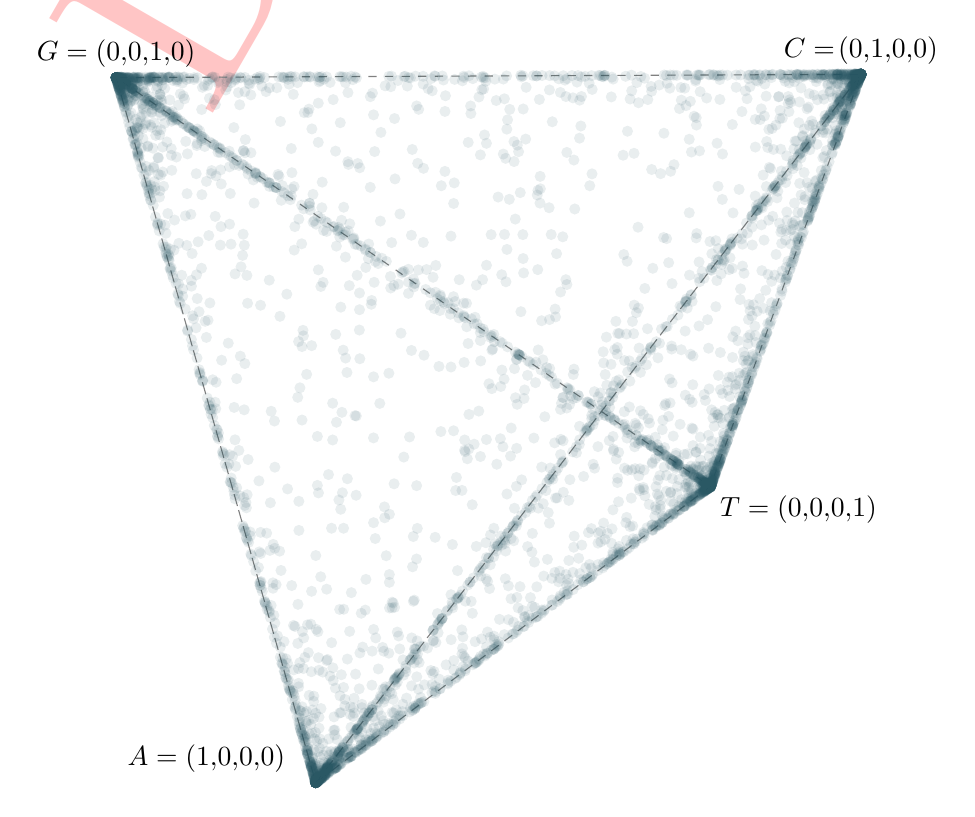
\begin{tikzpicture}[scale=10]


\begin{scope}[rotate around y=45,rotate around z=45]
 
% Draw the vertices of the tetrahedron

\coordinate (A) at (0, 0, 0);
\coordinate (C) at (1, 0, 0);
\coordinate (G) at (0.5, 0.866, 0);
\coordinate (T) at (0.5, 0.2887, 0.816);

%\foreach \p in {A,C,G,T}\fill[black] (\p) circle (0.02);

% Draw the edges of the cube
\draw[white!50!black, dashed]  (A) -- (C) -- (G) -- (A) -- (C) -- (T) -- (A) -- (T) -- (G) --  cycle;



    \pgfmathsetmacro{\alphaa}{0.1}       
       
\fill[color1,  opacity=\alphaa] (0.423,0.586,0.046) circle (.2pt);
         \fill[color1,  opacity=\alphaa] (0.984,0.027,0) circle (.2pt);
         \fill[color1,  opacity=\alphaa] (0.286,0.29,0.207) circle (.2pt);
         \fill[color1,  opacity=\alphaa] (0.842,0.106,0) circle (.2pt);
         \fill[color1,  opacity=\alphaa] (0.604,0.399,0.404) circle (.2pt);
         \fill[color1,  opacity=\alphaa] (0.093,0.02,0.057) circle (.2pt);
         \fill[color1,  opacity=\alphaa] (0,0,0) circle (.2pt);
         \fill[color1,  opacity=\alphaa] (0.231,0,0) circle (.2pt);
         \fill[color1,  opacity=\alphaa] (1,0,0) circle (.2pt);
         \fill[color1,  opacity=\alphaa] (0.36,0.556,0.003) circle (.2pt);
         \fill[color1,  opacity=\alphaa] (0.454,0.593,0.229) circle (.2pt);
         \fill[color1,  opacity=\alphaa] (0.506,0.85,0) circle (.2pt);
         \fill[color1,  opacity=\alphaa] (0.414,0.41,0.052) circle (.2pt);
         \fill[color1,  opacity=\alphaa] (0.533,0.269,0.762) circle (.2pt);
         \fill[color1,  opacity=\alphaa] (0.488,0.837,0) circle (.2pt);
         \fill[color1,  opacity=\alphaa] (0.001,0,0) circle (.2pt);
         \fill[color1,  opacity=\alphaa] (0.364,0.631,0) circle (.2pt);
         \fill[color1,  opacity=\alphaa] (0.495,0.836,0) circle (.2pt);
         \fill[color1,  opacity=\alphaa] (0.996,0.001,0) circle (.2pt);
         \fill[color1,  opacity=\alphaa] (0.999,0,0.001) circle (.2pt);
         \fill[color1,  opacity=\alphaa] (0.453,0.784,0) circle (.2pt);
         \fill[color1,  opacity=\alphaa] (0.405,0.235,0.66) circle (.2pt);
         \fill[color1,  opacity=\alphaa] (0.828,0.099,0.281) circle (.2pt);
         \fill[color1,  opacity=\alphaa] (0.648,0.186,0.526) circle (.2pt);
         \fill[color1,  opacity=\alphaa] (0.488,0.846,0) circle (.2pt);
         \fill[color1,  opacity=\alphaa] (0.47,0.438,0.499) circle (.2pt);
         \fill[color1,  opacity=\alphaa] (0.498,0.863,0) circle (.2pt);
         \fill[color1,  opacity=\alphaa] (0.006,0.01,0) circle (.2pt);
         \fill[color1,  opacity=\alphaa] (0.5,0.839,0.038) circle (.2pt);
         \fill[color1,  opacity=\alphaa] (0.605,0.051,0) circle (.2pt);
         \fill[color1,  opacity=\alphaa] (0.485,0.287,0.782) circle (.2pt);
         \fill[color1,  opacity=\alphaa] (0.516,0.502,0.418) circle (.2pt);
         \fill[color1,  opacity=\alphaa] (0.035,0.025,0.051) circle (.2pt);
         \fill[color1,  opacity=\alphaa] (0.5,0.289,0.816) circle (.2pt);
         \fill[color1,  opacity=\alphaa] (0.267,0.463,0) circle (.2pt);
         \fill[color1,  opacity=\alphaa] (0.5,0.289,0.816) circle (.2pt);
         \fill[color1,  opacity=\alphaa] (0.482,0.827,0) circle (.2pt);
         \fill[color1,  opacity=\alphaa] (0.5,0.298,0.804) circle (.2pt);
         \fill[color1,  opacity=\alphaa] (0.5,0.866,0) circle (.2pt);
         \fill[color1,  opacity=\alphaa] (0.5,0.289,0.816) circle (.2pt);
         \fill[color1,  opacity=\alphaa] (0.844,0.092,0.252) circle (.2pt);
         \fill[color1,  opacity=\alphaa] (0.476,0.583,0.341) circle (.2pt);
         \fill[color1,  opacity=\alphaa] (0.46,0.777,0.029) circle (.2pt);
         \fill[color1,  opacity=\alphaa] (0.996,0.007,0) circle (.2pt);
         \fill[color1,  opacity=\alphaa] (0.392,0.498,0.256) circle (.2pt);
         \fill[color1,  opacity=\alphaa] (0.977,0.013,0.038) circle (.2pt);
         \fill[color1,  opacity=\alphaa] (0.95,0.032,0.077) circle (.2pt);
         \fill[color1,  opacity=\alphaa] (0.436,0.611,0.002) circle (.2pt);
         \fill[color1,  opacity=\alphaa] (0.025,0.029,0.019) circle (.2pt);
         \fill[color1,  opacity=\alphaa] (0.952,0.028,0.079) circle (.2pt);
         \fill[color1,  opacity=\alphaa] (0.975,0.004,0.011) circle (.2pt);
         \fill[color1,  opacity=\alphaa] (0.006,0.002,0.006) circle (.2pt);
         \fill[color1,  opacity=\alphaa] (0.52,0.261,0.738) circle (.2pt);
         \fill[color1,  opacity=\alphaa] (0.319,0.184,0.521) circle (.2pt);
         \fill[color1,  opacity=\alphaa] (0.382,0.238,0.595) circle (.2pt);
         \fill[color1,  opacity=\alphaa] (0.207,0.357,0) circle (.2pt);
         \fill[color1,  opacity=\alphaa] (0.5,0.851,0.022) circle (.2pt);
         \fill[color1,  opacity=\alphaa] (0.575,0.22,0.616) circle (.2pt);
         \fill[color1,  opacity=\alphaa] (0.489,0.804,0.06) circle (.2pt);
         \fill[color1,  opacity=\alphaa] (0.968,0.006,0) circle (.2pt);
         \fill[color1,  opacity=\alphaa] (0.403,0,0) circle (.2pt);
         \fill[color1,  opacity=\alphaa] (0.008,0,0) circle (.2pt);
         \fill[color1,  opacity=\alphaa] (0.523,0.275,0.778) circle (.2pt);
         \fill[color1,  opacity=\alphaa] (0.5,0.474,0.554) circle (.2pt);
         \fill[color1,  opacity=\alphaa] (0.516,0.822,0.022) circle (.2pt);
         \fill[color1,  opacity=\alphaa] (0.021,0.001,0.003) circle (.2pt);
         \fill[color1,  opacity=\alphaa] (0.5,0.866,0) circle (.2pt);
         \fill[color1,  opacity=\alphaa] (0.339,0,0) circle (.2pt);
         \fill[color1,  opacity=\alphaa] (0.505,0.856,0.002) circle (.2pt);
         \fill[color1,  opacity=\alphaa] (0.002,0,0) circle (.2pt);
         \fill[color1,  opacity=\alphaa] (0.132,0.044,0.125) circle (.2pt);
         \fill[color1,  opacity=\alphaa] (0.508,0.851,0) circle (.2pt);
         \fill[color1,  opacity=\alphaa] (0,0,0) circle (.2pt);
         \fill[color1,  opacity=\alphaa] (0.831,0.29,0.003) circle (.2pt);
         \fill[color1,  opacity=\alphaa] (0,0,0) circle (.2pt);
         \fill[color1,  opacity=\alphaa] (0.502,0.301,0.793) circle (.2pt);
         \fill[color1,  opacity=\alphaa] (0.598,0.67,0.001) circle (.2pt);
         \fill[color1,  opacity=\alphaa] (0.5,0.846,0.028) circle (.2pt);
         \fill[color1,  opacity=\alphaa] (0.979,0.037,0) circle (.2pt);
         \fill[color1,  opacity=\alphaa] (0.548,0.78,0) circle (.2pt);
         \fill[color1,  opacity=\alphaa] (0.528,0.273,0.771) circle (.2pt);
         \fill[color1,  opacity=\alphaa] (0.445,0.769,0) circle (.2pt);
         \fill[color1,  opacity=\alphaa] (1,0,0) circle (.2pt);
         \fill[color1,  opacity=\alphaa] (0.461,0.264,0.748) circle (.2pt);
         \fill[color1,  opacity=\alphaa] (0.486,0.779,0.087) circle (.2pt);
         \fill[color1,  opacity=\alphaa] (0.074,0.018,0.034) circle (.2pt);
         \fill[color1,  opacity=\alphaa] (0.205,0.014,0.04) circle (.2pt);
         \fill[color1,  opacity=\alphaa] (0.501,0.288,0.815) circle (.2pt);
         \fill[color1,  opacity=\alphaa] (0.901,0.171,0) circle (.2pt);
         \fill[color1,  opacity=\alphaa] (0.5,0.305,0.793) circle (.2pt);
         \fill[color1,  opacity=\alphaa] (0.476,0.275,0.777) circle (.2pt);
         \fill[color1,  opacity=\alphaa] (0.563,0.749,0.011) circle (.2pt);
         \fill[color1,  opacity=\alphaa] (0.194,0.005,0.014) circle (.2pt);
         \fill[color1,  opacity=\alphaa] (0.5,0.289,0.816) circle (.2pt);
         \fill[color1,  opacity=\alphaa] (0.984,0,0) circle (.2pt);
         \fill[color1,  opacity=\alphaa] (0.97,0.016,0.013) circle (.2pt);
         \fill[color1,  opacity=\alphaa] (0.494,0.855,0) circle (.2pt);
         \fill[color1,  opacity=\alphaa] (0.497,0.287,0.811) circle (.2pt);
         \fill[color1,  opacity=\alphaa] (0.883,0.202,0) circle (.2pt);
         \fill[color1,  opacity=\alphaa] (0.305,0.055,0.001) circle (.2pt);
         \fill[color1,  opacity=\alphaa] (0.356,0.211,0.574) circle (.2pt);
         \fill[color1,  opacity=\alphaa] (0.02,0.035,0) circle (.2pt);
         \fill[color1,  opacity=\alphaa] (0.796,0.117,0.33) circle (.2pt);
         \fill[color1,  opacity=\alphaa] (0.391,0.161,0.43) circle (.2pt);
         \fill[color1,  opacity=\alphaa] (0.099,0.001,0) circle (.2pt);
         \fill[color1,  opacity=\alphaa] (0,0,0) circle (.2pt);
         \fill[color1,  opacity=\alphaa] (0.483,0.411,0.603) circle (.2pt);
         \fill[color1,  opacity=\alphaa] (0.5,0.289,0.816) circle (.2pt);
         \fill[color1,  opacity=\alphaa] (0.499,0.288,0.815) circle (.2pt);
         \fill[color1,  opacity=\alphaa] (0.499,0.864,0) circle (.2pt);
         \fill[color1,  opacity=\alphaa] (0.496,0.285,0.807) circle (.2pt);
         \fill[color1,  opacity=\alphaa] (0.493,0.852,0.002) circle (.2pt);
         \fill[color1,  opacity=\alphaa] (0.501,0.296,0.803) circle (.2pt);
         \fill[color1,  opacity=\alphaa] (0.155,0.26,0) circle (.2pt);
         \fill[color1,  opacity=\alphaa] (0.493,0.285,0.806) circle (.2pt);
         \fill[color1,  opacity=\alphaa] (0.581,0.14,0.377) circle (.2pt);
         \fill[color1,  opacity=\alphaa] (0.738,0,0) circle (.2pt);
         \fill[color1,  opacity=\alphaa] (0.655,0.199,0.563) circle (.2pt);
         \fill[color1,  opacity=\alphaa] (0.492,0.694,0.221) circle (.2pt);
         \fill[color1,  opacity=\alphaa] (0.502,0.86,0.004) circle (.2pt);
         \fill[color1,  opacity=\alphaa] (0.725,0.023,0.066) circle (.2pt);
         \fill[color1,  opacity=\alphaa] (0.029,0.049,0) circle (.2pt);
         \fill[color1,  opacity=\alphaa] (0.262,0,0) circle (.2pt);
         \fill[color1,  opacity=\alphaa] (0.382,0.368,0.414) circle (.2pt);
         \fill[color1,  opacity=\alphaa] (0.999,0.001,0.002) circle (.2pt);
         \fill[color1,  opacity=\alphaa] (0.5,0.313,0.783) circle (.2pt);
         \fill[color1,  opacity=\alphaa] (0.999,0,0) circle (.2pt);
         \fill[color1,  opacity=\alphaa] (0.496,0.858,0.001) circle (.2pt);
         \fill[color1,  opacity=\alphaa] (0.71,0.171,0.469) circle (.2pt);
         \fill[color1,  opacity=\alphaa] (0.025,0.014,0.041) circle (.2pt);
         \fill[color1,  opacity=\alphaa] (0.049,0,0) circle (.2pt);
         \fill[color1,  opacity=\alphaa] (0.439,0.15,0.424) circle (.2pt);
         \fill[color1,  opacity=\alphaa] (0.261,0.151,0.418) circle (.2pt);
         \fill[color1,  opacity=\alphaa] (0,0,0) circle (.2pt);
         \fill[color1,  opacity=\alphaa] (0.5,0.864,0.002) circle (.2pt);
         \fill[color1,  opacity=\alphaa] (0.347,0.427,0.242) circle (.2pt);
         \fill[color1,  opacity=\alphaa] (0.95,0.029,0.081) circle (.2pt);
         \fill[color1,  opacity=\alphaa] (1,0,0) circle (.2pt);
         \fill[color1,  opacity=\alphaa] (0.988,0.02,0) circle (.2pt);
         \fill[color1,  opacity=\alphaa] (0.784,0.124,0.35) circle (.2pt);
         \fill[color1,  opacity=\alphaa] (0.468,0.274,0.759) circle (.2pt);
         \fill[color1,  opacity=\alphaa] (0.286,0.093,0.263) circle (.2pt);
         \fill[color1,  opacity=\alphaa] (0.493,0.847,0.009) circle (.2pt);
         \fill[color1,  opacity=\alphaa] (0.927,0,0) circle (.2pt);
         \fill[color1,  opacity=\alphaa] (0.429,0,0) circle (.2pt);
         \fill[color1,  opacity=\alphaa] (0.916,0.047,0.133) circle (.2pt);
         \fill[color1,  opacity=\alphaa] (0.613,0,0.001) circle (.2pt);
         \fill[color1,  opacity=\alphaa] (0.5,0.327,0.763) circle (.2pt);
         \fill[color1,  opacity=\alphaa] (0.963,0.007,0) circle (.2pt);
         \fill[color1,  opacity=\alphaa] (0.534,0.268,0.759) circle (.2pt);
         \fill[color1,  opacity=\alphaa] (0.483,0.309,0.747) circle (.2pt);
         \fill[color1,  opacity=\alphaa] (0.499,0.865,0) circle (.2pt);
         \fill[color1,  opacity=\alphaa] (0.285,0.452,0.057) circle (.2pt);
         \fill[color1,  opacity=\alphaa] (0.848,0.088,0.247) circle (.2pt);
         \fill[color1,  opacity=\alphaa] (0.118,0.203,0.003) circle (.2pt);
         \fill[color1,  opacity=\alphaa] (1,0,0) circle (.2pt);
         \fill[color1,  opacity=\alphaa] (0.261,0.018,0.05) circle (.2pt);
         \fill[color1,  opacity=\alphaa] (0.5,0.866,0) circle (.2pt);
         \fill[color1,  opacity=\alphaa] (0.5,0.339,0.744) circle (.2pt);
         \fill[color1,  opacity=\alphaa] (0.066,0.113,0) circle (.2pt);
         \fill[color1,  opacity=\alphaa] (0.507,0.285,0.806) circle (.2pt);
         \fill[color1,  opacity=\alphaa] (0.023,0.004,0.01) circle (.2pt);
         \fill[color1,  opacity=\alphaa] (0.139,0.148,0) circle (.2pt);
         \fill[color1,  opacity=\alphaa] (0.507,0.332,0.74) circle (.2pt);
         \fill[color1,  opacity=\alphaa] (0.5,0.865,0.001) circle (.2pt);
         \fill[color1,  opacity=\alphaa] (0.5,0.301,0.799) circle (.2pt);
         \fill[color1,  opacity=\alphaa] (0.012,0.021,0) circle (.2pt);
         \fill[color1,  opacity=\alphaa] (0.459,0.767,0) circle (.2pt);
         \fill[color1,  opacity=\alphaa] (0.779,0.128,0.36) circle (.2pt);
         \fill[color1,  opacity=\alphaa] (0.5,0.699,0.236) circle (.2pt);
         \fill[color1,  opacity=\alphaa] (0.868,0.229,0) circle (.2pt);
         \fill[color1,  opacity=\alphaa] (0.004,0,0) circle (.2pt);
         \fill[color1,  opacity=\alphaa] (0.5,0.663,0.288) circle (.2pt);
         \fill[color1,  opacity=\alphaa] (0.496,0.507,0.498) circle (.2pt);
         \fill[color1,  opacity=\alphaa] (0.184,0.289,0.043) circle (.2pt);
         \fill[color1,  opacity=\alphaa] (0.5,0.863,0.004) circle (.2pt);
         \fill[color1,  opacity=\alphaa] (0.955,0.032,0.066) circle (.2pt);
         \fill[color1,  opacity=\alphaa] (0.484,0.838,0.002) circle (.2pt);
         \fill[color1,  opacity=\alphaa] (0.043,0.074,0) circle (.2pt);
         \fill[color1,  opacity=\alphaa] (0.501,0.31,0.784) circle (.2pt);
         \fill[color1,  opacity=\alphaa] (0.992,0.009,0) circle (.2pt);
         \fill[color1,  opacity=\alphaa] (0.491,0.851,0) circle (.2pt);
         \fill[color1,  opacity=\alphaa] (0.499,0.291,0.809) circle (.2pt);
         \fill[color1,  opacity=\alphaa] (0,0,0) circle (.2pt);
         \fill[color1,  opacity=\alphaa] (0.047,0.012,0.033) circle (.2pt);
         \fill[color1,  opacity=\alphaa] (0.961,0.067,0) circle (.2pt);
         \fill[color1,  opacity=\alphaa] (0.502,0.287,0.813) circle (.2pt);
         \fill[color1,  opacity=\alphaa] (0.499,0.288,0.814) circle (.2pt);
         \fill[color1,  opacity=\alphaa] (0.181,0.161,0) circle (.2pt);
         \fill[color1,  opacity=\alphaa] (0.455,0.783,0.001) circle (.2pt);
         \fill[color1,  opacity=\alphaa] (0.875,0,0) circle (.2pt);
         \fill[color1,  opacity=\alphaa] (0.505,0.304,0.782) circle (.2pt);
         \fill[color1,  opacity=\alphaa] (0.66,0.221,0.519) circle (.2pt);
         \fill[color1,  opacity=\alphaa] (0.564,0.252,0.712) circle (.2pt);
         \fill[color1,  opacity=\alphaa] (0.5,0.289,0.816) circle (.2pt);
         \fill[color1,  opacity=\alphaa] (0.5,0.289,0.816) circle (.2pt);
         \fill[color1,  opacity=\alphaa] (0.667,0.325,0.355) circle (.2pt);
         \fill[color1,  opacity=\alphaa] (1,0,0) circle (.2pt);
         \fill[color1,  opacity=\alphaa] (0.406,0.454,0.29) circle (.2pt);
         \fill[color1,  opacity=\alphaa] (0.55,0.776,0.004) circle (.2pt);
         \fill[color1,  opacity=\alphaa] (0.309,0.179,0.505) circle (.2pt);
         \fill[color1,  opacity=\alphaa] (0.5,0.861,0.007) circle (.2pt);
         \fill[color1,  opacity=\alphaa] (0.47,0.723,0.127) circle (.2pt);
         \fill[color1,  opacity=\alphaa] (0.061,0.03,0.083) circle (.2pt);
         \fill[color1,  opacity=\alphaa] (1,0,0) circle (.2pt);
         \fill[color1,  opacity=\alphaa] (0.5,0.288,0.816) circle (.2pt);
         \fill[color1,  opacity=\alphaa] (0.001,0,0) circle (.2pt);
         \fill[color1,  opacity=\alphaa] (0.5,0.865,0) circle (.2pt);
         \fill[color1,  opacity=\alphaa] (0.883,0.203,0) circle (.2pt);
         \fill[color1,  opacity=\alphaa] (0.224,0,0) circle (.2pt);
         \fill[color1,  opacity=\alphaa] (0.849,0.234,0) circle (.2pt);
         \fill[color1,  opacity=\alphaa] (0.484,0,0) circle (.2pt);
         \fill[color1,  opacity=\alphaa] (0.732,0.154,0.437) circle (.2pt);
         \fill[color1,  opacity=\alphaa] (0.998,0.001,0.004) circle (.2pt);
         \fill[color1,  opacity=\alphaa] (0.46,0.424,0.526) circle (.2pt);
         \fill[color1,  opacity=\alphaa] (0.524,0.825,0) circle (.2pt);
         \fill[color1,  opacity=\alphaa] (0.531,0.026,0.054) circle (.2pt);
         \fill[color1,  opacity=\alphaa] (0.022,0.001,0) circle (.2pt);
         \fill[color1,  opacity=\alphaa] (0.733,0.037,0.099) circle (.2pt);
         \fill[color1,  opacity=\alphaa] (0.5,0.339,0.745) circle (.2pt);
         \fill[color1,  opacity=\alphaa] (0.993,0.013,0) circle (.2pt);
         \fill[color1,  opacity=\alphaa] (0.5,0.857,0.013) circle (.2pt);
         \fill[color1,  opacity=\alphaa] (0.995,0.001,0.001) circle (.2pt);
         \fill[color1,  opacity=\alphaa] (0.075,0.103,0.039) circle (.2pt);
         \fill[color1,  opacity=\alphaa] (0.994,0.003,0.009) circle (.2pt);
         \fill[color1,  opacity=\alphaa] (0.855,0.021,0) circle (.2pt);
         \fill[color1,  opacity=\alphaa] (0.5,0.856,0.014) circle (.2pt);
         \fill[color1,  opacity=\alphaa] (0.995,0.003,0.008) circle (.2pt);
         \fill[color1,  opacity=\alphaa] (1,0,0) circle (.2pt);
         \fill[color1,  opacity=\alphaa] (0.002,0.001,0) circle (.2pt);
         \fill[color1,  opacity=\alphaa] (0.994,0,0.001) circle (.2pt);
         \fill[color1,  opacity=\alphaa] (0.493,0.281,0.794) circle (.2pt);
         \fill[color1,  opacity=\alphaa] (0.825,0.303,0) circle (.2pt);
         \fill[color1,  opacity=\alphaa] (0.501,0.859,0.008) circle (.2pt);
         \fill[color1,  opacity=\alphaa] (0.496,0.286,0.808) circle (.2pt);
         \fill[color1,  opacity=\alphaa] (0.497,0.283,0.799) circle (.2pt);
         \fill[color1,  opacity=\alphaa] (0.501,0.288,0.814) circle (.2pt);
         \fill[color1,  opacity=\alphaa] (0.502,0.298,0.798) circle (.2pt);
         \fill[color1,  opacity=\alphaa] (0.229,0.059,0.017) circle (.2pt);
         \fill[color1,  opacity=\alphaa] (0.5,0.858,0.011) circle (.2pt);
         \fill[color1,  opacity=\alphaa] (0.5,0.866,0) circle (.2pt);
         \fill[color1,  opacity=\alphaa] (0.17,0.06,0) circle (.2pt);
         \fill[color1,  opacity=\alphaa] (0.398,0.686,0.006) circle (.2pt);
         \fill[color1,  opacity=\alphaa] (0.949,0.071,0) circle (.2pt);
         \fill[color1,  opacity=\alphaa] (0.5,0.289,0.816) circle (.2pt);
         \fill[color1,  opacity=\alphaa] (0.976,0.03,0) circle (.2pt);
         \fill[color1,  opacity=\alphaa] (0.286,0.109,0.003) circle (.2pt);
         \fill[color1,  opacity=\alphaa] (0.002,0.001,0.002) circle (.2pt);
         \fill[color1,  opacity=\alphaa] (0.345,0.559,0) circle (.2pt);
         \fill[color1,  opacity=\alphaa] (0.456,0.633,0.219) circle (.2pt);
         \fill[color1,  opacity=\alphaa] (0.499,0.833,0.045) circle (.2pt);
         \fill[color1,  opacity=\alphaa] (0.01,0.005,0.002) circle (.2pt);
         \fill[color1,  opacity=\alphaa] (0.491,0.33,0.735) circle (.2pt);
         \fill[color1,  opacity=\alphaa] (0.554,0.752,0) circle (.2pt);
         \fill[color1,  opacity=\alphaa] (0.493,0.854,0) circle (.2pt);
         \fill[color1,  opacity=\alphaa] (0.999,0.001,0) circle (.2pt);
         \fill[color1,  opacity=\alphaa] (0.984,0.028,0) circle (.2pt);
         \fill[color1,  opacity=\alphaa] (0.999,0,0) circle (.2pt);
         \fill[color1,  opacity=\alphaa] (0.071,0.041,0.117) circle (.2pt);
         \fill[color1,  opacity=\alphaa] (0,0,0) circle (.2pt);
         \fill[color1,  opacity=\alphaa] (0.572,0.649,0.13) circle (.2pt);
         \fill[color1,  opacity=\alphaa] (0.406,0.235,0.662) circle (.2pt);
         \fill[color1,  opacity=\alphaa] (0.001,0.001,0.001) circle (.2pt);
         \fill[color1,  opacity=\alphaa] (0.998,0.001,0.003) circle (.2pt);
         \fill[color1,  opacity=\alphaa] (0.334,0,0) circle (.2pt);
         \fill[color1,  opacity=\alphaa] (0.989,0,0) circle (.2pt);
         \fill[color1,  opacity=\alphaa] (0.716,0.485,0.005) circle (.2pt);
         \fill[color1,  opacity=\alphaa] (0.002,0.004,0) circle (.2pt);
         \fill[color1,  opacity=\alphaa] (0.948,0.033,0.08) circle (.2pt);
         \fill[color1,  opacity=\alphaa] (0.996,0.002,0.007) circle (.2pt);
         \fill[color1,  opacity=\alphaa] (0.03,0.048,0) circle (.2pt);
         \fill[color1,  opacity=\alphaa] (0.503,0.335,0.744) circle (.2pt);
         \fill[color1,  opacity=\alphaa] (0.241,0.001,0) circle (.2pt);
         \fill[color1,  opacity=\alphaa] (0.063,0,0) circle (.2pt);
         \fill[color1,  opacity=\alphaa] (0.5,0.289,0.816) circle (.2pt);
         \fill[color1,  opacity=\alphaa] (0,0,0) circle (.2pt);
         \fill[color1,  opacity=\alphaa] (0.026,0,0) circle (.2pt);
         \fill[color1,  opacity=\alphaa] (0.021,0.037,0) circle (.2pt);
         \fill[color1,  opacity=\alphaa] (0.511,0.836,0.013) circle (.2pt);
         \fill[color1,  opacity=\alphaa] (0.953,0.027,0.076) circle (.2pt);
         \fill[color1,  opacity=\alphaa] (0.013,0,0) circle (.2pt);
         \fill[color1,  opacity=\alphaa] (0.452,0.288,0.7) circle (.2pt);
         \fill[color1,  opacity=\alphaa] (0.004,0.002,0.006) circle (.2pt);
         \fill[color1,  opacity=\alphaa] (0.455,0.055,0) circle (.2pt);
         \fill[color1,  opacity=\alphaa] (0.775,0.13,0.367) circle (.2pt);
         \fill[color1,  opacity=\alphaa] (0.5,0.289,0.816) circle (.2pt);
         \fill[color1,  opacity=\alphaa] (0.841,0,0) circle (.2pt);
         \fill[color1,  opacity=\alphaa] (0.732,0.004,0.009) circle (.2pt);
         \fill[color1,  opacity=\alphaa] (0.488,0.282,0.797) circle (.2pt);
         \fill[color1,  opacity=\alphaa] (0.003,0.005,0) circle (.2pt);
         \fill[color1,  opacity=\alphaa] (0.5,0.866,0.001) circle (.2pt);
         \fill[color1,  opacity=\alphaa] (0.513,0.281,0.796) circle (.2pt);
         \fill[color1,  opacity=\alphaa] (0.497,0.31,0.778) circle (.2pt);
         \fill[color1,  opacity=\alphaa] (0.83,0.289,0.007) circle (.2pt);
         \fill[color1,  opacity=\alphaa] (0.501,0.288,0.814) circle (.2pt);
         \fill[color1,  opacity=\alphaa] (0.5,0.29,0.815) circle (.2pt);
         \fill[color1,  opacity=\alphaa] (0.971,0.02,0.041) circle (.2pt);
         \fill[color1,  opacity=\alphaa] (0,0,0) circle (.2pt);
         \fill[color1,  opacity=\alphaa] (0.513,0.82,0.034) circle (.2pt);
         \fill[color1,  opacity=\alphaa] (0.518,0.67,0.234) circle (.2pt);
         \fill[color1,  opacity=\alphaa] (0.989,0.006,0.018) circle (.2pt);
         \fill[color1,  opacity=\alphaa] (1,0,0) circle (.2pt);
         \fill[color1,  opacity=\alphaa] (0.5,0.854,0.017) circle (.2pt);
         \fill[color1,  opacity=\alphaa] (0.501,0.797,0.059) circle (.2pt);
         \fill[color1,  opacity=\alphaa] (0.783,0.139,0.335) circle (.2pt);
         \fill[color1,  opacity=\alphaa] (0.194,0.135,0.01) circle (.2pt);
         \fill[color1,  opacity=\alphaa] (0.504,0.86,0) circle (.2pt);
         \fill[color1,  opacity=\alphaa] (0.915,0.049,0.139) circle (.2pt);
         \fill[color1,  opacity=\alphaa] (0.006,0.003,0.01) circle (.2pt);
         \fill[color1,  opacity=\alphaa] (0.5,0.393,0.669) circle (.2pt);
         \fill[color1,  opacity=\alphaa] (0.001,0,0.001) circle (.2pt);
         \fill[color1,  opacity=\alphaa] (0.916,0.089,0.065) circle (.2pt);
         \fill[color1,  opacity=\alphaa] (0.003,0,0) circle (.2pt);
         \fill[color1,  opacity=\alphaa] (0.552,0.216,0.612) circle (.2pt);
         \fill[color1,  opacity=\alphaa] (0.987,0.023,0) circle (.2pt);
         \fill[color1,  opacity=\alphaa] (0.883,0,0) circle (.2pt);
         \fill[color1,  opacity=\alphaa] (0.362,0,0) circle (.2pt);
         \fill[color1,  opacity=\alphaa] (0.952,0.003,0.003) circle (.2pt);
         \fill[color1,  opacity=\alphaa] (0.091,0.151,0.009) circle (.2pt);
         \fill[color1,  opacity=\alphaa] (0.426,0.733,0.007) circle (.2pt);
         \fill[color1,  opacity=\alphaa] (0.5,0.861,0.007) circle (.2pt);
         \fill[color1,  opacity=\alphaa] (0.5,0.289,0.816) circle (.2pt);
         \fill[color1,  opacity=\alphaa] (0.62,0.658,0) circle (.2pt);
         \fill[color1,  opacity=\alphaa] (0.785,0.341,0.044) circle (.2pt);
         \fill[color1,  opacity=\alphaa] (0.004,0.007,0) circle (.2pt);
         \fill[color1,  opacity=\alphaa] (0.702,0.185,0.416) circle (.2pt);
         \fill[color1,  opacity=\alphaa] (0.071,0.041,0.116) circle (.2pt);
         \fill[color1,  opacity=\alphaa] (0.498,0.311,0.781) circle (.2pt);
         \fill[color1,  opacity=\alphaa] (0.499,0.86,0.006) circle (.2pt);
         \fill[color1,  opacity=\alphaa] (0.508,0.85,0) circle (.2pt);
         \fill[color1,  opacity=\alphaa] (0.006,0,0) circle (.2pt);
         \fill[color1,  opacity=\alphaa] (0.523,0.826,0) circle (.2pt);
         \fill[color1,  opacity=\alphaa] (0.001,0,0) circle (.2pt);
         \fill[color1,  opacity=\alphaa] (0.49,0.087,0.243) circle (.2pt);
         \fill[color1,  opacity=\alphaa] (0.5,0.857,0.013) circle (.2pt);
         \fill[color1,  opacity=\alphaa] (0.5,0.771,0.134) circle (.2pt);
         \fill[color1,  opacity=\alphaa] (0.444,0.365,0.572) circle (.2pt);
         \fill[color1,  opacity=\alphaa] (0.313,0.175,0.494) circle (.2pt);
         \fill[color1,  opacity=\alphaa] (0.497,0.287,0.812) circle (.2pt);
         \fill[color1,  opacity=\alphaa] (0.167,0.096,0.273) circle (.2pt);
         \fill[color1,  opacity=\alphaa] (0.5,0.528,0.477) circle (.2pt);
         \fill[color1,  opacity=\alphaa] (0.473,0.791,0.039) circle (.2pt);
         \fill[color1,  opacity=\alphaa] (0.892,0.187,0) circle (.2pt);
         \fill[color1,  opacity=\alphaa] (0.187,0.003,0) circle (.2pt);
         \fill[color1,  opacity=\alphaa] (0.497,0.857,0) circle (.2pt);
         \fill[color1,  opacity=\alphaa] (1,0,0) circle (.2pt);
         \fill[color1,  opacity=\alphaa] (0.031,0.018,0.051) circle (.2pt);
         \fill[color1,  opacity=\alphaa] (0.495,0.857,0) circle (.2pt);
         \fill[color1,  opacity=\alphaa] (0.807,0.3,0) circle (.2pt);
         \fill[color1,  opacity=\alphaa] (0.226,0.131,0.37) circle (.2pt);
         \fill[color1,  opacity=\alphaa] (0.984,0,0) circle (.2pt);
         \fill[color1,  opacity=\alphaa] (0.498,0.288,0.813) circle (.2pt);
         \fill[color1,  opacity=\alphaa] (0.011,0.019,0) circle (.2pt);
         \fill[color1,  opacity=\alphaa] (0.5,0.289,0.816) circle (.2pt);
         \fill[color1,  opacity=\alphaa] (0.936,0.11,0) circle (.2pt);
         \fill[color1,  opacity=\alphaa] (0.491,0.283,0.801) circle (.2pt);
         \fill[color1,  opacity=\alphaa] (0.419,0.242,0.675) circle (.2pt);
         \fill[color1,  opacity=\alphaa] (0.538,0.267,0.754) circle (.2pt);
         \fill[color1,  opacity=\alphaa] (0.501,0.288,0.814) circle (.2pt);
         \fill[color1,  opacity=\alphaa] (0.5,0.355,0.722) circle (.2pt);
         \fill[color1,  opacity=\alphaa] (0,0.001,0) circle (.2pt);
         \fill[color1,  opacity=\alphaa] (0.286,0.165,0.467) circle (.2pt);
         \fill[color1,  opacity=\alphaa] (0.5,0.67,0.277) circle (.2pt);
         \fill[color1,  opacity=\alphaa] (0.03,0,0) circle (.2pt);
         \fill[color1,  opacity=\alphaa] (0.072,0.035,0.099) circle (.2pt);
         \fill[color1,  opacity=\alphaa] (0.491,0.283,0.8) circle (.2pt);
         \fill[color1,  opacity=\alphaa] (0.113,0.146,0) circle (.2pt);
         \fill[color1,  opacity=\alphaa] (0.5,0.445,0.594) circle (.2pt);
         \fill[color1,  opacity=\alphaa] (0.246,0.426,0) circle (.2pt);
         \fill[color1,  opacity=\alphaa] (0.528,0.219,0.618) circle (.2pt);
         \fill[color1,  opacity=\alphaa] (0.985,0.012,0.021) circle (.2pt);
         \fill[color1,  opacity=\alphaa] (0.503,0.291,0.803) circle (.2pt);
         \fill[color1,  opacity=\alphaa] (0.5,0.85,0.023) circle (.2pt);
         \fill[color1,  opacity=\alphaa] (0.201,0.339,0.012) circle (.2pt);
         \fill[color1,  opacity=\alphaa] (0.5,0.766,0.141) circle (.2pt);
         \fill[color1,  opacity=\alphaa] (0.069,0.075,0.063) circle (.2pt);
         \fill[color1,  opacity=\alphaa] (0.999,0,0.001) circle (.2pt);
         \fill[color1,  opacity=\alphaa] (0.722,0.161,0.454) circle (.2pt);
         \fill[color1,  opacity=\alphaa] (0.501,0.3,0.798) circle (.2pt);
         \fill[color1,  opacity=\alphaa] (0.264,0.153,0.432) circle (.2pt);
         \fill[color1,  opacity=\alphaa] (0.077,0,0) circle (.2pt);
         \fill[color1,  opacity=\alphaa] (0.812,0.088,0.239) circle (.2pt);
         \fill[color1,  opacity=\alphaa] (0.565,0.488,0.376) circle (.2pt);
         \fill[color1,  opacity=\alphaa] (0.968,0.055,0) circle (.2pt);
         \fill[color1,  opacity=\alphaa] (0,0,0.001) circle (.2pt);
         \fill[color1,  opacity=\alphaa] (0.526,0.822,0) circle (.2pt);
         \fill[color1,  opacity=\alphaa] (0.467,0.27,0.762) circle (.2pt);
         \fill[color1,  opacity=\alphaa] (0.025,0,0) circle (.2pt);
         \fill[color1,  opacity=\alphaa] (0.5,0.325,0.765) circle (.2pt);
         \fill[color1,  opacity=\alphaa] (0.257,0.301,0.143) circle (.2pt);
         \fill[color1,  opacity=\alphaa] (0.009,0,0.001) circle (.2pt);
         \fill[color1,  opacity=\alphaa] (0.686,0.53,0.019) circle (.2pt);
         \fill[color1,  opacity=\alphaa] (0.5,0.866,0) circle (.2pt);
         \fill[color1,  opacity=\alphaa] (0.735,0.191,0.38) circle (.2pt);
         \fill[color1,  opacity=\alphaa] (0.499,0.864,0) circle (.2pt);
         \fill[color1,  opacity=\alphaa] (0,0,0) circle (.2pt);
         \fill[color1,  opacity=\alphaa] (0.971,0.051,0) circle (.2pt);
         \fill[color1,  opacity=\alphaa] (0.934,0.047,0) circle (.2pt);
         \fill[color1,  opacity=\alphaa] (0.5,0.501,0.517) circle (.2pt);
         \fill[color1,  opacity=\alphaa] (0.125,0.189,0.037) circle (.2pt);
         \fill[color1,  opacity=\alphaa] (0.5,0.861,0.006) circle (.2pt);
         \fill[color1,  opacity=\alphaa] (0.5,0.788,0.109) circle (.2pt);
         \fill[color1,  opacity=\alphaa] (0.003,0.003,0.002) circle (.2pt);
         \fill[color1,  opacity=\alphaa] (0.501,0.865,0) circle (.2pt);
         \fill[color1,  opacity=\alphaa] (0.931,0.072,0.012) circle (.2pt);
         \fill[color1,  opacity=\alphaa] (0.5,0.865,0) circle (.2pt);
         \fill[color1,  opacity=\alphaa] (1,0.001,0) circle (.2pt);
         \fill[color1,  opacity=\alphaa] (0.004,0.007,0) circle (.2pt);
         \fill[color1,  opacity=\alphaa] (0.237,0.395,0) circle (.2pt);
         \fill[color1,  opacity=\alphaa] (0.499,0.294,0.807) circle (.2pt);
         \fill[color1,  opacity=\alphaa] (0.516,0.28,0.791) circle (.2pt);
         \fill[color1,  opacity=\alphaa] (0.461,0.172,0.486) circle (.2pt);
         \fill[color1,  opacity=\alphaa] (0.454,0.262,0.741) circle (.2pt);
         \fill[color1,  opacity=\alphaa] (0.013,0,0) circle (.2pt);
         \fill[color1,  opacity=\alphaa] (0.409,0.238,0.665) circle (.2pt);
         \fill[color1,  opacity=\alphaa] (0.5,0.866,0) circle (.2pt);
         \fill[color1,  opacity=\alphaa] (0.485,0.363,0.674) circle (.2pt);
         \fill[color1,  opacity=\alphaa] (0.489,0.417,0.608) circle (.2pt);
         \fill[color1,  opacity=\alphaa] (1,0,0) circle (.2pt);
         \fill[color1,  opacity=\alphaa] (0.001,0.001,0) circle (.2pt);
         \fill[color1,  opacity=\alphaa] (0.497,0.287,0.812) circle (.2pt);
         \fill[color1,  opacity=\alphaa] (0.037,0.005,0.014) circle (.2pt);
         \fill[color1,  opacity=\alphaa] (0.85,0.084,0.237) circle (.2pt);
         \fill[color1,  opacity=\alphaa] (0.46,0.537,0.286) circle (.2pt);
         \fill[color1,  opacity=\alphaa] (0.5,0.289,0.816) circle (.2pt);
         \fill[color1,  opacity=\alphaa] (0.5,0.289,0.816) circle (.2pt);
         \fill[color1,  opacity=\alphaa] (0.488,0.843,0.003) circle (.2pt);
         \fill[color1,  opacity=\alphaa] (0.482,0.278,0.783) circle (.2pt);
         \fill[color1,  opacity=\alphaa] (0.54,0.318,0.677) circle (.2pt);
         \fill[color1,  opacity=\alphaa] (0.5,0.289,0.816) circle (.2pt);
         \fill[color1,  opacity=\alphaa] (0.491,0.808,0) circle (.2pt);
         \fill[color1,  opacity=\alphaa] (0.727,0,0) circle (.2pt);
         \fill[color1,  opacity=\alphaa] (0,0,0) circle (.2pt);
         \fill[color1,  opacity=\alphaa] (0.699,0.174,0.491) circle (.2pt);
         \fill[color1,  opacity=\alphaa] (0,0,0) circle (.2pt);
         \fill[color1,  opacity=\alphaa] (0.5,0.865,0.001) circle (.2pt);
         \fill[color1,  opacity=\alphaa] (0.996,0.006,0.001) circle (.2pt);
         \fill[color1,  opacity=\alphaa] (0.901,0.172,0) circle (.2pt);
         \fill[color1,  opacity=\alphaa] (0.466,0.64,0.236) circle (.2pt);
         \fill[color1,  opacity=\alphaa] (0.062,0.034,0.094) circle (.2pt);
         \fill[color1,  opacity=\alphaa] (0.986,0.023,0) circle (.2pt);
         \fill[color1,  opacity=\alphaa] (0.997,0.002,0.005) circle (.2pt);
         \fill[color1,  opacity=\alphaa] (0.499,0.288,0.814) circle (.2pt);
         \fill[color1,  opacity=\alphaa] (0.963,0,0) circle (.2pt);
         \fill[color1,  opacity=\alphaa] (0,0,0) circle (.2pt);
         \fill[color1,  opacity=\alphaa] (0.354,0.339,0.387) circle (.2pt);
         \fill[color1,  opacity=\alphaa] (0.471,0.372,0.628) circle (.2pt);
         \fill[color1,  opacity=\alphaa] (0.971,0.017,0.046) circle (.2pt);
         \fill[color1,  opacity=\alphaa] (0.49,0.281,0.795) circle (.2pt);
         \fill[color1,  opacity=\alphaa] (0.583,0.722,0.001) circle (.2pt);
         \fill[color1,  opacity=\alphaa] (0.487,0.844,0) circle (.2pt);
         \fill[color1,  opacity=\alphaa] (0.129,0.217,0.01) circle (.2pt);
         \fill[color1,  opacity=\alphaa] (0.998,0,0) circle (.2pt);
         \fill[color1,  opacity=\alphaa] (0.504,0.86,0) circle (.2pt);
         \fill[color1,  opacity=\alphaa] (0,0,0) circle (.2pt);
         \fill[color1,  opacity=\alphaa] (0.5,0.289,0.816) circle (.2pt);
         \fill[color1,  opacity=\alphaa] (0.896,0.002,0.005) circle (.2pt);
         \fill[color1,  opacity=\alphaa] (0.961,0.066,0.002) circle (.2pt);
         \fill[color1,  opacity=\alphaa] (0.554,0.313,0.651) circle (.2pt);
         \fill[color1,  opacity=\alphaa] (0.502,0.861,0) circle (.2pt);
         \fill[color1,  opacity=\alphaa] (0.587,0.278,0.609) circle (.2pt);
         \fill[color1,  opacity=\alphaa] (0.487,0.819,0.033) circle (.2pt);
         \fill[color1,  opacity=\alphaa] (0.457,0.791,0) circle (.2pt);
         \fill[color1,  opacity=\alphaa] (0.5,0.425,0.623) circle (.2pt);
         \fill[color1,  opacity=\alphaa] (0.426,0.235,0.663) circle (.2pt);
         \fill[color1,  opacity=\alphaa] (0.511,0,0) circle (.2pt);
         \fill[color1,  opacity=\alphaa] (0.023,0,0) circle (.2pt);
         \fill[color1,  opacity=\alphaa] (0.518,0.829,0.009) circle (.2pt);
         \fill[color1,  opacity=\alphaa] (0.877,0.002,0) circle (.2pt);
         \fill[color1,  opacity=\alphaa] (0.604,0.228,0.646) circle (.2pt);
         \fill[color1,  opacity=\alphaa] (0.027,0.042,0) circle (.2pt);
         \fill[color1,  opacity=\alphaa] (0.976,0.039,0) circle (.2pt);
         \fill[color1,  opacity=\alphaa] (0.497,0.291,0.806) circle (.2pt);
         \fill[color1,  opacity=\alphaa] (0.496,0.571,0.406) circle (.2pt);
         \fill[color1,  opacity=\alphaa] (0.558,0.371,0.385) circle (.2pt);
         \fill[color1,  opacity=\alphaa] (0.5,0.35,0.729) circle (.2pt);
         \fill[color1,  opacity=\alphaa] (0.268,0.265,0) circle (.2pt);
         \fill[color1,  opacity=\alphaa] (0.015,0.025,0) circle (.2pt);
         \fill[color1,  opacity=\alphaa] (0.487,0.449,0.558) circle (.2pt);
         \fill[color1,  opacity=\alphaa] (1,0,0) circle (.2pt);
         \fill[color1,  opacity=\alphaa] (0.989,0.006,0.017) circle (.2pt);
         \fill[color1,  opacity=\alphaa] (0.442,0.489,0.391) circle (.2pt);
         \fill[color1,  opacity=\alphaa] (0.508,0.85,0.003) circle (.2pt);
         \fill[color1,  opacity=\alphaa] (0.124,0.024,0.067) circle (.2pt);
         \fill[color1,  opacity=\alphaa] (0.121,0,0) circle (.2pt);
         \fill[color1,  opacity=\alphaa] (0.501,0.289,0.815) circle (.2pt);
         \fill[color1,  opacity=\alphaa] (0.496,0.778,0.115) circle (.2pt);
         \fill[color1,  opacity=\alphaa] (0,0,0) circle (.2pt);
         \fill[color1,  opacity=\alphaa] (0.047,0.064,0) circle (.2pt);
         \fill[color1,  opacity=\alphaa] (0.919,0.14,0) circle (.2pt);
         \fill[color1,  opacity=\alphaa] (0.925,0.129,0) circle (.2pt);
         \fill[color1,  opacity=\alphaa] (0.536,0.805,0) circle (.2pt);
         \fill[color1,  opacity=\alphaa] (0.996,0,0) circle (.2pt);
         \fill[color1,  opacity=\alphaa] (0.517,0.391,0.63) circle (.2pt);
         \fill[color1,  opacity=\alphaa] (0.459,0.267,0.747) circle (.2pt);
         \fill[color1,  opacity=\alphaa] (0.673,0.124,0.352) circle (.2pt);
         \fill[color1,  opacity=\alphaa] (0.036,0.062,0) circle (.2pt);
         \fill[color1,  opacity=\alphaa] (0.5,0.289,0.816) circle (.2pt);
         \fill[color1,  opacity=\alphaa] (0.184,0.103,0.293) circle (.2pt);
         \fill[color1,  opacity=\alphaa] (0.508,0.298,0.785) circle (.2pt);
         \fill[color1,  opacity=\alphaa] (0.5,0.289,0.816) circle (.2pt);
         \fill[color1,  opacity=\alphaa] (0.5,0.866,0) circle (.2pt);
         \fill[color1,  opacity=\alphaa] (0.732,0.412,0.057) circle (.2pt);
         \fill[color1,  opacity=\alphaa] (0.953,0.018,0.05) circle (.2pt);
         \fill[color1,  opacity=\alphaa] (0.467,0.776,0.045) circle (.2pt);
         \fill[color1,  opacity=\alphaa] (0.281,0.306,0.255) circle (.2pt);
         \fill[color1,  opacity=\alphaa] (0.905,0.134,0) circle (.2pt);
         \fill[color1,  opacity=\alphaa] (0,0,0) circle (.2pt);
         \fill[color1,  opacity=\alphaa] (0.974,0.044,0.001) circle (.2pt);
         \fill[color1,  opacity=\alphaa] (0.5,0.427,0.621) circle (.2pt);
         \fill[color1,  opacity=\alphaa] (0.577,0.517,0) circle (.2pt);
         \fill[color1,  opacity=\alphaa] (0.491,0.587,0.371) circle (.2pt);
         \fill[color1,  opacity=\alphaa] (0.737,0.456,0) circle (.2pt);
         \fill[color1,  opacity=\alphaa] (0.5,0.289,0.816) circle (.2pt);
         \fill[color1,  opacity=\alphaa] (0.96,0.066,0) circle (.2pt);
         \fill[color1,  opacity=\alphaa] (0.901,0,0) circle (.2pt);
         \fill[color1,  opacity=\alphaa] (0.5,0.862,0.006) circle (.2pt);
         \fill[color1,  opacity=\alphaa] (0.023,0.039,0) circle (.2pt);
         \fill[color1,  opacity=\alphaa] (0.081,0.075,0.091) circle (.2pt);
         \fill[color1,  opacity=\alphaa] (0.719,0.162,0.458) circle (.2pt);
         \fill[color1,  opacity=\alphaa] (0.5,0.289,0.816) circle (.2pt);
         \fill[color1,  opacity=\alphaa] (0.034,0.059,0) circle (.2pt);
         \fill[color1,  opacity=\alphaa] (0.753,0.143,0.404) circle (.2pt);
         \fill[color1,  opacity=\alphaa] (0.483,0.837,0) circle (.2pt);
         \fill[color1,  opacity=\alphaa] (0.042,0.049,0) circle (.2pt);
         \fill[color1,  opacity=\alphaa] (0.968,0.054,0.001) circle (.2pt);
         \fill[color1,  opacity=\alphaa] (0.153,0.084,0.236) circle (.2pt);
         \fill[color1,  opacity=\alphaa] (1,0,0) circle (.2pt);
         \fill[color1,  opacity=\alphaa] (0.499,0.289,0.815) circle (.2pt);
         \fill[color1,  opacity=\alphaa] (0.002,0.002,0) circle (.2pt);
         \fill[color1,  opacity=\alphaa] (0.5,0.289,0.816) circle (.2pt);
         \fill[color1,  opacity=\alphaa] (0.5,0.619,0.349) circle (.2pt);
         \fill[color1,  opacity=\alphaa] (0.499,0.811,0.077) circle (.2pt);
         \fill[color1,  opacity=\alphaa] (1,0,0) circle (.2pt);
         \fill[color1,  opacity=\alphaa] (0.109,0.104,0.119) circle (.2pt);
         \fill[color1,  opacity=\alphaa] (0.484,0.838,0) circle (.2pt);
         \fill[color1,  opacity=\alphaa] (0.216,0.124,0) circle (.2pt);
         \fill[color1,  opacity=\alphaa] (0.017,0,0) circle (.2pt);
         \fill[color1,  opacity=\alphaa] (0.919,0.003,0) circle (.2pt);
         \fill[color1,  opacity=\alphaa] (0.637,0.625,0.005) circle (.2pt);
         \fill[color1,  opacity=\alphaa] (0.5,0.837,0.041) circle (.2pt);
         \fill[color1,  opacity=\alphaa] (0.524,0.819,0.009) circle (.2pt);
         \fill[color1,  opacity=\alphaa] (1,0,0) circle (.2pt);
         \fill[color1,  opacity=\alphaa] (0.96,0.031,0.053) circle (.2pt);
         \fill[color1,  opacity=\alphaa] (0.109,0.189,0.001) circle (.2pt);
         \fill[color1,  opacity=\alphaa] (0.818,0.209,0.151) circle (.2pt);
         \fill[color1,  opacity=\alphaa] (0.021,0.015,0.031) circle (.2pt);
         \fill[color1,  opacity=\alphaa] (0.5,0.796,0.099) circle (.2pt);
         \fill[color1,  opacity=\alphaa] (0.319,0.244,0.435) circle (.2pt);
         \fill[color1,  opacity=\alphaa] (0.843,0,0) circle (.2pt);
         \fill[color1,  opacity=\alphaa] (0.501,0.288,0.815) circle (.2pt);
         \fill[color1,  opacity=\alphaa] (0.973,0.016,0.045) circle (.2pt);
         \fill[color1,  opacity=\alphaa] (0.796,0.197,0.221) circle (.2pt);
         \fill[color1,  opacity=\alphaa] (0.502,0.862,0) circle (.2pt);
         \fill[color1,  opacity=\alphaa] (0.02,0.012,0.033) circle (.2pt);
         \fill[color1,  opacity=\alphaa] (0.175,0.018,0.052) circle (.2pt);
         \fill[color1,  opacity=\alphaa] (0.495,0.856,0) circle (.2pt);
         \fill[color1,  opacity=\alphaa] (0.992,0.004,0.012) circle (.2pt);
         \fill[color1,  opacity=\alphaa] (0.502,0.862,0) circle (.2pt);
         \fill[color1,  opacity=\alphaa] (0.261,0,0) circle (.2pt);
         \fill[color1,  opacity=\alphaa] (0.953,0.081,0) circle (.2pt);
         \fill[color1,  opacity=\alphaa] (0.929,0.123,0) circle (.2pt);
         \fill[color1,  opacity=\alphaa] (0.568,0.266,0.679) circle (.2pt);
         \fill[color1,  opacity=\alphaa] (0.976,0.014,0.039) circle (.2pt);
         \fill[color1,  opacity=\alphaa] (0.514,0.288,0.783) circle (.2pt);
         \fill[color1,  opacity=\alphaa] (0.5,0.289,0.816) circle (.2pt);
         \fill[color1,  opacity=\alphaa] (0.897,0.046,0.13) circle (.2pt);
         \fill[color1,  opacity=\alphaa] (0.508,0.284,0.803) circle (.2pt);
         \fill[color1,  opacity=\alphaa] (0.501,0.864,0) circle (.2pt);
         \fill[color1,  opacity=\alphaa] (0.5,0.866,0) circle (.2pt);
         \fill[color1,  opacity=\alphaa] (0.622,0.452,0.044) circle (.2pt);
         \fill[color1,  opacity=\alphaa] (0.501,0.73,0.189) circle (.2pt);
         \fill[color1,  opacity=\alphaa] (0.39,0.314,0.326) circle (.2pt);
         \fill[color1,  opacity=\alphaa] (0.512,0.841,0) circle (.2pt);
         \fill[color1,  opacity=\alphaa] (0.388,0.425,0.047) circle (.2pt);
         \fill[color1,  opacity=\alphaa] (0.637,0.21,0.593) circle (.2pt);
         \fill[color1,  opacity=\alphaa] (0.727,0.21,0.367) circle (.2pt);
         \fill[color1,  opacity=\alphaa] (0.51,0.845,0) circle (.2pt);
         \fill[color1,  opacity=\alphaa] (0.5,0.866,0) circle (.2pt);
         \fill[color1,  opacity=\alphaa] (0.86,0.081,0.229) circle (.2pt);
         \fill[color1,  opacity=\alphaa] (0.5,0.324,0.766) circle (.2pt);
         \fill[color1,  opacity=\alphaa] (0.31,0.536,0) circle (.2pt);
         \fill[color1,  opacity=\alphaa] (0.608,0.333,0.487) circle (.2pt);
         \fill[color1,  opacity=\alphaa] (0.228,0,0) circle (.2pt);
         \fill[color1,  opacity=\alphaa] (0.498,0.857,0.007) circle (.2pt);
         \fill[color1,  opacity=\alphaa] (0.515,0.568,0.384) circle (.2pt);
         \fill[color1,  opacity=\alphaa] (0.542,0.764,0.043) circle (.2pt);
         \fill[color1,  opacity=\alphaa] (0.504,0.83,0.034) circle (.2pt);
         \fill[color1,  opacity=\alphaa] (0.011,0.01,0.012) circle (.2pt);
         \fill[color1,  opacity=\alphaa] (0.002,0.001,0.003) circle (.2pt);
         \fill[color1,  opacity=\alphaa] (0.898,0,0) circle (.2pt);
         \fill[color1,  opacity=\alphaa] (0.114,0.109,0) circle (.2pt);
         \fill[color1,  opacity=\alphaa] (0.603,0.646,0.003) circle (.2pt);
         \fill[color1,  opacity=\alphaa] (0.498,0.681,0.256) circle (.2pt);
         \fill[color1,  opacity=\alphaa] (0.499,0.864,0) circle (.2pt);
         \fill[color1,  opacity=\alphaa] (0.172,0.297,0) circle (.2pt);
         \fill[color1,  opacity=\alphaa] (0.995,0,0) circle (.2pt);
         \fill[color1,  opacity=\alphaa] (0.4,0.032,0) circle (.2pt);
         \fill[color1,  opacity=\alphaa] (0.853,0.106,0.187) circle (.2pt);
         \fill[color1,  opacity=\alphaa] (0.5,0.289,0.816) circle (.2pt);
         \fill[color1,  opacity=\alphaa] (0.616,0.657,0.012) circle (.2pt);
         \fill[color1,  opacity=\alphaa] (0.997,0.002,0.002) circle (.2pt);
         \fill[color1,  opacity=\alphaa] (0.011,0.003,0) circle (.2pt);
         \fill[color1,  opacity=\alphaa] (0.728,0.461,0.003) circle (.2pt);
         \fill[color1,  opacity=\alphaa] (0.994,0.011,0) circle (.2pt);
         \fill[color1,  opacity=\alphaa] (0.543,0.265,0.745) circle (.2pt);
         \fill[color1,  opacity=\alphaa] (0.448,0.47,0.43) circle (.2pt);
         \fill[color1,  opacity=\alphaa] (0.996,0.002,0.007) circle (.2pt);
         \fill[color1,  opacity=\alphaa] (0.895,0.046,0.129) circle (.2pt);
         \fill[color1,  opacity=\alphaa] (0.475,0.274,0.776) circle (.2pt);
         \fill[color1,  opacity=\alphaa] (0.503,0.858,0) circle (.2pt);
         \fill[color1,  opacity=\alphaa] (0.5,0.289,0.816) circle (.2pt);
         \fill[color1,  opacity=\alphaa] (1,0,0) circle (.2pt);
         \fill[color1,  opacity=\alphaa] (0.5,0.865,0) circle (.2pt);
         \fill[color1,  opacity=\alphaa] (0.34,0.551,0.013) circle (.2pt);
         \fill[color1,  opacity=\alphaa] (0.104,0.053,0) circle (.2pt);
         \fill[color1,  opacity=\alphaa] (0.39,0.225,0.637) circle (.2pt);
         \fill[color1,  opacity=\alphaa] (0.413,0.185,0.36) circle (.2pt);
         \fill[color1,  opacity=\alphaa] (0.931,0.042,0.072) circle (.2pt);
         \fill[color1,  opacity=\alphaa] (0.5,0.289,0.816) circle (.2pt);
         \fill[color1,  opacity=\alphaa] (0.999,0,0.001) circle (.2pt);
         \fill[color1,  opacity=\alphaa] (0.001,0,0) circle (.2pt);
         \fill[color1,  opacity=\alphaa] (0.498,0.854,0.011) circle (.2pt);
         \fill[color1,  opacity=\alphaa] (0.797,0.119,0.329) circle (.2pt);
         \fill[color1,  opacity=\alphaa] (0.607,0.458,0.314) circle (.2pt);
         \fill[color1,  opacity=\alphaa] (0.512,0.394,0.637) circle (.2pt);
         \fill[color1,  opacity=\alphaa] (0.981,0.033,0) circle (.2pt);
         \fill[color1,  opacity=\alphaa] (0.5,0.624,0.343) circle (.2pt);
         \fill[color1,  opacity=\alphaa] (0.484,0.102,0) circle (.2pt);
         \fill[color1,  opacity=\alphaa] (0.498,0.863,0) circle (.2pt);
         \fill[color1,  opacity=\alphaa] (0.5,0.866,0) circle (.2pt);
         \fill[color1,  opacity=\alphaa] (0.492,0.284,0.802) circle (.2pt);
         \fill[color1,  opacity=\alphaa] (0.381,0.22,0.621) circle (.2pt);
         \fill[color1,  opacity=\alphaa] (0.408,0.317,0.424) circle (.2pt);
         \fill[color1,  opacity=\alphaa] (1,0.001,0) circle (.2pt);
         \fill[color1,  opacity=\alphaa] (0.226,0.004,0.007) circle (.2pt);
         \fill[color1,  opacity=\alphaa] (0.269,0.453,0.001) circle (.2pt);
         \fill[color1,  opacity=\alphaa] (0.499,0.288,0.816) circle (.2pt);
         \fill[color1,  opacity=\alphaa] (0.025,0.003,0.002) circle (.2pt);
         \fill[color1,  opacity=\alphaa] (1,0,0) circle (.2pt);
         \fill[color1,  opacity=\alphaa] (0.29,0.203,0.424) circle (.2pt);
         \fill[color1,  opacity=\alphaa] (0.525,0.27,0.001) circle (.2pt);
         \fill[color1,  opacity=\alphaa] (0.5,0.289,0.816) circle (.2pt);
         \fill[color1,  opacity=\alphaa] (0.009,0.006,0.014) circle (.2pt);
         \fill[color1,  opacity=\alphaa] (0.5,0.866,0) circle (.2pt);
         \fill[color1,  opacity=\alphaa] (0.153,0,0) circle (.2pt);
         \fill[color1,  opacity=\alphaa] (0.5,0.865,0) circle (.2pt);
         \fill[color1,  opacity=\alphaa] (0.029,0.013,0.038) circle (.2pt);
         \fill[color1,  opacity=\alphaa] (0.808,0,0) circle (.2pt);
         \fill[color1,  opacity=\alphaa] (0.214,0.123,0.349) circle (.2pt);
         \fill[color1,  opacity=\alphaa] (0.228,0.049,0) circle (.2pt);
         \fill[color1,  opacity=\alphaa] (0.979,0,0) circle (.2pt);
         \fill[color1,  opacity=\alphaa] (0.057,0.033,0.094) circle (.2pt);
         \fill[color1,  opacity=\alphaa] (0.376,0.217,0.613) circle (.2pt);
         \fill[color1,  opacity=\alphaa] (0.951,0.083,0) circle (.2pt);
         \fill[color1,  opacity=\alphaa] (0.182,0.196,0.167) circle (.2pt);
         \fill[color1,  opacity=\alphaa] (0.443,0.768,0) circle (.2pt);
         \fill[color1,  opacity=\alphaa] (0.452,0.784,0) circle (.2pt);
         \fill[color1,  opacity=\alphaa] (0.019,0,0) circle (.2pt);
         \fill[color1,  opacity=\alphaa] (0.668,0.464,0.156) circle (.2pt);
         \fill[color1,  opacity=\alphaa] (0.5,0.289,0.815) circle (.2pt);
         \fill[color1,  opacity=\alphaa] (0.029,0.028,0.004) circle (.2pt);
         \fill[color1,  opacity=\alphaa] (0.287,0.164,0.436) circle (.2pt);
         \fill[color1,  opacity=\alphaa] (0.525,0.818,0.007) circle (.2pt);
         \fill[color1,  opacity=\alphaa] (0.259,0,0) circle (.2pt);
         \fill[color1,  opacity=\alphaa] (0.033,0.021,0.052) circle (.2pt);
         \fill[color1,  opacity=\alphaa] (0.761,0.381,0.048) circle (.2pt);
         \fill[color1,  opacity=\alphaa] (0.5,0.474,0.554) circle (.2pt);
         \fill[color1,  opacity=\alphaa] (0.631,0.197,0.557) circle (.2pt);
         \fill[color1,  opacity=\alphaa] (0.58,0.247,0.678) circle (.2pt);
         \fill[color1,  opacity=\alphaa] (0.337,0.228,0.503) circle (.2pt);
         \fill[color1,  opacity=\alphaa] (0.999,0.001,0.001) circle (.2pt);
         \fill[color1,  opacity=\alphaa] (0.394,0.253,0.608) circle (.2pt);
         \fill[color1,  opacity=\alphaa] (0.93,0.04,0.114) circle (.2pt);
         \fill[color1,  opacity=\alphaa] (0.512,0.839,0) circle (.2pt);
         \fill[color1,  opacity=\alphaa] (0,0,0) circle (.2pt);
         \fill[color1,  opacity=\alphaa] (0.497,0.287,0.812) circle (.2pt);
         \fill[color1,  opacity=\alphaa] (0.99,0.006,0.017) circle (.2pt);
         \fill[color1,  opacity=\alphaa] (0.501,0.865,0) circle (.2pt);
         \fill[color1,  opacity=\alphaa] (1,0,0) circle (.2pt);
         \fill[color1,  opacity=\alphaa] (0.512,0.846,0) circle (.2pt);
         \fill[color1,  opacity=\alphaa] (0.216,0.125,0.352) circle (.2pt);
         \fill[color1,  opacity=\alphaa] (0.662,0.083,0.039) circle (.2pt);
         \fill[color1,  opacity=\alphaa] (0.799,0.112,0.315) circle (.2pt);
         \fill[color1,  opacity=\alphaa] (0.061,0.082,0.033) circle (.2pt);
         \fill[color1,  opacity=\alphaa] (0.506,0.287,0.803) circle (.2pt);
         \fill[color1,  opacity=\alphaa] (0.5,0.861,0.007) circle (.2pt);
         \fill[color1,  opacity=\alphaa] (0.635,0.632,0) circle (.2pt);
         \fill[color1,  opacity=\alphaa] (0.5,0.292,0.812) circle (.2pt);
         \fill[color1,  opacity=\alphaa] (0.5,0.289,0.816) circle (.2pt);
         \fill[color1,  opacity=\alphaa] (0.003,0.004,0.001) circle (.2pt);
         \fill[color1,  opacity=\alphaa] (0.373,0.201,0) circle (.2pt);
         \fill[color1,  opacity=\alphaa] (0.5,0.862,0.006) circle (.2pt);
         \fill[color1,  opacity=\alphaa] (0.038,0.012,0.032) circle (.2pt);
         \fill[color1,  opacity=\alphaa] (0.239,0.21,0) circle (.2pt);
         \fill[color1,  opacity=\alphaa] (0.501,0.857,0.005) circle (.2pt);
         \fill[color1,  opacity=\alphaa] (0.507,0.262,0.741) circle (.2pt);
         \fill[color1,  opacity=\alphaa] (0.006,0,0) circle (.2pt);
         \fill[color1,  opacity=\alphaa] (0.5,0.866,0) circle (.2pt);
         \fill[color1,  opacity=\alphaa] (0,0,0) circle (.2pt);
         \fill[color1,  opacity=\alphaa] (0.5,0.294,0.809) circle (.2pt);
         \fill[color1,  opacity=\alphaa] (0.714,0.495,0) circle (.2pt);
         \fill[color1,  opacity=\alphaa] (0.891,0.005,0.001) circle (.2pt);
         \fill[color1,  opacity=\alphaa] (1,0,0) circle (.2pt);
         \fill[color1,  opacity=\alphaa] (0.999,0,0.001) circle (.2pt);
         \fill[color1,  opacity=\alphaa] (1,0,0) circle (.2pt);
         \fill[color1,  opacity=\alphaa] (0.013,0.009,0.019) circle (.2pt);
         \fill[color1,  opacity=\alphaa] (0.611,0.673,0) circle (.2pt);
         \fill[color1,  opacity=\alphaa] (0.017,0.03,0) circle (.2pt);
         \fill[color1,  opacity=\alphaa] (0.492,0.109,0) circle (.2pt);
         \fill[color1,  opacity=\alphaa] (0.997,0.002,0.005) circle (.2pt);
         \fill[color1,  opacity=\alphaa] (0.487,0.281,0.794) circle (.2pt);
         \fill[color1,  opacity=\alphaa] (0.001,0.001,0) circle (.2pt);
         \fill[color1,  opacity=\alphaa] (0.38,0.658,0) circle (.2pt);
         \fill[color1,  opacity=\alphaa] (0.5,0.866,0) circle (.2pt);
         \fill[color1,  opacity=\alphaa] (0.5,0.289,0.816) circle (.2pt);
         \fill[color1,  opacity=\alphaa] (0.037,0.006,0.013) circle (.2pt);
         \fill[color1,  opacity=\alphaa] (0.464,0.178,0.503) circle (.2pt);
         \fill[color1,  opacity=\alphaa] (0.467,0.711,0.139) circle (.2pt);
         \fill[color1,  opacity=\alphaa] (0.335,0.001,0) circle (.2pt);
         \fill[color1,  opacity=\alphaa] (0.729,0.191,0.394) circle (.2pt);
         \fill[color1,  opacity=\alphaa] (0.258,0.088,0.012) circle (.2pt);
         \fill[color1,  opacity=\alphaa] (0.997,0.001,0.004) circle (.2pt);
         \fill[color1,  opacity=\alphaa] (0.538,0.793,0) circle (.2pt);
         \fill[color1,  opacity=\alphaa] (0.605,0.239,0.621) circle (.2pt);
         \fill[color1,  opacity=\alphaa] (0.884,0.008,0.022) circle (.2pt);
         \fill[color1,  opacity=\alphaa] (0.024,0.01,0.029) circle (.2pt);
         \fill[color1,  opacity=\alphaa] (0.996,0.008,0) circle (.2pt);
         \fill[color1,  opacity=\alphaa] (0.5,0.289,0.816) circle (.2pt);
         \fill[color1,  opacity=\alphaa] (0.975,0.043,0) circle (.2pt);
         \fill[color1,  opacity=\alphaa] (0.999,0.001,0) circle (.2pt);
         \fill[color1,  opacity=\alphaa] (0.499,0.288,0.815) circle (.2pt);
         \fill[color1,  opacity=\alphaa] (0.514,0.257,0.71) circle (.2pt);
         \fill[color1,  opacity=\alphaa] (0.139,0.075,0.204) circle (.2pt);
         \fill[color1,  opacity=\alphaa] (0.5,0.717,0.211) circle (.2pt);
         \fill[color1,  opacity=\alphaa] (0.999,0,0) circle (.2pt);
         \fill[color1,  opacity=\alphaa] (0.501,0.848,0) circle (.2pt);
         \fill[color1,  opacity=\alphaa] (0.5,0.297,0.805) circle (.2pt);
         \fill[color1,  opacity=\alphaa] (0.023,0.013,0.037) circle (.2pt);
         \fill[color1,  opacity=\alphaa] (0.831,0.019,0.054) circle (.2pt);
         \fill[color1,  opacity=\alphaa] (0.899,0.176,0) circle (.2pt);
         \fill[color1,  opacity=\alphaa] (0.925,0.043,0.122) circle (.2pt);
         \fill[color1,  opacity=\alphaa] (1,0,0) circle (.2pt);
         \fill[color1,  opacity=\alphaa] (1,0,0) circle (.2pt);
         \fill[color1,  opacity=\alphaa] (0.5,0.864,0.002) circle (.2pt);
         \fill[color1,  opacity=\alphaa] (0.473,0.696,0.175) circle (.2pt);
         \fill[color1,  opacity=\alphaa] (0.771,0.13,0.367) circle (.2pt);
         \fill[color1,  opacity=\alphaa] (0,0,0) circle (.2pt);
         \fill[color1,  opacity=\alphaa] (0.5,0.289,0.816) circle (.2pt);
         \fill[color1,  opacity=\alphaa] (0.5,0.858,0.01) circle (.2pt);
         \fill[color1,  opacity=\alphaa] (0.5,0.866,0) circle (.2pt);
         \fill[color1,  opacity=\alphaa] (0.5,0.866,0) circle (.2pt);
         \fill[color1,  opacity=\alphaa] (0.5,0.655,0.298) circle (.2pt);
         \fill[color1,  opacity=\alphaa] (0.694,0.53,0) circle (.2pt);
         \fill[color1,  opacity=\alphaa] (0.51,0.281,0.796) circle (.2pt);
         \fill[color1,  opacity=\alphaa] (0.929,0.067,0.011) circle (.2pt);
         \fill[color1,  opacity=\alphaa] (0.939,0,0) circle (.2pt);
         \fill[color1,  opacity=\alphaa] (0.001,0.001,0.001) circle (.2pt);
         \fill[color1,  opacity=\alphaa] (0.595,0.698,0) circle (.2pt);
         \fill[color1,  opacity=\alphaa] (0.244,0.422,0) circle (.2pt);
         \fill[color1,  opacity=\alphaa] (0.5,0.289,0.816) circle (.2pt);
         \fill[color1,  opacity=\alphaa] (0,0,0) circle (.2pt);
         \fill[color1,  opacity=\alphaa] (0.789,0.305,0) circle (.2pt);
         \fill[color1,  opacity=\alphaa] (0.997,0.001,0.004) circle (.2pt);
         \fill[color1,  opacity=\alphaa] (0.495,0.273,0.771) circle (.2pt);
         \fill[color1,  opacity=\alphaa] (0.506,0.856,0) circle (.2pt);
         \fill[color1,  opacity=\alphaa] (0.115,0.071,0.183) circle (.2pt);
         \fill[color1,  opacity=\alphaa] (0.756,0.141,0.398) circle (.2pt);
         \fill[color1,  opacity=\alphaa] (0.586,0.709,0) circle (.2pt);
         \fill[color1,  opacity=\alphaa] (0.998,0,0) circle (.2pt);
         \fill[color1,  opacity=\alphaa] (0.998,0.001,0.004) circle (.2pt);
         \fill[color1,  opacity=\alphaa] (0.062,0.087,0.03) circle (.2pt);
         \fill[color1,  opacity=\alphaa] (0.055,0.076,0) circle (.2pt);
         \fill[color1,  opacity=\alphaa] (0.5,0.86,0.008) circle (.2pt);
         \fill[color1,  opacity=\alphaa] (0.44,0.261,0.705) circle (.2pt);
         \fill[color1,  opacity=\alphaa] (0.041,0.051,0.027) circle (.2pt);
         \fill[color1,  opacity=\alphaa] (0.498,0.631,0.327) circle (.2pt);
         \fill[color1,  opacity=\alphaa] (0.516,0.279,0.79) circle (.2pt);
         \fill[color1,  opacity=\alphaa] (0.602,0.226,0.583) circle (.2pt);
         \fill[color1,  opacity=\alphaa] (0.5,0.739,0.179) circle (.2pt);
         \fill[color1,  opacity=\alphaa] (0.522,0.826,0) circle (.2pt);
         \fill[color1,  opacity=\alphaa] (0.479,0.804,0.035) circle (.2pt);
         \fill[color1,  opacity=\alphaa] (0.505,0.857,0) circle (.2pt);
         \fill[color1,  opacity=\alphaa] (0.953,0.027,0.075) circle (.2pt);
         \fill[color1,  opacity=\alphaa] (0.507,0.853,0.001) circle (.2pt);
         \fill[color1,  opacity=\alphaa] (0.8,0.339,0) circle (.2pt);
         \fill[color1,  opacity=\alphaa] (0.5,0.85,0.022) circle (.2pt);
         \fill[color1,  opacity=\alphaa] (0.434,0.713,0) circle (.2pt);
         \fill[color1,  opacity=\alphaa] (0.996,0,0) circle (.2pt);
         \fill[color1,  opacity=\alphaa] (0.89,0.191,0.001) circle (.2pt);
         \fill[color1,  opacity=\alphaa] (0.847,0.001,0.002) circle (.2pt);
         \fill[color1,  opacity=\alphaa] (0.49,0.284,0.797) circle (.2pt);
         \fill[color1,  opacity=\alphaa] (0.393,0.674,0.01) circle (.2pt);
         \fill[color1,  opacity=\alphaa] (0.205,0.333,0) circle (.2pt);
         \fill[color1,  opacity=\alphaa] (0.724,0.436,0.018) circle (.2pt);
         \fill[color1,  opacity=\alphaa] (1,0,0) circle (.2pt);
         \fill[color1,  opacity=\alphaa] (0.497,0.285,0.805) circle (.2pt);
         \fill[color1,  opacity=\alphaa] (0.5,0.289,0.816) circle (.2pt);
         \fill[color1,  opacity=\alphaa] (0.263,0.152,0.429) circle (.2pt);
         \fill[color1,  opacity=\alphaa] (0.204,0.353,0) circle (.2pt);
         \fill[color1,  opacity=\alphaa] (0.63,0.641,0) circle (.2pt);
         \fill[color1,  opacity=\alphaa] (0.684,0.427,0.17) circle (.2pt);
         \fill[color1,  opacity=\alphaa] (0.496,0.818,0.058) circle (.2pt);
         \fill[color1,  opacity=\alphaa] (0.001,0,0) circle (.2pt);
         \fill[color1,  opacity=\alphaa] (0.5,0.864,0.002) circle (.2pt);
         \fill[color1,  opacity=\alphaa] (0.998,0,0) circle (.2pt);
         \fill[color1,  opacity=\alphaa] (0.924,0.047,0.119) circle (.2pt);
         \fill[color1,  opacity=\alphaa] (0.552,0.775,0) circle (.2pt);
         \fill[color1,  opacity=\alphaa] (0.843,0.254,0) circle (.2pt);
         \fill[color1,  opacity=\alphaa] (0.136,0.234,0) circle (.2pt);
         \fill[color1,  opacity=\alphaa] (0.436,0.252,0.712) circle (.2pt);
         \fill[color1,  opacity=\alphaa] (0.5,0.866,0) circle (.2pt);
         \fill[color1,  opacity=\alphaa] (0.751,0.144,0.407) circle (.2pt);
         \fill[color1,  opacity=\alphaa] (0.236,0.107,0.304) circle (.2pt);
         \fill[color1,  opacity=\alphaa] (1,0,0) circle (.2pt);
         \fill[color1,  opacity=\alphaa] (0.047,0.006,0.017) circle (.2pt);
         \fill[color1,  opacity=\alphaa] (0.131,0.073,0.207) circle (.2pt);
         \fill[color1,  opacity=\alphaa] (0.495,0.418,0.622) circle (.2pt);
         \fill[color1,  opacity=\alphaa] (0.512,0.844,0.002) circle (.2pt);
         \fill[color1,  opacity=\alphaa] (0.497,0.861,0) circle (.2pt);
         \fill[color1,  opacity=\alphaa] (0.515,0.368,0.667) circle (.2pt);
         \fill[color1,  opacity=\alphaa] (0.448,0.056,0.158) circle (.2pt);
         \fill[color1,  opacity=\alphaa] (0.495,0.857,0) circle (.2pt);
         \fill[color1,  opacity=\alphaa] (1,0,0) circle (.2pt);
         \fill[color1,  opacity=\alphaa] (0.5,0.866,0) circle (.2pt);
         \fill[color1,  opacity=\alphaa] (0.584,0.507,0) circle (.2pt);
         \fill[color1,  opacity=\alphaa] (0.984,0.028,0) circle (.2pt);
         \fill[color1,  opacity=\alphaa] (0.6,0.208,0.283) circle (.2pt);
         \fill[color1,  opacity=\alphaa] (0.25,0,0) circle (.2pt);
         \fill[color1,  opacity=\alphaa] (0.5,0.334,0.753) circle (.2pt);
         \fill[color1,  opacity=\alphaa] (0.484,0.28,0.791) circle (.2pt);
         \fill[color1,  opacity=\alphaa] (0.572,0.261,0.68) circle (.2pt);
         \fill[color1,  opacity=\alphaa] (0.843,0.091,0.255) circle (.2pt);
         \fill[color1,  opacity=\alphaa] (0.533,0.271,0.761) circle (.2pt);
         \fill[color1,  opacity=\alphaa] (0.5,0.855,0.015) circle (.2pt);
         \fill[color1,  opacity=\alphaa] (0.5,0.865,0.001) circle (.2pt);
         \fill[color1,  opacity=\alphaa] (0.427,0.73,0.012) circle (.2pt);
         \fill[color1,  opacity=\alphaa] (0.003,0.005,0.001) circle (.2pt);
         \fill[color1,  opacity=\alphaa] (0.5,0.289,0.816) circle (.2pt);
         \fill[color1,  opacity=\alphaa] (1,0,0) circle (.2pt);
         \fill[color1,  opacity=\alphaa] (0.5,0.289,0.815) circle (.2pt);
         \fill[color1,  opacity=\alphaa] (0.015,0.001,0.004) circle (.2pt);
         \fill[color1,  opacity=\alphaa] (0.846,0.267,0) circle (.2pt);
         \fill[color1,  opacity=\alphaa] (0.232,0,0) circle (.2pt);
         \fill[color1,  opacity=\alphaa] (0.972,0.016,0.045) circle (.2pt);
         \fill[color1,  opacity=\alphaa] (0.541,0.265,0.75) circle (.2pt);
         \fill[color1,  opacity=\alphaa] (0.5,0.864,0.003) circle (.2pt);
         \fill[color1,  opacity=\alphaa] (0.938,0.001,0.002) circle (.2pt);
         \fill[color1,  opacity=\alphaa] (0.506,0.703,0.216) circle (.2pt);
         \fill[color1,  opacity=\alphaa] (0.028,0.039,0.012) circle (.2pt);
         \fill[color1,  opacity=\alphaa] (0.641,0.621,0) circle (.2pt);
         \fill[color1,  opacity=\alphaa] (0.063,0.036,0.103) circle (.2pt);
         \fill[color1,  opacity=\alphaa] (0.358,0.62,0.001) circle (.2pt);
         \fill[color1,  opacity=\alphaa] (0.048,0.016,0.046) circle (.2pt);
         \fill[color1,  opacity=\alphaa] (0.002,0.001,0.004) circle (.2pt);
         \fill[color1,  opacity=\alphaa] (0.492,0.661,0.27) circle (.2pt);
         \fill[color1,  opacity=\alphaa] (0.394,0.227,0.643) circle (.2pt);
         \fill[color1,  opacity=\alphaa] (0.491,0.85,0) circle (.2pt);
         \fill[color1,  opacity=\alphaa] (0.891,0.007,0.015) circle (.2pt);
         \fill[color1,  opacity=\alphaa] (0.084,0.144,0) circle (.2pt);
         \fill[color1,  opacity=\alphaa] (0.005,0,0) circle (.2pt);
         \fill[color1,  opacity=\alphaa] (0.497,0.861,0) circle (.2pt);
         \fill[color1,  opacity=\alphaa] (1,0,0) circle (.2pt);
         \fill[color1,  opacity=\alphaa] (0.994,0.008,0.004) circle (.2pt);
         \fill[color1,  opacity=\alphaa] (0.502,0.851,0.002) circle (.2pt);
         \fill[color1,  opacity=\alphaa] (0.732,0.445,0.028) circle (.2pt);
         \fill[color1,  opacity=\alphaa] (0.053,0.091,0) circle (.2pt);
         \fill[color1,  opacity=\alphaa] (0.488,0.582,0.21) circle (.2pt);
         \fill[color1,  opacity=\alphaa] (0.766,0.023,0.063) circle (.2pt);
         \fill[color1,  opacity=\alphaa] (0.213,0.369,0) circle (.2pt);
         \fill[color1,  opacity=\alphaa] (0.5,0.298,0.804) circle (.2pt);
         \fill[color1,  opacity=\alphaa] (0.049,0.003,0.008) circle (.2pt);
         \fill[color1,  opacity=\alphaa] (0.594,0.061,0) circle (.2pt);
         \fill[color1,  opacity=\alphaa] (0.011,0.019,0) circle (.2pt);
         \fill[color1,  opacity=\alphaa] (0.5,0.866,0) circle (.2pt);
         \fill[color1,  opacity=\alphaa] (0.916,0.047,0.132) circle (.2pt);
         \fill[color1,  opacity=\alphaa] (0.5,0.32,0.772) circle (.2pt);
         \fill[color1,  opacity=\alphaa] (0,0,0) circle (.2pt);
         \fill[color1,  opacity=\alphaa] (0.99,0.01,0) circle (.2pt);
         \fill[color1,  opacity=\alphaa] (0.332,0.201,0.528) circle (.2pt);
         \fill[color1,  opacity=\alphaa] (0.5,0.865,0) circle (.2pt);
         \fill[color1,  opacity=\alphaa] (0.588,0,0) circle (.2pt);
         \fill[color1,  opacity=\alphaa] (0.493,0.515,0.476) circle (.2pt);
         \fill[color1,  opacity=\alphaa] (0.646,0.553,0.082) circle (.2pt);
         \fill[color1,  opacity=\alphaa] (0.514,0.304,0.742) circle (.2pt);
         \fill[color1,  opacity=\alphaa] (0.519,0.827,0) circle (.2pt);
         \fill[color1,  opacity=\alphaa] (0.499,0.289,0.814) circle (.2pt);
         \fill[color1,  opacity=\alphaa] (0.506,0.854,0.001) circle (.2pt);
         \fill[color1,  opacity=\alphaa] (0.434,0.07,0.007) circle (.2pt);
         \fill[color1,  opacity=\alphaa] (0.5,0.289,0.816) circle (.2pt);
         \fill[color1,  opacity=\alphaa] (1,0,0) circle (.2pt);
         \fill[color1,  opacity=\alphaa] (0.507,0.32,0.754) circle (.2pt);
         \fill[color1,  opacity=\alphaa] (0.505,0.855,0) circle (.2pt);
         \fill[color1,  opacity=\alphaa] (0.5,0.289,0.816) circle (.2pt);
         \fill[color1,  opacity=\alphaa] (0.997,0,0) circle (.2pt);
         \fill[color1,  opacity=\alphaa] (0.837,0.142,0.2) circle (.2pt);
         \fill[color1,  opacity=\alphaa] (0.999,0,0) circle (.2pt);
         \fill[color1,  opacity=\alphaa] (0.997,0.001,0.004) circle (.2pt);
         \fill[color1,  opacity=\alphaa] (0,0,0) circle (.2pt);
         \fill[color1,  opacity=\alphaa] (0.808,0.002,0.005) circle (.2pt);
         \fill[color1,  opacity=\alphaa] (0.498,0.303,0.792) circle (.2pt);
         \fill[color1,  opacity=\alphaa] (0.923,0.093,0.058) circle (.2pt);
         \fill[color1,  opacity=\alphaa] (0.066,0.04,0.105) circle (.2pt);
         \fill[color1,  opacity=\alphaa] (1,0,0) circle (.2pt);
         \fill[color1,  opacity=\alphaa] (0.434,0.247,0.699) circle (.2pt);
         \fill[color1,  opacity=\alphaa] (0.585,0,0) circle (.2pt);
         \fill[color1,  opacity=\alphaa] (0.5,0.288,0.815) circle (.2pt);
         \fill[color1,  opacity=\alphaa] (0.076,0.044,0.125) circle (.2pt);
         \fill[color1,  opacity=\alphaa] (0.993,0.01,0.002) circle (.2pt);
         \fill[color1,  opacity=\alphaa] (0.5,0.289,0.816) circle (.2pt);
         \fill[color1,  opacity=\alphaa] (0.456,0.23,0) circle (.2pt);
         \fill[color1,  opacity=\alphaa] (0.79,0.104,0.295) circle (.2pt);
         \fill[color1,  opacity=\alphaa] (0.026,0.015,0.043) circle (.2pt);
         \fill[color1,  opacity=\alphaa] (0.839,0,0.001) circle (.2pt);
         \fill[color1,  opacity=\alphaa] (0.485,0.056,0.141) circle (.2pt);
         \fill[color1,  opacity=\alphaa] (0.037,0.032,0.037) circle (.2pt);
         \fill[color1,  opacity=\alphaa] (0.711,0.165,0.466) circle (.2pt);
         \fill[color1,  opacity=\alphaa] (0.258,0.249,0.28) circle (.2pt);
         \fill[color1,  opacity=\alphaa] (0,0,0) circle (.2pt);
         \fill[color1,  opacity=\alphaa] (0.924,0.124,0.012) circle (.2pt);
         \fill[color1,  opacity=\alphaa] (0.492,0.83,0.031) circle (.2pt);
         \fill[color1,  opacity=\alphaa] (0.5,0.866,0) circle (.2pt);
         \fill[color1,  opacity=\alphaa] (0.497,0.713,0.209) circle (.2pt);
         \fill[color1,  opacity=\alphaa] (0.086,0.05,0.141) circle (.2pt);
         \fill[color1,  opacity=\alphaa] (0.003,0.002,0.004) circle (.2pt);
         \fill[color1,  opacity=\alphaa] (0.059,0,0) circle (.2pt);
         \fill[color1,  opacity=\alphaa] (0.584,0.004,0) circle (.2pt);
         \fill[color1,  opacity=\alphaa] (0.5,0.327,0.762) circle (.2pt);
         \fill[color1,  opacity=\alphaa] (0.667,0.409,0.236) circle (.2pt);
         \fill[color1,  opacity=\alphaa] (0.5,0.847,0.026) circle (.2pt);
         \fill[color1,  opacity=\alphaa] (0.47,0.322,0.697) circle (.2pt);
         \fill[color1,  opacity=\alphaa] (0.716,0.025,0.071) circle (.2pt);
         \fill[color1,  opacity=\alphaa] (0.495,0.316,0.767) circle (.2pt);
         \fill[color1,  opacity=\alphaa] (0.581,0.649,0.097) circle (.2pt);
         \fill[color1,  opacity=\alphaa] (0.5,0.292,0.811) circle (.2pt);
         \fill[color1,  opacity=\alphaa] (0.941,0.009,0.025) circle (.2pt);
         \fill[color1,  opacity=\alphaa] (0.512,0.273,0.771) circle (.2pt);
         \fill[color1,  opacity=\alphaa] (0.366,0.211,0.596) circle (.2pt);
         \fill[color1,  opacity=\alphaa] (0.5,0.386,0.679) circle (.2pt);
         \fill[color1,  opacity=\alphaa] (0.497,0.287,0.812) circle (.2pt);
         \fill[color1,  opacity=\alphaa] (0.806,0.058,0.163) circle (.2pt);
         \fill[color1,  opacity=\alphaa] (0.888,0.064,0.181) circle (.2pt);
         \fill[color1,  opacity=\alphaa] (0,0,0) circle (.2pt);
         \fill[color1,  opacity=\alphaa] (0.126,0.067,0.128) circle (.2pt);
         \fill[color1,  opacity=\alphaa] (0.994,0.007,0) circle (.2pt);
         \fill[color1,  opacity=\alphaa] (0.684,0.438,0.156) circle (.2pt);
         \fill[color1,  opacity=\alphaa] (0,0,0) circle (.2pt);
         \fill[color1,  opacity=\alphaa] (0.492,0.359,0.697) circle (.2pt);
         \fill[color1,  opacity=\alphaa] (0.872,0.043,0) circle (.2pt);
         \fill[color1,  opacity=\alphaa] (0.992,0,0) circle (.2pt);
         \fill[color1,  opacity=\alphaa] (0.5,0.289,0.816) circle (.2pt);
         \fill[color1,  opacity=\alphaa] (0.348,0.592,0) circle (.2pt);
         \fill[color1,  opacity=\alphaa] (0.96,0,0) circle (.2pt);
         \fill[color1,  opacity=\alphaa] (0.257,0.147,0.415) circle (.2pt);
         \fill[color1,  opacity=\alphaa] (0.016,0.017,0) circle (.2pt);
         \fill[color1,  opacity=\alphaa] (0.508,0.284,0.803) circle (.2pt);
         \fill[color1,  opacity=\alphaa] (0.18,0.312,0) circle (.2pt);
         \fill[color1,  opacity=\alphaa] (0.375,0.62,0.042) circle (.2pt);
         \fill[color1,  opacity=\alphaa] (0.5,0.866,0) circle (.2pt);
         \fill[color1,  opacity=\alphaa] (0.93,0.112,0) circle (.2pt);
         \fill[color1,  opacity=\alphaa] (1,0,0) circle (.2pt);
         \fill[color1,  opacity=\alphaa] (0.044,0.026,0.073) circle (.2pt);
         \fill[color1,  opacity=\alphaa] (0.874,0.186,0.046) circle (.2pt);
         \fill[color1,  opacity=\alphaa] (0.709,0.499,0.002) circle (.2pt);
         \fill[color1,  opacity=\alphaa] (0.5,0.289,0.816) circle (.2pt);
         \fill[color1,  opacity=\alphaa] (0.943,0.033,0.094) circle (.2pt);
         \fill[color1,  opacity=\alphaa] (0.491,0.85,0) circle (.2pt);
         \fill[color1,  opacity=\alphaa] (0.928,0.124,0) circle (.2pt);
         \fill[color1,  opacity=\alphaa] (0.5,0.288,0.816) circle (.2pt);
         \fill[color1,  opacity=\alphaa] (0.468,0.811,0) circle (.2pt);
         \fill[color1,  opacity=\alphaa] (0.999,0,0) circle (.2pt);
         \fill[color1,  opacity=\alphaa] (0.5,0.865,0.001) circle (.2pt);
         \fill[color1,  opacity=\alphaa] (0.459,0.265,0.749) circle (.2pt);
         \fill[color1,  opacity=\alphaa] (0.496,0.287,0.81) circle (.2pt);
         \fill[color1,  opacity=\alphaa] (0.406,0,0) circle (.2pt);
         \fill[color1,  opacity=\alphaa] (0.5,0.865,0) circle (.2pt);
         \fill[color1,  opacity=\alphaa] (0.956,0.033,0.013) circle (.2pt);
         \fill[color1,  opacity=\alphaa] (0.397,0.299,0.549) circle (.2pt);
         \fill[color1,  opacity=\alphaa] (0.501,0.538,0.461) circle (.2pt);
         \fill[color1,  opacity=\alphaa] (0.213,0.367,0) circle (.2pt);
         \fill[color1,  opacity=\alphaa] (0.248,0.003,0.01) circle (.2pt);
         \fill[color1,  opacity=\alphaa] (0.77,0.137,0.371) circle (.2pt);
         \fill[color1,  opacity=\alphaa] (0.667,0.192,0.544) circle (.2pt);
         \fill[color1,  opacity=\alphaa] (0,0,0) circle (.2pt);
         \fill[color1,  opacity=\alphaa] (0.024,0.001,0) circle (.2pt);
         \fill[color1,  opacity=\alphaa] (0.504,0.86,0) circle (.2pt);
         \fill[color1,  opacity=\alphaa] (0.476,0.788,0.041) circle (.2pt);
         \fill[color1,  opacity=\alphaa] (0.849,0.124,0.17) circle (.2pt);
         \fill[color1,  opacity=\alphaa] (0.415,0.008,0.024) circle (.2pt);
         \fill[color1,  opacity=\alphaa] (0.496,0.86,0) circle (.2pt);
         \fill[color1,  opacity=\alphaa] (0.864,0.076,0.216) circle (.2pt);
         \fill[color1,  opacity=\alphaa] (0.497,0.287,0.811) circle (.2pt);
         \fill[color1,  opacity=\alphaa] (0.888,0,0) circle (.2pt);
         \fill[color1,  opacity=\alphaa] (0.508,0.852,0) circle (.2pt);
         \fill[color1,  opacity=\alphaa] (0.148,0.185,0.007) circle (.2pt);
         \fill[color1,  opacity=\alphaa] (0.358,0.125,0.056) circle (.2pt);
         \fill[color1,  opacity=\alphaa] (0.928,0.041,0.115) circle (.2pt);
         \fill[color1,  opacity=\alphaa] (0.603,0.229,0.648) circle (.2pt);
         \fill[color1,  opacity=\alphaa] (0.5,0.289,0.816) circle (.2pt);
         \fill[color1,  opacity=\alphaa] (0.969,0.018,0.051) circle (.2pt);
         \fill[color1,  opacity=\alphaa] (0.548,0.32,0.656) circle (.2pt);
         \fill[color1,  opacity=\alphaa] (0.183,0.112,0.29) circle (.2pt);
         \fill[color1,  opacity=\alphaa] (0.529,0.272,0.769) circle (.2pt);
         \fill[color1,  opacity=\alphaa] (0.5,0.301,0.8) circle (.2pt);
         \fill[color1,  opacity=\alphaa] (0.5,0.862,0.004) circle (.2pt);
         \fill[color1,  opacity=\alphaa] (0.477,0.275,0.778) circle (.2pt);
         \fill[color1,  opacity=\alphaa] (0.5,0.289,0.815) circle (.2pt);
         \fill[color1,  opacity=\alphaa] (0.283,0,0) circle (.2pt);
         \fill[color1,  opacity=\alphaa] (0.397,0.229,0.648) circle (.2pt);
         \fill[color1,  opacity=\alphaa] (0.045,0.026,0.074) circle (.2pt);
         \fill[color1,  opacity=\alphaa] (0.494,0.285,0.806) circle (.2pt);
         \fill[color1,  opacity=\alphaa] (0.982,0.016,0.021) circle (.2pt);
         \fill[color1,  opacity=\alphaa] (0.044,0.025,0.072) circle (.2pt);
         \fill[color1,  opacity=\alphaa] (0.827,0.142,0) circle (.2pt);
         \fill[color1,  opacity=\alphaa] (0.294,0.425,0.088) circle (.2pt);
         \fill[color1,  opacity=\alphaa] (0.001,0,0) circle (.2pt);
         \fill[color1,  opacity=\alphaa] (0.083,0.139,0) circle (.2pt);
         \fill[color1,  opacity=\alphaa] (0,0,0) circle (.2pt);
         \fill[color1,  opacity=\alphaa] (1,0,0) circle (.2pt);
         \fill[color1,  opacity=\alphaa] (0.017,0.029,0) circle (.2pt);
         \fill[color1,  opacity=\alphaa] (0,0,0) circle (.2pt);
         \fill[color1,  opacity=\alphaa] (0.5,0.866,0) circle (.2pt);
         \fill[color1,  opacity=\alphaa] (0.513,0.839,0.007) circle (.2pt);
         \fill[color1,  opacity=\alphaa] (0.042,0,0) circle (.2pt);
         \fill[color1,  opacity=\alphaa] (0.411,0.339,0.432) circle (.2pt);
         \fill[color1,  opacity=\alphaa] (0.5,0.313,0.783) circle (.2pt);
         \fill[color1,  opacity=\alphaa] (0.468,0.803,0.011) circle (.2pt);
         \fill[color1,  opacity=\alphaa] (0.5,0.307,0.791) circle (.2pt);
         \fill[color1,  opacity=\alphaa] (0.502,0.863,0) circle (.2pt);
         \fill[color1,  opacity=\alphaa] (0.059,0.084,0) circle (.2pt);
         \fill[color1,  opacity=\alphaa] (0.513,0.844,0) circle (.2pt);
         \fill[color1,  opacity=\alphaa] (0.501,0.528,0.475) circle (.2pt);
         \fill[color1,  opacity=\alphaa] (0.324,0.199,0.51) circle (.2pt);
         \fill[color1,  opacity=\alphaa] (0.153,0.089,0.249) circle (.2pt);
         \fill[color1,  opacity=\alphaa] (0.772,0.285,0.154) circle (.2pt);
         \fill[color1,  opacity=\alphaa] (0.122,0.205,0.01) circle (.2pt);
         \fill[color1,  opacity=\alphaa] (0,0,0.001) circle (.2pt);
         \fill[color1,  opacity=\alphaa] (0.79,0.115,0.297) circle (.2pt);
         \fill[color1,  opacity=\alphaa] (0.524,0.342,0.681) circle (.2pt);
         \fill[color1,  opacity=\alphaa] (0.5,0.866,0) circle (.2pt);
         \fill[color1,  opacity=\alphaa] (0.978,0.003,0.008) circle (.2pt);
         \fill[color1,  opacity=\alphaa] (0.5,0.289,0.816) circle (.2pt);
         \fill[color1,  opacity=\alphaa] (0.173,0,0) circle (.2pt);
         \fill[color1,  opacity=\alphaa] (0.514,0.293,0.777) circle (.2pt);
         \fill[color1,  opacity=\alphaa] (0.5,0.417,0.635) circle (.2pt);
         \fill[color1,  opacity=\alphaa] (0.318,0.184,0.52) circle (.2pt);
         \fill[color1,  opacity=\alphaa] (0.501,0.288,0.814) circle (.2pt);
         \fill[color1,  opacity=\alphaa] (0.5,0.289,0.816) circle (.2pt);
         \fill[color1,  opacity=\alphaa] (0.5,0.321,0.771) circle (.2pt);
         \fill[color1,  opacity=\alphaa] (0.66,0.586,0.001) circle (.2pt);
         \fill[color1,  opacity=\alphaa] (0,0,0) circle (.2pt);
         \fill[color1,  opacity=\alphaa] (0.077,0.12,0.018) circle (.2pt);
         \fill[color1,  opacity=\alphaa] (0.444,0.77,0) circle (.2pt);
         \fill[color1,  opacity=\alphaa] (0.501,0.288,0.815) circle (.2pt);
         \fill[color1,  opacity=\alphaa] (0.532,0,0) circle (.2pt);
         \fill[color1,  opacity=\alphaa] (0.543,0.264,0.746) circle (.2pt);
         \fill[color1,  opacity=\alphaa] (0.374,0.246,0.551) circle (.2pt);
         \fill[color1,  opacity=\alphaa] (0.5,0.865,0.001) circle (.2pt);
         \fill[color1,  opacity=\alphaa] (0.675,0.49,0) circle (.2pt);
         \fill[color1,  opacity=\alphaa] (0.573,0.244,0.69) circle (.2pt);
         \fill[color1,  opacity=\alphaa] (0.5,0.289,0.816) circle (.2pt);
         \fill[color1,  opacity=\alphaa] (0.441,0.734,0.007) circle (.2pt);
         \fill[color1,  opacity=\alphaa] (0.332,0.481,0.017) circle (.2pt);
         \fill[color1,  opacity=\alphaa] (0.319,0.252,0.417) circle (.2pt);
         \fill[color1,  opacity=\alphaa] (0.498,0.288,0.813) circle (.2pt);
         \fill[color1,  opacity=\alphaa] (0.428,0,0) circle (.2pt);
         \fill[color1,  opacity=\alphaa] (0.975,0.014,0.041) circle (.2pt);
         \fill[color1,  opacity=\alphaa] (0.438,0.036,0.102) circle (.2pt);
         \fill[color1,  opacity=\alphaa] (0.703,0.235,0.383) circle (.2pt);
         \fill[color1,  opacity=\alphaa] (0.952,0.003,0.009) circle (.2pt);
         \fill[color1,  opacity=\alphaa] (0.883,0.194,0.012) circle (.2pt);
         \fill[color1,  opacity=\alphaa] (0.501,0.288,0.815) circle (.2pt);
         \fill[color1,  opacity=\alphaa] (0.493,0.852,0) circle (.2pt);
         \fill[color1,  opacity=\alphaa] (0.5,0.866,0) circle (.2pt);
         \fill[color1,  opacity=\alphaa] (0.038,0.066,0) circle (.2pt);
         \fill[color1,  opacity=\alphaa] (0.503,0.287,0.81) circle (.2pt);
         \fill[color1,  opacity=\alphaa] (0.5,0.866,0) circle (.2pt);
         \fill[color1,  opacity=\alphaa] (0.824,0.305,0) circle (.2pt);
         \fill[color1,  opacity=\alphaa] (0.797,0.343,0.005) circle (.2pt);
         \fill[color1,  opacity=\alphaa] (0.452,0.255,0.722) circle (.2pt);
         \fill[color1,  opacity=\alphaa] (0.001,0.001,0.001) circle (.2pt);
         \fill[color1,  opacity=\alphaa] (0.5,0.866,0) circle (.2pt);
         \fill[color1,  opacity=\alphaa] (0.032,0.052,0) circle (.2pt);
         \fill[color1,  opacity=\alphaa] (0.511,0.282,0.799) circle (.2pt);
         \fill[color1,  opacity=\alphaa] (0.205,0.118,0.334) circle (.2pt);
         \fill[color1,  opacity=\alphaa] (0.489,0.845,0.003) circle (.2pt);
         \fill[color1,  opacity=\alphaa] (0.826,0.075,0.212) circle (.2pt);
         \fill[color1,  opacity=\alphaa] (0.172,0.136,0.229) circle (.2pt);
         \fill[color1,  opacity=\alphaa] (0.999,0,0) circle (.2pt);
         \fill[color1,  opacity=\alphaa] (0.499,0.864,0) circle (.2pt);
         \fill[color1,  opacity=\alphaa] (0.399,0.302,0.248) circle (.2pt);
         \fill[color1,  opacity=\alphaa] (0.489,0.348,0.707) circle (.2pt);
         \fill[color1,  opacity=\alphaa] (0.5,0.289,0.816) circle (.2pt);
         \fill[color1,  opacity=\alphaa] (0.855,0.176,0) circle (.2pt);
         \fill[color1,  opacity=\alphaa] (0.614,0,0) circle (.2pt);
         \fill[color1,  opacity=\alphaa] (0.346,0.042,0.036) circle (.2pt);
         \fill[color1,  opacity=\alphaa] (0.557,0,0) circle (.2pt);
         \fill[color1,  opacity=\alphaa] (0.533,0.268,0.759) circle (.2pt);
         \fill[color1,  opacity=\alphaa] (0.044,0.074,0.001) circle (.2pt);
         \fill[color1,  opacity=\alphaa] (0,0,0) circle (.2pt);
         \fill[color1,  opacity=\alphaa] (0.565,0.74,0.02) circle (.2pt);
         \fill[color1,  opacity=\alphaa] (0.5,0.319,0.773) circle (.2pt);
         \fill[color1,  opacity=\alphaa] (0.355,0.583,0.017) circle (.2pt);
         \fill[color1,  opacity=\alphaa] (1,0,0) circle (.2pt);
         \fill[color1,  opacity=\alphaa] (0.059,0,0) circle (.2pt);
         \fill[color1,  opacity=\alphaa] (0.114,0,0) circle (.2pt);
         \fill[color1,  opacity=\alphaa] (0.463,0.78,0) circle (.2pt);
         \fill[color1,  opacity=\alphaa] (0.992,0.002,0) circle (.2pt);
         \fill[color1,  opacity=\alphaa] (0.884,0.201,0) circle (.2pt);
         \fill[color1,  opacity=\alphaa] (0.126,0.171,0.011) circle (.2pt);
         \fill[color1,  opacity=\alphaa] (0.169,0.27,0) circle (.2pt);
         \fill[color1,  opacity=\alphaa] (0.54,0.797,0) circle (.2pt);
         \fill[color1,  opacity=\alphaa] (0,0,0) circle (.2pt);
         \fill[color1,  opacity=\alphaa] (0.495,0.853,0) circle (.2pt);
         \fill[color1,  opacity=\alphaa] (0.828,0.298,0) circle (.2pt);
         \fill[color1,  opacity=\alphaa] (0.03,0.016,0.047) circle (.2pt);
         \fill[color1,  opacity=\alphaa] (0.076,0.076,0.07) circle (.2pt);
         \fill[color1,  opacity=\alphaa] (0.983,0,0) circle (.2pt);
         \fill[color1,  opacity=\alphaa] (0.505,0.286,0.809) circle (.2pt);
         \fill[color1,  opacity=\alphaa] (0.5,0.85,0.022) circle (.2pt);
         \fill[color1,  opacity=\alphaa] (0.845,0.088,0.248) circle (.2pt);
         \fill[color1,  opacity=\alphaa] (0.958,0.073,0) circle (.2pt);
         \fill[color1,  opacity=\alphaa] (0.5,0.378,0.69) circle (.2pt);
         \fill[color1,  opacity=\alphaa] (0.938,0.107,0.001) circle (.2pt);
         \fill[color1,  opacity=\alphaa] (0.285,0.493,0) circle (.2pt);
         \fill[color1,  opacity=\alphaa] (0.411,0.322,0.551) circle (.2pt);
         \fill[color1,  opacity=\alphaa] (0.813,0.013,0.03) circle (.2pt);
         \fill[color1,  opacity=\alphaa] (0.998,0,0.001) circle (.2pt);
         \fill[color1,  opacity=\alphaa] (0.688,0.213,0) circle (.2pt);
         \fill[color1,  opacity=\alphaa] (0.392,0.66,0.027) circle (.2pt);
         \fill[color1,  opacity=\alphaa] (0.006,0.002,0) circle (.2pt);
         \fill[color1,  opacity=\alphaa] (0.924,0.042,0.12) circle (.2pt);
         \fill[color1,  opacity=\alphaa] (0.458,0.568,0.303) circle (.2pt);
         \fill[color1,  opacity=\alphaa] (0.317,0.183,0.517) circle (.2pt);
         \fill[color1,  opacity=\alphaa] (0.852,0.249,0) circle (.2pt);
         \fill[color1,  opacity=\alphaa] (0.948,0.003,0.01) circle (.2pt);
         \fill[color1,  opacity=\alphaa] (0.011,0.007,0.017) circle (.2pt);
         \fill[color1,  opacity=\alphaa] (0.997,0.002,0.005) circle (.2pt);
         \fill[color1,  opacity=\alphaa] (0.573,0.714,0.035) circle (.2pt);
         \fill[color1,  opacity=\alphaa] (0.074,0.129,0) circle (.2pt);
         \fill[color1,  opacity=\alphaa] (0.152,0.099,0.233) circle (.2pt);
         \fill[color1,  opacity=\alphaa] (0.673,0.296,0.384) circle (.2pt);
         \fill[color1,  opacity=\alphaa] (0.777,0.008,0.021) circle (.2pt);
         \fill[color1,  opacity=\alphaa] (0.203,0.117,0.331) circle (.2pt);
         \fill[color1,  opacity=\alphaa] (0.176,0.101,0.287) circle (.2pt);
         \fill[color1,  opacity=\alphaa] (0.575,0.608,0.181) circle (.2pt);
         \fill[color1,  opacity=\alphaa] (0.02,0.001,0.003) circle (.2pt);
         \fill[color1,  opacity=\alphaa] (0.586,0.239,0.675) circle (.2pt);
         \fill[color1,  opacity=\alphaa] (0.5,0.866,0) circle (.2pt);
         \fill[color1,  opacity=\alphaa] (0.573,0.246,0.697) circle (.2pt);
         \fill[color1,  opacity=\alphaa] (0.8,0,0) circle (.2pt);
         \fill[color1,  opacity=\alphaa] (0.852,0.002,0.007) circle (.2pt);
         \fill[color1,  opacity=\alphaa] (0.61,0.225,0.636) circle (.2pt);
         \fill[color1,  opacity=\alphaa] (0.988,0.007,0.02) circle (.2pt);
         \fill[color1,  opacity=\alphaa] (0.004,0,0) circle (.2pt);
         \fill[color1,  opacity=\alphaa] (0.688,0.375,0) circle (.2pt);
         \fill[color1,  opacity=\alphaa] (0.497,0.31,0.779) circle (.2pt);
         \fill[color1,  opacity=\alphaa] (0.358,0.206,0.582) circle (.2pt);
         \fill[color1,  opacity=\alphaa] (0.503,0.339,0.739) circle (.2pt);
         \fill[color1,  opacity=\alphaa] (0.5,0.815,0) circle (.2pt);
         \fill[color1,  opacity=\alphaa] (0.146,0,0) circle (.2pt);
         \fill[color1,  opacity=\alphaa] (0.493,0.826,0.001) circle (.2pt);
         \fill[color1,  opacity=\alphaa] (0.426,0.265,0.191) circle (.2pt);
         \fill[color1,  opacity=\alphaa] (0.548,0.22,0.323) circle (.2pt);
         \fill[color1,  opacity=\alphaa] (0.782,0.377,0) circle (.2pt);
         \fill[color1,  opacity=\alphaa] (0.594,0.022,0.055) circle (.2pt);
         \fill[color1,  opacity=\alphaa] (0.447,0.774,0) circle (.2pt);
         \fill[color1,  opacity=\alphaa] (0.5,0.866,0) circle (.2pt);
         \fill[color1,  opacity=\alphaa] (0.002,0.001,0.003) circle (.2pt);
         \fill[color1,  opacity=\alphaa] (0,0,0) circle (.2pt);
         \fill[color1,  opacity=\alphaa] (0.548,0.769,0.021) circle (.2pt);
         \fill[color1,  opacity=\alphaa] (0.511,0.846,0) circle (.2pt);
         \fill[color1,  opacity=\alphaa] (0.011,0.007,0.019) circle (.2pt);
         \fill[color1,  opacity=\alphaa] (0,0,0) circle (.2pt);
         \fill[color1,  opacity=\alphaa] (0.514,0.738,0.145) circle (.2pt);
         \fill[color1,  opacity=\alphaa] (0.978,0.024,0.018) circle (.2pt);
         \fill[color1,  opacity=\alphaa] (0.5,0.295,0.807) circle (.2pt);
         \fill[color1,  opacity=\alphaa] (0.09,0.138,0.026) circle (.2pt);
         \fill[color1,  opacity=\alphaa] (0.499,0.289,0.814) circle (.2pt);
         \fill[color1,  opacity=\alphaa] (0,0,0) circle (.2pt);
         \fill[color1,  opacity=\alphaa] (0.809,0.05,0.126) circle (.2pt);
         \fill[color1,  opacity=\alphaa] (0.5,0.814,0.073) circle (.2pt);
         \fill[color1,  opacity=\alphaa] (0.048,0.074,0.013) circle (.2pt);
         \fill[color1,  opacity=\alphaa] (0.007,0.004,0.005) circle (.2pt);
         \fill[color1,  opacity=\alphaa] (0.799,0.112,0.304) circle (.2pt);
         \fill[color1,  opacity=\alphaa] (0.5,0.293,0.81) circle (.2pt);
         \fill[color1,  opacity=\alphaa] (0.5,0.85,0.022) circle (.2pt);
         \fill[color1,  opacity=\alphaa] (0.5,0.354,0.724) circle (.2pt);
         \fill[color1,  opacity=\alphaa] (0.5,0.73,0.192) circle (.2pt);
         \fill[color1,  opacity=\alphaa] (0,0,0) circle (.2pt);
         \fill[color1,  opacity=\alphaa] (0.383,0.058,0.165) circle (.2pt);
         \fill[color1,  opacity=\alphaa] (0.5,0.291,0.814) circle (.2pt);
         \fill[color1,  opacity=\alphaa] (0.706,0.509,0) circle (.2pt);
         \fill[color1,  opacity=\alphaa] (0.426,0.414,0.457) circle (.2pt);
         \fill[color1,  opacity=\alphaa] (0.518,0.28,0.786) circle (.2pt);
         \fill[color1,  opacity=\alphaa] (0.5,0.844,0.031) circle (.2pt);
         \fill[color1,  opacity=\alphaa] (0.51,0.283,0.8) circle (.2pt);
         \fill[color1,  opacity=\alphaa] (0.988,0,0) circle (.2pt);
         \fill[color1,  opacity=\alphaa] (0.011,0.007,0.002) circle (.2pt);
         \fill[color1,  opacity=\alphaa] (0.01,0.006,0.016) circle (.2pt);
         \fill[color1,  opacity=\alphaa] (0.503,0.287,0.812) circle (.2pt);
         \fill[color1,  opacity=\alphaa] (0.002,0.003,0) circle (.2pt);
         \fill[color1,  opacity=\alphaa] (0.925,0.043,0.122) circle (.2pt);
         \fill[color1,  opacity=\alphaa] (0.868,0.081,0.21) circle (.2pt);
         \fill[color1,  opacity=\alphaa] (0.088,0.146,0.01) circle (.2pt);
         \fill[color1,  opacity=\alphaa] (0.37,0.133,0.376) circle (.2pt);
         \fill[color1,  opacity=\alphaa] (0.474,0.273,0.77) circle (.2pt);
         \fill[color1,  opacity=\alphaa] (0.444,0.602,0) circle (.2pt);
         \fill[color1,  opacity=\alphaa] (0.028,0.022,0.038) circle (.2pt);
         \fill[color1,  opacity=\alphaa] (0.5,0.448,0.59) circle (.2pt);
         \fill[color1,  opacity=\alphaa] (0.008,0.013,0.001) circle (.2pt);
         \fill[color1,  opacity=\alphaa] (0.44,0.587,0.249) circle (.2pt);
         \fill[color1,  opacity=\alphaa] (0.491,0.514,0.383) circle (.2pt);
         \fill[color1,  opacity=\alphaa] (0.322,0.182,0.513) circle (.2pt);
         \fill[color1,  opacity=\alphaa] (0.58,0.726,0) circle (.2pt);
         \fill[color1,  opacity=\alphaa] (0.499,0.288,0.814) circle (.2pt);
         \fill[color1,  opacity=\alphaa] (0.99,0.012,0.006) circle (.2pt);
         \fill[color1,  opacity=\alphaa] (0.825,0.101,0.285) circle (.2pt);
         \fill[color1,  opacity=\alphaa] (1,0,0) circle (.2pt);
         \fill[color1,  opacity=\alphaa] (0.515,0.279,0.79) circle (.2pt);
         \fill[color1,  opacity=\alphaa] (0.691,0.253,0.394) circle (.2pt);
         \fill[color1,  opacity=\alphaa] (0.489,0.417,0.607) circle (.2pt);
         \fill[color1,  opacity=\alphaa] (0.076,0.002,0.004) circle (.2pt);
         \fill[color1,  opacity=\alphaa] (0.038,0.022,0.061) circle (.2pt);
         \fill[color1,  opacity=\alphaa] (0.092,0,0) circle (.2pt);
         \fill[color1,  opacity=\alphaa] (0.494,0.666,0.27) circle (.2pt);
         \fill[color1,  opacity=\alphaa] (0.495,0.286,0.808) circle (.2pt);
         \fill[color1,  opacity=\alphaa] (0.576,0.244,0.691) circle (.2pt);
         \fill[color1,  opacity=\alphaa] (0.445,0.591,0.254) circle (.2pt);
         \fill[color1,  opacity=\alphaa] (0.019,0.002,0.007) circle (.2pt);
         \fill[color1,  opacity=\alphaa] (0.543,0.253,0.716) circle (.2pt);
         \fill[color1,  opacity=\alphaa] (0.499,0.288,0.815) circle (.2pt);
         \fill[color1,  opacity=\alphaa] (0.5,0.71,0.219) circle (.2pt);
         \fill[color1,  opacity=\alphaa] (0.392,0.514,0.157) circle (.2pt);
         \fill[color1,  opacity=\alphaa] (0.144,0.087,0.189) circle (.2pt);
         \fill[color1,  opacity=\alphaa] (0.96,0.008,0.023) circle (.2pt);
         \fill[color1,  opacity=\alphaa] (0.495,0.856,0) circle (.2pt);
         \fill[color1,  opacity=\alphaa] (0.862,0.227,0.015) circle (.2pt);
         \fill[color1,  opacity=\alphaa] (0.529,0.311,0.407) circle (.2pt);
         \fill[color1,  opacity=\alphaa] (0.5,0.79,0.107) circle (.2pt);
         \fill[color1,  opacity=\alphaa] (0.035,0.061,0) circle (.2pt);
         \fill[color1,  opacity=\alphaa] (0.002,0.003,0) circle (.2pt);
         \fill[color1,  opacity=\alphaa] (0.071,0.086,0.018) circle (.2pt);
         \fill[color1,  opacity=\alphaa] (0.426,0.246,0.696) circle (.2pt);
         \fill[color1,  opacity=\alphaa] (0.449,0.168,0.474) circle (.2pt);
         \fill[color1,  opacity=\alphaa] (0.291,0.503,0) circle (.2pt);
         \fill[color1,  opacity=\alphaa] (0.981,0.007,0.02) circle (.2pt);
         \fill[color1,  opacity=\alphaa] (0.772,0.131,0.372) circle (.2pt);
         \fill[color1,  opacity=\alphaa] (0.281,0.162,0.459) circle (.2pt);
         \fill[color1,  opacity=\alphaa] (0.495,0.857,0) circle (.2pt);
         \fill[color1,  opacity=\alphaa] (0.452,0.783,0.001) circle (.2pt);
         \fill[color1,  opacity=\alphaa] (0.403,0.551,0) circle (.2pt);
         \fill[color1,  opacity=\alphaa] (0.455,0.762,0.028) circle (.2pt);
         \fill[color1,  opacity=\alphaa] (0.499,0.288,0.816) circle (.2pt);
         \fill[color1,  opacity=\alphaa] (0.536,0.656,0.21) circle (.2pt);
         \fill[color1,  opacity=\alphaa] (0.664,0.194,0.549) circle (.2pt);
         \fill[color1,  opacity=\alphaa] (0.525,0.688,0.19) circle (.2pt);
         \fill[color1,  opacity=\alphaa] (0.496,0.286,0.81) circle (.2pt);
         \fill[color1,  opacity=\alphaa] (0.5,0.289,0.816) circle (.2pt);
         \fill[color1,  opacity=\alphaa] (0.018,0.03,0.001) circle (.2pt);
         \fill[color1,  opacity=\alphaa] (0.496,0.286,0.809) circle (.2pt);
         \fill[color1,  opacity=\alphaa] (0.327,0.223,0.473) circle (.2pt);
         \fill[color1,  opacity=\alphaa] (0.751,0.144,0.406) circle (.2pt);
         \fill[color1,  opacity=\alphaa] (0.003,0,0) circle (.2pt);
         \fill[color1,  opacity=\alphaa] (0.797,0.133,0.304) circle (.2pt);
         \fill[color1,  opacity=\alphaa] (0.005,0,0) circle (.2pt);
         \fill[color1,  opacity=\alphaa] (0.232,0.355,0.03) circle (.2pt);
         \fill[color1,  opacity=\alphaa] (0.731,0.225,0.001) circle (.2pt);
         \fill[color1,  opacity=\alphaa] (0.511,0.846,0) circle (.2pt);
         \fill[color1,  opacity=\alphaa] (0.432,0.244,0.691) circle (.2pt);
         \fill[color1,  opacity=\alphaa] (0,0,0) circle (.2pt);
         \fill[color1,  opacity=\alphaa] (0.006,0,0.001) circle (.2pt);
         \fill[color1,  opacity=\alphaa] (0.5,0.705,0.227) circle (.2pt);
         \fill[color1,  opacity=\alphaa] (0.933,0.039,0.109) circle (.2pt);
         \fill[color1,  opacity=\alphaa] (0.51,0.837,0) circle (.2pt);
         \fill[color1,  opacity=\alphaa] (0.656,0.197,0.557) circle (.2pt);
         \fill[color1,  opacity=\alphaa] (0.999,0.001,0) circle (.2pt);
         \fill[color1,  opacity=\alphaa] (0.729,0.297,0.066) circle (.2pt);
         \fill[color1,  opacity=\alphaa] (0,0,0) circle (.2pt);
         \fill[color1,  opacity=\alphaa] (0.497,0.843,0.014) circle (.2pt);
         \fill[color1,  opacity=\alphaa] (0.479,0.307,0.731) circle (.2pt);
         \fill[color1,  opacity=\alphaa] (0.085,0.027,0.077) circle (.2pt);
         \fill[color1,  opacity=\alphaa] (0.098,0.056,0.159) circle (.2pt);
         \fill[color1,  opacity=\alphaa] (0.259,0.011,0) circle (.2pt);
         \fill[color1,  opacity=\alphaa] (0.421,0.717,0.015) circle (.2pt);
         \fill[color1,  opacity=\alphaa] (0.501,0.565,0.423) circle (.2pt);
         \fill[color1,  opacity=\alphaa] (0.639,0.454,0.238) circle (.2pt);
         \fill[color1,  opacity=\alphaa] (0.013,0.008,0.021) circle (.2pt);
         \fill[color1,  opacity=\alphaa] (0.001,0.002,0) circle (.2pt);
         \fill[color1,  opacity=\alphaa] (0.183,0.004,0.012) circle (.2pt);
         \fill[color1,  opacity=\alphaa] (0.724,0,0) circle (.2pt);
         \fill[color1,  opacity=\alphaa] (0.063,0.105,0.004) circle (.2pt);
         \fill[color1,  opacity=\alphaa] (0.515,0.292,0.777) circle (.2pt);
         \fill[color1,  opacity=\alphaa] (0.518,0.83,0.007) circle (.2pt);
         \fill[color1,  opacity=\alphaa] (0,0,0) circle (.2pt);
         \fill[color1,  opacity=\alphaa] (0.431,0.384,0.496) circle (.2pt);
         \fill[color1,  opacity=\alphaa] (0.201,0.126,0.313) circle (.2pt);
         \fill[color1,  opacity=\alphaa] (0.625,0.326,0.454) circle (.2pt);
         \fill[color1,  opacity=\alphaa] (0.085,0.147,0) circle (.2pt);
         \fill[color1,  opacity=\alphaa] (0.251,0.433,0) circle (.2pt);
         \fill[color1,  opacity=\alphaa] (0.044,0.025,0.071) circle (.2pt);
         \fill[color1,  opacity=\alphaa] (0.363,0.209,0.593) circle (.2pt);
         \fill[color1,  opacity=\alphaa] (0.637,0.222,0.418) circle (.2pt);
         \fill[color1,  opacity=\alphaa] (0.5,0.289,0.816) circle (.2pt);
         \fill[color1,  opacity=\alphaa] (0.978,0.029,0) circle (.2pt);
         \fill[color1,  opacity=\alphaa] (0.617,0.222,0.623) circle (.2pt);
         \fill[color1,  opacity=\alphaa] (0.438,0.751,0.011) circle (.2pt);
         \fill[color1,  opacity=\alphaa] (0.613,0.285,0.545) circle (.2pt);
         \fill[color1,  opacity=\alphaa] (0.001,0.002,0) circle (.2pt);
         \fill[color1,  opacity=\alphaa] (0.227,0.144,0.352) circle (.2pt);
         \fill[color1,  opacity=\alphaa] (0.234,0.402,0) circle (.2pt);
         \fill[color1,  opacity=\alphaa] (0.477,0.273,0.771) circle (.2pt);
         \fill[color1,  opacity=\alphaa] (0.5,0.863,0.004) circle (.2pt);
         \fill[color1,  opacity=\alphaa] (0.501,0.864,0) circle (.2pt);
         \fill[color1,  opacity=\alphaa] (0.551,0.766,0.017) circle (.2pt);
         \fill[color1,  opacity=\alphaa] (0.5,0.866,0) circle (.2pt);
         \fill[color1,  opacity=\alphaa] (0.122,0.07,0.199) circle (.2pt);
         \fill[color1,  opacity=\alphaa] (0.506,0.285,0.806) circle (.2pt);
         \fill[color1,  opacity=\alphaa] (0.872,0.001,0.004) circle (.2pt);
         \fill[color1,  opacity=\alphaa] (0.004,0.002,0.006) circle (.2pt);
         \fill[color1,  opacity=\alphaa] (0.492,0.284,0.803) circle (.2pt);
         \fill[color1,  opacity=\alphaa] (0.856,0,0) circle (.2pt);
         \fill[color1,  opacity=\alphaa] (1,0,0) circle (.2pt);
         \fill[color1,  opacity=\alphaa] (0.994,0,0.001) circle (.2pt);
         \fill[color1,  opacity=\alphaa] (0.5,0.866,0) circle (.2pt);
         \fill[color1,  opacity=\alphaa] (1,0,0) circle (.2pt);
         \fill[color1,  opacity=\alphaa] (0.171,0.092,0.261) circle (.2pt);
         \fill[color1,  opacity=\alphaa] (0.671,0.061,0.173) circle (.2pt);
         \fill[color1,  opacity=\alphaa] (0.499,0.288,0.815) circle (.2pt);
         \fill[color1,  opacity=\alphaa] (0.078,0.03,0.085) circle (.2pt);
         \fill[color1,  opacity=\alphaa] (0.744,0.178,0.267) circle (.2pt);
         \fill[color1,  opacity=\alphaa] (0.123,0.211,0.004) circle (.2pt);
         \fill[color1,  opacity=\alphaa] (0.984,0.028,0) circle (.2pt);
         \fill[color1,  opacity=\alphaa] (0.5,0.835,0.043) circle (.2pt);
         \fill[color1,  opacity=\alphaa] (0.5,0.862,0.005) circle (.2pt);
         \fill[color1,  opacity=\alphaa] (0.516,0.838,0.001) circle (.2pt);
         \fill[color1,  opacity=\alphaa] (0.381,0.224,0.618) circle (.2pt);
         \fill[color1,  opacity=\alphaa] (0.5,0.293,0.81) circle (.2pt);
         \fill[color1,  opacity=\alphaa] (0.449,0.256,0.724) circle (.2pt);
         \fill[color1,  opacity=\alphaa] (0.5,0.289,0.816) circle (.2pt);
         \fill[color1,  opacity=\alphaa] (0.949,0.025,0.072) circle (.2pt);
         \fill[color1,  opacity=\alphaa] (0.771,0.013,0.036) circle (.2pt);
         \fill[color1,  opacity=\alphaa] (0.012,0,0) circle (.2pt);
         \fill[color1,  opacity=\alphaa] (0.355,0.613,0.003) circle (.2pt);
         \fill[color1,  opacity=\alphaa] (0.992,0.013,0) circle (.2pt);
         \fill[color1,  opacity=\alphaa] (0.5,0.866,0) circle (.2pt);
         \fill[color1,  opacity=\alphaa] (0.02,0.029,0.005) circle (.2pt);
         \fill[color1,  opacity=\alphaa] (0.011,0.019,0) circle (.2pt);
         \fill[color1,  opacity=\alphaa] (0.128,0.075,0.208) circle (.2pt);
         \fill[color1,  opacity=\alphaa] (0.499,0.286,0.807) circle (.2pt);
         \fill[color1,  opacity=\alphaa] (0.075,0,0) circle (.2pt);
         \fill[color1,  opacity=\alphaa] (0.526,0.638,0.26) circle (.2pt);
         \fill[color1,  opacity=\alphaa] (0.152,0,0) circle (.2pt);
         \fill[color1,  opacity=\alphaa] (0.141,0.146,0.137) circle (.2pt);
         \fill[color1,  opacity=\alphaa] (0.5,0.86,0.008) circle (.2pt);
         \fill[color1,  opacity=\alphaa] (0.999,0.001,0.002) circle (.2pt);
         \fill[color1,  opacity=\alphaa] (0.061,0.038,0.096) circle (.2pt);
         \fill[color1,  opacity=\alphaa] (0.999,0,0.001) circle (.2pt);
         \fill[color1,  opacity=\alphaa] (0.51,0.281,0.794) circle (.2pt);
         \fill[color1,  opacity=\alphaa] (0.029,0.017,0.047) circle (.2pt);
         \fill[color1,  opacity=\alphaa] (0.5,0.289,0.816) circle (.2pt);
         \fill[color1,  opacity=\alphaa] (0.523,0.361,0.658) circle (.2pt);
         \fill[color1,  opacity=\alphaa] (0.496,0,0) circle (.2pt);
         \fill[color1,  opacity=\alphaa] (0.11,0.038,0.108) circle (.2pt);
         \fill[color1,  opacity=\alphaa] (0.01,0,0) circle (.2pt);
         \fill[color1,  opacity=\alphaa] (0.5,0.289,0.816) circle (.2pt);
         \fill[color1,  opacity=\alphaa] (0.049,0.058,0) circle (.2pt);
         \fill[color1,  opacity=\alphaa] (0.028,0,0) circle (.2pt);
         \fill[color1,  opacity=\alphaa] (0.779,0.248,0.191) circle (.2pt);
         \fill[color1,  opacity=\alphaa] (0.5,0.866,0) circle (.2pt);
         \fill[color1,  opacity=\alphaa] (0.985,0.027,0) circle (.2pt);
         \fill[color1,  opacity=\alphaa] (0.964,0.061,0) circle (.2pt);
         \fill[color1,  opacity=\alphaa] (0.499,0.288,0.813) circle (.2pt);
         \fill[color1,  opacity=\alphaa] (0.714,0.165,0.467) circle (.2pt);
         \fill[color1,  opacity=\alphaa] (0.999,0,0) circle (.2pt);
         \fill[color1,  opacity=\alphaa] (0.529,0.816,0) circle (.2pt);
         \fill[color1,  opacity=\alphaa] (0.5,0.517,0.49) circle (.2pt);
         \fill[color1,  opacity=\alphaa] (1,0,0) circle (.2pt);
         \fill[color1,  opacity=\alphaa] (0.573,0.705,0.003) circle (.2pt);
         \fill[color1,  opacity=\alphaa] (0.478,0.797,0.029) circle (.2pt);
         \fill[color1,  opacity=\alphaa] (0.975,0.043,0.001) circle (.2pt);
         \fill[color1,  opacity=\alphaa] (1,0,0) circle (.2pt);
         \fill[color1,  opacity=\alphaa] (0.585,0.02,0.002) circle (.2pt);
         \fill[color1,  opacity=\alphaa] (0.999,0.001,0.002) circle (.2pt);
         \fill[color1,  opacity=\alphaa] (0.315,0.543,0) circle (.2pt);
         \fill[color1,  opacity=\alphaa] (0,0,0) circle (.2pt);
         \fill[color1,  opacity=\alphaa] (0.5,0.783,0.118) circle (.2pt);
         \fill[color1,  opacity=\alphaa] (0.988,0.007,0.02) circle (.2pt);
         \fill[color1,  opacity=\alphaa] (0.846,0.065,0.185) circle (.2pt);
         \fill[color1,  opacity=\alphaa] (0.501,0.806,0.083) circle (.2pt);
         \fill[color1,  opacity=\alphaa] (0.687,0.181,0.512) circle (.2pt);
         \fill[color1,  opacity=\alphaa] (0.5,0.289,0.816) circle (.2pt);
         \fill[color1,  opacity=\alphaa] (0.032,0.018,0.051) circle (.2pt);
         \fill[color1,  opacity=\alphaa] (0.017,0.015,0.021) circle (.2pt);
         \fill[color1,  opacity=\alphaa] (0.105,0.006,0.007) circle (.2pt);
         \fill[color1,  opacity=\alphaa] (0.524,0.318,0.716) circle (.2pt);
         \fill[color1,  opacity=\alphaa] (0.504,0.285,0.807) circle (.2pt);
         \fill[color1,  opacity=\alphaa] (0.417,0.664,0.081) circle (.2pt);
         \fill[color1,  opacity=\alphaa] (0.5,0.865,0) circle (.2pt);
         \fill[color1,  opacity=\alphaa] (0.5,0.866,0) circle (.2pt);
         \fill[color1,  opacity=\alphaa] (0.916,0.009,0.015) circle (.2pt);
         \fill[color1,  opacity=\alphaa] (0.279,0.161,0.455) circle (.2pt);
         \fill[color1,  opacity=\alphaa] (0.52,0.828,0) circle (.2pt);
         \fill[color1,  opacity=\alphaa] (0.496,0.305,0.778) circle (.2pt);
         \fill[color1,  opacity=\alphaa] (0.626,0.216,0.611) circle (.2pt);
         \fill[color1,  opacity=\alphaa] (0.612,0.518,0.217) circle (.2pt);
         \fill[color1,  opacity=\alphaa] (0.835,0.226,0) circle (.2pt);
         \fill[color1,  opacity=\alphaa] (0.497,0.844,0.02) circle (.2pt);
         \fill[color1,  opacity=\alphaa] (0.421,0.189,0.536) circle (.2pt);
         \fill[color1,  opacity=\alphaa] (0.47,0.27,0.765) circle (.2pt);
         \fill[color1,  opacity=\alphaa] (0.011,0.018,0) circle (.2pt);
         \fill[color1,  opacity=\alphaa] (0.559,0.376,0.548) circle (.2pt);
         \fill[color1,  opacity=\alphaa] (0.383,0.217,0.614) circle (.2pt);
         \fill[color1,  opacity=\alphaa] (0.981,0.013,0.029) circle (.2pt);
         \fill[color1,  opacity=\alphaa] (1,0,0) circle (.2pt);
         \fill[color1,  opacity=\alphaa] (0.5,0.756,0.155) circle (.2pt);
         \fill[color1,  opacity=\alphaa] (0.709,0.168,0.475) circle (.2pt);
         \fill[color1,  opacity=\alphaa] (0.001,0,0) circle (.2pt);
         \fill[color1,  opacity=\alphaa] (0.978,0.001,0.002) circle (.2pt);
         \fill[color1,  opacity=\alphaa] (0.998,0.002,0.001) circle (.2pt);
         \fill[color1,  opacity=\alphaa] (0.5,0.289,0.816) circle (.2pt);
         \fill[color1,  opacity=\alphaa] (0.5,0.288,0.815) circle (.2pt);
         \fill[color1,  opacity=\alphaa] (0.144,0.245,0.001) circle (.2pt);
         \fill[color1,  opacity=\alphaa] (0.506,0.391,0.65) circle (.2pt);
         \fill[color1,  opacity=\alphaa] (0.427,0.722,0.015) circle (.2pt);
         \fill[color1,  opacity=\alphaa] (0.499,0.862,0) circle (.2pt);
         \fill[color1,  opacity=\alphaa] (1,0,0) circle (.2pt);
         \fill[color1,  opacity=\alphaa] (0.023,0.019,0.029) circle (.2pt);
         \fill[color1,  opacity=\alphaa] (0.002,0.001,0.003) circle (.2pt);
         \fill[color1,  opacity=\alphaa] (0.23,0.387,0.016) circle (.2pt);
         \fill[color1,  opacity=\alphaa] (0.489,0.078,0.215) circle (.2pt);
         \fill[color1,  opacity=\alphaa] (0.067,0.039,0.109) circle (.2pt);
         \fill[color1,  opacity=\alphaa] (0.999,0,0) circle (.2pt);
         \fill[color1,  opacity=\alphaa] (0.008,0.003,0) circle (.2pt);
         \fill[color1,  opacity=\alphaa] (0.632,0.213,0.6) circle (.2pt);
         \fill[color1,  opacity=\alphaa] (0.512,0.273,0.773) circle (.2pt);
         \fill[color1,  opacity=\alphaa] (0.5,0.65,0.304) circle (.2pt);
         \fill[color1,  opacity=\alphaa] (0.337,0.005,0.015) circle (.2pt);
         \fill[color1,  opacity=\alphaa] (0.014,0.005,0.014) circle (.2pt);
         \fill[color1,  opacity=\alphaa] (0.997,0.004,0) circle (.2pt);
         \fill[color1,  opacity=\alphaa] (0.504,0.858,0) circle (.2pt);
         \fill[color1,  opacity=\alphaa] (0.763,0,0) circle (.2pt);
         \fill[color1,  opacity=\alphaa] (0,0,0) circle (.2pt);
         \fill[color1,  opacity=\alphaa] (0.5,0.289,0.816) circle (.2pt);
         \fill[color1,  opacity=\alphaa] (0.5,0.361,0.715) circle (.2pt);
         \fill[color1,  opacity=\alphaa] (0.478,0.807,0.028) circle (.2pt);
         \fill[color1,  opacity=\alphaa] (0.319,0.288,0) circle (.2pt);
         \fill[color1,  opacity=\alphaa] (0.841,0.274,0.002) circle (.2pt);
         \fill[color1,  opacity=\alphaa] (0.817,0.124,0.272) circle (.2pt);
         \fill[color1,  opacity=\alphaa] (0.501,0.288,0.815) circle (.2pt);
         \fill[color1,  opacity=\alphaa] (0.945,0.087,0) circle (.2pt);
         \fill[color1,  opacity=\alphaa] (0.99,0,0) circle (.2pt);
         \fill[color1,  opacity=\alphaa] (0,0,0) circle (.2pt);
         \fill[color1,  opacity=\alphaa] (0.418,0.723,0.001) circle (.2pt);
         \fill[color1,  opacity=\alphaa] (0.561,0.422,0.479) circle (.2pt);
         \fill[color1,  opacity=\alphaa] (0.033,0.019,0.053) circle (.2pt);
         \fill[color1,  opacity=\alphaa] (0.501,0.863,0.003) circle (.2pt);
         \fill[color1,  opacity=\alphaa] (0.554,0.339,0.52) circle (.2pt);
         \fill[color1,  opacity=\alphaa] (0.503,0.859,0) circle (.2pt);
         \fill[color1,  opacity=\alphaa] (0.814,0.32,0) circle (.2pt);
         \fill[color1,  opacity=\alphaa] (0.002,0,0) circle (.2pt);
         \fill[color1,  opacity=\alphaa] (0.123,0.071,0.201) circle (.2pt);
         \fill[color1,  opacity=\alphaa] (0.5,0.289,0.815) circle (.2pt);
         \fill[color1,  opacity=\alphaa] (0.992,0.014,0) circle (.2pt);
         \fill[color1,  opacity=\alphaa] (0.759,0.003,0.007) circle (.2pt);
         \fill[color1,  opacity=\alphaa] (0.491,0.851,0) circle (.2pt);
         \fill[color1,  opacity=\alphaa] (0.454,0.263,0.74) circle (.2pt);
         \fill[color1,  opacity=\alphaa] (0.999,0.001,0) circle (.2pt);
         \fill[color1,  opacity=\alphaa] (0.867,0.09,0.189) circle (.2pt);
         \fill[color1,  opacity=\alphaa] (0.518,0,0) circle (.2pt);
         \fill[color1,  opacity=\alphaa] (0,0,0) circle (.2pt);
         \fill[color1,  opacity=\alphaa] (1,0,0) circle (.2pt);
         \fill[color1,  opacity=\alphaa] (0.378,0.525,0.184) circle (.2pt);
         \fill[color1,  opacity=\alphaa] (0.5,0.816,0.07) circle (.2pt);
         \fill[color1,  opacity=\alphaa] (0.012,0.007,0.019) circle (.2pt);
         \fill[color1,  opacity=\alphaa] (0.299,0.173,0.488) circle (.2pt);
         \fill[color1,  opacity=\alphaa] (0.619,0.22,0.623) circle (.2pt);
         \fill[color1,  opacity=\alphaa] (0.088,0.052,0.143) circle (.2pt);
         \fill[color1,  opacity=\alphaa] (0.014,0.024,0) circle (.2pt);
         \fill[color1,  opacity=\alphaa] (0.018,0.015,0.023) circle (.2pt);
         \fill[color1,  opacity=\alphaa] (0.096,0.058,0.152) circle (.2pt);
         \fill[color1,  opacity=\alphaa] (0.002,0.001,0.003) circle (.2pt);
         \fill[color1,  opacity=\alphaa] (0.113,0.108,0.042) circle (.2pt);
         \fill[color1,  opacity=\alphaa] (0.5,0.866,0) circle (.2pt);
         \fill[color1,  opacity=\alphaa] (0.5,0.289,0.816) circle (.2pt);
         \fill[color1,  opacity=\alphaa] (0.002,0.001,0.003) circle (.2pt);
         \fill[color1,  opacity=\alphaa] (0.515,0.84,0) circle (.2pt);
         \fill[color1,  opacity=\alphaa] (0.5,0.866,0) circle (.2pt);
         \fill[color1,  opacity=\alphaa] (0.051,0.03,0.084) circle (.2pt);
         \fill[color1,  opacity=\alphaa] (0.498,0.824,0.043) circle (.2pt);
         \fill[color1,  opacity=\alphaa] (0.174,0.129,0.01) circle (.2pt);
         \fill[color1,  opacity=\alphaa] (0.44,0,0.001) circle (.2pt);
         \fill[color1,  opacity=\alphaa] (0.5,0.324,0.747) circle (.2pt);
         \fill[color1,  opacity=\alphaa] (0.128,0.141,0.113) circle (.2pt);
         \fill[color1,  opacity=\alphaa] (0.547,0.235,0.659) circle (.2pt);
         \fill[color1,  opacity=\alphaa] (0.148,0,0) circle (.2pt);
         \fill[color1,  opacity=\alphaa] (0.672,0.244,0) circle (.2pt);
         \fill[color1,  opacity=\alphaa] (0.464,0.8,0.006) circle (.2pt);
         \fill[color1,  opacity=\alphaa] (0.498,0.851,0) circle (.2pt);
         \fill[color1,  opacity=\alphaa] (0.373,0.196,0.495) circle (.2pt);
         \fill[color1,  opacity=\alphaa] (0.055,0.029,0.014) circle (.2pt);
         \fill[color1,  opacity=\alphaa] (0.99,0.004,0) circle (.2pt);
         \fill[color1,  opacity=\alphaa] (0.635,0.215,0.59) circle (.2pt);
         \fill[color1,  opacity=\alphaa] (0.469,0.29,0.739) circle (.2pt);
         \fill[color1,  opacity=\alphaa] (0.499,0.288,0.815) circle (.2pt);
         \fill[color1,  opacity=\alphaa] (0.499,0.806,0.082) circle (.2pt);
         \fill[color1,  opacity=\alphaa] (0.685,0.54,0.009) circle (.2pt);
         \fill[color1,  opacity=\alphaa] (0.443,0.753,0.02) circle (.2pt);
         \fill[color1,  opacity=\alphaa] (0.859,0.079,0.223) circle (.2pt);
         \fill[color1,  opacity=\alphaa] (1,0,0) circle (.2pt);
         \fill[color1,  opacity=\alphaa] (0.039,0.059,0.013) circle (.2pt);
         \fill[color1,  opacity=\alphaa] (1,0,0) circle (.2pt);
         \fill[color1,  opacity=\alphaa] (1,0,0) circle (.2pt);
         \fill[color1,  opacity=\alphaa] (0.501,0.293,0.807) circle (.2pt);
         \fill[color1,  opacity=\alphaa] (0.499,0.408,0.646) circle (.2pt);
         \fill[color1,  opacity=\alphaa] (0.29,0.503,0) circle (.2pt);
         \fill[color1,  opacity=\alphaa] (0.973,0.016,0.045) circle (.2pt);
         \fill[color1,  opacity=\alphaa] (0.718,0.333,0) circle (.2pt);
         \fill[color1,  opacity=\alphaa] (0.15,0.082,0.231) circle (.2pt);
         \fill[color1,  opacity=\alphaa] (0.99,0.006,0.016) circle (.2pt);
         \fill[color1,  opacity=\alphaa] (0.138,0.137,0) circle (.2pt);
         \fill[color1,  opacity=\alphaa] (0.501,0.321,0.767) circle (.2pt);
         \fill[color1,  opacity=\alphaa] (0.178,0.102,0.29) circle (.2pt);
         \fill[color1,  opacity=\alphaa] (0.641,0.207,0.526) circle (.2pt);
         \fill[color1,  opacity=\alphaa] (0.501,0.817,0.068) circle (.2pt);
         \fill[color1,  opacity=\alphaa] (0.499,0.288,0.815) circle (.2pt);
         \fill[color1,  opacity=\alphaa] (0.569,0.041,0) circle (.2pt);
         \fill[color1,  opacity=\alphaa] (0.285,0.188,0.433) circle (.2pt);
         \fill[color1,  opacity=\alphaa] (0.5,0.86,0.009) circle (.2pt);
         \fill[color1,  opacity=\alphaa] (0.769,0.133,0.377) circle (.2pt);
         \fill[color1,  opacity=\alphaa] (0.938,0,0) circle (.2pt);
         \fill[color1,  opacity=\alphaa] (0.933,0.032,0) circle (.2pt);
         \fill[color1,  opacity=\alphaa] (1,0,0) circle (.2pt);
         \fill[color1,  opacity=\alphaa] (0.5,0.833,0.047) circle (.2pt);
         \fill[color1,  opacity=\alphaa] (0.497,0.834,0.038) circle (.2pt);
         \fill[color1,  opacity=\alphaa] (0.452,0,0) circle (.2pt);
         \fill[color1,  opacity=\alphaa] (0.09,0,0) circle (.2pt);
         \fill[color1,  opacity=\alphaa] (0.86,0.075,0.185) circle (.2pt);
         \fill[color1,  opacity=\alphaa] (0.089,0.036,0.101) circle (.2pt);
         \fill[color1,  opacity=\alphaa] (0.191,0.108,0.305) circle (.2pt);
         \fill[color1,  opacity=\alphaa] (0.023,0.013,0.037) circle (.2pt);
         \fill[color1,  opacity=\alphaa] (0.584,0.24,0.68) circle (.2pt);
         \fill[color1,  opacity=\alphaa] (0.592,0.154,0.437) circle (.2pt);
         \fill[color1,  opacity=\alphaa] (0.5,0.644,0.314) circle (.2pt);
         \fill[color1,  opacity=\alphaa] (0.545,0.555,0.33) circle (.2pt);
         \fill[color1,  opacity=\alphaa] (0.064,0.037,0.104) circle (.2pt);
         \fill[color1,  opacity=\alphaa] (0.5,0.29,0.814) circle (.2pt);
         \fill[color1,  opacity=\alphaa] (0.995,0.003,0.007) circle (.2pt);
         \fill[color1,  opacity=\alphaa] (1,0,0) circle (.2pt);
         \fill[color1,  opacity=\alphaa] (0.996,0.006,0) circle (.2pt);
         \fill[color1,  opacity=\alphaa] (0.488,0.282,0.797) circle (.2pt);
         \fill[color1,  opacity=\alphaa] (0.516,0.282,0.787) circle (.2pt);
         \fill[color1,  opacity=\alphaa] (0.965,0.012,0.033) circle (.2pt);
         \fill[color1,  opacity=\alphaa] (0.498,0.289,0.812) circle (.2pt);
         \fill[color1,  opacity=\alphaa] (0.876,0.214,0) circle (.2pt);
         \fill[color1,  opacity=\alphaa] (0.477,0.273,0.634) circle (.2pt);
         \fill[color1,  opacity=\alphaa] (0.754,0,0) circle (.2pt);
         \fill[color1,  opacity=\alphaa] (0.497,0.743,0.168) circle (.2pt);
         \fill[color1,  opacity=\alphaa] (0.864,0.077,0.216) circle (.2pt);
         \fill[color1,  opacity=\alphaa] (1,0,0) circle (.2pt);
         \fill[color1,  opacity=\alphaa] (0.5,0.866,0) circle (.2pt);
         \fill[color1,  opacity=\alphaa] (0.004,0,0) circle (.2pt);
         \fill[color1,  opacity=\alphaa] (0.5,0.866,0) circle (.2pt);
         \fill[color1,  opacity=\alphaa] (0.824,0.102,0.288) circle (.2pt);
         \fill[color1,  opacity=\alphaa] (0.97,0,0) circle (.2pt);
         \fill[color1,  opacity=\alphaa] (0.253,0.003,0) circle (.2pt);
         \fill[color1,  opacity=\alphaa] (0.505,0.855,0.003) circle (.2pt);
         \fill[color1,  opacity=\alphaa] (0.5,0.742,0.175) circle (.2pt);
         \fill[color1,  opacity=\alphaa] (0.507,0.846,0.005) circle (.2pt);
         \fill[color1,  opacity=\alphaa] (1,0,0) circle (.2pt);
         \fill[color1,  opacity=\alphaa] (0.5,0.289,0.815) circle (.2pt);
         \fill[color1,  opacity=\alphaa] (0.492,0.846,0) circle (.2pt);
         \fill[color1,  opacity=\alphaa] (0.591,0.304,0.15) circle (.2pt);
         \fill[color1,  opacity=\alphaa] (0.5,0.338,0.747) circle (.2pt);
         \fill[color1,  opacity=\alphaa] (0.59,0.239,0.658) circle (.2pt);
         \fill[color1,  opacity=\alphaa] (0.949,0,0) circle (.2pt);
         \fill[color1,  opacity=\alphaa] (0.452,0.261,0.738) circle (.2pt);
         \fill[color1,  opacity=\alphaa] (0.5,0.289,0.816) circle (.2pt);
         \fill[color1,  opacity=\alphaa] (0.5,0.289,0.816) circle (.2pt);
         \fill[color1,  opacity=\alphaa] (0.173,0,0) circle (.2pt);
         \fill[color1,  opacity=\alphaa] (0.998,0.001,0.002) circle (.2pt);
         \fill[color1,  opacity=\alphaa] (0,0,0) circle (.2pt);
         \fill[color1,  opacity=\alphaa] (0.949,0,0) circle (.2pt);
         \fill[color1,  opacity=\alphaa] (0.679,0.001,0) circle (.2pt);
         \fill[color1,  opacity=\alphaa] (0.03,0.016,0) circle (.2pt);
         \fill[color1,  opacity=\alphaa] (0.841,0.098,0.245) circle (.2pt);
         \fill[color1,  opacity=\alphaa] (0.054,0.087,0.009) circle (.2pt);
         \fill[color1,  opacity=\alphaa] (0.201,0.349,0) circle (.2pt);
         \fill[color1,  opacity=\alphaa] (0.5,0.289,0.816) circle (.2pt);
         \fill[color1,  opacity=\alphaa] (0.502,0.861,0) circle (.2pt);
         \fill[color1,  opacity=\alphaa] (0.103,0,0) circle (.2pt);
         \fill[color1,  opacity=\alphaa] (0.654,0.598,0) circle (.2pt);
         \fill[color1,  opacity=\alphaa] (0.503,0.287,0.812) circle (.2pt);
         \fill[color1,  opacity=\alphaa] (0.5,0.308,0.789) circle (.2pt);
         \fill[color1,  opacity=\alphaa] (0.883,0.145,0.005) circle (.2pt);
         \fill[color1,  opacity=\alphaa] (0.926,0.025,0.059) circle (.2pt);
         \fill[color1,  opacity=\alphaa] (0.5,0.865,0.002) circle (.2pt);
         \fill[color1,  opacity=\alphaa] (0.496,0.842,0.025) circle (.2pt);
         \fill[color1,  opacity=\alphaa] (0.892,0.077,0) circle (.2pt);
         \fill[color1,  opacity=\alphaa] (0.5,0.289,0.816) circle (.2pt);
         \fill[color1,  opacity=\alphaa] (0.489,0.773,0.105) circle (.2pt);
         \fill[color1,  opacity=\alphaa] (0.013,0.023,0) circle (.2pt);
         \fill[color1,  opacity=\alphaa] (0.985,0,0) circle (.2pt);
         \fill[color1,  opacity=\alphaa] (0.96,0,0) circle (.2pt);
         \fill[color1,  opacity=\alphaa] (0.173,0.057,0.161) circle (.2pt);
         \fill[color1,  opacity=\alphaa] (0.45,0.309,0.055) circle (.2pt);
         \fill[color1,  opacity=\alphaa] (0.5,0.289,0.816) circle (.2pt);
         \fill[color1,  opacity=\alphaa] (0.5,0.289,0.816) circle (.2pt);
         \fill[color1,  opacity=\alphaa] (0.002,0,0) circle (.2pt);
         \fill[color1,  opacity=\alphaa] (0.51,0.358,0.694) circle (.2pt);
         \fill[color1,  opacity=\alphaa] (0.508,0.847,0.006) circle (.2pt);
         \fill[color1,  opacity=\alphaa] (0.265,0,0.001) circle (.2pt);
         \fill[color1,  opacity=\alphaa] (0.086,0.049,0.14) circle (.2pt);
         \fill[color1,  opacity=\alphaa] (0.997,0.003,0) circle (.2pt);
         \fill[color1,  opacity=\alphaa] (0.638,0.627,0) circle (.2pt);
         \fill[color1,  opacity=\alphaa] (1,0,0) circle (.2pt);
         \fill[color1,  opacity=\alphaa] (0.056,0.062,0.003) circle (.2pt);
         \fill[color1,  opacity=\alphaa] (0.5,0.866,0) circle (.2pt);
         \fill[color1,  opacity=\alphaa] (0.5,0.289,0.816) circle (.2pt);
         \fill[color1,  opacity=\alphaa] (0.5,0.865,0.001) circle (.2pt);
         \fill[color1,  opacity=\alphaa] (0.989,0.007,0.019) circle (.2pt);
         \fill[color1,  opacity=\alphaa] (0.5,0.865,0.001) circle (.2pt);
         \fill[color1,  opacity=\alphaa] (0.665,0.193,0.546) circle (.2pt);
         \fill[color1,  opacity=\alphaa] (0.495,0.468,0.544) circle (.2pt);
         \fill[color1,  opacity=\alphaa] (0.253,0.439,0) circle (.2pt);
         \fill[color1,  opacity=\alphaa] (0.981,0,0) circle (.2pt);
         \fill[color1,  opacity=\alphaa] (0.539,0.788,0.007) circle (.2pt);
         \fill[color1,  opacity=\alphaa] (0.006,0.003,0.007) circle (.2pt);
         \fill[color1,  opacity=\alphaa] (1,0,0) circle (.2pt);
         \fill[color1,  opacity=\alphaa] (0.015,0.026,0) circle (.2pt);
         \fill[color1,  opacity=\alphaa] (0.491,0.85,0) circle (.2pt);
         \fill[color1,  opacity=\alphaa] (0.567,0.687,0.088) circle (.2pt);
         \fill[color1,  opacity=\alphaa] (0.307,0,0) circle (.2pt);
         \fill[color1,  opacity=\alphaa] (0.742,0.122,0.344) circle (.2pt);
         \fill[color1,  opacity=\alphaa] (0.949,0.001,0.003) circle (.2pt);
         \fill[color1,  opacity=\alphaa] (1,0,0) circle (.2pt);
         \fill[color1,  opacity=\alphaa] (0.505,0.286,0.809) circle (.2pt);
         \fill[color1,  opacity=\alphaa] (0.5,0.866,0) circle (.2pt);
         \fill[color1,  opacity=\alphaa] (0.199,0.115,0.325) circle (.2pt);
         \fill[color1,  opacity=\alphaa] (0.702,0.33,0) circle (.2pt);
         \fill[color1,  opacity=\alphaa] (0.597,0.699,0) circle (.2pt);
         \fill[color1,  opacity=\alphaa] (0.485,0.839,0.001) circle (.2pt);
         \fill[color1,  opacity=\alphaa] (0.874,0,0.001) circle (.2pt);
         \fill[color1,  opacity=\alphaa] (0.25,0.143,0.404) circle (.2pt);
         \fill[color1,  opacity=\alphaa] (0.501,0.509,0.502) circle (.2pt);
         \fill[color1,  opacity=\alphaa] (0.3,0.173,0.489) circle (.2pt);
         \fill[color1,  opacity=\alphaa] (0.487,0.295,0.775) circle (.2pt);
         \fill[color1,  opacity=\alphaa] (0.5,0.289,0.816) circle (.2pt);
         \fill[color1,  opacity=\alphaa] (0.389,0.229,0.628) circle (.2pt);
         \fill[color1,  opacity=\alphaa] (0.996,0.001,0.002) circle (.2pt);
         \fill[color1,  opacity=\alphaa] (0.572,0.732,0.008) circle (.2pt);
         \fill[color1,  opacity=\alphaa] (0.216,0.001,0.002) circle (.2pt);
         \fill[color1,  opacity=\alphaa] (0,0,0) circle (.2pt);
         \fill[color1,  opacity=\alphaa] (0.203,0.117,0.332) circle (.2pt);
         \fill[color1,  opacity=\alphaa] (0.517,0.833,0.005) circle (.2pt);
         \fill[color1,  opacity=\alphaa] (0.215,0,0) circle (.2pt);
         \fill[color1,  opacity=\alphaa] (0.941,0,0) circle (.2pt);
         \fill[color1,  opacity=\alphaa] (1,0,0) circle (.2pt);
         \fill[color1,  opacity=\alphaa] (0.449,0.493,0.319) circle (.2pt);
         \fill[color1,  opacity=\alphaa] (0.014,0.009,0.006) circle (.2pt);
         \fill[color1,  opacity=\alphaa] (0.954,0.079,0.002) circle (.2pt);
         \fill[color1,  opacity=\alphaa] (0.5,0.289,0.816) circle (.2pt);
         \fill[color1,  opacity=\alphaa] (0.501,0.864,0) circle (.2pt);
         \fill[color1,  opacity=\alphaa] (0.455,0.297,0.693) circle (.2pt);
         \fill[color1,  opacity=\alphaa] (0.551,0.181,0.509) circle (.2pt);
         \fill[color1,  opacity=\alphaa] (0.572,0.738,0.005) circle (.2pt);
         \fill[color1,  opacity=\alphaa] (0.48,0.27,0.763) circle (.2pt);
         \fill[color1,  opacity=\alphaa] (0.943,0,0) circle (.2pt);
         \fill[color1,  opacity=\alphaa] (0.5,0.289,0.816) circle (.2pt);
         \fill[color1,  opacity=\alphaa] (0.211,0.123,0.341) circle (.2pt);
         \fill[color1,  opacity=\alphaa] (0.02,0.035,0) circle (.2pt);
         \fill[color1,  opacity=\alphaa] (0.644,0.207,0.58) circle (.2pt);
         \fill[color1,  opacity=\alphaa] (0,0,0) circle (.2pt);
         \fill[color1,  opacity=\alphaa] (0.317,0,0) circle (.2pt);
         \fill[color1,  opacity=\alphaa] (1,0,0) circle (.2pt);
         \fill[color1,  opacity=\alphaa] (0.5,0.289,0.816) circle (.2pt);
         \fill[color1,  opacity=\alphaa] (0.329,0.459,0) circle (.2pt);
         \fill[color1,  opacity=\alphaa] (0.5,0.289,0.816) circle (.2pt);
         \fill[color1,  opacity=\alphaa] (0.651,0.576,0.04) circle (.2pt);
         \fill[color1,  opacity=\alphaa] (0.71,0.143,0.404) circle (.2pt);
         \fill[color1,  opacity=\alphaa] (0,0,0) circle (.2pt);
         \fill[color1,  opacity=\alphaa] (0.5,0.289,0.816) circle (.2pt);
         \fill[color1,  opacity=\alphaa] (0.999,0.001,0.002) circle (.2pt);
         \fill[color1,  opacity=\alphaa] (0.5,0.764,0.142) circle (.2pt);
         \fill[color1,  opacity=\alphaa] (0.019,0.009,0.025) circle (.2pt);
         \fill[color1,  opacity=\alphaa] (0.019,0.022,0.015) circle (.2pt);
         \fill[color1,  opacity=\alphaa] (0.963,0.021,0.061) circle (.2pt);
         \fill[color1,  opacity=\alphaa] (0.877,0.069,0.195) circle (.2pt);
         \fill[color1,  opacity=\alphaa] (0.389,0.557,0.163) circle (.2pt);
         \fill[color1,  opacity=\alphaa] (0.391,0.251,0.602) circle (.2pt);
         \fill[color1,  opacity=\alphaa] (0.353,0.21,0.561) circle (.2pt);
         \fill[color1,  opacity=\alphaa] (0.962,0,0) circle (.2pt);
         \fill[color1,  opacity=\alphaa] (0.137,0.133,0) circle (.2pt);
         \fill[color1,  opacity=\alphaa] (0.502,0.29,0.81) circle (.2pt);
         \fill[color1,  opacity=\alphaa] (0.5,0.289,0.816) circle (.2pt);
         \fill[color1,  opacity=\alphaa] (0.273,0.472,0) circle (.2pt);
         \fill[color1,  opacity=\alphaa] (0.453,0.273,0.72) circle (.2pt);
         \fill[color1,  opacity=\alphaa] (0.5,0.289,0.816) circle (.2pt);
         \fill[color1,  opacity=\alphaa] (0.5,0.334,0.752) circle (.2pt);
         \fill[color1,  opacity=\alphaa] (0.24,0.097,0.274) circle (.2pt);
         \fill[color1,  opacity=\alphaa] (0.502,0.863,0) circle (.2pt);
         \fill[color1,  opacity=\alphaa] (0.524,0.379,0.63) circle (.2pt);
         \fill[color1,  opacity=\alphaa] (0.5,0.866,0) circle (.2pt);
         \fill[color1,  opacity=\alphaa] (0.5,0.294,0.81) circle (.2pt);
         \fill[color1,  opacity=\alphaa] (0,0,0) circle (.2pt);
         \fill[color1,  opacity=\alphaa] (0.962,0.002,0) circle (.2pt);
         \fill[color1,  opacity=\alphaa] (0.04,0.006,0.017) circle (.2pt);
         \fill[color1,  opacity=\alphaa] (0.497,0.399,0.653) circle (.2pt);
         \fill[color1,  opacity=\alphaa] (0.001,0.001,0) circle (.2pt);
         \fill[color1,  opacity=\alphaa] (1,0,0) circle (.2pt);
         \fill[color1,  opacity=\alphaa] (0.826,0.298,0) circle (.2pt);
         \fill[color1,  opacity=\alphaa] (0.999,0,0) circle (.2pt);
         \fill[color1,  opacity=\alphaa] (0.5,0.289,0.816) circle (.2pt);
         \fill[color1,  opacity=\alphaa] (0.967,0.017,0.049) circle (.2pt);
         \fill[color1,  opacity=\alphaa] (0.017,0.012,0) circle (.2pt);
         \fill[color1,  opacity=\alphaa] (0.478,0.276,0.781) circle (.2pt);
         \fill[color1,  opacity=\alphaa] (0.403,0.215,0.608) circle (.2pt);
         \fill[color1,  opacity=\alphaa] (0.005,0.003,0.009) circle (.2pt);
         \fill[color1,  opacity=\alphaa] (0.863,0,0) circle (.2pt);
         \fill[color1,  opacity=\alphaa] (0.502,0.649,0.304) circle (.2pt);
         \fill[color1,  opacity=\alphaa] (0.011,0.019,0) circle (.2pt);
         \fill[color1,  opacity=\alphaa] (0.036,0.063,0) circle (.2pt);
         \fill[color1,  opacity=\alphaa] (0.928,0.057,0) circle (.2pt);
         \fill[color1,  opacity=\alphaa] (0.962,0.066,0) circle (.2pt);
         \fill[color1,  opacity=\alphaa] (0.794,0.356,0) circle (.2pt);
         \fill[color1,  opacity=\alphaa] (0.5,0.863,0.004) circle (.2pt);
         \fill[color1,  opacity=\alphaa] (0.084,0.146,0) circle (.2pt);
         \fill[color1,  opacity=\alphaa] (0.973,0.016,0.044) circle (.2pt);
         \fill[color1,  opacity=\alphaa] (0.791,0.362,0) circle (.2pt);
         \fill[color1,  opacity=\alphaa] (0.785,0.071,0.137) circle (.2pt);
         \fill[color1,  opacity=\alphaa] (0,0,0) circle (.2pt);
         \fill[color1,  opacity=\alphaa] (0.618,0.662,0) circle (.2pt);
         \fill[color1,  opacity=\alphaa] (0.069,0.04,0.113) circle (.2pt);
         \fill[color1,  opacity=\alphaa] (0.021,0.036,0) circle (.2pt);
         \fill[color1,  opacity=\alphaa] (0.495,0.744,0.159) circle (.2pt);
         \fill[color1,  opacity=\alphaa] (0.99,0.006,0.016) circle (.2pt);
         \fill[color1,  opacity=\alphaa] (0.573,0.228,0.55) circle (.2pt);
         \fill[color1,  opacity=\alphaa] (0.008,0.005,0.013) circle (.2pt);
         \fill[color1,  opacity=\alphaa] (0.5,0.29,0.813) circle (.2pt);
         \fill[color1,  opacity=\alphaa] (0.495,0.857,0) circle (.2pt);
         \fill[color1,  opacity=\alphaa] (0.5,0.667,0.281) circle (.2pt);
         \fill[color1,  opacity=\alphaa] (0.498,0.5,0.514) circle (.2pt);
         \fill[color1,  opacity=\alphaa] (0.848,0.203,0.084) circle (.2pt);
         \fill[color1,  opacity=\alphaa] (1,0,0) circle (.2pt);
         \fill[color1,  opacity=\alphaa] (0.278,0.231,0.003) circle (.2pt);
         \fill[color1,  opacity=\alphaa] (0.503,0.286,0.806) circle (.2pt);
         \fill[color1,  opacity=\alphaa] (0.075,0,0) circle (.2pt);
         \fill[color1,  opacity=\alphaa] (0.522,0.058,0.163) circle (.2pt);
         \fill[color1,  opacity=\alphaa] (0.43,0.647,0.137) circle (.2pt);
         \fill[color1,  opacity=\alphaa] (0.489,0.828,0) circle (.2pt);
         \fill[color1,  opacity=\alphaa] (0.5,0.825,0.058) circle (.2pt);
         \fill[color1,  opacity=\alphaa] (0.354,0.485,0.182) circle (.2pt);
         \fill[color1,  opacity=\alphaa] (0.999,0,0) circle (.2pt);
         \fill[color1,  opacity=\alphaa] (0.401,0.695,0) circle (.2pt);
         \fill[color1,  opacity=\alphaa] (0.499,0.712,0.216) circle (.2pt);
         \fill[color1,  opacity=\alphaa] (0.499,0.865,0) circle (.2pt);
         \fill[color1,  opacity=\alphaa] (0.004,0.002,0.006) circle (.2pt);
         \fill[color1,  opacity=\alphaa] (0.002,0.003,0) circle (.2pt);
         \fill[color1,  opacity=\alphaa] (0.528,0.297,0.734) circle (.2pt);
         \fill[color1,  opacity=\alphaa] (0.107,0.061,0.172) circle (.2pt);
         \fill[color1,  opacity=\alphaa] (0.012,0.015,0.002) circle (.2pt);
         \fill[color1,  opacity=\alphaa] (0.009,0.015,0.001) circle (.2pt);
         \fill[color1,  opacity=\alphaa] (0.176,0.073,0.005) circle (.2pt);
         \fill[color1,  opacity=\alphaa] (0,0,0) circle (.2pt);
         \fill[color1,  opacity=\alphaa] (0.5,0.289,0.816) circle (.2pt);
         \fill[color1,  opacity=\alphaa] (0.119,0.069,0.194) circle (.2pt);
         \fill[color1,  opacity=\alphaa] (0.497,0.807,0.077) circle (.2pt);
         \fill[color1,  opacity=\alphaa] (0.306,0.176,0.499) circle (.2pt);
         \fill[color1,  opacity=\alphaa] (0.498,0.855,0) circle (.2pt);
         \fill[color1,  opacity=\alphaa] (0.48,0.831,0) circle (.2pt);
         \fill[color1,  opacity=\alphaa] (0.835,0.095,0.269) circle (.2pt);
         \fill[color1,  opacity=\alphaa] (0.003,0.003,0.003) circle (.2pt);
         \fill[color1,  opacity=\alphaa] (0.998,0.001,0.002) circle (.2pt);
         \fill[color1,  opacity=\alphaa] (0.501,0.864,0) circle (.2pt);
         \fill[color1,  opacity=\alphaa] (0.161,0.279,0) circle (.2pt);
         \fill[color1,  opacity=\alphaa] (0,0,0) circle (.2pt);
         \fill[color1,  opacity=\alphaa] (0.5,0.291,0.813) circle (.2pt);
         \fill[color1,  opacity=\alphaa] (0.451,0,0) circle (.2pt);
         \fill[color1,  opacity=\alphaa] (0.002,0,0) circle (.2pt);
         \fill[color1,  opacity=\alphaa] (0.499,0.289,0.813) circle (.2pt);
         \fill[color1,  opacity=\alphaa] (0.903,0.166,0.002) circle (.2pt);
         \fill[color1,  opacity=\alphaa] (0.003,0.002,0.004) circle (.2pt);
         \fill[color1,  opacity=\alphaa] (0.701,0.173,0.489) circle (.2pt);
         \fill[color1,  opacity=\alphaa] (0.517,0.73,0.15) circle (.2pt);
         \fill[color1,  opacity=\alphaa] (0.006,0.011,0) circle (.2pt);
         \fill[color1,  opacity=\alphaa] (0.167,0.237,0.01) circle (.2pt);
         \fill[color1,  opacity=\alphaa] (0.126,0.073,0.206) circle (.2pt);
         \fill[color1,  opacity=\alphaa] (0.456,0.745,0.001) circle (.2pt);
         \fill[color1,  opacity=\alphaa] (0.122,0.144,0) circle (.2pt);
         \fill[color1,  opacity=\alphaa] (0.384,0.222,0.628) circle (.2pt);
         \fill[color1,  opacity=\alphaa] (0.61,0.225,0.637) circle (.2pt);
         \fill[color1,  opacity=\alphaa] (0.496,0.287,0.81) circle (.2pt);
         \fill[color1,  opacity=\alphaa] (0.5,0.289,0.816) circle (.2pt);
         \fill[color1,  opacity=\alphaa] (0.499,0.863,0.002) circle (.2pt);
         \fill[color1,  opacity=\alphaa] (0.714,0.496,0) circle (.2pt);
         \fill[color1,  opacity=\alphaa] (0.499,0.288,0.815) circle (.2pt);
         \fill[color1,  opacity=\alphaa] (0.501,0.291,0.811) circle (.2pt);
         \fill[color1,  opacity=\alphaa] (0.5,0.472,0.558) circle (.2pt);
         \fill[color1,  opacity=\alphaa] (0.135,0.078,0.219) circle (.2pt);
         \fill[color1,  opacity=\alphaa] (0.998,0.001,0.002) circle (.2pt);
         \fill[color1,  opacity=\alphaa] (0.947,0.09,0) circle (.2pt);
         \fill[color1,  opacity=\alphaa] (0.101,0.026,0.072) circle (.2pt);
         \fill[color1,  opacity=\alphaa] (0.819,0.313,0) circle (.2pt);
         \fill[color1,  opacity=\alphaa] (0.5,0.407,0.649) circle (.2pt);
         \fill[color1,  opacity=\alphaa] (0.944,0.026,0.075) circle (.2pt);
         \fill[color1,  opacity=\alphaa] (0.496,0.289,0.801) circle (.2pt);
         \fill[color1,  opacity=\alphaa] (0.384,0.206,0.584) circle (.2pt);
         \fill[color1,  opacity=\alphaa] (0.46,0.285,0.723) circle (.2pt);
         \fill[color1,  opacity=\alphaa] (0.279,0.363,0.171) circle (.2pt);
         \fill[color1,  opacity=\alphaa] (0.079,0.046,0.129) circle (.2pt);
         \fill[color1,  opacity=\alphaa] (0.489,0.283,0.799) circle (.2pt);
         \fill[color1,  opacity=\alphaa] (0.001,0.002,0) circle (.2pt);
         \fill[color1,  opacity=\alphaa] (0.627,0.077,0.219) circle (.2pt);
         \fill[color1,  opacity=\alphaa] (0.018,0.01,0.027) circle (.2pt);
         \fill[color1,  opacity=\alphaa] (0.524,0.275,0.778) circle (.2pt);
         \fill[color1,  opacity=\alphaa] (0.822,0.003,0.007) circle (.2pt);
         \fill[color1,  opacity=\alphaa] (0.816,0.108,0.297) circle (.2pt);
         \fill[color1,  opacity=\alphaa] (0.039,0.004,0.009) circle (.2pt);
         \fill[color1,  opacity=\alphaa] (0.223,0.061,0.172) circle (.2pt);
         \fill[color1,  opacity=\alphaa] (0.004,0.005,0.002) circle (.2pt);
         \fill[color1,  opacity=\alphaa] (0.32,0.555,0) circle (.2pt);
         \fill[color1,  opacity=\alphaa] (0.497,0.86,0) circle (.2pt);
         \fill[color1,  opacity=\alphaa] (0.021,0.002,0.005) circle (.2pt);
         \fill[color1,  opacity=\alphaa] (0.493,0.77,0.117) circle (.2pt);
         \fill[color1,  opacity=\alphaa] (0.502,0.35,0.725) circle (.2pt);
         \fill[color1,  opacity=\alphaa] (0.626,0.088,0.245) circle (.2pt);
         \fill[color1,  opacity=\alphaa] (0.373,0.215,0.609) circle (.2pt);
         \fill[color1,  opacity=\alphaa] (0.5,0.661,0.29) circle (.2pt);
         \fill[color1,  opacity=\alphaa] (0.435,0.001,0.001) circle (.2pt);
         \fill[color1,  opacity=\alphaa] (0.014,0.001,0.003) circle (.2pt);
         \fill[color1,  opacity=\alphaa] (0.504,0.784,0.107) circle (.2pt);
         \fill[color1,  opacity=\alphaa] (0.223,0.134,0.357) circle (.2pt);
         \fill[color1,  opacity=\alphaa] (0.5,0.866,0) circle (.2pt);
         \fill[color1,  opacity=\alphaa] (0.46,0.473,0.454) circle (.2pt);
         \fill[color1,  opacity=\alphaa] (0.503,0.27,0.763) circle (.2pt);
         \fill[color1,  opacity=\alphaa] (0.268,0.464,0) circle (.2pt);
         \fill[color1,  opacity=\alphaa] (0.497,0.861,0) circle (.2pt);
         \fill[color1,  opacity=\alphaa] (0.5,0.332,0.755) circle (.2pt);
         \fill[color1,  opacity=\alphaa] (0.974,0.042,0.004) circle (.2pt);
         \fill[color1,  opacity=\alphaa] (0.598,0.471,0.31) circle (.2pt);
         \fill[color1,  opacity=\alphaa] (0.491,0.283,0.801) circle (.2pt);
         \fill[color1,  opacity=\alphaa] (0.136,0,0) circle (.2pt);
         \fill[color1,  opacity=\alphaa] (0.5,0.866,0) circle (.2pt);
         \fill[color1,  opacity=\alphaa] (1,0,0) circle (.2pt);
         \fill[color1,  opacity=\alphaa] (0.5,0.866,0) circle (.2pt);
         \fill[color1,  opacity=\alphaa] (0.554,0.26,0.724) circle (.2pt);
         \fill[color1,  opacity=\alphaa] (1,0,0) circle (.2pt);
         \fill[color1,  opacity=\alphaa] (0.349,0.201,0.57) circle (.2pt);
         \fill[color1,  opacity=\alphaa] (0.987,0.002,0.006) circle (.2pt);
         \fill[color1,  opacity=\alphaa] (0.992,0.011,0) circle (.2pt);
         \fill[color1,  opacity=\alphaa] (0.326,0.188,0.532) circle (.2pt);
         \fill[color1,  opacity=\alphaa] (0.143,0,0) circle (.2pt);
         \fill[color1,  opacity=\alphaa] (0.996,0.007,0) circle (.2pt);
         \fill[color1,  opacity=\alphaa] (0.999,0,0) circle (.2pt);
         \fill[color1,  opacity=\alphaa] (1,0,0) circle (.2pt);
         \fill[color1,  opacity=\alphaa] (0.497,0.761,0.142) circle (.2pt);
         \fill[color1,  opacity=\alphaa] (0.517,0.279,0.788) circle (.2pt);
         \fill[color1,  opacity=\alphaa] (0.997,0,0) circle (.2pt);
         \fill[color1,  opacity=\alphaa] (0.556,0.256,0.725) circle (.2pt);
         \fill[color1,  opacity=\alphaa] (0.476,0.764,0.084) circle (.2pt);
         \fill[color1,  opacity=\alphaa] (0.045,0.026,0.074) circle (.2pt);
         \fill[color1,  opacity=\alphaa] (0.5,0.289,0.816) circle (.2pt);
         \fill[color1,  opacity=\alphaa] (0.051,0.03,0.084) circle (.2pt);
         \fill[color1,  opacity=\alphaa] (0.318,0.186,0.515) circle (.2pt);
         \fill[color1,  opacity=\alphaa] (0.003,0.002,0.004) circle (.2pt);
         \fill[color1,  opacity=\alphaa] (0.5,0.787,0.111) circle (.2pt);
         \fill[color1,  opacity=\alphaa] (0.596,0.443,0.362) circle (.2pt);
         \fill[color1,  opacity=\alphaa] (0.5,0.854,0.017) circle (.2pt);
         \fill[color1,  opacity=\alphaa] (0.94,0.034,0.097) circle (.2pt);
         \fill[color1,  opacity=\alphaa] (0.5,0.864,0) circle (.2pt);
         \fill[color1,  opacity=\alphaa] (0.507,0.853,0) circle (.2pt);
         \fill[color1,  opacity=\alphaa] (0.5,0.752,0.16) circle (.2pt);
         \fill[color1,  opacity=\alphaa] (0.245,0.425,0) circle (.2pt);
         \fill[color1,  opacity=\alphaa] (0.016,0,0) circle (.2pt);
         \fill[color1,  opacity=\alphaa] (0.531,0.271,0.765) circle (.2pt);
         \fill[color1,  opacity=\alphaa] (0.84,0.092,0.26) circle (.2pt);
         \fill[color1,  opacity=\alphaa] (0.498,0.825,0.035) circle (.2pt);
         \fill[color1,  opacity=\alphaa] (0.994,0.004,0.01) circle (.2pt);
         \fill[color1,  opacity=\alphaa] (0.393,0.184,0.512) circle (.2pt);
         \fill[color1,  opacity=\alphaa] (0.922,0.017,0.048) circle (.2pt);
         \fill[color1,  opacity=\alphaa] (0.5,0.866,0) circle (.2pt);
         \fill[color1,  opacity=\alphaa] (0.024,0.014,0.039) circle (.2pt);
         \fill[color1,  opacity=\alphaa] (0.885,0.188,0) circle (.2pt);
         \fill[color1,  opacity=\alphaa] (0.475,0.004,0.011) circle (.2pt);
         \fill[color1,  opacity=\alphaa] (0.223,0.158,0.323) circle (.2pt);
         \fill[color1,  opacity=\alphaa] (0.043,0.025,0.07) circle (.2pt);
         \fill[color1,  opacity=\alphaa] (0.995,0.009,0) circle (.2pt);
         \fill[color1,  opacity=\alphaa] (0.5,0.29,0.814) circle (.2pt);
         \fill[color1,  opacity=\alphaa] (0.166,0.227,0.085) circle (.2pt);
         \fill[color1,  opacity=\alphaa] (1,0,0) circle (.2pt);
         \fill[color1,  opacity=\alphaa] (0.999,0.002,0) circle (.2pt);
         \fill[color1,  opacity=\alphaa] (0.274,0.14,0.396) circle (.2pt);
         \fill[color1,  opacity=\alphaa] (0.605,0.228,0.645) circle (.2pt);
         \fill[color1,  opacity=\alphaa] (0.603,0.509,0.253) circle (.2pt);
         \fill[color1,  opacity=\alphaa] (0.5,0.291,0.813) circle (.2pt);
         \fill[color1,  opacity=\alphaa] (0.525,0.571,0.295) circle (.2pt);
         \fill[color1,  opacity=\alphaa] (0.579,0.197,0.558) circle (.2pt);
         \fill[color1,  opacity=\alphaa] (0.5,0.289,0.816) circle (.2pt);
         \fill[color1,  opacity=\alphaa] (0.761,0.076,0) circle (.2pt);
         \fill[color1,  opacity=\alphaa] (0.001,0,0.001) circle (.2pt);
         \fill[color1,  opacity=\alphaa] (0.025,0.041,0) circle (.2pt);
         \fill[color1,  opacity=\alphaa] (0.185,0.081,0.215) circle (.2pt);
         \fill[color1,  opacity=\alphaa] (0.005,0.002,0.005) circle (.2pt);
         \fill[color1,  opacity=\alphaa] (0.147,0.054,0.152) circle (.2pt);
         \fill[color1,  opacity=\alphaa] (0.452,0.221,0.624) circle (.2pt);
         \fill[color1,  opacity=\alphaa] (0.508,0.725,0) circle (.2pt);
         \fill[color1,  opacity=\alphaa] (0.114,0.067,0) circle (.2pt);
         \fill[color1,  opacity=\alphaa] (0.54,0.758,0.054) circle (.2pt);
         \fill[color1,  opacity=\alphaa] (0.5,0.29,0.815) circle (.2pt);
         \fill[color1,  opacity=\alphaa] (0.503,0.519,0.48) circle (.2pt);
         \fill[color1,  opacity=\alphaa] (0.581,0.333,0) circle (.2pt);
         \fill[color1,  opacity=\alphaa] (0.86,0.205,0.051) circle (.2pt);
         \fill[color1,  opacity=\alphaa] (0.01,0,0) circle (.2pt);
         \fill[color1,  opacity=\alphaa] (0.999,0,0.001) circle (.2pt);
         \fill[color1,  opacity=\alphaa] (0.537,0.129,0) circle (.2pt);
         \fill[color1,  opacity=\alphaa] (0.5,0.289,0.816) circle (.2pt);
         \fill[color1,  opacity=\alphaa] (0.327,0.173,0.487) circle (.2pt);
         \fill[color1,  opacity=\alphaa] (0.613,0.247,0.593) circle (.2pt);
         \fill[color1,  opacity=\alphaa] (0.281,0.457,0.042) circle (.2pt);
         \fill[color1,  opacity=\alphaa] (0.34,0.189,0.534) circle (.2pt);
         \fill[color1,  opacity=\alphaa] (0.539,0.795,0.004) circle (.2pt);
         \fill[color1,  opacity=\alphaa] (0.999,0,0) circle (.2pt);
         \fill[color1,  opacity=\alphaa] (0.982,0.031,0) circle (.2pt);
         \fill[color1,  opacity=\alphaa] (0.459,0.354,0.421) circle (.2pt);
         \fill[color1,  opacity=\alphaa] (0.5,0.851,0.021) circle (.2pt);
         \fill[color1,  opacity=\alphaa] (0.499,0.288,0.816) circle (.2pt);
         \fill[color1,  opacity=\alphaa] (0.887,0.106,0.001) circle (.2pt);
         \fill[color1,  opacity=\alphaa] (0.997,0.006,0) circle (.2pt);
         \fill[color1,  opacity=\alphaa] (0.489,0.577,0.381) circle (.2pt);
         \fill[color1,  opacity=\alphaa] (0.762,0,0) circle (.2pt);
         \fill[color1,  opacity=\alphaa] (0.426,0.183,0.481) circle (.2pt);
         \fill[color1,  opacity=\alphaa] (0.35,0.302,0) circle (.2pt);
         \fill[color1,  opacity=\alphaa] (0.498,0.857,0.007) circle (.2pt);
         \fill[color1,  opacity=\alphaa] (0.5,0.289,0.816) circle (.2pt);
         \fill[color1,  opacity=\alphaa] (0.005,0.009,0) circle (.2pt);
         \fill[color1,  opacity=\alphaa] (0.367,0.611,0.025) circle (.2pt);
         \fill[color1,  opacity=\alphaa] (0.502,0.863,0) circle (.2pt);
         \fill[color1,  opacity=\alphaa] (0.976,0.02,0.003) circle (.2pt);
         \fill[color1,  opacity=\alphaa] (0.001,0.001,0.002) circle (.2pt);
         \fill[color1,  opacity=\alphaa] (0.091,0.094,0.09) circle (.2pt);
         \fill[color1,  opacity=\alphaa] (0.609,0.225,0.636) circle (.2pt);
         \fill[color1,  opacity=\alphaa] (0.998,0.002,0.003) circle (.2pt);
         \fill[color1,  opacity=\alphaa] (1,0,0) circle (.2pt);
         \fill[color1,  opacity=\alphaa] (0.006,0.003,0) circle (.2pt);
         \fill[color1,  opacity=\alphaa] (0,0,0) circle (.2pt);
         \fill[color1,  opacity=\alphaa] (0.5,0.866,0) circle (.2pt);
         \fill[color1,  opacity=\alphaa] (0.5,0.859,0.009) circle (.2pt);
         \fill[color1,  opacity=\alphaa] (0.51,0.252,0.685) circle (.2pt);
         \fill[color1,  opacity=\alphaa] (0.5,0.857,0.013) circle (.2pt);
         \fill[color1,  opacity=\alphaa] (0.458,0.265,0.748) circle (.2pt);
         \fill[color1,  opacity=\alphaa] (0.988,0.007,0.019) circle (.2pt);
         \fill[color1,  opacity=\alphaa] (0.542,0.794,0) circle (.2pt);
         \fill[color1,  opacity=\alphaa] (0.426,0.737,0) circle (.2pt);
         \fill[color1,  opacity=\alphaa] (0.807,0,0) circle (.2pt);
         \fill[color1,  opacity=\alphaa] (0.443,0.679,0) circle (.2pt);
         \fill[color1,  opacity=\alphaa] (0.5,0.296,0.807) circle (.2pt);
         \fill[color1,  opacity=\alphaa] (0.998,0,0) circle (.2pt);
         \fill[color1,  opacity=\alphaa] (0.994,0.008,0) circle (.2pt);
         \fill[color1,  opacity=\alphaa] (0.5,0.686,0.255) circle (.2pt);
         \fill[color1,  opacity=\alphaa] (0.491,0.846,0) circle (.2pt);
         \fill[color1,  opacity=\alphaa] (0.795,0.036,0.093) circle (.2pt);
         \fill[color1,  opacity=\alphaa] (0.5,0.291,0.812) circle (.2pt);
         \fill[color1,  opacity=\alphaa] (0.5,0.866,0) circle (.2pt);
         \fill[color1,  opacity=\alphaa] (0.201,0.116,0.328) circle (.2pt);
         \fill[color1,  opacity=\alphaa] (0.178,0.298,0) circle (.2pt);
         \fill[color1,  opacity=\alphaa] (0.5,0.847,0.025) circle (.2pt);
         \fill[color1,  opacity=\alphaa] (0.513,0.842,0) circle (.2pt);
         \fill[color1,  opacity=\alphaa] (0.5,0.289,0.816) circle (.2pt);
         \fill[color1,  opacity=\alphaa] (0.652,0.602,0) circle (.2pt);
         \fill[color1,  opacity=\alphaa] (0.983,0.01,0.027) circle (.2pt);
         \fill[color1,  opacity=\alphaa] (0.466,0.798,0.002) circle (.2pt);
         \fill[color1,  opacity=\alphaa] (0.65,0.606,0) circle (.2pt);
         \fill[color1,  opacity=\alphaa] (0.5,0.289,0.816) circle (.2pt);
         \fill[color1,  opacity=\alphaa] (0.389,0.006,0.017) circle (.2pt);
         \fill[color1,  opacity=\alphaa] (0.5,0.866,0) circle (.2pt);
         \fill[color1,  opacity=\alphaa] (0.488,0.283,0.795) circle (.2pt);
         \fill[color1,  opacity=\alphaa] (0.5,0.866,0) circle (.2pt);
         \fill[color1,  opacity=\alphaa] (0.901,0.001,0) circle (.2pt);
         \fill[color1,  opacity=\alphaa] (0.006,0.01,0) circle (.2pt);
         \fill[color1,  opacity=\alphaa] (0.998,0.003,0) circle (.2pt);
         \fill[color1,  opacity=\alphaa] (0.207,0.119,0.337) circle (.2pt);
         \fill[color1,  opacity=\alphaa] (0.527,0.273,0.772) circle (.2pt);
         \fill[color1,  opacity=\alphaa] (0.507,0.797,0) circle (.2pt);
         \fill[color1,  opacity=\alphaa] (0.72,0.111,0.046) circle (.2pt);
         \fill[color1,  opacity=\alphaa] (0.474,0.733,0.121) circle (.2pt);
         \fill[color1,  opacity=\alphaa] (0.961,0.001,0) circle (.2pt);
         \fill[color1,  opacity=\alphaa] (0.208,0.34,0) circle (.2pt);
         \fill[color1,  opacity=\alphaa] (0.499,0.865,0) circle (.2pt);
         \fill[color1,  opacity=\alphaa] (0.394,0.376,0.434) circle (.2pt);
         \fill[color1,  opacity=\alphaa] (0.303,0,0) circle (.2pt);
         \fill[color1,  opacity=\alphaa] (0.013,0.007,0.001) circle (.2pt);
         \fill[color1,  opacity=\alphaa] (0.993,0.011,0.001) circle (.2pt);
         \fill[color1,  opacity=\alphaa] (0.655,0.167,0.472) circle (.2pt);
         \fill[color1,  opacity=\alphaa] (0.636,0.629,0) circle (.2pt);
         \fill[color1,  opacity=\alphaa] (0.5,0.865,0) circle (.2pt);
         \fill[color1,  opacity=\alphaa] (0.523,0.825,0) circle (.2pt);
         \fill[color1,  opacity=\alphaa] (1,0,0) circle (.2pt);
         \fill[color1,  opacity=\alphaa] (0.99,0.007,0.008) circle (.2pt);
         \fill[color1,  opacity=\alphaa] (0.499,0.289,0.814) circle (.2pt);
         \fill[color1,  opacity=\alphaa] (0.5,0.866,0) circle (.2pt);
         \fill[color1,  opacity=\alphaa] (0.613,0.664,0) circle (.2pt);
         \fill[color1,  opacity=\alphaa] (0.228,0.391,0.006) circle (.2pt);
         \fill[color1,  opacity=\alphaa] (0.422,0.661,0) circle (.2pt);
         \fill[color1,  opacity=\alphaa] (0,0,0) circle (.2pt);
         \fill[color1,  opacity=\alphaa] (0.501,0.288,0.815) circle (.2pt);
         \fill[color1,  opacity=\alphaa] (0.534,0.298,0.474) circle (.2pt);
         \fill[color1,  opacity=\alphaa] (0.5,0.299,0.802) circle (.2pt);
         \fill[color1,  opacity=\alphaa] (0.986,0,0) circle (.2pt);
         \fill[color1,  opacity=\alphaa] (0.002,0.003,0) circle (.2pt);
         \fill[color1,  opacity=\alphaa] (0.609,0.666,0.013) circle (.2pt);
         \fill[color1,  opacity=\alphaa] (0.499,0.369,0.701) circle (.2pt);
         \fill[color1,  opacity=\alphaa] (0.996,0.005,0) circle (.2pt);
         \fill[color1,  opacity=\alphaa] (0.687,0.401,0.2) circle (.2pt);
         \fill[color1,  opacity=\alphaa] (0.573,0.619,0.167) circle (.2pt);
         \fill[color1,  opacity=\alphaa] (0.985,0.009,0.024) circle (.2pt);
         \fill[color1,  opacity=\alphaa] (0.989,0.015,0) circle (.2pt);
         \fill[color1,  opacity=\alphaa] (0.169,0.072,0.187) circle (.2pt);
         \fill[color1,  opacity=\alphaa] (0.5,0.292,0.812) circle (.2pt);
         \fill[color1,  opacity=\alphaa] (0.002,0.001,0.003) circle (.2pt);
         \fill[color1,  opacity=\alphaa] (0.944,0,0) circle (.2pt);
         \fill[color1,  opacity=\alphaa] (0.984,0.012,0.022) circle (.2pt);
         \fill[color1,  opacity=\alphaa] (0.78,0.381,0) circle (.2pt);
         \fill[color1,  opacity=\alphaa] (0.579,0.243,0.687) circle (.2pt);
         \fill[color1,  opacity=\alphaa] (0.009,0.002,0.004) circle (.2pt);
         \fill[color1,  opacity=\alphaa] (0.988,0.02,0.002) circle (.2pt);
         \fill[color1,  opacity=\alphaa] (0.576,0.733,0.001) circle (.2pt);
         \fill[color1,  opacity=\alphaa] (0.869,0.099,0.18) circle (.2pt);
         \fill[color1,  opacity=\alphaa] (0.358,0.214,0.57) circle (.2pt);
         \fill[color1,  opacity=\alphaa] (0.935,0.037,0.104) circle (.2pt);
         \fill[color1,  opacity=\alphaa] (0.398,0.499,0.241) circle (.2pt);
         \fill[color1,  opacity=\alphaa] (0.57,0.733,0) circle (.2pt);
         \fill[color1,  opacity=\alphaa] (0.009,0.004,0.011) circle (.2pt);
         \fill[color1,  opacity=\alphaa] (0.441,0.743,0.028) circle (.2pt);
         \fill[color1,  opacity=\alphaa] (0.432,0.094,0.001) circle (.2pt);
         \fill[color1,  opacity=\alphaa] (0.344,0.373,0) circle (.2pt);
         \fill[color1,  opacity=\alphaa] (0.507,0.285,0.806) circle (.2pt);
         \fill[color1,  opacity=\alphaa] (0.072,0,0) circle (.2pt);
         \fill[color1,  opacity=\alphaa] (0.998,0.003,0) circle (.2pt);
         \fill[color1,  opacity=\alphaa] (0.014,0.02,0.001) circle (.2pt);
         \fill[color1,  opacity=\alphaa] (0.5,0.83,0.05) circle (.2pt);
         \fill[color1,  opacity=\alphaa] (0.434,0.021,0.002) circle (.2pt);
         \fill[color1,  opacity=\alphaa] (0.453,0.262,0.74) circle (.2pt);
         \fill[color1,  opacity=\alphaa] (0,0,0) circle (.2pt);
         \fill[color1,  opacity=\alphaa] (0.977,0.02,0) circle (.2pt);
         \fill[color1,  opacity=\alphaa] (0.462,0.8,0) circle (.2pt);
         \fill[color1,  opacity=\alphaa] (0.625,0.217,0.612) circle (.2pt);
         \fill[color1,  opacity=\alphaa] (0.498,0.861,0) circle (.2pt);
         \fill[color1,  opacity=\alphaa] (0.615,0.232,0.616) circle (.2pt);
         \fill[color1,  opacity=\alphaa] (0.036,0.001,0) circle (.2pt);
         \fill[color1,  opacity=\alphaa] (0.527,0.796,0.033) circle (.2pt);
         \fill[color1,  opacity=\alphaa] (0.501,0.288,0.815) circle (.2pt);
         \fill[color1,  opacity=\alphaa] (0.094,0.043,0.12) circle (.2pt);
         \fill[color1,  opacity=\alphaa] (0.37,0.214,0.604) circle (.2pt);
         \fill[color1,  opacity=\alphaa] (0.503,0.861,0) circle (.2pt);
         \fill[color1,  opacity=\alphaa] (0.983,0.007,0.02) circle (.2pt);
         \fill[color1,  opacity=\alphaa] (0.526,0.821,0) circle (.2pt);
         \fill[color1,  opacity=\alphaa] (0.005,0,0) circle (.2pt);
         \fill[color1,  opacity=\alphaa] (0.002,0.003,0) circle (.2pt);
         \fill[color1,  opacity=\alphaa] (0.5,0.861,0.007) circle (.2pt);
         \fill[color1,  opacity=\alphaa] (0.493,0.285,0.805) circle (.2pt);
         \fill[color1,  opacity=\alphaa] (0.168,0.097,0.273) circle (.2pt);
         \fill[color1,  opacity=\alphaa] (0.535,0.13,0.367) circle (.2pt);
         \fill[color1,  opacity=\alphaa] (0.685,0.546,0) circle (.2pt);
         \fill[color1,  opacity=\alphaa] (0.403,0.232,0.657) circle (.2pt);
         \fill[color1,  opacity=\alphaa] (0.228,0.132,0.372) circle (.2pt);
         \fill[color1,  opacity=\alphaa] (0.834,0.059,0.164) circle (.2pt);
         \fill[color1,  opacity=\alphaa] (1,0,0) circle (.2pt);
         \fill[color1,  opacity=\alphaa] (0.077,0.079,0.077) circle (.2pt);
         \fill[color1,  opacity=\alphaa] (0.997,0.005,0) circle (.2pt);
         \fill[color1,  opacity=\alphaa] (0.493,0.285,0.806) circle (.2pt);
         \fill[color1,  opacity=\alphaa] (0.701,0.186,0.469) circle (.2pt);
         \fill[color1,  opacity=\alphaa] (0.001,0.001,0.002) circle (.2pt);
         \fill[color1,  opacity=\alphaa] (0.49,0.848,0) circle (.2pt);
         \fill[color1,  opacity=\alphaa] (0.561,0.266,0.694) circle (.2pt);
         \fill[color1,  opacity=\alphaa] (0.335,0.207,0.527) circle (.2pt);
         \fill[color1,  opacity=\alphaa] (0.465,0.765,0.056) circle (.2pt);
         \fill[color1,  opacity=\alphaa] (0.13,0.008,0.022) circle (.2pt);
         \fill[color1,  opacity=\alphaa] (0.034,0.055,0.004) circle (.2pt);
         \fill[color1,  opacity=\alphaa] (0.111,0,0) circle (.2pt);
         \fill[color1,  opacity=\alphaa] (0.561,0.01,0) circle (.2pt);
         \fill[color1,  opacity=\alphaa] (0.342,0.324,0.38) circle (.2pt);
         \fill[color1,  opacity=\alphaa] (0.555,0.009,0) circle (.2pt);
         \fill[color1,  opacity=\alphaa] (0.985,0,0) circle (.2pt);
         \fill[color1,  opacity=\alphaa] (0.495,0.286,0.808) circle (.2pt);
         \fill[color1,  opacity=\alphaa] (0.49,0.849,0) circle (.2pt);
         \fill[color1,  opacity=\alphaa] (0.008,0.001,0) circle (.2pt);
         \fill[color1,  opacity=\alphaa] (0.398,0.002,0.002) circle (.2pt);
         \fill[color1,  opacity=\alphaa] (0.816,0.083,0.233) circle (.2pt);
         \fill[color1,  opacity=\alphaa] (0.499,0.833,0.045) circle (.2pt);
         \fill[color1,  opacity=\alphaa] (0.178,0.262,0) circle (.2pt);
         \fill[color1,  opacity=\alphaa] (0.5,0.866,0) circle (.2pt);
         \fill[color1,  opacity=\alphaa] (0.077,0,0) circle (.2pt);
         \fill[color1,  opacity=\alphaa] (1,0,0) circle (.2pt);
         \fill[color1,  opacity=\alphaa] (0.014,0.01,0.021) circle (.2pt);
         \fill[color1,  opacity=\alphaa] (0.275,0.303,0.246) circle (.2pt);
         \fill[color1,  opacity=\alphaa] (0.5,0.29,0.815) circle (.2pt);
         \fill[color1,  opacity=\alphaa] (0.513,0.282,0.795) circle (.2pt);
         \fill[color1,  opacity=\alphaa] (0.012,0.02,0) circle (.2pt);
         \fill[color1,  opacity=\alphaa] (0.815,0.102,0.285) circle (.2pt);
         \fill[color1,  opacity=\alphaa] (0.629,0.213,0.603) circle (.2pt);
         \fill[color1,  opacity=\alphaa] (0.526,0.816,0) circle (.2pt);
         \fill[color1,  opacity=\alphaa] (0.498,0.694,0.238) circle (.2pt);
         \fill[color1,  opacity=\alphaa] (0.501,0.288,0.815) circle (.2pt);
         \fill[color1,  opacity=\alphaa] (0.479,0.005,0.015) circle (.2pt);
         \fill[color1,  opacity=\alphaa] (0.15,0.147,0.16) circle (.2pt);
         \fill[color1,  opacity=\alphaa] (0,0,0) circle (.2pt);
         \fill[color1,  opacity=\alphaa] (0.506,0.446,0.579) circle (.2pt);
         \fill[color1,  opacity=\alphaa] (0.253,0.418,0.027) circle (.2pt);
         \fill[color1,  opacity=\alphaa] (0.444,0.258,0.723) circle (.2pt);
         \fill[color1,  opacity=\alphaa] (0.684,0.183,0.516) circle (.2pt);
         \fill[color1,  opacity=\alphaa] (0.501,0.671,0.1) circle (.2pt);
         \fill[color1,  opacity=\alphaa] (0.224,0.387,0) circle (.2pt);
         \fill[color1,  opacity=\alphaa] (0.373,0.645,0) circle (.2pt);
         \fill[color1,  opacity=\alphaa] (0.528,0.005,0.006) circle (.2pt);
         \fill[color1,  opacity=\alphaa] (0.001,0.002,0) circle (.2pt);
         \fill[color1,  opacity=\alphaa] (0.256,0.331,0) circle (.2pt);
         \fill[color1,  opacity=\alphaa] (0.922,0.045,0.127) circle (.2pt);
         \fill[color1,  opacity=\alphaa] (0.997,0.004,0.003) circle (.2pt);
         \fill[color1,  opacity=\alphaa] (0.05,0.064,0.032) circle (.2pt);
         \fill[color1,  opacity=\alphaa] (0.5,0.866,0) circle (.2pt);
         \fill[color1,  opacity=\alphaa] (0.5,0.289,0.816) circle (.2pt);
         \fill[color1,  opacity=\alphaa] (0.5,0.866,0) circle (.2pt);
         \fill[color1,  opacity=\alphaa] (0.518,0.831,0) circle (.2pt);
         \fill[color1,  opacity=\alphaa] (0.498,0.829,0.048) circle (.2pt);
         \fill[color1,  opacity=\alphaa] (0.286,0.493,0) circle (.2pt);
         \fill[color1,  opacity=\alphaa] (0.097,0.085,0.116) circle (.2pt);
         \fill[color1,  opacity=\alphaa] (0.261,0.159,0.415) circle (.2pt);
         \fill[color1,  opacity=\alphaa] (0.598,0.249,0.632) circle (.2pt);
         \fill[color1,  opacity=\alphaa] (0.5,0.289,0.816) circle (.2pt);
         \fill[color1,  opacity=\alphaa] (0.5,0.321,0.77) circle (.2pt);
         \fill[color1,  opacity=\alphaa] (0.5,0.865,0) circle (.2pt);
         \fill[color1,  opacity=\alphaa] (0.5,0.823,0.06) circle (.2pt);
         \fill[color1,  opacity=\alphaa] (0.5,0.806,0.084) circle (.2pt);
         \fill[color1,  opacity=\alphaa] (0.943,0.029,0.08) circle (.2pt);
         \fill[color1,  opacity=\alphaa] (0.223,0.126,0.358) circle (.2pt);
         \fill[color1,  opacity=\alphaa] (0.003,0.001,0.002) circle (.2pt);
         \fill[color1,  opacity=\alphaa] (0.5,0.827,0.055) circle (.2pt);
         \fill[color1,  opacity=\alphaa] (0.623,0.038,0.108) circle (.2pt);
         \fill[color1,  opacity=\alphaa] (0.012,0.005,0.014) circle (.2pt);
         \fill[color1,  opacity=\alphaa] (0.418,0.236,0.668) circle (.2pt);
         \fill[color1,  opacity=\alphaa] (0.007,0.004,0.012) circle (.2pt);
         \fill[color1,  opacity=\alphaa] (0.49,0.743,0.151) circle (.2pt);
         \fill[color1,  opacity=\alphaa] (0.501,0.864,0.001) circle (.2pt);
         \fill[color1,  opacity=\alphaa] (0.557,0.256,0.723) circle (.2pt);
         \fill[color1,  opacity=\alphaa] (0.403,0.254,0.628) circle (.2pt);
         \fill[color1,  opacity=\alphaa] (0.522,0.827,0.001) circle (.2pt);
         \fill[color1,  opacity=\alphaa] (1,0,0) circle (.2pt);
         \fill[color1,  opacity=\alphaa] (0.5,0.291,0.813) circle (.2pt);
         \fill[color1,  opacity=\alphaa] (0.487,0.832,0) circle (.2pt);
         \fill[color1,  opacity=\alphaa] (0.007,0.012,0) circle (.2pt);
         \fill[color1,  opacity=\alphaa] (0.674,0.188,0.533) circle (.2pt);
         \fill[color1,  opacity=\alphaa] (0.508,0.851,0) circle (.2pt);
         \fill[color1,  opacity=\alphaa] (0.593,0.226,0.638) circle (.2pt);
         \fill[color1,  opacity=\alphaa] (0.502,0.842,0.017) circle (.2pt);
         \fill[color1,  opacity=\alphaa] (0.506,0.682,0) circle (.2pt);
         \fill[color1,  opacity=\alphaa] (0.398,0.138,0.391) circle (.2pt);
         \fill[color1,  opacity=\alphaa] (0.576,0.243,0.687) circle (.2pt);
         \fill[color1,  opacity=\alphaa] (0.815,0.003,0) circle (.2pt);
         \fill[color1,  opacity=\alphaa] (0.001,0,0.001) circle (.2pt);
         \fill[color1,  opacity=\alphaa] (0.051,0.07,0.01) circle (.2pt);
         \fill[color1,  opacity=\alphaa] (0.042,0.024,0.068) circle (.2pt);
         \fill[color1,  opacity=\alphaa] (0.94,0.104,0.001) circle (.2pt);
         \fill[color1,  opacity=\alphaa] (0.5,0.289,0.816) circle (.2pt);
         \fill[color1,  opacity=\alphaa] (0.498,0.287,0.813) circle (.2pt);
         \fill[color1,  opacity=\alphaa] (0.514,0.81,0.045) circle (.2pt);
         \fill[color1,  opacity=\alphaa] (0.862,0.08,0.224) circle (.2pt);
         \fill[color1,  opacity=\alphaa] (0.413,0.715,0) circle (.2pt);
         \fill[color1,  opacity=\alphaa] (0.687,0.345,0.01) circle (.2pt);
         \fill[color1,  opacity=\alphaa] (0.477,0.275,0.779) circle (.2pt);
         \fill[color1,  opacity=\alphaa] (0.989,0,0) circle (.2pt);
         \fill[color1,  opacity=\alphaa] (0.5,0.344,0.738) circle (.2pt);
         \fill[color1,  opacity=\alphaa] (0.496,0.286,0.81) circle (.2pt);
         \fill[color1,  opacity=\alphaa] (0.501,0.56,0.429) circle (.2pt);
         \fill[color1,  opacity=\alphaa] (0.671,0.177,0.499) circle (.2pt);
         \fill[color1,  opacity=\alphaa] (0.026,0.04,0) circle (.2pt);
         \fill[color1,  opacity=\alphaa] (0.789,0.287,0.111) circle (.2pt);
         \fill[color1,  opacity=\alphaa] (0.469,0.802,0.015) circle (.2pt);
         \fill[color1,  opacity=\alphaa] (0.489,0.319,0.747) circle (.2pt);
         \fill[color1,  opacity=\alphaa] (0.074,0,0) circle (.2pt);
         \fill[color1,  opacity=\alphaa] (0.021,0,0) circle (.2pt);
         \fill[color1,  opacity=\alphaa] (0.502,0.607,0.36) circle (.2pt);
         \fill[color1,  opacity=\alphaa] (0.097,0,0) circle (.2pt);
         \fill[color1,  opacity=\alphaa] (0.186,0.005,0) circle (.2pt);
         \fill[color1,  opacity=\alphaa] (0.003,0.005,0) circle (.2pt);
         \fill[color1,  opacity=\alphaa] (0.502,0.695,0.236) circle (.2pt);
         \fill[color1,  opacity=\alphaa] (0.5,0.291,0.813) circle (.2pt);
         \fill[color1,  opacity=\alphaa] (0.503,0.543,0.45) circle (.2pt);
         \fill[color1,  opacity=\alphaa] (0.497,0.276,0.78) circle (.2pt);
         \fill[color1,  opacity=\alphaa] (0.764,0.135,0.383) circle (.2pt);
         \fill[color1,  opacity=\alphaa] (0.999,0.001,0.001) circle (.2pt);
         \fill[color1,  opacity=\alphaa] (0.498,0.001,0.002) circle (.2pt);
         \fill[color1,  opacity=\alphaa] (0.2,0.269,0.11) circle (.2pt);
         \fill[color1,  opacity=\alphaa] (0.5,0.866,0) circle (.2pt);
         \fill[color1,  opacity=\alphaa] (0.538,0.259,0.731) circle (.2pt);
         \fill[color1,  opacity=\alphaa] (0.5,0.838,0.04) circle (.2pt);
         \fill[color1,  opacity=\alphaa] (0.102,0.053,0.15) circle (.2pt);
         \fill[color1,  opacity=\alphaa] (0.376,0.214,0.604) circle (.2pt);
         \fill[color1,  opacity=\alphaa] (0.593,0.234,0.663) circle (.2pt);
         \fill[color1,  opacity=\alphaa] (0.512,0.845,0) circle (.2pt);
         \fill[color1,  opacity=\alphaa] (0.502,0.291,0.808) circle (.2pt);
         \fill[color1,  opacity=\alphaa] (0.5,0.289,0.816) circle (.2pt);
         \fill[color1,  opacity=\alphaa] (0.54,0.307,0.693) circle (.2pt);
         \fill[color1,  opacity=\alphaa] (0.5,0.289,0.816) circle (.2pt);
         \fill[color1,  opacity=\alphaa] (0.194,0.077,0.217) circle (.2pt);
         \fill[color1,  opacity=\alphaa] (0.5,0.289,0.816) circle (.2pt);
         \fill[color1,  opacity=\alphaa] (0.744,0.162,0.394) circle (.2pt);
         \fill[color1,  opacity=\alphaa] (0.525,0.266,0.752) circle (.2pt);
         \fill[color1,  opacity=\alphaa] (0.999,0.001,0.001) circle (.2pt);
         \fill[color1,  opacity=\alphaa] (0.233,0.134,0.377) circle (.2pt);
         \fill[color1,  opacity=\alphaa] (0.98,0.011,0.032) circle (.2pt);
         \fill[color1,  opacity=\alphaa] (0.452,0.231,0.654) circle (.2pt);
         \fill[color1,  opacity=\alphaa] (0.995,0.003,0.008) circle (.2pt);
         \fill[color1,  opacity=\alphaa] (0.165,0,0) circle (.2pt);
         \fill[color1,  opacity=\alphaa] (0.48,0.294,0.76) circle (.2pt);
         \fill[color1,  opacity=\alphaa] (0.997,0.002,0.005) circle (.2pt);
         \fill[color1,  opacity=\alphaa] (0.999,0,0) circle (.2pt);
         \fill[color1,  opacity=\alphaa] (0.461,0.228,0.637) circle (.2pt);
         \fill[color1,  opacity=\alphaa] (0.158,0.09,0.254) circle (.2pt);
         \fill[color1,  opacity=\alphaa] (0.328,0.005,0.005) circle (.2pt);
         \fill[color1,  opacity=\alphaa] (0.5,0.289,0.816) circle (.2pt);
         \fill[color1,  opacity=\alphaa] (0.804,0.033,0.095) circle (.2pt);
         \fill[color1,  opacity=\alphaa] (0.5,0.289,0.816) circle (.2pt);
         \fill[color1,  opacity=\alphaa] (0.127,0.219,0) circle (.2pt);
         \fill[color1,  opacity=\alphaa] (0.593,0.235,0.663) circle (.2pt);
         \fill[color1,  opacity=\alphaa] (0.851,0,0) circle (.2pt);
         \fill[color1,  opacity=\alphaa] (0.029,0.05,0.001) circle (.2pt);
         \fill[color1,  opacity=\alphaa] (0.5,0.866,0) circle (.2pt);
         \fill[color1,  opacity=\alphaa] (0.302,0.107,0.286) circle (.2pt);
         \fill[color1,  opacity=\alphaa] (0.999,0.002,0) circle (.2pt);
         \fill[color1,  opacity=\alphaa] (0.497,0.287,0.811) circle (.2pt);
         \fill[color1,  opacity=\alphaa] (0.486,0.842,0) circle (.2pt);
         \fill[color1,  opacity=\alphaa] (0.675,0.131,0.233) circle (.2pt);
         \fill[color1,  opacity=\alphaa] (0.967,0,0) circle (.2pt);
         \fill[color1,  opacity=\alphaa] (0.5,0.847,0.026) circle (.2pt);
         \fill[color1,  opacity=\alphaa] (0.512,0.282,0.797) circle (.2pt);
         \fill[color1,  opacity=\alphaa] (0.5,0.85,0.022) circle (.2pt);
         \fill[color1,  opacity=\alphaa] (0.5,0.289,0.816) circle (.2pt);
         \fill[color1,  opacity=\alphaa] (0.753,0.3,0.049) circle (.2pt);
         \fill[color1,  opacity=\alphaa] (0.493,0.839,0.018) circle (.2pt);
         \fill[color1,  opacity=\alphaa] (0.317,0,0) circle (.2pt);
         \fill[color1,  opacity=\alphaa] (0.008,0.004,0.013) circle (.2pt);
         \fill[color1,  opacity=\alphaa] (0.422,0.728,0) circle (.2pt);
         \fill[color1,  opacity=\alphaa] (0.5,0.866,0) circle (.2pt);
         \fill[color1,  opacity=\alphaa] (0.982,0.024,0.008) circle (.2pt);
         \fill[color1,  opacity=\alphaa] (0.466,0.236,0.148) circle (.2pt);
         \fill[color1,  opacity=\alphaa] (0.957,0.074,0) circle (.2pt);
         \fill[color1,  opacity=\alphaa] (0.348,0.244,0.003) circle (.2pt);
         \fill[color1,  opacity=\alphaa] (0.5,0.818,0.068) circle (.2pt);
         \fill[color1,  opacity=\alphaa] (0.773,0.393,0) circle (.2pt);
         \fill[color1,  opacity=\alphaa] (0.5,0.849,0.023) circle (.2pt);
         \fill[color1,  opacity=\alphaa] (0.511,0.283,0.797) circle (.2pt);
         \fill[color1,  opacity=\alphaa] (0.912,0.053,0.141) circle (.2pt);
         \fill[color1,  opacity=\alphaa] (0.516,0.28,0.79) circle (.2pt);
         \fill[color1,  opacity=\alphaa] (1,0,0) circle (.2pt);
         \fill[color1,  opacity=\alphaa] (0.498,0.288,0.814) circle (.2pt);
         \fill[color1,  opacity=\alphaa] (0.095,0.132,0.046) circle (.2pt);
         \fill[color1,  opacity=\alphaa] (0.499,0.862,0) circle (.2pt);
         \fill[color1,  opacity=\alphaa] (0.265,0.458,0) circle (.2pt);
         \fill[color1,  opacity=\alphaa] (0.751,0.427,0.007) circle (.2pt);
         \fill[color1,  opacity=\alphaa] (0.997,0,0) circle (.2pt);
         \fill[color1,  opacity=\alphaa] (0.565,0.248,0.703) circle (.2pt);
         \fill[color1,  opacity=\alphaa] (0.971,0.005,0.014) circle (.2pt);
         \fill[color1,  opacity=\alphaa] (0.384,0.623,0.047) circle (.2pt);
         \fill[color1,  opacity=\alphaa] (0.5,0.29,0.814) circle (.2pt);
         \fill[color1,  opacity=\alphaa] (0.973,0.046,0) circle (.2pt);
         \fill[color1,  opacity=\alphaa] (0.615,0.037,0.008) circle (.2pt);
         \fill[color1,  opacity=\alphaa] (0.5,0.29,0.814) circle (.2pt);
         \fill[color1,  opacity=\alphaa] (0.412,0.689,0.009) circle (.2pt);
         \fill[color1,  opacity=\alphaa] (0.493,0.854,0.001) circle (.2pt);
         \fill[color1,  opacity=\alphaa] (0.5,0.861,0.008) circle (.2pt);
         \fill[color1,  opacity=\alphaa] (0.495,0.286,0.808) circle (.2pt);
         \fill[color1,  opacity=\alphaa] (0.967,0.049,0) circle (.2pt);
         \fill[color1,  opacity=\alphaa] (0.497,0.415,0.631) circle (.2pt);
         \fill[color1,  opacity=\alphaa] (0.06,0.101,0.005) circle (.2pt);
         \fill[color1,  opacity=\alphaa] (0.15,0,0) circle (.2pt);
         \fill[color1,  opacity=\alphaa] (0.99,0.004,0.011) circle (.2pt);
         \fill[color1,  opacity=\alphaa] (0.079,0.137,0) circle (.2pt);
         \fill[color1,  opacity=\alphaa] (0.963,0.063,0) circle (.2pt);
         \fill[color1,  opacity=\alphaa] (1,0,0) circle (.2pt);
         \fill[color1,  opacity=\alphaa] (0.355,0,0) circle (.2pt);
         \fill[color1,  opacity=\alphaa] (0.987,0.023,0) circle (.2pt);
         \fill[color1,  opacity=\alphaa] (0.556,0.73,0.055) circle (.2pt);
         \fill[color1,  opacity=\alphaa] (0.737,0.449,0) circle (.2pt);
         \fill[color1,  opacity=\alphaa] (0.539,0,0) circle (.2pt);
         \fill[color1,  opacity=\alphaa] (0.276,0.161,0.449) circle (.2pt);
         \fill[color1,  opacity=\alphaa] (0.375,0.644,0) circle (.2pt);
         \fill[color1,  opacity=\alphaa] (0.138,0.125,0.162) circle (.2pt);
         \fill[color1,  opacity=\alphaa] (0.192,0.101,0.285) circle (.2pt);
         \fill[color1,  opacity=\alphaa] (0.908,0.053,0.001) circle (.2pt);
         \fill[color1,  opacity=\alphaa] (0.855,0.073,0.168) circle (.2pt);
         \fill[color1,  opacity=\alphaa] (0.992,0,0.001) circle (.2pt);
         \fill[color1,  opacity=\alphaa] (0.501,0.322,0.768) circle (.2pt);
         \fill[color1,  opacity=\alphaa] (0.591,0.074,0.21) circle (.2pt);
         \fill[color1,  opacity=\alphaa] (0.485,0.283,0.788) circle (.2pt);
         \fill[color1,  opacity=\alphaa] (0.002,0.002,0.001) circle (.2pt);
         \fill[color1,  opacity=\alphaa] (0.023,0.039,0.002) circle (.2pt);
         \fill[color1,  opacity=\alphaa] (0.499,0.864,0) circle (.2pt);
         \fill[color1,  opacity=\alphaa] (0.392,0.114,0) circle (.2pt);
         \fill[color1,  opacity=\alphaa] (0.387,0.226,0.629) circle (.2pt);
         \fill[color1,  opacity=\alphaa] (0.509,0.353,0.694) circle (.2pt);
         \fill[color1,  opacity=\alphaa] (1,0,0) circle (.2pt);
         \fill[color1,  opacity=\alphaa] (0.589,0.699,0.018) circle (.2pt);
         \fill[color1,  opacity=\alphaa] (0.137,0.078,0.222) circle (.2pt);
         \fill[color1,  opacity=\alphaa] (0.054,0.031,0.087) circle (.2pt);
         \fill[color1,  opacity=\alphaa] (0.995,0.003,0.009) circle (.2pt);
         \fill[color1,  opacity=\alphaa] (0.521,0.277,0.783) circle (.2pt);
         \fill[color1,  opacity=\alphaa] (0.664,0.143,0.403) circle (.2pt);
         \fill[color1,  opacity=\alphaa] (0.58,0.271,0.646) circle (.2pt);
         \fill[color1,  opacity=\alphaa] (1,0.001,0) circle (.2pt);
         \fill[color1,  opacity=\alphaa] (0.939,0.005,0) circle (.2pt);
         \fill[color1,  opacity=\alphaa] (0.5,0.289,0.816) circle (.2pt);
         \fill[color1,  opacity=\alphaa] (0.008,0.005,0.004) circle (.2pt);
         \fill[color1,  opacity=\alphaa] (0.42,0.509,0.006) circle (.2pt);
         \fill[color1,  opacity=\alphaa] (0.946,0.001,0) circle (.2pt);
         \fill[color1,  opacity=\alphaa] (0,0,0) circle (.2pt);
         \fill[color1,  opacity=\alphaa] (0.851,0.015,0.041) circle (.2pt);
         \fill[color1,  opacity=\alphaa] (0.498,0.353,0.719) circle (.2pt);
         \fill[color1,  opacity=\alphaa] (0.5,0.855,0.016) circle (.2pt);
         \fill[color1,  opacity=\alphaa] (0.838,0.094,0.265) circle (.2pt);
         \fill[color1,  opacity=\alphaa] (0.007,0.011,0) circle (.2pt);
         \fill[color1,  opacity=\alphaa] (0.005,0.008,0) circle (.2pt);
         \fill[color1,  opacity=\alphaa] (0.493,0.284,0.805) circle (.2pt);
         \fill[color1,  opacity=\alphaa] (0.101,0.132,0.059) circle (.2pt);
         \fill[color1,  opacity=\alphaa] (0.098,0.056,0.159) circle (.2pt);
         \fill[color1,  opacity=\alphaa] (0.985,0.027,0) circle (.2pt);
         \fill[color1,  opacity=\alphaa] (0.915,0.029,0) circle (.2pt);
         \fill[color1,  opacity=\alphaa] (0.5,0.289,0.816) circle (.2pt);
         \fill[color1,  opacity=\alphaa] (0.809,0.119,0.297) circle (.2pt);
         \fill[color1,  opacity=\alphaa] (0.047,0.081,0) circle (.2pt);
         \fill[color1,  opacity=\alphaa] (0.009,0.005,0.015) circle (.2pt);
         \fill[color1,  opacity=\alphaa] (0.195,0.009,0) circle (.2pt);
         \fill[color1,  opacity=\alphaa] (0.671,0.003,0) circle (.2pt);
         \fill[color1,  opacity=\alphaa] (0.016,0.01,0.026) circle (.2pt);
         \fill[color1,  opacity=\alphaa] (0.959,0.008,0.021) circle (.2pt);
         \fill[color1,  opacity=\alphaa] (0.5,0.866,0) circle (.2pt);
         \fill[color1,  opacity=\alphaa] (0.002,0,0) circle (.2pt);
         \fill[color1,  opacity=\alphaa] (0.494,0.823,0.047) circle (.2pt);
         \fill[color1,  opacity=\alphaa] (0.95,0.036,0) circle (.2pt);
         \fill[color1,  opacity=\alphaa] (0.472,0.259,0.697) circle (.2pt);
         \fill[color1,  opacity=\alphaa] (0.293,0.507,0) circle (.2pt);
         \fill[color1,  opacity=\alphaa] (0.499,0.288,0.814) circle (.2pt);
         \fill[color1,  opacity=\alphaa] (0.5,0.291,0.813) circle (.2pt);
         \fill[color1,  opacity=\alphaa] (0.514,0.738,0.146) circle (.2pt);
         \fill[color1,  opacity=\alphaa] (0.32,0.209,0.489) circle (.2pt);
         \fill[color1,  opacity=\alphaa] (0.506,0.286,0.806) circle (.2pt);
         \fill[color1,  opacity=\alphaa] (0.123,0.212,0) circle (.2pt);
         \fill[color1,  opacity=\alphaa] (0.501,0,0) circle (.2pt);
         \fill[color1,  opacity=\alphaa] (0.504,0.755,0.147) circle (.2pt);
         \fill[color1,  opacity=\alphaa] (1,0,0) circle (.2pt);
         \fill[color1,  opacity=\alphaa] (0.507,0.285,0.806) circle (.2pt);
         \fill[color1,  opacity=\alphaa] (0.719,0.078,0.22) circle (.2pt);
         \fill[color1,  opacity=\alphaa] (0.97,0.003,0.005) circle (.2pt);
         \fill[color1,  opacity=\alphaa] (0,0,0) circle (.2pt);
         \fill[color1,  opacity=\alphaa] (0.05,0.03,0.081) circle (.2pt);
         \fill[color1,  opacity=\alphaa] (0.5,0.346,0.735) circle (.2pt);
         \fill[color1,  opacity=\alphaa] (0.777,0.129,0.365) circle (.2pt);
         \fill[color1,  opacity=\alphaa] (0.039,0.062,0) circle (.2pt);
         \fill[color1,  opacity=\alphaa] (0.347,0.2,0.567) circle (.2pt);
         \fill[color1,  opacity=\alphaa] (0.04,0.001,0.003) circle (.2pt);
         \fill[color1,  opacity=\alphaa] (0.5,0.769,0.105) circle (.2pt);
         \fill[color1,  opacity=\alphaa] (0.937,0.104,0.004) circle (.2pt);
         \fill[color1,  opacity=\alphaa] (0.5,0.289,0.816) circle (.2pt);
         \fill[color1,  opacity=\alphaa] (0.545,0.12,0.337) circle (.2pt);
         \fill[color1,  opacity=\alphaa] (0.526,0.274,0.775) circle (.2pt);
         \fill[color1,  opacity=\alphaa] (0.993,0.004,0.011) circle (.2pt);
         \fill[color1,  opacity=\alphaa] (0.848,0.181,0) circle (.2pt);
         \fill[color1,  opacity=\alphaa] (0.179,0.309,0.002) circle (.2pt);
         \fill[color1,  opacity=\alphaa] (1,0,0) circle (.2pt);
         \fill[color1,  opacity=\alphaa] (0.975,0.028,0.01) circle (.2pt);
         \fill[color1,  opacity=\alphaa] (0.806,0.336,0) circle (.2pt);
         \fill[color1,  opacity=\alphaa] (0.997,0.006,0) circle (.2pt);
         \fill[color1,  opacity=\alphaa] (0.585,0.146,0) circle (.2pt);
         \fill[color1,  opacity=\alphaa] (0.493,0.797,0.006) circle (.2pt);
         \fill[color1,  opacity=\alphaa] (0.519,0.293,0.764) circle (.2pt);
         \fill[color1,  opacity=\alphaa] (0.5,0.288,0.816) circle (.2pt);
         \fill[color1,  opacity=\alphaa] (0.496,0.286,0.809) circle (.2pt);
         \fill[color1,  opacity=\alphaa] (0.859,0.226,0.026) circle (.2pt);
         \fill[color1,  opacity=\alphaa] (0.5,0.85,0.022) circle (.2pt);
         \fill[color1,  opacity=\alphaa] (0.504,0.294,0.791) circle (.2pt);
         \fill[color1,  opacity=\alphaa] (0.524,0.296,0.748) circle (.2pt);
         \fill[color1,  opacity=\alphaa] (0.497,0.86,0) circle (.2pt);
         \fill[color1,  opacity=\alphaa] (0.104,0.099,0.034) circle (.2pt);
         \fill[color1,  opacity=\alphaa] (0.323,0.204,0.5) circle (.2pt);
         \fill[color1,  opacity=\alphaa] (0.72,0.149,0.422) circle (.2pt);
         \fill[color1,  opacity=\alphaa] (0.5,0.775,0.129) circle (.2pt);
         \fill[color1,  opacity=\alphaa] (0.186,0.004,0) circle (.2pt);
         \fill[color1,  opacity=\alphaa] (0.947,0.03,0.086) circle (.2pt);
         \fill[color1,  opacity=\alphaa] (1,0,0) circle (.2pt);
         \fill[color1,  opacity=\alphaa] (0.5,0.866,0) circle (.2pt);
         \fill[color1,  opacity=\alphaa] (0.562,0.253,0.715) circle (.2pt);
         \fill[color1,  opacity=\alphaa] (0.911,0.104,0.071) circle (.2pt);
         \fill[color1,  opacity=\alphaa] (0.495,0.286,0.809) circle (.2pt);
         \fill[color1,  opacity=\alphaa] (0.526,0.821,0) circle (.2pt);
         \fill[color1,  opacity=\alphaa] (0.109,0.064,0.156) circle (.2pt);
         \fill[color1,  opacity=\alphaa] (0.506,0.843,0.019) circle (.2pt);
         \fill[color1,  opacity=\alphaa] (0.919,0.047,0.133) circle (.2pt);
         \fill[color1,  opacity=\alphaa] (0,0,0) circle (.2pt);
         \fill[color1,  opacity=\alphaa] (0.869,0.105,0) circle (.2pt);
         \fill[color1,  opacity=\alphaa] (0.5,0.866,0) circle (.2pt);
         \fill[color1,  opacity=\alphaa] (0.503,0.287,0.812) circle (.2pt);
         \fill[color1,  opacity=\alphaa] (0.891,0.189,0) circle (.2pt);
         \fill[color1,  opacity=\alphaa] (0.001,0.001,0) circle (.2pt);
         \fill[color1,  opacity=\alphaa] (0.49,0.283,0.801) circle (.2pt);
         \fill[color1,  opacity=\alphaa] (0.472,0.274,0.77) circle (.2pt);
         \fill[color1,  opacity=\alphaa] (0.004,0,0) circle (.2pt);
         \fill[color1,  opacity=\alphaa] (0.503,0.288,0.81) circle (.2pt);
         \fill[color1,  opacity=\alphaa] (0.5,0.289,0.816) circle (.2pt);
         \fill[color1,  opacity=\alphaa] (0.117,0.097,0) circle (.2pt);
         \fill[color1,  opacity=\alphaa] (0.112,0.062,0.175) circle (.2pt);
         \fill[color1,  opacity=\alphaa] (0.996,0.008,0) circle (.2pt);
         \fill[color1,  opacity=\alphaa] (0.52,0.277,0.784) circle (.2pt);
         \fill[color1,  opacity=\alphaa] (0.225,0.13,0.368) circle (.2pt);
         \fill[color1,  opacity=\alphaa] (0.504,0.859,0.001) circle (.2pt);
         \fill[color1,  opacity=\alphaa] (1,0,0) circle (.2pt);
         \fill[color1,  opacity=\alphaa] (0.994,0.003,0.003) circle (.2pt);
         \fill[color1,  opacity=\alphaa] (0.526,0.273,0.77) circle (.2pt);
         \fill[color1,  opacity=\alphaa] (0.908,0.12,0) circle (.2pt);
         \fill[color1,  opacity=\alphaa] (0.319,0.029,0.007) circle (.2pt);
         \fill[color1,  opacity=\alphaa] (0.644,0.216,0.567) circle (.2pt);
         \fill[color1,  opacity=\alphaa] (0.5,0.299,0.802) circle (.2pt);
         \fill[color1,  opacity=\alphaa] (0.896,0.002,0.003) circle (.2pt);
         \fill[color1,  opacity=\alphaa] (0.149,0,0) circle (.2pt);
         \fill[color1,  opacity=\alphaa] (0.514,0.841,0) circle (.2pt);
         \fill[color1,  opacity=\alphaa] (0.499,0.507,0.504) circle (.2pt);
         \fill[color1,  opacity=\alphaa] (0.947,0.013,0.035) circle (.2pt);
         \fill[color1,  opacity=\alphaa] (0.372,0.643,0.002) circle (.2pt);
         \fill[color1,  opacity=\alphaa] (0.828,0.141,0.222) circle (.2pt);
         \fill[color1,  opacity=\alphaa] (0.623,0.01,0.028) circle (.2pt);
         \fill[color1,  opacity=\alphaa] (0.502,0.863,0) circle (.2pt);
         \fill[color1,  opacity=\alphaa] (0.5,0.718,0.209) circle (.2pt);
         \fill[color1,  opacity=\alphaa] (0.5,0.417,0.634) circle (.2pt);
         \fill[color1,  opacity=\alphaa] (0.578,0.333,0.562) circle (.2pt);
         \fill[color1,  opacity=\alphaa] (0.964,0.021,0.059) circle (.2pt);
         \fill[color1,  opacity=\alphaa] (0.377,0.218,0.616) circle (.2pt);
         \fill[color1,  opacity=\alphaa] (0.981,0.011,0.032) circle (.2pt);
         \fill[color1,  opacity=\alphaa] (0.172,0.057,0.153) circle (.2pt);
         \fill[color1,  opacity=\alphaa] (0.445,0.258,0.714) circle (.2pt);
         \fill[color1,  opacity=\alphaa] (0.006,0.005,0) circle (.2pt);
         \fill[color1,  opacity=\alphaa] (0.941,0.103,0) circle (.2pt);
         \fill[color1,  opacity=\alphaa] (0.219,0.338,0.057) circle (.2pt);
         \fill[color1,  opacity=\alphaa] (0.497,0.861,0) circle (.2pt);
         \fill[color1,  opacity=\alphaa] (0.989,0,0) circle (.2pt);
         \fill[color1,  opacity=\alphaa] (0.494,0.285,0.806) circle (.2pt);
         \fill[color1,  opacity=\alphaa] (0.498,0.435,0.605) circle (.2pt);
         \fill[color1,  opacity=\alphaa] (0.948,0.043,0) circle (.2pt);
         \fill[color1,  opacity=\alphaa] (0.498,0.859,0.006) circle (.2pt);
         \fill[color1,  opacity=\alphaa] (0.86,0.006,0) circle (.2pt);
         \fill[color1,  opacity=\alphaa] (0.99,0,0) circle (.2pt);
         \fill[color1,  opacity=\alphaa] (0.68,0.185,0.522) circle (.2pt);
         \fill[color1,  opacity=\alphaa] (0.869,0.007,0.021) circle (.2pt);
         \fill[color1,  opacity=\alphaa] (0.286,0.042,0.119) circle (.2pt);
         \fill[color1,  opacity=\alphaa] (0.501,0.289,0.814) circle (.2pt);
         \fill[color1,  opacity=\alphaa] (1,0,0) circle (.2pt);
         \fill[color1,  opacity=\alphaa] (0.607,0.22,0.622) circle (.2pt);
         \fill[color1,  opacity=\alphaa] (0.492,0.793,0) circle (.2pt);
         \fill[color1,  opacity=\alphaa] (0.089,0,0) circle (.2pt);
         \fill[color1,  opacity=\alphaa] (0,0,0) circle (.2pt);
         \fill[color1,  opacity=\alphaa] (0,0,0) circle (.2pt);
         \fill[color1,  opacity=\alphaa] (0.974,0.045,0) circle (.2pt);
         \fill[color1,  opacity=\alphaa] (0.53,0.29,0.74) circle (.2pt);
         \fill[color1,  opacity=\alphaa] (0.491,0.85,0) circle (.2pt);
         \fill[color1,  opacity=\alphaa] (0.009,0,0) circle (.2pt);
         \fill[color1,  opacity=\alphaa] (0.5,0.865,0) circle (.2pt);
         \fill[color1,  opacity=\alphaa] (0.521,0.557,0.381) circle (.2pt);
         \fill[color1,  opacity=\alphaa] (0.963,0.054,0.014) circle (.2pt);
         \fill[color1,  opacity=\alphaa] (0.985,0.006,0) circle (.2pt);
         \fill[color1,  opacity=\alphaa] (0.658,0.428,0.231) circle (.2pt);
         \fill[color1,  opacity=\alphaa] (0.984,0,0) circle (.2pt);
         \fill[color1,  opacity=\alphaa] (0.503,0.86,0) circle (.2pt);
         \fill[color1,  opacity=\alphaa] (0.679,0.291,0.031) circle (.2pt);
         \fill[color1,  opacity=\alphaa] (0.979,0.012,0.035) circle (.2pt);
         \fill[color1,  opacity=\alphaa] (0.5,0.318,0.77) circle (.2pt);
         \fill[color1,  opacity=\alphaa] (0,0,0) circle (.2pt);
         \fill[color1,  opacity=\alphaa] (0.625,0.593,0) circle (.2pt);
         \fill[color1,  opacity=\alphaa] (0.618,0.539,0.172) circle (.2pt);
         \fill[color1,  opacity=\alphaa] (0.998,0.001,0.001) circle (.2pt);
         \fill[color1,  opacity=\alphaa] (0.501,0.677,0.264) circle (.2pt);
         \fill[color1,  opacity=\alphaa] (0.5,0.866,0) circle (.2pt);
         \fill[color1,  opacity=\alphaa] (0.595,0,0) circle (.2pt);
         \fill[color1,  opacity=\alphaa] (0.396,0.686,0) circle (.2pt);
         \fill[color1,  opacity=\alphaa] (0.002,0.001,0.004) circle (.2pt);
         \fill[color1,  opacity=\alphaa] (0.499,0.864,0) circle (.2pt);
         \fill[color1,  opacity=\alphaa] (0.648,0.204,0.574) circle (.2pt);
         \fill[color1,  opacity=\alphaa] (0.011,0.017,0.003) circle (.2pt);
         \fill[color1,  opacity=\alphaa] (0.512,0.355,0.587) circle (.2pt);
         \fill[color1,  opacity=\alphaa] (0.997,0.005,0.001) circle (.2pt);
         \fill[color1,  opacity=\alphaa] (0.514,0.46,0.001) circle (.2pt);
         \fill[color1,  opacity=\alphaa] (0.479,0.359,0.666) circle (.2pt);
         \fill[color1,  opacity=\alphaa] (0.502,0.287,0.813) circle (.2pt);
         \fill[color1,  opacity=\alphaa] (0.51,0.795,0.003) circle (.2pt);
         \fill[color1,  opacity=\alphaa] (0.363,0.628,0) circle (.2pt);
         \fill[color1,  opacity=\alphaa] (0.5,0.289,0.816) circle (.2pt);
         \fill[color1,  opacity=\alphaa] (0.612,0.3,0.472) circle (.2pt);
         \fill[color1,  opacity=\alphaa] (0.809,0.11,0.311) circle (.2pt);
         \fill[color1,  opacity=\alphaa] (0.797,0.079,0.215) circle (.2pt);
         \fill[color1,  opacity=\alphaa] (0.5,0.288,0.816) circle (.2pt);
         \fill[color1,  opacity=\alphaa] (0.5,0.464,0.568) circle (.2pt);
         \fill[color1,  opacity=\alphaa] (0.215,0.012,0.034) circle (.2pt);
         \fill[color1,  opacity=\alphaa] (0.5,0.717,0.21) circle (.2pt);
         \fill[color1,  opacity=\alphaa] (0.763,0.14,0.382) circle (.2pt);
         \fill[color1,  opacity=\alphaa] (0.009,0.015,0) circle (.2pt);
         \fill[color1,  opacity=\alphaa] (0.739,0.017,0.007) circle (.2pt);
         \fill[color1,  opacity=\alphaa] (0.276,0.164,0.443) circle (.2pt);
         \fill[color1,  opacity=\alphaa] (0.5,0.289,0.816) circle (.2pt);
         \fill[color1,  opacity=\alphaa] (0.591,0.704,0.002) circle (.2pt);
         \fill[color1,  opacity=\alphaa] (0.094,0.052,0.004) circle (.2pt);
         \fill[color1,  opacity=\alphaa] (0.054,0.031,0.086) circle (.2pt);
         \fill[color1,  opacity=\alphaa] (0.952,0.032,0.07) circle (.2pt);
         \fill[color1,  opacity=\alphaa] (0.489,0.22,0.613) circle (.2pt);
         \fill[color1,  opacity=\alphaa] (0.3,0.447,0.104) circle (.2pt);
         \fill[color1,  opacity=\alphaa] (0.074,0.128,0) circle (.2pt);
         \fill[color1,  opacity=\alphaa] (0.696,0.523,0.001) circle (.2pt);
         \fill[color1,  opacity=\alphaa] (0.999,0,0.001) circle (.2pt);
         \fill[color1,  opacity=\alphaa] (0.578,0.205,0.581) circle (.2pt);
         \fill[color1,  opacity=\alphaa] (0.512,0.643,0.284) circle (.2pt);
         \fill[color1,  opacity=\alphaa] (0.552,0.259,0.732) circle (.2pt);
         \fill[color1,  opacity=\alphaa] (0.51,0.842,0.009) circle (.2pt);
         \fill[color1,  opacity=\alphaa] (1,0,0) circle (.2pt);
         \fill[color1,  opacity=\alphaa] (0.182,0.165,0.211) circle (.2pt);
         \fill[color1,  opacity=\alphaa] (1,0,0) circle (.2pt);
         \fill[color1,  opacity=\alphaa] (0.639,0.209,0.59) circle (.2pt);
         \fill[color1,  opacity=\alphaa] (0.909,0.001,0) circle (.2pt);
         \fill[color1,  opacity=\alphaa] (0.375,0.649,0) circle (.2pt);
         \fill[color1,  opacity=\alphaa] (0.469,0.804,0.012) circle (.2pt);
         \fill[color1,  opacity=\alphaa] (0.059,0.102,0) circle (.2pt);
         \fill[color1,  opacity=\alphaa] (0.5,0.369,0.703) circle (.2pt);
         \fill[color1,  opacity=\alphaa] (0.53,0.743,0.1) circle (.2pt);
         \fill[color1,  opacity=\alphaa] (0.752,0.003,0.002) circle (.2pt);
         \fill[color1,  opacity=\alphaa] (0.234,0.141,0.373) circle (.2pt);
         \fill[color1,  opacity=\alphaa] (0.506,0.002,0.007) circle (.2pt);
         \fill[color1,  opacity=\alphaa] (0.259,0.001,0) circle (.2pt);
         \fill[color1,  opacity=\alphaa] (0.002,0.003,0) circle (.2pt);
         \fill[color1,  opacity=\alphaa] (0.504,0.288,0.807) circle (.2pt);
         \fill[color1,  opacity=\alphaa] (0.5,0.83,0.051) circle (.2pt);
         \fill[color1,  opacity=\alphaa] (0.2,0.336,0.014) circle (.2pt);
         \fill[color1,  opacity=\alphaa] (0.483,0.271,0.766) circle (.2pt);
         \fill[color1,  opacity=\alphaa] (0.67,0.191,0.538) circle (.2pt);
         \fill[color1,  opacity=\alphaa] (0.001,0,0.001) circle (.2pt);
         \fill[color1,  opacity=\alphaa] (0.468,0.005,0.013) circle (.2pt);
         \fill[color1,  opacity=\alphaa] (0.5,0.861,0.007) circle (.2pt);
         \fill[color1,  opacity=\alphaa] (0.628,0.214,0.605) circle (.2pt);
         \fill[color1,  opacity=\alphaa] (0.476,0.808,0.017) circle (.2pt);
         \fill[color1,  opacity=\alphaa] (0.502,0.635,0.322) circle (.2pt);
         \fill[color1,  opacity=\alphaa] (0.034,0.009,0) circle (.2pt);
         \fill[color1,  opacity=\alphaa] (0.821,0.001,0.002) circle (.2pt);
         \fill[color1,  opacity=\alphaa] (0.5,0.866,0) circle (.2pt);
         \fill[color1,  opacity=\alphaa] (0.129,0.223,0) circle (.2pt);
         \fill[color1,  opacity=\alphaa] (0.984,0.006,0.016) circle (.2pt);
         \fill[color1,  opacity=\alphaa] (0.5,0.866,0) circle (.2pt);
         \fill[color1,  opacity=\alphaa] (0.006,0.003,0.009) circle (.2pt);
         \fill[color1,  opacity=\alphaa] (0.998,0.001,0.003) circle (.2pt);
         \fill[color1,  opacity=\alphaa] (0.159,0.237,0.054) circle (.2pt);
         \fill[color1,  opacity=\alphaa] (0.001,0.002,0) circle (.2pt);
         \fill[color1,  opacity=\alphaa] (0.503,0,0) circle (.2pt);
         \fill[color1,  opacity=\alphaa] (0.997,0.004,0) circle (.2pt);
         \fill[color1,  opacity=\alphaa] (0.477,0.661,0.232) circle (.2pt);
         \fill[color1,  opacity=\alphaa] (0.834,0.082,0.152) circle (.2pt);
         \fill[color1,  opacity=\alphaa] (0.5,0.783,0.117) circle (.2pt);
         \fill[color1,  opacity=\alphaa] (0.339,0.195,0.552) circle (.2pt);
         \fill[color1,  opacity=\alphaa] (1,0,0) circle (.2pt);
         \fill[color1,  opacity=\alphaa] (0.998,0,0) circle (.2pt);
         \fill[color1,  opacity=\alphaa] (0.566,0.473,0.395) circle (.2pt);
         \fill[color1,  opacity=\alphaa] (0.947,0.069,0.019) circle (.2pt);
         \fill[color1,  opacity=\alphaa] (0.002,0.001,0) circle (.2pt);
         \fill[color1,  opacity=\alphaa] (0.959,0.068,0.005) circle (.2pt);
         \fill[color1,  opacity=\alphaa] (0.001,0.001,0.002) circle (.2pt);
         \fill[color1,  opacity=\alphaa] (0.065,0.111,0.002) circle (.2pt);
         \fill[color1,  opacity=\alphaa] (0,0,0) circle (.2pt);
         \fill[color1,  opacity=\alphaa] (0.501,0.636,0.323) circle (.2pt);
         \fill[color1,  opacity=\alphaa] (0.546,0.205,0.58) circle (.2pt);
         \fill[color1,  opacity=\alphaa] (0.157,0.271,0) circle (.2pt);
         \fill[color1,  opacity=\alphaa] (0.134,0.188,0.062) circle (.2pt);
         \fill[color1,  opacity=\alphaa] (0.957,0.075,0) circle (.2pt);
         \fill[color1,  opacity=\alphaa] (0.006,0.006,0) circle (.2pt);
         \fill[color1,  opacity=\alphaa] (0.583,0.713,0.012) circle (.2pt);
         \fill[color1,  opacity=\alphaa] (0.999,0,0) circle (.2pt);
         \fill[color1,  opacity=\alphaa] (0.571,0.228,0.643) circle (.2pt);
         \fill[color1,  opacity=\alphaa] (0.434,0.557,0.269) circle (.2pt);
         \fill[color1,  opacity=\alphaa] (0.503,0.846,0.008) circle (.2pt);
         \fill[color1,  opacity=\alphaa] (0.039,0.001,0.003) circle (.2pt);
         \fill[color1,  opacity=\alphaa] (0.506,0.285,0.807) circle (.2pt);
         \fill[color1,  opacity=\alphaa] (0.501,0.292,0.81) circle (.2pt);
         \fill[color1,  opacity=\alphaa] (0.009,0.012,0) circle (.2pt);
         \fill[color1,  opacity=\alphaa] (0.969,0.018,0.05) circle (.2pt);
         \fill[color1,  opacity=\alphaa] (0.5,0.289,0.816) circle (.2pt);
         \fill[color1,  opacity=\alphaa] (0.499,0.861,0) circle (.2pt);
         \fill[color1,  opacity=\alphaa] (0.623,0.001,0.004) circle (.2pt);
         \fill[color1,  opacity=\alphaa] (0.03,0.053,0) circle (.2pt);
         \fill[color1,  opacity=\alphaa] (0.073,0.125,0) circle (.2pt);
         \fill[color1,  opacity=\alphaa] (0.5,0.866,0) circle (.2pt);
         \fill[color1,  opacity=\alphaa] (0.981,0.011,0.03) circle (.2pt);
         \fill[color1,  opacity=\alphaa] (0.801,0,0) circle (.2pt);
         \fill[color1,  opacity=\alphaa] (0.931,0.041,0.112) circle (.2pt);
         \fill[color1,  opacity=\alphaa] (0.617,0.23,0.613) circle (.2pt);
         \fill[color1,  opacity=\alphaa] (0.001,0,0.001) circle (.2pt);
         \fill[color1,  opacity=\alphaa] (0.977,0.013,0.037) circle (.2pt);
         \fill[color1,  opacity=\alphaa] (0.5,0.866,0) circle (.2pt);
         \fill[color1,  opacity=\alphaa] (0.5,0.289,0.816) circle (.2pt);
         \fill[color1,  opacity=\alphaa] (0.495,0.319,0.761) circle (.2pt);
         \fill[color1,  opacity=\alphaa] (0.999,0,0.001) circle (.2pt);
         \fill[color1,  opacity=\alphaa] (0.96,0.022,0.062) circle (.2pt);
         \fill[color1,  opacity=\alphaa] (0.531,0.27,0.764) circle (.2pt);
         \fill[color1,  opacity=\alphaa] (0.5,0.292,0.812) circle (.2pt);
         \fill[color1,  opacity=\alphaa] (0.896,0.079,0.043) circle (.2pt);
         \fill[color1,  opacity=\alphaa] (0.99,0.006,0.016) circle (.2pt);
         \fill[color1,  opacity=\alphaa] (1,0,0) circle (.2pt);
         \fill[color1,  opacity=\alphaa] (0.5,0.852,0.02) circle (.2pt);
         \fill[color1,  opacity=\alphaa] (0.465,0.806,0) circle (.2pt);
         \fill[color1,  opacity=\alphaa] (0.675,0.538,0.001) circle (.2pt);
         \fill[color1,  opacity=\alphaa] (0.5,0.866,0) circle (.2pt);
         \fill[color1,  opacity=\alphaa] (0.506,0.837,0.028) circle (.2pt);
         \fill[color1,  opacity=\alphaa] (0.438,0.682,0.095) circle (.2pt);
         \fill[color1,  opacity=\alphaa] (0.5,0.346,0.735) circle (.2pt);
         \fill[color1,  opacity=\alphaa] (0.95,0.029,0.082) circle (.2pt);
         \fill[color1,  opacity=\alphaa] (0.472,0.789,0) circle (.2pt);
         \fill[color1,  opacity=\alphaa] (0.912,0.053,0.141) circle (.2pt);
         \fill[color1,  opacity=\alphaa] (0.998,0.003,0) circle (.2pt);
         \fill[color1,  opacity=\alphaa] (0.5,0.289,0.816) circle (.2pt);
         \fill[color1,  opacity=\alphaa] (0.287,0.173,0.458) circle (.2pt);
         \fill[color1,  opacity=\alphaa] (0.503,0.587,0.388) circle (.2pt);
         \fill[color1,  opacity=\alphaa] (0.5,0.842,0.033) circle (.2pt);
         \fill[color1,  opacity=\alphaa] (0.335,0.559,0) circle (.2pt);
         \fill[color1,  opacity=\alphaa] (0.5,0.808,0.082) circle (.2pt);
         \fill[color1,  opacity=\alphaa] (0.496,0.333,0.744) circle (.2pt);
         \fill[color1,  opacity=\alphaa] (0.48,0.674,0.005) circle (.2pt);
         \fill[color1,  opacity=\alphaa] (0.502,0.287,0.813) circle (.2pt);
         \fill[color1,  opacity=\alphaa] (0.998,0.001,0.003) circle (.2pt);
         \fill[color1,  opacity=\alphaa] (0.53,0.813,0.001) circle (.2pt);
         \fill[color1,  opacity=\alphaa] (0.972,0.018,0.042) circle (.2pt);
         \fill[color1,  opacity=\alphaa] (0.465,0.72,0.057) circle (.2pt);
         \fill[color1,  opacity=\alphaa] (0.502,0.86,0.004) circle (.2pt);
         \fill[color1,  opacity=\alphaa] (0.539,0.266,0.753) circle (.2pt);
         \fill[color1,  opacity=\alphaa] (0.436,0.756,0) circle (.2pt);
         \fill[color1,  opacity=\alphaa] (0.959,0.03,0.031) circle (.2pt);
         \fill[color1,  opacity=\alphaa] (0.003,0.002,0.005) circle (.2pt);
         \fill[color1,  opacity=\alphaa] (0.5,0.289,0.816) circle (.2pt);
         \fill[color1,  opacity=\alphaa] (0.655,0.202,0) circle (.2pt);
         \fill[color1,  opacity=\alphaa] (0.539,0.505,0.415) circle (.2pt);
         \fill[color1,  opacity=\alphaa] (0.018,0.008,0.011) circle (.2pt);
         \fill[color1,  opacity=\alphaa] (0.5,0.289,0.816) circle (.2pt);
         \fill[color1,  opacity=\alphaa] (0.07,0.061,0.001) circle (.2pt);
         \fill[color1,  opacity=\alphaa] (0.5,0.864,0.002) circle (.2pt);
         \fill[color1,  opacity=\alphaa] (0.5,0.864,0.003) circle (.2pt);
         \fill[color1,  opacity=\alphaa] (0.5,0.866,0) circle (.2pt);
         \fill[color1,  opacity=\alphaa] (0.504,0.287,0.811) circle (.2pt);
         \fill[color1,  opacity=\alphaa] (1,0,0) circle (.2pt);
         \fill[color1,  opacity=\alphaa] (0.066,0.019,0.055) circle (.2pt);
         \fill[color1,  opacity=\alphaa] (0.501,0.288,0.815) circle (.2pt);
         \fill[color1,  opacity=\alphaa] (0.5,0.862,0.005) circle (.2pt);
         \fill[color1,  opacity=\alphaa] (0,0,0) circle (.2pt);
         \fill[color1,  opacity=\alphaa] (0.038,0.038,0.003) circle (.2pt);
         \fill[color1,  opacity=\alphaa] (0.496,0.858,0) circle (.2pt);
         \fill[color1,  opacity=\alphaa] (0.5,0.347,0.734) circle (.2pt);
         \fill[color1,  opacity=\alphaa] (0.499,0.865,0) circle (.2pt);
         \fill[color1,  opacity=\alphaa] (0.563,0.257,0) circle (.2pt);
         \fill[color1,  opacity=\alphaa] (0.496,0.845,0.021) circle (.2pt);
         \fill[color1,  opacity=\alphaa] (0.825,0.005,0.011) circle (.2pt);
         \fill[color1,  opacity=\alphaa] (0.016,0.022,0) circle (.2pt);
         \fill[color1,  opacity=\alphaa] (0.575,0.266,0.664) circle (.2pt);
         \fill[color1,  opacity=\alphaa] (0.431,0.746,0) circle (.2pt);
         \fill[color1,  opacity=\alphaa] (0.99,0.003,0.008) circle (.2pt);
         \fill[color1,  opacity=\alphaa] (0.617,0.664,0) circle (.2pt);
         \fill[color1,  opacity=\alphaa] (0.497,0,0) circle (.2pt);
         \fill[color1,  opacity=\alphaa] (0.003,0.002,0.006) circle (.2pt);
         \fill[color1,  opacity=\alphaa] (0.52,0.832,0) circle (.2pt);
         \fill[color1,  opacity=\alphaa] (0.502,0.287,0.812) circle (.2pt);
         \fill[color1,  opacity=\alphaa] (0.5,0.289,0.815) circle (.2pt);
         \fill[color1,  opacity=\alphaa] (0.058,0.033,0.095) circle (.2pt);
         \fill[color1,  opacity=\alphaa] (0.997,0.002,0.004) circle (.2pt);
         \fill[color1,  opacity=\alphaa] (0.703,0.472,0.011) circle (.2pt);
         \fill[color1,  opacity=\alphaa] (0.574,0.246,0.695) circle (.2pt);
         \fill[color1,  opacity=\alphaa] (0.5,0.863,0.004) circle (.2pt);
         \fill[color1,  opacity=\alphaa] (0.503,0.288,0.811) circle (.2pt);
         \fill[color1,  opacity=\alphaa] (0.026,0.001,0.003) circle (.2pt);
         \fill[color1,  opacity=\alphaa] (0.5,0.863,0.003) circle (.2pt);
         \fill[color1,  opacity=\alphaa] (0.986,0.021,0.003) circle (.2pt);
         \fill[color1,  opacity=\alphaa] (0.408,0.223,0.632) circle (.2pt);
         \fill[color1,  opacity=\alphaa] (0.841,0.205,0.099) circle (.2pt);
         \fill[color1,  opacity=\alphaa] (0.559,0.001,0.002) circle (.2pt);
         \fill[color1,  opacity=\alphaa] (0.503,0.861,0) circle (.2pt);
         \fill[color1,  opacity=\alphaa] (0.509,0.579,0.382) circle (.2pt);
         \fill[color1,  opacity=\alphaa] (0.78,0.016,0.044) circle (.2pt);
         \fill[color1,  opacity=\alphaa] (0.003,0,0) circle (.2pt);
         \fill[color1,  opacity=\alphaa] (0.811,0.325,0.002) circle (.2pt);
         \fill[color1,  opacity=\alphaa] (0.501,0.854,0.014) circle (.2pt);
         \fill[color1,  opacity=\alphaa] (0.065,0.112,0) circle (.2pt);
         \fill[color1,  opacity=\alphaa] (0.501,0.859,0.002) circle (.2pt);
         \fill[color1,  opacity=\alphaa] (0.996,0.007,0) circle (.2pt);
         \fill[color1,  opacity=\alphaa] (0.366,0.615,0.005) circle (.2pt);
         \fill[color1,  opacity=\alphaa] (0.409,0.037,0.009) circle (.2pt);
         \fill[color1,  opacity=\alphaa] (0.917,0.038,0.109) circle (.2pt);
         \fill[color1,  opacity=\alphaa] (0.5,0.866,0) circle (.2pt);
         \fill[color1,  opacity=\alphaa] (0.133,0.161,0.091) circle (.2pt);
         \fill[color1,  opacity=\alphaa] (0.467,0.268,0.189) circle (.2pt);
         \fill[color1,  opacity=\alphaa] (0.476,0.749,0) circle (.2pt);
         \fill[color1,  opacity=\alphaa] (0.5,0.304,0.794) circle (.2pt);
         \fill[color1,  opacity=\alphaa] (0.494,0.849,0) circle (.2pt);
         \fill[color1,  opacity=\alphaa] (0.333,0.255,0.454) circle (.2pt);
         \fill[color1,  opacity=\alphaa] (0.638,0.004,0) circle (.2pt);
         \fill[color1,  opacity=\alphaa] (0.786,0.121,0.343) circle (.2pt);
         \fill[color1,  opacity=\alphaa] (0.354,0.067,0) circle (.2pt);
         \fill[color1,  opacity=\alphaa] (0.501,0.864,0) circle (.2pt);
         \fill[color1,  opacity=\alphaa] (0.022,0.001,0) circle (.2pt);
         \fill[color1,  opacity=\alphaa] (0.772,0.093,0.263) circle (.2pt);
         \fill[color1,  opacity=\alphaa] (0.375,0.402,0.23) circle (.2pt);
         \fill[color1,  opacity=\alphaa] (0.583,0.72,0) circle (.2pt);
         \fill[color1,  opacity=\alphaa] (0.997,0.004,0) circle (.2pt);
         \fill[color1,  opacity=\alphaa] (0.515,0.28,0.792) circle (.2pt);
         \fill[color1,  opacity=\alphaa] (0.969,0.041,0.018) circle (.2pt);
         \fill[color1,  opacity=\alphaa] (0.5,0.289,0.816) circle (.2pt);
         \fill[color1,  opacity=\alphaa] (0.522,0.812,0.021) circle (.2pt);
         \fill[color1,  opacity=\alphaa] (0.421,0.207,0.585) circle (.2pt);
         \fill[color1,  opacity=\alphaa] (0.069,0.002,0.006) circle (.2pt);
         \fill[color1,  opacity=\alphaa] (0.513,0.525,0.451) circle (.2pt);
         \fill[color1,  opacity=\alphaa] (0.5,0.866,0) circle (.2pt);
         \fill[color1,  opacity=\alphaa] (0.213,0.071,0) circle (.2pt);
         \fill[color1,  opacity=\alphaa] (0.5,0.29,0.813) circle (.2pt);
         \fill[color1,  opacity=\alphaa] (0.499,0.28,0.793) circle (.2pt);
         \fill[color1,  opacity=\alphaa] (0.104,0.091,0) circle (.2pt);
         \fill[color1,  opacity=\alphaa] (0.981,0.033,0) circle (.2pt);
         \fill[color1,  opacity=\alphaa] (0.5,0.29,0.815) circle (.2pt);
         \fill[color1,  opacity=\alphaa] (0.501,0.382,0.683) circle (.2pt);
         \fill[color1,  opacity=\alphaa] (0.094,0.054,0.153) circle (.2pt);
         \fill[color1,  opacity=\alphaa] (0.768,0.27,0.188) circle (.2pt);
         \fill[color1,  opacity=\alphaa] (1,0,0) circle (.2pt);
         \fill[color1,  opacity=\alphaa] (0.504,0.318,0.764) circle (.2pt);
         \fill[color1,  opacity=\alphaa] (0.118,0.001,0.001) circle (.2pt);
         \fill[color1,  opacity=\alphaa] (0.689,0.452,0) circle (.2pt);
         \fill[color1,  opacity=\alphaa] (0.443,0.553,0.303) circle (.2pt);
         \fill[color1,  opacity=\alphaa] (0.5,0.289,0.816) circle (.2pt);
         \fill[color1,  opacity=\alphaa] (1,0,0) circle (.2pt);
         \fill[color1,  opacity=\alphaa] (0.654,0,0) circle (.2pt);
         \fill[color1,  opacity=\alphaa] (0.499,0.853,0.017) circle (.2pt);
         \fill[color1,  opacity=\alphaa] (0.744,0.441,0.001) circle (.2pt);
         \fill[color1,  opacity=\alphaa] (0.088,0.041,0.01) circle (.2pt);
         \fill[color1,  opacity=\alphaa] (0.535,0.805,0) circle (.2pt);
         \fill[color1,  opacity=\alphaa] (1,0,0) circle (.2pt);
         \fill[color1,  opacity=\alphaa] (0.341,0.209,0.541) circle (.2pt);
         \fill[color1,  opacity=\alphaa] (0.005,0,0) circle (.2pt);
         \fill[color1,  opacity=\alphaa] (0.502,0.863,0) circle (.2pt);
         \fill[color1,  opacity=\alphaa] (0.506,0.183,0) circle (.2pt);
         \fill[color1,  opacity=\alphaa] (0.367,0,0.001) circle (.2pt);
         \fill[color1,  opacity=\alphaa] (1,0,0) circle (.2pt);
         \fill[color1,  opacity=\alphaa] (0.482,0.836,0) circle (.2pt);
         \fill[color1,  opacity=\alphaa] (0.5,0.332,0.755) circle (.2pt);
         \fill[color1,  opacity=\alphaa] (0.509,0.044,0.001) circle (.2pt);
         \fill[color1,  opacity=\alphaa] (0.5,0.866,0) circle (.2pt);
         \fill[color1,  opacity=\alphaa] (0.003,0.002,0.004) circle (.2pt);
         \fill[color1,  opacity=\alphaa] (0.5,0.861,0.007) circle (.2pt);
         \fill[color1,  opacity=\alphaa] (0.623,0.403,0.353) circle (.2pt);
         \fill[color1,  opacity=\alphaa] (0.997,0,0) circle (.2pt);
         \fill[color1,  opacity=\alphaa] (0.506,0.82,0.05) circle (.2pt);
         \fill[color1,  opacity=\alphaa] (0.965,0.02,0.057) circle (.2pt);
         \fill[color1,  opacity=\alphaa] (0.095,0.006,0) circle (.2pt);
         \fill[color1,  opacity=\alphaa] (0.07,0.06,0.087) circle (.2pt);
         \fill[color1,  opacity=\alphaa] (0.855,0.237,0.019) circle (.2pt);
         \fill[color1,  opacity=\alphaa] (0.217,0.374,0.003) circle (.2pt);
         \fill[color1,  opacity=\alphaa] (0.147,0.001,0) circle (.2pt);
         \fill[color1,  opacity=\alphaa] (0.289,0.167,0.471) circle (.2pt);
         \fill[color1,  opacity=\alphaa] (0.913,0.051,0.14) circle (.2pt);
         \fill[color1,  opacity=\alphaa] (0.965,0.06,0) circle (.2pt);
         \fill[color1,  opacity=\alphaa] (0.531,0.812,0.001) circle (.2pt);
         \fill[color1,  opacity=\alphaa] (0.76,0,0) circle (.2pt);
         \fill[color1,  opacity=\alphaa] (0.499,0.865,0) circle (.2pt);
         \fill[color1,  opacity=\alphaa] (0.483,0.818,0.026) circle (.2pt);
         \fill[color1,  opacity=\alphaa] (0.143,0.245,0.001) circle (.2pt);
         \fill[color1,  opacity=\alphaa] (0.501,0.85,0.021) circle (.2pt);
         \fill[color1,  opacity=\alphaa] (0,0,0) circle (.2pt);
         \fill[color1,  opacity=\alphaa] (0.382,0.662,0) circle (.2pt);
         \fill[color1,  opacity=\alphaa] (0.504,0.286,0.81) circle (.2pt);
         \fill[color1,  opacity=\alphaa] (0.5,0.289,0.816) circle (.2pt);
         \fill[color1,  opacity=\alphaa] (0.77,0.003,0.009) circle (.2pt);
         \fill[color1,  opacity=\alphaa] (0.477,0.79,0) circle (.2pt);
         \fill[color1,  opacity=\alphaa] (0,0,0) circle (.2pt);
         \fill[color1,  opacity=\alphaa] (0.795,0.05,0.001) circle (.2pt);
         \fill[color1,  opacity=\alphaa] (0.5,0.865,0.002) circle (.2pt);
         \fill[color1,  opacity=\alphaa] (0.19,0.302,0.035) circle (.2pt);
         \fill[color1,  opacity=\alphaa] (0.5,0.845,0.03) circle (.2pt);
         \fill[color1,  opacity=\alphaa] (0.504,0.286,0.81) circle (.2pt);
         \fill[color1,  opacity=\alphaa] (0.28,0.118,0.333) circle (.2pt);
         \fill[color1,  opacity=\alphaa] (1,0.001,0) circle (.2pt);
         \fill[color1,  opacity=\alphaa] (0.261,0.453,0) circle (.2pt);
         \fill[color1,  opacity=\alphaa] (0.238,0.328,0.094) circle (.2pt);
         \fill[color1,  opacity=\alphaa] (0.923,0.102,0.044) circle (.2pt);
         \fill[color1,  opacity=\alphaa] (0.103,0,0) circle (.2pt);
         \fill[color1,  opacity=\alphaa] (0.145,0.001,0) circle (.2pt);
         \fill[color1,  opacity=\alphaa] (0.188,0.182,0.005) circle (.2pt);
         \fill[color1,  opacity=\alphaa] (0.5,0.295,0.805) circle (.2pt);
         \fill[color1,  opacity=\alphaa] (0.595,0.429,0.384) circle (.2pt);
         \fill[color1,  opacity=\alphaa] (0.83,0.099,0.278) circle (.2pt);
         \fill[color1,  opacity=\alphaa] (1,0,0) circle (.2pt);
         \fill[color1,  opacity=\alphaa] (0.488,0.845,0) circle (.2pt);
         \fill[color1,  opacity=\alphaa] (0.723,0.375,0.006) circle (.2pt);
         \fill[color1,  opacity=\alphaa] (0.986,0.021,0.006) circle (.2pt);
         \fill[color1,  opacity=\alphaa] (0.49,0.839,0.01) circle (.2pt);
         \fill[color1,  opacity=\alphaa] (0.5,0.372,0.699) circle (.2pt);
         \fill[color1,  opacity=\alphaa] (0.491,0.539,0.439) circle (.2pt);
         \fill[color1,  opacity=\alphaa] (0.945,0.032,0.091) circle (.2pt);
         \fill[color1,  opacity=\alphaa] (0.5,0.288,0.816) circle (.2pt);
         \fill[color1,  opacity=\alphaa] (0.612,0.004,0.011) circle (.2pt);
         \fill[color1,  opacity=\alphaa] (0.999,0,0) circle (.2pt);
         \fill[color1,  opacity=\alphaa] (0.8,0.11,0.275) circle (.2pt);
         \fill[color1,  opacity=\alphaa] (0.996,0,0) circle (.2pt);
         \fill[color1,  opacity=\alphaa] (0.867,0.077,0.217) circle (.2pt);
         \fill[color1,  opacity=\alphaa] (0.74,0.394,0) circle (.2pt);
         \fill[color1,  opacity=\alphaa] (0.502,0.288,0.812) circle (.2pt);
         \fill[color1,  opacity=\alphaa] (0.4,0.023,0.064) circle (.2pt);
         \fill[color1,  opacity=\alphaa] (0.001,0,0) circle (.2pt);
         \fill[color1,  opacity=\alphaa] (0.5,0.866,0) circle (.2pt);
         \fill[color1,  opacity=\alphaa] (0.524,0.28,0.769) circle (.2pt);
         \fill[color1,  opacity=\alphaa] (0.637,0.553,0.035) circle (.2pt);
         \fill[color1,  opacity=\alphaa] (0.515,0.383,0.646) circle (.2pt);
         \fill[color1,  opacity=\alphaa] (0.5,0.731,0.191) circle (.2pt);
         \fill[color1,  opacity=\alphaa] (0.505,0.339,0.733) circle (.2pt);
         \fill[color1,  opacity=\alphaa] (0.014,0.019,0.007) circle (.2pt);
         \fill[color1,  opacity=\alphaa] (0.002,0.001,0.004) circle (.2pt);
         \fill[color1,  opacity=\alphaa] (0.466,0.312,0.698) circle (.2pt);
         \fill[color1,  opacity=\alphaa] (0.499,0.288,0.816) circle (.2pt);
         \fill[color1,  opacity=\alphaa] (0.13,0.004,0) circle (.2pt);
         \fill[color1,  opacity=\alphaa] (0.5,0.305,0.793) circle (.2pt);
         \fill[color1,  opacity=\alphaa] (0.999,0,0) circle (.2pt);
         \fill[color1,  opacity=\alphaa] (0.5,0.866,0) circle (.2pt);
         \fill[color1,  opacity=\alphaa] (0.086,0.137,0.017) circle (.2pt);
         \fill[color1,  opacity=\alphaa] (0.016,0.001,0.002) circle (.2pt);
         \fill[color1,  opacity=\alphaa] (0.159,0.008,0.023) circle (.2pt);
         \fill[color1,  opacity=\alphaa] (0.851,0.256,0.002) circle (.2pt);
         \fill[color1,  opacity=\alphaa] (0.996,0,0) circle (.2pt);
         \fill[color1,  opacity=\alphaa] (0.496,0.291,0.804) circle (.2pt);
         \fill[color1,  opacity=\alphaa] (0.401,0.233,0.653) circle (.2pt);
         \fill[color1,  opacity=\alphaa] (0.963,0.021,0.061) circle (.2pt);
         \fill[color1,  opacity=\alphaa] (0,0,0) circle (.2pt);
         \fill[color1,  opacity=\alphaa] (0.516,0.279,0.783) circle (.2pt);
         \fill[color1,  opacity=\alphaa] (0.5,0.866,0) circle (.2pt);
         \fill[color1,  opacity=\alphaa] (0.393,0.214,0.601) circle (.2pt);
         \fill[color1,  opacity=\alphaa] (0.524,0.275,0.777) circle (.2pt);
         \fill[color1,  opacity=\alphaa] (0.598,0.65,0.063) circle (.2pt);
         \fill[color1,  opacity=\alphaa] (0.113,0.074,0.173) circle (.2pt);
         \fill[color1,  opacity=\alphaa] (0.499,0.852,0.011) circle (.2pt);
         \fill[color1,  opacity=\alphaa] (0.792,0.331,0.042) circle (.2pt);
         \fill[color1,  opacity=\alphaa] (0.678,0.186,0.526) circle (.2pt);
         \fill[color1,  opacity=\alphaa] (0.5,0.866,0) circle (.2pt);
         \fill[color1,  opacity=\alphaa] (0.343,0.003,0.007) circle (.2pt);
         \fill[color1,  opacity=\alphaa] (0.848,0.088,0.248) circle (.2pt);
         \fill[color1,  opacity=\alphaa] (0.583,0.252,0.666) circle (.2pt);
         \fill[color1,  opacity=\alphaa] (0.793,0.119,0.335) circle (.2pt);
         \fill[color1,  opacity=\alphaa] (0.5,0.289,0.816) circle (.2pt);
         \fill[color1,  opacity=\alphaa] (0.484,0.838,0) circle (.2pt);
         \fill[color1,  opacity=\alphaa] (0.034,0.056,0.003) circle (.2pt);
         \fill[color1,  opacity=\alphaa] (0.543,0.08,0.211) circle (.2pt);
         \fill[color1,  opacity=\alphaa] (0.334,0.149,0) circle (.2pt);
         \fill[color1,  opacity=\alphaa] (0.994,0.003,0.009) circle (.2pt);
         \fill[color1,  opacity=\alphaa] (0.001,0,0) circle (.2pt);
         \fill[color1,  opacity=\alphaa] (0.021,0,0) circle (.2pt);
         \fill[color1,  opacity=\alphaa] (0.364,0.006,0.016) circle (.2pt);
         \fill[color1,  opacity=\alphaa] (0.5,0.288,0.815) circle (.2pt);
         \fill[color1,  opacity=\alphaa] (0.534,0.806,0) circle (.2pt);
         \fill[color1,  opacity=\alphaa] (0.526,0.776,0.065) circle (.2pt);
         \fill[color1,  opacity=\alphaa] (0.321,0.006,0.018) circle (.2pt);
         \fill[color1,  opacity=\alphaa] (0.995,0.003,0.009) circle (.2pt);
         \fill[color1,  opacity=\alphaa] (0.106,0.18,0.006) circle (.2pt);
         \fill[color1,  opacity=\alphaa] (0.993,0.011,0) circle (.2pt);
         \fill[color1,  opacity=\alphaa] (0.056,0.092,0) circle (.2pt);
         \fill[color1,  opacity=\alphaa] (0.446,0.257,0.727) circle (.2pt);
         \fill[color1,  opacity=\alphaa] (0.978,0.037,0) circle (.2pt);
         \fill[color1,  opacity=\alphaa] (0.5,0.289,0.816) circle (.2pt);
         \fill[color1,  opacity=\alphaa] (0.947,0.03,0.086) circle (.2pt);
         \fill[color1,  opacity=\alphaa] (0.499,0.002,0) circle (.2pt);
         \fill[color1,  opacity=\alphaa] (0.921,0.011,0.031) circle (.2pt);
         \fill[color1,  opacity=\alphaa] (0,0,0) circle (.2pt);
         \fill[color1,  opacity=\alphaa] (0.515,0.84,0) circle (.2pt);
         \fill[color1,  opacity=\alphaa] (1,0,0) circle (.2pt);
         \fill[color1,  opacity=\alphaa] (0.971,0,0) circle (.2pt);
         \fill[color1,  opacity=\alphaa] (0.575,0.736,0) circle (.2pt);
         \fill[color1,  opacity=\alphaa] (0.517,0.837,0) circle (.2pt);
         \fill[color1,  opacity=\alphaa] (0.075,0,0) circle (.2pt);
         \fill[color1,  opacity=\alphaa] (0.476,0.242,0.682) circle (.2pt);
         \fill[color1,  opacity=\alphaa] (0.486,0.842,0) circle (.2pt);
         \fill[color1,  opacity=\alphaa] (0.006,0.009,0) circle (.2pt);
         \fill[color1,  opacity=\alphaa] (0,0,0) circle (.2pt);
         \fill[color1,  opacity=\alphaa] (0.958,0,0) circle (.2pt);
         \fill[color1,  opacity=\alphaa] (0.054,0.084,0.001) circle (.2pt);
         \fill[color1,  opacity=\alphaa] (0.348,0.053,0.149) circle (.2pt);
         \fill[color1,  opacity=\alphaa] (0.501,0.288,0.815) circle (.2pt);
         \fill[color1,  opacity=\alphaa] (0.008,0.013,0) circle (.2pt);
         \fill[color1,  opacity=\alphaa] (0.307,0.531,0) circle (.2pt);
         \fill[color1,  opacity=\alphaa] (0.387,0.573,0.135) circle (.2pt);
         \fill[color1,  opacity=\alphaa] (0.904,0.043,0.12) circle (.2pt);
         \fill[color1,  opacity=\alphaa] (0.5,0.861,0.007) circle (.2pt);
         \fill[color1,  opacity=\alphaa] (0.021,0.03,0.005) circle (.2pt);
         \fill[color1,  opacity=\alphaa] (0.5,0.851,0.021) circle (.2pt);
         \fill[color1,  opacity=\alphaa] (0.5,0.711,0.22) circle (.2pt);
         \fill[color1,  opacity=\alphaa] (1,0,0) circle (.2pt);
         \fill[color1,  opacity=\alphaa] (0.372,0.215,0.607) circle (.2pt);
         \fill[color1,  opacity=\alphaa] (0.194,0.018,0) circle (.2pt);
         \fill[color1,  opacity=\alphaa] (0.5,0.857,0.013) circle (.2pt);
         \fill[color1,  opacity=\alphaa] (0.376,0.651,0) circle (.2pt);
         \fill[color1,  opacity=\alphaa] (0.5,0.749,0.166) circle (.2pt);
         \fill[color1,  opacity=\alphaa] (0.998,0.001,0.003) circle (.2pt);
         \fill[color1,  opacity=\alphaa] (0.5,0.293,0.81) circle (.2pt);
         \fill[color1,  opacity=\alphaa] (0.679,0,0) circle (.2pt);
         \fill[color1,  opacity=\alphaa] (0.473,0.195,0.551) circle (.2pt);
         \fill[color1,  opacity=\alphaa] (0.719,0.487,0) circle (.2pt);
         \fill[color1,  opacity=\alphaa] (0.615,0,0) circle (.2pt);
         \fill[color1,  opacity=\alphaa] (0.231,0.134,0.378) circle (.2pt);
         \fill[color1,  opacity=\alphaa] (0.232,0,0) circle (.2pt);
         \fill[color1,  opacity=\alphaa] (1,0.001,0) circle (.2pt);
         \fill[color1,  opacity=\alphaa] (1,0,0) circle (.2pt);
         \fill[color1,  opacity=\alphaa] (0.038,0.005,0) circle (.2pt);
         \fill[color1,  opacity=\alphaa] (0.501,0.864,0) circle (.2pt);
         \fill[color1,  opacity=\alphaa] (0.344,0.199,0.561) circle (.2pt);
         \fill[color1,  opacity=\alphaa] (0.145,0.001,0.001) circle (.2pt);
         \fill[color1,  opacity=\alphaa] (0.592,0.039,0) circle (.2pt);
         \fill[color1,  opacity=\alphaa] (0.174,0.301,0) circle (.2pt);
         \fill[color1,  opacity=\alphaa] (0.931,0.118,0) circle (.2pt);
         \fill[color1,  opacity=\alphaa] (0.008,0.005,0.013) circle (.2pt);
         \fill[color1,  opacity=\alphaa] (0.054,0.092,0) circle (.2pt);
         \fill[color1,  opacity=\alphaa] (0.49,0.482,0.468) circle (.2pt);
         \fill[color1,  opacity=\alphaa] (0.514,0.84,0.003) circle (.2pt);
         \fill[color1,  opacity=\alphaa] (0.493,0.285,0.806) circle (.2pt);
         \fill[color1,  opacity=\alphaa] (0.999,0,0.001) circle (.2pt);
         \fill[color1,  opacity=\alphaa] (0.245,0.139,0.382) circle (.2pt);
         \fill[color1,  opacity=\alphaa] (0.116,0.191,0) circle (.2pt);
         \fill[color1,  opacity=\alphaa] (0.5,0.866,0) circle (.2pt);
         \fill[color1,  opacity=\alphaa] (0.5,0.382,0.683) circle (.2pt);
         \fill[color1,  opacity=\alphaa] (0.454,0,0) circle (.2pt);
         \fill[color1,  opacity=\alphaa] (0.906,0.013,0) circle (.2pt);
         \fill[color1,  opacity=\alphaa] (0.496,0.286,0.807) circle (.2pt);
         \fill[color1,  opacity=\alphaa] (0.923,0.011,0) circle (.2pt);
         \fill[color1,  opacity=\alphaa] (0.467,0.754,0.05) circle (.2pt);
         \fill[color1,  opacity=\alphaa] (0.166,0.044,0.001) circle (.2pt);
         \fill[color1,  opacity=\alphaa] (0.001,0,0.001) circle (.2pt);
         \fill[color1,  opacity=\alphaa] (0.501,0.292,0.785) circle (.2pt);
         \fill[color1,  opacity=\alphaa] (0.986,0.012,0) circle (.2pt);
         \fill[color1,  opacity=\alphaa] (0,0,0) circle (.2pt);
         \fill[color1,  opacity=\alphaa] (0.971,0,0) circle (.2pt);
         \fill[color1,  opacity=\alphaa] (0.645,0.205,0.58) circle (.2pt);
         \fill[color1,  opacity=\alphaa] (0.614,0.073,0.015) circle (.2pt);
         \fill[color1,  opacity=\alphaa] (0.023,0.014,0.036) circle (.2pt);
         \fill[color1,  opacity=\alphaa] (0.075,0.012,0.034) circle (.2pt);
         \fill[color1,  opacity=\alphaa] (0.5,0.331,0.757) circle (.2pt);
         \fill[color1,  opacity=\alphaa] (0.5,0.289,0.816) circle (.2pt);
         \fill[color1,  opacity=\alphaa] (0.991,0,0) circle (.2pt);
         \fill[color1,  opacity=\alphaa] (0.08,0,0) circle (.2pt);
         \fill[color1,  opacity=\alphaa] (0.022,0.037,0) circle (.2pt);
         \fill[color1,  opacity=\alphaa] (0.542,0.793,0.001) circle (.2pt);
         \fill[color1,  opacity=\alphaa] (0.461,0.265,0.751) circle (.2pt);
         \fill[color1,  opacity=\alphaa] (0.159,0.034,0.096) circle (.2pt);
         \fill[color1,  opacity=\alphaa] (0.733,0.402,0) circle (.2pt);
         \fill[color1,  opacity=\alphaa] (0.989,0.018,0) circle (.2pt);
         \fill[color1,  opacity=\alphaa] (1,0,0) circle (.2pt);
         \fill[color1,  opacity=\alphaa] (0.225,0.13,0.367) circle (.2pt);
         \fill[color1,  opacity=\alphaa] (0.412,0.035,0.1) circle (.2pt);
         \fill[color1,  opacity=\alphaa] (0.472,0.754,0.027) circle (.2pt);
         \fill[color1,  opacity=\alphaa] (0.636,0.21,0.595) circle (.2pt);
         \fill[color1,  opacity=\alphaa] (0.39,0.237,0.62) circle (.2pt);
         \fill[color1,  opacity=\alphaa] (0.606,0,0) circle (.2pt);
         \fill[color1,  opacity=\alphaa] (0.745,0,0) circle (.2pt);
         \fill[color1,  opacity=\alphaa] (0.548,0.263,0.735) circle (.2pt);
         \fill[color1,  opacity=\alphaa] (0.737,0.152,0.43) circle (.2pt);
         \fill[color1,  opacity=\alphaa] (0.06,0.035,0.098) circle (.2pt);
         \fill[color1,  opacity=\alphaa] (0.5,0.866,0) circle (.2pt);
         \fill[color1,  opacity=\alphaa] (0.504,0.286,0.81) circle (.2pt);
         \fill[color1,  opacity=\alphaa] (0.422,0.109,0) circle (.2pt);
         \fill[color1,  opacity=\alphaa] (0.229,0.094,0) circle (.2pt);
         \fill[color1,  opacity=\alphaa] (0.293,0.477,0.002) circle (.2pt);
         \fill[color1,  opacity=\alphaa] (0.49,0.848,0.001) circle (.2pt);
         \fill[color1,  opacity=\alphaa] (0.999,0,0) circle (.2pt);
         \fill[color1,  opacity=\alphaa] (0.5,0.293,0.81) circle (.2pt);
         \fill[color1,  opacity=\alphaa] (0.518,0.278,0.786) circle (.2pt);
         \fill[color1,  opacity=\alphaa] (0.5,0.344,0.738) circle (.2pt);
         \fill[color1,  opacity=\alphaa] (0.53,0.257,0.714) circle (.2pt);
         \fill[color1,  opacity=\alphaa] (0.5,0.554,0.441) circle (.2pt);
         \fill[color1,  opacity=\alphaa] (0.936,0.001,0) circle (.2pt);
         \fill[color1,  opacity=\alphaa] (0.874,0.218,0) circle (.2pt);
         \fill[color1,  opacity=\alphaa] (1,0,0.001) circle (.2pt);
         \fill[color1,  opacity=\alphaa] (0.263,0.331,0.176) circle (.2pt);
         \fill[color1,  opacity=\alphaa] (1,0,0) circle (.2pt);
         \fill[color1,  opacity=\alphaa] (0.676,0.156,0.44) circle (.2pt);
         \fill[color1,  opacity=\alphaa] (0.017,0.006,0.016) circle (.2pt);
         \fill[color1,  opacity=\alphaa] (1,0,0) circle (.2pt);
         \fill[color1,  opacity=\alphaa] (0.965,0.056,0.006) circle (.2pt);
         \fill[color1,  opacity=\alphaa] (0.483,0.724,0.106) circle (.2pt);
         \fill[color1,  opacity=\alphaa] (0.006,0.006,0.006) circle (.2pt);
         \fill[color1,  opacity=\alphaa] (0.5,0.865,0) circle (.2pt);
         \fill[color1,  opacity=\alphaa] (0.491,0.828,0.005) circle (.2pt);
         \fill[color1,  opacity=\alphaa] (0.5,0.576,0.411) circle (.2pt);
         \fill[color1,  opacity=\alphaa] (0.028,0.002,0.006) circle (.2pt);
         \fill[color1,  opacity=\alphaa] (0.003,0,0) circle (.2pt);
         \fill[color1,  opacity=\alphaa] (0.496,0.842,0.026) circle (.2pt);
         \fill[color1,  opacity=\alphaa] (0.15,0.243,0.023) circle (.2pt);
         \fill[color1,  opacity=\alphaa] (0.601,0.23,0.651) circle (.2pt);
         \fill[color1,  opacity=\alphaa] (0.202,0.095,0.266) circle (.2pt);
         \fill[color1,  opacity=\alphaa] (0.651,0.201,0.569) circle (.2pt);
         \fill[color1,  opacity=\alphaa] (0.52,0.588,0.001) circle (.2pt);
         \fill[color1,  opacity=\alphaa] (0.578,0.728,0.004) circle (.2pt);
         \fill[color1,  opacity=\alphaa] (0.475,0.274,0.776) circle (.2pt);
         \fill[color1,  opacity=\alphaa] (0.405,0.611,0.127) circle (.2pt);
         \fill[color1,  opacity=\alphaa] (0.23,0.133,0.375) circle (.2pt);
         \fill[color1,  opacity=\alphaa] (0.579,0.237,0.496) circle (.2pt);
         \fill[color1,  opacity=\alphaa] (0.498,0.288,0.813) circle (.2pt);
         \fill[color1,  opacity=\alphaa] (0.004,0.002,0.006) circle (.2pt);
         \fill[color1,  opacity=\alphaa] (0.897,0.012,0.034) circle (.2pt);
         \fill[color1,  opacity=\alphaa] (0.085,0,0) circle (.2pt);
         \fill[color1,  opacity=\alphaa] (0.529,0.816,0) circle (.2pt);
         \fill[color1,  opacity=\alphaa] (0.344,0.206,0.551) circle (.2pt);
         \fill[color1,  opacity=\alphaa] (0.514,0.281,0.793) circle (.2pt);
         \fill[color1,  opacity=\alphaa] (0.511,0.339,0.718) circle (.2pt);
         \fill[color1,  opacity=\alphaa] (0.927,0.104,0.001) circle (.2pt);
         \fill[color1,  opacity=\alphaa] (0.436,0.754,0) circle (.2pt);
         \fill[color1,  opacity=\alphaa] (0.5,0.791,0.105) circle (.2pt);
         \fill[color1,  opacity=\alphaa] (0.501,0.861,0.004) circle (.2pt);
         \fill[color1,  opacity=\alphaa] (0.494,0.856,0) circle (.2pt);
         \fill[color1,  opacity=\alphaa] (0.101,0.075,0.141) circle (.2pt);
         \fill[color1,  opacity=\alphaa] (0.098,0.001,0) circle (.2pt);
         \fill[color1,  opacity=\alphaa] (0.344,0.199,0.562) circle (.2pt);
         \fill[color1,  opacity=\alphaa] (0.389,0.225,0.635) circle (.2pt);
         \fill[color1,  opacity=\alphaa] (0.656,0.588,0) circle (.2pt);
         \fill[color1,  opacity=\alphaa] (0.499,0.575,0.409) circle (.2pt);
         \fill[color1,  opacity=\alphaa] (0.782,0.342,0.03) circle (.2pt);
         \fill[color1,  opacity=\alphaa] (0.975,0.043,0) circle (.2pt);
         \fill[color1,  opacity=\alphaa] (0.499,0.286,0.81) circle (.2pt);
         \fill[color1,  opacity=\alphaa] (0.825,0.302,0.003) circle (.2pt);
         \fill[color1,  opacity=\alphaa] (0.094,0,0.001) circle (.2pt);
         \fill[color1,  opacity=\alphaa] (0.498,0.862,0) circle (.2pt);
         \fill[color1,  opacity=\alphaa] (0.99,0.017,0) circle (.2pt);
         \fill[color1,  opacity=\alphaa] (0.5,0.847,0.026) circle (.2pt);
         \fill[color1,  opacity=\alphaa] (1,0,0.001) circle (.2pt);
         \fill[color1,  opacity=\alphaa] (0.967,0.056,0) circle (.2pt);
         \fill[color1,  opacity=\alphaa] (0.5,0.866,0) circle (.2pt);
         \fill[color1,  opacity=\alphaa] (0.499,0.389,0.672) circle (.2pt);
         \fill[color1,  opacity=\alphaa] (0.162,0.007,0.016) circle (.2pt);
         \fill[color1,  opacity=\alphaa] (0.538,0.252,0.696) circle (.2pt);
         \fill[color1,  opacity=\alphaa] (0.326,0.541,0.023) circle (.2pt);
         \fill[color1,  opacity=\alphaa] (0.5,0.294,0.809) circle (.2pt);
         \fill[color1,  opacity=\alphaa] (0.999,0,0) circle (.2pt);
         \fill[color1,  opacity=\alphaa] (0.746,0.435,0) circle (.2pt);
         \fill[color1,  opacity=\alphaa] (0.495,0.286,0.809) circle (.2pt);
         \fill[color1,  opacity=\alphaa] (0.416,0.721,0) circle (.2pt);
         \fill[color1,  opacity=\alphaa] (0.002,0.002,0) circle (.2pt);
         \fill[color1,  opacity=\alphaa] (0.494,0.533,0.455) circle (.2pt);
         \fill[color1,  opacity=\alphaa] (0.5,0.289,0.816) circle (.2pt);
         \fill[color1,  opacity=\alphaa] (0.385,0.396,0.383) circle (.2pt);
         \fill[color1,  opacity=\alphaa] (0.099,0,0.001) circle (.2pt);
         \fill[color1,  opacity=\alphaa] (0.874,0.111,0.143) circle (.2pt);
         \fill[color1,  opacity=\alphaa] (0,0,0) circle (.2pt);
         \fill[color1,  opacity=\alphaa] (0.018,0.01,0.025) circle (.2pt);
         \fill[color1,  opacity=\alphaa] (0.403,0.297,0) circle (.2pt);
         \fill[color1,  opacity=\alphaa] (0.5,0.866,0) circle (.2pt);
         \fill[color1,  opacity=\alphaa] (0.302,0.521,0.002) circle (.2pt);
         \fill[color1,  opacity=\alphaa] (0.5,0.289,0.816) circle (.2pt);
         \fill[color1,  opacity=\alphaa] (0.804,0.087,0.245) circle (.2pt);
         \fill[color1,  opacity=\alphaa] (0.896,0.029,0.023) circle (.2pt);
         \fill[color1,  opacity=\alphaa] (0.122,0.209,0.003) circle (.2pt);
         \fill[color1,  opacity=\alphaa] (0.029,0.004,0) circle (.2pt);
         \fill[color1,  opacity=\alphaa] (1,0,0) circle (.2pt);
         \fill[color1,  opacity=\alphaa] (0.379,0.655,0.001) circle (.2pt);
         \fill[color1,  opacity=\alphaa] (0.841,0.002,0.007) circle (.2pt);
         \fill[color1,  opacity=\alphaa] (0.053,0.016,0.004) circle (.2pt);
         \fill[color1,  opacity=\alphaa] (0.294,0.236,0) circle (.2pt);
         \fill[color1,  opacity=\alphaa] (0.943,0.084,0.003) circle (.2pt);
         \fill[color1,  opacity=\alphaa] (0.5,0.866,0) circle (.2pt);
         \fill[color1,  opacity=\alphaa] (0.413,0.716,0) circle (.2pt);
         \fill[color1,  opacity=\alphaa] (0.034,0.002,0) circle (.2pt);
         \fill[color1,  opacity=\alphaa] (0.427,0.656,0) circle (.2pt);
         \fill[color1,  opacity=\alphaa] (0.289,0.169,0.469) circle (.2pt);
         \fill[color1,  opacity=\alphaa] (0.37,0.312,0.466) circle (.2pt);
         \fill[color1,  opacity=\alphaa] (0.5,0.864,0.003) circle (.2pt);
         \fill[color1,  opacity=\alphaa] (0.432,0,0.001) circle (.2pt);
         \fill[color1,  opacity=\alphaa] (0.467,0.269,0.762) circle (.2pt);
         \fill[color1,  opacity=\alphaa] (0.5,0.857,0.01) circle (.2pt);
         \fill[color1,  opacity=\alphaa] (0.689,0,0) circle (.2pt);
         \fill[color1,  opacity=\alphaa] (0.5,0.299,0.802) circle (.2pt);
         \fill[color1,  opacity=\alphaa] (0.486,0.669,0.242) circle (.2pt);
         \fill[color1,  opacity=\alphaa] (0.499,0.718,0.206) circle (.2pt);
         \fill[color1,  opacity=\alphaa] (0.869,0.226,0) circle (.2pt);
         \fill[color1,  opacity=\alphaa] (0.489,0.822,0.027) circle (.2pt);
         \fill[color1,  opacity=\alphaa] (0.5,0.723,0.202) circle (.2pt);
         \fill[color1,  opacity=\alphaa] (0.554,0.771,0) circle (.2pt);
         \fill[color1,  opacity=\alphaa] (0.02,0,0) circle (.2pt);
         \fill[color1,  opacity=\alphaa] (0.496,0.291,0.803) circle (.2pt);
         \fill[color1,  opacity=\alphaa] (0.502,0.862,0) circle (.2pt);
         \fill[color1,  opacity=\alphaa] (0.499,0.863,0.002) circle (.2pt);
         \fill[color1,  opacity=\alphaa] (0.896,0.017,0) circle (.2pt);
         \fill[color1,  opacity=\alphaa] (0.688,0,0) circle (.2pt);
         \fill[color1,  opacity=\alphaa] (0.5,0.866,0) circle (.2pt);
         \fill[color1,  opacity=\alphaa] (0.5,0.866,0) circle (.2pt);
         \fill[color1,  opacity=\alphaa] (0.5,0.319,0.773) circle (.2pt);
         \fill[color1,  opacity=\alphaa] (0.815,0.043,0.007) circle (.2pt);
         \fill[color1,  opacity=\alphaa] (0.574,0.246,0.695) circle (.2pt);
         \fill[color1,  opacity=\alphaa] (0.153,0.067,0) circle (.2pt);
         \fill[color1,  opacity=\alphaa] (0.5,0.866,0) circle (.2pt);
         \fill[color1,  opacity=\alphaa] (0.5,0.291,0.814) circle (.2pt);
         \fill[color1,  opacity=\alphaa] (0.025,0.014,0.04) circle (.2pt);
         \fill[color1,  opacity=\alphaa] (0.5,0.491,0.53) circle (.2pt);
         \fill[color1,  opacity=\alphaa] (0.968,0.046,0) circle (.2pt);
         \fill[color1,  opacity=\alphaa] (0.589,0.237,0.67) circle (.2pt);
         \fill[color1,  opacity=\alphaa] (0.001,0.001,0.001) circle (.2pt);
         \fill[color1,  opacity=\alphaa] (0.736,0.235,0.315) circle (.2pt);
         \fill[color1,  opacity=\alphaa] (0.484,0.602,0.334) circle (.2pt);
         \fill[color1,  opacity=\alphaa] (0.337,0.563,0) circle (.2pt);
         \fill[color1,  opacity=\alphaa] (0.128,0.221,0) circle (.2pt);
         \fill[color1,  opacity=\alphaa] (0.389,0.172,0.487) circle (.2pt);
         \fill[color1,  opacity=\alphaa] (0.495,0.729,0.175) circle (.2pt);
         \fill[color1,  opacity=\alphaa] (0.015,0.01,0.022) circle (.2pt);
         \fill[color1,  opacity=\alphaa] (0.936,0,0) circle (.2pt);
         \fill[color1,  opacity=\alphaa] (0.5,0.289,0.816) circle (.2pt);
         \fill[color1,  opacity=\alphaa] (0.504,0.677,0.257) circle (.2pt);
         \fill[color1,  opacity=\alphaa] (0.171,0.294,0) circle (.2pt);
         \fill[color1,  opacity=\alphaa] (0.594,0.702,0.001) circle (.2pt);
         \fill[color1,  opacity=\alphaa] (0.499,0.864,0.001) circle (.2pt);
         \fill[color1,  opacity=\alphaa] (0.022,0,0) circle (.2pt);
         \fill[color1,  opacity=\alphaa] (0.503,0.86,0) circle (.2pt);
         \fill[color1,  opacity=\alphaa] (0.508,0.284,0.804) circle (.2pt);
         \fill[color1,  opacity=\alphaa] (0.605,0.228,0.645) circle (.2pt);
         \fill[color1,  opacity=\alphaa] (0.483,0.767,0) circle (.2pt);
         \fill[color1,  opacity=\alphaa] (0.5,0.823,0.06) circle (.2pt);
         \fill[color1,  opacity=\alphaa] (0.982,0,0) circle (.2pt);
         \fill[color1,  opacity=\alphaa] (0.5,0.79,0.107) circle (.2pt);
         \fill[color1,  opacity=\alphaa] (0.419,0.203,0.574) circle (.2pt);
         \fill[color1,  opacity=\alphaa] (0,0,0) circle (.2pt);
         \fill[color1,  opacity=\alphaa] (0.5,0.865,0) circle (.2pt);
         \fill[color1,  opacity=\alphaa] (0.493,0.723,0.184) circle (.2pt);
         \fill[color1,  opacity=\alphaa] (0.501,0.863,0) circle (.2pt);
         \fill[color1,  opacity=\alphaa] (0.51,0.3,0.776) circle (.2pt);
         \fill[color1,  opacity=\alphaa] (0.994,0.001,0.004) circle (.2pt);
         \fill[color1,  opacity=\alphaa] (0.504,0.55,0.437) circle (.2pt);
         \fill[color1,  opacity=\alphaa] (1,0,0) circle (.2pt);
         \fill[color1,  opacity=\alphaa] (0.5,0.811,0.078) circle (.2pt);
         \fill[color1,  opacity=\alphaa] (0.5,0.866,0) circle (.2pt);
         \fill[color1,  opacity=\alphaa] (0.295,0.232,0.394) circle (.2pt);
         \fill[color1,  opacity=\alphaa] (1,0,0) circle (.2pt);
         \fill[color1,  opacity=\alphaa] (0.46,0.794,0.003) circle (.2pt);
         \fill[color1,  opacity=\alphaa] (0.593,0.235,0.664) circle (.2pt);
         \fill[color1,  opacity=\alphaa] (0.5,0.309,0.788) circle (.2pt);
         \fill[color1,  opacity=\alphaa] (0.513,0.689,0.217) circle (.2pt);
         \fill[color1,  opacity=\alphaa] (0.499,0.292,0.809) circle (.2pt);
         \fill[color1,  opacity=\alphaa] (0.513,0.282,0.796) circle (.2pt);
         \fill[color1,  opacity=\alphaa] (0.82,0.014,0) circle (.2pt);
         \fill[color1,  opacity=\alphaa] (0.5,0.853,0.019) circle (.2pt);
         \fill[color1,  opacity=\alphaa] (0.5,0.289,0.816) circle (.2pt);
         \fill[color1,  opacity=\alphaa] (0.971,0,0) circle (.2pt);
         \fill[color1,  opacity=\alphaa] (0.467,0.32,0.689) circle (.2pt);
         \fill[color1,  opacity=\alphaa] (0.672,0.156,0.44) circle (.2pt);
         \fill[color1,  opacity=\alphaa] (0.37,0,0.001) circle (.2pt);
         \fill[color1,  opacity=\alphaa] (0.991,0.016,0) circle (.2pt);
         \fill[color1,  opacity=\alphaa] (0.462,0.793,0.009) circle (.2pt);
         \fill[color1,  opacity=\alphaa] (0.103,0.076,0.008) circle (.2pt);
         \fill[color1,  opacity=\alphaa] (0.5,0.768,0.139) circle (.2pt);
         \fill[color1,  opacity=\alphaa] (0.009,0.014,0) circle (.2pt);
         \fill[color1,  opacity=\alphaa] (0.615,0.666,0) circle (.2pt);
         \fill[color1,  opacity=\alphaa] (0.274,0.142,0.401) circle (.2pt);
         \fill[color1,  opacity=\alphaa] (0.492,0.288,0.797) circle (.2pt);
         \fill[color1,  opacity=\alphaa] (1,0,0) circle (.2pt);
         \fill[color1,  opacity=\alphaa] (1,0,0) circle (.2pt);
         \fill[color1,  opacity=\alphaa] (0.5,0.289,0.816) circle (.2pt);
         \fill[color1,  opacity=\alphaa] (0.261,0,0) circle (.2pt);
         \fill[color1,  opacity=\alphaa] (0.494,0.856,0) circle (.2pt);
         \fill[color1,  opacity=\alphaa] (0.5,0.866,0) circle (.2pt);
         \fill[color1,  opacity=\alphaa] (0.499,0.63,0.33) circle (.2pt);
         \fill[color1,  opacity=\alphaa] (0.826,0,0) circle (.2pt);
         \fill[color1,  opacity=\alphaa] (0.5,0.289,0.816) circle (.2pt);
         \fill[color1,  opacity=\alphaa] (0.5,0.81,0.079) circle (.2pt);
         \fill[color1,  opacity=\alphaa] (0.13,0,0) circle (.2pt);
         \fill[color1,  opacity=\alphaa] (1,0.001,0) circle (.2pt);
         \fill[color1,  opacity=\alphaa] (0.5,0.866,0) circle (.2pt);
         \fill[color1,  opacity=\alphaa] (0.786,0.371,0) circle (.2pt);
         \fill[color1,  opacity=\alphaa] (0.005,0.006,0.003) circle (.2pt);
         \fill[color1,  opacity=\alphaa] (0.5,0.382,0.685) circle (.2pt);
         \fill[color1,  opacity=\alphaa] (0.001,0.001,0.001) circle (.2pt);
         \fill[color1,  opacity=\alphaa] (0.439,0.009,0) circle (.2pt);
         \fill[color1,  opacity=\alphaa] (0.637,0.231,0.535) circle (.2pt);
         \fill[color1,  opacity=\alphaa] (0.498,0.363,0.707) circle (.2pt);
         \fill[color1,  opacity=\alphaa] (0.5,0.289,0.816) circle (.2pt);
         \fill[color1,  opacity=\alphaa] (0,0,0) circle (.2pt);
         \fill[color1,  opacity=\alphaa] (1,0,0) circle (.2pt);
         \fill[color1,  opacity=\alphaa] (0.992,0,0) circle (.2pt);
         \fill[color1,  opacity=\alphaa] (0.494,0.351,0.714) circle (.2pt);
         \fill[color1,  opacity=\alphaa] (0.531,0.547,0.376) circle (.2pt);
         \fill[color1,  opacity=\alphaa] (0.6,0.241,0.637) circle (.2pt);
         \fill[color1,  opacity=\alphaa] (0.5,0.866,0) circle (.2pt);
         \fill[color1,  opacity=\alphaa] (0.334,0.239,0.48) circle (.2pt);
         \fill[color1,  opacity=\alphaa] (0.57,0.248,0.702) circle (.2pt);
         \fill[color1,  opacity=\alphaa] (0.5,0.711,0.22) circle (.2pt);
         \fill[color1,  opacity=\alphaa] (0.497,0.287,0.811) circle (.2pt);
         \fill[color1,  opacity=\alphaa] (0.898,0.177,0) circle (.2pt);
         \fill[color1,  opacity=\alphaa] (0.599,0.693,0) circle (.2pt);
         \fill[color1,  opacity=\alphaa] (0.218,0.127,0.356) circle (.2pt);
         \fill[color1,  opacity=\alphaa] (0.013,0.005,0) circle (.2pt);
         \fill[color1,  opacity=\alphaa] (0.5,0.292,0.811) circle (.2pt);
         \fill[color1,  opacity=\alphaa] (0.5,0.851,0.022) circle (.2pt);
         \fill[color1,  opacity=\alphaa] (0.873,0.073,0.207) circle (.2pt);
         \fill[color1,  opacity=\alphaa] (0.5,0.534,0.47) circle (.2pt);
         \fill[color1,  opacity=\alphaa] (0.999,0,0.001) circle (.2pt);
         \fill[color1,  opacity=\alphaa] (0.497,0.578,0.4) circle (.2pt);
         \fill[color1,  opacity=\alphaa] (0.213,0.073,0) circle (.2pt);
         \fill[color1,  opacity=\alphaa] (0.001,0.001,0.002) circle (.2pt);
         \fill[color1,  opacity=\alphaa] (0.741,0.402,0.066) circle (.2pt);
         \fill[color1,  opacity=\alphaa] (0.503,0.287,0.811) circle (.2pt);
         \fill[color1,  opacity=\alphaa] (0.504,0.859,0) circle (.2pt);
         \fill[color1,  opacity=\alphaa] (0.949,0.03,0.082) circle (.2pt);
         \fill[color1,  opacity=\alphaa] (0.5,0.866,0) circle (.2pt);
         \fill[color1,  opacity=\alphaa] (0.007,0.003,0.009) circle (.2pt);
         \fill[color1,  opacity=\alphaa] (0.511,0.663,0.26) circle (.2pt);
         \fill[color1,  opacity=\alphaa] (0.914,0.132,0.023) circle (.2pt);
         \fill[color1,  opacity=\alphaa] (0.007,0.004,0.012) circle (.2pt);
         \fill[color1,  opacity=\alphaa] (0.033,0,0) circle (.2pt);
         \fill[color1,  opacity=\alphaa] (0.04,0.027,0) circle (.2pt);
         \fill[color1,  opacity=\alphaa] (0.738,0,0) circle (.2pt);
         \fill[color1,  opacity=\alphaa] (1,0,0) circle (.2pt);
         \fill[color1,  opacity=\alphaa] (0.5,0.289,0.816) circle (.2pt);
         \fill[color1,  opacity=\alphaa] (0.81,0.329,0) circle (.2pt);
         \fill[color1,  opacity=\alphaa] (0.015,0.026,0.001) circle (.2pt);
         \fill[color1,  opacity=\alphaa] (0.485,0.576,0.373) circle (.2pt);
         \fill[color1,  opacity=\alphaa] (0.5,0.476,0.552) circle (.2pt);
         \fill[color1,  opacity=\alphaa] (0.192,0,0) circle (.2pt);
         \fill[color1,  opacity=\alphaa] (0.415,0,0) circle (.2pt);
         \fill[color1,  opacity=\alphaa] (0.464,0.716,0.082) circle (.2pt);
         \fill[color1,  opacity=\alphaa] (0.511,0.448,0.563) circle (.2pt);
         \fill[color1,  opacity=\alphaa] (0.974,0,0) circle (.2pt);
         \fill[color1,  opacity=\alphaa] (0.76,0,0) circle (.2pt);
         \fill[color1,  opacity=\alphaa] (0.483,0.259,0.732) circle (.2pt);
         \fill[color1,  opacity=\alphaa] (0.5,0.295,0.808) circle (.2pt);
         \fill[color1,  opacity=\alphaa] (0.904,0.002,0.006) circle (.2pt);
         \fill[color1,  opacity=\alphaa] (0.499,0.826,0.055) circle (.2pt);
         \fill[color1,  opacity=\alphaa] (0.5,0.865,0.001) circle (.2pt);
         \fill[color1,  opacity=\alphaa] (0.987,0.023,0) circle (.2pt);
         \fill[color1,  opacity=\alphaa] (0.995,0,0) circle (.2pt);
         \fill[color1,  opacity=\alphaa] (0.382,0.006,0.014) circle (.2pt);
         \fill[color1,  opacity=\alphaa] (0.451,0.313,0.662) circle (.2pt);
         \fill[color1,  opacity=\alphaa] (0.015,0.018,0.011) circle (.2pt);
         \fill[color1,  opacity=\alphaa] (0.996,0.002,0.006) circle (.2pt);
         \fill[color1,  opacity=\alphaa] (0.105,0.063,0.168) circle (.2pt);
         \fill[color1,  opacity=\alphaa] (0.245,0.369,0) circle (.2pt);
         \fill[color1,  opacity=\alphaa] (0.942,0.044,0.079) circle (.2pt);
         \fill[color1,  opacity=\alphaa] (0.445,0.771,0) circle (.2pt);
         \fill[color1,  opacity=\alphaa] (0.369,0.211,0.598) circle (.2pt);
         \fill[color1,  opacity=\alphaa] (0.989,0.019,0) circle (.2pt);
         \fill[color1,  opacity=\alphaa] (0.562,0.727,0) circle (.2pt);
         \fill[color1,  opacity=\alphaa] (0.5,0.289,0.816) circle (.2pt);
         \fill[color1,  opacity=\alphaa] (0.493,0.831,0.033) circle (.2pt);
         \fill[color1,  opacity=\alphaa] (0.202,0.117,0.33) circle (.2pt);
         \fill[color1,  opacity=\alphaa] (0.254,0.147,0.415) circle (.2pt);
         \fill[color1,  opacity=\alphaa] (0.548,0.002,0) circle (.2pt);
         \fill[color1,  opacity=\alphaa] (0.461,0.797,0) circle (.2pt);
         \fill[color1,  opacity=\alphaa] (0.5,0.864,0.003) circle (.2pt);
         \fill[color1,  opacity=\alphaa] (0.698,0.502,0.028) circle (.2pt);
         \fill[color1,  opacity=\alphaa] (0.472,0.817,0) circle (.2pt);
         \fill[color1,  opacity=\alphaa] (0.081,0.072,0.095) circle (.2pt);
         \fill[color1,  opacity=\alphaa] (0.79,0.026,0.002) circle (.2pt);
         \fill[color1,  opacity=\alphaa] (0,0,0) circle (.2pt);
         \fill[color1,  opacity=\alphaa] (1,0,0) circle (.2pt);
         \fill[color1,  opacity=\alphaa] (0.536,0.269,0.744) circle (.2pt);
         \fill[color1,  opacity=\alphaa] (0.505,0.854,0.005) circle (.2pt);
         \fill[color1,  opacity=\alphaa] (0.311,0.181,0.507) circle (.2pt);
         \fill[color1,  opacity=\alphaa] (0.5,0.865,0.001) circle (.2pt);
         \fill[color1,  opacity=\alphaa] (0.524,0.038,0.073) circle (.2pt);
         \fill[color1,  opacity=\alphaa] (0.501,0.864,0) circle (.2pt);
         \fill[color1,  opacity=\alphaa] (0.975,0.013,0.036) circle (.2pt);
         \fill[color1,  opacity=\alphaa] (0.999,0,0.001) circle (.2pt);
         \fill[color1,  opacity=\alphaa] (0.5,0.866,0) circle (.2pt);
         \fill[color1,  opacity=\alphaa] (0.5,0.289,0.816) circle (.2pt);
         \fill[color1,  opacity=\alphaa] (0.513,0.737,0.15) circle (.2pt);
         \fill[color1,  opacity=\alphaa] (0.506,0.462,0) circle (.2pt);
         \fill[color1,  opacity=\alphaa] (0.001,0.002,0) circle (.2pt);
         \fill[color1,  opacity=\alphaa] (0.525,0.823,0) circle (.2pt);
         \fill[color1,  opacity=\alphaa] (0.658,0.593,0) circle (.2pt);
         \fill[color1,  opacity=\alphaa] (0.001,0.001,0.002) circle (.2pt);
         \fill[color1,  opacity=\alphaa] (0.471,0.035,0.028) circle (.2pt);
         \fill[color1,  opacity=\alphaa] (0.497,0.835,0) circle (.2pt);
         \fill[color1,  opacity=\alphaa] (0.53,0.271,0.768) circle (.2pt);
         \fill[color1,  opacity=\alphaa] (0.237,0.399,0.015) circle (.2pt);
         \fill[color1,  opacity=\alphaa] (0.039,0.068,0) circle (.2pt);
         \fill[color1,  opacity=\alphaa] (0.125,0.072,0.205) circle (.2pt);
         \fill[color1,  opacity=\alphaa] (0.993,0.004,0.011) circle (.2pt);
         \fill[color1,  opacity=\alphaa] (0.474,0.304,0.729) circle (.2pt);
         \fill[color1,  opacity=\alphaa] (0.5,0.527,0.479) circle (.2pt);
         \fill[color1,  opacity=\alphaa] (0.259,0.448,0) circle (.2pt);
         \fill[color1,  opacity=\alphaa] (0.502,0.859,0) circle (.2pt);
         \fill[color1,  opacity=\alphaa] (0.099,0.171,0) circle (.2pt);
         \fill[color1,  opacity=\alphaa] (0.5,0.86,0.008) circle (.2pt);
         \fill[color1,  opacity=\alphaa] (0.557,0.252,0.713) circle (.2pt);
         \fill[color1,  opacity=\alphaa] (0.501,0.855,0.008) circle (.2pt);
         \fill[color1,  opacity=\alphaa] (0.003,0.002,0.004) circle (.2pt);
         \fill[color1,  opacity=\alphaa] (0.604,0.155,0) circle (.2pt);
         \fill[color1,  opacity=\alphaa] (0.777,0.366,0.028) circle (.2pt);
         \fill[color1,  opacity=\alphaa] (0.556,0.256,0.725) circle (.2pt);
         \fill[color1,  opacity=\alphaa] (0.544,0,0.001) circle (.2pt);
         \fill[color1,  opacity=\alphaa] (0.48,0.809,0.012) circle (.2pt);
         \fill[color1,  opacity=\alphaa] (0.701,0.123,0.348) circle (.2pt);
         \fill[color1,  opacity=\alphaa] (0.262,0.134,0.359) circle (.2pt);
         \fill[color1,  opacity=\alphaa] (0.146,0.225,0.001) circle (.2pt);
         \fill[color1,  opacity=\alphaa] (0.951,0.077,0) circle (.2pt);
         \fill[color1,  opacity=\alphaa] (0.571,0.471,0) circle (.2pt);
         \fill[color1,  opacity=\alphaa] (0.569,0.358,0.537) circle (.2pt);
         \fill[color1,  opacity=\alphaa] (0.285,0.025,0) circle (.2pt);
         \fill[color1,  opacity=\alphaa] (0.492,0.851,0.002) circle (.2pt);
         \fill[color1,  opacity=\alphaa] (0.525,0.272,0.769) circle (.2pt);
         \fill[color1,  opacity=\alphaa] (0.994,0.008,0.001) circle (.2pt);
         \fill[color1,  opacity=\alphaa] (0.5,0.289,0.816) circle (.2pt);
         \fill[color1,  opacity=\alphaa] (1,0,0) circle (.2pt);
         \fill[color1,  opacity=\alphaa] (0.999,0,0) circle (.2pt);
         \fill[color1,  opacity=\alphaa] (0.997,0.002,0.004) circle (.2pt);
         \fill[color1,  opacity=\alphaa] (0.386,0.223,0.63) circle (.2pt);
         \fill[color1,  opacity=\alphaa] (0.649,0.186,0.526) circle (.2pt);
         \fill[color1,  opacity=\alphaa] (0.501,0.288,0.815) circle (.2pt);
         \fill[color1,  opacity=\alphaa] (0.5,0.856,0.013) circle (.2pt);
         \fill[color1,  opacity=\alphaa] (0.506,0.856,0) circle (.2pt);
         \fill[color1,  opacity=\alphaa] (0.994,0,0) circle (.2pt);
         \fill[color1,  opacity=\alphaa] (0.576,0.245,0.692) circle (.2pt);
         \fill[color1,  opacity=\alphaa] (0.499,0.299,0.801) circle (.2pt);
         \fill[color1,  opacity=\alphaa] (0.75,0,0) circle (.2pt);
         \fill[color1,  opacity=\alphaa] (0.011,0,0.001) circle (.2pt);
         \fill[color1,  opacity=\alphaa] (0.752,0,0) circle (.2pt);
         \fill[color1,  opacity=\alphaa] (0.393,0.047,0.128) circle (.2pt);
         \fill[color1,  opacity=\alphaa] (0.633,0.456,0) circle (.2pt);
         \fill[color1,  opacity=\alphaa] (0.466,0.269,0.761) circle (.2pt);
         \fill[color1,  opacity=\alphaa] (0.5,0.289,0.816) circle (.2pt);
         \fill[color1,  opacity=\alphaa] (0.508,0.508,0.364) circle (.2pt);
         \fill[color1,  opacity=\alphaa] (0.71,0.24,0.371) circle (.2pt);
         \fill[color1,  opacity=\alphaa] (0.638,0.618,0.01) circle (.2pt);
         \fill[color1,  opacity=\alphaa] (0.995,0,0.001) circle (.2pt);
         \fill[color1,  opacity=\alphaa] (0.507,0.77,0) circle (.2pt);
         \fill[color1,  opacity=\alphaa] (0.999,0.002,0) circle (.2pt);
         \fill[color1,  opacity=\alphaa] (0.098,0.163,0) circle (.2pt);
         \fill[color1,  opacity=\alphaa] (0.177,0.012,0.034) circle (.2pt);
         \fill[color1,  opacity=\alphaa] (0.04,0.024,0.063) circle (.2pt);
         \fill[color1,  opacity=\alphaa] (0,0,0) circle (.2pt);
         \fill[color1,  opacity=\alphaa] (0.5,0.866,0) circle (.2pt);
         \fill[color1,  opacity=\alphaa] (0.277,0.171,0.436) circle (.2pt);
         \fill[color1,  opacity=\alphaa] (0.739,0.151,0.425) circle (.2pt);
         \fill[color1,  opacity=\alphaa] (0.671,0,0) circle (.2pt);
         \fill[color1,  opacity=\alphaa] (0.515,0.84,0) circle (.2pt);
         \fill[color1,  opacity=\alphaa] (0.849,0.087,0.246) circle (.2pt);
         \fill[color1,  opacity=\alphaa] (0.817,0.128,0) circle (.2pt);
         \fill[color1,  opacity=\alphaa] (0.5,0.289,0.816) circle (.2pt);
         \fill[color1,  opacity=\alphaa] (0.003,0.001,0) circle (.2pt);
         \fill[color1,  opacity=\alphaa] (1,0,0) circle (.2pt);
         \fill[color1,  opacity=\alphaa] (0.5,0.289,0.816) circle (.2pt);
         \fill[color1,  opacity=\alphaa] (0.525,0.823,0) circle (.2pt);
         \fill[color1,  opacity=\alphaa] (0.494,0.469,0.546) circle (.2pt);
         \fill[color1,  opacity=\alphaa] (0,0,0) circle (.2pt);
         \fill[color1,  opacity=\alphaa] (0.987,0.019,0.004) circle (.2pt);
         \fill[color1,  opacity=\alphaa] (0.005,0,0) circle (.2pt);
         \fill[color1,  opacity=\alphaa] (0.999,0,0) circle (.2pt);
         \fill[color1,  opacity=\alphaa] (0.78,0.069,0.177) circle (.2pt);
         \fill[color1,  opacity=\alphaa] (0.984,0.027,0) circle (.2pt);
         \fill[color1,  opacity=\alphaa] (0.965,0,0) circle (.2pt);
         \fill[color1,  opacity=\alphaa] (0.964,0.021,0.059) circle (.2pt);
         \fill[color1,  opacity=\alphaa] (0.979,0.036,0) circle (.2pt);
         \fill[color1,  opacity=\alphaa] (0.507,0.854,0) circle (.2pt);
         \fill[color1,  opacity=\alphaa] (0.986,0.024,0) circle (.2pt);
         \fill[color1,  opacity=\alphaa] (0,0,0) circle (.2pt);
         \fill[color1,  opacity=\alphaa] (0.503,0.496,0.509) circle (.2pt);
         \fill[color1,  opacity=\alphaa] (0.501,0.387,0.675) circle (.2pt);
         \fill[color1,  opacity=\alphaa] (0.564,0.755,0.001) circle (.2pt);
         \fill[color1,  opacity=\alphaa] (0.5,0.86,0.008) circle (.2pt);
         \fill[color1,  opacity=\alphaa] (0.5,0.866,0) circle (.2pt);
         \fill[color1,  opacity=\alphaa] (0.5,0.865,0.001) circle (.2pt);
         \fill[color1,  opacity=\alphaa] (0.505,0.283,0.8) circle (.2pt);
         \fill[color1,  opacity=\alphaa] (0.492,0.651,0.285) circle (.2pt);
         \fill[color1,  opacity=\alphaa] (0.997,0,0) circle (.2pt);
         \fill[color1,  opacity=\alphaa] (0.012,0.02,0) circle (.2pt);
         \fill[color1,  opacity=\alphaa] (0.523,0.827,0) circle (.2pt);
         \fill[color1,  opacity=\alphaa] (1,0,0) circle (.2pt);
         \fill[color1,  opacity=\alphaa] (0.514,0.281,0.794) circle (.2pt);
         \fill[color1,  opacity=\alphaa] (0.528,0.273,0.771) circle (.2pt);
         \fill[color1,  opacity=\alphaa] (0.361,0,0) circle (.2pt);
         \fill[color1,  opacity=\alphaa] (0.479,0.83,0) circle (.2pt);
         \fill[color1,  opacity=\alphaa] (0.5,0.296,0.806) circle (.2pt);
         \fill[color1,  opacity=\alphaa] (0.5,0.294,0.808) circle (.2pt);
         \fill[color1,  opacity=\alphaa] (0.005,0.003,0.008) circle (.2pt);
         \fill[color1,  opacity=\alphaa] (0.944,0.082,0.01) circle (.2pt);
         \fill[color1,  opacity=\alphaa] (0.942,0.033,0.094) circle (.2pt);
         \fill[color1,  opacity=\alphaa] (0.913,0.017,0) circle (.2pt);
         \fill[color1,  opacity=\alphaa] (0.338,0.581,0.006) circle (.2pt);
         \fill[color1,  opacity=\alphaa] (0.501,0.288,0.814) circle (.2pt);
         \fill[color1,  opacity=\alphaa] (0.499,0.644,0.311) circle (.2pt);
         \fill[color1,  opacity=\alphaa] (0.463,0.277,0.741) circle (.2pt);
         \fill[color1,  opacity=\alphaa] (0.251,0.145,0.409) circle (.2pt);
         \fill[color1,  opacity=\alphaa] (0.657,0.553,0) circle (.2pt);
         \fill[color1,  opacity=\alphaa] (0.501,0.654,0.297) circle (.2pt);
         \fill[color1,  opacity=\alphaa] (0.013,0.001,0) circle (.2pt);
         \fill[color1,  opacity=\alphaa] (0.35,0.208,0.031) circle (.2pt);
         \fill[color1,  opacity=\alphaa] (0.08,0.05,0.126) circle (.2pt);
         \fill[color1,  opacity=\alphaa] (0.354,0.141,0.4) circle (.2pt);
         \fill[color1,  opacity=\alphaa] (0.502,0.851,0.014) circle (.2pt);
         \fill[color1,  opacity=\alphaa] (0.12,0.008,0.022) circle (.2pt);
         \fill[color1,  opacity=\alphaa] (0.5,0.866,0) circle (.2pt);
         \fill[color1,  opacity=\alphaa] (0.499,0.863,0) circle (.2pt);
         \fill[color1,  opacity=\alphaa] (0.54,0.266,0.751) circle (.2pt);
         \fill[color1,  opacity=\alphaa] (1,0,0) circle (.2pt);
         \fill[color1,  opacity=\alphaa] (0.514,0.206,0.031) circle (.2pt);
         \fill[color1,  opacity=\alphaa] (0.425,0.737,0) circle (.2pt);
         \fill[color1,  opacity=\alphaa] (0.023,0.023,0.025) circle (.2pt);
         \fill[color1,  opacity=\alphaa] (0.007,0.004,0.011) circle (.2pt);
         \fill[color1,  opacity=\alphaa] (0.298,0.001,0.003) circle (.2pt);
         \fill[color1,  opacity=\alphaa] (0.364,0.198,0.56) circle (.2pt);
         \fill[color1,  opacity=\alphaa] (0.499,0.284,0.803) circle (.2pt);
         \fill[color1,  opacity=\alphaa] (0.495,0.286,0.809) circle (.2pt);
         \fill[color1,  opacity=\alphaa] (0.4,0.495,0.28) circle (.2pt);
         \fill[color1,  opacity=\alphaa] (0.5,0.86,0.008) circle (.2pt);
         \fill[color1,  opacity=\alphaa] (0.683,0.549,0) circle (.2pt);
         \fill[color1,  opacity=\alphaa] (0.347,0,0) circle (.2pt);
         \fill[color1,  opacity=\alphaa] (0.074,0.086,0) circle (.2pt);
         \fill[color1,  opacity=\alphaa] (0.068,0.043,0.106) circle (.2pt);
         \fill[color1,  opacity=\alphaa] (0.509,0.279,0.788) circle (.2pt);
         \fill[color1,  opacity=\alphaa] (0.529,0.272,0.769) circle (.2pt);
         \fill[color1,  opacity=\alphaa] (1,0,0) circle (.2pt);
         \fill[color1,  opacity=\alphaa] (0.999,0,0) circle (.2pt);
         \fill[color1,  opacity=\alphaa] (0.813,0.271,0) circle (.2pt);
         \fill[color1,  opacity=\alphaa] (0.501,0.308,0.786) circle (.2pt);
         \fill[color1,  opacity=\alphaa] (0.661,0.408,0.252) circle (.2pt);
         \fill[color1,  opacity=\alphaa] (0.918,0.047,0.133) circle (.2pt);
         \fill[color1,  opacity=\alphaa] (0.5,0.34,0.744) circle (.2pt);
         \fill[color1,  opacity=\alphaa] (0.497,0.862,0) circle (.2pt);
         \fill[color1,  opacity=\alphaa] (0.98,0.011,0.032) circle (.2pt);
         \fill[color1,  opacity=\alphaa] (0.5,0.293,0.81) circle (.2pt);
         \fill[color1,  opacity=\alphaa] (0.5,0.293,0.811) circle (.2pt);
         \fill[color1,  opacity=\alphaa] (0.533,0.809,0) circle (.2pt);
         \fill[color1,  opacity=\alphaa] (0.644,0.002,0.004) circle (.2pt);
         \fill[color1,  opacity=\alphaa] (0.503,0.287,0.812) circle (.2pt);
         \fill[color1,  opacity=\alphaa] (0.293,0.482,0) circle (.2pt);
         \fill[color1,  opacity=\alphaa] (1,0,0) circle (.2pt);
         \fill[color1,  opacity=\alphaa] (0.173,0.3,0) circle (.2pt);
         \fill[color1,  opacity=\alphaa] (0.531,0.27,0.764) circle (.2pt);
         \fill[color1,  opacity=\alphaa] (0.491,0.284,0.802) circle (.2pt);
         \fill[color1,  opacity=\alphaa] (0.499,0.865,0) circle (.2pt);
         \fill[color1,  opacity=\alphaa] (0.999,0,0.001) circle (.2pt);
         \fill[color1,  opacity=\alphaa] (0.503,0.575,0.4) circle (.2pt);
         \fill[color1,  opacity=\alphaa] (0.5,0.801,0.091) circle (.2pt);
         \fill[color1,  opacity=\alphaa] (1,0,0) circle (.2pt);
         \fill[color1,  opacity=\alphaa] (0.974,0,0) circle (.2pt);
         \fill[color1,  opacity=\alphaa] (0.5,0.861,0.007) circle (.2pt);
         \fill[color1,  opacity=\alphaa] (0.516,0.785,0.028) circle (.2pt);
         \fill[color1,  opacity=\alphaa] (0.575,0.631,0.147) circle (.2pt);
         \fill[color1,  opacity=\alphaa] (0.5,0.289,0.816) circle (.2pt);
         \fill[color1,  opacity=\alphaa] (0.049,0.034,0.072) circle (.2pt);
         \fill[color1,  opacity=\alphaa] (0.997,0.005,0) circle (.2pt);
         \fill[color1,  opacity=\alphaa] (0.655,0.19,0.536) circle (.2pt);
         \fill[color1,  opacity=\alphaa] (0.105,0.172,0.014) circle (.2pt);
         \fill[color1,  opacity=\alphaa] (0.5,0.292,0.812) circle (.2pt);
         \fill[color1,  opacity=\alphaa] (0.985,0.024,0.003) circle (.2pt);
         \fill[color1,  opacity=\alphaa] (0.423,0.728,0.007) circle (.2pt);
         \fill[color1,  opacity=\alphaa] (0.999,0,0.001) circle (.2pt);
         \fill[color1,  opacity=\alphaa] (0.5,0.866,0) circle (.2pt);
         \fill[color1,  opacity=\alphaa] (0.416,0.24,0.679) circle (.2pt);
         \fill[color1,  opacity=\alphaa] (0.935,0.039,0.012) circle (.2pt);
         \fill[color1,  opacity=\alphaa] (0.032,0.054,0) circle (.2pt);
         \fill[color1,  opacity=\alphaa] (1,0,0) circle (.2pt);
         \fill[color1,  opacity=\alphaa] (0.496,0.283,0.8) circle (.2pt);
         \fill[color1,  opacity=\alphaa] (0.757,0.413,0) circle (.2pt);
         \fill[color1,  opacity=\alphaa] (0.342,0.198,0.559) circle (.2pt);
         \fill[color1,  opacity=\alphaa] (0.443,0.253,0.716) circle (.2pt);
         \fill[color1,  opacity=\alphaa] (0.794,0.137,0) circle (.2pt);
         \fill[color1,  opacity=\alphaa] (0.728,0.17,0.328) circle (.2pt);
         \fill[color1,  opacity=\alphaa] (0.511,0.359,0.691) circle (.2pt);
         \fill[color1,  opacity=\alphaa] (0.481,0.272,0.769) circle (.2pt);
         \fill[color1,  opacity=\alphaa] (0.347,0.6,0) circle (.2pt);
         \fill[color1,  opacity=\alphaa] (0.908,0,0) circle (.2pt);
         \fill[color1,  opacity=\alphaa] (1,0,0) circle (.2pt);
         \fill[color1,  opacity=\alphaa] (0.546,0.787,0) circle (.2pt);
         \fill[color1,  opacity=\alphaa] (0.001,0,0.001) circle (.2pt);
         \fill[color1,  opacity=\alphaa] (0.172,0.012,0.033) circle (.2pt);
         \fill[color1,  opacity=\alphaa] (0.55,0.325,0.559) circle (.2pt);
         \fill[color1,  opacity=\alphaa] (0.5,0.301,0.799) circle (.2pt);
         \fill[color1,  opacity=\alphaa] (0.916,0.049,0.137) circle (.2pt);
         \fill[color1,  opacity=\alphaa] (0.545,0.788,0) circle (.2pt);
         \fill[color1,  opacity=\alphaa] (0.587,0.685,0.011) circle (.2pt);
         \fill[color1,  opacity=\alphaa] (0.5,0.866,0) circle (.2pt);
         \fill[color1,  opacity=\alphaa] (0.491,0.85,0) circle (.2pt);
         \fill[color1,  opacity=\alphaa] (0.5,0.865,0.001) circle (.2pt);
         \fill[color1,  opacity=\alphaa] (0.488,0.845,0) circle (.2pt);
         \fill[color1,  opacity=\alphaa] (0.44,0.762,0) circle (.2pt);
         \fill[color1,  opacity=\alphaa] (0.968,0.029,0) circle (.2pt);
         \fill[color1,  opacity=\alphaa] (0.854,0.084,0.238) circle (.2pt);
         \fill[color1,  opacity=\alphaa] (0.5,0.288,0.816) circle (.2pt);
         \fill[color1,  opacity=\alphaa] (0.492,0.284,0.804) circle (.2pt);
         \fill[color1,  opacity=\alphaa] (0.666,0.264,0.443) circle (.2pt);
         \fill[color1,  opacity=\alphaa] (0.91,0.155,0) circle (.2pt);
         \fill[color1,  opacity=\alphaa] (0.395,0.685,0) circle (.2pt);
         \fill[color1,  opacity=\alphaa] (0.262,0.257,0) circle (.2pt);
         \fill[color1,  opacity=\alphaa] (0.5,0.293,0.81) circle (.2pt);
         \fill[color1,  opacity=\alphaa] (0.5,0.289,0.816) circle (.2pt);
         \fill[color1,  opacity=\alphaa] (0.588,0.013,0) circle (.2pt);
         \fill[color1,  opacity=\alphaa] (0.972,0.006,0.018) circle (.2pt);
         \fill[color1,  opacity=\alphaa] (0.014,0.024,0) circle (.2pt);
         \fill[color1,  opacity=\alphaa] (0,0,0) circle (.2pt);
         \fill[color1,  opacity=\alphaa] (0.5,0.798,0.097) circle (.2pt);
         \fill[color1,  opacity=\alphaa] (0.283,0,0) circle (.2pt);
         \fill[color1,  opacity=\alphaa] (0.212,0.357,0) circle (.2pt);
         \fill[color1,  opacity=\alphaa] (0.048,0.024,0) circle (.2pt);
         \fill[color1,  opacity=\alphaa] (0.074,0.126,0.003) circle (.2pt);
         \fill[color1,  opacity=\alphaa] (0.485,0.28,0.791) circle (.2pt);
         \fill[color1,  opacity=\alphaa] (0.5,0.289,0.816) circle (.2pt);
         \fill[color1,  opacity=\alphaa] (0.962,0,0) circle (.2pt);
         \fill[color1,  opacity=\alphaa] (0.014,0,0) circle (.2pt);
         \fill[color1,  opacity=\alphaa] (0.577,0.725,0) circle (.2pt);
         \fill[color1,  opacity=\alphaa] (0.02,0.034,0) circle (.2pt);
         \fill[color1,  opacity=\alphaa] (0.469,0.011,0.032) circle (.2pt);
         \fill[color1,  opacity=\alphaa] (0.999,0,0.001) circle (.2pt);
         \fill[color1,  opacity=\alphaa] (0.498,0.862,0) circle (.2pt);
         \fill[color1,  opacity=\alphaa] (0.5,0.347,0.734) circle (.2pt);
         \fill[color1,  opacity=\alphaa] (0.508,0.608,0.254) circle (.2pt);
         \fill[color1,  opacity=\alphaa] (0.699,0.502,0) circle (.2pt);
         \fill[color1,  opacity=\alphaa] (0.003,0.002,0.005) circle (.2pt);
         \fill[color1,  opacity=\alphaa] (0.002,0.003,0) circle (.2pt);
         \fill[color1,  opacity=\alphaa] (0.373,0.646,0) circle (.2pt);
         \fill[color1,  opacity=\alphaa] (0.648,0.601,0.012) circle (.2pt);
         \fill[color1,  opacity=\alphaa] (0.028,0,0) circle (.2pt);
         \fill[color1,  opacity=\alphaa] (0.499,0.864,0) circle (.2pt);
         \fill[color1,  opacity=\alphaa] (0.486,0.28,0.793) circle (.2pt);
         \fill[color1,  opacity=\alphaa] (0.042,0.023,0.064) circle (.2pt);
         \fill[color1,  opacity=\alphaa] (0.535,0.801,0.006) circle (.2pt);
         \fill[color1,  opacity=\alphaa] (0.162,0.281,0) circle (.2pt);
         \fill[color1,  opacity=\alphaa] (0.496,0.31,0.74) circle (.2pt);
         \fill[color1,  opacity=\alphaa] (0.574,0.261,0.674) circle (.2pt);
         \fill[color1,  opacity=\alphaa] (0.661,0.008,0.018) circle (.2pt);
         \fill[color1,  opacity=\alphaa] (0.005,0.003,0.007) circle (.2pt);
         \fill[color1,  opacity=\alphaa] (0.991,0.016,0) circle (.2pt);
         \fill[color1,  opacity=\alphaa] (0.528,0.099,0) circle (.2pt);
         \fill[color1,  opacity=\alphaa] (0.103,0.179,0) circle (.2pt);
         \fill[color1,  opacity=\alphaa] (0.501,0.373,0.693) circle (.2pt);
         \fill[color1,  opacity=\alphaa] (0.746,0.439,0) circle (.2pt);
         \fill[color1,  opacity=\alphaa] (0.444,0,0) circle (.2pt);
         \fill[color1,  opacity=\alphaa] (0.026,0.015,0.043) circle (.2pt);
         \fill[color1,  opacity=\alphaa] (0.385,0.51,0) circle (.2pt);
         \fill[color1,  opacity=\alphaa] (0.507,0.851,0) circle (.2pt);
         \fill[color1,  opacity=\alphaa] (0.577,0.005,0) circle (.2pt);
         \fill[color1,  opacity=\alphaa] (0.501,0.548,0.448) circle (.2pt);
         \fill[color1,  opacity=\alphaa] (0.03,0.002,0) circle (.2pt);
         \fill[color1,  opacity=\alphaa] (0.5,0.866,0) circle (.2pt);
         \fill[color1,  opacity=\alphaa] (0.499,0.865,0) circle (.2pt);
         \fill[color1,  opacity=\alphaa] (0.827,0.299,0) circle (.2pt);
         \fill[color1,  opacity=\alphaa] (0.502,0.287,0.813) circle (.2pt);
         \fill[color1,  opacity=\alphaa] (0.905,0.164,0) circle (.2pt);
         \fill[color1,  opacity=\alphaa] (0.482,0.834,0) circle (.2pt);
         \fill[color1,  opacity=\alphaa] (0.548,0.682,0.142) circle (.2pt);
         \fill[color1,  opacity=\alphaa] (0.852,0.086,0.241) circle (.2pt);
         \fill[color1,  opacity=\alphaa] (0.609,0.677,0) circle (.2pt);
         \fill[color1,  opacity=\alphaa] (0.5,0.288,0.814) circle (.2pt);
         \fill[color1,  opacity=\alphaa] (0.236,0.101,0) circle (.2pt);
         \fill[color1,  opacity=\alphaa] (0.501,0.288,0.814) circle (.2pt);
         \fill[color1,  opacity=\alphaa] (0.885,0,0) circle (.2pt);
         \fill[color1,  opacity=\alphaa] (0.36,0.623,0.001) circle (.2pt);
         \fill[color1,  opacity=\alphaa] (0.449,0.225,0.637) circle (.2pt);
         \fill[color1,  opacity=\alphaa] (0.482,0.833,0) circle (.2pt);
         \fill[color1,  opacity=\alphaa] (0.012,0.019,0) circle (.2pt);
         \fill[color1,  opacity=\alphaa] (0.5,0.836,0.042) circle (.2pt);
         \fill[color1,  opacity=\alphaa] (0.514,0.842,0) circle (.2pt);
         \fill[color1,  opacity=\alphaa] (0.5,0.862,0) circle (.2pt);
         \fill[color1,  opacity=\alphaa] (0.368,0.215,0.597) circle (.2pt);
         \fill[color1,  opacity=\alphaa] (0.004,0.002,0.006) circle (.2pt);
         \fill[color1,  opacity=\alphaa] (0.496,0.528,0.469) circle (.2pt);
         \fill[color1,  opacity=\alphaa] (0.354,0.605,0.011) circle (.2pt);
         \fill[color1,  opacity=\alphaa] (0.951,0.085,0) circle (.2pt);
         \fill[color1,  opacity=\alphaa] (0.749,0.026,0) circle (.2pt);
         \fill[color1,  opacity=\alphaa] (0.629,0.224,0.592) circle (.2pt);
         \fill[color1,  opacity=\alphaa] (0.001,0,0.001) circle (.2pt);
         \fill[color1,  opacity=\alphaa] (0.493,0.285,0.805) circle (.2pt);
         \fill[color1,  opacity=\alphaa] (0.5,0.866,0) circle (.2pt);
         \fill[color1,  opacity=\alphaa] (0.763,0.296,0.154) circle (.2pt);
         \fill[color1,  opacity=\alphaa] (0.5,0.289,0.816) circle (.2pt);
         \fill[color1,  opacity=\alphaa] (0.703,0.301,0.301) circle (.2pt);
         \fill[color1,  opacity=\alphaa] (0.452,0.748,0.051) circle (.2pt);
         \fill[color1,  opacity=\alphaa] (0.026,0.015,0.041) circle (.2pt);
         \fill[color1,  opacity=\alphaa] (0.676,0.195,0.517) circle (.2pt);
         \fill[color1,  opacity=\alphaa] (0.215,0.126,0.349) circle (.2pt);
         \fill[color1,  opacity=\alphaa] (0.424,0.726,0.012) circle (.2pt);
         \fill[color1,  opacity=\alphaa] (0.341,0.591,0) circle (.2pt);
         \fill[color1,  opacity=\alphaa] (0.049,0,0) circle (.2pt);
         \fill[color1,  opacity=\alphaa] (0.68,0,0) circle (.2pt);
         \fill[color1,  opacity=\alphaa] (0.521,0.275,0.777) circle (.2pt);
         \fill[color1,  opacity=\alphaa] (0.5,0.289,0.816) circle (.2pt);
         \fill[color1,  opacity=\alphaa] (0.992,0.001,0.001) circle (.2pt);
         \fill[color1,  opacity=\alphaa] (0.073,0.04,0.114) circle (.2pt);
         \fill[color1,  opacity=\alphaa] (0.5,0.289,0.816) circle (.2pt);
         \fill[color1,  opacity=\alphaa] (1,0,0) circle (.2pt);
         \fill[color1,  opacity=\alphaa] (0.174,0.057,0.059) circle (.2pt);
         \fill[color1,  opacity=\alphaa] (0.903,0.056,0.158) circle (.2pt);
         \fill[color1,  opacity=\alphaa] (0.696,0.176,0.492) circle (.2pt);
         \fill[color1,  opacity=\alphaa] (0.5,0.866,0) circle (.2pt);
         \fill[color1,  opacity=\alphaa] (0.025,0.011,0.012) circle (.2pt);
         \fill[color1,  opacity=\alphaa] (0.628,0.644,0) circle (.2pt);
         \fill[color1,  opacity=\alphaa] (0.95,0.028,0.078) circle (.2pt);
         \fill[color1,  opacity=\alphaa] (0.475,0.278,0.769) circle (.2pt);
         \fill[color1,  opacity=\alphaa] (0.439,0.66,0.14) circle (.2pt);
         \fill[color1,  opacity=\alphaa] (0.635,0.4,0.003) circle (.2pt);
         \fill[color1,  opacity=\alphaa] (0.994,0.004,0.01) circle (.2pt);
         \fill[color1,  opacity=\alphaa] (0.461,0.44,0.507) circle (.2pt);
         \fill[color1,  opacity=\alphaa] (0.998,0.004,0) circle (.2pt);
         \fill[color1,  opacity=\alphaa] (0.5,0.863,0) circle (.2pt);
         \fill[color1,  opacity=\alphaa] (0.987,0,0) circle (.2pt);
         \fill[color1,  opacity=\alphaa] (0.831,0.271,0.031) circle (.2pt);
         \fill[color1,  opacity=\alphaa] (0.848,0.205,0.081) circle (.2pt);
         \fill[color1,  opacity=\alphaa] (0.533,0.521,0.4) circle (.2pt);
         \fill[color1,  opacity=\alphaa] (0.843,0,0) circle (.2pt);
         \fill[color1,  opacity=\alphaa] (0.468,0.27,0.764) circle (.2pt);
         \fill[color1,  opacity=\alphaa] (0.746,0.017,0.049) circle (.2pt);
         \fill[color1,  opacity=\alphaa] (0.067,0.116,0) circle (.2pt);
         \fill[color1,  opacity=\alphaa] (0.02,0.035,0) circle (.2pt);
         \fill[color1,  opacity=\alphaa] (1,0,0) circle (.2pt);
         \fill[color1,  opacity=\alphaa] (0.79,0,0) circle (.2pt);
         \fill[color1,  opacity=\alphaa] (0.552,0.259,0.732) circle (.2pt);
         \fill[color1,  opacity=\alphaa] (0.495,0.857,0) circle (.2pt);
         \fill[color1,  opacity=\alphaa] (0.999,0,0) circle (.2pt);
         \fill[color1,  opacity=\alphaa] (0.474,0.348,0.669) circle (.2pt);
         \fill[color1,  opacity=\alphaa] (0.058,0.031,0.089) circle (.2pt);
         \fill[color1,  opacity=\alphaa] (0.495,0.243,0.687) circle (.2pt);
         \fill[color1,  opacity=\alphaa] (0.483,0.806,0.042) circle (.2pt);
         \fill[color1,  opacity=\alphaa] (0.006,0.001,0.002) circle (.2pt);
         \fill[color1,  opacity=\alphaa] (0.544,0.567,0.316) circle (.2pt);
         \fill[color1,  opacity=\alphaa] (0.418,0.244,0.681) circle (.2pt);
         \fill[color1,  opacity=\alphaa] (0.5,0.866,0) circle (.2pt);
         \fill[color1,  opacity=\alphaa] (0.493,0.853,0) circle (.2pt);
         \fill[color1,  opacity=\alphaa] (0.502,0.336,0.745) circle (.2pt);
         \fill[color1,  opacity=\alphaa] (0.007,0.013,0) circle (.2pt);
         \fill[color1,  opacity=\alphaa] (0.39,0.001,0.004) circle (.2pt);
         \fill[color1,  opacity=\alphaa] (0.069,0.119,0) circle (.2pt);
         \fill[color1,  opacity=\alphaa] (0.5,0.86,0.009) circle (.2pt);
         \fill[color1,  opacity=\alphaa] (0.964,0.021,0.06) circle (.2pt);
         \fill[color1,  opacity=\alphaa] (0.182,0.105,0.297) circle (.2pt);
         \fill[color1,  opacity=\alphaa] (0.5,0.866,0) circle (.2pt);
         \fill[color1,  opacity=\alphaa] (0.743,0.438,0.011) circle (.2pt);
         \fill[color1,  opacity=\alphaa] (0.606,0.049,0) circle (.2pt);
         \fill[color1,  opacity=\alphaa] (0.995,0.002,0.005) circle (.2pt);
         \fill[color1,  opacity=\alphaa] (0.471,0.288,0.745) circle (.2pt);
         \fill[color1,  opacity=\alphaa] (0.808,0,0) circle (.2pt);
         \fill[color1,  opacity=\alphaa] (0.5,0.474,0.553) circle (.2pt);
         \fill[color1,  opacity=\alphaa] (0.007,0.004,0.011) circle (.2pt);
         \fill[color1,  opacity=\alphaa] (0.291,0.166,0.469) circle (.2pt);
         \fill[color1,  opacity=\alphaa] (0.975,0.03,0.019) circle (.2pt);
         \fill[color1,  opacity=\alphaa] (0.483,0.832,0.007) circle (.2pt);
         \fill[color1,  opacity=\alphaa] (0.517,0.277,0.783) circle (.2pt);
         \fill[color1,  opacity=\alphaa] (0.289,0.501,0) circle (.2pt);
         \fill[color1,  opacity=\alphaa] (0.5,0.771,0.134) circle (.2pt);
         \fill[color1,  opacity=\alphaa] (0.74,0.006,0.018) circle (.2pt);
         \fill[color1,  opacity=\alphaa] (0.5,0.289,0.816) circle (.2pt);
         \fill[color1,  opacity=\alphaa] (0.025,0.015,0.041) circle (.2pt);
         \fill[color1,  opacity=\alphaa] (0.491,0.775,0.106) circle (.2pt);
         \fill[color1,  opacity=\alphaa] (0.5,0.866,0) circle (.2pt);
         \fill[color1,  opacity=\alphaa] (0.169,0.282,0.015) circle (.2pt);
         \fill[color1,  opacity=\alphaa] (0.598,0.232,0.657) circle (.2pt);
         \fill[color1,  opacity=\alphaa] (0.045,0,0) circle (.2pt);
         \fill[color1,  opacity=\alphaa] (0.126,0.073,0.206) circle (.2pt);
         \fill[color1,  opacity=\alphaa] (0.249,0.428,0.001) circle (.2pt);
         \fill[color1,  opacity=\alphaa] (0.5,0.795,0.099) circle (.2pt);
         \fill[color1,  opacity=\alphaa] (0.631,0.377,0) circle (.2pt);
         \fill[color1,  opacity=\alphaa] (0.495,0.858,0) circle (.2pt);
         \fill[color1,  opacity=\alphaa] (0.5,0.289,0.816) circle (.2pt);
         \fill[color1,  opacity=\alphaa] (0.565,0.251,0.71) circle (.2pt);
         \fill[color1,  opacity=\alphaa] (0.574,0.246,0.695) circle (.2pt);
         \fill[color1,  opacity=\alphaa] (0.581,0.242,0.685) circle (.2pt);
         \fill[color1,  opacity=\alphaa] (0,0,0) circle (.2pt);
         \fill[color1,  opacity=\alphaa] (0.372,0.215,0.606) circle (.2pt);
         \fill[color1,  opacity=\alphaa] (0.503,0.862,0) circle (.2pt);
         \fill[color1,  opacity=\alphaa] (0.68,0.184,0.522) circle (.2pt);
         \fill[color1,  opacity=\alphaa] (0.5,0.866,0) circle (.2pt);
         \fill[color1,  opacity=\alphaa] (1,0,0) circle (.2pt);
         \fill[color1,  opacity=\alphaa] (0.501,0.29,0.813) circle (.2pt);
         \fill[color1,  opacity=\alphaa] (0.763,0.339,0.099) circle (.2pt);
         \fill[color1,  opacity=\alphaa] (0.473,0.809,0.014) circle (.2pt);
         \fill[color1,  opacity=\alphaa] (0.629,0.442,0.285) circle (.2pt);
         \fill[color1,  opacity=\alphaa] (0.5,0.83,0.05) circle (.2pt);
         \fill[color1,  opacity=\alphaa] (0.494,0.252,0.709) circle (.2pt);
         \fill[color1,  opacity=\alphaa] (0.067,0,0) circle (.2pt);
         \fill[color1,  opacity=\alphaa] (0.5,0.292,0.812) circle (.2pt);
         \fill[color1,  opacity=\alphaa] (0.004,0.007,0) circle (.2pt);
         \fill[color1,  opacity=\alphaa] (0.077,0.133,0) circle (.2pt);
         \fill[color1,  opacity=\alphaa] (0.038,0.052,0.019) circle (.2pt);
         \fill[color1,  opacity=\alphaa] (0.14,0.242,0) circle (.2pt);
         \fill[color1,  opacity=\alphaa] (0.51,0.235,0.664) circle (.2pt);
         \fill[color1,  opacity=\alphaa] (0.382,0.651,0.004) circle (.2pt);
         \fill[color1,  opacity=\alphaa] (0.007,0.012,0) circle (.2pt);
         \fill[color1,  opacity=\alphaa] (0.561,0.758,0.004) circle (.2pt);
         \fill[color1,  opacity=\alphaa] (0.5,0.386,0.678) circle (.2pt);
         \fill[color1,  opacity=\alphaa] (0.5,0.865,0.001) circle (.2pt);
         \fill[color1,  opacity=\alphaa] (0,0.001,0) circle (.2pt);
         \fill[color1,  opacity=\alphaa] (0.686,0.181,0.513) circle (.2pt);
         \fill[color1,  opacity=\alphaa] (0.001,0.001,0.002) circle (.2pt);
         \fill[color1,  opacity=\alphaa] (0.346,0.598,0) circle (.2pt);
         \fill[color1,  opacity=\alphaa] (0.5,0.295,0.807) circle (.2pt);
         \fill[color1,  opacity=\alphaa] (0.386,0.224,0.628) circle (.2pt);
         \fill[color1,  opacity=\alphaa] (0.5,0.325,0.764) circle (.2pt);
         \fill[color1,  opacity=\alphaa] (0.933,0,0) circle (.2pt);
         \fill[color1,  opacity=\alphaa] (0.505,0.55,0.421) circle (.2pt);
         \fill[color1,  opacity=\alphaa] (0.213,0.37,0) circle (.2pt);
         \fill[color1,  opacity=\alphaa] (0.517,0.561,0) circle (.2pt);
         \fill[color1,  opacity=\alphaa] (0.5,0.866,0) circle (.2pt);
         \fill[color1,  opacity=\alphaa] (0.475,0.413,0.383) circle (.2pt);
         \fill[color1,  opacity=\alphaa] (0.002,0.002,0.002) circle (.2pt);
         \fill[color1,  opacity=\alphaa] (0.499,0.289,0.815) circle (.2pt);
         \fill[color1,  opacity=\alphaa] (0.069,0.042,0.111) circle (.2pt);
         \fill[color1,  opacity=\alphaa] (0.232,0.402,0) circle (.2pt);
         \fill[color1,  opacity=\alphaa] (0.427,0.247,0.697) circle (.2pt);
         \fill[color1,  opacity=\alphaa] (0.035,0.022,0.011) circle (.2pt);
         \fill[color1,  opacity=\alphaa] (0.447,0.774,0) circle (.2pt);
         \fill[color1,  opacity=\alphaa] (0.14,0.242,0) circle (.2pt);
         \fill[color1,  opacity=\alphaa] (0.024,0.018,0.034) circle (.2pt);
         \fill[color1,  opacity=\alphaa] (0.701,0.518,0) circle (.2pt);
         \fill[color1,  opacity=\alphaa] (0.634,0.198,0.56) circle (.2pt);
         \fill[color1,  opacity=\alphaa] (0.005,0.003,0.008) circle (.2pt);
         \fill[color1,  opacity=\alphaa] (0.424,0.734,0) circle (.2pt);
         \fill[color1,  opacity=\alphaa] (0,0,0) circle (.2pt);
         \fill[color1,  opacity=\alphaa] (0.955,0.069,0) circle (.2pt);
         \fill[color1,  opacity=\alphaa] (0.088,0,0) circle (.2pt);
         \fill[color1,  opacity=\alphaa] (0.489,0.844,0.004) circle (.2pt);
         \fill[color1,  opacity=\alphaa] (0.507,0.835,0.019) circle (.2pt);
         \fill[color1,  opacity=\alphaa] (0.5,0.289,0.816) circle (.2pt);
         \fill[color1,  opacity=\alphaa] (0.5,0.866,0) circle (.2pt);
         \fill[color1,  opacity=\alphaa] (0.5,0.864,0) circle (.2pt);
         \fill[color1,  opacity=\alphaa] (0.997,0.002,0.005) circle (.2pt);
         \fill[color1,  opacity=\alphaa] (0.5,0.289,0.816) circle (.2pt);
         \fill[color1,  opacity=\alphaa] (1,0,0) circle (.2pt);
         \fill[color1,  opacity=\alphaa] (0.519,0.815,0.009) circle (.2pt);
         \fill[color1,  opacity=\alphaa] (0.007,0,0) circle (.2pt);
         \fill[color1,  opacity=\alphaa] (0.5,0.856,0.013) circle (.2pt);
         \fill[color1,  opacity=\alphaa] (0.478,0.821,0.007) circle (.2pt);
         \fill[color1,  opacity=\alphaa] (0.475,0.823,0) circle (.2pt);
         \fill[color1,  opacity=\alphaa] (0.487,0.281,0.795) circle (.2pt);
         \fill[color1,  opacity=\alphaa] (0.891,0.188,0) circle (.2pt);
         \fill[color1,  opacity=\alphaa] (0.5,0.288,0.816) circle (.2pt);
         \fill[color1,  opacity=\alphaa] (0.5,0.866,0) circle (.2pt);
         \fill[color1,  opacity=\alphaa] (0.799,0,0) circle (.2pt);
         \fill[color1,  opacity=\alphaa] (0.33,0.422,0.207) circle (.2pt);
         \fill[color1,  opacity=\alphaa] (0.074,0.116,0.017) circle (.2pt);
         \fill[color1,  opacity=\alphaa] (0.362,0.605,0.024) circle (.2pt);
         \fill[color1,  opacity=\alphaa] (0.859,0.142,0.142) circle (.2pt);
         \fill[color1,  opacity=\alphaa] (0.806,0.089,0.251) circle (.2pt);
         \fill[color1,  opacity=\alphaa] (0.458,0.009,0) circle (.2pt);
         \fill[color1,  opacity=\alphaa] (0.975,0.011,0.031) circle (.2pt);
         \fill[color1,  opacity=\alphaa] (0.312,0.319,0.24) circle (.2pt);
         \fill[color1,  opacity=\alphaa] (1,0,0) circle (.2pt);
         \fill[color1,  opacity=\alphaa] (0.5,0.289,0.816) circle (.2pt);
         \fill[color1,  opacity=\alphaa] (0.259,0.101,0.285) circle (.2pt);
         \fill[color1,  opacity=\alphaa] (0.616,0.221,0.626) circle (.2pt);
         \fill[color1,  opacity=\alphaa] (0.121,0.004,0.003) circle (.2pt);
         \fill[color1,  opacity=\alphaa] (0.399,0.202,0.215) circle (.2pt);
         \fill[color1,  opacity=\alphaa] (0.605,0.228,0.645) circle (.2pt);
         \fill[color1,  opacity=\alphaa] (0.924,0.131,0.001) circle (.2pt);
         \fill[color1,  opacity=\alphaa] (0.845,0.089,0.253) circle (.2pt);
         \fill[color1,  opacity=\alphaa] (0.293,0.185,0.455) circle (.2pt);
         \fill[color1,  opacity=\alphaa] (0.836,0.09,0) circle (.2pt);
         \fill[color1,  opacity=\alphaa] (0.691,0.438,0.09) circle (.2pt);
         \fill[color1,  opacity=\alphaa] (0.485,0.28,0.792) circle (.2pt);
         \fill[color1,  opacity=\alphaa] (0.5,0.289,0.816) circle (.2pt);
         \fill[color1,  opacity=\alphaa] (0.522,0.269,0.756) circle (.2pt);
         \fill[color1,  opacity=\alphaa] (0.642,0.1,0.284) circle (.2pt);
         \fill[color1,  opacity=\alphaa] (0.499,0.863,0.003) circle (.2pt);
         \fill[color1,  opacity=\alphaa] (0.5,0.547,0.451) circle (.2pt);
         \fill[color1,  opacity=\alphaa] (0.466,0.269,0.761) circle (.2pt);
         \fill[color1,  opacity=\alphaa] (0.564,0.008,0) circle (.2pt);
         \fill[color1,  opacity=\alphaa] (0.001,0.002,0) circle (.2pt);
         \fill[color1,  opacity=\alphaa] (0.42,0.727,0) circle (.2pt);
         \fill[color1,  opacity=\alphaa] (0.984,0.014,0) circle (.2pt);
         \fill[color1,  opacity=\alphaa] (0.003,0.005,0) circle (.2pt);
         \fill[color1,  opacity=\alphaa] (0.988,0.02,0.001) circle (.2pt);
         \fill[color1,  opacity=\alphaa] (0.491,0.845,0.006) circle (.2pt);
         \fill[color1,  opacity=\alphaa] (0.996,0.007,0) circle (.2pt);
         \fill[color1,  opacity=\alphaa] (0.999,0,0) circle (.2pt);
         \fill[color1,  opacity=\alphaa] (0.999,0.002,0) circle (.2pt);
         \fill[color1,  opacity=\alphaa] (1,0,0) circle (.2pt);
         \fill[color1,  opacity=\alphaa] (0.612,0.671,0) circle (.2pt);
         \fill[color1,  opacity=\alphaa] (0.414,0.56,0.148) circle (.2pt);
         \fill[color1,  opacity=\alphaa] (0.289,0.109,0.211) circle (.2pt);
         \fill[color1,  opacity=\alphaa] (0.537,0.792,0.001) circle (.2pt);
         \fill[color1,  opacity=\alphaa] (1,0,0) circle (.2pt);
         \fill[color1,  opacity=\alphaa] (0.693,0.531,0) circle (.2pt);
         \fill[color1,  opacity=\alphaa] (0.134,0.078,0.218) circle (.2pt);
         \fill[color1,  opacity=\alphaa] (0.985,0.003,0.008) circle (.2pt);
         \fill[color1,  opacity=\alphaa] (0.996,0,0) circle (.2pt);
         \fill[color1,  opacity=\alphaa] (0.247,0.388,0) circle (.2pt);
         \fill[color1,  opacity=\alphaa] (0.386,0.384,0.088) circle (.2pt);
         \fill[color1,  opacity=\alphaa] (0.626,0.647,0) circle (.2pt);
         \fill[color1,  opacity=\alphaa] (0.14,0.009,0.024) circle (.2pt);
         \fill[color1,  opacity=\alphaa] (0.076,0.003,0.006) circle (.2pt);
         \fill[color1,  opacity=\alphaa] (0.079,0.057,0.114) circle (.2pt);
         \fill[color1,  opacity=\alphaa] (0.125,0.181,0.05) circle (.2pt);
         \fill[color1,  opacity=\alphaa] (0.529,0.809,0) circle (.2pt);
         \fill[color1,  opacity=\alphaa] (0.921,0.129,0.003) circle (.2pt);
         \fill[color1,  opacity=\alphaa] (0.093,0.069,0.129) circle (.2pt);
         \fill[color1,  opacity=\alphaa] (0.967,0.057,0) circle (.2pt);
         \fill[color1,  opacity=\alphaa] (0.762,0.173,0.337) circle (.2pt);
         \fill[color1,  opacity=\alphaa] (0.005,0.009,0) circle (.2pt);
         \fill[color1,  opacity=\alphaa] (0.509,0.85,0) circle (.2pt);
         \fill[color1,  opacity=\alphaa] (0.721,0.161,0.455) circle (.2pt);
         \fill[color1,  opacity=\alphaa] (0.494,0.414,0.624) circle (.2pt);
         \fill[color1,  opacity=\alphaa] (0.501,0.864,0) circle (.2pt);
         \fill[color1,  opacity=\alphaa] (0.126,0.215,0) circle (.2pt);
         \fill[color1,  opacity=\alphaa] (0.388,0,0) circle (.2pt);
         \fill[color1,  opacity=\alphaa] (0,0,0) circle (.2pt);
         \fill[color1,  opacity=\alphaa] (0.015,0.001,0.001) circle (.2pt);
         \fill[color1,  opacity=\alphaa] (0.052,0.089,0) circle (.2pt);
         \fill[color1,  opacity=\alphaa] (0.391,0.646,0.045) circle (.2pt);
         \fill[color1,  opacity=\alphaa] (0.5,0.289,0.816) circle (.2pt);
         \fill[color1,  opacity=\alphaa] (0.516,0.277,0.776) circle (.2pt);
         \fill[color1,  opacity=\alphaa] (0.053,0.001,0) circle (.2pt);
         \fill[color1,  opacity=\alphaa] (0.485,0.288,0.77) circle (.2pt);
         \fill[color1,  opacity=\alphaa] (0.894,0.06,0.171) circle (.2pt);
         \fill[color1,  opacity=\alphaa] (0,0,0) circle (.2pt);
         \fill[color1,  opacity=\alphaa] (0.089,0.051,0.145) circle (.2pt);
         \fill[color1,  opacity=\alphaa] (0.559,0.756,0) circle (.2pt);
         \fill[color1,  opacity=\alphaa] (0.498,0.351,0.716) circle (.2pt);
         \fill[color1,  opacity=\alphaa] (0.502,0.515,0.492) circle (.2pt);
         \fill[color1,  opacity=\alphaa] (0.495,0.858,0) circle (.2pt);
         \fill[color1,  opacity=\alphaa] (0.452,0.348,0.55) circle (.2pt);
         \fill[color1,  opacity=\alphaa] (0.472,0.255,0.722) circle (.2pt);
         \fill[color1,  opacity=\alphaa] (0.405,0.659,0.061) circle (.2pt);
         \fill[color1,  opacity=\alphaa] (0.996,0,0) circle (.2pt);
         \fill[color1,  opacity=\alphaa] (0.28,0.161,0.455) circle (.2pt);
         \fill[color1,  opacity=\alphaa] (0.5,0.289,0.816) circle (.2pt);
         \fill[color1,  opacity=\alphaa] (0.983,0.03,0) circle (.2pt);
         \fill[color1,  opacity=\alphaa] (1,0,0) circle (.2pt);
         \fill[color1,  opacity=\alphaa] (0.505,0.855,0.003) circle (.2pt);
         \fill[color1,  opacity=\alphaa] (0.5,0.781,0.12) circle (.2pt);
         \fill[color1,  opacity=\alphaa] (0.988,0.007,0.019) circle (.2pt);
         \fill[color1,  opacity=\alphaa] (1,0.001,0) circle (.2pt);
         \fill[color1,  opacity=\alphaa] (0.377,0,0) circle (.2pt);
         \fill[color1,  opacity=\alphaa] (0.508,0.852,0) circle (.2pt);
         \fill[color1,  opacity=\alphaa] (0.5,0.866,0) circle (.2pt);
         \fill[color1,  opacity=\alphaa] (0.621,0.219,0.619) circle (.2pt);
         \fill[color1,  opacity=\alphaa] (0.244,0.176,0.349) circle (.2pt);
         \fill[color1,  opacity=\alphaa] (0.033,0.033,0.011) circle (.2pt);
         \fill[color1,  opacity=\alphaa] (0.334,0.367,0) circle (.2pt);
         \fill[color1,  opacity=\alphaa] (0.621,0.233,0.599) circle (.2pt);
         \fill[color1,  opacity=\alphaa] (0.5,0.288,0.816) circle (.2pt);
         \fill[color1,  opacity=\alphaa] (0.997,0.005,0.001) circle (.2pt);
         \fill[color1,  opacity=\alphaa] (0.999,0,0) circle (.2pt);
         \fill[color1,  opacity=\alphaa] (0.6,0.4,0.415) circle (.2pt);
         \fill[color1,  opacity=\alphaa] (0.497,0.288,0.811) circle (.2pt);
         \fill[color1,  opacity=\alphaa] (0.499,0.426,0.621) circle (.2pt);
         \fill[color1,  opacity=\alphaa] (0.948,0.028,0) circle (.2pt);
         \fill[color1,  opacity=\alphaa] (0.496,0.286,0.81) circle (.2pt);
         \fill[color1,  opacity=\alphaa] (0.592,0.5,0.085) circle (.2pt);
         \fill[color1,  opacity=\alphaa] (0.5,0.866,0) circle (.2pt);
         \fill[color1,  opacity=\alphaa] (0.5,0.866,0) circle (.2pt);
         \fill[color1,  opacity=\alphaa] (0.001,0.002,0) circle (.2pt);
         \fill[color1,  opacity=\alphaa] (0.021,0,0.001) circle (.2pt);
         \fill[color1,  opacity=\alphaa] (0.381,0.657,0.003) circle (.2pt);
         \fill[color1,  opacity=\alphaa] (0.53,0.263,0.744) circle (.2pt);
         \fill[color1,  opacity=\alphaa] (0.041,0.023,0.064) circle (.2pt);
         \fill[color1,  opacity=\alphaa] (0.547,0.436,0.012) circle (.2pt);
         \fill[color1,  opacity=\alphaa] (0.439,0.254,0.717) circle (.2pt);
         \fill[color1,  opacity=\alphaa] (0,0,0) circle (.2pt);
         \fill[color1,  opacity=\alphaa] (1,0,0) circle (.2pt);
         \fill[color1,  opacity=\alphaa] (0.728,0.363,0.152) circle (.2pt);
         \fill[color1,  opacity=\alphaa] (0.936,0.111,0) circle (.2pt);
         \fill[color1,  opacity=\alphaa] (0.971,0.05,0) circle (.2pt);
         \fill[color1,  opacity=\alphaa] (0.809,0.003,0.008) circle (.2pt);
         \fill[color1,  opacity=\alphaa] (0.883,0.067,0.19) circle (.2pt);
         \fill[color1,  opacity=\alphaa] (0.5,0.486,0.538) circle (.2pt);
         \fill[color1,  opacity=\alphaa] (0.403,0.262,0.616) circle (.2pt);
         \fill[color1,  opacity=\alphaa] (0.514,0.008,0) circle (.2pt);
         \fill[color1,  opacity=\alphaa] (0.952,0.028,0.078) circle (.2pt);
         \fill[color1,  opacity=\alphaa] (0.013,0.021,0.001) circle (.2pt);
         \fill[color1,  opacity=\alphaa] (0.5,0.866,0) circle (.2pt);
         \fill[color1,  opacity=\alphaa] (0.519,0.259,0.671) circle (.2pt);
         \fill[color1,  opacity=\alphaa] (0.5,0.865,0.001) circle (.2pt);
         \fill[color1,  opacity=\alphaa] (0.544,0.293,0.702) circle (.2pt);
         \fill[color1,  opacity=\alphaa] (0.498,0.29,0.81) circle (.2pt);
         \fill[color1,  opacity=\alphaa] (0.483,0.275,0.765) circle (.2pt);
         \fill[color1,  opacity=\alphaa] (0.046,0.006,0.01) circle (.2pt);
         \fill[color1,  opacity=\alphaa] (1,0,0) circle (.2pt);
         \fill[color1,  opacity=\alphaa] (0.498,0.355,0.718) circle (.2pt);
         \fill[color1,  opacity=\alphaa] (0.927,0,0) circle (.2pt);
         \fill[color1,  opacity=\alphaa] (0.444,0.249,0.705) circle (.2pt);
         \fill[color1,  opacity=\alphaa] (0.823,0.102,0.289) circle (.2pt);
         \fill[color1,  opacity=\alphaa] (0.983,0.004,0.008) circle (.2pt);
         \fill[color1,  opacity=\alphaa] (0.466,0.291,0.623) circle (.2pt);
         \fill[color1,  opacity=\alphaa] (0.993,0.004,0.011) circle (.2pt);
         \fill[color1,  opacity=\alphaa] (0.499,0.864,0.001) circle (.2pt);
         \fill[color1,  opacity=\alphaa] (0.502,0.862,0) circle (.2pt);
         \fill[color1,  opacity=\alphaa] (0,0.001,0) circle (.2pt);
         \fill[color1,  opacity=\alphaa] (0.492,0.852,0) circle (.2pt);
         \fill[color1,  opacity=\alphaa] (0.826,0.1,0.282) circle (.2pt);
         \fill[color1,  opacity=\alphaa] (0.5,0.551,0.445) circle (.2pt);
         \fill[color1,  opacity=\alphaa] (0.999,0.001,0.002) circle (.2pt);
         \fill[color1,  opacity=\alphaa] (0.689,0.168,0.434) circle (.2pt);
         \fill[color1,  opacity=\alphaa] (0.475,0.273,0.772) circle (.2pt);
         \fill[color1,  opacity=\alphaa] (0.387,0.36,0.438) circle (.2pt);
         \fill[color1,  opacity=\alphaa] (0.151,0.087,0.247) circle (.2pt);
         \fill[color1,  opacity=\alphaa] (0.983,0.027,0) circle (.2pt);
         \fill[color1,  opacity=\alphaa] (0.873,0.071,0.2) circle (.2pt);
         \fill[color1,  opacity=\alphaa] (0.506,0.285,0.807) circle (.2pt);
         \fill[color1,  opacity=\alphaa] (0.593,0.678,0) circle (.2pt);
         \fill[color1,  opacity=\alphaa] (0.748,0.095,0.263) circle (.2pt);
         \fill[color1,  opacity=\alphaa] (0.205,0.088,0.029) circle (.2pt);
         \fill[color1,  opacity=\alphaa] (0.409,0.622,0.121) circle (.2pt);
         \fill[color1,  opacity=\alphaa] (0.502,0.693,0.115) circle (.2pt);
         \fill[color1,  opacity=\alphaa] (0.998,0.003,0) circle (.2pt);
         \fill[color1,  opacity=\alphaa] (0.887,0,0) circle (.2pt);
         \fill[color1,  opacity=\alphaa] (0.828,0.298,0) circle (.2pt);
         \fill[color1,  opacity=\alphaa] (0.001,0.001,0) circle (.2pt);
         \fill[color1,  opacity=\alphaa] (0.999,0.001,0) circle (.2pt);
         \fill[color1,  opacity=\alphaa] (0.33,0.21,0.507) circle (.2pt);
         \fill[color1,  opacity=\alphaa] (0.433,0.747,0.004) circle (.2pt);
         \fill[color1,  opacity=\alphaa] (0.735,0.011,0.032) circle (.2pt);
         \fill[color1,  opacity=\alphaa] (0.055,0.032,0.09) circle (.2pt);
         \fill[color1,  opacity=\alphaa] (0.495,0.284,0.787) circle (.2pt);
         \fill[color1,  opacity=\alphaa] (0.782,0.126,0.355) circle (.2pt);
         \fill[color1,  opacity=\alphaa] (0.672,0.474,0.13) circle (.2pt);
         \fill[color1,  opacity=\alphaa] (0.504,0.457,0.568) circle (.2pt);
         \fill[color1,  opacity=\alphaa] (0.977,0.012,0.031) circle (.2pt);
         \fill[color1,  opacity=\alphaa] (0.997,0,0) circle (.2pt);
         \fill[color1,  opacity=\alphaa] (0.963,0.023,0.004) circle (.2pt);
         \fill[color1,  opacity=\alphaa] (0.473,0.737,0.115) circle (.2pt);
         \fill[color1,  opacity=\alphaa] (0.75,0.117,0.332) circle (.2pt);
         \fill[color1,  opacity=\alphaa] (0,0,0) circle (.2pt);
         \fill[color1,  opacity=\alphaa] (0.435,0.251,0.711) circle (.2pt);
         \fill[color1,  opacity=\alphaa] (0.498,0.277,0.784) circle (.2pt);
         \fill[color1,  opacity=\alphaa] (0.996,0.002,0.006) circle (.2pt);
         \fill[color1,  opacity=\alphaa] (0.011,0.007,0.019) circle (.2pt);
         \fill[color1,  opacity=\alphaa] (0.005,0,0) circle (.2pt);
         \fill[color1,  opacity=\alphaa] (0.194,0.013,0.038) circle (.2pt);
         \fill[color1,  opacity=\alphaa] (0.984,0.027,0) circle (.2pt);
         \fill[color1,  opacity=\alphaa] (0.062,0.036,0.101) circle (.2pt);
         \fill[color1,  opacity=\alphaa] (0.5,0.863,0.005) circle (.2pt);
         \fill[color1,  opacity=\alphaa] (0.923,0.044,0.125) circle (.2pt);
         \fill[color1,  opacity=\alphaa] (0.602,0.23,0.65) circle (.2pt);
         \fill[color1,  opacity=\alphaa] (0.99,0,0) circle (.2pt);
         \fill[color1,  opacity=\alphaa] (0.504,0.286,0.808) circle (.2pt);
         \fill[color1,  opacity=\alphaa] (0.034,0.023,0.049) circle (.2pt);
         \fill[color1,  opacity=\alphaa] (0.525,0.792,0.042) circle (.2pt);
         \fill[color1,  opacity=\alphaa] (0.462,0.063,0.179) circle (.2pt);
         \fill[color1,  opacity=\alphaa] (0.445,0.747,0.034) circle (.2pt);
         \fill[color1,  opacity=\alphaa] (0.989,0.02,0) circle (.2pt);
         \fill[color1,  opacity=\alphaa] (0.05,0.001,0) circle (.2pt);
         \fill[color1,  opacity=\alphaa] (0.088,0.021,0.006) circle (.2pt);
         \fill[color1,  opacity=\alphaa] (0.66,0.588,0) circle (.2pt);
         \fill[color1,  opacity=\alphaa] (0.948,0.032,0.083) circle (.2pt);
         \fill[color1,  opacity=\alphaa] (0.493,0.285,0.805) circle (.2pt);
         \fill[color1,  opacity=\alphaa] (0.671,0.277,0.413) circle (.2pt);
         \fill[color1,  opacity=\alphaa] (0.507,0.608,0) circle (.2pt);
         \fill[color1,  opacity=\alphaa] (0.997,0.001,0.004) circle (.2pt);
         \fill[color1,  opacity=\alphaa] (0.469,0.803,0.012) circle (.2pt);
         \fill[color1,  opacity=\alphaa] (0.003,0.002,0.005) circle (.2pt);
         \fill[color1,  opacity=\alphaa] (0.5,0.866,0) circle (.2pt);
         \fill[color1,  opacity=\alphaa] (0.5,0.289,0.816) circle (.2pt);
         \fill[color1,  opacity=\alphaa] (0.311,0.431,0.151) circle (.2pt);
         \fill[color1,  opacity=\alphaa] (0.497,0.287,0.812) circle (.2pt);
         \fill[color1,  opacity=\alphaa] (0.548,0.439,0.486) circle (.2pt);
         \fill[color1,  opacity=\alphaa] (0.124,0.051,0) circle (.2pt);
         \fill[color1,  opacity=\alphaa] (0.5,0.289,0.816) circle (.2pt);
         \fill[color1,  opacity=\alphaa] (0.999,0.002,0) circle (.2pt);
         \fill[color1,  opacity=\alphaa] (0.905,0.055,0.155) circle (.2pt);
         \fill[color1,  opacity=\alphaa] (0.185,0.103,0.292) circle (.2pt);
         \fill[color1,  opacity=\alphaa] (0.5,0.405,0.652) circle (.2pt);
         \fill[color1,  opacity=\alphaa] (0.501,0.289,0.814) circle (.2pt);
         \fill[color1,  opacity=\alphaa] (0.965,0.016,0.046) circle (.2pt);
         \fill[color1,  opacity=\alphaa] (0.866,0.082,0.211) circle (.2pt);
         \fill[color1,  opacity=\alphaa] (0.504,0.62,0.296) circle (.2pt);
         \fill[color1,  opacity=\alphaa] (0.5,0.865,0.001) circle (.2pt);
         \fill[color1,  opacity=\alphaa] (0.068,0.019,0.05) circle (.2pt);
         \fill[color1,  opacity=\alphaa] (0.616,0.179,0.506) circle (.2pt);
         \fill[color1,  opacity=\alphaa] (0.043,0,0) circle (.2pt);
         \fill[color1,  opacity=\alphaa] (0.839,0,0) circle (.2pt);
         \fill[color1,  opacity=\alphaa] (0.08,0.042,0.118) circle (.2pt);
         \fill[color1,  opacity=\alphaa] (0.933,0.044,0.101) circle (.2pt);
         \fill[color1,  opacity=\alphaa] (0.568,0.711,0.002) circle (.2pt);
         \fill[color1,  opacity=\alphaa] (0.11,0.055,0.155) circle (.2pt);
         \fill[color1,  opacity=\alphaa] (0.496,0.76,0.135) circle (.2pt);
         \fill[color1,  opacity=\alphaa] (0.103,0,0) circle (.2pt);
         \fill[color1,  opacity=\alphaa] (0.5,0.328,0.761) circle (.2pt);
         \fill[color1,  opacity=\alphaa] (0.5,0.864,0) circle (.2pt);
         \fill[color1,  opacity=\alphaa] (0.638,0.404,0.315) circle (.2pt);
         \fill[color1,  opacity=\alphaa] (0.144,0.007,0.02) circle (.2pt);
         \fill[color1,  opacity=\alphaa] (0.007,0.002,0) circle (.2pt);
         \fill[color1,  opacity=\alphaa] (0.5,0.866,0) circle (.2pt);
         \fill[color1,  opacity=\alphaa] (0.052,0.034,0.079) circle (.2pt);
         \fill[color1,  opacity=\alphaa] (0.5,0.289,0.816) circle (.2pt);
         \fill[color1,  opacity=\alphaa] (0.651,0.604,0) circle (.2pt);
         \fill[color1,  opacity=\alphaa] (0.999,0.003,0) circle (.2pt);
         \fill[color1,  opacity=\alphaa] (0.993,0.01,0) circle (.2pt);
         \fill[color1,  opacity=\alphaa] (0.111,0.059,0.166) circle (.2pt);
         \fill[color1,  opacity=\alphaa] (0.498,0.291,0.801) circle (.2pt);
         \fill[color1,  opacity=\alphaa] (0.043,0,0) circle (.2pt);
         \fill[color1,  opacity=\alphaa] (0.207,0.346,0) circle (.2pt);
         \fill[color1,  opacity=\alphaa] (0.5,0.862,0.006) circle (.2pt);
         \fill[color1,  opacity=\alphaa] (0.507,0.285,0.806) circle (.2pt);
         \fill[color1,  opacity=\alphaa] (0.125,0.022,0) circle (.2pt);
         \fill[color1,  opacity=\alphaa] (0.361,0.157,0.443) circle (.2pt);
         \fill[color1,  opacity=\alphaa] (0.64,0.601,0.032) circle (.2pt);
         \fill[color1,  opacity=\alphaa] (0.999,0,0.001) circle (.2pt);
         \fill[color1,  opacity=\alphaa] (0.872,0.222,0) circle (.2pt);
         \fill[color1,  opacity=\alphaa] (1,0,0) circle (.2pt);
         \fill[color1,  opacity=\alphaa] (0.507,0.288,0.802) circle (.2pt);
         \fill[color1,  opacity=\alphaa] (0.996,0.003,0.007) circle (.2pt);
         \fill[color1,  opacity=\alphaa] (0.342,0.564,0.039) circle (.2pt);
         \fill[color1,  opacity=\alphaa] (0.363,0,0) circle (.2pt);
         \fill[color1,  opacity=\alphaa] (0.101,0.058,0.164) circle (.2pt);
         \fill[color1,  opacity=\alphaa] (0.993,0.005,0.009) circle (.2pt);
         \fill[color1,  opacity=\alphaa] (0.793,0.119,0.337) circle (.2pt);
         \fill[color1,  opacity=\alphaa] (0.999,0,0) circle (.2pt);
         \fill[color1,  opacity=\alphaa] (0.479,0.496,0.472) circle (.2pt);
         \fill[color1,  opacity=\alphaa] (0.047,0.077,0.001) circle (.2pt);
         \fill[color1,  opacity=\alphaa] (0.998,0.001,0.004) circle (.2pt);
         \fill[color1,  opacity=\alphaa] (0.522,0.279,0.775) circle (.2pt);
         \fill[color1,  opacity=\alphaa] (0.445,0.742,0) circle (.2pt);
         \fill[color1,  opacity=\alphaa] (0.706,0.002,0) circle (.2pt);
         \fill[color1,  opacity=\alphaa] (0.04,0.067,0.001) circle (.2pt);
         \fill[color1,  opacity=\alphaa] (0.8,0.346,0) circle (.2pt);
         \fill[color1,  opacity=\alphaa] (0.007,0,0) circle (.2pt);
         \fill[color1,  opacity=\alphaa] (0.5,0.865,0) circle (.2pt);
         \fill[color1,  opacity=\alphaa] (0.339,0.196,0.554) circle (.2pt);
         \fill[color1,  opacity=\alphaa] (0.5,0.866,0.001) circle (.2pt);
         \fill[color1,  opacity=\alphaa] (0.871,0.085,0.085) circle (.2pt);
         \fill[color1,  opacity=\alphaa] (0.766,0.004,0.002) circle (.2pt);
         \fill[color1,  opacity=\alphaa] (0.044,0,0) circle (.2pt);
         \fill[color1,  opacity=\alphaa] (0.175,0,0.001) circle (.2pt);
         \fill[color1,  opacity=\alphaa] (0.696,0.175,0.496) circle (.2pt);
         \fill[color1,  opacity=\alphaa] (0.419,0.594,0) circle (.2pt);
         \fill[color1,  opacity=\alphaa] (0.31,0.455,0) circle (.2pt);
         \fill[color1,  opacity=\alphaa] (0.63,0.64,0) circle (.2pt);
         \fill[color1,  opacity=\alphaa] (0.521,0.824,0) circle (.2pt);
         \fill[color1,  opacity=\alphaa] (0.471,0.27,0.764) circle (.2pt);
         \fill[color1,  opacity=\alphaa] (0.142,0.245,0) circle (.2pt);
         \fill[color1,  opacity=\alphaa] (0.001,0.002,0) circle (.2pt);
         \fill[color1,  opacity=\alphaa] (0.593,0.701,0.005) circle (.2pt);
         \fill[color1,  opacity=\alphaa] (0.104,0.144,0.032) circle (.2pt);
         \fill[color1,  opacity=\alphaa] (1,0,0) circle (.2pt);
         \fill[color1,  opacity=\alphaa] (0.004,0,0) circle (.2pt);
         \fill[color1,  opacity=\alphaa] (0.498,0.296,0.802) circle (.2pt);
         \fill[color1,  opacity=\alphaa] (0.983,0.028,0) circle (.2pt);
         \fill[color1,  opacity=\alphaa] (0.008,0.007,0.011) circle (.2pt);
         \fill[color1,  opacity=\alphaa] (0,0,0) circle (.2pt);
         \fill[color1,  opacity=\alphaa] (0.127,0.034,0.048) circle (.2pt);
         \fill[color1,  opacity=\alphaa] (0.999,0.002,0) circle (.2pt);
         \fill[color1,  opacity=\alphaa] (0.495,0.806,0.074) circle (.2pt);
         \fill[color1,  opacity=\alphaa] (0.34,0.589,0.001) circle (.2pt);
         \fill[color1,  opacity=\alphaa] (0.976,0.041,0) circle (.2pt);
         \fill[color1,  opacity=\alphaa] (1,0,0) circle (.2pt);
         \fill[color1,  opacity=\alphaa] (0.5,0.325,0.765) circle (.2pt);
         \fill[color1,  opacity=\alphaa] (0.487,0.565,0.395) circle (.2pt);
         \fill[color1,  opacity=\alphaa] (0.5,0.289,0.816) circle (.2pt);
         \fill[color1,  opacity=\alphaa] (0.283,0.202,0.353) circle (.2pt);
         \fill[color1,  opacity=\alphaa] (0.345,0.006,0.001) circle (.2pt);
         \fill[color1,  opacity=\alphaa] (1,0,0) circle (.2pt);
         \fill[color1,  opacity=\alphaa] (0.157,0.144,0.178) circle (.2pt);
         \fill[color1,  opacity=\alphaa] (0.505,0.274,0.775) circle (.2pt);
         \fill[color1,  opacity=\alphaa] (0.924,0.096,0.034) circle (.2pt);
         \fill[color1,  opacity=\alphaa] (0.024,0.014,0.04) circle (.2pt);
         \fill[color1,  opacity=\alphaa] (0.418,0.724,0) circle (.2pt);
         \fill[color1,  opacity=\alphaa] (1,0,0) circle (.2pt);
         \fill[color1,  opacity=\alphaa] (0.316,0.003,0) circle (.2pt);
         \fill[color1,  opacity=\alphaa] (0.5,0.866,0) circle (.2pt);
         \fill[color1,  opacity=\alphaa] (0.384,0.222,0.628) circle (.2pt);
         \fill[color1,  opacity=\alphaa] (0.006,0,0) circle (.2pt);
         \fill[color1,  opacity=\alphaa] (0.482,0.404,0.609) circle (.2pt);
         \fill[color1,  opacity=\alphaa] (0.994,0.004,0.01) circle (.2pt);
         \fill[color1,  opacity=\alphaa] (0.009,0.005,0.014) circle (.2pt);
         \fill[color1,  opacity=\alphaa] (0,0,0) circle (.2pt);
         \fill[color1,  opacity=\alphaa] (0.158,0.078,0.221) circle (.2pt);
         \fill[color1,  opacity=\alphaa] (0.392,0.382,0.419) circle (.2pt);
         \fill[color1,  opacity=\alphaa] (0.922,0.066,0.085) circle (.2pt);
         \fill[color1,  opacity=\alphaa] (0.499,0.539,0.457) circle (.2pt);
         \fill[color1,  opacity=\alphaa] (0.499,0.289,0.815) circle (.2pt);
         \fill[color1,  opacity=\alphaa] (0.499,0.319,0.771) circle (.2pt);
         \fill[color1,  opacity=\alphaa] (0.501,0.267,0.756) circle (.2pt);
         \fill[color1,  opacity=\alphaa] (0.811,0,0) circle (.2pt);
         \fill[color1,  opacity=\alphaa] (0.05,0,0) circle (.2pt);
         \fill[color1,  opacity=\alphaa] (0.5,0.29,0.814) circle (.2pt);
         \fill[color1,  opacity=\alphaa] (0.083,0.002,0.006) circle (.2pt);
         \fill[color1,  opacity=\alphaa] (0.551,0.309,0.637) circle (.2pt);
         \fill[color1,  opacity=\alphaa] (0.509,0.85,0) circle (.2pt);
         \fill[color1,  opacity=\alphaa] (0.399,0.204,0.541) circle (.2pt);
         \fill[color1,  opacity=\alphaa] (0.953,0.001,0.003) circle (.2pt);
         \fill[color1,  opacity=\alphaa] (1,0,0) circle (.2pt);
         \fill[color1,  opacity=\alphaa] (0.496,0.287,0.81) circle (.2pt);
         \fill[color1,  opacity=\alphaa] (0.925,0.044,0.122) circle (.2pt);
         \fill[color1,  opacity=\alphaa] (0.391,0.678,0) circle (.2pt);
         \fill[color1,  opacity=\alphaa] (0.858,0.072,0.198) circle (.2pt);
         \fill[color1,  opacity=\alphaa] (0,0,0) circle (.2pt);
         \fill[color1,  opacity=\alphaa] (0.5,0.791,0.106) circle (.2pt);
         \fill[color1,  opacity=\alphaa] (0,0,0) circle (.2pt);
         \fill[color1,  opacity=\alphaa] (0.138,0.238,0) circle (.2pt);
         \fill[color1,  opacity=\alphaa] (0.467,0.336,0.669) circle (.2pt);
         \fill[color1,  opacity=\alphaa] (0.3,0.081,0) circle (.2pt);
         \fill[color1,  opacity=\alphaa] (0.886,0.129,0.078) circle (.2pt);
         \fill[color1,  opacity=\alphaa] (0.5,0.773,0.131) circle (.2pt);
         \fill[color1,  opacity=\alphaa] (0.501,0.288,0.814) circle (.2pt);
         \fill[color1,  opacity=\alphaa] (0.817,0.099,0.176) circle (.2pt);
         \fill[color1,  opacity=\alphaa] (0,0,0) circle (.2pt);
         \fill[color1,  opacity=\alphaa] (0.032,0.055,0) circle (.2pt);
         \fill[color1,  opacity=\alphaa] (0.5,0.866,0) circle (.2pt);
         \fill[color1,  opacity=\alphaa] (0.477,0.444,0.491) circle (.2pt);
         \fill[color1,  opacity=\alphaa] (0.431,0.24,0.677) circle (.2pt);
         \fill[color1,  opacity=\alphaa] (0.5,0.866,0) circle (.2pt);
         \fill[color1,  opacity=\alphaa] (0.488,0.282,0.796) circle (.2pt);
         \fill[color1,  opacity=\alphaa] (0.502,0.309,0.78) circle (.2pt);
         \fill[color1,  opacity=\alphaa] (0.707,0.033,0.046) circle (.2pt);
         \fill[color1,  opacity=\alphaa] (0.724,0.219,0.366) circle (.2pt);
         \fill[color1,  opacity=\alphaa] (0.362,0.294,0.472) circle (.2pt);
         \fill[color1,  opacity=\alphaa] (0.03,0,0) circle (.2pt);
         \fill[color1,  opacity=\alphaa] (0.002,0,0) circle (.2pt);
         \fill[color1,  opacity=\alphaa] (1,0,0) circle (.2pt);
         \fill[color1,  opacity=\alphaa] (0.021,0,0.001) circle (.2pt);
         \fill[color1,  opacity=\alphaa] (0.251,0.433,0.002) circle (.2pt);
         \fill[color1,  opacity=\alphaa] (0.204,0.02,0.058) circle (.2pt);
         \fill[color1,  opacity=\alphaa] (0.447,0.258,0.73) circle (.2pt);
         \fill[color1,  opacity=\alphaa] (0.5,0.289,0.816) circle (.2pt);
         \fill[color1,  opacity=\alphaa] (0.13,0.049,0.075) circle (.2pt);
         \fill[color1,  opacity=\alphaa] (0.501,0.288,0.815) circle (.2pt);
         \fill[color1,  opacity=\alphaa] (0.853,0.083,0.235) circle (.2pt);
         \fill[color1,  opacity=\alphaa] (0.096,0.144,0.03) circle (.2pt);
         \fill[color1,  opacity=\alphaa] (0.884,0.067,0.189) circle (.2pt);
         \fill[color1,  opacity=\alphaa] (0.517,0.275,0.779) circle (.2pt);
         \fill[color1,  opacity=\alphaa] (0.5,0.866,0) circle (.2pt);
         \fill[color1,  opacity=\alphaa] (0.166,0.103,0.26) circle (.2pt);
         \fill[color1,  opacity=\alphaa] (0.996,0.002,0.006) circle (.2pt);
         \fill[color1,  opacity=\alphaa] (0.521,0.339,0.685) circle (.2pt);
         \fill[color1,  opacity=\alphaa] (0.877,0.172,0) circle (.2pt);
         \fill[color1,  opacity=\alphaa] (0.151,0.23,0.01) circle (.2pt);
         \fill[color1,  opacity=\alphaa] (0.999,0.001,0.002) circle (.2pt);
         \fill[color1,  opacity=\alphaa] (0.5,0.866,0) circle (.2pt);
         \fill[color1,  opacity=\alphaa] (0.733,0.462,0) circle (.2pt);
         \fill[color1,  opacity=\alphaa] (0.51,0.839,0) circle (.2pt);
         \fill[color1,  opacity=\alphaa] (0.008,0,0) circle (.2pt);
         \fill[color1,  opacity=\alphaa] (0.5,0.289,0.815) circle (.2pt);
         \fill[color1,  opacity=\alphaa] (0.045,0.002,0) circle (.2pt);
         \fill[color1,  opacity=\alphaa] (0.008,0,0) circle (.2pt);
         \fill[color1,  opacity=\alphaa] (0.507,0.675,0.249) circle (.2pt);
         \fill[color1,  opacity=\alphaa] (0.515,0.278,0.786) circle (.2pt);
         \fill[color1,  opacity=\alphaa] (0.504,0.859,0) circle (.2pt);
         \fill[color1,  opacity=\alphaa] (0.009,0.01,0.009) circle (.2pt);
         \fill[color1,  opacity=\alphaa] (1,0.001,0) circle (.2pt);
         \fill[color1,  opacity=\alphaa] (0.074,0.043,0.12) circle (.2pt);
         \fill[color1,  opacity=\alphaa] (0.496,0.287,0.81) circle (.2pt);
         \fill[color1,  opacity=\alphaa] (0.621,0.194,0.527) circle (.2pt);
         \fill[color1,  opacity=\alphaa] (0.734,0.194,0.251) circle (.2pt);
         \fill[color1,  opacity=\alphaa] (0.5,0.86,0) circle (.2pt);
         \fill[color1,  opacity=\alphaa] (0.989,0,0) circle (.2pt);
         \fill[color1,  opacity=\alphaa] (0.487,0.844,0) circle (.2pt);
         \fill[color1,  opacity=\alphaa] (0.002,0.002,0) circle (.2pt);
         \fill[color1,  opacity=\alphaa] (0.485,0.459,0.539) circle (.2pt);
         \fill[color1,  opacity=\alphaa] (0.448,0.776,0.002) circle (.2pt);
         \fill[color1,  opacity=\alphaa] (0.5,0.303,0.796) circle (.2pt);
         \fill[color1,  opacity=\alphaa] (0.832,0.097,0.271) circle (.2pt);
         \fill[color1,  opacity=\alphaa] (0.607,0.029,0.079) circle (.2pt);
         \fill[color1,  opacity=\alphaa] (0.676,0.389,0.199) circle (.2pt);
         \fill[color1,  opacity=\alphaa] (0.5,0.298,0.803) circle (.2pt);
         \fill[color1,  opacity=\alphaa] (0.545,0.263,0.743) circle (.2pt);
         \fill[color1,  opacity=\alphaa] (0.352,0.321,0) circle (.2pt);
         \fill[color1,  opacity=\alphaa] (0.672,0.188,0.533) circle (.2pt);
         \fill[color1,  opacity=\alphaa] (0.957,0.073,0) circle (.2pt);
         \fill[color1,  opacity=\alphaa] (0.994,0,0) circle (.2pt);
         \fill[color1,  opacity=\alphaa] (0.521,0.828,0.001) circle (.2pt);
         \fill[color1,  opacity=\alphaa] (0.507,0.676,0.251) circle (.2pt);
         \fill[color1,  opacity=\alphaa] (0.5,0.289,0.815) circle (.2pt);
         \fill[color1,  opacity=\alphaa] (0.5,0.289,0.816) circle (.2pt);
         \fill[color1,  opacity=\alphaa] (0.422,0.265,0.658) circle (.2pt);
         \fill[color1,  opacity=\alphaa] (0.533,0.269,0.761) circle (.2pt);
         \fill[color1,  opacity=\alphaa] (0.427,0.246,0.697) circle (.2pt);
         \fill[color1,  opacity=\alphaa] (0.5,0.321,0.771) circle (.2pt);
         \fill[color1,  opacity=\alphaa] (0.822,0.275,0.047) circle (.2pt);
         \fill[color1,  opacity=\alphaa] (0.561,0.241,0.681) circle (.2pt);
         \fill[color1,  opacity=\alphaa] (0.999,0,0) circle (.2pt);
         \fill[color1,  opacity=\alphaa] (0.261,0.072,0.153) circle (.2pt);
         \fill[color1,  opacity=\alphaa] (0.189,0.109,0.309) circle (.2pt);
         \fill[color1,  opacity=\alphaa] (0.5,0.287,0.811) circle (.2pt);
         \fill[color1,  opacity=\alphaa] (0.906,0.055,0) circle (.2pt);
         \fill[color1,  opacity=\alphaa] (0.5,0.295,0.807) circle (.2pt);
         \fill[color1,  opacity=\alphaa] (0.486,0.326,0.728) circle (.2pt);
         \fill[color1,  opacity=\alphaa] (0.892,0.055,0) circle (.2pt);
         \fill[color1,  opacity=\alphaa] (0.748,0.145,0.411) circle (.2pt);
         \fill[color1,  opacity=\alphaa] (0.824,0.266,0.054) circle (.2pt);
         \fill[color1,  opacity=\alphaa] (0.5,0.289,0.816) circle (.2pt);
         \fill[color1,  opacity=\alphaa] (0.594,0.615,0) circle (.2pt);
         \fill[color1,  opacity=\alphaa] (0.182,0.316,0) circle (.2pt);
         \fill[color1,  opacity=\alphaa] (0.366,0.631,0) circle (.2pt);
         \fill[color1,  opacity=\alphaa] (0.999,0.001,0) circle (.2pt);
         \fill[color1,  opacity=\alphaa] (0.497,0.288,0.81) circle (.2pt);
         \fill[color1,  opacity=\alphaa] (0.083,0.047,0.133) circle (.2pt);
         \fill[color1,  opacity=\alphaa] (0.244,0.312,0.026) circle (.2pt);
         \fill[color1,  opacity=\alphaa] (0.897,0.093,0.03) circle (.2pt);
         \fill[color1,  opacity=\alphaa] (0.016,0.009,0.026) circle (.2pt);
         \fill[color1,  opacity=\alphaa] (0.5,0.408,0.647) circle (.2pt);
         \fill[color1,  opacity=\alphaa] (0,0,0) circle (.2pt);
         \fill[color1,  opacity=\alphaa] (0.496,0.287,0.808) circle (.2pt);
         \fill[color1,  opacity=\alphaa] (0.352,0.353,0.12) circle (.2pt);
         \fill[color1,  opacity=\alphaa] (0.424,0,0) circle (.2pt);
         \fill[color1,  opacity=\alphaa] (0.001,0,0.001) circle (.2pt);
         \fill[color1,  opacity=\alphaa] (0.536,0.803,0) circle (.2pt);
         \fill[color1,  opacity=\alphaa] (0.07,0,0) circle (.2pt);
         \fill[color1,  opacity=\alphaa] (0.724,0.002,0.006) circle (.2pt);
         \fill[color1,  opacity=\alphaa] (0.845,0.229,0) circle (.2pt);
         \fill[color1,  opacity=\alphaa] (0.518,0.549,0.392) circle (.2pt);
         \fill[color1,  opacity=\alphaa] (0,0.001,0) circle (.2pt);
         \fill[color1,  opacity=\alphaa] (0.5,0.289,0.816) circle (.2pt);
         \fill[color1,  opacity=\alphaa] (0.57,0.246,0.694) circle (.2pt);
         \fill[color1,  opacity=\alphaa] (0.499,0.862,0.003) circle (.2pt);
         \fill[color1,  opacity=\alphaa] (0.946,0.094,0) circle (.2pt);
         \fill[color1,  opacity=\alphaa] (0.177,0.189,0.152) circle (.2pt);
         \fill[color1,  opacity=\alphaa] (0.979,0.019,0.025) circle (.2pt);
         \fill[color1,  opacity=\alphaa] (0.514,0.014,0.018) circle (.2pt);
         \fill[color1,  opacity=\alphaa] (1,0,0) circle (.2pt);
         \fill[color1,  opacity=\alphaa] (0.455,0.556,0.323) circle (.2pt);
         \fill[color1,  opacity=\alphaa] (0.5,0.294,0.808) circle (.2pt);
         \fill[color1,  opacity=\alphaa] (0.957,0.001,0.002) circle (.2pt);
         \fill[color1,  opacity=\alphaa] (0.5,0.475,0.552) circle (.2pt);
         \fill[color1,  opacity=\alphaa] (1,0,0) circle (.2pt);
         \fill[color1,  opacity=\alphaa] (0.992,0.004,0.012) circle (.2pt);
         \fill[color1,  opacity=\alphaa] (0.636,0.048,0) circle (.2pt);
         \fill[color1,  opacity=\alphaa] (0.002,0.001,0.003) circle (.2pt);
         \fill[color1,  opacity=\alphaa] (0.633,0.63,0.008) circle (.2pt);
         \fill[color1,  opacity=\alphaa] (0.423,0.733,0.001) circle (.2pt);
         \fill[color1,  opacity=\alphaa] (0.27,0.156,0.44) circle (.2pt);
         \fill[color1,  opacity=\alphaa] (0.515,0.28,0.793) circle (.2pt);
         \fill[color1,  opacity=\alphaa] (0.869,0.208,0.025) circle (.2pt);
         \fill[color1,  opacity=\alphaa] (0.014,0.023,0) circle (.2pt);
         \fill[color1,  opacity=\alphaa] (0.957,0.075,0) circle (.2pt);
         \fill[color1,  opacity=\alphaa] (0.453,0.783,0) circle (.2pt);
         \fill[color1,  opacity=\alphaa] (0.5,0.289,0.816) circle (.2pt);
         \fill[color1,  opacity=\alphaa] (1,0,0) circle (.2pt);
         \fill[color1,  opacity=\alphaa] (0.748,0.372,0.092) circle (.2pt);
         \fill[color1,  opacity=\alphaa] (0.34,0.01,0.027) circle (.2pt);
         \fill[color1,  opacity=\alphaa] (0.979,0.012,0.034) circle (.2pt);
         \fill[color1,  opacity=\alphaa] (0.5,0.866,0) circle (.2pt);
         \fill[color1,  opacity=\alphaa] (0.27,0.001,0) circle (.2pt);
         \fill[color1,  opacity=\alphaa] (0.517,0.28,0.789) circle (.2pt);
         \fill[color1,  opacity=\alphaa] (0.562,0,0) circle (.2pt);
         \fill[color1,  opacity=\alphaa] (0.311,0.011,0.032) circle (.2pt);
         \fill[color1,  opacity=\alphaa] (0.5,0.866,0) circle (.2pt);
         \fill[color1,  opacity=\alphaa] (0.5,0.866,0) circle (.2pt);
         \fill[color1,  opacity=\alphaa] (0.019,0.004,0.012) circle (.2pt);
         \fill[color1,  opacity=\alphaa] (0.504,0.859,0) circle (.2pt);
         \fill[color1,  opacity=\alphaa] (0.995,0.002,0) circle (.2pt);
         \fill[color1,  opacity=\alphaa] (0.5,0.866,0.001) circle (.2pt);
         \fill[color1,  opacity=\alphaa] (0.09,0.152,0.002) circle (.2pt);
         \fill[color1,  opacity=\alphaa] (0.352,0,0) circle (.2pt);
         \fill[color1,  opacity=\alphaa] (0.996,0.005,0) circle (.2pt);
         \fill[color1,  opacity=\alphaa] (0.051,0.031,0.082) circle (.2pt);
         \fill[color1,  opacity=\alphaa] (0.157,0.098,0.246) circle (.2pt);
         \fill[color1,  opacity=\alphaa] (0.471,0.274,0.765) circle (.2pt);
         \fill[color1,  opacity=\alphaa] (0.479,0.83,0) circle (.2pt);
         \fill[color1,  opacity=\alphaa] (0.183,0,0) circle (.2pt);
         \fill[color1,  opacity=\alphaa] (0.5,0.288,0.816) circle (.2pt);
         \fill[color1,  opacity=\alphaa] (0.383,0.37,0.414) circle (.2pt);
         \fill[color1,  opacity=\alphaa] (0.5,0.731,0.192) circle (.2pt);
         \fill[color1,  opacity=\alphaa] (0.524,0.824,0) circle (.2pt);
         \fill[color1,  opacity=\alphaa] (0.5,0.833,0.047) circle (.2pt);
         \fill[color1,  opacity=\alphaa] (0.575,0.217,0.522) circle (.2pt);
         \fill[color1,  opacity=\alphaa] (0.466,0.269,0.761) circle (.2pt);
         \fill[color1,  opacity=\alphaa] (0.5,0.289,0.816) circle (.2pt);
         \fill[color1,  opacity=\alphaa] (0.013,0.022,0) circle (.2pt);
         \fill[color1,  opacity=\alphaa] (0.266,0.458,0.004) circle (.2pt);
         \fill[color1,  opacity=\alphaa] (0.5,0.866,0) circle (.2pt);
         \fill[color1,  opacity=\alphaa] (0.312,0.309,0) circle (.2pt);
         \fill[color1,  opacity=\alphaa] (0.5,0.305,0.793) circle (.2pt);
         \fill[color1,  opacity=\alphaa] (0.985,0.009,0.025) circle (.2pt);
         \fill[color1,  opacity=\alphaa] (0.644,0.186,0.527) circle (.2pt);
         \fill[color1,  opacity=\alphaa] (0.566,0.751,0) circle (.2pt);
         \fill[color1,  opacity=\alphaa] (0.432,0.25,0.704) circle (.2pt);
         \fill[color1,  opacity=\alphaa] (0.023,0.04,0) circle (.2pt);
         \fill[color1,  opacity=\alphaa] (0.177,0,0) circle (.2pt);
         \fill[color1,  opacity=\alphaa] (0.982,0.001,0) circle (.2pt);
         \fill[color1,  opacity=\alphaa] (0.289,0,0) circle (.2pt);
         \fill[color1,  opacity=\alphaa] (0.041,0.071,0) circle (.2pt);
         \fill[color1,  opacity=\alphaa] (0.501,0.865,0) circle (.2pt);
         \fill[color1,  opacity=\alphaa] (0.678,0.23,0.455) circle (.2pt);
         \fill[color1,  opacity=\alphaa] (0.124,0.008,0.021) circle (.2pt);
         \fill[color1,  opacity=\alphaa] (0.997,0.002,0.005) circle (.2pt);
         \fill[color1,  opacity=\alphaa] (0.499,0.384,0.661) circle (.2pt);
         \fill[color1,  opacity=\alphaa] (0.5,0.866,0) circle (.2pt);
         \fill[color1,  opacity=\alphaa] (0.559,0.247,0.696) circle (.2pt);
         \fill[color1,  opacity=\alphaa] (0.5,0.865,0) circle (.2pt);
         \fill[color1,  opacity=\alphaa] (0.771,0.395,0.002) circle (.2pt);
         \fill[color1,  opacity=\alphaa] (0.356,0.612,0.007) circle (.2pt);
         \fill[color1,  opacity=\alphaa] (0.843,0.103,0.239) circle (.2pt);
         \fill[color1,  opacity=\alphaa] (0.497,0.287,0.812) circle (.2pt);
         \fill[color1,  opacity=\alphaa] (0.158,0.104,0.013) circle (.2pt);
         \fill[color1,  opacity=\alphaa] (1,0,0) circle (.2pt);
         \fill[color1,  opacity=\alphaa] (0.333,0.193,0.542) circle (.2pt);
         \fill[color1,  opacity=\alphaa] (0.224,0.088,0.249) circle (.2pt);
         \fill[color1,  opacity=\alphaa] (0.498,0.29,0.809) circle (.2pt);
         \fill[color1,  opacity=\alphaa] (0.583,0.704,0) circle (.2pt);
         \fill[color1,  opacity=\alphaa] (0.092,0.031,0.013) circle (.2pt);
         \fill[color1,  opacity=\alphaa] (0.456,0.791,0) circle (.2pt);
         \fill[color1,  opacity=\alphaa] (0.328,0.557,0.015) circle (.2pt);
         \fill[color1,  opacity=\alphaa] (0.872,0.126,0.129) circle (.2pt);
         \fill[color1,  opacity=\alphaa] (0.51,0.283,0.8) circle (.2pt);
         \fill[color1,  opacity=\alphaa] (0.003,0.001,0.002) circle (.2pt);
         \fill[color1,  opacity=\alphaa] (0.05,0.017,0.043) circle (.2pt);
         \fill[color1,  opacity=\alphaa] (0.967,0.011,0) circle (.2pt);
         \fill[color1,  opacity=\alphaa] (0.022,0,0) circle (.2pt);
         \fill[color1,  opacity=\alphaa] (0.393,0.02,0.056) circle (.2pt);
         \fill[color1,  opacity=\alphaa] (0.915,0.049,0.139) circle (.2pt);
         \fill[color1,  opacity=\alphaa] (0.311,0.121,0.343) circle (.2pt);
         \fill[color1,  opacity=\alphaa] (0.511,0.843,0) circle (.2pt);
         \fill[color1,  opacity=\alphaa] (0.019,0,0) circle (.2pt);
         \fill[color1,  opacity=\alphaa] (0.112,0.085,0.155) circle (.2pt);
         \fill[color1,  opacity=\alphaa] (0.005,0,0) circle (.2pt);
         \fill[color1,  opacity=\alphaa] (0.296,0.111,0.002) circle (.2pt);
         \fill[color1,  opacity=\alphaa] (0.002,0.001,0) circle (.2pt);
         \fill[color1,  opacity=\alphaa] (0.517,0.417,0.593) circle (.2pt);
         \fill[color1,  opacity=\alphaa] (0.496,0.779,0) circle (.2pt);
         \fill[color1,  opacity=\alphaa] (0.498,0.862,0) circle (.2pt);
         \fill[color1,  opacity=\alphaa] (0.204,0.014,0.04) circle (.2pt);
         \fill[color1,  opacity=\alphaa] (0.495,0.604,0.356) circle (.2pt);
         \fill[color1,  opacity=\alphaa] (0.007,0,0) circle (.2pt);
         \fill[color1,  opacity=\alphaa] (0.5,0.289,0.816) circle (.2pt);
         \fill[color1,  opacity=\alphaa] (1,0,0) circle (.2pt);
         \fill[color1,  opacity=\alphaa] (0.514,0.635,0.292) circle (.2pt);
         \fill[color1,  opacity=\alphaa] (0.265,0.458,0) circle (.2pt);
         \fill[color1,  opacity=\alphaa] (0.458,0.176,0.361) circle (.2pt);
         \fill[color1,  opacity=\alphaa] (0.474,0.274,0.775) circle (.2pt);
         \fill[color1,  opacity=\alphaa] (0.5,0.866,0) circle (.2pt);
         \fill[color1,  opacity=\alphaa] (0.5,0.289,0.816) circle (.2pt);
         \fill[color1,  opacity=\alphaa] (0.5,0.289,0.816) circle (.2pt);
         \fill[color1,  opacity=\alphaa] (0.466,0.207,0.585) circle (.2pt);
         \fill[color1,  opacity=\alphaa] (0.057,0.083,0.014) circle (.2pt);
         \fill[color1,  opacity=\alphaa] (0.5,0.866,0) circle (.2pt);
         \fill[color1,  opacity=\alphaa] (0.1,0.053,0.037) circle (.2pt);
         \fill[color1,  opacity=\alphaa] (0.794,0.352,0.006) circle (.2pt);
         \fill[color1,  opacity=\alphaa] (0.365,0.632,0) circle (.2pt);
         \fill[color1,  opacity=\alphaa] (0.11,0.155,0.05) circle (.2pt);
         \fill[color1,  opacity=\alphaa] (0.709,0.121,0.342) circle (.2pt);
         \fill[color1,  opacity=\alphaa] (0.086,0.011,0.018) circle (.2pt);
         \fill[color1,  opacity=\alphaa] (0.491,0.283,0.802) circle (.2pt);
         \fill[color1,  opacity=\alphaa] (0.547,0.261,0.739) circle (.2pt);
         \fill[color1,  opacity=\alphaa] (0.004,0.002,0.006) circle (.2pt);
         \fill[color1,  opacity=\alphaa] (0.386,0.531,0.195) circle (.2pt);
         \fill[color1,  opacity=\alphaa] (0.537,0.026,0) circle (.2pt);
         \fill[color1,  opacity=\alphaa] (0.49,0.546,0.424) circle (.2pt);
         \fill[color1,  opacity=\alphaa] (0.077,0.045,0.126) circle (.2pt);
         \fill[color1,  opacity=\alphaa] (0.672,0.546,0.002) circle (.2pt);
         \fill[color1,  opacity=\alphaa] (0.486,0.84,0.003) circle (.2pt);
         \fill[color1,  opacity=\alphaa] (0.5,0.289,0.815) circle (.2pt);
         \fill[color1,  opacity=\alphaa] (0.512,0.846,0) circle (.2pt);
         \fill[color1,  opacity=\alphaa] (0.5,0.289,0.816) circle (.2pt);
         \fill[color1,  opacity=\alphaa] (0.243,0.001,0) circle (.2pt);
         \fill[color1,  opacity=\alphaa] (0.502,0.603,0.367) circle (.2pt);
         \fill[color1,  opacity=\alphaa] (0.906,0.018,0.05) circle (.2pt);
         \fill[color1,  opacity=\alphaa] (0.902,0.111,0) circle (.2pt);
         \fill[color1,  opacity=\alphaa] (0.671,0.523,0.065) circle (.2pt);
         \fill[color1,  opacity=\alphaa] (0.627,0.515,0.012) circle (.2pt);
         \fill[color1,  opacity=\alphaa] (0.517,0.195,0.54) circle (.2pt);
         \fill[color1,  opacity=\alphaa] (0.447,0.277,0.703) circle (.2pt);
         \fill[color1,  opacity=\alphaa] (0,0,0) circle (.2pt);
         \fill[color1,  opacity=\alphaa] (0.431,0.248,0.701) circle (.2pt);
         \fill[color1,  opacity=\alphaa] (0.735,0.427,0) circle (.2pt);
         \fill[color1,  opacity=\alphaa] (0.942,0,0) circle (.2pt);
         \fill[color1,  opacity=\alphaa] (0.165,0.031,0) circle (.2pt);
         \fill[color1,  opacity=\alphaa] (0.044,0.059,0.023) circle (.2pt);
         \fill[color1,  opacity=\alphaa] (0.501,0.288,0.814) circle (.2pt);
         \fill[color1,  opacity=\alphaa] (0.715,0.179,0.443) circle (.2pt);
         \fill[color1,  opacity=\alphaa] (0.5,0.287,0.811) circle (.2pt);
         \fill[color1,  opacity=\alphaa] (0.497,0.296,0.798) circle (.2pt);
         \fill[color1,  opacity=\alphaa] (0.609,0.564,0) circle (.2pt);
         \fill[color1,  opacity=\alphaa] (0.5,0.289,0.816) circle (.2pt);
         \fill[color1,  opacity=\alphaa] (0.916,0.145,0) circle (.2pt);
         \fill[color1,  opacity=\alphaa] (1,0,0) circle (.2pt);
         \fill[color1,  opacity=\alphaa] (0.496,0.285,0.805) circle (.2pt);
         \fill[color1,  opacity=\alphaa] (0.995,0.001,0) circle (.2pt);
         \fill[color1,  opacity=\alphaa] (0.462,0.8,0) circle (.2pt);
         \fill[color1,  opacity=\alphaa] (0.497,0.366,0.701) circle (.2pt);
         \fill[color1,  opacity=\alphaa] (0.951,0.003,0) circle (.2pt);
         \fill[color1,  opacity=\alphaa] (0.945,0.032,0.09) circle (.2pt);
         \fill[color1,  opacity=\alphaa] (0.042,0.001,0.002) circle (.2pt);
         \fill[color1,  opacity=\alphaa] (0.562,0.47,0.409) circle (.2pt);
         \fill[color1,  opacity=\alphaa] (0.5,0.866,0.001) circle (.2pt);
         \fill[color1,  opacity=\alphaa] (0.5,0.289,0.816) circle (.2pt);
         \fill[color1,  opacity=\alphaa] (0.059,0.026,0) circle (.2pt);
         \fill[color1,  opacity=\alphaa] (0.592,0.225,0.636) circle (.2pt);
         \fill[color1,  opacity=\alphaa] (0.011,0.001,0) circle (.2pt);
         \fill[color1,  opacity=\alphaa] (0,0,0) circle (.2pt);
         \fill[color1,  opacity=\alphaa] (0.5,0.866,0) circle (.2pt);
         \fill[color1,  opacity=\alphaa] (0.5,0.835,0.043) circle (.2pt);
         \fill[color1,  opacity=\alphaa] (0.973,0.046,0) circle (.2pt);
         \fill[color1,  opacity=\alphaa] (0.235,0.406,0) circle (.2pt);
         \fill[color1,  opacity=\alphaa] (0.395,0.656,0.039) circle (.2pt);
         \fill[color1,  opacity=\alphaa] (0.086,0,0.001) circle (.2pt);
         \fill[color1,  opacity=\alphaa] (0.33,0.172,0.487) circle (.2pt);
         \fill[color1,  opacity=\alphaa] (0.611,0.233,0.623) circle (.2pt);
         \fill[color1,  opacity=\alphaa] (0.95,0.001,0.002) circle (.2pt);
         \fill[color1,  opacity=\alphaa] (0.507,0.285,0.805) circle (.2pt);
         \fill[color1,  opacity=\alphaa] (0.5,0.865,0.001) circle (.2pt);
         \fill[color1,  opacity=\alphaa] (0.5,0.866,0) circle (.2pt);
         \fill[color1,  opacity=\alphaa] (0.5,0.86,0.004) circle (.2pt);
         \fill[color1,  opacity=\alphaa] (0.021,0,0) circle (.2pt);
         \fill[color1,  opacity=\alphaa] (0,0,0) circle (.2pt);
         \fill[color1,  opacity=\alphaa] (0.5,0.461,0.573) circle (.2pt);
         \fill[color1,  opacity=\alphaa] (1,0,0) circle (.2pt);
         \fill[color1,  opacity=\alphaa] (0.416,0.063,0.177) circle (.2pt);
         \fill[color1,  opacity=\alphaa] (0.986,0.006,0.003) circle (.2pt);
         \fill[color1,  opacity=\alphaa] (0.328,0.005,0.013) circle (.2pt);
         \fill[color1,  opacity=\alphaa] (0.724,0.473,0.006) circle (.2pt);
         \fill[color1,  opacity=\alphaa] (0.504,0.832,0.018) circle (.2pt);
         \fill[color1,  opacity=\alphaa] (1,0,0) circle (.2pt);
         \fill[color1,  opacity=\alphaa] (0.551,0.262,0.73) circle (.2pt);
         \fill[color1,  opacity=\alphaa] (0.971,0.026,0.001) circle (.2pt);
         \fill[color1,  opacity=\alphaa] (0.493,0.353,0.709) circle (.2pt);
         \fill[color1,  opacity=\alphaa] (0.507,0.515,0.478) circle (.2pt);
         \fill[color1,  opacity=\alphaa] (0.438,0.253,0.715) circle (.2pt);
         \fill[color1,  opacity=\alphaa] (0.212,0.3,0.091) circle (.2pt);
         \fill[color1,  opacity=\alphaa] (1,0,0) circle (.2pt);
         \fill[color1,  opacity=\alphaa] (0.529,0.813,0.005) circle (.2pt);
         \fill[color1,  opacity=\alphaa] (0.501,0.288,0.815) circle (.2pt);
         \fill[color1,  opacity=\alphaa] (1,0,0) circle (.2pt);
         \fill[color1,  opacity=\alphaa] (0.5,0.453,0.583) circle (.2pt);
         \fill[color1,  opacity=\alphaa] (0.486,0.281,0.793) circle (.2pt);
         \fill[color1,  opacity=\alphaa] (0,0.001,0) circle (.2pt);
         \fill[color1,  opacity=\alphaa] (0.997,0,0) circle (.2pt);
         \fill[color1,  opacity=\alphaa] (0.15,0.26,0) circle (.2pt);
         \fill[color1,  opacity=\alphaa] (0.5,0.29,0.814) circle (.2pt);
         \fill[color1,  opacity=\alphaa] (0.741,0.01,0.029) circle (.2pt);
         \fill[color1,  opacity=\alphaa] (0.44,0.756,0.008) circle (.2pt);
         \fill[color1,  opacity=\alphaa] (0.512,0.843,0.002) circle (.2pt);
         \fill[color1,  opacity=\alphaa] (0.764,0.392,0.022) circle (.2pt);
         \fill[color1,  opacity=\alphaa] (0.017,0.006,0) circle (.2pt);
         \fill[color1,  opacity=\alphaa] (0.492,0.842,0) circle (.2pt);
         \fill[color1,  opacity=\alphaa] (0.504,0.585,0.387) circle (.2pt);
         \fill[color1,  opacity=\alphaa] (1,0.001,0) circle (.2pt);
         \fill[color1,  opacity=\alphaa] (0.867,0.213,0.025) circle (.2pt);
         \fill[color1,  opacity=\alphaa] (0.502,0.287,0.811) circle (.2pt);
         \fill[color1,  opacity=\alphaa] (0.004,0,0) circle (.2pt);
         \fill[color1,  opacity=\alphaa] (0.807,0.111,0.313) circle (.2pt);
         \fill[color1,  opacity=\alphaa] (0.187,0.305,0.027) circle (.2pt);
         \fill[color1,  opacity=\alphaa] (0.034,0.058,0) circle (.2pt);
         \fill[color1,  opacity=\alphaa] (0.2,0.108,0.298) circle (.2pt);
         \fill[color1,  opacity=\alphaa] (0.996,0.006,0) circle (.2pt);
         \fill[color1,  opacity=\alphaa] (0.494,0.601,0.324) circle (.2pt);
         \fill[color1,  opacity=\alphaa] (0.704,0.427,0.012) circle (.2pt);
         \fill[color1,  opacity=\alphaa] (0.689,0.276,0.373) circle (.2pt);
         \fill[color1,  opacity=\alphaa] (0.352,0,0) circle (.2pt);
         \fill[color1,  opacity=\alphaa] (0.496,0.434,0.6) circle (.2pt);
         \fill[color1,  opacity=\alphaa] (0,0,0) circle (.2pt);
         \fill[color1,  opacity=\alphaa] (0.476,0.342,0.557) circle (.2pt);
         \fill[color1,  opacity=\alphaa] (0.271,0.151,0.426) circle (.2pt);
         \fill[color1,  opacity=\alphaa] (0.493,0.855,0) circle (.2pt);
         \fill[color1,  opacity=\alphaa] (0.012,0.006,0.018) circle (.2pt);
         \fill[color1,  opacity=\alphaa] (0.118,0.104,0.012) circle (.2pt);
         \fill[color1,  opacity=\alphaa] (0.025,0.044,0) circle (.2pt);
         \fill[color1,  opacity=\alphaa] (0.897,0,0) circle (.2pt);
         \fill[color1,  opacity=\alphaa] (0.472,0.592,0.312) circle (.2pt);
         \fill[color1,  opacity=\alphaa] (0.899,0,0) circle (.2pt);
         \fill[color1,  opacity=\alphaa] (0.329,0.017,0) circle (.2pt);
         \fill[color1,  opacity=\alphaa] (0.5,0.289,0.816) circle (.2pt);
         \fill[color1,  opacity=\alphaa] (0.5,0.866,0) circle (.2pt);
         \fill[color1,  opacity=\alphaa] (0.182,0.279,0.049) circle (.2pt);
         \fill[color1,  opacity=\alphaa] (0.525,0.347,0.673) circle (.2pt);
         \fill[color1,  opacity=\alphaa] (0.99,0.007,0.014) circle (.2pt);
         \fill[color1,  opacity=\alphaa] (0.803,0.332,0.013) circle (.2pt);
         \fill[color1,  opacity=\alphaa] (0.5,0.289,0.816) circle (.2pt);
         \fill[color1,  opacity=\alphaa] (0,0,0.001) circle (.2pt);
         \fill[color1,  opacity=\alphaa] (0.5,0.859,0.01) circle (.2pt);
         \fill[color1,  opacity=\alphaa] (0.181,0.307,0.009) circle (.2pt);
         \fill[color1,  opacity=\alphaa] (0,0,0) circle (.2pt);
         \fill[color1,  opacity=\alphaa] (0.594,0.46,0.345) circle (.2pt);
         \fill[color1,  opacity=\alphaa] (0.499,0.288,0.815) circle (.2pt);
         \fill[color1,  opacity=\alphaa] (0.473,0.318,0.7) circle (.2pt);
         \fill[color1,  opacity=\alphaa] (0.565,0.747,0.007) circle (.2pt);
         \fill[color1,  opacity=\alphaa] (0.427,0.583,0.001) circle (.2pt);
         \fill[color1,  opacity=\alphaa] (0.446,0.772,0) circle (.2pt);
         \fill[color1,  opacity=\alphaa] (0.5,0.31,0.786) circle (.2pt);
         \fill[color1,  opacity=\alphaa] (0.522,0.277,0.78) circle (.2pt);
         \fill[color1,  opacity=\alphaa] (0.45,0.694,0.056) circle (.2pt);
         \fill[color1,  opacity=\alphaa] (0.233,0.011,0.002) circle (.2pt);
         \fill[color1,  opacity=\alphaa] (0.042,0.034,0.056) circle (.2pt);
         \fill[color1,  opacity=\alphaa] (0.481,0.574,0.367) circle (.2pt);
         \fill[color1,  opacity=\alphaa] (0.565,0.754,0) circle (.2pt);
         \fill[color1,  opacity=\alphaa] (0.491,0.652,0.279) circle (.2pt);
         \fill[color1,  opacity=\alphaa] (0.5,0.703,0.231) circle (.2pt);
         \fill[color1,  opacity=\alphaa] (0.006,0,0) circle (.2pt);
         \fill[color1,  opacity=\alphaa] (1,0,0.001) circle (.2pt);
         \fill[color1,  opacity=\alphaa] (0.989,0.005,0) circle (.2pt);
         \fill[color1,  opacity=\alphaa] (0.5,0.866,0) circle (.2pt);
         \fill[color1,  opacity=\alphaa] (1,0,0) circle (.2pt);
         \fill[color1,  opacity=\alphaa] (0.5,0.866,0) circle (.2pt);
         \fill[color1,  opacity=\alphaa] (0.102,0.082,0.134) circle (.2pt);
         \fill[color1,  opacity=\alphaa] (0.01,0.018,0.001) circle (.2pt);
         \fill[color1,  opacity=\alphaa] (0.5,0.289,0.816) circle (.2pt);
         \fill[color1,  opacity=\alphaa] (0.989,0.01,0.013) circle (.2pt);
         \fill[color1,  opacity=\alphaa] (0.462,0.799,0) circle (.2pt);
         \fill[color1,  opacity=\alphaa] (0.21,0.362,0.001) circle (.2pt);
         \fill[color1,  opacity=\alphaa] (0.5,0.831,0.05) circle (.2pt);
         \fill[color1,  opacity=\alphaa] (0.973,0.001,0.002) circle (.2pt);
         \fill[color1,  opacity=\alphaa] (0.285,0.211,0) circle (.2pt);
         \fill[color1,  opacity=\alphaa] (0.5,0.866,0) circle (.2pt);
         \fill[color1,  opacity=\alphaa] (0.527,0.273,0.772) circle (.2pt);
         \fill[color1,  opacity=\alphaa] (0.501,0.29,0.813) circle (.2pt);
         \fill[color1,  opacity=\alphaa] (0.994,0.006,0) circle (.2pt);
         \fill[color1,  opacity=\alphaa] (0.5,0.814,0.074) circle (.2pt);
         \fill[color1,  opacity=\alphaa] (0.012,0.007,0.018) circle (.2pt);
         \fill[color1,  opacity=\alphaa] (0,0,0) circle (.2pt);
         \fill[color1,  opacity=\alphaa] (0.756,0.141,0.399) circle (.2pt);
         \fill[color1,  opacity=\alphaa] (0.5,0.289,0.816) circle (.2pt);
         \fill[color1,  opacity=\alphaa] (0.577,0.124,0.227) circle (.2pt);
         \fill[color1,  opacity=\alphaa] (0.5,0.512,0.5) circle (.2pt);
         \fill[color1,  opacity=\alphaa] (0.995,0.003,0.007) circle (.2pt);
         \fill[color1,  opacity=\alphaa] (0.643,0.001,0) circle (.2pt);
         \fill[color1,  opacity=\alphaa] (0,0,0) circle (.2pt);
         \fill[color1,  opacity=\alphaa] (0.5,0.866,0) circle (.2pt);
         \fill[color1,  opacity=\alphaa] (0.976,0.008,0.001) circle (.2pt);
         \fill[color1,  opacity=\alphaa] (0.431,0.252,0.698) circle (.2pt);
         \fill[color1,  opacity=\alphaa] (0.501,0.588,0.39) circle (.2pt);
         \fill[color1,  opacity=\alphaa] (0.999,0.001,0.001) circle (.2pt);
         \fill[color1,  opacity=\alphaa] (0.002,0.001,0.003) circle (.2pt);
         \fill[color1,  opacity=\alphaa] (0.619,0.437,0.315) circle (.2pt);
         \fill[color1,  opacity=\alphaa] (0,0,0) circle (.2pt);
         \fill[color1,  opacity=\alphaa] (0.525,0.823,0.001) circle (.2pt);
         \fill[color1,  opacity=\alphaa] (0.3,0,0) circle (.2pt);
         \fill[color1,  opacity=\alphaa] (0.5,0.308,0.788) circle (.2pt);
         \fill[color1,  opacity=\alphaa] (0.279,0,0) circle (.2pt);
         \fill[color1,  opacity=\alphaa] (0,0,0) circle (.2pt);
         \fill[color1,  opacity=\alphaa] (0.997,0.002,0.004) circle (.2pt);
         \fill[color1,  opacity=\alphaa] (0.795,0.052,0.092) circle (.2pt);
         \fill[color1,  opacity=\alphaa] (0.002,0.001,0.003) circle (.2pt);
         \fill[color1,  opacity=\alphaa] (0.574,0.246,0.695) circle (.2pt);
         \fill[color1,  opacity=\alphaa] (0.212,0.351,0.021) circle (.2pt);
         \fill[color1,  opacity=\alphaa] (0.5,0.326,0.764) circle (.2pt);
         \fill[color1,  opacity=\alphaa] (0.827,0.1,0.283) circle (.2pt);
         \fill[color1,  opacity=\alphaa] (0.5,0.289,0.816) circle (.2pt);
         \fill[color1,  opacity=\alphaa] (0.522,0.828,0) circle (.2pt);
         \fill[color1,  opacity=\alphaa] (0.999,0.001,0.001) circle (.2pt);
         \fill[color1,  opacity=\alphaa] (0.452,0.262,0.735) circle (.2pt);
         \fill[color1,  opacity=\alphaa] (0.77,0.26,0.195) circle (.2pt);
         \fill[color1,  opacity=\alphaa] (0.505,0.857,0) circle (.2pt);
         \fill[color1,  opacity=\alphaa] (0.889,0.058,0) circle (.2pt);
         \fill[color1,  opacity=\alphaa] (0.828,0.084,0.236) circle (.2pt);
         \fill[color1,  opacity=\alphaa] (0.757,0.139,0.378) circle (.2pt);
         \fill[color1,  opacity=\alphaa] (0,0,0) circle (.2pt);
         \fill[color1,  opacity=\alphaa] (0.464,0.26,0.736) circle (.2pt);
         \fill[color1,  opacity=\alphaa] (0.328,0.257,0.44) circle (.2pt);
         \fill[color1,  opacity=\alphaa] (0.542,0.267,0.744) circle (.2pt);
         \fill[color1,  opacity=\alphaa] (0.004,0,0) circle (.2pt);
         \fill[color1,  opacity=\alphaa] (0.328,0.204,0.516) circle (.2pt);
         \fill[color1,  opacity=\alphaa] (0.512,0.797,0) circle (.2pt);
         \fill[color1,  opacity=\alphaa] (0.5,0.466,0.566) circle (.2pt);
         \fill[color1,  opacity=\alphaa] (0.727,0,0) circle (.2pt);
         \fill[color1,  opacity=\alphaa] (0.028,0.002,0.005) circle (.2pt);
         \fill[color1,  opacity=\alphaa] (0.001,0,0) circle (.2pt);
         \fill[color1,  opacity=\alphaa] (0.351,0.203,0.573) circle (.2pt);
         \fill[color1,  opacity=\alphaa] (0.928,0.125,0) circle (.2pt);
         \fill[color1,  opacity=\alphaa] (0.557,0.574,0.273) circle (.2pt);
         \fill[color1,  opacity=\alphaa] (0.5,0.865,0) circle (.2pt);
         \fill[color1,  opacity=\alphaa] (0.499,0.863,0) circle (.2pt);
         \fill[color1,  opacity=\alphaa] (0.802,0.114,0.323) circle (.2pt);
         \fill[color1,  opacity=\alphaa] (0.998,0.001,0.002) circle (.2pt);
         \fill[color1,  opacity=\alphaa] (0.497,0.287,0.81) circle (.2pt);
         \fill[color1,  opacity=\alphaa] (0.011,0.02,0) circle (.2pt);
         \fill[color1,  opacity=\alphaa] (0.836,0.092,0.261) circle (.2pt);
         \fill[color1,  opacity=\alphaa] (0.501,0.818,0.067) circle (.2pt);
         \fill[color1,  opacity=\alphaa] (0.359,0.125,0.26) circle (.2pt);
         \fill[color1,  opacity=\alphaa] (0.25,0.134,0.021) circle (.2pt);
         \fill[color1,  opacity=\alphaa] (0.997,0,0) circle (.2pt);
         \fill[color1,  opacity=\alphaa] (0.226,0.392,0) circle (.2pt);
         \fill[color1,  opacity=\alphaa] (0.5,0.866,0) circle (.2pt);
         \fill[color1,  opacity=\alphaa] (0.698,0.495,0.005) circle (.2pt);
         \fill[color1,  opacity=\alphaa] (0.625,0.322,0.46) circle (.2pt);
         \fill[color1,  opacity=\alphaa] (0.499,0.863,0.001) circle (.2pt);
         \fill[color1,  opacity=\alphaa] (0.519,0.828,0.005) circle (.2pt);
         \fill[color1,  opacity=\alphaa] (0.746,0.045,0.059) circle (.2pt);
         \fill[color1,  opacity=\alphaa] (0.251,0.28,0.22) circle (.2pt);
         \fill[color1,  opacity=\alphaa] (0.772,0.396,0) circle (.2pt);
         \fill[color1,  opacity=\alphaa] (0.07,0.04,0.114) circle (.2pt);
         \fill[color1,  opacity=\alphaa] (0.397,0.687,0) circle (.2pt);
         \fill[color1,  opacity=\alphaa] (0.499,0.302,0.794) circle (.2pt);
         \fill[color1,  opacity=\alphaa] (0.477,0.403,0.597) circle (.2pt);
         \fill[color1,  opacity=\alphaa] (0.324,0.266,0.418) circle (.2pt);
         \fill[color1,  opacity=\alphaa] (0.482,0.276,0.781) circle (.2pt);
         \fill[color1,  opacity=\alphaa] (0.822,0.103,0.291) circle (.2pt);
         \fill[color1,  opacity=\alphaa] (0.594,0.257,0.612) circle (.2pt);
         \fill[color1,  opacity=\alphaa] (0.403,0.231,0.654) circle (.2pt);
         \fill[color1,  opacity=\alphaa] (0.5,0.29,0.815) circle (.2pt);
         \fill[color1,  opacity=\alphaa] (0.5,0.749,0.165) circle (.2pt);
         \fill[color1,  opacity=\alphaa] (0.005,0.002,0) circle (.2pt);
         \fill[color1,  opacity=\alphaa] (0.499,0.864,0) circle (.2pt);
         \fill[color1,  opacity=\alphaa] (0.214,0.048,0.131) circle (.2pt);
         \fill[color1,  opacity=\alphaa] (0.5,0.76,0.15) circle (.2pt);
         \fill[color1,  opacity=\alphaa] (0.986,0.004,0.012) circle (.2pt);
         \fill[color1,  opacity=\alphaa] (0.73,0.122,0.346) circle (.2pt);
         \fill[color1,  opacity=\alphaa] (0.678,0,0) circle (.2pt);
         \fill[color1,  opacity=\alphaa] (0.496,0.859,0) circle (.2pt);
         \fill[color1,  opacity=\alphaa] (0.215,0,0) circle (.2pt);
         \fill[color1,  opacity=\alphaa] (0.745,0.439,0.003) circle (.2pt);
         \fill[color1,  opacity=\alphaa] (0.5,0.865,0.001) circle (.2pt);
         \fill[color1,  opacity=\alphaa] (0.693,0.193,0.478) circle (.2pt);
         \fill[color1,  opacity=\alphaa] (0.211,0.075,0.212) circle (.2pt);
         \fill[color1,  opacity=\alphaa] (0.551,0.25,0.702) circle (.2pt);
         \fill[color1,  opacity=\alphaa] (0.502,0.862,0) circle (.2pt);
         \fill[color1,  opacity=\alphaa] (0.37,0,0) circle (.2pt);
         \fill[color1,  opacity=\alphaa] (0.079,0.136,0) circle (.2pt);
         \fill[color1,  opacity=\alphaa] (0.61,0.638,0.052) circle (.2pt);
         \fill[color1,  opacity=\alphaa] (1,0,0) circle (.2pt);
         \fill[color1,  opacity=\alphaa] (0.495,0.856,0) circle (.2pt);
         \fill[color1,  opacity=\alphaa] (0.321,0.556,0) circle (.2pt);
         \fill[color1,  opacity=\alphaa] (0.497,0.28,0.791) circle (.2pt);
         \fill[color1,  opacity=\alphaa] (0.21,0.066,0.001) circle (.2pt);
         \fill[color1,  opacity=\alphaa] (0.526,0.733,0.124) circle (.2pt);
         \fill[color1,  opacity=\alphaa] (0.5,0.493,0.527) circle (.2pt);
         \fill[color1,  opacity=\alphaa] (0.098,0,0) circle (.2pt);
         \fill[color1,  opacity=\alphaa] (0.505,0.289,0.783) circle (.2pt);
         \fill[color1,  opacity=\alphaa] (0.5,0.726,0.197) circle (.2pt);
         \fill[color1,  opacity=\alphaa] (0.992,0.004,0.01) circle (.2pt);
         \fill[color1,  opacity=\alphaa] (0.235,0.138,0.38) circle (.2pt);
         \fill[color1,  opacity=\alphaa] (0.223,0,0.001) circle (.2pt);
         \fill[color1,  opacity=\alphaa] (0.591,0.235,0.664) circle (.2pt);
         \fill[color1,  opacity=\alphaa] (0.586,0.716,0) circle (.2pt);
         \fill[color1,  opacity=\alphaa] (0.81,0.318,0.015) circle (.2pt);
         \fill[color1,  opacity=\alphaa] (0.335,0.231,0.405) circle (.2pt);
         \fill[color1,  opacity=\alphaa] (0.536,0.804,0) circle (.2pt);
         \fill[color1,  opacity=\alphaa] (0.487,0.843,0) circle (.2pt);
         \fill[color1,  opacity=\alphaa] (0.538,0.267,0.753) circle (.2pt);
         \fill[color1,  opacity=\alphaa] (0.007,0.003,0.01) circle (.2pt);
         \fill[color1,  opacity=\alphaa] (0.067,0.112,0.005) circle (.2pt);
         \fill[color1,  opacity=\alphaa] (0.124,0.065,0.183) circle (.2pt);
         \fill[color1,  opacity=\alphaa] (0.813,0.098,0.166) circle (.2pt);
         \fill[color1,  opacity=\alphaa] (0.492,0.853,0) circle (.2pt);
         \fill[color1,  opacity=\alphaa] (1,0,0) circle (.2pt);
         \fill[color1,  opacity=\alphaa] (0,0,0) circle (.2pt);
         \fill[color1,  opacity=\alphaa] (0.687,0.181,0.511) circle (.2pt);
         \fill[color1,  opacity=\alphaa] (0.5,0.865,0.002) circle (.2pt);
         \fill[color1,  opacity=\alphaa] (0.991,0.005,0.015) circle (.2pt);
         \fill[color1,  opacity=\alphaa] (0.983,0,0) circle (.2pt);
         \fill[color1,  opacity=\alphaa] (0.181,0.313,0) circle (.2pt);
         \fill[color1,  opacity=\alphaa] (0.502,0.862,0.001) circle (.2pt);
         \fill[color1,  opacity=\alphaa] (0.493,0.853,0) circle (.2pt);
         \fill[color1,  opacity=\alphaa] (0.9,0.125,0.067) circle (.2pt);
         \fill[color1,  opacity=\alphaa] (0.501,0.289,0.815) circle (.2pt);
         \fill[color1,  opacity=\alphaa] (0.231,0,0) circle (.2pt);
         \fill[color1,  opacity=\alphaa] (0.503,0.292,0.806) circle (.2pt);
         \fill[color1,  opacity=\alphaa] (0.997,0.004,0) circle (.2pt);
         \fill[color1,  opacity=\alphaa] (0.089,0.06,0.055) circle (.2pt);
         \fill[color1,  opacity=\alphaa] (1,0,0) circle (.2pt);
         \fill[color1,  opacity=\alphaa] (0.477,0.277,0.771) circle (.2pt);
         \fill[color1,  opacity=\alphaa] (0.999,0.001,0.002) circle (.2pt);
         \fill[color1,  opacity=\alphaa] (1,0,0) circle (.2pt);
         \fill[color1,  opacity=\alphaa] (0.513,0.817,0.029) circle (.2pt);
         \fill[color1,  opacity=\alphaa] (0.41,0.708,0) circle (.2pt);
         \fill[color1,  opacity=\alphaa] (0,0,0) circle (.2pt);
         \fill[color1,  opacity=\alphaa] (0.507,0.619,0.333) circle (.2pt);
         \fill[color1,  opacity=\alphaa] (0.478,0.797,0.045) circle (.2pt);
         \fill[color1,  opacity=\alphaa] (0.5,0.323,0.769) circle (.2pt);
         \fill[color1,  opacity=\alphaa] (0.527,0.793,0.037) circle (.2pt);
         \fill[color1,  opacity=\alphaa] (1,0,0) circle (.2pt);
         \fill[color1,  opacity=\alphaa] (0.491,0.287,0.789) circle (.2pt);
         \fill[color1,  opacity=\alphaa] (0.502,0.284,0.804) circle (.2pt);
         \fill[color1,  opacity=\alphaa] (0.315,0.514,0.042) circle (.2pt);
         \fill[color1,  opacity=\alphaa] (0.648,0.203,0.574) circle (.2pt);
         \fill[color1,  opacity=\alphaa] (0.998,0,0) circle (.2pt);
         \fill[color1,  opacity=\alphaa] (0.089,0.154,0) circle (.2pt);
         \fill[color1,  opacity=\alphaa] (0.499,0.864,0) circle (.2pt);
         \fill[color1,  opacity=\alphaa] (0.5,0.754,0.158) circle (.2pt);
         \fill[color1,  opacity=\alphaa] (0.795,0.12,0.332) circle (.2pt);
         \fill[color1,  opacity=\alphaa] (0.5,0.288,0.815) circle (.2pt);
         \fill[color1,  opacity=\alphaa] (0.763,0.137,0.388) circle (.2pt);
         \fill[color1,  opacity=\alphaa] (0.231,0.135,0.374) circle (.2pt);
         \fill[color1,  opacity=\alphaa] (0.998,0.001,0.004) circle (.2pt);
         \fill[color1,  opacity=\alphaa] (0.466,0.173,0.49) circle (.2pt);
         \fill[color1,  opacity=\alphaa] (0.762,0.412,0) circle (.2pt);
         \fill[color1,  opacity=\alphaa] (0.5,0.405,0.652) circle (.2pt);
         \fill[color1,  opacity=\alphaa] (0.035,0.058,0.005) circle (.2pt);
         \fill[color1,  opacity=\alphaa] (0.5,0.865,0) circle (.2pt);
         \fill[color1,  opacity=\alphaa] (0.026,0.015,0.043) circle (.2pt);
         \fill[color1,  opacity=\alphaa] (0.167,0.201,0.124) circle (.2pt);
         \fill[color1,  opacity=\alphaa] (0,0,0) circle (.2pt);
         \fill[color1,  opacity=\alphaa] (0.5,0.396,0.665) circle (.2pt);
         \fill[color1,  opacity=\alphaa] (0.299,0.136,0.294) circle (.2pt);
         \fill[color1,  opacity=\alphaa] (1,0,0.001) circle (.2pt);
         \fill[color1,  opacity=\alphaa] (0.386,0.223,0.63) circle (.2pt);
         \fill[color1,  opacity=\alphaa] (0.285,0.493,0.001) circle (.2pt);
         \fill[color1,  opacity=\alphaa] (0.049,0.081,0.002) circle (.2pt);
         \fill[color1,  opacity=\alphaa] (0.495,0.286,0.809) circle (.2pt);
         \fill[color1,  opacity=\alphaa] (0.535,0.806,0.001) circle (.2pt);
         \fill[color1,  opacity=\alphaa] (0.036,0.025,0.052) circle (.2pt);
         \fill[color1,  opacity=\alphaa] (0.981,0.033,0.001) circle (.2pt);
         \fill[color1,  opacity=\alphaa] (0.123,0.06,0.154) circle (.2pt);
         \fill[color1,  opacity=\alphaa] (0.5,0.475,0.553) circle (.2pt);
         \fill[color1,  opacity=\alphaa] (0.535,0.805,0) circle (.2pt);
         \fill[color1,  opacity=\alphaa] (0.814,0.003,0.009) circle (.2pt);
         \fill[color1,  opacity=\alphaa] (0.996,0.007,0) circle (.2pt);
         \fill[color1,  opacity=\alphaa] (0.802,0.113,0.318) circle (.2pt);
         \fill[color1,  opacity=\alphaa] (0.484,0.292,0.773) circle (.2pt);
         \fill[color1,  opacity=\alphaa] (0.995,0.008,0) circle (.2pt);
         \fill[color1,  opacity=\alphaa] (0.012,0.007,0.02) circle (.2pt);
         \fill[color1,  opacity=\alphaa] (0.983,0.027,0.002) circle (.2pt);
         \fill[color1,  opacity=\alphaa] (0.486,0.429,0.551) circle (.2pt);
         \fill[color1,  opacity=\alphaa] (0.514,0.705,0.194) circle (.2pt);
         \fill[color1,  opacity=\alphaa] (0.499,0.865,0) circle (.2pt);
         \fill[color1,  opacity=\alphaa] (0.244,0.141,0.398) circle (.2pt);
         \fill[color1,  opacity=\alphaa] (0.002,0.001,0.002) circle (.2pt);
         \fill[color1,  opacity=\alphaa] (0.712,0,0) circle (.2pt);
         \fill[color1,  opacity=\alphaa] (0.06,0.025,0) circle (.2pt);
         \fill[color1,  opacity=\alphaa] (0.097,0.034,0.096) circle (.2pt);
         \fill[color1,  opacity=\alphaa] (0.961,0,0) circle (.2pt);
         \fill[color1,  opacity=\alphaa] (0.872,0.074,0.209) circle (.2pt);
         \fill[color1,  opacity=\alphaa] (0.702,0.419,0.138) circle (.2pt);
         \fill[color1,  opacity=\alphaa] (0.497,0.315,0.764) circle (.2pt);
         \fill[color1,  opacity=\alphaa] (0.002,0.001,0.003) circle (.2pt);
         \fill[color1,  opacity=\alphaa] (0.663,0.206,0.534) circle (.2pt);
         \fill[color1,  opacity=\alphaa] (0.487,0.828,0) circle (.2pt);
         \fill[color1,  opacity=\alphaa] (0.751,0,0) circle (.2pt);
         \fill[color1,  opacity=\alphaa] (0.453,0.21,0.494) circle (.2pt);
         \fill[color1,  opacity=\alphaa] (0.812,0.113,0.3) circle (.2pt);
         \fill[color1,  opacity=\alphaa] (0.016,0.006,0.013) circle (.2pt);
         \fill[color1,  opacity=\alphaa] (0.007,0,0) circle (.2pt);
         \fill[color1,  opacity=\alphaa] (0.615,0.222,0.628) circle (.2pt);
         \fill[color1,  opacity=\alphaa] (0.952,0.026,0.073) circle (.2pt);
         \fill[color1,  opacity=\alphaa] (0.015,0.009,0.024) circle (.2pt);
         \fill[color1,  opacity=\alphaa] (0.495,0.608,0.354) circle (.2pt);
         \fill[color1,  opacity=\alphaa] (0.5,0.821,0.063) circle (.2pt);
         \fill[color1,  opacity=\alphaa] (0.996,0.002,0.006) circle (.2pt);
         \fill[color1,  opacity=\alphaa] (0.53,0.272,0.765) circle (.2pt);
         \fill[color1,  opacity=\alphaa] (0.553,0.258,0.73) circle (.2pt);
         \fill[color1,  opacity=\alphaa] (1,0,0) circle (.2pt);
         \fill[color1,  opacity=\alphaa] (0.499,0.864,0) circle (.2pt);
         \fill[color1,  opacity=\alphaa] (0.507,0.854,0) circle (.2pt);
         \fill[color1,  opacity=\alphaa] (0.5,0.321,0.771) circle (.2pt);
         \fill[color1,  opacity=\alphaa] (0.676,0.105,0) circle (.2pt);
         \fill[color1,  opacity=\alphaa] (0.498,0.78,0.116) circle (.2pt);
         \fill[color1,  opacity=\alphaa] (0,0,0) circle (.2pt);
         \fill[color1,  opacity=\alphaa] (0.783,0.335,0.001) circle (.2pt);
         \fill[color1,  opacity=\alphaa] (0.995,0.008,0) circle (.2pt);
         \fill[color1,  opacity=\alphaa] (0.057,0,0) circle (.2pt);
         \fill[color1,  opacity=\alphaa] (0.464,0.321,0.683) circle (.2pt);
         \fill[color1,  opacity=\alphaa] (0.065,0.106,0) circle (.2pt);
         \fill[color1,  opacity=\alphaa] (0.511,0.005,0) circle (.2pt);
         \fill[color1,  opacity=\alphaa] (0.461,0.397,0.567) circle (.2pt);
         \fill[color1,  opacity=\alphaa] (0.988,0.007,0.018) circle (.2pt);
         \fill[color1,  opacity=\alphaa] (0.856,0.091,0.223) circle (.2pt);
         \fill[color1,  opacity=\alphaa] (0.5,0.289,0.816) circle (.2pt);
         \fill[color1,  opacity=\alphaa] (0.812,0.004,0) circle (.2pt);
         \fill[color1,  opacity=\alphaa] (0.5,0.289,0.816) circle (.2pt);
         \fill[color1,  opacity=\alphaa] (0.594,0.653,0.071) circle (.2pt);
         \fill[color1,  opacity=\alphaa] (0.984,0.005,0) circle (.2pt);
         \fill[color1,  opacity=\alphaa] (0.985,0.014,0) circle (.2pt);
         \fill[color1,  opacity=\alphaa] (0.881,0.06,0.169) circle (.2pt);
         \fill[color1,  opacity=\alphaa] (0.653,0.298,0) circle (.2pt);
         \fill[color1,  opacity=\alphaa] (0.782,0.377,0) circle (.2pt);
         \fill[color1,  opacity=\alphaa] (0.499,0.289,0.815) circle (.2pt);
         \fill[color1,  opacity=\alphaa] (0.959,0.071,0) circle (.2pt);
         \fill[color1,  opacity=\alphaa] (0.749,0.149,0.402) circle (.2pt);
         \fill[color1,  opacity=\alphaa] (0.097,0.052,0.147) circle (.2pt);
         \fill[color1,  opacity=\alphaa] (0.841,0.092,0.26) circle (.2pt);
         \fill[color1,  opacity=\alphaa] (0.879,0.069,0.196) circle (.2pt);
         \fill[color1,  opacity=\alphaa] (0.203,0.112,0.282) circle (.2pt);
         \fill[color1,  opacity=\alphaa] (0.904,0.03,0.03) circle (.2pt);
         \fill[color1,  opacity=\alphaa] (0.921,0.059,0.11) circle (.2pt);
         \fill[color1,  opacity=\alphaa] (0.631,0.632,0.011) circle (.2pt);
         \fill[color1,  opacity=\alphaa] (0.004,0,0) circle (.2pt);
         \fill[color1,  opacity=\alphaa] (0.001,0.001,0.002) circle (.2pt);
         \fill[color1,  opacity=\alphaa] (0.533,0.27,0.763) circle (.2pt);
         \fill[color1,  opacity=\alphaa] (0.061,0.055,0) circle (.2pt);
         \fill[color1,  opacity=\alphaa] (0.132,0.078,0.214) circle (.2pt);
         \fill[color1,  opacity=\alphaa] (0.695,0.525,0) circle (.2pt);
         \fill[color1,  opacity=\alphaa] (0.622,0.226,0.606) circle (.2pt);
         \fill[color1,  opacity=\alphaa] (0.5,0.866,0) circle (.2pt);
         \fill[color1,  opacity=\alphaa] (0.01,0.001,0) circle (.2pt);
         \fill[color1,  opacity=\alphaa] (0.334,0.534,0.063) circle (.2pt);
         \fill[color1,  opacity=\alphaa] (0.493,0.286,0.803) circle (.2pt);
         \fill[color1,  opacity=\alphaa] (0.439,0.253,0.716) circle (.2pt);
         \fill[color1,  opacity=\alphaa] (0.041,0.024,0.067) circle (.2pt);
         \fill[color1,  opacity=\alphaa] (0.008,0.013,0) circle (.2pt);
         \fill[color1,  opacity=\alphaa] (0.5,0.801,0.093) circle (.2pt);
         \fill[color1,  opacity=\alphaa] (0.707,0.114,0.321) circle (.2pt);
         \fill[color1,  opacity=\alphaa] (0.479,0.276,0.782) circle (.2pt);
         \fill[color1,  opacity=\alphaa] (0.334,0.212,0.518) circle (.2pt);
         \fill[color1,  opacity=\alphaa] (0.154,0.013,0.032) circle (.2pt);
         \fill[color1,  opacity=\alphaa] (1,0,0) circle (.2pt);
         \fill[color1,  opacity=\alphaa] (0.015,0.026,0) circle (.2pt);
         \fill[color1,  opacity=\alphaa] (0.929,0.056,0.095) circle (.2pt);
         \fill[color1,  opacity=\alphaa] (0.903,0.167,0) circle (.2pt);
         \fill[color1,  opacity=\alphaa] (0.002,0,0) circle (.2pt);
         \fill[color1,  opacity=\alphaa] (0.5,0.795,0.1) circle (.2pt);
         \fill[color1,  opacity=\alphaa] (0.977,0.033,0.009) circle (.2pt);
         \fill[color1,  opacity=\alphaa] (0.998,0.003,0) circle (.2pt);
         \fill[color1,  opacity=\alphaa] (0.5,0.289,0.816) circle (.2pt);
         \fill[color1,  opacity=\alphaa] (0.809,0.126,0.289) circle (.2pt);
         \fill[color1,  opacity=\alphaa] (0.924,0.044,0.124) circle (.2pt);
         \fill[color1,  opacity=\alphaa] (0.5,0.866,0) circle (.2pt);
         \fill[color1,  opacity=\alphaa] (0.5,0.339,0.746) circle (.2pt);
         \fill[color1,  opacity=\alphaa] (0.606,0.498,0) circle (.2pt);
         \fill[color1,  opacity=\alphaa] (0.453,0.778,0.008) circle (.2pt);
         \fill[color1,  opacity=\alphaa] (0.492,0.664,0.266) circle (.2pt);
         \fill[color1,  opacity=\alphaa] (0.5,0.827,0.055) circle (.2pt);
         \fill[color1,  opacity=\alphaa] (0.274,0.466,0.012) circle (.2pt);
         \fill[color1,  opacity=\alphaa] (0.626,0.035,0.098) circle (.2pt);
         \fill[color1,  opacity=\alphaa] (0.133,0.076,0.214) circle (.2pt);
         \fill[color1,  opacity=\alphaa] (0.413,0.238,0.674) circle (.2pt);
         \fill[color1,  opacity=\alphaa] (0.957,0,0.001) circle (.2pt);
         \fill[color1,  opacity=\alphaa] (0.5,0.351,0.728) circle (.2pt);
         \fill[color1,  opacity=\alphaa] (0.4,0.677,0.001) circle (.2pt);
         \fill[color1,  opacity=\alphaa] (0.5,0.289,0.816) circle (.2pt);
         \fill[color1,  opacity=\alphaa] (0.425,0.529,0.293) circle (.2pt);
         \fill[color1,  opacity=\alphaa] (0.018,0.014,0.026) circle (.2pt);
         \fill[color1,  opacity=\alphaa] (0.657,0.187,0.528) circle (.2pt);
         \fill[color1,  opacity=\alphaa] (0.5,0.289,0.816) circle (.2pt);
         \fill[color1,  opacity=\alphaa] (0,0,0) circle (.2pt);
         \fill[color1,  opacity=\alphaa] (0.476,0.824,0) circle (.2pt);
         \fill[color1,  opacity=\alphaa] (0.464,0.249,0.703) circle (.2pt);
         \fill[color1,  opacity=\alphaa] (0.432,0.728,0) circle (.2pt);
         \fill[color1,  opacity=\alphaa] (0.182,0.276,0.03) circle (.2pt);
         \fill[color1,  opacity=\alphaa] (0.671,0.191,0.537) circle (.2pt);
         \fill[color1,  opacity=\alphaa] (0.855,0.216,0.05) circle (.2pt);
         \fill[color1,  opacity=\alphaa] (0.5,0.866,0) circle (.2pt);
         \fill[color1,  opacity=\alphaa] (0.853,0.087,0.238) circle (.2pt);
         \fill[color1,  opacity=\alphaa] (0.435,0.25,0.708) circle (.2pt);
         \fill[color1,  opacity=\alphaa] (0.5,0.293,0.81) circle (.2pt);
         \fill[color1,  opacity=\alphaa] (0.489,0.253,0.714) circle (.2pt);
         \fill[color1,  opacity=\alphaa] (0.5,0.866,0) circle (.2pt);
         \fill[color1,  opacity=\alphaa] (1,0,0) circle (.2pt);
         \fill[color1,  opacity=\alphaa] (0.907,0.161,0) circle (.2pt);
         \fill[color1,  opacity=\alphaa] (0.512,0.29,0.786) circle (.2pt);
         \fill[color1,  opacity=\alphaa] (0.237,0.145,0.374) circle (.2pt);
         \fill[color1,  opacity=\alphaa] (0.5,0.443,0.598) circle (.2pt);
         \fill[color1,  opacity=\alphaa] (0.5,0.289,0.816) circle (.2pt);
         \fill[color1,  opacity=\alphaa] (0.5,0.289,0.816) circle (.2pt);
         \fill[color1,  opacity=\alphaa] (0.411,0.67,0) circle (.2pt);
         \fill[color1,  opacity=\alphaa] (0.946,0.093,0.001) circle (.2pt);
         \fill[color1,  opacity=\alphaa] (0.487,0.302,0.766) circle (.2pt);
         \fill[color1,  opacity=\alphaa] (0.158,0.09,0.255) circle (.2pt);
         \fill[color1,  opacity=\alphaa] (0.272,0.166,0) circle (.2pt);
         \fill[color1,  opacity=\alphaa] (0.932,0.118,0.001) circle (.2pt);
         \fill[color1,  opacity=\alphaa] (0.009,0.002,0.006) circle (.2pt);
         \fill[color1,  opacity=\alphaa] (0.984,0.009,0.025) circle (.2pt);
         \fill[color1,  opacity=\alphaa] (0.543,0.46,0.467) circle (.2pt);
         \fill[color1,  opacity=\alphaa] (0.5,0.361,0.714) circle (.2pt);
         \fill[color1,  opacity=\alphaa] (0.5,0.628,0.336) circle (.2pt);
         \fill[color1,  opacity=\alphaa] (0.649,0.24,0.468) circle (.2pt);
         \fill[color1,  opacity=\alphaa] (0.527,0.262,0.741) circle (.2pt);
         \fill[color1,  opacity=\alphaa] (0.041,0.005,0) circle (.2pt);
         \fill[color1,  opacity=\alphaa] (0.883,0.096,0.143) circle (.2pt);
         \fill[color1,  opacity=\alphaa] (0.846,0.089,0.251) circle (.2pt);
         \fill[color1,  opacity=\alphaa] (0.732,0.462,0.003) circle (.2pt);
         \fill[color1,  opacity=\alphaa] (0.518,0.445,0.286) circle (.2pt);
         \fill[color1,  opacity=\alphaa] (0.626,0.648,0) circle (.2pt);
         \fill[color1,  opacity=\alphaa] (0.475,0.816,0) circle (.2pt);
         \fill[color1,  opacity=\alphaa] (0.498,0.863,0) circle (.2pt);
         \fill[color1,  opacity=\alphaa] (0.586,0.242,0.672) circle (.2pt);
         \fill[color1,  opacity=\alphaa] (0.5,0.866,0) circle (.2pt);
         \fill[color1,  opacity=\alphaa] (0.986,0,0) circle (.2pt);
         \fill[color1,  opacity=\alphaa] (0.862,0.08,0.225) circle (.2pt);
         \fill[color1,  opacity=\alphaa] (0.917,0.091,0) circle (.2pt);
         \fill[color1,  opacity=\alphaa] (0.498,0.862,0) circle (.2pt);
         \fill[color1,  opacity=\alphaa] (0.837,0,0) circle (.2pt);
         \fill[color1,  opacity=\alphaa] (0.017,0.01,0.027) circle (.2pt);
         \fill[color1,  opacity=\alphaa] (0.485,0.84,0) circle (.2pt);
         \fill[color1,  opacity=\alphaa] (1,0,0) circle (.2pt);
         \fill[color1,  opacity=\alphaa] (0.004,0.005,0.003) circle (.2pt);
         \fill[color1,  opacity=\alphaa] (0.711,0.346,0.219) circle (.2pt);
         \fill[color1,  opacity=\alphaa] (0.218,0.126,0.355) circle (.2pt);
         \fill[color1,  opacity=\alphaa] (0.5,0.289,0.816) circle (.2pt);
         \fill[color1,  opacity=\alphaa] (0.018,0,0) circle (.2pt);
         \fill[color1,  opacity=\alphaa] (0.958,0.024,0.068) circle (.2pt);
         \fill[color1,  opacity=\alphaa] (0,0,0) circle (.2pt);
         \fill[color1,  opacity=\alphaa] (0.49,0.297,0.78) circle (.2pt);
         \fill[color1,  opacity=\alphaa] (0.523,0.815,0.016) circle (.2pt);
         \fill[color1,  opacity=\alphaa] (0.5,0.288,0.816) circle (.2pt);
         \fill[color1,  opacity=\alphaa] (0.5,0.289,0.816) circle (.2pt);
         \fill[color1,  opacity=\alphaa] (0.333,0.001,0) circle (.2pt);
         \fill[color1,  opacity=\alphaa] (0.128,0.221,0) circle (.2pt);
         \fill[color1,  opacity=\alphaa] (0.502,0.813,0.071) circle (.2pt);
         \fill[color1,  opacity=\alphaa] (0.5,0.744,0.173) circle (.2pt);
         \fill[color1,  opacity=\alphaa] (0.546,0.262,0.742) circle (.2pt);
         \fill[color1,  opacity=\alphaa] (0.81,0,0) circle (.2pt);
         \fill[color1,  opacity=\alphaa] (0.503,0.861,0) circle (.2pt);
         \fill[color1,  opacity=\alphaa] (0.651,0.183,0.508) circle (.2pt);
         \fill[color1,  opacity=\alphaa] (0.612,0.67,0) circle (.2pt);
         \fill[color1,  opacity=\alphaa] (0.524,0.275,0.778) circle (.2pt);
         \fill[color1,  opacity=\alphaa] (0.5,0.295,0.808) circle (.2pt);
         \fill[color1,  opacity=\alphaa] (0.5,0.841,0) circle (.2pt);
         \fill[color1,  opacity=\alphaa] (0.347,0.2,0.567) circle (.2pt);
         \fill[color1,  opacity=\alphaa] (0.901,0.16,0) circle (.2pt);
         \fill[color1,  opacity=\alphaa] (0.496,0.286,0.81) circle (.2pt);
         \fill[color1,  opacity=\alphaa] (0.842,0,0) circle (.2pt);
         \fill[color1,  opacity=\alphaa] (0.502,0.807,0.078) circle (.2pt);
         \fill[color1,  opacity=\alphaa] (0.5,0.613,0.356) circle (.2pt);
         \fill[color1,  opacity=\alphaa] (0.147,0.116,0.195) circle (.2pt);
         \fill[color1,  opacity=\alphaa] (0.907,0,0) circle (.2pt);
         \fill[color1,  opacity=\alphaa] (0.161,0.131,0.207) circle (.2pt);
         \fill[color1,  opacity=\alphaa] (0.271,0.465,0) circle (.2pt);
         \fill[color1,  opacity=\alphaa] (0.023,0.039,0) circle (.2pt);
         \fill[color1,  opacity=\alphaa] (0.786,0.124,0.349) circle (.2pt);
         \fill[color1,  opacity=\alphaa] (0.503,0.649,0.299) circle (.2pt);
         \fill[color1,  opacity=\alphaa] (0.507,0.3,0.783) circle (.2pt);
         \fill[color1,  opacity=\alphaa] (0.475,0.813,0.012) circle (.2pt);
         \fill[color1,  opacity=\alphaa] (0,0,0) circle (.2pt);
         \fill[color1,  opacity=\alphaa] (0.838,0.094,0.265) circle (.2pt);
         \fill[color1,  opacity=\alphaa] (0.017,0.001,0.003) circle (.2pt);
         \fill[color1,  opacity=\alphaa] (0.531,0.812,0) circle (.2pt);
         \fill[color1,  opacity=\alphaa] (0.673,0.01,0.029) circle (.2pt);
         \fill[color1,  opacity=\alphaa] (0.5,0.289,0.816) circle (.2pt);
         \fill[color1,  opacity=\alphaa] (0.066,0.114,0) circle (.2pt);
         \fill[color1,  opacity=\alphaa] (0.5,0.866,0) circle (.2pt);
         \fill[color1,  opacity=\alphaa] (0.625,0.216,0.611) circle (.2pt);
         \fill[color1,  opacity=\alphaa] (0.6,0.231,0.654) circle (.2pt);
         \fill[color1,  opacity=\alphaa] (0.015,0.01,0.024) circle (.2pt);
         \fill[color1,  opacity=\alphaa] (0.5,0.289,0.816) circle (.2pt);
         \fill[color1,  opacity=\alphaa] (0.973,0.045,0.002) circle (.2pt);
         \fill[color1,  opacity=\alphaa] (0.498,0.288,0.814) circle (.2pt);
         \fill[color1,  opacity=\alphaa] (0.171,0.099,0.279) circle (.2pt);
         \fill[color1,  opacity=\alphaa] (0.5,0.289,0.816) circle (.2pt);
         \fill[color1,  opacity=\alphaa] (0.247,0.196,0) circle (.2pt);
         \fill[color1,  opacity=\alphaa] (0.008,0.005,0.013) circle (.2pt);
         \fill[color1,  opacity=\alphaa] (0.5,0.289,0.816) circle (.2pt);
         \fill[color1,  opacity=\alphaa] (0.094,0.081,0.114) circle (.2pt);
         \fill[color1,  opacity=\alphaa] (0.508,0.284,0.803) circle (.2pt);
         \fill[color1,  opacity=\alphaa] (0.004,0.002,0.006) circle (.2pt);
         \fill[color1,  opacity=\alphaa] (0.5,0.502,0.514) circle (.2pt);
         \fill[color1,  opacity=\alphaa] (0.002,0.003,0) circle (.2pt);
         \fill[color1,  opacity=\alphaa] (0.636,0.629,0) circle (.2pt);
         \fill[color1,  opacity=\alphaa] (0.376,0.646,0) circle (.2pt);
         \fill[color1,  opacity=\alphaa] (0.5,0.289,0.816) circle (.2pt);
         \fill[color1,  opacity=\alphaa] (0.979,0.012,0.034) circle (.2pt);
         \fill[color1,  opacity=\alphaa] (0.5,0.619,0.349) circle (.2pt);
         \fill[color1,  opacity=\alphaa] (0.5,0.866,0) circle (.2pt);
         \fill[color1,  opacity=\alphaa] (0.985,0.024,0) circle (.2pt);
         \fill[color1,  opacity=\alphaa] (0.873,0.081,0.114) circle (.2pt);
         \fill[color1,  opacity=\alphaa] (0.5,0.289,0.816) circle (.2pt);
         \fill[color1,  opacity=\alphaa] (0.475,0.275,0.776) circle (.2pt);
         \fill[color1,  opacity=\alphaa] (0.038,0.066,0) circle (.2pt);
         \fill[color1,  opacity=\alphaa] (0.964,0.003,0) circle (.2pt);
         \fill[color1,  opacity=\alphaa] (0.292,0.037,0.096) circle (.2pt);
         \fill[color1,  opacity=\alphaa] (0.498,0.318,0.77) circle (.2pt);
         \fill[color1,  opacity=\alphaa] (0.58,0.229,0.648) circle (.2pt);
         \fill[color1,  opacity=\alphaa] (0.507,0.284,0.804) circle (.2pt);
         \fill[color1,  opacity=\alphaa] (0.485,0.322,0.723) circle (.2pt);
         \fill[color1,  opacity=\alphaa] (0.002,0.001,0.003) circle (.2pt);
         \fill[color1,  opacity=\alphaa] (0.903,0.005,0) circle (.2pt);
         \fill[color1,  opacity=\alphaa] (0.812,0.235,0.098) circle (.2pt);
         \fill[color1,  opacity=\alphaa] (0.545,0.783,0.001) circle (.2pt);
         \fill[color1,  opacity=\alphaa] (0,0,0) circle (.2pt);
         \fill[color1,  opacity=\alphaa] (0.946,0.094,0) circle (.2pt);
         \fill[color1,  opacity=\alphaa] (0.5,0.289,0.816) circle (.2pt);
         \fill[color1,  opacity=\alphaa] (0.208,0.119,0.335) circle (.2pt);
         \fill[color1,  opacity=\alphaa] (0.485,0.548,0.187) circle (.2pt);
         \fill[color1,  opacity=\alphaa] (0.127,0.067,0.19) circle (.2pt);
         \fill[color1,  opacity=\alphaa] (0.459,0.78,0.021) circle (.2pt);
         \fill[color1,  opacity=\alphaa] (0.493,0.855,0) circle (.2pt);
         \fill[color1,  opacity=\alphaa] (0.498,0.862,0) circle (.2pt);
         \fill[color1,  opacity=\alphaa] (0,0,0) circle (.2pt);
         \fill[color1,  opacity=\alphaa] (0.606,0.013,0) circle (.2pt);
         \fill[color1,  opacity=\alphaa] (0.5,0.824,0.06) circle (.2pt);
         \fill[color1,  opacity=\alphaa] (0.706,0.377,0.055) circle (.2pt);
         \fill[color1,  opacity=\alphaa] (0.711,0.271,0.324) circle (.2pt);
         \fill[color1,  opacity=\alphaa] (0.549,0.261,0.735) circle (.2pt);
         \fill[color1,  opacity=\alphaa] (0.929,0.042,0.108) circle (.2pt);
         \fill[color1,  opacity=\alphaa] (0.897,0,0) circle (.2pt);
         \fill[color1,  opacity=\alphaa] (0.383,0.653,0.016) circle (.2pt);
         \fill[color1,  opacity=\alphaa] (0.006,0,0) circle (.2pt);
         \fill[color1,  opacity=\alphaa] (0.685,0.193,0.499) circle (.2pt);
         \fill[color1,  opacity=\alphaa] (0,0,0) circle (.2pt);
         \fill[color1,  opacity=\alphaa] (0.501,0.803,0.087) circle (.2pt);
         \fill[color1,  opacity=\alphaa] (0,0,0) circle (.2pt);
         \fill[color1,  opacity=\alphaa] (0.986,0.023,0.002) circle (.2pt);
         \fill[color1,  opacity=\alphaa] (0.5,0.29,0.815) circle (.2pt);
         \fill[color1,  opacity=\alphaa] (0.9,0,0) circle (.2pt);
         \fill[color1,  opacity=\alphaa] (0.208,0.068,0) circle (.2pt);
         \fill[color1,  opacity=\alphaa] (0.5,0.289,0.816) circle (.2pt);
         \fill[color1,  opacity=\alphaa] (0.926,0.045,0.116) circle (.2pt);
         \fill[color1,  opacity=\alphaa] (0.953,0.021,0) circle (.2pt);
         \fill[color1,  opacity=\alphaa] (0.5,0.794,0.102) circle (.2pt);
         \fill[color1,  opacity=\alphaa] (0.304,0.179,0.491) circle (.2pt);
         \fill[color1,  opacity=\alphaa] (0,0,0) circle (.2pt);
         \fill[color1,  opacity=\alphaa] (0.975,0.014,0.039) circle (.2pt);
         \fill[color1,  opacity=\alphaa] (0.498,0.288,0.813) circle (.2pt);
         \fill[color1,  opacity=\alphaa] (0.098,0.062,0) circle (.2pt);
         \fill[color1,  opacity=\alphaa] (0.377,0.497,0.151) circle (.2pt);
         \fill[color1,  opacity=\alphaa] (0.499,0.65,0.304) circle (.2pt);
         \fill[color1,  opacity=\alphaa] (0.008,0.002,0) circle (.2pt);
         \fill[color1,  opacity=\alphaa] (0.187,0.035,0) circle (.2pt);
         \fill[color1,  opacity=\alphaa] (0.5,0.289,0.815) circle (.2pt);
         \fill[color1,  opacity=\alphaa] (0.371,0.64,0) circle (.2pt);
         \fill[color1,  opacity=\alphaa] (0.234,0.405,0.001) circle (.2pt);
         \fill[color1,  opacity=\alphaa] (0.968,0.003,0.007) circle (.2pt);
         \fill[color1,  opacity=\alphaa] (0.489,0.486,0.512) circle (.2pt);
         \fill[color1,  opacity=\alphaa] (0.514,0.281,0.793) circle (.2pt);
         \fill[color1,  opacity=\alphaa] (0.5,0.866,0) circle (.2pt);
         \fill[color1,  opacity=\alphaa] (0.916,0.073,0.099) circle (.2pt);
         \fill[color1,  opacity=\alphaa] (0.925,0.114,0) circle (.2pt);
         \fill[color1,  opacity=\alphaa] (0.504,0.854,0.007) circle (.2pt);
         \fill[color1,  opacity=\alphaa] (0.505,0.844,0) circle (.2pt);
         \fill[color1,  opacity=\alphaa] (0.093,0.137,0.034) circle (.2pt);
         \fill[color1,  opacity=\alphaa] (0.55,0.26,0.735) circle (.2pt);
         \fill[color1,  opacity=\alphaa] (0.5,0.866,0) circle (.2pt);
         \fill[color1,  opacity=\alphaa] (0.094,0,0) circle (.2pt);
         \fill[color1,  opacity=\alphaa] (0.001,0.001,0.002) circle (.2pt);
         \fill[color1,  opacity=\alphaa] (0.963,0.04,0.033) circle (.2pt);
         \fill[color1,  opacity=\alphaa] (0.178,0.308,0) circle (.2pt);
         \fill[color1,  opacity=\alphaa] (0.458,0.583,0.297) circle (.2pt);
         \fill[color1,  opacity=\alphaa] (0.998,0.001,0.002) circle (.2pt);
         \fill[color1,  opacity=\alphaa] (0.004,0.002,0.006) circle (.2pt);
         \fill[color1,  opacity=\alphaa] (0.5,0.428,0.619) circle (.2pt);
         \fill[color1,  opacity=\alphaa] (0.54,0.797,0) circle (.2pt);
         \fill[color1,  opacity=\alphaa] (0.5,0.288,0.815) circle (.2pt);
         \fill[color1,  opacity=\alphaa] (0.711,0.427,0) circle (.2pt);
         \fill[color1,  opacity=\alphaa] (0.504,0.348,0.724) circle (.2pt);
         \fill[color1,  opacity=\alphaa] (0.529,0.311,0.516) circle (.2pt);
         \fill[color1,  opacity=\alphaa] (0.5,0.289,0.816) circle (.2pt);
         \fill[color1,  opacity=\alphaa] (0.482,0.279,0.788) circle (.2pt);
         \fill[color1,  opacity=\alphaa] (0.499,0.623,0.342) circle (.2pt);
         \fill[color1,  opacity=\alphaa] (0.711,0.419,0.093) circle (.2pt);
         \fill[color1,  opacity=\alphaa] (0.544,0.757,0.043) circle (.2pt);
         \fill[color1,  opacity=\alphaa] (1,0,0) circle (.2pt);
         \fill[color1,  opacity=\alphaa] (0.944,0.033,0.091) circle (.2pt);
         \fill[color1,  opacity=\alphaa] (0.982,0.01,0.028) circle (.2pt);
         \fill[color1,  opacity=\alphaa] (0.499,0.737,0.179) circle (.2pt);
         \fill[color1,  opacity=\alphaa] (0.889,0,0) circle (.2pt);
         \fill[color1,  opacity=\alphaa] (0.5,0.478,0.548) circle (.2pt);
         \fill[color1,  opacity=\alphaa] (0.566,0.361,0.554) circle (.2pt);
         \fill[color1,  opacity=\alphaa] (0.503,0.287,0.812) circle (.2pt);
         
         
% Label the vertices of the cube
\node[above left] at (A) { $A=(1,\!0,\!0,\!0)$\phantom{A}};
\node[above ] at (C) { $C=\!(0,\!1,\!0,\!0)$};
\node[above] at (G) { $G=(0,\!0,\!1,\!0)$};
\node[below right] at (T) { $T=(0,\!0,\!0,\!1)$};
         
         \end{scope}
         
\end{tikzpicture}}
 
\end{columns}

\end{document}
\begin{columns}
    \column{0.33333}
    \blocki
    \column{0.66666}
    
\end{columns}



\blockref


\end{document}